% ગણો, તર્ક, સંગણન — સંપૂર્ણ સંપાદનીય ગુજરાતી LaTeX.
% સ્રોત ZIPમાં આપેલા BUILD.md મુજબ build.ps1 -Cumulative ચલાવો.
% Richard Zach અને Open Logic Project. લખાણ CC BY 4.0 હેઠળ.
% કૃત્રિમ બુદ્ધિથી તૈયાર થયેલો અનુવાદ. પુસ્તક-વિશિષ્ટ પાઠ: GPT-6.1 Sol (Ultra).

% content/first-order-logic/beyond/beyond.tex
\begin{filecontents*}[overwrite]{slc-module-001.tex}
% ભાગ: first-order-logic
% પ્રકરણ: beyond

\documentclass[../../../include/open-logic-chapter]{subfiles}

\begin{document}

\olchapter{fol}{byd}{પ્રથમ-ક્રમ તર્કશાસ્ત્રથી આગળ}

\begin{editorial}
  જેરેમી એવિગાડની તર્કશાસ્ત્રની નોંધોમાંથી રૂપાંતરિત આ પ્રકરણમાં બીજા
  કયા તાર્કિક તંત્રો અસ્તિત્વ ધરાવે છે તેની અત્યંત સંક્ષિપ્ત ઝાંખી
  આપવામાં આવી છે. જે અભ્યાસક્રમમાં આ વિષયો આવરી લેવાતા ન હોય તેમાં
  આગળના અભ્યાસ માટેના વિષયો સૂચવતા પ્રકરણ તરીકે તેનો આશય છે. અહીં
  ઉલ્લેખેલા દરેક વિષયને---એવી આશા છે---આખરે ઓપન લોજિક પ્રોજેક્ટમાં
  પોતાનો ભાગ-સ્તરીય વિસ્તાર મળશે.
\end{editorial}

\slcEmbeddedImport{slc-module-003.tex}

\slcEmbeddedImport{slc-module-005.tex}

\slcEmbeddedImport{slc-module-008.tex}

\slcEmbeddedImport{slc-module-002.tex}

\slcEmbeddedImport{slc-module-004.tex}

\slcEmbeddedImport{slc-module-006.tex}

\slcEmbeddedImport{slc-module-007.tex}

\OLEndChapterHook

\end{document}
\end{filecontents*}

% content/first-order-logic/beyond/higher-order-logic.tex
\begin{filecontents*}[overwrite]{slc-module-002.tex}
% ભાગ: first-order-logic
% પ્રકરણ: beyond
% વિભાગ: higher-order-logic

\documentclass[../../../include/open-logic-section]{subfiles}

\begin{document}

\olfileid[gu]{fol}{byd}{hol}

\olsection{ઉચ્ચ-ક્રમ તર્કશાસ્ત્ર}

પ્રથમ-ક્રમ તર્કશાસ્ત્રમાંથી દ્વિતીય-ક્રમ તર્કશાસ્ત્ર તરફ જવાથી વિધિવત્
ભાષાની અંદર પ્રથમ-ક્રમ !!{domain}ની વસ્તુઓના ગણોની વાત કરી શક્યા.
ત્યાં જ શા માટે અટકવું? દાખલા તરીકે, તૃતીય-ક્રમ તર્કશાસ્ત્ર આપણને
વસ્તુઓના ગણોના ગણો, અથવા કદાચ વસ્તુઓ અને વસ્તુઓના ગણો બંને ધરાવતા ગણો
સાથે વ્યવહાર કરવા દેવું જોઈએ. અને ચતુર્થ-ક્રમ તર્કશાસ્ત્ર આપણને એ
પ્રકારની વસ્તુઓના ગણોની વાત કરવા દેશે. તમે ધાર્યું હશે તેમ, આ વિચારને
ઇચ્છા મુજબ પુનરાવર્તિત કરી શકાય છે.

વ્યવહારમાં ઉચ્ચ-ક્રમ તર્કશાસ્ત્ર ઘણી વાર સંબંધોને બદલે વિધેયોના પદોમાં
ઘડવામાં આવે છે. (કુદરતી એકરૂપીકરણોને બાદ કરીએ તો આ
તફાવત અગત્યનો નથી.) કેટલાક પાયાના ``વર્ગો'' $A$, $B$, $C$,~\dots
આપેલા હોય (જેને હવે આપણે ``પ્રકારો'' કહીશું), તો નીચેની શરત મૂકીને
નવા પ્રકારો બનાવી શકીએ:
\begin{quote}
જો $\sigma$ અને~$\tau$ સાન્ત પ્રકારો હોય, તો $\sigma \to \tau$ પણ
સાન્ત પ્રકાર છે.
\end{quote}
\sourcecorrection{OLBYD-006}{મૂળની
\texttt{higher-order-logic.tex}, પંક્તિ~21માં અંગ્રેજી ક્રિયાપદ
રચના દર્શાવતા ક્રિયાપદની અંદર નામપદ માટેનું શબ્દકોશ-ટોકન
\texttt{\string!\string!\{formula\}} મૂકીને
\texttt{\string!\string!\{formula\}ted} રચાયું છે.
અહીં ક્રિયાપદનો સુસંગત ગુજરાતી અનુવાદ ટોકન વિના આપ્યો છે. મૂળ અંગ્રેજીમાં
આ ટોકનનું વિસ્તરણ અને \texttt{ted} મળીને મૂળ અંગ્રેજીમાં યોગ્ય ક્રિયાપદ બનાવે છે.
આ ગુજરાતી રૂપાંતરની નોંધ છે, મૂળની ભૂલનો દાવો નથી.}
પ્રકારોને એવી વાક્યરચનાત્મક ``નામપટ્ટીઓ'' તરીકે વિચારો જે આપણા
!!{domain}માં જોઈતી વસ્તુઓનું વર્ગીકરણ કરે છે; $\sigma \to \tau$ એવી
વસ્તુઓનું વર્ણન કરે છે જે પ્રકાર~$\sigma$ની વસ્તુઓને પ્રકાર~$\tau$ની
વસ્તુઓમાં મોકલતા વિધેયો છે. દાખલા તરીકે, ``સત્ય'' અને ``અસત્ય'' એવા
સત્યમૂલ્યોનો પ્રકાર~$\Omega$ અને પ્રાકૃતિક સંખ્યાઓનો પ્રકાર~$\Nat$
રાખવા માગી શકીએ. આ કિસ્સામાં $\Nat \to \Omega$ પ્રકારની વસ્તુઓને
એકસ્થાની સંબંધો અથવા~$\Nat$ના ઉપગણો તરીકે; $\Nat \to \Nat$ પ્રકારની
વસ્તુઓને પ્રાકૃતિક સંખ્યાઓથી પ્રાકૃતિક સંખ્યાઓમાં જતાં વિધેયો તરીકે;
અને $(\Nat \to \Nat) \to \Nat$ પ્રકારની વસ્તુઓને ``વિધેયકો'', એટલે
વિધેયોને સંખ્યાઓમાં મોકલતા ઉચ્ચ-પ્રકાર વિધેયો તરીકે વિચારી શકો.

દ્વિતીય-ક્રમ તર્કશાસ્ત્રની જેમ ઉચ્ચ-ક્રમ તર્કશાસ્ત્રને પણ બહુ-પ્રકાર
તર્કશાસ્ત્રના એક સ્વરૂપ તરીકે વિચારી શકાય, જેમાં આપણે વિચારવા માગીએ
એવા દરેક પ્રકારની વસ્તુ માટે એક પ્રકાર હોય. પરંતુ સામાન્ય રીતે
ઉચ્ચ-પ્રકાર તર્કશાસ્ત્રની વાક્યરચનાને પાયાથી જ વ્યાખ્યાયિત કરવી વધુ
સ્પષ્ટ છે. દાખલા તરીકે, સાન્ત પ્રકારોના ગણને નીચે મુજબ અનુમાનાત્મક રીતે
વ્યાખ્યાયિત કરી શકીએ:
\begin{enumerate}
\item $\Nat$ સાન્ત પ્રકાર છે.
\item જો $\sigma$ અને~$\tau$ સાન્ત પ્રકારો હોય, તો $\sigma
  \to \tau$ પણ સાન્ત પ્રકાર છે.
\item જો $\sigma$ અને~$\tau$ સાન્ત પ્રકારો હોય, તો $\sigma \times
  \tau$ પણ સાન્ત પ્રકાર છે.
\end{enumerate}
સહજ રીતે, $\Nat$ પ્રાકૃતિક સંખ્યાઓનો પ્રકાર સૂચવે છે,
$\sigma \to \tau$ એ~$\sigma$માંથી~$\tau$માં જતા વિધેયોનો પ્રકાર
સૂચવે છે, અને $\sigma \times \tau$ એવી વસ્તુઓના જોડાનો પ્રકાર સૂચવે
છે જેમાં એક વસ્તુ~$\sigma$માંથી અને એક~$\tau$માંથી આવે છે. ત્યાર પછી
પદોના ગણને નીચે મુજબ અનુમાનાત્મક રીતે વ્યાખ્યાયિત કરી શકીએ:
\begin{enumerate}
\item દરેક પ્રકાર~$\sigma$ માટે પ્રકાર~$\sigma$ના $x$, $y$, $z$, \dots ચલોનો
  જથ્થો હોય છે.
\item $\Obj 0$, પ્રકાર~$\Nat$નું પદ છે.
\item $\Obj S$ (ઉત્તરગામી), પ્રકાર $\Nat \to \Nat$નું પદ છે.
\item જો $s$, પ્રકાર~$\sigma$નું પદ હોય અને $t$, પ્રકાર
  $\Nat \to (\sigma \to \sigma)$નું પદ હોય, તો $\Obj{R}_{st}$,
  પ્રકાર $\Nat \to \sigma$નું પદ છે.
\item જો $s$, પ્રકાર $\tau \to \sigma$નું પદ હોય અને $t$,
  પ્રકાર~$\tau$નું પદ હોય, તો $s(t)$, પ્રકાર~$\sigma$નું પદ છે.
\item જો $s$, પ્રકાર~$\sigma$નું પદ હોય અને $x$, પ્રકાર~$\tau$નો ચલ
  હોય, તો $\lambd[x][s]$, પ્રકાર $\tau \to \sigma$નું પદ છે.
\item જો $s$, પ્રકાર~$\sigma$નું પદ હોય અને $t$, પ્રકાર~$\tau$નું પદ
  હોય, તો $\tuple{s, t}$, પ્રકાર $\sigma \times \tau$નું પદ છે.
\item જો $s$, પ્રકાર $\sigma \times \tau$નું પદ હોય, તો $p_1(s)$,
  પ્રકાર~$\sigma$નું અને $p_2(s)$, પ્રકાર~$\tau$નું પદ છે.
\end{enumerate}
સહજ રીતે, $\Obj{R}_{st}$ નીચે મુજબ પુનરાવર્તી રીતે વ્યાખ્યાયિત વિધેય
સૂચવે છે:
\begin{align*}
\Obj{R}_{st}(0) & = s \\
\Obj{R}_{st}(x+1) & = t(x, R_{st}(x)),
\end{align*}
$\tuple{s, t}$ એવો જોડો સૂચવે છે જેનો પ્રથમ ઘટક~$s$ અને બીજો ઘટક~$t$
છે, અને $p_1(s)$ તથા~$p_2(s)$,~$s$ના પ્રથમ અને બીજા ઘટકો
(``પ્રક્ષેપો'') સૂચવે છે. છેલ્લે, $\lambd[x][s]$ નીચેના વિધેય~$f$ને
સૂચવે છે:
\[
f(x) = s
\]
પ્રકાર~$\tau$ના કોઈ પણ~$x$ માટે; તેથી બાબત~(6) આપણને
ગુણધર્મ-ગણરચનાનું એક સ્વરૂપ આપે છે અને પદો વડે વિધેયો વ્યાખ્યાયિત કરવા
દે છે.
\sourcecorrection{OLBYD-003}{મૂળની
\texttt{higher-order-logic.tex}, પંક્તિ~87માં~$x$ને પ્રકાર~$\sigma$નો
કહ્યો છે, પરંતુ બાબત~(6)માં બાંધેલો ચલ~$x$ પ્રકાર~$\tau$નો છે અને
$\lambd[x][s]$નો પ્રકાર $\tau\to\sigma$ છે. અહીં પ્રકાર~$\tau$
પુનઃસ્થાપિત કર્યો છે.}
!!{formula}s સમાન પ્રકારનાં પદો વચ્ચેના !!{identity} વિધાનો
$\eq[s][t]$, સામાન્ય વિધાનાત્મક સંયોજકો અને ઉચ્ચ-પ્રકાર પરિમાણીકરણમાંથી
બને છે. પછી ઉપર વ્યાખ્યાયિત પદોને નિયંત્રિત કરતાં પાયાનાં સમીકરણો અને
પરિમાણકો તથા !!{identity} સાથેના તર્કશાસ્ત્રના સામાન્ય નિયમોને તંત્રની
સ્વયંસિદ્ધિઓ તરીકે લઈ શકાય છે.
\begin{editorial}
\textbf{OLBYD-004.} મૂળની \texttt{higher-order-logic.tex}, પંક્તિ~89માં \texttt{\string!\string!\string^\{formula\}s} માન્ય ટોકન છે. મૂળની \texttt{sty/open-logic-tokenize.sty}, પંક્તિઓ~52--80માં \texttt{\string^} આરંભિક મોટા અક્ષર અને \texttt{s} બહુવચન પસંદ કરે છે; આ માન્ય ટોકન-રચના છે. ગુજરાતીમાં મોટા-નાના અક્ષરનો આ ભેદ નથી, તેથી ગુજરાતી પાઠમાં સામાન્ય બહુવચન વપરાય છે.
\end{editorial}

સાન્ત-પ્રકાર તંત્રમાં સત્યમૂલ્યોનો પ્રકાર~$\Omega$ ઉમેરવામાં આવે, તો
તેના ઉપયોગને નિયંત્રિત કરતી સ્વયંસિદ્ધિઓ પણ સામેલ કરવી પડે. હકીકતમાં,
ચતુરાઈથી કામ લઈએ તો જટિલ !!{formula}sને સંપૂર્ણપણે દૂર કરીને તેમની
જગ્યાએ પ્રકાર~$\Omega$નાં પદો મૂકી શકીએ!{} પછી સાબિતી-તંત્રને અનુરૂપ
રીતે બદલી શકાય. તેનું પરિણામ મૂળભૂત રીતે 1930ના દાયકામાં એલોન્ઝો
ચર્ચે રજૂ કરેલો \emph{પ્રકારોનો સરળ સિદ્ધાંત} છે.

દ્વિતીય-ક્રમ તર્કશાસ્ત્રની જેમ ઉચ્ચ-પ્રકાર અર્થવિજ્ઞાનનાં પણ જુદાં
સ્વરૂપો વાપરી શકાય છે. પૂર્ણ સ્વરૂપમાં, પ્રકાર $\sigma \to \tau$ના ચલો
પ્રકાર~$\sigma$ની વસ્તુઓમાંથી પ્રકાર~$\tau$ની વસ્તુઓમાં જતા \emph{બધા}
વિધેયોના ગણ પર વ્યાપે છે. ધાર્યા મુજબ આ અર્થવિજ્ઞાન એટલું શક્તિશાળી છે
કે તે કોઈ પૂર્ણ, અસરકારક !!{derivation} તંત્રને સ્વીકારતું નથી. પરંતુ
દુર્બળ અર્થવિજ્ઞાન પણ વિચારી શકાય, જેમાં !!a{structure} દરેક
પ્રકાર~$\tau$ માટે ઘટકોનો ગણ~$T_\tau$ તથા પ્રયોજન, પ્રક્ષેપ
વગેરે માટેની યોગ્ય ક્રિયાઓ ધરાવે છે. વિગતો યોગ્ય રીતે ઘડીએ, તો ઉપર
વર્ણવેલા પ્રકારનાં !!{derivation} તંત્રો માટે પૂર્ણતા પ્રમેયો મેળવી
શકાય છે.

ઉચ્ચ-પ્રકાર તર્કશાસ્ત્ર આકર્ષક છે, કારણ કે તે એવું માળખું આપે છે જેમાં
ગણિતનો મોટો ભાગ કુદરતી રીતે સમાવી શકીએ: $\Nat$થી શરૂ કરીને વાસ્તવિક
સંખ્યાઓ, સતત વિધેયો વગેરે વ્યાખ્યાયિત કરી શકીએ. સ્ફુરણાવાદી
તર્કશાસ્ત્રના સંદર્ભમાં પણ તે ખાસ આકર્ષક છે, કારણ કે પ્રકારોનાં સ્પષ્ટ
``રચનાત્મક'' અર્થઘટનો છે. હકીકતમાં, ઉચ્ચ-પ્રકાર અર્થવિજ્ઞાનનાં
રચનાત્મક સ્વરૂપો (પ્રશિષ્ટ તર્કશાસ્ત્રને બદલે સ્ફુરણાવાદી તર્કશાસ્ત્ર
પર આધારિત) વિકસાવી શકાય છે; તે આ રચનાત્મક અર્થઘટનોને સુંદર રીતે સ્પષ્ટ
કરે છે અને ઘણી રીતે પોતાના પ્રશિષ્ટ પ્રતિરૂપો કરતાં વધુ રસપ્રદ છે.

\end{document}
\end{filecontents*}

% content/first-order-logic/beyond/introduction.tex
\begin{filecontents*}[overwrite]{slc-module-003.tex}
% ભાગ: first-order-logic
% પ્રકરણ: beyond
% વિભાગ: introduction

\documentclass[../../../include/open-logic-section]{subfiles}

\begin{document}

\olfileid[gu]{fol}{byd}{int}

\olsection{વિહંગાવલોકન}

પ્રથમ-ક્રમ તર્કશાસ્ત્ર જ રસપ્રદ એકમાત્ર તાર્કિક તંત્ર નથી: તેના અનેક
વિસ્તારો અને રૂપાંતરો છે. સામાન્ય રીતે કોઈ તાર્કિક તંત્રમાં ભાષાનું
વિધિવત્ નિર્દેશન, મોટેભાગે---પણ હંમેશાં નહિ---નિષ્પત્તિ-તંત્ર, અને
મોટેભાગે---પણ હંમેશાં નહિ---અભિપ્રેત અર્થવિજ્ઞાન હોય છે. પરંતુ આ
શબ્દનો તકનિકી ઉપયોગ એક સ્વાભાવિક પ્રશ્ન ઊભો કરે છે: પ્રથમ-ક્રમ
તર્કશાસ્ત્રથી જુદાં તાર્કિક તંત્રોનો સહજ અથવા તત્ત્વચિંતનાત્મક અર્થમાં
વપરાતા ``તર્ક'' શબ્દ સાથે શું સંબંધ છે? નીચે વર્ણવેલાં બધાં તંત્રો કોઈ
ને કોઈ પ્રકારના તર્કવિચારનું નિદર્શન કરવા માટે રચાયાં છે; તેમને
તાર્કિક શું બનાવે છે તે આપણે કહી શકીએ?

તેનો કોઈ સહેલો જવાબ મળતો નથી. ``તર્ક'' શબ્દ જુદી રીતે અને જુદા
સંદર્ભોમાં વપરાય છે, અને ``સત્ય''ના ખ્યાલની જેમ આ ખ્યાલનું પણ અનેક
તત્ત્વચિંતનાત્મક દૃષ્ટિકોણોથી વિશ્લેષણ થયું છે. દાખલા તરીકે, તાર્કિક
તર્કવિચારનો ધ્યેય કયાં વિધાનો અનિવાર્યપણે સત્ય છે, પૂર્વાનુભવી રીતે
સત્ય છે, અતાર્કિક પદોના અર્થઘટનથી સ્વતંત્રપણે સત્ય છે, તેમના સ્વરૂપને
કારણે સત્ય છે, અથવા ભાષાકીય રૂઢિથી સત્ય છે તે નક્કી કરવાનો છે એવું
કોઈ માની શકે; અને આ દરેક કલ્પનાને ઘણું સ્પષ્ટીકરણ જોઈએ. ધ્યાન માત્ર
ગણિતમાં વપરાતા તર્કશાસ્ત્ર પૂરતું મર્યાદિત કરીએ તોપણ તેની વ્યાપ્તિ
વિશે બહુ ઓછી સંમતિ છે. દાખલા તરીકે, \textit{Principia Mathematica}માં
રસેલ અને વ્હાઇટહેડે ફ્રેગેથી શરૂ થયેલી {\em તર્કવાદી} પરંપરામાં
તર્કશાસ્ત્રના પાયા પર ગણિત વિકસાવવાનો પ્રયત્ન કર્યો હતો. તેમનું
તાર્કિક તંત્ર નીચે વર્ણવેલા તંત્ર જેવું ઉચ્ચ-પ્રકાર તર્કશાસ્ત્રનું એક
સ્વરૂપ હતું. આખરે તેમને એવી સ્વયંસિદ્ધિઓ દાખલ કરવાની ફરજ પડી જે મોટા
ભાગનાં ધોરણો મુજબ શુદ્ધ તાર્કિક લાગતી નથી (ખાસ કરીને અનંતતાનું
સ્વયંસિદ્ધિ અને લઘુનીયતાનું સ્વયંસિદ્ધિ); તેમ છતાં ઉચ્ચ-ક્રમ તર્કવિચારનાં
કેટલાંક સ્વરૂપોને તાર્કિક ગણવાં જોઈએ એવું કોઈ માની શકે. તેનાથી ઊલટું,
ક્વાઇનનું તત્ત્વમીમાંસક માળખું ``વિધાનો''ને ચર્ચાની કાયદેસર વસ્તુઓ
ગણતું નથી; તેથી તેઓ દલીલ કરે છે કે દ્વિતીય-ક્રમ અને ઉચ્ચ-ક્રમ
તર્કશાસ્ત્ર ખરેખર તર્કશાસ્ત્રના વેશમાં આવેલાં ગણસિદ્ધાંતનાં સ્વરૂપો છે.
બીજા શબ્દોમાં, વિધેયો પર પરિમાણીકરણ ધરાવતાં તંત્રો શુદ્ધ તાર્કિક નથી.

હાલ પૂરતું આવા તત્ત્વચિંતનાત્મક પ્રશ્નોને બીજા દિવસ માટે મૂકી રાખવા
અને નીચેનાં તંત્રોને તાર્કિક હોય કે ન હોય એવા વિવિધ પ્રકારના
તર્કવિચારનાં વિધિવત્ આદર્શીકરણો તરીકે વિચારવું શ્રેષ્ઠ છે.

\end{document}
\end{filecontents*}

% content/first-order-logic/beyond/intuitionistic-logic.tex
\begin{filecontents*}[overwrite]{slc-module-004.tex}
% ભાગ: first-order-logic
% પ્રકરણ: beyond
% વિભાગ: intuitionistic-logic

\documentclass[../../../include/open-logic-section]{subfiles}

\begin{document}

\olfileid[gu]{fol}{byd}{il}

\olsection{સ્ફુરણાવાદી તર્કશાસ્ત્ર}

દ્વિતીય-ક્રમ અને ઉચ્ચ-ક્રમ તર્કશાસ્ત્રથી ઊલટું, સ્ફુરણાવાદી
પ્રથમ-ક્રમ તર્કશાસ્ત્ર પ્રશિષ્ટ સ્વરૂપનું એક મર્યાદન છે અને વધુ
``રચનાત્મક'' પ્રકારના તર્કવિચારનું નિદર્શન કરવા માટે બનાવવામાં આવ્યું
છે. નીચેના દાખલા તેની કેટલીક પાયાની પ્રેરણાઓ સ્પષ્ટ કરી શકે છે.

ધારો કે કોઈ એક દિવસ તમારી પાસે આવીને જાહેર કરે કે તેણે એવી પ્રાકૃતિક
સંખ્યા~$x$ નક્કી કરી છે કે જો~$x$ અવિભાજ્ય હોય તો રીમાન પરિકલ્પના સત્ય
છે, અને જો~$x$ સંયુક્ત હોય તો રીમાન પરિકલ્પના અસત્ય છે. બહુ સારા
સમાચાર!{} રીમાન પરિકલ્પના સત્ય છે કે નહિ એ ગણિતના મોટા વણઉકેલ્યા
પ્રશ્નોમાંનો એક છે, અને અહીં જાણે સમસ્યા ગણતરીના પ્રશ્નમાં, એટલે કોઈ
ચોક્કસ સંખ્યા અવિભાજ્ય છે કે નહિ તે નક્કી કરવામાં, ઘટી ગઈ છે.

$x$નું એ જાદુઈ મૂલ્ય શું છે? તેઓ તેનું વર્ણન આ રીતે કરે છે: રીમાન
પરિકલ્પના સત્ય હોય તો~$x$ બરાબર~$7$ અને નહિ તો~$9$ થાય એવી પ્રાકૃતિક
સંખ્યા છે.

ગુસ્સામાં તમે તમારા પૈસા પાછા માગો છો. પ્રશિષ્ટ દૃષ્ટિએ ઉપરનું વર્ણન
ખરેખર~$x$નું એકમાત્ર મૂલ્ય નક્કી કરે છે; પરંતુ તમને ખરેખર તો
\emph{સ્પષ્ટ રીતે} આપેલું~$x$નું મૂલ્ય જોઈએ છે.

બીજો, કદાચ થોડો ઓછો કૃત્રિમ, દાખલો જોઈએ. આપણને ખબર છે કે કોઈ અસંમેય
સંખ્યાને સંમેય ઘાતે ચઢાવવાથી સંમેય પરિણામ મળી શકે છે. દાખલા તરીકે,
$\sqrt{2}^2 = 2$. અસંમેય સંખ્યાને \emph{અસંમેય} ઘાતે ચઢાવીને સંમેય
પરિણામ મેળવી શકાય છે કે નહિ તે ઓછું સ્પષ્ટ છે. નીચેનો પ્રમેય તેનો
હકારાત્મક જવાબ આપે છે:

\begin{thm}
એવી અસંમેય સંખ્યાઓ $a$ અને~$b$ છે કે $a^b$ સંમેય છે.
\end{thm}

\begin{proof}
$\sqrt{2}^{\sqrt{2}}$ને વિચારો. આ સંખ્યા સંમેય હોય, તો આપણું કામ થઈ
ગયું: $a = b = \sqrt{2}$ લઈ શકીએ. નહિ તો તે અસંમેય છે. પછી
\[
(\sqrt{2}^{\sqrt{2}})^{\sqrt{2}} = \sqrt{2}^{\sqrt{2} \cdot
  \sqrt{2}} = \sqrt{2}^2 = 2,
\]
અને આ નિશ્ચિતપણે સંમેય છે. તેથી આ કિસ્સામાં $a$ને
$\sqrt{2}^{\sqrt{2}}$ અને $b$ને~$\sqrt 2$ લો.
\end{proof}

શું આ પ્રામાણ્ય સાબિતી છે? મોટા ભાગના ગણિતજ્ઞોને તે પ્રામાણ્ય લાગે છે.
પણ અહીં ફરી કંઈક થોડું અસંતોષકારક છે: કોઈ ચોક્કસ ગુણધર્મ ધરાવતા
વાસ્તવિક સંખ્યાઓના જોડાનું અસ્તિત્વ આપણે સાબિત કર્યું છે, પરંતુ તે
સંખ્યાઓનો \emph{કયો} જોડો છે તે કહી શકતા નથી. એ જ પરિણામ એવી રીતે પણ
સાબિત કરી શકાય છે કે જોડો $a$,~$b$ સાબિતીમાં જ \emph{આપેલો} હોય:
$a = \sqrt{3}$ અને $b = \log_3 4$ લો. પછી
\[
a^b = \sqrt{3}^{\log_3 4} = 3^{1/2 \cdot \log_3 4} = (3^{\log_3
  4})^{1/2} = 4^{1/2}= 2,
\]
કારણ કે $3^{\log_3 x} = x$.

સ્ફુરણાવાદી તર્કશાસ્ત્રમાં પહેલા પુરાવા જેવી ચાલ માન્ય ન હોય એવા
તર્કવિચારનું નિદર્શન કરવાનો આશય છે. $!A(x)$ સંતોષતા કોઈ~$x$નું
અસ્તિત્વ સાબિત કરવાનો અર્થ, બીજા પુરાવાની જેમ, ચોક્કસ~$x$ અને તે~$!A$
સંતોષે છે તેની સાબિતી આપવાનો છે. $!A$ અથવા~$!B$ સત્ય છે તે સાબિત કરવા
માટે બંનેમાંથી એકને સાબિત કરી શકવું જરૂરી છે.

વિધિવત્ રીતે કહીએ તો, પ્રથમ-ક્રમ તર્કશાસ્ત્રના !!a{derivation} તંત્રને
ચોક્કસ રીતે મર્યાદિત કરવાથી સ્ફુરણાવાદી પ્રથમ-ક્રમ તર્કશાસ્ત્ર મળે છે.
એ જ રીતે દ્વિતીય-ક્રમ અને ઉચ્ચ-ક્રમ તર્કશાસ્ત્રનાં પણ સ્ફુરણાવાદી
સ્વરૂપો છે. ગાણિતિક દૃષ્ટિએ આ માત્ર વિધિવત્ નિષ્પત્તિ-તંત્રો છે, પરંતુ
અગાઉ નોંધ્યું તેમ, તેમનો આશય એક પ્રકારના ગાણિતિક તર્કવિચારનું નિદર્શન
કરવાનો છે. તેને ગણિત વિશેના કોઈ ચોક્કસ તત્ત્વચિંતનાત્મક દૃષ્ટિકોણથી
ન્યાયસંગત તર્કવિચાર (જેમ કે બ્રાઉરનો સ્ફુરણાવાદ), અથવા વધુ ``મૂર્ત''
અને સંતોષકારક ગાણિતિક તર્કવિચાર (બિશપના રચનાવાદની દિશામાં) માની શકાય;
અને આ વિધિવત્ વર્ણન અનૌપચારિક પ્રેરણાને પકડે છે કે નહિ તે અંગે દલીલ
કરી શકાય. પરંતુ આપણું તત્ત્વચિંતનાત્મક વલણ જે હોય તે, સ્ફુરણાવાદી
તર્કશાસ્ત્રનો વિધિવત્ રીતે રજૂ થયેલા તર્કશાસ્ત્ર તરીકે અભ્યાસ કરી
શકીએ છીએ; અને કારણ ગમે તે હોય, ઘણા ગાણિતિક તર્કશાસ્ત્રીઓને તેનો
અભ્યાસ રસપ્રદ લાગે છે.

સ્ફુરણાવાદી સંયોજકોનું એક અનૌપચારિક રચનાત્મક અર્થઘટન છે, જેને સામાન્ય
રીતે BHK અર્થઘટન (બ્રાઉર, હાઇટિંગ અને કોલ્મોગોરોવ પરથી નામ આપેલું)
કહે છે. તે આ પ્રમાણે છે: $!A \land !B$ની સાબિતી એટલે~$!A$ની સાબિતી
સાથે જોડેલી~$!B$ની સાબિતી; $!A \lor !B$ની સાબિતી એટલે~$!A$ની અથવા
$!B$ની સાબિતી, અને કયો કિસ્સો છે તેની સ્પષ્ટ માહિતી; $!A \lif !B$ની
સાબિતી એટલે~$!A$ની સાબિતીને~$!B$ની સાબિતીમાં ફેરવતી પ્રક્રિયા;
$\lforall[x][!A(x)]$ની સાબિતી એટલે~$x$ના કોઈ પણ મૂલ્ય માટે~$!A(x)$ની
સાબિતી આપતી પ્રક્રિયા; અને $\lexists[x][!A(x)]$ની સાબિતી એટલે~$x$નું
કોઈ મૂલ્ય અને તે મૂલ્ય~$!A$ સંતોષે છે તેની સાબિતી. આ અર્થઘટનને
``કરી--હાવર્ડ એકરૂપતા'' અથવા ``!!{formula}s-રૂપે-પ્રકારો પરિરૂપ'' નામે
ઓળખાતા ગણનાત્મક પદોમાં વર્ણવી શકાય છે: !!a{formula}ને કોઈ ચોક્કસ
માહિતી-પ્રકાર નિર્દેશતું માનો અને સાબિતીઓને આ માહિતી-પ્રકારોની એવી
ગણનાત્મક વસ્તુઓ માનો જે આપણને અનુરૂપ !!{formula} સત્ય છે તે જોવા દે છે.

સ્ફુરણાવાદી તર્કશાસ્ત્રને ઘણી વાર પ્રશિષ્ટ તર્કશાસ્ત્રમાંથી વર્જિત
મધ્યનો નિયમ ``બાદ'' કરવાથી મળેલું માનવામાં આવે છે. નીચેનો પ્રમેય આ
વાતને વધુ ચોક્કસ બનાવે છે.
\begin{thm}
સ્ફુરણાવાદી રીતે નીચેના સ્વયંસિદ્ધિ-પ્રરૂપો સમકક્ષ છે:
\begin{enumerate}
\item $(\lnot !A \lif \lfalse) \lif !A$.
\item $!A \lor \lnot !A$
\item $\lnot \lnot !A \lif !A$
\end{enumerate}
\end{thm}
કોઈ એક પ્રરૂપનાં દાખલાઓ બીજા બેમાંથી કોઈ એકમાંથી મેળવવા એ સ્ફુરણાવાદી
તર્કશાસ્ત્રનો સારો સ્વાધ્યાય છે.

બ્રાઉરના સ્ફુરણાવાદનાં વિધિવતીકરણ તરીકે રજૂ થયેલાં સ્ફુરણાવાદી
વિધાનાત્મક તર્કશાસ્ત્રનાં પ્રથમ નિષ્પત્તિ-તંત્રો કોલ્મોગોરોવ, ગ્લિવેન્કો
અને હાઇટિંગે સ્વતંત્ર રીતે આપ્યાં હતાં. સ્ફુરણાવાદી પ્રથમ-ક્રમ
તર્કશાસ્ત્રનું (અને સ્ફુરણાવાદી ગણિતના કેટલાક ભાગોનું) પહેલું
વિધિવતીકરણ હાઇટિંગે આપ્યું હતું. પ્રશિષ્ટ રીતે પ્રામાણ્ય ધરાવતા ઘણાં
પ્રરૂપો સ્ફુરણાવાદી રીતે પ્રામાણ્ય ધરાવતા નથી, છતાં ઘણાં ધરાવે છે.

\emph{દ્વિનિષેધ અનુવાદ} પ્રશિષ્ટ અને સ્ફુરણાવાદી તર્કશાસ્ત્ર વચ્ચેનો
મહત્વનો સંબંધ વર્ણવે છે. તે નીચે મુજબ અનુમાનાત્મક રીતે વ્યાખ્યાયિત થાય
છે ($!A^N$ને પ્રશિષ્ટ !!{formula}~$!A$નો ``સ્ફુરણાવાદી'' અનુવાદ માનો):
\begin{align*}
!A^N & \ident \lnot\lnot !A \quad \text{આણ્વિક !!{formula}s $!A$ માટે} \\
(!A \land !B)^N & \ident (!A^N \land !B^N) \\
(!A \lor !B)^N & \ident  \lnot\lnot (!A^N \lor !B^N) \\
(!A \lif !B)^N & \ident (!A^N \lif !B^N) \\
(\lforall[x][!A])^N & \ident \lforall[x][!A^N] \\
(\lexists[x][!A])^N & \ident \lnot\lnot\lexists[x][!A^N]
\end{align*}
વિધાનાત્મક તર્કશાસ્ત્ર માટે કોલ્મોગોરોવ અને ગ્લિવેન્કો પાસે આ અનુવાદનાં
સ્વરૂપો હતાં; વિધેય તર્કશાસ્ત્ર માટે તે ગડેલ અને ગેન્ટ્સને સ્વતંત્ર
રીતે આપ્યો હતો. આપણી પાસે નીચેનું છે:

\begin{thm}
\begin{enumerate}
\item $!A \liff !A^N$ પ્રશિષ્ટ રીતે સાબિત કરી શકાય છે.
\item જો~$!A$ પ્રશિષ્ટ રીતે સાબિત કરી શકાય, તો $!A^N$ સ્ફુરણાવાદી રીતે
  સાબિત કરી શકાય છે.
\end{enumerate}
\end{thm}

હવે નીચેના સંવાદની કલ્પના કરી શકીએ. પ્રશિષ્ટ ગણિતજ્ઞ: ``મેં~$!A$
સાબિત કર્યું!'' સ્ફુરણાવાદી ગણિતજ્ઞ: ``તમારી સાબિતી પ્રામાણ્ય નથી.
તમે ખરેખર તો~$!A^N$ સાબિત કર્યું છે.'' પ્રશિષ્ટ ગણિતજ્ઞ: ``મને એ પણ
ચાલે!'' પ્રશિષ્ટ ગણિતજ્ઞની દૃષ્ટિએ સ્ફુરણાવાદી ગણિતજ્ઞ ઝીણી બાબતનો
અતિશય આગ્રહ રાખે છે, કારણ કે બંને સમકક્ષ છે. પરંતુ સ્ફુરણાવાદી ગણિતજ્ઞ
માને છે કે બંનેમાં તફાવત છે.

નોંધો કે ઉપરનો અનુવાદ માત્ર શુદ્ધ તર્કશાસ્ત્રને લગતો છે; પ્રશિષ્ટ અને
સ્ફુરણાવાદી ગણિત માટે યોગ્ય \emph{અતાર્કિક} સ્વયંસિદ્ધિઓ કઈ છે અથવા
તેમની વચ્ચે શું સંબંધ છે તે પ્રશ્નનો તે જવાબ આપતો નથી. પરંતુ ઉપરના
પ્રમેયનો નીચેનો નાનો વિસ્તાર કેટલીક ઉપયોગી માહિતી આપે છે:

\begin{thm}
જો~$\Gamma$,~$!A$ને પ્રશિષ્ટ રીતે સાબિત કરે, તો $\Gamma^N$,~$!A^N$ને
સ્ફુરણાવાદી રીતે સાબિત કરે છે.
\end{thm}

બીજા શબ્દોમાં, કેટલીક ધારણાઓમાંથી~$!A$ પ્રશિષ્ટ રીતે સાબિત કરી શકાય,
તો તેમના દ્વિનિષેધ અનુવાદોમાંથી~$!A^N$ સ્ફુરણાવાદી રીતે સાબિત કરી શકાય
છે.

કોઈ વાક્ય અથવા વિધાનાત્મક !!{formula} સ્ફુરણાવાદી રીતે પ્રામાણ્ય ધરાવે
છે તે બતાવવા માટે માત્ર એક સાબિતી આપવી પડે છે. પરંતુ તે પ્રામાણ્ય
ધરાવતું નથી એ કેવી રીતે બતાવશો? તે માટે આપણને યથાર્થ અને શક્ય હોય તો
પૂર્ણ અર્થવિજ્ઞાન જોઈએ. ક્રિપ્કેએ આપેલું અર્થવિજ્ઞાન આ કામ માટે સરસ
રીતે બંધબેસે છે.

પ્રશિષ્ટ તર્કશાસ્ત્ર માટે કરેલી જ પ્રક્રિયા અહીં કરી શકીએ: અર્થવિજ્ઞાન
વ્યાખ્યાયિત કરી તેના માટે યથાર્થતા અને પૂર્ણતા સાબિત કરી શકીએ. જોકે
નીચેનો તફાવત નોંધવા જેવો છે. પ્રશિષ્ટ તર્કશાસ્ત્રના કિસ્સામાં
અર્થવિજ્ઞાન એક અર્થમાં ``સ્વાભાવિક'' હતું અને સંયોજકોના અર્થમાં
અંતર્નિહિત હતું. ક્રિપ્કે અર્થવિજ્ઞાન માટે થોડી સહજ પ્રેરણા આપી શકાય,
પણ તેમાં એવી અનિવાર્યતાનો અનુભવ થતો નથી. ઉપરાંત, પ્રશિષ્ટ
!!{structure}નો ખ્યાલ કુદરતી ગાણિતિક ખ્યાલ છે; તેથી !!a{structure}ના
ખ્યાલને પ્રશિષ્ટ પ્રથમ-ક્રમ તર્કશાસ્ત્રના અભ્યાસનું સાધન માની શકાય,
અથવા પ્રશિષ્ટ પ્રથમ-ક્રમ તર્કશાસ્ત્રને ગાણિતિક !!{structure}sના
અભ્યાસનું સાધન માની શકાય. તેનાથી ઊલટું, ક્રિપ્કે !!{structure}sને માત્ર
તાર્કિક રચના તરીકે જ જોઈ શકાય; તેમનું અલગથી કોઈ ગાણિતિક મહત્ત્વ હોય
એવું લાગતું નથી.

વિધાનાત્મક ભાષા માટેની ક્રિપ્કે !!{structure}~$\mModel M = \tuple{W,
R, V}$માં ગણ~$W$, લઘુતમ !!{element} ધરાવતો~$W$ પરનો આંશિક ક્રમ~$R$,
અને વિધાનાત્મક ચલોનું~$W$ના !!{element}sને એક ``એકદિશવર્ધી'' નિયુક્તિ
હોય છે. સહજ વિચાર એવો છે કે~$W$ના !!{element}s ``જગતો'' અથવા
``જ્ઞાનની અવસ્થાઓ''નું પ્રતિનિધિત્વ કરે છે; ઘટક $v \geq u$,
~$u$ની ``શક્ય ભાવિ અવસ્થા''નું પ્રતિનિધિત્વ કરે છે; અને~$u$ને નિયુક્ત
વિધાનાત્મક ચલો એ અવસ્થા~$u$માં સત્ય હોવાનું જાણીતું હોય તે વિધાનો છે.
પછી બાધન-સંબંધ $\mSat{M}{!A}[w]$ આ સંબંધને ભાષાના મનસ્વી
!!{formula}s સુધી વિસ્તારે છે; $\mSat{M}{!A}[w]$ને ``અવસ્થા~$w$માં
$!A$ સત્ય છે'' એમ વાંચો. સંબંધ નીચે મુજબ અનુમાનાત્મક રીતે વ્યાખ્યાયિત
થાય છે:
\begin{enumerate}
\item $\mSat{M}{\Obj p_i}[w]$ ત્યારે અને માત્ર ત્યારે જ્યારે $\Obj p_i$,
  ~ $w$ને નિયુક્ત વિધાનાત્મક ચલોમાંનો એક હોય.
\item $\mSat/{M}{\lfalse}[w]$.
\item $\mSat{M}{(!A \land !B)}[w]$ ત્યારે અને માત્ર ત્યારે જ્યારે
  $\mSat{M}{!A}[w]$ અને $\mSat{M}{!B}[w]$.
\item $\mSat{M}{(!A \lor !B)}[w]$ ત્યારે અને માત્ર ત્યારે જ્યારે
  $\mSat{M}{!A}[w]$ અથવા $\mSat{M}{!B}[w]$.
\item $\mSat{M}{(!A \lif !B)}[w]$ ત્યારે અને માત્ર ત્યારે જ્યારે, દરેક
  $w' \geq w$ માટે $\mSat{M}{!A}[w']$ હોય ત્યારે $\mSat{M}{!B}[w']$.
\end{enumerate}
$\lnot (p \land q) \lif (\lnot p \lor \lnot q)$ સ્ફુરણાવાદી રીતે
પ્રામાણ્ય ધરાવતું નથી તે બતાવતી પ્રતિદૃષ્ટાંતરૂપ ક્રિપ્કે !!{structure}
રચવાનો પ્રયત્ન કરવો સારો સ્વાધ્યાય છે.

\end{document}
\end{filecontents*}

% content/first-order-logic/beyond/many-sorted-logic.tex
\begin{filecontents*}[overwrite]{slc-module-005.tex}
% ભાગ: first-order-logic
% પ્રકરણ: beyond
% વિભાગ: many-sorted-logic

\documentclass[../../../include/open-logic-section]{subfiles}

\begin{document}

\olfileid[gu]{fol}{byd}{msl}

\olsection{બહુ-પ્રકાર તર્કશાસ્ત્ર}

પ્રથમ-ક્રમ તર્કશાસ્ત્રમાં ચલો અને પરિમાણકો એક જ !!{domain} પર
વ્યાપે છે. પરંતુ ઘણી વાર અનેક (પરસ્પર વિયુક્ત) !!{domain}s રાખવા
ઉપયોગી બને છે: દાખલા તરીકે, સંખ્યાઓનું !!a{domain}, ભૌમિતિક વસ્તુઓનું
!!a{domain}, સંખ્યાઓથી સંખ્યાઓમાં જતાં વિધેયોનું !!a{domain},
ક્રમવિનિમેય સમૂહોનું !!a{domain}, વગેરે રાખવા આપણે માગી શકીએ.

બહુ-પ્રકાર તર્કશાસ્ત્ર આવું માળખું આપે છે. શરૂઆત ``પ્રકારો''ની એક
યાદીથી થાય છે---કોઈ વસ્તુનો ``પ્રકાર'' તે કયા ``!!{domain}''માં રહેવાની
છે તે દર્શાવે છે. પછી દરેક પ્રકાર માટે !!{variable}s અને પરિમાણકો, અને
(સામાન્ય રીતે) દરેક પ્રકાર માટે !!{identity} હોય છે. વિધેયો અને સંબંધો
પણ તેઓ દલીલો તરીકે લઈ શકે એવી વસ્તુઓના પ્રકારો વડે ``પ્રકારિત'' હોય
છે. બાકી પ્રથમ-ક્રમ તર્કશાસ્ત્રના સામાન્ય નિયમો જ રાખવામાં આવે છે અને
દરેક પ્રકાર માટે પરિમાણક-નિયમોનાં સ્વરૂપો પુનરાવર્તિત થાય છે.

દાખલા તરીકે, આંતરરાષ્ટ્રીય સંબંધોના અભ્યાસ માટે આપણે વસ્તુઓના બે
પ્રકારો---ફ્રેન્ચ નાગરિકો અને જર્મન નાગરિકો---ધરાવતી ભાષા પસંદ કરી
શકીએ. પહેલા પ્રકારની વસ્તુઓ માટે ``વાઇન પીવે છે'' એવો એકસ્થાની સંબંધ;
બીજા પ્રકારની વસ્તુઓ માટે ``વુર્સ્ટ ખાય છે'' એવો બીજો એકસ્થાની સંબંધ;
અને બે દલીલો લેતો ``બહુરાષ્ટ્રીય વિવાહિત યુગલ બનાવે છે'' એવો દ્વિસ્થાની
સંબંધ રાખી શકીએ, જેમાં પહેલી દલીલ પહેલા પ્રકારની અને બીજી દલીલ બીજા
પ્રકારની હોય. ફ્રેન્ચ નાગરિકો પર વ્યાપવા માટે $a$, $b$, $c$ અને જર્મન
નાગરિકો પર વ્યાપવા માટે $x$, $y$, $z$ ચલો વાપરીએ, તો
\[
\lforall[a][\lforall[x][(\Atom{\Obj{MarriedTo}}{a,x} \lif
(\Atom{\Obj{DrinksWine}}{a} \lor \lnot \Atom{\Obj{EatsWurst}}{x})]]
\]
કહે છે કે કોઈ ફ્રેન્ચ વ્યક્તિ કોઈ જર્મન વ્યક્તિ સાથે વિવાહિત હોય, તો
કાં તો ફ્રેન્ચ વ્યક્તિ વાઇન પીવે છે અથવા જર્મન વ્યક્તિ વુર્સ્ટ ખાતી
નથી.
\sourcecorrection{OLBYD-001}{મૂળની
\texttt{many-sorted-logic.tex}, પંક્તિ~38માં બીજા સાર્વત્રિક પરિમાણકને
\texttt{\string\lforall x]} તરીકે લખવામાં આવ્યો છે અને તેનો આરંભક
ચોરસ કૌંસ ખૂટે છે. અહીં સુમેળવાળું~\texttt{\string\lforall[x]}
પુનઃસ્થાપિત કર્યું છે.}

બહુ-પ્રકાર તર્કશાસ્ત્રને કુદરતી રીતે પ્રથમ-ક્રમ તર્કશાસ્ત્રમાં સમાવી
શકાય છે: બહુ-પ્રકાર !!{domain}sની બધી વસ્તુઓને એક પ્રથમ-ક્રમ
!!{domain}માં એકત્ર કરી, પ્રકારોનો હિસાબ રાખવા એકસ્થાની !!{predicate}s
વાપરી અને પરિમાણકોને સાપેક્ષ બનાવવામાં આવે છે. દાખલા તરીકે, ઉપરના
ઉદાહરણને અનુરૂપ પ્રથમ-ક્રમ ભાષામાં વર્ણવેલા બીજા સંબંધો ઉપરાંત
``$\Obj{German}$'' અને ``$\Obj{French}$'' એવા એકસ્થાની !!{predicate}s
હશે, અને પ્રકારની શરતો દૂર કરેલી હશે. જર્મન પ્રકારનો !!a{variable}
$x$ ધરાવતો પ્રકારિત પરિમાણક $\lforall[x][!A]$ આ રીતે અનુવાદિત થાય છે:
\[
\lforall[x][(\Atom{\Obj{German}}{x} \lif !A)].
\]
પ્રકારો અલગ છે તેની ખાતરી કરાવતી સ્વયંસિદ્ધિઓ---દાખલા તરીકે,
$\lforall[x][\lnot (\Atom{\Obj{German}}{x} \land
  \Atom{\Obj{French}}{x})]$---તેમજ ``વાઇન પીવે છે'' માત્ર
$\Atom{\Obj{French}}{x}$ વિધેય સંતોષતી વસ્તુઓ માટે જ લાગુ પડે છે તેની
ખાતરી કરાવતી સ્વયંસિદ્ધિઓ વગેરે ઉમેરવી પડે. આ રૂઢિઓ અને સ્વયંસિદ્ધિઓ
સાથે બહુ-પ્રકાર !!{sentence}s પ્રથમ-ક્રમ !!{sentence}sમાં અને
બહુ-પ્રકાર !!{derivation}s પ્રથમ-ક્રમ !!{derivation}sમાં અનુવાદિત થાય
છે એવું બતાવવું મુશ્કેલ નથી. વળી, બહુ-પ્રકાર !!{structure}s અનુરૂપ
પ્રથમ-ક્રમ !!{structure}sમાં અને ઊલટું ``અનુવાદિત'' થાય છે; તેથી
બહુ-પ્રકાર તર્કશાસ્ત્ર માટે પણ આપણી પાસે પૂર્ણતા પ્રમેય છે.

\end{document}
\end{filecontents*}

% content/first-order-logic/beyond/modal-logics.tex
\begin{filecontents*}[overwrite]{slc-module-006.tex}
% ભાગ: first-order-logic
% પ્રકરણ: beyond
% વિભાગ: modal-logics

\documentclass[../../../include/open-logic-section]{subfiles}

\begin{document}

\olfileid[gu]{fol}{byd}{mod}

\olsection{મોડલ તર્કશાસ્ત્રો}

નીચેના શરતી વાક્યને વિચારો:
\begin{quote}
  જો જેરેમી એ ઓરડામાં એકલો હોય, તો તે દારૂ પીધેલો, નિર્વસ્ત્ર અને
  ખુરશીઓ પર નાચતો હશે.
\end{quote}
આવું શરતી વિધાન સત્યતાફલનલક્ષી અર્થમાં સત્ય હોવા છતાં ભ્રામક હોઈ શકે
છે, કારણ કે તેના શબ્દો જાણે એવું સૂચવે છે કે પૂર્વાંગ અસત્ય હોય અથવા
ફલિત સત્ય હોય એટલા કરતાં પૂર્વાંગ અને ફલિત વચ્ચે વધુ મજબૂત સંબંધ છે.
એટલે તેના શબ્દો સૂચવે છે કે આ દાવો માત્ર આ ચોક્કસ જગતમાં જ સત્ય નથી
(જ્યાં જેરેમી ઓરડામાં એકલો ન હોવાથી તે તુચ્છ રીતે સત્ય હોઈ શકે), પરંતુ
પૂર્વાંગ સત્ય \emph{હોત}, તો ફલિત પણ સત્ય \emph{હોત}. બીજા શબ્દોમાં,
આ વિધાનનો અર્થ દાવો માત્ર આ જગતમાં નહિ પણ દરેક ``શક્ય'' જગતમાં સત્ય
છે; અથવા આ ચોક્કસ જગતમાં માત્ર સત્ય હોવાને બદલે \emph{અનિવાર્યપણે}
સત્ય છે એવો લઈ શકાય.

આ પ્રકારની અનિવાર્યતાનો અર્થ સમજાવવા મોડલ તર્કશાસ્ત્ર રચાયું હતું.
સામાન્ય વિધાનાત્મક તર્કશાસ્ત્રમાં એક પેટી-કારક ઉમેરીને મોડલ
વિધાનાત્મક તર્કશાસ્ત્ર મળે છે; એટલે જો~$!A$~!!a{formula} હોય, તો
$\Box !A$ પણ સૂત્ર છે. સહજ રીતે, $\Box !A$ કહે છે કે~$!A$
\emph{અનિવાર્યપણે} સત્ય છે, અથવા દરેક શક્ય જગતમાં સત્ય છે.
$\Diamond !A$ને સામાન્ય રીતે $\lnot \Box \lnot !A$નું સંક્ષેપ માનવામાં
આવે છે અને તે~$!A$ \emph{શક્યપણે} સત્ય છે એમ કહે છે એવું વાંચી શકાય.
અલબત્ત, વિધેય તર્કશાસ્ત્રમાં પણ મોડલતા ઉમેરી શકાય છે.

મોડલ તર્કશાસ્ત્રનું અર્થવિજ્ઞાન આપવા ક્રિપ્કે !!{structure}s વાપરી
શકાય છે; હકીકતમાં ક્રિપ્કેએ આ અર્થવિજ્ઞાન સૌપ્રથમ મોડલ તર્કશાસ્ત્રને
ધ્યાનમાં રાખીને રચ્યું હતું. આંશિક ક્રમો સુધી મર્યાદિત રહેવાને બદલે
વધુ સામાન્ય રીતે ``શક્ય જગતો''નો ગણ~$P$ અને જગતો વચ્ચેનો દ્વિસ્થાની
``સુલભતા'' સંબંધ~$\Atom{R}{x,y}$ હોય છે. સહજ રીતે,
$\Atom{R}{p,q}$ કહે છે કે જગત~$q$, જગત~$p$ સાથે સુસંગત છે; એટલે જો
આપણે જગત~$p$માં ``હોઈએ'', તો જગત~$q$ જેવું પણ હોઈ શક્યું હોત એવી
શક્યતા વિચારવી પડે.

મોડલ તર્કશાસ્ત્રને કેટલીક વાર ``અંતર્લક્ષી'' તર્કશાસ્ત્ર કહે છે અને
તેનો ભેદ ``વિસ્તારલક્ષી'' તર્કશાસ્ત્રથી પાડે છે. પ્રશિષ્ટ તર્કશાસ્ત્ર
જેવા વિસ્તારલક્ષી તર્કશાસ્ત્રનું અભિપ્રેત અર્થવિજ્ઞાન માત્ર એક, એટલે
``વાસ્તવિક'', જગતનો ઉલ્લેખ કરે છે; જ્યારે ``અંતર્લક્ષી'' તર્કશાસ્ત્રનું
અર્થવિજ્ઞાન વધુ વિસ્તૃત તત્ત્વમીમાંસા પર આધાર રાખે છે. અનિવાર્યતાને
સંરચિત કરવા ઉપરાંત, ઉપયોગને અનુરૂપ $\Box$ અને~$\Diamond$નું પુનઃઅર્થઘટન
કરીને બીજા ભાષાકીય બંધારણોને સંરચિત કરવા પણ મોડલતા વાપરી શકાય છે.
દાખલા તરીકે:
\sourcecorrection{OLBYD-005}{મૂળની
\texttt{modal-logics.tex}, પંક્તિઓ~54--55માં સંરચના કરવાનું દર્શાવતા ક્રિયાપદના બે રૂપોની અંદર શબ્દકોશ-ટોકન
\texttt{\string!\string!\{structure\}}
ઘુસાડવામાં આવ્યું છે, જે ગુજરાતી ટોકન-વિસ્તરણ સાથે વ્યાકરણવિરોધી થાય
છે. અહીં બંને ક્રિયાપદોનો અર્થ ``સંરચિત કરવું'' તરીકે સીધો અનુવાદિત
કર્યો છે.}
\begin{enumerate}
\item સાબિતીયોગ્યતા તર્કશાસ્ત્રમાં $\Box !A$ને ``$!A$ સાબિત કરી શકાય
  છે'' અને $\Diamond !A$ને ``$!A$ સુસંગત છે'' એમ વાંચવામાં આવે છે.
\item જ્ઞાનમીમાંસક તર્કશાસ્ત્રમાં $\Box !A$ને ``હું~$!A$ જાણું છું''
  અથવા ``હું~$!A$ માનું છું'' એમ વાંચી શકાય.
\item કાલિક તર્કશાસ્ત્રમાં $\Box !A$ને ``$!A$ હંમેશાં સત્ય છે'' અને
  $\Diamond !A$ને ``$!A$ કેટલીક વાર સત્ય છે'' એમ વાંચી શકાય.
\end{enumerate}

મોડલતા સાથે વ્યવહાર કરતાં નિયમો અને સ્વયંસિદ્ધિઓ વડે તર્કશાસ્ત્રને
વિસ્તારવા આપણે માગીએ. દાખલા તરીકે, તંત્ર~$\Log{S4}$માં વિધાનાત્મક
તર્કશાસ્ત્રનાં સામાન્ય સ્વયંસિદ્ધિઓ અને નિયમો સાથે નીચેની સ્વયંસિદ્ધિઓ
હોય છે:
\begin{align*}
& \Box (!A \lif !B) \lif (\Box !A \lif \Box !B)\\
& \Box !A \lif !A \\
& \Box !A \lif \Box \Box !A
\intertext{અને આ નિયમ પણ: ``$!A$માંથી $\Box !A$ તારવો.''
  $\Log{S5}$માં નીચેનું સ્વયંસિદ્ધિ ઉમેરાય છે:}
& \Diamond !A \lif \Box \Diamond !A
\end{align*}
આ સ્વયંસિદ્ધિઓનાં રૂપાંતરો જુદા ઉપયોગો માટે યોગ્ય હોઈ શકે; દાખલા તરીકે,
S5ને સામાન્ય રીતે તાર્કિક અનિવાર્યતાના ખ્યાલનું લક્ષણ માનવામાં આવે છે.
અને સારી વાત એ છે કે ક્રિપ્કે !!{structure}sના સુલભતા સંબંધને કુદરતી
રીતે મર્યાદિત કરીને સામાન્ય રીતે એવું અર્થવિજ્ઞાન મેળવી શકાય છે જેના
માટે !!{derivation} તંત્ર યથાર્થ અને પૂર્ણ હોય. દાખલા તરીકે,
$\Log{S4}$ ક્રિપ્કે !!{structure}sના એવા વર્ગને અનુરૂપ છે જેમાં સુલભતા
સંબંધ સ્વવાચક અને પરંપરિત હોય. $\Log{S5}$ ક્રિપ્કે !!{structure}sના એવા
વર્ગને અનુરૂપ છે જેમાં સુલભતા સંબંધ {\em સાર્વત્રિક} હોય, એટલે દરેક
જગત દરેક બીજા જગતમાંથી સુલભ હોય; તેથી $\Box !A$ ત્યારે અને માત્ર ત્યારે
સત્ય હોય જ્યારે~$!A$ દરેક જગતમાં સત્ય હોય.

\end{document}
\end{filecontents*}

% content/first-order-logic/beyond/other-logics.tex
\begin{filecontents*}[overwrite]{slc-module-007.tex}
% ભાગ: first-order-logic
% પ્રકરણ: beyond
% વિભાગ: other-logics

\documentclass[../../../include/open-logic-section]{subfiles}

\begin{document}

\olfileid[gu]{fol}{byd}{oth}

\olsection{બીજાં તર્કશાસ્ત્રો}

અત્યાર સુધીમાં તમે સમજ્યા હશો કે નવું તાર્કિક તંત્ર રચવું મુશ્કેલ નથી.
તમે પણ તમારી પોતાની વાક્યરચના ઘડી, નિષ્પત્તિ-તંત્ર બનાવી અને તેને
અનુરૂપ અર્થવિજ્ઞાન તૈયાર કરી શકો. !!{derivation} તંત્રને અર્થવિજ્ઞાન
માટે પૂર્ણ બનાવવું હોય, તો થોડી ચતુરાઈ કરવી પડી શકે; અને તમારું
તર્કશાસ્ત્ર ખરેખર રસપ્રદ છે એવું વિશાળ જગતને મનાવવામાં થોડો પ્રયત્ન
લાગી શકે. પરંતુ બદલામાં, તમારા તર્કશાસ્ત્રના ગાણિતિક અને ગણનાત્મક
ગુણધર્મો શોધવામાં નિર્દોષ આનંદના અનેક કલાકો માણી શકો.

તાજેતરના દાયકાઓમાં વિધિવત્ તાર્કિક તંત્રોનો જાણે વિસ્ફોટ થયો છે.
અસ્પષ્ટ તર્કશાસ્ત્ર ધૂંધળા ગુણધર્મો વિશેના તર્કવિચારનું નિદર્શન કરવા
રચાયું છે. સંભાવ્યતા તર્કશાસ્ત્ર અનિશ્ચિતતા વિશેના તર્કવિચારનું
નિદર્શન કરવા રચાયું છે. ડિફૉલ્ટ અને અ-એકદિશવર્ધી તર્કશાસ્ત્રો પછીથી
નવી માહિતી સામે પાછાં ખેંચી શકાય એવા પરાજેય તર્કવિચારનાં સ્વરૂપો,
એટલે ``વાજબી'' અનુમાનોનું નિદર્શન કરવા રચાયાં છે. જ્ઞાન વિશેના
તર્કવિચારનું નિદર્શન કરતાં જ્ઞાનમીમાંસક તર્કશાસ્ત્રો; કારણાત્મક
સંબંધો વિશેના તર્કવિચારનું નિદર્શન કરતાં કારણાત્મક તર્કશાસ્ત્રો; અને
નૈતિક તથા આચારલક્ષી કર્તવ્યો વિશેના તર્કવિચારનું નિદર્શન કરતાં
``કર્તવ્યલક્ષી'' તર્કશાસ્ત્રો પણ છે. આ તંત્રો રજૂ કરવાની મુખ્ય પ્રેરણા
તત્ત્વચિંતનાત્મક, ગાણિતિક કે ગણનાત્મક છે તેના આધારે, આવા જીવોનો અભ્યાસ
ગાણિતિક તર્કશાસ્ત્ર, તત્ત્વચિંતનાત્મક તર્કશાસ્ત્ર, કૃત્રિમ બુદ્ધિ,
સંજ્ઞાનવિજ્ઞાન અથવા બીજા કોઈ શીર્ષક હેઠળ થતો જોવા મળશે.

યાદી લંબાતી જ જાય છે અને શક્યતાઓ અનંત લાગે છે. સમગ્ર માનવીય
તર્કબુદ્ધિને ગણતરીમાં ઘટાડવાનું લાઇબ્નિત્સનું સ્વપ્ન કદાચ આપણે ક્યારેય
સિદ્ધ ન કરીએ---પણ તેથી પ્રયત્ન કરવાનું અટકવાનું નથી.

\end{document}
\end{filecontents*}

% content/first-order-logic/beyond/second-order-logic.tex
\begin{filecontents*}[overwrite]{slc-module-008.tex}
% ભાગ: first-order-logic
% પ્રકરણ: beyond
% વિભાગ: second-order-logic

\documentclass[../../../include/open-logic-section]{subfiles}

\begin{document}

\olfileid[gu]{fol}{byd}{sol}

\olsection{દ્વિતીય-ક્રમ તર્કશાસ્ત્ર}

દ્વિતીય-ક્રમ તર્કશાસ્ત્રની ભાષા માત્ર વ્યક્તિઓના !!a{domain} પર જ નહિ,
પણ એ !!{domain} પરના સંબંધો પર પણ પરિમાણીકરણ કરવા દે છે. કોઈ
પ્રથમ-ક્રમ ભાષા~$\Lang{L}$ આપેલી હોય, તો દરેક~$k$ માટે $k$-સ્થાની
સંબંધો પર વ્યાપતા !!{variable}s~$R$ ઉમેરવામાં આવે છે અને એ ચલો પર
પરિમાણીકરણની છૂટ આપવામાં આવે છે. જો~$R$ કોઈ $k$-સ્થાની સંબંધ માટેનો
!!a{variable} હોય અને $t_1$, \dots,~$t_k$ સામાન્ય (પ્રથમ-ક્રમ) પદો હોય,
તો $\Atom{R}{t_1,\dots,t_k}$ આણ્વિક !!{formula} છે. બાકી !!{formula}sનો
ગણ પ્રથમ-ક્રમ તર્કશાસ્ત્રની જેમ જ વ્યાખ્યાયિત થાય છે, પરંતુ તેમાં
દ્વિતીય-ક્રમ પરિમાણીકરણ માટે વધારાની શરતો હોય છે. નોંધો કે આપણી પાસે
!!{identity} માત્ર પ્રથમ-ક્રમ પદો માટે છે: જો $R$ અને~$S$ સમાન
સ્થાનસંખ્યા~$k$ ધરાવતા સંબંધ-!!{variable}s હોય, તો $\eq[R][S]$ નીચેનું
સંક્ષેપ છે:
\[
\lforall[x_1 \dots][\lforall[x_k][(\Atom{R}{x_1, \dots, x_k} \liff
  \Atom{S}{x_1, \dots, x_k})]].
\]

દ્વિતીય-ક્રમ તર્કશાસ્ત્રના નિયમો પરિમાણક-નિયમોને નવા દ્વિતીય-ક્રમ
ચલો સુધી વિસ્તારે છે. જોકે અહીં આ ચલો~$\Lang{L}$ના !!{predicate}s અને
વધુ સામાન્ય રીતે~$\Lang{L}$ના !!{formula}s સાથે કેવી રીતે ક્રિયા કરે
છે તે સમજાવવામાં થોડી કાળજી લેવી પડે છે. ઓછામાં ઓછું તો સંબંધ-ચલોને
પદો ગણવામાં આવે છે, તેથી આપણી પાસે આ સ્વરૂપનાં અનુમાનો છે:
\[
!A(R) \Proves \lexists[R][!A(R)]
\]
પરંતુ જો~$\Lang{L}$ અચળ સંબંધ-સંકેત~$<$ ધરાવતી અંકગણિતની ભાષા હોય,
તો નીચેનું અનુમાન પણ પ્રામાણ્ય ધરાવે એવી અપેક્ષા રાખીશું:
\[
x < y \Proves \lexists[R][\Atom{R}{x,y}]
\]
અથવા કોઈ આપેલા !!{formula}~$!A$ માટે,
\[
!A(x_1, \dots, x_k) \Proves \lexists[R][\Atom{R}{x_1,\dots,x_k}]
\]
વધુ સામાન્ય રીતે, આ સ્વરૂપનાં અનુમાનોને છૂટ આપવા માગી શકીએ:
\[
\Subst{!A}{\lambd[\vec x][!B(\vec x)]}{R} \Proves
\lexists[R][!A]
\]
અહીં $\Subst{!A}{\lambd[\vec x][!B(\vec x)]}{R}$નો અર્થ~$!A$માં
$\Obj{R}{t_1,\dots,t_k}$ સ્વરૂપના દરેક આણ્વિક !!{formula}ને
$!B(t_1, \dots, t_k)$ વડે બદલવાથી મળતું પરિણામ છે. આ છેલ્લો નિયમ
\emph{ગુણધર્મ-ગણરચના પ્રરૂપ} રાખવા સમકક્ષ છે, એટલે આ સ્વરૂપનું
સ્વયંસિદ્ધિ રાખવા સમકક્ષ છે:
\[
\lexists[R][\lforall[x_1, \dots, x_k][(!A(x_1, \dots, x_k) \liff
\Atom{R}{x_1, \dots, x_k})]],
\]
દ્વિતીય-ક્રમ ભાષાના દરેક એવા !!{formula}~$!A$ માટે જેમાં~$R$ મુક્ત
ચલ નથી.
(સ્વાધ્યાય: જો~$!A$માં~$R$ને આવવાની છૂટ હોય, તો આ પ્રરૂપ અસંગત છે તે
બતાવો!)

તર્કશાસ્ત્રીઓ ``દ્વિતીય-ક્રમ તર્કશાસ્ત્રનાં સ્વયંસિદ્ધિઓ'' કહે ત્યારે
સામાન્ય રીતે દ્વિતીય-ક્રમ પરિમાણક-નિયમો વડે પ્રથમ-ક્રમ તર્કશાસ્ત્રનો
લઘુતમ વિસ્તાર અને તેની સાથે ગુણધર્મ-ગણરચના પ્રરૂપ સમજતા હોય છે. પરંતુ
આ સ્વયંસિદ્ધિઓ અને નિયમોનાં દુર્બળતર ઉપતંત્રોનો અભ્યાસ કરવો પણ ઘણી વાર
રસપ્રદ છે. દાખલા તરીકે, નોંધો કે પોતાના સંપૂર્ણ સામાન્ય સ્વરૂપમાં
ગુણધર્મ-ગણરચનાનું સ્વયંસિદ્ધિ-પ્રરૂપ \emph{અપ્રેડિકેટિવ} છે: તે
દ્વિતીય-ક્રમ પરિમાણકો ધરાવતા !!a{formula} વડે ``વ્યાખ્યાયિત'' થતા
સંબંધ~$\Atom{R}{x_1, \dots, x_k}$ના અસ્તિત્વનું વિધાન કરવા દે છે; અને
આ પરિમાણકો આવા બધા સંબંધોના ગણ પર વ્યાપે છે---જેમાં~$R$ પોતે પણ સામેલ
છે!{} વીસમી સદીની શરૂઆતની આસપાસ રસેલના વિરોધાભાસ પ્રત્યેની એક સામાન્ય
પ્રતિક્રિયા આવી વ્યાખ્યાઓને દોષ આપવાની અને ગણિતના પાયાના વિકાસમાં તેમને
ટાળવાની હતી. જો !!{formula}~$!A$માં દ્વિતીય-ક્રમ પરિમાણકોનો ઉપયોગ
નિષિદ્ધ કરીએ, તો ગુણધર્મ-ગણરચનાનું કંઈક દુર્બળ એવું
\emph{પ્રેડિકેટિવ} સ્વરૂપ મળે છે.

અર્થવિજ્ઞાનની દૃષ્ટિએ, દ્વિતીય-ક્રમ !!{structure}ને ભાષા માટેની
પ્રથમ-ક્રમ !!{structure} અને !!{domain} પરના એવા સંબંધોના ગણના જોડાણ
તરીકે વિચારી શકાય છે જેના પર દ્વિતીય-ક્રમ પરિમાણકો વ્યાપે છે (વધુ
ચોક્કસ રીતે, દરેક~$k$ માટે સ્થાનસંખ્યા~$k$ ધરાવતા સંબંધોનો એક ગણ હોય
છે). અલબત્ત, ગુણધર્મ-ગણરચના !!{derivation} તંત્રમાં સામેલ હોય, તો
ગુણધર્મ-ગણરચનાનાં સ્વયંસિદ્ધિઓ સંતોષવા માટે ``દ્વિતીય-ક્રમ ભાગ''માં
પૂરતા સંબંધો હોવાની વધારાની શરત મૂકવી પડે છે---નહિતર !!{derivation}
તંત્ર યથાર્થ નથી!{} પૂરતા સંબંધો ઉપલબ્ધ રહે તેની ખાતરી કરવાની એક સરળ
રીત દ્વિતીય-ક્રમ ભાગમાં પ્રથમ-ક્રમ ભાગ પરના \emph{બધા} સંબંધો લેવાની
છે. આવી !!a{structure}ને \emph{પૂર્ણ} કહે છે અને એક અર્થમાં તે ભાષાની
ખરી ``અભિપ્રેત !!{structure}'' છે. જો આપણે ધ્યાન પૂર્ણ !!{structure}s
સુધી મર્યાદિત કરીએ, તો તેને દ્વિતીય-ક્રમનું \emph{પૂર્ણ} અર્થવિજ્ઞાન
કહે છે. આ કિસ્સામાં !!{structure}નું નિર્દેશન માત્ર પ્રથમ-ક્રમ ભાગનું
નિર્દેશન કરવા જેટલું રહે છે, કારણ કે દ્વિતીય-ક્રમ ભાગની સામગ્રી તેમાંથી
અંતર્નિહિત રીતે નક્કી થાય છે.

સારરૂપે, દ્વિતીય-ક્રમ તર્કશાસ્ત્રની વાત કરતી વખતે થોડી સંદિગ્ધતા રહે છે.
!!{derivation} તંત્રની દૃષ્ટિએ નીચેમાંથી એક બાબત મનમાં હોઈ શકે:
\begin{enumerate}
\item કેટલાક ગુણધર્મ-ગણરચના સ્વયંસિદ્ધિઓ સાથેનું ``લઘુતમ'' દ્વિતીય-ક્રમ
  !!{derivation} તંત્ર.
\item પૂર્ણ ગુણધર્મ-ગણરચના ધરાવતું ``પ્રમાણભૂત'' દ્વિતીય-ક્રમ
  !!{derivation} તંત્ર.
\end{enumerate}
અર્થવિજ્ઞાનની દૃષ્ટિએ નીચેમાંથી એક બાબતમાં રસ હોઈ શકે:
\begin{enumerate}
\item ``દુર્બળ'' અર્થવિજ્ઞાન, જેમાં !!a{structure} પ્રથમ-ક્રમ ભાગ અને
  ગુણધર્મ-ગણરચનાનાં સ્વયંસિદ્ધિઓ સંતોષવા પૂરતો મોટો દ્વિતીય-ક્રમ ભાગ
  ધરાવે છે.
\item ``પ્રમાણભૂત'' દ્વિતીય-ક્રમ અર્થવિજ્ઞાન, જેમાં માત્ર પૂર્ણ
  !!{structure}sને વિચારવામાં આવે છે.
\end{enumerate}
તર્કશાસ્ત્રીઓ પોતાના મનમાં રહેલું !!{derivation} તંત્ર કે અર્થવિજ્ઞાન
સ્પષ્ટ ન કરે ત્યારે સામાન્ય રીતે બંને યાદીની બીજી બાબતનો ઉલ્લેખ કરતા
હોય છે. આ અર્થવિજ્ઞાનનો લાભ એ છે કે, આપણે જોઈશું તેમ, તે અનેક કુદરતી
ગાણિતિક સંરચનાઓનું એકરૂપતા સુધીનું અનન્ય વર્ણન આપે છે; સાથે સાથે
!!{derivation} તંત્ર ઘણું શક્તિશાળી અને આ અર્થવિજ્ઞાન માટે યથાર્થ છે.
તેની ખામી એ છે કે !!{derivation} તંત્ર આ અર્થવિજ્ઞાન માટે \emph{પૂર્ણ
નથી}; હકીકતમાં, અસરકારક રીતે આપેલું \emph{કોઈ} !!{derivation} તંત્ર
પૂર્ણ દ્વિતીય-ક્રમ અર્થવિજ્ઞાન માટે પૂર્ણ નથી. બીજી બાજુ, આપણે જોઈશું
કે આ !!{derivation} તંત્ર દુર્બળ અર્થવિજ્ઞાન માટે \emph{પૂર્ણ} છે; તેથી
જો કોઈ વાક્ય સાબિત કરી શકાય નહિ, તો એવી \emph{કોઈક} !!{structure}
હોય છે---જરૂરી નથી કે પૂર્ણ હોય---જેમાં તે અસત્ય છે.

દ્વિતીય-ક્રમ તર્કશાસ્ત્રની ભાષા ઘણી સમૃદ્ધ છે. એકસ્થાની સંબંધોને
!!{domain}ના ઉપગણો સાથે એકરૂપ ગણી શકાય છે, તેથી ખાસ કરીને આ ગણો પર
પરિમાણીકરણ કરી શકાય છે; દાખલા તરીકે, પ્રાકૃતિક સંખ્યાઓ માટેનું
અનુમાનપ્રવર્તન એક જ સ્વયંસિદ્ધિ વડે વ્યક્ત કરી શકાય છે:
\[
\lforall[R][((\Atom{R}{\Obj{0}} \land \lforall[x][(\Atom{R}{x} \lif
    \Atom{R}{x'})]) \lif \lforall[x][\Atom{R}{x}])].
\]
અંકગણિતની ભાષામાં $\Obj 0, \Obj \prime, +, \times$ અને~$<$ સંકેતો
હોય, તો તેમનું વર્તન વર્ણવવા નીચેની સ્વયંસિદ્ધિઓ ઉમેરી શકાય છે:
\begin{enumerate}
\item $\lforall[x][\lnot x' = \Obj 0]$
\item $\lforall[x][\lforall[y][(x' = y' \lif x = y)]]$
\item $\lforall[x][(x + \Obj 0) = x]$
\item $\lforall[x][\lforall[y][(x + y') = (x + y)']]$
\item $\lforall[x][(x \times \Obj 0) = \Obj 0]$
\item $\lforall[x][\lforall[y][(x \times y') = ((x \times y) + x)]]$
\item $\lforall[x][\lforall[y][(x < y \liff \lexists[z][y = (x + z')])]]$
\end{enumerate}
\sourcecorrection{OLBYD-002}{મૂળની
\texttt{second-order-logic.tex}, પંક્તિ~142માં બીજા સ્વયંસિદ્ધિમાં
ઉત્તરગામી માટે~$s(x)=s(y)$ લખાયું છે, જ્યારે જાહેર કરેલો ઉત્તરગામી સંકેત
$\Obj\prime$ છે અને એ જ યાદી તથા આગળની સાબિતીમાં અગ્રચિહ્ન વપરાયું છે.
અહીં સુસંગત~$x'=y'$ લખ્યું છે. આ સંપાદકીય સંકેતન-એકરૂપતા છે:
આ સંદર્ભમાં $s$ ઉત્તરગામીનું બીજું નામ છે; સ્વયંસિદ્ધિનો ગાણિતિક
અર્થ બદલાતો નથી.}
આ સ્વયંસિદ્ધિઓ અને ઉપરના અનુમાનપ્રવર્તનના સ્વયંસિદ્ધિ સાથે મળીને, પૂર્ણ
દ્વિતીય-ક્રમ અર્થવિજ્ઞાન વાપરીએ તો, અંકગણિતના પ્રમાણભૂત નિદર્શ
!!{structure}~$\Struct{N}$નું એકરૂપતા સુધીનું અનન્ય વર્ણન આપે છે એવું
બતાવવું મુશ્કેલ નથી. આ સ્વયંસિદ્ધિઓ સત્ય હોય એવી કોઈ પણ
!!{structure}~$\Struct{M}$ આપેલી હોય, તો $\Nat$થી~$\Struct{M}$ના
!!{domain}માં વિધેય~$f$ને~$\Nat$ પરના સામાન્ય આવર્તન વડે આ રીતે
વ્યાખ્યાયિત કરો: $f(0) = \Assign{\Obj 0}{M}$ અને
$f(x+1) = \Assign{\prime}{M}(f(x))$. $\Nat$ પરના સામાન્ય
અનુમાનપ્રવર્તન અને સ્વયંસિદ્ધિઓ (1) તથા~(2)~$\Struct M$માં સત્ય છે એ
હકીકતથી $f$~!!{injective} છે તે મળે છે. $f$~!!{surjective} છે તે
જોવા માટે~$P$ને~$f$ના પરાસમાં આવતા $\Domain{M}$ના ઘટકોનો ગણ
લો. $\Struct M$ પૂર્ણ હોવાથી~$P$ દ્વિતીય-ક્રમ !!{domain}માં છે.
$f$ની રચનાથી $\Assign{\Obj 0}{M}$,~$P$માં છે અને~$P$,
$\Assign{\prime}{M}$ હેઠળ સંવૃત છે. $\Struct M$માં અનુમાનપ્રવર્તનનું
સ્વયંસિદ્ધિ સત્ય છે (ખાસ કરીને~$P$ માટે) તેથી~$P$,~$\Struct M$ના
સમગ્ર પ્રથમ-ક્રમ !!{domain} જેટલો છે. આ બતાવે છે કે~$f$~!!a{bijection}
છે. $\Nat$ પરના સામાન્ય અનુમાનપ્રવર્તનનો વારંવાર ઉપયોગ કરીને~$f$
સમરૂપતા છે તે બતાવવું વધુ મુશ્કેલ નથી.

ગણસિદ્ધાંતની ભાષામાં વિધેય માત્ર એક ખાસ પ્રકારનો સંબંધ છે; દાખલા
તરીકે, એકસ્થાની વિધેય~$f$ને
$\lforall[x][\lexists![y][R(x,y)]]$ સંતોષતા દ્વિસ્થાની સંબંધ~$R$ સાથે
એકરૂપ ગણી શકાય છે. તેથી વિધેયો પર પણ પરિમાણીકરણ કરી શકાય છે. પૂર્ણ
અર્થવિજ્ઞાન વાપરીને અનંત !!{structure}sના વર્ગને એવી
!!{structure}s~$\Struct M$ના વર્ગ તરીકે વ્યાખ્યાયિત કરી શકાય છે જેના
માટે~$\Struct M$ના !!{domain}માંથી તેના પોતાના યથાર્થ ઉપગણમાં કોઈ
એકૈક વિધેય હોય:
\[
\lexists[f][(\lforall[x][\lforall[y][(\eq[f(x)][f(y)] \lif \eq[x][y])]]
  \land \lexists[y][\lforall[x][\eq/[f(x)][y]]])].
\]
પછી આ વાક્યનો નિષેધ સાન્ત !!{structure}sના વર્ગને વ્યાખ્યાયિત કરે છે.

વળી, રેખીય ક્રમની વ્યાખ્યામાં નીચેનું ઉમેરીને સુક્રમોના વર્ગને
વ્યાખ્યાયિત કરી શકાય છે:
\[
\lforall[P][(\lexists[x][\Atom{P}{x}] \lif \lexists[x][(\Atom{P}{x}
    \land \lforall[y][(y < x \lif \lnot \Atom{P}{y})])])].
\]
``ગણ''ને ``એકસ્થાની સંબંધ'' સાથે એકરૂપ ગણીએ તો આ કહે છે કે દરેક
અરિક્ત ગણને લઘુતમ ઘટક હોય છે. બીજા દાખલા તરીકે, શિરોબિંદુઓને
અસંબદ્ધ ભાગોમાં બિનમામૂલી રીતે વહેંચી શકાય નહિ એમ કહીને આલેખોની
સંલગ્નતાનો ખ્યાલ વ્યક્ત કરી શકાય છે:
\[
\lnot \lexists[A][(\lexists[x][A(x)] \land \lexists[y][\lnot A(y)]
  \land \lforall[w][\lforall[z][((\Atom{A}{w} \land \lnot \Atom{A}{z})
      \lif \lnot \Atom{R}{w,z})]])].
\]
હજુ એક દાખલા તરીકે, જે સાન્ત !!{structure}sના !!{domain}નું કદ બેકી
હોય તેમનો વર્ગ વ્યાખ્યાયિત કરવાનો સ્વાધ્યાય કરી શકો. વધુ નોંધપાત્ર રીતે,
પરિમેય સંખ્યાઓ ધરાવતા પૂર્ણ ક્રમિત ક્ષેત્ર તરીકે વાસ્તવિક સંખ્યાઓનું
એકરૂપતા સુધીનું અનન્ય વર્ણન આપી શકાય છે.

ટૂંકમાં, દ્વિતીય-ક્રમ તર્કશાસ્ત્ર પ્રથમ-ક્રમ તર્કશાસ્ત્ર કરતાં ઘણું વધુ
અભિવ્યક્તિશીલ છે. આ સારા સમાચાર છે; હવે ખરાબ સમાચાર. પૂર્ણ દ્વિતીય-ક્રમ
અર્થવિજ્ઞાન માટે પૂર્ણ હોય એવું કોઈ અસરકારક !!{derivation} તંત્ર નથી
એનો ઉલ્લેખ આપણે કરી ચૂક્યા છીએ. સારું હોય કે ખરાબ, પ્રથમ-ક્રમ
તર્કશાસ્ત્રના સઘનતા અને લેવેનહાઇમ--સ્કોલેમ પ્રમેયો સહિતના ઘણા ગુણધર્મો
અહીં ગેરહાજર છે.

બીજી બાજુ, જો પૂર્ણ દ્વિતીય-ક્રમ અર્થવિજ્ઞાન છોડીને દુર્બળ અર્થવિજ્ઞાન
સ્વીકારવા તૈયાર હોઈએ, તો લઘુતમ દ્વિતીય-ક્રમ !!{derivation} તંત્ર આ
અર્થવિજ્ઞાન માટે પૂર્ણ છે. બીજા શબ્દોમાં, $\Proves$ને ``લઘુતમ તંત્રમાં
સાબિત કરે છે'' અને $\Entails$ને ``દુર્બળ અર્થવિજ્ઞાનમાં તાર્કિક રીતે
ફલિત કરે છે'' તરીકે વાંચીએ, તો જ્યારે પણ $\Gamma \Entails !A$, ત્યારે
$\Gamma \Proves !A$ એમ બતાવી શકીએ. !!{derivation} તંત્રમાં ચોક્કસ
ગુણધર્મ-ગણરચના સ્વયંસિદ્ધિઓ સામેલ કરવા માગીએ, તો આ સ્વયંસિદ્ધિઓ
સંતોષતી દ્વિતીય-ક્રમ સંરચનાઓ સુધી અર્થવિજ્ઞાનને મર્યાદિત કરવું પડે:
દાખલા તરીકે, જો~$\Delta$ ગુણધર્મ-ગણરચના સ્વયંસિદ્ધિઓનો કોઈ ગણ હોય
(કદાચ એ બધાં જ), તો $\Gamma \cup \Delta \Entails !A$ હોય ત્યારે
$\Gamma \cup \Delta \Proves !A$. ખાસ કરીને, આપણે વિચારતાં
ગુણધર્મ-ગણરચના સ્વયંસિદ્ધિઓ વડે~$!A$ સાબિત કરી શકાય નહિ, તો
$\lnot !A$નું એવું નિદર્શ છે જેમાં આ ગુણધર્મ-ગણરચના સ્વયંસિદ્ધિઓ છતાં
સત્ય છે.

દુર્બળ અર્થવિજ્ઞાન માટે પૂર્ણતા પ્રમેય સત્ય છે તે જોવાની સૌથી સરળ રીત
દ્વિતીય-ક્રમ તર્કશાસ્ત્રને નીચે મુજબ બહુ-પ્રકાર તર્કશાસ્ત્ર તરીકે
વિચારવાની છે. એક પ્રકારનું અર્થઘટન સામાન્ય ``પ્રથમ-ક્રમ'' !!{domain}
તરીકે થાય છે અને પછી દરેક~$k$ માટે ``સ્થાનસંખ્યા~$k$ ધરાવતા સંબંધો''નું
!!a{domain} હોય છે. ભાષામાં આંતરિક સંબંધ-સંકેતો
``$\Atom{\Obj{true}_k}{R,x_1,\dots,x_k}$'' લઈએ છીએ, જે કહેવા માટે છે
કે~$R$, $x_1$, \dots,~$x_k$ માટે સત્ય છે; અહીં~$R$ ``$k$-સ્થાની
સંબંધ'' પ્રકારનો ચલ છે અને $x_1$, \dots,~$x_k$ પ્રથમ-ક્રમ પ્રકારની
વસ્તુઓ છે.

આ એકરૂપીકરણ હેઠળ દુર્બળ દ્વિતીય-ક્રમ અર્થવિજ્ઞાન મૂળભૂત રીતે બહુ-પ્રકાર
તર્કશાસ્ત્રનું સામાન્ય અર્થવિજ્ઞાન છે; અને બહુ-પ્રકાર તર્કશાસ્ત્રને
પ્રથમ-ક્રમ તર્કશાસ્ત્રમાં સમાવી શકાય છે એવું આપણે જોઈ ચૂક્યા છીએ. તેથી
બંને દિશાના અનુવાદોને બાદ કરીએ, તો દ્વિતીય-ક્રમ તર્કશાસ્ત્રની દુર્બળ
કલ્પના ખરેખર વેશપલટો કરેલું પ્રથમ-ક્રમ તર્કશાસ્ત્ર છે, જેમાં !!{domain}
યોગ્ય સ્વયંસિદ્ધિઓ દ્વારા નિયંત્રિત ``વસ્તુઓ'' અને ``સંબંધો'' બંને ધરાવે
છે.

\end{document}
\end{filecontents*}

% content/first-order-logic/completeness/compactness-direct.tex
\begin{filecontents*}[overwrite]{slc-module-009.tex}
% Part: first-order-logic
% Chapter: completeness
% Section: compactness-direct

\documentclass[../../../include/open-logic-section]{subfiles}

\begin{document}

\iftag{FOL}
      {\olfileid[gu]{fol}{com}{cpd}}
      {\olfileid[gu]{pl}{com}{cpd}}

\olsection{સઘનતા પ્રમેયની સીધી સાબિતી}

પૂર્ણતા પ્રમેયનો આશરો લીધા વિના, તેની સાબિતીમાંના વિચારો વાપરીને
સઘનતા પ્રમેય સીધો સાબિત કરી શકાય છે. પૂર્ણતા પ્રમેયની સાબિતીમાં આપણે
!!{sentence}sના સુસંગત ગણ~$\Gamma$થી શરૂ કરીને તેને !!{sentence}sના
સુસંગત\iftag{FOL}{, સંતૃપ્ત}{} અને !!{complete} ગણ~$\Gamma^*$ સુધી
વિસ્તાર્યો હતો. પછી~$\Gamma^*$માંથી રચેલા
\iftag{FOL}{પદ-નિદર્શ~$\Struct{M(\Gamma^*)}$}{!!{valuation}
~$\pAssign{v(\Gamma^*)}$}માં~$\Gamma$નાં બધાં !!{sentence}s સાચાં છે
તેમ બતાવ્યું હતું; એટલે~$\Gamma$ સંતોષ્ય હતો.

વાક્યોનો સાન્ત રીતે સંતોષ્ય ગણ સંતોષ્ય છે તેમ બતાવવા આ જ રીત વાપરી
શકાય છે. સત્યતા સહાયક પ્રમેય સુધી લઈ જતાં પરિણામોનાં એવાં અનુરૂપ
સ્વરૂપો જ સાબિત કરવાં પડશે જેમાં ``સુસંગત''ને બદલે ``સાન્ત રીતે
સંતોષ્ય'' મૂકીએ.

\begin{prop}
\ollabel{prop:fsat-ccs}
ધારો કે~$\Gamma$ !!{complete} અને સાન્ત રીતે સંતોષ્ય છે. ત્યારે:
\begin{enumerate}
\tagitem{prvAnd}{$(!A \land !B) \in \Gamma$ જો અને માત્ર જો
  $!A \in \Gamma$ અને $!B \in \Gamma$ બંને.}{}

\tagitem{prvOr}{$(!A \lor !B) \in \Gamma$ જો અને માત્ર જો કાં તો
  $!A \in \Gamma$ અથવા $!B \in \Gamma$.}{}

\tagitem{prvIf}{$(!A \lif !B) \in \Gamma$ જો અને માત્ર જો કાં તો
  $!A \notin \Gamma$ અથવા $!B \in \Gamma$.}{}
\end{enumerate}
\end{prop}

\tagprob{FOL}
\begin{prob}
~$\Proves$ વાપર્યા વિના \olref[fol][com][cpd]{prop:fsat-ccs}
સાબિત કરો.
\end{prob}
\tagendprob

\tagprob{notFOL}
\begin{prob}
~$\Proves$ વાપર્યા વિના \olref[pl][com][cpd]{prop:fsat-ccs}
સાબિત કરો.
\end{prob}
\tagendprob

\iftag{FOL}{%
\begin{lem}
\ollabel{lem:fsat-henkin} દરેક સાન્ત રીતે સંતોષ્ય ગણ~$\Gamma$ને
સંતૃપ્ત અને સાન્ત રીતે સંતોષ્ય ગણ~$\Gamma'$ સુધી વિસ્તારી શકાય છે.
\end{lem}
}{}

\tagprob{FOL}
\begin{prob}
\olref[fol][com][cpd]{lem:fsat-henkin} સાબિત કરો. (સંકેત: નિર્ણાયક
પગલું !!{derivation}s અથવા સુસંગતતાનો જરાય આશરો લીધા વિના એ બતાવવાનું
છે કે જો~$\Gamma_n$ સાન્ત રીતે સંતોષ્ય હોય, તો
$\Gamma_n\cup\{!D_n\}$ પણ સાન્ત રીતે સંતોષ્ય છે.)
\end{prob}
\tagendprob

\iftag{FOL}{%
\begin{prop}\ollabel{prop:fsat-instances}
ધારો કે~$\Gamma$ પૂર્ણ, સાન્ત રીતે સંતોષ્ય અને સંતૃપ્ત છે.
\begin{tagenumerate}{prvEx,prvAll}
\tagitem{prvEx}{$\lexists[x][!A(x)]\in\Gamma$ જો અને માત્ર જો ઓછામાં
  ઓછા એક બંધ પદ~$t$ માટે $!A(t)\in\Gamma$.}{}
\tagitem{prvAll}{$\lforall[x][!A(x)]\in\Gamma$ જો અને માત્ર જો દરેક
  બંધ પદ~$t$ માટે $!A(t)\in\Gamma$.}{}
\end{tagenumerate}
\end{prop}
}{}

\tagprob{FOL}
\begin{prob}
\olref[fol][com][cpd]{prop:fsat-instances} સાબિત કરો.
\end{prob}
\tagendprob

\begin{lem}
\ollabel{lem:fsat-lindenbaum} દરેક સાન્ત રીતે સંતોષ્ય ગણ~$\Gamma$ને
!!a{complete} અને સાન્ત રીતે સંતોષ્ય ગણ~$\Gamma^*$ સુધી વિસ્તારી શકાય
છે.
\end{lem}

\tagprob{FOL}
\begin{prob}
\olref[fol][com][cpd]{lem:fsat-lindenbaum} સાબિત કરો. (સંકેત: નિર્ણાયક
પગલું એ બતાવવાનું છે કે જો~$\Gamma_n$ સાન્ત રીતે સંતોષ્ય હોય, તો
$\Gamma_n\cup\{!A_n\}$ અથવા $\Gamma_n\cup\{\lnot !A_n\}$માંથી કોઈ એક
સાન્ત રીતે સંતોષ્ય છે.)
\end{prob}
\tagendprob

\tagprob{notFOL}
\begin{prob}
\olref[pl][com][cpd]{lem:fsat-lindenbaum} સાબિત કરો. (સંકેત: નિર્ણાયક
પગલું એ બતાવવાનું છે કે જો~$\Gamma_n$ સાન્ત રીતે સંતોષ્ય હોય, તો
$\Gamma_n\cup\{!A_n\}$ અથવા $\Gamma_n\cup\{\lnot !A_n\}$માંથી કોઈ એક
સાન્ત રીતે સંતોષ્ય છે.)
\end{prob}
\tagendprob

\begin{thm}[સઘનતા]
\ollabel{thm:compactness-direct} $\Gamma$ સંતોષ્ય છે જો અને માત્ર જો તે
સાન્ત રીતે સંતોષ્ય છે.
\end{thm}

\begin{proof}
જો~$\Gamma$ સંતોષ્ય હોય, તો એવી
\iftag{FOL}{!!a{structure}~$\Struct{M}$}{!!a{valuation}~$\pAssign{v}$}
છે કે દરેક $!A\in\Gamma$ માટે
$\iftag{FOL}{\Sat{M}}{\pSat{v}}{!A}$. અલબત્ત, આ
\iftag{FOL}{$\Struct{M}$}{$\pAssign{v}$}~$\Gamma$ના દરેક સાન્ત ઉપગણને
પણ સંતોષે છે, તેથી~$\Gamma$ સાન્ત રીતે સંતોષ્ય છે.

હવે ધારો કે~$\Gamma$ સાન્ત રીતે સંતોષ્ય છે.\iftag{FOL}{
  \olref{lem:fsat-henkin} મુજબ એવો સાન્ત રીતે સંતોષ્ય, સંતૃપ્ત ગણ
  $\Gamma'\supseteq\Gamma$ છે.}{} \olref{lem:fsat-lindenbaum} મુજબ
~$\iftag{FOL}{\Gamma'}{\Gamma}$ને !!a{complete} અને સાન્ત રીતે સંતોષ્ય
ગણ~$\Gamma^*$ સુધી વિસ્તારી શકાય છે\iftag{FOL}{, અને~$\Gamma^*$ હજી
સંતૃપ્ત છે}{}. \olref[mod]{defn:termmodel}માંની કલમો પ્રમાણે
\iftag{FOL}{પદ-નિદર્શ~$\Struct{M(\Gamma^*)}$}{!!{valuation}
~$\pAssign{v(\Gamma^*)}$} રચો.\iftag{FOL}{ નોંધો કે
\olref[mod]{prop:quant-termmodel} એ~$\Gamma^*$ સુસંગત છે (કે તે
!!{complete} અથવા સંતૃપ્ત છે) એ વાત પર આધાર રાખતો નહોતો; તે ફક્ત
$\Struct{M(\Gamma^*)}$ આવૃત છે એ હકીકત પર આધાર રાખતો હતો.}{}
સત્યતા સહાયક પ્રમેય (\olref[mod]{lem:truth})ની સાબિતી ત્યારે પણ ચાલે
છે જ્યારે \olref[ccs]{prop:ccs}\iftag{FOL}{ અને
\olref[hen]{prop:saturated-instances}ના સંદર્ભોને અનુક્રમે
\olref{prop:fsat-ccs} અને \olref{prop:fsat-instances}ના સંદર્ભોથી}{}
બદલીએ.

\iftag{FOL}{જો~$\Gamma$માં~$\eq$ આવે, તો
\olref[ide]{defn:term-model-factor}ની જેમ~$\Struct{M(\Gamma^*)}$નું
ભાગફલ લો અને \olref[ide]{lem:truth}ની દલીલમાં પણ સુસંગતતાને
સાન્ત સંતોષ્યતાથી બદલો. પરિણામે ભાગફલ નિદર્શ
~$\Gamma$ના દરેક વાક્યને સાચું બનાવે છે.}{}
\end{proof}

\begin{editorial}
\textbf{OLCO-018.} મૂળની \texttt{compactness-direct.tex}, પંક્તિઓ~139--142માં સત્યતા સહાયક પ્રમેયમાંના ફક્ત બે સંદર્ભો બદલવાનું કહ્યું છે. આ જ વિભાગની પંક્તિઓ~26--29 પહેલેથી સુસંગતતાને સાન્ત સંતોષ્યતાથી બદલવાનું સામાન્ય કાર્ય કહે છે, અને છેલ્લો સ્વાધ્યાય સંપૂર્ણ સત્યતા-સાબિતી માગે છે.
\end{editorial}

\sourcecorrection{OLCO-019}{મૂળની \texttt{compactness-direct.tex},
પંક્તિઓ~133--142માં માત્ર સાદો પદ-નિદર્શ અને
\olref[mod]{lem:truth} વપરાય છે, જ્યારે તે સત્યતા સહાયક પ્રમેય સ્પષ્ટ
રીતે~$\eq$ ન ધરાવતા વાક્યો પૂરતું છે. સામાન્ય FOL નિવેદન માટે જરૂરી
ભાગફલ પદ-નિદર્શનો કિસ્સો અહીં ઉમેર્યો છે; તેનો આધાર
\olref[ide]{defn:term-model-factor} અને \olref[ide]{lem:truth} છે.}

\sourcecorrection{OLCO-022}{મૂળની \texttt{compactness-direct.tex},
પંક્તિઓ~140--142માં \texttt{\string\iftag}નો ફરજિયાત ત્રીજો દલીલ-ભાગ
ખૂટે છે. અહીં પ્રથમ-ક્રમ શાખા પછી ખાલી ``ના'' શાખા~\texttt{\{\}}
ઉમેરી છે.}

\tagprob{FOL}
\begin{prob}
\olref[fol][com][cpd]{thm:compactness-direct}ની સાબિતી માટે જરૂરી
સ્વરૂપમાં સત્યતા સહાયક પ્રમેય
(\olref[fol][com][mod]{lem:truth})ની સંપૂર્ણ સાબિતી લખો.
\end{prob}
\tagendprob

\tagprob{notFOL}
\begin{prob}
\olref[pl][com][cpd]{thm:compactness-direct}ની સાબિતી માટે જરૂરી
સ્વરૂપમાં સત્યતા સહાયક પ્રમેય
(\olref[pl][com][mod]{lem:truth})ની સંપૂર્ણ સાબિતી લખો.
\end{prob}
\tagendprob

\end{document}
\end{filecontents*}

% content/first-order-logic/completeness/compactness.tex
\begin{filecontents*}[overwrite]{slc-module-010.tex}
% Part: first-order-logic
% Chapter: completeness
% Section: compactness

\documentclass[../../../include/open-logic-section]{subfiles}

\begin{document}

\iftag{FOL}
      {\olfileid[gu]{fol}{com}{com}}
      {\olfileid[gu]{pl}{com}{com}}

\olsection{સઘનતા પ્રમેય}

પૂર્ણતા પ્રમેયનું એક મહત્વનું પરિણામ સઘનતા પ્રમેય છે. સઘનતા પ્રમેય
કહે છે કે જો !!{sentence}sના ગણનો દરેક \emph{સાન્ત} ઉપગણ સંતોષ્ય હોય,
તો આખો ગણ સંતોષ્ય છે—ભલે ગણ પોતે અનંત હોય. આ જરાય સ્પષ્ટ નથી. પહેલી
નજરે તો એવું કશું દેખાતું નથી જે એવી સંભાવના નકારે કે !!{sentence}sના
કેટલાક અનંત ગણ વિરોધાભાસી હોય, પરંતુ વિરોધાભાસ જાણે અનંત સંખ્યાને
કારણે જ ઊભો થતો હોય. સઘનતા પ્રમેય કહે છે કે આવી પરિસ્થિતિ થઈ શકતી
નથી: !!{sentence}sનો એવો કોઈ અસંતોષ્ય અનંત ગણ નથી જેનો દરેક સાન્ત ઉપગણ સંતોષ્ય
હોય. પૂર્ણતા પ્રમેયની જેમ તેનું ફલિતતા સાથે જોડાયેલું નિરૂપણ પણ છે:
જો !!{sentence}sનો અનંત ગણ કંઈક ફલિત કરે, તો તેનો કોઈ સાન્ત ઉપગણ તે
પહેલેથી જ ફલિત કરે છે.

\begin{defn}
  !!{formula}sનો ગણ~$\Gamma$ \emph{સાન્ત રીતે સંતોષ્ય} છે જો અને માત્ર
  જો દરેક સાન્ત $\Gamma_0\subseteq\Gamma$ સંતોષ્ય છે.
\end{defn}

\begin{thm}[સઘનતા પ્રમેય]
\ollabel{thm:compactness}
!!{sentence}sના કોઈ પણ ગણ~$\Gamma$ અને વાક્ય~$!A$ માટે નીચેના દાવા
સાચા છે:
\begin{enumerate}
  \item $\Gamma\Entails !A$ જો અને માત્ર જો એવો સાન્ત
    $\Gamma_0\subseteq\Gamma$ છે કે $\Gamma_0\Entails !A$.
  \item $\Gamma$ સંતોષ્ય છે જો અને માત્ર જો તે સાન્ત રીતે સંતોષ્ય છે.
\end{enumerate}
\end{thm}

\sourcecorrection{OLCO-014}{મૂળની \texttt{compactness.tex}, પંક્તિ~35માં
$\Gamma$ અને $!A$ બંનેને વાક્યો કહ્યાં છે, જોકે~$\Gamma$ વાક્ય
નહિ પણ વાક્યોનો ગણ છે. અહીં ચલોનો પ્રકાર સ્પષ્ટ કર્યો છે.}

\begin{proof}
આપણે~(2) સાબિત કરીએ. જો~$\Gamma$ સંતોષ્ય હોય, તો એવી
\iftag{FOL}{!!a{structure}~$\Struct{M}$}{!!a{valuation}~$\pAssign{v}$}
છે કે દરેક $!A\in\Gamma$ માટે
$\iftag{FOL}{\Sat{M}}{\pSat{v}}{!A}$. અલબત્ત, આ
$\iftag{FOL}{\Struct{M}}{\pAssign{v}}$~$\Gamma$ના દરેક સાન્ત ઉપગણને
પણ સંતોષે છે, તેથી~$\Gamma$ સાન્ત રીતે સંતોષ્ય છે.

હવે ધારો કે~$\Gamma$ સાન્ત રીતે સંતોષ્ય છે. તો દરેક સાન્ત ઉપગણ
$\Gamma_0\subseteq\Gamma$ સંતોષ્ય છે. યથાર્થતા મુજબ
(\iftag{FOL}{%
  \tagrefs{prfAX/{fol:axd:sou:cor:consistency-soundness},
    prfSC/{fol:seq:sou:cor:consistency-soundness},
    prfND/{fol:ntd:sou:cor:consistency-soundness},
    prfTab/{fol:tab:sou:cor:consistency-soundness}}}{%
  \tagrefs{prfAX/{pl:axd:sou:cor:consistency-soundness},
    prfSC/{pl:seq:sou:cor:consistency-soundness},
    prfND/{pl:ntd:sou:cor:consistency-soundness},
    prfTab/{pl:tab:sou:cor:consistency-soundness}}}),
દરેક સાન્ત ઉપગણ સુસંગત છે. હવે
\iftag{FOL}{%
  \tagrefs{prfAX/{fol:axd:ptn:prop:proves-compact},
    prfSC/{fol:seq:ptn:prop:proves-compact},
    prfND/{fol:ntd:ptn:prop:proves-compact},
    prfTab/{fol:tab:ptn:prop:proves-compact}}}{%
  \tagrefs{prfAX/{pl:axd:ptn:prop:proves-compact},
    prfSC/{pl:seq:ptn:prop:proves-compact},
    prfND/{pl:ntd:ptn:prop:proves-compact},
    prfTab/{pl:tab:ptn:prop:proves-compact}}}
મુજબ~$\Gamma$ પોતે સુસંગત હોવો જ જોઈએ. પૂર્ણતા મુજબ
(\olref[cth]{thm:completeness}), ~ $\Gamma$ સુસંગત હોવાથી તે સંતોષ્ય છે.
\end{proof}

\tagprob{FOL}
\begin{prob}
\olref[fol][com][com]{thm:compactness}નો~(1) સાબિત કરો.
\end{prob}
\tagendprob

\tagprob{notFOL}
\begin{prob}
\olref[pl][com][com]{thm:compactness}નો~(1) સાબિત કરો.
\end{prob}
\tagendprob

\iftag{FOL}{%
\begin{ex}
આ ઉદાહરણમાં પદો બંધ પદો છે અને~$\Trm[L]$ તેમનો ગણ દર્શાવે છે.
સિદ્ધાંત~$\Gamma$ના દરેક નિદર્શ~$\Struct{M}$માં દરેક પદ~$t$ અલબત્ત
~$\Domain{M}$નો કોઈ !!a{element} નિર્દિષ્ટ કરે છે. શું આપણે એ પણ
ખાતરી આપી શકીએ કે~$\Domain{M}$નો દરેક !!{element} કોઈ ને કોઈ પદથી
નિર્દિષ્ટ થાય? બીજા શબ્દોમાં, શું એવા સિદ્ધાંતો~$\Gamma$ છે કે જેમના
બધા નિદર્શો આવૃત હોય? સઘનતા પ્રમેય બતાવે છે કે જો~$\Gamma$ના અનંત
નિદર્શો હોય, તો એવું નથી. આ જોવા માટે: ધારો કે~$\Struct{M}$ એ
~$\Gamma$નો અનંત નિદર્શ છે અને~$c$ એવું !!a{constant} છે જે
~$\Gamma$ની ભાષામાં નથી. ~ $\Gamma$ની ભાષા~$\Lang{L}$ના દરેક પદ~$t$
માટે વાક્યો~$\eq/[c][t]$નો ગણ~$\Delta$ લો, એટલે કે
  \[
  \Delta = \Setabs{\eq/[c][t]}{t \in \Trm[L]}.
  \]
~$\Gamma\cup\Delta$નો કોઈ સાન્ત ઉપગણ $\Gamma'\cup\Delta'$ સ્વરૂપે
લખી શકાય, જ્યાં $\Gamma'\subseteq\Gamma$ અને
$\Delta'\subseteq\Delta$. ~ $\Delta'$ સાન્ત હોવાથી તેમાં સાન્ત
સંખ્યામાં જ પદો આવી શકે. એવો $a \in \Domain{M}$ લો જે
~$\Domain{M}$નો !!a{element} છે અને તેમાંથી કોઈ પદથી નિર્દિષ્ટ થતો ન
હોય; અને એવી !!{structure}
~$\Struct{M'}$ લો જે~$\Struct{M}$ જેવી જ છે, પણ જેમાં વધુમાં
$\Assign{c}{M'}=a$. ~ $\Delta'$માં આવતા દરેક~$t$ માટે
$a\neq\Value{t}{M}$ હોવાથી $\Sat{M'}{\Delta'}$. વળી
$\Sat{M}{\Gamma}$, $\Gamma'\subseteq\Gamma$, અને~$c$ એ~$\Gamma$માં
ન આવતું હોવાથી $\Sat{M'}{\Gamma'}$. તેથી
$\Gamma\cup\Delta$ના દરેક સાન્ત ઉપગણ $\Gamma'\cup\Delta'$ માટે
$\Sat{M'}{\Gamma'\cup\Delta'}$. આમ~$\Gamma\cup\Delta$નો દરેક સાન્ત
ઉપગણ સંતોષ્ય છે. સઘનતા મુજબ~$\Gamma\cup\Delta$ પોતે સંતોષ્ય છે.
તેથી એવી !!{structure}s~$\Struct{N}$ છે કે
$\Sat{N}{\Gamma\cup\Delta}$. આવી દરેક~$\Struct{N}$ એ~$\Gamma$નો
નિદર્શ છે, પરંતુ મૂળ ભાષા~$\Lang{L}$માં આવૃત નથી, કારણ કે તેના દરેક પદ~$t$ માટે
$\Value{c}{N}\neq\Value{t}{N}$.
\end{ex}

\sourcecorrection{OLCO-015}{મૂળની \texttt{compactness.tex}, પંક્તિ~118માં
નિદર્શના અસ્તિત્વનો દાવો કરતી વખતે સંરચનાને $\Sat{M}{\Gamma\cup\Delta}$ જેવા સંતોષના
સૂત્ર દ્વારા દર્શાવ્યું છે. અહીં સંરચના~$N$ માટે સંતોષ-દાવો અલગથી
લખીને ગદ્ય અને સંકેત સ્પષ્ટ કર્યાં છે. આ સંપાદકીય સુધારો છે;
મૂળમાં~$M$નો પુનઃઉપયોગ ગાણિતિક ભૂલ નથી.}

\begin{ex}
એવી !!a{language}~$\Lang{L}$ વિચારો જેમાં !!{predicate}~$<$,
!!{constant}s~$\Obj{0}$, $\Obj{1}$ અને !!{function}s $+$, $\times$ તથા
$-$ છે. આ !!{language}માંનાં એવા બધાં !!{sentence}sનો ગણ~$\Gamma$ લો
જે વ્યાપકક્ષેત્ર~$\Rat$ અને સ્વાભાવિક અર્થઘટનોવાળી
!!{structure}~$\Struct{Q}$માં સાચાં છે. આમ~$\Gamma$ એ~$\Lang{L}$નાં
સંમેય સંખ્યાઓ અંગે સાચાં બધાં !!{sentence}sનો ગણ છે. અલબત્ત,~$\Rat$માં
(અને~$\Real$માં પણ) એવી કોઈ સંખ્યા~$r$ નથી જે~$0$ કરતાં મોટી, પરંતુ
દરેક $k\in\PosInt$ માટે $1/k$ કરતાં નાની હોય. જો આવી સંખ્યા હોત, તો તે
\emph{અનંતસૂક્ષ્મ} હોત: શૂન્યેતર, પરંતુ અનંત રીતે નાની. સઘનતા પ્રમેય
વાપરીને બતાવી શકાય છે કે~$\Gamma$ના એવા નિદર્શો છે જેમાં અનંતસૂક્ષ્મો
અસ્તિત્વ ધરાવે છે. આપણી ભાષામાં ભાગાકાર માટે !!a{function} નથી
(શૂન્ય વડે ભાગાકાર અવ્યાખ્યાયિત છે, જ્યારે !!{function}sનું અર્થઘટન
સર્વત્ર વ્યાખ્યાયિત વિધેયોથી કરવું પડે છે). તેમ છતાં $r<1/k$ વ્યક્ત
કરી શકાય છે, કારણ કે આ સાચું હોય જો અને માત્ર જો $r\cdot k<1$. હવે
~$c$ કોઈ નવું !!{constant} અને~$\Delta$ નીચેનો ગણ લો:
\[
\{\Obj{0}<c\}
\cup \Setabs{c\times\num k<\Obj{1}}{k\in\PosInt}
\]
(જ્યાં $\num{k}=(\Obj{1}+(\Obj{1}+\dots+(\Obj{1}+\Obj{1})\dots))$માં
$k$ વાર~$\Obj{1}$ આવે છે). ~ $\Delta$ના કોઈ પણ સાન્ત ઉપગણ
~$\Delta_0$ માટે એવું~$K$ હોય છે કે~$\Delta_0$માં આવતાં બધા
!!{sentence}s $c\times\num{k}<\Obj{1}$ માટે $k<K$. જો~$\Struct{Q}$ને
$\Assign{c}{Q'}=1/K$ સાથે~$\Struct{Q'}$ સુધી વિસ્તારીએ, તો કોઈ પણ
સાન્ત $\Gamma_0\subseteq\Gamma$ માટે
$\Sat{Q'}{\Gamma_0\cup\Delta_0}$; અને તેથી~$\Gamma\cup\Delta$ સાન્ત
રીતે સંતોષ્ય છે (પ્રશ્ન: આ વિગતવાર સાબિત કરો). સઘનતા મુજબ
~$\Gamma\cup\Delta$ સંતોષ્ય છે. ~ $\Gamma\cup\Delta$ના કોઈ પણ નિદર્શ
~$\Struct{S}$માં અનંતસૂક્ષ્મ છે, એટલે કે~$\Assign{c}{S}$.
\end{ex}
}{}

\sourcecorrection{OLCO-016}{મૂળની \texttt{compactness.tex},
પંક્તિઓ~145--146માં બધાં વાક્યો માટેનો દાવો કરતી વખતે ખામીયુક્ત
રચના છે. અહીં પરિમાણનો વ્યાપ સ્પષ્ટ કરીને દરેક સંબંધિત વાક્યનો સૂચક
$k<K$ છે તેમ લખ્યું છે.}

\tagprob{FOL}
\begin{prob}
અંકગણિતના પ્રમાણભૂત નિદર્શ~$\Struct{N}$માં એવો કોઈ
!!{element}~$k\in\Domain{N}$ નથી જે દરેક સૂત્ર~$\num{n}<x$ને સંતોષે
(જ્યાં~$\num{n}$ એ~$n$~$\prime$ ધરાવતું
$\Obj{0}^{\prime\dots\prime}$ છે). સઘનતા પ્રમેય વાપરીને બતાવો કે
અંકગણિતની ભાષાનાં પ્રમાણભૂત નિદર્શ~$\Struct{N}$માં સાચાં વાક્યો કોઈ
એવી !!a{structure}~$\Struct{N'}$માં પણ સાચાં છે જેમાં દરેક સૂત્ર
$\num{n}<x$ને સંતોષતો !!a{element} \emph{હોય છે}.
\end{prob}
\tagendprob

\iftag{FOL}{%
\begin{ex}
આપણે જાણીએ છીએ કે !!{identity} ધરાવતું પ્રથમ-ક્રમ તર્કશાસ્ત્ર
!!{domain}નું કદ ઓછામાં ઓછું અમુક કદનું હોવું જોઈએ તે વ્યક્ત કરી શકે
છે: વાક્ય~$!A_{\ge n}$ (જે કહે છે કે ``ઓછામાં ઓછા~$n$ જુદા પદાર્થો
છે'') ફક્ત એવી સંરચનાઓમાં સાચું છે જેમાં~$\Domain{M}$માં ઓછામાં ઓછા
~$n$ પદાર્થો હોય. તેથી જો લઈએ
  \[
  \Delta = \Setabs{!A_{\ge n}}{n \ge 1}
  \]
તો~$\Delta$નો દરેક નિદર્શ અનંત હોવો જ જોઈએ. આમ કોઈ સિદ્ધાંતમાં
~$\Delta$ ઉમેરીને ખાતરી કરી શકાય છે કે તેને માત્ર અનંત નિદર્શો જ હોય:
~$\Gamma\cup\Delta$ના નિદર્શો બરાબર~$\Gamma$ના અનંત નિદર્શો છે.

આમ પ્રથમ-ક્રમ તર્કશાસ્ત્ર અનંતતા વ્યક્ત કરી શકે છે. પરંતુ સઘનતા પ્રમેય
બતાવે છે કે તે સાન્તતા વ્યક્ત કરી શકતું નથી. પ્રતિપક્ષે ધારો કે
વાક્યોનો કોઈ ગણ~$\Lambda$ બધી અને માત્ર સાન્ત !!{structure}sમાં
સંતોષાતો હોય. તો~$\Delta\cup\Lambda$ સાન્ત રીતે સંતોષ્ય છે. શા માટે?
ધારો કે $\Delta'\cup\Lambda'\subseteq\Delta\cup\Lambda$ સાન્ત છે,
જ્યાં $\Delta'\subseteq\Delta$ અને $\Lambda'\subseteq\Lambda$. જો
~$\Delta'$ ખાલી હોય, તો કોઈ પણ સાન્ત !!{structure} તેને અને~$\Lambda'$ને
સંતોષે છે. અન્યથા, $!A_{\ge n}\in\Delta'$ હોય એમાં સૌથી મોટી સંખ્યા
~$n$ લો. ~ $\Lambda$ બધી સાન્ત સંરચનાઓમાં સંતોષાતો હોવાથી તેને સાન્ત,
પરંતુ~$\ge n$ !!{element}sવાળો નિદર્શ~$\Struct{M}$ છે. પરંતુ
પછી $\Sat{M}{\Delta'\cup\Lambda'}$. સઘનતા મુજબ
~$\Delta\cup\Lambda$નો અનંત નિદર્શ છે, જે~$\Lambda$ માત્ર સાન્ત
!!{structure}sમાં સંતોષાય છે એ પૂર્વધારણાનો વિરોધાભાસ છે.
\end{ex}
}{}

\begin{editorial}
\textbf{OLCO-017.} મૂળની \texttt{compactness.tex}, પંક્તિઓ~190--191માં સાન્ત~$\Delta'$માંના સૂચકોમાં સૌથી મોટો~$n$ લેવામાં આવે છે. જો આ સૂચકોનો ગણ ખાલી હોય તો કોઈ પણ~$n\ge1$ પસંદ કરીને એ જ દલીલ ચાલે છે.
\end{editorial}

\end{document}
\end{filecontents*}

% content/first-order-logic/completeness/complete-consistent-sets.tex
\begin{filecontents*}[overwrite]{slc-module-011.tex}
% Part: first-order-logic
% Chapter: completeness
% Section: complete-sets

% Definition of complete consistent sets. Properties of complete sets required
% for completeness proved are in provability.tex in the
% chapter on the proof system used.

\documentclass[../../../include/open-logic-section]{subfiles}

\begin{document}

\iftag{FOL}
      {\olfileid[gu]{fol}{com}{ccs}}
      {\olfileid[gu]{pl}{com}{ccs}}

\olsection{\usetoken{P}{sentence}ના પૂર્ણ સુસંગત ગણો}

\begin{defn}[પૂર્ણ ગણ]
\ollabel{def:complete-set} !!{sentence}sનો ગણ~$\Gamma$ \emph{!!{complete}}
છે જો અને માત્ર જો કોઈ પણ !!{sentence}~$!A$ માટે કાં તો $!A \in
\Gamma$ અથવા $\lnot !A \in \Gamma$.
\end{defn}

\begin{explain}
વાક્યોના !!^{complete} ગણો એકેય પ્રશ્ન અનુત્તરિત રાખતા નથી. કોઈ
પણ !!{sentence}~$!A$ માટે~$\Gamma$, $!A$ સાચું છે કે ખોટું તે ``કહે''
છે. !!{complete} ગણોનું મહત્વ પૂર્ણતા પ્રમેયની સાબિતી પૂરતું મર્યાદિત
નથી. દાખલા તરીકે, !!{complete} અને સ્વયંસિદ્ધીકરણીય સિદ્ધાંત હંમેશાં
નિર્ણેય હોય છે.
\end{explain}

\begin{explain}
!!^{complete} સુસંગત ગણો પૂર્ણતાની સાબિતીમાં મહત્વના છે, કારણ કે
!!{sentence}sનો દરેક સુસંગત ગણ~$\Gamma$ કોઈ !!a{complete} સુસંગત
ગણ~$\Gamma^*$માં સમાયેલો છે તેની ખાતરી આપી શકાય છે. !!^a{complete}
સુસંગત ગણમાં દરેક !!{sentence}~$!A$ માટે કાં તો~$!A$ અથવા તેનો નિષેધ
$\lnot !A$ હોય છે, પરંતુ બંને નહિ. ખાસ કરીને આ વાત
\iftag{FOL}{પરમાણુક !!{sentence}s}{વિધાનચલો} માટે સાચી છે. તેથી
\iftag{FOL}{!!{constant}s વડે યોગ્ય રીતે વિસ્તૃત ભાષાના}{} કોઈ
!!a{complete} સુસંગત ગણમાંથી એવી
\iftag{FOL}{!!a{structure}}{!!a{valuation}} રચી શકાય છે, જેમાં
\iftag{FOL}{!!{predicate}sનું અર્થઘટન}{વિધાનચલોને નિયુક્ત સત્યમૂલ્ય}
~$\Gamma^*$માં કયાં \iftag{FOL}{પરમાણુક !!{sentence}s}{!!{propositional variable}s}
છે તે પ્રમાણે વ્યાખ્યાયિત થાય છે. પછી આ
\iftag{FOL}{!!{structure}}{!!{valuation}}~$\Gamma^*$નાં બધાં
!!{sentence}sને (અને તેથી~$\Gamma$માંનાં બધાં વાક્યોને પણ) સાચાં બનાવે
છે તેમ બતાવી શકાય છે. આ છેલ્લી હકીકતની સાબિતી માટે $\lnot !A \in
\Gamma^*$ જો અને માત્ર જો $!A \notin \Gamma^*$, $(!A \lor !B) \in
\Gamma^*$ જો અને માત્ર જો $!A \in \Gamma^*$ અથવા $!B \in \Gamma^*$,
વગેરે જરૂરી છે.
\end{explain}

આગળ આપણે ઘણી વાર~$\Proves$ના સ્વવાચકતા, એકદિશવર્ધિતા અને પરંપરિતતાના
ગુણધર્મો અવ્યક્ત રીતે વાપરીશું (જુઓ
\iftag{FOL}{%
  \tagrefs{prfSC/{fol:seq:ptn:sec},prfND/{fol:ntd:ptn:sec},prfAX/{fol:axd:ptn:sec},prfTab/{fol:tab:ptn:sec}}}{%
  \tagrefs{prfSC/{pl:seq:ptn:sec},prfND/{pl:ntd:ptn:sec},prfAX/{pl:axd:ptn:sec},prfTab/{pl:tab:ptn:sec}}}).

\begin{prop}
\ollabel{prop:ccs}
ધારો કે~$\Gamma$ !!{complete} અને સુસંગત છે. તો:
\begin{enumerate}
\item \ollabel{prop:ccs-prov-in} જો $\Gamma \Proves !A$, તો $!A \in
  \Gamma$.

\tagitem{prvAnd}{\ollabel{prop:ccs-and} $!A \land !B \in \Gamma$
  જો અને માત્ર જો $!A \in \Gamma$ અને $!B \in \Gamma$ બંને.}{}

\tagitem{prvOr}{\ollabel{prop:ccs-or} $!A \lor !B \in \Gamma$ જો અને
  માત્ર જો કાં તો $!A \in \Gamma$ અથવા $!B \in \Gamma$.}{}

\tagitem{prvIf}{\ollabel{prop:ccs-if} $!A \lif !B \in \Gamma$ જો અને
  માત્ર જો કાં તો $!A \notin \Gamma$ અથવા $!B \in \Gamma$.}{}
\end{enumerate}
\end{prop}

\begin{proof}
આગળના બધા કિસ્સા માટે ધારો કે~$\Gamma$ !!{complete} અને સુસંગત છે.
\begin{enumerate}
\item જો $\Gamma \Proves !A$, તો $!A \in \Gamma$.

ધારો કે $\Gamma \Proves !A$. પ્રતિપક્ષે ધારો કે $!A \notin \Gamma$.
$\Gamma$ !!{complete} હોવાથી $\lnot !A \in \Gamma$. હવે
\iftag{FOL}{%
  \tagrefs{prfSC/{fol:seq:prv:prop:explicit-inc},
    prfND/{fol:ntd:prv:prop:explicit-inc},
    prfAX/{fol:axd:prv:prop:explicit-inc},
    prfTab/{fol:tab:prv:prop:explicit-inc}}}{%
  \tagrefs{prfSC/{pl:seq:prv:prop:explicit-inc},
    prfND/{pl:ntd:prv:prop:explicit-inc},
    prfAX/{pl:axd:prv:prop:explicit-inc},
    prfTab/{pl:tab:prv:prop:explicit-inc}}}
મુજબ~$\Gamma$ અસુસંગત છે. આ~$\Gamma$ સુસંગત છે એ પૂર્વધારણાનો
વિરોધાભાસ છે. તેથી $!A \notin \Gamma$ હોઈ શકે નહિ, એટલે $!A \in
\Gamma$.

\tagitem{defAnd}{}{%
\iftag{probAnd}{પ્રશ્ન.}{%
$!A \land !B \in \Gamma$ જો અને માત્ર જો $!A \in \Gamma$ અને $!B
\in \Gamma$ બંને:

આગળની દિશા માટે ધારો કે $!A \land !B \in \Gamma$. તો
\iftag{FOL}{%
  \tagrefs{prfSC/{fol:seq:ppr:prop:provability-land},
    prfND/{fol:ntd:ppr:prop:provability-land},
    prfAX/{fol:axd:ppr:prop:provability-land},
    prfTab/{fol:tab:ppr:prop:provability-land}}}{%
  \tagrefs{prfSC/{pl:seq:ppr:prop:provability-land},
    prfND/{pl:ntd:ppr:prop:provability-land},
    prfAX/{pl:axd:ppr:prop:provability-land},
    prfTab/{pl:tab:ppr:prop:provability-land}}}, મુદ્દા~(1) મુજબ
$\Gamma \Proves !A$ અને $\Gamma \Proves !B$. તેથી
\olref{prop:ccs-prov-in} મુજબ $!A \in \Gamma$ અને $!B \in \Gamma$,
જેમ જોઈતું હતું.

ઊલટી દિશા માટે $!A \in \Gamma$ અને $!B \in \Gamma$ લો. હવે
\iftag{FOL}{%
  \tagrefs{prfSC/{fol:seq:ppr:prop:provability-land},
    prfND/{fol:ntd:ppr:prop:provability-land},
    prfAX/{fol:axd:ppr:prop:provability-land},
    prfTab/{fol:tab:ppr:prop:provability-land}}}{%
  \tagrefs{prfSC/{pl:seq:ppr:prop:provability-land},
    prfND/{pl:ntd:ppr:prop:provability-land},
    prfAX/{pl:axd:ppr:prop:provability-land},
    prfTab/{pl:tab:ppr:prop:provability-land}}}, મુદ્દા~(2) મુજબ
$\Gamma \Proves !A \land !B$. તેથી \olref{prop:ccs-prov-in} મુજબ
$!A \land !B \in \Gamma$.}}

\tagitem{defOr}{}{%
\iftag{probOr}{પ્રશ્ન.}{%
પહેલાં બતાવીએ કે જો $!A \lor !B \in \Gamma$, તો કાં તો $!A \in
\Gamma$ અથવા $!B \in \Gamma$. ધારો કે $!A \lor !B \in \Gamma$,
પણ $!A \notin \Gamma$ અને $!B \notin \Gamma$. $\Gamma$ !!{complete}
હોવાથી $\lnot !A \in \Gamma$ અને $\lnot !B \in \Gamma$. હવે
\iftag{FOL}{%
  \tagrefs{prfSC/{fol:seq:ppr:prop:provability-lor},
    prfND/{fol:ntd:ppr:prop:provability-lor},
    prfAX/{fol:axd:ppr:prop:provability-lor},
    prfTab/{fol:tab:ppr:prop:provability-lor}}}{%
  \tagrefs{prfSC/{pl:seq:ppr:prop:provability-lor},
    prfND/{pl:ntd:ppr:prop:provability-lor},
    prfAX/{pl:axd:ppr:prop:provability-lor},
    prfTab/{pl:tab:ppr:prop:provability-lor}}}, મુદ્દા~(1) મુજબ
$\Gamma$ અસુસંગત છે, જે વિરોધાભાસ છે. તેથી કાં તો $!A \in \Gamma$
અથવા $!B \in \Gamma$.

ઊલટી દિશા માટે ધારો કે $!A \in \Gamma$ અથવા $!B \in \Gamma$.
\iftag{FOL}{%
  \tagrefs{prfSC/{fol:seq:ppr:prop:provability-lor},
    prfND/{fol:ntd:ppr:prop:provability-lor},
    prfAX/{fol:axd:ppr:prop:provability-lor},
    prfTab/{fol:tab:ppr:prop:provability-lor}}}{%
  \tagrefs{prfSC/{pl:seq:ppr:prop:provability-lor},
    prfND/{pl:ntd:ppr:prop:provability-lor},
    prfAX/{pl:axd:ppr:prop:provability-lor},
    prfTab/{pl:tab:ppr:prop:provability-lor}}}, મુદ્દા~(2) મુજબ
$\Gamma \Proves !A \lor !B$. તેથી \olref{prop:ccs-prov-in} મુજબ
$!A \lor !B \in \Gamma$, જેમ જોઈતું હતું.}}

\tagitem{defIf}{}{%
\iftag{probIf}{પ્રશ્ન.}{%
આગળની દિશા માટે ધારો કે $!A \lif !B \in \Gamma$, અને પ્રતિપક્ષે ધારો
કે $!A \in \Gamma$ અને $!B \notin \Gamma$. આ પૂર્વધારણાઓ મુજબ
$!A \lif !B \in \Gamma$ અને $!A \in \Gamma$. હવે
\iftag{FOL}{%
  \tagrefs{prfSC/{fol:seq:ppr:prop:provability-lif},
    prfND/{fol:ntd:ppr:prop:provability-lif},
    prfAX/{fol:axd:ppr:prop:provability-lif},
    prfTab/{fol:tab:ppr:prop:provability-lif}}}{%
  \tagrefs{prfSC/{pl:seq:ppr:prop:provability-lif},
    prfND/{pl:ntd:ppr:prop:provability-lif},
    prfAX/{pl:axd:ppr:prop:provability-lif},
    prfTab/{pl:tab:ppr:prop:provability-lif}}}, મુદ્દા~(1) મુજબ
$\Gamma \Proves !B$. પરંતુ પછી \olref{prop:ccs-prov-in} મુજબ
$!B \in \Gamma$, જે $!B \notin \Gamma$ એ પૂર્વધારણાનો વિરોધાભાસ છે.

ઊલટી દિશા માટે પહેલાં $!A \notin \Gamma$ હોય તે કિસ્સો વિચારો.
$\Gamma$ !!{complete} હોવાથી $\lnot !A \in \Gamma$. હવે
\iftag{FOL}{%
  \tagrefs{prfSC/{fol:seq:ppr:prop:provability-lif},
    prfND/{fol:ntd:ppr:prop:provability-lif},
    prfAX/{fol:axd:ppr:prop:provability-lif},
    prfTab/{fol:tab:ppr:prop:provability-lif}}}{%
  \tagrefs{prfSC/{pl:seq:ppr:prop:provability-lif},
    prfND/{pl:ntd:ppr:prop:provability-lif},
    prfAX/{pl:axd:ppr:prop:provability-lif},
    prfTab/{pl:tab:ppr:prop:provability-lif}}}, મુદ્દા~(2) મુજબ
$\Gamma \Proves !A \lif !B$. ફરી \olref{prop:ccs-prov-in} મુજબ
$!A \lif !B \in \Gamma$, જેમ જોઈતું હતું.

હવે $!B \in \Gamma$ હોય તે કિસ્સો વિચારો. ફરી
\iftag{FOL}{%
  \tagrefs{prfSC/{fol:seq:ppr:prop:provability-lif},
    prfND/{fol:ntd:ppr:prop:provability-lif},
    prfTab/{fol:tab:ppr:prop:provability-lif},
    prfAX/{fol:axd:ppr:prop:provability-lif}}}{%
  \tagrefs{prfSC/{pl:seq:ppr:prop:provability-lif},
    prfND/{pl:ntd:ppr:prop:provability-lif},
    prfTab/{pl:tab:ppr:prop:provability-lif},
    prfAX/{pl:axd:ppr:prop:provability-lif}}}, મુદ્દા~(2) મુજબ
$\Gamma \Proves !A \lif !B$. તેથી \olref{prop:ccs-prov-in} મુજબ
$!A \lif !B \in \Gamma$.}}
\end{enumerate}
\end{proof}

\tagprob{FOL}
\begin{prob}
\olref[fol][com][ccs]{prop:ccs}ની સાબિતી પૂરી કરો.
\end{prob}
\tagendprob

\tagprob{notFOL}
\begin{prob}
\olref[pl][com][ccs]{prop:ccs}ની સાબિતી પૂરી કરો.
\end{prob}
\tagendprob

\end{document}
\end{filecontents*}

% content/first-order-logic/completeness/completeness-thm.tex
\begin{filecontents*}[overwrite]{slc-module-012.tex}
% Part: first-order-logic
% Chapter: completeness
% Section: completeness-theorem

\documentclass[../../../include/open-logic-section]{subfiles}

\begin{document}

\iftag{FOL}
      {\olfileid[gu]{fol}{com}{cth}}
      {\olfileid[gu]{pl}{com}{cth}}

\olsection{પૂર્ણતા પ્રમેય}

\begin{explain}
આપણાં પરિણામો હવે ભેગાં કરીએ: તેમાંથી પૂર્ણતા પ્રમેય મળે છે.
\end{explain}

\begin{editorial}
આ આવૃત્તિમાં પૂર્ણતા દરેક રજૂ કરેલા સાબિતી-તંત્રની પોતાની આદિમ ભાષા
માટે સમજવાની છે. સિક્વન્ટ અને સ્વયંસિદ્ધિમૂલક તંત્રોમાં $\liff$
વ્યાખ્યાત છે; સ્વાભાવિક નિગમનમાં $\ltrue$ પણ વ્યાખ્યાત છે; અને
ટેબ્લોમાં $\ltrue$, $\lfalse$ તથા $\liff$ વ્યાખ્યાત છે.
તેમનાં સ્વરૂપો સંબંધિત પ્રકરણોની સંપાદકીય નોંધોમાં આપ્યાં છે.
આ સંકેતો ધરાવતાં વિધાનો અને ધારણાઓને પહેલાં એ સ્વરૂપોમાં વિસ્તારીને
અહીંના $\Proves$ અને સુસંગતતાના ખ્યાલો લાગુ કરીએ. સામાન્ય વાક્યરચનામાં
આ સંકેતોને આદિમ રાખી શકાય છે; આ પ્રકરણોના નિયમો માટે તે પસંદગીનો અર્થ
અલગ અનુમાન-નિયમો ઉમેરવા એવો નથી. આ આવૃત્તિના પ્રકરણ-વ્યાપની સ્પષ્ટતા છે.
\end{editorial}

\begin{thm}[પૂર્ણતા પ્રમેય]
\ollabel{thm:completeness}
ધારો કે~$\Gamma$ !!{sentence}sનો ગણ છે. જો~$\Gamma$ સુસંગત હોય, તો તે
સંતોષ્ય છે.
\end{thm}

\begin{proof}
ધારો કે~$\Gamma$ સુસંગત છે.\iftag{FOL}{ \olref[hen]{lem:henkin} મુજબ
સંતૃપ્ત સુસંગત ગણ $\Gamma'\supseteq\Gamma$ છે.}{}
\olref[lin]{lem:lindenbaum} મુજબ એવો
$\Gamma^*\supseteq\iftag{FOL}{\Gamma'}{\Gamma}$ છે જે સુસંગત અને
!!{complete} છે.
\iftag{FOL}{%
  $\Gamma'\subseteq\Gamma^*$ હોવાથી દરેક !!{formula}~$!A(x)$ માટે
  ~ $\Gamma^*$માં આ સ્વરૂપનું !!a{sentence} હોય છે:
  \iftag{prvEx}
        {$\lexists[x][!A(x)] \lif !A(c)$}
        {$\lnot\lforall[x][!A(x)] \lif \lnot !A(c)$}.
  તેથી~$\Gamma^*$ સંતૃપ્ત છે. જો~$\Gamma$માં~$\eq$ ન આવતું હોય, તો}{તો}
\olref[mod]{lem:truth} મુજબ
$\iftag{FOL}{\Sat{M(\Gamma^*)}}{\pSat{v(\Gamma^*)}}{!A}$ જો અને માત્ર
જો $!A\in\Gamma^*$. ખાસ કરીને તેમાંથી દરેક $!A\in\Gamma$ માટે
$\iftag{FOL}{\Sat{M(\Gamma^*)}}{\pSat{v(\Gamma^*)}}{!A}$ ફલિત થાય છે,
તેથી~$\Gamma$ સંતોષ્ય છે.\iftag{FOL}{%
  જો~$\Gamma$માં~$\eq$ આવતું હોય, તો \olref[ide]{lem:truth} મુજબ દરેક
  !!{sentence}sમાંના~$!A$ માટે $\Sat{\equivclass{M}{\approx}}{!A}$ જો અને
  માત્ર જો $!A\in\Gamma^*$. ખાસ કરીને દરેક $!A\in\Gamma$ માટે
  $\Sat{\equivclass{M}{\approx}}{!A}$, તેથી~$\Gamma$ સંતોષ્ય છે.}{}
\end{proof}

\begin{cor}[પૂર્ણતા પ્રમેય, બીજું નિરૂપણ]
\ollabel{cor:completeness}
દરેક~$\Gamma$ અને !!{sentence}sમાંના~$!A$ માટે: જો $\Gamma\Entails !A$, તો
$\Gamma\Proves !A$.
\end{cor}

\begin{proof}
નોંધો કે \olref{cor:completeness} અને \olref{thm:completeness}માં
~$\Gamma$ પર સર્વવાચક પરિમાણ છે. ગૂંચવણ ન થાય તે માટે
\olref{thm:completeness}ને જુદા ચલથી ફરી કહીએ: !!{sentence}sના કોઈ પણ
ગણ~$\Delta$ માટે, જો~$\Delta$ સુસંગત હોય, તો તે સંતોષ્ય છે.
પ્રતિપક્ષન મુજબ, જો~$\Delta$ સંતોષ્ય ન હોય, તો~$\Delta$ અસુસંગત છે. આનો
ઉપપ્રમેય સાબિત કરવા ઉપયોગ કરીશું.

ધારો કે $\Gamma\Entails !A$. ત્યારે \olref[syn][sem]{prop:entails-unsat}
મુજબ $\Gamma\cup\{\lnot !A\}$ અસંતોષ્ય છે. આપણા~$\Delta$ તરીકે
$\Gamma\cup\{\lnot !A\}$ લઈએ, તો \olref{thm:completeness}નું પહેલું
નિરૂપણ કહે છે કે $\Gamma\cup\{\lnot !A\}$ અસુસંગત છે. હવે
\iftag{FOL}{%
  \tagrefs{prfAX/{fol:axd:prv:prop:prov-incons},
    prfSC/{fol:seq:prv:prop:prov-incons},
    prfND/{fol:ntd:prv:prop:prov-incons},
    prfTab/{fol:tab:prv:prop:prov-incons}}}{%
  \tagrefs{prfAX/{pl:axd:prv:prop:prov-incons},
    prfSC/{pl:seq:prv:prop:prov-incons},
    prfND/{pl:ntd:prv:prop:prov-incons},
    prfTab/{pl:tab:prv:prop:prov-incons}}}
મુજબ $\Gamma\Proves !A$.
\end{proof}

\tagprob{FOL}
\begin{prob}
\olref[fol][com][cth]{cor:completeness} વાપરીને
\olref[fol][com][cth]{thm:completeness} સાબિત કરો અને આ રીતે પૂર્ણતા
પ્રમેયનાં બંને નિરૂપણ સમતુલ્ય છે તેમ બતાવો.
\end{prob}
\tagendprob

\tagprob{notFOL}
\begin{prob}
\olref[pl][com][cth]{cor:completeness} વાપરીને
\olref[pl][com][cth]{thm:completeness} સાબિત કરો અને આ રીતે પૂર્ણતા
પ્રમેયનાં બંને નિરૂપણ સમતુલ્ય છે તેમ બતાવો.
\end{prob}
\tagendprob

\tagprob{FOL}
\begin{prob}
કોઈ !!a{derivation} તંત્ર પૂર્ણ હોય તે માટે તેના નિયમો એટલા સમર્થ હોવા
જોઈએ કે તે દરેક અસંતોષ્ય ગણને અસુસંગત સાબિત કરી શકે. પૂર્ણતા સાબિત કરવા
!!{derivation}ના કયા નિયમો જરૂરી હતા? આમાંથી કોઈ નિયમ સાબિતીમાં ક્યાંય
વપરાયો નથી? આ પ્રશ્નોના જવાબ માટે એવી યાદી અથવા આકૃતિ બનાવો જે બતાવે
કે \olref[fol][com][cth]{thm:completeness}ની સાબિતી સુધી લઈ જતાં કયાં
પરિણામોમાં !!{derivation}ના કયા નિયમો વપરાયા હતા. આ સાબિતીઓમાં નિયમોના
કોઈ અવ્યક્ત ઉપયોગ પણ નોંધવાનું ભૂલશો નહિ.
\end{prob}
\tagendprob

\tagprob{notFOL}
\begin{prob}
કોઈ !!a{derivation} તંત્ર પૂર્ણ હોય તે માટે તેના નિયમો એટલા સમર્થ હોવા
જોઈએ કે તે દરેક અસંતોષ્ય ગણને અસુસંગત સાબિત કરી શકે. પૂર્ણતા સાબિત કરવા
!!{derivation}ના કયા નિયમો જરૂરી હતા? આમાંથી કોઈ નિયમ સાબિતીમાં ક્યાંય
વપરાયો નથી? આ પ્રશ્નોના જવાબ માટે એવી યાદી અથવા આકૃતિ બનાવો જે બતાવે
કે \olref[pl][com][cth]{thm:completeness}ની સાબિતી સુધી લઈ જતાં કયાં
પરિણામોમાં !!{derivation}ના કયા નિયમો વપરાયા હતા. આ સાબિતીઓમાં નિયમોના
કોઈ અવ્યક્ત ઉપયોગ પણ નોંધવાનું ભૂલશો નહિ.
\end{prob}
\tagendprob

\end{document}
\end{filecontents*}

% content/first-order-logic/completeness/completeness.tex
\begin{filecontents*}[overwrite]{slc-module-013.tex}
% Part: first-order-logic
% Chapter: completeness

\documentclass[../../../include/open-logic-chapter]{subfiles}

\begin{document}

\iftag{FOL}
      {\olchapter{fol}{com}{પૂર્ણતા પ્રમેય}}
      {\olchapter{pl}{com}{પૂર્ણતા પ્રમેય}}

\slcEmbeddedImport{slc-module-018.tex}

\slcEmbeddedImport{slc-module-020.tex}

\slcEmbeddedImport{slc-module-011.tex}

\iftag{FOL}{%
  \slcEmbeddedImport{slc-module-016.tex}
}{}

\slcEmbeddedImport{slc-module-019.tex}

\slcEmbeddedImport{slc-module-014.tex}

\iftag{FOL}{%
  \slcEmbeddedImport{slc-module-017.tex}
}{}

\slcEmbeddedImport{slc-module-012.tex}

\slcEmbeddedImport{slc-module-010.tex}

\slcEmbeddedImport{slc-module-009.tex}

\iftag{FOL}{%
  \slcEmbeddedImport{slc-module-015.tex}
}{}

\OLEndChapterHook

\end{document}
\end{filecontents*}

% content/first-order-logic/completeness/construction-of-model.tex
\begin{filecontents*}[overwrite]{slc-module-014.tex}
% Part: first-order-logic
% Chapter: completeness
% Section: construction-of-model

\documentclass[../../../include/open-logic-section]{subfiles}

\begin{document}

\iftag{FOL}
      {\olfileid[gu]{fol}{com}{mod}}
      {\olfileid[gu]{pl}{com}{mod}}

\olsection{નિદર્શની રચના}

\begin{explain}
\iftag{FOL}{અત્યારે આપણે~$\eq$ની ચિંતા કરતા નથી; એટલે કે,
  ~ $\eq$ ન ધરાવતા !!{sentence}sના સુસંગત ગણ~$\Gamma$ને સંતોષ્ય
  બતાવવો જ આપણો હેતુ છે. પહેલાં~$\Gamma$ને સુસંગત, !!{complete} અને
  સંતૃપ્ત ગણ~$\Gamma^*$ સુધી વિસ્તારીએ. આ કિસ્સામાં
  નિદર્શ~$\Struct{M(\Gamma^*)}$ની વ્યાખ્યા સરળ છે: ~ $\Lang{L'}$નાં
  બંધ પદોના ગણને વ્યાપકક્ષેત્ર લઈએ. દરેક !!{constant}ને પોતાને જ
  નિયુક્ત કરીએ અને વધુ સામાન્ય રીતે દરેક બંધ પદ~$t$ માટે
  $\Value{t}{M(\Gamma^*)}=t$ થાય તેની ખાતરી કરીએ. !!{predicate}sને
  એવા વિસ્તાર નિયુક્ત કરીએ કે પરમાણુક !!{sentence} એ
  $\Struct{M(\Gamma^*)}$માં સાચું હોય જો અને માત્ર જો તે~$\Gamma^*$માં
  હોય. સ્પષ્ટ છે કે આમ~$\Gamma^*$નાં બધાં પરમાણુક !!{sentence}s
  $\Struct{M(\Gamma^*)}$માં સાચાં થશે. બાકીનાં વાક્યો પણ સાચાં થશે,
  જો શરૂઆતનું~$\Gamma^*$ સુસંગત, પૂર્ણ અને સંતૃપ્ત હોય.}{હવે દરેક
  $!A\in\Gamma$ને સાચું બનાવતી !!a{valuation} વ્યાખ્યાયિત કરવા આપણે
  તૈયાર છીએ. તે માટે પહેલાં લિન્ડનબાઉમનું સહાયક પ્રમેય વાપરીને પૂર્ણ
  સુસંગત $\Gamma^*\supseteq\Gamma$ મેળવીએ. ~ $\Gamma^*$માંના
  !!{propositional variable}sને~$\pAssign v(\Gamma^*)$ નક્કી કરવા દઈએ.}
\end{explain}

\iftag{FOL}{%
\begin{defn}[પદ-નિદર્શ]
\ollabel{defn:termmodel}
ધારો કે~$\Gamma^*$ એ ભાષા~$\Lang L$નાં !!{sentence}sનો !!a{complete},
સુસંગત અને સંતૃપ્ત ગણ છે. ~ $\Gamma^*$નો \emph{પદ-નિદર્શ}
~$\Struct M(\Gamma^*)$ નીચે પ્રમાણે વ્યાખ્યાયિત !!{structure} છે:
\begin{enumerate}
\item !!{domain}~$\Domain{M(\Gamma^*)}$ એ~$\Lang L$નાં બધાં બંધ પદોનો
  ગણ છે.
\item !!a{constant}~$c$નું અર્થઘટન~$c$ પોતે જ છે:
  $\Assign{c}{M(\Gamma^*)}=c$.
\item !!{function}~$f$ને એવું વિધેય નિયુક્ત થાય છે જે બંધ પદો
  $t_1$, \dots, $t_n$ને દલીલો તરીકે લે ત્યારે બંધ પદ
  $f(t_1,\dots,t_n)$ને મૂલ્ય તરીકે આપે છે:
\[
\Assign{f}{M(\Gamma^*)}(t_1, \dots, t_n) = f(t_1,\dots, t_n)
\]
\item જો~$R$ કોઈ $n$-સ્થાનીય !!{predicate} હોય, તો
  \[
  \tuple{t_1, \dots,
  t_n} \in \Assign{R}{M(\Gamma^*)} \text{ જો અને માત્ર જો }
  \Atom{R}{t_1, \dots,t_n} \in \Gamma^*.
  \]
\end{enumerate}
\end{defn}
}{%
\begin{defn}
\ollabel{defn:termmodel}
ધારો કે~$\Gamma^*$ !!{formula}sનો પૂર્ણ સુસંગત ગણ છે. ત્યારે મૂકીએ
\[
\pAssign v(\Gamma^*)(p) = \begin{cases}
  \True & \text{જો $p \in \Gamma^*$ હોય}\\
  \False & \text{જો $p \notin \Gamma^*$ હોય}
  \end{cases}
\]
\end{defn}
}

\iftag{FOL}{%
હવે આપણે ચકાસીશું કે ખરેખર $\Value{t}{M(\Gamma^*)}=t$.

\begin{lem}
\ollabel{lem:val-in-termmodel} ધારો કે~$\Struct M(\Gamma^*)$ એ
\olref{defn:termmodel}નો પદ-નિદર્શ છે. તો દરેક બંધ પદ~$t$ માટે
$\Value{t}{M(\Gamma^*)}=t$.
\end{lem}
\begin{proof}
 સાબિતી~$t$ પર અનુમાનથી મળે છે. આધારના કિસ્સામાં~$t$ !!a{constant}
 છે અને દાવો પદ-નિદર્શની વ્યાખ્યામાંથી સીધો ફલિત થાય છે. અનુમાનના
 પગલા માટે ધારો કે $t_1,\ldots,t_n$ એવાં બંધ પદો છે કે
 $\Value{t_i}{M(\Gamma^*)}=t_i$, અને~$f$ કોઈ $n$-સ્થાનીય
 !!{function} છે. ત્યારે
\begin{align*}
\Value{f(t_1,\ldots,t_n)}{M(\Gamma^*)} &= \Assign{f}{M(\Gamma^*)}(\Value{t_1}
 {M(\Gamma^*)},
\ldots, \Value{t_n}{M(\Gamma^*)}) \\
&= \Assign{f}{M(\Gamma^*)}(t_1, \dots, t_n) \\
&= f(t_1,\dots, t_n),
\end{align*}
અને તેથી અનુમાન વડે આ દાવો દરેક બંધ પદ~$t$ માટે સાચો છે.
\end{proof}
}{}

\sourcecorrection{OLCO-021}{મૂળની
\texttt{construction-of-model.tex}, પંક્તિઓ~75--97માં
\texttt{\string\iftag}નો ફરજિયાત ત્રીજો દલીલ-ભાગ ખૂટે છે. આથી આગળનું
\texttt{\string\iftag} તેના ``ના'' વિકલ્પ તરીકે ગળી લેવાય છે. અહીં ખાલી
ત્રીજો દલીલ-ભાગ~\texttt{\{\}} ઉમેર્યો છે.}

\iftag{FOL}{%
\begin{explain}
  \iftag{prvEx}{કોઈ !!^a{structure}~$\Struct{M}$ અસ્તિત્વવાચક રીતે
    પરિમાણિત !!{sentence}~$\lexists[x][!A(x)]$ને સાચું બનાવી શકે,
    છતાં તે સાચું બનાવે એવો એકેય દૃષ્ટાંત~$!A(t)$ ન હોય.}{}
  \iftag{prvAll}{કોઈ !!^a{structure}~$\Struct{M}$ સર્વવાચક રીતે
    પરિમાણિત !!{sentence}~$\lforall[x][!A(x)]$ના બધા દૃષ્ટાંતો
    $!A(t)$ને સાચાં બનાવી શકે, છતાં~$\lforall[x][!A(x)]$ને સાચું ન
    બનાવે.}{} તેનું કારણ એ છે કે સામાન્ય રીતે~$\Domain{M}$નો દરેક
  !!{element} કોઈ બંધ પદનું મૂલ્ય હોતો નથી (~$\Struct{M}$ આવૃત ન પણ
  હોય). આ જ કારણથી સંતોષ-સંબંધ ચલ-નિયુક્તિઓ દ્વારા વ્યાખ્યાયિત થાય છે.
  જોકે આપણા પદ-નિદર્શ~$\Struct{M(\Gamma^*)}$ માટે તેની જરૂર ન હોત,
  કારણ કે તે આવૃત છે. આગલું પરિણામ આ જ વાત કહે છે.
\end{explain}

\begin{prop}
\ollabel{prop:quant-termmodel}
ધારો કે~$\Struct M(\Gamma^*)$ એ \olref{defn:termmodel}નો પદ-નિદર્શ છે.
\begin{tagenumerate}{prvEx,prvAll}
\tagitem{prvEx}{$\Sat{M(\Gamma^*)}{\lexists[x][!A(x)]}$ જો અને માત્ર જો
  ઓછામાં ઓછા એક બંધ પદ~$t$ માટે $\Sat{M(\Gamma^*)}{!A(t)}$.}{}
\tagitem{prvAll}{$\Sat{M(\Gamma^*)}{\lforall[x][!A(x)]}$ જો અને માત્ર
  જો દરેક બંધ પદ~$t$ માટે $\Sat{M(\Gamma^*)}{!A(t)}$.}{}
\end{tagenumerate}
\end{prop}

\begin{proof}
\begin{tagenumerate}{prvEx,prvAll}
\tagitem{prvEx}{%
  \iftag{probEx}{પ્રશ્ન.}{\olref[syn][ass]{prop:sat-quant} મુજબ
    $\Sat{M(\Gamma^*)}{\lexists[x][!A(x)]}$ જો અને માત્ર જો ઓછામાં ઓછી
    એક ચલ-નિયુક્તિ~$s$ માટે $\Sat{M(\Gamma^*)}{!A(x)}[s]$.
    $\Domain{M(\Gamma^*)}$ એ~$\Lang{L}$નાં બંધ પદોનો ગણ હોવાથી આ સાચું
    હોય જો અને માત્ર જો એવું ઓછામાં ઓછું એક બંધ પદ~$t$ હોય કે
    $s(x)=t$ અને $\Sat{M(\Gamma^*)}{!A(x)}[s]$. હવે
    \olref[fol][syn][ext]{prop:ext-formulas} મુજબ, $s(x)=t$ હોય ત્યારે
    $\Sat{M(\Gamma^*)}{!A(x)}[s]$ જો અને માત્ર જો
    $\Sat{M(\Gamma^*)}{!A(t)}[s]$. અને $!A(t)$ વાક્ય હોવાથી
    \olref[fol][syn][ass]{prop:sentence-sat-true} મુજબ
    $\Sat{M(\Gamma^*)}{!A(t)}[s]$ જો અને માત્ર જો
    $\Sat{M(\Gamma^*)}{!A(t)}$.}}{}
\tagitem{prvAll}{%
  \iftag{probAll}{પ્રશ્ન.}{\olref[syn][ass]{prop:sat-quant} મુજબ
    $\Sat{M(\Gamma^*)}{\lforall[x][!A(x)]}$ જો અને માત્ર જો દરેક
    ચલ-નિયુક્તિ~$s$ માટે $\Sat{M(\Gamma^*)}{!A(x)}[s]$.
    $\Domain{M(\Gamma^*)}$ એ~$\Lang{L}$નાં બંધ પદોનો ગણ છે; તેથી દરેક
    બંધ પદ~$t$ માટે $s(x)=t$ હોય એવી ચલ-નિયુક્તિ છે અને કોઈ પણ
    ચલ-નિયુક્તિ માટે~$s(x)$ કોઈ બંધ પદ~$t$ છે. હવે
    \olref[fol][syn][ext]{prop:ext-formulas} મુજબ, $s(x)=t$ હોય ત્યારે
    $\Sat{M(\Gamma^*)}{!A(x)}[s]$ જો અને માત્ર જો
    $\Sat{M(\Gamma^*)}{!A(t)}[s]$. અને $!A(t)$ વાક્ય હોવાથી
    \olref[fol][syn][ass]{prop:sentence-sat-true} મુજબ
    $\Sat{M(\Gamma^*)}{!A(t)}[s]$ જો અને માત્ર જો
    $\Sat{M(\Gamma^*)}{!A(t)}$.}}{}
\end{tagenumerate}
\end{proof}
}{}

\tagprob[FOL]{probEx,probAll}
\begin{prob}
\olref[fol][com][mod]{prop:quant-termmodel}ની સાબિતી પૂરી કરો.
\end{prob}
\tagendprob

\begin{lem}[સત્યતા સહાયક પ્રમેય]
\ollabel{lem:truth} \iftag{FOL}{ધારો કે~$!A$માં~$\eq$ આવતું નથી. તો}{}
$\iftag{FOL}{\Sat{M(\Gamma^*)}}{\pSat{v(\Gamma^*)}}{!A}$ જો અને માત્ર
જો $!A \in \Gamma^*$.
\end{lem}

\begin{proof}
આપણે બંને દિશાઓ એકસાથે, અને~$!A$ પર અનુમાન વડે સાબિત કરીએ છીએ.
\begin{enumerate}
\tagitem{prvFalse}{\indcase{!A}{\lfalse}
  {સંતોષની વ્યાખ્યા મુજબ
    $\iftag{FOL}{\Sat/{M(\Gamma^*)}{\lfalse}}{\pSat/{v(\Gamma^*)}{\lfalse}}$.
    બીજી તરફ, $\Gamma^*$ સુસંગત હોવાથી $\lfalse\notin\Gamma^*$.}}{}

\tagitem{prvTrue}{\indcase{!A}{\ltrue}
  {સંતોષની વ્યાખ્યા મુજબ
    $\iftag{FOL}{\Sat{M(\Gamma^*)}}{\pSat{v(\Gamma^*)}}{\ltrue}$.
    બીજી તરફ, $\Gamma^*$ સુસંગત અને !!{complete} છે તથા
    $\Gamma^*\Proves\ltrue$ હોવાથી $\ltrue\in\Gamma^*$.}}{}

\tagitem{FOL}{\indcase{!A}{R(t_1, \dots, t_n)}
  {$\Sat{M(\Gamma^*)}{\Atom{R}{t_1,\dots,t_n}}$ જો અને માત્ર જો
    $\tuple{t_1,\dots,t_n}\in\Assign{R}{M(\Gamma^*)}$ (સંતોષની
    વ્યાખ્યા મુજબ), જો અને માત્ર જો $R(t_1,\dots,t_n)\in\Gamma^*$
    ($\Struct M(\Gamma^*)$ની રચના મુજબ).}}{\indcase{!A}{p}
  {$\pSat{v(\Gamma^*)}{p}$ જો અને માત્ર જો
    $\pAssign v(\Gamma^*)(p)=\True$ (સંતોષની વ્યાખ્યા મુજબ), જો અને
    માત્ર જો $p\in\Gamma^*$ ($\pAssign v(\Gamma^*)$ની રચના મુજબ).}}

\tagitem{prvNot}{%
  \indcase{!A}{\lnot !B}
    {$\iftag{FOL}{\Sat{M(\Gamma^*)}}{\pSat{v(\Gamma^*)}}{\indfrm}$ જો
    અને માત્ર જો
    $\iftag{FOL}{\Sat/{M(\Gamma^*)}{!B}}{\pSat/{v(\Gamma^*)}{!B}}$
    (સંતોષની વ્યાખ્યા મુજબ). અનુમાનની પૂર્વધારણા મુજબ
    $\iftag{FOL}{\Sat/{M(\Gamma^*)}{!B}}{\pSat/{v(\Gamma^*)}{!B}}$
    જો અને માત્ર જો $!B\notin\Gamma^*$. ~ $\Gamma^*$ સુસંગત અને
    !!{complete} હોવાથી $!B\notin\Gamma^*$ જો અને માત્ર જો
    $\lnot !B\in\Gamma^*$.}}{}

\tagitem{prvAnd}{%
\iftag{probAnd}{%
  \indcase!{!A}{!B \land !C}{}}{%
  \indcase{!A}{!B \land !C}
    {$\iftag{FOL}{\Sat{M(\Gamma^*)}}{\pSat{v(\Gamma^*)}}{\indfrm}$ જો
    અને માત્ર જો
    $\iftag{FOL}{\Sat{M(\Gamma^*)}}{\pSat{v(\Gamma^*)}}{!B}$ અને
    $\iftag{FOL}{\Sat{M(\Gamma^*)}}{\pSat{v(\Gamma^*)}}{!C}$ બંને
    (સંતોષની વ્યાખ્યા મુજબ), જો અને માત્ર જો $!B\in\Gamma^*$ અને
    $!C\in\Gamma^*$ બંને (અનુમાનની પૂર્વધારણા મુજબ). હવે
    \olref[ccs]{prop:ccs}\olref[ccs]{prop:ccs-and} મુજબ આ સાચું હોય જો
    અને માત્ર જો $(!B\land !C)\in\Gamma^*$.}}}{}

\tagitem{prvOr}{%
\iftag{probOr}{%
  \indcase!{!A}{!B \lor !C}{}}{%
  \indcase{!A}{!B \lor !C}
    {$\iftag{FOL}{\Sat{M(\Gamma^*)}}{\pSat{v(\Gamma^*)}}{\indfrm}$ જો
    અને માત્ર જો
    $\iftag{FOL}{\Sat{M(\Gamma^*)}}{\pSat{v(\Gamma^*)}}{!B}$ અથવા
    $\iftag{FOL}{\Sat{M(\Gamma^*)}}{\pSat{v(\Gamma^*)}}{!C}$
    (સંતોષની વ્યાખ્યા મુજબ), જો અને માત્ર જો $!B\in\Gamma^*$ અથવા
    $!C\in\Gamma^*$ (અનુમાનની પૂર્વધારણા મુજબ). હવે
    \olref[ccs]{prop:ccs}\olref[ccs]{prop:ccs-or} મુજબ આ સાચું હોય જો
    અને માત્ર જો $(!B\lor !C)\in\Gamma^*$.}}}{}

\tagitem{prvIf}{%
\iftag{probIf}{%
  \indcase!{!A}{!B \lif !C}{}}{%
  \indcase{!A}{!B \lif !C}
    {$\iftag{FOL}{\Sat{M(\Gamma^*)}}{\pSat{v(\Gamma^*)}}{\indfrm}$ જો
    અને માત્ર જો
    $\iftag{FOL}{\Sat/{M(\Gamma^*)}}{\pSat/{v(\Gamma^*)}}{!B}$ અથવા
    $\iftag{FOL}{\Sat{M (\Gamma^*)}}{\pSat{v(\Gamma^*)}}{!C}$
    (સંતોષની વ્યાખ્યા મુજબ), જો અને માત્ર જો $!B\notin\Gamma^*$ અથવા
    $!C\in\Gamma^*$ (અનુમાનની પૂર્વધારણા મુજબ). હવે
    \olref[ccs]{prop:ccs}\olref[ccs]{prop:ccs-if} મુજબ આ સાચું હોય જો
    અને માત્ર જો $(!B\lif !C)\in\Gamma^*$.}}}{}

\iftag{FOL}{%
\tagitem{prvAll}{%
  \iftag{probAll}{%
    \indcase!{!A}{\lforall[x][!B(x)]}{}}{%
    \indcase{!A}{\lforall[x][!B(x)]}
      {$\Sat{M(\Gamma^*)}{\indfrm}$ જો અને માત્ર જો દરેક બંધ પદ~$t$
      માટે $\Sat{M(\Gamma^*)}{!B(t)}$
      (\olref{prop:quant-termmodel}). અનુમાનની પૂર્વધારણા મુજબ આ સાચું
      હોય જો અને માત્ર જો દરેક બંધ પદ~$t$ માટે $!B(t)\in\Gamma^*$;
      અને \olref[hen]{prop:saturated-instances} મુજબ આ સાચું હોય જો અને
      માત્ર જો $\lforall[x][!B(x)]\in\Gamma^*$.}}}{}

\tagitem{prvEx}{%
  \iftag{probEx}{%
    \indcase!{!A}{\lexists[x][!B(x)]}{}}{%
    \indcase{!A}{\lexists[x][!B(x)]}
      {$\Sat{M(\Gamma^*)}{\indfrm}$ જો અને માત્ર જો ઓછામાં ઓછા એક બંધ
      પદ~$t$ માટે $\Sat{M(\Gamma^*)}{!B(t)}$
      (\olref{prop:quant-termmodel}). અનુમાનની પૂર્વધારણા મુજબ આ સાચું
      હોય જો અને માત્ર જો ઓછામાં ઓછા એક બંધ પદ~$t$ માટે
      $!B(t)\in\Gamma^*$. હવે \olref[hen]{prop:saturated-instances}
      મુજબ આ સાચું હોય જો અને માત્ર જો
      $\lexists[x][!B(x)]\in\Gamma^*$.}}}{}
}{}
\end{enumerate}
\end{proof}

\sourcecorrection{OLCO-009}{મૂળની
\texttt{construction-of-model.tex}, પંક્તિઓ~243--255માં પરિમાણકના
બંને કિસ્સામાં ``પદો'' કહેવામાં આવે છે. અહીં પદ-નિદર્શના વ્યાપકક્ષેત્ર
અને ટાંકેલાં પરિણામો મુજબ પદો બંધ હોવાનું સંદર્ભથી સ્પષ્ટ છે; તેથી
મૂળમાં નવો ગાણિતિક દોષ હોવાનો દાવો નથી. અનુવાદમાં ચારેય જગ્યાએ અને
પદના મૂલ્યના સહાયક પ્રમેયમાં ``બંધ પદ'' લખીને એ જ વ્યાપ સ્પષ્ટ કર્યો છે.}

\sourcecorrection{OLCO-010}{મૂળની
\texttt{construction-of-model.tex}, પંક્તિ~247માં સર્વવાચક કિસ્સાનો
છેલ્લો સભ્ય $\lforall[x][!A(x)]$ છે, જ્યારે આ અનુમાન-કિસ્સામાં સૂત્ર
$!A\ident\lforall[x][!B(x)]$ છે. અહીં યોગ્ય
$\lforall[x][!B(x)]$ લખ્યું છે.}

\tagprob[FOL]{probOr,probAnd,probIf,probEx,probAll}

\begin{prob}
\olref[fol][com][mod]{lem:truth}ની સાબિતી પૂરી કરો.
\end{prob}

\tagendprob

\tagprob[notFOL]{probOr,probAnd,probIf}

\begin{prob}
\olref[pl][com][mod]{lem:truth}ની સાબિતી પૂરી કરો.
\end{prob}

\tagendprob

\end{document}
\end{filecontents*}

% content/first-order-logic/completeness/downward-ls.tex
\begin{filecontents*}[overwrite]{slc-module-015.tex}
% Part: first-order-logic
% Chapter: completeness
% Section: downward-ls

\documentclass[../../../include/open-logic-section]{subfiles}

\begin{document}

\olfileid[gu]{fol}{com}{dls}
\olsection{લેવેનહાઇમ--સ્કોલેમ પ્રમેય}

લેવેનહાઇમ--સ્કોલેમ પ્રમેય કહે છે કે જો કોઈ સિદ્ધાંતને અનંત નિદર્શ
હોય, તો તેને વધુમાં વધુ !!{denumerable} નિદર્શ પણ હોય છે. આ હકીકતનું
તાત્કાલિક પરિણામ એ છે કે પ્રથમ-ક્રમ તર્કશાસ્ત્ર !!a{structure}નું કદ
!!{nonenumerable} છે તે વ્યક્ત કરી શકતું નથી: બધી !!{nonenumerable}
!!{structure}sમાં સંતોષાતું કોઈ પણ !!{sentence} અથવા !!{sentence}sનો
ગણ કોઈક !!{enumerable} સંરચનામાં પણ સંતોષાય છે.

\begin{thm}
\ollabel{thm:downward-ls} જો~$\Gamma$ સુસંગત હોય, તો તેને
!!a{enumerable} નિદર્શ છે; એટલે કે, તે એવી !!a{structure}માં સંતોષ્ય
છે જેનું વ્યાપકક્ષેત્ર કાં તો સાન્ત અથવા !!{denumerable} છે.
\end{thm}

\begin{proof}
જો~$\Gamma$ સુસંગત હોય, તો પૂર્ણતા પ્રમેયની સાબિતીથી મળતી
!!{structure}~$\Struct M$નું વ્યાપકક્ષેત્ર~$\Domain{M}$ વિસ્તૃત ભાષા
~$\Lang L'$ના બંધ પદોના ગણથી મોટું નથી. તેથી~$\Struct M$ વધુમાં વધુ
!!{denumerable} છે.
\end{proof}

\begin{editorial}
\textbf{OLCO-020.} મૂળની \texttt{downward-ls.tex}, પંક્તિ~29માં વ્યાપકક્ષેત્રનું કદ~$\Lang L$ના પદોના ગણથી મોટું નથી એમ કહ્યું છે. મૂળ ભાષાના બધા પદોમાં ચલ-પદો પણ હોવાથી એ ગણ પણ ગણનીય અનંત છે, તેથી મૂળમાં આપેલી કદ-સીમા પણ માન્ય છે. અનુવાદમાં~$\Lang L'$નાં બંધ પદો લખવાથી હેન્કિન રચનાના ખરેખર વપરાયેલા વ્યાપકક્ષેત્રનો ઉલ્લેખ સ્પષ્ટ થાય છે; આ સંકેતનું સંપાદકીય સ્પષ્ટીકરણ છે.
\end{editorial}

\begin{thm}
\ollabel{noidentity-ls} જો~$\Gamma$ તાદાત્મ્ય વિનાના પ્રથમ-ક્રમ
તર્કશાસ્ત્રની ભાષામાંના !!{sentence}sનો સુસંગત ગણ હોય, તો તેને
!!a{denumerable} નિદર્શ છે; એટલે કે, તે એવી !!a{structure}માં સંતોષ્ય
છે જેનું વ્યાપકક્ષેત્ર અનંત અને !!{enumerable} છે.
\end{thm}

\begin{proof}
જો~$\Gamma$ સુસંગત હોય અને તેમાં તાદાત્મ્ય આવતું હોય એવું એકેય વાક્ય
ન હોય, તો પૂર્ણતા પ્રમેયની સાબિતીથી મળતી !!{structure}~$\Struct M$નું
વ્યાપકક્ષેત્ર~$\Domain{M}$ ભાષા~$\Lang L'$નાં બંધ પદોના ગણને અભિન્ન છે.
તેથી~$\Trm[L']$ની જેમ~$\Struct{M}$ પણ !!{denumerable} છે.
\end{proof}

\begin{ex}[સ્કોલેમનો વિરોધાભાસ]
ઝર્મેલો--ફ્રેન્કેલ ગણસિદ્ધાંત~$\Log{ZFC}$ એવું અત્યંત સમર્થ માળખું છે
જેમાં ગણોના કદ વિશેની હકીકતો સહિત લગભગ બધાં ગાણિતિક વિધાનો વ્યક્ત કરી
શકાય છે. તેથી, દાખલા તરીકે,~$\Log{ZFC}$ સાબિત કરી શકે છે કે વાસ્તવિક
સંખ્યાઓનો ગણ~$\Real$ !!{nonenumerable} છે; તે કૅન્ટૉરનું પ્રમેય સાબિત
કરી શકે છે કે કોઈ પણ ગણનો ઘાતગણ એ ગણ કરતાં મોટો છે; વગેરે. જો
~$\Log{ZFC}$ સુસંગત હોય, તો તેના બધા નિદર્શો અનંત છે. વધુમાં, તે બધા
એવાં !!{element}s ધરાવે છે જેમના વિશે સિદ્ધાંત કહે છે કે તેઓ
!!{nonenumerable} છે; જેમ કે પ્રાકૃતિક સંખ્યાઓનો ઘાતગણ અસ્તિત્વ ધરાવે
છે એ~$\Log{ZFC}$ના પ્રમેયને સાચું બનાવતો ઘટક. લેવેનહાઇમ--સ્કોલેમ
પ્રમેય મુજબ~$\Log{ZFC}$ને !!{enumerable} નિદર્શો પણ છે—એવા નિદર્શો જે
``!!{nonenumerable}'' ગણો ધરાવે છે, પરંતુ પોતે !!{enumerable} છે.
\end{ex}

\end{document}
\end{filecontents*}

% content/first-order-logic/completeness/henkin-expansions.tex
\begin{filecontents*}[overwrite]{slc-module-016.tex}
% Part: first-order-logic
% Chapter: completeness
% Section: henkin-expansion

\documentclass[../../../include/open-logic-section]{subfiles}

\begin{document}

\olfileid[gu]{fol}{com}{hen}

\olsection{હેન્કિન વિસ્તાર}

\begin{explain}
પૂર્ણતા પ્રમેય સાબિત કરવાના પડકારનો એક ભાગ એ છે કે પૂર્ણ સુસંગત ગણ
~$\Gamma$માંથી આપણે જે નિદર્શ રચીએ તે~$\Gamma$નાં બધાં પરિમાણિત
!!{formula}sને સાચાં બનાવવું જોઈએ. તેની ખાતરી કરવા આપણે લિયોન હેન્કિનની
એક યુક્તિ વાપરીએ છીએ. મૂળભૂત રીતે આ યુક્તિમાં ભાષાને અનંત સંખ્યામાં
!!{constant}s વડે વિસ્તારીને, એક મુક્ત !!{variable} ધરાવતા દરેક
!!{formula}~$!A(x)$ માટે આ સ્વરૂપનું સૂત્ર ઉમેરવામાં આવે છે:
\iftag{prvEx}
      {$\lexists[x][!A(x)] \lif !A(c)$}
      {$\lnot\lforall[x][!A(x)] \lif \lnot !A(c)$},
જ્યાં~$c$ નવા !!{constant}sમાંનો એક છે. જ્યારે આપણે~$\Gamma$ને
સંતોષતી !!{structure} રચીશું, ત્યારે આથી દરેક
\iftag{prvEx}
{સાચા અસ્તિત્વવાચક વાક્યને સાક્ષી}
{ખોટા સર્વવાચક વાક્યને પ્રતિદૃષ્ટાંત}
નવા અચળોમાંથી મળશે તેની ખાતરી થશે.
\end{explain}

\begin{prop}
\ollabel{prop:lang-exp}
જો~$\Gamma$ એ~$\Lang L$માં સુસંગત હોય અને~$\Lang L$માં નવા
!!{constant}s $\Obj d_0$, $\Obj d_1$, \dots{}નો !!a{denumerable} ગણ
ઉમેરીને~$\Lang L'$ મળે, તો~$\Gamma$ એ~$\Lang L'$માં પણ સુસંગત છે.
\end{prop}

\begin{defn}[સંતૃપ્ત ગણ]
ભાષા~$\Lang {L}$નાં !!{formula}sનો ગણ~$\Gamma$ \emph{સંતૃપ્ત} છે જો
અને માત્ર જો એક મુક્ત !!{variable}~$x$ ધરાવતા દરેક !!{formula}
~$!A(x) \in \Frm[L]$ માટે એવું !!a{constant}~$c \in \Lang{L}$
હોય કે
\iftag{prvEx}
      {$\lexists[x][!A(x)] \lif !A(c) \in \Gamma$}
      {$\lnot\lforall[x][!A(x)] \lif \lnot !A(c) \in \Gamma$}.
\end{defn}

આગલા પ્રમેયની સાબિતીમાં નીચેની વ્યાખ્યા વપરાશે.

\begin{defn}
\ollabel{defn:henkin-exp}
~$\Lang L'$ને \olref{prop:lang-exp}માંના જેવું લો. ~ $\Lang L'$નાં એવા
બધાં !!{formula}s~$!A_i(x_i)$ની કોઈ નિશ્ચિત પરિગણના
$!A_0(x_0)$, $!A_1(x_1)$, \dots{} લો, જેમાં એક ચલ~($x_i$) મુક્ત આવે
છે. આપણે~$n$ પર અનુમાન વડે !!{sentence}s~$!D_n$ વ્યાખ્યાયિત કરીએ છીએ.

~$\Lang{L}$માં ઉમેરેલા~$\Obj d_i$ પૈકી જે પહેલું !!{constant}
~$!A_0(x_0)$માં ન આવતું હોય તેને~$c_0$ લો. ધારો કે $!D_0$, \dots,
~$!D_{n-1}$ પહેલેથી વ્યાખ્યાયિત થઈ ગયાં છે. હવે નવા !!{constant}s
~$\Obj d_i$ પૈકી જે પહેલું $!D_0$, \dots,~$!D_{n-1}$માં કે
~$!A_n(x_n)$માં આવતું ન હોય તેને~$c_n$ લો.

હવે~$!D_{n}$ને નીચેનું !!{formula} લો:
\iftag{prvEx}
{$\lexists[x_{n}][!A_{n}(x_{n})] \lif
  !A_{n}(c_{n})$}{$\lnot\lforall[x_{n}][!A_{n}(x_{n})] \lif \lnot
  !A_{n}(c_{n})$}.
\end{defn}

\begin{lem}
\ollabel{lem:henkin}
દરેક સુસંગત ગણ~$\Gamma$ને સંતૃપ્ત સુસંગત ગણ~$\Gamma'$ સુધી વિસ્તારી
શકાય છે.
\end{lem}

\begin{proof}
ભાષા~$\Lang{L}$માંના વાક્યોનો સુસંગત ગણ~$\Gamma$ આપેલો હોય, ત્યારે
નવા !!{constant}sનો !!a{denumerable} ગણ ઉમેરી ભાષાને વિસ્તારીને
~$\Lang{L'}$ બનાવો. \olref{prop:lang-exp} મુજબ વધુ સમૃદ્ધ ભાષામાં પણ
~$\Gamma$ સુસંગત રહે છે. આગળ, $!D_i$ને \olref{defn:henkin-exp}માંના
જેવાં લો. મૂકો
\begin{align*}
\Gamma_0 & = \Gamma \\
\Gamma_{n+1} & = \Gamma_n \cup \{!D_n \}
\end{align*}
એટલે કે $\Gamma_{n+1}=\Gamma\cup\{!D_0,\dots,!D_n\}$, અને
$\Gamma'=\bigcup_{n}\Gamma_n$ લો. સ્પષ્ટ છે કે~$\Gamma'$ સંતૃપ્ત છે.

જો~$\Gamma'$ અસુસંગત હોત, તો કોઈ~$n$ માટે~$\Gamma_n$ અસુસંગત હોત
(પ્રશ્ન: શા માટે તે સમજાવો). તેથી~$\Gamma'$ સુસંગત છે તેમ બતાવવા
~$n$ પર અનુમાન વડે દરેક ગણ~$\Gamma_n$ સુસંગત છે તેમ બતાવવું પૂરતું છે.

અનુમાનનો આધાર $\Gamma_0=\Gamma$ સુસંગત છે એ દાવો જ છે, જે પ્રમેયની
પૂર્વધારણા છે. અનુમાનના પગલા માટે ધારો કે~$\Gamma_{n}$ સુસંગત છે, પરંતુ
$\Gamma_{n+1}=\Gamma_n\cup\{!D_n\}$ અસુસંગત છે. યાદ રાખો કે~$!D_n$ એ
\iftag{prvEx}
{$\lexists[x_{n}][!A_{n}(x_n)] \lif !A_{n}(c_{n})$}
{$\lnot\lforall[x_{n}][!A_{n}(x_n)] \lif \lnot !A_{n}(c_{n})$},
જ્યાં~$!A_n(x_n)$ એ~$\Lang{L'}$નું એવું !!a{formula} છે જેમાં માત્ર
ચલ~$x_n$ મુક્ત છે. આપણે~$c_n$ જે રીતે પસંદ કર્યો છે તે મુજબ (જુઓ
\olref{defn:henkin-exp}), $c_n$ એ~$!A_n(x_n)$માં કે~$\Gamma_n$માં
આવતું નથી.

જો $\Gamma_n\cup\{!D_n\}$ અસુસંગત હોય, તો $\Gamma_n\Proves\lnot
!D_n$, અને તેથી નીચેના બંને દાવા સાચા છે:
\iftag{prvEx}{
\[
\Gamma_n \Proves \lexists[x_n][!A_n(x_n)]
\qquad
\Gamma_n \Proves \lnot !A_n(c_n)
\]}{
\[
\Gamma_n \Proves \lnot\lforall[x_n][!A_n(x_n)]
\qquad
\Gamma_n \Proves !A_n(c_n)
\]}
~$c_n$ એ~$\Gamma_n$માં કે~$!A_n(x_n)$માં આવતું નથી, તેથી
\tagrefs{prfAX/{fol:axd:qpr:thm:strong-generalization},prfSC/{fol:seq:qpr:thm:strong-generalization},prfND/{fol:ntd:qpr:thm:strong-generalization},prfTab/{fol:tab:qpr:thm:strong-generalization}}
લાગુ પડે છે.
\iftag{prvEx}
{$\Gamma_n \Proves \lnot !A_n(c_n)$}
{$\Gamma_n \Proves !A_n(c_n)$}
માંથી આપણને
\iftag{prvEx}
{$\Gamma_n \Proves \lforall[x_n][\lnot !A_n(x_n)]$}
{$\Gamma_n \Proves \lforall[x_n][!A_n(x_n)]$}
મળે છે. આમ, આપણી પાસે એકસાથે
\iftag{prvEx}
{$\Gamma_n \Proves \lexists[x_n][!A_n(x_n)]$ અને
$\Gamma_n \Proves \lforall[x_n][\lnot !A_n(x_n)]$}
{$\Gamma_n \Proves \lnot\lforall[x_n][!A_n(x_n)]$ અને
$\Gamma_n \Proves \lforall[x_n][!A_n(x_n)]$}
હોવાથી~$\Gamma_n$ પોતે જ અસુસંગત છે.
\iftag{prvEx}
{(નોંધો કે
\iftag{prvAll}
{$\lforall[x_n][\lnot !A_n(x_n)] \Proves
  \lnot\lexists[x_n][!A_n(x_n)]$}
{$\lforall[x_n][\lnot !A_n(x_n)]$ને
  $\lnot\lexists[x_n][\lnot\lnot !A_n(x_n)]$ તરીકે વ્યાખ્યાયિત કરેલું
  છે અને
  $\lnot\lexists[x_n][\lnot\lnot !A_n(x_n)] \Proves
  \lnot\lexists[x_n][!A_n(x_n)]$}.)}{}
આ વિરોધાભાસ છે:~$\Gamma_n$ સુસંગત હોવાનું ધાર્યું હતું. તેથી
$\Gamma_n\cup\{!D_n\}$ સુસંગત છે.
\end{proof}

\sourcecorrection{OLCO-006}{મૂળની \texttt{henkin-expansions.tex},
પંક્તિ~141ની વિકલ્પી શાખામાં $\lforall[x_n][\lnot !A_n]$માં
સૂત્ર-ચલનો દલીલ ભાગ~$(x_n)$ ખૂટે છે. તેની બાજુની વ્યાખ્યા અને આ જ
અભિવ્યક્તિની પંક્તિ~139માંની બીજી શાખા અનુસાર અહીં $!A_n(x_n)$
પુનઃસ્થાપિત કર્યું છે.}

\begin{explain}
હવે આપણે બતાવીશું કે સંતૃપ્ત એવા \emph{પૂર્ણ}, સુસંગત ગણોમાં આ ગુણધર્મ
છે: \iftag{prvAll}{તેમાં સર્વવાચક રીતે પરિમાણિત !!{sentence} હોય જો
  અને માત્ર જો તેના બધા દૃષ્ટાંતો તેમાં હોય}{}\iftag{defAll,defEx}{}{
  અને }\iftag{prvEx}{તેમાં અસ્તિત્વવાચક રીતે પરિમાણિત !!{sentence}
  હોય જો અને માત્ર જો તેનો ઓછામાં ઓછો એક દૃષ્ટાંત તેમાં હોય}{}.
પૂર્ણ, સુસંગત અને સંતૃપ્ત ગણમાંથી આપણે જે !!{structure} બનાવીશું તે
ગણનાં બધાં પરિમાણિત વાક્યોને સાચાં બનાવે છે તેમ બતાવવા આ ગુણધર્મ
વાપરીશું.
\end{explain}

\sourcecorrection{OLCO-007}{મૂળની \texttt{henkin-expansions.tex},
પંક્તિઓ~153--154માં અસ્તિત્વવાચક દૃષ્ટાંતોની કલમ પણ
\texttt{prvAll}થી નિયંત્રિત થાય છે. નીચેના ઔપચારિક પરિણામમાં તે કલમ
\texttt{prvEx}થી નિયંત્રિત છે; અહીં પણ એ જ યોગ્ય ટૅગ વાપર્યો છે.}

\begin{prop}\ollabel{prop:saturated-instances}
ધારો કે~$\Gamma$ પૂર્ણ, સુસંગત અને સંતૃપ્ત છે.
\begin{tagenumerate}{prvEx,prvAll}
\tagitem{prvEx}{$\lexists[x][!A(x)] \in \Gamma$ જો અને માત્ર જો ઓછામાં
  ઓછા એક બંધ પદ~$t$ માટે $!A(t) \in \Gamma$.}{}
\tagitem{prvAll}{$\lforall[x][!A(x)] \in \Gamma$ જો અને માત્ર જો
  દરેક બંધ પદ~$t$ માટે $!A(t) \in \Gamma$.}{}
\end{tagenumerate}
\end{prop}

\begin{proof}
  \begin{tagenumerate}{prvEx,prvAll}
  \tagitem{prvEx}{%
    \iftag{probEx}{પ્રશ્ન.}{પહેલાં ધારો કે $\lexists[x][!A(x)]
      \in \Gamma$. $\Gamma$ સંતૃપ્ત હોવાથી કોઈ !!{constant}~$c$ માટે
      $(\lexists[x][!A(x)] \lif !A(c)) \in \Gamma$. હવે
      \tagrefs{prfAX/{fol:axd:ppr:prop:provability-lif},prfSC/{fol:seq:ppr:prop:provability-lif},prfND/{fol:ntd:ppr:prop:provability-lif},prfTab/{fol:tab:ppr:prop:provability-lif}}, મુદ્દા~(1),
      અને \olref[ccs]{prop:ccs}\olref[ccs]{prop:ccs-prov-in} મુજબ
      $!A(c) \in \Gamma$.

    બીજી દિશામાં સંતૃપ્તતા જરૂરી નથી: ધારો કે $!A(t) \in \Gamma$.
    તો
      \tagrefs{prfAX/{fol:axd:qpr:prop:provability-quantifiers},prfSC/{fol:seq:qpr:prop:provability-quantifiers},prfND/{fol:ntd:qpr:prop:provability-quantifiers},prfTab/{fol:tab:qpr:prop:provability-quantifiers}}, મુદ્દા~(1) મુજબ
    $\Gamma \Proves \lexists[x][!A(x)]$. હવે
    \olref[ccs]{prop:ccs}\olref[ccs]{prop:ccs-prov-in} મુજબ
    $\lexists[x][!A(x)] \in \Gamma$.}}{}
  \tagitem{prvAll}{%
    \iftag{probAll}{પ્રશ્ન.}{ધારો કે દરેક બંધ પદ~$t$ માટે $!A(t) \in
      \Gamma$. વિરોધાભાસ મેળવવા ધારો કે $\lforall[x][!A(x)] \notin
      \Gamma$. $\Gamma$ પૂર્ણ હોવાથી $\lnot\lforall[x][!A(x)] \in
      \Gamma$. સંતૃપ્તતા મુજબ કોઈ !!{constant}~$c$ માટે
      \iftag{prvEx}{$(\lexists[x][\lnot !A(x)] \lif \lnot !A(c)) \in
        \Gamma$}{$(\lnot\lforall[x][!A(x)] \lif \lnot !A(c)) \in
        \Gamma$}. પૂર્વધારણા મુજબ~$c$ બંધ પદ હોવાથી $!A(c) \in
      \Gamma$. પરંતુ તેનાથી~$\Gamma$ અસુસંગત બનશે. (પ્રશ્ન: નીચેનો
      ગણ અસુસંગત છે તેમ બતાવતી !!{derivation} આપો:
      \[
      \lnot \lforall[x][!A(x)],
      \iftag{prvEx}{\lexists[x][\lnot !A(x)] \lif \lnot
        !A(c)}{\lnot\lforall[x][!A(x)] \lif \lnot
        !A(c)}, !A(c)
      \]
      .)

      ઊલટી દિશામાં સંતૃપ્તતા જરૂરી નથી: ધારો કે
      $\lforall[x][!A(x)] \in \Gamma$. તો
      \tagrefs{prfAX/{fol:axd:qpr:prop:provability-quantifiers},prfSC/{fol:seq:qpr:prop:provability-quantifiers},prfND/{fol:ntd:qpr:prop:provability-quantifiers},prfTab/{fol:tab:qpr:prop:provability-quantifiers}}, મુદ્દા~(2) મુજબ
      $\Gamma \Proves !A(t)$. \olref[ccs]{prop:ccs} મુજબ
      $!A(t) \in \Gamma$ મળે છે.}}{}
  \end{tagenumerate}
\end{proof}

\end{document}
\end{filecontents*}

% content/first-order-logic/completeness/identity.tex
\begin{filecontents*}[overwrite]{slc-module-017.tex}
% Part: first-order-logic
% Chapter: completeness
% Section: identity

\documentclass[../../../include/open-logic-section]{subfiles}

\begin{document}

\olfileid[gu]{fol}{com}{ide}
\olsection{તાદાત્મ્ય}

\begin{explain}
પાછલા વિભાગમાં આપેલી પદ-નિદર્શની રચના~$\eq$ ન ધરાવતા ગણો~$\Gamma$
માટે પ્રથમ-ક્રમ તર્કશાસ્ત્રની પૂર્ણતા સ્થાપવા પૂરતી છે. પદ-નિદર્શ
~$\eq$ ન ધરાવતા દરેક $!A \in \Gamma^*$ને સંતોષે છે (અને તેથી બધા
$!A \in \Gamma$ને પણ). પરંતુ~$\eq$ હાજર હોય ત્યારે આ રીત કામ
કરતી નથી. તેનું કારણ એ છે કે પછી~$\Gamma^*$માં કોઈ
!!a{sentence}~$\eq[t][t']$ હોઈ શકે, જ્યારે પદ-નિદર્શમાં કોઈ પણ પદનું
મૂલ્ય એ પદ પોતે જ છે. તેથી જો~$t$ અને~$t'$ જુદાં પદો હોય, તો
પદ-નિદર્શમાં તેમનાં મૂલ્યો—અનુક્રમે~$t$ અને~$t'$—પણ જુદાં છે અને આમ
$\eq[t][t']$ ખોટું છે. જોકે ``ભાગફલન'' તરીકે ઓળખાતી રચના વાપરીને આ
સમસ્યા ઉકેલી શકાય છે.
\end{explain}

\begin{defn}
  ધારો કે~$\Gamma^*$ એ~$\Lang L$નાં વાક્યોનો સુસંગત અને !!{complete}
  ગણ છે. ~ $\Lang L$નાં બંધ પદોના ગણ પર સંબંધ~$\approx$ આ રીતે
  વ્યાખ્યાયિત કરીએ છીએ:
  \[
  t \approx t' \text{\quad જો અને માત્ર જો \quad} \eq[t][t'] \in \Gamma^*
  \]
\end{defn}

\begin{prop}
\ollabel{prop:approx-equiv}
સંબંધ~$\approx$ને નીચેના ગુણધર્મો છે:
\begin{enumerate}
\item $\approx$ સ્વવાચક છે.
\item $\approx$ સમમિત છે.
\item $\approx$ પરંપરિત છે.
\item જો $t\approx t'$, $f$ !!a{function} અને $t_1$, \dots,
  $t_{i-1}$, $t_{i+1}$, \dots, $t_n$ બંધ પદો હોય, તો
\[
\Atom{f}{t_1,\dots,t_{i-1},t,t_{i+1},\dots,t_n} \approx
\Atom{f}{t_1,\dots,t_{i-1},t',t_{i+1},\dots,t_n}.
\]
\item જો $t\approx t'$, $R$ !!a{predicate} અને $t_1$, \dots,
  $t_{i-1}$, $t_{i+1}$, \dots, $t_n$ બંધ પદો હોય, તો
\begin{multline*}
\Atom{R}{t_1,\dots,t_{i-1},t,t_{i+1},\dots,t_n}\in\Gamma^*
\text{ જો અને માત્ર જો } \\
\Atom{R}{t_1,\dots,t_{i-1},t',t_{i+1},\dots,t_n}\in\Gamma^*.
\end{multline*}
\end{enumerate}
\end{prop}

\begin{proof}
~$\Gamma^*$ સુસંગત અને !!{complete} હોવાથી $\eq[t][t']\in\Gamma^*$ જો
અને માત્ર જો $\Gamma^*\Proves\eq[t][t']$. તેથી નીચેનું બતાવવું પૂરતું
છે:
\begin{enumerate}
\item દરેક બંધ પદ~$t$ માટે $\Gamma^*\Proves\eq[t][t]$.
\item જો $\Gamma^*\Proves\eq[t][t']$, તો $\Gamma^*\Proves\eq[t'][t]$.
\item જો $\Gamma^*\Proves\eq[t][t']$ અને $\Gamma^*\Proves
  \eq[t'][t'']$, તો $\Gamma^*\Proves\eq[t][t'']$.
\item જો $\Gamma^*\Proves\eq[t][t']$, તો
\[
\Gamma^* \Proves
\eq[\Atom{f}{t_1,\dots,t_{i-1},t,t_{i+1},\dots,t_n}][\Atom{f}{t_1,\dots,t_{i-1},t',t_{i+1},\dots,t_n}]
\]
દરેક $n$-સ્થાનીય !!{function}~$f$ અને બંધ પદો $t_1$, \dots,
$t_{i-1}$, $t_{i+1}$, \dots,~$t_n$ માટે.
\item જો $\Gamma^*\Proves\eq[t][t']$ અને
$\Gamma^*\Proves\Atom{R}{t_1,\dots,t_{i-1},t,t_{i+1},\dots,t_n}$,
તો દરેક $n$-સ્થાનીય !!{predicate}~$R$ અને બંધ પદો $t_1$, \dots,
$t_{i-1}$, $t_{i+1}$, \dots,~$t_n$ માટે
$\Gamma^*\Proves\Atom{R}{t_1,\dots,t_{i-1},t',t_{i+1},\dots,t_n}$.
\end{enumerate}
\end{proof}

\sourcecorrection{OLCO-011}{મૂળની \texttt{identity.tex}, પંક્તિ~69માં
પહેલા સંયુક્ત પદની દલીલ-યાદીમાં $t_{i+1}$ પછી વધારાનો અલ્પવિરામ છે.
અહીં તે દૂર કર્યો છે.}

\begin{prob}
\olref[fol][com][ide]{prop:approx-equiv}ની સાબિતી પૂરી કરો.
\end{prob}

\begin{defn}
ધારો કે~$\Gamma^*$ ભાષા~$\Lang L$નો સુસંગત અને !!{complete} ગણ છે,
~$t$ બંધ પદ છે અને~$\approx$ પાછલી વ્યાખ્યામાંનો સંબંધ છે.
અહીં ભાગફલ સંકેતનમાં~$\Trm[L]$ એ બંધ પદોના ગણ માટે વપરાય છે. ત્યારે:
\[
\equivrep{t}{\approx}=\Setabs{t'}{t'\in\Trm[L],t\approx t'}
\]
અને
$\equivclass{\Trm[L]}{\approx}=\Setabs{\equivrep{t}{\approx}}{t\in\Trm[L]}$.
\end{defn}

\begin{defn}
\ollabel{defn:term-model-factor}
ધારો કે~$\Struct M=\Struct M(\Gamma^*)$ એ \olref[mod]{defn:termmodel}નો
~$\Gamma^*$ માટેનો પદ-નિદર્શ છે. ત્યારે
~$\Struct{\equivclass{M}{\approx}}$ નીચેની !!{structure} છે:
\begin{enumerate}
\item $\Domain{\equivclass{M}{\approx}}=\equivclass{\Trm[L]}{\approx}$.
\item $\Assign{c}{\equivclass{M}{\approx}}=\equivrep{c}{\approx}$.
\item $\Assign{f}{\equivclass{M}{\approx}}(\equivrep{t_1}{\approx},\dots,
  \equivrep{t_n}{\approx})=\equivrep{\Atom{f}{t_1,\dots,t_n}}{\approx}$.
\item $\tuple{\equivrep{t_1}{\approx},\dots,\equivrep{t_n}{\approx}}
  \in\Assign{R}{\equivclass{M}{\approx}}$ જો અને માત્ર જો
  $\Sat{M}{\Atom{R}{t_1,\dots,t_n}}$, એટલે કે, જો અને માત્ર જો
  $\Atom{R}{t_1,\dots,t_n}\in\Gamma^*$.
\end{enumerate}
\end{defn}

\begin{explain}
નોંધો કે આપણે~$\equivclass{\Trm[L]}{\approx}$નાં ઘટકો માટે
$\Assign{f}{\equivclass{M}{\approx}}$ અને
$\Assign{R}{\equivclass{M}{\approx}}$ને તેમનો ઉલ્લેખ
$\equivrep{t}{\approx}$ તરીકે કરીને, એટલે કે \emph{પ્રતિનિધિઓ}
~$t\in\equivrep{t}{\approx}$ દ્વારા વ્યાખ્યાયિત કર્યાં છે. આ વ્યાખ્યાઓ
પ્રતિનિધિઓની પસંદગી પર આધાર રાખતી નથી તેની ખાતરી કરવી પડશે: એટલે કે,
એ જ સામ્ય વર્ગો નક્કી કરતી બીજી કોઈ પસંદગીઓ~$t'$ માટે
($\equivrep{t}{\approx}=\equivrep{t'}{\approx}$) વ્યાખ્યાઓ એ જ પરિણામ
આપે છે. દાખલા તરીકે, જો~$R$ એક-સ્થાનીય !!{predicate} હોય, તો
વ્યાખ્યાની છેલ્લી કલમ કહે છે કે $\equivrep{t}{\approx}\in
\Assign{R}{\equivclass{M}{\approx}}$ જો અને માત્ર જો
$\Sat{M}{\Atom{R}{t}}$. જો $t\approx t'$ હોય એવા બીજા કોઈ પદ~$t'$ માટે
$\Sat/{M}{\Atom{R}{t'}}$, તો વ્યાખ્યા મુજબ
$\equivrep{t'}{\approx}\notin\Assign{R}{\equivclass{M}{\approx}}$ હોવું
પડે. જો $t\approx t'$, તો $\equivrep{t}{\approx}=
\equivrep{t'}{\approx}$; પરંતુ એક જ સમયે $\equivrep{t}{\approx}\in
\Assign{R}{\equivclass{M}{\approx}}$ અને $\equivrep{t}{\approx}\notin
\Assign{R}{\equivclass{M}{\approx}}$ હોઈ શકે નહિ. જોકે
\olref{prop:approx-equiv} ખાતરી આપે છે કે આવું બની શકતું નથી.
\end{explain}

\sourcecorrection{OLCO-012}{મૂળની \texttt{identity.tex}, પંક્તિ~126માં
બીજા પ્રતિનિધિ~$t'$ની ચર્ચા છતાં અસંતોષનું સૂત્ર
$\Sat/{M}{\Atom{R}{t}}$ લખાયું છે. દલીલને જોઈતું અને પછીના
નિષ્કર્ષમાં વપરાતું સૂત્ર $\Sat/{M}{\Atom{R}{t'}}$ હોવાથી અહીં એ
પુનઃસ્થાપિત કર્યું છે.}

\begin{prop}
~$\Struct{\equivclass{M}{\approx}}$ સુવ્યાખ્યાયિત છે; એટલે કે, જો
$t_1$, \dots, $t_n$, $t_1'$, \dots, $t_n'$ બંધ પદો હોય અને દરેક સૂચક
માટે $t_i\approx t_i'$ હોય, તો
\begin{enumerate}
\item $\equivrep{\Atom{f}{t_1,\dots,t_n}}{\approx}=
    \equivrep{\Atom{f}{t_1',\dots,t_n'}}{\approx}$, એટલે કે,
  \[
  \Atom{f}{t_1,\dots,t_n}\approx\Atom{f}{t_1',\dots,t_n'}
  \]
  અને
\item $\Sat{M}{\Atom{R}{t_1,\dots,t_n}}$ જો અને માત્ર જો
  $\Sat{M}{\Atom{R}{t_1',\dots,t_n'}}$, એટલે કે,
  \[
    \Atom{R}{t_1,\dots,t_n}\in\Gamma^* \text{ જો અને માત્ર જો }
    \Atom{R}{t_1',\dots,t_n'}\in\Gamma^*.
  \]
\end{enumerate}
\end{prop}

\begin{proof}
~$n$ પરના અનુમાન વડે \olref{prop:approx-equiv}માંથી ફલિત થાય છે.
\end{proof}

પદ-નિદર્શના કિસ્સાની જેમ, સત્યતા સહાયક પ્રમેય સાબિત કરતાં પહેલાં
આગળનું સહાયક પ્રમેય જરૂરી છે.

\begin{lem}
\ollabel{lem:val-in-termmodel-factored} ધારો કે
$\Struct M=\Struct M(\Gamma^*)$. તો દરેક બંધ પદ~$t$ માટે
$\Value{t}{\equivclass{M}{\approx}}=\equivrep{t}{\approx}$.
\end{lem}
\begin{proof}
સાબિતી \olref[mod]{lem:val-in-termmodel}ની સાબિતી જેવી જ છે.
\end{proof}

\begin{prob}
\olref[fol][com][ide]{lem:val-in-termmodel-factored}ની સાબિતી પૂરી કરો.
\end{prob}

\begin{lem}
\ollabel{lem:truth}
દરેક વાક્ય~$!A$ માટે $\Sat{\equivclass{M}{\approx}}{!A}$ જો અને માત્ર
જો $!A\in\Gamma^*$.
\end{lem}

\begin{proof}
~$!A$ પર અનુમાન વડે, \olref[mod]{lem:truth}ની સાબિતીમાં હતું તેમ જ.
ફક્ત $!A\ident\eq[t][t']$ હોય તે કિસ્સા પર વધુ ધ્યાન આપવું પડે છે.
\begin{align*}
\Sat{\equivclass{M}{\approx}}{\eq[t][t']} & \text{ જો અને માત્ર જો }
\equivrep{t}{\approx}=\equivrep{t'}{\approx}
\text{ (\olref{lem:val-in-termmodel-factored} અને તાદાત્મ્યની વ્યાખ્યા મુજબ)}\\
& \text{ જો અને માત્ર જો }t\approx t'
\text{ ($\equivrep{t}{\approx}$ની વ્યાખ્યા મુજબ)}\\
& \text{ જો અને માત્ર જો }\eq[t][t']\in\Gamma^*
\text{ ($\approx$ની વ્યાખ્યા મુજબ).}
\end{align*}
\end{proof}

\begin{editorial}
\textbf{OLCO-013.} મૂળની \texttt{identity.tex}, પંક્તિ~187માં પહેલી સમતુલ્યતાનો આધાર ભાગફલ સંરચનાની વ્યાખ્યા આપ્યો છે. આ પગલામાં તરત પહેલાં સાબિત કરેલું પદના મૂલ્યનું સહાયક પ્રમેય વપરાય છે. અનુવાદમાં \olref{lem:val-in-termmodel-factored}નો સ્પષ્ટ સંદર્ભ માત્ર એ જ પગલાનું સંપાદકીય સ્પષ્ટીકરણ છે.
\end{editorial}

\begin{digress}
નોંધો કે~$\Struct{M(\Gamma^*)}$ હંમેશાં !!{enumerable} અને અનંત છે,
પરંતુ~$\Struct{\equivclass{M}{\approx}}$ સાન્ત હોઈ શકે છે, કારણ કે
સામ્ય વર્ગો~$\equivrep{t}{\approx}$ સાન્ત સંખ્યામાં જ હોવાનું બની શકે
છે. આ અપેક્ષિત છે, કારણ કે~$\Gamma$માં એવાં !!{sentence}s હોઈ શકે જે
તેમને સાચાં બનાવતી કોઈ પણ !!{structure} સાન્ત હોવી જરૂરી બનાવે. દાખલા
તરીકે, $\lforall[x][\lforall[y][x=y]]$ સુસંગત !!{sentence} છે, પણ તે
ફક્ત બરાબર એક !!{element} ધરાવતા !!a{domain}વાળી !!{structure}sમાં જ
સંતોષાય છે.
\end{digress}

\end{document}
\end{filecontents*}

% content/first-order-logic/completeness/introduction.tex
\begin{filecontents*}[overwrite]{slc-module-018.tex}
% Part: first-order-logic
% Chapter: completeness
% Section: introduction

\documentclass[../../../include/open-logic-section]{subfiles}

\begin{document}

\iftag{FOL}
      {\olfileid[gu]{fol}{com}{int}}
      {\olfileid[gu]{pl}{com}{int}}

\olsection{પરિચય}

પૂર્ણતા પ્રમેય તર્કશાસ્ત્ર અંગેના સૌથી પાયાના પરિણામોમાંનું એક છે.
તેના બે નિરૂપણ છે, અને એ બંને સમતુલ્ય છે તે આપણે સાબિત કરીશું. તેના
પહેલા નિરૂપણમાં તે અર્થાનુસારી ફલિતતા અને આપણા !!{derivation} તંત્ર
વચ્ચેના સંબંધ અંગે પાયાની વાત કહે છે: જો અમુક !!{sentence}s~$\Gamma$માંથી
!!a{sentence}~$!A$ ફલિત થતું હોય, તો $\Gamma \Proves !A$ સ્થાપિત કરતી
!!a{derivation} પણ હોય છે. આમ, ખરેખર ફલિત ન થતી બાબતો સાબિત કર્યા વિના
!!{derivation} તંત્ર શક્ય હોય એટલું સમર્થ છે.

તેનું બીજું નિરૂપણ સંરચના-અસ્તિત્વના પરિણામ તરીકે આપી શકાય છે:
!!{sentence}sનો દરેક સુસંગત ગણ સંતોષ્ય છે. સુસંગતતા સાબિતી-સૈદ્ધાંતિક
ખ્યાલ છે: તે કહે છે કે આપણું !!{derivation} તંત્ર અમુક પ્રકારની
!!{derivation}s બનાવી શકતું નથી. પરંતુ~$\Gamma$માંથી અમુક પ્રકારની
!!{derivation}s નથી એટલા પરથી જ $\iftag{FOL}{\Sat{M}}{\pSat{v}}{\Gamma}$
હોય એવી \iftag{FOL}{!!a{structure}~$\Struct{M}$}{!!{valuation}{~$\pAssign{v}$}}
હોવાની ખાતરી મળે છે એમ કોણ કહે? પૂર્ણતા પ્રમેય પહેલી વાર સાબિત થયો
તે પહેલાં—વાસ્તવમાં, અત્યારે આપણી પાસે છે તેવાં !!{derivation} તંત્રો
મળ્યાં તે પહેલાં—મહાન જર્મન ગણિતશાસ્ત્રી ડેવિડ હિલ્બર્ટ એવું માનતા કે
ગાણિતિક સિદ્ધાંતોની સુસંગતતા તેઓ જેના વિશે છે તે પદાર્થોના અસ્તિત્વની
ખાતરી આપે છે. ગૉટલૉબ ફ્રેગેને લખેલા પત્રમાં તેમણે આ વાત આ રીતે મૂકી:
\begin{quote}
  સ્વેચ્છાએ આપેલી સ્વયંસિદ્ધિઓ તેમનાં બધાં પરિણામો સહિત પરસ્પર
  વિરોધાભાસી ન હોય, તો તે સાચી છે અને સ્વયંસિદ્ધિઓથી વ્યાખ્યાયિત
  વસ્તુઓ અસ્તિત્વ ધરાવે છે. મારા માટે સત્ય અને અસ્તિત્વની આ કસોટી છે.
\end{quote}
ફ્રેગે તેનો ઉગ્ર વિરોધ કર્યો. પૂર્ણતા પ્રમેયનું બીજું નિરૂપણ બતાવે છે
કે ઓછામાં ઓછા એટલા અર્થમાં હિલ્બર્ટ સાચા હતા કે સ્વયંસિદ્ધિઓ સુસંગત
હોય, તો તેમને બધાને સાચી બનાવતી \emph{કોઈક}
\iftag{FOL}{!!{structure}}{!!{valuation}} અસ્તિત્વ ધરાવે છે.

પૂર્ણતા પ્રમેય—અથવા વધુ ચોક્કસ રીતે, તેની સાબિતી—મહત્વની હોવાનું આટલું
જ કારણ નથી. તેનાં અનેક મહત્વનાં પરિણામો છે, જેમાંનાં કેટલાંકની આપણે
અલગથી ચર્ચા કરીશું. દાખલા તરીકે, $\Gamma \Proves !A$ બતાવતી કોઈ પણ
!!{derivation} સાન્ત છે અને તેથી~$\Gamma$નાં સાન્ત સંખ્યામાં
!!{sentence}s જ વાપરી શકે છે. આથી પૂર્ણતા પ્રમેય મુજબ જો~$!A$ એ
~$\Gamma$નું પરિણામ હોય, તો તે~$\Gamma$ના કોઈ સાન્ત ઉપગણનું પરિણામ
પહેલેથી જ હોય છે. તેને \emph{સઘનતા} કહે છે. સમતુલ્ય રીતે, જો
$\Gamma$નો દરેક સાન્ત ઉપગણ સુસંગત હોય, તો~$\Gamma$ પોતે પણ સુસંગત
હોવો જ જોઈએ.

સઘનતા પ્રમેય !!{derivation}s મારફતના ફેરા વડે પૂર્ણતા પ્રમેયમાંથી
ફલિત થાય છે, છતાં પૂર્ણતા પ્રમેયની \emph{સાબિતી} વાપરીને તેને સીધો
સ્થાપિત કરવો પણ શક્ય છે. સાબિતી કોઈ ચોક્કસ ગુણધર્મ—સુસંગતતા—ધરાવતા
!!{sentence}sનો ગણ લે છે અને તેમાંથી ચોક્કસ ગુણધર્મો ધરાવતી
!!a{structure} રચે છે (આ કિસ્સામાં, તે ગણને સંતોષે છે). સુસંગત ગણોને
બદલે !!{sentence}sના ``સાન્ત રીતે સંતોષ્ય'' ગણોથી શરૂ કરીને લગભગ આ જ
રચના વડે સઘનતા સીધી સ્થાપિત કરી શકાય છે.
\sourcecorrection{OLCO-001}{મૂળની \texttt{introduction.tex},
પંક્તિ~61માં સાબિતીનો ઉલ્લેખ કરતાં અંગ્રેજી નિશ્ચિત ઉપપદ બિનજરૂરી રીતે બે વાર આવે છે.
અહીં એ પુનરુક્તિ દૂર કરી છે.}
\iftag{FOL}{આ રચના બીજાં પરિણામો પણ આપે છે; દાખલા તરીકે,
  !!{sentence}sના દરેક સંતોષ્ય ગણને સાન્ત અથવા !!a{denumerable}
  સંરચના મળે છે. (આ પરિણામને લેવેનહાઇમ--સ્કોલેમ પ્રમેય કહે છે.)
  સામાન્ય રીતે, !!{sentence}sના ગણોમાંથી !!{structure}s રચવાની રીત
  તર્કશાસ્ત્રમાં વારંવાર અને ક્યારેક તો તત્ત્વજ્ઞાનમાં પણ વપરાય છે.}{}
\sourcecorrection{OLCO-002}{મૂળની \texttt{introduction.tex},
પંક્તિ~70માં વિશેષણરૂપ ગણનીય અનંત માટેના અંગ્રેજી શબ્દ પછી વધારાનો
\texttt{s} છે. અહીં તેને એકવચન ``સંરચના'' સાથે મેળ ખાતા વિશેષણરૂપે
લખ્યું છે.}

\end{document}
\end{filecontents*}

% content/first-order-logic/completeness/lindenbaums-lemma.tex
\begin{filecontents*}[overwrite]{slc-module-019.tex}
% Part: first-order-logic
% Chapter: completeness
% Section: lindenbaums-lemma

\documentclass[../../../include/open-logic-section]{subfiles}

\begin{document}

\iftag{FOL}
      {\olfileid[gu]{fol}{com}{lin}}
      {\olfileid[gu]{pl}{com}{lin}}

\olsection{લિન્ડનબાઉમનું સહાયક પ્રમેય}

\begin{explain}
હવે આપણે એવું સહાયક પ્રમેય સાબિત કરીશું જે બતાવે છે કે
!!{sentence}sનો કોઈ પણ સુસંગત ગણ એવા કોઈ વાક્યગણમાં સમાયેલો છે જે
માત્ર સુસંગત જ નહિ, પણ !!{complete} પણ છે. સાબિતીમાં એક સમયે એક
!!{sentence} ઉમેરીને દરેક પગલે ગણ સુસંગત રહે તેની ખાતરી કરવામાં આવે
છે. આ એવું કરીએ છીએ કે દરેક~$!A$ માટે કોઈક તબક્કે કાં તો~$!A$ અથવા
$\lnot !A$ ઉમેરાય. પછી આ રચનાના બધા તબક્કાઓના સંઘમાં કાં તો~$!A$ અથવા
તેનો નિષેધ~$\lnot !A$ હોય છે અને તેથી તે પૂર્ણ છે. તે સુસંગત પણ છે,
કારણ કે દરેક તબક્કે અસુસંગતતા દાખલ ન થાય તેની આપણે ખાતરી કરીએ છીએ.
\end{explain}

\begin{lem}[લિન્ડનબાઉમનું સહાયક પ્રમેય]
\ollabel{lem:lindenbaum} ભાષા~$\Lang{L}$ના દરેક સુસંગત ગણ~$\Gamma$ને
!!a{complete} અને સુસંગત ગણ~$\Gamma^*$ સુધી વિસ્તારી શકાય છે.
\end{lem}

\begin{proof}
ધારો કે~$\Gamma$ સુસંગત છે. ~ $\Lang L$નાં બધાં !!{sentence}sની
કોઈ પરિગણના $!A_0$, $!A_1$, \dots{} લો. $\Gamma_0=\Gamma$ વ્યાખ્યાયિત
કરીને મૂકો
\[
\Gamma_{n+1} =
\begin{cases}
\Gamma_n \cup \{ !A_n \} & \textrm{જો $\Gamma_n \cup \{!A_n\}$
  સુસંગત હોય;} \\
\Gamma_n \cup \{ \lnot !A_n \} & \textrm{અન્યથા.}
\end{cases}
\]
અને $\Gamma^*=\bigcup_{n\geq 0}\Gamma_n$ લો.

દરેક~$\Gamma_n$ સુસંગત છે: વ્યાખ્યા મુજબ~$\Gamma_0$ સુસંગત છે. જો
$\Gamma_{n+1}=\Gamma_n\cup\{!A_n\}$ હોય, તો તેનું કારણ પાછળનો ગણ
સુસંગત છે તે છે. જો તે સુસંગત ન હોય, તો
$\Gamma_{n+1}=\Gamma_n\cup\{\lnot !A_n\}$. આપણે ચકાસવું પડશે કે
$\Gamma_n\cup\{\lnot !A_n\}$ સુસંગત છે. ધારો કે તે સુસંગત નથી. તો
$\Gamma_n\cup\{!A_n\}$ અને $\Gamma_n\cup\{\lnot !A_n\}$ \emph{બંને}
અસુસંગત છે. આનો અર્થ નીચેના પરિણામ મુજબ~$\Gamma_n$ અસુસંગત થાય:
\iftag{FOL}{%
  \tagrefs{prfAX/{fol:axd:prv:prop:provability-exhaustive},
    prfSC/{fol:seq:prv:prop:provability-exhaustive},
    prfND/{fol:ntd:prv:prop:provability-exhaustive},
    prfTab/{fol:tab:prv:prop:provability-exhaustive}}}{%
  \tagrefs{prfAX/{pl:axd:prv:prop:provability-exhaustive},
    prfSC/{pl:seq:prv:prop:provability-exhaustive},
    prfND/{pl:ntd:prv:prop:provability-exhaustive},
    prfTab/{pl:tab:prv:prop:provability-exhaustive}}},
જે અનુમાનની પૂર્વધારણાનો વિરોધાભાસ છે.

દરેક~$n$ અને દરેક $i<n$ માટે $\Gamma_i\subseteq\Gamma_n$. આ~$n$ પરના
સરળ અનુમાનથી ફલિત થાય છે. $n=0$ માટે કોઈ $i<0$ નથી, તેથી દાવો આપોઆપ
સાચો છે. અનુમાનના પગલા માટે ધારો કે તે~$n$ માટે સાચો છે. જો $i<n+1$
હોય, તો $\Gamma_i\subseteq\Gamma_{n+1}$ એવું બતાવીએ. રચના મુજબ
$\Gamma_{n+1}=\Gamma_n\cup\{!A_n\}$ અથવા
$=\Gamma_n\cup\{\lnot !A_n\}$ છે. તેથી
$\Gamma_n\subseteq\Gamma_{n+1}$. જો $i<n+1$, તો અનુમાનની પૂર્વધારણા
મુજબ $i<n$ હોય ત્યારે $\Gamma_i\subseteq\Gamma_n$, અને $i=n$ હોય
ત્યારે સ્વાભાવિક રીતે $\Gamma_n\subseteq\Gamma_n$. હવે~$\subseteq$ની
પરંપરિતતા મુજબ $\Gamma_i\subseteq\Gamma_{n+1}$ મળે છે.

આના પરથી~$\Gamma^*$ સુસંગત છે તેમ ફલિત થાય છે. તેનું કારણ આ છે:
કોઈ સાન્ત $\Gamma'\subseteq\Gamma^*$ લો. જો~$\Gamma'$ ખાલી હોય, તો તે
સુસંગત છે. અન્યથા, દરેક $!B\in\Gamma'$ કોઈક~$i$ માટે~$\Gamma_i$માં
પણ હોય છે. આ સાન્ત સંખ્યામાં મળતા સૂચકોમાં સૌથી મોટો~$n$ લો. $i\le n$ હોય ત્યારે
$\Gamma_i\subseteq\Gamma_n$ હોવાથી દરેક $!B\in\Gamma'$ પણ
$\in\Gamma_n$, એટલે $\Gamma'\subseteq\Gamma_n$; અને~$\Gamma_n$
સુસંગત છે. આમ, દરેક સાન્ત ઉપગણ $\Gamma'\subseteq\Gamma^*$ સુસંગત છે. હવે
\iftag{FOL}{%
  \tagrefs{prfAX/{fol:axd:ptn:prop:proves-compact},
    prfSC/{fol:seq:ptn:prop:proves-compact},
    prfND/{fol:ntd:ptn:prop:proves-compact},
    prfTab/{fol:tab:ptn:prop:proves-compact}}}{%
  \tagrefs{prfAX/{pl:axd:ptn:prop:proves-compact},
    prfSC/{pl:seq:ptn:prop:proves-compact},
    prfND/{pl:ntd:ptn:prop:proves-compact},
    prfTab/{pl:tab:ptn:prop:proves-compact}}} મુજબ~$\Gamma^*$ સુસંગત
છે.

\begin{editorial}
\textbf{OLCO-008.} મૂળની \texttt{lindenbaums-lemma.tex}, પંક્તિઓ~77--78માં સાન્ત~$\Gamma'$માંથી મળતા સૂચકોમાં સૌથી મોટો સૂચક લેવામાં આવે છે. સૂચકોનો ગણ ખાલી હોય તો કોઈ પણ~$n$, જેમ કે~$0$, પસંદ કરીને $\Gamma'\subseteq\Gamma_n$ મેળવી શકાય છે.
\end{editorial}

~$\Frm[L]$નું દરેક !!{sentence}~$\Gamma^*$ને વ્યાખ્યાયિત કરવા વપરાયેલી
યાદીમાં આવે છે. જો $!A_n\notin\Gamma^*$ હોય, તો તેનું કારણ
$\Gamma_n\cup\{!A_n\}$ અસુસંગત હતું એ છે. પરંતુ પછી $\lnot !A_n\in
\Gamma^*$; તેથી~$\Gamma^*$ !!{complete} છે.
\end{proof}

\end{document}
\end{filecontents*}

% content/first-order-logic/completeness/outline.tex
\begin{filecontents*}[overwrite]{slc-module-020.tex}
% Part: first-order-logic
% Chapter: completeness
% Section: outline

\documentclass[../../../include/open-logic-section]{subfiles}

\begin{document}

\iftag{FOL}
      {\olfileid[gu]{fol}{com}{out}}
      {\olfileid[gu]{pl}{com}{out}}

\olsection{સાબિતીની રૂપરેખા}

પૂર્ણતા પ્રમેયની સાબિતી થોડી જટિલ છે અને પહેલી વાર વાંચતી વખતે તેમાં
અટવાઈ જવું સહેલું છે. તેથી તેની રૂપરેખા જોઈ લઈએ. પહેલું પગલું
દૃષ્ટિકોણ બદલવાનું છે; આ બદલાવ આપણને સાબિતી તરફનો માર્ગ દેખાડે છે.
પૂર્ણતાને ``જ્યારે પણ $\Gamma \Entails !A$ હોય ત્યારે $\Gamma \Proves
!A$ હોય'' એમ વિચારીએ, ત્યારે વિચાર સૂઝવો પણ અઘરો થઈ શકે છે: $\Gamma
\Proves !A$ બતાવવા માટે આપણે !!a{derivation} શોધવાની છે, અને $\Gamma
\Entails !A$ એ પૂર્વધારણા તેમાં કોઈ રીતે મદદ કરતી હોય તેમ દેખાતું નથી.
કેટલીક સાબિતી-પદ્ધતિઓ માટે !!a{derivation} સીધી રચી શકાય છે, પરંતુ
આપણે સહેજ જુદો અભિગમ લઈશું. જરૂરી દૃષ્ટિકોણ-પરિવર્તન આ છે: પૂર્ણતાનું
નિરૂપણ ``જો $\Gamma$ સુસંગત હોય, તો તે સંતોષ્ય છે'' એમ પણ કરી શકાય.
કદાચ~$\Gamma$માંની માહિતી અને તે સુસંગત છે એ પૂર્વધારણા સાથે વાપરીને
આપણે~$\Gamma$ના દરેક \iftag{FOL}{!!{sentence}}{!!{formula}}ને સંતોષતી
\iftag{FOL}{!!a{structure}}{!!a{valuation}} રચી શકીએ. આખરે, આપણે કેવી
\iftag{FOL}{!!{structure}}{!!{valuation}} શોધીએ છીએ તે જાણીએ છીએ:
~$\Gamma$ જેવું તેનું વર્ણન કરે છે એવી!{}

જો~$\Gamma$માં માત્ર \iftag{FOL}{પરમાણુક
  !!{sentence}s}{!!{propositional variable}s} હોય, તો તેનો નિદર્શ રચવો
સહેલો છે.\iftag{FOL}{ ધારો કે બધાં પરમાણુક !!{sentence}s
  $\Atom{P}{a_1,\dots,a_n}$ સ્વરૂપનાં છે, જ્યાં $a_i$ !!{constant}s
  છે.}{} આપણે માત્ર એટલું કરવાનું છે કે
\iftag{FOL}{%
  !!a{domain}~$\Domain{M}$ અને~$P$ માટે એવી નિયુક્તિ આપવી કે
  $\Sat{M}{\Atom{P}{a_1,\ldots,a_n}}$. પણ એ બહુ અઘરું નથી:
  $\Domain{M} = \Nat$, $\Assign{\Obj c_i}{M} = i$ મૂકો; અને દરેક
  $\Atom{P}{a_1,\ldots,a_n} \in \Gamma$ માટે ટપલ
  $\tuple{k_1,\dots,k_n}$ને~$\Assign{P}{M}$માં મૂકો, જ્યાં $k_i$ એ
  અચળ સંકેત~$a_i$નો સૂચક છે (એટલે કે $a_i \ident \Obj c_{k_i}$).}{%
  એવી !!a{valuation}~$\pAssign{v}$ કે દરેક $p \in \Gamma$ માટે
  $\pSat{v}{p}$. એટલે $\pAssign{v}(p)=\True$ જો અને માત્ર જો
  $p\in\Gamma$ એમ મૂકો.}

હવે ધારો કે~$\Gamma$માં કોઈ !!{formula}~$\lnot !B$ છે, જેમાં $!B$
પરમાણુક છે. $\iftag{FOL}{\Struct{M}}{\pAssign{v}}$ની રચના $\lnot !B$ને
સાચું બનાવવાની શક્યતામાં દખલ કરે છે એવી ચિંતા થઈ શકે. પણ અહીં જ
~$\Gamma$ની સુસંગતતા કામ આવે છે: જો $\lnot !B \in \Gamma$ હોય, તો
$!B \notin \Gamma$; નહિ તો~$\Gamma$ અસુસંગત હોત. અને જો $!B \notin
\Gamma$ હોય, તો આપણી~$\iftag{FOL}{\Struct{M}}{\pAssign{v}}$ની રચના મુજબ
$\iftag{FOL}{\Sat/{M}}{\pSat/{v}}{!B}$, તેથી
$\iftag{FOL}{\Sat{M}}{\pSat{v}}{\lnot !B}$. અત્યાર સુધી બધું બરાબર છે.

જો~$\Gamma$માં જટિલ, બિન-પરમાણુક સૂત્રો હોય તો શું? માનો કે તેમાં
$!A \land !B$ છે. તેને સાચું બનાવવા માટે આપણે~$\Gamma$માં $!A$ અને
$!B$ બંને હોય એ રીતે આગળ વધવું જોઈએ. અને જો $!A \lor !B \in \Gamma$
હોય, તો તેમાંથી ઓછામાં ઓછું એક સાચું બનાવવું પડશે, એટલે કે તેમાંથી એક
~$\Gamma$માં હોય એ રીતે આગળ વધવું પડશે.

આમાંથી નીચેનો વિચાર સૂઝે છે: આપણે~$\Gamma$માં વધુ !!{formula}s ઉમેરીએ,
જેથી (a)~મળતો ગણ સુસંગત રહે; (b)~દરેક શક્ય !!{sentence}~$!A$ માટે
મળતા ગણમાં કાં તો~$!A$ હોય અથવા $\lnot !A$ હોય; અને (c)~જ્યારે પણ
ગણમાં $!A \land !B$ હોય ત્યારે તેમાં $!A$ અને $!B$ બંને હોય, જ્યારે
ગણમાં $!A \lor !B$ હોય ત્યારે તેમાં $!A$ અથવા $!B$માંથી ઓછામાં ઓછું એક
પણ હોય, વગેરે. આપણે આ પ્રક્રિયા ચાલુ રાખીએ (જરૂર પડે તો અનંત સુધી).
આ રીતે ઉમેરાયેલાં બધાં !!{formula}sના ગણને~$\Gamma^*$ કહો. પછી ઉપરની
રચના એવી \iftag{FOL}{!!a{structure}~$\Struct{M}$}{!!a{valuation}~$\pAssign{v}$}
આપશે કે તે~$\Gamma^*$નાં બધાં વાક્યોને સંતોષે છે એવું આપણે અનુમાનથી
સાબિત કરી શકીશું; અને $\Gamma \subseteq \Gamma^*$ હોવાથી તે
~$\Gamma$નાં બધાં વાક્યોને પણ સંતોષશે. ખરેખર, (a) અને~(b)ની ખાતરી જ
પૂરતી હોવાનું બહાર આવે છે. જે વાક્યોના ગણ માટે~(b) સાચું હોય તેને
\emph{પૂર્ણ} કહે છે. તેથી સુસંગત ગણ~$\Gamma$ને સુસંગત અને પૂર્ણ ગણ
~$\Gamma^*$ સુધી વિસ્તારવાનું આપણું કાર્ય હશે.

\sourcecorrection{OLCO-003}{મૂળની \texttt{outline.tex}, પંક્તિ~68માં
શરત~(b)ને માત્ર ``પરમાણુક'' વાક્યો સુધી મર્યાદિત કરી છે, પરંતુ
પંક્તિઓ~78--80માં તેને પૂર્ણતા કહે છે. પછીની ઔપચારિક વ્યાખ્યામાં
પૂર્ણતા દરેક વાક્ય માટે નિર્ણય માગે છે. અહીં એ વ્યાખ્યાને અનુરૂપ
શરત~(b)માં ``પરમાણુક'' મર્યાદા દૂર કરી છે; આ વ્યાખ્યાની શબ્દાવલીનું
સંયોજન છે, કોઈ નવો સાબિતી-દોષનો દાવો નથી.}

\sourcecorrection{OLCO-004}{મૂળની \texttt{outline.tex}, પંક્તિ~76માં
બધાં વાક્યોની વાત કરતી વખતે એકવચન વપરાયું છે. અહીં બહુવચન અર્થ અનુસાર ``બધાં વાક્યો''
લખ્યું છે.}

\iftag{FOL}{%
આ યોજનામાં એક અડચણ છે: જો $\lexists[x][!A(x)] \in \Gamma$ હોય, તો
આપણે કોઈ !!{constant}~$c$ પસંદ કરીને આ પ્રક્રિયામાં $!A(c)$ ઉમેરવા
ઇચ્છીએ. પરંતુ એવું હંમેશાં કરી શકાય છે તે કેવી રીતે જાણીએ? શક્ય છે કે
આપણી ભાષામાં બહુ થોડાં !!{constant}s હોય અને તેમાંના દરેક માટે
$\lnot !A(c) \in \Gamma$ હોય. આપણે સાથે $!A(c)$ પણ ઉમેરી શકીએ નહિ,
કારણ કે તેનાથી ગણ અસુસંગત થઈ જાય; અને પછી~$\Struct{M}$એ $!A(c)$ સાચું
બનાવવાનું છે કે $\lnot !A(c)$ તે જાણી શકાય નહિ. વધુમાં, એવું પણ બની
શકે કે~$\Gamma$માં એવી ભાષાનાં જ વાક્યો હોય જેમાં એકેય અચળ સંકેત ન હોય
(દાખલા તરીકે, ગણસિદ્ધાંતની ભાષા).

આ સમસ્યાનો ઉકેલ એટલો જ છે કે શરૂઆતમાં અનંત સંખ્યામાં અચળો અને તેમને
પરિમાણકો સાથે યોગ્ય રીતે જોડતાં વાક્યો ઉમેરી દઈએ. (અલબત્ત, તેનાથી
અસુસંગતતા પેદા ન થઈ શકે તેની ચકાસણી કરવી પડશે.)

પરમાણુક વાક્યોમાં માત્ર !!{constant}s હોય ત્યારે આપણી મૂળ રચના સારી
રીતે કામ કરે છે. પરંતુ ભાષામાં !!{function}s પણ હોઈ શકે. એ કિસ્સામાં
બધું યોગ્ય બને તે માટે આ !!{function}sને નિયુક્ત કરવા યોગ્ય
~$\Nat$-પરનાં વિધેયો શોધવા અઘરા હોઈ શકે. તેથી બીજી યુક્તિ વાપરીએ:
$\Obj c_i$નું અર્થઘટન કરવા~$i$ વાપરવાને બદલે, !!{constant}sના ગણને જ
વ્યાપકક્ષેત્ર લઈએ. પછી~$\Struct M$ દરેક !!{constant}ને પોતાને જ નિયુક્ત
કરી શકે: $\Assign{\Obj c_i}{M}=\Obj c_i$. પરંતુ અહીં અટકવું શા માટે?
$\Domain{M}$ને ભાષાનાં બધાં \emph{પદો}નો ગણ લઈએ!{} એમ કરીએ તો
!!{function}sને વિધેયો (જે પદોને દલીલો તરીકે લે અને પદોને જ મૂલ્યો
તરીકે આપે) નિયુક્ત કરવાની સ્પષ્ટ રીત મળે છે: $n$ પદો $t_1$, \dots,
~$t_n$ નિવેશ તરીકે મળે ત્યારે પદ $\Obj f^n_i(t_1,\dots,t_n)$ને મૂલ્ય
તરીકે આપતું વિધેય !!{function}~$\Obj f^n_i$ને નિયુક્ત કરીએ.

કોયડાનો છેલ્લો ભાગ~$\eq$ને કેવી રીતે સંભાળવો તે છે. !!{predicate}
~$\eq$નું અર્થઘટન નિશ્ચિત છે: $\Sat{M}{\eq[t][t']}$ જો અને માત્ર જો
$\Value{t}{M}=\Value{t'}{M}$. હવે પદ~$t$નું !!{value} એ~$t$ પોતે જ બને
એવી ગોઠવણી કરીએ, તો $t$ અને $t'$ એક જ પદ હોય તે સિવાય આ !!{structure}
$\eq[t][t']$ સ્વરૂપનું \emph{એકેય} વાક્ય સાચું બનાવશે નહિ. અને આ
નિશ્ચિતપણે સમસ્યા છે, કારણ કે !!{function}sવાળી ભાષામાંના લગભગ દરેક
રસપ્રદ સિદ્ધાંતમાં $t$ અને $t'$ એક જ પદ ન હોય એવાં વાક્યો
$\eq[t][t']$ પ્રમેય તરીકે હશે (દાખલા તરીકે, અંકગણિતના સિદ્ધાંતોમાં
$\eq[(\Obj 0+\Obj 0)][\Obj 0]$). આ સમસ્યા ઉકેલવા આપણે~$\Struct M$નું
વ્યાપકક્ષેત્ર બદલીએ: $\Domain{M}$માં પદોનો પદાર્થો તરીકે ઉપયોગ કરવાને
બદલે, પદોના ગણો વાપરીએ; દરેક ગણ એવો હોય કે~$\Gamma^*$નાં વાક્યો જે
પદોને સમાન હોવા માગે છે તે બધાં પદો તેમાં આવે. તેથી, દાખલા તરીકે,
જો~$\Gamma$ અંકગણિતનો સિદ્ધાંત હોય, તો આ ગણોમાંના એકમાં $\Obj 0$,
$(\Obj 0+\Obj 0)$, $(\Obj 0\times\Obj 0)$ વગેરે આવશે. આ ગણને આપણે
$\Obj 0$ને નિયુક્ત કરીશું, અને બહાર આવશે કે આ ગણ તેમાંનાં બધાં પદોનું
મૂલ્ય પણ છે; દાખલા તરીકે, $(\Obj 0+\Obj 0)$નું પણ. તેથી સુધારેલી
!!{structure}માં વાક્ય $\eq[(\Obj 0+\Obj 0)][\Obj 0]$ સાચું હશે.}{}

\begin{editorial}
\textbf{OLCO-005.} મૂળની \texttt{outline.tex}, પંક્તિ~126માં મૂળ~$\Gamma$નાં વાક્યો સમાન હોવા માગે તે બધાં પદો એક ગણમાં આવે છે એમ કહ્યું છે. મૂળ ``બધાં'' કહે છે, ``માત્ર એ જ'' નહિ. $\Gamma\subseteq\Gamma^*$ હોવાથી પૂર્ણ વિસ્તાર પરથી મળતા ગણો મૂળ~$\Gamma$ની માગ પણ પૂરી કરે છે. અહીં રાખેલું~$\Gamma^*$ પછીની ઔપચારિક રચનાને અનુરૂપ સંપાદકીય સ્પષ્ટીકરણ છે.
\end{editorial}

હવે આપણે શું કરીશું તે જોઈએ. પહેલાં !!{complete} સુસંગત ગણોના ગુણધર્મો
તપાસીશું. ખાસ કરીને, !!a{complete} સુસંગત ગણમાં $!A \land !B$ હોય જો
અને માત્ર જો તેમાં $!A$ અને~$!B$ બંને હોય; તેમાં $!A \lor !B$ હોય જો
અને માત્ર જો તેમાંથી ઓછામાં ઓછું એક હોય; વગેરે સાબિત કરીશું
(\olref[ccs]{prop:ccs}).\iftag{FOL}{ પછી વાક્યોના ``સંતૃપ્ત'' ગણો
  વ્યાખ્યાયિત કરીને તપાસીશું. સંતૃપ્ત ગણમાં દરેક પરિમાણિત
  !!{sentence}ને તેના દૃષ્ટાંતો સાથે જોડતાં શરતી વાક્યો હોય છે
  (\olref[hen]{defn:henkin-exp}). દરેક સુસંગત ગણ~$\Gamma$ને હંમેશાં
  સંતૃપ્ત ગણ~$\Gamma'$ સુધી વિસ્તારી શકાય છે તેમ બતાવીશું
  (\olref[hen]{lem:henkin}). કોઈ ગણ સુસંગત, સંતૃપ્ત અને !!{complete}
  હોય, તો તેમાં એ ગુણધર્મ પણ હોય છે કે
  \iftag{prvEx}{$\lexists[x][!A(x)]$ તેમાં હોય જો અને માત્ર જો કોઈ બંધ
    પદ~$t$ માટે $!A(t)$ તેમાં હોય}{}\iftag{defEx,defAll}{}{ અને
  }\iftag{prvAll}{$\lforall[x][!A(x)]$ તેમાં હોય જો અને માત્ર જો દરેક
    બંધ પદ~$t$ માટે $!A(t)$ તેમાં હોય}{}
  (\olref[hen]{prop:saturated-instances}).}{}
પછી આપણે \iftag{FOL}{સંતૃપ્ત}{} સુસંગત ગણ
~$\iftag{FOL}{\Gamma'}{\Gamma}$ને લઈશું અને તેને
\iftag{FOL}{સંતૃપ્ત, સુસંગત અને}{સુસંગત અને} !!{complete} ગણ
~$\Gamma^*$ સુધી વિસ્તારી શકાય છે તેમ બતાવીશું
(\olref[lin]{lem:lindenbaum}). આ~$\Gamma^*$ વડે આપણે આપણો
\iftag{FOL}{પદ-નિદર્શ~$\Struct M(\Gamma^*)$}{!!{valuation}~$\pAssign v(\Gamma^*)$}
વ્યાખ્યાયિત કરીશું.
\iftag{FOL}{પદ-નિદર્શનું વ્યાપકક્ષેત્ર બંધ પદોનો ગણ છે અને
  ~$\Gamma^*$માંનાં પરમાણુક !!{sentence}s તેના !!{predicate}sનું
  અર્થઘટન નક્કી કરે છે}{~$\Gamma^*$માંના !!{propositional
    variable}s સત્યમૂલ્ય-નિયુક્તિ નક્કી કરે છે}
(\olref[mod]{defn:termmodel}). પછી
\iftag{FOL}{સંતૃપ્ત,}{} પૂર્ણ સુસંગત ગણોના ગુણધર્મો વાપરીને ખરેખર
$\iftag{FOL}{\Sat{M(\Gamma^*)}}{\pSat{v(\Gamma^*)}}{!A}$ જો અને માત્ર જો
$!A\in\Gamma^*$ એવું બતાવીશું (\olref[mod]{lem:truth}), અને તેથી ખાસ
કરીને $\iftag{FOL}{\Sat{M(\Gamma^*)}}{\pSat{v(\Gamma^*)}}{\Gamma}$.
\iftag{FOL}{અંતે, જો~$\Gamma$માં~$\eq$ પણ હોય તો પદ-નિદર્શ કેવી રીતે
  વ્યાખ્યાયિત કરવો તે જોઈશું (\olref[ide]{defn:term-model-factor}) અને
  તે~$\Gamma^*$ને સંતોષે છે તેમ બતાવીશું (\olref[ide]{lem:truth}).}{}

\end{document}
\end{filecontents*}

% content/first-order-logic/first-order-logic.tex
\begin{filecontents*}[overwrite]{slc-module-021.tex}
% Part: first-order logic

\documentclass[../../include/open-logic-part]{subfiles}

\begin{document}

\olpart{fol}{પ્રથમ-ક્રમ તર્કશાસ્ત્ર}

\begin{editorial}
  આ ભાગમાં પ્રથમ-ક્રમ તર્કશાસ્ત્રના અધિસિદ્ધાંતને પૂર્ણતા સુધી આવરી
  લેવાયો છે. હાલ તે વિધાનાત્મક તર્કશાસ્ત્રની અલગ રજૂઆત પર આધાર રાખતો
  નથી; બધું અહીં સાબિત કરવામાં આવે છે. જો ``FOL'' ટૅગ false હોય, તો
  સ્રોત ફાઇલો પરિમાણકો વિશેની સામગ્રી કાઢી નાખશે (અને
  ``!!{structure}''ને ``!!{valuation}'', $\Struct{M}$ને $\pAssign{v}$
  વગેરેથી બદલશે). હકીકતમાં, વિધાનાત્મક તર્કશાસ્ત્રના ભાગની મોટાભાગની
  સામગ્રી એ ``FOL'' ટૅગ બંધ રાખેલું પ્રથમ-ક્રમનું જ રૂપ છે.

  વિધાનાત્મક તર્કશાસ્ત્રનો ભાગ સામેલ હોય, તો ઘણી સામગ્રીનું પુનરાવર્તન
  થાય છે. જોકે આ ભાગ વિધાનાત્મક તર્કશાસ્ત્રમાં આવરી લેવાયેલી સામગ્રીને
  ધ્યાનમાં લઈ શકે એવી વ્યવસ્થા કરવાની યોજના છે: પહેલેથી આવરી લેવાયેલી
  સામગ્રી કાઢી શકાય અને સાબિતીઓને વિધાનાત્મક ભાગનાં સંબંધિત સ્થાનોના
  સંદર્ભો આપીને ટૂંકાવી શકાય.
\end{editorial}

\slcEmbeddedImport{slc-module-024.tex}

\slcEmbeddedImport{slc-module-089.tex}

\slcEmbeddedImport{slc-module-085.tex}

\slcEmbeddedImport{slc-module-035.tex}

\slcEmbeddedImport{slc-module-056.tex}

\iftag{prfSC}{%
  \slcEmbeddedImport{slc-module-070.tex}
}{}

\iftag{prfND}{%
  \slcEmbeddedImport{slc-module-041.tex}
}{}

\iftag{prfTab}{%
  \slcMissingImport{content/first-order-logic/tableaux/tableaux.tex}
}{}

\iftag{prfAX}{%
  \slcMissingImport{content/first-order-logic/axiomatic-deduction/axiomatic-deduction.tex}
}{}

\slcEmbeddedImport{slc-module-013.tex}

\slcEmbeddedImport{slc-module-001.tex}

\OLEndPartHook

\end{document}
\end{filecontents*}

% content/first-order-logic/introduction/first-order-logic.tex
\begin{filecontents*}[overwrite]{slc-module-022.tex}
% Part: first-order-logic
% Chapter: introduction
% Section: first-order-logic

\documentclass[../../../include/open-logic-section]{subfiles}

\begin{document}

\olfileid[gu]{fol}{int}{fol}

\olsection{પ્રથમ-ક્રમ તર્કશાસ્ત્ર}

રૂપલક્ષી તર્કશાસ્ત્રના પ્રારંભિક અભ્યાસથી તમે કદાચ પ્રથમ-ક્રમ
તર્કશાસ્ત્રથી પરિચિત હશો.\footnote{હકીકતમાં, અમે લગભગ એવું માની જ
લઈએ છીએ કે તમે પરિચિત છો!{} જો ન હો, તો \emph{forall x}
\citep{Magnus2021} જેવું વધુ પ્રાથમિક પાઠ્યપુસ્તક ફરી જોઈ શકો.} તમે તેને
``પરિમાણાત્મક તર્કશાસ્ત્ર'' અથવા ``વિધેય તર્કશાસ્ત્ર'' તરીકે ઓળખતા
હશો. પ્રથમ-ક્રમ તર્કશાસ્ત્ર સર્વપ્રથમ તો એક રૂપલક્ષી ભાષા છે. એટલે
તેને ચોક્કસ સંકેતભંડોળ છે અને તેની અભિવ્યક્તિઓ આ સંકેતભંડોળમાંથી બનેલી
સંકેતશ્રેણીઓ છે. પરંતુ દરેક સંકેતશ્રેણી માન્ય નથી. માન્ય અભિવ્યક્તિઓના જુદા
પ્રકારો છે: પદો, !!{formula}s અને !!{sentence}s. આપણને મુખ્યત્વે
પ્રથમ-ક્રમ તર્કશાસ્ત્રનાં !!{sentence}sમાં રસ છે: તે આપણને અંગ્રેજી
ભાષાનાં વાક્યોનાં રૂપલક્ષી પ્રતિરૂપ આપે છે અને તેમના વિશે આપણે
તર્કશાસ્ત્રીને સામાન્ય રીતે રસ પડે એવા પ્રશ્નો પૂછી શકીએ છીએ. દાખલા
તરીકે:
\begin{itemize}
    \item શું $!B$, $!A$માંથી તાર્કિક રીતે ફલિત થાય છે?
    \item શું $!A$ તાર્કિક રીતે સત્ય, તાર્કિક રીતે અસત્ય કે
નિવાર્ય છે?
    \item શું $!A$ અને $!B$ સમતુલ્ય છે?
\end{itemize}

આ પ્રશ્નો મુખ્યત્વે પ્રથમ-ક્રમ તર્કશાસ્ત્રનાં !!{sentence}sના
``અર્થ'' વિશેના પ્રશ્નો છે. દાખલા તરીકે, $!B$, $!A$માંથી તાર્કિક રીતે
ફલિત થાય છે કે નહિ એ પ્રશ્નનું તત્ત્વચિંતક આ રીતે વિશ્લેષણ કરશે: શું
એવો કોઈ કિસ્સો છે જેમાં $!A$ સત્ય પણ~$!B$ અસત્ય હોય ($!B$,
$!A$માંથી ફલિત થતું નથી), કે પછી $!A$ને સત્ય બનાવતો દરેક કિસ્સો
~$!B$ને પણ સત્ય બનાવે છે ($!B$, $!A$માંથી ફલિત થાય છે)? પરંતુ
``કિસ્સો'' એટલે શું તે હજુ જણાવ્યું નથી---એ \emph{અર્થવિચાર}નું કામ
છે. પ્રથમ-ક્રમ તર્કશાસ્ત્રનો અર્થવિચાર, તત્ત્વચિંતકના ``કિસ્સા'' વિશેના
સહજ ખ્યાલનું અને---આ મહત્ત્વનું છે---કોઈ કિસ્સામાં
!!a{sentence}~$!A$નું \emph{સત્ય હોવું} એટલે શું તેનું ગાણિતિક રીતે
ચોક્કસ પ્રતિરૂપ આપે છે. આપણે વિકસાવવાના આ ગાણિતિક રીતે ચોક્કસ
પ્રતિરૂપને !!a{structure} કહીએ છીએ. ``એમાં સત્ય''ને ચોક્કસ બનાવતા
સંબંધને \emph{સંતોષ}-સંબંધ કહે છે. તેથી આપણે !!{sentence}s~$!A$ અને
!!{structure}s~$\Struct{M}$ માટે ``$!A$,~$\Struct{M}$માં સંતોષાય છે''
(સંકેતોમાં: $\Sat{M}{!A}$) વ્યાખ્યાયિત કરીશું. એ થઈ જાય પછી ``માંથી
ફલિત થાય છે'' અથવા ``તાર્કિક રીતે સત્ય છે'' જેવા બીજા અર્થવિચારી
પદોની પણ ચોક્કસ વ્યાખ્યાઓ આપી શકીએ. આ વ્યાખ્યાઓ વડે, દાખલા તરીકે,
$\lforall[x][(!A(x) \lif !B(x))],
\lexists[x][!A(x)] \Entails \lexists[x][!B(x)]$ છે કે નહિ તે પણ
ગાણિતિક ચોકસાઈથી નક્કી કરી શકાશે. જવાબ અલબત્ત ``હા'' છે. જો તમને
અંગ્રેજી વાક્યોને પ્રથમ-ક્રમ તર્કશાસ્ત્રમાં સંકેતબદ્ધ કરવાની તાલીમ
મળી હોય, તો તમે આને, માનો કે, ``બધી કીડીઓ કીટકો છે, કીડીઓ અસ્તિત્વમાં
છે, તેથી કીટકો અસ્તિત્વમાં છે''ના સંકેતીકરણ તરીકે ઓળખશો. આ દેખીતી
રીતે પ્રમાણભૂત દલીલ છે; તેથી આપણી રૂપલક્ષી ભાષા માટે ``માંથી ફલિત થાય
છે''નું ગાણિતિક પ્રતિરૂપ પણ એ જ જવાબ આપવું જોઈએ.
\sourcecorrection{OLFINT-001}{મૂળની \texttt{first-order-logic.tex},
પંક્તિઓ~51--52માં સાર્વત્રિક સૂત્રનું અંતકૌંસ પહેલા અસ્તિત્વલક્ષી
સૂત્ર પછી મૂકાયું છે; તેથી બંને આધારવિધાનો અનિચ્છિત રીતે એક જ
પરિમાણકના વ્યાપમાં જાય છે. અહીં દરેક આધારવિધાનની કૌંસરચના અલગ કરીને
અભિપ્રેત ફલિતતા પુનઃસ્થાપિત કરી છે.}

રૂપલક્ષી તર્કશાસ્ત્રના પ્રારંભિક અભ્યાસમાંથી તમને યાદ હોય એવો બીજો
વિષય \emph{!!{derivation}s} છે. તમે રૂપલક્ષી તર્કશાસ્ત્રનો પ્રારંભિક
અભ્યાસક્રમ લીધો હોય, તો તમારા શિક્ષકે તમને આવી !!{derivation}s
શોધવાનો અભ્યાસ કરાવ્યો હશે; કદાચ ઉપરની ફલિતતા માન્ય છે એવું બતાવતી
!!a{derivation} પણ. !!{derivation}s આપવાની ઘણી જુદી રીતો છે: તમે
``સ્વાભાવિક નિગમન'' અથવા ``સત્ય-વૃક્ષો'' નામની રીત કરી હશે, પરંતુ
બીજી ઘણી રીતો પણ છે. !!{derivation} તંત્રોનો હેતુ ઉપરના
તર્કશાસ્ત્રીય પ્રશ્નોના જવાબ આપી શકાય એવા સાધનો આપવાનો છે: દાખલા
તરીકે, જે સ્વાભાવિક નિગમન !!{derivation}માં
$\lforall[x][(!A(x) \lif !B(x))]$ અને $\lexists[x][!A(x)]$ આધારવિધાનો
અને $\lexists[x][!B(x)]$ ફલિતવિધાન (છેલ્લી પંક્તિ) હોય, તે
$\lexists[x][!B(x)]$, $\lforall[x][(!A(x) \lif !B(x))]$ અને
$\lexists[x][!A(x)]$માંથી તાર્કિક રીતે ફલિત થાય છે તેની
\emph{ખાતરી} આપે છે.
\sourcecorrection{OLFINT-002}{મૂળની \texttt{first-order-logic.tex},
પંક્તિઓ~69--70માં સાર્વત્રિક આધારવિધાનનું અંતકૌંસ રહી ગયું છે અને
અસ્તિત્વલક્ષી ફલિતવિધાન પછી વધારાનું અંતકૌંસ છે. અહીં બંને સૂત્રોની
કૌંસરચના પૂર્ણ કરી છે.}

પણ એવું શા માટે? પ્રથમ નજરે !!{derivation} તંત્રોને અર્થવિચાર સાથે
કોઈ સંબંધ નથી: રૂપલક્ષી !!{derivation} આપતાં માત્ર સંકેતોને ચોક્કસ
નિયમોને આધીન રીતે ગોઠવવાના હોય છે; તેમાં ``કિસ્સાઓ'' કે ``એમાં
સત્ય''નો ઉલ્લેખ જ નથી. !!{derivation} તંત્રો અને અર્થવિચાર વચ્ચેનો
સંબંધ અધિસિદ્ધાંતલક્ષી તપાસ વડે સ્થાપવો પડે. દાખલા તરીકે, એવી
ગાણિતિક સાબિતી જોઈએ કે આધારવિધાનો
$\lforall[x][(!A(x) \lif !B(x))]$ અને $\lexists[x][!A(x)]$માંથી
$\lexists[x][!B(x)]$ની રૂપલક્ષી !!{derivation} શક્ય હોય ત્યારે, અને
માત્ર ત્યારે જ, $\lforall[x][(!A(x) \lif !B(x))]$ અને
$\lexists[x][!A(x)]$ મળીને $\lexists[x][!B(x)]$ને ફલિત કરે. જોકે આ
કરી શકાય એ પહેલાં વાક્યરચના અને અર્થવિચારની વ્યાખ્યાઓ બરાબર ઘડવા માટે
ઘણું ઝીણવટભર્યું કામ કરવું પડશે.
\sourcecorrection{OLFINT-003}{મૂળની \texttt{first-order-logic.tex},
પંક્તિઓ~82--84માં ફરી સાર્વત્રિક આધારવિધાનનું અંતકૌંસ રહી ગયું છે અને
અસ્તિત્વલક્ષી ફલિતવિધાન પછી વધારાનું અંતકૌંસ છે. અહીં અધિતાર્કિક
દ્વિશરતી દાવામાં ત્રણેય સૂત્રોની કૌંસરચના સુધારી છે.}

\end{document}
\end{filecontents*}

% content/first-order-logic/introduction/formulas.tex
\begin{filecontents*}[overwrite]{slc-module-023.tex}
% Part: first-order-logic
% Chapter: introduction
% Section: formulas

\documentclass[../../../include/open-logic-section]{subfiles}

\begin{document}

\olfileid[gu]{fol}{int}{fml}

\section{\usetoken{P}{formula}}

પ્રથમ-ક્રમ તર્કશાસ્ત્રનાં !!{sentence}sને કડક રીતે નિર્ધારિત કરવા અને
!!{variable}sના ઉપયોગથી ઊભા થતા પ્રશ્નો સંભાળવા આપણે નીચેની રીત
વાપરીશું. પહેલાં આપણે અભિવ્યક્તિઓનો એક \emph{જુદો} ગણ વ્યાખ્યાયિત કરીએ છીએ:
!!{formula}s. એ કર્યા પછી તેમાં !!{variable}s શું ભૂમિકા ભજવે છે તે
વિચારી શકીએ---અને ``મુક્ત'' તથા ``બદ્ધ'' !!{variable}sના બીજા બે
ખ્યાલોના આધારે !!a{sentence}ની વ્યાખ્યા આપી શકીએ (એટલે કે, મુક્ત
!!{variable}s વિનાનું !!a{formula}). આ માત્ર ``!!{sentence}''ની
વ્યાખ્યા વધુ સુગમ બનાવવા માટે જ નથી કરતા; સંતોષના અર્થવિચારી ખ્યાલને
જે રીતે વ્યાખ્યાયિત કરીશું તેમાં પણ આ વાત અનિવાર્ય બનશે.

ચાલો, એક સાદી પ્રથમ-ક્રમ ભાષા માટે ``!!{formula}'' વ્યાખ્યાયિત કરીએ:
એ ભાષામાં માત્ર એક !!{predicate}~$\Obj P$, એક !!{constant}~$\Obj a$
અને માત્ર તાર્કિક સંકેતો $\lnot$, $\land$ અને~$\lexists$ છે. આપણી
પૂર્ણ વ્યાખ્યાઓ ઘણી વધુ વ્યાપક હશે: આપણે અનંત સંખ્યામાં !!{predicate}s
અને !!{constant}s લઈશું. હકીકતમાં, !!{constant}s અને !!{variable}s
સાથે જોડીને ``પદો'' રચી શકાય એવાં !!{function}s પણ લઈશું. હાલ માટે
$\Obj a$ અને ચલો જ આપણા પદો રહેશે. જોકે આપણને અનંત સંખ્યામાં
!!{variable}sની જરૂર છે. સત્તાવાર રીતે આપણે $\Obj v_0$, $\Obj v_1$,
\dots, સંકેતોને ચલો તરીકે વાપરીશું.

\begin{defn}
\emph{!!{formula}s}નો ગણ~$\Frm$ નીચે પ્રમાણે વ્યાખ્યાયિત થાય છે:
\begin{enumerate}
\item\ollabel{fmls-atom} $\Atom{\Obj P}{\Obj a}$ અને $\Atom{\Obj
  P}{\Obj v_i}$ એ !!{formula}s છે ($i \in \Nat$).

\tagitem{prvNot}{\ollabel{fmls-not}જો $!A$ !!a{formula} હોય, તો $\lnot !A$
  પણ !!{formula} છે.}{}

\tagitem{prvAnd}{જો $!A$ અને $!B$ !!{formula}s હોય, તો $(!A \land
  !B)$ પણ !!a{formula} છે.}{}

\tagitem{prvEx}{\ollabel{fmls-ex}જો $!A$ !!a{formula} અને $x$ !!a{variable}
  હોય, તો $\lexists[x][!A]$ પણ !!a{formula} છે.}{}

\tagitem{limitClause}{\ollabel{fmls-limit}બીજું કશું !!a{formula} નથી.}{}
\end{enumerate}
\end{defn}

\olref{fmls-atom} મુજબ, કોઈ પણ $i \in \Nat$ માટે $\Atom{\Obj P}{\Obj
a}$ અને $\Atom{\Obj P}{\Obj v_i}$ એ !!{formula}s છે. આ કહેવાતાં
\emph{આણ્વિક} !!{formula}s છે. તે આપણને શરૂઆતનું સાધન આપે છે. બીજા
કિસ્સાઓ, પહેલાંથી રચેલાં સૂત્રોમાંથી નવાં !!{formula}s રચવાની
રીતો આપે છે. દાખલા તરીકે, $\Atom{\Obj P}{\Obj v_2}$ એ
\olref{fmls-atom} મુજબ પહેલાંથી !!a{formula} છે, તેથી
\olref{fmls-not} મુજબ $\lnot \Atom{\Obj P}{\Obj v_2}$ !!a{formula}
મળે છે. પછી \olref{fmls-ex} મુજબ $\lexists[\Obj v_2][\lnot
\Atom{\Obj P}{\Obj v_2}]$ પણ !!{formula} મળે છે, અને આમ આગળ.
\olref{fmls-limit} કહે છે કે આ રીતે રચી શકાય એવી \emph{માત્ર}
સંકેતશ્રેણીઓ જ !!{formula}s ગણાય છે. ખાસ કરીને,
$\lexists[\Obj v_0][\Atom{\Obj P}{\Obj a}]$ અને $\lexists[\Obj
v_0][\lexists[\Obj v_0][\Atom{\Obj P}{\Obj a}]]$ !!{formula}s
\emph{ગણાય} છે, જ્યારે $(\lnot \Atom{\Obj P}{\Obj a})$ ગણાતું નથી,
કારણ કે તેની સૌથી બહારની કૌંસજોડી વધારાની છે.

!!{formula}sને આ રીતે વ્યાખ્યાયિત કરવાની રીતને \emph{અનુમાનાત્મક
વ્યાખ્યા} કહે છે. તે આપણને અનુમાન વડે સાબિતીના એક પ્રકાર---\emph{રચના
પરના અનુમાન}---વાપરીને !!{formula}s વિશે વાતો સાબિત કરવા દે છે.
આ પદ્ધતિઓની સામાન્ય ચર્ચા \olref[mth][ind][idf]{sec} અને
\olref[mth][ind][sti]{sec}માં છે; આગળની સાબિતીઓમાં ઊંડા ઊતરો તે પહેલાં
આ વિભાગો ફરી જોઈ લેવા જોઈએ. પાયાનો વિચાર આ છે: બધાં !!{formula}s માટે
કંઈક સત્ય છે એ સાબિત કરવું હોય, તો પહેલાં બતાવો કે તે આણ્વિક
!!{formula}s માટે સત્ય છે અને પછી બતાવો કે જો તે કોઈ પણ
!!{formula}~$!A$ (અને~$!B$) માટે સત્ય હોય, તો $\lnot !A$, $(!A \land
!B)$ અને $\lexists[x][!A]$ માટે પણ સત્ય છે. દાખલા તરીકે, આથી
$\lexists[\Obj v_2][\lnot \Atom{\Obj P}{\Obj v_2}]$ માટે તે સત્ય છે
એ સાબિત થાય છે: પહેલા ભાગમાંથી તે આણ્વિક !!{formula}~$\Atom{\Obj
P}{\Obj v_2}$ માટે સત્ય છે. પછી બીજા ભાગમાંથી તે $\lnot \Atom{\Obj
P}{\Obj v_2}$ માટે સત્ય મળે છે અને ફરી એ જ રીતે
$\lexists[\Obj v_2][\lnot \Atom{\Obj P}{\Obj v_2}]$ માટે પણ સત્ય મળે
છે. બધાં !!{formula}s આણ્વિક !!{formula}sમાંથી અનુમાનાત્મક રીતે રચાય
છે, તેથી આ પદ્ધતિ તેમાંના કોઈ પણ સૂત્ર માટે કામ કરે છે.

\end{document}
\end{filecontents*}

% content/first-order-logic/introduction/introduction.tex
\begin{filecontents*}[overwrite]{slc-module-024.tex}
% Part: first-order-logic
% Chapter: introduction

\documentclass[../../../include/open-logic-chapter]{subfiles}

\begin{document}

\olchapter{fol}{int}{પ્રથમ-ક્રમ તર્કશાસ્ત્રનો પરિચય}

\slcEmbeddedImport{slc-module-022.tex}

\slcEmbeddedImport{slc-module-031.tex}

\slcEmbeddedImport{slc-module-023.tex}

\slcEmbeddedImport{slc-module-026.tex}

\slcEmbeddedImport{slc-module-028.tex}

\slcEmbeddedImport{slc-module-027.tex}

\slcEmbeddedImport{slc-module-030.tex}

\slcEmbeddedImport{slc-module-025.tex}

\slcEmbeddedImport{slc-module-029.tex}

\OLEndChapterHook

\end{document}
\end{filecontents*}

% content/first-order-logic/introduction/models-theories.tex
\begin{filecontents*}[overwrite]{slc-module-025.tex}
% Part: first-order-logic
% Chapter: introduction
% Section: models-theories

\documentclass[../../../include/open-logic-section]{subfiles}

\begin{document}

\olfileid[gu]{fol}{int}{mod}

\olsection{નિદર્શો અને સિદ્ધાંતો}

પ્રથમ-ક્રમ તર્કશાસ્ત્રની વાક્યરચના અને અર્થવિચાર વ્યાખ્યાયિત કરી લઈએ
પછી !!{structure}sના અને અર્થવિચારી ખ્યાલોના ગુણધર્મો તપાસવાનું શરૂ
કરી શકીએ છીએ. !!{derivation} તંત્રો પણ વ્યાખ્યાયિત કરીને તેમની તપાસ
કરી શકીએ. !!{sentence}sના કોઈ ગણ માટે પૂછી શકીએ: કઈ
!!{structure}s એ ગણમાંનાં બધાં !!{sentence}sને સત્ય બનાવે છે?
!!{sentence}sનો ગણ~$\Gamma$ આપેલો હોય, ત્યારે તેમને સંતોષતી
!!a{structure}~$\Struct{M}$ને \emph{~$\Gamma$નો નિદર્શ} કહે છે. આપણે
~$\Gamma$થી શરૂ કરીને તેના નિદર્શો શોધવાનો પ્રયત્ન કરી શકીએ---તેઓ
કેવા દેખાય છે? કેટલા મોટા કે નાના હોવા જરૂરી છે? પરંતુ કોઈ એક
!!{structure} અથવા !!{structure}sના કોઈ સંગ્રહથી શરૂ કરીને પણ પૂછી
શકીએ: તેમાં કયાં !!{sentence}s સત્ય છે? શું એવાં !!{sentence}s છે જે
આ !!{structure}sનું એ અર્થમાં \emph{લક્ષણનિર્ધારણ} કરે કે તે બરાબર
એ જ સંરચનાઓમાં સત્ય હોય? આવા પ્રશ્નો \emph{નિદર્શસિદ્ધાંત}ના ક્ષેત્રમાં
આવે છે. આ પ્રશ્નો \emph{સ્વયંસિદ્ધિમૂલક પદ્ધતિ}નો પણ પાયો છે: કોઈ
સિદ્ધાંતની સ્વયંસિદ્ધિઓ એટલે !!{sentence}sના ગણ વડે
!!{structure}sના સંગ્રહનું વર્ણન કરવું. સ્વયંસિદ્ધિઓમાંથી પ્રથમ-ક્રમ
તર્કશાસ્ત્રમાં ફલિત થતાં બરાબર બધાં !!{sentence}s સ્વયંસિદ્ધિઓના
દરેક નિદર્શમાં સત્ય છે, એ નિરીક્ષણ આ પદ્ધતિ શક્ય બનાવે છે.

એક બહુ સાદા દાખલા તરીકે પૂર્વક્રમો વિચારો. કોઈ ગણ~$A$ પરનો સંબંધ~$R$
સ્વવાચક અને પરંપરિત બંને હોય તો તે પૂર્વક્રમ છે. ગણ~$A$ અને તેના
પરનો દ્વિસ્થાની સંબંધ $R \subseteq A \times A$ મળીને એક દ્વિસ્થાની
સંબંધસંકેત~$\Obj P$ ધરાવતી પ્રથમ-ક્રમ ભાષા માટે !!a{structure} આપવા
જોઈતું બરાબર બધું આપે છે: આપણે $\Domain{M} = A$ અને
$\Assign{\Obj P}{M} = R$ રાખીએ. $R$ પૂર્વક્રમ હોવાથી તે સ્વવાચક અને
પરંપરિત છે, અને આ કહેતાં પ્રથમ-ક્રમ તર્કશાસ્ત્રનાં !!{sentence}sનો
ગણ~$\Gamma$ આપણે શોધી શકીએ છીએ:
\begin{align*}
  & \lforall[\Obj v_0][\Atom{\Obj P}{\Obj v_0,\Obj v_0}]\\
  & \lforall[\Obj v_0][\lforall[\Obj v_1][\lforall[\Obj v_2][((\Atom{\Obj P}{\Obj v_0,\Obj v_1} \land \Atom{\Obj P}{\Obj v_1,\Obj v_2}) \lif \Atom{\Obj P}{\Obj v_0,\Obj v_2})]]]
\end{align*}
આ !!{sentence}s માત્ર ``કોઈ પણ~$x$ માટે $Rxx$'' ($R$ સ્વવાચક છે) અને
``જ્યારે પણ $Rxy$ અને $Ryz$, ત્યારે $Rxz$ પણ'' ($R$ પરંપરિત છે)ના
સંકેતીકરણો છે. આપણે જોઈએ છીએ કે !!a{structure}~$\Struct{M}$ આ બે
!!{sentence}sના ગણ~$\Gamma$નો નિદર્શ ત્યારે અને માત્ર ત્યારે છે
જ્યારે $R$ (એટલે કે~$\Assign{\Obj P}{M}$),~$A$ (એટલે કે
$\Domain{M}$) પરનો પૂર્વક્રમ છે. બીજા શબ્દોમાં,~$\Gamma$ના નિદર્શો
બરાબર પૂર્વક્રમો છે. માત્ર~$\Obj P$ને !!{predicate} તરીકે ધરાવતી
પ્રથમ-ક્રમ ભાષામાં વ્યક્ત કરી શકાય એવો બધા પૂર્વક્રમોનો કોઈ પણ
ગુણધર્મ (ઉપરના સ્વવાચકતા અને પરંપરિતતાના ગુણધર્મોની જેમ)~$\Gamma$માંના
બે !!{sentence}sમાંથી ફલિત થાય છે અને તેનો ઊલટો પણ. એટલે
~$\Gamma$ના નિદર્શો વિશે આપણે જે કંઈ સાબિત કરીએ તે બધા પૂર્વક્રમો
વિશે સાબિત કર્યું છે.

દરેક નિશ્ચિત સિદ્ધાંત અને નિદર્શોના વર્ગ માટે (જેમ કે~$\Gamma$ અને
બધા પૂર્વક્રમો), સંબંધિત પ્રથમ-ક્રમ ભાષામાં શું વ્યક્ત કરી શકાય અને
શું ન કરી શકાય તે વિશે રસપ્રદ પ્રશ્નો હશે. !!{structure}sના કેટલાક
ગુણધર્મો બધી ભાષાઓ અને નિદર્શવર્ગો માટે રસપ્રદ છે; ખાસ કરીને
!!{domain}ના કદને લગતા ગુણધર્મો. દાખલા તરીકે, કોઈ પણ~$n \in \PosInt$
માટે !!{domain}માં બરાબર $n$~!!{element}s છે એવું હંમેશાં વ્યક્ત કરી
શકાય છે. અનંત સંખ્યામાં !!{sentence}sનો ગણ વાપરીને !!{domain} અનંત
છે એ પણ વ્યક્ત કરી શકાય છે. પરંતુ વ્યાપકક્ષેત્ર સાન્ત છે અથવા
વ્યાપકક્ષેત્ર !!{nonenumerable} છે એ વ્યક્ત કરી શકાતું નથી.
પ્રથમ-ક્રમ ભાષાઓની આ મર્યાદાઓ વિશેનાં પરિણામો સઘનતા અને
લેવેનહાઇમ--સ્કોલેમ પ્રમેયોનાં પરિણામો છે.

\end{document}
\end{filecontents*}

% content/first-order-logic/introduction/satisfaction.tex
\begin{filecontents*}[overwrite]{slc-module-026.tex}
% Part: first-order-logic
% Chapter: introduction
% Section: satisfaction

\documentclass[../../../include/open-logic-section]{subfiles}

\begin{document}

\olfileid[gu]{fol}{int}{sat}

\olsection{સંતોષ}

!!{formula}s શું છે તે જાણ્યા પછી આપણે તરત પ્રથમ-ક્રમ તર્કશાસ્ત્રના
અર્થવિચાર તરફ આગળ વધી શકીએ: અહીં પાયાની વ્યાખ્યા !!a{structure}ની
છે. આપણી સાદી ભાષા માટે !!a{structure}~$\Struct M$ના માત્ર ત્રણ ઘટકો
છે: \emph{!!{domain}} કહેવાતો અરિક્ત ગણ~$\Domain{M}$,
~$\Struct M$માં $\Obj a$ જેને નિર્દેશે છે તે વસ્તુ અને~$\Struct M$માં
$\Obj P$ જે વસ્તુઓ માટે સત્ય છે તે વસ્તુઓ. $\Obj a$થી નિર્દેશાતી
વસ્તુને~$\Assign{\Obj a}{M}$ અને $\Obj P$ જેના માટે સત્ય છે એ
વસ્તુઓના ગણને~$\Assign{\Obj P}{M}$થી દર્શાવીએ છીએ.
!!^a{structure}~$\Struct{M}$ બરાબર આ ત્રણ વસ્તુઓની બનેલી છે:
$\Domain{M}$, $\Assign{\Obj a}{M} \in \Domain{M}$ અને
$\Assign{\Obj P}{M} \subseteq \Domain{M}$. સામાન્ય કિસ્સો વધુ જટિલ
હશે, કારણ કે તેમાં ઘણાં !!{predicate}s અને !!{constant}s હશે,
!!{predicate}s એક કરતાં વધુ સ્થાનોવાળાં હોઈ શકે અને !!{function}s પણ
હશે.
\sourcecorrection{OLFINT-004}{મૂળની \texttt{satisfaction.tex},
પંક્તિ~24માં એક કરતાં વધુ સ્થાનોવાળાં ``અચળો'' કહેવામાં આવ્યા છે.
અચળો એક વસ્તુને નિર્દેશે છે; સામાન્ય ભાષામાં અનેક સ્થાનોવાળાં
વિધેયો આવે છે. તેથી અહીં ``વિધેયો'' પુનઃસ્થાપિત કર્યું છે.}

!!{variable}s વિનાનાં !!{formula}s માટે સંતોષ વ્યાખ્યાયિત કરવા આટલું
પૂરતું છે. આપણે !!{formula}sને જે રીતે વ્યાખ્યાયિત કર્યાં છે તેનું
પ્રતિબિંબ પાડતી અનુમાનાત્મક વ્યાખ્યા આપવાનો વિચાર છે. આણ્વિક સૂત્ર
~$\Struct{M}$માં ક્યારે સંતોષાય તે સ્પષ્ટ કરીએ અને પછી, દાખલા તરીકે,
$!A$,~$\Struct{M}$માં સંતોષાય છે કે નહિ તેના આધારે $\lnot !A$,
~$\Struct{M}$માં ક્યારે સંતોષાય તે કહીએ. દાખલા તરીકે, આ રીતે
વ્યાખ્યાયિત કરી શકીએ:
\begin{enumerate}
  \item $\Atom{\Obj P}{\Obj a}$,~$\Struct{M}$માં ત્યારે અને માત્ર
  ત્યારે સંતોષાય જ્યારે $\Assign{\Obj a}{M} \in \Assign{\Obj P}{M}$.
  \item $\lnot !A$,~$\Struct{M}$માં ત્યારે અને માત્ર ત્યારે સંતોષાય
  જ્યારે $!A$,~$\Struct{M}$માં સંતોષાતું ન હોય.
  \item $(!A \land !B)$,~$\Struct{M}$માં ત્યારે અને માત્ર ત્યારે
  સંતોષાય જ્યારે $!A$,~$\Struct{M}$માં સંતોષાય અને $!B$ પણ
  ~$\Struct{M}$માં સંતોષાય.
\end{enumerate}
ધારો કે $\Domain{M} = \{0, 1, 2\}$, $\Assign{\Obj a}{M} = 1$ અને
$\Assign{\Obj P}{M} = \{1, 2\}$. આ વ્યાખ્યા આપણને કહેશે કે
$\Atom{\Obj P}{\Obj a}$,~$\Struct{M}$માં સંતોષાય છે (કારણ કે
$\Assign{\Obj a}{M} = 1 \in \{1,2\} = \Assign{\Obj P}{M}$). તે એ પણ
કહે છે કે $\lnot \Atom{\Obj P}{\Obj a}$,~$\Struct{M}$માં સંતોષાતું
નથી, પરિણામે $\lnot\lnot \Atom{\Obj P}{\Obj a}$ સંતોષાય છે અને
$(\lnot \Atom{\Obj P}{\Obj a} \land \Atom{\Obj P}{\Obj a})$
સંતોષાતું નથી, અને આમ આગળ.

પરિમાણકો માટે વ્યાખ્યા આપવા જઈએ ત્યારે મુશ્કેલી આવે છે: આપણને
``$\lexists[\Obj v_0][\Atom{\Obj P}{\Obj v_0}]$ ત્યારે અને માત્ર
ત્યારે સંતોષાય જ્યારે $\Atom{\Obj P}{\Obj v_0}$ સંતોષાય'' જેવું કંઈક
કહેવું ગમશે. પરંતુ !!{structure}~$\Struct{M}$, !!{variable}sનું શું
કરવું તે કહેતું નથી. હકીકતમાં આપણે એવું કહેવા માગીએ છીએ કે
$\Atom{\Obj P}{\Obj v_0}$,~$\Obj v_0$ના \emph{કોઈ એક મૂલ્ય માટે}
સંતોષાય છે. આ વાત ચોક્કસ કરવા $\Obj a$ને જ નહિ પણ~$\Obj v_0$ને પણ
~$\Domain{M}$નાં !!{element}s નિયુક્ત કરવાની રીત જોઈએ. આ માટે આપણે
!!{variable}-\emph{નિયુક્તિઓ} દાખલ કરીએ છીએ. !!^a{variable}-નિયુક્તિ
એટલે માત્ર એવું વિધેય~$s$ જે !!{variable}sને~$\Domain{M}$નાં
!!{element}s સાથે જોડે (આપણા દાખલામાં $0$, $1$ અથવા~$2$માંથી કોઈ એક
સાથે). કોઈ !!a{formula}માં કયાં !!{variable}s આવશે એ અગાઉથી જાણતા નથી,
તેથી $s$ કયાં !!{variable}sને મૂલ્ય આપે તેના પર મર્યાદા મૂકી શકતા નથી.
સરળ ઉકેલ એ છે કે $s$ બધાં !!{variable}s~$\Obj v_0$, $\Obj v_1$,
\dots{}ને મૂલ્યો આપે એવી માગણી કરીએ\@. આપણને જરૂરી હોય તે જ મૂલ્યો
વાપરીશું.
\sourcecorrection{OLFINT-005}{મૂળની \texttt{satisfaction.tex},
પંક્તિ~63માં ચલનાં સંભવિત મૂલ્યો $1$, $2$, $3$ લખ્યાં છે, પરંતુ
નિશ્ચિત વ્યાપકક્ષેત્ર $\{0,1,2\}$ છે. અહીં તેની સાથે સુસંગત મૂલ્યો
$0$, $1$, $2$ રાખ્યાં છે.}

!!{formula}sનો સંતોષ માત્ર !!a{structure} સાપેક્ષ વ્યાખ્યાયિત કરવાને
બદલે આપણે તેને !!a{structure}~$\Struct{M}$ \emph{અને} !!a{variable}
નિયુક્તિ~$s$ સાપેક્ષ વ્યાખ્યાયિત કરીશું અને ટૂંકમાં
$\Sat{M}{!A}[s]$ લખીશું. !!{variable}s ધરાવતાં આણ્વિક !!{formula}s
સંભાળવા હવે આપણી વ્યાખ્યામાં વધારાનો કિસ્સો આવશે:
\begin{enumerate}
  \item $\Sat{M}{\Atom{\Obj P}{\Obj a}}[s]$ ત્યારે અને માત્ર ત્યારે
  જ્યારે $\Assign{\Obj a}{M} \in \Assign{\Obj P}{M}$.
  \item $\Sat{M}{\Atom{\Obj P}{\Obj v_i}}[s]$ ત્યારે અને માત્ર ત્યારે
  જ્યારે $s(\Obj v_i) \in \Assign{\Obj P}{M}$.
  \item $\Sat{M}{\lnot !A}[s]$ ત્યારે અને માત્ર ત્યારે જ્યારે
  $\Sat{M}{!A}[s]$ નહિ.
  \item $\Sat{M}{(!A \land !B)}[s]$ ત્યારે અને માત્ર ત્યારે જ્યારે
  $\Sat{M}{!A}[s]$ અને $\Sat{M}{!B}[s]$ બંને.
\end{enumerate}
હવે એક મુશ્કેલી ઉકેલાઈ: $s(\Obj v_0)$ મૂલ્ય માટે~$\Struct{M}$,
$\Atom{\Obj P}{\Obj v_0}$ને ક્યારે સંતોષે છે તે કહી શકીએ છીએ.
$\lexists[\Obj v_0][\Atom{\Obj P}{\Obj v_0}]$ માટે વ્યાખ્યા બરાબર
બેસાડવા એક વાત વધુ કરવી પડશે: આપણે એવું જોઈએ છીએ કે
$\Sat{M}{\lexists[\Obj v_0][\Atom{\Obj P}{\Obj v_0}]}[s]$ ત્યારે અને
માત્ર ત્યારે જ્યારે $\Obj v_0$ને મૂલ્ય નિયુક્ત કરવાની \emph{કોઈ એક}
રીત~$s'$ માટે $\Sat{M}{\Atom{\Obj P}{\Obj v_0}}[s']$ હોય. પરંતુ
$\Obj v_0$ને નિયુક્ત કરેલું મૂલ્ય $s(\Obj v_0)$ જે વસ્તુને નિર્દેશે છે
તે જ હોય એવું જરૂરી નથી. તેના માટે સંજ્ઞા દાખલ કરીએ: જો $m \in
\Domain{M}$ હોય, તો $\Subst{s}{m}{\Obj v_0}$ એવી નિયુક્તિ છે જે
~$s$ જેવી જ છે ($\Obj v_0$ સિવાયનાં બધાં !!{variable}s માટે), પરંતુ
$\Obj v_0$ને~$m$ નિયુક્ત કરે છે. હવે આપણી વ્યાખ્યા આ થઈ શકે:
\begin{enumerate}\setcounter{enumi}{4}
  \item $\Sat{M}{\lexists[\Obj v_i][!A]}[s]$ ત્યારે અને માત્ર ત્યારે
  જ્યારે કોઈ~$m \in \Domain{M}$ માટે
  $\Sat{M}{!A}[\Subst{s}{m}{\Obj v_i}]$.
\end{enumerate}
શું આ કામ કરે છે? ધારો કે દરેક~$i \in \Nat$ માટે $s(\Obj v_i) = 0$
રાખીએ. $\Sat{M}{\lexists[\Obj v_0][\Atom{\Obj P}{\Obj v_0}]}[s]$
ત્યારે અને માત્ર ત્યારે જ્યારે એવો કોઈ $m \in \Domain{M}$ હોય કે
$\Sat{M}{\Atom{\Obj P}{\Obj v_0}}[\Subst{s}{m}{\Obj v_0}]$. આવું
મૂલ્ય છે: આપણે $m = 1$ અથવા $m = 2$ લઈ શકીએ. નોંધો કે $s$ પોતે
$\Obj v_0$ને નિયુક્ત કરે છે એ મૂલ્ય~$s(\Obj v_0)$---અહીં $0$---કામ ન
કરે તોપણ આ સત્ય છે. આપણને $\Sat{M}{\Atom{\Obj P}{\Obj
v_0}}[\Subst{s}{1}{\Obj v_0}]$ મળે છે, પરંતુ
$\Sat{M}{\Atom{\Obj P}{\Obj v_0}}[s]$ મળતું નથી.

આ ગૂંચવણભર્યું અને ભારે લાગતું હોય, તો એ ખરેખર એવું છે. પરંતુ બધાં
!!{formula}s માટે સંતોષની ચોક્કસ, અનુમાનાત્મક વ્યાખ્યા આપવા વધારાની આ
જટિલતા જરૂરી છે અને અર્થવિચારી ખ્યાલોને ચોક્કસ રીતે વ્યાખ્યાયિત કરવા
આવું કંઈક જોઈએ જ. આ કરવાની બીજી રીતો પણ છે, પણ બધી સરખી જ
(અ)સુઘડ છે.

\end{document}
\end{filecontents*}

% content/first-order-logic/introduction/semantic-notions.tex
\begin{filecontents*}[overwrite]{slc-module-027.tex}
% Part: first-order-logic
% Chapter: introduction
% Section: semantic-notions

\documentclass[../../../include/open-logic-section]{subfiles}

\begin{document}

\olfileid[gu]{fol}{int}{sem}

\olsection{અર્થવિચારી ખ્યાલો}

ઉપર આપણે કહ્યું કે $\Sat{M}{!A}[s]$ છે કે નહિ એ વિચારતી વખતે સગવડ
માટે $s$ બધાં !!{variable}sને મૂલ્યો નિયુક્ત કરે એવું રાખીએ છીએ, પરંતુ
વપરાય છે માત્ર~$!A$માંના !!{variable}sને તે નિયુક્ત કરેલાં મૂલ્યો.
હકીકતમાં,~$!A$માંના માત્ર \emph{મુક્ત} ચલોને આપેલાં મૂલ્યો જ મહત્ત્વ
ધરાવે છે. આપણે ચોકસાઈ રાખીએ છીએ, તેથી આ હકીકત અલબત્ત સાબિત કરીશું.
!!{sentence}sમાં કોઈ મુક્ત ચલ નથી; તેથી તેઓ !!a{structure}માં સંતોષાય
છે કે નહિ તેમાં~$s$નો જરાય ફેર પડતો નથી. એટલે $!A$ !!a{sentence} હોય
ત્યારે આપણે $\Sat{M}{!A}$નો અર્થ ``બધાં~$s$ માટે
$\Sat{M}{!A}[s]$'' એમ વ્યાખ્યાયિત કરી શકીએ છીએ; અને હકીકતમાં આ ત્યારે
અને માત્ર ત્યારે સત્ય છે જ્યારે ઓછામાં ઓછી એક~$s$ માટે
$\Sat{M}{!A}[s]$ હોય. !!{formula}s માટે સંતોષની કામ કરતી વ્યાખ્યા
આપવા !!{variable}-નિયુક્તિઓ દાખલ કરવી પડે છે, પરંતુ !!{sentence}s
માટેનો સંતોષ !!{variable}-નિયુક્તિઓથી સ્વતંત્ર છે.

``$\Sat{M}{!A}$''ની વ્યાખ્યા મળી જાય પછી પ્રથમ-ક્રમ તર્કશાસ્ત્રનાં
!!{sentence}s માટે ``કિસ્સો'' અને ``એમાં સત્ય''નો અર્થ જાણી લઈએ છીએ.
!!{sentence}s માટે $\Sat{M}{!A}$ની વ્યાખ્યાને આધારે પછી પ્રામાણ્ય,
ફલિતતા અને સંતોષ્યતાના મૂળ અર્થવિચારી ખ્યાલો વ્યાખ્યાયિત કરી શકીએ
છીએ. દરેક !!{structure} કોઈ વાક્યને સંતોષે, એટલે $\Entails !A$ હોય,
તો તે વાક્ય પ્રમાણભૂત છે. !!{sentence}sના કોઈ ગણથી વાક્ય ફલિત થાય,
એટલે $\Gamma \Entails !A$ હોય, ત્યારે અને માત્ર ત્યારે જ્યારે
~$\Gamma$નાં બધાં !!{sentence}sને સંતોષતી દરેક !!{structure},~$!A$ને
પણ સંતોષે. અને કોઈ એક !!{structure}, !!{sentence}sના ગણમાંનાં બધાં
!!{sentence}sને એકસાથે સંતોષે, તો એ ગણ સંતોષ્ય છે.

!!{formula}s અનુમાનાત્મક રીતે વ્યાખ્યાયિત છે અને સંતોષ પણ
!!{formula}sની રચના પર અનુમાન વડે વ્યાખ્યાયિત થાય છે; તેથી આપણા
અર્થવિચારના ગુણધર્મો સાબિત કરવા અને વ્યાખ્યાયિત અર્થવિચારી ખ્યાલોને
પરસ્પર જોડવા આપણે અનુમાન વાપરી શકીએ છીએ. એમાંથી કેટલાક ગુણધર્મો
એકત્ર કરીને સાબિત કરીશું; અંશતઃ તેઓ પોતપોતાની રીતે રસપ્રદ છે, પરંતુ
મુખ્યત્વે એટલા માટે કે આગળ અર્થવિચાર અને !!{derivation} તંત્રો વચ્ચેનો
સંબંધ તપાસતી વખતે તેમાંના ઘણા ઉપયોગી થશે. એ કરવા માટે હજુ ઉલ્લેખ
નથી કર્યો એવા કેટલાક વાક્યરચનાત્મક ખ્યાલો અને ક્રિયાઓ પણ (ચોક્કસ
રીતે, એટલે કે અનુમાન વડે) વ્યાખ્યાયિત કરવા પડશે.

\end{document}
\end{filecontents*}

% content/first-order-logic/introduction/sentences.tex
\begin{filecontents*}[overwrite]{slc-module-028.tex}
% Part: first-order-logic
% Chapter: introduction
% Section: sentences

\documentclass[../../../include/open-logic-section]{subfiles}

\begin{document}

\olfileid[gu]{fol}{int}{snt}

\olsection{\usetoken{P}{sentence}}

હવે આપણી પાસે !!{structure}s અને !!{formula}s માટે સંતોષ (``એમાં
સત્ય'')ની વ્યાખ્યાનો એક રૂપરેખાત્મક ખ્યાલ છે. પરંતુ તેમાં વધારાની એક
વસ્તુ---!!a{variable}-નિયુક્તિ---જોઈએ છે, જ્યારે આપણને તો
!!{sentence}sની વ્યાખ્યા જોઈતી હતી. નિયુક્તિઓને કેવી રીતે દૂર કરીશું
અને !!{sentence}s શું છે?

રૂપલક્ષી તર્કશાસ્ત્રના તમારા પ્રારંભિક અભ્યાસમાં !!{variable}s અને
પરિમાણકો વચ્ચેના સંબંધની ચર્ચા કદાચ યાદ હશે. પરિમાણક પછી હંમેશાં
!!a{variable} આવે છે અને પછી !!{sentence}ના જે ભાગને એ પરિમાણક લાગુ
પડે છે (તેનો ``વ્યાપ''), તેમાં એ !!{variable}ને પરિમાણકથી ``બદ્ધ''
સમજીએ છીએ. !!{formula}sમાં દરેક !!{variable} માટે તેને બાંધતો પરિમાણક
હોવો જરૂરી નહોતો; એવો પરિમાણક ન ધરાવતા !!{variable}s ``મુક્ત'' અથવા
``અબદ્ધ'' છે. આપણે મુક્ત !!{variable}s વિનાનાં બધાં !!{formula}sને
!!{sentence}s ગણીશું.

!!a{formula}~$!A$માં !!a{variable}નું કોઈ આવર્તન ક્યારે બદ્ધ છે, તેને
કયો પરિમાણક બાંધે છે અને તે ક્યારે મુક્ત છે તેનો સહજ ખ્યાલ ફરી સહેલો
છે. આ ચકાસવા તમે કદાચ કૌંસ ગણવાની કોઈ રીત શીખ્યા હશો. આપણે ચોક્કસ
વ્યાખ્યા આપવાનો આગ્રહ રાખવો પડે---અને !!{formula}sને અનુમાન વડે
વ્યાખ્યાયિત કર્યાં હોવાથી !!a{formula}~$!A$માં !!a{variable}~$x$ના
મુક્ત અને બદ્ધ આવર્તનો પણ અનુમાન વડે વ્યાખ્યાયિત કરી શકીએ. દાખલા
તરીકે, આપણી સરળ ભાષા માટે વ્યાખ્યા આવી દેખાઈ શકે:
\begin{enumerate}
  \item જો $!A$ આણ્વિક હોય, તો તેમાં $x$નાં બધાં આવર્તનો મુક્ત છે
  (એટલે કે,~$\Atom{\Obj P}{x}$માં $x$નું આવર્તન મુક્ત છે).
  \item જો $!A$નું સ્વરૂપ $\lnot !B$ હોય, તો~$\lnot !B$માં $x$નું
  આવર્તન ત્યારે અને માત્ર ત્યારે મુક્ત છે જ્યારે~$!B$માં $x$નું તેને
  અનુરૂપ આવર્તન મુક્ત હોય (એટલે કે,~$!B$માં ચલો જે મુક્ત આવર્તનોમાં
  આવે છે, એ જ અનુરૂપ આવર્તનો~$\lnot !B$માં મુક્ત છે).
  \item જો $!A$નું સ્વરૂપ $(!B \land !C)$ હોય, તો~$(!B \land !C)$માં
  $x$નું આવર્તન ત્યારે અને માત્ર ત્યારે મુક્ત છે જ્યારે~$!B$માં અથવા
  ~$!C$માં $x$નું તેને અનુરૂપ આવર્તન મુક્ત હોય.
  \item જો $!A$નું સ્વરૂપ $\lexists[x][!B]$ હોય, તો~$!A$માં $x$નું
  કોઈ આવર્તન મુક્ત નથી; જો તેનું સ્વરૂપ $\lexists[y][!B]$ હોય અને
  $y$,~$x$થી જુદું !!{variable} હોય, તો $\lexists[y][!B]$માં $x$નું
  આવર્તન ત્યારે અને માત્ર ત્યારે મુક્ત છે જ્યારે~$!B$માં $x$નું તેને
  અનુરૂપ આવર્તન મુક્ત હોય.
\end{enumerate}

ચલોનાં મુક્ત અને બદ્ધ આવર્તનોની ચોક્કસ વ્યાખ્યા મળી જાય પછી આપણે
સીધું કહી શકીએ: !!a{sentence} એટલે !!{variable}sનાં મુક્ત આવર્તનો
વિનાનું કોઈ પણ !!{formula}.

\end{document}
\end{filecontents*}

% content/first-order-logic/introduction/soundness-completeness.tex
\begin{filecontents*}[overwrite]{slc-module-029.tex}
% Part: first-order-logic
% Chapter: introduction
% Section: soundness-completeness

\documentclass[../../../include/open-logic-section]{subfiles}

\begin{document}

\olfileid[gu]{fol}{int}{scp}

\olsection{યથાર્થતા અને પૂર્ણતા}

પ્રથમ-ક્રમ તર્કશાસ્ત્ર માટે !!{derivation} તંત્રો પણ રજૂ કરીશું.
તર્કશાસ્ત્રીઓએ ઘણાં !!{derivation} તંત્રો વિકસાવ્યાં છે, પરંતુ એ બધાં
!!{sentence}s વચ્ચેનો એક જ !!{derivability} સંબંધ વ્યાખ્યાયિત કરે છે.
ચોક્કસ રીતે વ્યાખ્યાયિત કોઈ પ્રકારની !!a{derivation} હોય, તો આપણે
કહીએ છીએ કે~$\Gamma$,~$!A$ને \emph{!!{derive}s} કરે છે અને
$\Gamma \Proves !A$ લખીએ છીએ. !!^{derivation}s હંમેશાં સંકેતોની
સાન્ત ગોઠવણો હોય છે---કદાચ !!{sentence}sની યાદી અથવા કોઈ વધુ જટિલ
રચના. !!{derivation} તંત્રોનો હેતુ કોઈ ગણ~$\Gamma$થી !!a{sentence}
ફલિત થાય છે કે નહિ તે નક્કી કરવાનું સાધન આપવાનો છે. એ હેતુ પાર પાડવા
$\Gamma \Entails !A$ ત્યારે, અને માત્ર ત્યારે જ, $\Gamma \Proves !A$
હોવું જોઈએ.

જો $\Gamma \Proves !A$ હોય પરંતુ $\Gamma \Entails !A$ ન હોય, તો
આપણું !!{derivation} તંત્ર અતિશય પ્રબળ હશે અને વધારે પડતું સાબિત કરશે.
$\Gamma \Proves !A$ હોય તો $\Gamma \Entails !A$ હોય એ ગુણધર્મને
\emph{યથાર્થતા} કહે છે; કોઈ પણ સારા !!{derivation} તંત્ર માટે આ લઘુતમ
શરત છે. બીજી તરફ, જો $\Gamma \Entails !A$ હોય પરંતુ $\Gamma \Proves
!A$ ન હોય, તો આપણું !!{derivation} તંત્ર અતિશય નબળું છે અને પૂરતું
સાબિત કરતું નથી. $\Gamma \Entails !A$ હોય તો $\Gamma \Proves !A$
હોય એ ગુણધર્મને \emph{પૂર્ણતા} કહે છે. યથાર્થતા સામાન્ય રીતે પ્રમાણમાં
સહેલાઈથી સાબિત થાય છે (અનુમાનાત્મક રીતે વ્યાખ્યાયિત
!!{derivation}sની રચના પર અનુમાન વડે). પૂર્ણતા સાબિત કરવી વધુ મુશ્કેલ
છે.

યથાર્થતા અને પૂર્ણતાનાં અનેક મહત્ત્વનાં પરિણામો છે. !!{sentence}sનો
ગણ~$\Gamma$ કોઈ વ્યાઘાત (જેમ કે $!A \land \lnot !A$) !!{derive}s કરે,
તો તેને \emph{અસુસંગત} કહે છે. અસુસંગત~$\Gamma$ને કોઈ નિદર્શ હોઈ
શકતો નથી; તે અસંતોષ્ય છે. પૂર્ણતામાંથી ઊલટું વિધાન ફલિત થાય છે: જે
કોઈ~$\Gamma$ અસુસંગત નથી---અથવા, આપણે કહીએ તેમ,
\emph{સુસંગત} છે---તેને નિદર્શ છે. હકીકતમાં, આ વાત પૂર્ણતાને સમતુલ્ય
છે અને આપણે ખરેખર પૂર્ણતાનું આ જ સ્વરૂપ સાબિત કરીશું. આ ઊંડું અને
કદાચ આશ્ચર્યજનક પરિણામ છે:~$\Gamma$માંથી $!A \land \lnot !A$ સાબિત
કરી શકાતું નથી એટલી જ વાત ખાતરી આપે છે કે~$\Gamma$ જેવું વર્ણન કરે
છે તેવી કોઈ !!a{structure} અસ્તિત્વમાં છે. તેથી પૂર્ણતા આ પ્રશ્નનો
જવાબ આપે છે: !!{sentence}sના કયા ગણોને નિદર્શો છે? જવાબ: બરાબર બધા
સુસંગત ગણોને.

યથાર્થતા અને પૂર્ણતા પ્રમેયોનાં બે મહત્ત્વનાં પરિણામો છે: સઘનતા અને
લેવેનહાઇમ--સ્કોલેમ પ્રમેયો. નિદર્શોના સિદ્ધાંતમાં આ મહત્ત્વનાં
પરિણામો છે અને બીજાં ઘણાં રસપ્રદ પરિણામો સ્થાપવા વાપરી શકાય છે. એમાંનાં
બેનો ઉલ્લેખ આપણે કરી ચૂક્યા છીએ: !!a{structure}નું !!{domain} સાન્ત છે
અથવા !!{nonenumerable} છે એ પ્રથમ-ક્રમ તર્કશાસ્ત્ર વ્યક્ત કરી શકતું
નથી.

ઐતિહાસિક રીતે આ બધું---પ્રથમ-ક્રમ તર્કશાસ્ત્રની વાક્યરચના અને
અર્થવિચાર કેવી રીતે વ્યાખ્યાયિત કરવાં, સારાં !!{derivation} તંત્રો
કેવી રીતે વ્યાખ્યાયિત કરવાં, તેઓ યથાર્થ અને પૂર્ણ છે એવું કેવી રીતે
સાબિત કરવું, પ્રથમ-ક્રમ ભાષાઓમાં શું વ્યક્ત કરી શકાય અને શું નહિ એ
સ્પષ્ટ કરવું---સમજવામાં અને બરાબર ઘડવામાં ઘણો સમય લાગ્યો હતો. હવે આ
બધું કેવી રીતે કરવું તે આપણે જાણીએ છીએ, છતાં બધી વિગતોમાંથી પસાર થવું
હજી ગૂંચવણભર્યું અને કંટાળાજનક થઈ શકે. પરંતુ એ મહત્ત્વનું પણ છે,
કારણ કે પ્રથમ-ક્રમ તર્કશાસ્ત્રની રૂપલક્ષી ભાષા માટે અહીં વિકસાવેલી
પદ્ધતિઓનો તર્કશાસ્ત્ર, કમ્પ્યુટર વિજ્ઞાન અને ભાષાશાસ્ત્રમાં વ્યાપક
ઉપયોગ થાય છે. એટલે લાંબા ગાળે વિગતોનો ઝીણવટથી અભ્યાસ ફળ આપે છે.

\end{document}
\end{filecontents*}

% content/first-order-logic/introduction/substitution.tex
\begin{filecontents*}[overwrite]{slc-module-030.tex}
% Part: first-order-logic
% Chapter: introduction
% Section: substitution

\documentclass[../../../include/open-logic-section]{subfiles}

\begin{document}

\olfileid[gu]{fol}{int}{sub}

\olsection{પ્રતિસ્થાપન}

વાતો પરસ્પર કેવી રીતે જોડાય છે અને વાક્યરચના તથા અર્થવિચારનો વિકાસ
આગળની વધુ પ્રગત તપાસનો પાયો કેવી રીતે નાખે છે તે સમજાવવા એક દાખલો
ચર્ચીશું. આપણા !!{derivation} તંત્રો આપણને
$\lforall[\Obj v_0][\Atom{\Obj P}{\Obj v_0}]$માંથી
$\Atom{\Obj P}{\Obj a}$ !!{derive} કરવા દેવાં જોઈએ. કદાચ આને
અનુમાનના નિયમ તરીકે પણ જણાવવું હોય. પરંતુ એ કરવા નિયમને સૌથી સામાન્ય
શબ્દોમાં જણાવતા આવડવું જોઈએ: માત્ર $\Obj P$, $\Obj a$ અને $\Obj v_0$
માટે નહિ, પરંતુ કોઈ પણ !!{formula}~$!A$, પદ~$t$ અને !!{variable}~$x$
માટે. (યાદ રાખો કે !!{constant}s પદો છે, પરંતુ !!{constant}s અને
!!{function}sમાંથી બનેલાં વધુ જટિલ પદો પણ આપણે લઈશું.) તેથી આપણે
આવું કંઈક કહી શકવા માગીએ છીએ: ``તમે જ્યારે $\lforall[x][!A(x)]$
નિષ્પન્ન કર્યું હોય, ત્યારે $\lforall[x]$ને દૂર કરીને અને~$x$ને
~$t$થી બદલીને મળતું પરિણામ~$!A(t)$ તારવવું વાજબી છે.'' પરંતુ
``$x$ને~$t$થી બદલો'' એટલે ચોક્કસ શું? $!A(x)$ અને~$!A(t)$ વચ્ચેનો
સંબંધ શું છે? શું આ હંમેશાં કામ કરે છે?
\sourcecorrection{OLFINT-006}{મૂળની \texttt{substitution.tex},
પંક્તિઓ~16--17માં આણ્વિક સૂત્રના બીજા દલીલસ્થાનની આસપાસ કૌંસ ખોટી
જગ્યાએ છે. અહીં અભિપ્રેત સૂત્ર
$\lforall[\Obj v_0][\Atom{\Obj P}{\Obj v_0}]$ પુનઃસ્થાપિત કર્યું છે.}

આને ચોક્કસ બનાવવા આપણે \emph{પ્રતિસ્થાપન}ની ક્રિયા વ્યાખ્યાયિત કરીએ
છીએ. પ્રતિસ્થાપન ખરેખર અટપટું છે, કારણ કે~$!A$માં આવતા બધા~$x$ને
માત્ર~$t$થી બદલી શકાતા નથી અને દરેક~$t$ને કોઈ પણ~$x$ માટે
પ્રતિસ્થાપિત કરી શકાતું નથી. ફરી અનુમાનાત્મક વ્યાખ્યાઓ વડે આ મુદ્દા
સંભાળીશું. પરંતુ આ થઈ જાય પછી ``$\lforall[x][!A(x)]$માંથી $!A(t)$
તારવો'' એ અનુમાનનિયમને ચોક્કસ રીતે કહી શકાય છે. વધુમાં, આપણે બતાવી
શકીશું કે આ એ અર્થમાં સારો અનુમાનનિયમ છે કે $\lforall[x][!A(x)]$,
~$!A(t)$ને ફલિત કરે છે. પરંતુ એ સાબિત કરવા ફરી એવી વાત સાબિત કરવી
પડશે જેને પહેલી નજરે જોઈને તમને ``આ શા માટે કરીએ છીએ?'' એવો પ્રશ્ન
થાય. $\lforall[x][!A(x)]$,~$!A(t)$ને ફલિત કરે છે એ હકીકતનો આધાર આ
વાત પર છે કે $\Sat{M}{!A(t)}$ છે કે નહિ તેનો આધાર માત્ર પદ~$t$ના
મૂલ્ય પર છે: એટલે કે, જો~$t$થી નિર્દેશાતા~$\Domain{M}$ના
!!{element}ને~$m$ કહીએ, તો $\Sat{M}{!A(t)}[s]$ ત્યારે અને માત્ર ત્યારે
જ્યારે $\Sat{M}{!A(x)}[\Subst{s}{m}{x}]$. $t$માં !!{variable}s આવે
તોપણ આ સત્ય છે, પરંતુ પરિણામને ચોક્કસ કેવી રીતે જણાવવું તેમાં સાવધ
રહેવું પડશે.

\end{document}
\end{filecontents*}

% content/first-order-logic/introduction/syntax.tex
\begin{filecontents*}[overwrite]{slc-module-031.tex}
% Part: first-order-logic
% Chapter: introduction
% Section: syntax

\documentclass[../../../include/open-logic-section]{subfiles}

\begin{document}

\olfileid[gu]{fol}{int}{syn}

\olsection{વાક્યરચના}

સંકેતોની કઈ શ્રેણીઓ પ્રથમ-ક્રમ તર્કશાસ્ત્રનાં !!{sentence}s ગણાય તે
પહેલાં ચોક્કસ કરવું પડશે. આ કામ આપણે પછી કરીશું; હાલ તો દાખલાઓ વડે
આગળ વધીએ. પ્રથમ-ક્રમ તર્કશાસ્ત્રના પાયાના રચનાઘટકો---તેનું
સંકેતભંડોળ---બે ભાગમાં વહેંચાય છે. પહેલા ભાગમાં એવા સંકેતો છે જે
ચોક્કસ વસ્તુઓ કહેવા અથવા ચોક્કસ વસ્તુઓને નિર્દેશવા વાપરીએ છીએ.
વસ્તુઓને નિર્દેશવા આપણે !!{constant}s વાપરીએ છીએ અને નિર્દેશેલી
વસ્તુઓ વિશે કંઈક કહેવા !!{predicate}s વાપરીએ છીએ. દાખલા તરીકે, એક
વસ્તુને નિર્દેશવા $\Obj a$ને !!a{constant} તરીકે વાપરી શકીએ અને પછી
!!{sentence}~$\Atom{\Obj P}{\Obj a}$ વડે તેના વિશે કંઈક કહી શકીએ.
``$\Obj a$'' અને ``$\Obj P$'' માટે તમારા મનમાં અર્થ હોય, તો તમે
$\Atom{\Obj P}{\Obj a}$ને અંગ્રેજી વાક્ય તરીકે વાંચી શકો (અને
રૂપલક્ષી તર્કશાસ્ત્ર પ્રથમ વાર શીખ્યા ત્યારે કદાચ એવું કર્યું પણ હશે).
પ્રથમ-ક્રમ તર્કશાસ્ત્રનાં આવાં સાદાં !!{sentence}s મળી જાય પછી
સંકેતભંડોળના બીજા ભાગ---તાર્કિક સંકેતો (સંયોજકો અને પરિમાણકો)---વડે
તેમાંથી વધુ જટિલ વાક્યો બનાવી શકીએ. તેથી, દાખલા તરીકે,
$(\Atom{\Obj P}{\Obj a} \land \Atom{\Obj Q}{\Obj b})$ અથવા
~$\lexists[\Obj x][\Atom{\Obj P}{\Obj x}]$ જેવી અભિવ્યક્તિઓ રચી શકીએ.

સખત અધિસિદ્ધાંતલક્ષી અભ્યાસ માટે જરૂરી અર્થવિચારની ચોક્કસ વ્યાખ્યાઓ
અને આપણા !!{derivation} તંત્રોના નિયમો આપી શકાય એ માટે સર્વપ્રથમ
પ્રથમ-ક્રમ તર્કશાસ્ત્રનું !!a{sentence} કોને ગણવું તેની ચોક્કસ વ્યાખ્યા
આપવી પડે. પાયાનો વિચાર સમજવો સહેલો છે: માત્ર !!{predicate}s અને
!!{constant}sમાંથી $\Atom{\Obj P}{\Obj a}$ જેવાં કેટલાંક સાદાં
!!{sentence}s રચી શકાય. પછી સંયોજકો અને પરિમાણકો વાપરીને તેમાંથી વધુ
જટિલ વાક્યો રચીએ. પરંતુ વધુ જટિલ !!{sentence}s રચવા કયા ચોક્કસ નિયમો
વાપરી શકીએ? આ નિયમો સ્પષ્ટ જણાવવા જ પડે, નહિ તો ``પ્રથમ-ક્રમ
તર્કશાસ્ત્રનું !!{sentence}'' આપણે પૂરતી ચોકસાઈથી વ્યાખ્યાયિત કર્યું
નથી. અહીં કેટલાક પ્રશ્નો છે. પહેલો પ્રશ્ન યોગ્ય સંકેતશ્રેણીઓને જ
!!{sentence}s ગણવાનો છે. બીજો પ્રશ્ન એવું કરવાની રીતનો છે કે
\emph{બધાં} !!{sentence}s વિશે ગાણિતિક સાબિતીઓ આપી શકાય. અંતે,
!!{sentence}s પરની ``~$!A$માં આવતા દરેક $\Obj x$ને $\Obj b$થી બદલો''
જેવી કેટલીક પાયાની ક્રિયાઓની પણ ચોક્કસ વ્યાખ્યાઓ આપવી પડશે. મુશ્કેલી એ
છે કે પ્રથમ-ક્રમ તર્કશાસ્ત્રમાં આવતા પરિમાણકો અને !!{variable}sને લીધે
આ કેવી રીતે કરવું તે સંપૂર્ણપણે દેખીતું નથી. દાખલા તરીકે,
$\lexists[\Obj x][\Atom{\Obj P}{\Obj a}]$ને !!a{sentence} ગણવું જોઈએ?
$\lexists[\Obj x][\lexists[\Obj x][\Atom{\Obj P}{\Obj x}]]$નું શું?
અને ``$(\Atom{\Obj P}{\Obj x} \land \lexists[\Obj x][\Atom{\Obj
P}{\Obj x}])$માં $\Obj x$ને $\Obj b$થી બદલો'' તેનું પરિણામ શું હોવું
જોઈએ?

\end{document}
\end{filecontents*}

% content/first-order-logic/models-theories/expressing-props-of-structures.tex
\begin{filecontents*}[overwrite]{slc-module-032.tex}
% ભાગ: first-order-logic
% પ્રકરણ: models-theories
% વિભાગ: expressing-props-of-structures

\documentclass[../../../include/open-logic-section]{subfiles}

\begin{document}

\olfileid[gu]{fol}{mat}{exs}

\olsection{\printtoken{P}{structure}ના ગુણધર્મો વ્યક્ત કરવા}

\begin{explain}
વિધેયો અને સંબંધો પરની શરતો, અથવા વધુ સામાન્ય રીતે કોઈ સંરચનામાંનાં
વિધેયો અને સંબંધો આ શરતોને સંતોષે છે એ વ્યક્ત કરવું ઘણી વાર ઉપયોગી અને
અગત્યનું હોય છે. દાખલા તરીકે, કોઈ ભાષા માટેની જે !!{structure}sમાં
!!{predicate}sનો આપણને જોઈતો ``અર્થ'' મળે છે તેમને એવી
સંરચનાઓથી અલગ પાડવાની રીતો આપણને જોઈએ છે જેમાં તે અર્થ મળતો
નથી. અલબત્ત, કઈ !!{structure}sને આપણે ``અભિપ્રેત'' ગણીએ તે કહેવાની
આપણને સંપૂર્ણ છૂટ છે. જેમ કે, !!{predicate}~$\le$નું અર્થઘટન ક્રમ જ
હોવું જોઈએ એમ કહી શકીએ, અથવા આપણને~$\Lang L$નાં માત્ર એવાં અર્થઘટનોમાં
રસ છે જેમાં વ્યાપકક્ષેત્ર ગણોનું બનેલું હોય અને~$\Obj \in$નું
અર્થઘટન ``નો !!a{element} છે'' સંબંધ તરીકે થાય. પરંતુ શું આ વાત ભાષાનાં
!!{sentence}s વડે કરી શકીએ? બીજા શબ્દોમાં, !!a{structure}~$\Struct M$
પરની કઈ શરતોને~$\Struct M$ની ભાષાના !!a{sentence} (અથવા કદાચ
!!{sentence}sના ગણ) વડે વ્યક્ત કરી શકીએ? કેટલીક શરતો આપણે વ્યક્ત કરી
શકીશું નહિ. દાખલા તરીકે,~$\Lang L_A$નું એવું કોઈ વાક્ય નથી જે
!!{structure}~$\Struct M$માં માત્ર $\Domain M=\Nat$ હોય ત્યારે જ સત્ય
હોય. ``વ્યાપકક્ષેત્રમાં માત્ર પ્રાકૃતિક સંખ્યાઓ જ છે'' એ આપણે વ્યક્ત
કરી શકતા નથી. છતાં !!{structure}sના કેટલાક ``સંરચનાત્મક ગુણધર્મો''
કદાચ વ્યક્ત કરી શકીએ. !!{structure}sના કયા ગુણધર્મોને !!{sentence}s
વડે વ્યક્ત કરી શકીએ? અથવા બીજી રીતે કહીએ તો, !!{structure}sના કયા
સંગ્રહને કોઈ !!a{sentence} (અથવા !!{sentence}sના ગણ)ને સત્ય બનાવતી
સંરચનાઓ તરીકે વર્ણવી શકીએ?
\end{explain}

\begin{defn}[ગણનું નિદર્શ]
$\Gamma$, ભાષા~$\Lang L$નાં !!{sentence}sનો ગણ હોય. જો દરેક
$!A\in\Gamma$ માટે $\Sat{M}{!A}$, તો આપણે કહીએ કે
!!a{structure}~$\Struct M$,~$\Gamma$નું \emph{નિદર્શ છે}.
\end{defn}

\begin{ex}
વાક્ય~$\lforall[x][x \le x]$,~$\Struct M$માં ત્યારે અને માત્ર ત્યારે
સત્ય છે જ્યારે $\Assign{\le}{M}$ સ્વવાચક સંબંધ હોય. વાક્ય
$\lforall[x][\lforall[y][((x \le y \land y \le x) \lif x = y)]]$,
~$\Struct M$માં ત્યારે અને માત્ર ત્યારે સત્ય છે જ્યારે
$\Assign{\le}{M}$ વિસંમિત હોય. વાક્ય
$\lforall[x][\lforall[y][\lforall[z][((x \le y \land y \le z)
      \lif x \le z)]]]$,~$\Struct M$માં ત્યારે અને માત્ર ત્યારે સત્ય
છે જ્યારે $\Assign{\le}{M}$ પરંપરિત હોય. તેથી
\begin{align*}
\{\quad &\lforall[x][x \le x], \\
   & \lforall[x][\lforall[y][((x \le y \land y \le
    x) \lif x = y)]], \\
   &\lforall[x][\lforall[y][\lforall[z][((x \le y
      \land y \le z) \lif x \le z)]]] \quad \}
\end{align*}
નાં નિદર્શો બરાબર એવી સંરચનાઓ છે જેમાં~$\Assign{\le}{M}$ સ્વવાચક,
વિસંમિત અને પરંપરિત, એટલે કે આંશિક ક્રમ, હોય. તેથી તેમને
\emph{આંશિક ક્રમોના પ્રથમ-ક્રમ સિદ્ધાંત}નાં સ્વયંસિદ્ધિઓ તરીકે લઈ
શકીએ છીએ.
\end{ex}

\end{document}
\end{filecontents*}

% content/first-order-logic/models-theories/expressing-relations.tex
\begin{filecontents*}[overwrite]{slc-module-033.tex}
% ભાગ: first-order-logic
% પ્રકરણ: models-theories
% વિભાગ: expressing-relations

\documentclass[../../../include/open-logic-section]{subfiles}

\begin{document}

\olfileid[gu]{fol}{mat}{exr}

\olsection{\article{structure}\printtoken{S}{structure}માં સંબંધો વ્યક્ત કરવા}

\begin{explain}
!!{formula}sનો એક મુખ્ય ઉપયોગ !!a{structure}~$\Struct M$માંના
ગુણધર્મો અને સંબંધોને~$\Struct M$ની ભાષા~$\Lang L$ના પાયાના
સંકેતોના પદોમાં વ્યક્ત કરવાનો છે. તેનો અર્થ નીચે મુજબ છે:
$\Struct M$નું !!{domain} વસ્તુઓનો ગણ છે. !!{constant}s,
!!{function}s અને !!{predicate}sનું~$\Struct M$માં અનુક્રમે
$\Domain M$ની વસ્તુઓ, $\Domain M$ પરના વિધેયો અને $\Domain M$ પરના
સંબંધો વડે અર્થઘટન થાય છે. દાખલા તરીકે, જો~$\Obj A^2_0$,~$\Lang L$માં
હોય, તો~$\Struct M$ તેને સંબંધ~$R=\Assign{{\Obj A^2_0}}{M}$ નિયુક્ત
કરે છે. પછી સૂત્ર~$\Atom{\Obj A^2_0}{\Obj v_1,\Obj v_2}$ આ જ સંબંધને
નીચેના અર્થમાં \emph{વ્યક્ત કરે છે}: જો ચલ-નિયુક્તિ~$s$,~$\Obj v_1$ને
$a\in\Domain{M}$ અને~$\Obj v_2$ને $b\in\Domain M$ પર મોકલે, તો
\[
Rab \text{\quad ત્યારે અને માત્ર ત્યારે જ્યારે\quad}
\Sat{M}{\Atom{\Obj A^2_0}{\Obj v_1, \Obj v_2}}[s].
\]
નોંધો કે અહીં ચલ-નિયુક્તિઓ સામેલ કરવી પડે છે: આપણે માત્ર ``$Rab$
ત્યારે અને માત્ર ત્યારે જ્યારે
$\Sat{M}{\Atom{\Obj A^2_0}{a,b}}$'' કહી શકતા નથી, કારણ કે~$a$ અને~$b$
આપણી ભાષાના સંકેતો નથી; તેઓ~$\Domain{M}$ના !!{element}s છે.

આપણી પાસે માત્ર આણ્વિક !!{formula}s નથી; તાર્કિક સંયોજકો અને પરિમાણકો
વડે તેમને જોડી પણ શકીએ છીએ. તેથી વધુ જટિલ !!{formula}s એવા બીજા
સંબંધો વ્યાખ્યાયિત કરી શકે છે જે સીધા~$\Struct M$માં સમાવેલા નથી.
આવું કેવી રીતે કરવું, અને ખાસ કરીને !!a{structure}માં કયા સંબંધોને
વ્યાખ્યાયિત કરી શકીએ, તેમાં આપણને રસ છે.
\end{explain}

\begin{defn}
$!A(\Obj v_1,\dots,\Obj v_n)$ એ~$\Lang L$નું એવું !!a{formula} હોય
જેમાં માત્ર $\Obj v_1$,~\dots,~$\Obj v_n$ મુક્ત આવે, અને~$\Struct M$ એ
~$\Lang L$ માટેની !!a{structure} હોય. કોઈ પણ એવી ચલ-નિયુક્તિ~$s$ માટે
કે $s(\Obj v_i)=a_i$ ($i=1,\dots,n$),
\[
Ra_1\dots a_n \text{\quad ત્યારે અને માત્ર ત્યારે જ્યારે\quad}
\Sat{M}{\Atom{!A}{\Obj v_1,\dots,\Obj v_n}}[s]
\]
હોય ત્યારે અને માત્ર ત્યારે
$!A(\Obj v_1,\dots,\Obj v_n)$ \emph{સંબંધ}
$R\subseteq\Domain M^n$ને \emph{વ્યક્ત કરે છે}.
\end{defn}

\begin{ex}
અંકગણિતના પ્રમાણભૂત નિદર્શ~$\Struct N$માં !!{formula}
$\Obj v_1<\Obj v_2\lor\eq[\Obj v_1][\Obj v_2]$,~$\Nat$ પરના
$\le$ સંબંધને વ્યક્ત કરે છે. !!{formula}
$\eq[\Obj v_2][\Obj v_1']$ ઉત્તરગામી સંબંધ, એટલે કે એવો સંબંધ
$R\subseteq\Nat^2$ વ્યક્ત કરે છે જેમાં $Rnm$ ત્યારે હોય જ્યારે~$m$,
~$n$નો ઉત્તરગામી હોય. સૂત્ર~$\eq[\Obj v_1][\Obj v_2']$ પૂર્વગામી
સંબંધને વ્યક્ત કરે છે. !!{formula}s
$\lexists[\Obj v_3][(\eq/[\Obj v_3][\Obj 0] \land
  \eq[\Obj v_2][(\Obj v_1 + \Obj v_3)])]$ અને
$\lexists[\Obj v_3][\eq[(\Obj v_1 + {\Obj v_3}')][\Obj v_2]]$ બંને
$\Obj <$ સંબંધને વ્યક્ત કરે છે. તેનો અર્થ એ છે કે અંકગણિતની ભાષામાં
વિધેય-સંકેત~$<$ ખરેખર અનાવશ્યક છે; તેને વ્યાખ્યાયિત કરી શકાય છે.
\end{ex}
\sourcecorrection{OLMAT-002}{મૂળની
\texttt{expressing-relations.tex}, પંક્તિ~64માં બીજા અસ્તિત્વવાચક
સૂત્રની સમાનતાની જમણી બાજુ માત્ર~\texttt{v\_2} છે, જ્યારે આ જ દાખલામાં
દરેક વસ્તુ-ભાષાના ચલને~\texttt{\string\Obj} વડે લખાયું છે. અહીં
મુદ્રણરૂઢિ મુજબ~$\Obj v_2$ લખ્યું છે. આ સંપાદકીય મુદ્રણ-સુસંગતતા છે:
મૂળનો~$v_2$ એ જ ચલ છે; કોઈ ચલ કે ગાણિતિક દલીલ ખૂટતાં નથી.}

\begin{explain}
આ વિચાર માત્ર કોઈ ચોક્કસ !!{structure}s માટે જ રસપ્રદ નથી; જ્યારે પણ
આપણે અભિપ્રેત નિદર્શ કે નિદર્શોને વર્ણવવા કોઈ ભાષા વાપરીએ છીએ, એટલે
કે સિદ્ધાંતો વિચારીએ છીએ, ત્યારે તે સામાન્ય રીતે રસપ્રદ છે. આવા
સિદ્ધાંતોમાં ઘણી વાર પાયાના સંકેતો તરીકે માત્ર થોડાં !!{predicate}s
હોય છે, પરંતુ તેઓ જે વ્યાપકક્ષેત્રનું વર્ણન કરે છે તેમાં બીજા ઘણા
સંબંધો અગત્યની ભૂમિકા ભજવે છે. જો આ બીજા સંબંધોને ભાષાના પાયાના
!!{predicate}sનું અર્થઘટન કરતા સંબંધો વડે વ્યવસ્થિત રીતે વ્યક્ત કરી
શકાય, તો આપણે કહીએ કે તેમને ભાષામાં \emph{વ્યાખ્યાયિત} કરી શકીએ છીએ.
\end{explain}

\begin{prob}
$\Lang L_A$માં નીચેના સંબંધોને વ્યાખ્યાયિત કરતાં !!{formula}s શોધો:
\begin{enumerate}
\item $n$,~$i$ અને~$j$ની વચ્ચે છે;
\item $n$,~$m$ને નિઃશેષ ભાગે છે (એટલે કે~$m$,~$n$નો ગુણિત છે);
\item $n$ અવિભાજ્ય સંખ્યા છે (એટલે કે $n>1$ અને $1$ અને~$n$ સિવાય કોઈ સંખ્યા
  ~ $n$ને નિઃશેષ ભાગતી નથી).
\end{enumerate}
\end{prob}

\sourcecorrection{OLMAT-006}{મૂળની \texttt{expressing-relations.tex},
પંક્તિઓ~85--86માં અવિભાજ્યતાના કૌંસમાં આપેલા વર્ણનમાં $n>1$ની શરત
ખૂટે છે. તે વિના $n=1$ પણ આ વર્ણનને સંતોષે છે. અહીં આ શરત ઉમેરેલી
છે; સંબંધ માટેનું સૂત્ર શોધવાનો અભ્યાસપ્રશ્ન યથાવત્ છે.}

\begin{prob}
ધારો કે સૂત્ર~$!A(\Obj v_1,\Obj v_2)$, !!a{structure}~$\Struct M$માં
સંબંધ~$R\subseteq\Domain M^2$ને વ્યક્ત કરે છે. નીચેના સંબંધો વ્યક્ત
કરતાં સૂત્રો શોધો:
\begin{enumerate}
\item $R$નો વ્યસ્ત~$R^{-1}$;
\item સાપેક્ષ ગુણાકાર~$R\mid R$.
\end{enumerate}
$R$નું પરંપરિત સંવરણ~$R^+$ વ્યક્ત કરવાની કોઈ રીત શોધી શકો છો?
\end{prob}

\begin{prob}
$\Lang{L}$ માત્ર દ્વિસ્થાની વિધેય-સંકેત~$<$ ધરાવતી ભાષા હોય (બીજાં
કોઈ !!{constant}s, !!{function}s કે !!{predicate}s નહિ---અલબત્ત,
$\eq$ સિવાય). $\Struct{N}$ એવી સંરચના હોય કે $\Domain{N}=\Nat$ અને
$\Assign{<}{N}=\Setabs{\tuple{n,m}}{n<m}$. નીચેનું સાબિત કરો:
\begin{enumerate}
\item $\{0\}$,~$\Struct{N}$માં વ્યાખ્યેય છે;
\item $\{1\}$,~$\Struct{N}$માં વ્યાખ્યેય છે;
\item $\{2\}$,~$\Struct{N}$માં વ્યાખ્યેય છે;
\item દરેક $n\in\Nat$ માટે ગણ~$\{n\}$,~$\Struct{N}$માં વ્યાખ્યેય છે;
\item $\Domain{N}$નો દરેક સાન્ત ઉપગણ~$\Struct{N}$માં વ્યાખ્યેય છે;
\item $\Domain{N}$નો દરેક સહસાન્ત ઉપગણ~$\Struct{N}$માં વ્યાખ્યેય છે
  (જ્યાં $X\subseteq\Nat$ ત્યારે અને માત્ર ત્યારે સહસાન્ત છે જ્યારે
  $\Nat\setminus X$ સાન્ત છે).
\end{enumerate}
\end{prob}


\end{document}
\end{filecontents*}

% content/first-order-logic/models-theories/introduction.tex
\begin{filecontents*}[overwrite]{slc-module-034.tex}
% ભાગ: first-order-logic
% પ્રકરણ: models-theories
% વિભાગ: introduction

\documentclass[../../../include/open-logic-section]{subfiles}

\begin{document}

\olfileid[gu]{fol}{mat}{int}
\olsection{પરિચય}

\begin{explain}
સ્વયંસિદ્ધિમૂલક પદ્ધતિનો વિકાસ વિજ્ઞાનના ઇતિહાસની નોંધપાત્ર સિદ્ધિ
છે અને ગણિતના ઇતિહાસમાં તેનું વિશેષ મહત્ત્વ છે. કોઈ ક્ષેત્રના
સ્વયંસિદ્ધિમૂલક વિકાસમાં ઘણા પ્રશ્નો સ્પષ્ટ કરવા પડે છે: આ ક્ષેત્ર
શેના વિશે છે? તેના સૌથી પાયાના ખ્યાલો કયા છે? તેઓ પરસ્પર કેવી રીતે
સંબંધિત છે? શું ક્ષેત્રના બધા ખ્યાલોને આ પાયાના ખ્યાલોના પદોમાં
વ્યાખ્યાયિત કરી શકાય? આ ખ્યાલો કયા નિયમોનું પાલન કરે છે અને અનિવાર્યપણે
કરવું જોઈએ?

સ્વયંસિદ્ધિમૂલક પદ્ધતિ અને તર્કશાસ્ત્ર જાણે એકબીજા માટે જ બનેલાં છે.
વિધિવત્ તર્કશાસ્ત્ર સ્વયંસિદ્ધિમૂલક સિદ્ધાંતો ઘડવા, સિદ્ધાંતનાં
સ્વયંસિદ્ધિઓમાંથી ચોક્કસ નિર્ધારિત રીતે પ્રમેયો સાબિત કરવા અને
સ્વયંસિદ્ધિઓને સંતોષતી બધી પ્રણાલીઓના ગુણધર્મોનો વ્યવસ્થિત અભ્યાસ
કરવા માટેનાં સાધનો આપે છે.
\end{explain}

\begin{defn}
!!{sentence}sનો ગણ~$\Gamma$ \emph{સંવૃત} ત્યારે અને માત્ર ત્યારે
જ્યારે $\Gamma \Entails !A$ હોય ત્યારે $!A \in \Gamma$. !!{sentence}sના
ગણ~$\Gamma$નું \emph{સંવરણ} એટલે
$\Setabs{!A}{\Gamma \Entails !A}$.

જો~$\Gamma$, વાક્યોના ગણ~$\Delta$નું સંવરણ હોય, તો આપણે કહીએ કે
$\Gamma$ને~$\Delta$એ \emph{સ્વયંસિદ્ધીકૃત} કર્યો છે.
\end{defn}

\begin{explain}
સ્વયંસિદ્ધિમૂલક સિદ્ધાંતને તેના સ્વયંસિદ્ધિઓના ગણ~$\Delta$ દ્વારા
સ્વયંસિદ્ધીકૃત વાક્યોના ગણ તરીકે વિચારી શકીએ છીએ. બીજા શબ્દોમાં,
આપણે જે સ્વયંસિદ્ધિમૂલક રીતે વિકસિત વિજ્ઞાનનો અભ્યાસ કરવા માગીએ તેના
પાયાના ખ્યાલો માટેના અતાર્કિક સંકેતો ધરાવતી પ્રથમ-ક્રમ ભાષા અને એ
વિજ્ઞાનના પાયાના નિયમો વ્યક્ત કરતાં !!{sentence}sનો ગણ આપેલો હોય, તો
સ્વયંસિદ્ધિઓમાંથી ફલિત થતાં આ ભાષાનાં બધાં !!{sentence}s દ્વારા
પ્રતિનિધિત સિદ્ધાંતને વિચારી શકીએ છીએ. તેમાં માત્ર એક પાયાનો ખ્યાલ અને
સરળ સ્વયંસિદ્ધિઓ ધરાવતા આંશિક ક્રમોના સિદ્ધાંત જેવા સરળ દાખલાથી લઈને
ન્યૂટનીય યંત્રવિજ્ઞાન જેવા જટિલ સિદ્ધાંતો સુધીનો સમાવેશ થાય છે.

સ્વયંસિદ્ધિમૂલક પદ્ધતિ પ્રત્યેના આ વિધિવત્ અભિગમને એટલો મહત્ત્વનો
બનાવતી મુખ્ય તાર્કિક હકીકતો નીચેની છે. ધારો કે~$\Gamma$ કોઈ સિદ્ધાંત
માટેનું સ્વયંસિદ્ધિ-તંત્ર, એટલે કે વાક્યોનો ગણ, છે.
\begin{enumerate}
\item સ્વયંસિદ્ધિ-તંત્ર અભિપ્રેત !!{structure}sના વર્ગને ક્યારે ચોક્કસ
  રીતે વર્ણવે છે તે આપણે કહી શકીએ છીએ. એટલે કે, જો આપણને
  !!{structure}sના કોઈ ચોક્કસ વર્ગમાં રસ હોય, તો સ્વયંસિદ્ધિ-તંત્ર
  ~$\Gamma$ એ વર્ગને ત્યારે અને માત્ર ત્યારે જ સફળતાથી વર્ણવે છે જ્યારે
  એ !!{structure}s બરાબર એવી~$\Struct M$ હોય કે $\Sat{M}{\Gamma}$.
\item આ બાબતમાં આપણે નિષ્ફળ જઈ શકીએ, કારણ કે એવી~$\Struct M$ હોઈ શકે
  કે $\Sat{M}{\Gamma}$, પરંતુ~$\Struct M$ આપણી અભિપ્રેત
  !!{structure}sમાંની ન હોય. તેથી કદાચ આપણે~$\Struct M$માં અસત્ય હોય
  એવી સ્વયંસિદ્ધિઓ ઉમેરવી પડે.
\item ઓછામાં ઓછું~$\Gamma$ બધી અભિપ્રેત !!{structure}sમાં સત્ય છે એ
  બાબતમાં આપણે સફળ હોઈએ, તો જ્યારે પણ $\Gamma \Entails !A$, ત્યારે
  વાક્ય~$!A$ બધી અભિપ્રેત !!{structure}sમાં સત્ય હોય છે. તેથી વાક્યો
  સ્વયંસિદ્ધિઓમાંથી ફલિત થાય છે એટલું બતાવીને જ તેઓ બધી અભિપ્રેત
  !!{structure}sમાં સત્ય છે એવું દર્શાવવા આપણે તાર્કિક સાધનો (જેમ કે
  !!{derivation} પદ્ધતિઓ) વાપરી શકીએ છીએ.
\item કેટલીક વાર આપણા મનમાં અભિપ્રેત !!{structure}s હોતી નથી; તેના
  બદલે આપણે સ્વયંસિદ્ધિઓથી જ શરૂ કરીએ છીએ: કેટલાક પાયાના ખ્યાલો લઈએ
  છીએ અને તેઓ અમુક નિયમોને સંતોષે એમ માગીએ છીએ; પછી એ નિયમોને
  સ્વયંસિદ્ધિ-તંત્રમાં સંહિતાબદ્ધ કરીએ છીએ. આપણે તરત ચકાસવા માગીએ એવી
  એક બાબત એ છે કે સ્વયંસિદ્ધિઓ પરસ્પર વિસંવાદી નથી: જો હોય, તો આ
  નિયમોનું પાલન કરતા કોઈ ખ્યાલ હોઈ શકે નહિ અને આપણે અસંગત સિદ્ધાંત
  રચવાનો પ્રયત્ન કર્યો છે. $\Gamma$નું એક નિદર્શ શોધીને આવું થતું નથી
  તે ચકાસી શકીએ છીએ. આપણા સિદ્ધાંતનાં નિદર્શો હોય, તો તાર્કિક પદ્ધતિઓ
  વડે તેમનો અભ્યાસ અને નિદર્શોની રચના બંને કરી શકીએ છીએ.
\item સ્વયંસિદ્ધિઓની સ્વતંત્રતા પણ એટલો જ અગત્યનો પ્રશ્ન છે. કોઈ એક
  સ્વયંસિદ્ધિ બીજાંનું ફલિત હોઈ શકે છે અને તેથી અનાવશ્યક હોઈ શકે છે.
  $\Gamma$માંનું સ્વયંસિદ્ધિ~$!A$ અનાવશ્યક છે એ
  $\Gamma \setminus \{!A\} \Entails !A$ સાબિત કરીને બતાવી શકીએ છીએ.
  વળી, $(\Gamma \setminus \{!A\}) \cup \{\lnot !A\}$ સંતોષ્ય છે એમ
  બતાવીને તે સ્વયંસિદ્ધિ અનાવશ્યક નથી એ પણ સાબિત કરી શકીએ છીએ. દાખલા
  તરીકે, ભૂમિતિની બીજી સ્વયંસિદ્ધિઓથી સમાંતર સ્વયંસિદ્ધિ સ્વતંત્ર છે
  તે આ જ રીતે બતાવવામાં આવ્યું હતું.
\item બીજો અગત્યનો પ્રશ્ન સિદ્ધાંતમાંના ખ્યાલોની વ્યાખ્યેયતાનો છે:
  ભાષાની પસંદગી સિદ્ધાંતનાં નિદર્શો શેનાં બને છે તે નક્કી કરે છે.
  પરંતુ સિદ્ધાંતના દરેક પાસાને તેના નિદર્શોમાં અલગથી રજૂ કરવો જરૂરી
  નથી. દાખલા તરીકે, દરેક ક્રમ~$\le$ તેને અનુરૂપ કડક ક્રમ~$<$ નક્કી કરે
  છે---એક આપેલો હોય તો બીજાને વ્યાખ્યાયિત કરી શકીએ છીએ. તેથી આવા ક્રમ
  ધરાવતા સિદ્ધાંતના નિદર્શમાં તેને અનુરૂપ કડક ક્રમ પણ અલગથી હોવો
  જરૂરી નથી. સામાન્ય રીતે, કોઈ એક સંબંધને બીજા સંબંધોના પદોમાં ક્યારે
  વ્યાખ્યાયિત કરી શકાય? કોઈ સંબંધને બીજા સંબંધોના પદોમાં વ્યાખ્યાયિત
  કરવો ક્યારે અશક્ય હોય (અને તેથી તેને ભાષાના પાયાના સંકેતોમાં ઉમેરવો
  પડે)?
\end{enumerate}
\end{explain}


\end{document}
\end{filecontents*}

% content/first-order-logic/models-theories/models-theories.tex
\begin{filecontents*}[overwrite]{slc-module-035.tex}
% ભાગ: first-order-logic
% પ્રકરણ: models-theories

\documentclass[../../../include/open-logic-chapter]{subfiles}

\begin{document}

\olchapter{fol}{mat}{સિદ્ધાંતો અને તેમના નિદર્શો}

\slcEmbeddedImport{slc-module-034.tex}

\slcEmbeddedImport{slc-module-032.tex}

\slcEmbeddedImport{slc-module-038.tex}

\slcEmbeddedImport{slc-module-033.tex}

\slcEmbeddedImport{slc-module-036.tex}

\slcEmbeddedImport{slc-module-037.tex}

\OLEndChapterHook

\end{document}
\end{filecontents*}

% content/first-order-logic/models-theories/set-theory.tex
\begin{filecontents*}[overwrite]{slc-module-036.tex}
% ભાગ: first-order-logic
% પ્રકરણ: models-theories
% વિભાગ: set-theory

\documentclass[../../../include/open-logic-section]{subfiles}

\begin{document}

\olfileid[gu]{fol}{mat}{set}

\olsection{ગણોનો સિદ્ધાંત}

લગભગ આખું ગણિત ગણોના સિદ્ધાંતમાં વિકસાવી શકાય છે. આ સિદ્ધાંતમાં
ગણિત વિકસાવવા માટે ઘણી બાબતો જરૂરી છે. પ્રથમ, સંબંધ~$\in$ માટે
સ્વયંસિદ્ધિઓનો ગણ જોઈએ. જુદાં જુદાં સ્વયંસિદ્ધિ-તંત્રો વિકસાવવામાં
આવ્યાં છે અને કેટલીક વાર~$\in$ના તેમના ગુણધર્મો પરસ્પર વિરોધી પણ હોય
છે. પસંદગીના સ્વયંસિદ્ધિ સહિતનું ઝર્મેલો--ફ્રેન્કેલ ગણસિદ્ધાંત,
$\Log{ZFC}$ તરીકે ઓળખાતું સ્વયંસિદ્ધિ-તંત્ર, તેમાં વિશેષ સ્થાન ધરાવે
છે: તે અત્યાર સુધીમાં સૌથી વધુ વપરાતું અને અભ્યાસ કરાતું તંત્ર છે,
કારણ કે તેનાં સ્વયંસિદ્ધિઓ ગણિતજ્ઞો જે લગભગ બધી બાબતો સાબિત કરી શકવાની
અપેક્ષા રાખે છે તે સાબિત કરવા પૂરતાં નીવડે છે. પરંતુ આ સ્થાપિત કરીએ તે
પહેલાં ગણિતજ્ઞો જે બાબતો વ્યક્ત કરવા માગે છે તે આપણે વ્યક્ત પણ કેવી
રીતે કરી શકીએ એ સ્પષ્ટ કરવું જરૂરી છે. શરૂઆતમાં જ મુશ્કેલી દેખાય છે:
ભાષામાં કોઈ !!{constant}s કે !!{function}s નથી. તેથી ચોક્કસ ગણો (જેમ
કે~$\emptyset$ અથવા~$\Nat$), ગણો પરની ક્રિયાઓ (જેમ કે~$X\cup Y$ અને
$\Pow{X}$), અને ગણો સિવાયની વસ્તુઓ સામેલ કરતી સંબંધો અને વિધેયો જેવી
રચનાઓ વિશે કેવી રીતે વાત કરવી એ પ્રથમ નજરે અસ્પષ્ટ લાગે છે.

શરૂઆત કરીએ તો, ``નો ઘટક છે'' એ આપણને રસ હોય એવો એકમાત્ર સંબંધ નથી;
``નો ઉપગણ છે'' લગભગ એટલો જ અગત્યનો લાગે છે. પરંતુ ``નો ઉપગણ છે''ને
``નો ઘટક છે''ના પદોમાં \emph{વ્યાખ્યાયિત} કરી શકીએ છીએ. તેના માટે
ગણસિદ્ધાંતની ભાષામાં એવું !!a{formula}~$!A(x,y)$ શોધવું પડે જે ગણોની
જોડી~$\tuple{X,Y}$થી ત્યારે અને માત્ર ત્યારે સંતોષાય જ્યારે
$X\subseteq Y$. પરંતુ~$X$ના બધા !!{element}s,~$Y$ના પણ !!{element}s
હોય ત્યારે અને માત્ર ત્યારે~$X$,~$Y$નો ઉપગણ છે. તેથી~$\subseteq$ને આ
સૂત્ર વડે વ્યાખ્યાયિત કરી શકીએ:
\[
\lforall[z][(z \in x \lif z \in y)]
\]
હવે જ્યારે પણ કોઈ સૂત્રમાં સંબંધ~$\subseteq$ વાપરવો હોય, ત્યારે તેના
બદલે આ સૂત્ર વાપરી શકીએ (જ્યાં જરૂરી હોય ત્યાં~$x$ અને~$y$ને યોગ્ય
રીતે બદલીને અને બંધ ચલ~$z$નું નામ બદલીને). દાખલા તરીકે, ઘટકો દ્વારા
ગણોનું નિર્ધારણ કહે છે કે કોઈ પણ ગણો~$x$ અને~$y$ એકબીજામાં સમાયેલા
હોય, તો~$x$ અને~$y$ એક જ ગણ હોવા જોઈએ. તેને
$\lforall[x][\lforall[y][((x\subseteq y\land y\subseteq x)\lif x=y)]]$
વડે, અથવા ઉપરની વ્યાખ્યા વડે~$\subseteq$ને બદલીને નીચે પ્રમાણે વ્યક્ત
કરી શકાય:
\[
\lforall[x][\lforall[y][((\lforall[z][(z \in x \lif z \in y)] \land
    \lforall[z][(z \in y \lif z \in x)]) \lif x = y)]].
\]
હકીકતમાં આ~$\Log{ZFC}$નાં સ્વયંસિદ્ધિઓમાંનું એક, ``ઘટકો દ્વારા
નિર્ધારિત સમાનતાનું સ્વયંસિદ્ધિ,'' છે.

$\emptyset$ માટે કોઈ !!{constant} નથી, પરંતુ ``$x$ ખાલી છે''ને
$\lnot\lexists[y][y\in x]$ વડે વ્યક્ત કરી શકીએ છીએ. પછી
``$\emptyset$ અસ્તિત્વ ધરાવે છે'' એ !!{sentence}
$\lexists[x][\lnot\lexists[y][y\in x]]$ બને છે. આ~$\Log{ZFC}$નું બીજું
સ્વયંસિદ્ધિ છે. (નોંધો કે ઘટકો દ્વારા નિર્ધારિત સમાનતાનું સ્વયંસિદ્ધિ
માત્ર એક જ ખાલી ગણ હોઈ શકે એમ ફલિત કરે છે.) ગણસિદ્ધાંતની ભાષામાં
$\emptyset$ વિશે વાત કરવી હોય ત્યારે આપણે ``એવો ખાલી ગણ છે કે~\dots''
એ રીતે લખીએ. દાખલા તરીકે,~$\emptyset$ દરેક ગણનો ઉપગણ છે એ વ્યક્ત કરવા
આ રીતે લખી શકીએ:
\[
\lexists[x][(\lnot\lexists[y][y \in x] \land \lforall[z][x \subseteq
    z])]
\]
જ્યાં અલબત્ત~$x\subseteq z$ને પણ તેની વ્યાખ્યા વડે બદલવું પડે.

$X\cup Y$ અને~$\Pow{X}$ જેવી ગણો પરની ક્રિયાઓની વાત કરવા આ જ પ્રકારની
યુક્તિ વાપરવી પડે છે. ગણસિદ્ધાંતની ભાષામાં વિધેય-સંકેતો નથી, પરંતુ
વિધેયાત્મક સંબંધો~$X\cup Y=Z$ અને~$\Pow{X}=Y$ને નીચે પ્રમાણે વ્યક્ત
કરી શકીએ:
\begin{align*}
& \lforall[u][((u \in x \lor u \in y) \liff u \in z)]\\
& \lforall[u][(u \subseteq x \liff u \in y )]
\end{align*}
કારણ કે~$X\cup Y$ના !!{element}s બરાબર એ ગણો છે જે~$X$ના
!!{element}s અથવા~$Y$ના !!{element}s છે, અને~$\Pow{X}$ના !!{element}s
બરાબર~$X$ના ઉપગણો છે.
છતાં આથી આપણે~$x\cup y$ અથવા~$\Pow{x}$ને પદ તરીકે વાપરી શકતા નથી;
$X\cup Y=Z$ અને~$\Pow{X}=Y$ સંબંધોને વ્યાખ્યાયિત કરતાં આખાં
!!{formula}s જ વાપરી શકીએ છીએ. હકીકતમાં, આ સંબંધો ક્યારેય સંતોષાય છે
એટલે કે યોગગણો અને ઘાતગણો હંમેશાં અસ્તિત્વ ધરાવે છે એવું હજી આપણને
ખબર નથી. દાખલા તરીકે, !!{sentence}
$\lforall[x][\lexists[y][\Pow{x}=y]]$ એ~$\Log{ZFC}$નું બીજું
સ્વયંસિદ્ધિ (ઘાતગણનું સ્વયંસિદ્ધિ) છે.

હવે ક્રમિત જોડીઓ કે વિધેયોની વાતનું શું? અહીં ક્રમિત જોડીઓ અને
વિધેયોને ખાસ પ્રકારના ગણો તરીકે કેવી રીતે વિચારી શકાય તે સમજાવવું પડે.
ક્રમિત જોડી~$\tuple{x,y}$ને ગણ~$\{\{x\},\{x,y\}\}$ તરીકે વ્યાખ્યાયિત
કરવી એ એક રીત છે. પરંતુ પહેલાની જેમ, આ ગણને નામ આપતું કોઈ
!!a{function} દાખલ કરી શકતા નથી; માત્ર સંબંધ~$\tuple{x,y}=z$, એટલે કે
$\{\{x\},\{x,y\}\}=z$, વ્યાખ્યાયિત કરી શકીએ:
\[
\lforall[u][(u \in z \liff (\lforall[v][(v \in u \liff v = x)] \lor
  \lforall[v][(v \in u \liff (v = x \lor v = y))]))]
\]
આ કહે છે કે~$z$ના !!{element}s~$u$ બરાબર એવા ગણો છે જેનો એકમાત્ર
!!{element}~$x$ હોય અથવા જેના એકમાત્ર !!{element}s~$x$ અને~$y$ હોય
(બીજા શબ્દોમાં, એવા ગણો જે~$\{x\}$ કે~$\{x,y\}$ સાથે અભિન્ન હોય).
આ મળ્યા પછી આગળની બાબતો કહી શકીએ, જેમ કે~$X\times Y=Z$:
\[
\lforall[z][(z \in Z \liff \lexists[x][\lexists[y][(x \in
        X \land y \in Y \land \tuple{x, y} = z)]])]
\]

વિધેય~$f\colon X\to Y$ને સંબંધ~$f(x)=y$, એટલે કે જોડીઓના ગણ
$\Setabs{\tuple{x,y}}{f(x)=y}$ તરીકે વિચારી શકાય. પછી ગણ~$f$,~$X$થી
$Y$માં જતું વિધેય છે એમ કહી શકીએ જો (a) તે સંબંધ
$\subseteq X\times Y$ હોય, (b) તે સર્વાગત હોય, એટલે દરેક~$x\in X$
માટે એવું કોઈ~$y\in Y$ હોય કે $\tuple{x,y}\in f$, અને (c) તે
વિધેયાત્મક હોય, એટલે જ્યારે પણ
$\tuple{x,y},\tuple{x,y'}\in f$, ત્યારે $y=y'$ (કારણ કે વિધેયનાં
મૂલ્યો અનન્ય હોવાં જોઈએ). તેથી ``$f$,~$X$થી~$Y$માં જતું વિધેય છે''ને
આ રીતે લખી શકાય:
\begin{align*}
& \lforall[u][(u \in f \lif
   \lexists[x][\lexists[y][(x \in X \land y \in
      Y \land \tuple{x, y} = u)]])] \land {}\\
& \lforall[x][(x \in X \lif
   (\lexists[y][(y \in Y \land \mathrm{maps}(f, x, y))] \land {}\\
&\qquad \lforall[y][\lforall[y'][((\mathrm{maps}(f, x, y) \land
    \mathrm{maps}(f, x, y')) \lif y = y')]]))]
\end{align*}
\sourcecorrection{OLMAT-003}{મૂળની \texttt{set-theory.tex},
પંક્તિઓ~121--125માં વિધેયની વ્યાખ્યાના બંને સાર્વત્રિક વાક્યોમાં
નિષ્કર્ષ શરૂ થાય તે પહેલાં જ પરિમાણકનું દલીલ-કૌંસ બંધ થાય છે. તેથી
સંબંધમાં આવવું અને સર્વાગત-વિધેયાત્મક હોવું જણાવતા નિષ્કર્ષો અનુક્રમે
$u$ અને~$x$ના પરિમાણકની બહાર રહી જાય છે. અહીં બંને નિષ્કર્ષોને તેમના
સાર્વત્રિક પરિમાણકોના વ્યાપમાં પુનઃસ્થાપિત કર્યા છે.}
અહીં~$\mathrm{maps}(f,x,y)$ એ
$\lexists[v][(v\in f\land\tuple{x,y}=v)]$નું સંક્ષિપ્ત સ્વરૂપ છે (આ
!!{formula} ``$f(x)=y$'' વ્યક્ત કરે છે).

હવે $f\colon X\to Y$ !!{injective} છે એ વ્યક્ત કરવું પણ મુશ્કેલ નથી:
\begin{multline*}
 f \colon X \to Y \land \lforall[x][\lforall[x'][((x \in X \land x' \in
     X \land {} \\
 \lexists[y][(\mathrm{maps}(f, x, y) \land \mathrm{maps}(f,
        x', y))]) \lif x = x')]]
\end{multline*}
\sourcecorrection{OLMAT-004}{મૂળની \texttt{set-theory.tex},
પંક્તિઓ~134--136માં એક-એકપણાના સૂત્રના બંને સાર્વત્રિક પરિમાણકો
અસ્તિત્વવાચક પૂર્વધારણા પહેલાં બંધ થાય છે અને અંતે તેમનાં સમાપક કૌંસ
નથી. અહીં આખા શરતી વિધાનને બંને સાર્વત્રિક પરિમાણકોના વ્યાપમાં મૂક્યું
છે.}
વિધેય~$f\colon X\to Y$ !!{injective} ત્યારે અને માત્ર ત્યારે જ્યારે
$f$,~$x,x'\in X$ બંનેને એક જ~$y$ પર મોકલે તો $x=x'$. આ સૂત્રને
$\mathrm{inj}(f,X,Y)$થી સંક્ષિપ્ત કરીએ, તો ગણસિદ્ધાંતની ભાષામાં
કૅન્ટૉરનું પ્રમેય જેટલી બિનતુચ્છ વાત પણ કહી શકીએ:~$\Pow{X}$થી~$X$માં
જતું કોઈ !!{injective} વિધેય નથી:
\[
\lforall[X][\lforall[Y][(\Pow{X} = Y \lif
    \lnot\lexists[f][\mathrm{inj}(f, Y, X)])]]
\]

કોઈને એમ લાગી શકે કે ગણસિદ્ધાંતને દરેક વ્યાખ્યાયિત ગુણધર્મ માટે ગણના
અસ્તિત્વની ખાતરી આપતું બીજું સ્વયંસિદ્ધિ જોઈએ. જો~$!A(x)$ એ મુક્ત
ચલ~$x$ ધરાવતું ગણસિદ્ધાંતનું સૂત્ર હોય, તો !!{sentence}
\[
\lexists[y][\lforall[x][(x \in y \liff !A(x))]].
\]
વિચારી શકીએ. આ !!{sentence} કહે છે કે એવો ગણ~$y$ છે જેના !!{element}s
બરાબર એ બધા~$x$ છે જે~$!A(x)$ને સંતોષે છે. આ પ્રરૂપને
``ગુણધર્મ-ગણરચના સિદ્ધાંત'' કહે છે. તે ખૂબ ઉપયોગી લાગે છે; દુર્ભાગ્યે
તે અસુસંગત છે. $!A(x)\ident\lnot x\in x$ લો; ત્યારે
ગુણધર્મ-ગણરચના સિદ્ધાંત કહે છે
\[
\lexists[y][\lforall[x][(x \in y \liff x \notin x)]],
\]
એટલે કે પોતાના જ !!{element}s ન હોય એવા બધા ગણોના ગણનું અસ્તિત્વ છે.
આવો કોઈ ગણ હોઈ શકે નહિ---આ રસેલનો વિસંવાદ છે. હકીકતમાં,~$\Log{ZFC}$માં
આ સિદ્ધાંતનું મર્યાદિત---અને સુસંગત---સ્વરૂપ, પૃથક્કરણ સિદ્ધાંત, છે:
\[
\lforall[z][\lexists[y][\lforall[x][(x \in y \liff (x \in z \land
      !A(x)))]]].
\]
\sourcecorrection{OLMAT-005}{મૂળની \texttt{set-theory.tex},
પંક્તિઓ~169--170માં પૃથક્કરણ સિદ્ધાંતના અંતે અંદરની સંયોજન અને
$!A(x)$ બંધ થાય છે, પરંતુ દ્વિશરતી વિધાનનું બહારનું ગોળ કૌંસ બંધ થતું
નથી. અહીં ખૂટતું સમાપક કૌંસ ઉમેર્યું છે.}

\begin{prob}
નીચે દર્શાવતી !!a{derivation} આપીને ગુણધર્મ-ગણરચના સિદ્ધાંત અસુસંગત
છે એ બતાવો:
\[
\lexists[y][\lforall[x][(x \in y \liff x \notin x)]] \Proves \lfalse.
\]
પહેલાં $(A\lif\lnot A)\land(\lnot A\lif A)\Proves\lfalse$ બતાવવું
ઉપયોગી થઈ શકે છે.
\end{prob}
\end{document}
\end{filecontents*}

% content/first-order-logic/models-theories/size-of-structures.tex
\begin{filecontents*}[overwrite]{slc-module-037.tex}
% ભાગ: first-order-logic
% પ્રકરણ: models-theories
% વિભાગ: size-of-structures

\documentclass[../../../include/open-logic-section]{subfiles}

\begin{document}

\olfileid[gu]{fol}{mat}{siz}

\olsection{\printtoken{P}{structure}નું કદ વ્યક્ત કરવું}

\begin{explain}
સંરચનાઓના કેટલાક ગુણધર્મો ભાષાના અતાર્કિક સંકેતો વાપર્યા વિના પણ
વ્યક્ત કરી શકીએ છીએ. દાખલા તરીકે, એવાં !!{sentence}s છે જે
!!a{structure}માં ત્યારે અને માત્ર ત્યારે સત્ય હોય જ્યારે
!!{structure}ના !!{domain}માં ઓછામાં ઓછા, વધુમાં વધુ, અથવા ચોક્કસ
આપેલી સંખ્યા~$n$ જેટલા !!{element}s હોય.
\end{explain}

\begin{prop}
!!{sentence}
\begin{multline*}
  !A_{\ge n} \ident \lexists[x_1][\lexists[x_2][\dots\lexists[x_n][{}]]]\\
  \begin{aligned}
  (\eq/[x_1][x_2] \land {}
  \eq/[x_1][x_3] \land \eq/[x_1][x_4] \land \dots \land \eq/[x_1][x_n] \land {}\\
\eq/[x_2][x_3] \land \eq/[x_2][x_4] \land \dots \land {} \eq/[x_2][x_n] \land {} \\
\vdots\\
\eq/[x_{n-1}][x_n])
\end{aligned}
\end{multline*}
!!a{structure}~$\Struct M$માં ત્યારે અને માત્ર ત્યારે સત્ય છે જ્યારે
$\Domain M$માં ઓછામાં ઓછા~$n$ !!{element}s હોય. પરિણામે,
$\Sat{M}{\lnot !A_{\ge n+1}}$ ત્યારે અને માત્ર ત્યારે જ્યારે
$\Domain M$માં વધુમાં વધુ~$n$ !!{element}s હોય.

\end{prop}

\begin{prop}
!!{sentence}
\begin{multline*}
!A_{= n} \ident \lexists[x_1][\lexists[x_2][\dots\lexists[x_n][{}]]] \\
\begin{aligned}
  (\eq/[x_1][x_2] \land {}
  \eq/[x_1][x_3] \land \eq/[x_1][x_4] \land \dots \land \eq/[x_1][x_n] \land {}\\
\eq/[x_2][x_3] \land \eq/[x_2][x_4] \land \dots \land {} \eq/[x_2][x_n] \land {} \\
\vdots\\
\eq/[x_{n-1}][x_n] \land {} \\
\lforall[y][(\eq[y][x_1] \lor \dots \lor \eq[y][x_n])])
\end{aligned}
\end{multline*}
!!a{structure}~$\Struct M$માં ત્યારે અને માત્ર ત્યારે સત્ય છે જ્યારે
$\Domain M$માં ચોક્કસ~$n$ !!{element}s હોય.
\sourcecorrection{OLMAT-007}{મૂળની \texttt{size-of-structures.tex},
પંક્તિ~49માં $x_n$ પછીના ગોળ અને ચોરસ સમાપક કૌંસનો ક્રમ ખોટો છે.
અહીં સમાનતાનું આર્ગ્યુમેન્ટ, વિયોજન અને સાર્વત્રિક પરિમાણક ક્રમથી
બંધ કર્યા છે. ચોક્કસ $n$ ઘટકો હોવાનો મૂળનો દાવો બદલાયો નથી.}
\end{prop}

\begin{prop}
!!{structure} નીચેના ગણનું નિદર્શ ત્યારે અને માત્ર ત્યારે છે જ્યારે
તે અનંત છે:
\[
\{!A_{\ge 1}, !A_{\ge 2}, !A_{\ge 3}, \dots \}.
\]
\end{prop}

એવું કોઈ એક શુદ્ધ તાર્કિક વાક્ય નથી જે~$\Struct M$માં ત્યારે અને માત્ર
ત્યારે સત્ય હોય જ્યારે~$\Domain M$ અનંત હોય. જોકે અતાર્કિક
!!{predicate}s ધરાવતાં એવાં !!{sentence}s આપી શકાય છે જેમનાં નિદર્શો
માત્ર અનંત હોય (ભલે દરેક અનંત !!{structure} તેમનું નિદર્શ ન હોય).
સાન્ત સંરચના હોવાનો ગુણધર્મ અને !!{nonenumerable} સંરચના હોવાનો ગુણધર્મ તો
!!{sentence}sના અનંત ગણ વડે પણ વ્યક્ત કરી શકાતા નથી. આ હકીકતો સઘનતા
અને લેવેનહાઇમ--સ્કોલેમ પ્રમેયોમાંથી ફલિત થાય છે.

\end{document}
\end{filecontents*}

% content/first-order-logic/models-theories/theories.tex
\begin{filecontents*}[overwrite]{slc-module-038.tex}
% ભાગ: first-order-logic
% પ્રકરણ: models-theories
% વિભાગ: theories

\documentclass[../../../include/open-logic-section]{subfiles}

\begin{document}

\olfileid[gu]{fol}{mat}{the}

\olsection{પ્રથમ-ક્રમ સિદ્ધાંતોનાં ઉદાહરણો}

\begin{ex}
ભાષા~$\Lang L_<$માં કડક રેખીય ક્રમોનો સિદ્ધાંત નીચેના ગણ વડે
સ્વયંસિદ્ધીકૃત થાય છે:
\begin{align*}
\{\quad & \lforall[x][\lnot x < x], \\
& \lforall[x][\lforall[y][((x < y \lor y <
    x) \lor x = y)]], \\
& \lforall[x][\lforall[y][\lforall[z][((x < y
      \land y < z) \lif x < z)]]] \quad \}
\end{align*}
તે અભિપ્રેત !!{structure}sને સંપૂર્ણપણે વર્ણવે છે: દરેક કડક રેખીય
ક્રમ આ સ્વયંસિદ્ધિ-તંત્રનું નિદર્શ છે; અને ઊલટું, જો~$R$ ગણ~$X$ પર
રેખીય ક્રમ હોય, તો $\Domain M=X$ અને $\Assign{<}{M}=R$ ધરાવતી
સંરચના~$\Struct M$ આ સિદ્ધાંતનું નિદર્શ છે.
\end{ex}

\begin{ex}
$\Obj 1$ (!!{constant}) અને $\cdot$ (દ્વિસ્થાની !!{function}) ધરાવતી
ભાષામાં સમૂહોનો સિદ્ધાંત નીચે પ્રમાણે સ્વયંસિદ્ધીકૃત થાય છે:
\begin{align*}
& \lforall[x][\eq[(x \cdot \Obj 1)][x]]\\
& \lforall[x][\lforall[y][\lforall[z][\eq[(x \cdot (y \cdot z))][((x
          \cdot y) \cdot z)]]]]\\
& \lforall[x][\lexists[y][\eq[(x \cdot y)][\Obj 1]]]
\end{align*}
\end{ex}

\begin{ex}
અંકગણિતની ભાષા~$\Lang L_A$માં પેયાનો અંકગણિતનો સિદ્ધાંત નીચેના
વાક્યો વડે સ્વયંસિદ્ધીકૃત થાય છે:
\begin{align*}
& \lforall[x][\lforall[y][(\eq[x'][y'] \lif \eq[x][y])]]\\
& \lforall[x][\eq/[\Obj 0][x']]\\
& \lforall[x][\eq[(x + \Obj 0)][x]]\\
& \lforall[x][\lforall[y][\eq[(x + y')][(x + y)']]]\\
& \lforall[x][\eq[(x \times \Obj 0)][\Obj 0]]\\
& \lforall[x][\lforall[y][\eq[(x \times y')][((x \times y) + x)]]]\\
& \lforall[x][\lforall[y][(x < y \liff \lexists[z][\eq[(z' + x)][y])]]]\\
\intertext{અને આ સ્વરૂપનાં બધાં વાક્યો:}
& (!A(\Obj 0) \land \lforall[x][(!A(x) \lif !A(x'))]) \lif \lforall[x][!A(x)]
\end{align*}
છેલ્લા સ્વરૂપનાં વાક્યો અનંત સંખ્યામાં હોવાથી આ સ્વયંસિદ્ધિ-તંત્ર
અનંત છે. છેલ્લા સ્વરૂપને \emph{અનુમાનપ્રવર્તન પ્રરૂપ} કહે છે. (હકીકતમાં,
અનુમાનપ્રવર્તન પ્રરૂપ આપણે અહીં બતાવ્યું તેના કરતાં થોડું વધુ જટિલ છે.)

છેલ્લું સ્વયંસિદ્ધિ~$<$ની \emph{સ્પષ્ટ વ્યાખ્યા} છે.
\end{ex}

\begin{ex}
શુદ્ધ ગણોનો સિદ્ધાંત ગણિતના પાયામાં (અને ગણિતના તત્ત્વજ્ઞાનમાં) અગત્યની
ભૂમિકા ભજવે છે. કોઈ ગણના બધા !!{element}s પણ શુદ્ધ ગણો હોય તો તે ગણ
શુદ્ધ છે. તેથી ખાલી ગણ શુદ્ધ ગણાય છે, પરંતુ કોઈ ગણમાં પોતે ગણ ન હોય
એવી કોઈ વસ્તુ !!a{element} તરીકે આવે તો તે શુદ્ધ નથી. એટલે શુદ્ધ ગણો એવા ગણો છે જે માત્ર ખાલી ગણમાંથી
બને છે અને જેમાં કોઈ ``અગણ મૂળઘટક'' નથી, એટલે કે જે વસ્તુઓ પોતે ગણ
નથી એવી કોઈ વસ્તુ નથી.

નીચેનાને શુદ્ધ ગણોના સિદ્ધાંત માટેનું સ્વયંસિદ્ધિ-તંત્ર ગણી શકાય:
\begin{align*}
& \lexists[x][\lnot \lexists[y][y \in x]]\\
& \lforall[x][\lforall[y][(\lforall[z][(z \in x \liff z \in y)] \lif
\eq[x][y])]]\\
& \lforall[x][\lforall[y][\lexists[z][\lforall[u][(u \in z \liff
(\eq[u][x] \lor \eq[u][y]))]]]]\\
& \lforall[x][\lexists[y][\lforall[z][(z \in y \liff \lexists[u][(z \in
        u \land u \in x)])]]]\\
\intertext{અને આ સ્વરૂપનાં બધાં વાક્યો:} &
\lexists[x][\lforall[y][(y \in x \liff !A(y))]]
\end{align*}
\sourcecorrection{OLMAT-001}{મૂળની \texttt{theories.tex},
પંક્તિ~75માં ઘટકો દ્વારા નિર્ધારિત સમાનતાના સ્વયંસિદ્ધિમાં
\texttt{\string\lforall[z]} પછી દલીલનું આરંભક ચોરસ કૌંસ નથી અને તેના
સ્થાને ગોળ કૌંસ આવે છે. અહીં બીજા સ્વયંસિદ્ધિને સુમેળવાળા
$\lforall[z][\dots]$ સ્વરૂપે પુનઃસ્થાપિત કર્યું છે.}
પહેલું સ્વયંસિદ્ધિ કહે છે કે કોઈ !!{element}s ન ધરાવતો ગણ છે (એટલે
$\emptyset$ અસ્તિત્વ ધરાવે છે); બીજું કહે છે કે ગણો ઘટકો દ્વારા
નિર્ધારિત છે; ત્રીજું કહે છે કે કોઈ પણ ગણો~$X$ અને~$Y$ માટે ગણ
$\{X,Y\}$ અસ્તિત્વ ધરાવે છે; અને ચોથું કહે છે કે કોઈ પણ ગણ~$X$ માટે
ગણ~$\cup X$ અસ્તિત્વ ધરાવે છે, જ્યાં~$\cup X$ એટલે~$X$ના બધા ઘટકોનો
યોગગણ.

છેલ્લે જણાવેલાં !!{sentence}sને સામૂહિક રીતે \emph{સહજ ગુણધર્મ-ગણરચના
પ્રરૂપ} કહે છે. તેનો સાર એ છે કે દરેક~$!A(x)$ માટે ગણ
$\Setabs{x}{!A(x)}$ અસ્તિત્વ ધરાવે છે---એટલે પ્રથમ નજરે તે સાચું,
ઉપયોગી અને કદાચ જરૂરી પણ લાગતું સ્વયંસિદ્ધિ છે. તેને ``સહજ'' કહે છે,
કારણ કે હકીકતમાં તે આ સિદ્ધાંતને અસંતોષ્ય બનાવે છે: જો~$!A(y)$ને
$\lnot y\in y$ લો, તો આપણને !!{sentence}
\[
\lexists[x][\lforall[y][(y \in x \liff \lnot y \in y)]]
\]
મળે છે, અને આ !!{sentence} કોઈ પણ !!{structure}માં સંતોષાતું નથી.
\end{ex}

\begin{ex}
\emph{અંશસિદ્ધાંત} ક્ષેત્રમાં \emph{અંશતા}નો સંબંધ પાયાનો
સંબંધ છે. ગણોના સિદ્ધાંતોની જેમ અંશતાના પણ વિવિધ---અને કેટલીક વાર
પરસ્પર વિરોધી---અર્થઘટનોને સ્વયંસિદ્ધીકૃત કરતા સિદ્ધાંતો છે.

અંશસિદ્ધાંતની ભાષામાં માત્ર એક દ્વિસ્થાની વિધેય-સંકેત~$\Obj P$ છે,
અને $\Atom{\Obj P}{x,y}$નો ``અર્થ'' એ છે કે~$x$,~$y$નો અંશ છે. આ
અર્થઘટન મનમાં રાખીએ ત્યારે આ ભાષા માટેની !!a{structure}ને
\emph{અંશતા-સંરચના} કહે છે. અલબત્ત, માત્ર એક દ્વિસ્થાની વિધેય ધરાવતી
દરેક સંરચના ખરેખર આ નામને લાયક નથી. ``અંશતા''ને વર્ણવવાની શક્યતા માટે
$\Assign{\Obj P}{M}$એ કેટલીક શરતો સંતોષવી જોઈએ; અંશતાના સિદ્ધાંત માટે
તેમને સ્વયંસિદ્ધિઓ તરીકે મૂકી શકીએ છીએ. દાખલા તરીકે, અંશતા વસ્તુઓ પરનો
આંશિક ક્રમ છે: દરેક વસ્તુ પોતાનો અંશ (ભલે તે \emph{અયથાર્થ} અંશ હોય)
છે; બે જુદી વસ્તુઓ એકબીજાની અંશ હોઈ શકે નહિ; અને કોઈ વસ્તુના અંશનો
અંશ એ વસ્તુનો અંશ હોય છે. નોંધો કે આ અર્થમાં ``નો અંશ છે'' એ ``નો
ઉપગણ છે''ને મળતું આવે છે, પરંતુ સ્વવાચક કે પરંપરિત ન હોય એવા ``નો ઘટક
છે''ને મળતું આવતું નથી.
\begin{align*}
& \lforall[x][\Atom{\Obj P}{x,x}] \\
& \lforall[x][\lforall[y][((\Part{x}{y} \land \Part{y}{x})
      \lif \eq[x][y])]] \\
& \lforall[x][\lforall[y][\lforall[z][((\Part{x}{y} \land
        \Part{y}{z}) \lif \Part{x}{z})]]]\\
\intertext{વળી, કોઈ પણ બે વસ્તુઓનો અંશસિદ્ધાંતિક યોગ હોય છે (એવી વસ્તુ
  જેમાં આ બંને વસ્તુઓ અંશ તરીકે હોય અને આ બાબતમાં જે લઘુતમ હોય).} &
\lforall[x][\lforall[y][\lexists[z][\lforall[u][(\Part{z}{u} \liff
        (\Part{x}{u} \land \Part{y}{u}))]]]]
\end{align*}
આ તો તત્ત્વચિંતકોએ વિચારેલા અંશતાના પાયાના સિદ્ધાંતોમાંના માત્ર કેટલાક
છે. જોકે પહેલાં કેટલાક વ્યાખ્યાયિત સંબંધો દાખલ કર્યા વિના આગળના
સિદ્ધાંતોને ઘડવા કે લખવા ઝડપથી મુશ્કેલ બને છે. દાખલા તરીકે,
અંશસિદ્ધાંતમાં રસ ધરાવતા મોટા ભાગના તત્ત્વચિંતકો આને પણ પ્રમાણભૂત
સિદ્ધાંત ગણે છે: જ્યારે કોઈ વસ્તુ~$x$નો યથાર્થ અંશ~$y$ હોય, ત્યારે
તેનો એવો અંશ~$z$ પણ હોય કે તેનો અને~$y$નો કોઈ સામાન્ય અંશ ન હોય અને
$y$ તથા~$z$નું સંલયન~$x$ હોય.
\end{ex}

\end{document}
\end{filecontents*}

% content/first-order-logic/natural-deduction/derivations.tex
\begin{filecontents*}[overwrite]{slc-module-039.tex}
% Part: first-order-logic
% Chapter: natural-deduction
% Section: derivations

\documentclass[../../../include/open-logic-section]{subfiles}

\begin{document}

\iftag{FOL}
      {\olfileid[gu]{fol}{ntd}{der}}
      {\olfileid[gu]{pl}{ntd}{der}}

\olsection{\usetoken{P}{derivation}}

\begin{explain}
ધારણા શું છે તે આપણે કહ્યું છે અને અનુમાનના નિયમો પણ આપ્યા છે.
સ્વાભાવિક નિગમનમાં !!^{derivation}s આ બંનેમાંથી આગમનાત્મક રીતે બને છે:
દરેક !!{derivation} કાં તો એકલી ધારણા છે, અથવા એક, બે કે ત્રણ
!!{derivation}s પછી આવતું યોગ્ય અનુમાન ધરાવે છે.
\end{explain}

\begin{defn}[!!^{derivation}]
ધારણાઓ~$\Gamma$માંથી !!a{sentence}~$!A$ની \emph{!!{derivation}} એ
!!{sentence}sનું પરિમિત વૃક્ષ છે જે નીચેની શરતો સંતોષે છે:
\begin{enumerate}
\item વૃક્ષનાં સૌથી ઉપરનાં !!{sentence}s કાં તો $\Gamma$માં હોય છે,
  અથવા વૃક્ષના કોઈ અનુમાનથી !!{discharged} થાય છે.
\item વૃક્ષનું સૌથી નીચેનું !!{sentence}~$!A$ છે.
\item વૃક્ષમાં સૌથી નીચેના વાક્ય~$!A$ સિવાયનું દરેક !!{sentence},
  એવા અનુમાન-નિયમના યોગ્ય ઉપયોગનું આધારવાક્ય છે જેનું ફલિતવાક્ય
  વૃક્ષમાં એ !!{sentence}ની તરત નીચે આવે છે.
\end{enumerate}
પછી આપણે $!A$ને !!{derivation}નું \emph{ફલિતવાક્ય} અને $\Gamma$ને
તેની !!{undischarged} ધારણાઓ કહીએ છીએ.

$\Gamma$માંથી $!A$ની કોઈ !!a{derivation} અસ્તિત્વમાં હોય, તો આપણે
કહીએ કે $!A$ એ~$\Gamma$માંથી \emph{!!{derivable}} છે; પ્રતીકોમાં:
$\Gamma \Proves !A$. જો~$!A$ની એવી !!a{derivation} હોય જેમાં દરેક
ધારણા !!{discharged} હોય, તો આપણે~$\Proves !A$ લખીએ છીએ.
\end{defn}

\begin{ex}
દરેક એકલી ધારણા પોતે !!a{derivation} છે. તેથી, દાખલા તરીકે, એકલું
$!A$ !!a{derivation} છે અને એકલું $!B$ પણ છે. માનો કે આ બે પર
$\Intro{\land}$ નિયમ લાગુ પાડીએ; તો તેમાંથી નવી !!{derivation} મળે:
\begin{prooftree}
\AxiomC{$!A$}
\AxiomC{$!B$}
\RightLabel{\Intro{\land}}
\BinaryInfC{$!A \land !B$}
\end{prooftree}
આ નિયમો સામાન્ય છે: તેમાંનાં $!A$ અને~$!B$ને કોઈ પણ !!{sentence}sથી,
દાખલા તરીકે $!C$ અને~$!D$થી, બદલી શકીએ છીએ. ત્યારે ફલિતવાક્ય
$!C \land !D$ થશે; તેથી
\begin{prooftree}
\AxiomC{$!C$}
\AxiomC{$!D$}
\RightLabel{\Intro{\land}}
\BinaryInfC{$!C \land !D$}
\end{prooftree}
યોગ્ય !!{derivation} છે. અલબત્ત, ધારણાઓની અદલાબદલી પણ કરી શકીએ,
જેથી $!D$ એ~$!A$ની અને $!C$ એ~$!B$ની ભૂમિકા ભજવે. તેથી
\begin{prooftree}
\AxiomC{$!D$}
\AxiomC{$!C$}
\RightLabel{\Intro{\land}}
\BinaryInfC{$!D \land !C$}
\end{prooftree}
પણ યોગ્ય !!{derivation} છે.

હવે આપણે બીજો નિયમ, માનો કે $\Intro{\lif}$, લાગુ પાડી શકીએ છીએ. તે
આપણને અનુબંધનું ફલિત કાઢવાની અને એ અનુબંધના પૂર્વાંગ સાથે તાદાત્મ્ય
ધરાવતી કોઈ પણ ધારણાને !!{discharge} કરવાની છૂટ આપે છે. તેથી નીચેનાં
બંને યોગ્ય !!{derivation}s છે:
\begin{prooftree}
\AxiomC{$\Discharge{!C}{1}$}
\AxiomC{$!D$}
\RightLabel{\Intro{\land}}
\BinaryInfC{$!C \land !D$}
\DischargeRule{\Intro{\lif}}{1}
\UnaryInfC{$!C \lif (!C \land !D)$}
\DisplayProof\bottomAlignProof
\AxiomC{$!C$}
\AxiomC{$\Discharge{!D}{1}$}
\RightLabel{\Intro{\land}}
\BinaryInfC{$!C \land !D$}
\DischargeRule{\Intro{\lif}}{1}
\UnaryInfC{$!D \lif (!C \land !D)$}
\end{prooftree}
તેઓ અનુક્રમે બતાવે છે કે $!D \Proves !C \lif (!C \land !D)$ અને
$!C \Proves !D \lif (!C \land !D)$.

યાદ રાખો કે ધારણાઓ નિવૃત્ત કરવી એ છૂટ છે, આવશ્યકતા નહીં: આપણે ધારણાઓ
નિવૃત્ત કરવી જ પડે એમ નથી. ખાસ કરીને, ધારણાઓ !!{derivation}માં હાજર ન
હોય તોપણ નિયમ લાગુ કરી શકીએ છીએ. દાખલા તરીકે, !!{discharged} કરવા માટે કોઈ
ધારણા~$!A$ ન હોવા છતાં નીચેનું માન્ય છે:
\begin{prooftree}
  \AxiomC{$!B$}
  \DischargeRule{\Intro{\lif}}{1}
  \UnaryInfC{$!A \lif !B$}
\end{prooftree}
\end{ex}

\end{document}
\end{filecontents*}

% content/first-order-logic/natural-deduction/identity.tex
\begin{filecontents*}[overwrite]{slc-module-040.tex}
% Part: first-order-logic
% Chapter: natural-deduction
% Section: identity

\documentclass[../../../include/open-logic-section]{subfiles}

\begin{document}

\olfileid[gu]{fol}{ntd}{ide}

\olsection{\usetoken{S}{identity} ધરાવતી \usetoken{P}{derivation}}

!!{identity} ધરાવતી !!^{derivation}s માટે વધારાના અનુમાન-નિયમો જરૂરી છે.

\begin{defish}
\AxiomC{}
\RightLabel{\Intro{\eq}}
\UnaryInfC{$\eq[t][t]$}
\DisplayProof
\hfill
\begin{tabular}{r}
\AxiomC{$\eq[t_1][t_2]$}
\AxiomC{$!A(t_1)$}
\RightLabel{\Elim{\eq}}
\BinaryInfC{$!A(t_2)$}
\DisplayProof
\\[3ex]
\AxiomC{$\eq[t_1][t_2]$}
\AxiomC{$!A(t_2)$}
\RightLabel{\Elim{\eq}}
\BinaryInfC{$!A(t_1)$}
\DisplayProof
\end{tabular}
\end{defish}

ઉપરના નિયમોમાં $t$, $t_1$ અને $t_2$ બંધ પદો છે. \Intro{\eq} નિયમ
આપણને કોઈ ધારણા વિના, સ્વરૂપ $\eq[t][t]$નું કોઈ પણ તાદાત્મ્ય-વિધાન
સીધું !!{derive} કરવાની છૂટ આપે છે.

\begin{ex}
જો $s$ અને $t$ બંધ પદો હોય, તો $!A(s), \eq[s][t] \Proves !A(t)$:
\begin{prooftree}
\AxiomC{$\eq[s][t]$}
\AxiomC{$!A(s)$}
\RightLabel{$\Elim{\eq}$}
\BinaryInfC{$!A(t)$}
\end{prooftree}
આ અભિન્ન વસ્તુઓની પ્રતિસ્થાપનીયતાના સિદ્ધાંત તરીકે, અથવા લાઇબ્નિત્સના
નિયમ તરીકે, પરિચિત હોઈ શકે છે.
\end{ex}

\begin{prob}
$=$ સંમિત અને પરંપરિત બંને છે એ સાબિત કરો, એટલે કે
$\lforall[x][\lforall[y][(\eq[x][y] \lif \eq[y][x])]]$ અને
$\lforall[x][\lforall[y][\lforall[z][((\eq[x][y] \land \eq[y][z])
\lif \eq[x][z])]]]$ની !!{derivation}s આપો.
\sourcecorrection{OLREA-239}{સ્થિર અંગ્રેજી મૂળના
\nolinkurl{first-order-logic/natural-deduction/identity.tex}:55--56માં
પરંપરિતતાના સૂત્રમાં $z$ના સર્વપરિમાણકની વ્યાપ-દલીલને ઘેરતી ચોરસ
કૌંસોની જોડી છૂટી ગઈ છે. અહીં તે જોડી પૂરી કરીને ત્રણેય પરિમાણકોનું
સંકેતન સુધાર્યું છે; સાબિતી આપવાનો અભ્યાસપ્રશ્ન યથાવત્ છે.}
\end{prob}

\begin{ex}
આપણે !!{sentence}
\begin{align*}
& \lforall[x][\lforall[y][((!A(x) \land !A(y)) \lif \eq[x][y])]]
\intertext{ને !!{sentence}}
& \lexists[x][\lforall[y][(!A(y) \lif \eq[y][x])]]
\end{align*}
માંથી !!{derive} કરીએ છીએ.
આપણે !!{derivation}ને પાછળથી વિકસાવીએ છીએ:
\begin{prooftree}
\AxiomC{$\lexists[x][\lforall[y][(!A(y) \lif \eq[y][x])]]
\quad \Discharge{!A(a) \land !A(b)}{1}$}
\DeduceC{$\eq[a][b]$}
\DischargeRule{\Intro{\lif}}{1}
\UnaryInfC{$((!A(a) \land !A(b)) \lif \eq[a][b])$}
\RightLabel{\Intro{\lforall}}
\UnaryInfC{$\lforall[y][((!A(a) \land !A(y)) \lif \eq[a][y])]$}
\RightLabel{\Intro{\lforall}}
\UnaryInfC{$\lforall[x][\lforall[y][((!A(x) \land !A(y)) \lif \eq[x][y])]]$}
\end{prooftree}
હવે મુખ્ય ધારણાનો ઉપયોગ કરવો પડશે: તે અસ્તિત્વપરિમાણિત !!{formula}
હોવાથી વચલું ફલિતવાક્ય $\eq[a][b]$ !!{derive} કરવા
\Elim{\lexists} વાપરીએ છીએ.
\begin{prooftree}
\AxiomC{$\lexists[x][\lforall[y][(!A(y) \lif \eq[y][x])]]$}
\AxiomC{$\Discharge{\lforall[y][(!A(y) \lif \eq[y][c]])}{2}$}
\noLine
\UnaryInfC{$\Discharge{!A(a) \land !A(b)}{1}$}
\DeduceC{$\eq[a][b]$}
\DischargeRule{\Elim{\lexists}}{2}
\BinaryInfC{$\eq[a][b]$}
\DischargeRule{\Intro{\lif}}{1}
\UnaryInfC{$((!A(a) \land !A(b)) \lif \eq[a][b])$}
\RightLabel{\Intro{\lforall}}
\UnaryInfC{$\lforall[y][((!A(a) \land !A(y)) \lif \eq[a][y])]$}
\RightLabel{\Intro{\lforall}}
\UnaryInfC{$\lforall[x][\lforall[y][((!A(x) \land !A(y)) \lif \eq[x][y])]]$}
\end{prooftree}
ઉપર જમણી બાજુની ઉપ-!!{derivation}માં તેની ધારણાઓ વાપરી
$\eq[a][c]$ અને $\eq[b][c]$ બતાવીને કામ પૂરું થાય છે. એ માટે બે જુદી
!!{derivation}s જોઈએ. $\eq[a][c]$ માટેની !!{derivation} આ છે:
\begin{prooftree}
\AxiomC{$\Discharge{\lforall[y][(!A(y) \lif \eq[y][c]])}{2}$}
\RightLabel{\Elim{\lforall}}
\UnaryInfC{$!A(a) \lif \eq[a][c]$}
\AxiomC{$\Discharge{!A(a) \land !A(b)}{1}$}
\RightLabel{\Elim{\land}}
\UnaryInfC{$!A(a)$}
\RightLabel{\Elim{\lif}}
\BinaryInfC{$\eq[a][c]$}
\end{prooftree}
$\eq[a][c]$ અને $\eq[b][c]$માંથી \Elim{\eq} વડે $\eq[a][b]$
!!{derive} કરીએ છીએ.
\end{ex}

\begin{prob}
નીચેનાં !!{formula}sની !!{derivation}s આપો:
\begin{enumerate}
\item $\lforall[x][\lforall[y][((\eq[x][y] \land !A(x)) \lif !A(y))]]$
\item $\lexists[x][!A(x)] \land \lforall[y][\lforall[z][((!A(y) \land
    !A(z)) \lif \eq[y][z])]] \lif \lexists[x][(!A(x) \land
  \lforall[y][(!A(y) \lif \eq[y][x])])]$
\end{enumerate}
\end{prob}

\end{document}
\end{filecontents*}

% content/first-order-logic/natural-deduction/natural-deduction.tex
\begin{filecontents*}[overwrite]{slc-module-041.tex}
% Part: first-order-logic
% Chapter: natural-deduction

\documentclass[../../../include/open-logic-chapter]{subfiles}

\begin{document}

\iftag{FOL}
      {\olchapter{fol}{ntd}{સ્વાભાવિક નિગમન}}
      {\olchapter{pl}{ntd}{સ્વાભાવિક નિગમન}}

\begin{editorial}
આ પ્રકરણ ગેન્ટ્ઝન/પ્રાવિટ્ઝની શૈલીનું સ્વાભાવિક નિગમન તંત્ર રજૂ કરે છે.

સાબિતી-તંત્ર તરીકે સ્વાભાવિક નિગમનને લાગતી સામગ્રીનો સમાવેશ કરવા કે
તેને બાકાત રાખવા માટે ``prfND'' ટૅગ વાપરો.
આ આવૃત્તિમાં આ પ્રકરણનું $\ltrue$ એ $\lnot\lfalse$નું અને
$!A\liff!B$ એ $(!A\lif!B)\land(!B\lif!A)$નું સંક્ષિપ્ત સ્વરૂપ છે.
નિયમો લાગુ કરતાં પહેલાં આ સ્વરૂપોને વિસ્તારી લઈએ; અહીં તેમના માટે
અલગ આદિમ અનુમાન-નિયમો ધાર્યાં નથી.
\end{editorial}

\slcEmbeddedImport{slc-module-050.tex}

\slcEmbeddedImport{slc-module-043.tex}

\iftag{FOL}{%
  \slcEmbeddedImport{slc-module-049.tex}
}{}

\slcEmbeddedImport{slc-module-039.tex}

\slcEmbeddedImport{slc-module-048.tex}

\iftag{FOL}{%
  \slcEmbeddedImport{slc-module-047.tex}
}{}

\slcEmbeddedImport{slc-module-042.tex}

\slcEmbeddedImport{slc-module-044.tex}

\slcEmbeddedImport{slc-module-045.tex}

\iftag{FOL}{%
  \slcEmbeddedImport{slc-module-046.tex}
}{}

\slcEmbeddedImport{slc-module-052.tex}

\iftag{FOL}{%
  \slcEmbeddedImport{slc-module-040.tex}
  \slcEmbeddedImport{slc-module-051.tex}
}{}

\OLEndChapterHook

\end{document}
\end{filecontents*}

% content/first-order-logic/natural-deduction/proof-theoretic-notions.tex
\begin{filecontents*}[overwrite]{slc-module-042.tex}
% Part: first-order-logic
% Chapter: natural-deduction
% Section: proof-theoretic-notions

\documentclass[../../../include/open-logic-section]{subfiles}

\begin{document}

\iftag{FOL}
      {\olfileid[gu]{fol}{ntd}{ptn}}
      {\olfileid[gu]{pl}{ntd}{ptn}}

\olsection{સાબિતી-સૈદ્ધાંતિક ખ્યાલો}

\begin{editorial}
આ વિભાગ સ્વાભાવિક નિગમન માટે સાબિત કરી શકાય તેવા હોવાના સંબંધ અને
સુસંગતતાની વ્યાખ્યાઓ એકત્ર કરે છે.
\end{editorial}

\begin{explain}
આપણે અનેક મહત્વના અર્થાનુસારી ખ્યાલો (પ્રામાણ્ય, ફલિતતા અને સંતોષ્યતા)
વ્યાખ્યાયિત કર્યા છે; એ જ રીતે હવે તેમને અનુરૂપ \emph{સાબિતી-સૈદ્ધાંતિક
ખ્યાલો} વ્યાખ્યાયિત કરીએ છીએ. આ ખ્યાલો !!{structure}sમાં !!{sentence}sના
સંતોષનો આશરો લઈને નહિ, પરંતુ કેટલાક !!{sentence}sની બીજાં વાક્યોમાંથી
!!{derivability} અથવા !!{nonderivability}નો આશરો લઈને વ્યાખ્યાયિત થાય છે.
આ બંને પ્રકારના ખ્યાલો મળી જાય છે એ એક મહત્વની શોધ હતી. તેઓ મળે છે તે
જ \emph{યથાર્થતા} અને \emph{પૂર્ણતાના પ્રમેયો}નો વિષય છે.
\end{explain}


\begin{defn}[પ્રમેયો]
જો સ્વાભાવિક નિગમનમાં~$!A$ની એવી !!a{derivation} હોય જેમાં બધી ધારણાઓ
!!{discharged} હોય, તો !!{sentence}~$!A$ \emph{પ્રમેય} છે. $!A$
પ્રમેય હોય તો $\Proves !A$ અને ન હોય તો $\Proves/ !A$ લખીએ છીએ.
\end{defn}

\begin{defn}[!!^{derivability}]
!!^a{sentence} $!A$ એ !!{sentence}sના ગણ~$\Gamma$માંથી
\emph{!!{derivable}} છે, $\Gamma \Proves !A$, જો ફલિતવાક્ય~$!A$ ધરાવતી
એવી !!{derivation} હોય જેમાં દરેક ધારણા કાં તો !!{discharged} હોય અથવા
~$\Gamma$માં હોય. $!A$ એ $\Gamma$માંથી !!{derivable} ન હોય તો
$\Gamma \Proves/ !A$ લખીએ છીએ.
\end{defn}

\begin{defn}[સુસંગતતા]
!!{sentence}sનો ગણ~$\Gamma$ \emph{અસુસંગત} છે જો અને માત્ર જો
$\Gamma \Proves \lfalse$. જો $\Gamma$ અસુસંગત ન હોય, એટલે કે
$\Gamma \Proves/ \lfalse$, તો તેને \emph{સુસંગત} કહીએ છીએ.
\end{defn}

\begin{prop}[સ્વવાચકતા]
\ollabel{prop:reflexivity}
જો $!A \in \Gamma$ હોય, તો $\Gamma \Proves !A$.
\end{prop}

\begin{proof}
એકલી ધારણા $!A$ એ~$!A$ની એવી !!a{derivation} છે જેમાં દરેક
!!{undischarged} ધારણા (એટલે કે $!A$) ~ $\Gamma$માં છે.
\end{proof}


\begin{prop}[એકદિશવર્ધિતા]
\ollabel{prop:monotonicity}
જો $\Gamma \subseteq \Delta$ અને $\Gamma \Proves !A$ હોય, તો
$\Delta \Proves !A$.
\end{prop}

\begin{proof}
$\Gamma$માંથી $!A$ની કોઈ પણ !!{derivation} એ~$\Delta$માંથી $!A$ની પણ
!!a{derivation} છે.
\end{proof}

\begin{prop}[પરંપરિતતા]
\ollabel{prop:transitivity}
જો $\Gamma \Proves !A$ અને $\{!A\} \cup \Delta \Proves !B$ હોય, તો
$\Gamma \cup \Delta \Proves !B$.
\end{prop}

\begin{proof}
જો $\Gamma \Proves !A$ હોય, તો એવી !!a{derivation}~$\delta_0$ હોય છે
જેનું ફલિતવાક્ય~$!A$ છે અને જેની બધી !!{undischarged} ધારણાઓ
$\Gamma$માં છે.
જો $\{!A\} \cup \Delta \Proves !B$ હોય, તો એવી
!!a{derivation}~$\delta_1$ હોય છે જેનું ફલિતવાક્ય~$!B$ છે અને જેની બધી
!!{undischarged} ધારણાઓ~$\{!A\} \cup \Delta$માં છે. હવે જુઓ:
\begin{prooftree}
  \AxiomC{$\Delta, \Discharge{!A}{1}$}
  \RightLabel{$\delta_1$}
  \DeduceC{$!B$}
  \DischargeRule{\Intro{\lif}}{1}
  \UnaryInfC{$!A \lif !B$}
  \AxiomC{$\Gamma$}
  \RightLabel{$\delta_0$}
  \DeduceC{$!A$}
  \RightLabel{\Elim{\lif}}
  \BinaryInfC{$!B$}
\end{prooftree}
હવે બધી !!{undischarged} ધારણાઓ $\Gamma \cup \Delta$માં છે, તેથી આ
$\Gamma \cup \Delta \Proves !B$ બતાવે છે.
\end{proof}

$\Gamma = \{!A_1, !A_2, \ldots, !A_k\}$ સાન્ત ગણ હોય ત્યારે
$\Gamma \Proves !B$ માટે આપણે સરળ સંકેત
$!A_1,!A_2,\ldots,!A_k \Proves !B$ વાપરી શકીએ છીએ. ખાસ કરીને,
$!A \Proves !B$નો અર્થ $\{!A\} \Proves !B$ થાય છે.

નોંધો કે જો $\Gamma \Proves !A$ અને $!A \Proves !B$ હોય, તો
$\Gamma \Proves !B$. વળી, જો $!A_1, \dots, !A_n \Proves !B$ અને
દરેક~$i$ માટે $\Gamma \Proves !A_i$ હોય, તો $\Gamma \Proves !B$
એવું પણ ફલિત થાય છે.

\begin{prop}
\ollabel{prop:incons}
નીચેની શરતો સમકક્ષ છે.
    \begin{enumerate}
      \item \( \Gamma \) અસુસંગત છે.
      \item દરેક !!{sentence}~\( {!A} \) માટે \( \Gamma \Proves {!A} \).
      \item કોઈ !!{sentence}~\( {!A} \) માટે \( \Gamma \Proves {!A} \) અને \( \Gamma \Proves \lnot {!A} \).
    \end{enumerate}
\end{prop}

\begin{proof}
અભ્યાસપ્રશ્ન.
\end{proof}

\tagprob{FOL}
\begin{prob}
\olref[fol][ntd][ptn]{prop:incons} સાબિત કરો.
\end{prob}
\tagendprob

\tagprob{notFOL}
\begin{prob}
\olref[pl][ntd][ptn]{prop:incons} સાબિત કરો.
\end{prob}
\tagendprob

\begin{prop}[સઘનતા]
  \ollabel{prop:proves-compact}
  \begin{enumerate}
  \item જો $\Gamma \Proves !A$ હોય, તો એવો સાન્ત ઉપગણ
    $\Gamma_0 \subseteq \Gamma$ છે કે $\Gamma_0 \Proves !A$.
  \item જો $\Gamma$નો દરેક સાન્ત ઉપગણ સુસંગત હોય, તો $\Gamma$ સુસંગત છે.
  \end{enumerate}
\end{prop}

\begin{proof}
  \begin{enumerate}
    \item જો $\Gamma \Proves !A$ હોય, તો $\Gamma$માંથી~$!A$ની કોઈ
      !!a{derivation}~$\delta$ છે. $\delta$ની !!{undischarged}
      ધારણાઓના ગણને $\Gamma_0$ કહો. દરેક !!{derivation} સાન્ત હોવાથી
      $\Gamma_0$માં માત્ર સાન્ત સંખ્યામાં !!{sentence}s હોઈ શકે. તેથી
      $\delta$ એ સાન્ત $\Gamma_0 \subseteq \Gamma$માંથી~$!A$ની
      !!a{derivation} છે.
    \item $!A \ident \lfalse$ હોય એ વિશેષ કિસ્સામાં આ (1)નું
      પ્રતિવિધાન છે.
  \end{enumerate}
\end{proof}

\end{document}
\end{filecontents*}

% content/first-order-logic/natural-deduction/propositional-rules.tex
\begin{filecontents*}[overwrite]{slc-module-043.tex}
% Part: first-order-logic
% Chapter: natural-deduction
% Section: propositional-rules

\documentclass[../../../include/open-logic-section]{subfiles}

\begin{document}

\iftag{FOL}
      {\olfileid[gu]{fol}{ntd}{prl}}
      {\olfileid[gu]{pl}{ntd}{prl}}

\olsection{વિધાનાત્મક નિયમો}


\subsection{$\land$ માટેના નિયમો}

\begin{defish}
\AxiomC{$!A$}
\AxiomC{$!B$}
\RightLabel{\Intro{\land}}
\BinaryInfC{$!A \land !B$}
\DisplayProof
\hfill
\begin{tabular}{r}
\AxiomC{$!A \land !B$}
\RightLabel{\Elim{\land}}
\UnaryInfC{$!A$}
\DisplayProof
\\[3ex]
\AxiomC{$!A \land !B$}
\RightLabel{\Elim{\land}}
\UnaryInfC{$!B$}
\DisplayProof
\end{tabular}
\end{defish}

\subsection{$\lor$ માટેના નિયમો}

\begin{defish}
\begin{tabular}{r}
\AxiomC{$!A$}
\RightLabel{\Intro{\lor}}
\UnaryInfC{$!A \lor !B$}
\DisplayProof
\\[3ex]
\AxiomC{$!B$}
\RightLabel{\Intro{\lor}}
\UnaryInfC{$!A \lor !B$}
\DisplayProof
\end{tabular}
\hfill
\AxiomC{$!A \lor !B$}
\AxiomC{$\Discharge{!A}{n}$}
\DeduceC{$!C$}
\AxiomC{$\Discharge{!B}{n}$}
\DeduceC{$!C$}
\DischargeRule{\Elim{\lor}}{n}
\TrinaryInfC{$!C$}
\DisplayProof
\end{defish}

\subsection{$\lif$ માટેના નિયમો}

\begin{defish}
\AxiomC{$\Discharge{!A}{n}$}
\DeduceC{$!B$}
\DischargeRule{\Intro{\lif}}{n}
\UnaryInfC{$!A \lif !B$}
\DisplayProof
\hfill
\AxiomC{$!A \lif !B$}
\AxiomC{$!A$}
\RightLabel{\Elim{\lif}}
\BinaryInfC{$!B$}
\DisplayProof
\end{defish}

\subsection{$\lnot$ માટેના નિયમો}

\begin{defish}
\AxiomC{$\Discharge{!A}{n}$}
\noLine
\DeduceC{$\lfalse$}
\DischargeRule{\Intro{\lnot}}{n}
\UnaryInfC{$\lnot !A$}
\DisplayProof
\hfill
\AxiomC{$\lnot !A$}
\AxiomC{$!A$}
\RightLabel{\Elim{\lnot}}
\BinaryInfC{$\lfalse$}
\DisplayProof
\end{defish}

\subsection{$\lfalse$ માટેના નિયમો}

\begin{defish}
\AxiomC{$\lfalse$}
\RightLabel{\FalseInt}
\UnaryInfC{$!A$}
\DisplayProof
\hfill
\AxiomC{$\Discharge{\lnot !A}{n}$}
\DeduceC{$\lfalse$}
\DischargeRule{\FalseCl}{n}
\UnaryInfC{$!A$}
\DisplayProof
\end{defish}

$\Intro{\lnot}$ અને $\FalseCl$ બહુ સરખા છે. તફાવત એટલો છે કે
$\Intro{\lnot}$થી નિષેધિત !!{sentence}~$\lnot !A$ નિષ્પન્ન થાય છે,
જ્યારે $\FalseCl$થી એના બદલે સીધું !!{sentence}~$!A$ નિષ્પન્ન થાય છે.

કોઈ નિયમ અમુક ધારણાને નિવૃત્ત કરી શકાય એમ બતાવે ત્યારે આપણે તેને છૂટ
ગણીએ છીએ, આવશ્યકતા નહીં. દાખલા તરીકે, $\Intro{\lif}$ નિયમમાં
આધારવાક્ય~$!B$ની !!{derivation}માં આવતી સ્વરૂપ~$!A$ની શૂન્ય સહિત
કોઈ પણ સંખ્યાની ધારણાઓ નિવૃત્ત કરી શકાય છે.

\end{document}
\end{filecontents*}

% content/first-order-logic/natural-deduction/provability-consistency.tex
\begin{filecontents*}[overwrite]{slc-module-044.tex}
% Part: first-order-logic
% Chapter: natural-deduction
% Section: provability-consistency

\documentclass[../../../include/open-logic-section]{subfiles}

\begin{document}

\iftag{FOL}
      {\olfileid[gu]{fol}{ntd}{prv}}
      {\olfileid[gu]{pl}{ntd}{prv}}

\olsection{\usetoken{S}{derivability} અને સુસંગતતા}

હવે આપણે !!{derivability} સંબંધના અનેક ગુણધર્મો સ્થાપીશું. દરેક ગુણધર્મ
સ્વતંત્ર રીતે રસપ્રદ છે અને પૂર્ણતા-પ્રમેયની સાબિતીમાં દરેકની ભૂમિકા હશે.

\begin{prop}\ollabel{prop:provability-contr}
  જો $\Gamma \Proves !A$ હોય અને $\Gamma \cup \{!A\}$ અસુસંગત હોય,
  તો $\Gamma$ અસુસંગત છે.
\end{prop}

\begin{proof}
$\Gamma$માંથી~$!A$ની !!{derivation}ને~$\delta_1$ અને
$\Gamma \cup \{!A\}$માંથી~$\lfalse$ની !!{derivation}ને~$\delta_2$
કહો. પછી આપણે નીચેનું !!{derive} કરી શકીએ છીએ:
\begin{prooftree}
\AxiomC{$\Gamma, \Discharge{!A}{1}$}
\RightLabel{$\delta_2$}
\DeduceC{$\lfalse$}
\DischargeRule{\Intro{\lnot}}{1}
\UnaryInfC{$\lnot !A$}
\AxiomC{$\Gamma$}
\RightLabel{$\delta_1$}
\DeduceC{$!A$}
\RightLabel{\Elim{\lnot}}
\BinaryInfC{$\lfalse$}
\end{prooftree}
નવી !!{derivation}માં ધારણા~$!A$ !!{discharged} છે, તેથી તે
~$\Gamma$માંથીની !!a{derivation} છે.
\end{proof}

\begin{prop}
\ollabel{prop:prov-incons}
$\Gamma \Proves !A$ હોય જો અને માત્ર જો $\Gamma \cup \{\lnot !A\}$
અસુસંગત હોય.
\end{prop}

\begin{proof}
પહેલાં માનો કે $\Gamma \Proves !A$, એટલે કે !!{undischarged}
ધારણાઓ~$\Gamma$માંથી~$!A$ની !!a{derivation}~$\delta_0$ છે.
$\Gamma \cup \{\lnot !A\}$માંથી $\lfalse$ની !!a{derivation} આ રીતે મળે છે:
\begin{prooftree}
  \AxiomC{$\lnot !A$}
  \AxiomC{$\Gamma$}
  \RightLabel{$\delta_0$}
  \DeduceC{$!A$}
  \RightLabel{\Elim{\lnot}}
  \BinaryInfC{$\lfalse$}
\end{prooftree}

હવે માનો કે $\Gamma \cup \{\lnot !A\}$ અસુસંગત છે અને તેની અનુરૂપ,
$\Gamma \cup \{\lnot !A\}$માંની !!{undischarged} ધારણાઓમાંથી
~$\lfalse$ની !!{derivation}ને $\delta_1$ કહો. ~ $\FalseCl$ વાપરીને
એકલા~$\Gamma$માંથી~$!A$ની !!a{derivation} મળે છે:
\begin{prooftree}
  \AxiomC{$\Gamma, \Discharge{\lnot !A}{1}$}
  \RightLabel{$\delta_1$}
  \DeduceC{$\lfalse$}
  \RightLabel{\FalseCl}
  \DischargeRule{\FalseCl}{1}
  \UnaryInfC{$!A$}
\end{prooftree}
\end{proof}

\begin{prob}
$\Gamma \Proves \lnot !A$ હોય જો અને માત્ર જો $\Gamma \cup \{!A\}$
અસુસંગત હોય, એ સાબિત કરો.
\end{prob}

\begin{prop}\ollabel{prop:explicit-inc}
  જો $\Gamma \Proves !A$ અને $\lnot !A \in \Gamma$ હોય, તો $\Gamma$
  અસુસંગત છે.
\end{prop}

\begin{proof}
  માનો કે $\Gamma \Proves !A$ અને $\lnot !A \in \Gamma$. ત્યારે
  ~ $\Gamma$માંથી~$!A$ની કોઈ !!a{derivation}~$\delta$ છે.
  $\Elim{\lnot}$ નિયમનો આ સરળ ઉપયોગ જુઓ:
  \begin{prooftree}
    \AxiomC{$\lnot !A$}
    \AxiomC{$\Gamma$}
    \RightLabel{$\delta$}
    \DeduceC{$!A$}
    \RightLabel{\Elim{\lnot}}
    \BinaryInfC{$\lfalse$}
  \end{prooftree}
  $\lnot !A \in \Gamma$ હોવાથી બધી !!{undischarged} ધારણાઓ
  ~ $\Gamma$માં છે; એટલે આ $\Gamma \Proves \lfalse$ બતાવે છે.
\end{proof}

\begin{prop}\ollabel{prop:provability-exhaustive}
  જો $\Gamma \cup \{!A\}$ અને $\Gamma \cup \{\lnot !A\}$ બંને
  અસુસંગત હોય, તો $\Gamma$ અસુસંગત છે.
\end{prop}

\begin{proof}
અનુક્રમે $\Gamma \cup \{ !A \}$માંથી $\lfalse$ની અને
$\Gamma \cup \{ \lnot !A \}$માંથી $\lfalse$ની !!{derivation}s
$\delta_1$ અને $\delta_2$ છે. પછી આપણે નીચેનું !!{derive} કરી શકીએ:
\begin{prooftree}
\AxiomC{$\Gamma, \Discharge{\lnot !A}{2}$}
\RightLabel{$\delta_2$}
\DeduceC{$\lfalse$}
\DischargeRule{\Intro{\lnot}}{2}
\UnaryInfC{$\lnot \lnot !A$}
\AxiomC{$\Gamma, \Discharge{!A}{1}$}
\RightLabel{$\delta_1$}
\DeduceC{$\lfalse$}
\DischargeRule{\Intro{\lnot}}{1}
\UnaryInfC{$\lnot !A$}
\RightLabel{\Elim{\lnot}}
\BinaryInfC{$\lfalse$}
\end{prooftree}
ધારણાઓ $!A$ અને $\lnot !A$ !!{discharged} હોવાથી આ એકલા~$\Gamma$માંથી
~$\lfalse$ની !!a{derivation} છે. તેથી $\Gamma$ અસુસંગત છે.
\end{proof}

\end{document}
\end{filecontents*}

% content/first-order-logic/natural-deduction/provability-propositional.tex
\begin{filecontents*}[overwrite]{slc-module-045.tex}
% Part: first-order-logic
% Chapter: natural-deduction
% Section: provability-propositional

% verification of properties of provability needed for maximally
% consistent sets in the completeness chapter.

\documentclass[../../../include/open-logic-section]{subfiles}

\begin{document}

\iftag{FOL}
      {\olfileid[gu]{fol}{ntd}{ppr}}
      {\olfileid[gu]{pl}{ntd}{ppr}}

\olsection{\usetoken{S}{derivability} અને વિધાનાત્મક સંયોજકો}

\begin{explain}
  આપણે સ્થાપીએ છીએ કે સ્વાભાવિક નિગમનનો !!{derivability} સંબંધ~$\Proves$
  વિધાનાત્મક સંયોજકોને લગતી કેટલીક પાયાની હકીકતો સ્થાપવા જેટલો સમર્થ
  છે; જેમ કે $!A \land !B \Proves !A$ અને
  $!A, !A \lif !B \Proves !B$ (મોડસ પોનેન્સ). પૂર્ણતા-પ્રમેયની
  સાબિતી માટે આ હકીકતો જરૂરી છે.
\end{explain}

\begin{prop}\ollabel{prop:provability-land}
  \begin{enumerate}
  \item \ollabel{prop:provability-land-left} $!A \land !B \Proves !A$
    અને $!A \land !B \Proves !B$ બંને સધાય છે.
  \item \ollabel{prop:provability-land-right} $!A, !B \Proves !A \land !B$.
  \end{enumerate}
\end{prop}

\begin{proof}
  \begin{enumerate}
  \item આપણે બંનેને !!{derive} કરી શકીએ છીએ:
    \begin{prooftree}
      \AxiomC{$!A \land !B$}
      \RightLabel{\Elim{\land}}
      \UnaryInfC{$!A$}
      \DisplayProof\qquad\bottomAlignProof
      \AxiomC{$!A \land !B$}
      \RightLabel{\Elim{\land}}
      \UnaryInfC{$!B$}
    \end{prooftree}
  \item આપણે નીચેનું !!{derive} કરી શકીએ છીએ:
    \begin{prooftree}
      \AxiomC{$!A$}
      \AxiomC{$!B$}
      \RightLabel{\Intro{\land}}
      \BinaryInfC{$!A \land !B$}
    \end{prooftree}
  \end{enumerate}
\end{proof}


\begin{prop}\ollabel{prop:provability-lor}
  \begin{enumerate}
  \item $!A \lor !B, \lnot !A, \lnot !B$ અસુસંગત છે.
  \item $!A \Proves !A \lor !B$ અને $!B \Proves !A \lor !B$ બંને સધાય છે.
  \end{enumerate}
\end{prop}

\begin{proof}
  \begin{enumerate}
  \item નીચેની !!{derivation} જુઓ:
    \begin{prooftree}
      \AxiomC{$!A \lor !B$}
      \AxiomC{$\lnot !A$}
      \AxiomC{$\Discharge{!A}{1}$}
      \RightLabel{\Elim{\lnot}}
      \BinaryInfC{$\lfalse$}
      \AxiomC{$\lnot !B$}
      \AxiomC{$\Discharge{!B}{1}$}
      \RightLabel{\Elim{\lnot}}
      \BinaryInfC{$\lfalse$}
      \DischargeRule{\Elim{\lor}}{1}
      \TrinaryInfC{$\lfalse$}
    \end{prooftree}
    આ !!{undischarged} ધારણાઓ $!A \lor !B$, $\lnot !A$ અને
    $\lnot !B$માંથી~$\lfalse$ની !!a{derivation} છે.
  \item આપણે બંનેને !!{derive} કરી શકીએ છીએ:
    \begin{prooftree}
      \AxiomC{$!A$}
      \RightLabel{\Intro{\lor}}
      \UnaryInfC{$!A \lor !B$}
      \DisplayProof\qquad\bottomAlignProof
      \AxiomC{$!B$}
      \RightLabel{\Intro{\lor}}
      \UnaryInfC{$!A \lor !B$}
    \end{prooftree}
  \end{enumerate}
\end{proof}

\begin{prop}\ollabel{prop:provability-lif}
  \begin{enumerate}
  \item \ollabel{prop:provability-lif-left} $!A, !A \lif !B \Proves !B$.
  \item \ollabel{prop:provability-lif-right}
    $\lnot !A \Proves !A \lif !B$ અને $!B \Proves !A \lif !B$ બંને સધાય છે.
  \end{enumerate}
\end{prop}

\begin{proof}
  \begin{enumerate}
  \item આપણે નીચેનું !!{derive} કરી શકીએ છીએ:
    \begin{prooftree}
      \AxiomC{$!A \lif !B$}
      \AxiomC{$!A$}
      \RightLabel{\Elim{\lif}}
      \BinaryInfC{$!B$}
    \end{prooftree}

  \item નીચેની બે !!{derivation}s આ બતાવે છે:
    \begin{prooftree}
      \AxiomC{$\lnot !A$}
      \AxiomC{$\Discharge{!A}{1}$}
      \RightLabel{\Elim{\lnot}}
      \BinaryInfC{$\lfalse$}
      \RightLabel{\FalseInt}
      \UnaryInfC{$!B$}
      \DischargeRule{\Intro{\lif}}{1}
      \UnaryInfC{$!A \lif !B$}
      \DisplayProof\qquad\bottomAlignProof
      \AxiomC{$!B$}
      \RightLabel{\Intro{\lif}}
      \UnaryInfC{$!A \lif !B$}
    \end{prooftree}
    નોંધો કે $\Intro{\lif}$ને ધારણા~$!A$ !!{discharge} કરવાની છૂટ છે,
    પરંતુ તેમ કરવું ફરજિયાત નથી.
  \end{enumerate}
\end{proof}

\end{document}
\end{filecontents*}

% content/first-order-logic/natural-deduction/provability-quantifiers.tex
\begin{filecontents*}[overwrite]{slc-module-046.tex}
% Part: first-order-logic
% Chapter: natural-deduction
% Section: provability-quantifiers

% verification of properties of provability needed for maximally
% consistent sets in the completeness chapter.

\documentclass[../../../include/open-logic-section]{subfiles}

\begin{document}

\olfileid[gu]{fol}{ntd}{qpr}

\olsection{\usetoken{S}{derivability} અને પરિમાણકો}

\begin{explain}
  પૂર્ણતા-પ્રમેય માટે એ પણ જરૂરી છે કે સ્વાભાવિક નિગમનના નિયમો આ
  વિભાગમાં સ્થાપેલી~$\Proves$ વિશેની હકીકતો આપે.
\end{explain}

\begin{thm}
\ollabel{thm:strong-generalization} જો $c$ એવું અચલ હોય જે $\Gamma$ અથવા
$!A(x)$માં આવતું ન હોય અને $\Gamma \Proves !A(c)$ હોય, તો
$\Gamma \Proves \lforall[x][!A(x)]$.
\end{thm}

\begin{proof}
$\Gamma$માંથી $!A(c)$ની !!a{derivation}ને $\delta$ કહો.
\Intro{\lforall} અનુમાન ઉમેરવાથી $\lforall[x][!A(x)]$ની
!!a{derivation} મળે છે. $c$ એ $\Gamma$ કે $!A(x)$માં આવતું નથી, તેથી
આઇગનચલ-શરત સંતોષાય છે.
\end{proof}

\begin{prop}
\ollabel{prop:provability-quantifiers}
\begin{tagenumerate}{prvEx,prvAll}
\tagitem{prvEx}{$!A(t) \Proves \lexists[x][!A(x)]$.}{}

\tagitem{prvAll}{$\lforall[x][!A(x)] \Proves !A(t)$.}{}
\end{tagenumerate}
\end{prop}

\begin{proof}
\begin{tagenumerate}{prvEx,prvAll}
\tagitem{prvEx}{નીચે આપેલું~$!A(t)$માંથી~$\lexists[x][!A(x)]$ની
  !!a{derivation} છે:
\begin{prooftree}
\AxiomC{$!A(t)$}
\RightLabel{\Intro{\lexists}}
\UnaryInfC{$\lexists[x][!A(x)]$}
\end{prooftree}}{}

\tagitem{prvAll}{નીચે આપેલું~$\lforall[x][!A(x)]$માંથી~$!A(t)$ની
  !!a{derivation} છે:
\begin{prooftree}
\AxiomC{$\lforall[x][!A(x)]$}
\RightLabel{\Elim{\lforall}}
\UnaryInfC{$!A(t)$}
\end{prooftree}}{}
\end{tagenumerate}
\end{proof}

\end{document}
\end{filecontents*}

% content/first-order-logic/natural-deduction/proving-things-quant.tex
\begin{filecontents*}[overwrite]{slc-module-047.tex}
% Part: first-order-logic
% Chapter: natural-deduction
% Section: proving-things-quant

\documentclass[../../../include/open-logic-section]{subfiles}

\begin{document}

\olfileid[gu]{fol}{ntd}{prq}

\olsection{પરિમાણકો સાથેની \usetoken{P}{derivation}}

\begin{ex}
પરિમાણકો સાથે કામ કરતી વખતે આઇગનચલ-શરતનો ભંગ ન થાય તેની ખાતરી કરવી
પડે છે; ક્યારેક તે માટે અમુક અનુમાનો કરવાના ક્રમમાં ફેરફાર કરવો પડે.
સામાન્ય રીતે આઇગનચલ-શરતને આધીન નિયમોને પહેલાં સંભાળવાનો પ્રયત્ન કરવાથી
મદદ મળે છે (પૂરી થયેલી સાબિતીમાં તેઓ વધુ નીચે આવશે).

!!{formula} $\lexists[x][\lnot !A(x)] \lif \lnot \lforall[x][!A(x)]$ની
!!a{derivation} કેવી રીતે આપીએ તે જોઈએ. હંમેશની જેમ શરૂઆતમાં લખીએ:
\begin{prooftree}
\AxiomC{}
\UnaryInfC{$\lexists[x][\lnot !A(x)]\lif \lnot \lforall[x][!A(x)]$}
\end{prooftree}
\Intro{\lif} નિયમથી એ છેલ્લું પગલું સિદ્ધ કરવા શું જોઈએ તે લખીને શરૂ કરીએ.
\begin{prooftree}
\AxiomC{$\Discharge{\lexists[x][\lnot !A(x)]}{1}$}
\DeduceC{$\lnot \lforall[x][!A(x)]$}
\DischargeRule{\Intro{\lif}}{1}
\UnaryInfC{$\lexists[x][\lnot !A(x)]\lif \lnot \lforall[x][!A(x)]$}
\end{prooftree}
$\lnot \lforall[x][!A(x)]$ પર લાગુ પડે એવો કોઈ સ્પષ્ટ નિયમ ન હોવાથી,
\Elim{\lexists} નિયમ વાપરી શકાય તે રીતે !!{derivation} ગોઠવીને આગળ
વધીશું. અહીં આઇગનચલ-શરતનું ધ્યાન રાખવું અને
$\lexists[x][\lnot !A(x)]$માં કે તે જેના પર આધાર રાખે છે એવી કોઈ
ધારણામાં ન આવતો અચળ પસંદ કરવો જોઈએ. (જોકે કોઈ !!{constant}s આવતા જ
નથી, તેથી કોઈ પણ પસંદગી ચાલશે.)
\sourcecorrection{OLND-004}{સ્થિર અંગ્રેજી મૂળના
\texttt{first-order-logic/natural-deduction/proving-things-quant.tex}:39માં
મુખ્ય આધારવાક્યના ઉલ્લેખમાં નિષેધ છૂટી ગયો છે; દર્શાવેલી નિષ્પત્તિ મુજબ
અહીં $\lexists[x][\lnot !A(x)]$ રાખ્યું છે. આ સંકેતનનો સુધારો છે:
નિષેધ ઉમેરવાથી તેમાં આવતા અચળો બદલાતા નથી, તેથી આઇગનચલ-શરતની
માન્યતા અંગેની અલગ ભૂલ નથી.}
\begin{prooftree}
\AxiomC{$\Discharge{\lexists[x][\lnot !A(x)]}{1}$}
\AxiomC{$\Discharge{\lnot !A(a)}{2}$}
\DeduceC{$\lnot \lforall[x][!A(x)]$}
\DischargeRule{\Elim{\lexists}}{2}
\BinaryInfC{$\lnot \lforall[x][!A(x)]$}
\DischargeRule{\Intro{\lif}}{1}
\UnaryInfC{$\lexists[x][\lnot !A(x)] \lif \lnot \lforall[x][!A(x)]$}
\end{prooftree}
$\lnot \lforall[x][!A(x)]$ નિષ્પન્ન કરવા \Intro{\lnot} નિયમ
વાપરવાનો પ્રયત્ન કરીએ: એ માટે વ્યાઘાત નિષ્પન્ન કરવો પડશે, કદાચ વધારાની
ધારણા તરીકે $\lforall[x][!A(x)]$નો ઉપયોગ કરીને. અલબત્ત, આ વ્યાઘાતમાં
\Elim{\lexists} અનુમાનથી નિવૃત્ત થનારી ધારણા $\lnot !A(a)$ પણ આવી શકે.
તેને આ રીતે ગોઠવી શકીએ:
\begin{prooftree}
\AxiomC{$\Discharge{\lexists[x][\lnot !A(x)]}{1}$}
\AxiomC{$\Discharge{\lnot !A(a)}{2}, \Discharge{\lforall[x][!A(x)]}{3}$}
\DeduceC{$\lfalse$}
\DischargeRule{\Intro{\lnot}}{3}
\UnaryInfC{$\lnot \lforall[x][!A(x)]$}
\DischargeRule{\Elim{\lexists}}{2}
\BinaryInfC{$\lnot \lforall[x][!A(x)]$}
\DischargeRule{\Intro{\lif}}{1}
\UnaryInfC{$\lexists[x][\lnot !A(x)]\lif \lnot \lforall[x][!A(x)]$}
\end{prooftree}
આપણે વ્યાઘાતની નજીક પહોંચી ગયા હોઈએ એવું લાગે છે. લાગુ કરવાનો સૌથી
સરળ નિયમ \Elim{\lforall} છે, જેને કોઈ આઇગનચલ-શરત નથી. સર્વપરિમાણિત
$x$ના સ્થાને ઇચ્છિત પદ વાપરી શકીએ છીએ, તેથી વ્યાઘાત સુધી પહોંચવા માટે
~$a$ જ વાપરવાનું ચાલુ રાખવું સૌથી યોગ્ય છે.
\begin{prooftree}
\AxiomC{$\Discharge{\lexists[x][\lnot !A(x)]}{1}$}
\AxiomC{$\Discharge{\lnot !A(a)}{2}$}
\AxiomC{$\Discharge{\lforall[x][!A(x)]}{3}$}
\RightLabel{\Elim{\lforall}}
\UnaryInfC{$!A(a)$}
\RightLabel{\Elim{\lnot}}
\BinaryInfC{$\lfalse$}
\DischargeRule{\Intro{\lnot}}{3}
\UnaryInfC{$\lnot \lforall[x][!A(x)]$}
\DischargeRule{\Elim{\lexists}}{2}
\BinaryInfC{$\lnot \lforall[x][!A(x)]$}
\DischargeRule{\Intro{\lif}}{1}
\UnaryInfC{$\lexists[x][\lnot !A(x)]\lif \lnot \lforall[x][!A(x)]$}
\end{prooftree}

ખાસ કરીને પરિમાણકો સાથે કામ કરતી વખતે, આ તબક્કે આઇગનચલ-શરતનો ભંગ
થયો નથી તેની ફરી તપાસ કરવી જરૂરી છે. આપણે લાગુ કરેલો અને
આઇગનચલ-શરતને આધીન એકમાત્ર નિયમ \Elim{\lexists} હતો; તથા આઇગનચલ~$a$
તે જેના પર આધાર રાખે છે એવી કોઈ અનિવૃત્ત ધારણામાં આવતો નથી, તેથી આ
યોગ્ય !!{derivation} છે.
\begin{editorial}
\textbf{OLND-005.} સ્થિર અંગ્રેજી મૂળના \texttt{first-order-logic/natural-deduction/proving-things-quant.tex}:91માં $\Elim{\exists}$ લખ્યું છે. સ્થિર \texttt{open-logic-config.sty}:137--148 અને 226 મુજબ દલીલો વગરનું $\lexists$ એ જ $\exists$ ચિહ્ન આપે છે, તેથી $\Elim{\exists}$ અને $\Elim{\lexists}$ સમાન નિયમ દર્શાવે છે. અહીં રાખેલું એકસરખું મેક્રો-સંકેતન સંપાદકીય પસંદગી છે.
\end{editorial}
\end{ex}

\begin{ex}
ક્યારેક કેટલાક !!{formula}sમાંથી બીજું !!a{formula} નિષ્પન્ન કરીએ છીએ.
આવા કિસ્સામાં અનિવૃત્ત ધારણાઓ રહી શકે છે. આપણા અંતિમ લક્ષ્યની સાથે
ધારણાઓની નોંધ રાખવી પણ જરૂરી છે.

ધારણાઓ $\lexists[x][(!A(x) \land !B(x))]$ અને
$\lforall[x][(!B(x) \lif !C(x,b))]$માંથી !!{formula}
$\lexists[x][!C(x,b)]$ની !!a{derivation} કેવી રીતે આપીએ તે જોઈએ.
હંમેશની જેમ ફલિતવાક્યને તળિયે લખીને શરૂ કરીએ.
\begin{prooftree}
\AxiomC{}
\UnaryInfC{$\lexists[x][!C(x,b)]$}
\end{prooftree}

કામ કરવા માટે આપણી પાસે બે આધારવાક્યો છે. પહેલાનો ઉપયોગ કરવા, એટલે કે
$\lexists[x][(!A(x) \land !B(x))]$માંથી $\lexists[x][!C(x, b)]$ની
!!a{derivation} શોધવાનો પ્રયત્ન કરવા, \Elim{\lexists} નિયમ વાપરીશું.
તેને આઇગનચલ-શરત હોવાથી એ નિયમ પહેલાં લાગુ કરીએ. નીચેનું મળે છે:
\begin{prooftree}
\AxiomC{$\lexists[x][(!A(x) \land !B(x))]$}
\AxiomC{$\Discharge{!A(a) \land !B(a)}{1}$}
\DeduceC{$\lexists[x][!C(x,b)]$}
\DischargeRule{\Elim{\lexists}}{1}
\BinaryInfC{$\lexists[x][!C(x,b)]$}
\end{prooftree}
આપણે જે બે ધારણાઓ સાથે કામ કરીએ છીએ તેમાં~$!B$ સહિયારું છે. આ તબક્કે
\Elim{\land} લગાડી~$!B(a)$ને અલગ પાડવું ઉપયોગી થઈ શકે.
\begin{prooftree}
\AxiomC{$\lexists[x][(!A(x) \land !B(x)])$}
\AxiomC{$\Discharge{!A(a)
\land !B(a)}{1}$}
\RightLabel{\Elim{\land}}
\UnaryInfC{$!B(a)$}
\DeduceC{$\lexists[x][!C(x,b)]$}
\DischargeRule{\Elim{\lexists}}{1}
\BinaryInfC{$\lexists[x][!C(x,b)]$}
\end{prooftree}

કામ કરવા માટેની બીજી ધારણા~$\lforall[x][(!B(x) \lif !C(x,b))]$ છે.
અહીં આઇગનચલ-શરત ન હોવાથી \Elim{\lforall} વડે $x$ને !!{constant}~$a$
દ્વારા દૃષ્ટાંતિત કરીને $!B(a) \lif !C(a, b)$ મેળવી શકીએ છીએ. હવે
આપણી પાસે $!B(a) \lif !C(a,b)$ અને $!B(a)$ બંને છે. આગળનું પગલું
\Elim{\lif} નિયમનો સીધો ઉપયોગ હોવો જોઈએ.
\begin{prooftree}
\AxiomC{$\lexists[x][(!A(x) \land !B(x))]$}
\AxiomC{$\lforall[x][(!B(x) \lif !C(x,b))]$}
\RightLabel{\Elim{\lforall}}
\UnaryInfC{$!B(a) \lif !C(a,b)$}
\AxiomC{$\Discharge{!A(a)
\land !B(a)}{1}$}
\RightLabel{\Elim{\land}}
\UnaryInfC{$!B(a)$}
\RightLabel{\Elim{\lif}}
\BinaryInfC{$!C(a,b)$}
\DeduceC{$\lexists[x][!C(x,b)]$}
\DischargeRule{\Elim{\lexists}}{1}
\insertBetweenHyps{\hspace{-5em}}
\BinaryInfC{$\lexists[x][!C(x,b)]$}
\end{prooftree}
હવે લક્ષ્ય બહુ નજીક છે!{} \Intro{\lexists}નો એક ઉપયોગ કરતાં જ લક્ષ્ય
સિદ્ધ થાય છે.
\begin{prooftree}
\AxiomC{$\lexists[x][(!A(x) \land !B(x))]$}
\AxiomC{$\lforall[x][(!B(x) \lif !C(x,b))]$}
\RightLabel{\Elim{\lforall}}
\UnaryInfC{$!B(a) \lif !C(a,b)$}
\AxiomC{$\Discharge{!A(a)
\land !B(a)}{1}$}
\RightLabel{\Elim{\land}}
\UnaryInfC{$!B(a)$}
\RightLabel{\Elim{\lif}}
\BinaryInfC{$!C(a,b)$}
\RightLabel{\Intro{\lexists}}
\UnaryInfC{$\lexists[x][!C(x,b)]$}
\DischargeRule{\Elim{\lexists}}{1}
\insertBetweenHyps{\hspace{-5em}}
\BinaryInfC{$\lexists[x][!C(x,b)]$}
\end{prooftree}
દરેક પગલે આઇગનચલ-શરતોનો ભંગ ન થાય તેની ખાતરી કરી હોવાથી આ યોગ્ય
!!{derivation} છે તે વિશે વિશ્વાસ રાખી શકીએ છીએ.
\end{ex}

\begin{ex}
ધારણાઓ $\lforall[x][!A(x)] \lif \lexists[y][!B(y)]$ અને
$\lnot\lexists[y][!B(y)]$માંથી !!{formula}
$\lnot\lforall[x][!A(x)]$ની !!a{derivation} આપો. હંમેશની જેમ લક્ષ્ય
!!{formula}ને તળિયે લખીને શરૂ કરીએ.
\begin{prooftree}
\AxiomC{}
\UnaryInfC{$\lnot\lforall[x][!A(x)]$}
\end{prooftree}
!!{derivation}ની છેલ્લી પંક્તિ નિષેધ છે, તેથી \Intro{\lnot} વાપરવાનો
પ્રયત્ન કરીએ. એ માટે વ્યાઘાત કેવી રીતે !!{derive} કરવો તે શોધવું પડશે.
\begin{prooftree}
\AxiomC{$\Discharge{\lforall[x][!A(x)]}{1}$}
\DeduceC{$\lfalse$}
\DischargeRule{\Intro{\lnot}}{1}
\UnaryInfC{$\lnot\lforall[x][!A(x)]$}
\end{prooftree}
અત્યાર સુધી બધું બરાબર છે. \Elim{\lforall} વાપરી શકીએ, પણ તે લક્ષ્ય
સુધી પહોંચવામાં મદદ કરશે કે નહીં તે સ્પષ્ટ નથી. તેના બદલે આપણી એક
ધારણા વાપરીએ. $\lforall[x][!A(x)] \lif \lexists[y][!B(y)]$ અને
$\lforall[x][!A(x)]$ મળીને \Elim{\lif} નિયમ વાપરવાની છૂટ આપે છે.
\begin{prooftree}
\AxiomC{$\lforall[x][!A(x)] \lif \lexists[y][!B(y)]$}
\AxiomC{$\Discharge{\lforall[x][!A(x)]}{1}$}
\RightLabel{\Elim{\lif}}
\BinaryInfC{$\lexists[y][!B(y)]$}
\DeduceC{$\lfalse$}
\DischargeRule{\Intro{\lnot}}{1}
\UnaryInfC{$\lnot\lforall[x][!A(x)]$}
\end{prooftree}
હવે કામ કરવા માટે એક છેલ્લી ધારણા છે, અને \Elim{\lnot} વાપરી
વ્યાઘાત સુધી પહોંચવામાં તે મદદ કરશે એવું લાગે છે.
\begin{prooftree}
\AxiomC{$\lnot\lexists[y][!B(y)]$}
\AxiomC{$\lforall[x][!A(x)] \lif \lexists[y][!B(y)]$}
\AxiomC{$\Discharge{\lforall[x][!A(x)]}{1}$}
\RightLabel{\Elim{\lif}}
\BinaryInfC{$\lexists[y][!B(y)]$}
\RightLabel{\Elim{\lnot}}
\BinaryInfC{$\lfalse$}
\DischargeRule{\Intro{\lnot}}{1}
\UnaryInfC{$\lnot\lforall[x][!A(x)]$}
\end{prooftree}
\end{ex}

\begin{prob}
નીચેનું દર્શાવતી !!{derivation}s આપો:
\begin{enumerate}
\item $\Proves (\lforall[x][!A(x)] \land \lforall[y][!B(y)]) \lif
\lforall[z][(!A(z) \land !B(z))]$.
\item $\Proves (\lexists[x][!A(x)] \lor \lexists[y][!B(y)]) \lif
\lexists[z][(!A(z) \lor !B(z))]$.
\item $\lforall[x][(!A(x) \lif !B)] \Proves \lexists[y][!A(y)] \lif !B$.
\item $\lforall[x][\lnot !A(x)] \Proves \lnot\lexists[x][!A(x)]$.
\item $\Proves \lnot\lexists[x][!A(x)] \lif \lforall[x][\lnot !A(x)]$.
\item $\Proves \lnot\lexists[x][\lforall[y][((!A(x,y) \lif \lnot
!A(y,y)) \land (\lnot !A(y,y) \lif !A(x,y)))]]$.
\end{enumerate}
\end{prob}

\begin{prob}
નીચેનું દર્શાવતી !!{derivation}s આપો:
\begin{enumerate}
\item $\Proves \lnot\lforall[x][!A(x)] \lif \lexists[x][\lnot!A(x)]$.
\item $(\lforall[x][!A(x)] \lif !B) \Proves \lexists[y][(!A(y) \lif !B)]$.
\item $\Proves \lexists[x][(!A(x) \lif \lforall[y][!A(y)])]$.
\end{enumerate}
(આ બધામાં $\FalseCl$~નિયમ જરૂરી છે.)
\end{prob}

\end{document}
\end{filecontents*}

% content/first-order-logic/natural-deduction/proving-things.tex
\begin{filecontents*}[overwrite]{slc-module-048.tex}
% Part: first-order-logic
% Chapter: natural-deduction
% Section: proving-things

\documentclass[../../../include/open-logic-section]{subfiles}

\begin{document}

\iftag{FOL}
      {\olfileid[gu]{fol}{ntd}{pro}}
      {\olfileid[gu]{pl}{ntd}{pro}}

\olsection{\usetoken{P}{derivation}નાં ઉદાહરણો}

\begin{ex}
ચાલો, !!{sentence} $(!A \land !B) \lif !A$ની !!a{derivation} આપીએ.

!!{derivation}ના તળિયે ઇચ્છિત ફલિતવાક્ય લખીને શરૂ કરીએ.
\begin{prooftree}
\AxiomC{}
\UnaryInfC{$(!A\land !B) \lif !A$}
\end{prooftree}

હવે આ સ્વરૂપનું !!a{sentence} કયા પ્રકારના અનુમાનથી મળી શકે તે શોધવાનું
છે. ફલિતવાક્યનો !!{main operator} $\lif$ છે, તેથી \Intro{\lif} નિયમ
વાપરીને ફલિતવાક્ય સુધી પહોંચવાનો પ્રયત્ન કરીએ. આગળ વધતાં સંબંધિત
ધારણાઓ અને અનુમાન-નિયમોનાં ચિહ્નો લખતા જવું સારું, જેથી સાબિતીના અંતે
બધી ધારણાઓ !!{discharged} થઈ છે કે નહીં તે સહેલાઈથી જોઈ શકાય.
\begin{prooftree}
\AxiomC{$\Discharge{!A \land !B}{1}$}
\DeduceC{$!A$}
\DischargeRule{\Intro{\lif}}{1}
\UnaryInfC{$(!A\land !B) \lif !A$}
\end{prooftree}

હવે ધારણા $!A \land !B$થી $!A$ સુધીનાં પગલાં ભરવાનાં છે. અહીં માત્ર
એક સંયોજક, $\land$, સંભાળવાનો હોવાથી $\land$નો નિવારણ-નિયમ વાપરવો
જોઈએ. આમ નીચેની સાબિતી મળે છે:
\begin{prooftree}
\AxiomC{$\Discharge{!A \land !B}{1}$}
\RightLabel{\Elim{\land}}
\UnaryInfC{$!A$}
\DischargeRule{\Intro{\lif}}{1}
\UnaryInfC{$(!A\land !B) \lif !A$}
\end{prooftree}
હવે આપણી પાસે $(!A \land !B) \lif !A$ની યોગ્ય !!{derivation} છે.
\end{ex}

\begin{ex}
હવે $(\lnot !A \lor !B) \lif (!A \lif !B)$ની !!a{derivation} આપીએ.

!!{derivation}ના તળિયે ઇચ્છિત ફલિતવાક્ય લખીને શરૂ કરીએ.
\begin{prooftree}
\AxiomC{}
\UnaryInfC{$(\lnot !A \lor !B) \lif (!A \lif !B)$}
\end{prooftree}
આ ફલિતવાક્ય આપી શકે એવો તાર્કિક નિયમ શોધવા આપણે તેમાંના તાર્કિક
સંયોજકો જોઈએ છીએ: $\lnot$, $\lor$ અને $\lif$. અત્યારે આપણને $\lif$ના
પ્રથમ આવર્તનની જ ચિંતા છે, કારણ કે તે ફલિતવાક્યમાંના !!{sentence}નો
!!{main operator} છે; જ્યારે $\lnot$, $\lor$ અને $\lif$નું બીજું
આવર્તન બીજા સંયોજકના વ્યાપમાં છે, તેથી તેમને પછી સંભાળીશું. એટલે આપણે
\Intro{\lif} નિયમથી શરૂ કરીએ છીએ. તેનો યોગ્ય ઉપયોગ આવો હોવો જોઈએ:
\sourcecorrection{OLND-002}{સ્થિર અંગ્રેજી મૂળના
\texttt{first-order-logic/natural-deduction/proving-things.tex}:67માં
આ સ્વાભાવિક-નિગમન નિષ્પત્તિના અંતિમ વાક્યને ભૂલથી
``અંતિમ સિક્વન્ટમાંનું વાક્ય'' કહે છે;
અહીં આશય મુજબ તેને ફલિતવાક્યમાંનું વાક્ય કહ્યું છે.}
\begin{prooftree}
\AxiomC{$\Discharge{\lnot !A \lor !B}{1}$}
\DeduceC{$!A \lif !B$}
\DischargeRule{\Intro{\lif}}{1}
\UnaryInfC{$(\lnot !A \lor !B) \lif (!A \lif !B)$}
\end{prooftree}
હવે આગળ વધવાની બે શક્યતાઓ છે. કાં તો તળિયેથી ઉપર કામ ચાલુ રાખીને
\Intro{\lif} નિયમનો બીજો ઉપયોગ શોધી શકીએ, અથવા ઉપરથી નીચે કામ કરીને
\Elim{\lor} નિયમ લાગુ કરી શકીએ. ચાલો, બીજો રસ્તો લઈએ. ધારણા
$\lnot !A \lor !B$ને \Elim{\lor}નું સૌથી ડાબું આધારવાક્ય બનાવીએ.
\Elim{\lor}ના માન્ય ઉપયોગમાં બીજાં બે આધારવાક્યો ફલિતવાક્ય
$!A \lif !B$ સાથે તાદાત્મ્ય ધરાવતાં હોવાં જોઈએ, પરંતુ દરેકને અનુક્રમે
$\lnot !A \lor !B$ના બે વિયોજિત ઘટકોમાંથી એક એવી નવી ધારણામાંથી
નિષ્પન્ન કરી શકાય. તેથી આપણી !!{derivation} આવી દેખાશે:
\begin{prooftree}
\AxiomC{$\Discharge{\lnot !A \lor !B}{1}$}
\AxiomC{$\Discharge{\lnot !A}{2}$}
\DeduceC{$!A \lif !B$}
\AxiomC{$\Discharge{!B}{2}$}
\DeduceC{$!A \lif !B$}
\DischargeRule{\Elim{\lor}}{2}
\TrinaryInfC{$!A \lif !B$}
\DischargeRule{\Intro{\lif}}{1}
\UnaryInfC{$(\lnot !A \lor !B) \lif (!A \lif !B)$}
\end{prooftree}

જમણી બાજુની બંને શાખામાં આપણે $!A \lif !B$ !!{derive} કરવા માગીએ
છીએ; તે \Intro{\lif} વાપરીને કરવું ઉત્તમ છે.
\begin{prooftree}
\AxiomC{$\Discharge{\lnot !A \lor !B}{1}$}
\AxiomC{$\Discharge{\lnot !A}{2}, \Discharge{!A}{3}$}
\DeduceC{$!B$}
\DischargeRule{\Intro{\lif}}{3}
\UnaryInfC{$!A \lif !B$}
\AxiomC{$\Discharge{!B}{2}, \Discharge{!A}{4}$}
\DeduceC{$!B$}
\DischargeRule{\Intro{\lif}}{4}
\UnaryInfC{$!A \lif !B$}
\DischargeRule{\Elim{\lor}}{2}
\TrinaryInfC{$!A \lif !B$}
\DischargeRule{\Intro{\lif}}{1}
\UnaryInfC{$(\lnot !A \lor !B) \lif (!A \lif !B)$}
\end{prooftree}

!!{derivation}ના બાકી રહેલા બે ભાગોમાં વચ્ચે $\lnot !A$ અને $!A$માંથી,
અને છેલ્લી જમણી શાખામાં $!A$ અને $!B$માંથી, $!B$ની
!!{derivation}s જોઈએ. પહેલા
પહેલો ભાગ લઈએ. $\lnot !A$ અને $!A$ એ \Elim{\lnot}નાં બે આધારવાક્યો છે:
\sourcecorrection{OLREA-237}{સ્થિર અંગ્રેજી મૂળના
\texttt{first-order-logic/natural-deduction/proving-things.tex}:116--118માં
$!A$ અને $!B$ ધરાવતી શાખાને ``ડાબી'' કહે છે; દર્શાવેલા વૃક્ષમાં તે
છેલ્લી જમણી શાખા છે, અને અહીં એ દિશા સુધારી છે.}
\begin{prooftree}
\AxiomC{$\Discharge{\lnot !A}{2}$}
\AxiomC{$\Discharge{!A}{3}$}
\RightLabel{\Elim{\lnot}}
\BinaryInfC{$\lfalse$}
\DeduceC{$!B$}
\end{prooftree}
\FalseInt વાપરીને $!B$ ફલિતવાક્ય તરીકે મેળવી શાખા પૂરી કરી શકીએ.
\begin{prooftree}
\AxiomC{$\Discharge{\lnot !A \lor !B}{1}$}
\AxiomC{$\Discharge{\lnot !A}{2}$}
\AxiomC{$\Discharge{!A}{3}$}
\RightLabel{\Elim{\lnot}}
\BinaryInfC{$\lfalse$}
\RightLabel{\FalseInt}
\UnaryInfC{$!B$}
\DischargeRule{\Intro{\lif}}{3}
\UnaryInfC{$!A \lif !B$}
\AxiomC{$\Discharge{!B}{2}, \Discharge{!A}{4}$}
\DeduceC{$!B$}
\DischargeRule{\Intro{\lif}}{4}
\UnaryInfC{$!A \lif !B$}
\DischargeRule{\Elim{\lor}}{2}
\TrinaryInfC{$!A \lif !B$}
\DischargeRule{\Intro{\lif}}{1}
\UnaryInfC{$(\lnot !A \lor !B) \lif (!A \lif !B)$}
\end{prooftree}
\sourcecorrection{OLND-003}{સ્થિર અંગ્રેજી મૂળના
\texttt{first-order-logic/natural-deduction/proving-things.tex}:133માં
આ નિષ્પત્તિમાં વ્યાઘાત આપતા દ્વિ-આધારી પગલાને ભૂલથી
$\Intro{\lfalse}$ કહે છે; ઉપરના
વર્ણન અને નિયમ મુજબ અહીં $\Elim{\lnot}$ મૂક્યું છે.}

હવે સૌથી જમણી શાખા જોઈએ. અહીં યાદ રાખવું જરૂરી છે કે !!{derivation}ની
વ્યાખ્યા ધારણાઓ \emph{નિવૃત્ત કરવાની છૂટ આપે છે}, પણ તેમ કરવું
\emph{ફરજિયાત કરતી નથી}. બીજા શબ્દોમાં, ધારણાઓ $!A$ અને $!B$માંથી
એકનો ઉપયોગ કર્યા વિના બીજામાંથી $!B$ નિષ્પન્ન કરી શકીએ તો તે યોગ્ય છે.
અને~$!B$માંથી $!B$ !!{derive} કરવું તુચ્છ છે: એકલું $!B$ એવી
!!a{derivation} છે અને કોઈ અનુમાનની જરૂર નથી. તેથી ધારણા~$!A$ને સીધી
કાઢી નાખી શકીએ છીએ.
\begin{prooftree}
\AxiomC{$\Discharge{\lnot !A \lor !B}{1}$}
\AxiomC{$\Discharge{\lnot !A}{2}$}
\AxiomC{$\Discharge{!A}{3}$}
\RightLabel{\Elim{\lnot}}
\BinaryInfC{$\lfalse$}
\RightLabel{\FalseInt}
\UnaryInfC{$!B$}
\DischargeRule{\Intro{\lif}}{3}
\UnaryInfC{$!A \lif !B$}
\AxiomC{$\Discharge{!B}{2}$}
\RightLabel{\Intro{\lif}}
\UnaryInfC{$!A \lif !B$}
\DischargeRule{\Elim{\lor}}{2}
\TrinaryInfC{$!A \lif !B$}
\DischargeRule{\Intro{\lif}}{1}
\UnaryInfC{$(\lnot !A \lor !B) \lif (!A \lif !B)$}
\end{prooftree}
નોંધો કે પૂરી થયેલી !!{derivation}માં સૌથી જમણું \Intro{\lif} અનુમાન
વાસ્તવમાં કોઈ ધારણાને નિવૃત્ત કરતું નથી.
\end{ex}

\begin{ex}
અત્યાર સુધી આપણને \FalseCl{} નિયમની જરૂર પડી નથી. તે વિશિષ્ટ છે,
કારણ કે તે નિયમના ફલિતવાક્યનું ઉપ-!!{formula} ન હોય એવી ધારણાને
નિવૃત્ત કરવાની છૂટ આપે છે. તેનો \FalseInt{} નિયમ સાથે નજીકનો સંબંધ
છે. હકીકતમાં, \FalseInt{} નિયમ એ \FalseCl{} નિયમનો વિશેષ કિસ્સો
છે---``અંતઃપ્રજ્ઞાવાદી તર્કશાસ્ત્ર'' નામનું એક તર્કશાસ્ત્ર છે જેમાં
આ બંનેમાંથી માત્ર \FalseInt{} માન્ય છે. બીજું કંઈ કામ ન કરે ત્યારે \FalseCl{}
છેલ્લો ઉપાય છે. દાખલા તરીકે, માનો કે આપણે $!A \lor \lnot !A$
!!{derive} કરવા માગીએ છીએ. આપણી સામાન્ય વ્યૂહરચના $\Intro{\lor}$
વાપરીને $!A \lor \lnot !A$ !!{derive} કરવાનો પ્રયત્ન કરવાની હશે.
પરંતુ એ માટે કોઈ ધારણા વિના $!A$ અથવા $\lnot !A$માંથી એકને !!{derive}
કરવું પડે, જે શક્ય નથી. હવે \FalseCl{} મદદે આવે છે!
\begin{prooftree}
  \AxiomC{$\Discharge{\lnot(!A \lor \lnot !A)}{1}$}
  \DeduceC{$\lfalse$}
  \DischargeRule{\FalseCl}{1}
  \UnaryInfC{$!A \lor \lnot !A$}
\end{prooftree}
હવે આપણે $\lnot(!A \lor \lnot !A)$માંથી $\lfalse$ની !!a{derivation}
શોધીએ છીએ. $\lfalse$ એ $\Elim{\lnot}$નું ફલિતવાક્ય હોવાથી તેનો પ્રયત્ન કરીએ:
\begin{prooftree}
  \AxiomC{$\Discharge{\lnot(!A \lor \lnot !A)}{1}$}
  \DeduceC{$\lnot !A$}
  \AxiomC{$\Discharge{\lnot(!A \lor \lnot !A)}{1}$}
  \DeduceC{$!A$}
  \RightLabel{\Elim{\lnot}}
  \BinaryInfC{$\lfalse$}
  \DischargeRule{\FalseCl}{1}
  \UnaryInfC{$!A \lor \lnot !A$}
\end{prooftree}
~$\lnot !A$ની !!a{derivation} શોધવાની આપણી વ્યૂહરચના
~$\Intro{\lnot}$નો ઉપયોગ કહે છે:
\begin{prooftree}
  \AxiomC{$\Discharge{\lnot(!A \lor \lnot !A)}{1}, \Discharge{!A}{2}$}
  \DeduceC{$\lfalse$}
  \DischargeRule{\Intro{\lnot}}{2}
  \UnaryInfC{$\lnot !A$}
  \AxiomC{$\Discharge{\lnot(!A \lor \lnot !A)}{1}$}
  \DeduceC{$!A$}
  \RightLabel{\Elim{\lnot}}
  \BinaryInfC{$\lfalse$}
  \DischargeRule{\FalseCl}{1}
  \UnaryInfC{$!A \lor \lnot !A$}
\end{prooftree}
અહીં ધારણા $\lnot(!A \lor \lnot !A)$ અને આપણી નવી ધારણા $!A$માંથી
~$\Intro{\lor}$ વડે મળતા $!A \lor \lnot !A$ પર $\Elim{\lnot}$ લગાડીને
$\lfalse$ સહેલાઈથી મેળવી શકીએ:
\begin{prooftree}
  \AxiomC{$\Discharge{\lnot(!A \lor \lnot !A)}{1}$}
  \AxiomC{$\Discharge{!A}{2}$}
  \RightLabel{\Intro{\lor}}
  \UnaryInfC{$!A \lor \lnot !A$}
  \RightLabel{\Elim{\lnot}}
  \BinaryInfC{$\lfalse$}
  \DischargeRule{\Intro{\lnot}}{2}
  \UnaryInfC{$\lnot !A$}
  \AxiomC{$\Discharge{\lnot(!A \lor \lnot !A)}{1}$}
  \DeduceC{$!A$}
  \RightLabel{\Elim{\lnot}}
  \BinaryInfC{$\lfalse$}
  \DischargeRule{\FalseCl}{1}
  \UnaryInfC{$!A \lor \lnot !A$}
\end{prooftree}
જમણી બાજુએ એ જ વ્યૂહરચના વાપરીએ છીએ, ફક્ત~$!A$ને~\FalseCl{}થી મેળવીએ છીએ:
\begin{prooftree}
  \AxiomC{$\Discharge{\lnot(!A \lor \lnot !A)}{1}$}
  \AxiomC{$\Discharge{!A}{2}$}
  \RightLabel{\Intro{\lor}}
  \UnaryInfC{$!A \lor \lnot !A$}
  \RightLabel{\Elim{\lnot}}
  \BinaryInfC{$\lfalse$}
  \DischargeRule{\Intro{\lnot}}{2}
  \UnaryInfC{$\lnot !A$}
  \AxiomC{$\Discharge{\lnot(!A \lor \lnot !A)}{1}$}
  \AxiomC{$\Discharge{\lnot !A}{3}$}
  \RightLabel{\Intro{\lor}}
  \UnaryInfC{$!A \lor \lnot !A$}
  \RightLabel{\Elim{\lnot}}
  \BinaryInfC{$\lfalse$}
  \DischargeRule{\FalseCl}{3}
  \UnaryInfC{$!A$}
  \RightLabel{\Elim{\lnot}}
  \BinaryInfC{$\lfalse$}
  \DischargeRule{\FalseCl}{1}
  \UnaryInfC{$!A \lor \lnot !A$}
\end{prooftree}
\end{ex}

\begin{prob}
નીચેનું દર્શાવતી !!{derivation}s આપો:
\begin{enumerate}
\item $!A \land (!B \land !C) \Proves (!A \land !B) \land !C$.
\item $!A \lor (!B \lor !C) \Proves (!A \lor !B) \lor !C$.
\item $!A \lif (!B \lif !C) \Proves !B \lif (!A \lif !C)$.
\item $!A \Proves \lnot\lnot !A$.
\end{enumerate}
\end{prob}

\begin{prob}
નીચેનું દર્શાવતી !!{derivation}s આપો:
\begin{enumerate}
\item $(!A \lor !B) \lif !C \Proves !A \lif !C$.
\item $(!A \lif !C) \land (!B \lif !C) \Proves (!A \lor !B) \lif !C$.
\item $\Proves \lnot(!A \land \lnot !A)$.
\item $!B \lif !A \Proves \lnot !A \lif \lnot !B$.
\item $\Proves (!A \lif \lnot !A) \lif \lnot !A$.
\item $\Proves \lnot(!A \lif !B) \lif \lnot !B$.
\item $!A \lif !C \Proves \lnot (!A \land \lnot !C)$.
\item $!A \land \lnot !C \Proves \lnot (!A \lif !C)$.
\item $!A \lor !B, \lnot !B \Proves !A$.
\item $\lnot !A \lor \lnot !B \Proves \lnot(!A \land !B)$.
\item $\Proves (\lnot !A \land \lnot !B) \lif\lnot(!A \lor !B)$.
\item $\Proves \lnot(!A \lor !B) \lif (\lnot !A \land \lnot !B)$.
\end{enumerate}
\end{prob}

\begin{prob}
નીચેનું દર્શાવતી !!{derivation}s આપો:
\begin{enumerate}
\item $\lnot(!A \lif !B) \Proves !A$.
\item $\lnot(!A \land !B) \Proves \lnot !A \lor \lnot !B$.
\item $!A \lif !B \Proves \lnot !A \lor !B$.
\item $\Proves \lnot \lnot !A \lif !A$.
\item $!A \lif !B, \lnot !A \lif !B \Proves !B$.
\item $(!A \land !B) \lif !C \Proves (!A \lif !C) \lor (!B \lif !C)$.
\item $(!A \lif !B) \lif !A \Proves !A$.
\item $\Proves (!A \lif !B) \lor (!B \lif !C)$.
\end{enumerate}
(આ બધામાં $\FalseCl$~નિયમ જરૂરી છે.)
\end{prob}

\end{document}
\end{filecontents*}

% content/first-order-logic/natural-deduction/quantifier-rules.tex
\begin{filecontents*}[overwrite]{slc-module-049.tex}
% Part: first-order-logic
% Chapter: natural-deduction
% Section: quantifier-rules

\documentclass[../../../include/open-logic-section]{subfiles}

\begin{document}

\olfileid[gu]{fol}{ntd}{qrl}

\olsection{પરિમાણક નિયમો}

\subsection{$\lforall$ માટેના નિયમો}

\begin{defish}
\AxiomC{$!A(a)$}
\RightLabel{\Intro{\lforall}}
\UnaryInfC{$\lforall[x][\Atom{!A}{x}]$}
\DisplayProof
\hfill
\AxiomC{$\lforall[x][\Atom{!A}{x}]$}
\RightLabel{\Elim{\lforall}}
\UnaryInfC{$!A(t)$}
\DisplayProof
\end{defish}

$\lforall$ માટેના નિયમોમાં $t$ બંધ પદ છે (એવું પદ જેમાં કોઈ ચલ આવતો
નથી), અને $a$ એવો !!a{constant} છે જે ફલિતવાક્ય
$\lforall[x][!A(x)]$માં અથવા આધારવાક્ય~$!A(a)$ પર સમાપ્ત થતી
!!{derivation}માં !!{undischarged} રહેતી કોઈ ધારણામાં આવતો નથી.
અનુમાન \Intro{\lforall}ના $a$ને આપણે \emph{આઇગનચલ} કહીએ છીએ.\footnote{
ઉપરના નિયમમાં $a$ અચળ હોવા છતાં આપણે ``આઇગનચલ'' શબ્દ વાપરીએ છીએ.
તેના ઐતિહાસિક કારણો છે.}

\subsection{$\lexists$ માટેના નિયમો}

\begin{defish}
\AxiomC{$\Atom{!A}{t}$}
\RightLabel{\Intro{\lexists}}
\UnaryInfC{$\lexists[x][\Atom{!A}{x}]$}
\DisplayProof
\hfill
\AxiomC{$\lexists[x][\Atom{!A}{x}]$}
\AxiomC{[$\Atom{!A}{a}$]$^n$}
\DeduceC{$!C$}
\DischargeRule{\Elim{\lexists}}{n}
\BinaryInfC{$!C$}
\DisplayProof
\end{defish}

ફરીથી, $t$ બંધ પદ છે, અને $a$ એવો !!a{constant} છે જે આધારવાક્ય
$\lexists[x][!A(x)]$માં, ફલિતવાક્ય~$!C$માં, અથવા બંને આધારવાક્યો પર
સમાપ્ત થતી !!{derivation}sમાં !!{undischarged} રહેતી કોઈ ધારણામાં
(ધારણાઓ $!A(a)$ સિવાય) આવતો નથી. અનુમાન \Elim{\lexists}ના $a$ને
આપણે \emph{આઇગનચલ} કહીએ છીએ.

\Intro{\lforall} માટે આઇગનચલ ફલિતવાક્યમાં કે કોઈ !!{undischarged}
ધારણામાં ન આવે, અને \Elim{\lexists} માટે તે મુખ્ય આધારવાક્યમાં,
ફલિતવાક્યમાં કે અનુમાન પછી !!{undischarged} રહેતી કોઈ ધારણામાં ન આવે,
એવી ઉપર વર્ણવેલી શરતોને \emph{આઇગનચલ-શરત} કહે છે.
\sourcecorrection{OLREA-236}{મૂળની \texttt{quantifier-rules.tex}, પંક્તિઓ
58--61ના સારાંશમાં આઇગનચલ આધારવાક્યોમાં ન આવવાની શરત લખાઈ છે.
પરંતુ \Intro{\lforall}નું આધારવાક્ય $!A(a)$ જ છે, જેમાં $a$ આવે છે.
અહીં આ સારાંશને પંક્તિઓ 27--34 અને 52--56માં પહેલેથી આપેલી સાચી
શરતો સાથે સુસંગત કર્યો છે. અનુમાનથી નિવૃત્ત કરેલી સ્થાનિક $!A(a)$
ધારણાઓને બાકી રહેતી ધારણાઓથી જુદી રાખી છે; બાકી રહેતી ધારણાઓમાં
$a$ ન આવવો જોઈએ.}

\begin{explain}
યાદ કરો કે $!A$ એવું !!a{formula} હોય જેમાં !!{variable}~$x$ મુક્ત હોય,
તો આપણે તેને~$!A(x)$ લખીને દર્શાવીએ છીએ. એ જ સંદર્ભમાં $!A(t)$ એ
~$\Subst{!A}{t}{x}$નું સંક્ષિપ્ત રૂપ છે. તેથી $\Intro\lexists$ નિયમને
આ રીતે પણ લખી શકીએ:
\begin{prooftree}
\AxiomC{$\Subst{!A}{t}{x}$}
\RightLabel{\Intro{\lexists}}
\UnaryInfC{$\lexists[x][!A]$}
\end{prooftree}
નોંધો કે $t$ કદાચ $!A$માં પહેલેથી આવતું હોય; દાખલા તરીકે,
$!A$ કદાચ~$\Atom{\Obj P}{t,x}$ હોય. તેથી~$\Atom{\Obj P}{t,t}$ પરથી
$\lexists[x][\Atom{\Obj P}{t,x}]$નું અનુમાન કરવું એ
$\Intro\lexists$નો યોગ્ય ઉપયોગ છે---આધારવાક્યમાં આવતાં $t$નાં એક કે
વધુ, પણ જરૂરી નથી કે બધાં જ, આવર્તનોને બદ્ધ !!{variable}~$x$થી
``બદલી'' શકાય છે. પરંતુ $\Intro\lforall$ અને~$\Elim\lexists$ની
આઇગનચલ-શરતો મુજબ !!{constant}~$a$ એ~$!A$માં ન આવવો જોઈએ. તેથી
$\Atom{\Obj P}{a,a}$ પરથી~$\Intro\lforall$ વાપરીને
$\lforall[x][\Atom{\Obj P}{a,x}]$નું યોગ્ય અનુમાન કરી શકાતું નથી.
\end{explain}

\begin{explain}
\Intro{\lexists} અને \Elim{\lforall}માં બંધ પદ~$t$ માટે આઇગનચલ-શરત
લાગુ પડતી નથી. બીજી બાજુ,
\Elim{\lexists} અને \Intro{\lforall} નિયમોમાં આઇગનચલ-શરત મુજબ
!!{constant}~$a$ ફલિતવાક્યમાં કે કોઈ !!{undischarged} ધારણામાં ક્યાંય
ન આવવો જોઈએ. તંત્ર યથાર્થ રહે---અર્થાત્ જે !!{sentence}s જે
!!{undischarged} ધારણાઓમાંથી ફલિત થાય માત્ર તેમને જ !!{derive}s કરે---તે
માટે આ શરત જરૂરી છે. આ શરત વિના નીચેનું માન્ય ગણાત:
\begin{prooftree}
  \AxiomC{$\lexists[x][!A(x)]$}
  \AxiomC{$\Discharge{!A(a)}{1}$}
  \RightLabel{*\Intro{\lforall}}
  \UnaryInfC{$\lforall[x][!A(x)]$}
  \RightLabel{\Elim{\lexists}}
  \BinaryInfC{$\lforall[x][!A(x)]$}
\end{prooftree}
પરંતુ $\lexists[x][!A(x)] \Entails/ \lforall[x][!A(x)]$.

પરિમાણકો માટેના નિવારણ-નિયમો !!{variable}sના સ્થાને માત્ર બંધ પદો
મૂકવાની છૂટ આપે છે; તેથી !!{sentence}sના ગણમાંથી નિષ્પન્ન કરી શકાય એવું
કોઈ પણ !!{formula} પોતે પણ !!a{sentence} હોય છે.
\end{explain}


\end{document}
\end{filecontents*}

% content/first-order-logic/natural-deduction/rules-and-proofs.tex
\begin{filecontents*}[overwrite]{slc-module-050.tex}
% Part: first-order-logic
% Chapter: natural-deduction
% Section: rules-and-proofs

\documentclass[../../../include/open-logic-section]{subfiles}

\begin{document}

\iftag{FOL}
      {\olfileid[gu]{fol}{ntd}{rul}}
      {\olfileid[gu]{pl}{ntd}{rul}}

\olsection{નિયમો અને \usetoken{P}{derivation}}

\begin{explain}
સ્વાભાવિક નિગમનનાં તંત્રો ગણિતીય સાબિતીમાં વપરાતી અનૌપચારિક
તર્કપ્રક્રિયાને નજીકથી અનુસરવા માટે રચાયાં છે (એટલે તે કંઈક અંશે
``સ્વાભાવિક'' છે). સ્વાભાવિક નિગમનની સાબિતીઓ ધારણાઓથી શરૂ થાય છે.
પછી અનુમાન-નિયમો લાગુ પાડવામાં આવે છે. \Intro{\lnot}, \Intro{\lif},
\iftag{FOL}{\Elim{\lor} અને \Elim{\lexists}}{ તથા \Elim{\lor}}
અનુમાન-નિયમો ધારણાઓને ``!!{discharged}'' કરે છે; સ્પષ્ટતા માટે
!!{discharged} ધારણાનું ચિહ્ન અનુમાનની બાજુમાં મૂકવામાં આવે છે.
\end{explain}

\begin{defn}[ધારણા]
કોઈ પણ શાખામાં સૌથી ઉપરના સ્થાને આવતું કોઈ પણ !!{sentence}
\emph{ધારણા} છે.
\end{defn}

સ્વાભાવિક નિગમનમાં !!^{derivation}s એ !!{sentence}sનાં અમુક વૃક્ષો છે.
તેમાં સૌથી ઉપરનાં !!{sentence}s ધારણાઓ હોય છે; અને જો !!a{sentence}
બીજા એક, બે કે ત્રણ !!{sentence}sની નીચે આવે, તો તે અનુમાનના કોઈ નિયમથી
યોગ્ય રીતે ફલિત થવું જોઈએ. અનુમાનની ઉપરનાં !!{sentence}sને
\emph{આધારવાક્યો} અને નીચેના !!{sentence}ને અનુમાનનું \emph{ફલિતવાક્ય}
કહે છે. નિયમો જોડીઓમાં આવે છે: દરેક !!{operator} માટે એક પરિચય-નિયમ
અને એક નિવારણ-નિયમ. તેઓ ફલિતવાક્યમાં !!a{operator} દાખલ કરે છે અથવા
નિયમના કોઈ આધારવાક્યમાંથી !!a{operator} દૂર કરે છે. કેટલાક નિયમો અમુક
પ્રકારની ધારણાને \emph{!!{discharged}} કરવાની છૂટ આપે છે. કઈ ધારણા કયા
અનુમાનથી !!{discharged} થાય છે તે બતાવવા માટે ધારણા અને અનુમાન બંનેને
ચિહ્ન આપીએ છીએ. ધારણાને ``$\Discharge{!A}{n}$'' એમ લખીને આ દર્શાવાય છે.
\sourcecorrection{OLND-001}{સ્થિર અંગ્રેજી મૂળની \texttt{rules-and-proofs.tex}, પંક્તિ 33માં વૃક્ષવર્ણનમાં
``બીજા સિક્વન્ટો'' લખાયું છે; સ્વાભાવિક નિગમનનું વૃક્ષ વાક્યોનું હોવાથી
અહીં આશય મુજબ ``બીજાં વાક્યો'' વાંચ્યું છે.}

% Only include this sentence is on of \land, lor, lif or lnot is defined.

\iftag{notprvNot,notprvAnd,notprvOr,notprvIf}{}%
	{$\land$, $\lor$, $\lif$, $\lnot$ અને $\lfalse$માંથી કેટલાક
!!{operator}s વ્યાખ્યાયિત હોય તોપણ, તે બધા માટે નિયમો ધ્યાનમાં લેવાનો
રિવાજ છે.}



\end{document}
\end{filecontents*}

% content/first-order-logic/natural-deduction/soundness-identity.tex
\begin{filecontents*}[overwrite]{slc-module-051.tex}
% Part: first-order-logic
% Chapter: natural-deduction
% Section: soundness-identity

\documentclass[../../../include/open-logic-section]{subfiles}

\begin{document}

\olfileid[gu]{fol}{ntd}{sid}

\olsection{\usetoken{S}{identity} સાથે યથાર્થતા}

\begin{prop}
$\eq$ માટેના નિયમો ધરાવતું સ્વાભાવિક નિગમન યથાર્થ છે.
\end{prop}

\begin{proof}
સ્વરૂપ $\eq[t][t]$નું કોઈ પણ !!{formula} પ્રામાણ્ય છે, કારણ કે દરેક
!!{structure}~$\Struct M$ માટે $\Sat{M}{\eq[t][t]}$. (નોંધો કે પદ $t$
બંધ છે, એટલે કે તેમાં કોઈ ચલ નથી, એમ આપણે માનીએ છીએ; તેથી
ચલ-નિયુક્તિઓ અપ્રસ્તુત છે.)

માનો કે કોઈ !!a{derivation}માં છેલ્લું અનુમાન \Elim{\eq} છે, એટલે કે
!!{derivation}નું સ્વરૂપ નીચે પ્રમાણે છે:
\begin{prooftree}
  \AxiomC{$\Gamma_1$}
  \RightLabel{$\delta_1$}
  \DeduceC{$\eq[t_1][t_2]$}
  \AxiomC{$\Gamma_2$}
  \RightLabel{$\delta_2$}
  \DeduceC{$!A(t_1)$}
  \RightLabel{\Elim{\eq}}
  \BinaryInfC{$!A(t_2)$}
\end{prooftree}
આધારવાક્યો $\eq[t_1][t_2]$ અને $!A(t_1)$ અનુક્રમે !!{undischarged}
ધારણાઓ~$\Gamma_1$ અને $\Gamma_2$માંથી નિષ્પન્ન થયાં છે. આપણે
$!A(t_2)$ એ $\Gamma_1 \cup \Gamma_2$માંથી ફલિત થાય છે તેમ બતાવવું છે.
$\Sat{M}{\Gamma_1 \cup \Gamma_2}$ હોય એવી કોઈ !!a{structure}~$\Struct{M}$
લો. આગમન-પરિકલ્પના મુજબ $\Sat{M}{!A(t_1)}$ અને
$\Sat{M}{\eq[t_1][t_2]}$. તેથી $\Value{t_1}{M} = \Value{t_2}{M}$.
$s$ કોઈ પણ ચલ-નિયુક્તિ હોય અને
$m = \Value{t_1}{M} = \Value{t_2}{M}$ હોય. ત્યારે
\olref[fol][syn][ext]{prop:ext-formulas} મુજબ $\Sat{M}{!A(t_1)}[s]$ જો
અને માત્ર જો $\Sat{M}{!A(x)}[\Subst{s}{m}{x}]$, અને તે જો અને માત્ર જો
$\Sat{M}{!A(t_2)}[s]$. $\Sat{M}{!A(t_1)}$ હોવાથી
$\Sat{M}{!A(t_2)}$ મળે છે.
\end{proof}

\end{document}
\end{filecontents*}

% content/first-order-logic/natural-deduction/soundness.tex
\begin{filecontents*}[overwrite]{slc-module-052.tex}
% Part: first-order-logic
% Chapter: natural-deduction
% Section: soundness

\documentclass[../../../include/open-logic-section]{subfiles}

\begin{document}

\iftag{FOL}
      {\olfileid[gu]{fol}{ntd}{sou}}
      {\olfileid[gu]{pl}{ntd}{sou}}

\olsection{યથાર્થતા}

\begin{explain}
સ્વાભાવિક નિગમન જેવી કોઈ !!^a{derivation} પદ્ધતિ વાસ્તવમાં ફલિત ન થતી
બાબતોને !!{derive} ન કરી શકે, તો તે \emph{યથાર્થ} છે. તેથી યથાર્થતા
એ !!{derivation} પદ્ધતિઓ માટે બાંયધરીવાળો સુરક્ષા-ગુણધર્મ છે. કયો
સાબિતી-સૈદ્ધાંતિક ગુણધર્મ વિચારીએ છીએ તેના આધારે, દાખલા તરીકે, આપણે
જાણવા માગીએ કે
\begin{enumerate}
\item દરેક !!{derivable} !!{sentence} \iftag{FOL}{પ્રામાણ્ય}{પુનરુક્તિ} છે;
\item કોઈ !!a{sentence} બીજાં અમુક વાક્યોમાંથી !!{derivable} હોય, તો તે
  તેમનું ફલિત પણ છે;
\item !!{sentence}sનો કોઈ ગણ અસુસંગત હોય, તો તે અસંતોષ્ય છે.
\end{enumerate}
!!a{derivation} પદ્ધતિ માટે આ મહત્વના ગુણધર્મો છે. તેમાંનો કોઈ સધાય
નહીં તો !!{derivation} પદ્ધતિ ખામીવાળી ગણાય---તે જરૂર કરતાં વધારે
!!{derive} કરશે. તેથી કોઈ !!{derivation} પદ્ધતિની યથાર્થતા સ્થાપવી
અત્યંત મહત્વની છે.
\end{explain}

\begin{thm}[યથાર્થતા]
\ollabel{thm:soundness}
જો $!A$ એ !!{undischarged} ધારણાઓ~$\Gamma$માંથી !!{derivable} હોય,
તો $\Gamma \Entails !A$.
\end{thm}

\begin{proof}
$!A$ની કોઈ !!a{derivation}ને $\delta$ કહો. $\delta$માંનાં અનુમાનોની
સંખ્યા પર આગમનથી આગળ વધીએ.

આગમનના આધાર માટે અનુમાનોની સંખ્યા~$0$ હોય ત્યારે દાવો બતાવીએ. આ
કિસ્સામાં $\delta$માં માત્ર એક !!{sentence}~$!A$, એટલે કે એક ધારણા,
હોય છે. એ ધારણા !!{undischarged} છે, કારણ કે ધારણાઓ માત્ર અનુમાનોથી
!!{discharged} થઈ શકે છે અને અહીં કોઈ અનુમાન નથી. તેથી સાબિતીની બધી
!!{undischarged} ધારણાઓને સંતોષતી કોઈ પણ
\iftag{FOL}{!!{structure}~$\Struct{M}$}{!!{valuation}~$\pAssign{v}$}
એ~$!A$ને પણ સંતોષે છે.

હવે આગમન-પગલું લો. માનો કે $\delta$માં~$n$ અનુમાનો છે. સૌથી નીચેના
અનુમાનનાં આધારવાક્યો એવી ઉપ-!!{derivation}s વડે નિષ્પન્ન થયાં છે
જેમાં દરેકમાં~$n$ કરતાં ઓછાં અનુમાનો છે. આગમન-પરિકલ્પના પ્રમાણે સૌથી
નીચેના અનુમાનનાં આધારવાક્યો એ આધારવાક્યો પર સમાપ્ત થતી
ઉપ-!!{derivation}sની !!{undischarged} ધારણાઓમાંથી ફલિત થાય છે. આખી
સાબિતીની !!{undischarged} ધારણાઓમાંથી ફલિતવાક્ય~$!A$ ફલિત થાય છે તેમ
આપણે બતાવવું છે.

સૌથી નીચેના અનુમાનના પ્રકાર પ્રમાણે કિસ્સા પાડીએ. પહેલાં માત્ર એક
આધારવાક્ય ધરાવતાં સંભવિત અનુમાનો જોઈએ.

\begin{enumerate}
\item માનો કે છેલ્લું અનુમાન \Intro{\lnot} છે. !!{derivation}નું
  સ્વરૂપ આ છે:
  \begin{prooftree}
    \AxiomC{$\Gamma, \Discharge{!A}{n}$}
    \RightLabel{$\delta_1$}
    \DeduceC{$\lfalse$}
    \DischargeRule{\Intro{\lnot}}{n}
    \UnaryInfC{$\lnot !A$}
  \end{prooftree}
  આગમન-પરિકલ્પના મુજબ $\lfalse$ એ~$\delta_1$ની !!{undischarged}
  ધારણાઓ $\Gamma \cup \{!A\}$માંથી ફલિત થાય છે. કોઈ
  \iftag{FOL}{!!a{structure}~$\Struct{M}$}{!!a{valuation}~$\pAssign{v}$}
  લો. જો $\iftag{FOL}{\Sat{M}}{\pSat{v}}{\Gamma}$ હોય, તો
  $\iftag{FOL}{\Sat{M}}{\pSat{v}}{\lnot !A}$ છે તેમ બતાવવું છે.
  પ્રતિવાદ માટે માનો કે $\iftag{FOL}{\Sat{M}}{\pSat{v}}{\Gamma}$,
  પરંતુ $\iftag{FOL}{\Sat/{M}}{\pSat/{v}}{\lnot !A}$, એટલે કે
  $\iftag{FOL}{\Sat{M}}{\pSat{v}}{!A}$. ત્યારે
  $\iftag{FOL}{\Sat{M}}{\pSat{v}}{\Gamma \cup \{!A\}}$ થશે, જે આપણી
  આગમન-પરિકલ્પનાની વિરુદ્ધ છે. તેથી
  $\iftag{FOL}{\Sat{M}}{\pSat{v}}{\lnot !A}$.

\item છેલ્લું અનુમાન \Elim{\land} છે. તેનાં બે રૂપ છે: આધારવાક્ય
  $!A \land !B$માંથી $!A$ અથવા $!B$નું અનુમાન થઈ શકે છે. પહેલો
  કિસ્સો લો. !!{derivation}~$\delta$ આવી દેખાય છે:
  \begin{prooftree}
    \AxiomC{$\Gamma$}
    \RightLabel{$\delta_1$}
    \DeduceC{$!A \land !B$}
    \RightLabel{\Elim{\land}}
    \UnaryInfC{$!A$}
  \end{prooftree}
  આગમન-પરિકલ્પના મુજબ $!A \land !B$ એ~$\delta_1$ની
  !!{undischarged} ધારણાઓ~$\Gamma$માંથી ફલિત થાય છે. કોઈ
  !!a{structure}~\iftag{FOL}{$\Struct{M}$}{$\pAssign{v}$} લો. જો
  $\iftag{FOL}{\Sat{M}}{\pSat{v}}{\Gamma}$ હોય, તો
  $\iftag{FOL}{\Sat{M}}{\pSat{v}}{!A}$ છે તેમ બતાવવું છે. માનો કે
  $\iftag{FOL}{\Sat{M}}{\pSat{v}}{\Gamma}$. આગમન-પરિકલ્પના
  ($\Gamma \Entails !A \land !B$) મુજબ
  $\iftag{FOL}{\Sat{M}}{\pSat{v}}{!A \land !B}$. વ્યાખ્યા મુજબ
  $\iftag{FOL}{\Sat{M}}{\pSat{v}}{!A \land !B}$ હોય જો અને માત્ર જો
  $\iftag{FOL}{\Sat{M}}{\pSat{v}}{!A}$ અને
  $\iftag{FOL}{\Sat{M}}{\pSat{v}}{!B}$. ($!A \land !B$માંથી $!B$નું
  અનુમાન થતું હોય તે કિસ્સો એ જ રીતે સંભાળાય છે.)

\item છેલ્લું અનુમાન \Intro{\lor} છે. તેનાં બે રૂપ છે: આધારવાક્ય
  ~ $!A$ અથવા આધારવાક્ય~$!B$માંથી $!A \lor !B$નું અનુમાન થઈ શકે છે.
  પહેલો કિસ્સો લો. !!{derivation}નું સ્વરૂપ આ છે:
  \begin{prooftree}
    \AxiomC{$\Gamma$}
    \RightLabel{$\delta_1$}
    \DeduceC{$!A$}
    \RightLabel{\Intro{\lor}}
    \UnaryInfC{$!A \lor !B$}
  \end{prooftree}
  આગમન-પરિકલ્પના મુજબ $!A$ એ~$\delta_1$ની !!{undischarged}
  ધારણાઓ~$\Gamma$માંથી ફલિત થાય છે. કોઈ
  \iftag{FOL}{!!a{structure}~$\Struct{M}$}{!!a{valuation}~$\pAssign{v}$}
  લો. જો $\iftag{FOL}{\Sat{M}}{\pSat{v}}{\Gamma}$ હોય, તો
  $\iftag{FOL}{\Sat{M}}{\pSat{v}}{!A \lor !B}$ છે તેમ બતાવવું છે.
  માનો કે $\iftag{FOL}{\Sat{M}}{\pSat{v}}{\Gamma}$; ત્યારે આગમન-પરિકલ્પના
  $\Gamma \Entails !A$ મુજબ $\iftag{FOL}{\Sat{M}}{\pSat{v}}{!A}$.
  તેથી $\iftag{FOL}{\Sat{M}}{\pSat{v}}{!A \lor !B}$ પણ હોવું જ જોઈએ.
  ($!B$માંથી $!A \lor !B$નું અનુમાન થતું હોય તે કિસ્સો એ જ રીતે
  સંભાળાય છે.)

\item છેલ્લું અનુમાન \Intro{\lif} છે. ધારણા~$!A$ અને
  ફલિતવાક્ય~$!B$ ધરાવતી ઉપસાબિતીમાંથી $!A \lif !B$નું અનુમાન થાય છે,
  એટલે કે
  \begin{prooftree}
    \AxiomC{$\Gamma, \Discharge{!A}{n}$}
    \RightLabel{$\delta_1$}
    \DeduceC{$!B$}
    \DischargeRule{\Intro{\lif}}{n}
    \UnaryInfC{$!A \lif !B$}
  \end{prooftree}
  આગમન-પરિકલ્પના મુજબ $!B$ એ~$\delta_1$ની !!{undischarged}
  ધારણાઓમાંથી ફલિત થાય છે, એટલે કે $\Gamma \cup \{!A\} \Entails !B$.
  કોઈ \iftag{FOL}{!!a{structure}~$\Struct{M}$}{!!a{valuation}~$\pAssign{v}$}
  લો. $!A$ છેલ્લાં અનુમાન વખતે નિવૃત્ત થાય છે, તેથી~$\delta$ની
  !!{undischarged} ધારણાઓ માત્ર $\Gamma$ છે. એટલે આપણે
  $\Gamma \Entails !A \lif !B$ બતાવવું છે. પ્રતિવાદ માટે માનો કે કોઈ
  \iftag{FOL}{!!{structure}~$\Struct{M}$}{!!{valuation}~$\pAssign{v}$}
  માટે $\iftag{FOL}{\Sat{M}}{\pSat{v}}{\Gamma}$ પરંતુ
  $\iftag{FOL}{\Sat/{M}}{\pSat/{v}}{!A \lif !B}$. તેથી
  $\iftag{FOL}{\Sat{M}}{\pSat{v}}{!A}$ અને
  $\iftag{FOL}{\Sat/{M}}{\pSat/{v}}{!B}$. પરંતુ પરિકલ્પના મુજબ $!B$ એ
  $\Gamma \cup \{!A\}$નું ફલિત છે, એટલે
  $\iftag{FOL}{\Sat{M}}{\pSat{v}}{!B}$, જે વ્યાઘાત છે. તેથી
  $\Gamma \Entails !A \lif !B$.

\item છેલ્લું અનુમાન \FalseInt છે. અહીં $\delta$નો અંત આ છે:
  \begin{prooftree}
    \AxiomC{$\Gamma$}
    \RightLabel{$\delta_1$}
    \DeduceC{$\lfalse$}
    \RightLabel{\FalseInt}
    \UnaryInfC{$!A$}
  \end{prooftree}
  આગમન-પરિકલ્પના મુજબ $\Gamma \Entails \lfalse$. આપણે
  $\Gamma \Entails !A$ બતાવવું છે. નહિ એમ માનો; તો કોઈ
  ~ $\iftag{FOL}{\Struct{M}}{\pAssign{v}}$ માટે
  $\iftag{FOL}{\Sat{M}}{\pSat{v}}{\Gamma}$ અને
  $\iftag{FOL}{\Sat/{M}}{\pSat/{v}}{!A}$. પરંતુ હંમેશાં
  $\iftag{FOL}{\Sat/{M}}{\pSat/{v}}{\lfalse}$ હોય છે, તેથી તેનો અર્થ
  $\Gamma \Entails/ \lfalse$ થશે, જે આગમન-પરિકલ્પનાની વિરુદ્ધ છે.

\item છેલ્લું અનુમાન \FalseCl છે: અભ્યાસપ્રશ્ન.

\iftag{FOL}{
\item છેલ્લું અનુમાન \Intro{\lforall} છે. ત્યારે $\delta$નું સ્વરૂપ આ છે:
  \begin{prooftree}
    \AxiomC{$\Gamma$}
    \RightLabel{$\delta_1$}
    \DeduceC{$!A(a)$}
    \RightLabel{\Intro{\lforall}}
    \UnaryInfC{$\lforall[x][!A(x)]$}
  \end{prooftree}
  આગમન-પરિકલ્પના મુજબ આધારવાક્ય $!A(a)$ એ !!{undischarged}
  ધારણાઓ~$\Gamma$નું ફલિત છે. $\Sat{M}{\Gamma}$ હોય એવી કોઈ
  સંરચના~$\Struct{M}$ લો. આપણે $\Sat{M}{\lforall[x][!A(x)]}$ બતાવવું છે.
  $\lforall[x][!A(x)]$ !!a{sentence} હોવાથી તેનો અર્થ દરેક
  ચલ-નિયુક્તિ~$s$ માટે $\Sat{M}{!A(x)}[s]$ બતાવવો એવો થાય છે
  (\olref[syn][ass]{prop:sat-quant}). $\Gamma$માં માત્ર વાક્યો હોવાથી
  \olref[syn][sat]{defn:satisfaction} મુજબ દરેક $!B \in \Gamma$ માટે
  $\Sat{M}{!B}[s]$. $\Struct{M'}$ એ~$\Struct{M}$ જેવી જ હોય, ફક્ત
  $\Assign{a}{M'} = s(x)$ હોય. $a$ એ~$\Gamma$માં આવતું નથી, તેથી
  \olref[syn][ext]{cor:extensionality-sent} મુજબ $\Sat{M'}{\Gamma}$.
  $\Gamma \Entails !A(a)$ હોવાથી $\Sat{M'}{!A(a)}$. $!A(a)$
  !!a{sentence} હોવાથી \olref[syn][ass]{prop:sentence-sat-true} મુજબ
  $\Sat{M'}{!A(a)}[s]$. \olref[syn][ext]{prop:ext-formulas} મુજબ
  $\Sat{M'}{!A(x)}[s]$ હોય જો અને માત્ર જો $\Sat{M'}{!A(a)}$ (યાદ કરો
  કે $!A(a)$ એ માત્ર $\Subst{!A(x)}{a}{x}$ છે). તેથી
  $\Sat{M'}{!A(x)}[s]$. $a$ એ~$!A(x)$માં આવતું નથી, તેથી
  \olref[syn][ext]{prop:extensionality} મુજબ $\Sat{M}{!A(x)}[s]$.
  પરંતુ $s$ મનસ્વી ચલ-નિયુક્તિ હતી, તેથી
  $\Sat{M}{\lforall[x][!A(x)]}$.

\item છેલ્લું અનુમાન \Intro{\lexists} છે: અભ્યાસપ્રશ્ન.

\item છેલ્લું અનુમાન \Elim{\lforall} છે: અભ્યાસપ્રશ્ન.
}{}
\begin{editorial}
\textbf{OLND-006.} સ્થિર અંગ્રેજી મૂળના \texttt{first-order-logic/natural-deduction/soundness.tex}:207માં $\Elim{\forall}$ લખ્યું છે. સ્થિર \texttt{open-logic-config.sty}:152--159 અને 226 મુજબ દલીલો વગરનું $\lforall$ એ જ $\forall$ ચિહ્ન આપે છે, તેથી $\Elim{\forall}$ અને $\Elim{\lforall}$ સમાન નિયમ દર્શાવે છે. એકસરખું મેક્રો-સંકેતન રાખવું સંપાદકીય પસંદગી છે.
\end{editorial}
\end{enumerate}

હવે અનેક આધારવાક્યો ધરાવતાં સંભવિત અનુમાનો જોઈએ:
\Elim{\lor}, \Intro{\land}, \Elim{\lnot},
\iftag{FOL}{\Elim{\lif} અને \Elim{\lexists}}{\Elim{\lif}}.
\sourcecorrection{OLREA-238}{સ્થિર અંગ્રેજી મૂળના
\nolinkurl{first-order-logic/natural-deduction/soundness.tex}:211--213ની
એક કરતાં વધુ આધારવાક્યો ધરાવતા નિયમોની યાદીમાં દ્વિ-આધારી
$\Elim{\lnot}$ છૂટી ગયો છે, જોકે પંક્તિ 273માં તેનો કિસ્સો સામેલ છે.
અહીં યાદીમાં એ નિયમ ઉમેર્યો છે; તેની સાબિતીનો અભ્યાસપ્રશ્ન યથાવત્ છે.}
\begin{enumerate}

\item છેલ્લું અનુમાન \Intro{\land} છે. આધારવાક્યો $!A$ અને $!B$માંથી
  $!A \land !B$નું અનુમાન થાય છે અને $\delta$નું સ્વરૂપ આ છે:
  \begin{prooftree}
    \AxiomC{$\Gamma_1$}
    \RightLabel{$\delta_1$}
    \DeduceC{$!A$}
    \AxiomC{$\Gamma_2$}
    \RightLabel{$\delta_2$}
    \DeduceC{$!B$}
    \RightLabel{\Intro{\land}}
    \BinaryInfC{$!A \land !B$}
  \end{prooftree}
  આગમન-પરિકલ્પના મુજબ $!A$ એ~$\delta_1$ની !!{undischarged}
  ધારણાઓ~$\Gamma_1$માંથી અને $!B$ એ~$\delta_2$ની !!{undischarged}
  ધારણાઓ~$\Gamma_2$માંથી ફલિત થાય છે. ~ $\delta$ની !!{undischarged}
  ધારણાઓ $\Gamma_1 \cup \Gamma_2$ છે, તેથી
  $\Gamma_1 \cup \Gamma_2 \Entails !A \land !B$ બતાવવું છે. કોઈ
  \iftag{FOL}{!!a{structure}~$\Struct{M}$}{!!a{valuation}~$\pAssign{v}$}
  લો જેને $\iftag{FOL}{\Sat{M}}{\pSat{v}}{\Gamma_1 \cup \Gamma_2}$.
  $\iftag{FOL}{\Sat{M}}{\pSat{v}}{\Gamma_1}$ હોવાથી
  $\Gamma_1 \Entails !A$ પ્રમાણે $\iftag{FOL}{\Sat{M}}{\pSat{v}}{!A}$;
  અને $\iftag{FOL}{\Sat{M}}{\pSat{v}}{\Gamma_2}$ હોવાથી
  $\Gamma_2 \Entails !B$ પ્રમાણે $\iftag{FOL}{\Sat{M}}{\pSat{v}}{!B}$.
  બંને સાથે $\iftag{FOL}{\Sat{M}}{\pSat{v}}{!A \land !B}$.

\item છેલ્લું અનુમાન \Elim{\lor} છે: અભ્યાસપ્રશ્ન.

\item છેલ્લું અનુમાન \Elim{\lif} છે. આધારવાક્યો $!A \lif !B$ અને
  ~ $!A$માંથી $!B$નું અનુમાન થાય છે. !!{derivation}~$\delta$ આવી દેખાય છે:
  \begin{prooftree}
    \AxiomC{$\Gamma_1$}
    \RightLabel{$\delta_1$}
    \DeduceC{$!A \lif !B$}
    \AxiomC{$\Gamma_2$}
    \RightLabel{$\delta_2$}
    \DeduceC{$!A$}
    \RightLabel{\Elim{\lif}}
    \BinaryInfC{$!B$}
  \end{prooftree}
  આગમન-પરિકલ્પના મુજબ $!A \lif !B$ એ~$\delta_1$ની
  !!{undischarged} ધારણાઓ~$\Gamma_1$માંથી અને $!A$ એ~$\delta_2$ની
  !!{undischarged} ધારણાઓ~$\Gamma_2$માંથી ફલિત થાય છે. કોઈ
  \iftag{FOL}{!!a{structure}~$\Struct{M}$}{!!a{valuation}~$\pAssign{v}$}
  લો. જો $\iftag{FOL}{\Sat{M}}{\pSat{v}}{\Gamma_1 \cup \Gamma_2}$ હોય,
  તો $\iftag{FOL}{\Sat{M}}{\pSat{v}}{!B}$ બતાવવું છે. માનો કે
  $\iftag{FOL}{\Sat{M}}{\pSat{v}}{\Gamma_1 \cup \Gamma_2}$. કારણ કે
  $\Gamma_1 \Entails !A \lif !B$, તેથી
  $\iftag{FOL}{\Sat{M}}{\pSat{v}}{!A \lif !B}$. કારણ કે
  $\Gamma_2 \Entails !A$, તેથી $\iftag{FOL}{\Sat{M}}{\pSat{v}}{!A}$.
  તેનો અર્થ $\iftag{FOL}{\Sat{M}}{\pSat{v}}{!B}$ થાય છે (કારણ કે જો
  $\iftag{FOL}{\Sat/{M}}{\pSat/{v}}{!B}$ હોય, તો
  $\iftag{FOL}{\Sat{M}}{\pSat{v}}{!A}$ હોવાથી
  $\iftag{FOL}{\Sat/{M}}{\pSat/{v}}{!A \lif !B}$ થાય, જે
  ~ $\iftag{FOL}{\Sat{M}}{\pSat{v}}{!A \lif !B}$ને વિરુદ્ધ છે).

\item છેલ્લું અનુમાન \Elim{\lnot} છે: અભ્યાસપ્રશ્ન.

\tagitem{FOL}{છેલ્લું અનુમાન \Elim{\lexists} છે: અભ્યાસપ્રશ્ન.}{}
\end{enumerate}
\end{proof}

\tagprob{FOL}
\begin{prob}
\olref[fol][ntd][sou]{thm:soundness}ની સાબિતી પૂરી કરો.
\end{prob}
\tagendprob

\tagprob{notFOL}
\begin{prob}
\olref[pl][ntd][sou]{thm:soundness}ની સાબિતી પૂરી કરો.
\end{prob}
\tagendprob

\begin{cor}
\ollabel{cor:weak-soundness}
જો $\Proves !A$ હોય, તો $!A$ \iftag{FOL}{પ્રામાણ્ય}{પુનરુક્તિ} છે.
\end{cor}

\begin{cor}
\ollabel{cor:consistency-soundness}
જો $\Gamma$ સંતોષ્ય હોય, તો તે સુસંગત છે.
\end{cor}

\begin{proof}
આપણે પ્રતિવિધાન સાબિત કરીએ. માનો કે $\Gamma$ સુસંગત નથી. ત્યારે
$\Gamma \Proves \lfalse$, એટલે કે~$\Gamma$માંની !!{undischarged}
ધારણાઓમાંથી $\lfalse$ની કોઈ !!a{derivation} છે. \olref{thm:soundness}
મુજબ $\Gamma$ને સંતોષતી કોઈ પણ
\iftag{FOL}{!!{structure}~$\Struct{M}$}{!!{valuation}~$\pAssign{v}$}
એ $\lfalse$ને સંતોષવી જોઈએ. દરેક
\iftag{FOL}{!!{structure}~$\Struct{M}$}{!!{valuation}~$\pAssign{v}$}
માટે $\iftag{FOL}{\Sat/{M}}{\pSat/{v}}{\lfalse}$ હોવાથી કોઈ
\iftag{FOL}{$\Struct{M}$}{$\pAssign{v}$} એ~$\Gamma$ને સંતોષી શકતી નથી;
એટલે કે $\Gamma$ સંતોષ્ય નથી.
\end{proof}

\end{document}
\end{filecontents*}

% content/first-order-logic/proof-systems/axiomatic-deduction.tex
\begin{filecontents*}[overwrite]{slc-module-053.tex}
% Part: first-order-logic
% Chapter: proof-systems
% Section: axiomatic-deduction

\documentclass[../../../include/open-logic-section]{subfiles}

\begin{document}

\iftag{FOL}
      {\olfileid[gu]{fol}{prf}{axd}}
      {\olfileid[gu]{pl}{prf}{axd}}

\olsection{સ્વયંસિદ્ધિમૂલક \usetoken{P}{derivation}}

સ્વયંસિદ્ધિમૂલક !!{derivation}s સૌથી જૂનાં અને સૌથી સરળ તાર્કિક
!!{derivation} તંત્રો છે. તેમાંની !!{derivation}s કેવળ !!{sentence}sની
શ્રેણીઓ હોય છે. !!{sentence}sની કોઈ શ્રેણીને યોગ્ય !!{derivation}
ગણવા માટે તેમાંનું દરેક !!{sentence}~$!A$ નીચેની શરતોમાંથી કોઈ એક
સંતોષતું હોવું જોઈએ:
\begin{enumerate}
\item $!A$ સ્વયંસિદ્ધિ છે, અથવા
\item $!A$ એ આપેલા ગણ~$\Gamma$નું !!a{element} છે અને તે ગણ
  !!{sentence}sનો છે, અથવા
\item $!A$ને અનુમાનનો કોઈ નિયમ પ્રમાણિત કરે છે.
\end{enumerate}
સ્વયંસિદ્ધિ બનવા માટે $!A$નું સ્વરૂપ કેટલાક નિશ્ચિત !!{sentence}
પ્રરૂપોમાંથી કોઈ એક જેવું હોવું જોઈએ. પ્રથમ-ક્રમના તર્કશાસ્ત્ર માટે
સંતોષકારક (યથાર્થ અને પૂર્ણ) !!{derivation} તંત્ર આપતા સ્વયંસિદ્ધિ-
પ્રરૂપોના ઘણા ગણ છે. કેટલાક પ્રરૂપો તેઓ જે સંયોજકોને નિયંત્રિત કરે છે
તે મુજબ ગોઠવેલા હોય છે; દાખલા તરીકે,
\[
!A \lif (!B \lif !A) \qquad !B \lif (!B \lor !C) \qquad (!B \land !C) \lif !B
\]
પ્રરૂપો અનુક્રમે $\lif$, $\lor$ અને~$\land$ને નિયંત્રિત કરતી સામાન્ય
સ્વયંસિદ્ધિઓ છે. કેટલાંક સ્વયંસિદ્ધિ-તંત્રો સ્વયંસિદ્ધિઓની સંખ્યા
ઓછામાં ઓછી રાખવાનું લક્ષ્ય ધરાવે છે. કયા સંયોજકો મૂળભૂત ગણાય છે તેના
પર આધાર રાખીને માત્ર એક સ્વયંસિદ્ધિ ધરાવતાં તંત્રો પણ મળી શકે છે.

અનુમાનનો નિયમ એક એવું શરતી વિધાન છે જે !!a{sentence}ને
!!a{derivation}માં પ્રમાણિત કરવા માટેની પૂરતી શરત આપે છે. મોડસ પોનેન્સ
આવો એક બહુ સામાન્ય નિયમ છે: તે કહે છે કે જો $!A$ અને $!A \lif !B$
પહેલેથી પ્રમાણિત હોય, તો $!B$ પ્રમાણિત છે. તેનો અર્થ એ કે
!!a{derivation}માં !!{sentence}~$!B$ ધરાવતી પંક્તિ પ્રમાણિત છે, જો
$!A$ અને $!A \lif !B$ (કોઈ !!{sentence}~$!A$ માટે) બંને~$!B$ની પહેલાં
તે !!{derivation}માં આવે છે.

સ્વયંસિદ્ધિમૂલક !!{derivation}s પર આધારિત $\Proves$ સંબંધ આ પ્રમાણે
વ્યાખ્યાયિત થાય છે: $\Gamma \Proves !A$ જો અને માત્ર જો એવું
!!a{derivation} હોય જેનું છેલ્લું સૂત્ર !!{sentence}~$!A$ હોય અને
ઉપરની શરત~(2)થી પ્રમાણિત થયેલાં બધાં !!{sentence}s એ $\Gamma$માં હોય. જો $!A$ને એવી !!a{derivation} હોય
જેમાં $\Gamma$ ખાલી હોય—એટલે કે દરેક !!{sentence} જે !!{derivation}માં
આવે છે તે કાં તો~(1) વડે અથવા~(3) વડે પ્રમાણિત હોય—તો $!A$ પ્રમેય છે.
\sourcecorrection{OLREA-234}{મૂળની \texttt{axiomatic-deduction.tex}, પંક્તિઓ 46--51માં \(\Gamma\)ને નિષ્પન્નતામાં ખરેખર વપરાયેલાં પૂર્વધારણા-વાક્યોના ગણ તરીકે લેવાયું છે. નિષ્પન્નતા સાન્ત હોવાથી એવી સમાનતા રાખીએ તો અનંત \(\Gamma\)માંથી નિષ્પન્નતા શક્ય જ ન બને, જોકે તેના કોઈ સભ્યની એક-પંક્તિની નિષ્પન્નતા માન્ય છે. અહીં વપરાયેલી પૂર્વધારણાઓનો ગણ \(\Gamma\)નો ઉપગણ હોવાની જરૂરી શરત રાખી છે; દરેક પૂર્વધારણા વાપરવી જરૂરી નથી.}
દાખલા તરીકે, નીચેની
!!a{derivation} બતાવે છે કે $\Proves !A  \lif (!B \lif (!B \lor !A))$:
\begin{derivation}
  1. & $!B \lif (!B \lor !A)$ \\
  2. & $(!B \lif (!B \lor !A)) \lif (!A  \lif (!B \lif (!B \lor !A)))$\\
  3. & $!A  \lif (!B \lif (!B \lor !A))$
\end{derivation}
પંક્તિ~1 પરનું !!{sentence} સ્વયંસિદ્ધિ $!A \lif (!A \lor !B)$ના
સ્વરૂપનું છે ($!A$ અને $!B$ની ભૂમિકાઓ ઊલટાવીને). પંક્તિ~2 પરનું
વાક્ય સ્વયંસિદ્ધિ $!A \lif (!B \lif !A)$ના સ્વરૂપનું છે. તેથી બંને
પંક્તિઓ પ્રમાણિત છે. પંક્તિ~3ને મોડસ પોનેન્સ પ્રમાણિત કરે છે: જો તેને
ટૂંકમાં $!D$ લખીએ, તો પંક્તિ~2નું સ્વરૂપ $!C \lif !D$ છે, જ્યાં $!C$
એ $!B \lif (!B \lor !A)$, એટલે કે પંક્તિ~1 છે.

જો $\Gamma \Proves \lfalse$, તો ગણ $\Gamma$ અસુસંગત છે. પૂર્ણ
સ્વયંસિદ્ધિ-તંત્ર કોઈપણ~$!A$ માટે $\lfalse \lif !A$ પણ સાબિત કરશે;
તેથી જો $\Gamma$ અસુસંગત હોય, તો કોઈપણ~$!A$ માટે
$\Gamma \Proves !A$.

તર્કશાસ્ત્ર માટેનાં સ્વયંસિદ્ધિમૂલક !!{derivation}sનાં તંત્રો સૌપ્રથમ
ગોટ્લોબ ફ્રેગે પોતાની 1879ની કૃતિ \emph{Begriffsschrift}માં આપ્યાં
હતાં; આ કારણે તેને ઘણી વાર આધુનિક તર્કશાસ્ત્રની પ્રથમ કૃતિ ગણવામાં
આવે છે. આ તંત્રોને આલ્ફ્રેડ નૉર્થ વ્હાઇટહેડ અને બર્ટ્રાન્ડ રસેલના
\emph{Principia Mathematica}માં તથા 1920ના દાયકામાં ડેવિડ હિલ્બર્ટ અને
તેમના વિદ્યાર્થીઓએ વધુ પરિપૂર્ણ બનાવ્યાં. તેથી તેમને ઘણી વાર
``ફ્રેગ-તંત્રો'' અથવા ``હિલ્બર્ટ-તંત્રો'' કહે છે. આવાં તંત્રો બહુ
બહુમુખી છે, કારણ કે કોઈ તર્કશાસ્ત્ર માટે સ્વયંસિદ્ધિમૂલક તંત્ર શોધવું
ઘણી વાર સહેલું હોય છે. !!{derivation}sની રચના બહુ સરળ હોય છે અને તેમાં
માત્ર એક કે બે અનુમાન-નિયમો હોય છે, તેથી તેમના \emph{વિશે} પરિણામો
સાબિત કરવાં પણ પ્રમાણમાં સહેલાં છે. પરંતુ વ્યવહારમાં તેમનો ઉપયોગ કરવો
ઘણો અઘરો છે, એટલે કે સાબિતીઓ શોધવી અને લખવી મુશ્કેલ છે.

\end{document}
\end{filecontents*}

% content/first-order-logic/proof-systems/introduction.tex
\begin{filecontents*}[overwrite]{slc-module-054.tex}
% Part: first-order-logic
% Chapter: proof-systems
% Section: introduction

\documentclass[../../../include/open-logic-section]{subfiles}

\begin{document}

\iftag{FOL}
      {\olfileid[gu]{fol}{prf}{int}}
      {\olfileid[gu]{pl}{prf}{int}}

\olsection{પરિચય}

તર્કશાસ્ત્રોમાં સામાન્ય રીતે અર્થવિચાર અને !!a{derivation} તંત્ર બંને
હોય છે. અર્થવિચાર સત્ય, સંતોષ્યતા, પ્રામાણ્ય અને ફલિતતા જેવા ખ્યાલો
સાથે સંબંધ ધરાવે છે. !!{derivation} તંત્રોનો હેતુ ફલિતતા અને
પ્રામાણ્ય સ્થાપવાની સંપૂર્ણપણે વાક્યરચનાત્મક રીત આપવાનો છે. તે એ
અર્થમાં સંપૂર્ણપણે વાક્યરચનાત્મક છે કે આવા તંત્રમાં !!{derivation}
સાન્ત વાક્યરચનાત્મક પદાર્થ હોય છે—સામાન્ય રીતે !!{sentence}s અથવા
!!{formula}sની શ્રેણી (અથવા બીજી કોઈ સાન્ત ગોઠવણી). સારાં
!!{derivation} તંત્રોમાં !!{sentence}s અથવા !!{formula}sની આપેલી કોઈ
પણ શ્રેણી કે ગોઠવણી ``યોગ્ય'' છે કે નહિ તે યાંત્રિક રીતે ચકાસી શકાય છે.

પ્રથમ-ક્રમના તર્કશાસ્ત્ર માટેનાં સૌથી સરળ (અને ઐતિહાસિક રીતે પહેલાં)
!!{derivation} તંત્રો \emph{સ્વયંસિદ્ધિમૂલક} હતાં. આવા તંત્રમાં
!!{formula}sની કોઈ શ્રેણીને !!a{derivation} ગણવા માટે તેમાંનું દરેક
!!{formula} કાં તો ``સ્વયંસિદ્ધિઓ''ના કોઈ નિશ્ચિત ગણમાંનું હોવું જોઈએ,
અથવા શ્રેણીમાં તેની પહેલાં આવતાં !!{formula}sમાંથી નિશ્ચિત સંખ્યાના
``અનુમાન-નિયમો'' પૈકી કોઈ એક વડે મળવું જોઈએ. !!a{formula}
સ્વયંસિદ્ધિ છે કે નહિ અને કોઈ અનુમાન-નિયમથી બીજાં !!{formula}sમાંથી
યોગ્ય રીતે મળે છે કે નહિ તે યાંત્રિક રીતે ચકાસી શકાય છે.
સ્વયંસિદ્ધિમૂલક !!{derivation} તંત્રોનું વર્ણન કરવું અને
અધિસિદ્ધાંતની દૃષ્ટિએ તેમને સંભાળવું સહેલું છે, પરંતુ તેમાંની
!!{derivation}s વાંચવી અને સમજવી અઘરી છે, અને બનાવવી પણ અઘરી છે.

બીજાં !!{derivation} તંત્રો !!{derivation}s રચવાનું અથવા પૂરી થયેલી
!!{derivation}s સમજવાનું સહેલું બને તે હેતુથી વિકસાવાયાં છે. તેના
દાખલા સ્વાભાવિક નિગમન, સત્ય-વૃક્ષો—જેને ટેબ્લો સાબિતીઓ પણ કહે
છે—અને સિક્વન્ટ કલન છે. કેટલાંક !!{derivation} તંત્રો ખાસ કરીને
યાંત્રિક અમલને ધ્યાનમાં રાખીને રચાયાં છે; દાખલા તરીકે, રિઝોલ્યૂશન
પદ્ધતિનો સૉફ્ટવેરમાં અમલ કરવો સહેલો છે (પરંતુ તેની !!{derivation}s
સમજવી લગભગ અશક્ય છે). આવાં મોટા ભાગનાં !!{derivation} તંત્રો
!!{derivation}sને !!{formula}sની
શ્રેણીઓ તરીકે નહિ, પણ તેમનાં વૃક્ષો તરીકે રજૂ કરે છે.
તેથી !!a{derivation}ના કયા ભાગો બીજા કયા ભાગો પર આધાર રાખે છે તે
જોવાનું સહેલું બને છે.

આમ, પ્રથમ-ક્રમના તર્કશાસ્ત્ર જેવા કોઈ તર્કશાસ્ત્ર માટે જુદાં જુદાં
!!{derivation} તંત્રો !!a{sentence} \emph{પ્રમેય} હોવાનો અને કોઈ
બીજાં વાક્યોમાંથી !!a{sentence} !!{derivable} હોવાનો અર્થ જુદી
રીતે સ્પષ્ટ કરશે. આ કાર્ય સ્વયંસિદ્ધિમૂલક !!{derivation}s, સ્વાભાવિક
નિગમનો, સિક્વન્ટ !!{derivation}s, સત્ય-વૃક્ષો કે રિઝોલ્યૂશન વડે ખંડન
દ્વારા કરવામાં આવે, આપણે આ સંબંધો પ્રામાણ્ય અને ફલિતતાના અર્થાનુસારી
ખ્યાલો સાથે મળતા હોય તેમ ઇચ્છીએ છીએ. ``$!A$~પ્રમેય છે'' માટે
$\Proves !A$ અને ``$!A$ એ~$\Gamma$માંથી !!{derivable} છે'' માટે
``$\Gamma \Proves !A$'' લખીએ. $\Proves$ ગમે તે રીતે વ્યાખ્યાયિત હોય,
તે $\Entails$ સાથે નીચે પ્રમાણે મળવું જોઈએ:
\begin{enumerate}
\item $\Proves !A$ જો અને માત્ર જો $\Entails !A$
\item $\Gamma \Proves !A$ જો અને માત્ર જો $\Gamma \Entails !A$
\end{enumerate}
ઉપરની ``માત્ર જો'' દિશાને \emph{યથાર્થતા} કહે છે. !!^a{derivation}
તંત્ર યથાર્થ હોય તો !!{derivability} ફલિતતા (અથવા પ્રામાણ્ય)ની ખાતરી
આપે છે. દરેક યોગ્ય !!{derivation} તંત્ર યથાર્થ હોવું જ જોઈએ;
અયથાર્થ !!{derivation} તંત્રો કશા કામનાં નથી. આખરે,
!!a{derivation}નો સમગ્ર હેતુ
પ્રામાણ્ય અથવા ફલિતતાની વાક્યરચનાત્મક ખાતરી આપવાનો છે. આપણે રજૂ
કરીએ તે !!{derivation} તંત્રોની યથાર્થતા સાબિત કરીશું.

ઊલટી ``જો'' દિશા પણ મહત્વની છે: તેને \emph{પૂર્ણતા} કહે છે. પૂર્ણ
!!{derivation} તંત્ર એટલું સમર્થ હોય છે કે જ્યારે પણ $!A$ પ્રામાણ્ય
હોય ત્યારે તે $!A$ પ્રમેય છે તેમ અને જ્યારે પણ $\Gamma \Entails !A$
ત્યારે $\Gamma \Proves !A$ તેમ બતાવી શકે. પૂર્ણતા સ્થાપવી વધુ અઘરી
છે, અને કેટલાંક તર્કશાસ્ત્રો માટે કોઈ પૂર્ણ !!{derivation} તંત્ર હોતું
નથી. પ્રથમ-ક્રમના તર્કશાસ્ત્ર માટે આવું તંત્ર છે. કુર્ત ગેડલે 1929ના
પોતાના મહાનિબંધમાં પ્રથમ-ક્રમના તર્કશાસ્ત્ર માટેના !!a{derivation}
તંત્રની પૂર્ણતા સૌપ્રથમ સાબિત કરી હતી.

!!{derivation} તંત્રો સાથે જોડાયેલો બીજો ખ્યાલ \emph{સુસંગતતા} છે.
!!{sentence}sના કોઈ ગણમાંથી ગમે તે વાક્ય નિષ્પન્ન કરી શકાય તો તે
ગણને અસુસંગત અને નહિ તો સુસંગત કહે છે. અસુસંગતતા એ અસંતોષ્યતાનું
વાક્યરચનાત્મક પ્રતિરૂપ છે: અસંતોષ્ય ગણોની જેમ !!{sentence}sના
અસુસંગત ગણો સારા સિદ્ધાંતો બનતા નથી; તેમાં પાયાની ખામી હોય છે.
!!{sentence}sના સુસંગત ગણો સાચા કે ઉપયોગી હોય જ એવું નથી, પરંતુ
તેઓ તાર્કિક ઉપયોગિતાની આ લઘુતમ કસોટી તો પાર કરે છે. જુદાં
!!{derivation} તંત્રોમાં !!{sentence}sના ગણની સુસંગતતાની ચોક્કસ વ્યાખ્યા
જુદી હોઈ શકે, પરંતુ $\Proves$ની જેમ આપણે સુસંગતતા તેના અર્થાનુસારી
પ્રતિરૂપ—સંતોષ્યતા—સાથે મળતી હોય તેમ ઇચ્છીએ છીએ. $\Gamma$ સુસંગત હોય
જો અને માત્ર જો તે સંતોષ્ય હોય, એવું હંમેશાં હોવું જોઈએ. અહીં ``માત્ર
જો'' દિશા પૂર્ણતા જેટલી છે (સુસંગતતા સંતોષ્યતાની ખાતરી આપે છે), અને
``જો'' દિશા યથાર્થતા જેટલી છે (સંતોષ્યતા સુસંગતતાની ખાતરી આપે છે).
વાસ્તવમાં, શાસ્ત્રીય પ્રથમ-ક્રમના તર્કશાસ્ત્ર માટે યથાર્થતાનાં બંને
રૂપો પરસ્પર સમતુલ્ય છે, અને પૂર્ણતાનાં બંને રૂપો પણ પરસ્પર સમતુલ્ય છે.

\end{document}
\end{filecontents*}

% content/first-order-logic/proof-systems/natural-deduction.tex
\begin{filecontents*}[overwrite]{slc-module-055.tex}
% Part: first-order-logic
% Chapter: proof-systems
% Section: natural-deduction

\documentclass[../../../include/open-logic-section]{subfiles}

\begin{document}

\iftag{FOL}
      {\olfileid[gu]{fol}{prf}{ntd}}
      {\olfileid[gu]{pl}{prf}{ntd}}

\olsection{સ્વાભાવિક નિગમન}

સ્વાભાવિક નિગમન વાસ્તવિક તર્કપ્રક્રિયાનું (ખાસ કરીને ગણિતશાસ્ત્રીઓ
વાપરે છે તેવી સુવ્યવસ્થિત તર્કપ્રક્રિયાનું) પ્રતિબિંબ પાડવા રચાયેલું
!!a{derivation} તંત્ર છે. વાસ્તવિક તર્કપ્રક્રિયા ઘણી ``સ્વાભાવિક''
ભાતો મુજબ આગળ વધે છે. દાખલા તરીકે, કિસ્સાવાર સાબિતીમાં કોઈ વિયોજક
આધારવિધાન પરથી ફલિતવિધાન સ્થાપવા માટે તે બંને વિયોજિત ઘટકોમાંથી
ફલિત થાય છે તેમ અલગ અલગ સ્થાપીએ છીએ. પરોક્ષ સાબિતીમાં કોઈ
ફલિતવિધાનનો નિષેધ વ્યાઘાત તરફ દોરી જાય છે તેમ બતાવીને ફલિતવિધાન
સ્થાપીએ છીએ. શરતી સાબિતીમાં પૂર્વવર્તીમાંથી અનુવર્તી ફલિત થાય છે તેમ
બતાવીને ``જો \dots તો \dots'' સ્વરૂપનો પ્રેરણરૂપ દાવો સ્થાપીએ છીએ.
સ્વાભાવિક નિગમન આવાં કેટલાંક સ્વાભાવિક અનુમાનોનું ઔપચારિક રૂપ છે.
દરેક તાર્કિક સંયોજક અને પરિમાણકને બે નિયમો—એક પરિચય-નિયમ અને એક
નિવારણ-નિયમ—હોય છે, અને દરેક નિયમ આવી કોઈ એક સ્વાભાવિક અનુમાન-ભાતને
અનુરૂપ હોય છે. દાખલા તરીકે, $\Intro{\lif}$ શરતી સાબિતીને અને
$\Elim{\lor}$ કિસ્સાવાર સાબિતીને અનુરૂપ છે. ખાસ સરળ નિયમ
$\Elim{\land}$ છે, જે $!A \land !B$ પરથી~$!A$ (અથવા $!B$)નું અનુમાન
કરવાની છૂટ આપે છે.

સ્વાભાવિક નિગમનને બીજાં !!{derivation} તંત્રોથી જુદું પાડતું એક
લક્ષણ તેનો ધારણાઓનો ઉપયોગ છે. સ્વાભાવિક નિગમનમાં !!^a{derivation} એ
!!{formula}sનું વૃક્ષ છે. વૃક્ષના મૂળે એક !!{formula} હોય છે અને
!!{formula}sના વૃક્ષનાં ``પર્ણો'' એવાં !!{formula}s છે જેમાંથી
ફલિતવિધાન નિષ્પન્ન થાય છે. સ્વાભાવિક નિગમનમાં કેટલાંક
પર્ણ-!!{formula}s !!{derivation}ની અંદર
ભૂમિકા ભજવે છે, પરંતુ !!{derivation} ફલિતવિધાન સુધી પહોંચે ત્યાં સુધીમાં
તેમનો ઉપયોગ પૂરો થઈ જાય છે. વાસ્તવિક તર્કપ્રક્રિયામાં થોડા સમય માટે જ
અસરમાં રહેતી પરિકલ્પનાઓ દાખલ કરવાની પ્રથાને આ અનુરૂપ છે. દાખલા તરીકે,
કિસ્સાવાર સાબિતીમાં આપણે દરેક વિયોજિત ઘટક સત્ય છે એમ ધારીએ છીએ; શરતી
સાબિતીમાં પૂર્વવર્તી સત્ય છે એમ ધારીએ છીએ; અને પરોક્ષ સાબિતીમાં
ફલિતવિધાનનો નિષેધ સત્ય છે એમ ધારીએ છીએ. વચલું પગલું સ્થાપવા માટે આવી
પરિકલ્પનાત્મક ધારણાઓ દાખલ કરી પછી તેમને નિવૃત્ત કરવાની રીત સ્વાભાવિક
નિગમનની ખાસ નિશાની છે. સ્વાભાવિક નિગમનની !!{derivation}નાં પર્ણો પરનાં
સૂત્રોને ધારણાઓ કહે છે, અને કેટલાંક અનુમાન-નિયમો તેમને
``!!{discharge}'' કરી શકે છે. દાખલા તરીકે, કેટલીક એવી ધારણાઓમાંથી
આપણી પાસે~$!B$ની !!a{derivation} હોય જેમાં~$!A$નો સમાવેશ થતો હોય, તો
નિયમ $\Intro{\lif}$ વડે~$!A \lif !B$નું અનુમાન કરી શકાય છે અને
$!A$ સ્વરૂપની કોઈપણ ધારણાને નિવૃત્ત કરી શકાય છે. (કઈ ધારણાઓને
કયા અનુમાન વખતે નિવૃત્ત કરવામાં આવે છે તેની નોંધ રાખવા, અનુમાનને અને
તે નિવૃત્ત કરે છે તે ધારણાઓને એક સંખ્યા આપીએ છીએ.) !!{derivation}ના
અંતે !!{undischarged} રહેતી ધારણાઓ ફલિતવિધાનના સત્ય માટે એકસાથે પૂરતી
હોય છે; તેથી !!a{derivation} સ્થાપે છે કે તેની !!{undischarged}
ધારણાઓમાંથી તેનું ફલિતવિધાન અર્થાનુસારી રીતે ફલિત થાય છે.

સ્વાભાવિક નિગમન પર આધારિત સંબંધ $\Gamma \Proves !A$ ત્યારે અને માત્ર
ત્યારે જ સધાય છે જ્યારે એવી !!a{derivation} હોય જેમાં વૃક્ષનું છેલ્લું
!!{sentence} $!A$ હોય અને દરેક !!{undischarged} પર્ણ~$\Gamma$માં હોય.
સ્વાભાવિક નિગમનમાં $!A$ ત્યારે અને માત્ર ત્યારે જ પ્રમેય છે જ્યારે એવી
!!a{derivation} હોય જેમાં $!A$ છેલ્લું !!{sentence} હોય અને બધી ધારણાઓ
!!{discharged} હોય. દાખલા તરીકે, નીચેની !!a{derivation} બતાવે છે કે
$\Proves (!A \land !B) \lif !A$:
\begin{prooftree}
  \AxiomC{$\Discharge{!A \land !B}{1}$}
  \RightLabel{\Elim{\land}}
  \UnaryInfC{$!A$}
  \DischargeRule{\Intro{\lif}}{1}
  \UnaryInfC{$(!A \land !B) \lif !A$}
\end{prooftree}
નિશાની~$1$ બતાવે છે કે ધારણા $!A \land !B$ને \Intro{\lif}
અનુમાન વખતે !!{discharged} કરવામાં આવે છે.

સ્વાભાવિક નિગમનમાં $\Gamma \Proves \lfalse$ હોય તો અને માત્ર તો ગણ
$\Gamma$ અસુસંગત છે. નિયમ \FalseInt{} વડે અસુસંગત ગણમાંથી કોઈપણ
!!{sentence} નિષ્પન્ન કરી શકાય છે.

સ્વાભાવિક નિગમનનાં તંત્રો ગેરહાર્ડ ગેન્ટ્ઝન અને સ્તાનિસ્વાવ
યાશ્કોવ્સ્કીએ 1930ના દાયકામાં વિકસાવ્યાં હતાં; પછી ડાગ પ્રાવિટ્ઝ અને
ફ્રેડરિક ફિચે તેમનો વધુ વિકાસ કર્યો. તેનાં અનુમાનો સાબિતીની સ્વાભાવિક
રીતોનું પ્રતિબિંબ પાડતાં હોવાથી તત્ત્વચિંતકો તેને પસંદ કરે છે. ફિચે
વિકસાવેલાં રૂપો તર્કશાસ્ત્રનાં પ્રારંભિક પાઠ્યપુસ્તકોમાં ઘણી વાર
વપરાય છે. તર્કશાસ્ત્રના તત્ત્વચિંતનમાં ક્યારેક એવું માનવામાં આવ્યું છે
કે સ્વાભાવિક નિગમનના નિયમો તાર્કિક કારકોના અર્થ આપે છે
(``સાબિતી-સૈદ્ધાંતિક અર્થવિચાર'').

\end{document}
\end{filecontents*}

% content/first-order-logic/proof-systems/proof-systems.tex
\begin{filecontents*}[overwrite]{slc-module-056.tex}
% Part: first-order-logic
% Chapter: proof-systems

\documentclass[../../../include/open-logic-chapter]{subfiles}

\begin{document}

\iftag{FOL}
      {\olchapter{fol}{prf}{\usetoken{S}{derivation} તંત્રો}}
      {\olchapter{pl}{prf}{\usetoken{S}{derivation} તંત્રો}}

\begin{editorial}
આ પ્રકરણમાં !!{derivation} તંત્રો વિશેની સામાન્ય સામગ્રી એકત્ર કરી છે.
કોઈ ચોક્કસ તંત્ર વાપરતું પાઠ્યપુસ્તક તે તંત્ર રજૂ કરતા પ્રકરણના આરંભે
પરિચયનો ખંડ અને તેને લાગતો સર્વેક્ષણ-ખંડ મૂકી શકે છે.
\end{editorial}

\slcEmbeddedImport{slc-module-054.tex}

\slcEmbeddedImport{slc-module-057.tex}

\slcEmbeddedImport{slc-module-055.tex}

\slcEmbeddedImport{slc-module-058.tex}

\slcEmbeddedImport{slc-module-053.tex}

\OLEndChapterHook

\end{document}
\end{filecontents*}

% content/first-order-logic/proof-systems/sequent-calculus.tex
\begin{filecontents*}[overwrite]{slc-module-057.tex}
% Part: first-order-logic
% Chapter: proof-systems
% Section: seqeunt-calculus

\documentclass[../../../include/open-logic-section]{subfiles}

\begin{document}

\iftag{FOL}
      {\olfileid[gu]{fol}{prf}{seq}}
      {\olfileid[gu]{pl}{prf}{seq}}

\olsection{સિક્વન્ટ કલન}

ઘણાં !!{derivation} તંત્રો !!{sentence}sની ગોઠવણી પર કાર્ય કરે છે,
જ્યારે સિક્વન્ટ કલન \emph{સિક્વન્ટો} પર કાર્ય કરે છે. સિક્વન્ટ નીચેના
સ્વરૂપની પદાવલિ છે:
\[
!A_1, \dots, !A_m \Sequent !B_1, \dots, !B_n,
\]
એટલે કે, સિક્વન્ટ-સંકેત~$\Sequent$થી અલગ કરેલી !!{sentence}sની બે
શ્રેણીઓની જોડી. બંનેમાંથી કોઈપણ શ્રેણી ખાલી હોઈ શકે છે. સિક્વન્ટ કલનમાં
!!^a{derivation} સિક્વન્ટોનું વૃક્ષ હોય છે. તેમાં સૌથી ઉપરના સિક્વન્ટો
ખાસ સ્વરૂપના હોય છે (તેમને ``આરંભિક સિક્વન્ટો'' અથવા
``સ્વયંસિદ્ધિઓ'' કહે છે), અને દરેક બીજો સિક્વન્ટ તેની બરાબર ઉપરના
સિક્વન્ટોમાંથી અનુમાનના કોઈ એક નિયમ વડે મળે છે. અનુમાનના નિયમો કાં તો
સિક્વન્ટોમાંનાં !!{sentence}sમાં ફેરફાર કરે છે (તેમને ડાબી કે જમણી
બાજુ ઉમેરે, દૂર કરે અથવા ફરી ગોઠવે છે), અથવા નિયમના ફલિતમાં કોઈ
સંકુલ !!{formula} દાખલ કરે છે. દાખલા તરીકે, નિયમ $\LeftR{\land}$ વડે
$!A, \Gamma \Sequent \Delta$ પરથી $!A \land !B, \Gamma \Sequent
\Delta$નું અનુમાન કરી શકાય છે; અને નિયમ $\RightR{\lif}$ વડે કોઈપણ
$\Gamma$, $\Delta$, $!A$ અને~$!B$ માટે $!A, \Gamma \Sequent \Delta,
!B$ પરથી $\Gamma \Sequent \Delta, !A \lif !B$નું અનુમાન કરી શકાય છે.
(ખાસ કરીને, $\Gamma$ અને~$\Delta$ ખાલી હોઈ શકે છે.)
\sourcecorrection{OLPRF-001}{મૂળની \texttt{sequent-calculus.tex},
પંક્તિ~19માં સિક્વન્ટની સ્વતંત્ર ડાબી અને જમણી શ્રેણી બંનેનો છેલ્લો
ક્રમસૂચક $m$ લખાયો છે. આ જ ગ્રંથની સિક્વન્ટની વિસ્તૃત વ્યાખ્યા મુજબ
ડાબે $!A_1,\dots,!A_m$ અને જમણે $!B_1,\dots,!B_n$ લખીને બંને
શ્રેણીઓની લંબાઈ સ્વતંત્ર રાખી છે.}

સિક્વન્ટ કલન પર આધારિત $\Proves$ સંબંધ આ પ્રમાણે વ્યાખ્યાયિત થાય છે:
$\Gamma \Proves !A$ જો અને માત્ર જો એવી કોઈ શ્રેણી $\Gamma_0$ હોય કે
$\Gamma_0$માંનું દરેક $!A$ એ~$\Gamma$માં હોય અને જેના મૂળે
$\Gamma_0 \Sequent !A$ સિક્વન્ટ હોય એવી !!{derivation} હોય. જો
$\Sequent !A$ સિક્વન્ટને !!a{derivation} હોય, તો સિક્વન્ટ કલનમાં $!A$
પ્રમેય છે. દાખલા તરીકે, નીચેની !!a{derivation} બતાવે છે કે
$\Proves (!A \land !B) \lif !A$:
\begin{prooftree}
  \Axiom$!A \fCenter !A$
  \RightLabel{\LeftR{\land}}
  \UnaryInf$!A \land !B \fCenter !A$
  \RightLabel{\RightR{\lif}}
  \UnaryInf$\fCenter (!A \land !B) \lif !A$
\end{prooftree}

જો $\Gamma_0 \Sequent$ની !!a{derivation} હોય (જ્યાં દરેક
$!A \in \Gamma_0$ એ~$\Gamma$માં હોય અને સિક્વન્ટની જમણી બાજુ ખાલી
હોય), તો ગણ $\Gamma$ સિક્વન્ટ કલનમાં અસુસંગત છે. નિયમ
\RightR{\Weakening} વડે અસુસંગત ગણમાંથી કોઈપણ !!{sentence}
નિષ્પન્ન કરી શકાય છે.

સિક્વન્ટ કલનની શોધ ગેરહાર્ડ ગેન્ટ્ઝને 1930ના દાયકામાં કરી હતી. તેની
પદ્ધતિસર અને સમમિત રચનાને કારણે !!{derivation}sનો સિદ્ધાંત વિકસાવવા
માટે તે બહુ ઉપયોગી ઔપચારિક પદ્ધતિ છે. સિક્વન્ટ કલનમાં
!!{derivation}s શોધવી પ્રમાણમાં સહેલી છે, પરંતુ આ !!{derivation}s
વાંચવી ઘણી વાર અઘરી હોય છે અને સાબિતીઓ સાથેનો તેમનો સંબંધ ક્યારેક
સરળતાથી દેખાતો નથી. તેમ છતાં, !!{derivation} તંત્રો માટે તે અત્યંત
સુઘડ અભિગમ સાબિત થયો છે, અને ઘણાં તર્કશાસ્ત્રોને સિક્વન્ટ-કલન તંત્રો
છે.

\end{document}
\end{filecontents*}

% content/first-order-logic/proof-systems/tableaux.tex
\begin{filecontents*}[overwrite]{slc-module-058.tex}
% Part: first-order-logic
% Chapter: proof-systems
% Section: tableaux

\documentclass[../../../include/open-logic-section]{subfiles}

\begin{document}

\iftag{FOL}
      {\olfileid[gu]{fol}{prf}{tab}}
      {\olfileid[gu]{pl}{prf}{tab}}

\olsection{\usetoken{P}{tableau}}

ઘણાં !!{derivation} તંત્રો !!{sentence}sની ગોઠવણી પર કાર્ય કરે છે,
જ્યારે !!{tableau}s !!{signed formula}s પર કાર્ય કરે છે.
!!^a{signed formula} એ સત્યમૂલ્યના ચિહ્ન ($\True$ અથવા $\False$) અને
!!a{sentence}ની બનેલી જોડી છે:
\[
\sFmla{\True}{!A} \text{ અથવા } \sFmla{\False}{!A}.
\]
!!^a{tableau} નીચે તરફ શાખાઓ પાડતા વૃક્ષમાં ગોઠવેલાં
!!{signed formula}sનું બનેલું હોય છે. તે કેટલીક \emph{ધારણાઓ}થી શરૂ
થાય છે અને એવાં !!{signed formula}s સાથે આગળ વધે છે જે ઉપરનાં
!!{signed formula}sમાંથી કોઈ એક પર અનુમાનનો કોઈ નિયમ લગાડવાથી મળે છે.
દરેક નિયમથી શાખાના છેડે એક કે વધુ
!!{signed formula}s, અથવા બાજુબાજુ બે !!{signed formula}s ઉમેરી શકાય
છે. પછીના કિસ્સામાં શાખા બે ભાગમાં વહેંચાય છે અને ઉમેરેલાં બે !!{signed
  formula}s બંને શાખાના છેડા બને છે.

વિધાનાત્મક સંયોજક ધરાવતા સંકુલ !!{signed formula} પર લગાડેલો નિયમ એવાં !!{signed formula}s
ઉમેરે છે જેમનાં સૂત્રો તેનાં સીધાં ઉપ-!!{formula}s હોય. \iftag{FOL}{પરિમાણક-નિયમો સંબંધિત ઉપસૂત્રોના પદ-પ્રતિસ્થાપિત દૃષ્ટાંતો ઉમેરે છે.}{} નિયમો જોડમાં આવે છે—બે
ચિહ્નોમાંથી દરેક માટે એક નિયમ. દાખલા તરીકે, નિયમ
$\TRule{\True}{\land}$ એ $\sFmla{\True}{!A \land !B}$ને લાગુ પડે છે,
અને $\sFmla{\True}{!A \land !B}$ ધરાવતી કોઈપણ શાખાના છેડે બંને
!!{signed formula}s $\sFmla{\True}{!A}$ અને~$\sFmla{\True}{!B}$
ઉમેરવાની છૂટ આપે છે. નિયમ $\TRule{\False}{\land}$ શાખાને બે
ભાગમાં વહેંચીને બાજુબાજુ $\sFmla{\False}{!A}$ અને
$\sFmla{\False}{!B}$ ઉમેરવાની છૂટ આપે છે. જો !!^a{tableau}ની દરેક
શાખામાં !!{signed formula}sની મેળ ખાતી જોડી
$\sFmla{\True}{!A}$ અને $\sFmla{\False}{!A}$ હોય, તો તે ટેબ્લો બંધ છે.
\sourcecorrection{OLREA-233}{મૂળની \texttt{tableaux.tex}, પંક્તિઓ 31--33માં બધા સંકુલ સૂત્રોના નિયમો સીધાં ઉપસૂત્રો ઉમેરતા હોવાનું કહેવાયું છે. વિધાનાત્મક સંયોજકો માટે તે યોગ્ય છે; પ્રથમ-ક્રમના પરિમાણક-નિયમો ઉપસૂત્રના પદ-પ્રતિસ્થાપિત દૃષ્ટાંતો ઉમેરે છે. દાખલા તરીકે, \(\forall xP(x)\)માંથી મળતું \(P(a)\) તેના સીધા ઉપસૂત્ર \(P(x)\)થી જુદું છે. અહીં એ ભેદ સ્પષ્ટ કર્યો છે.}
\sourcecorrection{OLPRF-002}{મૂળની \texttt{tableaux.tex}, પંક્તિ~38માં
અસત્ય ચિહ્નવાળા સંયોજનના નિયમનું નામ $\TRule{\False}{!A\land !B}$
લખાયું છે. નિયમોની નિયામક યાદી અને આ જ ગ્રંથના બધા ઉપયોગોમાં નિયમનું
નામ $\TRule{\False}{\land}$ છે; અહીં તે જ નામ પુનઃસ્થાપિત કર્યું છે.}

!!{tableau}s પર આધારિત $\Proves$ સંબંધ આ પ્રમાણે વ્યાખ્યાયિત થાય છે:
$\Gamma \Proves !A$ જો અને માત્ર જો એવો કોઈ સાન્ત ગણ
$\Gamma_0 = \{!B_1, \dots, !B_n\} \subseteq \Gamma$ હોય કે ધારણાઓ
\[
\{\sFmla{\False}{!A}, \sFmla{\True}{!B_1}, \dots, \sFmla{\True}{!B_n}\}
\]
માટે કોઈ બંધ !!{tableau} હોય. દાખલા તરીકે, નીચેનો બંધ !!{tableau}
બતાવે છે કે $\Proves (!A \land !B) \lif !A$:
\begin{oltableau}
  [\sFmla{\False}{(\formula{A} \land \formula{B}) \lif \formula{A}}, just = \TAss
    [\sFmla{\True}{\formula{A} \land \formula{B}}, just = {\TRule{\False}{\lif}[1]}
      [\sFmla{\False}{\formula{A}}, just = {\TRule{\False}{\lif}[1]}
        [\sFmla{\True}{\formula{A}}, just = {\TRule{\True}{\land}[2]}
          [\sFmla{\True}{\formula{B}}, just = {\TRule{\True}{\land}[2]}, close]
        ]
      ]
    ]
  ]
\end{oltableau}
\sourcecorrection{OLPRF-004}{મૂળની \texttt{tableaux.tex},
પંક્તિઓ~57--58માં બીજી પંક્તિના સત્ય-સંયોજનને વિઘટિત કરતી બંને
પંક્તિઓ પર $\TRule{\True}{\lif}[2]$ લખાયું છે. અહીં વપરાયેલો નિયમ
$\TRule{\True}{\land}[2]$ છે; બંને નિયમ-નામ તે મુજબ સુધાર્યાં છે.}

ધારણાઓ
\[
\{\sFmla{\True}{!B_1}, \dots, \sFmla{\True}{!B_n}\}
\]
માટે બંધ !!{tableau} હોય અને દરેક $i=1,\dots,n$ માટે
$!B_i\in\Gamma$ હોય, તો ગણ $\Gamma$ !!{tableau} કલનમાં અસુસંગત છે.
\sourcecorrection{OLPRF-003}{પછીની સ્વતંત્ર સમીક્ષાએ આ નોંધનું મૂળમાં ખોટી પરિમાણક-શરત હોવાના દાવા તરીકેનું અગાઉનું વર્ગીકરણ પાછું ખેંચ્યું છે. મૂળની \texttt{tableaux.tex}, પંક્તિ 70નો કોઈ \(B_i\in\Gamma\) માટેનો ઉલ્લેખ અહીં \(B_1,\ldots,B_n\)ની પસંદ કરેલી સાન્ત કુટુંબ-શ્રેણી માટેનો સામાન્ય સંક્ષેપ છે; તેને માત્ર એક સૂચકની અસ્તિત્વ-શરત તરીકે વાંચવી જરૂરી નથી. મુખ્ય પાઠમાં દરેક \(i=1,\ldots,n\) માટે સભ્યતા સ્પષ્ટ રાખી છે. તે અભિપ્રેત વ્યાખ્યાનું સ્પષ્ટીકરણ છે, નવો અંગ્રેજી ગણિતદોષ નહીં.}

!!^{tableau}sની શોધ 1950ના દાયકામાં એવર્ટ બેથ અને યાક્કો હિન્ટિકાએ
સ્વતંત્ર રીતે કરી હતી; રેમન્ડ સ્મલ્યને તેમને સરળ બનાવી લોકપ્રિય કર્યા.
!!a{tableau} રચવાની પ્રક્રિયા બહુ પદ્ધતિસર હોવાથી તેનો ઉપયોગ ઘણો સહેલો
છે. આ પદ્ધતિસર સ્વરૂપને કારણે !!{tableau}sનો કમ્પ્યૂટર દ્વારા અમલ પણ
સહેલાઈથી થઈ શકે છે. પરંતુ !!a{tableau} વાંચવો ઘણી વાર અઘરો હોય છે અને
સાબિતીઓ સાથેનો તેનો સંબંધ ક્યારેક સરળતાથી દેખાતો નથી. આ અભિગમ ઘણો
વ્યાપક પણ છે, અને ઘણાં જુદાં તર્કશાસ્ત્રોને !!{tableau} તંત્રો છે.
!!^{tableau}s એવી !!{structure}s શોધવામાં પણ મદદ કરે છે જે આપેલાં
!!{sentence}sના (ગણોને) સંતોષે છે: ગણ સંતોષ્ય હોય તો તેને બંધ !!{tableau} નહિ
હોય, એટલે કે દરેક !!{tableau}માં કોઈ ખુલ્લી શાખા હશે. તે શાખા પર
લગાડી શકાય એવો દરેક નિયમ લગાડ્યો હોય, તો ખુલ્લી શાખામાંથી સંતોષતી
!!{structure} ``વાંચી કાઢી'' શકાય છે. સિક્વન્ટ કલન સાથે પણ બહુ નજીકનો
સંબંધ છે: મૂળભૂત રીતે, બંધ !!{tableau} એ ઊંધું લખેલું, સંક્ષિપ્ત કરેલું
સિક્વન્ટ-કલનનું !!{derivation} છે.

\end{document}
\end{filecontents*}

% content/first-order-logic/sequent-calculus/derivations.tex
\begin{filecontents*}[overwrite]{slc-module-059.tex}
% Part: first-order-logic
% Chapter: sequent-calculus
% Section: derivations

\documentclass[../../../include/open-logic-section]{subfiles}

\begin{document}

\iftag{FOL}
      {\olfileid[gu]{fol}{seq}{der}}
      {\olfileid[gu]{pl}{seq}{der}}

\olsection{\usetoken{P}{derivation}}

\begin{explain}
આરંભિક સિક્વન્ટ કેવું હોય છે તે આપણે જણાવ્યું છે અને અનુમાનના નિયમો પણ
આપ્યા છે. સિક્વન્ટ કલનમાં !!^{derivation}s આ બંનેમાંથી આગમનાત્મક રીતે
ઉત્પન્ન થાય છે: દરેક !!{derivation} કાં તો એકલું આરંભિક સિક્વન્ટ હોય છે,
અથવા એક કે બે !!{derivation}s પછી આવેલું અનુમાન ધરાવે છે.
\end{explain}

\begin{defn}[$\Log{LK}$-!!{derivation}]
સિક્વન્ટ~$S$ની \emph{$\Log{LK}$-!!{derivation}} એ નીચેની શરતો
સંતોષતું સિક્વન્ટોનું સાન્ત વૃક્ષ છે:
\begin{enumerate}
\item વૃક્ષના સૌથી ઉપરના સિક્વન્ટો આરંભિક સિક્વન્ટો છે.
\item વૃક્ષનો સૌથી નીચેનો સિક્વન્ટ~$S$ છે.
\item વૃક્ષમાં $S$ સિવાયનો દરેક સિક્વન્ટ અનુમાનના કોઈ નિયમના યોગ્ય
  ઉપયોગનો આધાર-સિક્વન્ટ છે, અને તે નિયમનું ફલિત-સિક્વન્ટ વૃક્ષમાં તેની
  સીધી નીચે ઊભું છે.
\end{enumerate}
પછી $S$ને !!{derivation}નો \emph{અંતિમ સિક્વન્ટ} કહીએ છીએ અને કહીએ છીએ
કે $S$ \emph{$\Log{LK}$માં !!{derivable} છે} (અથવા
$\Log{LK}$-!!{derivable} છે).
\end{defn}

\begin{ex}
દરેક આરંભિક સિક્વન્ટ, દાખલા તરીકે $!C \Sequent !C$, એ !!a{derivation}
છે. તેના પર, માનો કે, $\LeftR{\Weakening}$ નિયમ લગાડીને આપણે નવી
!!{derivation} મેળવી શકીએ છીએ:
\begin{prooftree}
\Axiom$ \Gamma \fCenter \Delta $
\RightLabel{\LeftR{\Weakening}}
\UnaryInf$ !A, \Gamma \fCenter \Delta$
\end{prooftree}
જોકે નિયમ સામાન્ય અર્થમાં વાપરવાનો છે: નિયમમાંના $!A$ને કોઈપણ
!!{sentence}થી, દાખલા તરીકે~$!D$થી પણ, બદલી શકીએ છીએ. જો આધાર-સિક્વન્ટ
આપણા આરંભિક સિક્વન્ટ $!C \Sequent !C$ સાથે મળતું હોય, તો $\Gamma$ અને
$\Delta$ બંને માત્ર~$!C$ છે અને ફલિત-સિક્વન્ટ $!D, !C \Sequent !C$
થશે. તેથી નીચેનું !!a{derivation} છે:
\begin{prooftree}
\Axiom$ !C \fCenter !C $
\RightLabel{\LeftR{\Weakening}}
\UnaryInf$ !D, !C \fCenter !C$
\end{prooftree}
હવે આપણે બીજો કોઈ નિયમ, માનો કે $\LeftR{\Exchange}$, લગાડી શકીએ છીએ;
તે ડાબી બાજુનાં બે !!{sentence}sની અદલાબદલી કરવા દે છે. તેથી નીચેનું પણ
યોગ્ય !!{derivation} છે:
\begin{prooftree}
\Axiom$ !C \fCenter !C $
\RightLabel{\LeftR{\Weakening}}
\UnaryInf$ !D, !C \fCenter !C$
\RightLabel{\LeftR{\Exchange}}
\UnaryInf$ !C, !D \fCenter !C$
\end{prooftree}
નિયમ આ પ્રમાણે આપ્યો હતો:
\begin{prooftree}
\Axiom$ \Gamma, !A, !B, \Pi \fCenter \Delta $
\RightLabel{\LeftR{\Exchange}}
\UnaryInf$ \Gamma, !B, !A, \Pi \fCenter \Delta,$
\end{prooftree}
તેના ઉપરના ઉપયોગમાં $\Gamma$ અને $\Pi$ બંને ખાલી હતાં, $\Delta$ એ
$!C$ હતું, અને $!A$ તથા $!B$ની ભૂમિકા અનુક્રમે $!D$ અને~$!C$એ ભજવી
હતી. લગભગ એ જ રીતે આપણે એ પણ જોઈ શકીએ છીએ કે
\begin{prooftree}
\Axiom$ !D \fCenter !D $
\RightLabel{\LeftR{\Weakening}}
\UnaryInf$ !C, !D \fCenter !D$
\end{prooftree}
એ !!a{derivation} છે. હવે આ બંને !!{derivation}s લઈને
$\RightR{\land}$ વડે તેમને જોડી શકીએ છીએ. તે નિયમ આ હતો:
\begin{prooftree}
\Axiom$\Gamma \fCenter \Delta, !A$
\Axiom$ \Gamma \fCenter \Delta, !B$
\RightLabel{\RightR{\land}}
\BinaryInf$ \Gamma \fCenter \Delta, !A \land !B $
\end{prooftree}
આપણા કિસ્સામાં આધાર-સિક્વન્ટો તેમનાથી પૂરાં થતાં !!{derivation}sના
છેલ્લા સિક્વન્ટો સાથે મળવા જોઈએ. એટલે $\Gamma$ એ $!C, !D$ છે,
$\Delta$ ખાલી છે, $!A$ એ $!C$ છે અને $!B$ એ $!D$ છે. તેથી અનુમાન
યોગ્ય હોય તો તેનું ફલિત-સિક્વન્ટ $!C, !D \Sequent !C \land !D$ છે.
\begin{prooftree}
\Axiom$ !C \fCenter !C $
\RightLabel{\LeftR{\Weakening}}
\UnaryInf$ !D, !C \fCenter !C$
\RightLabel{\LeftR{\Exchange}}
\UnaryInf$ !C, !D \fCenter !C$
\Axiom$ !D \fCenter !D $
\RightLabel{\LeftR{\Weakening}}
\UnaryInf$ !C, !D \fCenter !D$
\RightLabel{\RightR{\land}}
\BinaryInf$ !C, !D \fCenter !C \land !D $
\end{prooftree}
અલબત્ત, આધાર-સિક્વન્ટોનો ક્રમ ઊલટાવી પણ શકીએ; ત્યારે $!A$ એ $!D$
અને $!B$ એ~$!C$ થશે.
\begin{prooftree}
\Axiom$ !D \fCenter !D $
\RightLabel{\LeftR{\Weakening}}
\UnaryInf$ !C, !D \fCenter !D$
\Axiom$ !C \fCenter !C $
\RightLabel{\LeftR{\Weakening}}
\UnaryInf$ !D, !C \fCenter !C$
\RightLabel{\LeftR{\Exchange}}
\UnaryInf$ !C, !D \fCenter !C$
\RightLabel{\RightR{\land}}
\BinaryInf$ !C, !D \fCenter !D \land !C $
\end{prooftree}
\end{ex}

\end{document}
\end{filecontents*}

% content/first-order-logic/sequent-calculus/identity.tex
\begin{filecontents*}[overwrite]{slc-module-060.tex}
% Part: first-order-logic
% Chapter: sequent-calculus
% Section: equality

\documentclass[../../../include/open-logic-section]{subfiles}

\begin{document}

\olfileid[gu]{fol}{seq}{ide}

\olsection{\usetoken{S}{identity} ધરાવતી \usetoken{P}{derivation}}

!!{identity} ધરાવતી !!^{derivation}s માટે વધારાનાં આરંભિક સિક્વન્ટો અને
અનુમાન-નિયમો જરૂરી છે.

\begin{defn}[$\eq$ માટેનાં આરંભિક સિક્વન્ટો]
જો $t$ બંધ પદ હોય, તો ${} \Sequent \eq[t][t]$ આરંભિક સિક્વન્ટ છે.
\end{defn}

$\eq$ માટેના નિયમો નીચે પ્રમાણે છે ($t_1$ અને $t_2$ બંધ પદો છે):

\begin{defish}
\Axiom$ \eq[t_1][t_2], \Gamma \fCenter \Delta, !A(t_1) $
\RightLabel{$\eq$}
\UnaryInf$\eq[t_1][t_2], \Gamma \fCenter \Delta, !A(t_2)$
\DisplayProof
\hfill
\Axiom$\eq[t_1][t_2], \Gamma \fCenter \Delta, !A(t_2) $
\RightLabel{$\eq$}
\UnaryInf$\eq[t_1][t_2], \Gamma  \fCenter \Delta, !A(t_1)$
\DisplayProof
\end{defish}

\begin{ex}
જો $s$ અને $t$ બંધ પદો હોય, તો $\eq[s][t], !A(s) \Proves !A(t)$:
\begin{prooftree}
\Axiom$ !A(s) \fCenter !A(s)$
\RightLabel{\LeftR{\Weakening}}
\UnaryInf$\eq[s][t], !A(s)  \fCenter !A(s)$
\RightLabel{$\eq$}
\UnaryInf$\eq[s][t], !A(s)  \fCenter !A(t)$
\end{prooftree}
આ અભિન્ન વસ્તુઓની પ્રતિસ્થાપનીયતાના સિદ્ધાંત તરીકે, અથવા લાઇબ્નિત્સના
નિયમ તરીકે, પરિચિત હોઈ શકે છે.

$\Log{LK}$ સાબિત કરે છે કે $\eq$ સંમિત અને પરંપરિત છે:
\begin{prooftree}
\Axiom$ \fCenter \eq[t_1][t_1] $
\RightLabel{\LeftR{\Weakening}}
\UnaryInf$ \eq[t_1][t_2] \fCenter \eq[t_1][t_1] $
\RightLabel{$\eq$}
\UnaryInf$ \eq[t_1][t_2] \fCenter \eq[t_2][t_1]$
\DisplayProof\qquad\bottomAlignProof
\Axiom$ \eq[t_1][t_2] \fCenter \eq[t_1][t_2] $
\RightLabel{\LeftR{\Weakening}}
\UnaryInf$\eq[t_2][t_3], \eq[t_1][t_2]  \fCenter \eq[t_1][t_2] $
\RightLabel{$\eq$}
\UnaryInf$\eq[t_2][t_3], \eq[t_1][t_2]  \fCenter \eq[t_1][t_3]$
\RightLabel{\LeftR{\Exchange}}
\UnaryInf$\eq[t_1][t_2], \eq[t_2][t_3]  \fCenter \eq[t_1][t_3]$
\end{prooftree}
ડાબી બાજુની !!{derivation}માં !!{formula}~$\eq[x][t_1]$ એ આપણું
$!A(x)$ છે. જમણી બાજુએ $!A(x)$ તરીકે~$\eq[t_1][x]$ લઈએ છીએ.
\end{ex}

\begin{prob}
નીચેના સિક્વન્ટોની !!{derivation}s આપો:
\begin{enumerate}
\item $\Sequent \lforall[x][\lforall[y][((x = y \land !A(x)) \lif !A(y))]]$
\item $\lexists[x][!A(x)] \land \lforall[y][\lforall[z][((!A(y) \land
    !A(z)) \lif y = z)]] \Sequent
\lexists[x][(!A(x) \land \lforall[y][(!A(y) \lif y = x)])]$
\end{enumerate}
\end{prob}

\end{document}
\end{filecontents*}

% content/first-order-logic/sequent-calculus/proof-theoretic-notions.tex
\begin{filecontents*}[overwrite]{slc-module-061.tex}
% Part: first-order-logic
% Chapter: sequent-calculus
% Section: proof-theoretic-notions

\documentclass[../../../include/open-logic-section]{subfiles}

\begin{document}

\begin{editorial}
  આ વિભાગ સિક્વન્ટ કલન માટે સાબિત કરી શકાય તેવા હોવાના સંબંધ અને
  સુસંગતતાની વ્યાખ્યાઓ એકત્ર કરે છે.
\end{editorial}
\sourcecorrection{OLSEQ-003}{મૂળની
\texttt{proof-theoretic-notions.tex}, પંક્તિઓ 10--11ની સંપાદકીય નોંધ આ વ્યાખ્યાઓ
``સ્વાભાવિક નિગમન માટે'' હોવાનું કહે છે, પરંતુ ફાઇલ સિક્વન્ટ-કલન
પ્રકરણમાં છે અને તેની બધી વ્યાખ્યાઓ $\Log{LK}$-સિક્વન્ટો દ્વારા આપવામાં
આવી છે. તેથી અહીં ``સિક્વન્ટ કલન માટે'' લખ્યું છે.}

\iftag{FOL}
      {\olfileid[gu]{fol}{seq}{ptn}}
      {\olfileid[gu]{pl}{seq}{ptn}}

\olsection{સાબિતી-સૈદ્ધાંતિક ખ્યાલો}

\begin{explain}
આપણે અનેક મહત્વના અર્થાનુસારી ખ્યાલો (પ્રામાણ્ય, ફલિતતા અને સંતોષ્યતા)
વ્યાખ્યાયિત કર્યા છે; એ જ રીતે હવે તેમને અનુરૂપ \emph{સાબિતી-સૈદ્ધાંતિક
ખ્યાલો} વ્યાખ્યાયિત કરીએ છીએ. આ ખ્યાલો !!{structure}sમાં !!{sentence}sના
સંતોષનો આશરો લઈને નહિ, પરંતુ અમુક સિક્વન્ટોની !!{derivability} અથવા
!!{nonderivability}નો આશરો લઈને વ્યાખ્યાયિત થાય છે. આ બંને પ્રકારના ખ્યાલો
મળી જાય છે એ એક મહત્વની શોધ હતી. તેઓ મળે છે તે જ \emph{યથાર્થતા} અને
\emph{પૂર્ણતાના પ્રમેય}નો વિષય છે.
\end{explain}

\begin{defn}[પ્રમેયો]
જો સિક્વન્ટ $\quad \Sequent !A$ની $\Log{LK}$માં કોઈ !!a{derivation}
હોય, તો !!^a{sentence}~$!A$ \emph{પ્રમેય} છે. $!A$ પ્રમેય હોય તો
$\Proves !A$ અને ન હોય તો $\Proves/ !A$ લખીએ છીએ.
\end{defn}

\begin{defn}[!!^{derivability}]
!!^a{sentence}~$!A$ એ !!{sentence}sના ગણ~$\Gamma$માંથી
\emph{!!{derivable}} છે, $\Gamma \Proves !A$, જો અને માત્ર જો એવો સાન્ત
ઉપગણ~$\Gamma_0 \subseteq \Gamma$ અને $\Gamma_0$માંનાં !!{sentence}sની
એવી શ્રેણી $\Gamma_0'$ હોય કે $\Log{LK}$ એ
$\Gamma_0' \Sequent !A$ને !!{derive}s કરે. $!A$ એ $\Gamma$માંથી
!!{derivable} ન હોય તો $\Gamma \Proves/ !A$ લખીએ છીએ.
\end{defn}

સંકોચન, શિથિલીકરણ અને અદલાબદલીના નિયમોને કારણે $\Gamma_0'$માંનાં
!!{sentence}sનો ક્રમ અને તેમની સંખ્યા મહત્વ ધરાવતાં નથી: જો
$\Gamma_0' \Sequent !A$ !!{derivable} હોય, તો $\Gamma_0'$માં હોય એ જ
!!{sentence}s ધરાવતી કોઈપણ $\Gamma_0''$ માટે
$\Gamma_0'' \Sequent !A$ પણ નિષ્પન્ન થઈ શકે છે. દાખલા તરીકે, જો
$\Gamma_0 = \{!B, !C\}$ હોય, તો $\Gamma_0' = \tuple{!B, !B, !C}$ અને
$\Gamma_0'' = \tuple{!C, !C, !B}$ બંને એવી શ્રેણીઓ છે જેમાં માત્ર
$\Gamma_0$નાં !!{sentence}s જ છે. તેમાંથી એક ધરાવતું સિક્વન્ટ
!!{derivable} હોય, તો બીજું ધરાવતું સિક્વન્ટ પણ નિષ્પન્ન થઈ શકે છે; જેમ કે:
\begin{prooftree}
  \AxiomC{}
  \Deduce$!B, !B, !C \fCenter !A$
  \RightLabel{\LeftR{\Contraction}}
  \UnaryInf$!B, !C \fCenter !A$
  \RightLabel{\LeftR{\Exchange}}
  \UnaryInf$!C, !B \fCenter !A$
  \RightLabel{\LeftR{\Weakening}}
  \UnaryInf$!C, !C, !B \fCenter !A$
\end{prooftree}
હવેથી, $\Gamma_0$ એ !!{sentence}sનો સાન્ત ગણ હોય ત્યારે
$\Gamma_0 \Sequent !A$ એ એવું કોઈપણ સિક્વન્ટ છે જેનું પૂર્વાંગ
$\Gamma_0$માંનાં !!{sentence}sની શ્રેણી છે, એમ કહીશું; અને જરૂર પડે ત્યાં
સંકોચન, અદલાબદલી અને શિથિલીકરણોને ગર્ભિત રીતે સમાવિષ્ટ માનીશું.

\begin{defn}[સુસંગતતા]
વાક્યોનો ગણ~$\Gamma$ \emph{અસુસંગત} છે જો અને માત્ર જો એવો સાન્ત
ઉપગણ~$\Gamma_0 \subseteq \Gamma$ હોય કે $\Log{LK}$ એ
$\Gamma_0 \Sequent \quad$ને !!{derive}s કરે. $\Gamma$ અસુસંગત ન હોય,
એટલે કે દરેક સાન્ત $\Gamma_0 \subseteq \Gamma$ માટે $\Log{LK}$ એ
$\Gamma_0 \Sequent \quad$ને !!{derive} ન કરે, તો તેને \emph{સુસંગત}
કહીએ છીએ.
\end{defn}

\begin{prop}[સ્વવાચકતા]
\ollabel{prop:reflexivity}
જો $!A \in \Gamma$ હોય, તો $\Gamma \Proves !A$.
\end{prop}

\begin{proof}
આરંભિક સિક્વન્ટ $!A \Sequent !A$ !!{derivable} છે અને
$\{!A\} \subseteq \Gamma$ છે.
\end{proof}

\begin{prop}[એકદિશવર્ધિતા]
\ollabel{prop:monotonicity}
જો $\Gamma \subseteq \Delta$ અને $\Gamma \Proves !A$ હોય, તો
$\Delta \Proves !A$.
\end{prop}

\begin{proof}
માનો કે $\Gamma \Proves !A$, એટલે કે એવો સાન્ત
$\Gamma_0 \subseteq \Gamma$ છે કે $\Gamma_0 \Sequent !A$
!!{derivable} છે. $\Gamma \subseteq \Delta$ હોવાથી $\Gamma_0$ એ
$\Delta$નો પણ સાન્ત ઉપગણ છે. તેથી $\Gamma_0 \Sequent !A$ની
!!{derivation} એ $\Delta \Proves !A$ પણ બતાવે છે.
\end{proof}

\begin{prop}[પરંપરિતતા]
\ollabel{prop:transitivity}
જો $\Gamma \Proves !A$ અને $\{!A\} \cup \Delta \Proves !B$ હોય, તો
$\Gamma \cup \Delta \Proves !B$.
\end{prop}

\begin{proof}
જો $\Gamma \Proves !A$ હોય, તો કોઈ સાન્ત $\Gamma_0 \subseteq \Gamma$
અને $\Gamma_0 \Sequent !A$ની !!a{derivation}~$\pi_0$ હોય છે. જો
$\{!A\} \cup \Delta \Proves !B$ હોય, તો કોઈ સાન્ત
$\Delta_0 \subseteq \Delta$ માટે $!A, \Delta_0 \Sequent !B$ની
!!a{derivation}~$\pi_1$ હોય છે. નીચેની !!{derivation} જુઓ:
\begin{prooftree}
  \AxiomC{}
  \RightLabel{$\pi_0$}
  \Deduce$\Gamma_0 \fCenter !A$
  \AxiomC{}
  \RightLabel{$\pi_1$}
  \Deduce$!A, \Delta_0 \fCenter !B$
  \RightLabel{\Cut}
  \BinaryInf$\Gamma_0, \Delta_0 \fCenter !B$
\end{prooftree}
$\Gamma_0 \cup \Delta_0 \subseteq \Gamma \cup \Delta$ હોવાથી આ
$\Gamma \cup \Delta \Proves !B$ બતાવે છે.
\end{proof}

નોંધો કે ખાસ કરીને તેનો અર્થ એવો થાય છે કે જો $\Gamma \Proves !A$ અને
$!A \Proves !B$ હોય, તો $\Gamma \Proves !B$. વળી, જો
$!A_1, \dots, !A_n \Proves !B$ અને દરેક~$i$ માટે
$\Gamma \Proves !A_i$ હોય, તો $\Gamma \Proves !B$ એવું પણ ફલિત થાય છે.

\begin{prop}
\ollabel{prop:incons}
$\Gamma$ અસુસંગત હોય જો અને માત્ર જો દરેક વાક્ય~$!A$ માટે
$\Gamma \Proves {!A}$.
\end{prop}

\begin{proof}
અભ્યાસપ્રશ્ન.
\end{proof}

\begin{prob}
\olref[fol][seq][ptn]{prop:incons} સાબિત કરો.
\end{prob}

\begin{prop}[સઘનતા]
  \ollabel{prop:proves-compact}
  \begin{enumerate}
  \item જો $\Gamma \Proves !A$ હોય, તો એવો સાન્ત ઉપગણ
    $\Gamma_0 \subseteq \Gamma$ છે કે $\Gamma_0 \Proves !A$.
  \item જો $\Gamma$નો દરેક સાન્ત ઉપગણ સુસંગત હોય, તો $\Gamma$ સુસંગત છે.
  \end{enumerate}
\end{prop}

\begin{proof}
  \begin{enumerate}
    \item જો $\Gamma \Proves !A$ હોય, તો એવો સાન્ત ઉપગણ
      $\Gamma_0 \subseteq \Gamma$ છે કે સિક્વન્ટ
      $\Gamma_0 \Sequent !A$ને !!a{derivation} હોય. તેથી
      $\Gamma_0 \Proves !A$.
    \item જો $\Gamma$ અસુસંગત હોય, તો એવો સાન્ત ઉપગણ
      $\Gamma_0 \subseteq \Gamma$ છે કે $\Log{LK}$ એ
      $\Gamma_0 \Sequent \quad$ને !!{derive}s કરે. પરંતુ ત્યારે
      $\Gamma_0$ એ $\Gamma$નો અસુસંગત સાન્ત ઉપગણ છે.
  \end{enumerate}
\end{proof}

\end{document}
\end{filecontents*}

% content/first-order-logic/sequent-calculus/propositional-rules.tex
\begin{filecontents*}[overwrite]{slc-module-062.tex}
% Part: first-order-logic
% Chapter: sequent-calculus
% Section: propositional-rules

\documentclass[../../../include/open-logic-section]{subfiles}

\begin{document}

\iftag{FOL}
      {\olfileid[gu]{fol}{seq}{prl}}
      {\olfileid[gu]{pl}{seq}{prl}}

\olsection{વિધાનાત્મક નિયમો}

\subsection{$\lnot$ માટેના નિયમો}

\begin{defish}
\Axiom$ \Gamma \fCenter \Delta, !A $
\RightLabel{\LeftR{\lnot}}
\UnaryInf$ \lnot !A, \Gamma \fCenter \Delta$
\DisplayProof
\hfill
\Axiom$!A, \Gamma \fCenter \Delta$
\RightLabel{\RightR{\lnot}}
\UnaryInf$ \Gamma \fCenter \Delta, \lnot !A $
\DisplayProof
\end{defish}

\subsection{$\land$ માટેના નિયમો}

\begin{defish}\noindent
\begin{tabular}{l}
\Axiom$ !A, \Gamma \fCenter \Delta$
\RightLabel{\LeftR{\land}}
\UnaryInf$ !A \land !B, \Gamma \fCenter \Delta$
\DisplayProof
\\[3ex]
\Axiom$!B, \Gamma \fCenter \Delta$
\RightLabel{\LeftR{\land}}
\UnaryInf$!A \land !B, \Gamma \fCenter \Delta$
\DisplayProof
\end{tabular}
\hfill
\Axiom$\Gamma \fCenter \Delta, !A$
\Axiom$ \Gamma \fCenter \Delta, !B$
\RightLabel{\RightR{\land}}
\BinaryInf$ \Gamma \fCenter \Delta, !A \land !B $
\DisplayProof
\end{defish}

\subsection{$\lor$ માટેના નિયમો}

\begin{defish}
\Axiom$!A, \Gamma \fCenter \Delta$
\Axiom$!B, \Gamma \fCenter \Delta$
\RightLabel{\LeftR{\lor}}
\BinaryInf$!A \lor !B, \Gamma \fCenter \Delta$
\DisplayProof
\hfill
\begin{tabular}{r}
\Axiom$\Gamma \fCenter \Delta, !A$
\RightLabel{\RightR{\lor}}
\UnaryInf$ \Gamma \fCenter \Delta, !A \lor !B$
\DisplayProof
\\[3ex]
\Axiom$ \Gamma \fCenter \Delta, !B$
\RightLabel{\RightR{\lor}}
\UnaryInf$ \Gamma \fCenter \Delta, !A \lor !B$
\DisplayProof
\end{tabular}
\end{defish}

\subsection{$\lif$ માટેના નિયમો}

\begin{defish}
\Axiom$ \Gamma \fCenter \Delta, !A$
\Axiom$ !B, \Pi \fCenter \Lambda$
\RightLabel{\LeftR{\lif}}
\BinaryInf$ !A \lif !B, \Gamma, \Pi \fCenter \Delta, \Lambda$
\DisplayProof
\hfill
\Axiom$ !A, \Gamma \fCenter \Delta, !B$
\RightLabel{\RightR{\lif}}
\UnaryInf$ \Gamma \fCenter \Delta, !A \lif !B $
\DisplayProof
\end{defish}

\end{document}
\end{filecontents*}

% content/first-order-logic/sequent-calculus/provability-consistency.tex
\begin{filecontents*}[overwrite]{slc-module-063.tex}
% Part: first-order-logic
% Chapter: sequent-calculus
% Section: provability-consistency

\documentclass[../../../include/open-logic-section]{subfiles}

\begin{document}

\iftag{FOL}
      {\olfileid[gu]{fol}{seq}{prv}}
      {\olfileid[gu]{pl}{seq}{prv}}

\olsection{\usetoken{S}{derivability} અને સુસંગતતા}

હવે આપણે !!{derivability} સંબંધના અનેક ગુણધર્મો સ્થાપીશું. દરેક
ગુણધર્મ સ્વતંત્ર રીતે રસપ્રદ છે અને પૂર્ણતા-પ્રમેયની સાબિતીમાં દરેકની
ભૂમિકા હશે.

\begin{prop}\ollabel{prop:provability-contr}
  જો $\Gamma \Proves !A$ હોય અને $\Gamma \cup \{!A\}$ અસુસંગત હોય,
  તો $\Gamma$ અસુસંગત છે.
\end{prop}

\begin{proof}
એવા સાન્ત $\Gamma_0$ અને $\Gamma_1 \subseteq \Gamma$ છે કે
$\Log{LK}$ એ $\Gamma_0 \Sequent !A$ અને
$!A, \Gamma_1 \Sequent \quad$ને !!{derive}s કરે. $\Gamma_0 \Sequent
!A$ની $\Log{LK}$-!!{derivation}ને~$\pi_0$ અને
$\Gamma_1, !A \Sequent \quad$ની $\Log{LK}$-!!{derivation}ને~$\pi_1$
કહીએ. પછી આપણે નીચેનું !!{derive} કરી શકીએ છીએ:
\begin{prooftree}
\AxiomC{}
\RightLabel{$\pi_0$}
\Deduce$ \Gamma_0 \fCenter !A $
\AxiomC{}
\RightLabel{$\pi_1$}
\Deduce$!A, \Gamma_1 \fCenter $
\RightLabel{\Cut}
\BinaryInf$ \Gamma_0,\Gamma_1 \fCenter $
\end{prooftree}

$\Gamma_0 \subseteq \Gamma$ અને $\Gamma_1 \subseteq \Gamma$ હોવાથી
$\Gamma_0 \cup \Gamma_1 \subseteq \Gamma$; તેથી $\Gamma$ અસુસંગત છે.
\end{proof}

\begin{prop}
\ollabel{prop:prov-incons}
$\Gamma \Proves !A$ હોય જો અને માત્ર જો
$\Gamma \cup \{\lnot !A\}$ અસુસંગત હોય.
\end{prop}

\begin{proof}
પહેલાં માનો કે $\Gamma \Proves !A$, એટલે કે
$\Gamma \Sequent !A$ની !!a{derivation}~$\pi_0$ છે. તેમાં
$\LeftR{\lnot}$ નિયમ ઉમેરીએ તો $\lnot !A, \Gamma \Sequent \quad$ની
!!a{derivation} મળે છે; એટલે કે $\Gamma \cup \{\lnot !A\}$ અસુસંગત છે.

જો $\Gamma \cup \{\lnot !A\}$ અસુસંગત હોય, તો
$\lnot !A, \Gamma \Sequent \quad$ની કોઈ !!a{derivation}~$\pi_1$ છે.
નીચે આપેલું $\Gamma \Sequent !A$નું !!a{derivation} છે:
\begin{prooftree}
  \Axiom$!A \fCenter !A$
  \RightLabel{\RightR{\lnot}}
  \UnaryInf$\fCenter !A, \lnot !A$
  \AxiomC{}
  \RightLabel{$\pi_1$}
  \Deduce$\lnot !A, \Gamma \fCenter$
  \RightLabel{\Cut}
  \BinaryInf$\Gamma \fCenter !A$
\end{prooftree}
\end{proof}

\begin{prob}
$\Gamma \Proves \lnot !A$ હોય જો અને માત્ર જો
$\Gamma \cup \{!A\}$ અસુસંગત હોય, એ સાબિત કરો.
\end{prob}

\begin{prop}\ollabel{prop:explicit-inc}
  જો $\Gamma \Proves !A$ અને $\lnot !A \in \Gamma$ હોય, તો
  $\Gamma$ અસુસંગત છે.
\end{prop}

\begin{proof}
  માનો કે $\Gamma \Proves !A$ અને $\lnot !A \in \Gamma$. ત્યારે કોઈ
  સિક્વન્ટ $\Gamma_0 \Sequent !A$ની !!a{derivation}~$\pi$ છે. સિક્વન્ટ
  $\lnot !A, \Gamma_0 \Sequent \quad$ પણ !!{derivable} છે:
  \begin{prooftree}
    \AxiomC{}
    \RightLabel{$\pi$}
    \Deduce$\Gamma_0 \fCenter !A$
    \Axiom$!A \fCenter !A$
    \RightLabel{\LeftR{\lnot}}
    \UnaryInf$\lnot !A, !A \fCenter$
    \RightLabel{\LeftR{\Exchange}}
    \UnaryInf$!A, \lnot !A \fCenter$
    \RightLabel{\Cut}
    \BinaryInf$\Gamma_0, \lnot !A \fCenter$
  \end{prooftree}
  $\lnot !A \in \Gamma$ અને $\Gamma_0 \subseteq \Gamma$ હોવાથી આ
  $\Gamma$ અસુસંગત છે તેમ બતાવે છે.
\end{proof}

\begin{prop}\ollabel{prop:provability-exhaustive}
  જો $\Gamma \cup \{!A\}$ અને $\Gamma \cup \{\lnot !A\}$ બંને
  અસુસંગત હોય, તો $\Gamma$ અસુસંગત છે.
\end{prop}

\begin{proof}
એવા સાન્ત ગણો $\Gamma_0 \subseteq \Gamma$ અને
$\Gamma_1 \subseteq \Gamma$ તથા અનુક્રમે
$!A, \Gamma_0 \Sequent \quad$ અને
$\lnot !A, \Gamma_1 \Sequent \quad$ની $\Log{LK}$-!!{derivation}s
$\pi_0$ અને $\pi_1$ છે. પછી આપણે નીચેનું !!{derive} કરી શકીએ છીએ:
\begin{prooftree}
\AxiomC{}
\RightLabel{$\pi_0$}
\Deduce$ !A, \Gamma_0 \fCenter $
\RightLabel{\RightR{\lnot}}
\UnaryInf$ \Gamma_0 \fCenter \lnot !A$
\AxiomC{}
\RightLabel{$\pi_1$}
\Deduce$\lnot !A, \Gamma_1 \fCenter  $
\RightLabel{\Cut}
\BinaryInf$ \Gamma_0, \Gamma_1 \fCenter $
\end{prooftree}
$\Gamma_0 \subseteq \Gamma$ અને $\Gamma_1 \subseteq \Gamma$ હોવાથી
$\Gamma_0 \cup \Gamma_1 \subseteq \Gamma$. તેથી $\Gamma$ અસુસંગત છે.
\end{proof}

\end{document}
\end{filecontents*}

% content/first-order-logic/sequent-calculus/provability-propositional.tex
\begin{filecontents*}[overwrite]{slc-module-064.tex}
% Part: first-order-logic
% Chapter: sequent-calculus
% Section: provability-propositional

% verification of properties of provability needed for maximally
% consistent sets in the completeness chapter.

\documentclass[../../../include/open-logic-section]{subfiles}

\begin{document}

\iftag{FOL}
      {\olfileid[gu]{fol}{seq}{ppr}}
      {\olfileid[gu]{pl}{seq}{ppr}}

\olsection{\usetoken{S}{derivability} અને વિધાનાત્મક સંયોજકો}

\begin{explain}
  આપણે સ્થાપીએ છીએ કે સિક્વન્ટ કલનનો !!{derivability} સંબંધ~$\Proves$
  વિધાનાત્મક સંયોજકોને લગતી કેટલીક પાયાની હકીકતો સ્થાપવા જેટલો સમર્થ
  છે; જેમ કે $!A \land !B \Proves !A$ અને
  $!A, !A \lif !B \Proves !B$ (મોડસ પોનેન્સ). પૂર્ણતા-પ્રમેયની
  સાબિતી માટે આ હકીકતો જરૂરી છે.
\end{explain}

\begin{prop}\ollabel{prop:provability-land}
  \begin{enumerate}
  \item \ollabel{prop:provability-land-left} $!A \land !B \Proves !A$
    અને $!A \land !B \Proves !B$ બંને સધાય છે.
  \item \ollabel{prop:provability-land-right} $!A, !B \Proves !A \land !B$.
  \end{enumerate}
\end{prop}

\begin{proof}
  \begin{enumerate}
  \item સિક્વન્ટો $!A \land !B \Sequent !A$ અને
    $!A \land !B \Sequent !B$ બંને !!{derivable} છે:
    \begin{prooftree}
      \Axiom$!A \fCenter !A$
      \RightLabel{\LeftR{\land}}
      \UnaryInf$!A \land !B \fCenter !A$
      \DisplayProof\qquad\bottomAlignProof
      \Axiom$!B \fCenter !B$
      \RightLabel{\LeftR{\land}}
      \UnaryInf$!A \land !B \fCenter !B$
    \end{prooftree}
    \item અહીં સિક્વન્ટ $!A, !B \Sequent !A \land !B$ની
    !!a{derivation} છે:
    \begin{prooftree}
      \Axiom$!A \fCenter !A$
      \Axiom$!B \fCenter !B$
      \RightLabel{\RightR{\land}}
      \BinaryInf$!A, !B \fCenter !A \land !B$
    \end{prooftree}
  \end{enumerate}
\end{proof}

\begin{prop}\ollabel{prop:provability-lor}
  \begin{enumerate}
  \item $!A \lor !B, \lnot !A, \lnot !B$ અસુસંગત છે.
  \item $!A \Proves !A \lor !B$ અને $!B \Proves !A \lor !B$ બંને સધાય છે.
  \end{enumerate}
\end{prop}

\begin{proof}
  \begin{enumerate}
  \item સિક્વન્ટ $!A \lor !B, \lnot !A, \lnot !B \Sequent$ની
    !!a{derivation} આપીએ છીએ:
    \begin{prooftree}
      \Axiom$!A \fCenter !A$
      \RightLabel{\LeftR{\lnot}}
      \UnaryInf$\lnot !A, !A \fCenter$
      \doubleLine
      \UnaryInf$!A, \lnot !A, \lnot !B \fCenter$
      \Axiom$!B \fCenter !B$
      \RightLabel{\LeftR{\lnot}}
      \UnaryInf$\lnot !B, !B \fCenter$
      \doubleLine
      \UnaryInf$!B, \lnot !A, \lnot !B \fCenter$
      \RightLabel{\LeftR{\lor}}
      \BinaryInf$ !A \lor !B, \lnot !A, \lnot !B \fCenter $
    \end{prooftree}
    (યાદ કરો કે બેવડી અનુમાન-રેખાઓ શિથિલીકરણ, સંકોચન અને અદલાબદલીનાં
    અનેક અનુમાનો દર્શાવે છે.)
  \item સિક્વન્ટો $!A \Sequent !A \lor !B$ અને
    $!B \Sequent !A \lor !B$ બંનેને !!{derivation}s છે:
    \begin{prooftree}
      \Axiom$!A \fCenter !A$
      \RightLabel{\RightR{\lor}}
      \UnaryInf$!A \fCenter !A \lor !B$
      \DisplayProof\qquad\bottomAlignProof
      \Axiom$!B \fCenter !B$
      \RightLabel{\RightR{\lor}}
      \UnaryInf$!B \fCenter !A \lor !B$
    \end{prooftree}
  \end{enumerate}
\end{proof}

\begin{prop}\ollabel{prop:provability-lif}
  \begin{enumerate}
  \item \ollabel{prop:provability-lif-left} $!A, !A \lif !B \Proves !B$.
  \item \ollabel{prop:provability-lif-right}
    $\lnot !A \Proves !A \lif !B$ અને $!B \Proves !A \lif !B$ બંને સધાય છે.
  \end{enumerate}
\end{prop}

\begin{proof}
  \begin{enumerate}
    \item સિક્વન્ટ $!A \lif !B, !A \Sequent !B$ !!{derivable} છે:
      \begin{prooftree}
        \Axiom$!A \fCenter !A$
        \Axiom$!B \fCenter !B$
        \RightLabel{\LeftR{\lif}}
        \BinaryInf$!A \lif !B, !A  \fCenter !B$
      \end{prooftree}
    \item સિક્વન્ટો $\lnot !A \Sequent !A \lif !B$ અને
      $!B \Sequent !A \lif !B$ બંને !!{derivable} છે:
      \begin{prooftree}
        \Axiom$!A \fCenter !A$
        \RightLabel{\LeftR{\lnot}}
        \UnaryInf$\lnot !A, !A \fCenter$
        \RightLabel{\LeftR{\Exchange}}
        \UnaryInf$!A, \lnot !A \fCenter$
        \RightLabel{\RightR{\Weakening}}
        \UnaryInf$!A, \lnot !A \fCenter !B$
        \RightLabel{\RightR{\lif}}
        \UnaryInf$\lnot !A \fCenter !A \lif !B$
        \DisplayProof\qquad\bottomAlignProof
        \Axiom$!B \fCenter !B$
        \RightLabel{\LeftR{\Weakening}}
        \UnaryInf$!A, !B \fCenter !B$
        \RightLabel{\RightR{\lif}}
        \UnaryInf$!B \fCenter !A \lif !B$
      \end{prooftree}
  \end{enumerate}
\end{proof}

\end{document}
\end{filecontents*}

% content/first-order-logic/sequent-calculus/provability-quantifiers.tex
\begin{filecontents*}[overwrite]{slc-module-065.tex}
% Part: first-order-logic
% Chapter: sequent-calculus
% Section: provability-quantifiers

\documentclass[../../../include/open-logic-section]{subfiles}

\begin{document}

\olfileid[gu]{fol}{seq}{qpr}
\olsection{\usetoken{S}{derivability} અને પરિમાણકો}

\begin{explain}
  પૂર્ણતા-પ્રમેય માટે એ પણ જરૂરી છે કે સિક્વન્ટ કલનના નિયમો આ વિભાગમાં
  સ્થાપેલી $\Proves$ વિશેની હકીકતો આપે.
\end{explain}

\begin{thm}
\ollabel{thm:strong-generalization} જો $c$ એવું અચલ હોય જે $\Gamma$ અથવા
$!A(x)$માં આવતું ન હોય અને $\Gamma \Proves !A(c)$ હોય, તો
$\Gamma \Proves \lforall[x][!A(x)]$.
\end{thm}

\begin{proof}
કોઈ સાન્ત $\Gamma_0 \subseteq \Gamma$ માટે $\Gamma_0 \Sequent !A(c)$ની
$\Log{LK}$-!!{derivation}ને $\pi_0$ કહો. તેમાં $\RightR{\lforall}$
અનુમાન ઉમેરવાથી $\Gamma_0 \Sequent \lforall[x][!A(x)]$ની
!!a{derivation} મળે છે, કારણ કે $c$ એ $\Gamma$ કે $!A(x)$માં આવતું નથી
અને તેથી આઇગનચલ-શરત સંતોષાય છે.
\end{proof}

\begin{prop}
\ollabel{prop:provability-quantifiers}
\begin{tagenumerate}{prvEx,prvAll}
\tagitem{prvEx}{$!A(t) \Proves \lexists[x][!A(x)]$.}{}
\tagitem{prvAll}{$\lforall[x][!A(x)] \Proves !A(t)$.}{}
\end{tagenumerate}
\end{prop}

\begin{proof}
\begin{tagenumerate}{prvEx,prvAll}
\tagitem{prvEx}{સિક્વન્ટ $!A(t) \Sequent \lexists[x][!A(x)]$
  !!{derivable} છે:
  \begin{prooftree}
    \Axiom$!A(t) \fCenter !A(t)$
    \RightLabel{\RightR{\lexists}}
    \UnaryInf$!A(t) \fCenter \lexists[x][!A(x)]$
    \end{prooftree}}{}
\tagitem{prvAll}{સિક્વન્ટ $\lforall[x][!A(x)] \Sequent !A(t)$
  !!{derivable} છે:
  \begin{prooftree}
    \Axiom$!A(t) \fCenter !A(t)$
    \RightLabel{\LeftR{\lforall}}
    \UnaryInf$\lforall[x][!A(x)] \fCenter !A(t)$
    \end{prooftree}}{}
\end{tagenumerate}
\end{proof}

\end{document}
\end{filecontents*}

% content/first-order-logic/sequent-calculus/proving-things-quant.tex
\begin{filecontents*}[overwrite]{slc-module-066.tex}
% Part: first-order-logic
% Chapter: sequent-calculus
% Section: proving-things-quant

\documentclass[../../../include/open-logic-section]{subfiles}

\begin{document}

\olfileid[gu]{fol}{seq}{prq}

\olsection{પરિમાણકો ધરાવતી \usetoken{P}{derivation}}

\begin{ex}
સિક્વન્ટ $\lexists[x][\lnot !A(x)] \Sequent
\lnot \lforall[x][!A(x)]$ની $\Log{LK}$-!!{derivation} આપો.

પરિમાણકો સાથે કામ કરતી વખતે આઇગનચલ-શરતનો ભંગ ન થાય તેની ખાતરી કરવી
પડે છે, અને ક્યારેક તે માટે અમુક અનુમાનો કયા ક્રમમાં કરવા તેની ગોઠવણ
બદલવી પડે છે. સામાન્ય રીતે આઇગનચલ-શરતને આધીન નિયમોને પહેલાં સંભાળવાનો
પ્રયત્ન કરવાથી મદદ મળે છે (પૂરી થયેલી સાબિતીમાં તેઓ વધુ નીચે હશે).
આરંભિક સિક્વન્ટ કેવું હશે તે આગળથી વિચારીને અનુમાન કરવાનો પ્રયત્ન કરવો
પણ સારો ઉપાય છે. આપણા કિસ્સામાં તે $!A(a) \Sequent !A(a)$ જેવું હોવું
પડશે. એટલે પરિમાણકના નિયમોને ``ઊલટા'' લાગુ કરતી વખતે $\lforall$ અને
$\lexists$ બંને નિયમ માટે એક જ પદ—જેને આપણે $a$ કહીશું—પસંદ કરવું પડશે.
દરેક નિયમ માટે જુદાં પદો પસંદ કરીએ તો અંતે $!A(a) \Sequent !A(b)$ જેવું
કંઈક મળે, જે અલબત્ત નિષ્પન્ન થઈ શકતું નથી.

હંમેશની જેમ આ લખીને શરૂ કરીએ:
\begin{prooftree}
\AxiomC{}
\UnaryInf$\lexists[x][\lnot !A(x)] \fCenter \lnot \lforall[x][!A(x)]$
\end{prooftree}
અહીં \LeftR{\exists} અથવા \RightR{\lnot}, બંનેમાંથી ગમે તે નિયમ લગાડી
શકીએ. \LeftR{\exists} નિયમ આઇગનચલ-શરતને આધીન છે, તેથી તેને મોડું કરવાને
બદલે વહેલું સંભાળવું સારો ઉપાય છે; એટલે પહેલાં એ જ નિયમ લગાડીએ.
\begin{prooftree}
\AxiomC{}
\UnaryInf$ \lnot !A(a) \fCenter \lnot \lforall[x][!A(x)]$
\RightLabel{\LeftR{\lexists}}
\UnaryInf$ \lexists[x][\lnot !A(x)] \fCenter \lnot \lforall[x][!A(x)]$
\end{prooftree}
\LeftR{\lnot} અને \RightR{\lnot} નિયમોને ઊલટી દિશામાં લગાડતાં મળે છે:
\begin{prooftree}
\AxiomC{}
\UnaryInf$\lforall[x][!A(x)] \fCenter !A(a)$
\RightLabel{\LeftR{\lnot}}
\UnaryInf$\lnot !A(a), \lforall[x][!A(x)] \fCenter $
\RightLabel{\LeftR{\Exchange}}
\UnaryInf$\lforall[x][!A(x)], \lnot !A(a) \fCenter $
\RightLabel{\RightR{\lnot}}
\UnaryInf$ \lnot !A(a) \fCenter \lnot \lforall[x] !A(x)$
\RightLabel{\LeftR{\lexists}}
\UnaryInf$ \lexists[x] \lnot !A(x) \fCenter \lnot \lforall[x] !A(x)$
\end{prooftree}
હવે આપણી એકમાત્ર શક્યતા \LeftR{\forall} નિયમ લગાડવાની છે. આ નિયમ
આઇગનચલ-પ્રતિબંધને આધીન નથી, તેથી અહીં કોઈ અડચણ નથી. યાદ રાખો કે આપણે
$!A(a) \Sequent !A(a)$ સ્વરૂપનું આરંભિક સિક્વન્ટ મેળવવા માગીએ છીએ;
તેથી નિયમ લગાડીએ ત્યારે $!A$ના પદ તરીકે $a$ પસંદ કરવું જોઈએ.
\begin{prooftree}
\Axiom$!A(a) \fCenter !A(a)$
\RightLabel{\LeftR{\lforall}}
\UnaryInf$\lforall[x][!A(x)] \fCenter !A(a)$
\RightLabel{\LeftR{\lnot}}
\UnaryInf$\lnot !A(a), \lforall[x][!A(x)] \fCenter $
\RightLabel{\LeftR{\Exchange}}
\UnaryInf$\lforall[x][!A(x)], \lnot !A(a) \fCenter $
\RightLabel{\RightR{\lnot}}
\UnaryInf$ \lnot !A(a) \fCenter \lnot \lforall[x][!A(x)]$
\RightLabel{\LeftR{\lexists}}
\UnaryInf$ \lexists[x][ \lnot !A(x)] \fCenter \lnot \lforall[x][!A(x)]$
\end{prooftree}
ખાસ કરીને પરિમાણકો સાથે કામ કરતી વખતે, હવે આઇગનચલ-શરતનો ભંગ થયો નથી
તે ફરી તપાસવું જરૂરી છે. આપણે લગાડેલો આઇગનચલ-શરતને આધીન એકમાત્ર નિયમ
\LeftR{\exists} હતો, અને આઇગનચલ~$a$ તેના નીચલા સિક્વન્ટમાં
(અંતિમ સિક્વન્ટમાં) આવતું નથી. તેથી આ યોગ્ય !!{derivation} છે.
\end{ex}

\begin{prob}
નીચેના સિક્વન્ટોની !!{derivation}s આપો:
\begin{enumerate}
\item $\Sequent (\lforall[x][!A(x)] \land \lforall[y][!B(y)]) \lif
\lforall[z][(!A(z) \land !B(z))]$.
\item $\Sequent (\lexists[x][!A(x)] \lor \lexists[y][!B(y)]) \lif
\lexists[z][(!A(z) \lor !B(z))]$.
\item $\lforall[x][(!A(x) \lif !B)] \Sequent \lexists[y][!A(y)] \lif !B$.
\item $\lforall[x][\lnot !A(x)] \Sequent \lnot\lexists[x][!A(x)]$.
\item $\Sequent \lnot\lexists[x][!A(x)] \lif \lforall[x][\lnot !A(x)]$.
\item $\Sequent \lnot\lexists[x][\lforall[y][((!A(x,y) \lif \lnot
!A(y,y)) \land (\lnot !A(y,y) \lif !A(x,y)))]]$.
\end{enumerate}
\end{prob}

\begin{prob}
નીચેના સિક્વન્ટોની !!{derivation}s આપો:
\begin{enumerate}
\item $\Sequent \lnot\lforall[x][!A(x)] \lif \lexists[x][\lnot!A(x)]$.
\item $(\lforall[x][!A(x)] \lif !B) \Sequent \lexists[y][(!A(y) \lif !B)]$.
\item $\Sequent \lexists[x][(!A(x) \lif \lforall[y][!A(y)])]$.
\end{enumerate}
(આ બધામાં $\RightR{\Contraction}$ નિયમ જરૂરી છે.)
\end{prob}

\end{document}
\end{filecontents*}

% content/first-order-logic/sequent-calculus/proving-things.tex
\begin{filecontents*}[overwrite]{slc-module-067.tex}
% Part: first-order-logic
% Chapter: sequent-calculus
% Section: proving-things

\documentclass[../../../include/open-logic-section]{subfiles}

\begin{document}

\iftag{FOL}
      {\olfileid[gu]{fol}{seq}{pro}}
      {\olfileid[gu]{pl}{seq}{pro}}

\olsection{\usetoken{P}{derivation}નાં દાખલા}

\begin{ex}
સિક્વન્ટ $!A \land !B \Sequent !A$ની $\Log{LK}$-!!{derivation} આપો.

પહેલાં ઇચ્છિત અંતિમ સિક્વન્ટને !!{derivation}ની નીચે લખીએ.
\begin{prooftree}
\AxiomC{}
\UnaryInf$!A\land !B \fCenter !A$
\end{prooftree}
હવે કયા પ્રકારના અનુમાનનું નીચલું સિક્વન્ટ આ સ્વરૂપનું હોઈ શકે તે શોધવું
પડશે. તે કોઈ સંરચનાત્મક નિયમ હોઈ શકે, પરંતુ પહેલાં તાર્કિક નિયમ શોધવો
સારો ઉપાય છે. નીચલા સિક્વન્ટમાં આવતો એકમાત્ર તાર્કિક સંયોજક $\land$ છે;
તેથી આપણે $\land$નો નિયમ શોધીએ છીએ. $\land$નું ચિહ્ન પૂર્વાંગમાં આવે છે,
તેથી આપણે \LeftR{\land} નિયમ જોઈએ છીએ.
\begin{prooftree}
\AxiomC{}
\RightLabel{\LeftR{\land}}
\UnaryInf$!A\land !B \fCenter !A$
\end{prooftree}
\LeftR{\land} અનુમાનનું ઉપરનું સિક્વન્ટ કયું હતું તેની બે શક્યતાઓ છે:
$!A \Sequent !A$ અથવા $!B \Sequent !A$. સ્પષ્ટ છે કે
$!A \Sequent !A$ આરંભિક સિક્વન્ટ છે, જ્યારે સામાન્ય રીતે
$!B \Sequent !A$ નિષ્પન્ન થઈ શકતું નથી. તેથી ઉપરનું સિક્વન્ટ ભરીએ:
\begin{prooftree}
\Axiom$!A \fCenter !A$
\RightLabel{\LeftR{\land}}
\UnaryInf$!A\land !B \fCenter !A$
\end{prooftree}
હવે આપણી પાસે સિક્વન્ટ $!A \land !B \Sequent !A$ની યોગ્ય
$\Log{LK}$-!!{derivation} છે.
\end{ex}

\begin{ex}
સિક્વન્ટ $\lnot !A \lor !B \Sequent !A \lif !B$ની
$\Log{LK}$-!!{derivation} આપો.

ઇચ્છિત અંતિમ સિક્વન્ટને !!{derivation}ની નીચે લખીને શરૂ કરીએ.
\begin{prooftree}
\AxiomC{}
\UnaryInf$\lnot !A \lor !B \fCenter !A \lif !B$
\end{prooftree}
આ અંતિમ સિક્વન્ટ આપતો હોય એવો તાર્કિક નિયમ શોધવા માટે તેમાંના તાર્કિક
સંયોજકો જોઈએ: $\lnot$, $\lor$ અને $\lif$. અત્યારે આપણે માત્ર $\lor$ અને
$\lif$ની જ ચિંતા કરીએ છીએ, કારણ કે તેઓ અંતિમ સિક્વન્ટમાંનાં
!!{sentence}sના !!{main operator}s છે. $\lnot$ બીજા સંયોજકના વ્યાપમાં
છે, તેથી તેને પછી સંભાળીશું. અંતિમ અનુમાન માટેના તાર્કિક નિયમોની આપણી
શક્યતાઓ \LeftR{\lor} અને \RightR{\lif} છે. બંનેમાંથી ગમે તે નિયમ લઈ
શકાય, પરંતુ આપણે \RightR{\lif} લઈએ છીએ (બીજું કોઈ કારણ ન હોય તોપણ તે
વૃક્ષને બે શાખામાં વહેંચવાનું થોડું મોડું કરવા દે છે). નીચલું સિક્વન્ટ
આપતા \RightR{\lif} અનુમાનના સ્વરૂપ મુજબ તે આવું જ હોવું જોઈએ:
\begin{prooftree}
\AxiomC{}
\UnaryInf$ !A, \lnot !A \lor !B \fCenter !B $
\RightLabel{\RightR{\lif}} \UnaryInf$ \lnot !A \lor !B \fCenter !A \lif !B $
\end{prooftree}

પૂર્વાંગમાં $\lnot !A \lor !B$ને બહારના છેડે ખસેડીએ તો
\LeftR{\lor} નિયમ લગાડી શકીએ. તેના પ્રરૂપ મુજબ તે નીચે પ્રમાણે બે ઉપરના
સિક્વન્ટોમાં વહેંચાવું જોઈએ:
\begin{prooftree}
\AxiomC{}
\UnaryInf$\lnot !A, !A \fCenter !B$
\AxiomC{}
\UnaryInf$!B, !A \fCenter !B$
\RightLabel{\LeftR{\lor}}
\BinaryInf$ \lnot !A \lor !B, !A \fCenter !B $
\RightLabel{\LeftR{\Exchange}}
\UnaryInf$ !A, \lnot !A \lor !B \fCenter !B $
\RightLabel{\RightR{\lif}}
\UnaryInf$ \lnot !A \lor !B \fCenter !A \lif !B $
\end{prooftree}
\sourcecorrection{OLSEQ-001}{મૂળની \texttt{proving-things.tex}, પંક્તિઓ 86, 104, 125 અને 147માં આ
ઉદાહરણનાં ચાર વૃક્ષોમાં પૂર્વાંગના બે !!{sentence}sની અદલાબદલી કરતી
રેખાનું નામ $\RightR{\Exchange}$ આપ્યું છે. નિયમના સ્વરૂપ અને સાથના
વર્ણન મુજબ તેને ચારેય સ્થળે $\LeftR{\Exchange}$ કર્યું છે.}
યાદ રાખો કે આપણે પાછળની દિશામાં આરંભિક સિક્વન્ટો સુધી પહોંચવાનો પ્રયત્ન
કરી રહ્યા છીએ; હવે આપણે તેની ઘણી નજીક દેખાઈએ છીએ!{} જમણી શાખા આરંભિક
સિક્વન્ટથી માત્ર એક શિથિલીકરણ અને એક અદલાબદલી દૂર છે; પછી તે પૂરી થાય છે:
\begin{prooftree}
\AxiomC{}
\UnaryInf$\lnot !A, !A \fCenter !B$
\Axiom$!B \fCenter !B$
\RightLabel{\LeftR{\Weakening}}
\UnaryInf$!A, !B \fCenter !B$
\RightLabel{\LeftR{\Exchange}}
\UnaryInf$!B, !A \fCenter !B$
\RightLabel{\LeftR{\lor}}
\BinaryInf$\lnot !A \lor !B, !A \fCenter !B $
\RightLabel{\LeftR{\Exchange}}
\UnaryInf$ !A, \lnot !A \lor !B \fCenter !B $
\RightLabel{\RightR{\lif}}
\UnaryInf$ \lnot !A \lor !B \fCenter !A \lif !B $
\end{prooftree}

હવે ડાબી શાખા જોઈએ. તેના કોઈ !!{sentence}માંનો એકમાત્ર તાર્કિક
સંયોજક પૂર્વાંગનાં !!{sentence}sમાં આવતું $\lnot$ ચિહ્ન છે, તેથી આપણે
\LeftR{\lnot} નિયમનો કોઈ ઉપયોગ શોધીએ છીએ.
\begin{prooftree}
\AxiomC{}
\UnaryInf$ !A \fCenter !B, !A$
\RightLabel{\LeftR{\lnot}}
\UnaryInf$\lnot !A, !A \fCenter !B$
\Axiom$!B \fCenter !B$
\RightLabel{\LeftR{\Weakening}}
\UnaryInf$!A, !B \fCenter !B$
\RightLabel{\LeftR{\Exchange}}
\UnaryInf$!B, !A \fCenter !B$
\RightLabel{\LeftR{\lor}}
\BinaryInf$\lnot !A \lor !B, !A \fCenter !B $
\RightLabel{\LeftR{\Exchange}}
\UnaryInf$ !A, \lnot !A \lor !B \fCenter !B $
\RightLabel{\RightR{\lif}}
\UnaryInf$ \lnot !A \lor !B \fCenter !A \lif !B $
\end{prooftree}
જેમ જમણી શાખા પૂરી કરી હતી તેમ આ ડાબી શાખા પણ પૂરી થવાથી માત્ર એક
શિથિલીકરણ અને એક અદલાબદલી દૂર છે.
\begin{prooftree}
\Axiom$!A \fCenter !A$
\RightLabel{\RightR{\Weakening}}
\UnaryInf$ !A \fCenter !A, !B$
\RightLabel{\RightR{\Exchange}}
\UnaryInf$ !A \fCenter !B, !A$
\RightLabel{\LeftR{\lnot}}
\UnaryInf$\lnot !A, !A \fCenter !B$
\Axiom$!B \fCenter !B$
\RightLabel{\LeftR{\Weakening}}
\UnaryInf$!A, !B \fCenter !B$
\RightLabel{\LeftR{\Exchange}}
\UnaryInf$!B, !A \fCenter !B$
\RightLabel{\LeftR{\lor}}
\BinaryInf$\lnot !A \lor !B, !A \fCenter !B $
\RightLabel{\LeftR{\Exchange}}
\UnaryInf$ !A, \lnot !A \lor !B \fCenter !B $
\RightLabel{\RightR{\lif}}
\UnaryInf$ \lnot !A \lor !B \fCenter !A \lif !B $
\end{prooftree}
\end{ex}

\begin{ex}
સિક્વન્ટ $\lnot !A \lor \lnot !B \Sequent \lnot (!A \land !B)$ની
$\Log{LK}$-!!{derivation} આપો.

ઉપરની રીતો વાપરીને ઇચ્છિત અંતિમ સિક્વન્ટને નીચે લખીને શરૂ કરીએ.
\begin{prooftree}
\AxiomC{}
\UnaryInf$ \lnot !A \lor \lnot !B \fCenter \lnot (!A \land !B) $
\end{prooftree}
અંતિમ સિક્વન્ટનાં !!{sentence}sમાં ઉપલબ્ધ મુખ્ય સંયોજકો $\lor$ અને
$\lnot$ છે. અહીં \LeftR{\lor} અથવા \RightR{\lnot}, બંનેમાંથી ગમે તે
નિયમ લગાડી શકાય; પરંતુ થોડી વાર માટે બે શાખામાં વહેંચવાનું ટાળવા આપણે
\RightR{\lnot}થી શરૂ કરીએ છીએ:
\begin{prooftree}
\AxiomC{}
\UnaryInf$!A \land !B, \lnot !A \lor \lnot !B \fCenter $
\RightLabel{\RightR{\lnot}}
\UnaryInf$\lnot !A \lor \lnot !B \fCenter \lnot (!A \land !B)$
\end{prooftree}
હવે \LeftR{\land} કે \LeftR{\lor}, કયો નિયમ જોવો તેની પસંદગી છે.
\LeftR{\land} નિયમ લગાડીએ તો શું થાય તે જોઈએ: આપણે કાં તો સિક્વન્ટ
$!A, \lnot !A \lor \lnot !B \Sequent \quad$થી અથવા સિક્વન્ટ
$!B, \lnot !A \lor \lnot !B \Sequent \quad$થી શરૂ કરી શકીએ છીએ.
!!{derivation} એ $!A$ અને $!B$ની દૃષ્ટિએ સમમિત છે, તેથી પહેલું લઈએ:
\sourcecorrection{OLSEQ-002}{મૂળની \texttt{proving-things.tex}, પંક્તિઓ 178--179માં આ
વાક્યનાં બંને વૈકલ્પિક સિક્વન્ટોમાં વિયોજનનો બીજો ઘટક $!B$ લખાયો છે.
ઇચ્છિત અંતિમ સિક્વન્ટ અને પછીનાં બંને શાખા-વૃક્ષો મુજબ તે બંને સ્થળે
$\lnot !B$ હોવો જોઈએ.}
\begin{prooftree}
\AxiomC{}
\UnaryInf$!A, \lnot !A \lor \lnot !B \fCenter $
\RightLabel{\LeftR{\land}}
\UnaryInf$!A \land !B, \lnot !A \lor \lnot !B \fCenter $
\RightLabel{\RightR{\lnot}}
\UnaryInf$\lnot !A \lor \lnot !B \fCenter \lnot (!A \land !B)$
\end{prooftree}
!!{derivation} ભરવાનું આગળ વધારતાં આપણને સમસ્યા મળે છે:
\begin{prooftree}
\Axiom$!A \fCenter !A$
\RightLabel{\LeftR{\lnot}}
\UnaryInf$ \lnot !A, !A \fCenter$
\AxiomC{}
\RightLabel{?}
\UnaryInf$!A \fCenter !B$
\RightLabel{\LeftR{\lnot}}
\UnaryInf$ \lnot !B, !A \fCenter$
\RightLabel{\LeftR{\lor}}
\BinaryInf$\lnot !A \lor \lnot !B, !A \fCenter $
\RightLabel{\LeftR{\Exchange}}
\UnaryInf$!A, \lnot !A \lor \lnot !B \fCenter $
\RightLabel{\LeftR{\land}}
\UnaryInf$!A \land !B, \lnot !A \lor \lnot !B \fCenter $
\RightLabel{\RightR{\lnot}}
\UnaryInf$\lnot !A \lor \lnot !B \fCenter \lnot (!A \land !B)$
\end{prooftree}
જમણી શાખાના ઉપરના ભાગને હવે વધુ ઘટાડવો શક્ય નથી અને સંરચનાત્મક
અનુમાનો વડે તેને આરંભિક સિક્વન્ટ સુધી લઈ જઈ શકાતો નથી. તેથી આ સાચો
માર્ગ નથી. એટલે ઉપર \LeftR{\land} લગાડવું ભૂલ હતું. એ પહેલાં જે હતું
ત્યાં પાછાં જઈને તેના બદલે \LeftR{\lor} નિયમ લગાડીએ તો મળે છે:
\begin{prooftree}
\AxiomC{}
\UnaryInf$\lnot !A, !A \land !B \fCenter $

\AxiomC{}
\UnaryInf$\lnot !B, !A \land !B \fCenter $

\RightLabel{\LeftR{\lor}}
\BinaryInf$\lnot !A \lor \lnot !B, !A \land !B \fCenter $
\RightLabel{\LeftR{\Exchange}}
\UnaryInf$!A \land !B, \lnot !A \lor \lnot !B \fCenter $
\RightLabel{\RightR{\lnot}}
\UnaryInf$\lnot !A \lor \lnot !B \fCenter \lnot (!A \land !B)$
\end{prooftree}
આગળની જેમ દરેક શાખા પૂરી કરતાં મળે છે:
\begin{prooftree}
\Axiom$ !A \fCenter!A$
\RightLabel{\LeftR{\land}}
\UnaryInf$!A \land !B \fCenter !A$
\RightLabel{\LeftR{\lnot}}
\UnaryInf$\lnot !A, !A \land !B \fCenter $

\Axiom$ !B \fCenter !B$
\RightLabel{\LeftR{\land}}
\UnaryInf$!A \land !B \fCenter !B$
\RightLabel{\LeftR{\lnot}}
\UnaryInf$\lnot !B, !A \land !B \fCenter $

\RightLabel{\LeftR{\lor}}
\BinaryInf$\lnot !A \lor \lnot !B, !A \land !B \fCenter $
\RightLabel{\LeftR{\Exchange}}
\UnaryInf$!A \land !B, \lnot !A \lor \lnot !B \fCenter $
\RightLabel{\RightR{\lnot}}
\UnaryInf$\lnot !A \lor \lnot !B \fCenter \lnot (!A \land !B)$
\end{prooftree}
(આ પગલાંમાં $\land$ના નિયમો $\lnot$ના નિયમોથી નીચે લગાડ્યા હોત તોપણ
યોગ્ય !!{derivation} મળી હોત.)
\end{ex}

\begin{ex}
હજી સુધી આપણે સંકોચનનો નિયમ વાપર્યો નથી, પરંતુ ક્યારેક તે જરૂરી બને છે.
તેનું એક ઉદાહરણ જોઈએ. માનો કે આપણે $\quad \Sequent !A \lor \lnot !A$
સાબિત કરવા માગીએ છીએ. $\RightR{\lor}$ને ઊલટી દિશામાં લગાડવાથી નીચેની
બે !!{derivation}sમાંથી કોઈ એક મળે:
\begin{prooftree}
\AxiomC{}
\UnaryInf$ \fCenter !A$
\RightLabel{\RightR{\lor}}
\UnaryInf$ \fCenter !A \lor \lnot !A$
\DisplayProof\qquad\bottomAlignProof
\AxiomC{}
\UnaryInf$!A \fCenter $
\RightLabel{\RightR{\lnot}}
\UnaryInf$ \fCenter \lnot !A$
\RightLabel{\RightR{\lor}}
\UnaryInf$ \fCenter !A \lor \lnot !A$
\end{prooftree}
આ બંનેમાંથી એકેયનું ઉપરનું છેડું આરંભિક સિક્વન્ટ નથી. યુક્તિ એ સમજવાની
છે કે સંકોચનનો નિયમ !!a{sentence}ની બે નકલોને એકમાં ભેગી કરવા દે છે—અને
સાબિતી શોધતી વખતે, એટલે કે નીચેથી ઉપર જતી વખતે, આપણે આધાર-સિક્વન્ટમાં
$!A \lor \lnot !A$ની એક નકલ રાખી શકીએ છીએ; દાખલા તરીકે:
\begin{prooftree}
\AxiomC{}
\UnaryInf$ \fCenter !A \lor \lnot !A, !A$
\RightLabel{\RightR{\lor}}
\UnaryInf$ \fCenter !A \lor \lnot !A, !A \lor \lnot !A$
\RightLabel{\RightR{\Contraction}}
\UnaryInf$ \fCenter !A \lor \lnot !A$
\end{prooftree}
હવે $\RightR{\lor}$ને બીજી વાર લગાડી શકાય અને~$\lnot !A$ પણ મળે છે;
તેનાથી પૂર્ણ !!{derivation} મળે છે.
\begin{prooftree}
\Axiom$!A \fCenter !A$
\RightLabel{\RightR{\lnot}}
\UnaryInf$\fCenter !A, \lnot !A$
\RightLabel{\RightR{\lor}}
\UnaryInf$\fCenter !A, !A \lor \lnot !A$
\RightLabel{\RightR{\Exchange}}
\UnaryInf$ \fCenter !A \lor \lnot !A, !A$
\RightLabel{\RightR{\lor}}
\UnaryInf$ \fCenter !A \lor \lnot !A, !A \lor \lnot !A$
\RightLabel{\RightR{\Contraction}}
\UnaryInf$ \fCenter !A \lor \lnot !A$
\end{prooftree}
\end{ex}

\begin{prob}
નીચેના સિક્વન્ટોની !!{derivation}s આપો:
\begin{enumerate}
\item $!A \land (!B \land !C) \Sequent (!A \land !B) \land !C$.
\item $!A \lor (!B \lor !C) \Sequent (!A \lor !B) \lor !C$.
\item $!A \lif (!B \lif !C) \Sequent !B \lif (!A \lif !C)$.
\item $!A \Sequent \lnot\lnot !A$.
\end{enumerate}
\end{prob}

\begin{prob}
નીચેના સિક્વન્ટોની !!{derivation}s આપો:
\begin{enumerate}
\item $(!A \lor !B) \lif !C \Sequent !A \lif !C$.
\item $(!A \lif !C) \land (!B \lif !C) \Sequent (!A \lor !B) \lif !C$.
\item $\Sequent \lnot(!A \land \lnot !A)$.
\item $!B \lif !A \Sequent \lnot !A \lif \lnot !B$.
\item $\Sequent (!A \lif \lnot !A) \lif \lnot !A$.
\item $\Sequent \lnot(!A \lif !B) \lif \lnot !B$.
\item $!A \lif !C \Sequent \lnot (!A \land \lnot !C)$.
\item $!A \land \lnot !C \Sequent \lnot (!A \lif !C)$.
\item $!A \lor !B, \lnot !B \Sequent !A$.
\item $\lnot !A \lor \lnot !B \Sequent \lnot(!A \land !B)$.
\item $\Sequent (\lnot !A \land \lnot !B) \lif\lnot(!A \lor !B)$.
\item $\Sequent \lnot(!A \lor !B) \lif (\lnot !A \land \lnot !B)$.
\end{enumerate}
\end{prob}

\begin{prob}
નીચેના સિક્વન્ટોની !!{derivation}s આપો:
\begin{enumerate}
\item $\lnot(!A \lif !B) \Sequent !A$.
\item $\lnot(!A \land !B) \Sequent \lnot !A \lor \lnot !B$.
\item $!A \lif !B \Sequent \lnot !A \lor !B$.
\item $\Sequent \lnot \lnot !A \lif !A$.
\item $!A \lif !B, \lnot !A \lif !B \Sequent !B$.
\item $(!A \land !B) \lif !C \Sequent (!A \lif !C) \lor (!B \lif !C)$.
\item $(!A \lif !B) \lif !A \Sequent !A$.
\item $\Sequent (!A \lif !B) \lor (!B \lif !C)$.
\end{enumerate}
(આ બધામાં $\RightR{\Contraction}$ નિયમ જરૂરી છે.)
\end{prob}
\end{document}
\end{filecontents*}

% content/first-order-logic/sequent-calculus/quantifier-rules.tex
\begin{filecontents*}[overwrite]{slc-module-068.tex}
% Part: first-order-logic
% Chapter: sequent-calculus
% Section: quantifier-rules

\documentclass[../../../include/open-logic-section]{subfiles}

\begin{document}

\olfileid[gu]{fol}{seq}{qrl}

\olsection{પરિમાણકના નિયમો}

\subsection{$\lforall$ માટેના નિયમો}

\begin{defish}
\Axiom$ !A(t), \Gamma \fCenter \Delta$
\RightLabel{\LeftR{\lforall}}
\UnaryInf$ \lforall[x][!A(x)],\Gamma \fCenter \Delta$
\DisplayProof
\hfill
\Axiom$ \Gamma \fCenter \Delta, !A(a) $
\RightLabel{\RightR{\lforall}}
\UnaryInf$ \Gamma \fCenter \Delta, \lforall[x][!A(x)]$
\DisplayProof
\end{defish}

\LeftR{\lforall}માં $t$ બંધ પદ (એટલે કે ચલ વિનાનું પદ) છે.
\RightR{\lforall}માં $a$ એવું !!a{constant} છે જે
\RightR{\lforall} નિયમના નીચલા સિક્વન્ટમાં ક્યાંય ન આવવું જોઈએ.
\RightR{\forall} અનુમાનમાં $a$ને \emph{આઇગનચલ} કહીએ
છીએ.\footnote{ઉપરના નિયમમાં $a$ !!a{constant} હોવા છતાં આપણે
``આઇગનચલ'' શબ્દ વાપરીએ છીએ. તેનાં ઐતિહાસિક કારણો છે.}

\subsection{$\lexists$ માટેના નિયમો}

\begin{defish}
\Axiom$ !A(a), \Gamma \fCenter \Delta $
\RightLabel{\LeftR{\lexists}}
\UnaryInf$ \lexists[x][!A(x)], \Gamma \fCenter \Delta$
\DisplayProof
\hfill
\Axiom$ \Gamma \fCenter \Delta, !A(t) $
\RightLabel{\RightR{\lexists}}
\UnaryInf$ \Gamma \fCenter \Delta, \lexists[x][!A(x)]$
\DisplayProof
\end{defish}

અહીં ફરીથી $t$ બંધ પદ છે, અને $a$ એવું !!a{constant} છે જે
\LeftR{\lexists} નિયમના નીચલા સિક્વન્ટમાં આવતું નથી. \LeftR{\lexists}
અનુમાનમાં $a$ને \emph{આઇગનચલ} કહીએ છીએ.

\RightR{\lforall} અથવા \LeftR{\lexists} અનુમાનના નીચલા સિક્વન્ટમાં
આઇગનચલ ન આવવું જોઈએ, એ શરતને \emph{આઇગનચલ-શરત} કહે છે.

\begin{explain}
યાદ કરો કે જ્યારે $!A$ એવું !!a{formula} હોય જેમાં !!{variable}~$x$
મુક્ત હોય, ત્યારે આપણે $!A(x)$ લખીને તે દર્શાવીએ છીએ. એ જ સંદર્ભમાં
$!A(t)$ એ~$\Subst{!A}{t}{x}$નું સંક્ષિપ્ત રૂપ છે. તેથી
\RightR{\lexists} નિયમને આ પ્રમાણે પણ લખી શકીએ:
\begin{prooftree}
  \Axiom$\Gamma \fCenter \Delta, \Subst{!A}{t}{x}$
  \RightLabel{\RightR{\lexists}}
  \UnaryInf$\Gamma \fCenter \Delta, \lexists[x][!A]$
\end{prooftree}
નોંધો કે $t$ એ~$!A$માં પહેલેથી આવી શકે છે; દાખલા તરીકે, $!A$ એ
$\Atom{\Obj P}{t,x}$ હોઈ શકે. તેથી $\Gamma \Sequent \Delta,
\Atom{\Obj P}{t,t}$ પરથી $\Gamma \Sequent \Delta,
\lexists[x][\Atom{\Obj P}{t,x}]$નું અનુમાન કરવું એ
\RightR{\lexists}નો યોગ્ય ઉપયોગ છે—આધારવિધાનમાં આવતાં $t$નાં એક કે વધુ,
પરંતુ અનિવાર્યપણે બધાં જ નહિ, સ્થાનોને બંધાયેલા !!{variable}~$x$થી
``બદલી'' શકાય છે. જોકે, \RightR{\lforall} અને~\LeftR{\lexists}માંની
આઇગનચલ-શરતો માગે છે કે !!{constant}~$a$ એ~$!A$માં ન આવે. તેથી
$\Gamma \Sequent \Delta, \Atom{\Obj P}{a,a}$ પરથી
$\Gamma \Sequent \Delta, \lforall[x][\Atom{\Obj P}{a,x}]$નું
અનુમાન કરવા માટે~$\RightR{\lforall}$નો ઉપયોગ યોગ્ય રીતે થઈ શકતો નથી.
\end{explain}

\begin{explain}
\RightR{\lexists} અને \LeftR{\lforall}માં પદ~$t$ પર કોઈ પ્રતિબંધ નથી.
બીજી બાજુ, \LeftR{\lexists} અને \RightR{\lforall} નિયમોમાં
આઇગનચલ-શરત માગે છે કે !!{constant}~$a$ ઉપરના સિક્વન્ટમાં $!A(a)$ની બહાર
ક્યાંય ન આવે. તંત્ર યથાર્થ રહે—એટલે કે માત્ર પ્રામાણ્ય સિક્વન્ટો જ
!!{derive}s કરે—તેની ખાતરી માટે આ જરૂરી છે. આ શરત વિના નીચેનું માન્ય હોત:
\begin{prooftree}
  \Axiom$!A(a) \fCenter !A(a)$
  \RightLabel{*\LeftR{\lexists}}
  \UnaryInf$\lexists[x][!A(x)] \fCenter !A(a)$
  \RightLabel{\RightR{\lforall}}
  \UnaryInf$\lexists[x][!A(x)] \fCenter \lforall[x][!A(x)]$
  \DisplayProof\bottomAlignProof
  \qquad
  \Axiom$!A(a) \fCenter !A(a)$
  \RightLabel{*\RightR{\lforall}}
  \UnaryInf$!A(a) \fCenter \lforall[x][!A(x)]$
  \RightLabel{\LeftR{\lexists}}
  \UnaryInf$\lexists[x][!A(x)] \fCenter \lforall[x][!A(x)]$
\end{prooftree}
પરંતુ $\lexists[x][!A(x)] \Sequent \lforall[x][!A(x)]$ પ્રામાણ્ય નથી.
\end{explain}

\end{document}
\end{filecontents*}

% content/first-order-logic/sequent-calculus/rules-and-proofs.tex
\begin{filecontents*}[overwrite]{slc-module-069.tex}
% Part: first-order-logic
% Chapter: sequent-calculus
% Section: rules-and-proofs

\documentclass[../../../include/open-logic-section]{subfiles}

\begin{document}

\iftag{FOL}
      {\olfileid[gu]{fol}{seq}{rul}}
      {\olfileid[gu]{pl}{seq}{rul}}

\olsection{નિયમો અને \usetoken{P}{derivation}}

નીચેના માટે, $\Gamma, \Delta, \Pi, \Lambda$ એ !!{sentence}sની સાન્ત
શ્રેણીઓ દર્શાવે તેમ માનો.

\begin{defn}[સિક્વન્ટ]
\emph{સિક્વન્ટ} એ નીચેના સ્વરૂપની અભિવ્યક્તિ છે:
\[
\Gamma \Sequent \Delta
\]
જ્યાં $\Gamma$ અને $\Delta$ એ ભાષા~$\Lang L$નાં !!{sentence}sની સાન્ત
(સંભવતઃ ખાલી) શ્રેણીઓ છે. $\Gamma$ને \emph{પૂર્વાંગ} અને $\Delta$ને
\emph{ઉત્તરાંગ} કહે છે.
\end{defn}

\begin{explain}
સિક્વન્ટ પાછળનો સહજ વિચાર આ છે: પૂર્વાંગનાં બધાં !!{sentence}s સાચાં હોય,
તો ઉત્તરાંગનાં !!{sentence}sમાંથી ઓછામાં ઓછું એક સાચું હોય. એટલે કે, જો
$\Gamma = \tuple{!A_1, \dots, !A_m}$ અને
$\Delta = \tuple{!B_1, \dots, !B_n}$ હોય, તો
$\Gamma \Sequent \Delta$ ત્યારે અને માત્ર ત્યારે જ સધાય જ્યારે
\[
(!A_1 \land \cdots \land !A_m) \lif (!B_1 \lor \cdots \lor
!B_n)
\]
સધાય. બે ખાસ કિસ્સા છે: $\Gamma$ ખાલી હોય તે અને $\Delta$ ખાલી હોય તે.
$\Gamma$ ખાલી હોય, એટલે કે $m = 0$ હોય, ત્યારે $\quad \Sequent \Delta$
ત્યારે અને માત્ર ત્યારે જ સધાય જ્યારે $!B_1 \lor \dots \lor !B_n$
સધાય. $\Delta$ ખાલી હોય, એટલે કે $n = 0$ હોય, ત્યારે
$\Gamma \Sequent \quad$ ત્યારે અને માત્ર ત્યારે જ સધાય જ્યારે
$\lnot(!A_1 \land \dots \land !A_m)$ સધાય. અનુરૂપ !!{sentence}
પ્રામાણ્ય હોય ત્યારે અને માત્ર ત્યારે જ સિક્વન્ટને પ્રામાણ્ય કહીએ છીએ.
\end{explain}

જો $\Gamma$ એ !!{sentence}sની શ્રેણી હોય, તો $\Gamma$ના જમણા છેડે
$!A$ જોડવાથી મળતા પરિણામ માટે $\Gamma, !A$ લખીએ છીએ (અને $\Gamma$ના
ડાબા છેડે $!A$ જોડવાથી મળતા પરિણામ માટે $!A, \Gamma$ લખીએ છીએ). જો
$\Delta$ પણ !!{sentence}sની શ્રેણી હોય, તો $\Gamma, \Delta$ એ બંને
શ્રેણીઓનું સળંગ જોડાણ છે.

\begin{defn}[આરંભિક સિક્વન્ટ]
\emph{આરંભિક સિક્વન્ટ} એ સિક્વન્ટ
\iftag{prvFalse,prvTrue}{નીચે આપેલાં સ્વરૂપોમાંથી કોઈ એક સ્વરૂપનું હોય છે:
  \begin{enumerate}
    \item $!A \Sequent !A$
    \tagitem{prvTrue}{$\quad \Sequent \ltrue$}{}
    \tagitem{prvFalse}{$\lfalse \Sequent \quad$}{}
  \end{enumerate}}
{$!A \Sequent !A$ સ્વરૂપનું હોય છે}, જ્યાં $!A$ ભાષાનું કોઈપણ
!!{sentence} છે.
\end{defn}

સિક્વન્ટ કલનમાં !!^{derivation}s એ સિક્વન્ટોનાં અમુક વૃક્ષો છે. તેમાં
સૌથી ઉપરના સિક્વન્ટો આરંભિક સિક્વન્ટો હોય છે; અને કોઈ સિક્વન્ટ એક કે બે
બીજા સિક્વન્ટોની નીચે હોય, તો તે અનુમાનના કોઈ નિયમ વડે તેમાંથી યોગ્ય
રીતે મળવો જોઈએ. $\Log{LK}$ના નિયમો બે મુખ્ય પ્રકારમાં વહેંચાય છે:
\emph{તાર્કિક} નિયમો અને \emph{સંરચનાત્મક} નિયમો. તાર્કિક નિયમોનાં નામ
નીચલા સિક્વન્ટમાં $!A$ અને/અથવા $!B$ ધરાવતા !!{sentence}ના
!!{main
  operator} પરથી પાડવામાં આવે છે. દરેક તાર્કિક નિયમનાં બે રૂપ હોય
છે: એક એવું રૂપ જે ડાબી બાજુ !!{operator} ધરાવતું !!{sentence} હોય એવા
સિક્વન્ટનું અનુમાન કરે, અને બીજું એવું રૂપ જે જમણી બાજુ તે !!{sentence}
હોય એવા સિક્વન્ટનું અનુમાન કરે.

\end{document}
\end{filecontents*}

% content/first-order-logic/sequent-calculus/sequent-calculus.tex
\begin{filecontents*}[overwrite]{slc-module-070.tex}
% Part: first-order-logic
% Chapter: sequent-calculus

\documentclass[../../../include/open-logic-chapter]{subfiles}

\begin{document}

\iftag{FOL}
      {\olchapter{fol}{seq}{સિક્વન્ટ કલન}}
      {\olchapter{pl}{seq}{સિક્વન્ટ કલન}}

\begin{editorial}
  આ પ્રકરણ શાસ્ત્રીય પ્રથમ-ક્રમના તર્કશાસ્ત્ર માટે ગેન્ટ્ઝનનું પ્રમાણભૂત
  સિક્વન્ટ કલન LK રજૂ કરે છે. તેમાં હજી વધુ દાખલાઓ અને
  અભ્યાસપ્રશ્નો ઉમેરવા યોગ્ય છે. સાબિતી-તંત્ર તરીકે સિક્વન્ટ કલનને લાગતી
  સામગ્રીનો સમાવેશ કરવા કે તેને બાકાત રાખવા માટે ``prfSC'' ટૅગ વાપરો.
\sourcecorrection{OLREA-235}{મૂળની \texttt{sequent-calculus.tex}, પંક્તિ 16માં સંપાદકીય સૂચના \texttt{prfLK} ટૅગ આપે છે. સ્થિર મૂળની \texttt{open-logic-config.sty}, પંક્તિઓ 1629--1637 અને બંને મુખ્ય તર્કશાસ્ત્ર-ભાગોના આયાત-નિયમોમાં સિક્વન્ટ કલનનો નિયામક ટૅગ \texttt{prfSC} છે. અહીં વપરાતા ટૅગનું સાચું નામ આપ્યું છે.}
આ આવૃત્તિમાં આ પ્રકરણનું $!A\liff!B$ એ
$(!A\lif!B)\land(!B\lif!A)$નું સંક્ષિપ્ત સ્વરૂપ છે; નિયમો લાગુ
કરતાં પહેલાં તેને વિસ્તારી લઈએ. $\ltrue$ અને $\lfalse$ માટે
આગળની પ્રારંભિક સિક્વન્ટોની વ્યાખ્યામાં જ નિયમો આપેલા છે.
\end{editorial}

\slcEmbeddedImport{slc-module-069.tex}

\slcEmbeddedImport{slc-module-062.tex}

\iftag{FOL}{%
  \slcEmbeddedImport{slc-module-068.tex}
}{}

\slcEmbeddedImport{slc-module-073.tex}

\slcEmbeddedImport{slc-module-059.tex}

\slcEmbeddedImport{slc-module-067.tex}

\iftag{FOL}{%
  \slcEmbeddedImport{slc-module-066.tex}
}{}

\slcEmbeddedImport{slc-module-061.tex}

\slcEmbeddedImport{slc-module-063.tex}

\slcEmbeddedImport{slc-module-064.tex}

\iftag{FOL}{%
  \slcEmbeddedImport{slc-module-065.tex}
}{}

\slcEmbeddedImport{slc-module-072.tex}

\iftag{FOL}{%
  \slcEmbeddedImport{slc-module-060.tex}
  \slcEmbeddedImport{slc-module-071.tex}
}{}

\OLEndChapterHook

\end{document}
\end{filecontents*}

% content/first-order-logic/sequent-calculus/soundness-identity.tex
\begin{filecontents*}[overwrite]{slc-module-071.tex}
% Part: first-order-logic
% Chapter: sequent-calculus
% Section: soundness-identity

\documentclass[../../../include/open-logic-section]{subfiles}

\begin{document}

\olfileid[gu]{fol}{seq}{sid}

\olsection{\usetoken{S}{identity} સાથે યથાર્થતા}

\begin{prop}
તાદાત્મ્ય માટેનાં આરંભિક સિક્વન્ટો અને નિયમો ધરાવતું $\Log{LK}$ યથાર્થ છે.
\end{prop}

\begin{proof}
સ્વરૂપ ${} \Sequent \eq[t][t]$નાં આરંભિક સિક્વન્ટો પ્રામાણ્ય છે, કારણ
કે દરેક !!{structure}~$\Struct M$ માટે $\Sat{M}{\eq[t][t]}$. (નોંધો કે
પદ $t$ બંધ છે, એટલે કે તેમાં કોઈ ચલ નથી, એમ આપણે માનીએ છીએ; તેથી
ચલ-નિયુક્તિઓ અપ્રસ્તુત છે.)

માનો કે કોઈ !!a{derivation}માં છેલ્લું અનુમાન $=$ છે. ત્યારે તેનું
આધાર-સિક્વન્ટ $\eq[t_1][t_2], \Gamma \Sequent \Delta, !A(t_1)$ અને
તેનું ફલિત-સિક્વન્ટ
$\eq[t_1][t_2], \Gamma \Sequent \Delta, !A(t_2)$ છે. કોઈ
!!a{structure}~$\Struct M$ લો. ફલિત-સિક્વન્ટ પ્રામાણ્ય છે તે બતાવવું છે;
એટલે કે જો $\Sat{M}{\eq[t_1][t_2]}$ અને $\Sat{M}{\Gamma}$ હોય, તો કાં
તો કોઈ $!C \in \Delta$ માટે $\Sat{M}{!C}$ અથવા $\Sat{M}{!A(t_2)}$.

આગમન-પરિકલ્પના મુજબ આધાર-સિક્વન્ટ પ્રામાણ્ય છે. તેનો અર્થ એ છે કે જો
$\Sat{M}{\eq[t_1][t_2]}$ અને $\Sat{M}{\Gamma}$ હોય, તો કાં તો
(a) કોઈ $!C \in \Delta$ માટે $\Sat{M}{!C}$ અથવા
(b) $\Sat{M}{!A(t_1)}$. કિસ્સા (a)માં કામ પૂરું થયું. કિસ્સા (b) લો.
$s(x) = \Value{t_1}{M}$ હોય એવી કોઈ ચલ-નિયુક્તિ $s$ લો.
\olref[syn][ass]{prop:sentence-sat-true} મુજબ
$\Sat{M}{!A(t_1)}[s]$. $\varAssign{s}{s}{x}$ હોવાથી
\olref[syn][ext]{prop:ext-formulas} મુજબ $\Sat{M}{!A(x)}[s]$.
$\Sat{M}{\eq[t_1][t_2]}$ હોવાથી
$\Value{t_1}{M} = \Value{t_2}{M}$, અને તેથી
$s(x) = \Value{t_2}{M}$. \olref[syn][ext]{prop:ext-formulas} ફરી
લગાડવાથી $\Sat{M}{!A(t_2)}[s]$ પણ મળે છે.
\olref[syn][ass]{prop:sentence-sat-true} મુજબ $\Sat{M}{!A(t_2)}$.
\end{proof}

\end{document}
\end{filecontents*}

% content/first-order-logic/sequent-calculus/soundness.tex
\begin{filecontents*}[overwrite]{slc-module-072.tex}
% Part: first-order-logic
% Chapter: sequent-calculus
% Section: soundness.tex

\documentclass[../../../include/open-logic-section]{subfiles}

\begin{document}

\iftag{FOL}
      {\olfileid[gu]{fol}{seq}{sou}}
      {\olfileid[gu]{pl}{seq}{sou}}

\olsection{યથાર્થતા}

\begin{explain}
સિક્વન્ટ કલન જેવું !!^a{derivation} તંત્ર ખરેખર સધાતી ન હોય એવી વસ્તુઓ
!!{derive} ન કરી શકે, તો તે \emph{યથાર્થ} છે. તેથી યથાર્થતા એ
!!{derivation} તંત્રો માટે ખાતરી અપાવતો એક પ્રકારનો સુરક્ષા-ગુણધર્મ છે.
કયો સાબિતી-સૈદ્ધાંતિક ગુણધર્મ વિચારાધીન છે તેના આધારે, દાખલા તરીકે,
આપણે નીચેની બાબતો જાણવા માગીએ છીએ:
\begin{enumerate}
\item દરેક !!{derivable}~$!A$ એ \iftag{FOL}{પ્રામાણ્ય}{પુનરુક્તિ} છે;
\item જો !!a{sentence} અમુક બીજાં વાક્યોમાંથી !!{derivable} હોય, તો તે
  તેમનું ફલિત પણ છે;
\item જો !!{sentence}sનો ગણ અસુસંગત હોય, તો તે અસંતોષ્ય છે.
\end{enumerate}
!!a{derivation} તંત્રના આ મહત્વના ગુણધર્મો છે. તેમાંથી કોઈ ગુણધર્મ ન
સધાય, તો !!{derivation} તંત્ર ખામીયુક્ત છે—તે જરૂર કરતાં વધારે
!!{derive} કરશે. તેથી !!{derivation} તંત્રની યથાર્થતા સ્થાપવી સૌથી વધુ
મહત્વ ધરાવે છે.

આ બધા સાબિતી-સૈદ્ધાંતિક ગુણધર્મો સિક્વન્ટ કલનમાં અમુક સિક્વન્ટોની
!!{derivability} વડે વ્યાખ્યાયિત થાય છે. તેથી ઉપરનાં (1)--(3) સાબિત કરવા
!!{derivable} સિક્વન્ટોના અર્થાનુસારી ગુણધર્મો વિશે કંઈક સાબિત કરવું
જરૂરી છે. પહેલાં સિક્વન્ટ \emph{પ્રામાણ્ય} હોવાનો અર્થ વ્યાખ્યાયિત કરીશું
અને પછી દરેક !!{derivable} સિક્વન્ટ પ્રામાણ્ય છે તેમ બતાવીશું. ત્યાર બાદ
(1)--(3) આ પરિણામનાં અનુપ્રમેયો તરીકે મળે છે.
\end{explain}

\begin{defn}
\iftag{FOL}{!!^a{structure}~$\Struct M$}{!!^a{valuation}~$\pAssign{v}$}
સિક્વન્ટ $\Gamma \Sequent \Delta$ને \emph{સંતોષે} છે જો અને માત્ર જો
કોઈ $!A \in \Gamma$ માટે
$\iftag{FOL}{\Sat/{M}}{\pSat/{v}}{!A}$ હોય અથવા કોઈ
$!A \in \Delta$ માટે $\iftag{FOL}{\Sat{M}}{\pSat{v}}{!A}$ હોય.

દરેક \iftag{FOL}{!!{structure}~$\Struct M$}{!!{valuation}~$\pAssign{v}$}
સિક્વન્ટને સંતોષે જો અને માત્ર જો તે સિક્વન્ટ \emph{પ્રામાણ્ય} છે.
\end{defn}

\begin{thm}[યથાર્થતા]
\ollabel{thm:sequent-soundness} જો $\Log{LK}$ એ
$\Theta \Sequent \Xi$ને !!{derive}s કરે, તો $\Theta \Sequent \Xi$
પ્રામાણ્ય છે.
\end{thm}

\begin{proof}
$\Theta \Sequent \Xi$ની કોઈ !!a{derivation}~$\pi$ લો. $\pi$માંનાં
અનુમાનોની સંખ્યા~$n$ પર આગમનથી આગળ વધીએ.

અનુમાનોની સંખ્યા~$0$ હોય, તો $\pi$માં માત્ર આરંભિક સિક્વન્ટ છે. દરેક
આરંભિક સિક્વન્ટ $!A \Sequent !A$ સ્પષ્ટ રીતે પ્રામાણ્ય છે, કારણ કે દરેક
\iftag{FOL}{$\Struct M$}{$\pAssign{v}$} માટે કાં તો
$\iftag{FOL}{\Sat/{M}}{\pSat/{v}}{!A}$ અથવા
$\iftag{FOL}{\Sat{M}}{\pSat{v}}{!A}$.

અનુમાનોની સંખ્યા~0 કરતાં મોટી હોય, તો સૌથી નીચેના અનુમાનના પ્રકાર
પ્રમાણે કિસ્સા પાડીએ. આગમન-પરિકલ્પના મુજબ તે અનુમાનનાં આધાર-સિક્વન્ટો
પ્રામાણ્ય છે તેમ માની શકીએ, કારણ કે કોઈપણ આધાર-સિક્વન્ટની
!!{derivation}માંનાં અનુમાનોની સંખ્યા~$n$ કરતાં નાની છે.

પહેલાં માત્ર એક આધાર-સિક્વન્ટ ધરાવતાં સંભવિત અનુમાનો જોઈએ.
\begin{enumerate}
\item છેલ્લું અનુમાન શિથિલીકરણ છે. ત્યારે $\Theta \Sequent \Xi$ કાં તો
  $!A, \Gamma \Sequent \Delta$ છે (છેલ્લું અનુમાન
  \LeftR{\Weakening} હોય ત્યારે) અથવા
  $\Gamma \Sequent \Delta, !A$ છે (તે \RightR{\Weakening} હોય ત્યારે),
  અને !!{derivation}નો અંત નીચેનામાંથી કોઈ એક છે:
  \begin{prooftree}
    \AxiomC{}
    \Deduce$\Gamma \fCenter \Delta$
    \RightLabel{\LeftR{\Weakening}}
    \UnaryInf$!A, \Gamma \fCenter \Delta$
    \DisplayProof\qquad\bottomAlignProof
    \AxiomC{}
    \Deduce$\Gamma \fCenter \Delta$
    \RightLabel{\RightR{\Weakening}}
    \UnaryInf$\Gamma \fCenter \Delta, !A$
  \end{prooftree}
  આગમન-પરિકલ્પના મુજબ $\Gamma \Sequent \Delta$ પ્રામાણ્ય છે. એટલે કે,
  દરેક
  \iftag{FOL}{!!{structure}~$\Struct{M}$}{!!{valuation}~$\pAssign{v}$}
  માટે કાં તો કોઈ $!C \in \Gamma$ એવું છે કે
  $\iftag{FOL}{\Sat/{M}}{\pSat/{v}}{!C}$, અથવા કોઈ $!C \in \Delta$
  એવું છે કે $\iftag{FOL}{\Sat{M}}{\pSat{v}}{!C}$.

  જો કોઈ $!C \in \Gamma$ માટે
  $\iftag{FOL}{\Sat/{M}}{\pSat/{v}}{!C}$ હોય, તો ડાબા શિથિલીકરણમાં
  $\Theta = !A, \Gamma$ અને જમણા શિથિલીકરણમાં $\Theta = \Gamma$;
  તેથી બંને કિસ્સામાં કોઈ $!C \in \Theta$ માટે
  $\iftag{FOL}{\Sat/{M}}{\pSat/{v}}{!C}$ છે. એ જ રીતે, જો કોઈ
  $!C \in \Delta$ માટે $\iftag{FOL}{\Sat{M}}{\pSat{v}}{!C}$ હોય,
  તો ડાબા શિથિલીકરણમાં $\Xi = \Delta$ અને જમણા શિથિલીકરણમાં
  $\Xi = \Delta, !A$; તેથી બંને કિસ્સામાં કોઈ $!C \in \Xi$ માટે
  $\iftag{FOL}{\Sat{M}}{\pSat{v}}{!C}$ છે. પરિણામે
  $\Theta \Sequent \Xi$ પ્રામાણ્ય છે.
  \sourcecorrection{OLSEQ-004}{મૂળની \texttt{soundness.tex}, પંક્તિઓ 97--102માં બંને
  શિથિલીકરણના કિસ્સા એકસાથે લીધા પછી $\Theta = !A,\Gamma$ લખાયું છે,
  જે માત્ર ડાબા શિથિલીકરણ માટે સાચું છે. અહીં બંને કિસ્સામાં
  $\Theta$ અને $\Xi$ની ચોક્કસ કિંમતો લખી છે.}
\item છેલ્લું અનુમાન \LeftR{\lnot} છે. ત્યારે છેલ્લા અનુમાનનું
  આધાર-સિક્વન્ટ $\Gamma \Sequent \Delta, !A$ અને તેનું ફલિત-સિક્વન્ટ
  $\lnot !A, \Gamma \Sequent \Delta$ છે; એટલે કે !!{derivation}નો અંત
  આ પ્રમાણે છે:
  \begin{prooftree}
    \AxiomC{}
    \Deduce$\Gamma \fCenter \Delta, !A$
    \RightLabel{\LeftR{\lnot}}
    \UnaryInf$\lnot !A, \Gamma \fCenter \Delta$
  \end{prooftree}
  અને $\Theta = \lnot !A, \Gamma$, જ્યારે $\Xi = \Delta$.

  આગમન-પરિકલ્પના જણાવે છે કે $\Gamma \Sequent \Delta, !A$ પ્રામાણ્ય
  છે. એટલે કે, દરેક \iftag{FOL}{$\Struct{M}$}{$\pAssign{v}$} માટે કાં તો
  (a) કોઈ $!C \in \Gamma$ માટે
  $\iftag{FOL}{\Sat/{M}}{\pSat/{v}}{!C}$, અથવા (b) કોઈ
  $!C \in \Delta$ માટે $\iftag{FOL}{\Sat{M}}{\pSat{v}}{!C}$, અથવા
  (c) $\iftag{FOL}{\Sat{M}}{\pSat{v}}{!A}$. આપણે
  $\Theta \Sequent \Xi$ પણ પ્રામાણ્ય છે તેમ બતાવવા માગીએ છીએ. કોઈ
  \iftag{FOL}{!!a{structure}~$\Struct{M}$}{!!a{valuation}~$\pAssign{v}$}
  લો. (a) સધાય તો એવું $!C \in \Gamma$ છે કે
  $\iftag{FOL}{\Sat/{M}}{\pSat/{v}}{!C}$, અને $!C \in \Theta$ પણ છે.
  (b) સધાય તો એવું $!C \in \Delta$ છે કે
  $\iftag{FOL}{\Sat{M}}{\pSat{v}}{!C}$, અને $!C \in \Xi$ પણ છે. છેલ્લે,
  જો $\iftag{FOL}{\Sat{M}}{\pSat{v}}{!A}$ હોય, તો
  $\iftag{FOL}{\Sat/{M}}{\pSat/{v}}{\lnot !A}$. $\lnot !A \in \Theta$
  હોવાથી એવું $!C \in \Theta$ છે કે
  $\iftag{FOL}{\Sat/{M}}{\pSat/{v}}{!C}$. તેથી
  $\Theta \Sequent \Xi$ પ્રામાણ્ય છે.
\item છેલ્લું અનુમાન \RightR{\lnot} છે: અભ્યાસપ્રશ્ન.
\item છેલ્લું અનુમાન \LeftR{\land} છે. તેનાં બે રૂપ છે: ડાબી બાજુ
  $!A$ ધરાવતા આધાર-સિક્વન્ટમાંથી અથવા ડાબી બાજુ $!B$ ધરાવતા
  આધાર-સિક્વન્ટમાંથી $!A \land !B$નું અનુમાન થઈ શકે છે. પહેલા કિસ્સામાં
  $\pi$નો અંત આ પ્રમાણે છે:
  \begin{prooftree}
    \AxiomC{}
    \Deduce$!A, \Gamma \fCenter \Delta$
    \RightLabel{\LeftR{\land}}
    \UnaryInf$!A \land !B, \Gamma \fCenter \Delta$
  \end{prooftree}
  અને $\Theta = !A \land !B, \Gamma$, જ્યારે $\Xi = \Delta$. કોઈ
  \iftag{FOL}{!!a{structure}~$\Struct M$}{!!a{valuation}~$\pAssign{v}$}
  લો. આગમન-પરિકલ્પના મુજબ $!A, \Gamma \Sequent \Delta$ પ્રામાણ્ય
  હોવાથી કાં તો (a) $\iftag{FOL}{\Sat/{M}}{\pSat/{v}}{!A}$, અથવા
  (b) કોઈ $!C \in \Gamma$ માટે
  $\iftag{FOL}{\Sat/{M}}{\pSat/{v}}{!C}$, અથવા (c) કોઈ
  $!C \in \Delta$ માટે $\iftag{FOL}{\Sat{M}}{\pSat{v}}{!C}$.
  કિસ્સા (a)માં $\iftag{FOL}{\Sat/{M}}{\pSat/{v}}{!A \land !B}$;
  તેથી એવું $!C \in \Theta$ છે (એટલે કે $!A \land !B$) કે
  $\iftag{FOL}{\Sat/{M}}{\pSat/{v}}{!C}$. કિસ્સા (b)માં એવું
  $!C \in \Gamma$ છે કે $\iftag{FOL}{\Sat/{M}}{\pSat/{v}}{!C}$, અને
  $!C \in \Theta$ પણ છે. કિસ્સા (c)માં એવું $!C \in \Delta$ છે કે
  $\iftag{FOL}{\Sat{M}}{\pSat{v}}{!C}$, અને $\Xi = \Delta$ હોવાથી
  $!C \in \Xi$ પણ છે. આમ દરેક કિસ્સામાં
  \iftag{FOL}{$\Struct M$}{$\pAssign{v}$} એ
  $!A \land !B, \Gamma \Sequent \Delta$ને સંતોષે છે. આ
  \iftag{FOL}{$\Struct{M}$}{$\pAssign{v}$} મનસ્વી હતું, તેથી
  $!A \land !B, \Gamma \Sequent \Delta$ પ્રામાણ્ય છે. $!B$માંથી
  $!A \land !B$નું અનુમાન થતું હોય તે કિસ્સો $!A$ને $!B$થી બદલીને એ જ
  રીતે સંભાળાય છે.
  \sourcecorrection{OLSEQ-005}{મૂળની \texttt{soundness.tex}, પંક્તિઓ 157--159માં આ
  કિસ્સાના અંતે હમણાં સાબિત કરેલા ફલિત-સિક્વન્ટને બદલે
  $\Gamma \Sequent \Delta$ પ્રામાણ્ય હોવાનું લખાયું છે. અહીં નિયમનું
  સાચું ફલિત-સિક્વન્ટ $!A \land !B,\Gamma \Sequent \Delta$ પુનઃસ્થાપિત
  કર્યું છે.}
\item છેલ્લું અનુમાન \RightR{\lor} છે. તેનાં બે રૂપ છે: આધાર-સિક્વન્ટની
  જમણી બાજુના $!A$માંથી અથવા જમણી બાજુના $!B$માંથી $!A \lor !B$નું
  અનુમાન થઈ શકે છે. પહેલા કિસ્સામાં $\pi$નો અંત આ પ્રમાણે છે:
  \begin{prooftree}
    \AxiomC{}
    \Deduce$\Gamma \fCenter \Delta, !A$
    \RightLabel{\RightR{\lor}}
    \UnaryInf$\Gamma \fCenter \Delta, !A \lor !B$
  \end{prooftree}
  હવે $\Theta = \Gamma$ અને $\Xi = \Delta, !A \lor !B$. કોઈ
  \iftag{FOL}{!!a{structure}~$\Struct{M}$}{!!a{valuation}~$\pAssign{v}$}
  લો. $\Gamma \Sequent \Delta, !A$ પ્રામાણ્ય હોવાથી કાં તો
  (a) $\iftag{FOL}{\Sat{M}}{\pSat{v}}{!A}$, અથવા (b) કોઈ
  $!C \in \Gamma$ માટે $\iftag{FOL}{\Sat/{M}}{\pSat/{v}}{!C}$, અથવા
  (c) કોઈ $!C \in \Delta$ માટે $\iftag{FOL}{\Sat{M}}{\pSat{v}}{!C}$.
  કિસ્સા (a)માં $\iftag{FOL}{\Sat{M}}{\pSat{v}}{!A \lor !B}$.
  કિસ્સા (b)માં એવું $!C \in \Gamma$ છે કે
  $\iftag{FOL}{\Sat/{M}}{\pSat/{v}}{!C}$. કિસ્સા (c)માં એવું
  $!C \in \Delta$ છે કે $\iftag{FOL}{\Sat{M}}{\pSat{v}}{!C}$.
  આમ દરેક કિસ્સામાં \iftag{FOL}{$\Struct{M}$}{$\pAssign{v}$} એ
  $\Gamma \Sequent \Delta, !A \lor !B$, એટલે કે
  $\Theta \Sequent \Xi$, સંતોષે છે. આ
  \iftag{FOL}{$\Struct{M}$}{$\pAssign{v}$} મનસ્વી હતું, તેથી
  $\Theta \Sequent \Xi$ પ્રામાણ્ય છે. $!B$માંથી $!A \lor !B$નું
  અનુમાન થતું હોય તે કિસ્સો $!A$ને $!B$થી બદલીને એ જ રીતે સંભાળાય છે.
\item છેલ્લું અનુમાન \RightR{\lif} છે. ત્યારે $\pi$નો અંત આ પ્રમાણે છે:
  \begin{prooftree}
    \AxiomC{}
    \Deduce$!A, \Gamma \fCenter \Delta, !B$
    \RightLabel{\RightR{\lif}}
    \UnaryInf$\Gamma \fCenter \Delta, !A \lif !B$
  \end{prooftree}
  ફરી આગમન-પરિકલ્પના કહે છે કે આધાર-સિક્વન્ટ પ્રામાણ્ય છે; આપણે
  ફલિત-સિક્વન્ટ પણ પ્રામાણ્ય છે તેમ બતાવવા માગીએ છીએ. કોઈ મનસ્વી
  \iftag{FOL}{$\Struct{M}$}{$\pAssign{v}$} લો. સિક્વન્ટ
  $!A, \Gamma \Sequent \Delta, !B$ પ્રામાણ્ય હોવાથી નીચેનામાંથી ઓછામાં
  ઓછો એક કિસ્સો સધાય છે: (a)
  $\iftag{FOL}{\Sat/{M}}{\pSat/{v}}{!A}$, (b)
  $\iftag{FOL}{\Sat{M}}{\pSat{v}}{!B}$, (c) કોઈ $~!C \in \Gamma$ માટે
  $\iftag{FOL}{\Sat/{M}}{\pSat/{v}}{!C}$, અથવા (d) કોઈ
  $!C \in \Delta$ માટે $\iftag{FOL}{\Sat{M}}{\pSat{v}}{!C}$.
  કિસ્સા (a) અને (b)માં $\iftag{FOL}{\Sat{M}}{\pSat{v}}{!A \lif !B}$,
  અને તેથી એવું $!C \in \Delta, !A \lif !B$ છે કે
  $\iftag{FOL}{\Sat{M}}{\pSat{v}}{!C}$. કિસ્સા (c)માં કોઈ
  $!C \in \Gamma$ માટે $\iftag{FOL}{\Sat/{M}}{\pSat/{v}}{!C}$.
  કિસ્સા (d)માં કોઈ $!C \in \Delta$ માટે
  $\iftag{FOL}{\Sat{M}}{\pSat{v}}{!C}$. દરેક કિસ્સામાં
  \iftag{FOL}{$\Struct{M}$}{$\pAssign{v}$} એ
  $\Gamma \Sequent \Delta, !A \lif !B$ને સંતોષે છે. આ
  \iftag{FOL}{$\Struct{M}$}{$\pAssign{v}$} મનસ્વી હતું, તેથી
  $\Gamma \Sequent \Delta, !A \lif !B$ પ્રામાણ્ય છે. \iftag{FOL}{%
\item છેલ્લું અનુમાન \LeftR{\lforall} છે. ત્યારે એવું !!a{formula}~$!A(x)$
  અને બંધ પદ~$t$ છે કે $\pi$નો અંત આ પ્રમાણે છે:
  \begin{prooftree}
    \AxiomC{}
    \Deduce$!A(t), \Gamma \fCenter \Delta$
    \RightLabel{\LeftR{\lforall}}
    \UnaryInf$\lforall[x][!A(x)], \Gamma \fCenter \Delta$
  \end{prooftree}
  આપણે ફલિત-સિક્વન્ટ $\lforall[x][!A(x)], \Gamma \Sequent \Delta$
  પ્રામાણ્ય છે તેમ બતાવવા માગીએ છીએ. કોઈ !!a{structure}~$\Struct M$ લો.
  આધાર-સિક્વન્ટ $!A(t), \Gamma \Sequent \Delta$ પ્રામાણ્ય હોવાથી કાં તો
  (a) $\Sat/{M}{!A(t)}$, અથવા (b) કોઈ $!C \in \Gamma$ માટે
  $\Sat/{M}{!C}$, અથવા (c) કોઈ $!C \in \Delta$ માટે $\Sat{M}{!C}$.
  કિસ્સા (a)માં, \olref[syn][sem]{prop:quant-terms} મુજબ જો
  $\Sat{M}{\lforall[x][!A(x)]}$ હોય, તો $\Sat{M}{!A(t)}$. પરંતુ
  $\Sat/{M}{!A(t)}$, તેથી $\Sat/{M}{\lforall[x][!A(x)]}$. કિસ્સા (b)
  અને (c)માં $\Struct{M}$ એ
  $\lforall[x][!A(x)], \Gamma \Sequent \Delta$ને પણ સંતોષે છે.
  $\Struct M$ મનસ્વી હતું, તેથી
  $\lforall[x][!A(x)], \Gamma \Sequent \Delta$ પ્રામાણ્ય છે.
\item છેલ્લું અનુમાન \RightR{\lexists} છે: અભ્યાસપ્રશ્ન.
\item છેલ્લું અનુમાન \RightR{\lforall} છે. ત્યારે એવું !!a{formula}~$!A(x)$
  અને એવું !!a{constant}~$a$ છે કે $\pi$નો અંત આ પ્રમાણે છે:
  \begin{prooftree}
    \AxiomC{}
    \Deduce$\Gamma \fCenter \Delta, !A(a)$
    \RightLabel{\RightR{\lforall}}
    \UnaryInf$\Gamma \fCenter \Delta, \lforall[x][!A(x)]$
  \end{prooftree}
  અહીં આઇગનચલ-શરત સંતોષાય છે, એટલે કે $a$ એ $!A(x)$, $\Gamma$ કે
  $\Delta$માં આવતું નથી. આગમન-પરિકલ્પના મુજબ છેલ્લા અનુમાનનું
  આધાર-સિક્વન્ટ પ્રામાણ્ય છે. તેનું ફલિત-સિક્વન્ટ પણ પ્રામાણ્ય છે તે
  બતાવવું છે; એટલે કે કોઈપણ !!{structure}~$\Struct M$ માટે કાં તો
  (a) $\Sat{M}{\lforall[x][!A(x)]}$, અથવા (b) કોઈ $!C \in \Gamma$ માટે
  $\Sat/{M}{!C}$, અથવા (c) કોઈ $!C \in \Delta$ માટે $\Sat{M}{!C}$.

  માનો કે $\Struct{M}$ કોઈ મનસ્વી !!{structure} છે. (b) અથવા (c) સધાય
  તો કામ પૂરું થયું; તેથી માનો કે બંનેમાંથી એકેય સધાતું નથી: દરેક
  $!C \in \Gamma$ માટે $\Sat{M}{!C}$ અને દરેક $!C \in \Delta$ માટે
  $\Sat/{M}{!C}$. આપણે (a), એટલે કે
  $\Sat{M}{\lforall[x][!A(x)]}$, બતાવવાનું છે.
  \olref[syn][ass]{prop:sat-quant} મુજબ દરેક ચલ-નિયુક્તિ~$s$ માટે
  $\Sat{M}{!A(x)}[s]$ બતાવવું પૂરતું છે. તેથી કોઈ મનસ્વી ચલ-નિયુક્તિ
  $s$ લો. એવી સંરચના~$\Struct{M'}$ લો જે $\Struct{M}$ જેવી જ છે, સિવાય
  કે $\Assign{a}{M'} = s(x)$. \olref[syn][ext]{cor:extensionality-sent}
  મુજબ કોઈપણ $!C \in \Gamma$ માટે $\Sat{M'}{!C}$, કારણ કે $a$ એ
  $\Gamma$માં આવતું નથી; અને કોઈપણ $!C \in \Delta$ માટે
  $\Sat/{M'}{!C}$. પરંતુ આધાર-સિક્વન્ટ પ્રામાણ્ય છે, તેથી
  $\Sat{M'}{!A(a)}$. $!A(a)$ વાક્ય હોવાથી
  \olref[syn][ass]{prop:sentence-sat-true} મુજબ
  $\Sat{M'}{!A(a)}[s]$. હવે $\varAssign{s}{s}{x}$ અને
  $s(x) = \Value{a}{M'}[s]$, કારણ કે આપણે $\Struct{M'}$ને એ જ રીતે
  વ્યાખ્યાયિત કરી છે. તેથી \olref[syn][ext]{prop:ext-formulas} લાગુ પડે
  છે અને $\Sat{M'}{!A(x)}[s]$ મળે છે. $a$ એ~$!A(x)$માં આવતું નથી,
  તેથી \olref[syn][ext]{prop:extensionality} મુજબ
  $\Sat{M}{!A(x)}[s]$. $s$ મનસ્વી હતું, એટલે દરેક ચલ-નિયુક્તિ માટે
  $\Sat{M}{!A(x)}[s]$ સાબિત થયું.
\item છેલ્લું અનુમાન \LeftR{\lexists} છે: અભ્યાસપ્રશ્ન.
}{}
\end{enumerate}
હવે બે આધાર-સિક્વન્ટ ધરાવતાં સંભવિત અનુમાનો જોઈએ.
\begin{enumerate}
\item છેલ્લું અનુમાન કટ છે. ત્યારે $\pi$નો અંત આ પ્રમાણે છે:
  \begin{prooftree}
    \AxiomC{}
    \Deduce$\Gamma \fCenter \Delta, !A$
    \AxiomC{}
    \Deduce$!A, \Pi \fCenter \Lambda$
    \RightLabel{\Cut}
    \BinaryInf$\Gamma, \Pi \fCenter \Delta, \Lambda$
  \end{prooftree}
  કોઈ \iftag{FOL}{!!a{structure}~$\Struct{M}$}{!!a{valuation}~$\pAssign{v}$}
  લો. આગમન-પરિકલ્પના મુજબ બંને આધાર-સિક્વન્ટો પ્રામાણ્ય છે, તેથી
  \iftag{FOL}{$\Struct{M}$}{$\pAssign{v}$} બંનેને સંતોષે છે. બે કિસ્સા
  પાડીએ: (a) $\iftag{FOL}{\Sat/{M}}{\pSat/{v}}{!A}$ અને
  (b) $\iftag{FOL}{\Sat{M}}{\pSat{v}}{!A}$. કિસ્સા (a)માં ડાબા
  આધાર-સિક્વન્ટને સંતોષવા માટે
  \iftag{FOL}{$\Struct{M}$}{$\pAssign{v}$} એ
  $\Gamma \Sequent \Delta$ને સંતોષવું જ પડે. પરંતુ ત્યારે તે
  ફલિત-સિક્વન્ટને પણ સંતોષે છે. કિસ્સા (b)માં જમણા આધાર-સિક્વન્ટને
  સંતોષવા માટે \iftag{FOL}{$\Struct{M}$}{$\pAssign{v}$} એ
  $\Pi \Sequent \Lambda$ને સંતોષવું જ પડે. ફરીથી,
  \iftag{FOL}{$\Struct{M}$}{$\pAssign{v}$} ફલિત-સિક્વન્ટને સંતોષે છે.
  \sourcecorrection{OLSEQ-006}{મૂળની \texttt{soundness.tex}, પંક્તિઓ 287--289માં કટના
  બીજા કિસ્સામાં જમણા આધાર-સિક્વન્ટની તપાસમાં $\Pi \Sequent \Lambda$ લખવું
  જોઈએ ત્યાં ગણ-બાદબાકી $\Pi \setminus \Lambda$ લખાઈ છે. અહીં
  સાબિતીમાં વપરાતું સાચું સિક્વન્ટ પુનઃસ્થાપિત કર્યું છે.}
\item છેલ્લું અનુમાન \RightR{\land} છે. ત્યારે $\pi$નો અંત આ પ્રમાણે છે:
  \begin{prooftree}
    \AxiomC{}
    \Deduce$\Gamma \fCenter \Delta, !A$
    \AxiomC{}
    \Deduce$\Gamma \fCenter \Delta, !B$
    \RightLabel{\RightR{\land}}
    \BinaryInf$\Gamma \fCenter \Delta, !A \land !B$
  \end{prooftree}
  કોઈ \iftag{FOL}{!!a{structure}~$\Struct M$}{!!a{valuation}~$\pAssign{v}$}
  લો. જો \iftag{FOL}{$\Struct{M}$}{$\pAssign{v}$} એ
  $\Gamma \Sequent \Delta$ને સંતોષે, તો કામ પૂરું થયું. તેથી માનો કે તે
  તેને સંતોષતું નથી. આગમન-પરિકલ્પના મુજબ
  $\Gamma \fCenter \Delta, !A$ પ્રામાણ્ય હોવાથી
  $\iftag{FOL}{\Sat{M}}{\pSat{v}}{!A}$. એ જ રીતે,
  $\Gamma \Sequent \Delta, !B$ પ્રામાણ્ય હોવાથી
  $\iftag{FOL}{\Sat{M}}{\pSat{v}}{!B}$. તેથી
  $\iftag{FOL}{\Sat{M}}{\pSat{v}}{!A \land !B}$.
\item છેલ્લું અનુમાન \LeftR{\lor} છે: અભ્યાસપ્રશ્ન.
\item છેલ્લું અનુમાન \LeftR{\lif} છે. ત્યારે $\pi$નો અંત આ પ્રમાણે છે:
  \begin{prooftree}
    \AxiomC{}
    \Deduce$\Gamma \fCenter \Delta, !A$
    \AxiomC{}
    \Deduce$!B, \Pi \fCenter \Lambda$
    \RightLabel{\LeftR{\lif}}
    \BinaryInf$!A \lif !B, \Gamma, \Pi \fCenter \Delta, \Lambda$
  \end{prooftree}
  ફરી કોઈ
  \iftag{FOL}{!!a{structure}~$\Struct{M}$}{!!a{valuation}~$\pAssign{v}$}
  લો અને માનો કે \iftag{FOL}{$\Struct{M}$}{$\pAssign{v}$} એ
  $\Gamma, \Pi \Sequent \Delta, \Lambda$ને સંતોષતું નથી. આપણે
  $\iftag{FOL}{\Sat/{M}}{\pSat/{v}}{!A \lif !B}$ બતાવવાનું છે. જો
  \iftag{FOL}{$\Struct{M}$}{$\pAssign{v}$} એ
  $\Gamma, \Pi \Sequent \Delta, \Lambda$ને સંતોષતું ન હોય, તો તે
  $\Gamma \Sequent \Delta$ કે $\Pi \Sequent \Lambda$, એકેયને
  સંતોષતું નથી. $\Gamma \Sequent \Delta, !A$ પ્રામાણ્ય હોવાથી
  $\iftag{FOL}{\Sat{M}}{\pSat{v}}{!A}$. $!B, \Pi \Sequent \Lambda$
  પ્રામાણ્ય હોવાથી $\iftag{FOL}{\Sat/{M}}{\pSat/{v}}{!B}$. તેથી
  $\iftag{FOL}{\Sat/{M}}{\pSat/{v}}{!A \lif !B}$, જે જ બતાવવાનું હતું.
\end{enumerate}
\end{proof}

\tagprob{FOL}
\begin{prob}
\olref[fol][seq][sou]{thm:sequent-soundness}ની સાબિતી પૂરી કરો.
\end{prob}
\tagendprob

\tagprob{notFOL}
\begin{prob}
\olref[pl][seq][sou]{thm:sequent-soundness}ની સાબિતી પૂરી કરો.
\end{prob}
\tagendprob

\begin{cor}
\ollabel{cor:weak-soundness}
જો $\Proves !A$ હોય, તો $!A$ \iftag{FOL}{પ્રામાણ્ય}{પુનરુક્તિ} છે.
\end{cor}

\begin{cor}
\ollabel{cor:entailment-soundness}
જો $\Gamma \Proves !A$ હોય, તો $\Gamma \Entails !A$.
\end{cor}

\begin{proof}
જો $\Gamma \Proves !A$ હોય, તો કોઈ સાન્ત ઉપગણ
$\Gamma_0 \subseteq \Gamma$ માટે $\Gamma_0 \Sequent !A$ની
!!a{derivation} છે. \olref{thm:sequent-soundness} મુજબ દરેક
\iftag{FOL}{!!{structure}~$\Struct{M}$}{!!{valuation}~$\pAssign{v}$}
કાં તો કોઈ $!B \in \Gamma_0$ને અસત્ય કરે છે અથવા $!A$ને સત્ય કરે છે.
તેથી જો $\iftag{FOL}{\Sat{M}}{\pSat{v}}{\Gamma}$ હોય, તો
$\iftag{FOL}{\Sat{M}}{\pSat{v}}{!A}$ પણ છે.
\end{proof}

\begin{cor}
\ollabel{cor:consistency-soundness}
જો $\Gamma$ સંતોષ્ય હોય, તો તે સુસંગત છે.
\end{cor}

\begin{proof}
પ્રતિપક્ષી વિધાન સાબિત કરીએ. માનો કે $\Gamma$ સુસંગત નથી. ત્યારે કોઈ
સાન્ત $\Gamma_0 \subseteq \Gamma$ અને
$\Gamma_0 \Sequent \quad$ની !!a{derivation} છે.
\olref{thm:sequent-soundness} મુજબ $\Gamma_0 \Sequent \quad$ પ્રામાણ્ય
છે. બીજા શબ્દોમાં, દરેક
\iftag{FOL}{!!{structure}~$\Struct{M}$}{!!{valuation}~$\pAssign{v}$}
માટે એવું $!C \in \Gamma_0$ છે કે
$\iftag{FOL}{\Sat/{M}}{\pSat/{v}}{!C}$; અને
$\Gamma_0 \subseteq \Gamma$ હોવાથી તે $!C$ એ~$\Gamma$માં પણ છે. તેથી
કોઈ \iftag{FOL}{$\Struct{M}$}{$\pAssign{v}$} એ~$\Gamma$ને સંતોષતું નથી,
અને $\Gamma$ સંતોષ્ય નથી.
\end{proof}

\end{document}
\end{filecontents*}

% content/first-order-logic/sequent-calculus/structural-rules.tex
\begin{filecontents*}[overwrite]{slc-module-073.tex}
% Part: first-order-logic
% Chapter: sequent-calculus
% Section: structural-rules

\documentclass[../../../include/open-logic-section]{subfiles}

\begin{document}

\iftag{FOL}
      {\olfileid[gu]{fol}{seq}{srl}}
      {\olfileid[gu]{pl}{seq}{srl}}

\olsection{સંરચનાત્મક નિયમો}

સિક્વન્ટની ડાબી અને જમણી બાજુએ રહેલાં !!{sentence}sને ફરી ગોઠવવા દે
એવા થોડા નિયમો પણ જોઈએ. તાર્કિક નિયમો જે આધારવિધાનનાં !!{sentence}s પર
કાર્ય કરે છે તે છેક ડાબે અથવા છેક જમણે ઊભાં હોવાં જોઈએ; તેથી !!{sentence}sને
યોગ્ય સ્થાને ખસેડી શકાય એવો ``અદલાબદલી''નો નિયમ જોઈએ. ક્યારેક બે સમાન
!!{sentence}sને એકમાં ભેગાં કરી શકાય અને બંનેમાંથી ગમે તે બાજુએ
!!a{sentence} ઉમેરી શકાય એ પણ જરૂરી છે.

\subsection{શિથિલીકરણ}

\begin{defish}
\Axiom$ \Gamma \fCenter \Delta $
\RightLabel{\LeftR{\Weakening}}
\UnaryInf$ !A, \Gamma \fCenter \Delta$
\DisplayProof
\hfill
\Axiom$ \Gamma \fCenter \Delta$
\RightLabel{\RightR{\Weakening}}
\UnaryInf$ \Gamma \fCenter \Delta, !A$
\DisplayProof
\end{defish}

\subsection{સંકોચન}

\begin{defish}
\Axiom$ !A, !A, \Gamma \fCenter \Delta $
\RightLabel{\LeftR{\Contraction}}
\UnaryInf$ !A, \Gamma \fCenter \Delta$
\DisplayProof
\hfill
\Axiom$ \Gamma \fCenter \Delta, !A, !A$
\RightLabel{\RightR{\Contraction}}
\UnaryInf$ \Gamma \fCenter \Delta, !A$
\DisplayProof
\end{defish}

\subsection{અદલાબદલી}

\begin{defish}
\Axiom$ \Gamma, !A, !B, \Pi \fCenter \Delta $
\RightLabel{\LeftR{\Exchange}}
\UnaryInf$ \Gamma, !B, !A, \Pi \fCenter \Delta$
\DisplayProof
\hfill
\Axiom$ \Gamma \fCenter \Delta, !A, !B, \Lambda$
\RightLabel{\RightR{\Exchange}}
\UnaryInf$ \Gamma \fCenter \Delta, !B, !A, \Lambda$
\DisplayProof
\end{defish}

શિથિલીકરણ, સંકોચન અને અદલાબદલીનાં અનુમાનોની શ્રેણી ઘણી વાર બેવડી
અનુમાન-રેખાઓથી દર્શાવવામાં આવશે.

નીચે આપેલો ``કટ'' નામનો નિયમ કડક અર્થમાં જરૂરી નથી, પરંતુ તે
!!{derivation}sનો ફરી ઉપયોગ અને તેમનું સંયોજન ઘણું સહેલું બનાવે છે.
\begin{defish}
\[
\Axiom$ \Gamma \fCenter \Delta, !A$
\Axiom$ !A, \Pi \fCenter \Lambda $
\RightLabel{\Cut}
\BinaryInf$ \Gamma, \Pi \fCenter \Delta, \Lambda$
\DisplayProof
\]
\end{defish}

\end{document}
\end{filecontents*}

% content/first-order-logic/syntax-and-semantics/assignments.tex
\begin{filecontents*}[overwrite]{slc-module-074.tex}
% Part: first-order-logic
% Chapter: syntax-and-semantics
% Section: assignments

\documentclass[../../../include/open-logic-section]{subfiles}

\begin{document}

\olfileid[gu]{fol}{syn}{ass}

\olsection{ચલ-નિયુક્તિઓ}

\begin{explain}
!!{variable} નિયુક્તિ~$s$ \emph{દરેક} ચલને મૂલ્ય આપે છે---અને ચલો
અનંત સંખ્યામાં છે. અલબત્ત, આ જરૂરી નથી. આપણે !!{variable}
નિયુક્તિઓને બધાં !!{variable}s માટે મૂલ્યો નિયુક્ત કરવાનું માત્ર એટલા
માટે કહીએ છીએ કે તેનાથી બાબતો ઘણી સરળ બને છે. પદ~$t$નું મૂલ્ય અને
!!a{formula}~$!A$,~!!a{structure}માં~$s$ સાપેક્ષ સંતોષાય છે કે નહિ,
માત્ર~$t$માંના !!{variable}sને અને~$!A$ના મુક્ત !!{variable}sને~$s$
કરેલી નિયુક્તિઓ પર આધાર રાખે છે. આગળનાં બે વિધાનો આ જ કહે છે.
``આધાર રાખે છે'' એ વિચાર ચોક્કસ કરવા આપણે બતાવીએ છીએ કે~$t$માંના બધા
ચલો પર સંમત થતી કોઈ પણ બે ચલ-નિયુક્તિઓ સરખું મૂલ્ય આપે છે; અને જો બે
ચલ-નિયુક્તિઓ~$!A$ના બધા મુક્ત ચલો પર સંમત હોય, તો~$!A$ એક નિયુક્તિ
સાપેક્ષ સંતોષાય ત્યારે અને માત્ર ત્યારે બીજી નિયુક્તિ સાપેક્ષ સંતોષાય.
\end{explain}

\begin{prop}\ollabel{prop:valindep}
જો પદ~$t$માંના !!{variable}s $x_1$, \dots,~$x_n$માંના હોય અને
$i=1$, \dots,~$n$ માટે $s_1(x_i)=s_2(x_i)$ હોય, તો
$\Value{t}{M}[s_1]=\Value{t}{M}[s_2]$.
\end{prop}

\begin{proof}
~$t$ની સંકુલતા પર અનુમાન વડે. પાયાના કિસ્સામાં~$t$ !!a{constant}
અથવા $x_1$, \dots,~$x_n$માંથી કોઈ એક ચલ હોઈ શકે. જો $t=c$ હોય, તો
$\Value{t}{M}[s_1]=\Assign{c}{M}=\Value{t}{M}[s_2]$. જો $t=x_i$ હોય,
તો વિધાનની પૂર્વધારણાથી $s_1(x_i)=s_2(x_i)$, અને તેથી
$\Value{t}{M}[s_1]=s_1(x_i)=s_2(x_i)=\Value{t}{M}[s_2]$.

અનુમાનાત્મક પગલા માટે ધારો કે $t=\Atom{f}{t_1,\dots,t_k}$ અને દાવો
$t_1$, \dots,~$t_k$ માટે સાચો છે. ત્યારે
\begin{align*}
  \Value{t}{M}[s_1] & = \Value{\Atom{f}{t_1, \dots, t_k}}{M}[s_1] \\
  & = \Assign{f}{M}(\Value{t_1}{M}[s_1], \dots, \Value{t_k}{M}[s_1]).
\intertext{$j=1$, \dots,~$k$ માટે~$t_j$ના !!{variable}s
    $x_1$, \dots,~$x_n$માંના છે. અનુમાનાત્મક પૂર્વધારણાથી
    $\Value{t_j}{M}[s_1]=\Value{t_j}{M}[s_2]$. તેથી,}
\Value{t}{M}[s_1] & = \Value{\Atom{f}{t_1, \dots, t_k}}{M}[s_1] \\
  & = \Assign{f}{M}(\Value{t_1}{M}[s_1], \dots, \Value{t_k}{M}[s_1]) \\
  & = \Assign{f}{M}(\Value{t_1}{M}[s_2], \dots, \Value{t_k}{M}[s_2]) \\
  & = \Value{\Atom{f}{t_1, \dots, t_k}}{M}[s_2] = \Value{t}{M}[s_2].
\end{align*}
\end{proof}

\begin{prop}\ollabel{prop:satindep}
જો~$!A$ના મુક્ત !!{variable}s $x_1$, \dots,~$x_n$માંના હોય અને
$i=1$, \dots,~$n$ માટે $s_1(x_i)=s_2(x_i)$ હોય, તો
$\Sat{M}{!A}[s_1]$ ત્યારે અને માત્ર ત્યારે જ્યારે
$\Sat{M}{!A}[s_2]$.
\end{prop}

\begin{proof}
આપણે~$!A$ની સંકુલતા પર અનુમાન વાપરીએ છીએ. પાયાના કિસ્સામાં, જ્યાં
$!A$ આણ્વિક છે, ત્યાં~$!A$ આમાંથી કોઈ હોઈ શકે:
\iftag{prvTrue}{$\ltrue$,}{}
\iftag{prvFalse}{$\lfalse$,}{}
$k$-સ્થાની વિધેય~$R$ અને પદો $t_1$, \dots,~$t_k$ માટે
$\Atom{R}{t_1,\dots,t_k}$, અથવા પદો $t_1$ અને~$t_2$ માટે
$\eq[t_1][t_2]$. છેલ્લા બે કિસ્સામાં આપણે !!{biconditional}ની માત્ર આગળની દિશા
બતાવીએ છીએ, કારણ કે ઊલટી દિશાની સાબિતી સમમિત છે.

\begin{enumerate}
\tagitem{prvTrue}{%
  \indcase{!A}{\ltrue}{$\Sat{M}{\indfrm}[s_1]$ અને
    $\Sat{M}{\indfrm}[s_2]$ બંને.}}{}

\tagitem{prvFalse}{%
  \indcase{!A}{\lfalse}{$\Sat/{M}{!A}[s_1]$ અને
    $\Sat/{M}{!A}[s_2]$ બંને.}}{}

\item
  \indcase{!A}{\Atom{R}{t_1, \ldots, t_k}}{ધારો કે
    $\Sat{M}{\indfrm}[s_1]$. ત્યારે
    \[
    \langle \Value{t_1}{M}[s_1], \ldots, \Value{t_k}{M}[s_1] \rangle
    \in \Assign{R}{M}.
    \]
    $i=1$, \dots,~$k$ માટે \olref{prop:valindep}થી
    $\Value{t_i}{M}[s_1]=\Value{t_i}{M}[s_2]$. તેથી આપણને
    $\langle \Value{t_1}{M}[s_2], \ldots, \Value{t_k}{M}[s_2] \rangle
    \in \Assign{R}{M}$ પણ મળે છે, અને તેથી
    $\Sat{M}{\indfrm}[s_2]$.}
\sourcecorrection{OLSEM-009}{મૂળની \texttt{assignments.tex},
પંક્તિ~91માં અંતિમ યુગ્મનું પ્રથમ સ્થાન~$t_i$ છે, જેથી એક મુક્ત
સૂચકચલ રહી જાય છે અને યુગ્મના પહેલા પદથી શરૂ થતી યાદી મળતી નથી.
ઘટકવાર સમાનતા લાગુ કર્યા પછીનું યુગ્મ $t_1$થી~$t_k$ સુધીનું જ છે;
તેથી પહેલા સ્થાનમાં~$t_1$ પુનઃસ્થાપિત કર્યું છે.}
\item
  \indcase{!A}{\eq[t_1][t_2]}{ધારો કે $\Sat{M}{\indfrm}[s_1]$.
    ત્યારે $\Value{t_1}{M}[s_1]=\Value{t_2}{M}[s_1]$. તેથી,
    \begin{align*}
      \Value{t_1}{M}[s_2] & = \Value{t_1}{M}[s_1]
      & \text{(\olref{prop:valindep}થી)} \\
      & = \Value{t_2}{M}[s_1]
      & \text{($\Sat{M}{\eq[t_1][t_2]}[s_1]$ હોવાથી)}\\
      &= \Value{t_2}{M}[s_2]
      & \text{(\olref{prop:valindep}થી),}
    \end{align*}
    તેથી $\Sat{M}{\eq[t_1][t_2]}[s_2]$.}
\end{enumerate}

હવે~$!A$ કરતાં ઓછી સંકુલતા ધરાવતા બધા !!{formula}s~$!B$ માટે
$\Sat{M}{!B}[s_1]$ ત્યારે અને માત્ર ત્યારે જ્યારે $\Sat{M}{!B}[s_2]$
એમ ધારો. અનુમાનાત્મક પગલું~$!A$ના મુખ્ય સંક્રિયકથી નક્કી થતા કિસ્સાઓ
પ્રમાણે આગળ વધે છે. દરેક કિસ્સામાં આપણે !!{biconditional}ની માત્ર આગળની દિશા
બતાવીએ છીએ; ઊલટી દિશાની સાબિતી સમમિત છે. પરિમાણકોના કિસ્સા સિવાયના
બધા કિસ્સામાં આપણે~$!A$નાં ઉપ-!!{formula}s~$!B$ને અનુમાનાત્મક
પૂર્વધારણા લાગુ કરીએ છીએ.~$!B$ના મુક્ત ચલો~$!A$ના મુક્ત ચલોમાંના છે.
તેથી જો $s_1$ અને~$s_2$,~$!A$ના મુક્ત ચલો પર સંમત હોય, તો તે~$!B$ના
મુક્ત ચલો પર પણ સંમત છે અને અનુમાનાત્મક પૂર્વધારણા~$!B$ને લાગુ પડે છે.

\begin{enumerate}
\tagitem{defNot}{}{%
  \iftag{probNot}{%
    \indcase!{!A}{\lnot !B}{}}{%
    \indcase{!A}{\lnot !B}{જો $\Sat{M}{\indfrm}[s_1]$, તો
      $\Sat/{M}{!B}[s_1]$; તેથી અનુમાનાત્મક પૂર્વધારણાથી
      $\Sat/{M}{!B}[s_2]$, અને પરિણામે $\Sat{M}{\indfrm}[s_2]$.}}}

\tagitem{defAnd}{}{%
  \iftag{probAnd}{%
    \indcase!{!A}{!B \land !C}{}}{%
    \indcase{!A}{!B \land !C}{જો $\Sat{M}{\indfrm}[s_1]$, તો
      $\Sat{M}{!B}[s_1]$ અને $\Sat{M}{!C}[s_1]$; તેથી અનુમાનાત્મક
      પૂર્વધારણાથી $\Sat{M}{!B}[s_2]$ અને $\Sat{M}{!C}[s_2]$.
      પરિણામે $\Sat{M}{\indfrm}[s_2]$.}}}

\tagitem{defOr}{}{%
  \iftag{probOr}{%
    \indcase!{!A}{!B \lor !C}{}}{%
    \indcase{!A}{!B \lor !C}{જો $\Sat{M}{\indfrm}[s_1]$, તો
      $\Sat{M}{!B}[s_1]$ અથવા $\Sat{M}{!C}[s_1]$. અનુમાનાત્મક
      પૂર્વધારણાથી $\Sat{M}{!B}[s_2]$ અથવા $\Sat{M}{!C}[s_2]$;
      તેથી $\Sat{M}{\indfrm}[s_2]$.}}}

\tagitem{defIf}{}{%
  \iftag{probIf}{%
    \indcase!{!A}{!B \lif !C}{}}{%
    \indcase{!A}{!B \lif !C}{જો $\Sat{M}{\indfrm}[s_1]$, તો
    $\Sat/{M}{!B}[s_1]$ અથવા $\Sat{M}{!C}[s_1]$. અનુમાનાત્મક
    પૂર્વધારણાથી $\Sat/{M}{!B}[s_2]$ અથવા $\Sat{M}{!C}[s_2]$;
    તેથી $\Sat{M}{\indfrm}[s_2]$.}}}

\tagitem{defIff}{}{%
  \iftag{probIff}{%
    \indcase!{!A}{!B \liff !C}{}}{%
    \indcase{!A}{!B \liff !C}{જો $\Sat{M}{\indfrm}[s_1]$, તો કાં તો
      $\Sat{M}{!B}[s_1]$ અને $\Sat{M}{!C}[s_1]$, અથવા
      $\Sat/{M}{!B}[s_1]$ અને $\Sat/{M}{!C}[s_1]$. અનુમાનાત્મક
      પૂર્વધારણાથી કાં તો $\Sat{M}{!B}[s_2]$ અને $\Sat{M}{!C}[s_2]$,
      અથવા $\Sat/{M}{!B}[s_2]$ અને $\Sat/{M}{!C}[s_2]$. બંને કિસ્સામાં
      $\Sat{M}{\indfrm}[s_2]$.}}}

\tagitem{defEx}{}{%
  \iftag{probEx}{%
    \indcase!{!A}{\lexists[x][!B]}{}}{%
    \indcase{!A}{\lexists[x][!B]}{જો $\Sat{M}{\indfrm}[s_1]$, તો
      એવો $m \in \Domain{M}$ છે કે
      $\Sat{M}{!B}[\Subst{s_1}{m}{x}]$. હવે
      $s_1'=\Subst{s_1}{m}{x}$ અને $s_2'=\Subst{s_2}{m}{x}$ રાખો.
      ~$!B$ના મુક્ત ચલો $x_1$, \dots, $x_n$ અને~$x$માંના છે.
      $s_1'$ અને~$s_2'$, અનુક્રમે $s_1$ અને~$s_2$નાં $x$-રૂપાંતરો છે
      અને પૂર્વધારણાથી $s_1(x_i)=s_2(x_i)$ હોવાથી
      $s_1'(x_i)=s_2'(x_i)$. $s_1'$ અને~$s_2'$ની વ્યાખ્યાથી
      $s_1'(x)=s_2'(x)=m$. ત્યારે અનુમાનાત્મક પૂર્વધારણા~$!B$ તથા
      $s_1'$,~$s_2'$ને લાગુ પડે છે, તેથી $\Sat{M}{!B}[s_2']$.
      $s_2'=\Subst{s_2}{m}{x}$ હોવાથી એવો $m \in \Domain{M}$ છે કે
      $\Sat{M}{!B}[\Subst{s_2}{m}{x}]$, અને તેથી
      $\Sat{M}{\indfrm}[s_2]$.}}}

\tagitem{defAll}{}{%
  \iftag{probAll}{%
    \indcase!{!A}{\lforall[x][!B]}{}}{%
    \indcase{!A}{\lforall[x][!B]}{જો $\Sat{M}{\indfrm}[s_1]$, તો
      દરેક $m \in \Domain{M}$ માટે
      $\Sat{M}{!B}[\Subst{s_1}{m}{x}]$. આપણે બતાવવું છે કે દરેક
      $m \in \Domain{M}$ માટે $\Sat{M}{!B}[\Subst{s_2}{m}{x}]$ પણ.
      તેથી મનસ્વી $m \in \Domain{M}$ લો અને
      $s_1'=\Subst{s_1}{m}{x}$ તથા $s_2'=\Subst{s_2}{m}{x}$ વિચારો.
      આપણને $\Sat{M}{!B}[s_1']$ મળે છે. ~$!B$ના મુક્ત ચલો
      $x_1$, \dots, $x_n$ અને~$x$માંના છે. $s_1'$ અને~$s_2'$, અનુક્રમે
      $s_1$ અને~$s_2$નાં $x$-રૂપાંતરો છે અને પૂર્વધારણાથી
      $s_1(x_i)=s_2(x_i)$ હોવાથી $s_1'(x_i)=s_2'(x_i)$.
      $s_1'$ અને~$s_2'$ની વ્યાખ્યાથી $s_1'(x)=s_2'(x)=m$. ત્યારે
      અનુમાનાત્મક પૂર્વધારણા~$!B$ તથા $s_1'$,~$s_2'$ને લાગુ પડે છે અને
      આપણને $\Sat{M}{!B}[s_2']$ મળે છે. આ દરેક $m \in \Domain{M}$ને
      લાગુ પડે છે, એટલે બધા $m \in \Domain{M}$ માટે
      $\Sat{M}{!B}[\Subst{s_2}{m}{x}]$; તેથી
      $\Sat{M}{\indfrm}[s_2]$.}}}
\sourcecorrection{OLSEM-010}{મૂળની \texttt{assignments.tex},
પંક્તિઓ~181--182માં $s_1'$ અને~$s_2'$ બંનેને અવ્યાખ્યાયિત~$s$માંથી
બનાવ્યાં છે. આ સાબિતી બે નિયુક્તિઓ~$s_1$ અને~$s_2$ સરખાવે છે;
તેથી અનુક્રમે $\Subst{s_1}{m}{x}$ અને $\Subst{s_2}{m}{x}$
પુનઃસ્થાપિત કર્યાં છે.}
\end{enumerate}
અનુમાનથી આપણને મળે છે કે જ્યારે~$!A$ના મુક્ત !!{variable}s
$x_1$, \dots, $x_n$માંના હોય અને $i=1$, \dots,~$n$ માટે
$s_1(x_i)=s_2(x_i)$ હોય, ત્યારે $\Sat{M}{!A}[s_1]$ ત્યારે અને માત્ર
ત્યારે જ્યારે $\Sat{M}{!A}[s_2]$.
\end{proof}

\begin{probtag}{probNot,probOr,probAnd,probIf,probIff,probEx,probAll}
\olref[fol][syn][ass]{prop:satindep}ની સાબિતી પૂરી કરો.
\end{probtag}

\begin{explain}
!!^{sentence}sમાં મુક્ત ચલો નથી; તેથી કોઈ પણ બે ચલ-નિયુક્તિઓ કોઈ પણ
વાક્યના બધા (શૂન્ય) મુક્ત ચલોને એ જ વસ્તુઓ નિયુક્ત કરે છે. હમણાં
સાબિત કરેલા વિધાનનો અર્થ પછી એ થાય છે કે !!a{sentence} કોઈ સંરચનામાં
ચલ-નિયુક્તિ સાપેક્ષ સંતોષાય છે કે નહિ તે નિયુક્તિથી સંપૂર્ણપણે
સ્વતંત્ર છે. આ હકીકત નોંધી લઈએ. તે આગળ આવતી, ચલ-નિયુક્તિનો ઉલ્લેખ
કર્યા વિનાની, !!a{structure}માં !!a{sentence}ના સંતોષની વ્યાખ્યાને
યોગ્ય ઠેરવે છે.
\end{explain}

\begin{cor}
\ollabel{cor:sat-sentence}
જો $!A$ !!a{sentence} હોય અને~$s$ ચલ-નિયુક્તિ હોય, તો દરેક
ચલ-નિયુક્તિ~$s'$ માટે $\Sat{M}{!A}[s]$ ત્યારે અને માત્ર ત્યારે જ્યારે
$\Sat{M}{!A}[s']$.
\end{cor}

\begin{proof}
  કોઈ પણ ચલ-નિયુક્તિ~$s'$ લો. $!A$ !!a{sentence} હોવાથી તેમાં મુક્ત
  ચલો નથી; તેથી દરેક ચલ-નિયુક્તિ~$s'$,~$!A$ના બધા મુક્ત ચલોને
  તુચ્છપણે એ જ વસ્તુઓ નિયુક્ત કરે છે જે~$s$ કરે છે. તેથી
  \olref{prop:satindep}ની શરત સંતોષાય છે અને આપણને
  $\Sat{M}{!A}[s]$ ત્યારે અને માત્ર ત્યારે જ્યારે
  $\Sat{M}{!A}[s']$ મળે છે.
\end{proof}

\begin{defn}
\ollabel{defn:satisfaction}
જો $!A$ !!a{sentence} હોય, તો આપણે કહીએ છીએ કે !!a{structure}
~$\Struct M$,~$!A$ને \emph{સંતોષે} છે, $\Sat{M}{!A}$, ત્યારે અને માત્ર
ત્યારે જ્યારે બધી ચલ-નિયુક્તિઓ~$s$ માટે $\Sat{M}{!A}[s]$.
\end{defn}

જો $\Sat{M}{!A}$ હોય, તો સાદી રીતે \emph{$!A$,~$\Struct{M}$માં સત્ય
છે} એમ પણ કહીએ છીએ. સંતોષનો ખ્યાલ વ્યક્તિગત !!{sentence}sમાંથી
!!{sentence}sના ગણ સુધી સ્વાભાવિક રીતે વિસ્તરે છે.

\begin{defn}
\ollabel{defn:sat}
જો $\Gamma$ !!{sentence}sનો ગણ હોય, તો આપણે કહીએ છીએ કે
!!a{structure}~$\Struct M$,~$\Gamma$ને \emph{સંતોષે} છે,
$\Sat{M}{\Gamma}$, ત્યારે અને માત્ર ત્યારે જ્યારે બધા
$!A \in \Gamma$ માટે $\Sat{M}{!A}$.
\end{defn}
\sourcecorrection{OLSEM-011}{મૂળની \texttt{assignments.tex},
પંક્તિ~241માં ``વાક્યોનો ગણ~$\Gamma$'' પછી~$\Gamma$ બીજી વાર લખાયું
છે. તે કોઈ નવી શરત કે અભિવ્યક્તિ નથી; અતિરિક્ત પુનરાવર્તન દૂર કર્યું
છે.}

\begin{prop}\ollabel{prop:sentence-sat-true}
  $\Struct{M}$ !!a{structure},~$!A$ !!a{sentence} અને~$s$ ચલ-નિયુક્તિ
  હોય. $\Sat{M}{!A}$ ત્યારે અને માત્ર ત્યારે જ્યારે
  $\Sat{M}{!A}[s]$.
\end{prop}

\begin{proof}
મહાવરો.
\end{proof}

\begin{prob}
\olref[fol][syn][ass]{prop:sentence-sat-true} સાબિત કરો.
\end{prob}

\begin{prop}\ollabel{prop:sat-quant}
  ધારો કે $!A(x)$માં માત્ર~$x$ મુક્ત આવે છે અને $\Struct M$
  !!a{structure} છે. ત્યારે:
  \begin{tagenumerate}{prvEx,prvAll}
    \tagitem{prvEx}{$\Sat{M}{\lexists[x][!A(x)]}$ ત્યારે અને માત્ર
      ત્યારે જ્યારે ઓછામાં ઓછી એક ચલ-નિયુક્તિ~$s$ માટે
      $\Sat{M}{!A(x)}[s]$.}{}
    \tagitem{prvAll}{$\Sat{M}{\lforall[x][!A(x)]}$ ત્યારે અને માત્ર
      ત્યારે જ્યારે બધી ચલ-નિયુક્તિઓ~$s$ માટે
      $\Sat{M}{!A(x)}[s]$.}{}
\end{tagenumerate}
\end{prop}

\begin{proof}
મહાવરો.
\end{proof}

\begin{prob}
\olref[fol][syn][ass]{prop:sat-quant} સાબિત કરો.
\end{prob}

\begin{prob}
\DeclareRobustCommand{\VDash}{\mathrel{||}\joinrel\Relbar}
ધારો કે $\Lang L$ !!{function}s વિનાની ભાષા છે. !!{structure}
~$\Struct M$,~!!a{constant}~$c$ અને $a \in \Domain M$ આપેલાં હોય,
ત્યારે $\Struct M[a/c]$ને~$\Struct M$ જેવી જ !!{structure} તરીકે
વ્યાખ્યાયિત કરો, માત્ર $\Assign{c}{M[a/c]}=a$ રાખો.
!!{sentence}s~$!A$ માટે $\Struct M \VDash !A$ આ રીતે વ્યાખ્યાયિત કરો:
\begin{enumerate}
\tagitem{prvFalse}{%
  \indcase{!A}{\lfalse}{$\Struct{M} \VDash \indfrm$ નહિ.}}{}

\tagitem{prvTrue}{%
  \indcase{!A}{\ltrue}{$\Struct{M} \VDash \indfrm$.}}{}

\item \indcase{!A}{\Atom{R}{d_1, \dots, d_n}}{$\Struct M \VDash \indfrm$
  ત્યારે અને માત્ર ત્યારે જ્યારે
  $\langle \Assign{d_1}{M}, \dots, \Assign{d_n}{M} \rangle \in
  \Assign{R}{M}$.}

\item \indcase{!A}{\eq[d_1][d_2]}{$\Struct M \VDash \indfrm$ ત્યારે
  અને માત્ર ત્યારે જ્યારે $\Assign{d_1}{M}=\Assign{d_2}{M}$.}

\tagitem{prvNot}{%
  \indcase{!A}{\lnot !B}{$\Struct{M} \VDash \indfrm$ ત્યારે અને માત્ર
    ત્યારે જ્યારે $\Struct{M} \VDash {!B}$ નહિ.}}{}

\tagitem{prvAnd}{%
  \indcase{!A}{(!B \land !C)}{$\Struct{M} \VDash \indfrm$ ત્યારે અને
    માત્ર ત્યારે જ્યારે $\Struct{M} \VDash!B$ અને
    $\Struct{M} \VDash !C$.}}{}

\tagitem{prvOr}{%
  \indcase{!A}{(!B \lor !C)}{$\Struct{M} \VDash \indfrm$ ત્યારે અને
    માત્ર ત્યારે જ્યારે $\Struct{M} \VDash !B$ અથવા
    $\Struct{M} \VDash !C$ (અથવા બંને).}}{}

\tagitem{prvIf}{%
  \indcase{!A}{(!B \lif !C)}{$\Struct{M} \VDash \indfrm$ ત્યારે અને
    માત્ર ત્યારે જ્યારે $\Struct {M} \VDash !B$ નહિ અથવા
    $\Struct M \VDash !C$ (અથવા બંને).}}{}

\tagitem{prvIff}{%
  \indcase{!A}{(!B \liff !C)}{$\Struct{M} \VDash {\indfrm}$ ત્યારે
    અને માત્ર ત્યારે જ્યારે $\Struct{M} \VDash {!B}$ અને
    $\Struct{M} \VDash {!C}$ બંને, અથવા $\Struct{M} \VDash {!B}$ પણ
    નહિ અને $\Struct{M} \VDash {!C}$ પણ નહિ.}}{}

\tagitem{prvAll}{%
  \indcase{!A}{\lforall[x][!B]}{$\Struct{M} \VDash {\indfrm}$ ત્યારે
    અને માત્ર ત્યારે જ્યારે બધા $a \in \Domain{M}$ માટે
    $\Struct{M[a/c]} \VDash \Subst{!B}{c}{x}$, જો~$c$,~$!B$માં આવતું
    ન હોય.}}{}

\tagitem{prvEx}{%
  \indcase{!A}{\lexists[x][!B]}{$\Struct{M} \VDash {\indfrm}$ ત્યારે
    અને માત્ર ત્યારે જ્યારે એવું $a \in \Domain M$ હોય કે
    $\Struct{M[a/c]} \VDash \Subst{!B}{c}{x}$, જો~$c$,~$!B$માં આવતું
    ન હોય.}}{}
\end{enumerate}
~$!A$માંના બધા મુક્ત !!{variable}s $x_1$, \dots,~$x_n$,~$!A$માં ન
આવતા અચળસંકેતો $c_1$, \dots,~$c_n$,~$a_1$, \dots,
$a_n \in \Domain M$ અને $s(x_i)=a_i$ હોય.

આ બતાવો:
$\Sat{M}{!A}[s]$ ત્યારે અને માત્ર ત્યારે જ્યારે
$\Struct M[a_1/c_1,\dots,a_n/c_n]
\VDash \Subst{\Subst{!A}{c_1}{x_1}\dots}{c_n}{x_n}$.

(આ પ્રશ્ન બતાવે છે કે ચલ-નિયુક્તિઓ વિનાનો પ્રથમ-ક્રમ તર્કશાસ્ત્રનો
અર્થવિચાર આપી શકાય છે.)
\end{prob}

\begin{prob}
ધારો કે $f$ એ~$!A(x,y)$માં ન આવતો વિધેયસંકેત છે. બતાવો કે એવી
!!a{structure}~$\Struct{M}$ છે કે
$\Sat{M}{\lforall[x][\lexists[y][!A(x,y)]]}$ ત્યારે અને માત્ર ત્યારે
જ્યારે એવી~$\Struct M'$ છે કે
$\Sat{M'}{\lforall[x][!A(x,f(x))]}$.

(આ પ્રશ્ન સ્કોલેમના પ્રમેય તરીકે જાણીતા પરિણામનો એક ખાસ કિસ્સો છે;
$\lforall[x][!A(x,f(x))]$ને
$\lforall[x][\lexists[y][!A(x,y)]]$નું \emph{સ્કોલેમ સામાન્ય સ્વરૂપ}
કહે છે.)
\end{prob}

\end{document}
\end{filecontents*}

% content/first-order-logic/syntax-and-semantics/covered-structures.tex
\begin{filecontents*}[overwrite]{slc-module-075.tex}
% Part: first-order-logic
% Chapter: syntax-and-semantics
% Section: covered-structures

\documentclass[../../../include/open-logic-section]{subfiles}

\begin{document}

\olfileid[gu]{fol}{syn}{cov}

\olsection{પ્રથમ-ક્રમ ભાષાઓ માટેની આવૃત \printtoken{P}{structure}}

\begin{explain}
યાદ કરો કે કોઈ પદમાં એક પણ !!{variable}s ન હોય તો તે \emph{બંધ} છે.
\end{explain}

\begin{defn}[બંધ પદોનું !!^{value}]
જો $t$, ભાષા~$\Lang L$નું બંધ પદ હોય અને $\Struct M$,~$\Lang L$
માટેની !!{structure} હોય, તો \emph{!!{value}}~$\Value{t}{M}$ નીચે
પ્રમાણે વ્યાખ્યાયિત થાય છે:
\begin{enumerate}
\item જો $t$ માત્ર !!{constant}~$c$ હોય, તો $\Value{c}{M} = \Assign{c}{M}$.
\item જો $t$,~$\Atom{f}{t_1, \ldots, t_n}$ સ્વરૂપનું હોય, તો
  \[
  \Value{t}{M} = \Assign{f}{M}(\Value{t_1}{M}, \ldots,
  \Value{t_n}{M}).
  \]
\end{enumerate}
\end{defn}

\begin{defn}[આવૃત !!{structure}]
વ્યાપકક્ષેત્રનો દરેક ઘટક કોઈ બંધ પદનું !!{value} હોય તો !!{structure}
\emph{આવૃત} છે.
\end{defn}

\begin{ex}
!!{constant}s $\Obj{zero}$, $\Obj{one}$, $\Obj{two}$, \dots,
દ્વિસ્થાની !!{predicate}~$<$ અને દ્વિસ્થાની !!{function}s $+$ તથા
$\times$ ધરાવતી ભાષા~$\Lang L$ લો. ત્યારે~$\Lang L$ માટેની
!!a{structure}~$\Struct M$નું વ્યાપકક્ષેત્ર $\Domain M = \{0, 1, 2, \ldots
\}$ અને નિયુક્તિઓ $\Assign{\Obj{zero}}{M} = 0$,
$\Assign{\Obj{one}}{M} = 1$, $\Assign{\Obj{two}}{M} = 2$ વગેરે છે.
દ્વિસ્થાની સંબંધસંકેત~$<$ માટે,~$\Assign{<}{M}$ એ એવાં બધાં યુગ્મો
$\tuple{c_1, c_2} \in \Domain{M}^2$નો ગણ છે કે $c_1$,~$c_2$ કરતાં
નાનો હોય: દાખલા તરીકે, $\tuple{1, 3} \in \Assign{<}{M}$ પરંતુ
$\tuple{2, 2} \notin \Assign{<}{M}$. દ્વિસ્થાની !!{function}~$+$
માટે $\Assign{+}{M}$ને સામાન્ય રીતે વ્યાખ્યાયિત કરો---દાખલા તરીકે,
$\Assign{+}{M}(2,3)$નું મૂલ્ય~$5$ થાય છે---અને દ્વિસ્થાની
!!{function}~$\times$ માટે પણ એવું જ કરો. તેથી $\Obj{four}$નું
!!{value} માત્ર~$4$ છે અને $\times(\Obj{two},
+(\Obj{three},\Obj{zero}))$નું !!{value} (અથવા મધ્યસ્થ સંજ્ઞામાં,
$\Obj{two} \times (\Obj{three} + \Obj{zero})$) આ છે:
\begin{multline*}
\Value{\times(\Obj{two}, +(\Obj{three},\Obj{zero}))}{M} =\\
\begin{aligned}
& =\Assign{\times}{M}(\Value{\Obj{two}}{M}, \Value{+(\Obj{three}, \Obj{zero})}{M})\\
& = \Assign{\times}{M}(\Value{\Obj{two}}{M}, \Assign{+}{M}(\Value{\Obj{three}}{M},
\Value{\Obj{zero}}{M})) \\
& = \Assign{\times}{M}(\Assign{\Obj{two}}{M}, \Assign{+}{M}(\Assign{\Obj{three}}{M},
\Assign{\Obj{zero}}{M})) \\
& = \Assign{\times}{M}(2, \Assign{+}{M}(3, 0)) \\
& = \Assign{\times}{M}(2, 3) \\
& = 6
\end{aligned}
\end{multline*}
\end{ex}

\begin{prob}
અંકગણિતનો પ્રમાણભૂત નિદર્શ~$\Struct N$ આવૃત છે? સમજાવો.
\end{prob}

\end{document}
\end{filecontents*}

% content/first-order-logic/syntax-and-semantics/extensionality.tex
\begin{filecontents*}[overwrite]{slc-module-076.tex}
% Part: first-order-logic
% Chapter: syntax-and-semantics
% Section: substitution

\documentclass[../../../include/open-logic-section]{subfiles}

\begin{document}

\olfileid[gu]{fol}{syn}{ext}

\olsection{પ્રસ્તુત ઘટકો દ્વારા નિર્ધારણ}

\begin{explain}
પ્રસ્તુત ઘટકો દ્વારા નિર્ધારણને ક્યારેક સંબંધિતતા કહે છે અને તેને
અનૌપચારિક રીતે આમ વ્યક્ત કરી શકાય: !!a{structure}~$\Struct M$માં
!!a{variable} નિયુક્તિ~$s$ સાપેક્ષ !!{formula}~$!A$ના સંતોષને અસર કરતાં
એકમાત્ર પરિબળો !!{domain}નું કદ અને~$!A$માં ખરેખર આવતા ભાષાના ઘટકોને
~$\Struct M$ તથા~$s$ કરેલી નિયુક્તિઓ છે.

આનું એક તાત્કાલિક પરિણામ એ છે કે જ્યાં બે !!{structure}s~$\Struct M$
અને~$\Struct M'$નું વ્યાપકક્ષેત્ર સરખું હોય અને તે વાક્ય~$!A$માં આવતા
ભાષાના બધા ઘટકો પર સંમત હોય, ત્યાં~$!A$ પોતે સત્ય છે કે નહિ એ બાબતે
પણ~$\Struct M$ અને~$\Struct M'$ સંમત હોવી જ જોઈએ.
\end{explain}

\begin{prop}[પ્રસ્તુત ઘટકો દ્વારા નિર્ધારણ]
  \ollabel{prop:extensionality}
  $!A$ !!a{formula} હોય;~$\Struct M_1$ અને~$\Struct M_2$ એવી
  !!{structure}s હોય કે $\Domain{M_1}=\Domain{M_2}$; અને~$s$ એ
  $\Domain{M_1}=\Domain{M_2}$ પરની ચલ-નિયુક્તિ હોય. જો~$!A$માં આવતા
  દરેક !!{constant}~$c$, સંબંધસંકેત~$R$ અને !!{function}~$f$ માટે
  $\Assign{c}{M_1}=\Assign{c}{M_2}$,
  $\Assign{R}{M_1}=\Assign{R}{M_2}$ અને
  $\Assign{f}{M_1}=\Assign{f}{M_2}$ હોય, તો
  $\Sat{M_1}{!A}[s]$ ત્યારે અને માત્ર ત્યારે જ્યારે
  $\Sat{M_2}{!A}[s]$.
\end{prop}

\begin{proof}
  પહેલાં~$t$ પરના અનુમાન વડે સાબિત કરો કે $!A$માં આવતા સંકેતોથી બનેલા દરેક પદ માટે
  $\Value{t}{M_1}[s]=\Value{t}{M_2}[s]$. પછી હમણાં સાબિત કરેલા દાવાનો
  અનુમાનના પાયામાં (જ્યાં~$!A$ આણ્વિક છે) ઉપયોગ કરીને~$!A$ પરના
  અનુમાન વડે વિધાન સાબિત કરો.
\end{proof}

\begin{prob}
\olref[fol][syn][ext]{prop:extensionality}ની સાબિતી વિગતે પૂરી કરો.
\end{prob}

\begin{cor}[!!^{sentence}s માટે પ્રસ્તુત ઘટકો દ્વારા નિર્ધારણ]
  \ollabel{cor:extensionality-sent}
  $!A$ !!a{sentence} હોય અને~$\Struct{M_1}$, $\Struct{M_2}$
  \olref{prop:extensionality}માં હોય તેવાં હોય. ત્યારે
  $\Sat{M_1}{!A}$ ત્યારે અને માત્ર ત્યારે જ્યારે $\Sat{M_2}{!A}$.
\end{cor}

\begin{proof}
\olref{prop:extensionality} અને \olref[ass]{cor:sat-sentence}માંથી મળે છે.
\end{proof}

વધુમાં, કોઈ પદનું મૂલ્ય અને કોઈ !!a{structure} કોઈ !!a{formula}ને
સંતોષે છે કે નહિ, માત્ર તેના ઉપપદોનાં મૂલ્યો પર આધાર રાખે છે.

\begin{prop}\ollabel{prop:ext-terms}
$\Struct M$ !!a{structure},~$t$ અને~$t'$ પદો અને~$s$ ચલ-નિયુક્તિ હોય.
ત્યારે $\Value{\Subst{t}{t'}{x}}{M}[s] =
\Value{t}{M}[\Subst{s}{\Value{t'}{M}[s]}{x}]$.
\end{prop}

\begin{proof}
~$t$ પરના અનુમાન વડે.
\begin{enumerate}
\item જો $t$ અચળ હોય, કહો કે $t\ident c$, તો $\Subst{t}{t'}{x}=c$,
  અને $\Value{c}{M}[s]=\Assign{c}{M}=
  \Value{c}{M}[\Subst{s}{\Value{t'}{M}[s]}{x}]$.

\item જો $t$,~$x$ સિવાયનો કોઈ ચલ હોય, કહો કે $t\ident y$, તો
  $\Subst{t}{t'}{x}=y$, અને
  $\varAssign{s}{\Subst{s}{\Value{t'}{M}[s]}{x}}{x}$ હોવાથી
  $\Value{y}{M}[s]=
  \Value{y}{M}[\Subst{s}{\Value{t'}{M}[s]}{x}]$.

\item જો $t\ident x$, તો $\Subst{t}{t'}{x}=t'$. પરંતુ
  $\Subst{s}{\Value{t'}{M}[s]}{x}$ની વ્યાખ્યાથી
  $\Value{x}{M}[\Subst{s}{\Value{t'}{M}[s]}{x}]=\Value{t'}{M}[s]$.

\item જો $t\ident\Atom{f}{t_1,\dots,t_n}$ હોય, તો:
\begin{multline*}
  \Value{\Subst{t}{t'}{x}}{M}[s]  = \\
  \begin{aligned}[b]
& = \Value{\Atom{f}{\Subst{t_1}{t'}{x}, \dots, \Subst{t_n}{t'}{x}}}{M}[s]\\
& \qquad    \text{$\Subst{t}{t'}{x}$ની વ્યાખ્યાથી}\\
& = \Assign{f}{M}(\Value{\Subst{t_1}{t'}{x}}{M}[s], \dots,
    \Value{\Subst{t_n}{t'}{x}}{M}[s])\\
& \qquad  \text{$\Value{\Atom{f}{\dots}}{M}[s]$ની વ્યાખ્યાથી}\\
& = \Assign{f}{M}(\Value{t_1}{M}[\Subst{s}{\Value{t'}{M}[s]}{x}], \dots,
   \Value{t_n}{M}[\Subst{s}{\Value{t'}{M}[s]}{x}])\\
& \qquad    \text{અનુમાનાત્મક પૂર્વધારણાથી}\\
& = \Value{t}{M}[\Subst{s}{\Value{t'}{M}[s]}{x}]
    \text{ $\Value{\Atom{f}{\dots}}{M}[\Subst{s}{\Value{t'}{M}[s]}{x}]$ની વ્યાખ્યાથી}
  \end{aligned}
\end{multline*}
\end{enumerate}
\end{proof}

\begin{prop}\ollabel{prop:ext-formulas} $\Struct M$ !!a{structure},
$!A$ !!a{formula},~$t'$ એ $!A$માં $x$ માટે મુક્તપણે પ્રતિસ્થાપનીય પદ
અને~$s$ ચલ-નિયુક્તિ હોય. ત્યારે
$\Sat{M}{\Subst{!A}{t'}{x}}[s]$ ત્યારે અને માત્ર ત્યારે જ્યારે
$\Sat{M}{!A}[\Subst{s}{\Value{t'}{M}[s]}{x}]$.
\end{prop}

\begin{proof}
મહાવરો.
\end{proof}

\begin{prob}
\olref[fol][syn][ext]{prop:ext-formulas} સાબિત કરો.
\end{prob}

\begin{explain}
  \cref{fol:syn:ext:prop:ext-terms,fol:syn:ext:prop:ext-formulas}નો
  મુદ્દો આ છે. ધારો કે આપણી પાસે પદ~$t$ અથવા !!a{formula}~$!A$ અને કોઈ
  પદ~$t'$ છે અને આપણે $\Subst{t}{t'}{x}$નું મૂલ્ય, અથવા
  $\Subst{!A}{t'}{x}$,~!!a{structure}~$\Struct M$માં !!a{variable}
  નિયુક્તિ~$s$ સાપેક્ષ સંતોષાય છે કે નહિ, જાણવા માગીએ છીએ. ત્યારે
  પહેલાં પ્રતિસ્થાપન કરીને પછી~$\Struct{M}$ અને~$s$ સાપેક્ષ મૂલ્ય કે
  સંતોષ વિચારી શકીએ; અથવા પહેલાં~$\Struct{M}$માં~$s$ સાપેક્ષ~$t'$નું
  મૂલ્ય $m=\Value{t'}{M}[s]$ નક્કી કરી, !!{variable} નિયુક્તિને
  $\Subst{s}{m}{x}$માં બદલીને પછી~$\Struct{M}$ અને
  $\Subst{s}{m}{x}$ સાપેક્ષ~$t$નું મૂલ્ય, અથવા
  $\Sat{M}{!A}[\Subst{s}{m}{x}]$ છે કે નહિ, વિચારી શકીએ.
  \Cref{fol:syn:ext:prop:ext-terms,fol:syn:ext:prop:ext-formulas}
  ખાતરી આપે છે કે આપણે ગમે તે રીત અપનાવીએ, જવાબ સરખો જ આવશે.
\end{explain}

\end{document}
\end{filecontents*}

% content/first-order-logic/syntax-and-semantics/first-order-languages.tex
\begin{filecontents*}[overwrite]{slc-module-077.tex}
% Part: first-order-logic
% Chapter: syntax-and-semantics
% Section: first-order-languages

\documentclass[../../../include/open-logic-section]{subfiles}

\begin{document}

\olfileid[gu]{fol}{syn}{fol}

\olsection{પ્રથમ-ક્રમ ભાષાઓ}


પ્રથમ-ક્રમ તર્કશાસ્ત્રની અભિવ્યક્તિઓ, \emph{!!{variable}s},
\emph{!!{constant}s}, \emph{!!{predicate}s} અને ક્યારેક
\emph{!!{function}s} ધરાવતા પાયાના સંકેતભંડોળમાંથી રચાય છે. આ
સંકેતોમાંથી તાર્કિક સંયોજકો, પરિમાણકો અને કૌંસ તથા અલ્પવિરામ જેવાં
વિરામચિહ્નો સાથે મળીને \emph{પદો} અને \emph{!!{formula}s} રચાય છે.

\begin{explain}
અનૌપચારિક રીતે, !!{predicate}s ગુણધર્મો અને સંબંધોનાં નામ છે,
!!{constant}s વ્યક્તિગત વસ્તુઓનાં નામ છે અને !!{function}s
પ્રતિચિત્રણોનાં નામ છે. !!{identity}~$\eq$ને બાદ કરતાં આ બધાં
\emph{અતાર્કિક સંકેતો} છે અને તે સાથે મળીને ભાષા બનાવે છે. કોઈ પણ
પ્રથમ-ક્રમ ભાષા~$\Lang L$ તેના અતાર્કિક સંકેતોથી નિર્ધારિત થાય છે.
સૌથી સામાન્ય કિસ્સામાં, $\Lang L$માં દરેક પ્રકારના અનંત સંખ્યામાં
સંકેતો હોય છે.
\end{explain}

સામાન્ય કિસ્સામાં પ્રથમ-ક્રમ તર્કશાસ્ત્રમાં આપણે નીચેના સંકેતો
વાપરીએ છીએ:

\begin{enumerate}
\item તાર્કિક સંકેતો
\begin{enumerate}
\item તાર્કિક સંયોજકો:
  \startycommalist
  \iftag{prvNot}{\ycomma $\lnot$ (નિષેધ)}{}%
  \iftag{prvAnd}{\ycomma $\land$ (સંયોજન)}{}%
  \iftag{prvOr}{\ycomma $\lor$ (વિયોજન)}{}%
  \iftag{prvIf}{\ycomma $\lif$ (!!{conditional})}{}%
  \iftag{prvIff}{\ycomma $\liff$ (!!{biconditional})}{}%
  \iftag{prvAll}{\ycomma $\lforall$ (સાર્વત્રિક પરિમાણક)}{}%
  \iftag{prvEx}{\ycomma $\lexists$ (અસ્તિત્વલક્ષી પરિમાણક)}{}.
\tagitem{prvFalse}{!!{falsity} માટેનો વિધાનાત્મક અચળ~$\lfalse$.}{}
\tagitem{prvTrue}{!!{truth} માટેનો વિધાનાત્મક અચળ~$\ltrue$.}{}
\item દ્વિસ્થાની !!{identity}~$\eq$.
\item !!{variable}sનો !!{denumerable}s ગણ: $\Obj v_0$, $\Obj v_1$,
  $\Obj v_2$, \dots
\end{enumerate}
\item પ્રથમ-ક્રમ તર્કશાસ્ત્રની \emph{પ્રમાણભૂત ભાષા} બનાવતા
  અતાર્કિક સંકેતો
\begin{enumerate}
\item દરેક $n>0$ માટે $n$-સ્થાની !!{predicate}sનો !!{denumerable}s
  ગણ: $\Obj A^n_0$, $\Obj A^n_1$, $\Obj A^n_2$, \dots
\item !!{constant}sનો !!{denumerable}s ગણ: $\Obj c_0$, $\Obj c_1$,
  $\Obj c_2$, \dots.
\item દરેક $n>0$ માટે $n$-સ્થાની !!{function}sનો !!{denumerable}s
  ગણ: $\Obj f^n_0$, $\Obj f^n_1$, $\Obj f^n_2$, \dots
\end{enumerate}
\item વિરામચિહ્નો: (, ) અને અલ્પવિરામ.
\end{enumerate}

આપણી મોટા ભાગની વ્યાખ્યાઓ અને પરિણામો પ્રથમ-ક્રમ તર્કશાસ્ત્રની
સંપૂર્ણ પ્રમાણભૂત ભાષા માટે રજૂ થશે. જોકે ઉપયોગ અનુસાર આપણે ભાષાને
માત્ર થોડાંક !!{predicate}s, !!{constant}s અને !!{function}s સુધી
મર્યાદિત પણ કરી શકીએ છીએ.

\begin{ex}
અંકગણિતની ભાષા~$\Lang L_A$માં એક દ્વિસ્થાની !!{predicate}~$<$, એક
!!{constant}~$\Obj 0$, એક એકસ્થાની !!{function}~$\prime$ અને બે
દ્વિસ્થાની !!{function}s~$+$ તથા~$\times$ હોય છે.
\end{ex}

\begin{ex}
ગણસિદ્ધાંતની ભાષા~$\Lang L_Z$માં માત્ર એક દ્વિસ્થાની
!!{predicate}~$\in$ હોય છે.
\end{ex}

\begin{ex}
ક્રમોની ભાષા~$\Lang L_\le$માં માત્ર દ્વિસ્થાની
!!{predicate}~$\le$ હોય છે.
\end{ex}

ફરી યાદ રાખો કે આ પરંપરાઓ છે: સત્તાવાર રીતે આ માત્ર ઉપનામો છે;
દાખલા તરીકે, $<$, $\in$ અને $\le$ એ $\Obj A^2_0$નાં ઉપનામો છે,
$\Obj 0$ એ $\Obj c_0$નું, $\prime$ એ $\Obj f^1_0$નું, $+$ એ
$\Obj f^2_0$નું અને $\times$ એ $\Obj f^2_1$નું ઉપનામ છે.

\iftag{defNot,defOr,defAnd,defIf,defIff,defTrue,defFalse,defEx,defAll}{%
ઉપર રજૂ કરેલા મૂળભૂત સંયોજકો અને
\iftag{notprvEx,notprvAll}{પરિમાણક}{પરિમાણકો} ઉપરાંત આપણે નીચેના
\emph{વ્યાખ્યાયિત} સંકેતો પણ વાપરીએ છીએ:
\startycommalist
  \iftag{defNot}{\ycomma $\lnot$ (નિષેધ)}{}%
  \iftag{defAnd}{\ycomma $\land$ (સંયોજન)}{}%
  \iftag{defOr}{\ycomma $\lor$ (વિયોજન)}{}%
  \iftag{defIf}{\ycomma $\lif$ (!!{conditional})}{}%
  \iftag{defIff}{\ycomma $\liff$ (!!{biconditional})}{}%
  \iftag{defAll}{\ycomma $\lforall$ (સાર્વત્રિક પરિમાણક)}{}%
  \iftag{defEx}{\ycomma $\lexists$ (અસ્તિત્વલક્ષી પરિમાણક)}{}%
  \iftag{defFalse}{\ycomma !!{falsity}~$\lfalse$}{}%
  \iftag{defTrue}{\ycomma !!{truth}~$\ltrue$}{}.
}{}
\sourcecorrection{OLSYN-001}{મૂળની
\texttt{first-order-languages.tex}માં વ્યાખ્યાયિત $\ltrue$ માટેની
અંદરની \texttt{\string\iftag} આજ્ઞાનો ત્રીજો દલીલખંડ છૂટી ગયો છે અને
તેના સ્થાને આવેલું અંતકૌંસ બહારની \texttt{\string\iftag} આજ્ઞાનો
બીજો દલીલખંડ અકાળે બંધ કરે છે. અહીં બંને આજ્ઞાઓનું સંતુલિત,
ત્રણ-દલીલવાળું રૂપ પુનઃસ્થાપિત કર્યું છે.}

\begin{tagblock}{defNot,defOr,defAnd,defIf,defIff,defTrue,defFalse,defEx,defAll}
\begin{explain}
વ્યાખ્યાયિત સંકેત સત્તાવાર રીતે ભાષાનો ભાગ નથી, પણ અનૌપચારિક
સંક્ષેપ તરીકે રજૂ થાય છે: માત્ર મૂળભૂત સંકેતો વાપરીએ તો ઘણાં લાંબાં
થતાં સૂત્રોને તેના વડે ટૂંકાં લખી શકાય છે. આ દેખીતો લાભ છે. જોકે વધુ
મોટો લાભ એ છે કે સાબિતીઓ ટૂંકી થાય છે. કોઈ સંકેત મૂળભૂત હોય તો
સાબિતીઓમાં તેને અલગથી ધ્યાનમાં લેવો પડે. તેથી મૂળભૂત સંકેતો જેટલા
વધુ, આપણી સાબિતીઓ એટલી લાંબી.
\end{explain}
\end{tagblock}

% Alternate symbols

\begin{intro}
ઉપર આપણે વાપર્યાં તેનાથી જુદી પરિભાષા અને સંકેતોથી તમે પરિચિત હોઈ
શકો. તર્કશાસ્ત્રનાં પુસ્તકો (અને શિક્ષકો) ``નિષેધ'' માટે સામાન્ય રીતે
$\sim$, $\neg$ અથવા~! અને ``સંયોજન'' માટે $\wedge$, $\cdot$ અથવા
$\&$ વાપરે છે. ``શરતી વિધાન'' અથવા ``પ્રેરણ'' માટે સામાન્ય રીતે
$\rightarrow$, $\Rightarrow$ અને $\supset$ વપરાય છે.
\iftag{prvIff,defIff}{``દ્વિશરતી વિધાન'', ``દ્વિમુખી પ્રેરણ'' અથવા
  ``(સત્યમૂલ્યલક્ષી) સમતુલ્યતા'' માટેના સંકેતો $\leftrightarrow$,
  $\Leftrightarrow$ અને $\equiv$ છે.}{}
\iftag{prvFalse,defFalse}{$\lfalse$ સંકેતને જુદી જગ્યાએ ``અસત્યતા'',
  ``ફાલ્સમ'', ``અસંગતિ'' અથવા ``તળિયું'' કહે છે.}{}
\iftag{prvTrue,defTrue}{$\ltrue$ સંકેતને જુદી જગ્યાએ ``સત્ય'',
  ``વેરમ'' અથવા ``ટોચ'' કહે છે.}{}

લેટિન મૂળાક્ષરના આરંભનાં નાનાં અક્ષરો (દા.ત., $a$, $b$, $c$)
!!{constant}s માટે (ક્યારેક તેમને નામો કહેવાય છે) અને અંતનાં નાનાં
અક્ષરો (દા.ત., $x$, $y$, $z$) !!{variable}s માટે વાપરવાની પરંપરા
છે. પરિમાણકો !!{variable}s સાથે જોડાય છે, જેમ કે~$x$; સાર્વત્રિક
પરિમાણક માટે $\forall x$, $(\forall x)$, $(x)$, $\Pi x$,
$\bigwedge_x$ અને અસ્તિત્વલક્ષી પરિમાણક માટે $\exists x$,
$(\exists x)$, $(Ex)$, $\Sigma x$, $\bigvee_x$ જેવી સંકેત-ભિન્નતાઓ
વપરાય છે.
\end{intro}

\begin{explain}
આપણે બધા વિધાનાત્મક કારકો અને બંને પરિમાણકોને ભાષાના મૂળભૂત સંકેતો
ગણી શકીએ. તેના બદલે મૂળભૂત સંકેતોનો નાનો ભંડાર પસંદ કરીને બીજા
!!{operator}sને વ્યાખ્યાયિત પણ ગણી શકીએ. બૂલિયન કારકોના
``સત્યતાફલનલક્ષી રીતે પૂર્ણ'' ગણોમાં $\{ \lnot, \lor \}$,
$\{ \lnot, \land \}$ અને $\{ \lnot, \lif\}$નો સમાવેશ થાય છે;
આમાંના કોઈ પણ ગણને કોઈ એક પરિમાણક સાથે જોડીને અભિવ્યક્તિક્ષમ રીતે
પૂર્ણ પ્રથમ-ક્રમ ભાષા મળે છે.

તમે બીજા બે !!{operator}sથી પણ પરિચિત હોઈ શકો: હેન્રી શેફરના નામ
પરથી ઓળખાતો શેફર સ્ટ્રોક~$|$ અને ક્વાઇનના ડૅગર તરીકે પણ ઓળખાતો
પિયર્સનો તીર~$\downarrow$. અનુક્રમે ``નૅન્ડ'' અને ``નૉર''ના તેમના
સામાન્ય વાંચન હેઠળ આ દરેક કારક પોતે જ સત્યતાફલનલક્ષી રીતે પૂર્ણ છે.
\end{explain}

\end{document}
\end{filecontents*}

% content/first-order-logic/syntax-and-semantics/formation-sequences.tex
\begin{filecontents*}[overwrite]{slc-module-078.tex}
% Part: first-order-logic
% Chapter: syntax-and-semantics
% Section: formation-sequences

\documentclass[../../../include/open-logic-section]{subfiles}

\begin{document}

\olfileid[gu]{fol}{syn}{fseq}

\olsection{રચના-શ્રેણીઓ}

અનુમાનાત્મક વ્યાખ્યા વડે !!{formula}s વ્યાખ્યાયિત કરવા અને તેની
પૂરક રીત તરીકે અનુમાન વડે !!{formula}sના ગુણધર્મો સાબિત કરવા એ
સુઘડ અને કાર્યક્ષમ અભિગમ છે. જોકે !!{formula}sની રચનાને નીચેથી ઉપર,
ક્રમિક પગલાંમાં જોવી પણ ઉપયોગી થઈ શકે છે. અહીં આપણે \emph{રચના-શ્રેણી}
એ ખ્યાલ વડે એમ કરીશું.
%
પદો અને !!{formula}sને તેમની અનુમાનાત્મક વ્યાખ્યાઓનો ઉલ્લેખ કર્યા વિના
આ રીતે કેવી રીતે રજૂ કરી શકાય તે બતાવવા માટે, આપણે પહેલાં કોઈ
ભાષા~$\Lang L$માંથી લેવાયેલા સંકેતોની મનસ્વી શ્રેણીનો ખ્યાલ રજૂ કરીએ.

\begin{defn}[સંકેતશ્રેણીઓ]
\ollabel{defn:string}
ધારો કે $\Lang L$ પ્રથમ-ક્રમની ભાષા છે. \emph{$\Lang L$-સંકેતશ્રેણી}
એ~$\Lang L$ના સંકેતોની સાન્ત શ્રેણી છે. જ્યારે ભાષા~$\Lang L$ સંદર્ભથી
સ્પષ્ટ રીતે નિશ્ચિત હોય, ત્યારે આપણે ઘણી વાર $\Lang L$-સંકેતશ્રેણીને
માત્ર \emph{સંકેતશ્રેણી} કહીશું.
\end{defn}

\begin{ex}
કોઈ પણ પ્રથમ-ક્રમની ભાષા~$\Lang L$ માટે બધાં $\Lang L$-!!{formula}s
$\Lang L$-સંકેતશ્રેણીઓ છે, પરંતુ તેનું પ્રતિલોમ સાચું નથી. ઉદાહરણ તરીકે,
\[)(\Obj v_0\lif\lexists\]
એ $\Lang L$-સંકેતશ્રેણી છે, પણ $\Lang L$-!!{formula} નથી.
\end{ex}

\begin{defn}[પદો માટેની રચના-શ્રેણીઓ]
\ollabel{defn:fseq-trm}
$\Lang L$-સંકેતશ્રેણીઓની સાન્ત શ્રેણી $\tuple{t_0,\dotsc,t_n}$ને પદ~$t$
માટેની \emph{રચના-શ્રેણી} ત્યારે કહીએ જ્યારે $t \ident t_n$ હોય અને
દરેક $i \leq n$ માટે કાં તો $t_i$ !!a{variable} અથવા !!a{constant} હોય,
અથવા $\Lang L$માં કોઈ $k$-સ્થાનીય !!{function}~$f$ હોય અને એવાં
$m_1,\dotsc,m_k < i$ હોય કે
$t_i \ident f(t_{m_1},\dotsc,t_{m_k})$. જ્યારે ભેદ પાડવો જરૂરી હોય,
ત્યારે પદો માટેની રચના-શ્રેણીઓને આપણે \emph{પદ-રચના-શ્રેણીઓ} કહીશું.
\end{defn}
\sourcecorrection{OLSYN-004}{મૂળની \texttt{formation-sequences.tex}માં
$k$-સ્થાનીય વિધેય માટે $m_0,\dotsc,m_k$ અને
$f(t_{m_0},\dotsc,t_{m_k})$ લખાયેલાં છે, જે $k+1$ દલીલો આપે છે. અહીં
$k$ દલીલો સાથે સુસંગત $m_1,\dotsc,m_k$ અને
$f(t_{m_1},\dotsc,t_{m_k})$ લખાણ પુનઃસ્થાપિત કર્યું છે.}

\begin{ex}
શ્રેણી
\[
    \tuple{\Obj c_0, \Obj v_0, \Atom{\Obj f^2_0}{\Obj c_0, \Obj v_0}, \Atom{\Obj f^1_0}{\Atom{\Obj f^2_0}{\Obj c_0, \Obj v_0}}}
\]
એ પદ $\Atom{\Obj f^1_0}{\Atom{\Obj f^2_0}{\Obj c_0, \Obj v_0}}$
માટેની રચના-શ્રેણી છે; એવી જ રીતે
\[
    \tuple{\Obj v_0, \Obj c_0, \Atom{\Obj f^2_0}{\Obj c_0, \Obj v_0}, \Atom{\Obj f^1_0}{\Atom{\Obj f^2_0}{\Obj c_0, \Obj v_0}}}.
\]
પણ છે.
\end{ex}

\begin{defn}[સૂત્રો માટેની રચના-શ્રેણીઓ]
\ollabel{defn:fseq-frm}
$\Lang L$-સંકેતશ્રેણીઓની સાન્ત શ્રેણી $\tuple{!A_0,\dotsc,!A_n}$ને
$!A$ માટેની \emph{રચના-શ્રેણી} ત્યારે કહીએ જ્યારે $!A \ident !A_n$
હોય અને દરેક $i \leq n$ માટે કાં તો $!A_i$ આણ્વિક !!{formula} હોય,
અથવા એવાં $j,k < i$ અને !!a{variable}~$x$ હોય કે નીચેનામાંથી કોઈ એક
વાત સાચી હોય:
\begin{enumerate}
    \tagitem{prvNot}{$!A_i \ident \lnot !A_j$.}{}%
    \tagitem{prvAnd}{$!A_i \ident (!A_j \land !A_k)$.}{}%
    \tagitem{prvOr}{$!A_i \ident (!A_j \lor !A_k)$.}{}%
    \tagitem{prvIf}{$!A_i \ident (!A_j \lif !A_k)$.}{}%
    \tagitem{prvIff}{$!A_i \ident (!A_j \liff !A_k)$.}{}%
    \tagitem{prvAll}{$!A_i \ident \lforall[x][!A_j]$.}{}%
    \tagitem{prvEx}{$!A_i \ident \lexists[x][!A_j]$.}{}%
\end{enumerate}
જ્યારે ભેદ પાડવો જરૂરી હોય, ત્યારે સૂત્રો માટેની રચના-શ્રેણીઓને આપણે
\emph{સૂત્ર-રચના-શ્રેણીઓ} કહીશું.
\end{defn}

\begin{ex}
\begin{maxwidth}
$\displaystyle
\tuple{
    \Atom{\Obj A^1_0}{\Obj v_0},
    \Atom{\Obj A^1_1}{\Obj c_1},
    (\Atom{\Obj A^1_1}{\Obj c_1} \land \Atom{\Obj A^1_0}{\Obj v_0}),
    \lexists[\Obj v_0][(\Atom{\Obj A^1_1}{\Obj c_1} \land \Atom{\Obj A^1_0}{\Obj v_0})]
}
$
\end{maxwidth}
એ $\lexists[\Obj v_0][(\Atom{\Obj A^1_1}{\Obj c_1} \land \Atom{\Obj
A^1_0}{\Obj v_0})]$ માટેની રચના-શ્રેણી છે; એવી જ રીતે
\begin{multline*}
\tuple{
    \Atom{\Obj A^1_0}{\Obj v_0},
    \Atom{\Obj A^1_1}{\Obj c_1},
    (\Atom{\Obj A^1_1}{\Obj c_1} \land \Atom{\Obj A^1_0}{\Obj v_0}),
    \Atom{\Obj A^1_1}{\Obj c_1},\\
    \lforall[\Obj v_1][\Atom{\Obj A^1_0}{\Obj v_0}],
    \lexists[\Obj v_0][(\Atom{\Obj A^1_1}{\Obj c_1} \land \Atom{\Obj A^1_0}{\Obj v_0})]
}.
\end{multline*}
પણ છે.
%
બીજા ઉદાહરણ પરથી દેખાય છે તેમ, રચના-શ્રેણીમાં ``કચરો'' હોઈ શકે છે:
એવાં !!{formula}s જે બિનજરૂરી હોય અથવા રચનામાં કોઈ ફાળો આપતાં ન હોય.
\end{ex}

\begin{prop}\ollabel{prop:formed}
$\Frm[L]$ના દરેક !!{formula}~$!A$ માટે કોઈ રચના-શ્રેણી હોય છે.
\end{prop}

\begin{proof}
ધારો કે $!A$ આણ્વિક છે. ત્યારે શ્રેણી~$\tuple{!A}$ એ $!A$ માટેની
રચના-શ્રેણી છે.
%
હવે ધારો કે $!B$ અને~$!C$ માટે અનુક્રમે રચના-શ્રેણીઓ
$\tuple{!B_0,\dotsc,!B_n}$ અને $\tuple{!C_0,\dotsc,!C_m}$ છે.
%
\begin{enumerate}
  \tagitem{prvNot}{જો $!A \ident \lnot !B$ હોય,
      તો $\tuple{!B_0,\dotsc,!B_n,\lnot !B_n}$
      એ $!A$ માટેની રચના-શ્રેણી છે.}{}
  \tagitem{prvAnd}{જો $!A \ident (!B \land !C)$ હોય,
      તો $\tuple{!B_0,\dotsc,!B_n,!C_0,\dotsc,!C_m,(!B_n \land !C_m)}$
      એ $!A$ માટેની રચના-શ્રેણી છે.}{}
  \tagitem{prvOr}{જો $!A \ident (!B \lor !C)$ હોય,
      તો $\tuple{!B_0,\dotsc,!B_n,!C_0,\dotsc,!C_m,(!B_n \lor !C_m)}$
      એ $!A$ માટેની રચના-શ્રેણી છે.}{}
  \tagitem{prvIf}{જો $!A \ident (!B \lif !C)$ હોય,
      તો $\tuple{!B_0,\dotsc,!B_n,!C_0,\dotsc,!C_m,(!B_n \lif !C_m)}$
      એ $!A$ માટેની રચના-શ્રેણી છે.}{}
  \tagitem{prvIff}{જો $!A \ident (!B \liff !C)$ હોય,
      તો $\tuple{!B_0,\dotsc,!B_n,!C_0,\dotsc,!C_m,(!B_n \liff !C_m)}$
      એ $!A$ માટેની રચના-શ્રેણી છે.}{}
  \tagitem{prvAll}{જો $!A \ident \lforall[x][!B]$ હોય,
      તો $\tuple{!B_0,\dotsc,!B_n,\lforall[x][!B_n]}$
      એ $!A$ માટેની રચના-શ્રેણી છે.}{}
  \tagitem{prvEx}{જો $!A \ident \lexists[x][!B]$ હોય,
      તો $\tuple{!B_0,\dotsc,!B_n,\lexists[x][!B_n]}$
      એ $!A$ માટેની રચના-શ્રેણી છે.}{}
\end{enumerate}
!!{formula}s પર અનુમાનના સિદ્ધાંત મુજબ દરેક !!{formula} માટે
રચના-શ્રેણી હોય છે.
\end{proof}

આપણે તેનું પ્રતિલોમ પણ સાબિત કરી શકીએ છીએ. આ મહત્વનું છે, કારણ કે
તેનાથી સૂત્રો વ્યાખ્યાયિત કરવાની આપણી બંને રીતો સમતુલ્ય છે: એ બંને
સરખાં પરિણામો આપે છે. તેનો અર્થ એ પણ થાય છે કે રચના-શ્રેણીઓની લંબાઈ
પર સામાન્ય અનુમાન વાપરીને આપણે સૂત્રો વિશેનાં પ્રમેયો સાબિત કરી
શકીએ છીએ.

\begin{lem}
\ollabel{lem:fseq-init}
ધારો કે $\tuple{!A_0,\dotsc,!A_n}$ એ~$!A_n$ માટેની રચના-શ્રેણી છે
અને $k \leq n$. ત્યારે $\tuple{!A_0,\dotsc,!A_k}$ એ~$!A_k$ માટેની
રચના-શ્રેણી છે.
\end{lem}

\begin{proof}
અભ્યાસપ્રશ્ન.
\end{proof}

\begin{prob}
\olref[fol][syn][fseq]{lem:fseq-init} સાબિત કરો.
\end{prob}

\begin{thm}
\ollabel{thm:fseq-frm-equiv}
$\Frm[L]$ એ એવી બધી $\Lang L$-સંકેતશ્રેણીઓ~$!A$નો ગણ છે કે
$!A$ માટે કોઈ સૂત્ર-રચના-શ્રેણી હોય.
\end{thm}

\begin{proof}
ભાષા~$\Lang L$ની એવી બધી સંકેતશ્રેણીઓનો ગણ $F$ લો જેમની
રચના-શ્રેણી હોય છે. \olref[fol][syn][fseq]{prop:formed}માં આપણે
$\Frm[L] \subseteq F$ જોયું છે; તેથી હવે આપણે તેનું પ્રતિલોમ
સાબિત કરીએ છીએ.

ધારો કે $!A$ની રચના-શ્રેણી $\tuple{!A_0,\dotsc,!A_n}$ છે. $n$ પર
પ્રબળ અનુમાનથી આપણે $!A \in \Frm[L]$ સાબિત કરીએ છીએ; અહીં $n$ છેલ્લો
સૂચક છે અને શ્રેણીની લંબાઈ $n+1$ છે. આપણી અનુમાન-પૂર્વધારણા એ છે કે
$m < n$ છેલ્લો સૂચક ધરાવતી રચના-શ્રેણી ધરાવતી દરેક
સંકેતશ્રેણી $\Frm[L]$માં છે. રચના-શ્રેણીની વ્યાખ્યા મુજબ કાં તો
$!A \ident !A_n$ આણ્વિક છે, અથવા એવાં $j,k < n$ હોવા જોઈએ કે
નીચેનામાંથી કોઈ એક કિસ્સો બને:
\begin{enumerate}
    \tagitem{prvNot}{$!A \ident \lnot !A_j$.}{}%
    \tagitem{prvAnd}{$!A \ident (!A_j \land !A_k)$.}{}%
    \tagitem{prvOr}{$!A \ident (!A_j \lor !A_k)$.}{}%
    \tagitem{prvIf}{$!A \ident (!A_j \lif !A_k)$.}{}%
    \tagitem{prvIff}{$!A \ident (!A_j \liff !A_k)$.}{}%
    \tagitem{prvAll}{$!A \ident \lforall[x][!A_j]$.}{}%
    \tagitem{prvEx}{$!A \ident \lexists[x][!A_j]$.}{}%
\end{enumerate}
હવે આપણે કિસ્સાવાર વિચારીએ. જો $!A$ આણ્વિક હોય, તો
$!A_n \in \Frm[L]$. તેના બદલે ધારો કે
$!A \ident (!A_j \land !A_k)$. \olref[fol][syn][fseq]{lem:fseq-init}
મુજબ $\tuple{!A_0,\dotsc,!A_j}$ અને $\tuple{!A_0,\dotsc,!A_k}$ અનુક્રમે
$!A_j$ અને~$!A_k$ માટેની રચના-શ્રેણીઓ છે. આ બંને $!A$ની
રચના-શ્રેણીની ઉચિત આરંભ-ઉપશ્રેણીઓ હોવાથી તેમના છેલ્લા સૂચકો $j,k<n$ છે.
તેથી અનુમાન-પૂર્વધારણા મુજબ $!A_j$ અને~$!A_k$, $\Frm[L]$માં છે;
અને આમ !!a{formula}ની વ્યાખ્યા મુજબ $(!A_j \land !A_k)$ પણ તેમાં છે.
બીજા કિસ્સા સમાંતર દલીલથી મળે છે.
\end{proof}
\sourcecorrection{OLSYN-005}{મૂળના આ સાબિતીમાં સામાન્ય
$\Lang L$ અને $\Frm[L]$ વચ્ચે બે સ્થળે અચાનક $\Frm[L_0]$ આવે છે.
પ્રમેયની ભાષા અને સમગ્ર દલીલ સાથે સુસંગત $\Frm[L]$ અહીં બંને
સ્થળે પુનઃસ્થાપિત કર્યું છે.}
\begin{editorial}
\textbf{OLSYN-006.} મૂળની \texttt{formation-sequences.tex}, પંક્તિ 200માં $!A\equiv(!A_j\land !A_k)$ લખાયું છે. મૂળની \texttt{open-logic-config.sty}, પંક્તિ 546માં $\ident$ની આજ્ઞા પણ \texttt{\string\equiv} તરીકે જ વ્યાખ્યાયિત છે, તેથી આ સંદર્ભમાં બંને એક જ વાક્યરચનાત્મક અભિન્નતા દર્શાવે છે. અહીં $\ident$ની આજ્ઞાનો ઉપયોગ માત્ર સંકેતનની સંપાદકીય એકરૂપતા છે.
\end{editorial}
\sourcecorrection{OLSYN-008}{મૂળની \texttt{formation-sequences.tex},
પંક્તિઓ 182--206માં $n$ છેલ્લો સૂચક છે, પરંતુ તેને અને અગાઉની
ઉપશ્રેણીઓના સૂચકોને લંબાઈ કહેવાયાં છે. છેલ્લો સૂચક $n$ હોય ત્યારે
લંબાઈ $n+1$ થાય છે; $j=n-1$ હોય તો અગાઉની ઉપશ્રેણીની લંબાઈ $n$ થાય,
$n$થી ઓછી નહિ. અહીં છેલ્લો સૂચક અને લંબાઈ વચ્ચેનો ભેદ સ્પષ્ટ કરીને
સાબિતીની એ જ અનુમાન-દલીલ જાળવી છે.}

પદો માટેની રચના-શ્રેણીઓના ગુણધર્મો !!{formula}s માટેની
રચના-શ્રેણીઓ જેવા જ છે.

\begin{prop}
\ollabel{prop:fseq-trm-equiv}
$\Trm[L]$ એ એવી બધી $\Lang L$-સંકેતશ્રેણીઓ~$t$નો ગણ છે કે
$t$ માટે કોઈ પદ-રચના-શ્રેણી હોય.
\end{prop}

\begin{proof}
અભ્યાસપ્રશ્ન.
\end{proof}

\begin{prob}
\olref[fol][syn][fseq]{prop:fseq-trm-equiv} સાબિત કરો.
સંકેત: \olref[fol][syn][fseq]{thm:fseq-frm-equiv}ની સાબિતીમાં
વાપરેલી રીત જેવી જ રીત વાપરો.
\end{prob}

રચના-શ્રેણીઓમાં બે પ્રકારનો ``કચરો'' આવી શકે છે: પુનરાવર્તિત ઘટકો
અને સૂત્ર કે પદની રચના માટે અપ્રસ્તુત ઘટકો. ન્યૂનતમ રચના-શ્રેણીઓને
જોવાથી આપણે બંનેને દૂર કરી શકીએ છીએ.

\begin{defn}[ન્યૂનતમ રચના-શ્રેણીઓ]
\ollabel{defn:minimal-fseq}
સૂત્ર~$!A$ માટેની રચના-શ્રેણી $\tuple{!A_0, \ldots, !A_n}$ને
$!A$ માટેની \emph{ન્યૂનતમ રચના-શ્રેણી} ત્યારે કહીએ જ્યારે $!A$ માટેની
બીજી દરેક રચના-શ્રેણી~$s$ માટે $s$ની લંબાઈ $n+1$થી મોટી અથવા તેના
બરાબર હોય.

તે જ રીતે, પદ~$t$ માટેની રચના-શ્રેણી $\tuple{t_0, \ldots, t_n}$ને
$t$ માટેની \emph{ન્યૂનતમ રચના-શ્રેણી} ત્યારે કહીએ જ્યારે $t$ માટેની
બીજી દરેક રચના-શ્રેણી~$s$ માટે $s$ની લંબાઈ $n+1$થી મોટી અથવા તેના
બરાબર હોય.
\end{defn}

ધ્યાન આપો કે કોઈ સૂત્ર કે પદને એક કરતાં વધુ ન્યૂનતમ રચના-શ્રેણીઓ
હોઈ શકે છે, પરંતુ એમાં બરાબર એ જ સંકેતશ્રેણીઓ હશે.

\begin{prop}
\ollabel{prop:subformula-equivs}
નીચેનાં વિધાનો સમતુલ્ય છે:
\begin{enumerate}
    \item $!B$ એ~$!A$નું ઉપ-!!{formula} છે.
    \item $!B$, $!A$ની દરેક રચના-શ્રેણીમાં આવે છે.
    \item $!B$, $!A$ની કોઈ ન્યૂનતમ રચના-શ્રેણીમાં આવે છે.
\end{enumerate}
\end{prop}

\begin{proof}
અભ્યાસપ્રશ્ન.
\end{proof}

\begin{prob}
\olref[fol][syn][fseq]{prop:subformula-equivs} સાબિત કરો.
\end{prob}

\begin{history}
રેમન્ડ સ્મલ્યને તેમના પાઠ્યપુસ્તક \emph{First-Order Logic}
\citep{Smullyan1968}માં રચના-શ્રેણીઓ રજૂ કરી હતી. રચના-શ્રેણીઓના
વધારાના ગુણધર્મો \citet{Zuckerman1973}એ સ્થાપિત કર્યા હતા.
\end{history}

\end{document}
\end{filecontents*}

% content/first-order-logic/syntax-and-semantics/free-vars-sentences.tex
\begin{filecontents*}[overwrite]{slc-module-079.tex}
% Part: first-order-logic
% Chapter: syntax-and-semantics
% Section: free-vars-sentences

\documentclass[../../../include/open-logic-section]{subfiles}

\begin{document}

\olfileid[gu]{fol}{syn}{fvs}

\olsection{મુક્ત \printtoken{P}{variable} અને \printtoken{P}{sentence}}

\begin{defn}[!!a{variable}ની મુક્ત ઘટનાઓ]
\ollabel{defn:free-occ}
!!a{formula}માં !!a{variable}ની \emph{મુક્ત} ઘટનાઓ નીચે મુજબ
અનુમાનાત્મક રીતે વ્યાખ્યાયિત થાય છે:
\begin{enumerate}
\item \indcase*{!A}{$!A$ આણ્વિક છે}{$\indfrm$માંની !!{variable}ની
  બધી ઘટનાઓ મુક્ત છે.}

\tagitem{prvNot}{\indcase{!A}{\lnot !B}{$\indfrm$માંની !!{variable}ની
  મુક્ત ઘટનાઓ બરાબર $!B$માંની મુક્ત ઘટનાઓ છે.}}{}

\item \indcase{!A}{(!B \ast !C)}{$\indfrm$માંની !!{variable}ની
  મુક્ત ઘટનાઓ $!B$માંની અને~$!C$માંની મુક્ત ઘટનાઓને એકસાથે લેવાથી
  મળે છે.}

\tagitem{prvAll}{\indcase{!A}{\lforall[x][!B]}{$\indfrm$માંની
  !!{variable}ની મુક્ત ઘટનાઓ $!B$માંની બધી મુક્ત ઘટનાઓમાંથી
  $x$ની ઘટનાઓ બાદ કરતાં મળે છે.}}{}

\tagitem{prvEx}{\indcase{!A}{\lexists[x][!B]}{$\indfrm$માંની
  !!{variable}ની મુક્ત ઘટનાઓ $!B$માંની બધી મુક્ત ઘટનાઓમાંથી
  $x$ની ઘટનાઓ બાદ કરતાં મળે છે.}}{}
\end{enumerate}
\end{defn}

\begin{defn}[બદ્ધ ચલો]
સૂત્ર~$!A$માં !!a{variable}ની કોઈ ઘટના મુક્ત ન હોય તો તે
\emph{બદ્ધ} છે.
\end{defn}

\begin{prob}
\olref[fol][syn][fvs]{defn:free-occ}ની ઢબે બદ્ધ ચલ-ઘટનાઓની
અનુમાનાત્મક વ્યાખ્યા આપો.
\end{prob}

\begin{defn}[વ્યાપ]
\iftag{prvAll}{જો સૂત્ર~$!A$માં $\lforall[x][!B]$ કોઈ ઉપસૂત્રની ઘટના
  હોય, તો $!A$માંની $!B$ની તેને અનુરૂપ ઘટનાને $\lforall[x]$ની તેને
  અનુરૂપ ઘટનાનો \emph{વ્યાપ} કહેવાય છે. \iftag{prvEx}{આ જ રીતે
  $\lexists[x]$ માટે પણ.}{}}{જો સૂત્ર~$!A$માં $\lexists[x][!B]$ કોઈ
  ઉપસૂત્રની ઘટના હોય, તો $!A$માંની $!B$ની તેને અનુરૂપ ઘટનાને
  $\lexists[x]$ની તેને અનુરૂપ ઘટનાનો \emph{વ્યાપ} કહેવાય છે.}

જો $!B$, $!A$માં પરિમાણકની ઘટના
\iftag{prvAll}{$\lforall[x]$\iftag{prvEx}{ અથવા
    $\lexists[x]$}{}}{$\lexists[x]$}નો વ્યાપ હોય, તો $!B$માંની $x$ની
મુક્ત ઘટનાઓ \iftag{prvAll}{$\lforall[x][!B]$\iftag{prvEx}{ અને
$\lexists[x][!B]$}{}}{$\lexists[x][!B]$}માં બદ્ધ છે. આપણે કહીએ છીએ
કે આ ઘટનાઓનો ઉલ્લેખિત પરિમાણક-ઘટના દ્વારા \emph{બંધન થાય છે}.
\end{defn}

\begin{ex}
નીચેનું સૂત્ર જુઓ:
\[
\lexists[\Obj v_0][\underbrace{\Atom{\Obj A^2_0}{\Obj v_0,\Obj v_1}}_{!B}]
\]
$!B$, $\lexists[\Obj v_0]$નો વ્યાપ દર્શાવે છે. પરિમાણક $!B$માંની
$\Obj v_0$ની ઘટનાને બાંધે છે, પરંતુ $\Obj v_1$ની ઘટનાને બાંધતો
નથી. તેથી આ કિસ્સામાં $\Obj v_1$ મુક્ત ચલ છે.


હવે આપણે વધુ જટિલ !!{formula}~$!A$માં આ કેવી રીતે કામ કરે છે તે
જોઈ શકીએ છીએ:
\[
\lforall[\Obj v_0][\underbrace{(\Atom{\Obj A^1_0}{\Obj v_0} \lif
    \Atom{\Obj A^2_0}{\Obj v_0, \Obj v_1})}_{!B}] \lif \lexists[\Obj
  v_1][\underbrace{(\Atom{\Obj A^2_1}{\Obj v_0, \Obj v_1} \lor \lforall[\Obj v_0][\overbrace{\lnot \Atom{\Obj A^1_1}{\Obj v_0}}^{!D}])}_{!C}]
\]
$!B$ પહેલા $\lforall[\Obj v_0]$નો વ્યાપ છે, $!C$ એ
$\lexists[\Obj v_1]$નો વ્યાપ છે, અને $!D$ બીજા
$\lforall[\Obj v_0]$નો વ્યાપ છે. પહેલો $\lforall[\Obj v_0]$, $!B$માંની
$\Obj v_0$ની ઘટનાઓને બાંધે છે; $\lexists[\Obj v_1]$, $!C$માંની
$\Obj v_1$ની ઘટનાને બાંધે છે; અને બીજો $\lforall[\Obj v_0]$, $!D$માંની
$\Obj v_0$ની ઘટનાને બાંધે છે. $\Obj v_1$ની પહેલી ઘટના અને
$\Obj v_0$ની ચોથી ઘટના $!A$માં મુક્ત છે. $\Obj v_0$ની છેલ્લી ઘટના
$!D$માં મુક્ત છે, પરંતુ $!C$ અને~$!A$માં બદ્ધ છે.
\end{ex}

\begin{defn}[વાક્ય]
!!^a{formula}~$!A$માં !!{variable}sની કોઈ મુક્ત ઘટના ન હોય તો અને
માત્ર તો તે \article{sentence} \emph{!!{sentence}} છે.
\end{defn}

% add examples!

\end{document}
\end{filecontents*}

% content/first-order-logic/syntax-and-semantics/intro-semantics.tex
\begin{filecontents*}[overwrite]{slc-module-080.tex}
% Part: first-order-logic
% Chapter: semantics
% Section: intro-semantics

\documentclass[../../../include/open-logic-section]{subfiles}

\begin{document}

\olfileid[gu]{fol}{syn}{its}

\olsection{પરિચય}

અભિવ્યક્તિઓને અર્થ આપવાનું ક્ષેત્ર અર્થવિચાર છે. અર્થવિચારનો કેન્દ્રસ્થ
ખ્યાલ !!a{structure}માં સંતોષનો છે. !!^a{structure} ભાષાના પાયાના
ઘટકોને અર્થ આપે છે: !!a{domain} એટલે વસ્તુઓનો અરિક્ત ગણ. પરિમાણકોનું
અર્થઘટન આ વ્યાપકક્ષેત્ર પર વ્યાપ્ત થતા પરિમાણકો તરીકે થાય છે, !!{constant}sને
વ્યાપકક્ષેત્રના ઘટકો નિયુક્ત થાય છે, !!{function}sને !!{domain}માંથી પોતાનામાં
જતાં વિધેયો નિયુક્ત થાય છે અને !!{predicate}sને !!{domain} પરના સંબંધો
નિયુક્ત થાય છે. !!{domain} અને પાયાના સંકેતભંડોળને કરેલી નિયુક્તિઓ
મળીને !!a{structure} બને છે. !!^{variable}s, !!{formula}sમાં આવી શકે
છે અને અર્થવિચાર આપવા માટે તેમને પણ !!{domain}ના !!{element}s નિયુક્ત
કરવા પડે છે---આ ચલ-નિયુક્તિ છે. અંતે, સંતોષસંબંધ આ બધી બાબતોને એકત્ર
કરે છે. !!^a{formula}, !!a{structure}~$\Struct{M}$માં
!!a{variable} નિયુક્તિ~$s$ સાપેક્ષ સંતોષાઈ શકે છે; તેને
$\Sat{M}{!A}[s]$ લખીએ છીએ. આ સંબંધ પણ~$!A$ની રચના પરના અનુમાન વડે
વ્યાખ્યાયિત થાય છે: દાખલા તરીકે, તાર્કિક સંયોજકોની સત્યતા સારણીઓ
વાપરીને $(!A \land !B)$નો સંતોષ, $!A$ અને~$!B$ સંતોષાય છે (કે નથી)
તેના આધારે વ્યાખ્યાયિત થાય છે. પછી એવું નીકળે છે કે જો
!!{formula}~$!A$ !!a{sentence} હોય, એટલે તેમાં મુક્ત ચલો ન હોય, તો
!!{variable} નિયુક્તિનો ફેર પડતો નથી; તેથી આપણે !!{sentence}s કોઈ
!!{structure}sમાં સાદી રીતે સંતોષાય છે (કે નથી) એમ કહી શકીએ છીએ.

!!{sentence}s માટેના સંતોષસંબંધ~$\Sat{M}{!A}$ના આધારે પછી આપણે
પ્રામાણ્ય, ફલિતતા અને સંતોષ્યતાના પાયાના અર્થવિચારી ખ્યાલો
વ્યાખ્યાયિત કરી શકીએ છીએ. દરેક !!{structure}, !!^a{sentence}ને સંતોષે,
એટલે $\Entails !A$ હોય, તો તે પ્રમાણભૂત છે. !!{sentence}sના ગણમાંથી
તે ફલિત થાય, એટલે $\Gamma \Entails !A$ હોય, ત્યારે અને માત્ર ત્યારે
જ્યારે~$\Gamma$નાં બધાં !!{sentence}sને સંતોષતી દરેક !!{structure},
~$!A$ને પણ સંતોષે. અને કોઈ એક !!{structure}, !!{sentence}sના ગણમાંનાં
બધાં !!{sentence}sને એકસાથે સંતોષે, તો એ ગણ સંતોષ્ય છે. !!{formula}s
અનુમાનાત્મક રીતે વ્યાખ્યાયિત છે અને સંતોષ પણ !!{formula}sની રચના પરના
અનુમાન વડે વ્યાખ્યાયિત થાય છે; તેથી આપણા અર્થવિચારના ગુણધર્મો સાબિત
કરવા અને વ્યાખ્યાયિત અર્થવિચારી ખ્યાલોને પરસ્પર જોડવા આપણે અનુમાન
વાપરી શકીએ છીએ.

\end{document}
\end{filecontents*}

% content/first-order-logic/syntax-and-semantics/intro-syntax.tex
\begin{filecontents*}[overwrite]{slc-module-081.tex}
% Part: first-order-logic
% Chapter: syntax
% Section: intro-syntax

\documentclass[../../../include/open-logic-section]{subfiles}

\begin{document}

\olfileid[gu]{fol}{syn}{itx}

\olsection{પરિચય}

પ્રથમ-ક્રમ તર્કશાસ્ત્રના સિદ્ધાંત અને અધિસિદ્ધાંતનો વિકાસ કરવા માટે
આપણે પહેલાં તેની અભિવ્યક્તિઓની વાક્યરચના અને અર્થવિચાર વ્યાખ્યાયિત
કરવાં પડે. પ્રથમ-ક્રમ તર્કશાસ્ત્રની અભિવ્યક્તિઓ પદો અને
!!{formula}s છે. પદો !!{variable}s, !!{constant}s અને !!{function}sમાંથી
બને છે. પછી !!^{formula}s, !!{predicate}s સાથે પદો જોડીને રચાય છે
(તેનાથી સૌથી નાનાં, ``આણ્વિક'' !!{formula}s બને છે); અને આણ્વિક
!!{formula}sમાંથી તાર્કિક સંયોજકો અને પરિમાણકો વડે વધુ જટિલ સૂત્રો
રચી શકીએ છીએ. રચના-નિયમો આપવાની ઘણી જુદી રીતો છે; અહીં આપણે માત્ર
એક શક્ય રીત આપીએ છીએ. બીજાં તંત્રો જુદા સંકેતો પસંદ કરશે, જુદા
સંયોજક-ગણોને મૂળભૂત ગણશે અને કૌંસનો જુદી રીતે ઉપયોગ કરશે (અથવા
કહેવાતી પોલિશ સંકેતપદ્ધતિની જેમ કૌંસ બિલકુલ નહિ વાપરે). જોકે બધા
અભિગમોમાં સમાન વાત એ છે કે રચના-નિયમો પદો અને !!{formula}sના ગણને
\emph{અનુમાનાત્મક રીતે} વ્યાખ્યાયિત કરે છે. આ યોગ્ય રીતે કરવામાં આવે
તો દરેક અભિવ્યક્તિ રચના-નિયમો મુજબ મૂળભૂત રીતે માત્ર એક જ રીતે બની
શકે છે. અભિવ્યક્તિઓને \emph{એકમાત્ર વાચનીય} બનાવતી આ
અનુમાનાત્મક વ્યાખ્યાને લીધે આપણે એ જ પદ્ધતિ---અનુમાનાત્મક
વ્યાખ્યા---વાપરીને આ અભિવ્યક્તિઓને અર્થ આપી શકીએ છીએ.

\end{document}
\end{filecontents*}

% content/first-order-logic/syntax-and-semantics/main-operator.tex
\begin{filecontents*}[overwrite]{slc-module-082.tex}
% Part: first-order-logic
% Chapter: syntax-and-semantics
% Section: main-operator

\documentclass[../../../include/open-logic-section]{subfiles}

\begin{document}

\olfileid[gu]{fol}{syn}{mai}

\olsection{સૂત્રનો \printtoken{S}{main operator}}

\begin{explain}
!!a{formula}~$!A$ રચવામાં છેલ્લે વપરાયેલા કારક વિશે વાત કરવી ઘણી
વાર ઉપયોગી બને છે. આ કારકને $!A$નો \emph{મુખ્ય કારક} કહેવાય છે.
સહજ રીતે કહીએ તો તે $!A$નો ``સૌથી બહારનો'' કારક છે. દાખલા તરીકે,
$\lnot !A$નો મુખ્ય કારક~$\lnot$, $(!A\lor !B)$નો મુખ્ય કારક~$\lor$,
વગેરે છે.
\end{explain}


\begin{defn}[!!^{main operator}]
\ollabel{def:main-op}
!!a{formula}~$!A$નો \emph{!!{main operator}} નીચે પ્રમાણે
વ્યાખ્યાયિત થાય છે:
\begin{enumerate}
\item \indcase*{!A}{!A}{$\indfrm$નો કોઈ !!{main operator} નથી.}

\tagitem{prvNot}{\indcase{!A}{\lnot !B}{$\indfrm$નો !!{main operator}
  $\lnot$ છે.}}{}

\tagitem{prvAnd}{\indcase{!A}{(!B \land !C)}{$\indfrm$નો
  !!{main operator} $\land$ છે.}}{}

\tagitem{prvOr}{\indcase{!A}{(!B \lor !C)}{$\indfrm$નો
  !!{main operator} $\lor$ છે.}}{}

\tagitem{prvIf}{\indcase{!A}{(!B \lif !C)}{$\indfrm$નો
  !!{main operator} $\lif$ છે.}}{}

\tagitem{prvIff}{\indcase{!A}{(!B \liff !C)}{$\indfrm$નો
  !!{main operator} $\liff$ છે.}}{}

\tagitem{prvAll}{\indcase{!A}{\lforall[x][!B]}{$\indfrm$નો
  !!{main operator} $\lforall$ છે.}}{}

\tagitem{prvEx}{\indcase{!A}{\lexists[x][!B]}{$\indfrm$નો
  !!{main operator} $\lexists$ છે.}}{}
\end{enumerate}
\end{defn}

દરેક કિસ્સામાં આપણી મનશા સૂત્રમાં દર્શાવેલા !!{main operator}ના ચોક્કસ
\emph{આવર્તન}ની છે. દાખલા તરીકે, સૂત્ર
$((!D\lif !E)\lif(!E\lif !D))$, $(!B\lif !C)$ સ્વરૂપનું છે, જ્યાં
$!B$ એ $(!D\lif !E)$ અને $!C$ એ $(!E\lif !D)$ છે; તેથી $\lif$નું
બીજું આવર્તન !!{main operator} છે.

\begin{explain}
આ બધાં બિન-આણ્વિક !!{formula}sને તેમના !!{main operator}ના આવર્તન
સાથે જોડતા ફલનની \emph{પુનરાવર્તી} વ્યાખ્યા છે. આપણે
!!{formula}sને જે રીતે આગમનાત્મક રીતે વ્યાખ્યાયિત કર્યાં છે તેને
લીધે દરેક !!{formula}~$!A$, \olref{def:main-op}ના કોઈ એક કિસ્સાને
સંતોષે છે. તેથી દરેક બિન-આણ્વિક !!{formula}~$!A$ માટે !!a{main
  operator}નું અસ્તિત્વ સુનિશ્ચિત થાય છે. દરેક !!{formula} આ શરતોમાંથી
માત્ર એકને સંતોષે છે અને દરેક કિસ્સામાં $!A$ જે નાનાં
!!{formula}sમાંથી રચાય છે તે એકમાત્ર રીતે નિર્ધારિત છે; તેથી $!A$ના
!!{main
  operator}નું આવર્તન એકમાત્ર છે અને આમ આપણે ફલન
વ્યાખ્યાયિત કર્યું છે.
\end{explain}

!!{formula}sનો !!{main operator} જે સંકેત હોય તેના આધારે આપણે તેમને
\olref{tab:main-op}માં આપેલાં નામોથી બોલાવીએ છીએ.
\iftag{defNot,defOr,defAnd,defIf,defIff,defTrue,defFalse,defEx,defAll}
{ જોકે યાદ રાખો કે વ્યાખ્યાયિત કારકો સત્તાવાર રીતે !!{formula}sમાં
આવતા નથી. તેઓ માત્ર સંક્ષિપ્ત રૂપો છે, એટલે સત્તાવાર રીતે તેઓ
સૂત્રના મુખ્ય કારક હોઈ શકે નહિ. તેથી બધાં !!{formula}s અંગેની
સાબિતીઓમાં તેમને અલગથી ધ્યાનમાં લેવાની જરૂર પડતી નથી.}{}
\sourcecorrection{OLSYN-007}{મૂળની \texttt{main-operator.tex}માં
વ્યાખ્યાયિત કારકો અંગેનું સ્મરણપત્ર નિયંત્રિત કરતી
\texttt{\string\iftag} આજ્ઞાનો ત્રીજો દલીલખંડ અલગ કૌંસમાં
સ્પષ્ટ લખ્યો નથી. પરંતુ ત્યારની ખાલી પંક્તિ
\texttt{\textbackslash par} ટોકન આપે છે; અતારાંકિત
\texttt{\string\newcommand}થી વ્યાખ્યાયિત આ આજ્ઞા તેને
ત્રીજા દલીલખંડ તરીકે સ્વીકારી શકે છે. તેથી આ ચોક્કસ મૂળમાં
કોષ્ટક ખોવાય છે અથવા સંકલન નિષ્ફળ થાય છે એવું સાબિત થયું નથી.
અહીં ખાલી ત્રીજો દલીલખંડ સ્પષ્ટ લખવો એ વધુ સ્થિર રચના માટેની
સફાઈ છે; તેને ગણિતીય સુધારો ગણ્યો નથી.}

\begin{table}[!h]
\centering
\begin{tabular}{c | c | c}
!!^{main operator} & !!{formula}નો પ્રકાર & દાખલો\\
\hline
કોઈ નહિ & આણ્વિક (!!{formula}) &
\iftag{prvFalse}{$\lfalse$,}{}
\iftag{prvTrue}{$\ltrue$,}{}
$\Atom{R}{t_1, \dots, t_n}$,
$\eq[t_1][t_2]$\\
$\lnot$ & નિષેધ & $\lnot !A$ \\
$\land$ & સંયોજન & $(!A \land !B)$ \\
$\lor$ & વિયોજન & $(!A \lor !B)$ \\
$\lif$ & અનુબંધ & $(!A \lif !B)$ \\
$\liff$ & દ્વિઅનુબંધ & $(!A \liff !B)$ \\
$\lforall[][]$ & સાર્વત્રિક (!!{formula})& $\lforall[x][!A]$ \\
$\lexists[][]$ & અસ્તિત્વલક્ષી (!!{formula})& $\lexists[x][!A]$
\end{tabular}
\caption{!!{formula}sના મુખ્ય કારક અને નામો}
\ollabel{tab:main-op}
\end{table}
\sourcecorrection{OLSYN-003}{મૂળની \texttt{main-operator.tex}ની
ત્રણ કોષ્ટક-પંક્તિઓમાં સંયોજન, વિયોજન અને શરતી વિધાનના દાખલાનું
અંતકૌંસ ગણિત પર્યાવરણની બહાર મૂકાયું છે. અહીં ત્રણેય સંપૂર્ણ સૂત્રને
પોતપોતાના એક ગણિત પર્યાવરણમાં પુનઃસ્થાપિત કર્યાં છે.}

\end{document}
\end{filecontents*}

% content/first-order-logic/syntax-and-semantics/satisfaction.tex
\begin{filecontents*}[overwrite]{slc-module-083.tex}
% Part: first-order-logic
% Chapter: syntax-and-semantics
% Section: satisfaction

\documentclass[../../../include/open-logic-section]{subfiles}

\begin{document}

\olfileid[gu]{fol}{syn}{sat}

\olsection{\article{structure} \printtoken{S}{structure}માં
  \article{formula} \printtoken{S}{formula}નો સંતોષ}

\begin{explain}
એક તરફ પદો અને !!{formula}s જેવી અભિવ્યક્તિઓને અને બીજી તરફ
!!{structure}sને જોડતા પાયાના ખ્યાલો પદના \emph{!!{value}} અને
!!a{formula}ના \emph{સંતોષ}ના છે. અનૌપચારિક રીતે, પદનું !!{value}
એટલે !!a{structure}નો !!{element}---જો પદ માત્ર અચળ હોય તો તેનું
!!{value}, !!{structure}એ અચળને નિયુક્ત કરેલી વસ્તુ છે; અને જો પદ
!!{function}s વાપરીને રચાયું હોય તો તેનું !!{value}, પદમાંનાં અચળોનાં
!!{value}s અને વિધેયસંકેતોને નિયુક્ત કરેલાં વિધેયોમાંથી ગણાય છે.
!!^a{formula} કોઈ !!a{structure}માં ત્યારે \emph{સંતોષાય} છે જ્યારે
વિધેયોને આપેલું અર્થઘટન !!{structure}ના વ્યાપકક્ષેત્રમાં !!{formula}ને સત્ય
બનાવે. સંતોષનો આ ખ્યાલ અનુમાનાત્મક રીતે નિર્દિષ્ટ થાય છે:
!!{structure}નું નિર્દિષ્ટીકરણ આણ્વિક !!{formula}s ક્યારે સંતોષાય છે તે
સીધું કહે છે; અને કોઈ સંકુલ !!{formula} ક્યારે સંતોષાય છે તે આપણે તેના
મુખ્ય સંયોજક કે પરિમાણક અને તેનાં તત્કાલ !!{subformula}s સંતોષાય છે કે
નથી તેના આધારે વ્યાખ્યાયિત કરીએ છીએ.

અહીં પરિમાણકોનો કિસ્સો થોડો મુશ્કેલ છે, કારણ કે પરિમાણિત
!!{formula}ના તત્કાલ !!{subformula}માં મુક્ત !!{variable} હોય છે અને
!!{structure}s, !!{variable}sનાં !!{value}s નિર્દિષ્ટ કરતી નથી. આ
મુશ્કેલી સંભાળવા આપણે \emph{ચલ-નિયુક્તિઓ} પણ દાખલ કરીએ છીએ અને સંતોષને
માત્ર !!a{structure} સાપેક્ષ નહિ, પણ !!a{structure} તથા
!!a{variable} નિયુક્તિ સાપેક્ષ વ્યાખ્યાયિત કરીએ છીએ.
\end{explain}

\begin{defn}[ચલ-નિયુક્તિ]
!!a{structure}~$\Struct{M}$ માટેની \emph{ચલ-નિયુક્તિ}~$s$ એટલે દરેક
!!{variable}નું~$\Domain M$ના !!a{element}માં પ્રતિચિત્રણ કરતું વિધેય,
એટલે કે $s\colon \Var \to \Domain M$.
\end{defn}

\begin{explain}
!!^a{structure} દરેક !!{constant}ને અને ચલ-નિયુક્તિ દરેક ચલને
!!a{value} નિયુક્ત કરે છે. પરંતુ આપણે તેમાંથી બનેલાં પદો વડે પણ
!!{domain}ના !!{element}sને નામ આપવા માગીએ છીએ. એ માટે આપણે પદોનું
!!{value} અનુમાનાત્મક રીતે વ્યાખ્યાયિત કરીએ છીએ. !!{constant}s અને
ચલો માટે મૂલ્ય, અનુક્રમે !!{structure} અથવા ચલ-નિયુક્તિ નિર્દિષ્ટ કરે
તે જ છે; વધુ સંકુલ પદો માટે તે !!{structure}એ !!{function}sને નિયુક્ત
કરેલાં વિધેયો વાપરીને પુનરાવર્તી રીતે ગણાય છે.
\end{explain}

\begin{defn}[પદોનું !!^{value}]
જો $t$, ભાષા~$\Lang L$નું પદ હોય, $\Struct M$,~$\Lang L$ માટેની
!!{structure} હોય અને $s$,~$\Struct M$ માટેની !!a{variable} નિયુક્તિ
હોય, તો \emph{!!{value}}~$\Value{t}{M}[s]$ નીચે પ્રમાણે વ્યાખ્યાયિત
થાય છે:
\begin{enumerate}
\item \indcase{t}{c}{$\Value{\indfrm}{M}[s] = \Assign{\indcomplex}{M}$.}
\item \indcase{t}{x}{$\Value{\indfrm}{M}[s] = s(\indcomplex)$.}
\item \indcase{t}{\Atom{f}{t_1, \ldots, t_n}}{
\[
\Value{\indfrm}{M}[s] = \Assign{f}{M}(\Value{t_1}{M}[s], \ldots,
\Value{t_n}{M}[s]).
\]}
\end{enumerate}
\end{defn}

\begin{defn}[$x$-રૂપાંતર]
જો $s$,~!!a{structure}~$\Struct M$ માટેની !!a{variable} નિયુક્તિ હોય,
તો~$\Struct M$ માટેની એવી કોઈ પણ !!{variable} નિયુક્તિ~$s'$ જે~$s$થી
વધુમાં વધુ~$x$ને કરેલી નિયુક્તિમાં જુદી પડે તેને~$s$નું
\emph{$x$-રૂપાંતર} કહે છે. જો $s'$,~$s$નું $x$-રૂપાંતર હોય, તો
$\varAssign{s'}{s}{x}$ લખીએ છીએ.
\end{defn}

\begin{explain}
નોંધો કે નિયુક્તિ~$s$ના $x$-રૂપાંતરે~$x$ને કંઈક જુદું નિયુક્ત કરવું
\emph{જ} પડે એવું નથી. હકીકતમાં, દરેક નિયુક્તિ પોતાનું જ
$x$-રૂપાંતર ગણાય છે.
\end{explain}

\begin{defn}
  જો $s$,~!!a{structure}~$\Struct M$ માટેની !!a{variable} નિયુક્તિ હોય
  અને $m \in \Domain{M}$ હોય, તો નિયુક્તિ~$\Subst{s}{m}{x}$ આ રીતે
  વ્યાખ્યાયિત થયેલી ચલ-નિયુક્તિ છે:
  \[\Subst{s}{m}{x}(y) = \begin{cases}
    m & \text{જો } y \ident x\\
    s(y) & \text{અન્યથા}.
  \end{cases}\]
\end{defn}

બીજા શબ્દોમાં, $\Subst{s}{m}{x}$ એ~$s$નું એવું ખાસ $x$-રૂપાંતર છે
જે વ્યાપકક્ષેત્રનો !!{element}~$m$,~$x$ને નિયુક્ત કરે છે અને~$x$ સિવાયના
!!{variable}sને એ જ વસ્તુઓ નિયુક્ત કરે છે જે~$s$ કરે છે.

\begin{defn}[સંતોષ]
\ollabel{defn:satisfaction}
!!a{structure}~$\Struct M$માં !!a{variable} નિયુક્તિ~$s$ સાપેક્ષ
!!a{formula}~$!A$નો સંતોષ, સંકેતમાં $\Sat{M}{!A}[s]$, નીચે પ્રમાણે
પુનરાવર્તી રીતે વ્યાખ્યાયિત થાય છે. (``$\Sat{M}{!A}[s]$ નથી'' દર્શાવવા
આપણે $\Sat/{M}{!A}[s]$ લખીએ છીએ.)
\begin{enumerate}
\tagitem{prvFalse}{%
  \indcase{!A}{\lfalse}{$\Sat/{M}{\indfrm}[s]$.}}{}

\tagitem{prvTrue}{%
  \indcase{!A}{\ltrue}{$\Sat{M}{\indfrm}[s]$.}}{}

\item \indcase{!A}{\Atom{R}{t_1, \dots, t_n}}{$\Sat{M}{\indfrm}[s]$
  ત્યારે અને માત્ર ત્યારે જ્યારે
  $\langle \Value{t_1}{M}[s], \dots, \Value{t_n}{M}[s] \rangle \in
  \Assign{R}{M}$.}

\item \indcase{!A}{\eq[t_1][t_2]}{$\Sat{M}{\indfrm}[s]$ ત્યારે અને
  માત્ર ત્યારે જ્યારે $\Value{t_1}{M}[s] = \Value{t_2}{M}[s]$.}

\tagitem{prvNot}{%
  \indcase{!A}{\lnot !B}{$\Sat{M}{\indfrm}[s]$ ત્યારે અને માત્ર
    ત્યારે જ્યારે $\Sat/{M}{!B}[s]$.}}{}

\tagitem{prvAnd}{%
  \indcase{!A}{(!B \land !C)}{$\Sat{M}{\indfrm}[s]$ ત્યારે અને માત્ર
    ત્યારે જ્યારે $\Sat{M}{!B}[s]$ અને $\Sat{M}{!C}[s]$.}}{}

\tagitem{prvOr}{%
  \indcase{!A}{(!B \lor !C)}{$\Sat{M}{\indfrm}[s]$ ત્યારે અને માત્ર
    ત્યારે જ્યારે $\Sat{M}{!B}[s]$ અથવા $\Sat{M}{!C}[s]$ (અથવા
    બંને).}}{}

\tagitem{prvIf}{%
  \indcase{!A}{(!B \lif !C)}{$\Sat{M}{\indfrm}[s]$ ત્યારે અને માત્ર
    ત્યારે જ્યારે $\Sat/{M}{!B}[s]$ અથવા $\Sat{M}{!C}[s]$ (અથવા
    બંને).}}{}

\tagitem{prvIff}{%
  \indcase{!A}{(!B \liff !C)}{$\Sat{M}{\indfrm}[s]$ ત્યારે અને માત્ર
    ત્યારે જ્યારે $\Sat{M}{!B}[s]$ અને $\Sat{M}{!C}[s]$ બંને હોય,
    અથવા $\Sat{M}{!B}[s]$ પણ નહિ અને $\Sat{M}{!C}[s]$ પણ નહિ.}}{}

\tagitem{prvAll}{%
  \indcase{!A}{\lforall[x][!B]}{$\Sat{M}{\indfrm}[s]$ ત્યારે અને માત્ર
    ત્યારે જ્યારે દરેક !!{element}~$m \in \Domain M$ માટે
    $\Sat{M}{!B}[\Subst{s}{m}{x}]$.}}{}

\tagitem{prvEx}{%
  \indcase{!A}{\lexists[x][!B]}{$\Sat{M}{\indfrm}[s]$ ત્યારે અને માત્ર
  ત્યારે જ્યારે ઓછામાં ઓછા એક !!{element}~$m \in \Domain M$ માટે
  $\Sat{M}{!B}[\Subst{s}{m}{x}]$.}}{}
\end{enumerate}
\end{defn}

\begin{explain}
છેલ્લી \iftag{notprvEx,notprvAll}{કલમમાં}{બે કલમોમાં} ચલ-નિયુક્તિઓ
મહત્ત્વની છે.\iftag{prvAll}{ આપણે $\lforall[x][!B(x)]$નો સંતોષ
``બધા $m \in \Domain{M}$ માટે $\Sat{M}{!B(m)}$'' એમ વ્યાખ્યાયિત કરી
શકતા નથી.}{}\iftag{prvEx}{ આપણે $\lexists[x][!B(x)]$નો સંતોષ
``ઓછામાં ઓછા એક $m \in \Domain{M}$ માટે $\Sat{M}{!B(m)}$'' એમ
વ્યાખ્યાયિત કરી શકતા નથી.}{} કારણ એ છે કે જો $m \in \Domain M$ હોય,
તો તે ભાષાનો સંકેત નથી અને તેથી~$!B(m)$ !!a{formula} નથી (એટલે
$\Subst{!B}{m}{x}$ અવ્યાખ્યાયિત છે). $\Struct{M}$ના દરેક !!{element}ને
નામ આપતા !!{constant}s કે પદો આપણી પાસે છે એમ પણ માની ન શકાય, કારણ
કે !!{structure}sની વ્યાખ્યામાં એવી કોઈ શરત નથી. પ્રમાણભૂત ભાષામાં
!!{constant}sનો ગણ !!{denumerable} છે, તેથી જો $\Domain{M}$
!!{enumerable} ન હોય તો દરેક વસ્તુને નામ આપવા પૂરતાં !!{constant}s પણ
નથી.

!!{variable} નિયુક્તિઓ દાખલ કરીને આપણે આ પ્રશ્ન ઉકેલીએ છીએ; તે ચલોને વ્યાપકક્ષેત્રના
!!{element}s સાથે સીધા જોડવા દે છે. પછી, દાખલા તરીકે,
\iftag{prvEx}{$\lexists[x][!B(x)]$}{$\lforall[x][!B(x)]$},~$\Struct M$માં
ત્યારે અને માત્ર ત્યારે સંતોષાય જ્યારે
\iftag{prvEx}{ઓછામાં ઓછા એક $m \in \Domain{M}$ માટે
$\Sat{M}{!B(m)}$}{બધા $m \in \Domain{M}$ માટે
$\Sat{M}{!B(m)}$} એમ કહેવાને બદલે, આપણે કહીએ છીએ કે તે~$\Struct M$માં
~$s$ \emph{સાપેક્ષ} ત્યારે અને માત્ર ત્યારે સંતોષાય જ્યારે
$!B(x)$,~$\Subst{s}{m}{x}$ સાપેક્ષ \iftag{prvEx}{ઓછામાં ઓછા
એક}{દરેક} $m \in \Domain M$ માટે સંતોષાય.
\sourcecorrection{OLSEM-002}{મૂળની \texttt{satisfaction.tex},
પંક્તિઓ~171--174માં અસ્તિત્વવાચક શાખા ``ઓછામાં ઓછા એક~$m$ માટે'' પર
અધૂરી અટકે છે અને માત્ર સાર્વત્રિક શાખા સંતોષવાચક સૂત્ર ધરાવે છે.
બંને શાખાઓમાં ચર્ચાતું, જાણીજોઈને અવૈધ,~$\Sat{M}{!B(m)}$નું સ્વરૂપ
પુનઃસ્થાપિત કર્યું છે.}
\end{explain}

\begin{ex}
$a$ અને~$b$ !!{constant}s,~$f$ દ્વિસ્થાની !!{function} અને~$R$
દ્વિસ્થાની !!{predicate} હોય એવી $\Lang{L} = \{a, b, f, R\}$ લો.
આ રીતે વ્યાખ્યાયિત !!{structure}~$\Struct{M}$ વિચારો:
\begin{enumerate}
\item $\Domain M = \{1, 2, 3, 4\}$
\item $\Assign{a}{M} = 1$
\item $\Assign{b}{M} = 2$
\item $\Assign{f}{M}(x, y) = x+y$ જો $x+y \le 3$ હોય, અને અન્યથા
  $=3$.
\item $\Assign{R}{M} = \{\tuple{1, 1}, \tuple{1, 2}, \tuple{2, 3}, \tuple{2, 4}\}$
\end{enumerate}
દરેક !!{variable}ને $1 \in \Domain{M}$ નિયુક્ત કરતું વિધેય
$s(x)=1$,~$\Struct{M}$ માટેની ચલ-નિયુક્તિ છે.

ત્યારે
\begin{align*}
\Value{f(a,b)}{M}[s] & = \Assign{f}{M}(\Value{a}{M}[s], \Value{b}{M}[s]).
\intertext{$a$ અને~$b$ !!{constant}s હોવાથી $\Value{a}{M}[s]
  = \Assign{a}{M} = 1$ અને $\Value{b}{M}[s] = \Assign{b}{M} = 2$. તેથી}
\Value{f(a,b)}{M}[s] & = \Assign{f}{M}(1, 2) = 1+2 = 3.
\intertext{$f(f(a,b),a)$નું મૂલ્ય ગણવા આપણે આ વિચારવું પડે છે:}
\Value{f(f(a,b),a)}{M}[s] & = \Assign{f}{M}(\Value{f(a, b)}{M}[s],
\Value{a}{M}[s]) = \Assign{f}{M}(3, 1) = 3,
\intertext{કારણ કે $3+1 > 3$. $s(x) = 1$ અને $\Value{x}{M}[s] =
  s(x)$ હોવાથી આપણને આ પણ મળે છે:}
\Value{f(f(a,b),x)}{M}[s] & = \Assign{f}{M}(\Value{f(a, b)}{M}[s],
\Value{x}{M}[s]) = \Assign{f}{M}(3, 1) = 3,
\end{align*}

આણ્વિક !!{formula}~$R(t_1,t_2)$ ત્યારે સંતોષાય છે જ્યારે તેની
દલીલોનાં મૂલ્યોનું યુગ્મ, એટલે કે $\tuple{\Value{t_1}{M}[s],
  \Value{t_2}{M}[s]}$,~$\Assign{R}{M}$નો !!a{element} હોય. તેથી,
દાખલા તરીકે, $\tuple{\Value{b}{M}, \Value{f(a,b)}{M}} = \tuple{2,3}
\in \Assign{R}{M}$ હોવાથી $\Sat{M}{R(b,f(a,b))}[s]$, પરંતુ
$\tuple{1,3}\notin\Assign{R}{M}$ હોવાથી
$\Sat/{M}{R(x,f(a,b))}[s]$.
\sourcecorrection{OLSEM-003}{મૂળની \texttt{satisfaction.tex},
પંક્તિ~213માં ચલ-નિયુક્તિનો દોર~\texttt{[s]} સંબંધના અર્થઘટન
$\Assign{R}{M}$ને ભૂલથી જોડાયો છે. ચલ-નિયુક્તિ આણ્વિક સૂત્રના સંતોષને
લાગુ પડે છે; સંબંધનું અર્થઘટન માત્ર સંરચનાથી નક્કી થાય છે. તેથી
અતિરિક્ત~\texttt{[s]} દૂર કર્યો છે.}

બિન-આણ્વિક સૂત્ર~$!A$ સંતોષાય છે કે નહિ તે નક્કી કરવા અનુમાનાત્મક
વ્યાખ્યામાંથી તેના મુખ્ય સંયોજકને લાગુ પડતી કલમ વાપરો. દાખલા તરીકે,
$R(a,a) \lif (R(b,x) \lor R(x,b))$નો મુખ્ય સંયોજક~$\lif$ છે અને
\begin{align*}
  & \Sat{M}{R(a, a) \lif (R(b, x) \lor R(x, b))}[s] \text{ ત્યારે અને માત્ર ત્યારે જ્યારે }\\
  & \qquad
  \Sat/{M}{R(a,a)}[s] \text{ અથવા } \Sat{M}{R(b, x) \lor R(x, b)}[s]
  \intertext{$\tuple{1,1}\in\Assign{R}{M}$ હોવાથી
    $\Sat{M}{R(a,a)}[s]$ છે; તેથી જવાબ હજી નક્કી થતો નથી અને પહેલાં
    $\Sat{M}{R(b,x)\lor R(x,b)}[s]$ છે કે નહિ તે શોધવું પડે છે:}
  & \Sat{M}{R(b, x) \lor R(x, b)}[s] \text{ ત્યારે અને માત્ર ત્યારે જ્યારે }\\
  & \qquad \Sat{M}{R(b,x)}[s] \text{ અથવા } \Sat{M}{R(x, b)}[s]
  \intertext{અને આ સાચું છે, કારણ કે $\tuple{1,2}\in\Assign{R}{M}$
    હોવાથી $\Sat{M}{R(x,b)}[s]$.}
\end{align*}

યાદ કરો કે~$s$નું $x$-રૂપાંતર એવી ચલ-નિયુક્તિ છે જે~$s$થી વધુમાં વધુ
~$x$ને કરેલી નિયુક્તિમાં જુદી પડે છે. $\Domain{M}$ના દરેક !!{element}
માટે~$s$નું એક $x$-રૂપાંતર છે:
\begin{align*}
  s_1 & = \Subst{s}{1}{x}, &
  s_2 & = \Subst{s}{2}{x},\\
  s_3 & = \Subst{s}{3}{x}, &
  s_4 & = \Subst{s}{4}{x}.
\end{align*}
તેથી, દાખલા તરીકે, $s_2(x)=2$ અને~$x$ સિવાયના દરેક ચલ~$y$ માટે
$s_2(y)=s(y)=1$. $\Domain{M}=\{1,2,3,4\}$ હોવાથી આ~$\Struct{M}$
માટેનાં~$s$નાં બધાં $x$-રૂપાંતરો છે. ખાસ કરીને નોંધો કે $s_1=s$
(~$s$ હંમેશાં પોતાનું જ $x$-રૂપાંતર છે).

\iftag{prvEx}{અસ્તિત્વવાચક પરિમાણિત !!{formula}
  $\lexists[x][!A(x)]$ સંતોષાય છે કે નહિ તે નક્કી કરવા, ઓછામાં ઓછા એક
  $m \in \Domain M$ માટે $\Sat{M}{!A(x)}[\Subst{s}{m}{x}]$ છે કે નહિ
  તે નક્કી કરવું પડે છે. તેથી,
  \[
  \Sat{M}{\lexists[x][(R(b,x) \lor R(x,b))]}[s],
  \]
  કારણ કે $\Sat{M}{R(b,x) \lor R(x, b)}[\Subst{s}{1}{x}]$
  (~$\Subst{s}{3}{x}$ પણ કામ કરે). પરંતુ,
  \[
  \Sat/{M}{\lexists[x][(R(b,x) \land R(x,b))]}[s]
  \]
  કારણ કે ગમે તે $m \in \Domain{M}$ પસંદ કરીએ,
  $\Sat/{M}{R(b,x) \land R(x,b)}[\Subst{s}{m}{x}]$.}{}

\iftag{prvAll}{સાર્વત્રિક પરિમાણિત !!{formula}
  $\lforall[x][!A(x)]$ સંતોષાય છે કે નહિ તે નક્કી કરવા, બધા
  $m \in \Domain M$ માટે $\Sat{M}{!A(x)}[\Subst{s}{m}{x}]$ છે કે નહિ
  તે નક્કી કરવું પડે છે. તેથી,
  \[
  \Sat{M}{\lforall[x][(R(x,a) \lif R(a,x))]}[s],
  \]
  કારણ કે બધા $m \in \Domain M$ માટે
  $\Sat{M}{R(x,a) \lif R(a,x)}[\Subst{s}{m}{x}]$. $m=1$ માટે
  $\Sat{M}{R(a,x)}[\Subst{s}{1}{x}]$, એટલે અનુગામી સત્ય છે;
  $m=2$, $3$ અને~$4$ માટે $\Sat/{M}{R(x,a)}[\Subst{s}{m}{x}]$, એટલે
  પૂર્વગામી અસત્ય છે. પરંતુ,
  \[
  \Sat/{M}{\lforall[x][(R(a,x) \lif R(x,a))]}[s]
  \]
  કારણ કે $\Sat/{M}{R(a,x) \lif R(x,a)}[\Subst{s}{2}{x}]$
  (કારણ કે $\Sat{M}{R(a,x)}[\Subst{s}{2}{x}]$ અને
  $\Sat/{M}{R(x,a)}[\Subst{s}{2}{x}]$).}{}

\iftag{defEx}{અસ્તિત્વવાચક પરિમાણિત !!{formula}
  $\lexists[x][!A(x)]$ સંતોષાય છે કે નહિ તે નક્કી કરવા,
  $\Sat{M}{\lnot \lforall[x][\lnot !A(x)]}[s]$ છે કે નહિ તે નક્કી
  કરવું પડે છે. દાખલા તરીકે,
  \[
  \Sat{M}{\lexists[x][(R(b,x) \lor R(x,b))]}[s].
  \]
  પહેલાં, $\Sat{M}{R(b,x) \lor R(x,b)}[\Subst{s}{1}{x}]$
  (~$\Subst{s}{3}{x}$ પણ કામ કરે). તેથી
  $\Sat/{M}{\lnot(R(b,x) \lor R(x,b))}[\Subst{s}{1}{x}]$, એટલે
  $\Sat/{M}{\lforall[x][\lnot(R(b,x) \lor R(x,b))]}[s]$, અને તેથી
  $\Sat{M}{\lnot\lforall[x][\lnot(R(b,x) \lor R(x,b))]}[s]$.
  \sourcecorrection{OLSEM-004}{મૂળની \texttt{satisfaction.tex},
  પંક્તિઓ~288--290માં આ બે સૂત્રોમાં નકાર પછી બે આરંભક કૌંસ પરંતુ
  માત્ર એક સમાપક કૌંસ છે. બંને સ્થળે વિયોજનને ઘેરતું એક જ સુમેળવાળું
  કૌંસયુગ્મ રાખ્યું છે.}
  બીજી તરફ,
  \[
  \Sat/{M}{\lexists[x][(R(b,x) \land R(x,b))]}[s].
  \]
  \sourcecorrection{OLSEM-005}{મૂળની \texttt{satisfaction.tex},
  પંક્તિ~292માં અલ્પવિરામ અસ્તિત્વવાચક સૂત્રના દલીલ-કૌંસની અંદર ઘૂસી
  ગયો છે. તે સૂત્રનો ભાગ નથી; તેથી તેને દૂર કર્યો છે.}
  કારણ કે $\Sat{M}{\lforall[x][\lnot(R(b,x) \land R(x,b))]}[s]$,
  કેમ કે એક પણ $m \in \Domain M$ માટે
  $\Sat{M}{R(b,x) \land R(x,b)}[\Subst{s}{m}{x}]$ નથી. આ દાખલાઓથી
  તમે કદાચ અનુમાની શકો કે $\Sat{M}{\lexists[x][!A(x)]}[s]$ ત્યારે અને
  માત્ર ત્યારે જ્યારે ઓછામાં ઓછા એક $m \in \Domain M$ માટે
  $\Sat{M}{!A(x)}[\Subst{s}{m}{x}]$.}{}

\iftag{defAll}{સાર્વત્રિક પરિમાણિત !!{formula}
  $\lforall[x][!A(x)]$ સંતોષાય છે કે નહિ તે નક્કી કરવા,
  $\Sat{M}{\lnot\lexists[x][\lnot !A(x)]}[s]$ છે કે નહિ તે નક્કી કરવું
  પડે છે. દાખલા તરીકે,
  \[
  \Sat{M}{\lforall[x][(R(x,a) \lif R(a,x))]}[s],
  \]
  પહેલાં, બધા $m \in \Domain M$ માટે
  $\Sat{M}{R(x,a) \lif R(a,x)}[\Subst{s}{m}{x}]$
  (~$\Sat{M}{R(a,x)}[\Subst{s}{1}{x}]$ અને $m=2$, $3$ અથવા~$4$ માટે
  $\Sat/{M}{R(x,a)}[\Subst{s}{m}{x}]$). તેથી એવું કોઈ
  $m \in \Domain M$ નથી કે
  $\Sat{M}{\lnot(R(x,a) \lif R(a,x))}[\Subst{s}{m}{x}]$, અને પરિણામે
  $\Sat/{M}{\lexists[x][\lnot(R(x,a) \lif R(a,x))]}[s]$. તેથી
  $\Sat{M}{\lnot\lexists[x][\lnot(R(x,a) \lif R(a,x))]}[s]$.
  \sourcecorrection{OLSEM-006}{મૂળની \texttt{satisfaction.tex},
  પંક્તિ~309માં $m=2,3,4$ માટે પૂર્વગામી~$R(x,a)$ અસત્ય હોવો જોઈએ,
  પરંતુ મૂળમાં અનુગામી~$R(a,x)$ લખાયો છે; $m=2$ માટે તે અનુગામી
  વાસ્તવમાં સત્ય છે. અહીં પૂર્વગામી પુનઃસ્થાપિત કર્યો છે.}
  બીજી તરફ,
  \[
  \Sat/{M}{\lforall[x][(R(a,x) \lif R(x,a))]}[s],
  \]
  કારણ કે $\Sat/{M}{R(a,x) \lif R(x,a)}[\Subst{s}{2}{x}]$, અને તેથી
  $\Sat{M}{\lexists[x][\lnot(R(a,x) \lif R(x,a))]}[s]$. આ દાખલાઓથી
  તમે કદાચ અનુમાની શકો કે $\Sat{M}{\lforall[x][!A(x)]}[s]$ ત્યારે અને
  માત્ર ત્યારે જ્યારે દરેક $m \in \Domain M$ માટે
  $\Sat{M}{!A(x)}[\Subst{s}{m}{x}]$.}{}

હવે વધુ સંકુલ કિસ્સો વિચારો:
\[
\lforall[x][(R(a,x) \lif \lexists[y][R(x,y)])].
\]
$\Sat/{M}{R(a,x)}[\Subst{s}{3}{x}]$ અને
$\Sat/{M}{R(a,x)}[\Subst{s}{4}{x}]$ હોવાથી, શરતી સૂત્રના અનુગામીની
ચિંતા કરવી પડે એવા રસપ્રદ કિસ્સા માત્ર $m=1$ અને $m=2$ છે. શું
$\Sat{M}{\lexists[y][R(x,y)]}[\Subst{s}{1}{x}]$ છે? જો ઓછામાં ઓછો એક
$n \in \Domain M$ એવો હોય કે
$\Sat{M}{R(x,y)}[\Subst{\Subst{s}{1}{x}}{n}{y}]$, તો છે. હકીકતમાં,
$n=1$ લઈએ તો $\Subst{\Subst{s}{1}{x}}{n}{y}=\Subst{s}{1}{y}=s$.
$s(x)=1$, $s(y)=1$ અને $\tuple{1,1}\in\Assign{R}{M}$ હોવાથી જવાબ હા
છે.
\sourcecorrection{OLSEM-007}{મૂળની \texttt{satisfaction.tex},
પંક્તિ~331માં બીજા રસપ્રદ કિસ્સામાં સમાનચિહ્ન પહેલાં ચલ ગાયબ છે.
સંદર્ભ અનુસાર તે~$m=2$ છે; અહીં~$m$ પુનઃસ્થાપિત કર્યો છે.}

$\Sat{M}{\lexists[y][R(x,y)]}[\Subst{s}{2}{x}]$ છે કે નહિ તે નક્કી
કરવા, આપણે !!{variable} નિયુક્તિઓ
$\Subst{\Subst{s}{2}{x}}{n}{y}$ જોવી પડે. અહીં $n=1$ માટે આ નિયુક્તિ
$s_2=\Subst{s}{2}{x}$ છે, જે $R(x,y)$ને સંતોષતી નથી ($s_2(x)=2$,
$s_2(y)=1$ અને $\tuple{2,1}\notin\Assign{R}{M}$). પરંતુ
$\Subst{\Subst{s}{2}{x}}{3}{y}=\Subst{s_2}{3}{y}$ વિચારો.
$\tuple{2,3}\in\Assign{R}{M}$ હોવાથી
$\Sat{M}{R(x,y)}[\Subst{s_2}{3}{y}]$, અને તેથી
$\Sat{M}{\lexists[y][R(x,y)]}[s_2]$.

તેથી, દરેક $m \in \Domain M$ માટે કાં તો
$\Sat/{M}{R(a,x)}[\Subst{s}{m}{x}]$ (જો $m=3$,~$4$) અથવા
$\Sat{M}{\lexists[y][R(x,y)]}[\Subst{s}{m}{x}]$ (જો $m=1$,~$2$), અને તેથી
\[
\Sat{M}{\lforall[x][(R(a,x) \lif \lexists[y][R(x,y)])]}[s].
\]
\sourcecorrection{OLSEM-008}{મૂળની \texttt{satisfaction.tex},
પંક્તિ~347માં બહારના સાર્વત્રિક પરિમાણકનો દાખલો $n$ કહે છે, પરંતુ
બંને અનુગામી કલમો અને આખું પૂર્વવર્તી વિશ્લેષણ બહારના ચલનું મૂલ્ય~$m$
વાપરે છે. તેથી અહીં ``દરેક~$m$ માટે'' રાખ્યું છે.}
બીજી તરફ,
\[
\Sat/{M}{\lexists[x][(R(a,x) \land \lforall[y][R(x,y)])]}[s].
\]
માત્ર $m=1$ અને $m=2$ માટે
$\Sat{M}{R(a,x)}[\Subst{s}{m}{x}]$. પરંતુ~$m$નાં આ બંને મૂલ્યો માટે
ફરી કોઈ $n \in \Domain M$ એવો છે---$m=1$ માટે $n=3$ અને $m=2$ માટે
$n=1$ લઈ શકાય---કે
$\Sat/{M}{R(x,y)}[\Subst{\Subst{s}{m}{x}}{n}{y}]$; તેથી $m=1$ અને
$m=2$ માટે $\Sat/{M}{\lforall[y][R(x,y)]}[\Subst{s}{m}{x}]$. આમ, એવું
કોઈ $m \in \Domain M$ નથી કે
$\Sat{M}{R(a,x) \land \lforall[y][R(x,y)]}[\Subst{s}{m}{x}]$.
\sourcecorrection{OLSEM-012}{મૂળની \texttt{satisfaction.tex}, પંક્તિઓ
357--361માં $m=1$ અને $m=2$ બંને માટે $n=4$ને $R(x,y)$ના અસંતોષનું
સાક્ષી કહ્યું છે. પરંતુ નિર્દિષ્ટ સંબંધમાં $\tuple{2,4}\in\Assign{R}{M}$
છે. અહીં $m=1$ માટે $n=3$ અને $m=2$ માટે $n=1$ લીધાં છે:
$\tuple{1,3}$ અને $\tuple{2,1}$ બંને સંબંધની બહાર છે. મૂળનો અંતિમ
અસંતોષનો નિષ્કર્ષ આ યોગ્ય સાક્ષીઓથી જળવાય છે.}
\end{ex}

\iftag{defEx}{%
\begin{prop}\ollabel{prop:sat-ex}
$\Sat{M}{\lexists[x][!B(x)]}[s]$ ત્યારે અને માત્ર ત્યારે જ્યારે~$s$નું
એવું $x$-રૂપાંતર~$s'$ હોય કે $\Sat{M}{!B(x)}[s']$.
\end{prop}

\begin{proof}
  મહાવરો.
\end{proof}
}{}

\tagprob{defEx}
\begin{prob}
  \olref[fol][syn][sat]{prop:sat-ex} સાબિત કરો.
\end{prob}
\tagendprob

\iftag{defAll}{%
\begin{prop}\ollabel{prop:sat-all}
$\Sat{M}{\lforall[x][!B(x)]}[s]$ ત્યારે અને માત્ર ત્યારે જ્યારે~$s$ના
દરેક $x$-રૂપાંતર~$s'$ માટે $\Sat{M}{!B(x)}[s']$.
\end{prop}

\begin{proof}
  મહાવરો.
\end{proof}
}{}

\tagprob{defAll}
\begin{prob}
  \olref[fol][syn][sat]{prop:sat-all} સાબિત કરો.
\end{prob}
\tagendprob

\begin{prob}
એક !!{constant}, એક એકસ્થાની !!{function} અને એક દ્વિસ્થાની
!!{predicate} ધરાવતી $\Lang L=\{c,f,A\}$ લો અને !!{structure}
~$\Struct{M}$ આ રીતે આપેલી હોય:
\begin{enumerate}
\item $\Domain M = \{1, 2, 3\}$
\item $\Assign{c}{M} = 3$
\item $\Assign{f}{M}(1) = 2, \Assign{f}{M}(2) = 3, \Assign{f}{M}(3) = 2$
\item $\Assign{A}{M} = \{\tuple{1, 2}, \tuple{2, 3}, \tuple{3, 3}\}$
\end{enumerate}
(a) બધા !!{variable}s~$v$ માટે $s(v)=1$ રાખો. આ છે કે નહિ તે શોધો:
\[
\Sat{M}{\lexists[x][(A(f(z), c) \lif \lforall[y][(A(y, x) \lor A(f(y),
      x))])]}[s]
\]
શા માટે છે અથવા નથી તે સમજાવો.

(b) એવી બીજી સંરચના અને !!{variable} નિયુક્તિ આપો જેમાં આ !!{formula}
સંતોષાતું ન હોય.
\end{prob}

\end{document}
\end{filecontents*}

% content/first-order-logic/syntax-and-semantics/semantic-notions.tex
\begin{filecontents*}[overwrite]{slc-module-084.tex}
% Part: first-order-logic
% Chapter: syntax-and-semantics
% Section: Semantic Notions

\documentclass[../../../include/open-logic-section]{subfiles}

\begin{document}

\olfileid[gu]{fol}{syn}{sem}
\olsection{અર્થવિચારી ખ્યાલો}

\begin{explain}
પ્રથમ-ક્રમ ભાષાઓ માટેની !!{structure}sની વ્યાખ્યા આપ્યા પછી, આપણે
વાક્યોના કેટલાક પાયાના અર્થવિચારી ગુણધર્મો અને વાક્યો વચ્ચેના સંબંધો
વ્યાખ્યાયિત કરી શકીએ છીએ. એમાં સૌથી સરળ ખ્યાલ વાક્યના
\emph{પ્રામાણ્ય}નો છે. કોઈ વાક્ય દરેક !!{structure}માં સંતોષાય તો તે
પ્રમાણભૂત છે. પ્રમાણભૂત વાક્યો એવાં વાક્યો છે જે તેમાંના અતાર્કિક
સંકેતોનું ગમે તે રીતે અર્થઘટન કરીએ તોપણ સંતોષાય છે. તેથી પ્રમાણભૂત
વાક્યોને \emph{તાર્કિક સત્યો} પણ કહે છે---તે કોઈ પણ !!{structure}માં
સત્ય, એટલે કે સંતોષાયેલાં, હોય છે; તેથી તેમની સત્યતા માત્ર તેમાં આવતા
તાર્કિક સંકેતો અને તેમની વાક્યરચનાત્મક !!{structure} પર આધાર રાખે છે,
અતાર્કિક સંકેતો કે તેમના અર્થઘટન પર નહિ.
\end{explain}

\begin{defn}[પ્રામાણ્ય]
વાક્ય~$!A$ \emph{પ્રમાણભૂત}, $\Entails !A$, ત્યારે અને માત્ર ત્યારે
જ્યારે દરેક !!{structure}~$\Struct M$ માટે $\Sat{M}{!A}$.
\end{defn}

\begin{defn}[ફલિતતા]
વાક્યોનો ગણ~$\Gamma$, વાક્ય~$!A$ને \emph{ફલિત કરે} છે,
$\Gamma\Entails !A$, ત્યારે અને માત્ર ત્યારે જ્યારે
$\Sat{M}{\Gamma}$ હોય એવી દરેક !!{structure}~$\Struct M$ માટે
$\Sat{M}{!A}$.
\end{defn}


\begin{defn}[સંતોષ્યતા]
વાક્યોનો ગણ~$\Gamma$ \emph{સંતોષ્ય} છે જો કોઈ !!{structure}
~$\Struct M$ માટે $\Sat{M}{\Gamma}$. જો~$\Gamma$ સંતોષ્ય ન હોય, તો તેને
\emph{અસંતોષ્ય} કહે છે.
\end{defn}

\begin{prop}
વાક્ય~$!A$ પ્રમાણભૂત ત્યારે અને માત્ર ત્યારે જ્યારે વાક્યોના દરેક
ગણ~$\Gamma$ માટે $\Gamma\Entails !A$.
\end{prop}

\begin{proof}
આગળની દિશા માટે, $!A$ પ્રમાણભૂત હોય અને~$\Gamma$ વાક્યોનો ગણ હોય.
$\Sat{M}{\Gamma}$ હોય એવી !!a{structure}~$\Struct M$ લો. $!A$
પ્રમાણભૂત હોવાથી $\Sat{M}{!A}$, એટલે $\Gamma\Entails !A$.

ઊલટી દિશાના પ્રતિનિષેધ માટે, $!A$ અપ્રમાણભૂત હોય; એટલે એવી
!!a{structure}~$\Struct M$ છે કે $\Sat/{M}{!A}$. જ્યારે
$\Gamma=\{\ltrue\}$, ત્યારે~$\ltrue$ પ્રમાણભૂત હોવાથી
$\Sat{M}{\Gamma}$. તેથી એવી !!a{structure}~$\Struct M$ છે કે
$\Sat{M}{\Gamma}$ પરંતુ $\Sat/{M}{!A}$; એટલે~$\Gamma$,~$!A$ને ફલિત
કરતું નથી.
\end{proof}

\begin{prop}
\ollabel{prop:entails-unsat}
$\Gamma\Entails !A$ ત્યારે અને માત્ર ત્યારે જ્યારે
$\Gamma\cup\{\lnot !A\}$ અસંતોષ્ય છે.
\end{prop}

\begin{proof}
આગળની દિશા માટે, ધારો કે $\Gamma\Entails !A$ અને, વિરુદ્ધતાની ખાતર,
એવી !!a{structure}~$\Struct M$ છે કે
$\Sat{M}{\Gamma\cup\{\lnot !A\}}$. $\Sat{M}{\Gamma}$ અને
$\Gamma\Entails !A$ હોવાથી $\Sat{M}{!A}$. વળી,
$\Sat{M}{\Gamma\cup\{\lnot !A\}}$ હોવાથી $\Sat{M}{\lnot !A}$; એટલે
આપણને $\Sat{M}{!A}$ અને $\Sat/{M}{!A}$ બંને મળે છે, જે વિસંવાદ છે.
તેથી આવી કોઈ !!{structure}~$\Struct M$ હોઈ શકે નહિ, એટલે
$\Gamma\cup\{\lnot !A\}$ અસંતોષ્ય છે.

ઊલટી દિશા માટે, ધારો કે $\Gamma\cup\{\lnot !A\}$ અસંતોષ્ય છે. તેથી
દરેક !!{structure}~$\Struct M$ માટે કાં તો $\Sat/{M}{\Gamma}$ અથવા
$\Sat{M}{!A}$. પરિણામે, $\Sat{M}{\Gamma}$ હોય એવી દરેક
!!{structure}~$\Struct M$ માટે $\Sat{M}{!A}$; એટલે
$\Gamma\Entails !A$.
\end{proof}

\begin{prob}
\begin{enumerate}
\item $\Gamma\Entails\bot$ ત્યારે અને માત્ર ત્યારે જ્યારે~$\Gamma$
  અસંતોષ્ય છે, તે બતાવો.
\item $\Gamma\cup\{!A\}\Entails\bot$ ત્યારે અને માત્ર ત્યારે જ્યારે
  $\Gamma\Entails\lnot !A$, તે બતાવો.
\item ધારો કે $c$,~$!A$ કે~$\Gamma$માં આવતું નથી. બતાવો કે
  $\Gamma\Entails\lforall[x][!A]$ ત્યારે અને માત્ર ત્યારે જ્યારે
  $\Gamma\Entails\Subst{!A}{c}{x}$.
\end{enumerate}
\end{prob}

\begin{prop}
જો $\Gamma\subseteq\Gamma'$ અને $\Gamma\Entails !A$ હોય, તો
$\Gamma'\Entails !A$.
\end{prop}

\begin{proof}
ધારો કે $\Gamma\subseteq\Gamma'$ અને $\Gamma\Entails !A$.
$\Sat{M}{\Gamma'}$ હોય એવી સંરચના~$\Struct M$ લો; ત્યારે
$\Sat{M}{\Gamma}$, અને $\Gamma\Entails !A$ હોવાથી $\Sat{M}{!A}$.
આથી જ્યારે પણ $\Sat{M}{\Gamma'}$, ત્યારે $\Sat{M}{!A}$; એટલે
$\Gamma'\Entails !A$.
\end{proof}


\begin{thm}[અર્થાનુસારી નિગમન પ્રમેય]
\ollabel{thm:sem-deduction}
$\Gamma\cup\{!A\}\Entails !B$ ત્યારે અને માત્ર ત્યારે જ્યારે
$\Gamma\Entails !A\lif !B$.
\end{thm}

\begin{proof}
આગળની દિશા માટે, $\Gamma\cup\{!A\}\Entails !B$ હોય અને
$\Sat{M}{\Gamma}$ હોય એવી !!a{structure}~$\Struct M$ લો. જો
$\Sat{M}{!A}$, તો $\Sat{M}{\Gamma\cup\{!A\}}$; અને
$\Gamma\cup\{!A\}$,~$!B$ને ફલિત કરતું હોવાથી આપણને
$\Sat{M}{!B}$ મળે છે. તેથી $\Sat{M}{!A\lif !B}$, એટલે
$\Gamma\Entails !A\lif !B$.

ઊલટી દિશા માટે, $\Gamma\Entails !A\lif !B$ હોય અને
$\Sat{M}{\Gamma\cup\{!A\}}$ હોય એવી !!a{structure}~$\Struct M$ લો.
ત્યારે $\Sat{M}{\Gamma}$, એટલે $\Sat{M}{!A\lif !B}$; અને
$\Sat{M}{!A}$ હોવાથી $\Sat{M}{!B}$. આથી જ્યારે પણ
$\Sat{M}{\Gamma\cup\{!A\}}$, ત્યારે $\Sat{M}{!B}$; એટલે
$\Gamma\cup\{!A\}\Entails !B$.
\end{proof}

\begin{prop}\ollabel{prop:quant-terms}
  $\Struct{M}$ !!a{structure}, એક મુક્ત ચલ~$x$ ધરાવતું~$!A(x)$
  !!a{formula} અને~$t$ બંધ પદ હોય. ત્યારે:
  \begin{tagenumerate}{prvEx,prvAll}
    \tagitem{prvEx}{$!A(t)\Entails\lexists[x][!A(x)]$}{}
    \tagitem{prvAll}{$\lforall[x][!A(x)]\Entails !A(t)$}{}
  \end{tagenumerate}
\end{prop}

\begin{proof}
  \begin{tagenumerate}{prvEx,prvAll}
    \tagitem{prvEx}{%
      \iftag{probEx}{મહાવરો.}{ધારો કે $\Sat{M}{!A(t)}$. એવી
        ચલ-નિયુક્તિ~$s$ લો કે $s(x)=\Value{t}{M}$. $!A(t)$
        !!a{sentence} હોવાથી $\Sat{M}{!A(t)}[s]$. હવે
        \olref[ext]{prop:ext-formulas}થી $\Sat{M}{!A(x)}[s]$.
        \olref[ass]{prop:sat-quant}થી
        $\Sat{M}{\lexists[x][!A(x)]}$.}}{}
    \tagitem{prvAll}{%
      \iftag{probAll}{મહાવરો.}{ધારો કે
        $\Sat{M}{\lforall[x][!A(x)]}$. એવી ચલ-નિયુક્તિ~$s$ લો કે
        $s(x)=\Value{t}{M}$. \olref[ass]{prop:sat-quant}થી
        $\Sat{M}{!A(x)}[s]$. \olref[ext]{prop:ext-formulas}થી
        $\Sat{M}{!A(t)}[s]$. $!A(t)$ !!a{sentence} હોવાથી
        \olref[ass]{prop:sentence-sat-true}થી $\Sat{M}{!A(t)}$.}}{}
  \end{tagenumerate}
\end{proof}

\begin{probtag}{probEx,probAll}
  \olref[fol][syn][sem]{prop:quant-terms}ની સાબિતી પૂરી કરો.
\end{probtag}

\end{document}
\end{filecontents*}

% content/first-order-logic/syntax-and-semantics/semantics.tex
\begin{filecontents*}[overwrite]{slc-module-085.tex}
% Part: first-order-logic
% Chapter: semantics

\documentclass[../../../include/open-logic-chapter]{subfiles}

\begin{document}

\olchapter{fol}{sem}{પ્રથમ-ક્રમ તર્કશાસ્ત્રનો અર્થવિચાર}

\slcEmbeddedImport{slc-module-080.tex}

\slcEmbeddedImport{slc-module-086.tex}

\slcEmbeddedImport{slc-module-075.tex}

\slcEmbeddedImport{slc-module-083.tex}

\slcEmbeddedImport{slc-module-074.tex}

\slcEmbeddedImport{slc-module-076.tex}

\slcEmbeddedImport{slc-module-084.tex}

\OLEndChapterHook

\end{document}
\end{filecontents*}

% content/first-order-logic/syntax-and-semantics/structures.tex
\begin{filecontents*}[overwrite]{slc-module-086.tex}
% Part: first-order-logic
% Chapter: syntax-and-semantics
% Section: Structures

\documentclass[../../../include/open-logic-section]{subfiles}

\begin{document}

\olfileid[gu]{fol}{syn}{str}

\olsection{પ્રથમ-ક્રમ ભાષાઓ માટેની \printtoken{P}{structure}}

\begin{explain}
પ્રથમ-ક્રમ ભાષાઓ પોતે
\emph{અર્થઘટનરહિત} હોય છે: !!{constant}s, !!{function}s અને
!!{predicate}s સાથે કોઈ ચોક્કસ અર્થ જોડાયેલો હોતો નથી. અર્થ
\article{structure} \emph{!!{structure}} નિર્દિષ્ટ કરીને આપવામાં આવે
છે. તે \emph{વ્યાપકક્ષેત્ર}, એટલે કે !!{constant}s જે વસ્તુઓને નિર્દેશે છે,
!!{function}s જે વસ્તુઓ પર કાર્ય કરે છે અને પરિમાણકો જેના પર વ્યાપ્ત
થાય છે તે વસ્તુઓ, નિર્દિષ્ટ કરે છે. તે ઉપરાંત, કયાં !!{constant}s કઈ
વસ્તુઓને નિર્દેશે છે, !!a{function} વસ્તુઓનું વસ્તુઓમાં કેવી રીતે
પ્રતિચિત્રણ કરે છે અને !!{predicate}s કઈ વસ્તુઓને લાગુ પડે છે તે પણ
નિર્દિષ્ટ કરે છે. !!^{structure}s તર્કશાસ્ત્રમાં અર્થવિચારી ખ્યાલો,
જેમ કે ફલિતતા, પ્રામાણ્ય અને સંતોષ્યતાના ખ્યાલોનો પાયો છે. સાહિત્યમાં
તેમને જુદી જુદી રીતે ``સંરચનાઓ'', ``અર્થઘટનો'' અથવા ``નિદર્શો'' કહે
છે.
\end{explain}

\begin{defn}[!!^{structure}s]
પ્રથમ-ક્રમ તર્કશાસ્ત્રની ભાષા~$\Lang{L}$ માટેની \Article{structure}
\emph{!!{structure}}~$\Struct M$ નીચેના ઘટકોની બનેલી હોય છે:
\begin{enumerate}
\item \emph{વ્યાપકક્ષેત્ર:} અરિક્ત ગણ~$\Domain M$
\item \emph{!!{constant}sનું અર્થઘટન:} $\Lang{L}$ના દરેક
  !!{constant}~$c$ માટે !!a{element}~$\Assign{c}{M} \in \Domain M$
\item \emph{!!{predicate}sનું અર્થઘટન:} $\Lang{L}$ના દરેક $n$-સ્થાની
  !!{predicate}~$R$ માટે ($\eq$ સિવાય) $n$-સ્થાની સંબંધ
  $\Assign{R}{M} \subseteq \Domain{M}^n$
\item \emph{!!{function}sનું અર્થઘટન:} $\Lang{L}$ના દરેક $n$-સ્થાની
  !!{function}~$f$ માટે $n$-સ્થાની વિધેય
  $\Assign{f}{M} \colon \Domain{M}^n \to \Domain{M}$
\end{enumerate}
\end{defn}

\begin{ex}
અંકગણિતની ભાષા માટેની !!^a{structure}~$\Struct M$માં એક ગણ,
!!{constant}~$\Obj 0$ના અર્થઘટન તરીકે $\Domain M$નો એક ઘટક
$\Assign{\Obj 0}{M}$, એકસ્થાની વિધેય
$\Assign{\Obj \prime}{M} \colon \Domain{M} \to \Domain M$, બે
દ્વિસ્થાની વિધેયો $\Assign{\Obj +}{M}$ અને $\Assign{\Obj
  \times}{M}$ (બંને $\Domain M^2 \to \Domain M$) અને દ્વિસ્થાની
સંબંધ $\Assign{\Obj <}{M} \subseteq \Domain{M}^2$ હોય છે.

આવી સંરચનાનો એક સ્વાભાવિક દાખલો આ છે:
\begin{enumerate}
\item $\Domain N = \Nat$
\item $\Assign{\Obj 0}{N} = 0$
\item દરેક $n \in \Nat$ માટે $\Assign{\Obj \prime}{N}(n) = n + 1$
\item દરેક $n, m \in \Nat$ માટે $\Assign{\Obj +}{N}(n, m) = n + m$
\item દરેક $n, m \in \Nat$ માટે $\Assign{\Obj \times}{N}(n, m) = n\cdot m$
\item $\Assign{\Obj <}{N} = \Setabs{\tuple{n, m}}{n \in \Nat, m \in
  \Nat, n < m}$
\end{enumerate}
આ રીતે વ્યાખ્યાયિત~$\Lang L_A$ માટેની સંરચના~$\Struct N$ને
\emph{અંકગણિતનો પ્રમાણભૂત નિદર્શ} કહે છે, કારણ કે તે~$\Lang L_A$ના
અતાર્કિક અચળોનું આપણે અપેક્ષા રાખીએ એ જ રીતે અર્થઘટન કરે છે.

તેમ છતાં,~$\Lang L_A$ માટે બીજી ઘણી !!{structure}s શક્ય છે. દાખલા
તરીકે, વ્યાપકક્ષેત્ર તરીકે~$\Nat$ને બદલે પૂર્ણાંકોનો ગણ~$\Int$ લઈ શકીએ અને
$\Obj 0$, $\Obj \prime$, $\Obj +$, $\Obj \times$, $\Obj <$નાં
અર્થઘટનો તે મુજબ વ્યાખ્યાયિત કરી શકીએ. પરંતુ~$\Lang L_A$ માટે એવી
સંરચનાઓ પણ વ્યાખ્યાયિત કરી શકીએ જેને સંખ્યાઓ સાથે દૂરનો પણ સંબંધ ન
હોય.
\end{ex}

\begin{ex}
ગણસિદ્ધાંતની ભાષા~$\Lang L_Z$ માટેની સંરચના~$\Struct M$ને માત્ર એક
ગણ અને એક દ્વિસ્થાની સંબંધની જરૂર પડે છે. તેથી, તકનીકી રીતે, લોકોનો
ગણ અને ``$x$,~$y$ કરતાં મોટી ઉંમરનું છે'' એ સંબંધ, અથવા~$\Nat$ સાથે
$n, m \in \Nat$ માટે $n \ge m$,~$\Lang L_Z$ માટે !!a{structure}
તરીકે વાપરી શકાય.
\sourcecorrection{OLSEM-001}{મૂળની \texttt{structures.tex},
પંક્તિ~77માં એક દ્વિસ્થાની સંબંધ માટે વિકૃત સંયુક્ત
પ્રયોગ છે. ભાષાને માત્ર એક દ્વિસ્થાની સંબંધ જોઈએ છે; તેથી અહીં
એક દ્વિસ્થાની સંબંધનો અર્થ પુનઃસ્થાપિત કર્યો છે. આ
સંપાદકીય શબ્દરચના-સુધારો છે; ગાણિતિક સંબંધ બદલાયો નથી.}

$\Lang L_Z$ માટેની એક ખાસ રસપ્રદ !!{structure}, જેમાં વ્યાપકક્ષેત્રના
!!{element}s ખરેખર ગણો છે અને $\Obj \in$નું અર્થઘટન ખરેખર ``$x$ એ
~$y$નો !!a{element} છે'' એ સંબંધ છે, તે \emph{આનુવંશિક રીતે સાન્ત
ગણો}ની !!{structure}~$\Struct{{HF}}$ છે:
\begin{enumerate}
\item $\Domain{{{HF}}} = \emptyset \cup \Pow{\emptyset} \cup
  \Pow{\Pow{\emptyset}} \cup \Pow{\Pow{\Pow{\emptyset}}} \cup \dots$;
\item $\Assign{\Obj \in}{{{HF}}} = \Setabs{\tuple{x, y}}{x, y \in
  \Domain{{{HF}}}, x \in y}$.
\end{enumerate}
\end{ex}

\begin{digress}
!!a{structure} તરીકે શું ગણાય તે વિશેની આપણી શરતો આપણા તર્કશાસ્ત્રને
અસર કરે છે. દાખલા તરીકે, ખાલી વ્યાપકક્ષેત્રો ન સ્વીકારવાની પસંદગી એ સુનિશ્ચિત
કરે છે કે પરિમાણિત વાક્યો માટેના સામાન્ય સંતોષવિવરણ (અથવા
સત્યતાવિવરણ) હેઠળ $\lexists[x][(!A(x) \lor \lnot !A(x))]$
પ્રમાણભૂત---એટલે કે તાર્કિક સત્ય---છે. અને બધાં !!{constant}s વ્યાપકક્ષેત્રની
કોઈ વસ્તુને નિર્દેશે જ એવી શરત અસ્તિત્વવાચક વ્યાપકીકરણને અનુમાનનો
સુદૃઢ ઢાંચો બનાવે છે: $!A(a)$, તેથી $\lexists[x][!A(x)]$. જો આપણે
નામોને વ્યાપકક્ષેત્ર બહારની વસ્તુ નિર્દેશવા અથવા કશું ન નિર્દેશવા દઈએ, તો
આપણે એવા \emph{મુક્ત તર્કશાસ્ત્ર} તરફ જઈએ જેમાં અસ્તિત્વવાચક
વ્યાપકીકરણ માટે વધારાનું આધારવિધાન જોઈએ: $!A(a)$ અને
$\lexists[x][\eq[x][a]]$, તેથી $\lexists[x][!A(x)]$.
\end{digress}

\end{document}
\end{filecontents*}

% content/first-order-logic/syntax-and-semantics/subformulas.tex
\begin{filecontents*}[overwrite]{slc-module-087.tex}
% Part: first-order-logic
% Chapter: syntax-and-semantics
% Section: subformulas

\documentclass[../../../include/open-logic-section]{subfiles}

\begin{document}

\olfileid[gu]{fol}{syn}{sbf}

\olsection{\printtoken{P}{subformula}}

\begin{explain}
આપેલા !!{formula}ને ``બનાવતાં'' !!{formula}s વિશે વાત કરવી ઘણી વાર
ઉપયોગી છે. આપણે તેમને તેનાં \emph{!!{subformula}s} કહીએ છીએ. દરેક
!!{formula} પોતાનું !!a{subformula} ગણાય છે; $!A$થી જુદું એવું $!A$નું
ઉપસૂત્ર \emph{ઉચિત !!{subformula}} કહેવાય છે.
\end{explain}

\begin{defn}[તત્કાલિક !!^{subformula}]
જો $!A$ !!a{formula} હોય, તો $!A$નાં \emph{તત્કાલિક
!!{subformula}s} નીચે પ્રમાણે અનુમાનાત્મક રીતે વ્યાખ્યાયિત થાય છે:
\begin{enumerate}
\item આણ્વિક !!{formula}sનાં કોઈ તત્કાલિક !!{subformula}s નથી.

\tagitem{prvNot}{\indcase{!A}{\lnot !B}{$\indfrm$નું એકમાત્ર
    તત્કાલિક !!{subformula}~$!B$ છે.}}{}

\item \indcase{!A}{(!B \ast !C)}{$\indfrm$નાં તત્કાલિક
  !!{subformula}s $!B$ અને $!C$ છે ($\ast$ કોઈ પણ દ્વિસ્થાની સંયોજક
  છે).}

\tagitem{prvAll}{\indcase{!A}{\lforall[x][!B]}{$\indfrm$નું એકમાત્ર
    તત્કાલિક !!{subformula}~$!B$ છે.}}{}

\tagitem{prvEx}{\indcase{!A}{\lexists[x][!B]}{$\indfrm$નું એકમાત્ર
    તત્કાલિક !!{subformula}~$!B$ છે.}}{}
\end{enumerate}
\end{defn}

\begin{defn}[ઉચિત !!^{subformula}]
જો $!A$ !!a{formula} હોય, તો $!A$નાં \emph{ઉચિત !!{subformula}s}
નીચે પ્રમાણે પુનરાવર્તી રીતે વ્યાખ્યાયિત થાય છે:
\begin{enumerate}
\item આણ્વિક !!{formula}sનાં કોઈ ઉચિત !!{subformula}s નથી.

\tagitem{prvNot}{\indcase{!A}{\lnot !B}{$\indfrm$નાં ઉચિત
    !!{subformula}sમાં~$!B$ અને $!B$નાં બધાં ઉચિત !!{subformula}s
    આવે છે.}}{}

\item \indcase{!A}{(!B \ast !C)}{$\indfrm$નાં ઉચિત !!{subformula}sમાં
  $!B$, $!C$ તથા $!B$ અને $!C$નાં બધાં ઉચિત !!{subformula}s આવે છે.}

\tagitem{prvAll}{\indcase{!A}{\lforall[x][!B]}{$\indfrm$નાં ઉચિત
    !!{subformula}sમાં~$!B$ અને $!B$નાં બધાં ઉચિત !!{subformula}s
    આવે છે.}}{}

\tagitem{prvEx}{\indcase{!A}{\lexists[x][!B]}{$\indfrm$નાં ઉચિત
    !!{subformula}sમાં~$!B$ અને $!B$નાં બધાં ઉચિત !!{subformula}s
    આવે છે.}}{}
\end{enumerate}
\end{defn}

\begin{defn}[!!^{subformula}]
$!A$નાં !!{subformula}s એટલે $!A$ પોતે અને તેનાં બધાં ઉચિત
!!{subformula}s.
\end{defn}

\begin{explain}
તત્કાલિક !!{subformula}s અને ઉચિત !!{subformula}s આપણે જે રીતે
વ્યાખ્યાયિત કર્યાં છે તેમાં રહેલો સૂક્ષ્મ તફાવત નોંધો. પહેલા કિસ્સામાં
દરેક શક્ય સ્વરૂપના સૂત્ર~$!A$ માટે આપણે $!A$નાં તત્કાલિક
!!{subformula}s સીધાં વ્યાખ્યાયિત કર્યાં છે. આ કિસ્સાઓ દ્વારા આપેલી સ્પષ્ટ વ્યાખ્યા
છે અને તેના કિસ્સા !!{formula}sના ગણની અનુમાનાત્મક વ્યાખ્યાને અનુસરે
છે. બીજા કિસ્સામાં પણ બધાં !!{formula}sનો ગણ જે રીતે વ્યાખ્યાયિત થાય
છે તેને અનુસર્યા છીએ, પણ દરેક કિસ્સામાં એ ઉચિત !!{subformula}sને પણ
સમાવ્યાં છે જે નાનાં !!{formula}s $!B$, $!C$નાં છે; આ !!{formula}s
પોતે તો સામેલ છે જ. તેનાથી
વ્યાખ્યા \emph{પુનરાવર્તી} બને છે. સામાન્ય રીતે, અનુમાનાત્મક રીતે
વ્યાખ્યાયિત ગણ પરના વિધેયની વ્યાખ્યા (અહીં !!{formula}s પરની)
ત્યારે પુનરાવર્તી કહેવાય જ્યારે વિધેયની વ્યાખ્યાના કિસ્સાઓમાં વિધેયનો
પોતાનો ઉપયોગ થતો હોય. જોકે વ્યાખ્યા સુવ્યાખ્યાયિત રહે એ માટે ખાતરી
કરવી પડે કે આપણે હંમેશાં માત્ર એ દલીલો માટેનાં વિધેયનાં મૂલ્યો વાપરીએ
છીએ જે વ્યાખ્યાયિત થતી દલીલની ``પહેલાં'' આવે છે---અહીં
$(!B\ast !C)$નું ``ઉચિત !!{subformula}'' વ્યાખ્યાયિત કરતાં આપણે માત્ર
ઉચિત !!{subformula}s વાપરીએ છીએ જે ``અગાઉનાં'' !!{formula}s $!B$ અને
$!C$નાં છે.
\end{explain}

\begin{prop}
\ollabel{prop:subfrm-trans}
ધારો કે $!B$, $!A$નું ઉપસૂત્ર છે અને $!C$, $!B$નું ઉપસૂત્ર છે. તો
$!C$, $!A$નું ઉપસૂત્ર છે. બીજા શબ્દોમાં, ઉપસૂત્ર-સંબંધ પરંપરિત છે.
\end{prop}

\begin{prob}
\olref[fol][syn][sbf]{prop:subfrm-trans} સાબિત કરો.
\end{prob}

\begin{prop}
\ollabel{prop:count-subfrms}
ધારો કે $!A$ એ $n$ સંયોજકો અને પરિમાણકો ધરાવતું સૂત્ર છે. તો $!A$ને
વધુમાં વધુ $2n+1$ ઉપસૂત્રો છે.
\end{prop}

\begin{prob}
\olref[fol][syn][sbf]{prop:count-subfrms} સાબિત કરો.
\end{prob}

\end{document}
\end{filecontents*}

% content/first-order-logic/syntax-and-semantics/substitution.tex
\begin{filecontents*}[overwrite]{slc-module-088.tex}
% Part: first-order-logic
% Chapter: syntax-and-semantics
% Section: substitution

\documentclass[../../../include/open-logic-section]{subfiles}

\begin{document}

\olfileid[gu]{fol}{syn}{sub}

\olsection{પ્રતિસ્થાપન}

\begin{defn}[પદમાં પ્રતિસ્થાપન]
$s$માંની $x$ની દરેક ઘટનાના સ્થાને $t$ \emph{પ્રતિસ્થાપિત કરવાથી}
મળતું પરિણામ $\Subst{s}{t}{x}$ નીચે મુજબ પુનરાવર્તી રીતે વ્યાખ્યાયિત
કરીએ છીએ:
\begin{enumerate}
\item \indcase{s}{c}{$\Subst{\indfrm}{t}{x}$ માત્ર $s$ જ છે.}

\item \indcase{s}{y}{$\Subst{\indfrm}{t}{x}$ પણ માત્ર~$s$ જ છે,
  જો $y$ ચલ હોય અને $y \not\ident x$ હોય.}

\item \indcase{s}{x}{$\Subst{\indfrm}{t}{x}$ એ~$t$ છે.}

\item\indcase{s}{\Atom{f}{t_1, \dots, t_n}}{$\Subst{\indfrmp}{t}{x}$ એ
  $\Atom{f}{\Subst{t_1}{t}{x}, \dots, \Subst{t_n}{t}{x}}$ છે.}
\end{enumerate}
\end{defn}

\begin{defn}
પદ~$t$, $!A$માં $x$ માટે \emph{!!{free for}} ત્યારે છે જ્યારે
$!A$માંની $x$ની કોઈ પણ મુક્ત ઘટના એવા પરિમાણકના વ્યાપમાં ન આવે જે
$t$માંના કોઈ ચલને બાંધે છે.
\end{defn}

\begin{ex} ~
\begin{enumerate}
\item $\Obj v_8$, $\lexists[\Obj
  v_3]\Atom{\Obj A^2_4}{\Obj v_3,\Obj v_1}$માં $\Obj v_1$ માટે
  મુક્તપણે પ્રતિસ્થાપનીય છે.

\item $\Obj f^2_1(\Obj v_1, \Obj v_2)$,
  $\lforall[\Obj v_2]\Atom{\Obj A^2_4}{\Obj v_0,\Obj v_2}$માં
  $\Obj v_0$ માટે \emph{મુક્તપણે પ્રતિસ્થાપનીય નથી}.
\end{enumerate}
\end{ex}

\begin{defn}[!!a{formula}માં પ્રતિસ્થાપન]
જો $!A$ !!a{formula} હોય, $x$~!!a{variable} હોય અને $t$, $!A$માં
$x$ માટે !!{free for} પદ હોય, તો $\Subst{!A}{t}{x}$ એ $!A$માંની
$x$ની બધી મુક્ત ઘટનાઓના સ્થાને $t$ પ્રતિસ્થાપિત કરવાથી મળતું
પરિણામ છે.
\begin{enumerate}
\tagitem{prvFalse}{\indcase{!A}{\lfalse}{$\Subst{\indfrm}{t}{x}$ એ
    $\lfalse$ છે.}}{}

\tagitem{prvTrue}{\indcase{!A}{\ltrue}{$\Subst{\indfrm}{t}{x}$ એ
    $\ltrue$ છે.}}{}

\item \indcase{!A}{\Atom{P}{t_1,\dots,
    t_n}}{$\Subst{\indfrm}{t}{x}$ એ $\Atom{P}{\Subst{t_1}{t}{x},
    \dots, \Subst{t_n}{t}{x}}$ છે.}

\item \indcase{!A}{\eq[t_1][t_2]}{$\Subst{\indfrmp}{t}{x}$ એ
  $\Subst{t_1}{t}{x} = \Subst{t_2}{t}{x}$ છે.}

\tagitem{prvNot}{\indcase{!A}{\lnot !B}{$\Subst{\indfrmp}{t}{x}$ એ
    $\lnot \Subst{!B}{t}{x}$ છે.}}{}

\tagitem{prvAnd}{\indcase{!A}{(!B \land
    !C)}{$\Subst{\indfrmp}{t}{x}$ એ $(\Subst{!B}{t}{x} \land
    \Subst{!C}{t}{x})$ છે.}}{}

\tagitem{prvOr}{\indcase{!A}{(!B \lor
    !C)}{$\Subst{\indfrmp}{t}{x}$ એ $(\Subst{!B}{t}{x} \lor
    \Subst{!C}{t}{x})$ છે.}}{}

\tagitem{prvIf}{\indcase{!A}{(!B \lif
    !C)}{$\Subst{\indfrmp}{t}{x}$ એ $(\Subst{!B}{t}{x} \lif
    \Subst{!C}{t}{x})$ છે.}}{}

\tagitem{prvIff}{\indcase{!A}{(!B \liff
    !C)}{$\Subst{\indfrmp}{t}{x}$ એ $(\Subst{!B}{t}{x} \liff
    \Subst{!C}{t}{x})$ છે.}}{}

\tagitem{prvAll}{
\indcase{!A}{\lforall[y][!B]}{$\Subst{\indfrmp}{t}{x}$ એ
    $\lforall[y][\Subst{!B}{t}{x}]$ છે, જો $y$ ચલ હોય અને $x$થી
    જુદો હોય; નહિ તો $\Subst{\indfrmp}{t}{x}$ માત્ર $\indfrm$ જ છે.}}{}

\tagitem{prvEx}{\indcase{!A}{\lexists[y][!B]}{$\Subst{\indfrmp}{t}{x}$ એ
    $\lexists[y][\Subst{!B}{t}{x}]$ છે, જો $y$ ચલ હોય અને $x$થી
    જુદો હોય; નહિ તો $\Subst{\indfrmp}{t}{x}$ માત્ર $\indfrm$ જ છે.}}{}
\end{enumerate}
\end{defn}

\begin{explain}
નોંધો કે પ્રતિસ્થાપનથી કોઈ ફેરફાર ન પણ થાય: જો $x$, $!A$માં
જરાય ન આવતો હોય, તો $\Subst{!A}{t}{x}$ માત્ર~$!A$ જ છે.

$t$, $!A$માં $x$ માટે !!{free for} હોવું જોઈએ એ પ્રતિબંધ નીચેના
જેવા કિસ્સાઓને બાકાત રાખવા જરૂરી છે. જો
$!A \ident \lexists[y][x < y]$ અને $t \ident y$ હોય, તો
$\Subst{!A}{t}{x}$નું પરિણામ $\lexists[y][y < y]$ થાય. આ કિસ્સામાં
મુક્ત ચલ~$y$ પ્રતિસ્થાપન વખતે પરિમાણક~$\lexists[y]$ દ્વારા
``પકડાઈ'' જાય છે, જે ઇચ્છનીય નથી. ઉદાહરણ તરીકે, જ્યારે પણ
$\lforall[x][!B]$ સાચું હોય ત્યારે $\Subst{!B}{t}{x}$ પણ સાચું હોય
એવું આપણે ઇચ્છીએ. પરંતુ $\lforall[x][\lexists[y][x < y]]$ લો
(અહીં $!B$ એ $\lexists[y][x < y]$ છે). આ વાક્ય, દાખલા તરીકે,
પ્રાકૃતિક સંખ્યાઓ વિશે સાચું છે: દરેક સંખ્યા~$x$ માટે તેનાથી મોટી
કોઈ સંખ્યા~$y$ હોય છે. જો આપણે $x$ના સ્થાને $y$નું પ્રતિસ્થાપન
મંજૂર કરીએ, તો $\Subst{!B}{y}{x} \ident \lexists[y][y < y]$ મળે,
જે અસત્ય છે. $t$માંનો કોઈ પણ મુક્ત ચલ $!A$માંના કોઈ પરિમાણક દ્વારા
બદ્ધ ન થઈ જાય એવી શરત રાખીને આપણે આ અટકાવીએ છીએ.
\end{explain}

અટપટી સંકેતપદ્ધતિ ટાળવા આપણે ઘણી વાર નીચેનો રિવાજ વાપરીએ છીએ: જો
$!A$ એવું !!a{formula} હોય જેમાં !!{variable}~$x$ મુક્ત આવી શકે, તો
આ દર્શાવવા આપણે $!A(x)$ પણ લખીએ છીએ. કયા $!A$ અને~$x$ની વાત છે તે
સ્પષ્ટ હોય અને $t$ પદ હોય ($!A(x)$માં $x$ માટે મુક્તપણે
પ્રતિસ્થાપનીય હોવાનું ધારેલું), ત્યારે $\Subst{!A}{t}{x}$ માટે ટૂંકમાં
$!A(t)$ લખીએ છીએ. તેથી, દાખલા તરીકે, આપણે ``$!A(t)$ને
$\lforall[x][!A(x)]$નું દૃષ્ટાંત
કહીએ છીએ'' એમ કહી શકીએ. આનો અર્થ એ છે કે જો $!A$ કોઈ !!{formula},
$x$ કોઈ !!a{variable}, અને $t$, $!A$માં $x$ માટે મુક્તપણે
પ્રતિસ્થાપનીય પદ હોય, તો $\Subst{!A}{t}{x}$ એ
$\lforall[x][!A]$નું દૃષ્ટાંત છે.

\end{document}
\end{filecontents*}

% content/first-order-logic/syntax-and-semantics/syntax.tex
\begin{filecontents*}[overwrite]{slc-module-089.tex}
% Part: first-order-logic
% Chapter: syntax

\documentclass[../../../include/open-logic-chapter]{subfiles}

\begin{document}

\olchapter{fol}{syn}{પ્રથમ-ક્રમ તર્કશાસ્ત્રની વાક્યરચના}

\slcEmbeddedImport{slc-module-081.tex}

\slcEmbeddedImport{slc-module-077.tex}

\slcEmbeddedImport{slc-module-090.tex}

\slcEmbeddedImport{slc-module-091.tex}

\slcEmbeddedImport{slc-module-082.tex}

\slcEmbeddedImport{slc-module-087.tex}

\slcEmbeddedImport{slc-module-078.tex}

\slcEmbeddedImport{slc-module-079.tex}

\slcEmbeddedImport{slc-module-088.tex}

\OLEndChapterHook

\end{document}
\end{filecontents*}

% content/first-order-logic/syntax-and-semantics/terms-formulas.tex
\begin{filecontents*}[overwrite]{slc-module-090.tex}
% Part: first-order-logic
% Chapter: syntax-and-semantics
% Section: terms-formulas

\documentclass[../../../include/open-logic-section]{subfiles}

\begin{document}

\olfileid[gu]{fol}{syn}{frm}

\olsection{પદો અને \printtoken{P}{formula}}

એક વાર પ્રથમ-ક્રમ ભાષા~$\Lang L$ આપવામાં આવે પછી, $\Lang L$ના પાયાના
સંકેતભંડોળમાંથી બનતી અભિવ્યક્તિઓ વ્યાખ્યાયિત કરી શકીએ છીએ. તેમાં ખાસ
કરીને \emph{પદો} અને \emph{!!{formula}s}નો સમાવેશ થાય છે.

\begin{defn}[પદો]
\ollabel{defn:terms}
$\Lang L$નાં \emph{પદો}નો ગણ~$\Trm[L]$ નીચે પ્રમાણે અનુમાનાત્મક રીતે
વ્યાખ્યાયિત થાય છે:
\begin{enumerate}
\item દરેક !!{variable} પદ છે.
\item $\Lang L$નું દરેક !!{constant} પદ છે.
\item જો $f$ કોઈ $n$-સ્થાની !!{function} હોય અને $t_1$, \dots, $t_n$
  પદો હોય, તો $\Atom{f}{t_1, \ldots, t_n}$ પદ છે.
\tagitem{limitClause}{
  બીજું કશું પદ નથી.}{}
\end{enumerate}
!!{variable}sમાંથી એક પણ ન ધરાવતું પદ \emph{બંધ પદ} કહેવાય છે.
\end{defn}

\begin{explain}
ભાષા અને પદોના આપણા નિર્દેશમાં !!{constant}sને સંકેતોની અલગ કોટિ
તરીકે મૂક્યાં છે, પરંતુ તેમને શૂન્ય-સ્થાની !!{function}sમાં સામેલ કરી
શકાય. ત્યારે પદોની વ્યાખ્યાની બીજી કલમની જરૂર રહે નહિ. માત્ર એ
સમજવાનું રહે કે $n=0$ હોય ત્યારે $\Atom{f}{t_1, \ldots, t_n}$નો અર્થ
એકલું~$f$ છે.
\end{explain}

\begin{defn}[સૂત્રો]
\ollabel{defn:formulas}
ભાષા~$\Lang L$નાં \emph{!!{formula}s}નો ગણ~$\Frm[L]$ નીચે પ્રમાણે
અનુમાનાત્મક રીતે વ્યાખ્યાયિત થાય છે:
\begin{enumerate}
\tagitem{prvFalse}{$\lfalse$ આણ્વિક !!{formula} છે.}{}

\tagitem{prvTrue}{$\ltrue$ આણ્વિક !!{formula} છે.}{}

\item જો $R$, $\Lang L$નું $n$-સ્થાની !!{predicate} હોય અને $t_1$,
  \dots, $t_n$, $\Lang L$નાં પદો હોય, તો
  $\Atom{R}{t_1,\ldots,t_n}$ આણ્વિક !!{formula} છે.

\item જો $t_1$ અને $t_2$, $\Lang L$નાં પદો હોય, તો
  $\Atom{\eq}{t_1,t_2}$ આણ્વિક !!{formula} છે.

\tagitem{prvNot}{જો $!A$ !!a{formula} હોય, તો $\lnot !A$ પણ
  !!a{formula} છે.}{}

\tagitem{prvAnd}{જો $!A$ અને $!B$ !!{formula}s હોય, તો $(!A \land
  !B)$ પણ !!a{formula} છે.}{}

\tagitem{prvOr}{જો $!A$ અને $!B$ !!{formula}s હોય, તો $(!A \lor !B)$
  પણ !!a{formula} છે.}{}

\tagitem{prvIf}{જો $!A$ અને $!B$ !!{formula}s હોય, તો $(!A \lif !B)$
  પણ !!a{formula} છે.}{}

\tagitem{prvIff}{જો $!A$ અને $!B$ !!{formula}s હોય, તો $(!A \liff !B)$
  પણ !!a{formula} છે.}{}

\tagitem{prvAll}{જો $!A$ !!a{formula} અને $x$ !!a{variable} હોય,
  તો $\lforall[x][!A]$ પણ !!a{formula} છે.}{}

\tagitem{prvEx}{જો $!A$ !!a{formula} અને $x$ !!a{variable} હોય,
  તો $\lexists[x][!A]$ પણ !!a{formula} છે.}{}

\tagitem{limitClause}{બીજું કશું !!a{formula} નથી.}{}
\end{enumerate}
\end{defn}

\begin{explain}
પદોના ગણની અને !!{formula}sના ગણની વ્યાખ્યાઓ \emph{અનુમાનાત્મક
વ્યાખ્યાઓ} છે. મૂળભૂત રીતે, આપણે !!{formula}sનો ગણ અનંત સંખ્યામાં
તબક્કાઓમાં રચીએ છીએ. પહેલા તબક્કામાં બધાં આણ્વિક સૂત્રોને સૂત્ર જાહેર
કરીએ છીએ; આ વ્યાખ્યાના પહેલા થોડા કિસ્સાઓ, એટલે કે
\iftag{prvTrue}{$\ltrue$, }{}%
\iftag{prvFalse}{$\lfalse$, }{}%
$\Atom{R}{t_1,\dots,t_n}$ અને $\Atom{\eq}{t_1,t_2}$ના કિસ્સાઓને
અનુરૂપ છે. તેથી ``આણ્વિક !!{formula}''નો અર્થ આમાંના કોઈ પણ સ્વરૂપનું
!!{formula} થાય છે.

વ્યાખ્યાના બીજા કિસ્સાઓ અગાઉથી રચેલાં !!{formula}sમાંથી નવાં
!!{formula}s રચવાના નિયમો આપે છે. બીજા તબક્કામાં આ નિયમો વડે આણ્વિક
!!{formula}sમાંથી !!{formula}s રચી શકીએ છીએ. ત્રીજા તબક્કામાં આણ્વિક
સૂત્રો અને બીજા તબક્કામાં મળેલાં સૂત્રોમાંથી નવાં સૂત્રો રચીએ છીએ,
અને આમ આગળ ચાલે છે. આવા કોઈ તબક્કે છેવટે રચાતી દરેક વસ્તુ, અને માત્ર
એવી વસ્તુ, !!{formula} છે.
\end{explain}

પરંપરા મુજબ આપણે $\eq$ને તેની દલીલોની વચ્ચે લખીને કૌંસ છોડી દઈએ
છીએ: $\eq[t_1][t_2]$ એ $\Atom{\eq}{t_1,t_2}$નું સંક્ષિપ્ત રૂપ છે.
વળી, $\lnot \Atom{\eq}{t_1,t_2}$ને $\eq/[t_1][t_2]$ તરીકે ટૂંકાવીએ
છીએ. દ્વિસ્થાની સંયોજક~$\ast$ વડે $!B$, $!C$માંથી રચેલું સૂત્ર
$(!B \ast !C)$ લખતી વખતે આપણે ઘણી વાર સૌથી બહારની કૌંસજોડી છોડી
દઈને માત્ર~$!B \ast !C$ લખીશું.

\begin{intro}
કેટલાંક તર્કશાસ્ત્રનાં પુસ્તકોમાં
\iftag{prvEx}{$\lexists[x][!A]$ }{}%
\iftag{notprvEx,notprvAll}{}{અને }%
\iftag{prvAll}{$\lforall[x][!A]$ }{}%
ને
\iftag{notprvEx,notprvAll}{!!a{formula}}{!!{formula}s}
ગણવા માટે !!{variable}~$x$નું~$!A$માં આવવું જરૂરી રાખે છે. આ શરત
ન રાખવાથી કશું ખોટું થતું નથી અને કામ સરળ બને છે.
\end{intro}

\begin{tagblock}{defNot,defOr,defAnd,defIf,defIff,defTrue,defFalse,defEx,defAll}
\begin{defn}
વ્યાખ્યાયિત કારકો વાપરીને રચેલાં સૂત્રો નીચે પ્રમાણે સમજવાનાં છે:

\begin{tagenumerate}{defTrue,defFalse,defNot,defOr,defAnd,defIf,defIff,defEx,defAll}

\tagitem{defTrue}{$\ltrue$ એ
  \iftag{prvFalse}{$\lnot\lfalse$}{$(!A \lor \lnot !A)$, જ્યાં
    $!A$ કોઈ નિશ્ચિત આણ્વિક !!{formula} છે}, તેનું સંક્ષિપ્ત રૂપ છે.}{}

\tagitem{defFalse}{$\lfalse$ એ
  \iftag{prvTrue}{$\lnot\ltrue$}{$(!A \land \lnot !A)$, જ્યાં
    $!A$ કોઈ નિશ્ચિત આણ્વિક !!{formula} છે}, તેનું સંક્ષિપ્ત રૂપ છે.}{}

\tagitem{defNot}{$\lnot !A$ એ $!A \lif \lfalse$નું સંક્ષિપ્ત રૂપ છે.}{}

\tagitem{defOr}{$!A \lor !B$ એ
  \iftag{prvAnd}{$\lnot(\lnot !A \land \lnot !B)$}{$\lnot !A \lif
    !B$}નું સંક્ષિપ્ત રૂપ છે.}{}

\tagitem{defAnd}{$!A \land !B$ એ
  \iftag{prvOr}{$\lnot(\lnot !A \lor \lnot !B)$}{$\lnot (!A \lif
    \lnot !B)$}નું સંક્ષિપ્ત રૂપ છે.}{}

\tagitem{defIf}{$!A \lif !B$ એ
  \iftag{prvOr}{$\lnot !A \lor !B$}{$\lnot (!A \land \lnot !B)$}નું
  સંક્ષિપ્ત રૂપ છે.}{}

\tagitem{defIff}{$!A \liff !B$ એ $(!A \lif !B) \land (!B
  \lif !A)$નું સંક્ષિપ્ત રૂપ છે.}{}

\tagitem{defAll}{$\lforall[x][!A]$ એ $\lnot\lexists[x][\lnot !A]$નું
  સંક્ષિપ્ત રૂપ છે.}{}

\tagitem{defEx}{$\lexists[x][!A]$ એ $\lnot\lforall[x][\lnot !A]$નું
  સંક્ષિપ્ત રૂપ છે.}{}
\end{tagenumerate}
\end{defn}
\end{tagblock}
\sourcecorrection{OLSYN-002}{મૂળની \texttt{terms-formulas.tex}માં
વ્યાખ્યાયિત પ્રેરણના વિયોજનવાળા વિકલ્પને
$\lnot !A\lor !B)$ લખતાં એક વધારાનું અંતકૌંસ આવે છે. અહીં
અર્થાત્ બનતું સુઘડ સૂત્ર $\lnot !A\lor !B$ પુનઃસ્થાપિત કર્યું છે.}

ચોક્કસ ઉપયોગ માટેની ભાષામાં કામ કરીએ ત્યારે દ્વિસ્થાની
!!{predicate}s અને !!{function}sને સંબંધિત પદોની વચ્ચે લખીએ છીએ;
દાખલા તરીકે, અંકગણિતની ભાષામાં $t_1<t_2$ અને $(t_1+t_2)$ તથા
ગણસિદ્ધાંતની ભાષામાં $t_1\in t_2$. અંકગણિતની ભાષામાં ઉત્તરગામી
વિધેય પરંપરા મુજબ તેની દલીલની \emph{પછી} પણ લખાય છે:~$t'$. જોકે
સત્તાવાર રીતે આ અનુક્રમે $\Atom{\Obj A^2_0}{t_1,t_2}$,
$\Obj f^2_0(t_1,t_2)$, $\Atom{\Obj A^2_0}{t_1,t_2}$ અને
$f^1_0(t)$નાં માત્ર પરંપરાગત સંક્ષિપ્ત રૂપો છે.

\begin{defn}[વાક્યરચનાત્મક અભિન્નતા]
$\ident$ સંકેત, સંકેતોની શ્રેણીઓ વચ્ચેની વાક્યરચનાત્મક અભિન્નતા
દર્શાવે છે; એટલે કે, $!A \ident !B$ ત્યારે જ જ્યારે $!A$ અને $!B$
સમાન લંબાઈ ધરાવતી સંકેતશ્રેણીઓ હોય અને દરેક સ્થાને બંનેમાં એક જ
સંકેત હોય.
\end{defn}

$\ident$ સંકેતની બંને બાજુએ જોડાણથી મળેલી શ્રેણીઓ પણ આવી શકે છે.
દાખલા તરીકે, $!A \ident (!B \lor !C)$નો અર્થ આ છે: $!A$ની
સંકેતશ્રેણી એ આરંભકૌંસ, શ્રેણી~$!B$, સંકેત~$\lor$, શ્રેણી~$!C$ અને
અંતકૌંસને આ જ ક્રમમાં જોડવાથી મળતી શ્રેણી છે. આમ હોય તો આપણને ખબર
પડે છે કે $!A$નો પહેલો સંકેત આરંભકૌંસ છે, $!A$માં $!B$ ઉપશ્રેણી
તરીકે આવે છે (બીજા સંકેતથી શરૂ થઈને), તે ઉપશ્રેણી પછી~$\lor$ આવે છે,
વગેરે.

પદો અને !!{formula}s પાયાના ઘટકોમાંથી અનુમાનાત્મક વ્યાખ્યાઓ વડે
રચાય છે, તેથી તેમના વિશે વાતો સાબિત કરવા આપણે નીચેના અનુમાનના
સિદ્ધાંતો વાપરી શકીએ છીએ.

\begin{lem}[\emph{પદો પર અનુમાનનો સિદ્ધાંત}]
    \ollabel{lem:trmind}
    $\Lang L$ પ્રથમ-ક્રમ ભાષા હોય. કોઈ ગુણધર્મ~$P$ એવો હોય કે
    %
    \begin{enumerate}
        \item તે દરેક !!{variable}~$v$ માટે હોય,
        %
        \item તે $\Lang L$ના દરેક !!{constant}~$a$ માટે હોય, અને
        %
        \item જ્યારે તે $t_1$,~\dots, $t_n$ માટે હોય અને $f$,
        $\Lang L$નું $n$-સ્થાની !!{function} હોય ત્યારે તે
        $f(t_1,\dotsc,t_n)$ માટે પણ હોય
    \end{enumerate}
    ($t_1$,~\dots, $t_n$, $\Lang{L}$નાં પદો છે એમ ધારીને),
    તો $P$, $\Trm[L]$ના દરેક પદ માટે હોય છે.
\end{lem}

\begin{prob}
    \olref[fol][syn][frm]{lem:trmind} સાબિત કરો.
\end{prob}

\begin{lem}[\emph{!!{formula}s પર અનુમાનનો સિદ્ધાંત}]
    \ollabel{thm:frmind}
    $\Lang L$ પ્રથમ-ક્રમ ભાષા હોય. કોઈ ગુણધર્મ~$P$ બધાં આણ્વિક
    !!{formula}s માટે હોય અને એવો હોય કે
    %
    \begin{enumerate}
        \tagitem{prvNot}{જ્યારે તે~$!A$ માટે હોય ત્યારે તે
            $\lnot !A$ માટે પણ હોય;}{}
        \tagitem{prvAnd}{જ્યારે તે $!A$ અને~$!B$ માટે હોય ત્યારે તે
            $(!A \land !B)$ માટે પણ હોય;}{}
        \tagitem{prvOr}{જ્યારે તે $!A$ અને~$!B$ માટે હોય ત્યારે તે
            $(!A \lor !B)$ માટે પણ હોય;}{}
        \tagitem{prvIf}{જ્યારે તે $!A$ અને~$!B$ માટે હોય ત્યારે તે
            $(!A \lif !B)$ માટે પણ હોય;}{}
        \tagitem{prvIff}{જ્યારે તે $!A$ અને~$!B$ માટે હોય ત્યારે તે
            $(!A \liff !B)$ માટે પણ હોય;}{}
        \tagitem{prvEx}{જ્યારે તે~$!A$ માટે હોય ત્યારે તે
            $\lexists[x][!A]$ માટે પણ હોય;}{}
        \tagitem{prvAll}{જ્યારે તે~$!A$ માટે હોય ત્યારે તે
            $\lforall[x][!A]$ માટે પણ હોય;}{}
  \end{enumerate}
  ($!A$ અને $!B$, $\Lang{L}$નાં !!{formula}s છે એમ ધારીને),
  તો $P$, $\Frm[L]$નાં બધાં સૂત્રો માટે હોય છે.
\end{lem}

\end{document}
\end{filecontents*}

% content/first-order-logic/syntax-and-semantics/unique-readability.tex
\begin{filecontents*}[overwrite]{slc-module-091.tex}
% Part: first-order-logic
% Chapter: syntax-and-semantics
% Section: unique-readability

\documentclass[../../../include/open-logic-section]{subfiles}

\begin{document}

\olfileid[gu]{fol}{syn}{unq}

\olsection{એકમાત્ર વાચનીયતા}

\begin{explain}
આપણે જે રીતે !!{formula}s વ્યાખ્યાયિત કર્યાં છે તેનાથી દરેક
!!{formula}નું \emph{એકમાત્ર વાંચન} હોવાની ખાતરી મળે છે; એટલે કે,
!!{formula}s માટેના આપણા રચના-નિયમો અનુસાર તેને રચવાની મૂળભૂત રીતે
માત્ર એક જ રીત અને તેનો ``અર્થઘટન'' કરવાની માત્ર એક જ રીત હોય છે. જો
એમ ન હોત તો આપણી પાસે સંદિગ્ધ !!{formula}s હોત, એટલે કે એકથી વધુ
વાંચન અથવા અર્થઘટન ધરાવતાં !!{formula}s---અને આપણે દેખીતી રીતે એ
ટાળવા માગીએ છીએ. વધુ મહત્વની વાત એ છે કે આ ગુણધર્મ વિના આપણે આગળ
આપવાની મોટા ભાગની વ્યાખ્યાઓ અને સાબિતીઓ કામ નહિ કરે.

આ વાત કદાચ ત્યારે સૌથી સ્પષ્ટ થાય જ્યારે જોઈએ કે એકમાત્ર વાચનીયતાની
ખાતરી ન આપતા !!{formula}sના ખરાબ રચના-નિયમો આપ્યા હોત તો શું થાત.
દાખલા તરીકે, સંયોજકો માટેના રચના-નિયમોમાં કૌંસ મૂકવાનું ભૂલી ગયા હોત
અને આવું માન્ય રાખ્યું હોત:
\begin{quote}
જો $!A$ અને $!B$ !!{formula}s હોય, તો $!A \lif !B$ પણ સૂત્ર છે.
\end{quote}
આણ્વિક સૂત્ર~$!D$થી શરૂ કરતાં આ નિયમ આપણને $!D\lif !D$ રચવા દે.
તેમાંથી, $!D$ સાથે, $!D\lif !D\lif !D$ મળે. પરંતુ આ કરવાની બે રીતો છે:
\begin{enumerate}
\item આપણે $!D$ને $!A$ અને $!D\lif !D$ને $!B$ લઈએ.
\item આપણે $!A$ને $!D\lif !D$ અને $!B$ને~$!D$ લઈએ.
\end{enumerate}
એને અનુરૂપ, !!{formula}~$!D\lif !D\lif !D$ને ``વાંચવાની'' પણ બે રીતો
છે. તે $!B\lif !C$ સ્વરૂપનું છે, જ્યાં $!B$ એ $!D$ અને $!C$ એ
$!D\lif !D$ છે; પરંતુ તે \emph{સાથે સાથે} $!B\lif !C$ સ્વરૂપનું એવું
પણ છે જેમાં $!B$ એ $!D\lif !D$ અને $!C$ એ~$!D$ છે.

આવું બને તો આપણી વ્યાખ્યાઓ હંમેશાં કામ કરશે નહિ. દાખલા તરીકે,
સૂત્રનો !!{main operator} વ્યાખ્યાયિત કરતાં આપણે કહીએ છીએ:
$!B\lif !C$ સ્વરૂપના સૂત્રમાં દર્શાવેલું~$\lif$નું આવર્તન
!!{main operator} છે. પરંતુ $!D\lif !D\lif !D$ સૂત્રને ઉપર જણાવેલી બે
જુદી રીતોથી $!B\lif !C$ સાથે મેળવો, તો એક કિસ્સામાં $\lif$નું પહેલું
આવર્તન !!{main operator} બને અને બીજા કિસ્સામાં બીજું. જ્યારે આપણી
મનશા એવી છે કે !!{main operator}, !!{formula}નું \emph{વિધેય}
હોય; એટલે કે, દરેક !!{formula}માં !!{main
  operator}નું બરાબર એક
આવર્તન હોવું જોઈએ.
\end{explain}

\begin{lem}
!!a{formula}~$!A$માં ડાબા અને જમણા કૌંસોની સંખ્યા સમાન હોય છે.
\end{lem}

\begin{proof}
$!A$ જે રીતે રચાય છે તેના પર અનુમાન વડે આપણે આ સાબિત કરીએ છીએ.
એ માટે બે વસ્તુઓ જોઈએ: (ક) પહેલાં બતાવવું પડે કે બધાં આણ્વિક સૂત્રોમાં
આ ગુણધર્મ છે (અનુમાનનો આધાર). (ખ) પછી બતાવવું પડે કે આપેલાં
સૂત્રોમાંથી નવાં સૂત્રો રચીએ ત્યારે, જૂનાં સૂત્રોમાં ગુણધર્મ હોય તો
નવાંમાં પણ હોય છે.

$l(!A)$ને~$!A$માંના ડાબા કૌંસોની સંખ્યા અને $r(!A)$ને જમણા
કૌંસોની સંખ્યા કહો; એવી જ રીતે $l(t)$ અને $r(t)$ને પદ~$t$માંના
અનુક્રમે ડાબા અને જમણા કૌંસોની સંખ્યા કહો.

\begin{prob}
    કોઈ પણ પદ~$t$ માટે $l(t)=r(t)$ સાબિત કરો.
\end{prob}

\begin{enumerate}
\tagitem{prvFalse}{\indcase{!A}{\lfalse}{$\indfrm$માં $0$ ડાબા અને
    $0$ જમણા કૌંસ છે.}}{}

\tagitem{prvTrue}{\indcase{!A}{\ltrue}{$\indfrm$માં $0$ ડાબા અને
    $0$ જમણા કૌંસ છે.}}{}

\item \indcase{!A}{\Atom{R}{t_1,\dots,t_n}}{$l(\indfrm)=1+l(t_1)+
  \dots+l(t_n)=1+r(t_1)+\dots+r(t_n)=r(\indfrm)$. અહીં આપણે
  અભ્યાસપ્રશ્ન તરીકે છોડેલી હકીકત વાપરી છે કે દરેક પદ~$t$ માટે
  $l(t)=r(t)$.}

\item \indcase{!A}{\eq[t_1][t_2]}{$l(\indfrm)=l(t_1)+l(t_2)=
  r(t_1)+r(t_2)=r(\indfrm)$.}

\tagitem{prvNot}{\indcase{!A}{\lnot !B}{અનુમાન-પૂર્વધારણા મુજબ
    $l(!B)=r(!B)$. તેથી $l(\indfrm)=l(!B)=r(!B)=r(\indfrm)$.}}{}

\item \indcase{!A}{(!B \ast !C)}{અનુમાન-પૂર્વધારણા મુજબ $l(!B)=
  r(!B)$ અને $l(!C)=r(!C)$. તેથી $l(\indfrm)=1+l(!B)+l(!C)=
  1+r(!B)+r(!C)=r(\indfrm)$.}

\tagitem{prvAll}{\indcase{!A}{\lforall[x][!B]}{અનુમાન-પૂર્વધારણા
    મુજબ $l(!B)=r(!B)$. તેથી $l(\indfrm)=l(!B)=r(!B)=
    r(\indfrm)$.}}{}

% Print case for \lexists if prvEx and not prvAll
\tagitem{prvAll,notprvEx}{}{\indcase{!A}{\lexists[x][!B]}{અનુમાન-પૂર્વધારણા
    મુજબ $l(!B)=r(!B)$. તેથી $l(\indfrm)=l(!B)=r(!B)=
    r(\indfrm)$.}}

% Just say similarly if prvEx and prvAll
\tagitem{notprvAll,notprvEx}{}{\indcase{!A}{\lexists[x][!B]}{એ જ રીતે.}}
\end{enumerate}
\end{proof}

\begin{defn}[ઉચિત આરંભખંડ]
સંકેતોની શ્રેણી~$!B$ને સંકેતોની શ્રેણી~$!A$નો \emph{ઉચિત આરંભખંડ}
ત્યારે કહીએ જ્યારે $!B$ને કોઈ બિન-રિક્ત સંકેતશ્રેણી સાથે જોડવાથી
$!A$ મળે.
\end{defn}

\begin{lem}\ollabel{lem:no-prefix}
જો $!A$ !!a{formula} હોય અને $!B$, $!A$નો ઉચિત આરંભખંડ હોય, તો
$!B$ !!a{formula} નથી.
\end{lem}

\begin{proof}
અભ્યાસપ્રશ્ન.
\end{proof}

\begin{prob}
\olref[fol][syn][unq]{lem:no-prefix} સાબિત કરો.
\end{prob}

\begin{prop}
\ollabel{prop:unique-atomic}
જો $!A$ આણ્વિક !!{formula} હોય, તો તે નીચેનામાંથી એક અને માત્ર એક
શરત સંતોષે છે.
\begin{enumerate}
\tagitem{prvFalse}{$!A \ident \lfalse$.}{}
\tagitem{prvTrue}{$!A \ident \ltrue$.}{}
\item $!A \ident \Atom{R}{t_1,\dots,t_n}$, જ્યાં $R$ કોઈ $n$-સ્થાની
  !!{predicate}, $t_1$, \dots, $t_n$ પદો છે અને $R$, $t_1$, \dots,
  $t_n$માંથી દરેક એકમાત્ર રીતે નિર્ધારિત છે.
\item $!A \ident \eq[t_1][t_2]$, જ્યાં $t_1$ અને $t_2$ એકમાત્ર રીતે
  નિર્ધારિત પદો છે.
\end{enumerate}
\end{prop}

\begin{proof}
અભ્યાસપ્રશ્ન.
\end{proof}

\begin{prob}
\olref[fol][syn][unq]{prop:unique-atomic} સાબિત કરો. (સંકેત: પદો માટે
\olref[fol][syn][unq]{lem:no-prefix}નું રૂપ ઘડીને સાબિત કરો.)
\end{prob}

\begin{prop}[એકમાત્ર વાચનીયતા]
દરેક !!{formula} નીચેનામાંથી એક અને માત્ર એક શરત સંતોષે છે.
\begin{enumerate}
\item $!A$ આણ્વિક છે.

\tagitem{prvNot}{$!A$, $\lnot !B$ સ્વરૂપનું છે.}{}

\tagitem{prvAnd}{$!A$, $(!B \land !C)$ સ્વરૂપનું છે.}{}

\tagitem{prvOr}{$!A$, $(!B \lor !C)$ સ્વરૂપનું છે.}{}

\tagitem{prvIf}{$!A$, $(!B \lif !C)$ સ્વરૂપનું છે.}{}

\tagitem{prvIff}{$!A$, $(!B \liff !C)$ સ્વરૂપનું છે.}{}

\tagitem{prvAll}{$!A$, $\lforall[x][!B]$ સ્વરૂપનું છે.}{}

\tagitem{prvEx}{$!A$, $\lexists[x][!B]$ સ્વરૂપનું છે.}{}
\end{enumerate}
વળી, દરેક કિસ્સામાં $!B$, અથવા $!B$ અને $!C$, એકમાત્ર રીતે
નિર્ધારિત છે. તેનો અર્થ, દાખલા તરીકે, એવા જુદા યુગ્મો $!B$, $!C$ અને
$!B'$, $!C'$ નથી કે $!A$ બંને
\iftag{prvIf}{$(!B \lif !C)$ અને $(!B' \lif !C')$ સ્વરૂપનું હોય.}{
    \iftag{prvOr}{$(!B \lor !C)$ અને $(!B' \lor !C')$ સ્વરૂપનું હોય.}{
      \iftag{prvAnd}{$(!B \land !C)$ અને $(!B' \land !C')$ સ્વરૂપનું હોય.}{}}}
\end{prop}

\begin{proof}
રચના-નિયમો મુજબ કોઈ !!a{formula} આણ્વિક ન હોય તો તે આરંભકૌંસ~(,
\iftag{prvNot}{$\lnot$,}{} અથવા કોઈ પરિમાણકથી શરૂ થવું જોઈએ. બીજી
તરફ, નીચેના સંકેતોમાંથી કોઈથી શરૂ થતું દરેક !!{formula} આણ્વિક હોવું
જોઈએ: !!a{predicate}, !!a{function}, !!a{constant}
\iftag{prvFalse}{, $\lfalse$}{}\iftag{prvTrue}{, $\ltrue$}{}.

તેથી ખરેખર આપણે માત્ર એટલું બતાવવાનું છે કે જો $!A$, $(!B\ast !C)$
સ્વરૂપનું અને સાથે $(!B'\mathbin{\ast'}!C')$ સ્વરૂપનું હોય, તો
$!B\ident !B'$, $!C\ident !C'$ અને $\ast={\ast'}$.

ધારો કે $!A\ident(!B\ast !C)$ અને
$!A\ident(!B'\mathbin{\ast'}!C')$ બંને છે. હવે કાં તો
$!B\ident !B'$ અથવા નહિ. જો હોય તો સ્પષ્ટ છે કે $\ast={\ast'}$ અને
$!C\ident !C'$, કારણ કે ત્યાર પછી એ $!A$ની એક જ જગ્યાએ શરૂ થતી અને
સમાન લંબાઈ ધરાવતી ઉપશ્રેણીઓ છે. બીજો કિસ્સો $!B\not\ident !B'$ છે.
$!B$ અને $!B'$ બંને $!A$ની એક જ જગ્યાએ શરૂ થતી ઉપશ્રેણીઓ હોવાથી
એક બીજાનો ઉચિત આરંભખંડ હોવો જોઈએ. પરંતુ
\olref{lem:no-prefix} મુજબ એ અશક્ય છે.
\end{proof}


\end{document}
\end{filecontents*}

% content/history/biographies/alan-turing.tex
\begin{filecontents*}[overwrite]{slc-module-092.tex}
% Part: history
% Chapter: biographies 
% Section: alan-turing 

\documentclass[../../../include/open-logic-section]{subfiles}

\begin{document}

\olfileid[gu]{his}{bio}{tur} 

\olsection{એલન ટ્યુરિંગ}

\sourcecorrection{OLREA-182}{મૂળમાં જોન ક્લાર્ક સાથેની સગાઈનો વર્ષ
1942 છે; જી.સી.એચ.ક્યુ.ની પોતાની ઐતિહાસિક નોંધમાં વસંત 1941 છે.
\url{https://www.gchq.gov.uk/information/joan-clarke} જુઓ.}
\sourcecorrection{OLREA-183}{મૂળ બૉમ્બની ચર્ચામાં ઇલેક્ટ્રૉનિક યંત્રો
કહે છે; બૉમ્બ વિદ્યુતયાંત્રિક યંત્ર હતું. તેનું ઇલેક્ટ્રૉનિક
કોલૉસસથી અલગ વર્ણન રાષ્ટ્રીય સંગણન સંગ્રહાલય આપે છે:
\url{https://www.tnmoc.org/bombe}.}


એલન ટ્યુરિંગનો જન્મ 23 જૂન
1912ના રોજ લંડનના માઇડા
વેલમાં થયો હતો. તેમને
સૈદ્ધાંતિક સંગણકવિજ્ઞાનના
પિતા માનવામાં આવે છે.
ભૌતિક વિજ્ઞાનો અને ગણિતમાં
તેમનો રસ નાનપણથી જ હતો.
પરંતુ બાળપણમાં તેમની
શાળાઓમાં સાહિત્ય અને
પ્રાચીન વિદ્યાને ભાર
આપાતો હોવાથી તેમની
રુચિઓને ત્યાં પૂરતું
સ્થાન મળતું ન હતું.
આથી શાળામાં તેમનો
દેખાવ નબળો રહ્યો અને
ઘણા શિક્ષકો તેમને
ઠપકો આપતા.

\olphoto{turing-alan}{એલન ટ્યુરિંગ}

ટ્યુરિંગે સ્નાતક તરીકે
કેમ્બ્રિજની કિંગ્સ
કૉલેજમાં ગણિત ભણ્યું.
1936માં સંગણનીય
ફલનની કલ્પનાને
ચોક્કસ રીતે વ્યાખ્યાયિત
કરવા અને નિર્ણય
સમસ્યાની અનિર્ણેયતા
સાબિત કરવા તેમણે
આજે ટ્યુરિંગ મશીન
કહેવાતું મશીન વિકસાવ્યું.
અલોન્ઝો ચર્ચે પોતાના
લૅમ્બડા કલન વડે આ
પરિણામ અગાઉ સાબિત
કરી દીધું હતું.
તેમ છતાં ચર્ચના
પરિણામનો સંદર્ભ
આપીને ટ્યુરિંગનો
લેખ પ્રકાશિત થયો.
ચર્ચે ટ્યુરિંગને
પ્રિન્સ્ટન બોલાવ્યા,
જ્યાં તેઓ 1936--1938
રહ્યા અને ચર્ચના
માર્ગદર્શન હેઠળ
ડૉક્ટરેટ મેળવી.

તર્કશાસ્ત્રમાં રસ હોવા
છતાં ટ્યુરિંગનો ભૌતિક
વિજ્ઞાનોમાં પહેલાનો
રસ યથાવત્ રહ્યો.
બીજા વિશ્વયુદ્ધ દરમિયાન
બ્લેચલી પાર્ક ખાતેના
બ્રિટિશ ગુપ્તલિપિ-વિશ્લેષણ
વિભાગમાં તેમની વ્યવહારુ
કુશળતા કામે લાગી.
જર્મન નૌકાદળના
સંદેશોમાં વપરાતી
એનિગ્મા ગુપ્તલિપિ
ઉકેલવામાં ટ્યુરિંગે
મુખ્ય ભૂમિકા ભજવી.
આંકડાશાસ્ત્ર અને
ગુપ્તલિપિશાસ્ત્રમાં
તેમની નિપુણતા,
સાથે વીજળીથી ચાલતાં
યાંત્રિક યંત્રોના પ્રવેશથી,
ટીમ “બૉમ્બ”
નામનું ગુપ્તલિપિ
ઉકેલતું મશીન બનાવી
કોડ ઉકેલી શકી.
ટ્યુરિંગના વિચારો
વિશ્વના પ્રથમ
પ્રોગ્રામ કરી શકાય
તેવા ઇલેક્ટ્રૉનિક
કમ્પ્યુટર કોલૉસસની
રચનામાં પણ મદદરૂપ
થયા. બ્લેચલી
પાર્કમાં તેનો
ઉપયોગ જર્મન
લોરેન્ઝ ગુપ્તલિપિ
ઉકેલવા થયો.

ટ્યુરિંગ સમલૈંગિક
હતા. તેમ છતાં
1941માં તેમણે
બ્લેચલી પાર્કની
પોતાની સહકર્મી
જોન ક્લાર્કને
લગ્નનો પ્રસ્તાવ
મૂક્યો. પાછળથી
તેમણે સગાઈ તોડી
અને પોતે સમલૈંગિક
છે એવું તેમને
કહ્યું. જીવનમાં
તેમના અનેક
પ્રેમસંબંધો રહ્યા,
જોકે તે સમયે
બ્રિટનમાં સમલૈંગિક
કૃત્યો ગુના
ગણાતા હતા.
1952માં તેમના
તે સમયના સાથીના
એક મિત્રે તેમના
ઘરમાં ચોરી કરી.
પોલીસ ફરિયાદ
નોંધાવતાં ટ્યુરિંગે
સમલૈંગિક સંબંધ
હોવાની કબૂલાત
કરી; તેમને
લાગતું હતું કે
સરકાર આવાં
કૃત્યોને કાયદેસર
કરવાની તૈયારીમાં
છે. હકીકતમાં એવું
ન હતું, અને
તેમના પર
“ઘોર અશિષ્ટતા”નો
આરોપ મૂકાયો.
જેલમાં જવાને
બદલે ટ્યુરિંગે
જાતીય ઇચ્છા
ઘટાડતી હોર્મોન
સારવાર પસંદ કરી.
8 જૂન 1954ના
રોજ તેઓ
સાઇનાઇડની
અતિમાત્રાને કારણે
મૃત હાલતમાં
મળ્યા—સંભવતઃ
તે આત્મહત્યા
હતી. 2013માં
મહારાણી એલિઝાબેથ
દ્વિતીયે તેમને
રાજક્ષમા આપી.




\begin{reading}
એલન ટ્યુરિંગના
વિસ્તૃત જીવનચરિત્ર
માટે \citet{Hodges2014}
જુઓ. તેમના જીવન
અને કાર્યથી
પ્રેરાયેલું
\emph{Breaking the Code}
નાટક 1996માં
દૂરદર્શન માટે
બનાવાયું હતું;
તેમાં ડેરેક
જેકોબીએ ટ્યુરિંગની
ભૂમિકા ભજવી.
ઍકૅડેમી પુરસ્કાર
માટે નામાંકિત
\emph{The Imitation Game}
ચલચિત્રમાં બેનેડિક્ટ
કમ્બરબૅચ અને
કીરા નાઇટ્લી
છે; તે પણ
ટ્યુરિંગના જીવન
અને બ્લેચલી
પાર્કમાં તેમના
સમય પર છૂટથી
આધારિત છે
\citep{Imitation2014}.

\citet{Radiolab2012}માં
ટ્યુરિંગના જીવન
અને કાર્ય વિશે
ઘણા પૉડકાસ્ટ
છે. બીબીસીના
હોરાઇઝન કાર્યક્રમનું
\emph{The Strange Life and Death of
  Dr.~Turing}
દસ્તાવેજી ચલચિત્ર
ઑનલાઇન જોઈ શકાય
છે \citep{Sykes1992}.
\citep{Theelen2012}માં
કામ કરતા લેગો
ટ્યુરિંગ મશીનનો
ટૂંકો વિડિયો છે;
2012માં ટ્યુરિંગની
જન્મશતાબ્દી નિમિત્તે
તે બનાવાયું હતું.

ટ્યુરિંગ મશીનો
અને નિર્ણય સમસ્યા
વિશેનો તેમનો મૂળ
લેખ \citet{Turing1937}
છે.
\end{reading}

\end{document}
\end{filecontents*}

% content/history/biographies/alfred-tarski.tex
\begin{filecontents*}[overwrite]{slc-module-093.tex}
% Part: history
% Chapter: biographies 
% Section: alfred-tarski

\documentclass[../../../include/open-logic-section]{subfiles}

\begin{document}

\olfileid[gu]{his}{bio}{tar}

\olsection{આલ્ફ્રેડ ટાર્સ્કી}

\sourcecorrection{OLREA-181}{મૂળ ચાર ખંડમાં ટાર્સ્કીનાં બધાં મૂળ
લખાણો હોવાનો દાવો કરે છે. આ \emph{Collected Papers} સંગ્રહમાં
પ્રકાશિત લેખો અને સારાંશો છે; બધાં પુસ્તકોનો દાવો નથી.
પ્રકાશકનું વર્ણન જુઓ: \url{https://link.springer.com/book/9783319954165}.}


\olphoto{tarski-alfred}{આલ્ફ્રેડ ટાર્સ્કી}

આલ્ફ્રેડ ટાર્સ્કીનો જન્મ 14 જાન્યુઆરી
1901ના રોજ પોલૅન્ડના વૉર્સોમાં થયો હતો,
જે ત્યારે રશિયન સામ્રાજ્યનો ભાગ હતું.
“નેપોલિયન જેવા” વર્ણવાયેલા ટાર્સ્કી
ઉત્સાહી, વાતોડિયા અને તીવ્ર સ્વભાવના
હતા. તેમની શક્તિ ઘણી વાર તેમના
વ્યાખ્યાનોમાં પણ દેખાતી: એક વાર
વ્યાખ્યાન દરમિયાન સિગારેટ ફેંકતાં
તેમણે કચરાપેટીમાં આગ લગાડી દીધી
અને પછી તેમને એ ઇમારતમાં
ફરી વ્યાખ્યાન આપવાની મનાઈ થઈ.

ટાર્સ્કીને નાનપણથી જ જ્ઞાનની
તરસ હતી. જીવનમાં પાછળથી
તેઓ વિદ્યાર્થીઓને કહેતા કે
તર્કશાસ્ત્ર એકમાત્ર એવો વર્ગ
હતો જેમાં તેમને બી શ્રેણી
મળી હતી, એટલે તેમણે
તર્કશાસ્ત્ર ભણ્યું. પરંતુ
માધ્યમિક શાળાના તેમના
અભિલેખ બતાવે છે કે
તર્કશાસ્ત્ર સહિત દરેક
વિષયમાં તેમને એ શ્રેણી
મળી હતી. તેમણે 1918થી
1924 સુધી વૉર્સો
યુનિવર્સિટીમાં અભ્યાસ
કર્યો. શરૂઆતમાં જીવવિજ્ઞાન
ભણવાનો વિચાર હતો, પરંતુ
યુનિવર્સિટી વૉર્સોની
તર્કશાસ્ત્ર અને તત્વજ્ઞાનની
શાળાનું કેન્દ્ર હોવાથી
તેમને ગણિત, તત્વજ્ઞાન અને
તર્કશાસ્ત્રમાં રસ પડ્યો.
1924માં સ્તાનિસ્વાવ
લેશ્નેવ્સ્કીના માર્ગદર્શન
હેઠળ તેમણે ડૉક્ટરેટ મેળવી.

1939માં અમેરિકામાં સ્થળાંતર
કરતાં પહેલાં ટાર્સ્કીએ
વૉર્સોમાં માધ્યમિક શાળાના
શિક્ષક તરીકે કામ કરતા
પોતાનાં સૌથી મહત્વનાં સંશોધનોમાંથી
કેટલાંક પૂરાં કર્યાં.
તાર્કિક ફલિતતા અને
તાર્કિક સત્ય વિશેના
તેમના લેખો એ જ સમયમાં
લખાયા. 1939માં તેઓ
વ્યાખ્યાન પ્રવાસે
અમેરિકા ગયા હતા. ત્યાં
તેમના રોકાણ દરમિયાન
જર્મનીએ પોલૅન્ડ પર
આક્રમણ કર્યું; યહૂદી
વંશના હોવાથી તેઓ
પાછા જઈ શક્યા નહીં.
તેમનાં પત્ની અને
બાળકો યુદ્ધ પૂરું થાય
ત્યાં સુધી પોલૅન્ડમાં
રહ્યાં, પરંતુ ત્યાર
પછી તેઓ પણ અમેરિકામાં
સ્થળાંતર કરી શક્યાં.
ટાર્સ્કીએ હાર્વર્ડ,
ન્યૂ યૉર્કની સિટી
કૉલેજ, પ્રિન્સ્ટનની
ઇન્સ્ટિટ્યૂટ ફૉર
ઍડવાન્સ્ડ સ્ટડી
અને છેવટે યુનિવર્સિટી
ઑફ કૅલિફોર્નિયા,
બર્કલીમાં અધ્યાપન
કર્યું. ત્યાં તેમણે
તર્કશાસ્ત્ર અને વિજ્ઞાનના
પદ્ધતિશાસ્ત્રનો બહુવિષયક
કાર્યક્રમ સ્થાપ્યો.
26 ઑક્ટોબર 1983ના
રોજ 82 વર્ષની
ઉંમરે તેમનું અવસાન
થયું.



\begin{reading} 
ટાર્સ્કીના જીવન
વિશે વધુ જાણવા
\emph{Alfred Tarski: Life
  and Logic}
જીવનચરિત્ર જુઓ
\citep{Feferman2004}.
તાર્કિક ફલિતતા અને
સત્ય અંગેના તેમના
પાયાના લેખો
\citep{Tarski1983}માં
અંગ્રેજીમાં ઉપલબ્ધ
છે. તેમના પ્રકાશિત
લેખો અને સારાંશો ચાર
ખંડની શ્રેણીમાં
એકત્ર કરાયાં છે
\citep{Tarski1981}.
\end{reading}

\end{document}
\end{filecontents*}

% content/history/biographies/alonzo-church.tex
\begin{filecontents*}[overwrite]{slc-module-094.tex}
% Part: history
% Chapter: biographies 
% Section: alonzo-church

\documentclass[../../../include/open-logic-section]{subfiles}

\begin{document}

\olfileid[gu]{his}{bio}{chu}

\olsection{અલોન્ઝો ચર્ચ}

\olphoto{church-alonzo}{અલોન્ઝો ચર્ચ}

અલોન્ઝો ચર્ચનો જન્મ 14 જૂન 1903ના રોજ
વૉશિંગ્ટન, ડી.સી.માં થયો હતો. નાનપણમાં
હવાઈ બંદૂક સાથેની ઘટનાને કારણે તેમની
એક આંખની દૃષ્ટિ જતી રહી. તેમણે 1920માં
કનેક્ટિકટમાં યુનિવર્સિટી-પૂર્વ શાળાનો અભ્યાસ પૂરો
કર્યો અને એ જ વર્ષે પ્રિન્સ્ટનમાં
યુનિવર્સિટીનો અભ્યાસ શરૂ કર્યો. 1927માં
તેમણે ડૉક્ટરેટનો અભ્યાસ પૂરો કર્યો.
કેટલાંક વર્ષ વિદેશમાં વિતાવ્યા પછી ચર્ચ
પ્રિન્સ્ટન પરત ફર્યા. તેઓ અત્યંત વિનમ્ર
અને ચીવટવાળા તરીકે જાણીતા હતા. બોર્ડ
પરનું તેમનું લખાણ એકદમ સ્વચ્છ હોતું,
અને મહત્વના કાગળોને સાચવવા તેઓ તેને
પારદર્શક ગુંદર, ડ્યુકો સિમેન્ટ, વડે
કાળજીપૂર્વક ઢાંકતા. શૈક્ષણિક કાર્ય
સિવાય તેમને વિજ્ઞાનકથાની સામયિકો
વાંચવાનો શોખ હતો; લેખનમાં ભૂલ દેખાય
તો સંપાદકોને લખતાં પણ તેઓ અચકાતા નહીં.

ચર્ચની શૈક્ષણિક સિદ્ધિઓ મોટી હતી.
તેમના વિદ્યાર્થીઓ સ્ટીફન ક્લીની અને
બાર્કલી રોસેર સાથે તેમણે અસરકારક
સંગણનીયતાનો સિદ્ધાંત, લૅમ્બડા કલન,
વિકસાવ્યો; એલન ટ્યુરિંગે ટ્યુરિંગ
મશીન વિકસાવ્યું તેનાથી આ કાર્ય સ્વતંત્ર
હતું. સંગણનીયતાની આ બે વ્યાખ્યાઓ
સમકક્ષ છે અને આજે જેને
\emph{ચર્ચ--ટ્યુરિંગ માન્યતા} કહે છે
તે તરફ દોરી જાય છે: પ્રાકૃતિક સંખ્યાઓ
પરનું ફલન અસરકારક રીતે સંગણનીય હોય
ત્યારે અને ત્યારે જ જ્યારે તેને
ટ્યુરિંગ મશીન (અથવા લૅમ્બડા કલન)
વડે ગણી શકાય. તેમણે આજે
\emph{ચર્ચનું પ્રમેય} કહેવાતું પરિણામ
પણ સાબિત કર્યું: પ્રથમ-ક્રમનાં સૂત્રોનું
પ્રામાણ્ય નક્કી કરવાની નિર્ણય સમસ્યા
ઉકેલી શકાતી નથી.

ચર્ચે વૃદ્ધાવસ્થા સુધી પોતાનું કાર્ય
ચાલુ રાખ્યું. 1967માં તેઓ પ્રિન્સ્ટન
છોડી યુસીએલએ ગયા, જ્યાં 1990માં
નિવૃત્ત થયા ત્યાં સુધી પ્રોફેસર રહ્યા.
11 ઑગસ્ટ 1995ના રોજ 92 વર્ષની ઉંમરે
તેમનું અવસાન થયું.

\sourcecorrection{OLREA-175}{મૂળમાં અવસાનની તારીખ 1 ઑગસ્ટ 1995 છે;
ડાના સ્કૉટની જીવનચરિત્રાત્મક નોંધ મુજબ સાચી તારીખ 11 ઑગસ્ટ 1995 છે.
\url{https://logic.berkeley.edu/colloquium/ScottACMTuring.pdf}નું પાનું 4 જુઓ.}

\begin{reading}
ચર્ચના ટૂંકા જીવનચરિત્ર માટે
\citet{EndertonND} જુઓ. લૅમ્બડા કલન
અને નિર્ણય સમસ્યા
વિશે ચર્ચનાં મૂળ લખાણો
\citet{Church1936,Church1936a} છે.
\citet{Aspray1984}માં 1930ના દાયકાના
પ્રિન્સ્ટન ગણિતસમુદાય વિશે ચર્ચની
મુલાકાત નોંધાઈ છે. ચર્ચે 1936થી
1979 સુધી \emph{Journal of
Symbolic Logic}માં પુસ્તક-સમીક્ષાઓની
શ્રેણી લખી. તે બધી જૉન મૅકફાર્લેનની
વેબસાઇટ પર સંગ્રહિત છે
\citep{MacFarlane2015}.
\end{reading}
\end{document}
\end{filecontents*}

% content/history/biographies/bertrand-russell.tex
\begin{filecontents*}[overwrite]{slc-module-095.tex}
% Part: history
% Chapter: biographies
% Section: bertrand-russell

\documentclass[../../../include/open-logic-section]{subfiles}

\begin{document}

\olfileid[gu]{his}{bio}{rus} 

\olsection{બર્ટ્રાન્ડ રસેલ}

\sourcecorrection{OLREA-180}{મૂળ રસેલને જીવનભર શાંતિવાદી કહે છે;
પરંતુ બીજા વિશ્વયુદ્ધમાં તેમણે હિટલર સામે લડવાનું સમર્થન કર્યું.
મૅકમાસ્ટરના રસેલ અભિલેખની જીવનચરિત્રાત્મક નોંધ જુઓ:
\url{https://www.humanities.mcmaster.ca/~bertrand/}. છ મહિનાની કેદનો
ઉલ્લેખ સજા માટે છે, ખરેખર પૂરાં છ મહિના જેલમાં રહ્યા એવો નથી:
\url{https://russell-letters.mcmaster.ca/background}.}


\olphoto{russell-bertrand}{બર્ટ્રાન્ડ રસેલ}

બર્ટ્રાન્ડ રસેલને આધુનિક
વિશ્લેષણાત્મક તત્વજ્ઞાનના
સ્થાપકોમાંના એક ગણવામાં
આવે છે. 18 મે 1872ના રોજ
જન્મેલા રસેલ તત્વજ્ઞાન અને
તર્કશાસ્ત્રના કાર્ય માટે
જ જાણીતા ન હતા; તેમણે
વિવિધ વિષયો પર લોકપ્રિય
પુસ્તકો પણ લખ્યાં હતાં.
જીવનભર તેઓ ઉત્સાહી
રાજકીય કાર્યકર પણ રહ્યા.

રસેલનો જન્મ વેલ્સના
મૉનમથશાયરના ટ્રેલેકમાં
થયો હતો. તેમનાં માતાપિતા
બ્રિટિશ અમીરવર્ગનાં હતાં.
તેઓ મુક્તચિંતક હતાં અને
તે સમયના બોસ્ટનના
ક્રાંતિકારી વિચારવાળાઓ
સાથે પણ મિત્રતા બાંધી
હતી. દુર્ભાગ્યે રસેલ
નાના હતા ત્યારે જ
તેમનાં માતાપિતાનું
અવસાન થયું અને
તેમને દાદા-દાદી
સાથે રહેવા મોકલાયા.
ત્યાં તેમનો ઉછેર
ધાર્મિક વાતાવરણમાં
થયો, જ્યારે તેમના
માતાપિતા કોઈ પણ
ભોગે એવું ટાળવા
માગતા હતા. તેમની
દાદી નૈતિકતાની
બધી બાબતોમાં બહુ
કડક હતાં. કિશોરાવસ્થામાં
મોટાભાગે ખાનગી
શિક્ષકો તેમને ઘરે
જ ભણાવતા.

વિશ્લેષણાત્મક તત્વજ્ઞાનમાં,
ખાસ કરીને તર્કશાસ્ત્રમાં,
રસેલનો પ્રભાવ બહુ મોટો
છે. તેમણે કેમ્બ્રિજની
ટ્રિનિટી કૉલેજમાં
ગણિત અને તત્વજ્ઞાન
ભણ્યાં; ત્યાં ગણિતશાસ્ત્રી
અને ફિલસૂફ આલ્ફ્રેડ
નૉર્થ વ્હાઇટહેડનો
તેમના પર પ્રભાવ
પડ્યો. 1910માં રસેલ
અને વ્હાઇટહેડે
\emph{Principia Mathematica}નો
પ્રથમ ખંડ પ્રકાશિત
કર્યો, જેમાં તેમણે
ગણિતને તર્કશાસ્ત્રમાં
ઘટાડી શકાય છે એવો
દૃષ્ટિકોણ રજૂ કર્યો.
પછી તેમણે સેંકડો
પુસ્તકો, નિબંધો અને
રાજકીય પત્રિકાઓ
પ્રકાશિત કરી. 1950માં
તેમને સાહિત્યનું
નોબેલ પારિતોષિક મળ્યું.

રસેલ રાજકારણ અને
સામાજિક ચળવળોમાં
ઊંડે જોડાયેલા હતા.
પ્રથમ વિશ્વયુદ્ધ
દરમિયાન શાંતિવાદી
પ્રવૃત્તિઓ અને
વિરોધપ્રદર્શનને
કારણે તેમની
ધરપકડ થઈ અને
તેમને છ મહિનાની
કેદની સજા
આપવામાં આવી. જેલમાં
તેઓ વાંચી-લખી
શકતા હતા અને
પોતાને એ અનુભવ
“ખાસ્સો સુખદ”
લાગ્યો હોવાનું
કહેતા. તેઓ શાંતિ માટે
સક્રિય રહ્યા, જોકે બીજા વિશ્વયુદ્ધમાં
હિટલર સામેની લડાઈને ટેકો આપ્યો;
1961માં પરમાણુ
નિઃશસ્ત્રીકરણની
સભામાં હાજરી
આપવા બદલ તેમને
ફરી કેદ કરવામાં
આવ્યા. 1948માં
તેઓ વિમાન દુર્ઘટનામાંથી
પણ બચ્યા; તેમાં
માત્ર ધૂમ્રપાન
માટેના વિભાગમાં
બેઠેલા લોકો જ
બચ્યા હતા. તેથી
રસેલ કહેતા કે
પોતાનો જીવ
ધૂમ્રપાનને આભારી
છે. તેમણે ચાર
વાર લગ્ન કર્યાં,
પણ લગ્નબાહ્ય
સંબંધો માટે પણ
તેમની ખ્યાતિ હતી.
2 ફેબ્રુઆરી 1970ના
રોજ 97 વર્ષની
ઉંમરે વેલ્સના
પેનરિનડેઉડ્રાઇથમાં
તેમનું અવસાન થયું.



\begin{reading}
રસેલે 1872--1967નો
પોતાનો જીવનકાળ
આવરી લેતી ત્રણ
ભાગની આત્મકથા
લખી હતી
\citep{Russell1967,Russell1968,Russell1969}.
મૅકમાસ્ટર યુનિવર્સિટીમાં
બર્ટ્રાન્ડ રસેલ સંશોધન
કેન્દ્ર તેમની દસ્તાવેજી
સામગ્રીનું ભંડાર છે.
તેમનાં એકત્રિત લખાણોના
ખંડો, તેમાં શોધ કરી
શકાય તેવી સૂચિઓ,
અને સંગ્રહ-પ્રકલ્પો
વિશે જાણકારી માટે
કેન્દ્રની વેબસાઇટ
\citet{Duncan2015} જુઓ.
રસેલનો
\emph{On
  Denoting}
\citep{Russell1905}
વીસમી સદીના
વિશ્લેષણાત્મક
તત્વજ્ઞાનનો ઉત્તમ
લેખ છે.

રસેલ અંગેની
The Stanford Encyclopedia of Philosophyની
નોંધમાં તેમના
ઇચ્છા અને રાજકીય
સિદ્ધાંત વિશેના
વક્તવ્યની ધ્વનિ-ક્લિપ્સ
છે \citep{Irvine2015}.
તેમની ઘણી વિડિયો
મુલાકાતો ઑનલાઇન
ઉપલબ્ધ છે. દાખલા
તરીકે, ધૂમ્રપાન
અને વિમાન દુર્ઘટના
વિશે તેમને બોલતા
જોવા \citet{RussellND}
જુઓ. તેમની કેટલીક
કૃતિઓ, જેમાં
\emph{Introduction to Mathematical Philosophy}
પણ છે, \citet{LibriVoxND}
પર મફત શ્રાવ્ય
પુસ્તકો તરીકે
ઉપલબ્ધ છે.
\end{reading}

\end{document}
\end{filecontents*}

% content/history/biographies/emmy-noether.tex
\begin{filecontents*}[overwrite]{slc-module-096.tex}
% Part: history
% Chapter: biographies 
% Section: emmy-noether

\documentclass[../../../include/open-logic-section]{subfiles}

\begin{document}

\olfileid[gu]{his}{bio}{noe}

\olsection{એમી નોથર}

\olphoto{noether-emmy}{એમી નોથર}

એમી નોથર (ઉચ્ચાર: નર-ટર)નો જન્મ 23 માર્ચ
1882ના રોજ જર્મનીના એરલાંગનમાં ઉચ્ચ
મધ્યમવર્ગીય વિદ્વાન પરિવારમાં થયો હતો.
“આધુનિક બીજગણિતની માતા” ગણાતાં નોથરે
સ્ત્રીઓના શિક્ષણમાં મોટા અવરોધો હોવા છતાં
ગણિત અને ભૌતિકશાસ્ત્ર બંનેમાં પાયાનું
પ્રદાન કર્યું. તે સમયે જર્મનીમાં છોકરીઓને
કલાઓનું શિક્ષણ આપવાનું માનવામાં આવતું અને
તેમને કોલેજની તૈયારી કરાવતી શાળાઓમાં
પ્રવેશ મળતો ન હતો. તેમ છતાં ગોટિંગેન
અને એરલાંગન યુનિવર્સિટીઓમાં નિયમિત
પ્રવેશ વિના વ્યાખ્યાનો સાંભળ્યા પછી
(એરલાંગનમાં તેમના પિતા ગણિતના પ્રોફેસર
હતા), સ્ત્રી વિદ્યાર્થીઓને પ્રવેશની
મંજૂરી આપતી નીતિ લાગુ પડતાં તેઓ
1904માં એરલાંગનમાં વિદ્યાર્થી તરીકે
નોંધાઈ શક્યાં. 1907માં તેમણે ગણિતમાં
ડૉક્ટરેટ મેળવી.

લાયકાત હોવા છતાં નોથરને કારકિર્દીમાં
ઘણો વિરોધ સહન કરવો પડ્યો. 1908--1915
દરમિયાન તેમણે એરલાંગનમાં પગાર વગર
અધ્યાપન કર્યું. આ દરમિયાન તે સમયના
વિશ્વના અગ્રણી ગણિતશાસ્ત્રીઓમાંના
એક ડેવિડ હિલ્બર્ટનું ધ્યાન તેમના
તરફ ગયું, અને તેમણે નોથરને ગોટિંગેન
બોલાવ્યાં. પરંતુ સ્ત્રીઓને પ્રોફેસરપદ
મેળવવાની મનાઈ હતી. તેથી નોથર
હિલ્બર્ટના નામે જ, ફરી પગાર વિના,
વ્યાખ્યાનો આપી શક્યાં. આ દરમિયાન
તેમણે આજે નોથરનું પ્રમેય કહેવાતું
પરિણામ સાબિત કર્યું, જે આજે પણ
સૈદ્ધાંતિક ભૌતિકશાસ્ત્રમાં વપરાય છે.
આખરે 1919માં તેમને અધ્યાપનનો
અધિકાર મળ્યો. યુનિવર્સિટીના
સહકર્મીઓના સતત વિરોધ સામે
હિલ્બર્ટે કથિત રીતે કહ્યું હતું:
“સજ્જનો, અધ્યાપકમંડળની સેનેટ
સ્નાનગૃહ નથી.”

1920ના દાયકાના ઉત્તરાર્ધમાં તેમણે
અમૂર્ત બીજગણિત પર ધ્યાન કેન્દ્રિત
કર્યું અને તેમના પ્રદાને આ ક્ષેત્રમાં
મૂળભૂત પરિવર્તન આણ્યું. સાબિતીઓમાં
તેઓ ઘણી વાર કહેવાતી ચડતી શૃંખલાની
શરત વાપરતાં; તેનો અર્થ એવો છે કે
અમુક ગણોની અનંત, સખત રીતે ચડતી
શૃંખલા હોતી નથી. દાખલા તરીકે,
આજે નોથરિયન વલયો કહેવાતી અમુક
બીજગણિતીય સંરચનાઓમાં આદર્શોની
અનંત શ્રેણી $I_1
\subsetneq I_2 \subsetneq \dots$
હોતી નથી. આ શરતને કોઈ પણ
આંશિક ક્રમ સુધી સામાન્ય બનાવી
શકાય છે (બીજગણિતમાં તે સમાવિષ્ટ
સંબંધથી ક્રમબદ્ધ આદર્શોના ખાસ
કિસ્સા સાથે સંબંધિત છે). તેની
દ્વૈત ઊતરતી શૃંખલાની શરત પણ
વિચારી શકીએ: આંશિક ક્રમમાં દરેક
સખત રીતે \emph{ઊતરતી} શ્રેણી
છેવટે અટકી જાય. જો કોઈ આંશિક
ક્રમ ઊતરતી શૃંખલાની શરત સંતોષે,
તો $<$ ક્રમ પર~$\Nat$ માટે
જેવી રીતે અનુમાન વાપરીએ છીએ,
તેવી રીતે આ ક્રમ પર પણ અનુમાન
વાપરી શકાય. આવા ક્રમોને
\emph{સુઆધારિત} અથવા
\emph{નોથરિયન} કહે છે અને
તેના અનુરૂપ સાબિતીના સિદ્ધાંતને
\emph{નોથરિયન અનુમાન} કહે છે.

નોથર યહૂદી હતાં. 1933માં નાઝીઓ
સત્તા પર આવતાં તેમને પોતાના
પદેથી બરતરફ કરાયાં. સદનસીબે
તેમને અમેરિકાના પેન્સિલ્વેનિયામાં
બ્રિન મૉર ખાતે કામચલાઉ પદ
મળતાં તેઓ ત્યાં સ્થળાંતર કરી
શક્યાં. ત્યાં રહેતાં તેમણે
પ્રિન્સ્ટનમાં પણ વ્યાખ્યાનો આપ્યાં,
જોકે તેમને એ યુનિવર્સિટી
સ્ત્રીઓ માટે પ્રતિકૂળ લાગી
\citep[81]{Dick1981}. 1935માં
ગર્ભાશયની ગાંઠ દૂર કરવા
તેમની શસ્ત્રક્રિયા થઈ. તેના
પરિણામે થયેલા ચેપથી તેમનું
અવસાન થયું; તેમને બ્રિન
મૉરમાં દફનાવવામાં આવ્યાં.

\begin{reading} 
નોથરના જીવનચરિત્ર માટે
\citet{Dick1981} જુઓ. સૈદ્ધાંતિક
ભૌતિકશાસ્ત્રની પેરિમિટર
સંસ્થાએ તેમના જીવન અને
પ્રભાવ વિશેનાં વ્યાખ્યાનો
ઑનલાઇન મૂક્યાં છે
\citep{Perimeter2015}. વાંચીને
થાક્યા હો, તો
\emph{Stuff You Missed in History Class}
માં તેમના જીવન અને પ્રભાવ
વિશેનો પૉડકાસ્ટ છે
\citep{Frey2015}. નોથરનાં
એકત્રિત લખાણો મૂળ જર્મન
ભાષામાં ઉપલબ્ધ છે
\citep{Noether1983}.
\end{reading}

\end{document}
\end{filecontents*}

% content/history/biographies/ernst-zermelo.tex
\begin{filecontents*}[overwrite]{slc-module-097.tex}
% Part: history
% Chapter: biographies
% Section: ernst-zermelo

\documentclass[../../../include/open-logic-section]{subfiles}

\begin{document}

\olfileid[gu]{his}{bio}{zer}

\olsection{અર્ન્સ્ટ ઝર્મેલો}

\olphoto{zermelo-ernst}{અર્ન્સ્ટ ઝર્મેલો}

અર્ન્સ્ટ ઝર્મેલોનો જન્મ 27 જુલાઈ
1871ના રોજ જર્મનીના બર્લિનમાં
થયો હતો. તેમને પાંચ બહેનો
હતી, પરંતુ કુટુંબમાં નબળા
સ્વાસ્થ્યને કારણે તેમાંથી
માત્ર ત્રણ જ પુખ્ત વયે
પહોંચી. ઝર્મેલો નાના હતા
ત્યારે જ તેમનાં માતાપિતાનું
પણ અવસાન થયું. તેઓ સત્તર
વર્ષના હતા ત્યારે તેઓ અને
તેમની બહેનો અનાથ થઈ
ગયાં હતાં. ઝર્મેલોને કલાઓમાં,
ખાસ કરીને કવિતામાં,
ઊંડો રસ હતો. તેઓ
તીક્ષ્ણબુદ્ધિ, વિનોદી અને
ટીકાત્મક સ્વભાવના
તરીકે જાણીતા હતા.
તેમની સૌથી જાણીતી
ગાણિતિક સિદ્ધિઓમાં
1904માં પસંદગીની
સ્વયંસિદ્ધિની રજૂઆત
અને 1908માં ગણસિદ્ધાંતનું
સ્વયંસિદ્ધીકરણ સામેલ છે.

યુનિવર્સિટીમાં ઝર્મેલોની
રુચિઓ વિવિધ હતી. તેમણે
ભૌતિકશાસ્ત્ર, ગણિત અને
તત્વજ્ઞાનના અભ્યાસક્રમો
લીધા. હર્માન શ્વાર્ઝના
માર્ગદર્શન હેઠળ તેમણે
1894માં બર્લિન
યુનિવર્સિટીમાં
\emph{Investigations in
  the Calculus of Variations}
નામનો સંશોધનનિબંધ
પૂરો કર્યો. 1897માં
તેમણે ગોટિંગેન
યુનિવર્સિટીમાં વધુ
અભ્યાસ કરવાનું નક્કી
કર્યું; ત્યાં ડેવિડ
હિલ્બર્ટના પાયાકીય
કાર્યનો તેમના પર
ઘણો પ્રભાવ પડ્યો.
1899માં તેઓ પ્રોફેસરપદ
માટે લાયક બન્યા,
પરંતુ અગિયાર વર્ષ
પછી જ તેમને પગારવાળું પદ
મળ્યું—કદાચ તેમના
વિચિત્ર વર્તન અને
“ઉતાવળભરી અધીરાઈ”ને
કારણે.

આખરે 1910માં ઝર્મેલોને
ઝ્યુરિખ યુનિવર્સિટીમાં
પગારવાળું પ્રોફેસરપદ
મળ્યું, પરંતુ ક્ષયરોગને
કારણે 1916માં નિવૃત્ત
થવાની ફરજ પડી.
સ્વસ્થ થયા પછી 1926માં
તેમને ફ્રાઇબર્ગ
યુનિવર્સિટીમાં માનદ
પ્રોફેસરપદ મળ્યું.
આ સમય દરમિયાન તેમણે
ગણિતના પાયા પર કામ
કર્યું. થોરાલ્ફ સ્કોલેમ
અને કુર્ત ગેડલનાં
કાર્યથી તેઓ ખીજાયા
અને પોતાના લેખોમાં
તેમના અભિગમોની
જાહેરમાં ટીકા કરી.
1935માં હિટલરના અભિવાદનનો
ઉપયોગ કરવાની ના પાડ્યા પછી
તેમને ફ્રાઇબર્ગનું માનદ
પ્રોફેસરપદ છોડી દેવાની
ફરજ પડી.
 
ઝર્મેલોના જીવનનાં
પાછલાં વર્ષો એકલતામાં
વીત્યાં. 1935માં પદ
છોડ્યા પછી તેમણે
ગણિત છોડી દીધું.
તેઓ ગ્રામ્ય વિસ્તારમાં
રહેવા ગયા અને સાદગીથી
જીવ્યા. 1944માં તેમણે
લગ્ન કર્યાં. દૃષ્ટિ
ઓછી થતી જતાં તેઓ
પત્ની પર સંપૂર્ણપણે
નિર્ભર બન્યા. 1951
સુધીમાં તેમની દૃષ્ટિ
સંપૂર્ણ જતી રહી.
21 મે 1953ના રોજ
જર્મનીના ગુન્ટરસ્ટાલમાં
તેમનું અવસાન થયું.

\sourcecorrection{OLREA-184}{મૂળમાં ફ્રાઇબર્ગનું માનદ પ્રોફેસરપદ
1921થી બતાવ્યું છે; યુનિવર્સિટીના અભિલેખોનું વર્ણન 1926થી છે.
1935માં હિટલરનું અભિવાદન ન કરવા બદલ પદ છોડવાની ફરજ પડી;
પદ 1946માં પાછું મળ્યું. પદત્યાગના પત્ર સહિતનું વર્ણન જુઓ:
\url{https://home.mathematik.uni-freiburg.de/mildenberger/freiburg2014/zermelo.html}.
1910ના પદ માટે પગારવાળું હોવાનો ભેદ રાખ્યો છે.}

\begin{reading}
ઝર્મેલોના સંપૂર્ણ
જીવનચરિત્ર માટે
\citet{Ebbinghaus2015}
જુઓ. તેમના 1904
અને 1908ના પાયાના
લેખો મૂળ જર્મન
ભાષામાં વાંચવા
ઉપલબ્ધ છે
\citep{Zermelo1904,Zermelo1908}.
ભૌતિકશાસ્ત્ર અંગેના
તેમના લખાણો સહિત
એકત્રિત કૃતિઓના
અંગ્રેજી અનુવાદો
\citep{Ebbinghaus2010,Ebbinghaus2013}માં
ઉપલબ્ધ છે.
\end{reading}

\end{document}
\end{filecontents*}

% content/history/biographies/georg-cantor.tex
\begin{filecontents*}[overwrite]{slc-module-098.tex}
% Part: history
% Chapter: biographies 
% Section: georg-cantor

\documentclass[../../../include/open-logic-section]{subfiles}

\begin{document}

\olfileid[gu]{his}{bio}{can}

\olsection{જ્યૉર્જ કૅન્ટૉર}

\olphoto{cantor-georg}{જ્યૉર્જ કૅન્ટૉર}

જ્યૉર્જ કૅન્ટૉર (ઉચ્ચાર: ગે-ઓર્ગ કાન-ટોર)ના
એક પ્રારંભિક જીવનચરિત્રમાં
દાવો કરાયો હતો કે રશિયાના સેન્ટ પીટર્સબર્ગ તરફ
જતા જહાજમાં તેમનો જન્મ થયો, તેઓ ત્યાં મળી આવ્યા,
અને તેમના માતાપિતા કોણ હતા તે અજાણ્યું હતું.
પરંતુ આ સાચું નથી; તેમનો જન્મ 1845માં સેન્ટ
પીટર્સબર્ગમાં થયો હતો.

કૅન્ટૉરે 1867માં બર્લિન યુનિવર્સિટીમાંથી
ગણિતમાં ડૉક્ટરેટ મેળવી. ગણસિદ્ધાંતમાંના તેમના
કાર્ય માટે તેઓ જાણીતા છે, અને ગણસિદ્ધાંતને
અલગ સંશોધનક્ષેત્ર તરીકે સ્થાપવાનો શ્રેય તેમને
આપવામાં આવે છે. જુદા કદના અનંત ગણો હોય છે
તે સૌપ્રથમ તેમણે સાબિત કર્યું. તેમના સિદ્ધાંતો,
ખાસ કરીને અનંતતાઓનો સિદ્ધાંત, તે સમયના
ગણિતજ્ઞોમાં ઘણી ચર્ચાનું કારણ બન્યા અને તેમનું
કાર્ય વિવાદાસ્પદ રહ્યું.

કૅન્ટૉરની ધાર્મિક માન્યતાઓ અને તેમનું ગાણિતિક
કાર્ય અવિભાજ્ય રીતે જોડાયેલાં હતાં; તેમણે
એવો પણ દાવો કર્યો કે અનંતાતીત સંખ્યાઓનો
સિદ્ધાંત ઈશ્વરે તેમને સીધો જણાવ્યો હતો.
જીવનના પાછળના સમયગાળામાં કૅન્ટૉરને માનસિક
બીમારી થઈ. 1899થી અને પાછળનાં વર્ષોમાં વારંવાર
તેમને હોસ્પિટલમાં દાખલ કરાયા. તેમના કાર્યની
કઠોર ટીકા થઈ, જેમાં ગણિતજ્ઞ લિયોપોલ્ડ ક્રોનેકર
સાથેનો સંબંધવિચ્છેદ પણ હતો. અવસાદના સમયગાળામાં
ગણિતમાં તેમનો રસ ઘટતો હતો.
અવસાદના પ્રસંગોમાં કૅન્ટૉર તત્ત્વચિંતન અને
સાહિત્ય તરફ વળતા. તેમણે ફ્રાન્સિસ બેકન
શેક્સપિયરના નાટકોના લેખક હતા એવો સિદ્ધાંત
પણ પ્રકાશિત કર્યો.

કૅન્ટૉરનું અવસાન 6 જાન્યુઆરી 1918ના રોજ
હાલેના એક સેનેટોરિયમમાં થયું.

\sourcecorrection{OLREA-174}{મૂળમાં વારંવાર હોસ્પિટલમાં દાખલ થવાનો સમય
1894થી બતાવ્યો છે; તપાસેલા ઐતિહાસિક સ્રોતમાં 1899થી વારંવાર
સેનેટોરિયમમાં નિવાસ નોંધાયો છે. મૂળ ટીકા અને સંબંધવિચ્છેદને
બીમારીનું નિશ્ચિત કારણ પણ કહે છે; આ કારણકાર્યનો દાવો જાળવ્યો નથી.
ડૉબેનના ઐતિહાસિક લેખમાં તણાવ અને બીમારીના મૂળ કારણ વચ્ચેનો ભેદ છે.
\url{https://mathshistory.st-andrews.ac.uk/Biographies/Cantor/} જુઓ.}

\begin{reading}
કૅન્ટૉરનાં વિગતવાર જીવનચરિત્રો માટે
\citet{Dauben1990} અને
\citet{Grattan-Guinness1971} જુઓ. તેમના
ક્રાંતિકારી વિચારોનું વર્ણન બીબીસી રેડિયો 4ના
\emph{A Brief History of
  Mathematics} કાર્યક્રમમાં પણ છે
\citep{Sautoy2014}. કૅન્ટૉરના સિદ્ધાંતો
રેપ સ્વરૂપે સાંભળવા હોય તો \citet{Rose2012} જુઓ.
\end{reading}

\end{document}
\end{filecontents*}

% content/history/biographies/gerhard-gentzen.tex
\begin{filecontents*}[overwrite]{slc-module-099.tex}
% Part: history
% Chapter: biographies
% Section: gerhard-gentzen

\documentclass[../../../include/open-logic-section]{subfiles}

\begin{document}

\olfileid[gu]{his}{bio}{gen}

\olsection{ગેરહાર્ડ ગેન્ટ્ઝન}

\olphoto{gentzen-gerhard}{ગેરહાર્ડ ગેન્ટ્ઝન}

ગેરહાર્ડ ગેન્ટ્ઝન મુખ્યત્વે સંરચનાત્મક સાબિતી-સિદ્ધાંતના
સર્જક તરીકે જાણીતા છે; ખાસ કરીને તેમણે સ્વાભાવિક નિગમન
અને સિક્વન્ટ કલનનાં !!{derivation} તંત્રો રચ્યાં.
તેમનો જન્મ 24 નવેમ્બર 1909ના રોજ જર્મનીના
ગ્રાઇફ્સવાલ્ડમાં થયો હતો. તૈયારીની શાળામાં જતાં પહેલાં
તેઓ ત્રણ વર્ષ ઘરે જ ભણ્યા હતા. શાળામાં અભ્યાસની બાબતમાં
તેઓ પોતાના મોટાભાગના સહાધ્યાયીઓથી પાછળ હતા.
છતાં તેઓ તેજસ્વી વિદ્યાર્થી હતા અને ગણિત માટેની
તેમની વિશેષ પ્રતિભા દેખાતી હતી. તેમની રુચિઓ વિવિધ
હતી: દાખલા તરીકે, તેઓ પોતાની માતા માટે કાવ્યો
અને શાળાના નાટ્યમંચ માટે નાટકો પણ લખતા.

ગેન્ટ્ઝને યુનિવર્સિટીનો અભ્યાસ ગ્રાઇફ્સવાલ્ડ
યુનિવર્સિટીમાં શરૂ કર્યો, પરંતુ પછી ગોટિંગેન,
મ્યુનિખ અને બર્લિન ગયા. 1933માં તેમણે ગોટિંગેન
યુનિવર્સિટીમાંથી હર્માન વાઇલના માર્ગદર્શન હેઠળ
ડૉક્ટરેટ મેળવી. (તેમના મોટાભાગના કાર્યનું
માર્ગદર્શન પૉલ બર્નાયસે કર્યું હતું, પરંતુ
નાઝીઓએ તેમને યુનિવર્સિટીમાંથી બરતરફ કર્યા.)
1934માં ગેન્ટ્ઝને ડેવિડ હિલ્બર્ટના સહાયક તરીકે
કામ શરૂ કર્યું. એ જ વર્ષે તેમણે પોતાના
\emph{Untersuchungen \"{u}ber das logische Schlie\ss en I--II
  [તાર્કિક નિગમન અંગેની તપાસ ૧--૨]} નામના
લેખોમાં સિક્વન્ટ કલન અને સ્વાભાવિક નિગમનનાં
!!{derivation} તંત્રો વિકસાવ્યાં. 1936માં
તેમણે પીઆનોના સ્વયંસિદ્ધાંતોની સુસંગતતા સાબિત કરી.

નાઝીઓ સાથે ગેન્ટ્ઝનનો સંબંધ જટિલ હતો.
તેમના માર્ગદર્શક બર્નાયસને જર્મની છોડવાની
ફરજ પાડવામાં આવી હતી; એ જ સમયે ગેન્ટ્ઝન
નાઝીઓના અર્ધલશ્કરી સંગઠન એસએની યુનિવર્સિટી
શાખામાં જોડાયા. બીજા અનેક જર્મનોની જેમ
તેઓ નાઝી પક્ષના સભ્ય પણ હતા. યુદ્ધ દરમિયાન
તેમણે હવાઈ ગુપ્તચર એકમમાં દૂરસંચાર અધિકારી
તરીકે સેવા આપી. જોકે 1942માં માનસિક ભંગાણને
કારણે તેમને ફરજમાંથી મુક્ત કરાયા. ગેન્ટ્ઝન
ખરેખર નાઝી પક્ષ પ્રત્યે વફાદાર હતા કે
શૈક્ષણિક સફળતા સુનિશ્ચિત કરવા પક્ષમાં
જોડાયા હતા, તે સ્પષ્ટ નથી.

1943માં ગેન્ટ્ઝનને પ્રાગની જર્મન યુનિવર્સિટીના
ગણિત સંસ્થાનમાં શૈક્ષણિક પદની દરખાસ્ત થઈ,
જે તેમણે સ્વીકારી. પરંતુ 1945માં પ્રાગના
નાગરિકોએ જર્મન કબજા સામે બળવો કર્યો.
બળવા દરમિયાન ચેક લોકોએ ગેન્ટ્ઝન અને યુનિવર્સિટીના
અન્ય પ્રાધ્યાપકોની ધરપકડ કરી. ગેન્ટ્ઝનને
પ્રાગના કારાગૃહમાં રાખવામાં આવ્યા.
4 ઑગસ્ટ 1945ના રોજ 35 વર્ષની ઉંમરે
કારાકક્ષમાં કુપોષણથી તેમનું અવસાન થયું.

\sourcecorrection{OLREA-176}{મૂળમાં સોવિયેત દળોના આગમન પછી ધરપકડ
બતાવી છે. વિહાન ગેન્ટ્ઝનની માતાની નોંધને આધારે 5 મે 1945ના રોજ
ચેક લોકો દ્વારા ધરપકડ અને પ્રાગના કારાગૃહમાં અટકાયત જણાવે છે;
સોવિયેત દળો પછી આવ્યાં. \url{https://dml.cz/dmlcz/138896}માં પાનું 255 જુઓ.}

\begin{reading}
ગેન્ટ્ઝનનું સંપૂર્ણ જીવનચરિત્ર \citet{Menzler-Trott2007}માં
જુઓ. નાઝી શાસન હેઠળના ગણિતશાસ્ત્રીઓ વિશેનું
રસપ્રદ પુસ્તક \citet{Segal2014} ગેન્ટ્ઝનના
જીવનનો ટૂંકો ઉલ્લેખ પણ કરે છે.
તાર્કિક નિગમન અંગેના ગેન્ટ્ઝનના લેખો મૂળ
જર્મન ભાષામાં ઉપલબ્ધ છે
\citep{Gentzen1935a,Gentzen1935b}. તેમના લેખોના
અંગ્રેજી અનુવાદો એક જ ગ્રંથમાં
\citet{Gentzen1969} દ્વારા એકત્ર કરવામાં આવ્યા છે;
તેમાં જીવનચરિત્રાત્મક રૂપરેખા પણ છે.
\end{reading}

\end{document}
\end{filecontents*}

% content/history/biographies/kurt-goedel.tex
\begin{filecontents*}[overwrite]{slc-module-100.tex}
% Part: history
% Chapter: biographies 
% Section: kurt-goedel

\documentclass[../../../include/open-logic-section]{subfiles}

\begin{document}

\olfileid[gu]{his}{bio}{god}

\olsection{કુર્ત ગેડલ}

\olphoto{goedel-kurt}{કુર્ત ગેડલ}

કુર્ત ગેડલ (ઉચ્ચાર: ગેર-ડલ)નો જન્મ 28 એપ્રિલ
1906ના રોજ ઑસ્ટ્રો-હંગેરી સામ્રાજ્યના બ્રુનમાં
(આજે ચેક પ્રજાસત્તાકનું બ્રનો) થયો હતો. નાનકડા
કુર્ટલની જિજ્ઞાસુ અને તેજસ્વી પ્રકૃતિને કારણે
પરિવારમાં તેમને ઘણી વાર “Der kleine Herr Warum”
(નાનકડા શ્રી કેમ) કહેતા. પ્રાથમિક શાળાથી જ
તેઓ અભ્યાસમાં ઉત્તમ હતા; ગણિત એકમાત્ર વિષય
હતો જેમાં તેમને સર્વોચ્ચ ગુણ કરતાં ઓછા ગુણ
મળ્યા. નબળી તબિયતને કારણે ગેડલ ઘણી વાર
શાળામાં ગેરહાજર રહેતા અને તેમને શારીરિક
શિક્ષણમાંથી મુક્તિ આપવામાં આવી હતી. બાળપણમાં
તેમને સંધિવા તાવ હોવાનું નિદાન થયું હતું.
તબીબી તપાસમાં વિરુદ્ધ તારણ મળ્યું હોવા
છતાં, આ બીમારીથી પોતાના હૃદયને કાયમી
અસર થઈ છે એવું તેઓ જીવનભર માનતા રહ્યા.

ગેડલે 1924માં વિયેના યુનિવર્સિટીમાં અભ્યાસ
શરૂ કર્યો અને 1929માં ડૉક્ટરેટનો અભ્યાસ
પૂરો કર્યો. શરૂઆતમાં તેઓ ભૌતિકશાસ્ત્ર
ભણવા ઇચ્છતા હતા, પરંતુ ફિલસૂફ રુડોલ્ફ
કાર્નાપના પ્રભાવને કારણે પણ તેમની રુચિ
જલદી ગણિત અને ખાસ કરીને તર્કશાસ્ત્ર તરફ
વળી. હાન્સ હાનના માર્ગદર્શન હેઠળ લખેલા
તેમના નિબંધમાં તાદાત્મ્ય સાથેના પ્રથમ-ક્રમ
વિધેય તર્કશાસ્ત્રનું પૂર્ણતા પ્રમેય સાબિત
કરાયું હતું \citep{Godel1929}. માત્ર એક
વર્ષ પછી તેમણે પોતાનાં સૌથી પ્રખ્યાત
પરિણામો, પ્રથમ અને દ્વિતીય અપૂર્ણતા
પ્રમેયો, મેળવ્યાં (જે
\citealt{Godel1931}માં પ્રકાશિત થયાં).
વિયેનામાં રહેતાં ગેડલ વિજ્ઞાનલક્ષી
ફિલસૂફોના વિયેના વર્તુળમાં ખૂબ સક્રિય
હતા. તેમાં કાર્નાપ પણ હતા, જેમના
કાર્ય પર ગેડલનાં પરિણામોની ખાસ અસર પડી.

1938માં ગેડલે અડેલ નિમ્બુર્સ્કી સાથે
લગ્ન કર્યાં. તેમના માતાપિતા આથી ખુશ
ન હતા: અડેલ ગેડલ કરતાં છ વર્ષ મોટાં
અને અગાઉથી છૂટાછેડા લીધેલાં હતાં,
તેમજ રાત્રિક્લબમાં નૃત્યાંગના તરીકે
કામ કરતાં હતાં. છતાં સામાજિક દબાણની
ગેડલ પર અસર ન થઈ, અને તેમના
અવસાન સુધી બંનેનું લગ્નજીવન સુખી રહ્યું.

1938માં નાઝી જર્મનીએ ઑસ્ટ્રિયાને
જોડી લીધા પછી ગેડલ અને અડેલ
અમેરિકા સ્થળાંતરિત થયાં. ત્યાં ગેડલે
ન્યૂ જર્સીના પ્રિન્સ્ટનમાં આવેલી
ઇન્સ્ટિટ્યૂટ ફૉર ઍડવાન્સ્ડ સ્ટડીમાં
પદ સંભાળ્યું. અંતર્મુખી અને
અલગ સ્વભાવના હોવા છતાં પ્રિન્સ્ટનમાં
તેમનો સમય સહયોગપૂર્ણ અને ફળદાયી રહ્યો.
તેમણે ગણસિદ્ધાંત, તત્વજ્ઞાન અને
ભૌતિકશાસ્ત્ર પર નિબંધો પ્રકાશિત કર્યા.
ખાસ કરીને આ સંસ્થાના સહકર્મી
આલ્બર્ટ આઇન્સ્ટાઇન સાથે તેમની
ગાઢ મિત્રતા થઈ.

પછીનાં વર્ષોમાં ગેડલનું માનસિક સ્વાસ્થ્ય
કથળ્યું. 1977માં તેમની પત્નીને
હૉસ્પિટલમાં દાખલ કરવી પડી, તેથી
તેઓ ગેડલ માટે ભોજન બનાવી શકતાં
ન રહ્યાં.
ગેડલને જીવનભર માનસિક સ્વાસ્થ્યની
સમસ્યાઓ રહી હતી અને હવે તેઓ
વહેમથી ઘેરાઈ ગયા. ઝેર અપાશે
એવા ભારે ડરથી તેમણે ખાવાનું
બંધ કર્યું. 14 જાન્યુઆરી 1978ના
રોજ પ્રિન્સ્ટનમાં ભૂખમરાથી
તેમનું અવસાન થયું.

\sourcecorrection{OLREA-177}{મૂળમાં સંગ્રહનું નામ \emph{Collected Papers}
છે; સાચું નામ \emph{Collected Works} છે. તેમાં અપ્રકાશિત લખાણોની
પસંદગી છે; બધાં અપ્રકાશિત લખાણો સમાવ્યાં હોવાનો મૂળનો દાવો વધારે
વ્યાપક છે. ગ્રંથશ્રેણીના ખંડો માટે
\url{https://philosophy.fas.harvard.edu/publications/collected-works} જુઓ.}

\begin{reading}
ગેડલનું સંપૂર્ણ જીવનચરિત્ર
\citet{Dawson1997}માં જુઓ. વધુ જીવનચરિત્રાત્મક
લેખો તથા તર્કશાસ્ત્ર અને તત્વજ્ઞાનમાં
ગેડલના પ્રદાન અંગેના નિબંધો માટે
\citet{Wang1990}, \citet{Baaz2011},
\citet{Takeuti2003} અને \citet{Sigmund2007} જુઓ.

ગેડલનો ડૉક્ટરેટ નિબંધ મૂળ જર્મન
ભાષામાં \citep{Godel1929} ઉપલબ્ધ છે.
અપૂર્ણતા પ્રમેયોનો મૂળ લેખ
\citep{Godel1931} છે. તેમનાં
પ્રકાશિત લખાણો, અપ્રકાશિત લખાણોની
પસંદગી અને પસંદ કરેલો પત્રવ્યવહાર
અંગ્રેજીમાં તેમના
\emph{Collected Works}
\citet{Godel1986,Godel1990}માં ઉપલબ્ધ છે.

ગેડલના અપૂર્ણતા પ્રમેયોની
વિગતવાર ચર્ચા માટે
\citet{Smith2013} જુઓ.
તેમનાં પ્રમેયોની અનૌપચારિક
તત્વજ્ઞાનાત્મક ચર્ચા માટે
માર્ક લિન્સેનમાયરના પૉડકાસ્ટ
\citep{Linsenmayer2014}ને જુઓ.
\end{reading}

\end{document}
\end{filecontents*}

% content/methods/induction/induction-on-N.tex
\begin{filecontents*}[overwrite]{slc-module-101.tex}
% Part: methods
% Chapter: induction
% Section: induction-on-N

\documentclass[../../../include/open-logic-section]{subfiles}

\begin{document}

\olfileid[gu]{mth}{ind}{inN}

\olsection{$\Nat$ પર આગમન}

સૌથી સરળ સ્વરૂપમાં આગમન બધી પ્રાકૃતિક સંખ્યાઓ માટેનાં પરિણામો
સાબિત કરવાની પદ્ધતિ છે. તેમાં એ હકીકત વપરાય છે કે $0$થી શરૂ
કરીને વારંવાર~$1$ ઉમેરતાં છેવટે દરેક પ્રાકૃતિક સંખ્યા મળે છે.
તેથી દરેક સંખ્યા માટે કંઈક સાચું છે તે સાબિત કરવા આપણે
(1)~તે $0$ માટે સાચું છે એમ સ્થાપી શકીએ અને (2)~જ્યારે તે
કોઈ સંખ્યા~$n$ માટે સાચું હોય ત્યારે પછીની સંખ્યા~$n+1$
માટે પણ સાચું છે એમ બતાવી શકીએ. "$n$માં ગુણધર્મ $P$ છે"
તેને ટૂંકમાં $P(n)$ લખીએ (અને "$k$માં ગુણધર્મ $P$ છે"ને
$P(k)$, વગેરે). તો દરેક $n \in \Nat$ માટે $P(n)$ છે એની
આગમનથી સાબિતીમાં આ બે ભાગ હોય છે:
\begin{enumerate}
\item $P(0)$ની સાબિતી, અને
\item કોઈ પણ~$k$ માટે, જો $P(k)$ તો $P(k+1)$ છે તેની સાબિતી.
\end{enumerate}
આ વાત સંપૂર્ણ સ્પષ્ટ થાય તે માટે ધારો કે (1) અને~(2) બંને
આપણી પાસે છે. ત્યારે (1) કહે છે કે $P(0)$ સાચું છે. (2) પણ
હોય તો ખાસ કરીને $P(0)$ હોય ત્યારે $P(0+1)$, એટલે $P(1)$,
થાય છે. આ "$k$ ગમે તે હોય, $P(k)$ હોય તો $P(k+1)$" એવા
સામાન્ય વિધાનમાં~$k$ માટે~$0$ મૂકવાથી મળે છે. તેથી
મોડસ પોનેન્સથી~$P(1)$ મળે છે. હવે ફરી (2)માં~$k$ માટે
$1$ મૂકતાં: $P(1)$ હોય તો~$P(2)$ મળે.\sourcecorrection{OLMD-163}{અહીં
  સ્થિર અંગ્રેજી મૂળમાં (2)ના $k$ને બદલે $n$ લખ્યું છે;
  (2)માં સર્વત્ર પરિમાણિત ચલ $k$ છે.} હમણાં જ~$P(1)$
સ્થાપ્યું હોવાથી મોડસ પોનેન્સથી~$P(2)$ મળે છે. આ રીતે
આગળ વધીએ. કોઈ પણ સંખ્યા~$n$ માટે આવું $n$~વાર કરતાં
છેવટે~$P(n)$ સુધી પહોંચીએ છીએ. આમ (1) અને~(2) મળીને
દરેક $n \in \Nat$ માટે~$P(n)$ સ્થાપે છે.

એક ઉદાહરણ જોઈએ. ધારો કે $n$ પાસા ફેંકતાં કેટલા જુદા
સરવાળા મળી શકે તે જાણવું છે. વિચિત્ર લાગે તો પણ $0$ પાસાથી
શરૂ કરીએ. એક પણ પાસો ન હોય તો ફેંકવાથી એક જ સરવાળો મળે:
એક પણ ટપકું નહીં, એટલે સરવાળો~$0$. તેથી શક્ય પરિણામોની
સંખ્યા~$1$ છે. ફક્ત એક પાસો હોય, એટલે $n=1$ હોય, તો
$1$થી~$6$ સુધીનાં છ મૂલ્યો મળે. બે પાસાથી $2$થી $12$
સુધીનો કોઈ પણ સરવાળો મળે, એટલે $11$ શક્યતાઓ. ત્રણ
પાસાથી $3$થી $18$ સુધીનાં મૂલ્યો, એટલે $16$ શક્યતાઓ
મળે. $1$, $6$, $11$, $16$: કોઈ નિયમ દેખાય છે; જવાબ
કદાચ $5n+1$ હશે? ખરેખર, $5n+1$થી વધારે મૂલ્યો શક્ય જ
નથી, કારણ કે $n$ પાસાથી મળતો લઘુતમ સરવાળો $n$ (બધા
પાસા પર $1$) અને મહત્તમ સરવાળો $6n$ (બધા પર $6$) છે,
અને તેમની વચ્ચે, છેડા સહિત, ફક્ત $5n+1$ સંખ્યાઓ છે.

\begin{thm}
  $n$ પાસાથી $n$ અને $6n$ વચ્ચેના બધા $5n+1$ શક્ય મૂલ્યો
  મેળવી શકાય છે.
\end{thm}

\begin{proof}
$P(n)$ એ "$n$ પાસા વડે $n$ અને~$6n$ વચ્ચેની કોઈ પણ
સંખ્યા મેળવી શકાય છે" એવો દાવો રાખીએ. આગમન વાપરવા
માટે આપણે સાબિત કરીએ:
\begin{enumerate}
\item \emph{આગમનનો આધાર} $P(1)$, એટલે ફક્ત એક પાસાથી
  $1$ અને $6$ વચ્ચેની દરેક સંખ્યા મેળવી શકાય છે.
\item \emph{આગમન-પગલું}: બધા $k$ માટે, જો $P(k)$ તો~$P(k+1)$.
\end{enumerate}

(1) $6$-બાજુવાળો પાસો જોઈને સાબિત થાય છે. તેને છ બાજુઓ છે
અને $1$થી~$6$ સુધીની દરેક સંખ્યા તેની કોઈ એક બાજુ પર છે.
તેથી એક જ પાસો વાપરીને $1$ અને~$6$ વચ્ચેની કોઈ પણ સંખ્યા
મેળવી શકાય છે.

(2) સાબિત કરવા આપણે શરતી વિધાનનું પૂર્વપદ, એટલે $P(k)$,
ધારીએ. આ ધારણાને \emph{આગમન-પરિકલ્પના} કહે છે. તેનો
ઉપયોગ કરીને~$P(k+1)$ સાબિત કરીએ. મુશ્કેલ ભાગ એ છે કે
$k+1$ પાસા ફેંકતાં મળતાં મૂલ્યોને $k$~પાસાથી મળતાં
મૂલ્યો અને વધારાના $k+1$મા પાસાથી મળતાં મૂલ્યોની
દૃષ્ટિએ કેવી રીતે વિચારવાં. આગમન-પરિકલ્પના વાપરવી
હોય તો આવું કરવું જ પડે.

આગમન-પરિકલ્પના મુજબ $k$~પાસાથી $k$ અને~$6k$ વચ્ચેની
કોઈ પણ સંખ્યા મેળવી શકાય છે. $(k+1)$મા પાસા પર~$1$
આવે તો કુલ સરવાળામાં $1$ ઉમેરાય. તેથી $k$~પાસા ફેંકી,
પછી $(k+1)$મા પાસા પર~$1$ મેળવીને $k+1$થી $6k+1$
સુધીનું કોઈ પણ મૂલ્ય મેળવી શકીએ. હવે શું બાકી છે?
$6k+2$થી $6k+6$ સુધીનાં મૂલ્યો. પહેલા $k$ પાસા પર
$6$ અને પછી $(k+1)$મા પાસા પર $2$થી $6$ વચ્ચેની
સંખ્યા મેળવીને આ મૂલ્યો મળે છે. આમ $k+1$ પાસાથી
$k+1$ અને $6(k+1)$ વચ્ચેની બધી સંખ્યાઓ મેળવી શકાય છે.
એટલે આગમન-પરિકલ્પના~$P(k)$ ધારીને~$P(k+1)$ સાબિત થયું.
\end{proof}

ઘણી વાર વસ્તુઓની (સંખ્યાઓ, ગણો વગેરેની) એવી શ્રેણી
વિશે કંઈક સાબિત કરવા આપણે આગમન વાપરીએ છીએ જેને
પોતાને "આગમનાત્મક રીતે" વ્યાખ્યાયિત કરી હોય, એટલે
$(n+1)$મી વસ્તુને $n$મી વસ્તુ વડે વ્યાખ્યાયિત કરી હોય.
દાખલા તરીકે,~$n$ સુધીની પ્રાકૃતિક સંખ્યાઓનો સરવાળો~$s_n$
આ રીતે વ્યાખ્યાયિત કરી શકીએ:
\begin{align*}
  s_0 & = 0\\
  s_{n+1} & = s_n + (n+1)
\end{align*}
આ વ્યાખ્યાથી મળે છે:
\begin{align*}
  s_0 & = 0,\\
  s_1 & = s_0 + 1 && = 1,\\
  s_2 & = s_1 + 2 && = 1 + 2 = 3\\
  s_3 & = s_2 + 3 && = 1 + 2 + 3 = 6, \text{ વગેરે}
\end{align*}
હવે આગમનથી સાબિત કરી શકીએ કે $s_n = n(n+1)/2$.

\begin{prop}
  $s_n = n(n+1)/2$.
\end{prop}

\begin{proof}
  આપણે (1)~$s_0 = 0\cdot(0 + 1)/2$ અને (2)~જો $s_k =
  k(k+1)/2$ તો $s_{k+1} = (k+1)(k+2)/2$ સાબિત કરવાનું છે.
  (1) સ્પષ્ટ છે. (2) માટે આગમન-પરિકલ્પના $s_k = k(k+1)/2$
  ધારીએ. તેને વાપરીને $s_{k+1} = (k+1)(k+2)/2$ બતાવવું છે.

  $s_{k+1}$ શું છે? વ્યાખ્યા મુજબ $s_{k+1} = s_k + (k+1)$.
  આગમન-પરિકલ્પના મુજબ $s_k = k(k+1)/2$. તેને અગાઉના
  સમીકરણમાં મૂકીએ તો માત્ર થોડું અપૂર્ણાંકોનું ગણિત બાકી રહે છે:
  \begin{align*}
    s_{k+1} & = \frac{k(k+1)}{2} + (k+1) = {}\\
    & = \frac{k(k+1)}{2} + \frac{2(k+1)}{2} = {}\\
    & = \frac{k(k+1) + 2(k+1)}{2} = {}\\
    & = \frac{(k+2)(k+1)}{2}.
  \end{align*}
\end{proof}

અહીં મુખ્ય પાઠ એ છે કે કોઈ આગમનાત્મક રીતે વ્યાખ્યાયિત
શ્રેણી~$a_n$ વિશે પરિણામ સાબિત કરવું હોય તો આગમન
સ્વાભાવિક પદ્ધતિ છે. અને જો શ્રેણી એવી રીતે વ્યાખ્યાયિત
ન પણ હોય (જેમ પાસા ફેંકવાના ઉદાહરણમાં), તોપણ~$k+1$નો
કિસ્સો~$k$ના કિસ્સા સાથે કોઈ રીતે જોડી શકાય તો આગમન
વાપરી શકાય છે.

\end{document}
\end{filecontents*}

% content/methods/induction/induction.tex
\begin{filecontents*}[overwrite]{slc-module-102.tex}
% Part: methods
% Chapter: induction 

\documentclass[../../../include/open-logic-section]{subfiles}

\begin{document}

\olchapter{mth}{ind}{ગાણિતિક અનુમાન}

\slcEmbeddedImport{slc-module-104.tex}

\slcEmbeddedImport{slc-module-101.tex}

\slcEmbeddedImport{slc-module-106.tex}

\slcEmbeddedImport{slc-module-103.tex}

\slcEmbeddedImport{slc-module-107.tex}

\slcEmbeddedImport{slc-module-105.tex}

\OLEndChapterHook

\end{document}
\end{filecontents*}

% content/methods/induction/inductive-definitions.tex
\begin{filecontents*}[overwrite]{slc-module-103.tex}
% Part: methods
% Chapter: induction
% Section: inductive-definitions

\documentclass[../../../include/open-logic-section]{subfiles}

\begin{document}

\olfileid[gu]{mth}{ind}{idf}

\olsection{આગમનાત્મક વ્યાખ્યાઓ}

તર્કશાસ્ત્રમાં આપણે ઘણી વાર પદાર્થોના પ્રકારોને
\emph{આગમનાત્મક રીતે} વ્યાખ્યાયિત કરીએ છીએ. એટલે
જે પ્રકારને વ્યાખ્યાયિત કરવો હોય તેમાં પદાર્થ ક્યારે
ગણાય તેના નિયમો આપીએ છીએ; એ નિયમો તે પ્રકારના
અગાઉના પદાર્થોમાંથી નવા પદાર્થો કેવી રીતે બનાવવા
તે પણ સમજાવે છે. દાખલા તરીકે, ભાષાનાં પદો અને
!!{formula}s જેવી ચિહ્નોની ખાસ જાતની શ્રેણીઓ આપણે
ઘણી વાર આગમનથી વ્યાખ્યાયિત કરીએ છીએ. એક સરળ
ઉદાહરણ તરીકે, $\mathrm{a}$, $\mathrm{b}$, $\mathrm{c}$,
$\mathrm{d}$ અક્ષરો,~$\circ$ ચિહ્ન અને $[$ તથા $]$
કૌંસથી બનેલી શ્રેણીઓ વિચારો; જેમ કે
"$[[\mathrm{c} \circ \mathrm{d}][$",
"$[\mathrm{a}[]\circ]$",
"$\mathrm{a}$" અથવા "$[[\mathrm{a} \circ \mathrm{b}]\circ
\mathrm{d}]$". પહેલી બે શ્રેણીઓમાં કંઈક "ખોટું"
લાગે: પહેલીમાં કૌંસોનો જરાય મેળ બેસતો નથી;
અને તમને એમ પણ લાગે કે "$\circ$"એ પોતે અર્થપૂર્ણ
હોય એવી અભિવ્યક્તિઓને "જોડવી" જોઈએ. ત્રીજી
અને ચોથી શ્રેણી વધુ યોગ્ય લાગે છે: દરેક "$[$"
માટે બંધ કરતો "$]$" છે (જો કૌંસો હોય તો), અને
દરેક $\circ$ની બંને બાજુ કૌંસોની જોડીથી ઘેરાયેલી
"યોગ્ય" અભિવ્યક્તિઓ મળે છે.

"સુઘડ પદ" ક્યારે ગણાય તે આપણે ચોક્કસ રીતે કહેવા
માંગીએ છીએ. પહેલું તો, દરેક અક્ષર પોતે સુઘડ છે.
ફક્ત એક અક્ષર ન હોય એવું કંઈ પણ "$[t \circ s]$"
સ્વરૂપનું હોવું જોઈએ, જ્યાં $s$ અને $t$ પોતે
સુઘડ હોય. ઊલટું, $t$ અને $s$ સુઘડ હોય તો તેમની
વચ્ચે $\circ$ મૂકીને અને આસપાસ કૌંસોની જોડી
મૂકીને નવું સુઘડ પદ બનાવી શકીએ. આવી ક્રિયાઓથી
સુઘડ પદોના ગણને \emph{વ્યાખ્યાયિત} કરી શકીએ.
આ \emph{આગમનાત્મક
  વ્યાખ્યા} છે.

\begin{defn}[સુઘડ પદો]
  \emph{સુઘડ પદો}નો ગણ નીચે મુજબ આગમનાત્મક રીતે
  વ્યાખ્યાયિત થાય છે:
  \begin{enumerate}
  \item કોઈ પણ અક્ષર $\mathrm{a}$, $\mathrm{b}$, $\mathrm{c}$,
    $\mathrm{d}$ સુઘડ પદ છે.
  \item $s_1$ અને $s_2$ સુઘડ પદો હોય, તો
    $[s_1 \circ s_2]$ પણ સુઘડ પદ છે.
  \item આ સિવાય બીજું કંઈ સુઘડ પદ નથી.
  \end{enumerate}
\end{defn}

આ વ્યાખ્યા કહે છે કે કોઈ વસ્તુ સુઘડ પદ ત્યારે અને
ત્યારે જ છે જ્યારે શરતો (1) અને~(2) મુજબ તેને
સીમિત સંખ્યાનાં પગલાંમાં બનાવી શકાય. પહેલા પગલામાં
ફક્ત એક-એક અક્ષરથી બનેલાં બધાં સુઘડ પદો બનાવીએ:
\[
\mathrm{a}, \mathrm{b}, \mathrm{c}, \mathrm{d}
\]
બીજા પગલામાં બનાવેલા પદો પર (2) લાગુ કરીએ. બે
અક્ષરોની બધી જોડીઓમાંથી મળે:
\[
[\mathrm{a} \circ \mathrm{a}], [\mathrm{a} \circ \mathrm{b}],
[\mathrm{b} \circ \mathrm{a}], \dots, [\mathrm{d} \circ \mathrm{d}]
\]
ત્રીજા પગલામાં અત્યાર સુધી બનાવેલાં કોઈ પણ બે
સુઘડ પદો પર ફરી (2) લાગુ કરીએ. તેથી
$[\mathrm{a} \circ [\mathrm{a} \circ
    \mathrm{a}]]$ જેવા નવા સુઘડ પદો મળે: અહીં $t$
પહેલા પગલાનું $\mathrm{a}$ છે અને $s$ બીજા પગલાનું
$[\mathrm{a} \circ \mathrm{a}]$ છે. વળી
$[[\mathrm{b} \circ
    \mathrm{c}] \circ [\mathrm{d} \circ \mathrm{b}]]$
એ બીજા પગલાનાં બે પદો $[\mathrm{b} \circ \mathrm{c}]$
અને $[\mathrm{d}
  \circ \mathrm{b}]$માંથી બને છે. આ રીતે આગળ
વધીએ. ખંડ (3) ખાતરી કરે છે કે આ રીતે ન બનેલું
કશું સુઘડ પદોના ગણમાં ઘૂસી ન જાય.

ધ્યાન આપો કે જે દરેક ચિહ્ન-શ્રેણી આપણને "સુઘડ"
લાગે છે તે આ વ્યાખ્યા મુજબ પણ સુઘડ છે એવું
આપણે હજી સાબિત કર્યું નથી. પરંતુ જે કંઈ આ
રીતે બનાવી શકીએ તે ખરેખર "સુઘડ લાગે" છે
એ સ્પષ્ટ હોવું જોઈએ: કૌંસોનો મેળ બેસે છે અને
$\circ$ પોતે સુઘડ હોય એવા ભાગોને જોડે છે.

આગમનાત્મક વ્યાખ્યાઓનું મુખ્ય લક્ષણ એ છે કે જો
બધાં સુઘડ પદો વિશે કંઈ સાબિત કરવું હોય, તો વ્યાખ્યા
કયા કિસ્સા વિચારવાના છે તે કહે છે. દાખલા તરીકે,
$t$ સુઘડ પદ છે એમ કહીએ ત્યારે આગમનાત્મક
વ્યાખ્યા તેનું શક્ય સ્વરૂપ જણાવે છે: $t$ અક્ષર
હોઈ શકે અથવા કોઈ સુઘડ પદો $s_1$ અને~$s_2$
માટે $t$ એ $[s_1 \circ s_2]$ હોઈ શકે. ખંડ (3)ને
લીધે આ જ બે શક્યતાઓ છે.

આગમનાત્મક રીતે વ્યાખ્યાયિત ગણની બધી વસ્તુઓ
વિશેના દાવા સાબિત કરતી વખતે આગમનનું પ્રબળ સ્વરૂપ
ખાસ મહત્વનું બને છે. દાખલા તરીકે, ધારો કે
લંબાઈ~$n$ના દરેક સુઘડ પદમાં $[$ની સંખ્યા~$< n/2$
છે એવું સાબિત કરવું છે. તેને બધા~$n$ વિશેના
દાવા તરીકે જોઈ શકાય છે: દરેક $n$ માટે લંબાઈ~$n$ના
કોઈ પણ સુઘડ પદમાં $[$ની સંખ્યા $< n/2$ છે.

\begin{prop}
  કોઈ પણ $n$ માટે લંબાઈ~$n$ના સુઘડ પદમાં
  $[$ની સંખ્યા $< n/2$ છે.
\end{prop}

\begin{proof}
આ પરિણામ (પ્રબળ) આગમનથી સાબિત કરવા નીચેનો
શરતી દાવો સાચો છે એમ બતાવવું પડે:
\begin{quote}
  જો દરેક $l < k$ માટે લંબાઈ~$l$ના કોઈ પણ
  સુઘડ પદમાં $[$ની સંખ્યા $< l/2$ હોય,
  તો લંબાઈ~$k$ના કોઈ પણ સુઘડ પદમાં
  $[$ની સંખ્યા $< k/2$ હોય.
\end{quote}
આ શરતી દાવો બતાવવા તેનું પૂર્વપદ સાચું ધારો:
કોઈ પણ $l<k$ માટે લંબાઈ~$l$ના સુઘડ પદોમાં
$[$ની સંખ્યા $< l/2$ છે. આ ધારણાને
આગમન-પરિકલ્પના કહીએ છીએ. લંબાઈ~$k$ના
સુઘડ પદો માટે પણ એ જ વાત બતાવવી છે.

ધારો કે $t$ એ લંબાઈ~$k$નું સુઘડ પદ છે.
સુઘડ પદો આગમનાત્મક રીતે વ્યાખ્યાયિત હોવાથી
બે કિસ્સા છે: (1)~$t$ પોતે એક અક્ષર છે,
અથવા (2)~કોઈ સુઘડ પદો $s_1$ અને~$s_2$
માટે $t$ એ $[s_1 \circ s_2]$ છે.
\begin{enumerate}
\item $t$ એક અક્ષર છે. ત્યારે $k = 1$ અને
$t$માં $[$ની સંખ્યા~$0$ છે. $0 < 1/2$
હોવાથી દાવો સાચો છે.
\item કોઈ સુઘડ પદો $s_1$ અને~$s_2$ માટે
$t$ એ $[s_1 \circ s_2]$ છે. $l_1$ એ~$s_1$ની
અને $l_2$ એ~$s_2$ની લંબાઈ માનો. ત્યારે $t$ની
લંબાઈ~$k$ એ $l_1+l_2+3$ છે ($s_1$ અને
$s_2$ની લંબાઈ ઉપરાંત $[$, $\circ$, $]$
એવાં ત્રણ ચિહ્નો). $l_1+l_2+3$ હંમેશાં
$l_1$થી મોટું હોવાથી $l_1 < k$. એ જ રીતે
$l_2 < k$. તેથી આગમન-પરિકલ્પના $s_1$ અને~$s_2$
બંને પદો પર લાગુ પડે છે: $s_1$માં $[$ની
સંખ્યા~$m_1$ એ $< l_1/2$ છે અને~$s_2$માં
$[$ની સંખ્યા~$m_2$ એ $< l_2/2$ છે.

  $t$માં $[$ની સંખ્યા એ~$s_1$માંની $[$ની
  સંખ્યા, વત્તા~$s_2$માંની $[$ની સંખ્યા,
  વત્તા~$1$ છે; એટલે $m_1 + m_2 + 1$.
  $m_1 < l_1/2$ અને $m_2 < l_2/2$
  હોવાથી મળે:
  \[
  m_1 + m_2 + 1 < \frac{l_1}{2} + \frac{l_2}{2} + 1 = \frac{l_1+l_2+2}{2} < \frac{l_1+l_2+3}{2} = k/2.
  \]
\end{enumerate}
દરેક કિસ્સામાં આપણે (આગમન-પરિકલ્પનાના આધારે)
બતાવ્યું કે $t$માં $[$ની સંખ્યા $< k/2$ છે.
પ્રબળ આગમનથી પ્રતિજ્ઞાપન ફલિત થાય છે.
\end{proof}

\begin{prob}
  અતિસુઘડ પદોનો ગણ આ રીતે વ્યાખ્યાયિત કરો:
  \begin{enumerate}
  \item કોઈ પણ અક્ષર $\mathrm{a}$, $\mathrm{b}$, $\mathrm{c}$,
    $\mathrm{d}$ અતિસુઘડ પદ છે.
  \item $s$ અતિસુઘડ પદ હોય તો $[s]$ પણ છે.
  \item $s_1$ અને $s_2$ અતિસુઘડ પદો હોય, તો
    $[s_1 \circ s_2]$ પણ છે.
  \item આ સિવાય બીજું કંઈ અતિસુઘડ પદ નથી.
  \end{enumerate}
  લંબાઈ~$n$ના અતિસુઘડ પદ~$t$માં $[$ની
  સંખ્યા $\le n/2 +1$ છે એમ બતાવો.
\end{prob}

\end{document}
\end{filecontents*}

% content/methods/induction/introduction.tex
\begin{filecontents*}[overwrite]{slc-module-104.tex}
% Part: methods
% Chapter: induction
% Section: introduction

\documentclass[../../../include/open-logic-section]{subfiles}

\begin{document}

\olfileid[gu]{mth}{ind}{int}

\olsection{પરિચય}

આગમન સાબિતીની મહત્વની પદ્ધતિ છે. તે જુદાં જુદાં સ્વરૂપે
તર્કશાસ્ત્ર, સૈદ્ધાંતિક કમ્પ્યુટર વિજ્ઞાન અને ગણિતના લગભગ દરેક
ક્ષેત્રમાં વપરાય છે. તર્કશાસ્ત્રનાં ઘણાં પરિણામો સાબિત કરવા તેની
જરૂર પડે છે.

આગમનને ઘણી વાર નિગમનથી જુદું ગણવામાં આવે છે અને વિશેષ કિસ્સાઓમાંથી
સામાન્ય દાવા સુધી પહોંચતા અનુમાન તરીકે વર્ણવાય છે. દાખલા તરીકે,
આપણે ઘણા લીલા મરકત જોયા હોય અને જેને મરકત કહીએ એવું એક પણ
બિનલીલું ન જોયું હોય, તો બધા મરકત લીલા છે એવું તારવી શકીએ. આ
આગમનાત્મક તારણ છે: તે ઘણા વિશેષ કિસ્સાઓમાંથી (આ મરકત લીલું છે,
પેલું મરકત લીલું છે વગેરે) સામાન્ય દાવા (બધા મરકત લીલા છે) સુધી
પહોંચે છે. \emph{ગાણિતિક} આગમન પણ સામાન્ય દાવો સ્થાપે છે, પરંતુ
તે આ "સરળ આગમન"થી ઘણું જુદા પ્રકારનું છે.

ખૂબ સાદા શબ્દોમાં, ગણિતમાં આગમનથી કરેલી સાબિતી બતાવે છે કે
ચોક્કસ પ્રકારના બધા ગાણિતિક પદાર્થોમાં કોઈ એક ગુણધર્મ છે. સૌથી
સરળ કિસ્સામાં આ પદાર્થો પ્રાકૃતિક સંખ્યાઓ હોય છે. ત્યારે
આગમનથી કરેલી સાબિતી બધી પ્રાકૃતિક સંખ્યાઓમાં તે ગુણધર્મ છે
એવું સ્થાપે છે. તે આ રીતે કરે છે:
\begin{enumerate}
    \item $0$માં તે ગુણધર્મ છે, અને
    \item જ્યારે પણ કોઈ સંખ્યા~$k$માં તે ગુણધર્મ હોય, ત્યારે~$k+1$માં પણ હોય છે.
\end{enumerate}
પ્રાકૃતિક સંખ્યાઓ પરનું આગમન ઘણી વાર એવી ગાણિતિક વસ્તુઓ અંગેના
સામાન્ય દાવા સાબિત કરવા પણ વાપરી શકાય છે જેમને સંખ્યા આપી શકાય.
દાખલા તરીકે, દરેક સીમિત ગણમાં ઘટકોની સીમિત સંખ્યા~$n$ હોય છે.
જો આગમનથી બતાવી શકીએ કે દરેક સંખ્યા~$n$ માટે "કદ~$n$ના બધા
સીમિત ગણો \dots છે", તો બધા સીમિત ગણો વિશે કંઈક સાબિત થયું હશે.

આગમનને \emph{આગમનાત્મક રીતે વ્યાખ્યાયિત} ગાણિતિક પદાર્થો સુધી
પણ વિસ્તારી શકાય છે. દાખલા તરીકે, પ્રથમ-ક્રમ તર્ક જેવી
ઔપચારિક ભાષાની અભિવ્યક્તિઓ આગમનાત્મક રીતે વ્યાખ્યાયિત
થાય છે. \emph{સંરચનાત્મક આગમન} એવી બધી અભિવ્યક્તિઓ અંગે
પરિણામો સાબિત કરવાની રીત છે. ખાસ કરીને સંરચનાત્મક આગમન
તર્કશાસ્ત્રમાં ખૂબ ઉપયોગી છે અને વ્યાપકપણે વપરાય છે.

\end{document}
\end{filecontents*}

% content/methods/induction/relations.tex
\begin{filecontents*}[overwrite]{slc-module-105.tex}
% Part: methods
% Chapter: induction
% Section: relations

\documentclass[../../../include/open-logic-section]{subfiles}

\begin{document}

\olfileid[gu]{mth}{ind}{rel}

\olsection{સંબંધો અને ફલનો}

પદાર્થોનો ગણ (જેમ પ્રાકૃતિક સંખ્યાઓ અથવા સુઘડ પદો)
આગમનાત્મક રીતે વ્યાખ્યાયિત કર્યો હોય ત્યારે આ પદાર્થો
\emph{પરના સંબંધો} પણ આગમનથી વ્યાખ્યાયિત કરી શકીએ.
દાખલા તરીકે, આ વિચાર લો: સુઘડ પદ~$t_1$ જો સુઘડ
પદ~$t_2$ના ભાગરૂપે આવતું હોય તો તે તેનું ઉપપદ છે.
તે માટે $t_1 \sqsubseteq t_2$ ચિહ્ન વાપરીએ.
અલબત્ત, દરેક સુઘડ પદ પોતાનું ઉપપદ છે:
$t \sqsubseteq t$. આ સંબંધની આગમનાત્મક વ્યાખ્યા
આ રીતે આપી શકીએ:

\begin{defn}
  સુઘડ પદ~$t_1$ એ~$t_2$નું ઉપપદ છે એવો સંબંધ,
  $t_1 \sqsubseteq t_2$,~$t_2$ પરના આગમનથી
  નીચે મુજબ વ્યાખ્યાયિત થાય છે:
  \begin{enumerate}
  \item $t_2$ અક્ષર હોય તો $t_1 \sqsubseteq t_2$
    ત્યારે અને ત્યારે જ જ્યારે $t_1 = t_2$.
  \item $t_2$ એ $[s_1 \circ s_2]$ હોય તો
    $t_1 \sqsubseteq t_2$ ત્યારે અને ત્યારે જ જ્યારે
    $t_1 = t_2$, $t_1 \sqsubseteq s_1$ અથવા
    $t_1 \sqsubseteq s_2$.
  \end{enumerate}
\end{defn}

આ વ્યાખ્યાથી, દાખલા તરીકે, $\mathrm{a}
\sqsubseteq [\mathrm{b} \circ \mathrm{a}]$
મળે છે. કારણ કે (2) કહે છે કે
$\mathrm{a} \sqsubseteq [\mathrm{b} \circ \mathrm{a}]$
ત્યારે અને ત્યારે જ જ્યારે
$\mathrm{a} = [\mathrm{b} \circ \mathrm{a}]$,
અથવા $\mathrm{a} \sqsubseteq \mathrm{b}$,
અથવા $\mathrm{a} \sqsubseteq \mathrm{a}$.
પહેલી બે વાતો ખોટી છે: $\mathrm{a}$ એ
$[\mathrm{b} \circ
  \mathrm{a}]$ નથી, અને (1) મુજબ
$\mathrm{a} \sqsubseteq \mathrm{b}$
ત્યારે અને ત્યારે જ જ્યારે $\mathrm{a} = \mathrm{b}$,
જે પણ ખોટું છે. પરંતુ (1) મુજબ જ
$\mathrm{a} \sqsubseteq \mathrm{a}$
ત્યારે અને ત્યારે જ જ્યારે $\mathrm{a} = \mathrm{a}$,
જે સાચું છે.

ધ્યાન આપવાની અગત્યની વાત એ છે કે આ વ્યાખ્યા
સફળ થવી એક એવી હકીકત પર આધાર રાખે છે જે
આપણે હજી સાબિત કરી નથી: દરેક સુઘડ પદ~$t$
કાં તો પોતે એક અક્ષર હોય છે, અથવા
\emph{એકમાત્ર રીતે નિર્ધારિત} સુઘડ પદો
$s_1$ અને $s_2$ મળે છે જેથી
$t = [s_1 \circ s_2]$. અહીં "એકમાત્ર રીતે
નિર્ધારિત"નો અર્થ એ છે કે
$t = [s_1 \circ s_2]$ હોય તો
$s_1 \neq r_1$ અથવા $s_2 \neq r_2$ હોય
એવા બીજા બે પદો માટે તે \emph{સાથે સાથે}
$= [r_1 \circ r_2]$ પણ નહીં હોય. જો એવું
હોય તો ખંડ~(2) પોતાનાં જ પરિણામો સાથે
વિરોધમાં આવી શકે:~$t_2$ને
$[s_1 \circ s_2]$ તરીકે વાંચીએ ત્યારે
$t_1 \sqsubseteq t_2$ મળે, પણ~$t_2$ને
$[r_1 \circ r_2]$ તરીકે વાંચીએ ત્યારે
$t_1 \sqsubseteq t_2$ ન મળે. આવું ન
થઈ શકે તે સાબિત કરતાં પહેલાં જ્યાં
આવું \emph{થઈ શકે} તેવું ઉદાહરણ જોઈએ.

\begin{defn}
  \emph{કૌંસવિહોણાં પદો} આગમનાત્મક રીતે
  આ પ્રમાણે વ્યાખ્યાયિત કરો:
  \begin{enumerate}
  \item દરેક અક્ષર કૌંસવિહોણું પદ છે.
    \item $s_1$ અને $s_2$ કૌંસવિહોણાં પદો
      હોય તો $s_1 \circ s_2$ પણ કૌંસવિહોણું
      પદ છે.
    \item આ સિવાય બીજું કંઈ કૌંસવિહોણું પદ નથી.
  \end{enumerate}
\end{defn}

કૌંસવિહોણાં પદોનાં ઉદાહરણો
$\mathrm{a}$, $\mathrm{b} \circ
\mathrm{d}$ અને $\mathrm{b} \circ \mathrm{a}
\circ \mathrm{b}$ છે. હવે કૌંસવિહોણાં
પદો માટે પણ ઉપરની જેમ "ઉપપદ" વ્યાખ્યાયિત
કરીએ તો બીજો ખંડ આવો થશે:
\begin{center}
  જો $t_2 = s_1 \circ s_2$ હોય, તો
  $t_1 \sqsubseteq t_2$ ત્યારે અને ત્યારે જ
  જ્યારે $t_1 = t_2$, $t_1
  \sqsubseteq s_1$ અથવા $t_1 \sqsubseteq s_2$.
\end{center}

હવે $\mathrm{b} \circ \mathrm{a} \circ \mathrm{b}$
એ $s_1 \circ s_2$ સ્વરૂપનું છે, જ્યાં
\begin{align*}
  s_1 & = \mathrm{b} \text{ અને} & s_2 & = \mathrm{a} \circ \mathrm{b}.
\intertext{તે $r_1 \circ r_2$ સ્વરૂપનું પણ છે, જ્યાં}
  r_1 & = \mathrm{b} \circ \mathrm{a} \text{ અને} & r_2 &= \mathrm{b}.
\end{align*}
હવે $\mathrm{a} \circ \mathrm{b}$ એ
$\mathrm{b} \circ
\mathrm{a} \circ \mathrm{b}$નું ઉપપદ છે?
પહેલા વાંચન પ્રમાણે જવાબ હા છે, અને બીજા
વાંચન પ્રમાણે ના છે.

સુઘડ પદને બીજાં સુઘડ પદોમાંથી બનાવવાની રીત
એકમાત્ર હોય તે ગુણધર્મને \emph{એકમાત્ર વાંચન}
કહે છે. આવા આગમનાત્મક રીતે વ્યાખ્યાયિત
પદાર્થો પર સંબંધોની આગમનાત્મક વ્યાખ્યાઓ
મહત્વની હોવાથી આ ગુણધર્મ સાબિત કરવો પડે.

\begin{prop}
  ધારો કે $t$ સુઘડ પદ છે. ત્યારે કાં તો $t$
  પોતે એક અક્ષર છે, અથવા એકમાત્ર રીતે
  નિર્ધારિત સુઘડ પદો $s_1$, $s_2$ મળે છે
  જેથી~$t = [s_1 \circ s_2]$.
\end{prop}

\begin{proof}
  $t$ પોતે અક્ષર હોય તો શરત પૂરી થાય છે.
  તેથી ધારો કે $t$ પોતે અક્ષર નથી.
  આગમનાત્મક વ્યાખ્યા મુજબ ત્યારે કોઈ
  સુઘડ પદો $s_1$ અને~$s_2$ માટે $t$
  એ $[s_1 \circ s_2]$ સ્વરૂપનું હોવું જોઈએ.
  હવે આ બંને એકમાત્ર રીતે નિર્ધારિત છે
  તે બતાવવું બાકી છે: જો
  $t = [r_1 \circ r_2]$ હોય તો
  $s_1 = r_1$ અને $s_2 = r_2$.

  તેથી ધારો કે સુઘડ પદો $s_1$, $s_2$,
  $r_1$, $r_2$ માટે
  $t = [s_1 \circ s_2]$ અને
  $t = [r_1 \circ r_2]$ બંને છે.
  $s_1 = r_1$ અને $s_2 = r_2$ બતાવવું
  છે. પહેલા $s_1$ અને $r_1$ એકસમાન
  હોવા જોઈએ, કારણ કે નહિ તો એક બીજાનો
  ઉચિત આરંભિક ખંડ છે. પરંતુ
  \olref[sti]{prop:initial} મુજબ $s_1$
  અને~$r_1$ બંને સુઘડ પદો હોય ત્યારે
  એવું અશક્ય છે.
  હવે $s_1 = r_1$ હોય તો સ્પષ્ટપણે
  $s_2 = r_2$ પણ છે.
\end{proof}

ફલનો પણ આગમનાત્મક રીતે વ્યાખ્યાયિત કરી
શકીએ. દાખલા તરીકે, કોઈ પણ સુઘડ પદમાં
એકની અંદર એક આવેલા $[\dots]$ કૌંસોનું
મહત્તમ ઊંડાણ આપતું ફલન~$f$ આ રીતે
વ્યાખ્યાયિત કરીએ:

\begin{defn}
  \ollabel{defn:depth} સુઘડ પદનું
  \emph{ઊંડાણ}, $f(t)$, આગમનાત્મક રીતે
  નીચે મુજબ વ્યાખ્યાયિત થાય છે:
  \[
  f(t) = \begin{cases}
    0 & \text{ જો $t$ અક્ષર હોય}\\
    \max(f(s_1), f(s_2)) + 1 & \text{ જો $t = [s_1 \circ s_2]$ હોય.}
  \end{cases}
  \]
\end{defn}

દાખલા તરીકે,
\begin{align*}
  f([\mathrm{a} \circ \mathrm{b}]) & =
    \max(f(\mathrm{a}),f(\mathrm{b})) + 1 = \\
  &= \max(0, 0) + 1 = 1, \text{ અને}\\
  f([[\mathrm{a} \circ \mathrm{b}] \circ \mathrm{c}]) & =
    \max(f([\mathrm{a} \circ \mathrm{b}]), f(\mathrm{c})) + 1 = \\
  & = \max(1,0) + 1 = 2.
\end{align*}

અહીં આપણે અલબત્ત $s_1$ અને $s_2$ સુઘડ
પદો છે એમ ધારીએ છીએ અને દરેક સુઘડ પદ
કાં તો અક્ષર છે અથવા $[s_1 \circ s_2]$
સ્વરૂપનું છે તે હકીકત વાપરીએ છીએ. આ
સ્વરૂપની રચના એક જ રીતે થઈ શકે એ
અહીં પણ અગત્યનું છે. તેનું કારણ જોવા
અગાઉ વ્યાખ્યાયિત કૌંસવિહોણાં પદો ફરી
વિચારો. તેમને માટે અનુરૂપ "વ્યાખ્યા"
આવી થશે:
\[
  g(t) =
  \begin{cases}
    0 & \text{ જો $t$ અક્ષર હોય}\\
   \max(g(s_1), g(s_2)) + 1 & \text{ જો $t = s_1 \circ s_2$ હોય.}
  \end{cases}
\]
હવે કૌંસવિહોણું પદ
$\mathrm{a} \circ \mathrm{b} \circ
\mathrm{c} \circ \mathrm{d}$ વિચારો.
તેને એક કરતાં વધુ રીતે વાંચી શકાય છે;
દાખલા તરીકે, $s_1 \circ s_2$ સ્વરૂપમાં
\begin{align*}
  s_1 & = \mathrm{a} \text{ અને} &
  s_2 & = \mathrm{b} \circ \mathrm{c} \circ \mathrm{d},
\intertext{અથવા $r_1 \circ r_2$ સ્વરૂપમાં}
  r_1 & = \mathrm{a} \circ \mathrm{b} \text{ અને} &
  r_2 &= \mathrm{c} \circ \mathrm{d}.
\end{align*}
પહેલા વાંચન મુજબ $g$ ગણીએ તો મળે:
\begin{align*}
  g(s_1 \circ s_2) & =
  \max(g(\mathrm{a}), g(\mathrm{b} \circ \mathrm{c} \circ \mathrm{d})) + 1 =\\ & =
  \max(0,2) + 1 = 3
  \intertext{જ્યારે બીજા વાંચન મુજબ મળે}
  g(r_1 \circ r_2) & =
  \max(g(\mathrm{a} \circ \mathrm{b}), g(\mathrm{c} \circ \mathrm{d})) + 1=\\ &
  = \max(1,1) + 1 = 2
\end{align*}
પરંતુ ફલન હંમેશાં એકમાત્ર મૂલ્ય
આપતું હોવું જોઈએ; તેથી~$g$ની આપણી
"વ્યાખ્યા" ખરેખર ફલન વ્યાખ્યાયિત જ કરતી નથી.
\sourcecorrection{OLMD-166}{સ્થિર અંગ્રેજી મૂળમાં બે
  જગ્યાએ અક્ષર~$\mathrm{b}$ને ચલ~$b$ની
  જેમ ટાઇપસેટ કર્યું છે: ઉપપદના ઉદાહરણમાં
  અને બીજા કૌંસવિહોણા વાંચનના $r_1$માં.
  મૂળનો અભિપ્રાય અક્ષર~$\mathrm{b}$ જ છે;
  બંને જગ્યાએ તે ચિહ્ન સ્પષ્ટ કર્યું છે.}

\begin{prob}
  ફલન $l$ની આગમનાત્મક વ્યાખ્યા આપો, જ્યાં
  $l(t)$ એ સુઘડ પદ~$t$માં ચિહ્નોની સંખ્યા છે.
\end{prob}

\begin{prob}
  સુઘડ પદો $t$ પર સંરચનાત્મક આગમનથી
  $f(t) < l(t)$ સાબિત કરો (અહીં $l(t)$
  એ~$t$માં ચિહ્નોની સંખ્યા છે અને $f(t)$
  એ \olref[mth][ind][rel]{defn:depth}માં
  વ્યાખ્યાયિત~$t$નું ઊંડાણ છે).
\end{prob}

\end{document}
\end{filecontents*}

% content/methods/induction/strong-induction.tex
\begin{filecontents*}[overwrite]{slc-module-106.tex}
% Part: methods
% Chapter: induction
% Section: strong-induction

\documentclass[../../../include/open-logic-section]{subfiles}

\begin{document}

\olfileid[gu]{mth}{ind}{str}

\olsection{પ્રબળ આગમન}

ઉપર ચર્ચેલા આગમનના સિદ્ધાંતમાં આપણે $P(0)$ સાબિત કરીએ છીએ
અને જો $P(k)$ હોય તો $P(k+1)$ પણ હોય છે એ સાબિત કરીએ છીએ.
બીજા ભાગમાં $P(k)$ સાચું છે એમ ધારીને આ ધારણા વડે
$P(k+1)$ સાબિત કરીએ છીએ. અલબત્ત, તેની સમકક્ષ રીતમાં
$P(k-1)$ ધારીને $P(k)$ સાબિત કરી શકીએ. મુખ્ય વાત એ છે કે
કોઈ પણ સંખ્યાથી તેના અનુગામી સુધીનું તારણ કાઢી શકીએ:
કોઈ સંખ્યા માટે દાવો તેના પૂર્વગામી માટે સાચો છે એમ
ધારીને તે સંખ્યા માટે સાબિત કરી શકીએ.

આગમનના સિદ્ધાંતનો એક પ્રકાર એવો છે જેમાં $k$ના પૂર્વગામી
$k-1$ માટે જ દાવો સાચો છે એમ નથી ધારતા;~$k$થી નાની
બધી સંખ્યાઓ માટે તે સાચો છે એમ ધારીએ છીએ અને તે
ધારણાથી~$k$ માટે દાવો સ્થાપીએ છીએ. આથી પણ બધા~$n \in
\Nat$ માટે $P(n)$ મળે છે. કારણ કે એક વાર $P(0)$
સ્થાપીએ, ત્યારે~$1$થી નાની બધી સંખ્યાઓ માટે $P$ સાચો
છે એવું સ્થાપ્યું હોય છે. અને જો બધા $l<k$ માટે $P(l)$
હોય તો $P(k)$ થાય છે એમ જાણતા હોઈએ, તો ખાસ કરીને
$k=1$ માટે પણ આ જાણીએ છીએ. તેથી $P(1)$ તારવી
શકીએ. હવે $P(0)$ અને $P(1)$ સાબિત થયા, એટલે બધા
$l<2$ માટે $P(l)$ સાબિત થયું. બધા $l<2$ માટે $P(l)$
હોય તો $P(2)$ થાય છે એવું શરતી વિધાન પણ હોવાથી
$P(2)$ તારવી શકીએ, અને આ રીતે આગળ વધીએ.

ખરેખર, જો "બધા $k$ માટે, બધા $l<k$ માટે $P(l)$
હોય તો $P(k)$" એવું સામાન્ય શરતી વિધાન સ્થાપી શકીએ,
તો $P(0)$ અલગથી સ્થાપવાની જરૂર નથી, કારણ કે તે
શરતી વિધાનમાંથી જ નીકળે છે. યાદ રાખો કે "બધા
$l<k$ માટે $P(l)$" એવો સામાન્ય દાવો $l<k$ હોય
એવી કોઈ સંખ્યા ન હોય ત્યારે પણ સાચો છે. આ
ખાલી પરિમાણીકરણનો કિસ્સો છે: "$A$ પ્રકારની
બધી વસ્તુઓ $B$ પ્રકારની છે" એ જો $A$ પ્રકારની
કોઈ વસ્તુ ન હોય તો સાચું છે; કોઈ $x$ જો~$!A(x)$
સંતોષતું ન હોય, તો $\lforall[x][(!A(x) \lif !B(x))]$
સાચું છે. અહીં ઔપચારિક સ્વરૂપ
"$\lforall[l][(l < k \lif P(l))]$" થશે; અને જો
$l < k$ હોય એવી કોઈ સંખ્યા ન હોય તો તે સાચું છે.
હવે $k=0$ હોય ત્યારે બરાબર એવું જ થાય છે:
કોઈ $l<0$ નથી; તેથી "બધા $l<0$ માટે $P(l)$"
સાચું છે, $P$ ગમે તે હોય. તેથી "બધા
$l<k$ માટે $P(l)$ હોય તો $P(k)$" એવી સાબિતી
આપમેળે~$P(0)$ પણ સ્થાપે છે.

જો~$k$ માટે દાવો સ્થાપવા માત્ર $k-1$ માટેનો દાવો
પૂરતો ન હોય અને એક કે વધુ $l<k$ માટેનો દાવો
ધારવો પડે, તો આ પ્રકારનું આગમન ઉપયોગી છે.

\end{document}
\end{filecontents*}

% content/methods/induction/structural-induction.tex
\begin{filecontents*}[overwrite]{slc-module-107.tex}
% Part: methods
% Chapter: induction
% Section: structural-induction

\documentclass[../../../include/open-logic-section]{subfiles}

\begin{document}

\olfileid[gu]{mth}{ind}{sti}

\olsection{સંરચનાત્મક આગમન}

અત્યાર સુધી આપણે બધી પ્રાકૃતિક સંખ્યાઓ વિશેનાં
પરિણામો સ્થાપવા આગમન વાપર્યું છે. પરંતુ અનુરૂપ
સિદ્ધાંત આગમનાત્મક રીતે વ્યાખ્યાયિત ગણના બધા
!!{element}s વિશે પરિણામો સાબિત કરવા સીધો વાપરી
શકાય છે. તેને ઘણી વાર \emph{સંરચનાત્મક} આગમન
કહે છે, કારણ કે તે આગમનાત્મક રીતે વ્યાખ્યાયિત
પદાર્થોની સંરચના પર આધાર રાખે છે.

સામાન્ય રીતે આગમનાત્મક વ્યાખ્યામાં (a)~ગણના
"શરૂઆતના" !!{element}sની યાદી અને (b)~ગણના
અગાઉના ઘટકોમાંથી નવા !!{element}s
બનાવતી ક્રિયાઓની યાદી હોય છે. દાખલા તરીકે,
સુઘડ પદોના કિસ્સામાં શરૂઆતના પદાર્થો અક્ષરો છે.
એક જ ક્રિયા છે:
\begin{align*}
  o(s_1, s_2) = & [s_1 \circ s_2]
\end{align*}
પ્રાકૃતિક સંખ્યાઓ~$\Nat$ને પણ આગમનાત્મક
વ્યાખ્યાથી મળેલી માની શકો: શરૂઆતનો પદાર્થ~$0$
છે અને ક્રિયા અનુગામી ફલન~$x + 1$ છે.

આગમનાત્મક રીતે વ્યાખ્યાયિત ગણના બધા ઘટકો
વિશે કંઈક સાબિત કરવા, એટલે ગણના દરેક
!!{element}માં ગુણધર્મ~$P$ છે એમ બતાવવા,
આપણે:
\begin{enumerate}
\item શરૂઆતના પદાર્થોમાં~$P$ છે એમ સાબિત કરવું, અને
\item દરેક ક્રિયા~$o$ માટે, તેના નિવેશોમાં~$P$
  હોય તો પરિણામ માટે પણ એવું જ છે એમ સાબિત કરવું.
\end{enumerate}
દાખલા તરીકે, બધાં સુઘડ પદો વિશે કંઈક સાબિત
કરવા પહેલાં બધા અક્ષરો માટે તે સાચું છે એમ
અને પછી $s_1$ અને $s_2$ બંને માટે તે સાચું
હોય તો $[s_1 \circ s_2]$ માટે પણ સાચું છે
એમ સાબિત કરીએ.

\begin{prop}
  કોઈ પણ સુઘડ પદ~$t$માં $[$ની સંખ્યા $]$ની
  સંખ્યા જેટલી જ છે.
\end{prop}

\begin{proof}
સંરચનાત્મક આગમન વાપરીએ. સુઘડ પદો આગમનાત્મક
રીતે વ્યાખ્યાયિત છે: અક્ષરો શરૂઆતના પદાર્થો છે
અને $o$ ક્રિયા જૂનાં સુઘડ પદોમાંથી નવાં બનાવે છે.
\begin{enumerate}
\item દરેક અક્ષર માટે દાવો સાચો છે, કારણ કે એક
  અક્ષરમાં $[$ની સંખ્યા~$0$ છે અને $]$ની
  સંખ્યા પણ~$0$ છે.
\item ધારો કે $s_1$માં $[$ની સંખ્યા $]$ની
  સંખ્યા જેટલી છે, અને $s_2$ માટે પણ એવું
  જ છે. $o(s_1, s_2)$માં, એટલે
  $[s_1 \circ s_2]$માં, $[$ની સંખ્યા એ
  $s_1$ અને $s_2$માંના $[$ની સંખ્યાનો
  સરવાળો વત્તા એક છે. $o(s_1, s_2)$માં
  $]$ની સંખ્યા એ $s_1$ અને $s_2$માંના
  $]$ની સંખ્યાનો સરવાળો વત્તા એક છે.
  તેથી $o(s_1, s_2)$માં $[$ની સંખ્યા
  $o(s_1,s_2)$માં $]$ની સંખ્યા જેટલી છે.
\end{enumerate}
\end{proof}

\begin{prob}
  કોઈ પણ સુઘડ પદની શરૂઆત~$]$થી થતી નથી
  એ સંરચનાત્મક આગમનથી સાબિત કરો.
\end{prob}

સંરચનાત્મક આગમનથી બીજી સાબિતી જોઈએ:
ચિહ્ન-શ્રેણી~$t$નો અરિક્ત ઉચિત આરંભિક ખંડ
એવી શ્રેણી~$s$ છે જે ડાબેથી વાંચતાં ચિહ્ને
ચિહ્ને~$t$ સાથે મળે છે, પરંતુ $t$ વધુ લાંબી
છે. દાખલા તરીકે, $[a \circ {}$ એ
$[a \circ b]$નો ઉચિત આરંભિક ખંડ છે; પરંતુ
$[b \circ {}$ નથી (બીજા ચિહ્ને ભેદ છે)
અને $[a \circ b]$ પણ નથી (લંબાઈ સરખી છે).
\sourcecorrection{OLMD-165}{સ્થિર અંગ્રેજી મૂળમાં ઉચિત આરંભિક
  ખંડ અરિક્ત હોવાની શરત કહેવાઈ નથી. ખાલી શ્રેણી
  પણ ઉચિત આરંભિક ખંડ ગણીએ તો આગળનું પ્રતિજ્ઞાપન
  ખોટું થાય: તેમાં $[$ અને $]$ બંનેની સંખ્યા શૂન્ય છે.
  આગળની સાબિતીમાં ખાલી ખંડનો કિસ્સો નથી; અહીં
  અભિપ્રેત અરિક્ત શરત સ્પષ્ટ કરી છે.}

\begin{prop}\ollabel{prop:initial}
  સુઘડ પદ~$t$ના દરેક અરિક્ત ઉચિત આરંભિક ખંડમાં
  $[$ની સંખ્યા $]$ની સંખ્યાથી વધુ છે.
\end{prop}

\begin{proof}
  $t$ પર આગમન કરીએ:
  \begin{enumerate}
  \item $t$ પોતે એક અક્ષર છે: ત્યારે $t$નો
    કોઈ અરિક્ત ઉચિત આરંભિક ખંડ નથી.
  \item કોઈ સુઘડ પદો $s_1$ અને~$s_2$ માટે
    $t = [s_1 \circ s_2]$ છે. $r$ જો $t$નો
    અરિક્ત ઉચિત આરંભિક ખંડ હોય, તો નીચેની
    શક્યતાઓ છે:
    \begin{enumerate}
    \item $r$ ફક્ત $[$ છે: ત્યારે $r$માં
      $]$ કરતાં એક $[$ વધુ છે.
    \item $r$ એ $[r_1$ છે, જ્યાં $r_1$ એ~$s_1$નો
      અરિક્ત ઉચિત આરંભિક ખંડ છે: $s_1$ સુઘડ પદ
      હોવાથી આગમન-પરિકલ્પના મુજબ $r_1$માં
      $]$ કરતાં વધુ $[$ છે અને $[r_1$માં
      પણ એવું જ છે.
    \item $r$ એ $[s_1$ અથવા $[s_1 \circ {}$
      છે: અગાઉના પરિણામ મુજબ~$s_1$માં $[$
      અને $]$ની સંખ્યા સરખી છે; તેથી
      $[s_1$ અથવા $[s_1 \circ {}$માં
      $]$ કરતાં એક $[$ વધુ છે.
    \item $r$ એ $[s_1 \circ r_2$ છે, જ્યાં
      $r_2$ એ~$s_2$નો અરિક્ત ઉચિત આરંભિક ખંડ છે:
      આગમન-પરિકલ્પના મુજબ $r_2$માં $]$
      કરતાં વધુ $[$ છે. અગાઉના પરિણામ
      મુજબ~$s_1$માં $[$ અને $]$ની સંખ્યા
      સરખી છે. તેથી $[s_1 \circ r_2$માં
      $]$ કરતાં વધુ $[$ છે.
    \item $r$ એ $[s_1 \circ s_2$ છે:
      અગાઉના પરિણામ મુજબ $s_1$માં $[$
      અને $]$ની સંખ્યા સરખી છે, અને~$s_2$
      માટે પણ એવું જ છે. તેથી
      $[s_1 \circ s_2$માં $]$ કરતાં એક
      $[$ વધુ છે.
    \end{enumerate}
  \end{enumerate}
\end{proof}

\end{document}
\end{filecontents*}

% content/methods/proofs/cant-do-it.tex
\begin{filecontents*}[overwrite]{slc-module-108.tex}
% Part: methods
% Chapter: proofs
% Section: cant-do-it

\documentclass[../../../include/open-logic-section]{subfiles}

\begin{document}

\olfileid[gu]{mth}{prf}{cnt}

\olsection{મારાથી આ નહીં થાય!{}}

આપણને સૌને ક્યારેક હાર માની લેવાનું મન થાય છે. પણ તમે તે
\emph{કરી શકો છો}. તમારા અધ્યાપક અને શિક્ષણ-સહાયક તેમજ
સહાધ્યાયીઓ મદદ કરી શકે છે. તેમની મદદ માગો!{} મુશ્કેલી
ટાળવા અને હાર માનવાનું મન થાય ત્યારે શું કરવું તે માટે
આ કેટલીક સૂચનાઓ છે.

પ્રશ્નો સફળતાપૂર્વક ઉકેલી શકો તે માટે આ કરો:
\begin{enumerate}
\item \emph{શક્ય હોય એટલું વહેલું શરૂ કરો.} સત્ર દરમિયાન
  આપણે સૌ વ્યસ્ત થઈ જઈએ છીએ અને ઘણાને કામ ટાળવાની ટેવ
  સતાવે છે. તેથી ઘરકામ વહેલું શરૂ કરવું શ્રેષ્ઠ ઉપાયોમાંનો
  એક છે. એમ કરશો તો અટકો ત્યારે ઉકેલ શોધવા માટે સમય
  રહેશે (રડી પડવું ઉકેલ નથી).
\item \emph{સહાધ્યાયીઓ સાથે વાત કરો}. તમે એકલા નથી.
  વર્ગમાં બીજા લોકોને પણ મુશ્કેલી પડતી હશે---ભલે તેમની
  મુશ્કેલી જુદી હોય. તેમની સાથે વાત કરવાથી પ્રશ્નનો બીજો
  દૃષ્ટિકોણ મળે અને ઉકેલ સૂઝી શકે. અલબત્ત, તેમનો ઉકેલ
  સીધો ન ઉતારો: સંકેત માગો, અથવા તમે ક્યાં અટક્યા છો તે
  સમજાવીને આગળનું પગલું પૂછો. પછી તમને સમજ પડે ત્યારે
  તેમને પણ મદદ કરો. બીજાને સમજાવવાથી તમારી પોતાની
  સમજ પણ વધુ સ્પષ્ટ થાય છે.
\item \emph{મદદ માગો.} તમારા માટે ઘણા સ્રોતો છે---તમારા
  અધ્યાપક અને શિક્ષણ-સહાયક તમારી મદદ માટે છે અને તમે
  સફળ થાઓ એવું \emph{ઇચ્છે} છે. પ્રશ્ન ઉકેલવામાં અને
  કયા તબક્કે અટકો છો તે ઓળખવામાં તેઓ મદદ કરી શકશે.
\item \emph{થોડો વિરામ લો.} અટક્યા હો તો તેનું એક કારણ
  \emph{કદાચ} એ હોય કે તમે પ્રશ્નને બહુ લાંબો સમયથી જોઈ રહ્યા છો.
  નાનો વિરામ લો, ચા પીવો અથવા થોડો સમય બીજો પ્રશ્ન
  ઉકેલો; પછી તાજા મનથી પાછા આવો. એક રાત ઊંઘ્યા પછી
  ફરી વિચારો.
\end{enumerate}

ધ્યાન આપ્યું કે આ રીતો માટે સાબિતી પર ઘણું પહેલાંથી કામ
શરૂ કરેલું હોવું જોઈએ? સોંપવાની તારીખના આગલા દિવસે
વહેલી સવારે બે વાગ્યે શરૂ કર્યું હોય તો કદાચ તે બહુ
ઉપયોગી ન થાય.

આ નિરાશાજનક લાગશે, પણ સાબિતીનો પ્રશ્ન ઉકેલવો એવો પડકાર
છે જે અંતે સંતોષ આપે છે. કેટલાક લોકો આને વ્યવસાય તરીકે
કરે છે---એટલે તેમાં આનંદ લેવા જેવું કંઈક હશે જ. લગભગ
બીજી દરેક બાબતની જેમ પ્રશ્નો ઉકેલવા અને સાબિતીઓ કરવી
અભ્યાસ માગે છે. કેટલાક સહાધ્યાયીઓને આ સરળ લાગતું હશે;
તેમણે કદાચ પહેલેથી ઘણો અભ્યાસ કર્યો હશે. બહુ સહેલાઈથી
હાર ન માનો.

કોઈ પ્રશ્ન માટે સમય (અથવા ધીરજ) ખૂટી જાય તો તેમાં વાંધો
નથી. તેનો અર્થ તમે બુદ્ધિહીન છો કે તમને કદી નહીં સમજાય
એવો નથી. અધ્યાપક અથવા બીજા વિદ્યાર્થી પાસેથી ઉકેલની
રીત જાણો અને તમે ક્યાં ભૂલ્યા અથવા અટક્યા તે ઓળખો,
જેથી આગળ આવો પ્રશ્ન આવે ત્યારે એ ભૂલ ટાળી શકો. પછી
ઉકેલ જોયા વિના ફરી જાતે કરવાનો પ્રયાસ કરો. અને આગલી
વખતે વહેલું શરૂ કરો (અને વહેલું મદદ માગો).

\end{document}
\end{filecontents*}

% content/methods/proofs/example-1.tex
\begin{filecontents*}[overwrite]{slc-module-109.tex}
% Part: methods
% Chapter: proofs
% Section: example-1

\documentclass[../../../include/open-logic-section]{subfiles}

\begin{document}

\olfileid[gu]{mth}{prf}{ex1}

\olsection{એક ઉદાહરણ}

આપણું પહેલું ઉદાહરણ ગણોના યોગગણ અને છેદગણ અંગેની નીચેની
સરળ હકીકત છે. તે વ્યાખ્યાઓ ઉકેલવી, સંયોજન અને સાર્વત્રિક દાવા
સાબિત કરવા તથા કિસ્સાવાર સાબિતી કરવી બતાવશે.

\begin{prop}
કોઈ પણ ગણો $A$, $B$ અને $C$ માટે $A \cup (B \cap C) = (A \cup B)
\cap (A \cup C)$.
\end{prop}

ચાલો તે સાબિત કરીએ!{}

\begin{proof}
આપણે બતાવવું છે કે કોઈ પણ ગણો $A$, $B$ અને $C$ માટે $A \cup (B \cap
C) = (A \cup B) \cap (A \cup C)$.
\begin{quote}
પહેલાં પ્રતિજ્ઞાપનમાંના ``$=$''ની વ્યાખ્યા ઉકેલીએ. યાદ રાખો કે
ગણો એકસમાન છે તે સાબિત કરવા તેમના !!{element}s સરખા છે તે
બતાવવું પડે. એટલે $A \cup
(B \cap C)$નાં બધાં !!{element}s, $(A \cup B) \cap (A \cup C)$નાં
પણ !!{element}s છે અને ઊલટું પણ છે. ``ઊલટું પણ''નો અર્થ
એ છે કે $(A
\cup B) \cap (A \cup C)$નું દરેક !!{element}, $A \cup (B \cap
C)$નું !!a{element} પણ હોવું જોઈએ. તેથી વ્યાખ્યા ઉકેલતાં
આપણે સંયોજન સાબિત કરવાનું છે તે સમજાય છે. તેને નોંધીએ:
\end{quote}
વ્યાખ્યા મુજબ, $A \cup (B \cap C) = (A \cup B) \cap (A \cup C)$
ત્યારે અને ત્યારે જ જ્યારે $A \cup (B \cap C)$નું દરેક
!!{element}, $(A
\cup B) \cap (A \cup C)$નું !!a{element} પણ છે અને
$(A \cup B) \cap (A
\cup C)$નું દરેક !!{element}, $A \cup (B \cap C)$નું
!!a{element} પણ છે.
\begin{quote}
આ સંયોજન હોવાથી તેના બંને ભાગો અલગથી સાબિત કરવા પડે.
પહેલાથી શરૂ કરીએ: $A \cup (B \cap C)$નું દરેક
!!{element}, $(A
\cup B) \cap (A \cup C)$નું !!a{element} પણ છે તે સાબિત કરીએ.

આ સાર્વત્રિક દાવો છે; તેથી $A \cup (B \cap C)$નું મનસ્વી !!{element}
લઈએ અને બતાવીએ કે તે $(A \cup B) \cap (A \cup C)$નું
!!a{element} પણ હોવું જોઈએ. આ મનસ્વી !!{element}ને કોઈ
ચલથી ઓળખાવીએ, ધારો કે~$z$. હવે સાબિતી આગળ વધે છે:
\end{quote}
પહેલાં આપણે સાબિત કરીએ કે $A \cup (B \cap C)$નું દરેક
!!{element}, $(A \cup B) \cap (A \cup C)$નું !!a{element}
પણ છે. $z \in A \cup (B
\cap C)$ લો. આપણે $z \in (A \cup B) \cap (A \cup C)$ બતાવવું છે.
\begin{quote}
હવે $\cup$ અને~$\cap$ની વ્યાખ્યાઓ ઉકેલવાનો સમય છે. દાખલા તરીકે,
$\cup$ની વ્યાખ્યા $A \cup B = \Setabs{z}{z \in A
  \text{ અથવા } z \in B}$ છે. આ વ્યાખ્યા ``$A \cup (B
\cap C)$''ને લાગુ પાડીએ ત્યારે વ્યાખ્યાના ``$B$''નું સ્થાન
``$B \cap C$'' લે છે; તેથી $A \cup (B \cap C) = \Setabs{z}{z \in A \text{ અથવા }
  z \in B \cap C}$. એટલે $z \in A \cup (B \cap C)$
એવી આપણી પૂર્વધારણાનો અર્થ $z \in \Setabs{z}{z \in A \text{ અથવા } z \in B \cap
  C}$ થાય છે. અને $z \in \Setabs{z}{\dots z\dots}$ ત્યારે અને
ત્યારે જ જ્યારે \dots $z$ \dots; આ કિસ્સામાં $z \in A$
અથવા $z \in B \cap C$.
\end{quote}
$\cup$ની વ્યાખ્યા મુજબ, કાં તો $z \in A$ અથવા $z \in B \cap C$.
\begin{quote}
આ વિયોજન હોવાથી કિસ્સાવાર સાબિતી ઉપયોગી થશે. બે કિસ્સા લઈએ
અને દરેકમાં આપણો લક્ષિત નિષ્કર્ષ (એટલે ``$z \in (A \cup B) \cap (A \cup
C)$'') મળે છે તે બતાવીએ.
\end{quote}
કિસ્સો 1: ધારો કે $z \in A$.
\begin{quote}
આ પૂર્વધારણાઓમાંથી વધુ બહુ કંઈ કાઢવાનું નથી. એટલે નિષ્કર્ષમાં
આપણી પાસે શું છે તે જોઈએ. આપણે $z \in (A \cup B) \cap (A \cup C)$
બતાવવું છે. $\cap$ની વ્યાખ્યા મુજબ, $z \in (A \cup B) \cap (A \cup C)$
બતાવવા તે $(A \cup B)$ અને $(A \cup C)$ બંનેમાં છે તે બતાવવું
પડે. પરંતુ $z
\in A \cup B$ ત્યારે અને ત્યારે જ જ્યારે $z \in A$ અથવા $z \in B$;
અને કિસ્સો~1ની પૂર્વધારણા મુજબ $z \in A$ છે. એ જ
રીતે---$B$ના સ્થાને $C$ મૂકતાં---$z \in A \cup C$ મળે છે.
અહીં વિચાર ઊલટી દિશામાં થયો છે; તેથી સાબિતીમાં જરૂરી દિશામાં
આ તર્ક લખીએ.
\end{quote}
$z \in A$ હોવાથી $z \in A$ અથવા $z \in B$; એટલે~$\cup$ની
વ્યાખ્યા મુજબ $z \in A \cup B$. એ જ રીતે $z \in A \cup C$.
પરંતુ~$\cap$ની વ્યાખ્યા મુજબ તેનો અર્થ $z \in (A \cup B) \cap (A \cup C)$ થાય છે.
\begin{quote}
આથી કિસ્સાવાર સાબિતીનો પહેલો કિસ્સો પૂરો થયો. હવે બીજા
કિસ્સામાં, જ્યાં $z \in B \cap C$ છે, ત્યાં પણ નિષ્કર્ષ મેળવવો છે.
\end{quote}
કિસ્સો 2: ધારો કે $z \in B \cap C$.
\begin{quote}
ફરી આપણે બે ગણોના છેદગણ સાથે કામ કરીએ છીએ. $\cap$ની
વ્યાખ્યા લાગુ પાડીએ:
\end{quote}
$z \in B \cap C$ હોવાથી~$\cap$ની વ્યાખ્યા મુજબ $z$, $B$
અને $C$ બંનેનું !!a{element} હોવું જોઈએ.
\begin{quote}
હવે ફરી નિષ્કર્ષ જોઈએ. $z$ એ $(A \cup B)$ અને $(A \cup C)$
બંનેમાં છે તે બતાવવું છે. ફરી જવાબ તરત મળે છે.
\end{quote}
$z \in B$ હોવાથી $z \in (A \cup B)$. $z \in C$ હોવાથી
$z \in (A
\cup C)$ પણ છે. તેથી $z \in (A \cup B) \cap (A \cup C)$.
\begin{quote}
અહીં ફરી $\cup$ અને $\cap$ની વ્યાખ્યાઓ લાગુ પાડી છે.
પરંતુ આપણે તે પહેલેથી યાદ કરી છે અને $z$ બેમાંથી કોઈ એક
ગણમાં હોય તો તેમના યોગગણમાં પણ છે તે અગાઉ બતાવ્યું છે;
તેથી આ પગલું એટલું સ્પષ્ટ લખવાની જરૂર નથી.

કિસ્સાવાર સાબિતીનો બીજો કિસ્સો પણ પૂરો થયો; હવે પહેલો
નિષ્કર્ષ કહી શકીએ.
\end{quote}
આથી જો $z \in A \cup (B \cap C)$, તો $z \in (A \cup B) \cap (A \cup C)$.
\begin{quote}
હવે વિપરીત દિશા બતાવવાની છે: $(A \cup B) \cap (A \cup C)$નું
દરેક !!{element}, $A \cup (B \cap
C)$નું !!a{element} છે. પહેલાંની જેમ, પહેલા ગણનું મનસ્વી
!!{element} લઈને તે બીજા ગણમાં પણ છે તે બતાવીએ. હવે શું
કરવાના છીએ તે કહીએ.
\end{quote}
હવે ધારો કે $z \in (A \cup B) \cap (A \cup C)$. આપણે
$z \in A \cup (B \cap C)$ બતાવવું છે.
\begin{quote}
હવે $z \in (A \cup B) \cap (A
\cup C)$ એવી પૂર્વધારણાથી કામ કરીએ છીએ. સાબિતીના પહેલા ભાગ
જેવું જ~$z$ અહીં વાપરીએ છીએ, તેથી ગૂંચવણ ન થવી જોઈએ. પહેલો
ભાગ પૂરો કરતાં ત્યાંની બધી પૂર્વધારણાઓ હવે લાગુ નથી પડતી;
તેથી $z$ વિશે નવી પૂર્વધારણાઓ લઈ શકીએ. ગૂંચવણ થાય તો આગળના
ભાગમાં $z$ના સ્થાને બીજો ચલ વાપરો.

$\cap$ની વ્યાખ્યા મુજબ $z$, $A \cup B$ અને $A \cup C$
બંનેમાં છે. $\cup$ની વ્યાખ્યા ઉકેલતાં વધુમાં મળે છે: કાં તો
$z \in A$ અથવા $z \in B$, અને સાથે કાં તો $z \in A$
અથવા $z \in
C$. આ ફરી કિસ્સાવાર સાબિતી જેવું લાગે છે---પણ વચ્ચેનું
``અને'' ગૂંચવે છે. તમને લાગે કે માત્ર ત્રણ શક્યતાઓ છે:
$z$ એ $A$, $B$ કે $C$માંથી કોઈ એકમાં છે. પરંતુ તે ભૂલ
હશે. સાવચેતીથી દરેક વિયોજન અલગથી જોઈએ.
\end{quote}
$\cap$ની વ્યાખ્યા મુજબ $z \in A \cup B$ અને $z \in A \cup C$.
$\cup$ની વ્યાખ્યા મુજબ $z \in A$ અથવા $z \in B$.
કિસ્સા અલગ પાડીએ.
\begin{quote}
હાલમાં પહેલું વિયોજન લઈએ છીએ, તેથી $A \cup C$ ઉકેલીને
મળતું બીજું વિયોજન હજી વાપર્યું નથી. હકીકતમાં તેની હજી જરૂર
પણ નથી. પહેલો કિસ્સો $z \in A$ છે, અને કોઈ ગણનું
!!a{element} તે ગણના બીજા કોઈ પણ ગણ સાથેના યોગગણનું પણ
!!a{element} છે. તેથી કિસ્સો~1 સરળ છે:
\end{quote}
કિસ્સો 1: ધારો કે $z \in A$. તેથી $z \in A \cup (B \cap
C)$.
\begin{quote}
હવે બીજો કિસ્સો, $z \in B$. અહીં બીજો $\cup$ ઉકેલીને
ફરી કિસ્સા અલગ પાડીશું:
\end{quote}
કિસ્સો 2: ધારો કે $z \in B$. $z \in A \cup C$ હોવાથી
કાં તો $z \in
A$ અથવા $z \in C$. કિસ્સા વધુ અલગ પાડીએ:

કિસ્સો 2a: $z \in A$. તો ફરી $z \in A \cup (B \cap C)$.
\begin{quote}
આ થોડું વિચિત્ર હતું. આ કિસ્સામાં~$z \in B$ એવી
પૂર્વધારણાની ખરેખર જરૂર પડી નહીં; તેમાં વાંધો નથી.
\end{quote}
કિસ્સો 2b: $z \in C$. ત્યારે $z \in B$ અને $z \in C$;
તેથી $z \in B \cap C$ અને પરિણામે $z \in A \cup (B \cap C)$.
\begin{quote}
આથી બંને કિસ્સાવાર સાબિતીઓ પૂરી થાય છે અને વિપરીત દિશા
પણ સાબિત થાય છે.
\end{quote}
તેથી જો $z \in (A \cup B) \cap (A \cup C)$ તો $z \in A \cup (B \cap C)$.
\end{proof}

\end{document}
\end{filecontents*}

% content/methods/proofs/example-2.tex
\begin{filecontents*}[overwrite]{slc-module-110.tex}
% Part: methods
% Chapter: proofs
% Section: example-2

\documentclass[../../../include/open-logic-section]{subfiles}

\begin{document}

\olfileid[gu]{mth}{prf}{ex2}

\olsection{બીજું ઉદાહરણ}

\begin{prop}
જો $A \subseteq C$, તો $A \cup (C \setminus A) = C$.
\end{prop}

\begin{proof}
  ધારો કે $A \subseteq C$. આપણે $A \cup (C
  \setminus A) = C$ બતાવવું છે.
  \begin{quote}
    પહેલાં નોંધીએ કે આ શરતી વિધાન છે. તેમાં સાર્વત્રિક પરિમાણક
    સ્પષ્ટ લખાયો નથી: પ્રતિજ્ઞાપન બધા ગણો $A$ અને $C$ માટે
    છે. તેથી $A$ અને $C$ મનસ્વી ગણો દર્શાવતા ચલો છે. આવું
    વિધાન સાબિત કરવા પૂર્વપક્ષ ધારીને પરિણામ સાબિત કરીએ.

    હવે $A \subseteq C$ની પૂર્વધારણા વાપરીએ. $\subseteq$ની
    વ્યાખ્યા ઉકેલીએ: તેનો અર્થ એ છે કે~$A$નાં બધાં
    !!{element}s, $C$નાં પણ !!{element}s છે. આ લખી
    લઈએ---આગળની આખી સાબિતીમાં આ હકીકત વાપરીશું.
  \end{quote}
  $\subseteq$ની વ્યાખ્યા મુજબ, $A \subseteq C$ હોવાથી દરેક
  $z$ માટે જો $z \in A$ તો $z \in C$.
  \begin{quote}
    પૂર્વધારણામાં આવેલી બધી વ્યાખ્યાઓ ઉકેલી લીધી. હવે
    નિષ્કર્ષ તરફ જઈએ. આપણે $A \cup (C \setminus A) = C$
    બતાવવું છે. તેથી અગાઉના ઉદાહરણની જેમ સાબિતી ગોઠવીએ:
    $A \cup (C \setminus A)$નું દરેક !!{element}~$C$નું
    !!a{element} પણ છે અને ઊલટું, $C$નું દરેક !!{element},
    $A \cup (C
    \setminus A)$નું !!a{element} પણ છે તે બતાવીએ. તેને
    ટૂંકમાં $A \cup (C \setminus A)
    \subseteq C$ અને $C \subseteq A \cup (C \setminus A)$
    કહીએ. (અહીં વ્યાખ્યા ઉકેલવાને બદલે તેનો વિપરીત ઉપયોગ
    કરીએ છીએ, પણ તેથી સાબિતી વાંચવી થોડી સરળ બને છે.)
    આ સંયોજન હોવાથી બંને ભાગો સાબિત કરવા પડે. પહેલો ભાગ,
    એટલે $A \cup (C \setminus A)$નું દરેક !!{element}~$C$નું
    !!a{element} પણ છે તે બતાવવા, મનસ્વી~$z$ માટે
    $z \in A \cup (C \setminus A)$ ધારીને $z \in C$
    બતાવીએ. $\cup$ની વ્યાખ્યા મુજબ $z \in A \cup (C \setminus A)$
    પરથી $z \in A$ અથવા $z \in C \setminus A$ મળે છે.
    હવે તમને આ રીત સમજાતી હશે.
    \end{quote}
  $A \cup (C \setminus A) = C$ ત્યારે અને ત્યારે જ જ્યારે
  $A \cup (C \setminus A) \subseteq
  C$ અને $C \subseteq (A \cup (C \setminus A))$ છે.\sourcecorrection{OLMD-158}{મૂળમાં
  અહીં જમણી બાજુના યોગગણના સૂત્રનું છેલ્લું કૌંસ છૂટી ગયું છે;
  અહીં તે પૂર્યું છે.} પહેલાં $A \cup (C \setminus A) \subseteq C$
  સાબિત કરીએ. $z \in A \cup (C
  \setminus A)$ લો. તેથી કાં તો $z \in A$ અથવા $z \in (C \setminus A)$.
  \begin{quote}
    આપણે વિયોજન સુધી પહોંચ્યા છીએ; તેમાંથી $z \in C$
    સાબિત કરવું છે. કિસ્સાવાર સાબિતી વાપરીએ.
  \end{quote}
  કિસ્સો 1: $z \in A$. દરેક $z$ માટે $z \in A$ હોય તો
  $z \in C$ હોવાથી અહીં $z \in C$ મળે છે.
  \begin{quote}
    અહીં પ્રતિજ્ઞાપનની $A \subseteq C$ પૂર્વધારણાથી મળેલી
    અગાઉ નોંધેલી હકીકત વાપરી છે. પહેલો કિસ્સો પૂરો થયો;
    હવે બીજા કિસ્સા $z \in (C
    \setminus A)$ તરફ જઈએ. યાદ રાખો કે $C \setminus A$ એ
    બે ગણોનો \emph{તફાવત ગણ} છે, એટલે~$C$નાં એ બધાં
    !!{element}sનો ગણ જે~$A$નાં !!{element}s નથી. પરંતુ
    $A$માં ન હોય એવું $C$નું કોઈ પણ !!{element},~$C$નું
    !!a{element} તો છે જ.
  \end{quote}
  કિસ્સો 2: $z \in (C \setminus A)$. એટલે $z \in C$ અને
  $z
  \notin A$. તેથી ખાસ કરીને $z \in C$.
  \begin{quote}
    સારું, પહેલી દિશા સાબિત થઈ. હવે બીજી દિશામાં
    $C \subseteq A \cup (C \setminus
    A)$ સાબિત કરીએ. એટલે $z \in C$ ધારીને $z \in A \cup (C
    \setminus A)$ બતાવીએ.
  \end{quote}
  હવે $z \in C$ લો. આપણે $z \in A$ અથવા $z \in C
  \setminus A$ બતાવવું છે.
  \begin{quote}
    $A$નાં બધાં !!{element}s, $C$નાં પણ !!{element}s છે;
    અને $C
    \setminus A$ એ $C$નાં એવા !!{element}sનો ગણ છે જે
    $A$માં નથી. તેથી $z$ કાં તો $A$માં છે અથવા $C
    \setminus A$માં છે. પરિણામ પહેલેથી સાચું છે તે ખબર ન હોય
    તો આ પગલું અસ્પષ્ટ લાગશે. તેને પગલાંવાર સાબિત કરવું સારું.
    સાબિતી વિના કહી શકાય એવી સરળ હકીકત મદદ કરશે:
    $z \in A$ અથવા $z \notin A$. આને ``વર્જિત મધ્યનો નિયમ''
    કહે છે: કોઈ પણ વિધાન~$p$ માટે કાં તો $p$ સાચું છે અથવા
    તેનો નિષેધ સાચો છે. (અહીં $p$ એટલે $z \in A$ એ વિધાન.)
    આ વિયોજન હોવાથી ફરી કિસ્સાવાર સાબિતી કરી શકીએ.
  \end{quote}
  કાં તો $z \in A$ અથવા $z \notin A$. પહેલા કિસ્સામાં
  $z \in A \cup
  (C \setminus A)$. બીજા કિસ્સામાં $z \in C$ અને
  $z \notin A$, તેથી $z \in C \setminus A$. પરિણામે
  $z \in A \cup (C \setminus A)$.
  \begin{quote}
    સાબિતી પૂરી થઈ: આપણે $A \cup (C \setminus A) = C$ બતાવ્યું છે.
  \end{quote}
\end{proof}

\end{document}
\end{filecontents*}

% content/methods/proofs/inference-patterns.tex
\begin{filecontents*}[overwrite]{slc-module-111.tex}
% Part: methods
% Chapter: proofs
% Section: inference-patterns

\documentclass[../../../include/open-logic-section]{subfiles}

\begin{document}

\olfileid[gu]{mth}{prf}{pat}

\olsection{અનુમાનના નમૂનાઓ}

સાબિતીઓ વ્યક્તિગત અનુમાનોથી બને છે. આપણે અનુમાન કરીએ ત્યારે
સામાન્ય રીતે ``તેથી'', ``આથી'' કે ``એટલે'' જેવા શબ્દોથી તે
દર્શાવીએ છીએ. અનુમાન ઘણી વાર સાબિતીમાં અગાઉથી ઉપલબ્ધ એક કે બે
હકીકતો પર આધાર રાખે છે---તે કોઈ ધારેલી બાબત હોઈ શકે અથવા
અગાઉના અનુમાનથી મેળવેલો નિષ્કર્ષ હોઈ શકે. સ્પષ્ટતા માટે આપણે
આવી બાબતોને ચિહ્નિત કરી શકીએ અને નવા અનુમાનમાં અન્ય કયાં વિધાનો
વાપરીએ છીએ તે જણાવી શકીએ. ઘણી વાર અનુમાનમાં અગાઉની બાબતોમાંથી
નવો નિષ્કર્ષ \emph{શા માટે} નીકળે છે તેની સમજ પણ હોય છે.
સાબિતીમાં વારંવાર વપરાતા અનુમાનના કેટલાક સામાન્ય નમૂનાઓ નીચે
જોઈશું. ગાણિતિક અનુમાનથી સાબિતી જેવા કેટલાક નમૂનાઓ વધુ વિસ્તૃત
છે (અને તેમની ચર્ચા પછી થશે).

અનુમાનનો એક નમૂનો આપણે જોઈ ચૂક્યા છીએ: વ્યાખ્યા ઉકેલવી અથવા
લાગુ પાડવી. વ્યાખ્યા ઉકેલીએ ત્યારે વ્યાખ્યેય પદ ધરાવતી બાબતને
વ્યાખ્યાકારક વિધાનથી ફરી કહીએ છીએ. દાખલા તરીકે, ધારો કે સાબિતીમાં
આપણે $D = E$ પહેલેથી સ્થાપિત કર્યું છે (a). હવે ગણોની સમાનતા
માટેની $=$ની વ્યાખ્યા લાગુ પાડીને કહી શકીએ: ``આથી, (a) અને
વ્યાખ્યા મુજબ,~$D$નું દરેક !!{element}~$E$નું !!a{element} છે
અને ઊલટું પણ છે.''

થોડું ગૂંચવણભર્યું એ છે કે અનુમાન કરતી ઘડીએ તેનો આધાર ઘણી વાર
લખતા નથી, પરંતુ પહેલાં લખીએ છીએ. ધારો કે $D = E$ હજી સાબિત
કર્યું નથી, પણ કરવું છે. જો $D = E$ આપણું લક્ષ્ય હોય, તો
વ્યાખ્યા લાગુ પાડીને લક્ષ્યને ફરી કહી શકીએ: $D = E$ સાબિત
કરવા~$D$નું દરેક !!{element}~$E$નું !!a{element} છે અને
ઊલટું પણ છે તે સાબિત કરવું પડે. તેથી સાબિતીનું સ્વરૂપ આવું હશે:
(a)~$D$નું દરેક !!{element}~$E$નું !!a{element} છે તે સાબિત
કરો; (b)~$E$નું દરેક !!{element}~$D$નું !!a{element} છે તે
સાબિત કરો; (c) તેથી (a), (b) અને $=$ની વ્યાખ્યા પરથી $D = E$.
પરંતુ સામાન્ય રીતે આપણે આવું લખતા નથી. તેના બદલે આવું લખીએ:
\begin{quote}
આપણે $D = E$ બતાવવું છે. $=$ની વ્યાખ્યા મુજબ તેનો અર્થ
એ છે કે~$D$નું દરેક !!{element}~$E$નું !!a{element} છે અને
ઊલટું પણ છે તે બતાવવું.

(a) \dots (~$D$નું દરેક !!{element}~$E$નું !!a{element} છે
તેની સાબિતી) \dots

(b) \dots (~$E$નું દરેક !!{element}~$D$નું !!a{element} છે
તેની સાબિતી) \dots
\end{quote}

\subsection{સંયોજનનો ઉપયોગ}

કદાચ અનુમાનનો સૌથી સરળ નમૂનો સંયોજનના બે ભાગમાંથી એકને
નિષ્કર્ષ તરીકે મેળવવાનો છે. એટલે, જો આપણે $p$ અને~$q$ ધાર્યાં
હોય કે અગાઉ સાબિત કર્યાં હોય, તો~$p$ (અને~$q$ પણ) અનુમાની
શકીએ. આ એટલું મૂળભૂત અનુમાન છે કે તેનો ઘણી વાર ઉલ્લેખ પણ
થતો નથી. દાખલા તરીકે, $D = E$ની વ્યાખ્યા ઉકેલ્યા પછી આપણે
સ્થાપિત કર્યું કે~$D$નું દરેક !!{element}~$E$નું !!a{element}
છે અને ઊલટું પણ છે. તેમાંથી~$E$નું દરેક !!{element}~$D$નું
!!a{element} છે એવો નિષ્કર્ષ કાઢી શકાય (આ ``ઊલટું પણ'' વાળો ભાગ છે).

\subsection{સંયોજન સાબિત કરવું}

ક્યારેક તમને સાબિત કરવા અપાયેલું વિધાન સંયોજનના સ્વરૂપનું હોય:
``$p$ અને $q$ સાબિત કરો.'' એ વખતે ફક્ત બે કામ કરવાનાં છે:
$p$ સાબિત કરો અને પછી $q$ સાબિત કરો. સ્પષ્ટતા માટે સાબિતીને
બે ભાગમાં વહેંચીને તેમના નામ આપી શકો. શરૂઆતની નોંધમાં
પાનાની ટોચે ``(1) $p$ સાબિત કરો'' અને પાનાની વચ્ચે
``(2) $q$ સાબિત કરો'' લખી શકો. (અલબત્ત, તમને સંયોજન
સાબિત કરવા સીધું ન કહેવાયું હોય, છતાં તમારી સાબિતીમાં તેની
જરૂર પડી શકે. દાખલા તરીકે, $D = E$ સાબિત કરવાનું હોય તો
$=$ની વ્યાખ્યા ઉકેલ્યા પછી તમારે સાબિત કરવાનું થાય છે કે
~$D$નું દરેક !!{element}~$E$નું !!a{element} છે
\emph{અને}~$E$નું દરેક !!{element}~$D$નું !!a{element} છે.)

\subsection{વિયોજન સાબિત કરવું}

સાબિત કરવાનું વિધાન વિયોજનના સ્વરૂપનું હોય (એટલે ``$p$ અથવા
$q$''ના સ્વરૂપનું વિધાન હોય), તો બે વિકલ્પમાંથી એક સાચો છે તે
બતાવવું પૂરતું છે. પરંતુ તમારા પ્રમેયની પૂર્વધારણામાંથી કોઈ એક
વિકલ્પ સીધો નીકળી આવે એવું લગભગ ક્યારેય બનતું નથી. વધુ વખત
પૂર્વધારણાઓ પોતે વિયોજક હોય છે, અથવા તમે બતાવતા હો છો કે અમુક
જાતની બધી વસ્તુઓમાં બેમાંથી એક ગુણધર્મ હોય છે---પણ કેટલીક
વસ્તુઓમાં પહેલો અને બીજીમાં બીજો ગુણધર્મ હોય છે. આવી સ્થિતિમાં
કિસ્સાવાર સાબિતી ઉપયોગી થાય છે (નીચે જુઓ).

\subsection{શરતી સાબિતી}

તમને મળતા ઘણાં પ્રમેયો શરતી સ્વરૂપના હશે (એટલે, $p$ સાચું હોય
તો $q$ પણ સાચું છે તે બતાવવાનું હોય). આવા કિસ્સાઓમાં સાબિતી
ગોઠવવી સરળ છે---શરતી વિધાનનો પૂર્વપક્ષ (અહીં $p$) ધારો અને
તેમાંથી પરિણામ~$q$ સાબિત કરો. એટલે તમારું પ્રમેય ``જો $p$ તો
$q$'' કહે, તો સાબિતીની શરૂઆત ``$p$ ધારો''થી કરો અને અંતે
~$q$ સાબિત થવું જોઈએ.

શરતી વિધાનો જુદી રીતે કહેવાય છે. ``જો $p$ તો $q$''ને બદલે
પ્રમેય ``$p$ ફક્ત ત્યારે જ જો $q$'', ``જો $p$ તો $q$'' અથવા
``$p$ હોય એ શરતે $q$'' એમ કહી શકે. આ બધાનો અર્થ એક જ છે:
$p$ ધારીને તેમાંથી~$q$ સાબિત કરવું. યાદ રાખો કે દ્વિશરતી
વિધાન (``$p$ ત્યારે અને ત્યારે જ જ્યારે $q$'') ખરેખર બે
શરતી વિધાનો છે: જો $p$ તો $q$, અને જો $q$ તો~$p$. તેથી
શરતી સાબિતીના બે દાખલા પૂરતા છે: પહેલા શરતી વિધાન માટે એક
અને બીજા માટે બીજો. પરંતુ ક્યારેક ``ત્યારે અને ત્યારે જ''નાં
વિધાનોની સાંકળથી પણ દ્વિશરતી વિધાન સાબિત કરી શકાય છે, જેમાં
``$p$''થી શરૂ કરીને ``$q$'' સુધી પહોંચીએ---પરંતુ ત્યારે
દરેક પગલું ખરેખર બંને દિશામાં ચાલે છે તેની ખાતરી કરવી પડે.

\subsection{સાર્વત્રિક દાવા}

સાર્વત્રિક દાવો વાપરવો સરળ છે: કોઈ બાબત બધી વસ્તુઓ માટે
સાચી હોય તો દરેક ચોક્કસ વસ્તુ માટે પણ સાચી છે. દાખલા તરીકે,
સાબિતીની પૂર્વધારણા $A \subseteq B$ હોય, તો $\subseteq$ની
વ્યાખ્યા ઉકેલતાં તેનો અર્થ એ છે કે દરેક $x \in A$ માટે
$x \in B$. તેથી $z \in A$ અગાઉથી જાણતા હો તો
$z \in B$ એવો નિષ્કર્ષ કાઢી શકો.

સાર્વત્રિક દાવો સાબિત કરવો થોડો અઘરો લાગશે. સામાન્ય રીતે આ
વિધાનોનું સ્વરૂપ ``જો $x$માં~$P$ ગુણધર્મ હોય તો તેમાં~$Q$
ગુણધર્મ પણ છે'' અથવા ``બધા $P$ એ $Q$ છે'' એવું હોય છે.
અલબત્ત, સ્વરૂપ હંમેશાં બરાબર એવું ન પણ હોય; તમને ચોક્કસ
શું સાબિત કરવાનું છે તે સમજવામાં થોડી કસરત જોઈએ. પરંતુ ઘણી
વાર કોઈ ગુણધર્મ ધરાવતી બધી વસ્તુઓમાં બીજો ગુણધર્મ પણ છે તે
સાબિત કરવું પડે છે.

સાર્વત્રિક દાવો સાબિત કરવા પ્રથમ ગુણધર્મ ધરાવતી વસ્તુઓને નામ
અથવા ચલ આપો અને પછી બતાવો કે તેમાં બીજો ગુણધર્મ પણ છે.
બીજી રીતે કહીએ તો, \emph{બધા}~$P$ માટે કંઈક સાબિત કરવા
\emph{મનસ્વી}~$P$ માટે તે સાબિત કરો. રજૂ કરાયેલું નામ કોઈ
પણ મનસ્વી~$P$ માટે છે. સામાન્ય રીતે મનસ્વી વસ્તુઓ માટે
એક અક્ષરનાં નામ વાપરીએ છીએ અને અક્ષરોની પરંપરા હોય છે:
જેમ કે પ્રાકૃતિક સંખ્યાઓ માટે $n$, !!{formula}s માટે $!A$,
ગણો માટે $A$, ફલનો માટે $f$, વગેરે.

મુખ્ય કળા આખી સાબિતીમાં સામાન્યતા જાળવવાની છે. શરૂઆતમાં મનસ્વી
વસ્તુ (``$x$'')માં~$P$ ગુણધર્મ છે એમ ધારો અને ફક્ત વ્યાખ્યાઓ
અથવા માન્ય પૂર્વધારણાઓના આધારે બતાવો કે $x$માં~$Q$ ગુણધર્મ
પણ છે. તેમાં $P$ છે તે સિવાય $x$ ચોક્કસ શું છે તે નક્કી
કર્યું નથી; તેથી $P$ ધરાવતી દરેક વસ્તુમાં~$Q$ છે એમ કહી
શકો. ટૂંકમાં, $x$ એ~$P$ ગુણધર્મ ધરાવતી \emph{બધી} વસ્તુઓનું
પ્રતિનિધિત્વ કરે છે.

\begin{prop}
  બધા ગણો $A$ અને $B$ માટે $A \subseteq A \cup B$.
\end{prop}

\begin{proof}
  $A$ અને $B$ મનસ્વી ગણો લો. આપણે $A
  \subseteq A \cup B$ બતાવવું છે. $\subseteq$ની વ્યાખ્યા મુજબ
  તેનો અર્થ છે: દરેક $x$ માટે, જો $x \in A$ તો $x \in A \cup B$.
  તેથી~$x \in A$ને~$A$નું મનસ્વી !!{element} લો. આપણે $x \in A
  \cup B$ બતાવવું છે. $x \in A$ હોવાથી $x \in A$ અથવા $x \in B$.
  આથી $x \in \Setabs{x}{x \in A \lor x \in B}$. પરંતુ $\cup
  $ની વ્યાખ્યા મુજબ તેનો અર્થ $x \in A \cup B$ થાય છે.
\end{proof}

\subsection{કિસ્સાવાર સાબિતી}

ધારો કે પૂર્વધારણા અથવા અગાઉના નિષ્કર્ષ તરીકે તમારી પાસે વિયોજન
છે---તમે $p$ અથવા $q$ સાચું છે એમ ધાર્યું કે સાબિત કર્યું છે.
તમારે $r$ સાબિત કરવું છે. તે બે પગલાંમાં કરો: પહેલાં $p$ સાચું
છે એમ ધારીને~$r$ સાબિત કરો; પછી $q$ સાચું છે એમ ધારીને ફરી
~$r$ સાબિત કરો. આ રીત ચાલે છે કારણ કે બે વિકલ્પમાંથી એક
સાચો છે એવું આપણે ધારીએ છીએ અથવા જાણીએ છીએ. બંને પગલાં
બતાવે છે કે દરેક વિકલ્પ~$r$ના સત્ય માટે પૂરતો છે. (બંને
વિકલ્પ સાચા હોય તો $r$ સાચું છે તેનાં એક નહીં પણ બે કારણો
મળે છે. $p$ અને~$q$ બંને ધારીને $r$ અલગથી સાબિત કરવાની
જરૂર નથી.) આપણે શું કરીએ છીએ તે જણાવવા ``કિસ્સા અલગ
પાડીએ'' એમ કહીએ છીએ. દાખલા તરીકે, ધારો કે $x \in B \cup C$
છે. $B \cup C$ની વ્યાખ્યા $\Setabs{x}{x \in B \text{ અથવા } x \in C}$
છે. એટલે, વ્યાખ્યા મુજબ $x \in B$ અથવા $x \in C$. તેમાંથી
$x \in A$ સાબિત કરવું હોય, તો પહેલાં $x \in B$ ધારીને આ
પૂર્વધારણાથી $x \in A$ સાબિત કરીએ; પછી $x \in C$ ધારીને
ફરી તેમાંથી $x \in A$ સાબિત કરીએ. પૂર્વધારણા નીચે ``કિસ્સા
અલગ પાડીએ'' લખો; તેની નીચે ``કિસ્સો (1): $x \in B$'' અને
પાનાની વચ્ચે ``કિસ્સો (2): $x \in C$'' લખો. પછી પાનાના
ઉપરના અને નીચેના અર્ધભાગમાં સાબિતીઓ પૂરી કરો.

જે વિધાન સાબિત કરવાનું હોય તે પોતે વિયોજક હોય ત્યારે કિસ્સાવાર
સાબિતી ખાસ ઉપયોગી છે. આ સરળ ઉદાહરણ જુઓ:

\begin{prop}
ધારો કે $B \subseteq D$ અને $C \subseteq E$. તો $B \cup C \subseteq
D \cup E$.
\end{prop}

\begin{proof}
  (a) $B \subseteq D$ અને (b) $C \subseteq E$ ધારો. વ્યાખ્યા
  મુજબ, દરેક $x \in B$ માટે $x \in D$ પણ છે (c), અને દરેક
  $x \in C$ માટે $x \in E$ પણ છે (d). $B \cup C \subseteq D \cup E$ બતાવવા
  આપણે બતાવવું છે કે જો $x \in B \cup C$ તો $x \in D \cup E$
  ($\subseteq$ની વ્યાખ્યા મુજબ). $x \in B \cup C$ ત્યારે
  અને ત્યારે જ જ્યારે $x \in B$ અથવા $x \in
  C$ ($\cup$ની વ્યાખ્યા મુજબ). એ જ રીતે, $x \in D \cup E$
  ત્યારે અને ત્યારે જ જ્યારે $x \in D$ અથવા $x \in E$.
  તેથી દરેક $x$ માટે બતાવવાનું છે કે જો $x \in B$ અથવા
  $x \in C$, તો $x \in D$ અથવા $x \in E$.

  \begin{quote}
  અત્યાર સુધી આપણે ફક્ત વ્યાખ્યાઓ ઉકેલી છે!{} આપણે
  પ્રતિજ્ઞાપનને $\subseteq$ અને $\cup$ વિના ફરી કહ્યું છે;
  હવે સાર્વત્રિક શરતી દાવો સાબિત કરવો છે. ઉપરની ચર્ચા મુજબ,
  આ માટે એવું $x$ ધારો જેના વિશે ``જો'' વાળો ભાગ સાચો છે
  અને પછી બતાવો કે ``તો'' વાળો ભાગ પણ સાચો છે. એટલે,
  $x
  \in B$ અથવા $x \in C$ ધારીને $x \in D$ અથવા $x \in
  E$ બતાવીશું.\footnote{આ ફકરો આપણે શું કરીએ છીએ તે જ સમજાવે
    છે---તે સાબિતીનો ભાગ નથી, અને તમે તમારી સાબિતી લખો ત્યારે
    આટલી વિગતમાં જવાની જરૂર નથી.}
  \end{quote}

  ધારો કે $x \in B$ અથવા $x \in C$. આપણે $x \in D$
  અથવા $x \in E$ બતાવવું છે. કિસ્સા અલગ પાડીએ.

  કિસ્સો 1: $x \in B$. (c) પરથી $x \in D$. તેથી $x \in D$ અથવા
  $x \in
  E$. (અહીં વિયોજન સાબિત કરવાના ઉપવિભાગમાં ચર્ચાયેલું અનુમાન કર્યું છે!)
\sourcecorrection{OLREA-173}{મૂળમાં તરત અગાઉના ઉપવિભાગનો ઉલ્લેખ છે,
પરંતુ ત્યાં સાર્વત્રિક દાવાની ચર્ચા છે. અહીં વપરાયેલું પગલું
વિયોજન રજૂ કરવાનું છે; તેથી તેના ઉપવિભાગનો ઉલ્લેખ કર્યો છે.}

  કિસ્સો 2: $x \in C$. (d) પરથી $x \in E$. તેથી $x \in D$ અથવા $x \in E$.
 \end{proof}

\subsection{અસ્તિત્વનો દાવો સાબિત કરવો}

અસ્તિત્વનો દાવો સાબિત કરવા કહેવાય ત્યારે પ્રશ્ન સામાન્ય રીતે
``એવો~$x$ છે કે $\dots x \dots$ તે સાબિત કરો'' એ સ્વરૂપનો
હશે; એટલે ``$\dots x
\dots$''થી વર્ણવાયેલો ગુણધર્મ ધરાવતી કોઈ વસ્તુ છે તે બતાવવાનું
હશે. એ માટે યોગ્ય વસ્તુ શોધીને બતાવવું પડે કે તેમાં જરૂરી
ગુણધર્મ છે. સાંભળવામાં સીધું લાગે છે, પણ આવી સાબિતી મુશ્કેલ
હોઈ શકે. સામાન્ય રીતે વસ્તુનું \emph{નિર્માણ} અથવા તેની
\emph{વ્યાખ્યા} આપવી પડે અને પછી સાબિત કરવું પડે કે એમ
વ્યાખ્યાયિત વસ્તુમાં જરૂરી ગુણધર્મ છે. યોગ્ય વસ્તુ શોધવી
મુશ્કેલ હોઈ શકે; તેમાં જરૂરી ગુણધર્મ છે તે સાબિત કરવું મુશ્કેલ
હોઈ શકે; અને ક્યારેક તમે ખરેખર કોઈ વસ્તુ વ્યાખ્યાયિત કરી છે
એ જ બતાવવું મુશ્કેલ હોય છે!{}

સામાન્ય રીતે તમે વસ્તુ નિર્દેશીને લખો, જેમ કે ``$x$ને
\dots લો'' (અહીં \dots{}થી કઈ વસ્તુ મનમાં છે તે કહો), જરૂર
હોય તો $\dots$ ખરેખર અસ્તિત્વ ધરાવતી વસ્તુ વર્ણવે છે તે
સાબિત કરો, અને પછી બતાવો કે $x$માં~$Q$ ગુણધર્મ છે. એક
સરળ ઉદાહરણ જુઓ.

\begin{prop}
  ધારો કે $x \in B$. તો એવો~$A$ છે કે $A \subseteq
  B$ અને $A \neq \emptyset$.
\end{prop}

\begin{proof}
  $x \in B$ ધારો. $A = \{x\}$ લો.
  \begin{quote}
    અહીં આપણે તેના !!{element}sની યાદી આપીને ગણ~$A$ની
    વ્યાખ્યા કરી છે. $x$ એક વસ્તુ છે એમ ધાર્યું છે અને તેના
    !!{element}sની યાદીથી ગણ હંમેશાં બનાવી શકાય છે; તેથી અહીં
    ગણ~$A$ની સફળતાપૂર્વક વ્યાખ્યા થઈ છે તે અલગથી બતાવવું
    પડતું નથી. પરંતુ પ્રતિજ્ઞાપન માગે છે તે ગુણધર્મો $A$માં
    છે એવું હજી બતાવવું પડે. તેના વિના સાબિતી પૂરી નથી!{}
  \end{quote}
  $x \in A$ હોવાથી $A \neq \emptyset$.
  \begin{quote}
    અહીં $A$ની $\{x\}$ તરીકેની વ્યાખ્યા અને $x \in \{x\}$
    તથા $x \notin \emptyset$ની સ્પષ્ટ હકીકતો વપરાય છે.
  \end{quote}
  $\{x\}$નું એકમાત્ર !!{element} $x$ છે અને $x \in B$ છે;
  તેથી~$A$નું દરેક !!{element}~$B$નું !!a{element} પણ છે.
  $\subseteq$ની વ્યાખ્યા મુજબ $A \subseteq B$.
\end{proof}

\subsection{અસ્તિત્વના દાવાનો ઉપયોગ}

ધારો કે અસ્તિત્વનો કોઈ દાવો સાચો છે તે તમે જાણો છો (કાં તો
તમે તેને સાબિત કર્યો છે અથવા તે વાપરી શકાય એવી પૂર્વધારણા છે),
જેમ કે ``કોઈ~$x$ માટે $x \in A$'' અથવા ``કોઈ $x \in A$
છે.'' સાબિતીમાં તેનો ઉપયોગ કરવો હોય તો પૂર્વધારણા મુજબ
અસ્તિત્વ ધરાવતી વસ્તુઓમાંથી એકને નામ આપ્યું છે એમ માની શકો.
$A$માં ઓછામાં ઓછી એક વસ્તુ છે, તેથી તે નામ જેનો ઉલ્લેખ
કરી શકે એવી વસ્તુઓ છે. તમે કદાચ તેમાંથી કોઈ ચોક્કસ વસ્તુ
પસંદ કરીને વધુ વર્ણવી ન શકો (તે $\in A$ છે એ સિવાય).
પરંતુ સાબિતી માટે તમે એક પસંદ કરી છે એમ માનીને તેને નામ
આપી શકો. અગાઉ વપરાયેલું અથવા પૂર્વધારણાઓમાં આવેલું નામ
ફરી ન વાપરવું અગત્યનું છે; નહીં તો ભૂલ થઈ શકે. સાબિતીમાં
``કોઈ $x$ માટે $x \in A$'' પરથી ``ધારો કે $a
\in A$'' તરફ જઈને આ દર્શાવો. હવે તમે~$a$ વિશે વિચાર કરી,
બીજી પૂર્વધારણાઓ વાપરીને વગેરે અંતે નિષ્કર્ષ $p$ સુધી પહોંચો.
જો $p$માં હવે~$a$નો ઉલ્લેખ ન હોય, તો $p$ ખાસ પસંદ કરેલા
$a \in A$ સાક્ષી પર આધાર રાખતું નથી; તે ``કોઈ $x$ માટે
$x \in A$'' એવી પૂર્વધારણાથી નીકળે છે.

\begin{prop}
જો $A \neq \emptyset$, તો $A \cup B \neq \emptyset$.
\end{prop}

\begin{proof}
  $A \neq \emptyset$ ધારો. તેથી કોઈ $x$ માટે $x \in A$.
  \begin{quote}
    અહીં પહેલાં આપણે પ્રતિજ્ઞાપનની પૂર્વધારણા ફરી કહી છે. આ
    પૂર્વધારણા, એટલે $A \neq \emptyset$, અસ્તિત્વનો દાવો
    છુપાવે છે; કેટલીક વ્યાખ્યાઓ ઉકેલીએ ત્યારે તે મળે છે. $=$ની
    વ્યાખ્યા કહે છે કે $A = \emptyset$ ત્યારે અને ત્યારે જ જ્યારે
    દરેક $x \in A$ માટે $\in \emptyset$ પણ છે અને દરેક $x \in
    \emptyset$ માટે $\in A$ પણ છે. બંને બાજુનો નિષેધ કરતાં,
    $A \neq
    \emptyset$ ત્યારે અને ત્યારે જ જ્યારે કોઈ $x \in A$ માટે
    $\notin \emptyset$ છે અથવા કોઈ $x \in \emptyset$ માટે
    $\notin A$ છે. કોઈ વસ્તુ~$\in \emptyset$ નથી; તેથી બીજો
    વિકલ્પ ક્યારેય સાચો નથી, અને ``$x \in A$ અને $x
    \notin \emptyset$'' ફક્ત $x \in A$ બને છે. તેથી $A \neq
    \emptyset$ ત્યારે અને ત્યારે જ જ્યારે કોઈ $x$ માટે
    $x \in A$.\sourcecorrection{OLMD-157}{મૂળના આ વાક્યમાં
    ખોટી રીતે x અસમાન શૂન્યગણ લખાયું છે; સંદર્ભ અને અગાઉના
    પગલાં મુજબ A અસમાન શૂન્યગણ હોવું જોઈએ.} આ અસ્તિત્વનો
    દાવો છે. હવે~$A$ના !!{element}sમાંથી એકને નામ આપીને આ
    દાવો વાપરીએ:
  \end{quote}
  $a \in A$ લો.
  \begin{quote}
    હવે $\in A$ એવી એક વસ્તુને નામ આપ્યું છે. આગળ~$a$
    વિશે વિચારીશું, પરંતુ ફક્ત $a \in A$ જ ધારીશું, બીજું
    કંઈ નહીં:
  \end{quote}
  $a \in A$ હોવાથી $\cup$ની વ્યાખ્યા મુજબ $a \in A \cup B$.
  તેથી કોઈ $x$ માટે $x \in A \cup B$, એટલે $A \cup B \neq \emptyset$.
  \begin{quote}
    છેલ્લા પગલામાં ``$a \in A \cup B$'' પરથી ``કોઈ
    $x$ માટે $x \in A \cup B$'' મેળવ્યું. તેમાં હવે $a$નો
    ઉલ્લેખ નથી; એટલે ``કોઈ $x$ માટે $x \in A \cup B$''
    ફક્ત ``કોઈ $x$ માટે $x \in A$'' પરથી નીકળે છે. તેનો
    અર્થ $A \cup B \neq
    \emptyset$ છે.
  \end{quote}
\end{proof}

આપણે કર્યું તેમ ``$x$'' જેવા બંધિત ચલોને $a$ જેવાં કામચલાઉ
નામોથી જુદાં રાખવાનો અભ્યાસ સારો હોઈ શકે. પરંતુ વ્યવહારમાં
ઘણી વાર આમ કરતા નથી અને $x$ જ વાપરીએ છીએ, જેમ કે:
\begin{quote}
ધારો કે $A \neq \emptyset$, એટલે કોઈ $x \in A$ છે. $\cup$ની
વ્યાખ્યા મુજબ $x \in A \cup B$. તેથી $A \cup B \neq \emptyset$.
\end{quote}
પરંતુ આમ કરતાં જુદા અસ્તિત્વના દાવાઓ માટે જુદા $x$ અને $y$
વાપરો છો તેની ખાસ કાળજી રાખવી પડે. દાખલા તરીકે, નીચેનું
``જો $A \neq
\emptyset$ અને $B \neq \emptyset$ તો $A \cap B \neq \emptyset$''
સાબિત કરવાનું \emph{સાચું નથી} (કારણ કે એ વિધાન જ સાચું નથી):
\begin{quote}
ધારો કે $A \neq \emptyset$ અને $B \neq \emptyset$. તેથી કોઈ $x$ માટે $x
\in A$ અને કોઈ $x$ માટે $x \in B$. $x \in A$ અને $x \in
B$ હોવાથી $\cap$ની વ્યાખ્યા મુજબ $x \in A \cap B$. તેથી $A \cap B \neq
\emptyset$.
\end{quote}
ખોટું પગલું ક્યાં આવે છે અને પરિણામ કેમ સાચું નથી તે તમે
શોધી શકો છો?

\end{document}
\end{filecontents*}

% content/methods/proofs/introduction.tex
\begin{filecontents*}[overwrite]{slc-module-112.tex}
% Part: methods
% Chapter: proofs
% Section: introduction

\documentclass[../../../include/open-logic-section]{subfiles}

\begin{document}

\olfileid[gu]{mth}{prf}{int}

\olsection{પરિચય}

પ્રારંભિક તર્કશાસ્ત્રના તમારા અનુભવને લીધે તમે કદાચ કોઈ
!!a{derivation} તંત્રથી પરિચિત હશો---સંભવતઃ સ્વાભાવિક નિષ્કર્ષણનું
અથવા ફિચ-શૈલીનું !!{derivation} તંત્ર, કે પછી સાબિતી-વૃક્ષનું તંત્ર.
આવા તંત્રોમાં તમે કદાચ સાબિતીઓ કરી હશે: !!a{formula} સાબિત કર્યું
હશે અથવા આપેલી દલીલ પ્રામાણ્ય ધરાવે છે તે બતાવ્યું હશે. એ માટે તમે
ઇચ્છિત અંતિમ પરિણામ મળે ત્યાં સુધી તંત્રના નિયમો લાગુ પાડ્યા હતા.
પરંતુ તર્કશાસ્ત્ર \emph{વિશે} વિચારતી વખતે પણ આપણે બાબતો સાબિત કરીએ
છીએ અને મોટા ભાગે !!a{derivation} તંત્ર વાપરતા નથી. હકીકતમાં, આપણે
વિચારીએ છીએ એવી મોટા ભાગની સાબિતીઓ સંપૂર્ણપણે પ્રથમ-ક્રમના તર્કની
ભાષામાં નહીં, પરંતુ અંગ્રેજી જેવી સામાન્ય ભાષામાં (અહીં ગુજરાતીમાં;
ક્યારેક સાંકેતિક ભાષા સાથે) લખાય છે. આવી સાબિતી રચતી વખતે શરૂઆતમાં
મૂંઝવણ થાય: !!a{derivation} તંત્ર વિના કંઈક કેવી રીતે સાબિત કરું?
શરૂઆત ક્યાંથી કરું? મારી સાબિતી સાચી છે તે કેવી રીતે જાણું?

સાબિતી કરવાનો પ્રયાસ કરતાં પહેલાં સાબિતી શું છે અને તે કેવી રીતે
રચાય છે તે જાણવું જરૂરી છે. નામ સૂચવે છે તેમ, \emph{સાબિતી}નો
હેતુ કોઈ બાબત સાચી છે તે બતાવવાનો છે. તેને સંવાદ તરીકે વિચારો:
કોઈ પૂછે કે કોઈ બાબત સાચી છે કે નહીં, દાખલા તરીકે, બે સિવાયની
દરેક અવિભાજ્ય સંખ્યા એકી છે કે નહીં. માત્ર ``હા'' કહેવું પૂરતું
નથી; તે \emph{શા માટે} એવું છે તે જાણવા માગી શકે. આ કિસ્સામાં તમે
તેને સાબિતી આપશો.

રોજિંદી ચર્ચામાં ઉત્તરનો માત્ર સંકેત આપવો અથવા અધૂરો ઉત્તર આપવો
પૂરતો હોઈ શકે. પરંતુ તર્કશાસ્ત્ર અને ગણિતમાં આપણે કડક સાબિતી
ઇચ્છીએ છીએ---કોઈ બાબત \emph{જરાય} શંકા રહે નહીં એ રીતે સાચી છે તે
બતાવવા ઇચ્છીએ છીએ. એટલે આપણી સાબિતીનું દરેક પગલું ન્યાયસંગત હોવું
જોઈએ અને તેનો આધાર યોગ્ય હોવો જોઈએ (એટલે, તમે વાપરો છો તે
પૂર્વધારણા ખરેખર તમે સાબિત કરતા પ્રમેયના વિધાનમાં અપાઈ હોવી જોઈએ,
વાપરેલી વ્યાખ્યાઓ યોગ્ય રીતે લાગુ પાડેલી હોવી જોઈએ, અને જે
આધારો આપો છો તે સાચાં અનુમાનો હોવાં જોઈએ, વગેરે).

સામાન્ય રીતે આપણે કોઈ વિધાન સાબિત કરીએ છીએ. સાબિત કરવાના
વિધાનોને જુદાં નામ આપીએ છીએ: પ્રતિજ્ઞાપન, પ્રમેય, ઉપપ્રમેય અથવા
પરિણામ. પ્રતિજ્ઞાપન સાબિત કરવા યોગ્ય મૂળભૂત વિધાન છે: નોંધવા જેટલું
મહત્ત્વનું, પરંતુ કદાચ ખાસ ઊંડું નહીં કે વારંવાર વપરાતું નહીં.
પ્રમેય મહત્ત્વનું પ્રતિજ્ઞાપન છે. તેની સાબિતી ઘણી વાર કેટલાંક
પગલાંમાં વહેંચાય છે અને ક્યારેક તેને સૌપ્રથમ સાબિત કરનાર વ્યક્તિનું
નામ આપવામાં આવે છે (જેમ કે કૅન્ટરનું પ્રમેય, લેવેન્હાઇમ--સ્કોલેમનું
પ્રમેય) અથવા તે જે બાબત અંગે છે તેનું નામ આપવામાં આવે છે (જેમ કે
પૂર્ણતાનું પ્રમેય). ઉપપ્રમેય એ વધુ મહત્ત્વના પરિણામની સાબિતીમાં
વપરાતું પ્રતિજ્ઞાપન અથવા પ્રમેય છે. ગૂંચવણ એ છે કે ક્યારેક ઉપપ્રમેય
પોતે જ મહત્ત્વનું પરિણામ હોય છે અને તેને રજૂ કરનાર વ્યક્તિના નામથી
પણ ઓળખાય છે (જેમ કે ઝોર્નનું ઉપપ્રમેય). પરિણામ એ બીજા કોઈ પરિણામમાંથી
સહેલાઈથી નીકળતું પરિણામ છે.

સાબિત કરવાના વિધાનમાં ઘણી વાર એવી પૂર્વધારણાઓ હોય છે જે સ્પષ્ટ કરે
છે કે આપણે કઈ જાતની વસ્તુઓ વિશે કંઈક સાબિત કરીએ છીએ. તે ``ધારો કે
$!A$ એ $!B \lif !C$ સ્વરૂપનું !!a{formula} છે'' અથવા ``ધારો કે
$\Gamma \Proves !A$'' એવા શબ્દોથી શરૂ થઈ શકે. આ પ્રતિજ્ઞાપન,
પ્રમેય અથવા ઉપપ્રમેયની \emph{પૂર્વધારણાઓ} છે અને તમારી સાબિતીમાં તમે
તેમને સાચી માની શકો. તે આપણે શું સાબિત કરીએ છીએ તે મર્યાદિત કરે
છે અને જે વસ્તુઓ વિશે વાત કરીએ છીએ તેમનાં નામ પણ રજૂ કરે છે.
ઉદાહરણ તરીકે, તમારું પ્રતિજ્ઞાપન ``ધારો કે $!A$ એ $!B \lif !C$
સ્વરૂપનું !!a{formula} છે'' એમ શરૂ થાય, તો તમે ફક્ત ચોક્કસ જાતનાં
સૂત્રો (એટલે શરતી વિધાનો) વિશે કંઈક સાબિત કરો છો; અને તમારી
સાબિતીમાં આવતું $!B \lif !C$ કોઈ પણ મનસ્વી શરતી વિધાન છે એમ
સમજવાનું છે.

\end{document}
\end{filecontents*}

% content/methods/proofs/proof-by-contradiction.tex
\begin{filecontents*}[overwrite]{slc-module-113.tex}
% Part: methods
% Chapter: proofs
% Section: proof-by-contradiction

\documentclass[../../../include/open-logic-section]{subfiles}

\begin{document}

\olfileid[gu]{mth}{prf}{con}

\olsection{વિરોધાભાસથી સાબિતી}

સૌપ્રથમ, વિરોધાભાસથી સાબિતી નકારાત્મક દાવા સાબિત કરવા વપરાતો
અનુમાનનો નમૂનો છે. ધારો કે કોઈ દાવો~$p$ \emph{ખોટો} છે,
એટલે~$\lnot p$ છે, તે બતાવવું છે. સૌથી આશાસ્પદ રીત આ છે:
(a) $p$ સાચું છે એમ ધારો અને (b) બતાવો કે આ પૂર્વધારણાથી
ખોટી હોવાનું જાણીતું કંઈક નીકળે છે. ``ખોટી હોવાનું જાણીતું''
પરિણામ પોતે~$p$ સાથે અથવા તપાસાતા સમગ્ર દાવાની બીજી કોઈ
પૂર્વધારણા સાથે ટકરાઈ શકે. દાખલા તરીકે, ``જો $q$ તો $\lnot p$''
સાબિત કરવા $q$ સાચું ધારીને તેમાંથી~$\lnot
p$ સાબિત કરવું પડે. જો $\lnot p$ વિરોધાભાસથી સાબિત કરો,
તો~$q$ ઉપરાંત $p$ પણ ધારવું પડે. $p$ પરથી $\lnot q$
સાબિત થાય, તો~$p$ની પૂર્વધારણાથી તમારી બીજી પૂર્વધારણા~$q$
સાથે વિરોધાભાસ મળે છે, કારણ કે $q$ અને $\lnot q$ બંને
સાચાં હોઈ શકતાં નથી. અલબત્ત, વિરોધાભાસ મેળવવા સાબિતીમાં
બીજા અનુમાન-નમૂનાઓ અને વ્યાખ્યાઓ ઉકેલવાની રીત પણ વાપરવી
પડે. એક ઉદાહરણ જોઈએ.

\begin{prop}
  જો $A \subseteq B$ અને $B = \emptyset$, તો $A$માં કોઈ
  !!{element}s નથી.
\end{prop}

\begin{proof}
  $A \subseteq B$ અને $B = \emptyset$ ધારો. આપણે
  $A$માં કોઈ !!{element}s નથી તે બતાવવું છે.
  \begin{quote}
    આ શરતી દાવો હોવાથી પૂર્વપક્ષ ધારીને પરિણામ સાબિત
    કરવાનું છે. પરિણામ છે: $A$માં કોઈ !!{element}s નથી.
    વધુ સ્પષ્ટ કહીએ તો એવો~$x \in A$ છે એવું નથી.
  \end{quote}
  $A$માં કોઈ !!{element}s નથી ત્યારે અને ત્યારે જ જ્યારે
  એવો~$x$ છે કે $x \in A$ એવું નથી.
  \begin{quote}
    એટલે આપણે ખરેખર નકારાત્મક દાવો~$\lnot p$ સાબિત કરવો છે:
    એવો $x \in A$ છે એવું નથી. વિરોધાભાસથી સાબિતી કરવા
    અનુરૂપ હકારાત્મક દાવો~$p$, એટલે એવો $x \in A$ છે, એમ
    ધારીને તેમાંથી વિરોધાભાસ મેળવવો પડે. ``વિરોધાભાસ માટે
    ધારો કે'' અથવા ફક્ત ``ધારો કે એવું નથી'' લખીને આ રીત
    દર્શાવીએ છીએ અને પછી પૂર્વધારણા~$p$ કહીએ છીએ.
  \end{quote}
  ધારો કે એવું નથી: કોઈ $x \in A$ છે.
  \begin{quote}
    હવે આ નવી પૂર્વધારણાથી વિરોધાભાસ મેળવવો છે. બીજી બે
    પૂર્વધારણાઓ $A \subseteq B$ અને $B = \emptyset$ છે.
    પહેલી પરથી $x \in B$ મળે છે:
  \end{quote}
  $A \subseteq B$ હોવાથી $x \in B$.
  \begin{quote}
    પરંતુ $B = \emptyset$ હોવાથી $B$નું દરેક !!{element}
    (જેમ કે $x$)~$\emptyset$નું પણ !!a{element} હોવું જોઈએ.
  \end{quote}
  $B = \emptyset$ હોવાથી $x \in \emptyset$. આ વિરોધાભાસ છે,
  કારણ કે વ્યાખ્યા મુજબ $\emptyset$માં કોઈ !!{element}s નથી.
  \begin{quote}
    આથી સાબિતી પૂરી થાય છે: લીધેલી પૂર્વધારણાઓમાંથી જરૂરી
    વિરોધાભાસ મળ્યો છે, તેથી બધી પૂર્વધારણાઓ એકસાથે સાચી
    હોઈ શકતી નથી. પહેલી બે પૂર્વધારણાઓ ($A \subseteq B$ અને
    $B = \emptyset$) પર શંકા નથી, તેથી છેલ્લે લીધેલી
    પૂર્વધારણા (એવો $x \in A$ છે) ખોટી હોવી જોઈએ. વિગત
    જોઈએ તો તેને સ્પષ્ટ લખી શકીએ.
  \end{quote}
  તેથી એવો $x \in A$ છે એવી આપણી પૂર્વધારણા ખોટી છે;
  એટલે વિરોધાભાસથી સાબિતી મુજબ $A$માં કોઈ !!{element}s નથી.
\end{proof}

શાસ્ત્રીય તર્કમાં દરેક હકારાત્મક દાવો નકારાત્મક દાવાને સમકક્ષ
છે: $p$ ત્યારે અને ત્યારે જ જ્યારે $\lnot\lnot p$.
 તેથી વિરોધાભાસથી સાબિતી હકારાત્મક
દાવાને ``પરોક્ષ રીતે'' સ્થાપિત કરવા પણ વાપરી શકાય છે:~$p$
સાબિત કરવા તેને નકારાત્મક દાવો $\lnot\lnot p$ તરીકે વાંચો.
$\lnot p$ પરથી વિરોધાભાસ સાબિત થાય, તો વિરોધાભાસથી સાબિતી
મુજબ $\lnot\lnot p$ મળે અને તેથી~$p$ મળે.

છેલ્લા ઉદાહરણમાં આપણું લક્ષ્ય $A$માં કોઈ !!{element}s નથી એવો
નકારાત્મક દાવો હતો. તેથી વિરોધાભાસથી સાબિતી માટે લીધેલી
પૂર્વધારણા (એવો $x \in A$ છે) હકારાત્મક હતી. તેમાંથી વિચારવા
માટે કશુંક મળ્યું, એટલે કામચલાઉ $x \in A$; તેના વિશે આગળ
વિચારતાં $x \in \emptyset$ સુધી પહોંચ્યા.

હકારાત્મક દાવો પરોક્ષ રીતે સાબિત કરતાં વિરોધાભાસ માટેની
પૂર્વધારણા નકારાત્મક હોય છે. પરંતુ ઘણી વાર હકારાત્મક દાવાને
નકારાત્મક સ્વરૂપમાં અને નકારાત્મક દાવાને હકારાત્મક સ્વરૂપમાં
સહેલાઈથી કહી શકાય. જો છેલ્લા ઉદાહરણમાં ``$A$માં કોઈ
!!{element}s નથી'' એ નકારાત્મક પરિણામને બદલે ``$A = \emptyset$''
સાબિત કર્યું હોત તો સાબિતી લગભગ એવી જ હોત. ($=$ની વ્યાખ્યા
મુજબ ``$A = \emptyset$'' સાર્વત્રિક દાવો છે: તેને ઉકેલતાં
``~$A$નું દરેક !!{element},~$\emptyset$નું !!{element} છે
અને ઊલટું પણ'' મળે છે.) પરંતુ તે ``એવો $x \in A$ છે
એવું નથી'' એ નકારાત્મક દાવાને સમકક્ષ છે તે સહેલાઈથી જોઈ શકાય.

આથી ક્યારેક~$p$ને સીધું સાબિત કરવા કરતાં $\lnot p$ને
પૂર્વધારણા તરીકે વાપરવું સરળ હોય છે. સીધી સાબિતી એટલી જ સરળ
અથવા વધુ સરળ હોય (જેમ કે આગળનાં ઉદાહરણોમાં), તોપણ કેટલાક
લોકો પરોક્ષ રીતે આગળ વધવાનું પસંદ કરે છે. દ્વિનિષેધ ગૂંચવે તો
વિરોધાભાસથી કોઈ દાવાની સાબિતીને તેના \emph{વિપરીત} દાવામાંથી
વિરોધાભાસ મેળવવાની સાબિતી માનો. એટલે $\lnot
p$ની વિરોધાભાસથી સાબિતી એટલે~$p$ ધારીને વિરોધાભાસ મેળવવો;
અને~$p$ની વિરોધાભાસથી સાબિતી એટલે~$\lnot p$ ધારીને
વિરોધાભાસ મેળવવો.

\begin{prop}
$A \subseteq A \cup B$.
\end{prop}

\begin{proof}
  આપણે $A \subseteq A \cup B$ બતાવવું છે.
  \begin{quote}
    ઉપરથી આ હકારાત્મક દાવો છે: દરેક $x \in A$, $A \cup B$માં
    પણ છે. તેનો નિષેધ છે: કોઈ $x \in A$ એવો છે જે
    $\notin A \cup B$ છે. આ નકારેલા દાવાને ધારીને તેમાંથી
    વિરોધાભાસ મેળવી દાવો પરોક્ષ રીતે સાબિત કરી શકીએ.
    \end{quote}
  ધારો કે એવું નથી, એટલે $A \nsubseteq A \cup B$.
  \begin{quote}
    $A \subseteq A \cup B$ની વ્યાખ્યા આપણી પાસે છે: દરેક
    $x \in A$, $\in A \cup B$ પણ છે. $A \nsubseteq A \cup B$
    શું કહે છે તે સમજવા ઉકેલેલી વ્યાખ્યા પર થોડું મૂળભૂત તાર્કિક
    કામ કરવું પડે: દરેક $x \in A$~$\in
    A \cup B$ પણ છે એવું ખોટું હોય ત્યારે અને ત્યારે જ જ્યારે
    \emph{કોઈ}~$x \in A$ એવો છે જે $\notin A \cup B$ છે.
    \sourcecorrection{OLMD-160}{મૂળના આ વાક્યમાં અહીં અચાનક
    Cમાં સભ્ય નથી લખાયું છે; દાવાના નિષેધ મુજબ A યોગ Bમાં
    સભ્ય નથી હોવું જોઈએ.} (અહીં ખાસ સાવધ રહો: ``બધા $A$s
    એ $B$s છે'' જેવા દાવાનો નિષેધ ખોટી રીતે સમજવાથી
    વિદ્યાર્થીઓની ઘણી વિરોધાભાસી સાબિતીઓ ખોટી પડે છે.)
    બીજા શબ્દોમાં, $A \nsubseteq A \cup B$ ત્યારે અને ત્યારે જ
    જ્યારે એવો $x$ છે કે $x \in A$ અને $x \notin A \cup B$.
    પછીનું સરળ છે.
  \end{quote}
  તેથી એવો $x \in A$ છે કે $x \notin A \cup B$. $\cup$ની
  વ્યાખ્યા મુજબ $x \in A \cup B$ ત્યારે અને ત્યારે જ જ્યારે
  $x \in A$ અથવા $x \in
  B$. $x \in A$ હોવાથી $x \in A \cup B$ મળે છે. પરંતુ આ
  $x \notin A \cup B$ની પૂર્વધારણાથી વિરોધાભાસી છે.
\end{proof}

\begin{prob}
$A \cap B \subseteq A$ \emph{પરોક્ષ રીતે} સાબિત કરો.
\end{prob}

\begin{prop}
જો $A \subseteq B$ અને $B \subseteq C$, તો $A \subseteq C$.
\end{prop}

\begin{proof}
  $A \subseteq B$ અને $B \subseteq C$ ધારો. આપણે $A
  \subseteq C$ બતાવવું છે.
  \begin{quote}
    પરોક્ષ રીતે આગળ વધીએ: જે સાબિત કરવું છે તેનો નિષેધ ધારો.
  \end{quote}
  ધારો કે એવું નથી, એટલે $A \nsubseteq C$.
  \begin{quote}
    અગાઉની જેમ, $A \nsubseteq C$ ત્યારે અને ત્યારે જ જ્યારે
    દરેક $x \in A$, $\in C$ પણ છે એવું નથી; એટલે કોઈ
    $x \in A$ એવો છે જે $\notin C$ છે. ચિંતા ન કરો,
    અભ્યાસથી આવા નિષેધ ઉકેલવા વધારે વિચારવું નહીં પડે.
  \end{quote}
  બીજા શબ્દોમાં, એવો~$x$ છે કે $x \in A$ અને $x \notin C$.
  \begin{quote}
    હવે અહીંથી વિરોધાભાસ મેળવીએ. એ માટે બીજી બે પૂર્વધારણાઓ
    પણ વાપરવી પડશે.
  \end{quote}
  $A \subseteq B$ હોવાથી $x \in B$. $B \subseteq C$ હોવાથી
  $x \in
  C$. પરંતુ આ $x \notin C$ સાથે વિરોધાભાસ છે.
\end{proof}

\begin{prop}
જો $A \cup B = A \cap B$ તો $A = B$.
\end{prop}

\begin{proof}
  $A \cup B = A \cap B$ ધારો. આપણે $A = B$ બતાવવું છે.
  \begin{quote}
    હવે શરૂઆતની રીત જાણીતી છે:
  \end{quote}
  વિરોધાભાસ માટે $A \neq B$ ધારો.
  \begin{quote}
    વિરોધાભાસી સાબિતીની આપણી પૂર્વધારણા $A \neq
    B$ છે. $A = B$ ત્યારે અને ત્યારે જ જ્યારે $A \subseteq B$
    અને $B \subseteq A$; તેથી $A \neq B$ ત્યારે અને ત્યારે જ
    જ્યારે $A \nsubseteq B$ \emph{અથવા} $B \nsubseteq
    A$. (નિષેધનો વિચાર કરતી વખતે સાવધ રહેવું કેટલું અગત્યનું
    છે તે જુઓ!{}) આ વિયોજનમાંથી વિરોધાભાસ મેળવવા કિસ્સાવાર
    સાબિતી કરીએ: દરેક કિસ્સામાં વિરોધાભાસ મળે છે તે બતાવીએ.
  \end{quote}
  $A \neq B$ ત્યારે અને ત્યારે જ જ્યારે $A \nsubseteq B$ અથવા
  $B \nsubseteq A$. કિસ્સા અલગ પાડીએ.
  \begin{quote}
    પહેલા કિસ્સામાં $A \nsubseteq B$ ધારો; એટલે કોઈ $x$
    માટે $x \in A$ પણ $\notin B$. $A \cap B$ એ $A$ અને
    $B$ બંનેનાં સામાન્ય !!{element}sનો ગણ છે; તેથી કોઈ
    વસ્તુ એક ગણમાં ન હોય તો તે છેદગણમાં પણ નથી. $A \cup B$
    એ $A$ અને $B$નાં બધા સભ્યોનો ગણ છે, એટલે કોઈ એકમાં
    હોય તે યોગગણમાં પણ છે. તેથી $x \in A \cup B$ પણ
    $x \notin A \cap
    B$, અને આથી $A \cap B \neq A \cup B$.
  \end{quote}

  કિસ્સો 1: $A \nsubseteq B$. તો કોઈ $x$ માટે $x \in A$
  પણ $x \notin
  B$. $x \notin B$ હોવાથી $x \notin A \cap B$. $x \in A$
  હોવાથી $x \in A \cup B$. તેથી $A \cap B \neq A \cup B$,
  જે $A \cap B = A \cup B$ની પૂર્વધારણાથી વિરોધાભાસી છે.

  કિસ્સો 2: $B \nsubseteq A$. તો કોઈ $y$ માટે $y \in B$
  પણ $y \notin
  A$. અગાઉની જેમ $y \in A \cup B$ પરંતુ $y \notin A \cap B$;
  તેથી $A \cap B \neq A \cup B$, જે ફરી $A \cap B = A \cup
  B$થી વિરોધાભાસી છે.
\end{proof}

\end{document}
\end{filecontents*}

% content/methods/proofs/proofs.tex
\begin{filecontents*}[overwrite]{slc-module-114.tex}
% Part: methods
% Chapter: proofs

\documentclass[../../../include/open-logic-section]{subfiles}

\begin{document}

\olchapter{mth}{prf}{સાબિતીઓ}

\slcEmbeddedImport{slc-module-112.tex}

\slcEmbeddedImport{slc-module-117.tex}

\slcEmbeddedImport{slc-module-118.tex}

\slcEmbeddedImport{slc-module-111.tex}

\slcEmbeddedImport{slc-module-109.tex}

\slcEmbeddedImport{slc-module-110.tex}

\slcEmbeddedImport{slc-module-113.tex}

\slcEmbeddedImport{slc-module-115.tex}

\slcEmbeddedImport{slc-module-108.tex}

\slcEmbeddedImport{slc-module-116.tex}

\OLEndChapterHook

\end{document}
\end{filecontents*}

% content/methods/proofs/reading-proofs.tex
\begin{filecontents*}[overwrite]{slc-module-115.tex}
% Part: methods
% Chapter: proofs
% Section: reading-proofs

\documentclass[../../../include/open-logic-section]{subfiles}

\begin{document}

\olfileid[gu]{mth}{prf}{rea}
\olsection{સાબિતીઓ વાંચવી}

પાઠ્યપુસ્તકો અને લેખોમાં મળતી સાબિતીઓમાં અત્યાર સુધીના
ઉદાહરણો જેવી બધી વિગતો ભાગ્યે જ લખાય છે. લેખકો ઘણી વાર
કિસ્સા અલગ પાડે છે, પરોક્ષ સાબિતી કરે છે, કે વ્યાખ્યા વાપરે છે
તે તરફ ધ્યાન દોરતા નથી. તેથી પાઠ્યપુસ્તકની સાબિતી વાંચતાં
તે સમજવા આવી વિગતો તમારે જાતે પૂરી કરવી પડે છે. આમ કરવાથી
સાબિતીમાં કરવાનાં વિવિધ પગલાંનો અભ્યાસ પણ થાય છે. એક
ઉદાહરણ જોઈએ.

\begin{prop}[શોષણ]
બધા ગણો $A$, $B$ માટે,
\[
A \cap (A \cup B) = A
\]
\end{prop}

\begin{proof}
જો $z \in A \cap (A \cup B)$, તો $z \in A$; તેથી $A \cap (A \cup B)
\subseteq A$. હવે $z \in A$ ધારો. ત્યારે $z \in A \cup B$ પણ છે;
તેથી $z \in A \cap (A \cup B)$ પણ છે.
\end{proof}

ઉપર શોષણના નિયમની સાબિતી ખૂબ સંક્ષિપ્ત છે. કઈ વ્યાખ્યાઓ
વપરાઈ છે તેનો ઉલ્લેખ નથી, સાબિત કરતા પહેલાં ``આ બતાવવાનું
છે'' એવું પણ લખાયું નથી. તેને ઉકેલીએ. સાબિત પ્રતિજ્ઞાપન
મનસ્વી ગણો $A$ અને $B$ અંગેનો સાર્વત્રિક દાવો છે; સાબિતીમાં
$A$ કે $B$ આવે ત્યારે તે મનસ્વી ગણો દર્શાવતા ચલો છે.
સાબિતી જે સામાન્ય દાવા સ્થાપિત કરે છે તે ગણોની સમાનતા
સાબિત કરવા જરૂરી છે: સમાનતાની ડાબી બાજુનું દરેક !!{element}
જમણી બાજુનું !!a{element} છે અને ઊલટું પણ.

\begin{quote}
``જો $z \in A \cap (A \cup B)$, તો $z \in A$; તેથી $A \cap (A \cup B)
  \subseteq A$.''
\end{quote}

આ સમાનતાની સાબિતીનો પહેલો ભાગ છે: ડાબી બાજુનું મનસ્વી~$z$
!!a{element} હોય, તો તે જમણી બાજુનું પણ !!a{element} છે,
એટલે $A \cap (A \cup B) \subseteq A$. $z \in A \cap (A \cup B)$
ધારો. બે ગણોના છેદગણમાં $z$ !!{element} હોય ત્યારે અને ત્યારે જ
જ્યારે તે બંને ગણોનું !!{element} હોય છે; તેથી $z \in A$
અને $z \in A \cup B$ મળે. ખાસ કરીને $z \in A$, જે બતાવવું
હતું. પહેલા ભાગ માટે આટલું પૂરતું હોવાથી બાકીની સાબિતી
બીજા ભાગની છે: $A \subseteq A \cap
(A \cup B)$ સાબિત કરવાની.

\begin{quote}
``હવે $z \in A$ ધારો. ત્યારે $z \in A \cup B$ પણ છે;
તેથી $z \in A \cap (A \cup B)$ પણ છે.''
\end{quote}

દરેક~$z$ માટે જો $z \in A$ તો $z \in A \cap (A \cup B)$
બતાવીએ છીએ, તેથી $z \in A$ ધારીને શરૂ કરીએ. $z
\in A \cap (A \cup B)$ બતાવવા $\cap$ની વ્યાખ્યા મુજબ
(i) $z \in A$ અને (ii) $z \in A \cup B$ બંને બતાવવું પડે.
અહીં (i) આપણી પૂર્વધારણા જ છે; વધુ કંઈ સાબિત કરવાનું નથી.
એટલા માટે સાબિતીમાં તેનો ફરી ઉલ્લેખ નથી. (ii) માટે યાદ કરો:
$z$ ગણોના યોગગણનું !!a{element} ત્યારે અને ત્યારે જ જ્યારે
તેમાંના ઓછામાં ઓછા એક ગણનું !!{element} હોય. $z \in A$
છે અને $A \cup B$ એ $A$ અને $B$નો યોગગણ છે, એટલે અહીં
આ શરત પૂરી થાય છે. તેથી $z \in A \cup B$. (i) $z \in A$
અને (ii) $z \in A \cup B$ બંને બતાવ્યાં; એટલે $\cap$ની
વ્યાખ્યા મુજબ $z \in A \cap (A \cup B)$. સાબિતી આ
વ્યાખ્યાઓનો ઉલ્લેખ કરતી નથી, કારણ કે વાચકને તે આવડી ગઈ છે
એમ માનવામાં આવે છે. ન આવડી હોય તો પાછા જઈને યાદ કરો.
પછી $z
\in A$ પરથી $z \in A \cup B$ કેમ મળે છે અને $z \in A$
તથા $z \in A \cup B$ પરથી $z \in A \cap (A \cup B)$
કેમ મળે છે તે પણ ઓળખવું પડે.

ઉપરની સાબિતીનું બધું સ્પષ્ટ કરતું બીજું સ્વરૂપ આ છે:
\begin{proof}{}
[$=$ની ગણો માટેની વ્યાખ્યા મુજબ $A \cap (A \cup B) = A$
બતાવવા (a) $A \cap (A \cup B) \subseteq A$ અને
(b) $A \subseteq A \cap (A \cup B)$ બતાવવું પડે.\sourcecorrection{OLMD-161}{મૂળના
(b)માં ભૂલથી (a) જેવી જ ઉપગણ-દિશા ફરી લખાઈ છે;
અહીં વિપરીત દિશા પૂરી છે.} (a): $\subseteq$ની વ્યાખ્યા
મુજબ જો $z \in A \cap (A \cup B)$ તો $z \in A$ બતાવવું પડે.]
જો $z \in A
\cap (A \cup B)$, તો $z \in A$ [$\cap$ની વ્યાખ્યા મુજબ
$z
  \in A \cap (A \cup B)$ ત્યારે અને ત્યારે જ જ્યારે
$z \in A$ અને $z \in A \cup B$], તેથી $A
\cap (A \cup B) \subseteq A$. [(b): $\subseteq$ની વ્યાખ્યા
મુજબ જો $z \in A$, તો $z \in A \cap (A \cup B)$ બતાવવું પડે.]
હવે [(1)] $z \in A$ ધારો. ત્યારે [(2)] $z \in A \cup B$ પણ છે
[(1) પરથી $z \in A$ અથવા $z \in B$, અને $\cup$ની વ્યાખ્યા
મુજબ તેનો અર્થ $z
  \in A \cup B$ થાય છે]; તેથી $z \in A \cap (A \cup B)$ પણ
છે [$\cap$ની વ્યાખ્યા મુજબ $z \in A$, એટલે (1), અને
$z
  \in A \cup B$, એટલે (2), બંને જોઈએ].
\end{proof}

\sourcecorrection{OLMD-162}{મૂળમાં
છેલ્લા યોગગણ-સભ્યતા સૂત્રમાં વધારાનું બંધ કૌંસ છે; અહીં
તે દૂર કર્યું છે.}

\begin{prob}
$A \cup (A \cap B) = A$ની નીચેની સાબિતીને વિસ્તારો:
વપરાયેલા બધા અનુમાન-નમૂનાઓ જણાવો, દરેક પગલું પૂર્વધારણા
અથવા અગાઉ સ્થાપિત દાવામાંથી કેમ નીકળે છે તે કહો, અને
ક્યાં કઈ વ્યાખ્યાનો ઉપયોગ થાય છે તે બતાવો.
\begin{proof}
  જો $z \in A \cup (A \cap B)$, તો $z \in A$ અથવા
  $z \in A \cap B$. જો $z \in A \cap B$, તો $z \in A$.
  કોઈ પણ $z \in A$ એ $\in A \cup (A
  \cap B)$ પણ છે.
\end{proof}
\end{prob}

\end{document}
\end{filecontents*}

% content/methods/proofs/resources.tex
\begin{filecontents*}[overwrite]{slc-module-116.tex}
% Part: methods
% Chapter: proofs
% Section: resources

\documentclass[../../../include/open-logic-section]{subfiles}

\begin{document}

\olfileid[gu]{mth}{prf}{res}

\section{અન્ય સ્રોતો}

ગણિતમાં સાબિતીઓ કેવી રીતે કરવી તે અંગે ઘણાં ઉપયોગી પુસ્તકો
છે. ખાસ કરીને \emph{How to Read and do Proofs: An Introduction to
Mathematical Thought Processes} \citep{Solow2013} અને \emph{How to
Prove It: A Structured Approach} \citep{Velleman2019} જુઓ.
\href{http://www.people.vcu.edu/~rhammack/BookOfProof/BookOfProof.pdf}{\emph{Book
of Proof}} \citep{Hammack2013} અને
\href{https://scholarworks.gvsu.edu/books/7/}{\emph{Mathematical
Reasoning}} \citep{Sandstrum2019} એ સાબિતી અંગેનાં પુસ્તકો
ઓનલાઇન નિઃશુલ્ક ઉપલબ્ધ છે. તત્ત્વચિંતકોને ગાણિતિક તર્કવિચારના
પ્રારંભિક પરિચય માટે
\emph{More
Precisely: The Math you need to do Philosophy} \citep{Steinhart2018}
ઉપયોગી લાગી શકે.

ઇન્ટરનેટ પર સાબિતી અંગે ટૂંકી માર્ગદર્શિકાઓ પણ છે;
દાખલા તરીકે,
\href{https://math.berkeley.edu/~hutching/teach/proofs.pdf}{``Introduction
  to Mathematical Arguments''} \citep{Hutchings2003} અને
\href{https://eugeniacheng.com/wp-content/uploads/2017/02/cheng-proofguide.pdf}{``How to
  write proofs''} \citep{Cheng2004}.

\subsection{પ્રેરક વિડિયો}

ઘરકામ કરવા ઉત્સાહ નથી લાગતો? મન ઉદાસ છે? કદાચ આ વિડિયો
મદદરૂપ થાય!

\begin{itemize}
\item \url{https://www.youtube.com/watch?v=ZXsQAXx_ao0}
\item \url{https://www.youtube.com/watch?v=BQ4yd2W50No}
\item \url{https://www.youtube.com/watch?v=StTqXEQ2l-Y}
\end{itemize}

\end{document}
\end{filecontents*}

% content/methods/proofs/starting-proofs.tex
\begin{filecontents*}[overwrite]{slc-module-117.tex}
% Part: methods
% Chapter: proofs
% Section: starting-proofs

\documentclass[../../../include/open-logic-section]{subfiles}

\begin{document}

\olfileid[gu]{mth}{prf}{str}

\olsection{સાબિતીની શરૂઆત}

પરંતુ શરૂઆત ક્યાંથી કરવી?

તમને કંઈક સાબિત કરવા અપાયું છે, તેથી સાબિતીમાં એ બાબત છેલ્લે
આવવી જોઈએ (અલબત્ત, શરૂઆતમાં તમે તેને સાબિત કરવાની \emph{જાહેરાત}
કરી શકો છો, પરંતુ તેને પૂર્વધારણા તરીકે વાપરવી નહીં). તમે જે
સાબિત કરવા માગો છો તે કાગળના નવા પાનાના તળિયે લખો---આ રીતે
તમારું લક્ષ્ય નજર સામે રહેશે.

પછી, કદાચ તમારી પાસે વાપરી શકાય એવી કેટલીક પૂર્વધારણાઓ હશે
(અનુમાનના નમૂનાઓ અંગેના વિભાગમાં તમારી સાબિતીના \emph{પ્રકાર}ની વાત કરીશું ત્યારે
આ વધુ સ્પષ્ટ થશે). તેને પાનાની ટોચે લખો અને તે પૂર્વધારણાઓ છે
એવું સ્પષ્ટ જણાવો (એટલે, જો તમે $p$ ધારો છો, તો ``ધારો કે $p$''
અથવા ``માની લો કે $p$'' લખો). છેવટે, પ્રશ્નમાં કેટલીક એવી
વ્યાખ્યાઓ હોઈ શકે જે તમારે જાણવી જરૂરી છે. તમને કોઈ ચોક્કસ
વ્યાખ્યા વાપરવાનું કહેવામાં આવ્યું હોઈ શકે, અથવા પૂર્વધારણાઓમાં
કે તમે મેળવવા માગતા નિષ્કર્ષમાં વિવિધ વ્યાખ્યાઓ આવી શકે.
\emph{તેને લખી લો અને તેમનો અર્થ તમને સમજાયો છે તેની ખાતરી કરો.}

તમે સાબિતી કેવી રીતે ગોઠવો તે પ્રશ્નના સ્વરૂપ પર પણ આધાર રાખશે.
અનુમાનના નમૂનાઓ અંગેનો વિભાગ વાક્યના પ્રકાર પ્રમાણે સાબિતી કેવી રીતે ગોઠવવી તેની
વિગતો આપે છે.
\sourcecorrection{OLREA-172}{મૂળમાં અહીં આગળના વિભાગનો ઉલ્લેખ છે,
પરંતુ તરત આગળનો વિભાગ વ્યાખ્યાઓના ઉપયોગ અંગે છે;
અહીં ઇચ્છિત અનુમાનના નમૂનાઓવાળો વિભાગ નિર્દેશ્યો છે.}

\end{document}
\end{filecontents*}

% content/methods/proofs/using-definitions.tex
\begin{filecontents*}[overwrite]{slc-module-118.tex}
% Part: methods
% Chapter: proofs
% Section: using-definitions

\documentclass[../../../include/open-logic-section]{subfiles}

\begin{document}

\olfileid[gu]{mod}{prf}{def}

\olsection{વ્યાખ્યાઓનો ઉપયોગ}

અગાઉ આપણે કહ્યું હતું કે સાબિતીમાં વપરાઈ શકે એવી બધી વ્યાખ્યાઓથી
તમારે પરિચિત હોવું જોઈએ અને તેમને યોગ્ય રીતે લાગુ પાડતા આવડવું
જોઈએ. આ ખૂબ અગત્યની વાત છે; તેથી તેને થોડું વધુ વિગતે જોઈએ.
વ્યાખ્યાઓ ગુણધર્મો અને સંબંધોનાં ટૂંકાં નામ આપે છે, જેથી આપણે
તેમના વિશે સંક્ષેપમાં વાત કરી શકીએ. રજૂ થયેલા ટૂંકા નામને
\emph{વ્યાખ્યેય પદ} અને તે જેના માટે વપરાય છે તેને
\emph{વ્યાખ્યાકારક વિધાન} કહીએ. સાબિતીમાં આપણે ઘણી વાર
વ્યાખ્યેય પદ કેવી રીતે રજૂ થયું હતું તે તરફ પાછા જવું પડે છે:
સાબિતીને આગળ વધારવા વ્યાખ્યાકારક વિધાનની તાર્કિક રચનાનો ઉપયોગ
કરવો પડે છે. વ્યાખ્યાઓને ઉકેલતાં, તમે તર્કની મુખ્ય કામગીરી ક્યાં
થાય છે ત્યાં પહોંચો છો.

એક ઉદાહરણથી શરૂ કરીએ. ધારો કે તમારે નીચેનું સાબિત કરવું છે:

\begin{prop}
કોઈ પણ ગણો $A$ અને $B$ માટે $A \cup B = B \cup A$.
\end{prop}

સાબિતી શરૂ કરવા માટે પણ બે ગણો એકસમાન હોવાનો અર્થ જાણવો પડે;
એટલે, ઉપરના સમીકરણમાં ગણો માટે ``$=$''નો અર્થ શું છે તે જાણવું પડે.
ગણો ત્યારે જ એકસમાન છે જ્યારે તેમના !!{element}s સરખા હોય.
તેથી આપણે નીચેની વ્યાખ્યા ઉકેલવી પડે છે:

\begin{defn}
ગણો $A$ અને $B$ \emph{એકસમાન} છે, $A = B$, ત્યારે અને ત્યારે જ
જ્યારે~$A$નું દરેક !!{element}~$B$નું !!a{element} હોય અને ઊલટું પણ હોય.
\end{defn}

આ વ્યાખ્યામાં $A$ અને~$B$ મનસ્વી ગણો માટેનાં સ્થાનાપન્ન ચિહ્નો છે.
તે જેની વ્યાખ્યા આપે છે---\emph{વ્યાખ્યેય પદ}---તે ``$A = B$'' છે;
અને $A = B$ ક્યારે સાચું છે તેની શરત આપે છે. આ શરત---``~$A$નું દરેક
!!{element}~$B$નું !!a{element} છે અને ઊલટું પણ છે''---એ
\emph{વ્યાખ્યાકારક વિધાન} છે.\footnote{આ ખાસ કિસ્સામાં---અને આ
  ગૂંચવણ ઊભી કરે છે!---જ્યારે $A = B$ હોય, ત્યારે $A$ અને $B$
  ખરેખર એક જ ગણ છે, ભલે તેની ડાબી અને જમણી બાજુ માટે જુદા
  અક્ષરો વાપરીએ. પરંતુ તે ગણને દર્શાવવાની રીતો જુદી હોઈ શકે,
  અને તેથી આ વ્યાખ્યા તુચ્છ નથી.} વ્યાખ્યા કહે છે કે શરત પૂરી
થાય ત્યારે અને ત્યારે જ $A = B$ સાચું છે.

વ્યાખ્યા લાગુ પાડતી વખતે તેમાંના $A$ અને $B$ને તમે જે ખાસ
કિસ્સો તપાસો છો તેની સાથે મેળવો. આપણા કિસ્સામાં,
$A \cup B = B \cup A$ સાચું હોવા માટે દરેક $z \in A \cup B$,
$B \cup A$માં પણ હોવું જોઈએ અને ઊલટું પણ. પ્રતિજ્ઞાપનમાંનું
$A \cup B$ વ્યાખ્યાના~$A$નું સ્થાન લે છે અને $B \cup A$ તેના~$B$નું.
કારણ કે $A$ અને $B$ બંને વ્યાખ્યા અને સાબિત કરવાના પ્રતિજ્ઞાપનમાં
વપરાય છે, પણ તેમની ભૂમિકાઓ જુદી છે, તેથી તેમને ગૂંચવી ન દેવા
ધ્યાન રાખો. દાખલા તરીકે,~$A$નું દરેક !!{element}~$B$નું
!!a{element} છે અને ઊલટું પણ છે તે બતાવીને પ્રતિજ્ઞાપન સાબિત
થઈ જશે એમ માનવું ભૂલ હશે: તે $A = B$ બતાવશે, $A \cup B = B \cup A$
નહીં. (વળી, $A$ અને $B$ કોઈ પણ બે ગણો હોઈ શકે; $A$ અને~$B$
વિશે કંઈ ધાર્યું ન હોય તો તેઓ જુદા ગણો પણ હોઈ શકે છે.)

સાબિતીમાં આપણે ગણસિદ્ધાંતના યોગગણ જેવા ખ્યાલો સાથે કામ કરીએ
છીએ; એટલે સાબિતી કેવી રીતે આગળ વધારવી તે સમજવા $\cup$ સંકેતનો
અર્થ પણ જાણવો પડે. ક્યારેક એક વ્યાખ્યા ઉકેલવાથી બીજી વ્યાખ્યાઓ
પણ ઉકેલવી પડે છે. દાખલા તરીકે, $A \cup B$ની વ્યાખ્યા
$\Setabs{z}{z \in A \text{ અથવા } z \in B}$ છે. તેથી $x \in A \cup
B$ સાબિત કરવું હોય, તો $\cup$ની વ્યાખ્યા ઉકેલતાં
$x \in \Setabs{z}{z \in A \text{ અથવા } z \in B}$ સાબિત કરવું પડે.
હવે એ પણ યાદ રાખો કે $x \in \Setabs{z}{\dots z\dots}$ ત્યારે અને
ત્યારે જ જ્યારે $\dots x\dots$. તેથી $\Setabs{z}{\dots z \dots}$
સંકેતની વ્યાખ્યા વધુ ઉકેલતાં તમારે $x \in A$ અથવા $x \in B$
બતાવવું પડે. એટલે ``$A \cup B$નું દરેક !!{element}, $B \cup A$નું
પણ !!a{element} છે'' તેનો ખરેખર અર્થ છે: ``દરેક $x$ માટે,
જો $x \in A$ અથવા $x \in B$, તો $x \in B$ અથવા $x \in A$.''
પ્રતિજ્ઞાપનમાંની વ્યાખ્યાઓ પૂરેપૂરી ઉકેલીએ તો આપણે નીચેનું
બતાવવાનું રહે છે:

\begin{prop}
કોઈ પણ ગણો $A$ અને $B$ માટે: (a) દરેક $x$ માટે, જો $x \in A$
અથવા $x \in B$, તો $x \in B$ અથવા $x \in A$; અને (b) દરેક
$x$ માટે, જો $x \in B$ અથવા $x \in A$, તો $x \in A$ અથવા
$x \in B$.
\end{prop}

અગત્યની વાત એ છે કે વ્યાખ્યાઓ ઉકેલવી એ સાબિતી રચવાનો આવશ્યક
ભાગ છે. યોગ્ય રીતે આમ કરવું ક્યારેક મુશ્કેલ હોય છે: વ્યાખ્યામાંના
ચલો અને તમે સાબિત કરતા દાવામાંના પદોને જુદાં ઓળખીને તેમની વચ્ચે
યોગ્ય મેળ બેસાડવો પડે. સફળ થવા માટે પ્રશ્ન શું પૂછે છે અને તેમાં
વપરાયેલા બધા પદોનો અર્થ શું છે તે જાણવું જરૂરી છે---ઘણી વાર
એકથી વધુ વ્યાખ્યાઓ ઉકેલવી પડે છે. નીચેનાં સરળ ઉદાહરણોમાં
ઉકેલ લગભગ તરત જ વ્યાખ્યાઓમાંથી નીકળે છે. અલબત્ત, હંમેશાં
આટલું સહેલું નહીં હોય.

\begin{prob}
ધારો કે તમારે $A \cap B \neq \emptyset$ સાબિત કરવું છે. અહીં
આવતી બધી વ્યાખ્યાઓ ઉકેલો, એટલે કે ``$\cap$'', ``='', કે
``$\emptyset$''નો ઉલ્લેખ કર્યા વિના આ વાત ફરીથી કહો.
\end{prob}

\end{document}
\end{filecontents*}

% content/open-logic-about.tex
\begin{filecontents*}[overwrite]{slc-module-119.tex}
\chapter*{ઓપન લોજિક પ્રોજેક્ટ વિશે}
\addcontentsline{toc}{chapter}{ઓપન લોજિક પ્રોજેક્ટ વિશે}

\textit{ઓપન લોજિક ટેક્સ્ટ} રૂપલક્ષી અધિતર્કશાસ્ત્ર અને
રૂપલક્ષી પદ્ધતિઓનું મુક્ત સ્રોતવાળું સહયોગી પાઠ્યપુસ્તક છે.
તે મધ્યમ સ્તરથી શરૂ થાય છે, એટલે કે રૂપલક્ષી તર્કશાસ્ત્રનો
પ્રારંભિક અભ્યાસક્રમ પૂરો કર્યા પછીના સ્તરથી.
તે ગણિતની વિશેષ પૃષ્ઠભૂમિ ન ધરાવતા વાચકો માટે,
ખાસ કરીને તત્વજ્ઞાન અને સંગણકવિજ્ઞાનના વિદ્યાર્થીઓ માટે,
રચાયેલું હોવા છતાં તેની રજૂઆત કડક છે.

સમાવેલા કેટલાક વિષયોનું આવરણ હજી અધૂરું હોઈ શકે,
અને અનેક વિભાગોમાં હજી મોટા સુધારાની જરૂર છે.
ભવિષ્યમાં વધુ વિષયો આવરી લેવાનો અમારો ઇરાદો છે.
પાઠમાં પરિભાષાકોશ, વધુ વાંચનની સૂચિ, ઐતિહાસિક નોંધો,
ચિત્રો, વધુ સારી સમજણ, પરિણામોની તત્વજ્ઞાન,
સંગણકવિજ્ઞાન અને ગણિત માટેની પ્રાસંગિકતા સમજાવતા વિભાગો,
તથા વધુ કસરતો અને ઉદાહરણો ઉમેરવાની પણ યોજના છે.
ભૂલ મળે અથવા સૂચન હોય, તો
\href{https://github.com/OpenLogicProject/OpenLogic/wiki/Contributing}{પ્રોજેક્ટની ટીમને જણાવો}.

પ્રોજેક્ટ મુક્ત સ્રોતની ભાવનાથી ચાલે છે.
પાઠ મુક્તપણે ઉપલબ્ધ છે એટલું જ નહીં,
અમે તેનો LaTeX સ્રોત ક્રિએટિવ કૉમન્સ એટ્રિબ્યુશન પરવાના હેઠળ આપીએ છીએ.
યોગ્ય શ્રેય આપવાની શરતે કોઈ પણ વ્યક્તિને અમારું કાર્ય
ડાઉનલોડ કરવાનો, વાપરવાનો, બદલવાનો, ફરી ગોઠવવાનો,
અન્ય સ્વરૂપમાં ફેરવવાનો અને ફરી વિતરિત કરવાનો અધિકાર મળે છે.
વધુ માહિતી માટે
\href{http://openlogicproject.org/}{ઓપન લોજિક પ્રોજેક્ટનું જાળસ્થાન} જુઓ.
\end{filecontents*}

% content/reference/greek-alphabet/greek-alphabet.tex
\begin{filecontents*}[overwrite]{slc-module-120.tex}
% Part: reference
% Chapter: greek-alphabet.tex

\documentclass[../../../include/open-logic-chapter]{subfiles}

\begin{document}

\olchapter{ref}{grk}{ગ્રીક મૂળાક્ષરમાળા}

\begin{center}
    \begin{tabular}{lll@{\qquad}lll}
    આલ્ફા &	$\alpha$ & $A$ &
    ન્યુ & $\nu$ & $N$ \\
    બીટા & $\beta$ & $B$ &
    ક્સાઈ & $\xi$ & $\Xi$ \\
    ગામા &	$\gamma$ & $\Gamma$ &
    ઓમિક્રોન & $o$ & $O$ \\
    ડેલ્ટા & $\delta$ & $\Delta$ &
    પાઈ & $\pi$ & $\Pi$ \\
    એપ્સિલોન & $\epsilon$ & $E$ &
    રો & $\rho$ & $P$ \\
    ઝેટા & $\zeta$ & $Z$ &
    સિગ્મા &	$\sigma$ & $\Sigma$ \\
    ઈટા & $\eta$ & $H$ &
    ટાઉ & $\tau$ & $T$ \\
    થીટા & $\theta$ & $\Theta$ &
    અપ્સિલોન & $\upsilon$ & $\Upsilon$ \\
    આયોટા & $\iota$ & $I$ &
    ફાઈ & $\varphi$ & $\Phi$ \\
    કપ્પા & $\kappa$ & $K$ &
    કાઈ & $\chi$ & $X$ \\
    લૅમ્બ્ડા & $\lambda$ & $\Lambda$ &
    સાઈ & $\psi$ & $\Psi$ \\
    મ્યુ & $\mu$ & $M$ &
    ઓમેગા & $\omega$ & $\Omega$
    \end{tabular}
\end{center}

\end{document}
\end{filecontents*}

% content/sets-functions-relations/functions/composition.tex
\begin{filecontents*}[overwrite]{slc-module-121.tex}
% Part: sets-functions-relations
% Chapter: functions
% Section: composition

\documentclass[../../../include/open-logic-section]{subfiles}

\begin{document}

\olfileid[gu]{sfr}{fun}{cmp}
\olsection{ફલનોનું સંયોજન}

\begin{explain}
\oliflabeldef{sfr:fun:inv:sec}{આપણે \olref[inv]{sec}માં
જોયું કે !!a{bijection}~$f$નું પ્રતિફલન~$f^{-1}$
પોતે એક ફલન છે. ફલનો પરની બીજી ક્રિયા સંયોજન છે:
આપણે}{આપણે} બે ફલનો $f$ અને~$g$નું સંયોજન કરીને,
એટલે કે પહેલાં $f$ અને પછી $g$ લાગુ પાડીને, નવું ફલન
વ્યાખ્યાયિત કરી શકીએ. અલબત્ત, વિસ્તાર અને પ્રદેશ મેળ ખાતા
હોય તો જ આ શક્ય છે: $f$નો વિસ્તાર $g$ના પ્રદેશનો
ઉપગણ હોવો જોઈએ. \oliflabeldef{sfr:rel:ops:sec}{ફલનો
પરની આ ક્રિયા \olref[rel][ops]{sec}માં સંબંધો પરની
સાપેક્ષ ગુણાકારની ક્રિયાને અનુરૂપ છે.}{}

સંયોજનનો ખ્યાલ સમજાવવામાં ચિત્ર મદદરૂપ થઈ શકે.
\olref{fig:composition}માં આપણે બે ફલનો
$f \colon A \to B$ અને $g \colon B \to C$
તથા તેમનું સંયોજન~$(\comp{f}{g})$ દર્શાવીએ છીએ.
ફલન $(\comp{f}{g}) \colon A \to C$ એ $A$ના દરેક
!!{element}ને $C$ના !!a{element} સાથે જોડે છે.
$A$નો !!a{element} એ $C$ના કયા !!{element}
સાથે જોડાય છે તે આ રીતે નક્કી કરીએ: આગત $x \in
A$ આપેલું હોય ત્યારે પહેલાં ફલન $f$ને $x$ પર લાગુ પાડો.
તે કોઈક $f(x)
= y \in B$ આપશે; પછી $g$ને $y$ પર લાગુ પાડો.
તે કોઈક $g(f(x)) = g(y) = z \in C$ આપશે.
\begin{figure}
  \olasset[2\olphotowidth]{assets/diagrams/composition.tikz}
  \caption{બે ફલનો $f$ અને~$g$નું સંયોજન $g \circ f$.}
  \ollabel{fig:composition}
\end{figure}
\end{explain}

\begin{defn}[સંયોજન]
ધારો કે $f\colon A \to B$ અને $g\colon B \to C$
ફલનો છે. $f$નું $g$ સાથેનું \emph{સંયોજન}
એ $\comp{f}{g} \colon A \to C$ છે, જ્યાં
$(\comp{f}{g})(x) = g(f(x))$.
\end{defn}

\begin{ex}
ફલનો $f(x) = x + 1$ અને $g(x) = 2x$ લો.
$(\comp{f}{g})(x) = g(f(x))$ હોવાથી, દરેક આગત~$x$
માટે પહેલાં તેનું અનુગામી લેવું પડે અને પછી પરિણામને
બે વડે ગુણવું પડે. તેથી તેમનું સંયોજન
$(\comp{f}{g})(x) = 2(x+1)$ દ્વારા અપાય છે.
\end{ex}

\begin{prob}
બતાવો કે જો $f \colon A \to B$ અને $g \colon B \to C$
બંને !!{injective} હોય, તો $\comp{f}{g}\colon A \to C$
પણ !!{injective} છે.
\end{prob}

\begin{prob}
બતાવો કે જો $f \colon A \to B$ અને $g \colon B \to C$
બંને !!{surjective} હોય, તો $\comp{f}{g}\colon A \to C$
પણ !!{surjective} છે.
\end{prob}

\begin{prob}
ધારો કે $f \colon A \to B$ અને $g \colon B \to C$ છે.
બતાવો કે $\comp{f}{g}$નો આલેખ $R_f \mid R_g$ છે.
\end{prob}

\end{document}
\end{filecontents*}

% content/sets-functions-relations/functions/function-basics.tex
\begin{filecontents*}[overwrite]{slc-module-122.tex}
% Part: sets-functions-relations
% Chapter: functions
% Section: basics

\documentclass[../../../include/open-logic-section]{subfiles}

\begin{document}

\olfileid[gu]{sfr}{fun}{bas}
\olsection{પાયાની બાબતો}

\begin{explain}
\emph{ફલન} એવું નિરૂપણ છે જે આપેલા ગણના દરેક !!{element}ને
કોઈ (બીજા) આપેલા ગણના ચોક્કસ !!{element} પર મોકલે છે.
દાખલા તરીકે, $1$~ઉમેરવાની ક્રિયા એક ફલન વ્યાખ્યાયિત કરે છે:
દરેક સંખ્યા~$n$નું નિરૂપણ અનન્ય સંખ્યા~$n+1$ પર થાય છે.

વધુ સામાન્ય રીતે, ફલનો આગત તરીકે જોડ, ત્રિજોડ વગેરે લઈ
કોઈ પ્રકારનું નિર્ગત આપી શકે છે. પાયાના અંકગણિતમાંથી આપણને
ઘણાં ફલનો પરિચિત છે. દાખલા તરીકે, સરવાળો અને ગુણાકાર
ફલનો છે. તેઓ બે સંખ્યાઓ લે છે અને ત્રીજી સંખ્યા આપે છે.

આ ગાણિતિક, અમૂર્ત અર્થમાં ફલન એક \emph{કાળી પેટી} છે:
કયા આગત સાથે કયું નિર્ગત જોડાયેલું છે એટલું જ મહત્ત્વનું છે,
નિર્ગતની ગણતરી કરવાની પદ્ધતિ નહીં.
\end{explain}

\begin{defn}[ફલન]
\emph{ફલન} $f \colon A \to B$ એ $A$ના દરેક !!{element}નું
$B$ના કોઈ !!{element} પરનું નિરૂપણ છે.

આપણે $A$ને $f$નો \emph{પ્રદેશ} અને $B$ને $f$નો
\emph{સહપ્રદેશ} કહીએ છીએ. $A$ના !!{element}sને $f$ના
આગતો અથવા \emph{આર્ગ્યુમેન્ટો} કહે છે; અને $f$ દ્વારા આર્ગ્યુમેન્ટ~$x$ સાથે
જોડાતા $B$ના !!{element}ને આર્ગ્યુમેન્ટ~$x$ માટેની
\emph{$f$ની કિંમત} કહે છે, જેને $f(x)$ લખાય છે.

$f$નો \emph{વિસ્તાર} $\ran{f}$ એ સહપ્રદેશનો એવો ઉપગણ છે
જેમાં કોઈક આર્ગ્યુમેન્ટ માટેની $f$ની કિંમતો આવે છે;
$\ran{f} =
\Setabs{f(x)}{x \in A}$.
\end{defn}

\olref{fig:function}માંનું ચિત્ર ફલનો વિશે વિચારવામાં મદદરૂપ
થઈ શકે છે. ડાબી બાજુનો લંબવૃત્ત ફલનનો \emph{પ્રદેશ}
દર્શાવે છે; જમણી બાજુનો લંબવૃત્ત તેનો \emph{સહપ્રદેશ}
દર્શાવે છે; અને તીર પ્રદેશના \emph{આર્ગ્યુમેન્ટ}થી સહપ્રદેશની
તેને અનુરૂપ \emph{કિંમત} તરફ જાય છે.

\begin{figure}
  \olasset{assets/diagrams/function.tikz}
  \caption{ફલન એ એક ગણના દરેક !!{element}નું બીજા ગણના
    !!a{element} પરનું નિરૂપણ છે. તીર પ્રદેશના આર્ગ્યુમેન્ટથી
    સહપ્રદેશની તેને અનુરૂપ કિંમત તરફ જાય છે.}
  \ollabel{fig:function}
\end{figure}

\begin{ex}
ગુણાકાર પ્રાકૃતિક સંખ્યાઓની જોડને આગત તરીકે લે છે અને
પ્રાકૃતિક સંખ્યાઓને નિર્ગત તરીકે આપે છે. તેથી તે
$\Nat \times \Nat$ (પ્રદેશ)થી $\Nat$ (સહપ્રદેશ)માં જાય છે.
તેનો વિસ્તાર પણ $\Nat$ છે, કારણ કે દરેક $n \in \Nat$
એ $n \times 1$ છે.
\end{ex}

\begin{ex}
ગુણાકાર ફલન છે, કારણ કે તે દરેક આગતને---પ્રાકૃતિક સંખ્યાઓની
દરેક જોડને---એક જ નિર્ગત સાથે જોડે છે:
$\times \colon \Nat^2 \to
\Nat$. તેનાથી વિપરીત, પ્રાકૃતિક સંખ્યા~$n$ને
$x^2 = n$ થાય એવી વાસ્તવિક સંખ્યા~$x$ પર મોકલતું નિરૂપણ
ફલનાત્મક નથી, કારણ કે દરેક ધન પૂર્ણાંક~$n$નાં બે વર્ગમૂળ
છે: $\sqrt{n}$ અને~$-\sqrt{n}$. માત્ર અનૃણ (મુખ્ય) વર્ગમૂળ આપીને
આ નિરૂપણને ફલનાત્મક બનાવી શકીએ:
$\sqrt{\phantom{X}} \colon
\Nat \to \Real$.
\end{ex}
\sourcecorrection{OLFUN-002}{મૂળની \texttt{function-basics.tex}, પંક્તિઓ
64--71માં પ્રદેશમાં શૂન્યનો સમાવેશ હોવા છતાં ``ધન વર્ગમૂળ'' કહેવાયું છે.
અહીં શૂન્યને પણ આવરી લેતું ``અનૃણ (મુખ્ય) વર્ગમૂળ'' લખ્યું છે.}

\begin{ex}
વર્ગના દરેક વિદ્યાર્થીને તેના અંતિમ ગુણાંક સાથે જોડતો સંબંધ
ફલન છે---એક જ વર્ગમાં કોઈ વિદ્યાર્થીને બે જુદા અંતિમ
ગુણાંક મળી શકે નહીં. વર્ગના દરેક વિદ્યાર્થીને તેનાં
માતાપિતા સાથે જોડતો સંબંધ ફલન નથી: વિદ્યાર્થીઓને
શૂન્ય, બે કે વધુ માતાપિતા હોઈ શકે છે.
\end{ex}

\begin{explain}
દરેક સંભવિત આર્ગ્યુમેન્ટ માટે ફલનની કિંમત શું છે તે કોઈ ચોક્કસ
રીતે જણાવીને આપણે ફલનો વ્યાખ્યાયિત કરી શકીએ છીએ.
તે માટે સૂત્ર આપી શકાય, કિંમતની ગણતરી કરવાની પદ્ધતિ
વર્ણવી શકાય, અથવા દરેક આર્ગ્યુમેન્ટની કિંમતોની યાદી આપી શકાય.
ફલનને ગમે તે રીતે વ્યાખ્યાયિત કરીએ, દરેક આર્ગ્યુમેન્ટ માટે
એક અને માત્ર એક કિંમત નક્કી કરી છે તેની ખાતરી કરવી જોઈએ.
\end{explain}

\begin{ex}
$f(x) = x+1$ થાય તે રીતે $f \colon \Nat \to \Nat$
વ્યાખ્યાયિત કરીએ. આ વ્યાખ્યા $f$ને એવું ફલન બનાવે છે
જે પ્રાકૃતિક સંખ્યાઓ લે છે અને પ્રાકૃતિક સંખ્યાઓ આપે છે.
તે જણાવે છે કે પ્રાકૃતિક સંખ્યા~$x$ આપતાં $f$ તેનું
અનુગામી~$x+1$ આપશે.
આ કિસ્સામાં સહપ્રદેશ $\Nat$ એ $f$નો વિસ્તાર નથી,
કારણ કે પ્રાકૃતિક સંખ્યા~$0$ કોઈ પ્રાકૃતિક સંખ્યાનું
અનુગામી નથી. $f$નો વિસ્તાર બધા ધન પૂર્ણાંકોનો ગણ
$\Int^{+}$ છે.
\end{ex}

\begin{ex}\ollabel{examplefunext}
$g(x) = x+2-1$ થાય તે રીતે $g \colon \Nat \to \Nat$
વ્યાખ્યાયિત કરીએ. આ જણાવે છે કે $g$ પ્રાકૃતિક સંખ્યાઓ
લેતું અને પ્રાકૃતિક સંખ્યાઓ આપતું ફલન છે.
પ્રાકૃતિક સંખ્યા~$x$ આપતાં $g$, $x$ના અનુગામીના
અનુગામીનો પુરોગામી, એટલે કે $x+1$, આપશે.
\end{ex}
\sourcecorrection{OLFUN-003}{મૂળની \texttt{function-basics.tex}, પંક્તિઓ
103--107માં આગતનું નામ પહેલાં \(n\) અને પછી \(x\) છે. વ્યાખ્યા અને
પછીના સૂત્ર સાથે સુસંગત રહે તે માટે અહીં સર્વત્ર \(x\) વાપર્યું છે.}

\begin{explain}
આપણે હમણાં જુદી \emph{વ્યાખ્યાઓ} ધરાવતા બે ફલનો,
$f$ અને $g$, જોયાં. જોકે, આ \emph{એક જ ફલન} છે.
કારણ કે કોઈ પણ પ્રાકૃતિક સંખ્યા~$n$ માટે
$f(n) = n+1 = n+2-1 =
g(n)$ થાય છે. બીજા શબ્દોમાં, $f$ અને~$g$ માટેની આપણી
વ્યાખ્યાઓ જુદાં સમીકરણો દ્વારા એક જ નિરૂપણ નક્કી કરે છે.
આમ, ગર્ભિત રીતે આપણે ફલનો માટે આર્ગ્યુમેન્ટોની કિંમતો દ્વારા
નિર્ધારિત સમાનતાના સિદ્ધાંત પર આધાર રાખીએ છીએ:
\[
  \text{જો }\forall x\, f(x) = g(x)\text{, તો }f = g
\]
શરત એટલી કે $f$ અને~$g$નો પ્રદેશ અને સહપ્રદેશ એક જ હોય.
\end{explain}

\begin{ex}
આપણે કિસ્સા પાડી ફલનો વ્યાખ્યાયિત પણ કરી શકીએ.
દાખલા તરીકે, $h \colon \Nat \to \Nat$ને આમ વ્યાખ્યાયિત
કરી શકીએ:
\[
h(x) =
\begin{cases}
  \frac{x}{2} & \text{જો $x$ યુગ્મ હોય} \\
  \frac{x+1}{2} & \text{જો $x$ અયુગ્મ હોય.}
\end{cases}
\]
દરેક પ્રાકૃતિક સંખ્યા યુગ્મ કે અયુગ્મ હોવાથી, આ ફલનનું
નિર્ગત હંમેશાં પ્રાકૃતિક સંખ્યા હશે. એટલું યાદ રાખો કે
કિસ્સા પાડી ફલન વ્યાખ્યાયિત કરો ત્યારે દરેક સંભવિત
આગત ચોક્કસ એક કિસ્સામાં આવવું જોઈએ. કેટલીક વાર
કિસ્સાઓ બધા આગતોને આવરી લે છે અને પરસ્પર અલગ છે
તે સાબિત કરવું જરૂરી બનશે.
\end{ex}

\end{document}
\end{filecontents*}

% content/sets-functions-relations/functions/function-kinds.tex
\begin{filecontents*}[overwrite]{slc-module-123.tex}
% Part: sets-functions-relations
% Chapter: functions
% Section: kinds

\documentclass[../../../include/open-logic-section]{subfiles}

\begin{document}

\olfileid[gu]{sfr}{fun}{kin}
\olsection{ફલનોના પ્રકારો}

\begin{explain}
આપણને વારંવાર મળતા ફલનોના કેટલાક પ્રકારોનું
વર્ગીકરણ રજૂ કરવું ઉપયોગી થશે.

શરૂઆતમાં એવાં ફલનો લઈએ જેમના સહપ્રદેશનો દરેક સભ્ય
ફલનની કિંમત હોય. આવાં ફલનોને !!{surjective} કહે છે;
તેમને \olref{fig:surjective} પ્રમાણે ચિત્રમાં દર્શાવી શકાય.

\begin{figure}
  \olasset{assets/diagrams/surjective.tikz}
  \caption{!!^a{surjective} ફલનના સહપ્રદેશનો દરેક
    !!{element} તેની કિંમત હોય છે.}
  \ollabel{fig:surjective}
\end{figure}
\end{explain}

\begin{defn}[!!^{surjective} ફલન]
ફલન $f \colon A \rightarrow B$ \emph{!!{surjective}}
હોય જો અને માત્ર જો $B$ એ $f$નો વિસ્તાર પણ હોય, એટલે કે
દરેક $y \in B$ માટે ઓછામાં ઓછો એક $x \in A$
એવો હોય કે $f(x) = y$; અથવા પ્રતીકોમાં:
\[
  (\forall y \in B)(\exists x \in A)f(x) = y.
\]
આવા ફલનને $A$થી $B$માંનું !!a{surjection} કહીએ છીએ.
\end{defn}

\begin{explain}
$f$ એ !!a{surjection} છે તે બતાવવા, તમારે બતાવવું પડે
કે $f$ના સહપ્રદેશની દરેક વસ્તુ કોઈક આગત $x$ માટે
$f(x)$ની કિંમત છે.

નોંધો કે કોઈ પણ ફલન !!a{surjection}
\emph{ઉત્પન્ન કરે છે}. કારણ કે આપેલા ફલન
$f \colon A \to B$ માટે $f'(x) = f(x)$ દ્વારા
$f' \colon A \to \ran{f}$ વ્યાખ્યાયિત કરીએ.
$\ran{f}$ની \emph{વ્યાખ્યા} જ
$\Setabs{f(x)}{x \in A}$ હોવાથી આ ફલન
$f'$ ચોક્કસ !!a{surjection} છે.
\end{explain}

\begin{explain}
કોઈ પણ ફલન દરેક સંભવિત આગતને અનન્ય નિર્ગત પર મોકલે છે.
પરંતુ એવાં ફલનો પણ છે જે જુદાં આગતોને કદી એક જ
નિર્ગત પર મોકલતાં નથી. આવાં ફલનોને !!{injective}
કહે છે; તેમને \olref{fig:injective} પ્રમાણે ચિત્રમાં
દર્શાવી શકાય.
\begin{figure}
  \olasset{assets/diagrams/injective.tikz}
  \caption{!!^a{injective} ફલન કદી બે જુદા આર્ગ્યુમેન્ટોને
    એક જ કિંમત પર મોકલતું નથી.}
  \ollabel{fig:injective}
\end{figure}
\end{explain}

\begin{defn}[!!^{injective} ફલન]
ફલન $f \colon A \rightarrow B$ \emph{!!{injective}}
હોય જો અને માત્ર જો દરેક $y \in B$ માટે વધુમાં વધુ
એક $x \in A$ એવો હોય કે $f(x) = y$.
આવા ફલનને $A$થી $B$માંનું !!a{injection} કહીએ છીએ.
\end{defn}

\begin{explain}
$f$ એ !!a{injection} છે તે બતાવવા, તમારે બતાવવું પડે
કે $f$ના પ્રદેશના કોઈ પણ !!{element}s $x$ અને $y$
માટે, જો $f(x)=f(y)$ હોય, તો $x=y$ થાય છે.
\end{explain}

\begin{ex}
$f(x) = 1$ દ્વારા આપેલું અચળ ફલન
$f\colon \Nat \to \Nat$ !!{injective} પણ નથી
અને !!{surjective} પણ નથી.

$f(x) = x$ દ્વારા આપેલું તદેવ ફલન
$f\colon \Nat \to \Nat$ !!{injective} અને
!!{surjective} બંને છે.

$f(x) = x+1$ દ્વારા આપેલું અનુગામી ફલન
$f \colon \Nat \to \Nat$ !!{injective} છે,
પરંતુ !!{surjective} નથી.

નીચે મુજબ વ્યાખ્યાયિત ફલન $f \colon \Nat \to \Nat$:
\[
  f(x) =
  \begin{cases}
    \frac{x}{2} & \text{જો $x$ યુગ્મ હોય} \\
    \frac{x+1}{2} & \text{જો $x$ અયુગ્મ હોય.}
  \end{cases}
\]
!!{surjective} છે, પરંતુ !!{injective} નથી.
\end{ex}

\begin{explain}
ઘણી વાર આપણે !!{injective} અને !!{surjective} બંને
હોય એવાં ફલનો લેવા માગીએ છીએ. આવાં ફલનોને
!!{bijective} કહીએ છીએ. તેઓ
\olref{fig:bijective}માં દર્શાવેલા ફલન જેવાં દેખાય છે.
!!^{bijection}sને ક્યારેક \emph{પરસ્પર એક-એક સંગતતાઓ}
પણ કહે છે, કારણ કે તેઓ સહપ્રદેશના ઘટકોને પ્રદેશના
ઘટકો સાથે અનન્ય રીતે જોડે છે.
\begin{figure}
  \olasset{assets/diagrams/bijective.tikz}
  \caption{!!^a{bijective} ફલન સહપ્રદેશના ઘટકોને
    પ્રદેશના ઘટકો સાથે અનન્ય રીતે જોડે છે.}
  \ollabel{fig:bijective}
\end{figure}
\end{explain}

\begin{defn}[!!^{bijection}]
ફલન $f \colon A \to B$ \emph{!!{bijective}} હોય
જો અને માત્ર જો તે !!{surjective} અને !!{injective}
બંને હોય. આવા ફલનને $A$થી $B$માંનું
(અથવા $A$ અને~$B$ વચ્ચેનું) !!a{bijection} કહીએ છીએ.
\end{defn}

\end{document}
\end{filecontents*}

% content/sets-functions-relations/functions/functions-relations.tex
\begin{filecontents*}[overwrite]{slc-module-124.tex}
% Part: sets-functions-relations
% Chapter: functions
% Section: functions-relations

\documentclass[../../../include/open-logic-section]{subfiles}

\begin{document}

\olfileid[gu]{sfr}{fun}{rel}

\olsection{સંબંધો તરીકે ફલનો}

\begin{explain}
$A$ના !!{element}sને $B$ના !!{element}s પર મોકલતું
ફલન સ્પષ્ટપણે $A$ અને~$B$ વચ્ચે સંબંધ વ્યાખ્યાયિત
કરે છે: $x$ અને $y$ વચ્ચે આ સંબંધ હોય જો અને માત્ર જો
$f(x) = y$ હોય. હકીકતમાં, દાખલા તરીકે ગણિતના પાયાના
ઘટકોની સંખ્યા ઘટાડવામાં રસ હોય તો, આપણે ફલન~$f$ને
આ સંબંધ સાથે, એટલે કે જોડોના ગણ સાથે, \emph{એકરૂપ}
પણ ગણી શકીએ. ત્યારે પ્રશ્ન ઊભો થાય છે: કયા સંબંધો
આ રીતે ફલનો વ્યાખ્યાયિત કરે છે?
\end{explain}

\begin{defn}[ફલનનો આલેખ] ધારો કે $f\colon A \to B$
ફલન છે. $f$નો \emph{આલેખ} એ નીચે પ્રમાણે વ્યાખ્યાયિત
સંબંધ $R_f \subseteq A \times B$ છે:
\[
R_f = \Setabs{\tuple{x,y}}{f(x) = y}.
\]
\end{defn}

\begin{explain}
ઘટકો દ્વારા નિર્ધારિત સમાનતાના સિદ્ધાંતથી ફલનનો
આલેખ અનન્ય રીતે નક્કી થાય છે. વધુમાં, ગણો માટેનો
આ સિદ્ધાંત ફલનો માટેના ગર્ભિત સમાનતાના સિદ્ધાંતને
તરત સમર્થન આપે છે: જો $f$ અને~$g$નો પ્રદેશ અને
સહપ્રદેશ એક જ હોય, તો બધા આર્ગ્યુમેન્ટો માટેની કિંમતો
સરખી હોય ત્યારે તેઓ એક જ ફલન હોય છે.

એ જ રીતે, સંબંધ “ફલનાત્મક” હોય, તો તે કોઈ
ફલનનો આલેખ છે.
\end{explain}

\begin{prop}\ollabel{prop:graph-function}
ધારો કે $R \subseteq A \times B$ એવો છે કે:
\begin{enumerate}
\item જો $Rxy$ અને $Rxz$ હોય, તો $y = z$; અને
\item દરેક $x \in A$ માટે કોઈક $y \in B$ એવો છે
કે $\tuple{x,
y} \in R$.
\end{enumerate}
તો $R$ એ $f(x) = y$ જો અને માત્ર જો $Rxy$
દ્વારા વ્યાખ્યાયિત ફલન $f\colon A \to B$નો આલેખ છે.
\end{prop}

\begin{proof}
ધારો કે $Rxy$ થાય એવો $y$ છે. જો $Rxz$ થાય એવો
બીજો $z \neq
y$ હોત, તો $R$ પરની શરતનો ભંગ થાત.
આથી, $Rxy$ થાય એવો $y$ હોય, તો આ $y$ અનન્ય છે,
અને તેથી $f$ સુવ્યાખ્યાયિત છે. સ્પષ્ટપણે $R_f = R$.
\end{proof}

\begin{explain}
દરેક ફલન $f\colon A \to B$નો આલેખ હોય છે, એટલે કે
$f(x) = y$ દ્વારા વ્યાખ્યાયિત $A
\times B$માં સમાયેલો સંબંધ. બીજી તરફ,
\olref{prop:graph-function}માં આપેલા ગુણધર્મો ધરાવતો
દરેક સંબંધ~$R
\subseteq A \times B$ કોઈ ફલન~$f \colon A \to
B$નો આલેખ છે. ફલનો અને તેમના આલેખો વચ્ચેના આ ગાઢ
સંબંધને કારણે આપણે ફલનને તેના આલેખ તરીકે જ વિચારી શકીએ.
બીજા શબ્દોમાં, ફલનોને અમુક સંબંધો સાથે, એટલે કે અમુક
બહુજોડોના ગણો સાથે, એકરૂપ ગણી શકાય.
\oliflabeldef{sfr:rel:ref:sec}{જોકે, નોંધો કે આ “એકરૂપતા”નો
આશય \olref[sfr][rel][ref]{sec}માં જણાવ્યો હતો તેવો છે:
તે ફલનોના તત્વમીમાંસાકીય સ્વરૂપ વિશેનો દાવો નથી;
ફલનોને અમુક ગણો તરીકે \emph{લેવાં} અનુકૂળ છે એવી
નોંધ છે. આ અનુકૂળતાનું એક કારણ એ છે કે આપણે}{આપણે}
હવે સંબંધો પર કરેલી ક્રિયાઓ જેવી ક્રિયાઓ ફલનો પર
કરવાનું વિચારી શકીએ છીએ (જુઓ \olref[sfr][rel][ops]{sec}).
ખાસ કરીને:
\end{explain}
\sourcecorrection{OLFUN-004}{મૂળની \texttt{functions-relations.tex}, પંક્તિઓ
60--68માં આલેખને ``\(A\times B\) પરનો સંબંધ'' કહેવાયો છે. પ્રોજેક્ટની
પોતાની વ્યાખ્યા પ્રમાણે અહીં \(A\) અને \(B\) વચ્ચેનો, એટલે કે
\(A\times B\)માં સમાયેલો સંબંધ અભિપ્રેત છે; અનુવાદમાં એ પ્રકાર સ્પષ્ટ કર્યો છે.}

\begin{defn}\ollabel{defn:funimage}
ધારો કે $f \colon A \to B$ ફલન છે અને $C\subseteq A$ છે.

$f$નું $C$ પરનું \emph{મર્યાદન} એ બધા $x \in C$ માટે
$(\funrestrictionto{f}{C})(x) = f(x)$ દ્વારા વ્યાખ્યાયિત
ફલન~$\funrestrictionto{f}{C}\colon C \to B$ છે.
બીજા શબ્દોમાં, $\funrestrictionto{f}{C} = \Setabs{\tuple{x, y} \in R_f}{x \in
C}$.

$C$ પર $f$નું \emph{પ્રયોજન} એ $\funimage{f}{C} =
\Setabs{f(x)}{x \in C}$ છે. તેને $f$ હેઠળનું
$C$નું \emph{પ્રતિબિંબ} પણ કહીએ છીએ.
\end{defn}

\begin{explain}
આ વ્યાખ્યાઓ પરથી કોઈ પણ ફલન~$f$ માટે
$\ran{f} =
\funimage{f}{\dom{f}}$ મળે છે.
\oliflabeldef{sfr:rel:ops:sec}{\olref[sfr][rel][ops]{sec}ની
વ્યાખ્યાઓ અને ફલનોને સંબંધો સાથે એકરૂપ ગણવાની આપણી
રીત જોતાં, આ ખ્યાલો અનુરૂપ છે. અહીં ફલનનું મર્યાદન
માત્ર પ્રદેશને $C$ સુધી સીમિત કરે છે; અગાઉનું સંબંધ-મર્યાદન
બંને અવયવોને $C$ સુધી સીમિત કરે છે. પરંતુ બે બીજી
ક્રિયાઓ---વ્યસ્ત અને સાપેક્ષ ગુણાકાર---માટે થોડી વધુ
વિગત જરૂરી છે. તે \olref[inv]{sec} અને
\olref[cmp]{sec}માં આપીશું.}{}
\end{explain}
\begin{editorial}
\textbf{OLFUN-005.} મૂળ આ ખ્યાલો આપેલી વ્યાખ્યાઓ પ્રમાણે અપેક્ષા મુજબ હોવાની વાત કરે છે. સંબંધ-મર્યાદન બંને અવયવોને અને ફલન-મર્યાદન માત્ર આગતને સીમિત કરે છે.
\end{editorial}

\end{document}
\end{filecontents*}

% content/sets-functions-relations/functions/functions.tex
\begin{filecontents*}[overwrite]{slc-module-125.tex}
% Part: sets-functions-relations
% Chapter: functions

\documentclass[../../../include/open-logic-chapter]{subfiles}

\begin{document}

\olchapter{sfr}{fun}{ફલનો}

\slcEmbeddedImport{slc-module-122.tex}

\slcEmbeddedImport{slc-module-123.tex}

\slcEmbeddedImport{slc-module-124.tex}

\slcEmbeddedImport{slc-module-126.tex}

\slcEmbeddedImport{slc-module-121.tex}

%\olimport{isomorphic-functions}

\slcEmbeddedImport{slc-module-127.tex}

\OLEndChapterHook

\end{document}
\end{filecontents*}

% content/sets-functions-relations/functions/inverses.tex
\begin{filecontents*}[overwrite]{slc-module-126.tex}
% Part: sets-functions-relations
% Chapter: functions
% Section: inverses

\documentclass[../../../include/open-logic-section]{subfiles}

\begin{document}

\olfileid[gu]{sfr}{fun}{inv}
\olsection{ફલનોનાં પ્રતિફલનો}

\begin{explain}
આપણે ફલનોને નિરૂપણો તરીકે વિચારીએ છીએ. તેથી ફલનો
વિશે એક સ્વાભાવિક પ્રશ્ન એ છે કે નિરૂપણને “ઊલટાવી”
શકાય કે નહીં. દાખલા તરીકે, અનુગામી ફલન
$f(x) = x + 1$ને આ અર્થમાં ઊલટાવી શકાય કે ફલન
$g(y) = y - 1$ એ $f$ની ક્રિયાને “પાછી ફેરવે” છે.

પરંતુ સાવચેત રહેવું જોઈએ. $g$ની વ્યાખ્યા ફલન
$\Int \to \Int$ વ્યાખ્યાયિત કરે છે, છતાં તે
\emph{ફલન} $\Nat
\to \Nat$ વ્યાખ્યાયિત કરતી નથી, કારણ કે
$g(0) \notin \Nat$. એટલે સરળ કિસ્સામાં પણ ફલનને
ઊલટાવી શકાય કે નહીં તે તરત સ્પષ્ટ થતું નથી;
તે પ્રદેશ અને સહપ્રદેશ પર આધાર રાખી શકે છે.

ફલનના પ્રતિફલનનો ખ્યાલ આ વાતને વધુ ચોક્કસ બનાવે છે.
\end{explain}

\begin{defn}
ફલન $g \colon B \to A$ એ ફલન $f
\colon A \to B$નું \emph{પ્રતિફલન} છે જો બધા
$x \in A$ અને $y \in B$ માટે
$f(g(y)) = y$ અને $g(f(x)) = x$ થાય.
\end{defn}

જો $f$નું પ્રતિફલન~$g$ હોય, તો ઘણી વાર $g$ને
બદલે $f^{-1}$ લખીએ છીએ.

\begin{explain}
હવે ફલનોને ક્યારે પ્રતિફલનો હોય છે તે નક્કી કરીશું.
$f\colon A \to B$ના પ્રતિફલન માટેનો યોગ્ય ઉમેદવાર
નીચે મુજબ “વ્યાખ્યાયિત” $g\colon B \to A$ છે:
\[
g(y) = \text{$f(x) = y$ થાય એવો “તે એક જ” $x$.}
\]
પરંતુ “વ્યાખ્યાયિત” (અને “તે એક જ”)ની આસપાસનાં
અવતરણચિહ્નો સૂચવે છે કે આ વ્યાખ્યા નથી. ઓછામાં ઓછું,
તે સંપૂર્ણ સામાન્યતાથી હંમેશાં કામ નહીં કરે. કારણ કે
આ વ્યાખ્યા ફલન નક્કી કરે તે માટે $f(x) =
y$ થાય એવો એક અને માત્ર એક~$x$ હોવો જોઈએ---$g$નું
નિર્ગત અનન્ય રીતે નક્કી થવું જોઈએ. વધુમાં, દરેક
$y \in B$ માટે તે નક્કી થવું જોઈએ. જો $x_1$ અને
$x_2 \in
A$ એવા હોય કે $x_1 \neq x_2$ છતાં
$f(x_1) = f(x_2)$ હોય, તો $y = f(x_1) = f(x_2)$
માટે $g(y)$ અનન્ય રીતે નક્કી નહીં થાય. અને જો
$f(x) = y$ થાય એવો કોઈ~$x$ જ ન હોય, તો
$g(y)$ બિલકુલ નક્કી થતું નથી. બીજા શબ્દોમાં,
$g$ વ્યાખ્યાયિત થાય તે માટે $f$ એ !!{injective}
અને !!{surjective} બંને હોવું જોઈએ.

ધીમે ધીમે આગળ વધીએ. પ્રશ્નને બે ભાગમાં વહેંચીએ:
ફલન~$f\colon A \to B$ આપેલું હોય ત્યારે
$g(f(x)) = x$ થાય એવું ફલન $g\colon B \to A$
ક્યારે હોય? આવું $g$ એ $f$ની ક્રિયાને “પાછી ફેરવે” છે;
તેને $f$નો \emph{ડાબી બાજુનો વ્યસ્ત} કહે છે.
બીજું, $f(h(y)) = y$ થાય એવું ફલન
$h\colon B \to A$ ક્યારે હોય? આવા $h$ને
$f$નો \emph{જમણી બાજુનો વ્યસ્ત} કહે છે---$f$
એ $h$ની ક્રિયાને “પાછી ફેરવે” છે.
\end{explain}

\begin{prop}
જો $f\colon A \to B$ એ !!{injective} હોય અને તેનો પ્રદેશ અરિક્ત હોય, તો
$f$નો \emph{ડાબી બાજુનો વ્યસ્ત}~$g\colon B \to A$
હોય છે, જેથી બધા $x
\in A$ માટે $g(f(x)) = x$ થાય.
\end{prop}

\begin{proof}
ધારો કે $f\colon A \to B$ એ !!{injective} છે અને તેનો પ્રદેશ અરિક્ત છે.
કોઈ $y \in B$ લો. જો $y \in \ran{f}$ હોય,
તો $f(x) = y$ થાય એવો $x \in A$ છે.
$f$ એ !!{injective} હોવાથી આવો માત્ર એક~$x \in A$
છે. તેથી $g(y) = x$ વ્યાખ્યાયિત કરી શકીએ, એટલે કે
$g(y)$ એ $f(x)
= y$ થાય એવો “તે એક જ” $x \in A$ છે.
જો $y \notin \ran{f}$ હોય, તો તેને કોઈ પણ~$a \in A$
પર મોકલી શકીએ. એટલે એક $a \in A$ પસંદ કરી
$g\colon B \to A$ને આમ વ્યાખ્યાયિત કરી શકીએ:
\[
g(y) = \begin{cases}
    x & \text{જો $f(x) = y$ હોય}\\
    a & \text{જો $y \notin \ran{f}$ હોય.}
\end{cases}
\]
તે બધા $y \in B$ માટે વ્યાખ્યાયિત છે, કારણ કે
આવા દરેક $y \in \ran{f}$ માટે $f(x) = y$ થાય
એવો ચોક્કસ એક $x \in A$ છે. વ્યાખ્યા પ્રમાણે,
જો $y = f(x)$ હોય, તો $g(y) = x$ થાય,
એટલે કે $g(f(x)) = x$.
\end{proof}
\sourcecorrection{OLFUN-001}{મૂળની \texttt{inverses.tex}, પંક્તિઓ 62--84માં
પ્રદેશ અરિક્ત હોવાની શરત વિના આ વિધાન ખોટું છે: ખાલી ગણથી એક-ઘટકવાળા
ગણમાંનું ખાલી ફલન એક-એક છે, પરંતુ તેનો ડાબી બાજુનો વ્યસ્ત નથી.
સરળ સુધારેલા વિધાનમાં પ્રદેશ અરિક્ત હોવાની શરત ઉમેરી છે. ચોક્કસ સામાન્ય
શરત એ છે કે પ્રદેશ અરિક્ત હોય અથવા સહપ્રદેશ ખાલી હોય.}

\begin{prob}
બતાવો કે જો $f\colon A \to B$નો ડાબી બાજુનો
વ્યસ્ત~$g$ હોય, તો $f$ એ !!{injective} છે.
\end{prob}

\begin{prop}
જો $f\colon A \to B$ એ !!{surjective} હોય, તો
$f$નો \emph{જમણી બાજુનો વ્યસ્ત}~$h\colon B \to A$
હોય છે, જેથી બધા~$y \in B$ માટે $f(h(y)) =
y$ થાય.
\end{prop}

\begin{proof}
ધારો કે $f\colon A \to B$ એ !!{surjective} છે.
કોઈ $y \in
B$ લો. $f$ એ !!{surjective} હોવાથી
$f(x_y)
= y$ થાય એવો $x_y \in A$ છે.
તેથી $h(y) = x_y$ વ્યાખ્યાયિત કરી શકીએ, એટલે કે
દરેક $y \in B$ માટે $f(x) = y$ થાય એવો કોઈ
$x \in A$ પસંદ કરીએ; $f$ એ !!{surjective}
હોવાથી પસંદ કરવા માટે હંમેશાં ઓછામાં ઓછો એક હોય છે.
\footnote{$f$ એ !!{surjective} હોવાથી દરેક~$y \in B$
માટે ગણ $\Setabs{x}{f(x) = y}$ ખાલી નથી.
$h$ની આપણી વ્યાખ્યા માટે આ દરેક ગણમાંથી એક જ $x$
પસંદ કરવો પડે છે. આ હંમેશાં શક્ય છે તે હકીકતમાં
સ્પષ્ટ નથી---આવી પસંદગીઓ કરવાની શક્યતા એક
સ્વયંસિદ્ધિ તરીકે માની લેવામાં આવે છે.
બીજા શબ્દોમાં, આ વિધાન કહેવાતી પસંદગીની સ્વયંસિદ્ધિ
ધારે છે. આ મુદ્દાને આપણે
\oliflabeldef{sth:choice::chap}{\olref[sth][choice][]{chap}માં ફરી જોઈશું}{અહીં વિગત વિના જવા દઈશું}.
જોકે, ઘણા ચોક્કસ કિસ્સામાં, દાખલા તરીકે $A = \Nat$
હોય કે સાન્ત હોય, અથવા $f$ એ !!{bijective} હોય,
ત્યારે પસંદગીની સ્વયંસિદ્ધિ જરૂરી નથી. (ખાસ કરીને
$f$ એ !!{bijective} હોય ત્યારે દરેક $y \in B$
માટે ગણ $\Setabs{x}{f(x) = y}$માં ચોક્કસ એક
!!{element} હોય છે, એટલે પસંદગી કરવાની રહેતી જ નથી.)}
વ્યાખ્યા પ્રમાણે, જો $x = h(y)$ હોય,
તો $f(x) = y$ થાય; એટલે કે કોઈ પણ $y \in B$
માટે $f(h(y)) = y$.
\end{proof}

\begin{prob}
બતાવો કે જો $f\colon A \to B$નો જમણી બાજુનો
વ્યસ્ત~$h$ હોય, તો $f$ એ !!{surjective} છે.
\end{prob}

\begin{explain}
અગાઉની સાબિતીના વિચારોને ભેગા કરતાં હવે મળે છે કે
દરેક !!{bijection}ને પ્રતિફલન હોય છે, એટલે કે
એક જ ફલન $f$નો ડાબી અને જમણી બંને બાજુનો વ્યસ્ત હોય છે.
\end{explain}

\begin{prop}\ollabel{prop:bijection-inverse}
જો $f\colon A \to B$ એ !!{bijective} હોય, તો એવું
ફલન~$f^{-1}\colon B \to A$ છે કે બધા $x \in A$
માટે $f^{-1}(f(x)) = x$ અને બધા $y \in B$
માટે $f(f^{-1}(y)) = y$ થાય.
\end{prop}

\begin{proof}
સ્વાધ્યાય.
\end{proof}

\begin{prob}
\olref[sfr][fun][inv]{prop:bijection-inverse} સાબિત કરો.
તમારે $f^{-1}$ વ્યાખ્યાયિત કરવું, તે ફલન છે તે
બતાવવું, અને તે $f$નું પ્રતિફલન છે તે બતાવવું પડે;
એટલે કે બધા $x \in A$ અને $y \in B$ માટે
$f^{-1}(f(x)) = x$ અને $f(f^{-1}(y)) = y$ થાય.
\end{prob}

\begin{explain}
પ્રતિફલનો મેળવવાની થોડી વધુ સામાન્ય રીત છે.
આપણે \olref[kin]{sec}માં જોયું કે દરેક ફલન $f$
બધા $x \in A$ માટે $f'(x) = f(x)$ લઈને
!!a{surjection} $f'
\colon A \to \ran{f}$ ઉત્પન્ન કરે છે.
સ્પષ્ટ છે કે $f$ એ !!{injective} હોય, તો
$f'$ એ !!{bijective} છે; તેથી
\olref{prop:bijection-inverse} પ્રમાણે તેને અનન્ય
પ્રતિફલન હોય છે. સંકેતપ્રયોગમાં બહુ નાની છૂટ લઈને
આપણે ક્યારેક $f'$ના પ્રતિફલનને માત્ર
“$f$નું પ્રતિફલન” કહીએ છીએ.
\end{explain}

\begin{prop}\ollabel{prop:left-right}%
બતાવો કે જો $f\colon A \to B$નો ડાબી બાજુનો
વ્યસ્ત~$g$ અને જમણી બાજુનો વ્યસ્ત~$h$ હોય,
તો $h = g$ થાય.
\end{prop}

\begin{proof}
સ્વાધ્યાય.
\end{proof}

\begin{prob}
\olref[sfr][fun][inv]{prop:left-right} સાબિત કરો.
\end{prob}

\begin{prop}\ollabel{prop:inverse-unique}
દરેક ફલન~$f$ને વધુમાં વધુ એક પ્રતિફલન હોય છે.
\end{prop}

\begin{proof}
ધારો કે $g$ અને $h$ બંને $f$નાં પ્રતિફલનો છે.
તો ખાસ કરીને $g$ એ $f$નો ડાબી બાજુનો વ્યસ્ત
અને $h$ જમણી બાજુનો વ્યસ્ત છે.
\olref{prop:left-right} પ્રમાણે $g = h$.
\end{proof}

\end{document}
\end{filecontents*}

% content/sets-functions-relations/functions/partial-functions.tex
\begin{filecontents*}[overwrite]{slc-module-127.tex}
% Part: sets-functions-relations
% Chapter: functions
% Section: partial-functions

\documentclass[../../../include/open-logic-section]{subfiles}

\begin{document}

\olfileid[gu]{sfr}{fun}{par}

\olsection{આંશિક ફલનો}

\begin{explain}
ક્યારેક ફલનની વ્યાખ્યામાં છૂટ આપવી ઉપયોગી બને છે,
જેથી દરેક સંભવિત આગત માટે ફલનનું નિર્ગત વ્યાખ્યાયિત
હોય તે જરૂરી ન રહે. આવાં નિરૂપણોને
\emph{આંશિક ફલનો} કહે છે.
\end{explain}

\begin{defn}
\emph{આંશિક ફલન} $f \colon A \pto B$ એવું નિરૂપણ છે
જે $A$ના દરેક !!{element}ને $B$નો વધુમાં વધુ એક
!!{element} ફાળવે છે. જો $f$ એ $x \in A$ને $B$નો
કોઈ ઘટક ફાળવે, તો $f(x)$ \emph{વ્યાખ્યાયિત} છે
એમ કહીએ; અન્યથા તે \emph{અવ્યાખ્યાયિત} છે.
$f(x)$ વ્યાખ્યાયિત હોય તો $f(x) \fdefined$ લખીએ,
અન્યથા $f(x) \fundefined$ લખીએ. આંશિક ફલન~$f$નો
\emph{પ્રદેશ} એ $A$નો એવો ઉપગણ છે જ્યાં તે
વ્યાખ્યાયિત હોય, એટલે કે
$\dom{f} = \Setabs{x \in A}{f(x) \fdefined}$.
\end{defn}

\begin{ex}
દરેક ફલન $f\colon A \to B$ આંશિક ફલન પણ છે.
$A$ પર સર્વત્ર વ્યાખ્યાયિત આંશિક ફલનો---એટલે કે
અત્યાર સુધી આપણે જેને માત્ર ફલન કહેતા આવ્યા છીએ તે---
\emph{સર્વત્ર વ્યાખ્યાયિત} ફલનો પણ કહેવાય છે.
\end{ex}

\begin{ex}
$f(x) = 1/x$ દ્વારા આપેલું આંશિક ફલન
$f \colon \Real \pto \Real$ એ $x = 0$ માટે
અવ્યાખ્યાયિત છે અને બાકીની બધી જગ્યાએ વ્યાખ્યાયિત છે.
\end{ex}

\begin{prob}
આપેલા $f\colon A \pto B$ માટે આંશિક ફલન
$g\colon B \pto
A$ આ રીતે વ્યાખ્યાયિત કરો: કોઈ પણ $y \in B$ માટે,
જો $f(x) = y$ થાય એવો અનન્ય $x \in A$ હોય,
તો $g(y) = x$; અન્યથા $g(y) \fundefined$.
બતાવો કે જો $f$ એક-એક હોય, તો બધા $x \in \dom{f}$
માટે $g(f(x)) = x$ અને બધા $y \in \ran{f}$ માટે
$f(g(y)) = y$ થાય છે.
\end{prob}

\begin{defn}[આંશિક ફલનનો આલેખ]
ધારો કે $f\colon A \pto B$ આંશિક ફલન છે.
$f$નો \emph{આલેખ} એ નીચે મુજબ વ્યાખ્યાયિત સંબંધ
$R_f \subseteq A \times B$ છે:
\[
R_f = \Setabs{\tuple{x,y}}{f(x) = y}.
\]
\end{defn}

\begin{prop}
ધારો કે $R \subseteq A \times B$નો ગુણધર્મ એવો છે કે
જ્યારે પણ $Rxy$ અને $Rxy'$ હોય, ત્યારે $y = y'$ થાય છે.
તો $R$ એ આ રીતે વ્યાખ્યાયિત આંશિક ફલન
$f\colon A \pto B$નો આલેખ છે: જો $Rxy$ થાય એવો $y$
હોય, તો $f(x) = y$; અન્યથા $f(x) \fundefined$.
જો $R$ \emph{સર્વાગત} પણ હોય, એટલે કે દરેક $x \in A$
માટે $Rxy$ થાય એવો કોઈ $y \in B$ હોય, તો $f$
સર્વત્ર વ્યાખ્યાયિત છે.
\end{prop}

\begin{proof}
ધારો કે $Rxy$ થાય એવો $y$ છે. જો $Rxy'$ થાય એવો
બીજો $y'
\neq y$ હોત, તો $R$ પરની શરતનો ભંગ થાત.
આથી, $Rxy$ થાય એવો $y$ હોય, તો તે $y$ અનન્ય છે;
તેથી $f$ સુવ્યાખ્યાયિત છે. સ્પષ્ટપણે $R_f = R$
અને જો $R$ સર્વાગત હોય, તો $f$ સર્વત્ર વ્યાખ્યાયિત છે.
\end{proof}

\end{document}
\end{filecontents*}

% content/sets-functions-relations/relations/equivalence-relations.tex
\begin{filecontents*}[overwrite]{slc-module-128.tex}
% Part: sets-functions-relations
% Chapter: relations
% Section: equivalence-relations

\documentclass[../../../include/open-logic-section]{subfiles}

\begin{document}

\olfileid[gu]{sfr}{rel}{eqv}

\olsection{સામ્ય સંબંધો}

ગણ પરનો તાદાત્મ્ય સંબંધ સ્વવાચક, સંમિત અને પરંપરિત છે.
આ ત્રણેય ગુણધર્મો ધરાવતા સંબંધો $R$ ઘણા સામાન્ય છે.

\begin{defn}[સામ્ય સંબંધ]
સ્વવાચક, સંમિત અને પરંપરિત એવા સંબંધ $R \subseteq A^2$ને
\emph{સામ્ય સંબંધ} કહે છે. $A$ના !!^{element}s $x$ અને $y$
એ \emph{$R$-સામ્ય} ધરાવે છે એમ કહેવાય જો $Rxy$.
\end{defn}

સામ્ય સંબંધોથી \emph{સામ્ય વર્ગ}નો ખ્યાલ મળે છે.
સામ્ય સંબંધ પ્રદેશને જુદા જુદા વર્ગોમાં “વહેંચે છે”.
દરેક વર્ગની બધી વસ્તુઓ એકબીજા સાથે સંબંધ ધરાવે છે;
અને જુદા વર્ગોની કોઈ વસ્તુઓ એકબીજા સાથે સંબંધ ધરાવતી નથી.
ક્યારેક આ વર્ગોની જ \emph{સીધી} વાત કરવી ઉપયોગી બને છે.
તે માટે આપણે એક વ્યાખ્યા રજૂ કરીએ:

\begin{defn}\ollabel{def:equivalenceclass}
ધારો કે $R \subseteq A^2$ સામ્ય સંબંધ છે. દરેક $x \in A$
માટે, $A$માં $x$નો \emph{સામ્ય વર્ગ} એ ગણ
$\equivrep{x}{R} = \Setabs{y \in A}{Rxy}$ છે.
$R$ અનુસાર $A$નો \emph{ભાગફળ ગણ} એ
$\equivclass{A}{R} = \Setabs{\equivrep{x}{R}}{x \in A}$ છે,
એટલે કે આ સામ્ય વર્ગોનો ગણ.
\end{defn}

સામ્ય વર્ગો ખરેખર $A$નું વર્ગ વિભાજન કરે છે તે સાબિત કરીને,
હવે પછીનું પરિણામ સામ્ય વર્ગની વ્યાખ્યાને સમર્થન આપે છે:

\begin{prop}
જો $R \subseteq A^2$ સામ્ય સંબંધ હોય, તો $Rxy$ હોય
તો અને તો જ $\equivrep{x}{R} = \equivrep{y}{R}$.
\end{prop}

\begin{proof}
ડાબેથી જમણી દિશા માટે, ધારો કે $Rxy$, અને
$z \in \equivrep{x}{R}$ લો. તો વ્યાખ્યા પ્રમાણે $Rxz$.
$R$ સામ્ય સંબંધ હોવાથી, $Ryz$. (વિગતે કહીએ તો:
$Rxy$ અને $R$ સંમિત હોવાથી $Ryx$ મળે છે, અને
$Rxz$ અને $R$ પરંપરિત હોવાથી $Ryz$ મળે છે.)
તેથી $z \in \equivrep{y}{R}$. આથી સામાન્ય રીતે
$\equivrep{x}{R} \subseteq \equivrep{y}{R}$.
પણ બરાબર એ જ રીતે,
$\equivrep{y}{R} \subseteq \equivrep{x}{R}$.
તેથી ઘટકો દ્વારા નિર્ધારિત સમાનતાના સિદ્ધાંતથી
$\equivrep{x}{R} = \equivrep{y}{R}$.

જમણેથી ડાબી દિશા માટે, ધારો કે
$\equivrep{x}{R} = \equivrep{y}{R}$.
$R$ સ્વવાચક હોવાથી $Ryy$, તેથી $y \in \equivrep{y}{R}$.
આમ $\equivrep{x}{R} = \equivrep{y}{R}$ એવી ધારણાથી
$y \in \equivrep{x}{R}$ પણ મળે છે. તેથી $Rxy$.
\end{proof}

\begin{ex}
મોડ્યુલો અંકગણિતમાંથી સામ્ય સંબંધોનો સુંદર દાખલો મળે છે.
કોઈ પણ $a,b\in\Nat$ અને $n \in \PosInt$ માટે,
$a \equiv_n b$ એમ કહીએ જો અને ફક્ત જો $a$ને $n$ વડે
ભાગતાં જે શેષ મળે તે જ શેષ $b$ને $n$ વડે ભાગતાં મળે.
(થોડું વધુ સાંકેતિક રીતે: $a \equiv_n b$ તો અને તો જ,
કોઈક $k \in \Int$ માટે, $a - b = kn$.)
હવે, કોઈ પણ $n$ માટે, $\equiv_n$ સામ્ય સંબંધ છે.
અને $\equiv_n$થી બરાબર $n$ જુદા સામ્ય વર્ગો મળે છે;
એટલે કે, $\equivclass{\Nat}{\equiv_n}$માં $n$ !!{element}s છે.
આ વર્ગો છે: $n$ વડે નિઃશેષ ભાગી શકાય તેવી સંખ્યાઓનો ગણ,
એટલે કે $\equivrep{0}{\equiv_n}$; $n$ વડે ભાગતાં
શેષ $1$ મળે તેવી સંખ્યાઓનો ગણ, એટલે કે
$\equivrep{1}{\equiv_n}$; \ldots; અને $n$ વડે ભાગતાં
શેષ $n-1$ મળે તેવી સંખ્યાઓનો ગણ, એટલે કે
$\equivrep{n-1}{\equiv_n}$.
\end{ex}

\begin{prob}
દરેક $n \in \PosInt$ માટે $\equiv_n$ સામ્ય સંબંધ છે અને
$\equivclass{\Nat}{\equiv_n}$માં બરાબર $n$ સભ્યો છે તે દર્શાવો.
\end{prob}

\end{document}
\end{filecontents*}

% content/sets-functions-relations/relations/graphs.tex
\begin{filecontents*}[overwrite]{slc-module-129.tex}
% Part: sets-functions-relations
% Chapter: relations
% Section: graphs

\documentclass[../../../include/open-logic-section]{subfiles}

\begin{document}

\olfileid[gu]{sfr}{rel}{grp}
\olsection{આલેખો}

\emph{આલેખ} એવી આકૃતિ છે જેમાં બિંદુઓને—જેને “ગાંઠો” અથવા
“શિરોબિંદુઓ” કહે છે—ધારો વડે જોડવામાં આવે છે.
આલેખો વિવિક્ત ગણિત અને સંગણકવિજ્ઞાનમાં સર્વત્ર વપરાતું સાધન છે.
વિવિધ પ્રકારનાં જાળાં જેવી મૂર્ત બાબતોથી માંડીને નિર્ણયોના
સંભવિત પરિણામો જેવાં અમૂર્ત માળખાં સુધી, સંબંધો અને માળખાંને
રજૂ કરવામાં અને દૃશ્યમાન કરવામાં તે અત્યંત ઉપયોગી છે.
સાહિત્યમાં ઘણા જુદા પ્રકારના આલેખો મળે છે; દાખલા તરીકે,
ધારો દિશાયુક્ત છે કે નહીં, તેમને લેબલ છે કે નહીં, કોઈ ગાંઠથી
તે જ ગાંઠ સુધી ધાર હોઈ શકે કે નહીં, એ જ ગાંઠો વચ્ચે એક કરતાં
વધુ ધારો હોઈ શકે કે નહીં, વગેરે બાબતોમાં તે જુદા પડે છે.
\emph{દિશાયુક્ત આલેખો}નું સંબંધો સાથે ખાસ જોડાણ છે.

\begin{defn}[દિશાયુક્ત આલેખ]
\emph{દિશાયુક્ત આલેખ} $G = \tuple{V, E}$ એ
\emph{શિરોબિંદુઓ}નો ગણ $V$ અને \emph{ધારો}નો ગણ
$E \subseteq V^2$ છે.
\end{defn}

\begin{explain}
આપણી વ્યાખ્યા મુજબ, આલેખ એટલે એક ગણ અને તેની પરનો એક સંબંધ.
અલબત્ત, આલેખોની વાત કરતી વખતે તેમને આકૃતિમાં દર્શાવવાની
અપેક્ષા સ્વાભાવિક છે: બે શિરોબિંદુઓ $v_1$ અને $v_2$ને
તીર વડે જોડીને આલેખ દોરી શકીએ, જો અને ફક્ત જો
$\tuple{v_1, v_2} \in E$. માત્ર સંબંધ અને આલેખ વચ્ચે
એક જ તફાવત છે: આલેખમાં શિરોબિંદુઓનો ગણ સ્પષ્ટ કરવામાં આવે છે,
એટલે કે, આલેખમાં છૂટાં શિરોબિંદુઓ હોઈ શકે છે.
જોકે મહત્વની વાત એ છે કે ગણ $X$ પરના દરેક સંબંધ $R$ને
દિશાયુક્ત આલેખ $\tuple{X, R}$ તરીકે જોઈ શકાય છે અને,
ઊલટું, દિશાયુક્ત આલેખ $\tuple{V, E}$ને
$E \subseteq V^2$ એવા સંબંધ તરીકે જોઈ શકાય છે,
જેમાં ગણ $V$ સ્પષ્ટપણે નિર્દિષ્ટ છે.
\end{explain}

\begin{ex}
$V = \{1, 2, 3, 4\}$ અને
$E = \{\tuple{1,1}, \allowbreak \tuple{1, 2}, \allowbreak \tuple{1, 3},
\allowbreak \tuple{2, 3}\}$ ધરાવતો આલેખ $\tuple{V, E}$
આવો દેખાય છે:
\begin{align*}
& 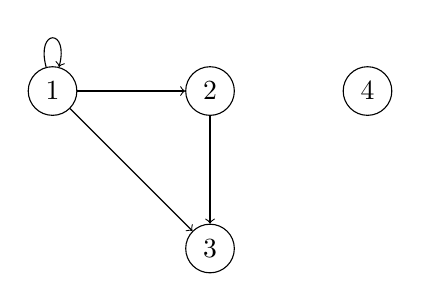
\begin{tikzpicture}[->,node distance=2cm]
  \node[draw,circle] (A) {$1$};
  \node[draw,circle] (B) [right of=A] {$2$};
  \node[draw,circle] (C) [below of=B] {$3$};
  \node[draw,circle] (D) [right of=B] {$4$};
  \draw (A) to [loop above]  (A);
  \draw (A) to  (B);
  \draw (A) to  (C);
  \draw (B) to  (C);
  \end{tikzpicture}
\intertext{આ આલેખ $\tuple{V', E}$થી જુદો છે,
  જેમાં $V' = \{1, 2, 3\}$ છે અને જે આવો દેખાય છે:}
& 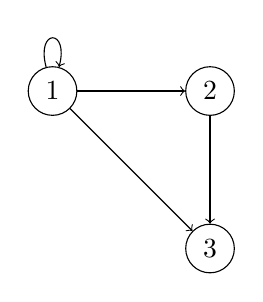
\begin{tikzpicture}[->,node distance=2cm]
  \node[draw,circle] (A) {$1$};
  \node[draw,circle] (B) [right of=A] {$2$};
  \node[draw,circle] (C) [below of=B] {$3$};
  \draw (A) to [loop above]  (A);
  \draw (A) to  (B);
  \draw (A) to  (C);
  \draw (B) to  (C);
  \end{tikzpicture}
\end{align*}
\end{ex}

\begin{prob}
  ગણ $\{1, 2, 3, 4\}$ પરના કરતાં-નાનું-અથવા-સમાન
  સંબંધ $\le$ને આલેખ તરીકે લો અને તેને અનુરૂપ આકૃતિ દોરો.
\end{prob}

\end{document}
\end{filecontents*}

% content/sets-functions-relations/relations/operations.tex
\begin{filecontents*}[overwrite]{slc-module-130.tex}
% Part: sets-functions-relations
% Chapter: relations
% Section: operations

\documentclass[../../../include/open-logic-section]{subfiles}

\begin{document}

\olfileid[gu]{sfr}{rel}{ops}
\olsection{સંબંધો પરની ક્રિયાઓ}

સંબંધોમાં ફેરફાર કરવો અથવા તેમને ભેગા કરવા ઘણી વાર ઉપયોગી
બને છે. \olref[sfr][rel][ord]{prop:stricttopartial}માં આપણે
સંબંધોના \emph{યોગગણ}નો વિચાર કર્યો હતો, જે બે સંબંધોને
જોડના ગણ તરીકે લઈએ ત્યારે તેમનો યોગગણ જ છે.
એ જ રીતે, \olref[sfr][rel][ord]{prop:partialtostrict}માં
આપણે સંબંધોના સાપેક્ષ તફાવતનો વિચાર કર્યો હતો.
અહીં સંબંધો પર કરી શકાય તેવી કેટલીક બીજી ક્રિયાઓ આપેલી છે.

\begin{defn}\ollabel{relationoperations}
ધારો કે $R$, $S$ સંબંધો છે, અને $A$ કોઈ પણ ગણ છે.

$R$નો \emph{વ્યસ્ત} એ
$R^{-1} = \Setabs{\tuple{y, x}}{\tuple{x, y} \in R}$ છે.

$R$ અને $S$નો \emph{સાપેક્ષ ગુણાકાર} એ
$(R \mid S) = \{\tuple{x, z} : \exists y(Rxy \land Syz)\}$ છે.

$R$નું $A$ પર \emph{મર્યાદન} એ
$\funrestrictionto{R}{A}= R \cap A^2$ છે.

$R$ને $A$ પર \emph{લાગુ પાડતાં મળતો ગણ} એ
$\funimage{R}{A} = \{y : (\exists x \in A)Rxy\}$ છે.
\end{defn}

\begin{ex}
ધારો કે $S \subseteq \Int^2$ એ $\Int$ પરનો અનુગામી સંબંધ છે,
એટલે કે $S = \Setabs{\tuple{x, y} \in \Int^2}{x + 1 = y}$,
જેથી $Sxy$ તો અને તો જ $x + 1 = y$.

$S^{-1}$ એ $\Int$ પરનો પુરોગામી સંબંધ છે,
એટલે કે $\Setabs{\tuple{x,y}\in\Int^2}{x -1 =y}$.

$S\mid S$ એ
$ \Setabs{\tuple{x,y}\in\Int^2}{x + 2 =y}$ છે.

$\funrestrictionto{S}{\Nat}$ એ $\Nat$ પરનો અનુગામી સંબંધ છે.

$\funimage{S}{\{1,2,3\}}$ એ $\{2, 3, 4\}$ છે.
\end{ex}

\begin{defn}[પરંપરિત સંવરણ]ધારો કે $R \subseteq A^2$ દ્વિઘટકી સંબંધ છે.

$R$નું \emph{પરંપરિત સંવરણ} એ
$R^+ = \bigcup_{0 < n \in \Nat} R^n$ છે,
જ્યાં આપણે પુનરાવર્તી રીતે $R^1 = R$ અને
$R^{n+1} = R^n \mid R$ વ્યાખ્યાયિત કરીએ છીએ.

$R$નું \emph{સ્વવાચક પરંપરિત સંવરણ} એ
$R^* = R^+ \cup \Id{A}$ છે.
\end{defn}

\begin{ex}
અનુગામી સંબંધ $S \subseteq \Int^2$ લો.
$S^2xy$ તો અને તો જ $x + 2 = y$,
$S^3xy$ તો અને તો જ $x + 3 = y$, વગેરે.
તેથી $S^+xy$ તો અને તો જ કોઈક $n \geq 1$ માટે
$x + n = y$. બીજા શબ્દોમાં, $S^+xy$ તો અને તો જ $x < y$,
અને $S^*xy$ તો અને તો જ $x \le y$.
\end{ex}

\begin{prob}
$R$નું પરંપરિત સંવરણ ખરેખર પરંપરિત છે તે દર્શાવો.
\end{prob}

\end{document}
\end{filecontents*}

% content/sets-functions-relations/relations/orders.tex
\begin{filecontents*}[overwrite]{slc-module-131.tex}
% Part: sets-functions-relations
% Chapter: relations
% Section: orders

\documentclass[../../../include/open-logic-section]{subfiles}

\begin{document}

\olfileid[gu]{sfr}{rel}{ord}
\olsection{ક્રમો}

\begin{explain}
આપણી ઘણી સરખામણીઓમાં કેટલીક વસ્તુઓને, કોઈ ચોક્કસ બાબતમાં,
બીજી વસ્તુઓ “કરતાં નાની”, “સમાન” અથવા “કરતાં મોટી”
તરીકે વર્ણવવામાં આવે છે. તેમાં \emph{ક્રમ} સંબંધો આવે છે.
પણ ક્રમ સંબંધો જુદા જુદા પ્રકારના હોય છે. દાખલા તરીકે,
કેટલાકમાં કોઈ પણ બે વસ્તુઓ તુલનીય હોવી જરૂરી છે,
બીજામાં એવું નથી. કેટલાકમાં તાદાત્મ્યનો સમાવેશ થાય છે
(જેમ કે $\le$) અને કેટલાકમાં તે બાકાત રહે છે (જેમ કે $<$).
અહીં એક વર્ગીકરણ આપણને મદદ કરશે.
\end{explain}

\begin{defn}[પૂર્વક્રમ]
સ્વવાચક અને પરંપરિત બંને હોય તેવા સંબંધને \emph{પૂર્વક્રમ} કહે છે.
\end{defn}

\begin{defn}[આંશિક ક્રમ]
વિસંમિત પણ હોય તેવા પૂર્વક્રમને \emph{આંશિક ક્રમ} કહે છે.
\end{defn}

\begin{defn}[રેખીય ક્રમ]\ollabel{def:linearorder}
તુલનાયુક્ત પણ હોય તેવા આંશિક ક્રમને \emph{સંપૂર્ણ ક્રમ}
અથવા \emph{રેખીય ક્રમ} કહે છે.
\end{defn}

\begin{ex}
દરેક રેખીય ક્રમ આંશિક ક્રમ પણ છે, અને દરેક આંશિક ક્રમ
પૂર્વક્રમ પણ છે, પણ ઊલટાં વિધાનો સાચાં નથી.
$A$ પરનો સાર્વત્રિક સંબંધ પૂર્વક્રમ છે, કારણ કે તે સ્વવાચક
અને પરંપરિત છે. પણ, જો $A$માં એક કરતાં વધુ !!{element}
હોય, તો સાર્વત્રિક સંબંધ વિસંમિત નથી, અને તેથી આંશિક ક્રમ નથી.
\end{ex}

\begin{ex}
$\Bin^*$ પરનો \emph{કરતાં વધુ લાંબું નહીં} એવો સંબંધ
$\preccurlyeq$ લો: $x \preccurlyeq y$ તો અને તો જ
$\len{x} \le \len{y}$. આ પૂર્વક્રમ છે (સ્વવાચક અને પરંપરિત),
અને તુલનાયુક્ત પણ છે, પરંતુ આંશિક ક્રમ નથી,
કારણ કે તે વિસંમિત નથી. દાખલા તરીકે,
$01 \preccurlyeq 10$ અને $10 \preccurlyeq 01$,
પણ $01 \neq 10$.
\end{ex}

\begin{ex}
ગણોના ગણ પરનો સંબંધ $\subseteq$ એક મહત્વનો આંશિક ક્રમ છે.
સામાન્ય રીતે તે રેખીય ક્રમ નથી, કારણ કે જો $a \neq b$ હોય
અને આપણે $\Pow{\{a, b\}} = \{\emptyset, \{a\}, \{b\}, \{a,b\}\}$
લઈએ, તો જોવા મળે છે કે $\{a\} \nsubseteq \{b\}$ અને
$\{a\} \neq \{b\}$ અને $\{b\} \nsubseteq \{a\}$.
\end{ex}

\begin{ex}
\emph{નિઃશેષ વિભાજ્યતા}નો સંબંધ આપણને એવો આંશિક ક્રમ આપે છે
જે રેખીય ક્રમ નથી. પૂર્ણાંકો $n$ અને $m$ માટે આપણે $n \mid m$
લખીએ, જેનો અર્થ છે કે $n$ એ $m$ને (નિઃશેષ) ભાગે છે,
એટલે કે, જો અને ફક્ત જો કોઈક પૂર્ણાંક $k$ એવો હોય કે
$m = kn$. $\Nat$ પર આ આંશિક ક્રમ છે, પણ રેખીય ક્રમ નથી:
દાખલા તરીકે, $2 \nmid 3$ અને $3 \nmid 2$ પણ.
$\Int$ પરના સંબંધ તરીકે લઈએ તો વિભાજ્યતા માત્ર પૂર્વક્રમ છે,
કારણ કે તે વિસંમિત નથી: $1 \mid -1$ અને $-1 \mid 1$
પણ $1 \neq -1$.
\end{ex}

\begin{ex}
અનુક્રમોના ગણ $A^*$ પરનો \emph{વિસ્તરણ} સંબંધ આ છે:
$s \sqsubseteq s'$ તો અને તો જ $s = \emptyseq$ (ખાલી અનુક્રમ),
$s = s'$, અથવા $s = \tuple{s_1, \dots, s_n}$ અને
$s' = \tuple{s_1, \dots, s_n, s_{n+1}, \dots, s_m}$.
જો $s \sqsubseteq s'$, તો આપણે $s$ને $s'$નો
\emph{આરંભિક ખંડ} પણ કહીએ છીએ.
$A^*$ પરનો વિસ્તરણ સંબંધ આંશિક ક્રમ છે. $A$માં બે જુદા
ઘટકો $a$ અને $b$ હોય, તો તે રેખીય ક્રમ નથી:
$ab \not\sqsubseteq ba$ અને $ba \not\sqsubseteq ab$.
\sourcecorrection{OLREA-219}{મૂળના રેખીય ન હોવાના દાવાને તેના પછીના દાખલાની બે જુદા અક્ષરો હોવાની શરત જરૂરી છે. ખાલી અથવા એક-અક્ષરી મૂળાક્ષરસમૂહ માટે બધા સાંત શબ્દો આરંભિક ખંડ દ્વારા તુલનીય છે. તેથી સામાન્ય આંશિક-ક્રમના દાવાથી રેખીય ન હોવાના શરતી દાવાને અલગ કર્યો છે.}
\end{ex}

\begin{defn}[કડક ક્રમ]
\emph{કડક ક્રમ} એવો સંબંધ છે જે અસ્વવાચક, અસંમિત અને પરંપરિત હોય.
\end{defn}

\begin{defn}[કડક રેખીય ક્રમ]\ollabel{def:strictlinearorder}
તુલનાયુક્ત પણ હોય તેવા કડક ક્રમને \emph{કડક સંપૂર્ણ ક્રમ}
અથવા \emph{કડક રેખીય ક્રમ} કહે છે.
\end{defn}

\begin{ex}
$\le$ એ કડક રેખીય ક્રમ $<$ને અનુરૂપ રેખીય ક્રમ છે.
$\subseteq$ એ કડક ક્રમ $\subsetneq$ને અનુરૂપ આંશિક ક્રમ છે.
\end{ex}

$A$ પરના કોઈ પણ કડક ક્રમ $R$માં વિકર્ણ $\Id{A}$,
એટલે કે બધા જોડ $\tuple{x, x}$, ઉમેરીને તેને આંશિક ક્રમમાં
ફેરવી શકાય છે. (આને $R$નું \emph{સ્વવાચક સંવરણ} કહે છે.)
ઊલટું, આંશિક ક્રમમાંથી $\Id{A}$ દૂર કરીને કડક ક્રમ મેળવી શકાય છે.
હવે પછીનાં બે પરિણામો આ વાત ચોક્કસ કરે છે.

\begin{prop}\ollabel{prop:stricttopartial}
જો $R$ એ $A$ પરનો કડક ક્રમ હોય, તો $R^+ = R \cup \Id{A}$
આંશિક ક્રમ છે. વધુમાં, જો $R$ કડક રેખીય ક્રમ હોય, તો
$R^+$ રેખીય ક્રમ છે.
\end{prop}

\begin{proof}
ધારો કે $R$ કડક ક્રમ છે, એટલે કે $R \subseteq A^2$ અને
$R$ અસ્વવાચક, અસંમિત અને પરંપરિત છે.
$R^+ = R \cup \Id{A}$ લો. આપણે દર્શાવવું છે કે
$R^+$ સ્વવાચક, વિસંમિત અને પરંપરિત છે.

$R^+$ દેખીતી રીતે સ્વવાચક છે, કારણ કે દરેક $x \in A$
માટે $\tuple{x, x} \in \Id{A} \subseteq R^+$.

$R^+$ વિસંમિત છે તે દર્શાવવા, પરસ્પરવિરોધ મેળવવા માટે ધારો કે
$R^+xy$ અને $R^+yx$ પણ $x \neq y$.
$\tuple{x,y} \in R \cup \Id{A}$, પણ
$\tuple{x, y} \notin \Id{A}$ હોવાથી,
$\tuple{x, y} \in R$ હોવું જોઈએ, એટલે કે $Rxy$.
એ જ રીતે, $Ryx$. પણ આ $R$ અસંમિત છે એવી ધારણાનો વિરોધ કરે છે.

પરંપરિતતા સ્થાપવા માટે ધારો કે $R^+xy$ અને $R^+yz$.
જો $\tuple{x, y} \in R$ અને $\tuple{y,z} \in R$ બંને,
તો $R$ પરંપરિત હોવાથી $\tuple{x, z} \in R$.
નહિતર, કાં $\tuple{x, y} \in \Id{A}$, એટલે કે $x = y$,
અથવા $\tuple{y, z} \in \Id{A}$, એટલે કે $y = z$.
પ્રથમ કિસ્સામાં, ધારણા પ્રમાણે $R^+yz$ અને $x = y$,
તેથી $R^+xz$. બીજા કિસ્સામાં પણ એ જ રીતે.
બંને કિસ્સામાં $R^+xz$, તેથી $R^+$ પરંપરિત પણ છે.

“વધુમાં” વાક્યાંશ અંગે, ધારો કે $R$ તુલનાયુક્ત પણ છે.
તેથી દરેક $x \neq y$ માટે, કાં $Rxy$ અથવા $Ryx$,
એટલે કે, કાં $\tuple{x, y} \in R$ અથવા $\tuple{y, x} \in R$.
$R \subseteq R^+$ હોવાથી, $R^+$ માટે પણ આ સાચું રહે છે,
તેથી $R^+$ તુલનાયુક્ત પણ છે.
\end{proof}

\begin{prop}\ollabel{prop:partialtostrict}
જો $R$ એ $A$ પરનો આંશિક ક્રમ હોય, તો
$R^- = R \setminus \Id{A}$ કડક ક્રમ છે.
વધુમાં, જો $R$ રેખીય ક્રમ હોય, તો $R^-$ કડક રેખીય ક્રમ છે.
\end{prop}

\begin{proof}
આ સ્વાધ્યાય તરીકે છોડ્યું છે.
\end{proof}

\begin{prob}
\olref[sfr][rel][ord]{prop:partialtostrict}ની સાબિતી આપો.
\end{prob}

નીચેનું સરળ પરિણામ સ્થાપે છે કે કડક રેખીય ક્રમો,
ઘટકો દ્વારા નિર્ધારિત સમાનતાને મળતો આવતો ગુણધર્મ સંતોષે છે:

\begin{prop}\ollabel{prop:extensionality-strictlinearorders}
જો $<$ એ $A$ પરનો કડક રેખીય ક્રમ હોય, તો:
\[
  (\forall a, b \in A)((\forall x \in A)(x < a \liff x < b) \lif a = b).
\]
\end{prop}

\begin{proof}
ધારો કે $(\forall x \in A)(x < a \liff x < b)$.
જો $a < b$, તો $a < a$, જે $<$ અસ્વવાચક છે એ હકીકતનો
વિરોધ કરે છે; તેથી $a \nless b$. બરાબર એ જ રીતે,
$b \nless a$. તેથી $a = b$, કારણ કે $<$ તુલનાયુક્ત છે.
\end{proof}

\end{document}
\end{filecontents*}

% content/sets-functions-relations/relations/relations-as-sets.tex
\begin{filecontents*}[overwrite]{slc-module-132.tex}
% Part: sets-functions-relations
% Chapter: relations
% Section: relations-as-sets

\documentclass[../../../include/open-logic-section]{subfiles}

\begin{document}

\olfileid[gu]{sfr}{rel}{set}
\olsection{ગણ તરીકે સંબંધો}

\begin{explain}
\olref[sfr][set][imp]{sec}માં આપણે કેટલાક મહત્વના ગણોનો ઉલ્લેખ કર્યો હતો:
$\Nat$, $\Int$, $\Rat$, $\Real$. આમાંના કેટલાક ગણોના !!{element}s
વચ્ચેના કેટલાક રસપ્રદ સંબંધો તમને ચોક્કસ યાદ હશે. દાખલા તરીકે,
આ દરેક ગણ પર એક સર્વસ્વીકૃત \emph{ક્રમ સંબંધ} છે.
\emph{તેની સાથે તાદાત્મ્ય ધરાવે છે} એવો સંબંધ પણ છે, જે દરેક વસ્તુ
પોતાની સાથે ધરાવે છે અને બીજી કોઈ વસ્તુ સાથે ધરાવતી નથી.
આગળ આપણે બીજા ઘણા રસપ્રદ સંબંધો જોઈશું, અને સંભવિત સંબંધો તો
એથીયે વધુ છે. જોકે, તેમની સમીક્ષા કરતાં પહેલાં આપણે એ નોંધથી
શરૂ કરીશું કે સંબંધોને ખાસ પ્રકારના ગણ તરીકે જોઈ શકાય છે.

આ માટે \olref[sfr][set][pai]{sec}માંથી બે બાબતો યાદ કરો. પ્રથમ,
\emph{ક્રમયુક્ત જોડ}નો ખ્યાલ યાદ કરો: $a$ અને $b$ આપેલાં હોય તો
આપણે $\tuple{a, b}$ રચી શકીએ છીએ. અહીં ઘટકોનો ક્રમ
\emph{મહત્વનો છે}. તેથી જો $a \neq b$, તો
$\tuple{a, b} \neq \tuple{b, a}$.
(આની સરખામણી અક્રમયુક્ત જોડ, એટલે કે $2$-ઘટકવાળા ગણ સાથે કરો,
જેમાં $\{a, b\}=\{b, a\}$.) બીજું, \emph{કાર્તેઝીય ગુણાકાર}નો
ખ્યાલ યાદ કરો: જો $A$ અને $B$ ગણો હોય, તો આપણે $A \times B$
રચી શકીએ છીએ; તે એવા બધા જોડ $\tuple{x, y}$નો ગણ છે જેમાં
$x \in A$ અને $y \in B$. ખાસ કરીને, $A^{2}= A \times A$
એ $A$માંથી મળતા બધા ક્રમયુક્ત જોડનો ગણ છે.

હવે આપણે એક ગણ પરનો ચોક્કસ સંબંધ લઈશું: પ્રાકૃતિક સંખ્યાઓના
ગણ $\Nat$ પરનો $<$-સંબંધ. સંખ્યાઓના એવા બધા જોડ
$\tuple{n, m}$નો ગણ લો જેમાં $n<m$, એટલે કે,
\[
  R=\Setabs{\tuple{n, m}}{n, m \in \Nat \text{ અને } n<m}.
\]
$n$ એ $m$ કરતાં નાનું હોવું અને જોડ $\tuple{n, m}$ એ
$R$નો સભ્ય હોવું, એ બે વચ્ચે ગાઢ જોડાણ છે, એટલે કે:
\[
      n<m\text{ તો અને તો જ }\tuple{n, m} \in R.
\]
ખરેખર, કોઈ માહિતી ગુમાવ્યા વિના, આપણે ગણ $R$ને
$\Nat$ પરનો $<$-સંબંધ \emph{જ છે} એમ ગણી શકીએ છીએ.

એ જ રીતે સંખ્યાઓ વચ્ચેના કોઈ પણ સંબંધ માટે આપણે $\Nat^{2}$નો
એક ઉપગણ રચી શકીએ છીએ. ઊલટું, સંખ્યાઓના જોડનો કોઈ પણ ગણ
$S \subseteq \Nat^{2}$ આપેલો હોય, તો તેને અનુરૂપ સંખ્યાઓ
વચ્ચે એક સંબંધ મળે છે, એટલે કે એવો સંબંધ જે $n$ એ $m$ સાથે
ધરાવે તો અને તો જ $\tuple{n, m} \in S$.
આ નીચેની વ્યાખ્યાને વાજબી ઠરાવે છે:
\end{explain}

\begin{defn}[દ્વિઘટકી સંબંધ]
ગણ $A$ પરનો \emph{દ્વિઘટકી સંબંધ} એ $A^{2}$નો ઉપગણ છે.
જો $R \subseteq A^{2}$ એ $A$ પરનો દ્વિઘટકી સંબંધ હોય અને
$x, y \in A$, તો આપણે ક્યારેક $\tuple{x, y} \in R$ માટે
$Rxy$ (અથવા $xRy$) લખીએ છીએ.
\end{defn}

\begin{ex}
  \ollabel{relations}
પ્રાકૃતિક સંખ્યાઓના જોડનો ગણ $\Nat^{2}$ નીચે પ્રમાણે
દ્વિપરિમાણીય શ્રેણિકમાં સૂચવી શકાય:
\[
  \begin{array}{ccccc}
  \mathbf{\tuple{ 0,0 }} & \tuple{ 0,1 } &
    \tuple{ 0,2 } & \tuple{ 0,3 } & \ldots\\
  \tuple{ 1,0 } & \mathbf{\tuple{ 1,1 }} &
    \tuple{ 1,2 } & \tuple{ 1,3 } & \ldots\\
  \tuple{ 2,0 } & \tuple{ 2,1 } &
    \mathbf{\tuple{ 2,2 }} & \tuple{ 2,3 } & \ldots\\
  \tuple{ 3,0 } & \tuple{ 3,1 } & \tuple{ 3,2 } &
    \mathbf{\tuple{ 3,3 }} & \ldots\\
  \vdots & \vdots & \vdots & \vdots & \mathbf{\ddots}
  \end{array}
\]
અહીં આપણે વિકર્ણ ઘાટા અક્ષરે દર્શાવ્યો છે, કારણ કે વિકર્ણ પર
આવેલા જોડનો બનેલો $\Nat^2$નો ઉપગણ, એટલે કે,
\[
  \{\tuple{0,0 }, \tuple{ 1,1 }, \tuple{ 2,2 }, \dots\},
  \]
એ $\Nat$ \emph{પરનો તાદાત્મ્ય સંબંધ} છે. (તાદાત્મ્ય સંબંધ
વારંવાર વપરાય છે, તેથી કોઈ પણ ગણ $A$ માટે
$\Id{A}=\Setabs{\tuple{ x,x }}{x \in A}$ એવી વ્યાખ્યા કરીએ.)
આગળ $I=\Id{\Nat}$ લઈએ.
વિકર્ણની ઉપર આવેલા બધા જોડનો ઉપગણ, એટલે કે,
\[
  L = \{\tuple{ 0,1 },\tuple{ 0,2 },\ldots,\tuple{ 1,2 },
  \tuple{ 1,3 }, \dots, \tuple{ 2,3 }, \tuple{ 2,4 },\ldots\},
\]
એ \emph{કરતાં નાનું} એવો સંબંધ છે, એટલે કે $Lnm$ તો અને તો જ
$n<m$. વિકર્ણની નીચે આવેલા જોડનો ઉપગણ, એટલે કે,
\[
  G=\{ \tuple{ 1,0 },\tuple{ 2,0 },\tuple{
    2,1 }, \tuple{ 3,0 },\tuple{ 3,1 },\tuple{ 3,2 }, \dots\},
\]
એ \emph{કરતાં મોટું} એવો સંબંધ છે, એટલે કે $Gnm$ તો અને તો જ
$n>m$. $L$ અને $I$નો યોગગણ, જેને આપણે $K=L\cup I$ કહી શકીએ,
એ \emph{કરતાં નાનું અથવા સમાન} એવો સંબંધ છે:
$Knm$ તો અને તો જ $n \le m$. એ જ રીતે, $H=G \cup I$
એ \emph{કરતાં મોટું અથવા સમાન એવો સંબંધ} છે.
આ સંબંધો $L$, $G$, $K$ અને $H$ ખાસ પ્રકારના સંબંધો છે,
જેને \emph{ક્રમો} કહે છે. $L$ અને $G$નો એવો ગુણધર્મ છે કે
કોઈ સંખ્યા પોતાની સાથે $L$ કે $G$ ધરાવતી નથી
(એટલે કે, દરેક $n$ માટે, ન તો $Lnn$, ન તો $Gnn$).
આ ગુણધર્મવાળા સંબંધોને \emph{અસ્વવાચક} કહે છે અને,
જો તેઓ ક્રમો પણ હોય, તો તેમને \emph{કડક ક્રમો} કહે છે.
\end{ex}

\begin{explain}
ક્રમો અને તાદાત્મ્ય મહત્વના અને સ્વાભાવિક સંબંધો હોવા છતાં,
એ બાબત પર ભાર મૂકવો જોઈએ કે આપણી વ્યાખ્યા પ્રમાણે $A^{2}$નો
\emph{કોઈ પણ} ઉપગણ એ $A$ પરનો સંબંધ છે, ભલે તે ગમે તેટલો
અસ્વાભાવિક કે કૃત્રિમ લાગે. ખાસ કરીને, $\emptyset$ એ કોઈ પણ
ગણ પરનો સંબંધ છે (\emph{ખાલી સંબંધ}, જે ઘટકોનું કોઈ જોડ
ધરાવતું નથી), અને $A^{2}$ પોતે પણ $A$ પરનો સંબંધ છે
(જે દરેક જોડ ધરાવે છે), જેને \emph{સાર્વત્રિક સંબંધ} કહે છે.
પણ $E=\Setabs{\tuple{n, m}}{n>5 \text{ અથવા } m \times n \ge 34}$
જેવું કંઈક પણ સંબંધ ગણાય છે.
\end{explain}

\begin{prob}
  ગણ $\Pow{\{a, b, c\}}$ પરના સંબંધ $\subseteq$ના
  !!{element}sની યાદી આપો.
\end{prob}

\end{document}
\end{filecontents*}

% content/sets-functions-relations/relations/relations.tex
\begin{filecontents*}[overwrite]{slc-module-133.tex}
% Part: sets-functions-relations
% Chapter: relations

\documentclass[../../../include/open-logic-chapter]{subfiles}

\begin{document}

\olchapter{sfr}{rel}{સંબંધો}

\slcEmbeddedImport{slc-module-132.tex}

\slcEmbeddedImport{slc-module-134.tex}

\slcEmbeddedImport{slc-module-128.tex}

\slcEmbeddedImport{slc-module-131.tex}

\slcEmbeddedImport{slc-module-129.tex}

\slcEmbeddedImport{slc-module-135.tex}

\slcEmbeddedImport{slc-module-130.tex}

\OLEndChapterHook

\end{document}
\end{filecontents*}

% content/sets-functions-relations/relations/special-properties.tex
\begin{filecontents*}[overwrite]{slc-module-134.tex}
% Part: sets-functions-relations
% Chapter: relations
% Section: special-properties

\documentclass[../../../include/open-logic-section]{subfiles}

\begin{document}

\olfileid[gu]{sfr}{rel}{prp}
\olsection{સંબંધોના વિશેષ ગુણધર્મો}

\begin{intro}
કેટલાક પ્રકારના સંબંધો એટલા સામાન્ય છે કે તેમને વિશેષ નામ
આપવામાં આવ્યાં છે. દાખલા તરીકે, $\le$ અને $\subseteq$ બંને
પોતપોતાના પ્રદેશો પર (માનો કે $\le$ માટે $\Nat$ અને
$\subseteq$ માટે $\Pow{A}$) એકસરખી રીતે સંબંધ સ્થાપે છે.
આ સંબંધો કઈ ચોક્કસ રીતે સરખા છે અને કઈ રીતે જુદા પડે છે તે
સમજવા માટે, સંબંધોમાં હોઈ શકે એવા કેટલાક વિશેષ ગુણધર્મો મુજબ
આપણે તેમનું વર્ગીકરણ કરીએ છીએ. આ વિશેષ ગુણધર્મોમાંના કેટલાક
(અથવા તેમના સંયોજનો) ખાસ મહત્વના નીવડે છે: ક્રમો અને સામ્ય સંબંધો.
\end{intro}

\begin{defn}[સ્વવાચકતા]
સંબંધ $R \subseteq A^2$ \emph{સ્વવાચક} હોય તો અને તો જ,
દરેક $x \in A$ માટે, $Rxx$.
\end{defn}

\begin{defn}[પરંપરિતતા]
સંબંધ $R \subseteq A^2$ \emph{પરંપરિત} હોય તો અને તો જ,
જ્યારે પણ $Rxy$ અને $Ryz$, ત્યારે $Rxz$ પણ.
\end{defn}

\begin{defn}[સંમિતતા]
સંબંધ $R \subseteq A^2$ \emph{સંમિત} હોય તો અને તો જ,
જ્યારે પણ $Rxy$, ત્યારે $Ryx$ પણ.
\end{defn}

\begin{defn}[વિસંમિતતા]
સંબંધ $R \subseteq A^2$ \emph{વિસંમિત} હોય તો અને તો જ,
જ્યારે પણ $Rxy$ અને $Ryx$ બંને, ત્યારે $x=y$
(અથવા, બીજા શબ્દોમાં: જો $x\neq y$, તો
કાં $\lnot Rxy$ અથવા $\lnot Ryx$).
\end{defn}

\begin{explain}
સંમિત સંબંધમાં $Rxy$ અને $Ryx$ હંમેશાં એકસાથે સાચાં હોય છે,
અથવા બંનેમાંથી એકેય સાચું હોતું નથી. વિસંમિત સંબંધમાં
$Rxy$ અને $Ryx$ એકસાથે સાચાં હોય, તો તે માત્ર $x = y$
હોય ત્યારે જ શક્ય છે. નોંધો કે આમાં $x = y$ હોય ત્યારે
$Rxy$ અને $Ryx$ સાચાં હોવાં \emph{જોઈએ} એવી માંગ નથી;
માત્ર એ શક્યતા બાકાત રખાતી નથી. તેથી વિસંમિત સંબંધ
સ્વવાચક હોઈ શકે છે, પણ દરેક વિસંમિત સંબંધ સ્વવાચક હોય
એવું નથી. એ પણ નોંધો કે વિસંમિત હોવું અને માત્ર સંમિત
ન હોવું એ જુદી શરતો છે. ખરેખર, કોઈ સંબંધ એકસાથે સંમિત
અને વિસંમિત બંને હોઈ શકે છે (દા.ત., તાદાત્મ્ય સંબંધ એવો છે).
\end{explain}

\begin{defn}[તુલનાયુક્તતા]
સંબંધ $R \subseteq A^2$ \emph{તુલનાયુક્ત} કહેવાય જો,
દરેક $x,y\in A$ માટે, $x \neq y$ હોય તો
કાં $Rxy$ અથવા $Ryx$.
\end{defn}

\begin{prob}
એવા સંબંધોના દાખલા આપો જે (a) સ્વવાચક અને સંમિત હોય પણ
પરંપરિત ન હોય, (b) સ્વવાચક અને વિસંમિત હોય,
(c) વિસંમિત અને પરંપરિત હોય પણ સ્વવાચક ન હોય, અને
(d) સ્વવાચક, સંમિત અને પરંપરિત હોય.
સંખ્યાઓ કે ગણો પરના સંબંધો વાપરશો નહીં.
\end{prob}

\begin{defn}[અસ્વવાચકતા]
સંબંધ $R \subseteq A^2$ \emph{અસ્વવાચક} કહેવાય જો,
દરેક $x \in A$ માટે, $Rxx$ સાચું ન હોય.
\end{defn}

\begin{defn}[અસંમિતતા]
સંબંધ $R \subseteq A^2$ \emph{અસંમિત} કહેવાય જો,
કોઈ પણ જોડ $x,y\in A$ માટે $Rxy$ અને $Ryx$ બંને સાચાં ન હોય.
\end{defn}

નોંધો કે જો $A \neq \emptyset$, તો $A$ પરનો કોઈ અસ્વવાચક
સંબંધ સ્વવાચક નથી અને $A$ પરનો દરેક અસંમિત સંબંધ વિસંમિત
પણ છે. જોકે, $A$માં ઓછામાં ઓછા બે જુદા ઘટકો હોય, તો
એવા $R \subseteq A^2$ છે જે સ્વવાચક પણ નથી અને અસ્વવાચક પણ નથી.
અરિક્ત $A$ પર એવા વિસંમિત સંબંધો પણ છે જે અસંમિત નથી.
\sourcecorrection{OLREA-218}{મૂળ સ્વવાચક પણ નહીં અને અસ્વવાચક પણ નહીં એવો સંબંધ હોવાના દાવામાં પ્રદેશમાં ઓછામાં ઓછા બે ઘટકો હોવાની શરત ચૂકી જાય છે. એક જ ઘટક હોય, તો તેનો પોતાની સાથેનો જોડ કાં સંબંધમાં હોય અથવા ન હોય, તેથી આ બંને ગુણધર્મોમાંથી એક લાગુ પડે છે. આ દાવાનો જરૂરી વ્યાપ સ્પષ્ટ કર્યો છે.}

\end{document}
\end{filecontents*}

% content/sets-functions-relations/relations/trees.tex
\begin{filecontents*}[overwrite]{slc-module-135.tex}
% Part: sets-functions-relations
% Chapter: relations
% Section: trees

\documentclass[../../../include/open-logic-section]{subfiles}

\begin{document}

\olfileid[gu]{sfr}{rel}{tre}
\olsection{વૃક્ષો}

તર્કશાસ્ત્રના બધા ભાગોમાં મહત્વનો ભાગ ભજવતો આંશિક ક્રમનો
એક ખાસ પ્રકાર \emph{વૃક્ષ} છે. તર્કશાસ્ત્રના પ્રાથમિક ભાગોમાં
સાંત વૃક્ષો આવે છે: દાખલા તરીકે, !!{formula}sને વાક્યરચના
વૃક્ષમાં તેમના વિઘટન દ્વારા સમજી શકાય છે, જ્યારે ઘણી
!!{derivation} પદ્ધતિઓમાં !!{derivation}s પણ સાંત વૃક્ષોનું
રૂપ ધરાવે છે.
%
વિધાનાત્મક અને પ્રથમ ક્રમના તર્કશાસ્ત્ર માટેના પૂર્ણતા પ્રમેયોની
સાબિતીમાં જ અનંત વૃક્ષો દેખાય છે, અને ગાણિતિક તર્કશાસ્ત્રમાં
સર્વત્ર તેમનો ઉપયોગ થાય છે.

ગણસિદ્ધાંતમાં વૃક્ષનો ખ્યાલ, આલેખસિદ્ધાંતમાં વૃક્ષના ખ્યાલ સાથે
ગાઢ રીતે જોડાયેલો છે. અહીં એક (સાંત) વૃક્ષનું ચિત્ર છે:

\begin{center}
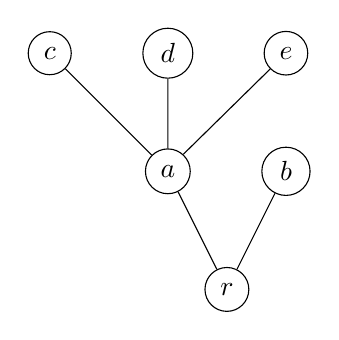
\begin{tikzpicture}[nodes={draw, circle}, -]
\node{$r$} [grow'=up]
    child { node {$a$}
        child { node {$c$} }
        child { node {$d$} }
        child { node {$e$} }
    }
    child { node {$b$} };
\end{tikzpicture}
\end{center}

સૌથી નીચેની ગાંઠ $r$ મૂળ છે. $r$ સિવાયની દરેક ગાંઠની
તરત નીચે બરાબર એક જનક ગાંઠ છે.
ગાંઠ $x$થી ધારોને અનુસરીને ઉપર જતાં ગાંઠ $y$ સુધી પહોંચી
શકાય ત્યારે $x$નો $y$ સાથેનો સંબંધ,
$x$ એ $y$નો \emph{પૂર્વજ} છે એમ સમજી શકાય.

વૃક્ષમાં પૂર્વજનો સંબંધ કડક આંશિક ક્રમ છે.
આ પરથી ગણસિદ્ધાંતની વ્યાખ્યા આપવાની પ્રેરણા મળે છે.
તે રજૂ કરવા માટે આપણને બે ખ્યાલો જોઈએ.
$\le$ વડે આંશિક ક્રમમાં ગોઠવેલા ગણ $A$માં
\emph{લઘુતમ ઘટક} એવો !!a{element} $x \in A$ છે
કે દરેક $y \in A$ માટે $x \le y$.
ગણ $\le$ વડે \emph{સુક્રમિત} હોય જો તેના દરેક
અરિક્ત ઉપગણમાં લઘુતમ ઘટક હોય.

\begin{defn}[વૃક્ષ]
\emph{વૃક્ષ} એવો જોડ $T = \tuple{A, \le}$ છે કે $A$ એક ગણ છે
અને $\le$ એ $A$ પરનો આંશિક ક્રમ છે, જેમાં એકમાત્ર લઘુતમ
ઘટક $r \in A$ છે (જેને \emph{મૂળ} કહે છે), અને
દરેક $x \in A$ માટે ગણ $\Setabs{y}{y \le x}$
એ $\le$ વડે સુક્રમિત છે.
\end{defn}

\begin{defn}[અનુગામીઓ]
ધારો કે $T = \tuple{A, \le}$ વૃક્ષ છે.
જો $x,y \in A$, $x < y$, અને $x < z < y$
થાય એવો કોઈ $z \in A$ ન હોય, તો આપણે કહીએ છીએ કે
$y$ એ $x$નો \emph{અનુગામી} છે.
\end{defn}

$x \in A$ના અનુગામીઓને તેની \emph{સંતાન ગાંઠો} પણ કહે છે.
જો $y$ એ $x$નો અનુગામી હોય, તો આપણે $x$ને $y$નો
\emph{પુરોગામી} અથવા \emph{જનક} કહીએ છીએ.

\begin{prop}
જો $\tuple{A,\le}$ વૃક્ષ હોય, તો મૂળ સિવાયના
દરેક $x \in A$નો વધુમાં વધુ એક પુરોગામી હોય.
\end{prop}

\begin{proof}
  ધારો કે $y_1 < x$ અને $y_2 < x$ અને $y_1 \neq y_2$.
  તો $\{y_1, y_2\} \subseteq \Setabs{z}{z<x}$.
  $\Setabs{z}{z<x}$ એ $\le$ વડે સુક્રમિત હોવાથી,
  તેના ઉપગણ $\{y_1, y_2\}$માં લઘુતમ ઘટક છે,
  જે દેખીતી રીતે કાં $y_1$ અથવા $y_2$ હોવો જોઈએ.
  તેથી કાં $y_1 \le y_2$ અથવા $y_2 \le y_1$.
  આપણે $y_1 \neq y_2$ ધાર્યું હતું, તેથી ખરેખર
  કાં $y_1 < y_2$ અથવા $y_2 < y_1$.
  આપણે $y_1 < x$ અને $y_2 < x$ ધાર્યું હોવાથી,
  વધુમાં કાં $y_1 < y_2 < x$ અથવા $y_2 < y_1 < x$.
  તેથી $y_1$ અને $y_2$ બંને $x$ના પુરોગામી હોઈ શકે નહીં.
\end{proof}

\begin{defn}
વૃક્ષ $T = \tuple{A, \le}$ \emph{અનંત} કહેવાય જો $A$
અનંત ગણ હોય, અને નહિતર \emph{સાંત} કહેવાય.
જો $T$માં દરેક $x \in A$ના માત્ર સાંત સંખ્યામાં અનુગામીઓ હોય,
તો આપણે કહીએ છીએ કે $T$ \emph{સાંત શાખનવાળું} છે.
\end{defn}

\begin{defn}[શાખાઓ]
વૃક્ષ $T = \tuple{A, \le}$ આપેલું હોય ત્યારે,
$T$ની \emph{શાખા} એ $T$માં સમાવેશની દૃષ્ટિએ મહત્તમ શૃંખલા છે,
એટલે કે, એવો ગણ $B \subseteq A$ કે કોઈ પણ
$x, y \in B$ માટે કાં $x \le y$ અથવા $y \le x$,
અને કોઈ પણ $z \in A \setminus B$ માટે એવો
$u \in B$ અસ્તિત્વ ધરાવે છે કે ન તો $z \le u$, ન તો $u \le z$.
%
આપણે $T$ની બધી શાખાઓના ગણને દર્શાવવા $[T]$ વાપરીએ છીએ.
\sourcecorrection{OLREA-220}{મૂળ મહત્તમ શૃંખલાની શરતમાં અપરિભાષિત ગણ $X$ વાપરે છે; વૃક્ષનો પ્રદેશ $A$ હોવાથી તેને $A$ કર્યો છે.}
\end{defn}

\begin{ex}
સાંત શાખનવાળા વૃક્ષનું એક સુપ્રસિદ્ધ ઉદાહરણ એ $0$ અને $1$ના
સાંત અનુક્રમોનું \emph{અનંત દ્વિઆધારી વૃક્ષ} છે,
જેને ક્યારેક $\{0,1\}^*$ અથવા $\Bin^*$થી દર્શાવવામાં આવે છે,
અને જે વિસ્તરણ સંબંધ $\sqsubseteq$ વડે ક્રમિત છે
(દા.ત., $101 \sqsubseteq 101101$).
કોઈ પણ દ્વિઆધારી પ્રતીકશ્રેણીને અંતે $0$ કે $1$ ઉમેરીને
હંમેશાં વિસ્તારી શકાય છે, તેથી આ વૃક્ષમાં અનંત સંખ્યામાં
ઘટકો છે: દરેક ઘટક $s$ના બરાબર બે અનુગામી $s0$ અને $s1$ છે.
તેનું મૂળ ખાલી અનુક્રમ $\emptyseq$ છે.
\end{ex}

\begin{ex}
થોડું વધુ સામાન્ય રીતે, વિસ્તરણ સંબંધ $\sqsubseteq$ સાથે
પ્રાકૃતિક સંખ્યાઓના સાંત અનુક્રમોનો ગણ $\Nat^*$ પણ વૃક્ષ છે.
તે દેખીતી રીતે સાંત શાખનવાળું નથી: દરેક $s \in \Nat^*$ના
અનંત સંખ્યામાં અનુગામી $sn$ છે, દરેક $n \in \Nat$ માટે એક.
$\sqsubseteq$ હેઠળ સંવૃત એવો દરેક અરિક્ત $A \subseteq \Nat^*$
એ $\Nat^*$નું \emph{ઉપવૃક્ષ} છે.
(એટલે કે, $A$ એવો છે કે જો $s \in A$ અને
$s' \sqsubseteq s$, તો $s' \in A$ પણ.)
બધાં સાંત વૃક્ષોને $\Nat^*$નાં સાંત ઉપવૃક્ષો તરીકે રજૂ કરી શકાય છે.
\sourcecorrection{OLREA-221}{મૂળ કોઈ પણ આરંભિક-ખંડ હેઠળ સંવૃત ઉપગણને ઉપવૃક્ષ કહે છે. ખાલી ઉપગણ પણ આ શરત સંતોષે છે, પરંતુ અહીં વૃક્ષની વ્યાખ્યામાં મૂળનું અસ્તિત્વ જરૂરી છે. તેથી આ જ વ્યાખ્યા મુજબ ઉપવૃક્ષ માટે અરિક્તતા ઉમેરેલી છે.}
\end{ex}

\begin{prop}[કેનિગનું સહાયક પ્રમેય]
જો $T = \tuple{A,\le}$ સાંત શાખનવાળું અનંત વૃક્ષ હોય,
તો $T$ને અનંત શાખા હોય છે.
\end{prop}

સંગણનીયતાના સિદ્ધાંતમાં વ્યાપકપણે વપરાતો કેનિગના સહાયક
પ્રમેયનો એક વિશેષ કિસ્સો, જેને \emph{નબળું કેનિગ સહાયક પ્રમેય}
કહે છે, આ છે: $\{0,1\}^*$ના કોઈ પણ અનંત ઉપવૃક્ષને
અનંત શાખા હોય છે.

\end{document}
\end{filecontents*}

% content/sets-functions-relations/sets-functions-relations.tex
\begin{filecontents*}[overwrite]{slc-module-136.tex}
% Part: Sets, Relations, Functions

\documentclass[../../include/open-logic-part]{subfiles}

\begin{document}

\olpart{sfr}{ગણો, સંબંધો અને ફલનો}

\begin{editorial}
  આ ફાઇલ સહજ ગણસિદ્ધાંતના ભાગના પહેલા ચાર અધ્યાયો
  મૂળની ધીમે આગળ વધતી શૈલીમાં સમાવે છે.
  સંપૂર્ણ ભાગ \verb|sets-functions-relations-complete.tex|થી સમાવાય છે.
  આ ભાગ મૂળભૂત સહજ ગણસિદ્ધાંતનો લગભગ પૂર્ણ પરિચય આપે છે.
  વિદ્યાર્થીઓને આ પૃષ્ઠભૂમિ છે એમ માની ન શકાય,
  તો અભ્યાસક્રમની શરૂઆતમાં આ સામગ્રીની સમીક્ષા કરવી યોગ્ય છે;
  ઓછામાં ઓછું ગણો, ફલનો અને સંબંધો અંગેની સામગ્રી.
  આમ બાકીના તાર્કિક વિભાગો માટે જરૂરી ગણિતીય સંકેતો વાપરવાની
  મૂળભૂત આવડત બધા વિદ્યાર્થીઓ પાસે હોવાની ખાતરી થશે.
\end{editorial}

\slcEmbeddedImport{slc-module-141.tex}

\slcEmbeddedImport{slc-module-133.tex}

\slcEmbeddedImport{slc-module-125.tex}

\slcEmbeddedImport{slc-module-153.tex}

\OLEndPartHook
\end{document}
\end{filecontents*}

% content/sets-functions-relations/sets/basics.tex
\begin{filecontents*}[overwrite]{slc-module-137.tex}
% Part: sets-functions-relations
% Chapter: sets
% Section: basics

\documentclass[../../../include/open-logic-section]{subfiles}

\begin{document}

\olfileid[gu]{sfr}{set}{bas}
\olsection{ઘટકો દ્વારા નિર્ધારિત સમાનતા}

\emph{ગણ} એટલે વસ્તુઓનો એવો સંગ્રહ, જેને {એક જ} વસ્તુ તરીકે ગણવામાં આવે.
ગણ બનાવતી વસ્તુઓને તેના \emph{ઘટકો} અથવા \emph{સભ્યો} કહે છે.
જો $x$ ગણ~$A$નો !!a{element} હોય, તો આપણે $x \in A$ લખીએ;
જો ન હોય, તો $x \notin A$ લખીએ. જે ગણમાં એક પણ !!{element} ન હોય
તેને \emph{ખાલી} ગણ કહે છે અને “$\emptyset$” વડે દર્શાવીએ છીએ.

\begin{explain}
આપણે ગણને કેવી રીતે \emph{નિર્દિષ્ટ} કરીએ છીએ, તેના !!{element}sને
કયા \emph{ક્રમમાં} મૂકીએ છીએ, કે તેના !!{element}sને \emph{કેટલી વાર}
ગણીએ છીએ, તેનાથી કોઈ ફરક પડતો નથી. તેના !!{element}s કયા છે એટલું જ
મહત્ત્વનું છે. આ વાતને આપણે નીચેના સિદ્ધાંતમાં વ્યક્ત કરીએ છીએ.
\end{explain}

\begin{defn}[ઘટકો દ્વારા નિર્ધારિત સમાનતા]
જો $A$ અને $B$ ગણો હોય, તો $A = B$ ત્યારે અને ત્યારે જ થાય જ્યારે
$A$નો દરેક !!{element} $B$નો પણ !!a{element} હોય અને ઊલટું પણ સાચું હોય.
\end{defn}

ઘટકો દ્વારા નિર્ધારિત સમાનતાનો સિદ્ધાંત કેટલીક સંજ્ઞાઓને યોગ્ય ઠરાવે છે.
સામાન્ય રીતે, આપણી પાસે $a_{1}$, \dots, $a_{n}$ વસ્તુઓ હોય, તો
$\{a_{1}, \dots, a_{n}\}$ એ \emph{ચોક્કસ એ જ} ગણ છે જેના !!{element}s
$a_1, \ldots, a_n$ છે. આપણે “\emph{ચોક્કસ એ જ}” શબ્દો પર ભાર મૂકીએ છીએ,
કારણ કે આ સિદ્ધાંત જણાવે છે કે આવો \emph{એક જ} ગણ હોઈ શકે.
હકીકતમાં, આ સિદ્ધાંત નીચેની સમાનતાઓને પણ યોગ્ય ઠરાવે છે:
  \[
    \{a, a, b\} = \{a, b\} = \{b,a\}.
  \]
આથી એ વાત સ્પષ્ટ થાય છે કે ગણોનો વિચાર કરતી વખતે તેમના !!{element}sનો
ક્રમ કે તેમને કેટલી વાર દર્શાવ્યા છે તે આપણા માટે મહત્ત્વનું નથી.

\begin{tagblock}{novice}
\begin{ex}
તમારી પાસે કેટલીક વસ્તુઓ હોય, ત્યારે તેમને એકત્ર કરીને ગણ બનાવી શકો છો.
દાખલા તરીકે, રિચર્ડનાં ભાઈબહેનોનો ગણ એક વ્યક્તિ ધરાવતો ગણ છે, અને તેને
$S=\{\textrm{રૂથ}\}$ તરીકે લખી શકાય.
$4$ કરતાં નાના ધન પૂર્ણાંકોનો ગણ $\{1, 2, 3\}$ છે, પરંતુ તેને
$\{3, 2, 1\}$ અથવા $\{1, 2, 1, 2, 3\}$ તરીકે પણ લખી શકાય.
ઘટકો દ્વારા નિર્ધારિત સમાનતાના સિદ્ધાંત અનુસાર આ બધા એક જ ગણ છે.
કારણ કે $\{1, 2, 3\}$નો દરેક !!{element} $\{3, 2, 1\}$નો
(અને $\{1, 2, 1, 2, 3\}$નો) પણ !!a{element} છે, અને ઊલટું પણ સાચું છે.
\end{ex}
\end{tagblock}

ઘણી વાર આપણે ગણના !!{element}sમાં રહેલા કોઈ સામાન્ય ગુણધર્મ દ્વારા
ગણને નિર્દિષ્ટ કરીશું. તે માટે આપણે આ સંક્ષિપ્ત સંજ્ઞા વાપરીશું:
$\Setabs{x}{\phi(x)}$. અહીં $\phi(x)$ એ એવો ગુણધર્મ દર્શાવે છે જે
ગણના !!{element}sમાં ગણાવા માટે $x$માં હોવો જરૂરી છે.

\begin{tagblock}{novice}
\begin{ex}
આપણા ઉદાહરણમાં $S$ને આ રીતે પણ નિર્દિષ્ટ કરી શક્યા હોત:
\[
S = \Setabs{x}{x \text{ રિચર્ડનાં ભાઈબહેનો પૈકી છે}}.
\]
\end{ex}
\end{tagblock}

\begin{tagblock}{math}
\begin{ex}
કોઈ સંખ્યાને \emph{પૂર્ણ સંખ્યા} ત્યારે અને ત્યારે જ કહે છે જ્યારે તે
તેના ઉચિત ભાજકોના સરવાળા જેટલી હોય (એટલે કે, તેને નિઃશેષ ભાગતા હોય
પણ તેના જેટલા ન હોય તેવા ભાજકો). દાખલા તરીકે, $6$ પૂર્ણ સંખ્યા છે,
કારણ કે તેના ઉચિત ભાજકો $1$, $2$ અને~$3$ છે, અને $6 = 1 + 2 + 3$.
હકીકતમાં, $10$ કરતાં નાના ધન પૂર્ણાંકોમાં $6$ એકમાત્ર પૂર્ણ સંખ્યા છે.
આથી, ઘટકો દ્વારા નિર્ધારિત સમાનતાનો સિદ્ધાંત વાપરીને કહી શકીએ:
\[
	\{6\} = \Setabs{x}{x\text{ પૂર્ણ સંખ્યા છે અને }0 \leq x \leq 10}
\]
જમણી બાજુની સંજ્ઞાને આપણે આ રીતે વાંચીએ: “એવા $x$નો ગણ કે $x$
પૂર્ણ સંખ્યા છે અને $0 \leq x \leq 10$”. અહીંની સમાનતા ખાતરી આપે છે
કે ગણોનો વિચાર કરતી વખતે તેમને કેવી રીતે નિર્દિષ્ટ કર્યા છે તે
મહત્ત્વનું નથી. વધુ સામાન્ય રીતે, ઘટકો દ્વારા નિર્ધારિત સમાનતાનો
સિદ્ધાંત ખાતરી આપે છે કે $\phi(x)$ ધરાવતી બધી અને માત્ર તે જ
વસ્તુઓનો ગણ અસ્તિત્વ ધરાવતો હોય, તો તે એકમાત્ર હોય.
આ અસ્તિત્વની શરત \olref[sfr][set][rus]{sec}માં સ્પષ્ટ થાય છે;
અહીં પણ તેને ધ્યાનમાં રાખીને $\Setabs{x}{\phi(x)}$ને
\emph{ચોક્કસ એ જ} ગણ કહેવું યોગ્ય છે.
\end{ex}
\end{tagblock}

ઘટકો દ્વારા નિર્ધારિત સમાનતાનો સિદ્ધાંત ગણો એક જ છે તે બતાવવાની રીત આપે છે:
$A = B$ બતાવવા માટે, જ્યારે પણ $x \in A$ હોય ત્યારે $x \in B$ પણ હોય,
અને જ્યારે પણ $y \in B$ હોય ત્યારે $y \in A$ પણ હોય, તે બતાવો.

\begin{prob}
વધુમાં વધુ એક જ ખાલી ગણ હોઈ શકે તે સાબિત કરો. એટલે કે, જો $A$ અને $B$
એવા ગણો હોય જેમાં કોઈ !!{element}s ન હોય, તો $A = B$ થાય તે બતાવો.
\end{prob}

\end{document}
\end{filecontents*}

% content/sets-functions-relations/sets/important-sets.tex
\begin{filecontents*}[overwrite]{slc-module-138.tex}
% Part: sets-functions-relations
% Chapter: sets
% Section: important-sets

\documentclass[../../../include/open-logic-section]{subfiles}

\begin{document}

\olfileid[gu]{sfr}{set}{imp}
\olsection{કેટલાક મહત્ત્વના ગણો}

\begin{ex}
આપણે મુખ્યત્વે એવા ગણોનો અભ્યાસ કરીશું જેમના !!{element}s ગાણિતિક
વસ્તુઓ હોય. આવા ચાર ગણો એટલા મહત્ત્વના છે કે તેમને ખાસ નામ આપેલાં છે:
\begin{multline*}
    \Nat = \{0, 1, 2, 3, \ldots\} \\
    \shoveright{\text{પ્રાકૃતિક સંખ્યાઓનો ગણ}}\\
    \shoveleft{\Int = \{\ldots, -2, -1, 0, 1, 2, \ldots\}} \\
    \shoveright{\text{પૂર્ણાંકોનો ગણ}}\\
    \shoveleft{\Rat = \Setabs{\nicefrac{m}{n}}{m, n \in \Int\text{ અને }n \neq 0}}\\
    \shoveright{\text{સંમેય સંખ્યાઓનો ગણ}}\\
    \shoveleft{\Real = (-\infty, \infty)}\\
    \text{વાસ્તવિક સંખ્યાઓનો ગણ (સાતત્યક)}
\end{multline*}
આ બધા \emph{અનંત} ગણો છે, એટલે કે દરેકમાં અનંત સંખ્યામાં !!{element}s છે.

આ ગણોમાં આગળ વધતા જઈએ તેમ આપણી પાસે \emph{વધુ} સંખ્યાઓ ઉમેરાતી જાય છે.
હકીકતમાં, $\Nat \subseteq \Int \subseteq \Rat \subseteq \Real$ હોવું
સ્પષ્ટ થવું જોઈએ: દરેક પ્રાકૃતિક સંખ્યા પૂર્ણાંક છે; દરેક પૂર્ણાંક સંમેય
સંખ્યા છે; અને દરેક સંમેય સંખ્યા વાસ્તવિક સંખ્યા છે.
તેવી જ રીતે, $\Nat \subsetneq \Int \subsetneq \Rat$ હોવું પણ સ્પષ્ટ
થવું જોઈએ, કારણ કે $-1$ પૂર્ણાંક છે પરંતુ પ્રાકૃતિક સંખ્યા નથી,
અને $\nicefrac{1}{2}$ સંમેય છે પરંતુ પૂર્ણાંક નથી.
$\Rat \subsetneq \Real$, એટલે કે કેટલીક વાસ્તવિક સંખ્યાઓ સંમેય નથી,
તે એટલું સ્પષ્ટ નથી\oliflabeldef{sfr:arith:real:realline}{, પરંતુ
\olref[arith][real]{realline}માં આપણે આ મુદ્દા પર પાછા આવીશું}{}.

ક્યારેક આપણે ધન પૂર્ણાંકોનો ગણ $\PosInt = \{1, 2, 3, \dots\}$ અને
માત્ર પહેલી બે પ્રાકૃતિક સંખ્યાઓ ધરાવતો ગણ $\Bin = \{0, 1\}$ પણ વાપરીશું.
\end{ex}

\begin{tagblock}{compsci}
\begin{ex}[પ્રતીકશ્રેણીઓ]
બીજું રસપ્રદ ઉદાહરણ મૂળાક્ષરસમૂહ $A$ પરથી બનતી \emph{સાંત
પ્રતીકશ્રેણીઓ}નો ગણ $A^{*}$ છે: $A$ના ઘટકોનો કોઈ પણ સાંત અનુક્રમ
$A$ પરની પ્રતીકશ્રેણી છે. દરેક મૂળાક્ષરસમૂહ~$A$ માટે, $A$ પરની
પ્રતીકશ્રેણીઓમાં આપણે \emph{ખાલી પ્રતીકશ્રેણી $\Lambda$}નો સમાવેશ કરીએ છીએ.
દાખલા તરીકે,
\begin{multline*}
\Bin^*
=\{\Lambda,0,1,00,01,10,11,\\
000,001,010,011,100,101,110,111,0000,\ldots\}.
\end{multline*}
જો $x=x_{1}\ldots x_{n}\in A^{*}$ એ $A$ના $n$ “અક્ષરો”થી બનેલી
પ્રતીકશ્રેણી હોય, તો આપણે કહીએ કે તેની \emph{લંબાઈ}~$n$ છે
અને $\len{x}=n$ લખીએ.
\end{ex}
\end{tagblock}

\begin{ex}[અનંત અનુક્રમો]
કોઈ પણ ગણ $A$ માટે આપણે $A$ના !!{element}sના અનંત અનુક્રમોનો ગણ~$A^\omega$
પણ વિચારી શકીએ. અનંત અનુક્રમ $a_1a_2a_3a_4\dots$ એ વસ્તુઓની એક
દિશામાં અનંત સુધી ચાલતી યાદી છે, જેમાંની દરેક વસ્તુ $A$નો !!a{element} છે.
\end{ex}

\end{document}
\end{filecontents*}

% content/sets-functions-relations/sets/pairs-and-products.tex
\begin{filecontents*}[overwrite]{slc-module-139.tex}
% Part: sets-functions-relations
% Chapter: sets
% Section: pairs-and-products

\documentclass[../../../include/open-logic-section]{subfiles}

\begin{document}

\olfileid[gu]{sfr}{set}{pai}
\olsection{જોડ, બહુજોડ અને કાર્તેઝીય ગુણાકાર}

\begin{explain}
ઘટકો દ્વારા નિર્ધારિત સમાનતાના સિદ્ધાંત પરથી મળે છે કે ગણના ઘટકોનો
કોઈ ક્રમ હોતો નથી. તેથી ક્રમ દર્શાવવા માટે આપણે \emph{ક્રમયુક્ત જોડ}
$\tuple{x, y}$ વાપરીએ છીએ. ક્રમ વગરની જોડ $\{x, y\}$માં ક્રમ
મહત્ત્વનો નથી: $\{x, y\} = \{y, x\}$. ક્રમયુક્ત જોડમાં તે મહત્ત્વનો છે:
જો $x \neq y$ હોય, તો $\tuple{x, y} \neq \tuple{y, x}$.

ગણસિદ્ધાંતમાં ક્રમયુક્ત જોડને કેવી રીતે સમજવી?
ખાસ કરીને, આપણે એ વિચાર જાળવવા માગીએ છીએ કે બે ક્રમયુક્ત જોડ
ત્યારે અને ત્યારે જ સમાન હોય જ્યારે તેમના પ્રથમ ઘટકો એક જ હોય
અને તેમના બીજા ઘટકો પણ એક જ હોય, એટલે કે:
\[
  \tuple{a, b}= \tuple{c, d}\text{ ત્યારે અને ત્યારે જ જ્યારે બંને }a = c \text{ અને }b=d.
\]
ગણસિદ્ધાંતમાં આપણે વીનર--કુરાતોવ્સ્કીની વ્યાખ્યા વડે
ક્રમયુક્ત જોડની વ્યાખ્યા આપી શકીએ.
\end{explain}

\begin{defn}[ક્રમયુક્ત જોડ]\ollabel{wienerkuratowski}
	$\tuple{a, b} = \{\{a\}, \{a, b\}\}$.
\end{defn}

\begin{prob}
\olref[sfr][set][pai]{wienerkuratowski} વાપરીને સાબિત કરો કે
$\tuple{a, b}= \tuple{c, d}$ ત્યારે અને ત્યારે જ થાય
જ્યારે $a = c$ અને $b=d$ બંને હોય.
\end{prob}

\begin{explain}
ક્રમયુક્ત જોડની વ્યાખ્યા નક્કી કર્યા પછી, તેને વાપરીને વધુ ગણોની
વ્યાખ્યા આપી શકીએ. દાખલા તરીકે, ક્યારેક આપણે બે કરતાં વધુ વસ્તુઓના
ક્રમયુક્ત અનુક્રમો પણ માગીએ, જેમ કે \emph{ત્રિજોડ} $\tuple{x, y, z}$,
\emph{ચતુર્જોડ} $\tuple{x, y, z, u}$, વગેરે.
ત્રિજોડને એવી ખાસ ક્રમયુક્ત જોડ તરીકે સમજી શકીએ જેનો પ્રથમ ઘટક
પોતે જ ક્રમયુક્ત જોડ હોય: $\tuple{x, y, z}$ એટલે $\tuple{\tuple{x, y},z}$.
ચતુર્જોડ માટે પણ આ જ વાત સાચી છે: $\tuple{x,y,z,u}$ એટલે
$\tuple{\tuple{\tuple{x,y},z},u}$, વગેરે.
સામાન્ય રીતે આપણે \emph{ક્રમયુક્ત $n$-જોડ} $\tuple{x_1, \dots, x_n}$ની વાત કરીએ છીએ.

ક્રમયુક્ત જોડના, અથવા અન્ય ક્રમયુક્ત $n$-જોડના, કેટલાક ગણો ઉપયોગી થશે.
\end{explain}

\begin{defn}[કાર્તેઝીય ગુણાકાર]
આપેલા ગણો $A$ અને $B$ના \emph{કાર્તેઝીય ગુણાકાર} $A \times B$ની
વ્યાખ્યા આ પ્રમાણે છે:
\[
  A \times B = \Setabs{\tuple{x, y}}{x \in A \text{ અને } y \in B}.
\]
\end{defn}

\begin{ex}
જો $A = \{0, 1\}$ અને $B = \{1, a, b\}$ હોય, તો તેમનો ગુણાકાર આ છે:
\[
A \times B = \{ \tuple{0, 1}, \tuple{0, a}, \tuple{0, b},
    \tuple{1, 1}, \tuple{1, a}, \tuple{1, b} \}.
\]
\end{ex}

\begin{ex}
જો $A$ ગણ હોય, તો $A$નો પોતાની સાથેનો ગુણાકાર $A \times A$,
$A^2$ તરીકે પણ લખાય છે. તે એવી \emph{બધી} જોડ $\tuple{x, y}$નો ગણ છે
જેમાં $x, y \in A$ હોય. આવી બધી ત્રિજોડ $\tuple{x, y, z}$નો ગણ
$A^3$ છે, વગેરે. આપણે પુનરાવર્તી વ્યાખ્યા આપી શકીએ:
\begin{align*}
  A^1 & = A\\
  A^{k+1} & = A^k \times A
\end{align*}
\end{ex}

\begin{prob}
$\{1, 2, 3\}^3$ના બધા !!{element}sની યાદી બનાવો.
\end{prob}

\begin{prop}\ollabel{cardnmprod}
જો $A$માં $n$ !!{element}s અને $B$માં $m$ !!{element}s હોય,
તો $A \times B$માં $n\cdot m$ ઘટકો હોય.
\end{prop}

\begin{proof}
$A$ના દરેક !!{element}~$x$ માટે $\tuple{x, y} \in A \times B$
સ્વરૂપના $m$ !!{element}s હોય છે.
$B_x = \Setabs{\tuple{x, y}}{y \in B}$ લો.
જ્યારે પણ $x_1 \neq x_2$ હોય ત્યારે $\tuple{x_1, y} \neq \tuple{x_2, y}$
હોવાથી $B_{x_1} \cap B_{x_2} = \emptyset$ થાય.
પરંતુ જો $A = \{x_1, \dots, x_n\}$ હોય, તો
$A \times B = B_{x_1} \cup \dots \cup B_{x_n}$,
અને તેથી તેમાં $n\cdot m$ !!{element}s હોય.

આ વાત ચિત્રરૂપે જોવા માટે $A \times B$ના !!{element}sને જાળીમાં ગોઠવો:
\[
\begin{array}{rcccc}
  B_{x_1} = & \{\tuple{x_1, y_1} & \tuple{x_1, y_2} & \dots & \tuple{x_1, y_m}\}\\
  B_{x_2} = & \{\tuple{x_2, y_1} & \tuple{x_2, y_2} & \dots & \tuple{x_2, y_m}\}\\
  \vdots & & \vdots\\
  B_{x_n} = & \{\tuple{x_n, y_1} & \tuple{x_n, y_2} & \dots & \tuple{x_n, y_m}\}
\end{array}
\]
બધા $x_i$ જુદા છે અને બધા $y_j$ પણ જુદા છે, તેથી આ જાળીની કોઈ બે જોડ
એકસરખી નથી, અને તેમાં કુલ $n\cdot m$ જોડ છે.
\end{proof}

\begin{prob}
$k$ પર ગાણિતિક આગમન વાપરીને બતાવો કે દરેક $k \ge 1$ માટે,
જો $A$માં $n$ !!{element}s હોય, તો $A^k$માં $n^k$ !!{element}s હોય.
\end{prob}

\begin{ex}
જો $A$ ગણ હોય, તો $A$ પરનો \emph{શબ્દ} એટલે $A$ના !!{element}sનો
કોઈ પણ સાંત અનુક્રમ. અનુક્રમને $A$ના !!{element}sની $n$-જોડ તરીકે સમજી શકાય.
દાખલા તરીકે, જો $A = \{a, b, c\}$ હોય, તો “$bac$” અનુક્રમને
ત્રિજોડ~$\tuple{b, a, c}$ તરીકે સમજી શકાય.
શબ્દો, એટલે કે પ્રતીકોના અનુક્રમો, સંગણકવિજ્ઞાનમાં અત્યંત મહત્ત્વના છે.
દરેક અનુક્રમને તેની લંબાઈ સાથે રાખીએ: લંબાઈ $n\ge1$નું
અનુક્રમ-ચિહ્ન $u\in A^n$ હોય, તો તેનો કોડ $\tuple{n,u}$ છે.
ખાલી અનુક્રમનો કોડ $\tuple{0,\emptyset}$ છે.
આથી $A$ પરના \emph{બધા} સાંત શબ્દોનો ગણ આ છે:
\[
A^* = \{\tuple{0,\emptyset}\}
\cup \bigcup_{n\ge1}\Setabs{\tuple{n,u}}{u\in A^n}.
\]
લંબાઈ પ્રથમ ઘટકમાં હોવાથી જુદી લંબાઈના શબ્દો ભળતા નથી.
સામાન્ય લખાણમાં આ કોડને $a$, $bac$ અથવા ખાલી શબ્દના
ચિહ્નથી જ દર્શાવીએ છીએ; અગાઉની નિશ્ચિત લંબાઈની ઘાતો બદલાતી નથી.
\sourcecorrection{OLREA-217}{મૂળ લંબાઈઓને જુદી પાડ્યા વિના ખાલી અનુક્રમ, મૂળાક્ષરસમૂહ અને તેની ઘાતોનો સામાન્ય સંઘ લખે છે. આને શબ્દોનો અનૌપચારિક સંઘ માનવો જોઈએ. કોઈ પણ ગણને મૂળાક્ષરસમૂહ માનીએ ત્યારે આ સંઘને અક્ષરશઃ લેતાં લંબાઈ ગુમાવી શકાય: $\emptyset\in A$ હોય, તો એ જ વસ્તુ ખાલી અને એક-અક્ષરી શબ્દ બંને બને. તેથી લંબાઈ-ચિહ્નિત રજૂઆત સ્પષ્ટ કરી છે.}
\begin{editorial}
મૂળનું અનૌપચારિક લખાણ:
\[
A^* = \{\emptyset\} \cup A \cup A^2 \cup A^3 \cup \dots.
\]
આને જુદી લંબાઈઓને અલગ રાખતો સંઘ સમજીને વાંચવું.
\end{editorial}
\end{ex}

\end{document}
\end{filecontents*}

% content/sets-functions-relations/sets/russells-paradox.tex
\begin{filecontents*}[overwrite]{slc-module-140.tex}
% Part: sets-functions-relations
% Chapter: sets
% Section: russells-paradox

\documentclass[../../../include/open-logic-section]{subfiles}


\begin{document}

\olfileid[gu]{sfr}{set}{rus}
\olsection{રસેલનો વિરોધાભાસ}

ઘટકો દ્વારા નિર્ધારિત સમાનતાનો સિદ્ધાંત $\phi(x)$ હોય તેવા $x$ના
\emph{ચોક્કસ એ જ} ગણ માટે $\Setabs{x}{\phi(x)}$ સંજ્ઞાને યોગ્ય ઠરાવે છે.
પરંતુ આ સિદ્ધાંત \emph{ખરેખર} માત્ર નીચેના વિચારને યોગ્ય ઠરાવે છે:
\emph{જો} એવો ગણ હોય જેના સભ્યો બરાબર $\phi$ ગુણધર્મ ધરાવતી બધી
વસ્તુઓ જ હોય, \emph{તો} આવો એક જ ગણ હોય.
બીજી રીતે કહીએ તો, કોઈ~$\phi$ નક્કી કર્યા પછી,
$\Setabs{x}{\phi(x)}$ ગણ \emph{અસ્તિત્વ ધરાવતો હોય તો} અનન્ય છે.

પરંતુ આ શરત મહત્ત્વની છે!{} ખાસ કરીને, દરેક ગુણધર્મ વડે
\emph{ગણરચના} કરી શકાતી નથી. એટલે કે કેટલાક ગુણધર્મો ગણની વ્યાખ્યા
આપતા \emph{નથી}. જો બધા ગુણધર્મો આમ કરતા હોત, તો સીધો જ
વિરોધ ઊભો થાત. આનું સૌથી જાણીતું ઉદાહરણ રસેલનો વિરોધાભાસ છે.

ગણો બીજા ગણોના !!{element}s હોઈ શકે છે---દાખલા તરીકે,
ગણ~$A$નો ઘાતગણ ગણોથી બનેલો છે.
આથી કોઈ ગણ બીજા ગણનો !!a{element} છે કે નહીં તે પૂછવું કે તપાસવું અર્થપૂર્ણ છે.
શું કોઈ ગણ પોતાનો જ સભ્ય હોઈ શકે?
ગણના ખ્યાલમાં આને બાકાત રાખે એવું કંઈ દેખાતું નથી.
દાખલા તરીકે, જો \emph{બધા} ગણો વસ્તુઓનો સંગ્રહ બનાવતા હોય,
તો કોઈને લાગે કે તેમને એક જ ગણમાં એકત્ર કરી શકાય---બધા ગણોનો ગણ.
અને તે પોતે ગણ હોવાથી બધા ગણોના ગણનો !!a{element} હોય.

પોતે પોતાનો !!a{element} ન હોવાના, એટલે કે \emph{સ્વસભ્ય ન હોવાના},
ગુણધર્મનો વિચાર કરીએ ત્યારે રસેલનો વિરોધાભાસ ઊભો થાય છે.
ધારો કે એવા બધા ગણોનો ગણ છે જે પોતે પોતાના !!a{element} નથી.
તો શું
\[
R = \Setabs{x}{x \notin x}
\]
અસ્તિત્વ ધરાવે છે? આપણે સાબિત કરી શકીએ છીએ કે તે અસ્તિત્વ ધરાવતો નથી.

\begin{thm}[રસેલનો વિરોધાભાસ]\ollabel{thm:russells-paradox}
	$R = \Setabs{x}{x \notin x}$ એવો કોઈ ગણ નથી.
\end{thm}

\begin{proof}
જો $R = \Setabs{x}{x \notin x}$ અસ્તિત્વ ધરાવતો હોય, તો
$R \in R$ ત્યારે અને ત્યારે જ થાય જ્યારે $R \notin R$ હોય,
જે પરસ્પરવિરોધ છે.
\end{proof}

\begin{tagblock}{novice}
\begin{explain}
આ સાબિતીને વધુ ધીમેથી સમજીએ. જો $R$ અસ્તિત્વ ધરાવતો હોય, તો
$R \in R$ છે કે નહીં તે પૂછવું અર્થપૂર્ણ છે.
ધારો કે ખરેખર $R \in R$ છે. હવે $R$ની વ્યાખ્યા એવા બધા ગણોના ગણ
તરીકે આપેલી છે જે પોતે પોતાના !!{element}s નથી.
આથી, જો $R \in R$ હોય, તો $R$ પોતે $R$ને વ્યાખ્યાયિત કરતો ગુણધર્મ ધરાવતો નથી.
પરંતુ આ ગુણધર્મ ધરાવતા ગણો જ $R$માં છે, તેથી $R$ એ $R$નો
!!a{element} હોઈ શકે નહીં, એટલે કે $R \notin R$.
પરંતુ $R$ એકસાથે $R$નો !!a{element} હોય અને ન પણ હોય તે શક્ય નથી.
આથી આપણને પરસ્પરવિરોધ મળે છે.

$R \in R$ની ધારણા પરસ્પરવિરોધ તરફ દોરી જાય છે, તેથી $R \notin R$ છે.
પરંતુ આ પણ પરસ્પરવિરોધ તરફ દોરી જાય છે!{}
કારણ કે જો $R \notin R$ હોય, તો $R$ પોતે $R$ને વ્યાખ્યાયિત કરતો ગુણધર્મ
ધરાવે છે, અને તેથી, બીજા બધા સ્વસભ્ય ન હોય તેવા ગણોની જેમ,
$R$ પણ $R$નો !!a{element} હોય.
ફરીથી, તે એકસાથે $R$નો !!a{element} ન હોય અને હોય પણ ખરો તે શક્ય નથી.
\end{explain}
\end{tagblock}

\begin{digress}
રસેલના વિરોધાભાસમાં ન ફસાતો ગણસિદ્ધાંત કેવી રીતે રચી શકાય?
એટલે કે $R = \Setabs{x}{x \notin x}$ અસ્તિત્વ ધરાવે છે એવો
\emph{અસંગત} દાવો ટાળતો ગણસિદ્ધાંત કેવી રીતે રચી શકાય?
તે માટે એવી પૂર્વધારણાઓ નક્કી કરવી પડે જે ગણો ક્યારે અસ્તિત્વ ધરાવે
છે (અને ક્યારે નથી ધરાવતા) તે કહેવા માટે અત્યંત ચોક્કસ શરતો આપે.

આ પ્રકરણમાં રૂપરેખા આપેલો ગણસિદ્ધાંત આવું કરતો નથી.
તે \emph{ખરેખર સહજ ખ્યાલો પર આધારિત} છે.
તે માત્ર એટલું કહે છે કે ગણો ઘટકો દ્વારા નિર્ધારિત સમાનતાના સિદ્ધાંતને
અનુસરે છે અને જો તમારી પાસે કેટલાક ગણો હોય, તો તેમનો યોગગણ,
છેદગણ વગેરે બનાવી શકો છો.
ગણસિદ્ધાંતને આના કરતાં વધુ ચોકસાઈથી વિકસાવવો શક્ય છે.
\oliflabeldef{cumul:::part}{આ ચોકસાઈ આપણે ભાગ \olref[cumul][][]{part}
માટે રાખીશું. હાલ આપણે સહજ ખ્યાલોના આધારે આગળ વધીશું
અને કાળજીપૂર્વક વિરોધો ટાળવાનો પ્રયાસ કરીશું.}{}
\end{digress}


\end{document}
\end{filecontents*}

% content/sets-functions-relations/sets/sets.tex
\begin{filecontents*}[overwrite]{slc-module-141.tex}
% Part: sets-functions-relations
% Chapter: sets

\documentclass[../../../include/open-logic-chapter]{subfiles}

\begin{document}

\olchapter{sfr}{set}{ગણો}

\slcEmbeddedImport{slc-module-137.tex}

\slcEmbeddedImport{slc-module-142.tex}

\slcEmbeddedImport{slc-module-138.tex}

\slcEmbeddedImport{slc-module-143.tex}

\slcEmbeddedImport{slc-module-139.tex}

\slcEmbeddedImport{slc-module-140.tex}

\OLEndChapterHook

\end{document}
\end{filecontents*}

% content/sets-functions-relations/sets/subsets.tex
\begin{filecontents*}[overwrite]{slc-module-142.tex}
% Part: sets-functions-relations
% Chapter: sets
% Section: subsets

\documentclass[../../../include/open-logic-section]{subfiles}

\begin{document}

\olfileid[gu]{sfr}{set}{sub}
\olsection{ઉપગણો અને ઘાતગણો}

\begin{explain}
આપણે ઘણી વાર ગણોની તુલના કરવા માગીશું. આવી તુલનાનો એક સ્પષ્ટ પ્રકાર આ છે:
\emph{એક ગણમાં જે કંઈ છે તે બધું બીજા ગણમાં પણ છે}.
આ પરિસ્થિતિ એટલી મહત્ત્વની છે કે તેના માટે આપણે નવી સંજ્ઞા રજૂ કરીએ છીએ.
\end{explain}

\begin{defn}[ઉપગણ]
જો ગણ $A$નો દરેક !!{element} $B$નો પણ !!a{element} હોય, તો આપણે કહીએ
કે $A$ એ $B$નો \emph{ઉપગણ} છે, અને $A \subseteq B$ લખીએ.
જો $A$ એ $B$નો ઉપગણ ન હોય, તો $A \not\subseteq B$ લખીએ.
જો $A \subseteq B$ પરંતુ $A \neq B$ હોય, તો $A \subsetneq B$ લખીએ
અને કહીએ કે $A$ એ $B$નો \emph{ઉચિત ઉપગણ} છે.
\end{defn}

\begin{ex}
દરેક ગણ પોતાનો જ ઉપગણ છે, અને $\emptyset$ દરેક ગણનો ઉપગણ છે.
યુગ્મ પ્રાકૃતિક સંખ્યાઓનો ગણ પ્રાકૃતિક સંખ્યાઓના ગણનો ઉપગણ છે.
વળી, $\{ a, b \} \subseteq \{ a, b, c \}$.
પરંતુ $\{ a, b, e \}$ એ $\{ a, b, c \}$નો ઉપગણ નથી.
\end{ex}

\begin{ex}
સંખ્યા $2$ પૂર્ણાંકોના ગણનો !!{element} છે, જ્યારે યુગ્મ સંખ્યાઓનો ગણ
પૂર્ણાંકોના ગણનો ઉપગણ છે. તેમ છતાં, કોઈ ગણ બીજા ગણનો !!a{element}
અને ઉપગણ \emph{બંને} હોઈ શકે. દા.ત.,
$\{0\} \in \{0, \{0\}\}$ અને $\{0\} \subseteq \{0, \{0\}\}$ પણ છે.
\end{ex}

ઘટકો દ્વારા નિર્ધારિત સમાનતાનો સિદ્ધાંત ગણો એક જ હોવાની કસોટી આપે છે:
$A = B$ ત્યારે અને ત્યારે જ થાય જ્યારે $A$નો દરેક !!{element}
$B$નો પણ !!a{element} હોય અને ઊલટું પણ સાચું હોય.
“ઉપગણ”ની વ્યાખ્યા અનુસાર $A \subseteq B$ એ આ કસોટીના પહેલા ભાગનું જ
નિરૂપણ છે: $A$નો દરેક !!{element} $B$નો પણ !!a{element} છે.
અલબત્ત, $A$ અને $B$ની અદલાબદલી કરીએ તો પણ આ વ્યાખ્યા લાગુ પડે છે:
$B \subseteq A$ ત્યારે અને ત્યારે જ થાય જ્યારે $B$નો દરેક !!{element}
$A$નો પણ !!a{element} હોય. આ તો ઘટકો દ્વારા નિર્ધારિત સમાનતાના
સિદ્ધાંતનો “ઊલટું પણ” એવો ભાગ જ છે.
બીજા શબ્દોમાં, આ સિદ્ધાંત અનુસાર ગણો ત્યારે અને ત્યારે જ સમાન હોય
જ્યારે તેઓ એકબીજાના ઉપગણો હોય.

\begin{prop}
$A = B$ ત્યારે અને ત્યારે જ થાય જ્યારે $A \subseteq B$ અને $B \subseteq A$ બંને હોય.
\end{prop}

કેટલીક વધુ ઉપયોગી સંજ્ઞાઓ રજૂ કરવાની આ સારી તક છે.
$A$ એ $B$નો ઉપગણ ક્યારે કહેવાય તેની વ્યાખ્યા આપતી વખતે આપણે
“$A$નો દરેક !!{element} \dots” કહ્યું હતું, અને “$\dots$”ની જગ્યાએ
“$B$નો !!a{element} છે” મૂક્યું હતું.
પરંતુ આવાં વિધાનોનું આ \emph{સ્વરૂપ} એટલું સામાન્ય છે કે તેના માટે
ઔપચારિક સંજ્ઞા રજૂ કરવી ઉપયોગી થશે.

\begin{defn}\ollabel{forallxina}
$(\forall x \in A)\phi$ એ $\forall x(x \in A \lif
\phi)$નું સંક્ષિપ્ત સ્વરૂપ છે. તેવી જ રીતે, $(\exists x \in A)\phi$
એ $\exists x(x \in A \land \phi)$નું સંક્ષિપ્ત સ્વરૂપ છે.
\end{defn}

આ સંજ્ઞા વાપરીને આપણે કહી શકીએ કે $A \subseteq B$ ત્યારે અને ત્યારે જ
થાય જ્યારે $(\forall x \in A)x \in B$ હોય.

હવે આપણે એક ખાસ પ્રકારના ગણનો વિચાર કરીએ: આપેલા ગણના બધા ઉપગણોનો ગણ.

\begin{defn}[ઘાતગણ]
ગણ~$A$ના બધા ઉપગણોથી બનેલા ગણને $A$નો \emph{ઘાતગણ} કહે છે
અને $\Pow{A}$ વડે દર્શાવીએ છીએ.
  \[
    \Pow{A} = \Setabs{B}{B \subseteq A}
  \]
\end{defn}

\begin{ex}
$\{ a, b, c \}$ના બધા શક્ય ઉપગણો કયા છે? તે આ છે:
$\emptyset$, $\{a \}$, $\{b\}$, $\{c\}$, $\{a, b\}$, $\{a, c\}$, $\{b,
c\}$, $\{a, b, c\}$. આ બધા ઉપગણોનો ગણ $\Pow{\{a,b,c\}}$ છે:
\[
\Pow{\{ a, b, c \}} = \{\emptyset, \{a \}, \{b\}, \{c\}, \{a, b\},
\{b, c\}, \{a, c\}, \{a, b, c\}\}
\]
\end{ex}

\begin{prob}
$\{a, b, c, d\}$ના બધા ઉપગણોની યાદી બનાવો.
\end{prob}

\begin{prob}
જો $A$માં $n$ !!{element}s હોય, તો $\Pow{A}$માં $2^n$
!!{element}s હોય તે બતાવો.
\end{prob}

\end{document}
\end{filecontents*}

% content/sets-functions-relations/sets/unions-and-intersections.tex
\begin{filecontents*}[overwrite]{slc-module-143.tex}
% Part: sets-functions-relations
% Chapter: sets
% Section: unions-and-intersections

\documentclass[../../../include/open-logic-section]{subfiles}

\begin{document}

\olfileid[gu]{sfr}{set}{uni}
\olsection{યોગગણો અને છેદગણો}

\begin{explain}
\olref[sfr][set][bas]{sec}માં આપણે ગુણધર્મ દ્વારા ગણોની વ્યાખ્યા,
એટલે કે $\Setabs{x}{\phi(x)}$ સ્વરૂપની વ્યાખ્યાઓ રજૂ કરી હતી.
અહીં આપણે કોઈ ગુણધર્મ~$\phi$નો ઉપયોગ કરીએ છીએ, અને આ ગુણધર્મમાં
અગાઉ વ્યાખ્યાયિત કરેલા ગણોનો ઉલ્લેખ હોઈ શકે છે.
દાખલા તરીકે, જો $A$ અને~$B$ ગણો હોય, તો
$\Setabs{x}{x \in A \lor x \in B}$ એ બધી વસ્તુઓનો ગણ છે જે $A$ અથવા~$B$ના
!!{element}s હોય; એટલે કે તે $A$ અને~$B$ના !!{element}sને એકત્ર કરતો ગણ છે.
આને \olref{fig:union}માં દર્શાવ્યા મુજબ જોઈ શકાય, જ્યાં રંગેલો વિસ્તાર
બંને ગણો $A$ અને~$B$ના !!{element}sને એકસાથે દર્શાવે છે.

\begin{figure}
  \olasset{assets/diagrams/union.tikz}
  \caption{બે ગણોનો યોગગણ $A \cup B$ એ $A$ના !!{element}s અને
  $B$ના !!{element}sને એકત્ર કરતાં મળતો ગણ છે.}
  \ollabel{fig:union}
\end{figure}

ગણો પરની આ ક્રિયા---તેમને એકત્ર કરવાની ક્રિયા---ખૂબ ઉપયોગી અને સામાન્ય છે,
તેથી આપણે તેને ઔપચારિક નામ અને સંકેત આપીએ છીએ.
\end{explain}

\begin{defn}[યોગગણ]
બે ગણો $A$ અને $B$નો \emph{યોગગણ}, જેને $A \cup B$ લખીએ છીએ,
એ બધી વસ્તુઓનો ગણ છે જે $A$ના, $B$ના, અથવા બંનેના !!{element}s હોય.
\[
A \cup B = \Setabs{x}{x \in A \lor x \in B}
\]
\end{defn}

\begin{ex}
!!{element}s કેટલી વાર આવ્યા છે તે મહત્ત્વનું ન હોવાથી, કોઈ !!a{element}
સામાન્ય હોય તેવા બે ગણોના યોગગણમાં તે !!{element} એક જ વાર આવે છે.
દા.ત., $\{ a, b, c\} \cup \{ a, 0, 1\} = \{a, b, c, 0, 1\}$.

ગણ અને તેના કોઈ ઉપગણનો યોગગણ મોટો ગણ પોતે જ છે:
$\{a, b, c \} \cup \{a \} = \{a, b, c\}$.

ગણ અને ખાલી ગણનો યોગગણ તે ગણ પોતે જ છે:
$\{a, b, c \} \cup \emptyset = \{a, b, c \}$.
\end{ex}

\begin{prob}
જો $A \subseteq B$ હોય, તો $A \cup B = B$ થાય તે સાબિત કરો.
\end{prob}

\begin{explain}
આપણે યોગક્રિયાની “દ્વૈત” ક્રિયાનો પણ વિચાર કરી શકીએ.
આ ક્રિયા એવા બધા !!{element}sનો ગણ બનાવે છે જે $A$ના !!{element}s
હોય અને $B$ના પણ !!{element}s હોય.
આ ક્રિયાને \emph{છેદક્રિયા} કહે છે અને તેને \olref{fig:intersection}માં
દર્શાવ્યા પ્રમાણે ચિત્રી શકાય.
\begin{figure}
  \olasset{assets/diagrams/intersection.tikz}
  \caption{બે ગણોનો છેદગણ $A \cap B$ એ તેમના સામાન્ય !!{element}sનો ગણ છે.}
  \ollabel{fig:intersection}
\end{figure}
\end{explain}

\begin{defn}[છેદગણ]
બે ગણો $A$ અને $B$નો \emph{છેદગણ}, જેને $A \cap B$ લખીએ છીએ,
એ બધી વસ્તુઓનો ગણ છે જે $A$ અને~$B$ બંનેના !!{element}s હોય.
\[
A \cap B = \Setabs{x}{x \in A \land x \in B}
\]
જો બે ગણોનો છેદગણ ખાલી હોય, તો તેમને \emph{અલગ ગણો} કહે છે.
આનો અર્થ એ છે કે તેમનામાં એક પણ સામાન્ય !!{element} નથી.
\end{defn}

\begin{ex}
જો બે ગણોમાં એક પણ સામાન્ય !!{element} ન હોય, તો તેમનો છેદગણ ખાલી છે:
$\{ a, b, c\} \cap \{ 0, 1\} = \emptyset$.

જો બે ગણોમાં સામાન્ય !!{element}s હોય, તો તેમનો છેદગણ એ બધા
!!{element}sનો ગણ છે: $\{a, b, c \} \cap \{a, b, d \} = \{a, b\}$.

ગણ અને તેના કોઈ ઉપગણનો છેદગણ નાનો ગણ પોતે જ છે:
$\{a, b, c\} \cap \{a, b\} = \{a, b\}$.

કોઈ પણ ગણ અને ખાલી ગણનો છેદગણ ખાલી છે:
$\{a, b, c \} \cap \emptyset = \emptyset$.
\end{ex}

\begin{prob}
જો $A \subseteq B$ હોય, તો $A \cap B = A$ થાય તે ચોકસાઈપૂર્વક સાબિત કરો.
\end{prob}

\begin{explain}
આપણે બે કરતાં વધુ ગણોનો યોગગણ કે છેદગણ પણ બનાવી શકીએ.
સામાન્ય રીતે આ કરવાની એક સુઘડ રીત નીચે મુજબ છે:
ધારો કે જે બધા ગણોનો યોગગણ (અથવા છેદગણ) બનાવવો છે તેમને
આપણે એક જ ગણમાં એકત્ર કરીએ. ત્યાર પછી, આપણા બધા મૂળ ગણોના
યોગગણની વ્યાખ્યા એ બધી વસ્તુઓના ગણ તરીકે કરી શકીએ જે આ ગણના
ઓછામાં ઓછા એક !!{element}માં હોય; અને છેદગણની વ્યાખ્યા એ બધી
વસ્તુઓના ગણ તરીકે કરી શકીએ જે આ ગણના દરેક !!{element}માં હોય.
\end{explain}

\begin{defn}
જો $A$ ગણોનો ગણ હોય, તો $\bigcup A$ એ $A$ના !!{element}sના
!!{element}sનો ગણ છે:
\begin{align*}
\bigcup A & = \Setabs{x}{x \text{ ગણ } A \text{ના કોઈ !!a{element}માં છે}},
\text{ એટલે કે,}\\
& = \Setabs{x}{\text{એવો } B \in A
  \text{ છે કે } x \in B}
\end{align*}
\end{defn}

\begin{defn}
જો $A$ ગણોનો અરિક્ત ગણ હોય, તો $\bigcap A$ એ બધી વસ્તુઓનો ગણ છે જે
$A$ના બધા ઘટકોમાં સામાન્ય હોય:
\begin{align*}
\bigcap A & = \Setabs{x}{x \text{ ગણ } A \text{ના દરેક !!{element}માં છે}},
\text{ એટલે કે,}\\
 & = \Setabs{x}{\text{દરેક } B \in A, \text{ માટે } x \in B}
\end{align*}
\sourcecorrection{OLREA-216}{મૂળ છેદગણની આ વ્યાખ્યામાં ગણોના કુટુંબને અરિક્ત હોવાની શરત આપતું નથી. ખાલી કુટુંબ માટે દરેક સભ્યગણમાં હોવાની શરત આપમેળે સાચી છે, તેથી અપ્રતિબંધિત વ્યાખ્યા બધી વસ્તુઓને સમાવી લે; આ ગણ હોવાનું માની ન શકાય. તેથી અહીં અરિક્ત કુટુંબ લીધું છે. નિશ્ચિત સાર્વત્રિક ગણ $U$ના ઉપગણો માટે ખાલી છેદગણને $U$ લેવાની જુદી રૂઢિ વાપરી શકાય; ખાલી યોગગણ હંમેશાં $\emptyset$ છે.}
\end{defn}

\begin{ex}
ધારો કે $A = \{ \{ a, b \}, \{ a, d, e \}, \{ a, d \} \}$.
તો $\bigcup A = \{ a, b, d, e \}$ અને $\bigcap A = \{ a \}$.
\end{ex}
\begin{prob}
જો $A$ ગણ હોય અને $A \in B$ હોય, તો $A \subseteq \bigcup B$ થાય તે બતાવો.
\end{prob}

ગણોના અનુક્રમ $A_1$, $A_2$, \dots માટે પણ આપણે આમ જ કરી શકીએ:
\begin{align*}
\bigcup_i A_i & = \Setabs{x}{x \text{ કોઈ એક } A_i \text{માં છે}}\\
\bigcap_i A_i & = \Setabs{x}{x \text{ દરેક } A_i \text{માં છે}}.
\end{align*}

જ્યારે આપણી પાસે ગણોનો \emph{સૂચકગણ} હોય, એટલે કે એવો ગણ $I$ હોય કે
દરેક $i \in I$ માટે આપણે $A_i$નો વિચાર કરતા હોઈએ,
ત્યારે આ સંક્ષિપ્ત સંજ્ઞાઓ પણ વાપરી શકીએ:
\begin{align*}
	\bigcup_{i \in I} A_i & = \bigcup \Setabs{A_i }{i \in I}\\
	\bigcap_{i \in I} A_i & = \bigcap\Setabs{A_i}{i \in I}
\end{align*}
છેદગણ માટે અહીં $I$ અરિક્ત છે. $I$ ખાલી હોય, તો
ઉપર સમજાવેલી નિશ્ચિત સાર્વત્રિક ગણની રૂઢિ જરૂરી છે.

છેલ્લે, આપણે $A$ના એવા બધા !!{element}sના ગણનો વિચાર કરવા માગીએ
જે $B$માં નથી. તેને \olref{difference}માં દર્શાવ્યા પ્રમાણે ચિત્રી શકાય.

\begin{figure}
  \olasset{assets/diagrams/difference.tikz}
  \caption{બે ગણોનો તફાવત ગણ $A \setminus B$ એ $A$ના એવા
  !!{element}sનો ગણ છે જે $B$ના પણ !!{element}s નથી.}
  \ollabel{difference}
\end{figure}

\begin{defn}[તફાવત ગણ]
\emph{તફાવત ગણ}~$A \setminus B$ એ $A$ના એવા બધા !!{element}sનો ગણ છે
જે $B$ના પણ !!{element}s નથી, એટલે કે,
\[
A\setminus B = \Setabs{x}{x\in A \text{ અને } x \notin B}.
\]
\end{defn}

\begin{prob}
જો $A \subsetneq B$ હોય, તો $B \setminus A \neq \emptyset$ થાય તે સાબિત કરો.
\end{prob}

\end{document}
\end{filecontents*}

% content/sets-functions-relations/size-of-sets/comparing-size.tex
\begin{filecontents*}[overwrite]{slc-module-144.tex}
% Part:sets-functions-relations
% Chapter: size-of-sets
% Section: comparing-sizes

\documentclass[../../../include/open-logic-section]{subfiles}

\begin{document}

\olfileid[gu]{sfr}{siz}{car}

\olsection{જુદાં કદના ગણો અને કૅન્ટૉરનું પ્રમેય}

\begin{explain}
બે ગણોનું કદ સરખું હોવાના વિચારને આપણે ચોક્કસ રીતે રજૂ કર્યો છે.
એક ગણ બીજા કરતાં નાનો હોવાના વિચારને પણ ચોક્કસ રીતે રજૂ કરી શકાય.
“નાનો (અથવા સામ્ય ગણ)” હોવાની આપણી વ્યાખ્યામાં બંને ગણો વચ્ચેના
!!a{bijection}ને બદલે પહેલા ગણમાંથી બીજા ગણમાં જતા !!a{injection}ની
જરૂર પડશે. આવું ફલન અસ્તિત્વમાં હોય, તો પહેલા ગણનું કદ બીજા
ગણના કદ કરતાં ઓછું અથવા બરાબર છે. સહજ રીતે, એક ગણમાંથી બીજા ગણમાં
જતો !!a{injection} ખાતરી આપે છે કે ફલનના વિસ્તારમાં તેના પ્રદેશ
જેટલા તો !!{element}s છે જ, કારણ કે પ્રદેશના કોઈ બે !!{element}sનું
નિરૂપણ વિસ્તારના એક જ !!{element} પર થતું નથી.
\end{explain}

\begin{defn}
$A$ એ $B$ કરતાં \emph{મોટો નથી}, જે $\cardle{A}{B}$ લખીએ,
જો અને માત્ર જો કોઈ !!a{injection} $f \colon A \to B$ હોય.
\end{defn}

સ્પષ્ટ છે કે આ સંબંધ સ્વવાચક અને પરંપરિત છે, પરંતુ સંમિત નથી
(આ સાબિત કરવાનું અભ્યાસ તરીકે છોડ્યું છે). એક ગણ બીજા કરતાં
(ચુસ્તપણે) નાનો હોવાનું જણાવતો ખ્યાલ પણ રજૂ કરી શકાય છે.

\begin{defn}
$A$ એ $B$ કરતાં \emph{નાનો} છે, જે $\cardless{A}{B}$ લખીએ,
જો અને માત્ર જો કોઈ !!a{injection}~$f\colon A \to B$ હોય પરંતુ
કોઈ !!{bijection}~$g\colon A \to B$ ન હોય; એટલે કે,
$\cardle{A}{B}$ અને $\cardneq{A}{B}$.
\end{defn}

સ્પષ્ટ છે કે આ સંબંધ અસ્વવાચક અને પરંપરિત છે. (આ સાબિત કરવાનું
અભ્યાસ તરીકે છોડ્યું છે.) આ સંજ્ઞા વાપરીને કહી શકાય કે ગણ $A$ એ
!!{enumerable} હોય જો અને માત્ર જો $\cardle{A}{\Nat}$, અને પસંદગીની સ્વયંસિદ્ધિ માનીએ ત્યારે $A$ એ
!!{nonenumerable} હોય જો અને માત્ર જો $\cardless{\Nat}{A}$.
આથી
\oliflabeldef{sfr:siz:nen-alt:thm:nonenum-pownat}{%
\olref[sfr][siz][nen-alt]{thm:nonenum-pownat}ને
$\cardless{\Nat}{\Pow{\Nat}}$ એવા અવલોકન તરીકે}{%
\olref[sfr][siz][nen]{thm:nonenum-pownat}ને
$\cardless{\PosInt}{\Pow{\PosInt}}$ એવા અવલોકન તરીકે} ફરી રજૂ
કરી શકાય છે. હકીકતમાં, \citet{Cantor1892}એ સાબિત કર્યું કે આ છેલ્લી
વાત \emph{સર્વથા સામાન્ય} છે:

\begin{thm}[કૅન્ટૉર]\ollabel{thm:cantor}
કોઈ પણ ગણ $A$ માટે, $\cardless{A}{\Pow{A}}$.
\end{thm}

\begin{proof}
નિરૂપણ $f(x) = \{x\}$ એ !!a{injection} $f \colon A \to \Pow{A}$
છે, કારણ કે $x \neq y$ હોય, તો ઘટકો દ્વારા નિર્ધારિત સમાનતાના
સિદ્ધાંતથી $\{x\} \neq \{y\}$ પણ હોય, અને તેથી $f(x) \neq f(y)$.
આથી $\cardle{A}{\Pow{A}}$.

\begin{editorial}
\olref[nen]{sec} સમાવેલો હોય તો આપણે વિગતવાર સાબિતી રજૂ કરીએ છીએ;
અન્યથા \olref[nen-alt]{sec}ને અનુરૂપ ટૂંકી સાબિતી રજૂ કરીએ છીએ.
\end{editorial}

\oliflabeldef{sfr:siz:nen:sec}{%
  હવે આપણે બતાવીશું કે !!a{surjective} ફલન~$g\colon A \to
  \Pow{A}$ અસ્તિત્વમાં હોઈ જ ન શકે, તેથી !!a{bijective} ફલન તો
  અસ્તિત્વમાં ન જ હોય, અને આમ $\cardneq{A}{\Pow{A}}$. વિરોધાર્થે,
  ધારો કે $g\colon A \to \Pow{A}$. $g$ સર્વત્ર વ્યાખ્યાયિત હોવાથી દરેક
  $x \in A$નું નિરૂપણ કોઈ ઉપગણ $g(x) \subseteq A$ પર થાય છે.
  આપણે બતાવી શકીએ કે $g$ વ્યાપ્ત ન હોઈ શકે. તે માટે આપણે એવો
  ઉપગણ~$\overline{A} \subseteq A$ વ્યાખ્યાયિત કરીએ છીએ જે
  વ્યાખ્યા પ્રમાણે $g$ના વિસ્તારમાં હોઈ ન શકે. ધારો કે
  \[
  \overline{A} = \Setabs{x \in A}{x \notin g(x)}.
  \]
  દરેક $x \in A$ માટે $g(x)$ વ્યાખ્યાયિત હોવાથી $\overline{A}$
  સ્પષ્ટ રીતે $A$નો સુવ્યાખ્યાયિત ઉપગણ છે. પરંતુ તે $g$ના વિસ્તારમાં
  હોઈ ન શકે. મનસ્વી $x \in A$ લો; આપણે બતાવીશું કે
  $\overline{A} \neq g(x)$. જો $x \in g(x)$, તો તે
  $x \notin g(x)$ને સંતોષતો નથી, અને તેથી $\overline{A}$ની વ્યાખ્યા
  પ્રમાણે $x \notin \overline{A}$. જો $x \in \overline{A}$, તો
  તેણે $\overline{A}$નો વ્યાખ્યાયી ગુણધર્મ સંતોષવો જ પડે; એટલે કે,
  $x \in A$ અને $x \notin g(x)$. $x$ મનસ્વી હોવાથી, આ બતાવે છે કે
  દરેક $x \in A$ માટે $x \in g(x)$ જો અને માત્ર જો
  $x \notin \overline{A}$, અને તેથી $g(x) \neq \overline{A}$.
  બીજા શબ્દોમાં, $\overline{A}$ એ $g$ના વિસ્તારમાં હોઈ ન શકે, જે
  $g$ વ્યાપ્ત હોવાની ધારણાનો વિરોધાભાસ છે.
  \sourcecorrection{OLSIZ-007}{મૂળની \texttt{comparing-size.tex},
  પંક્તિઓ 91--95માં મનસ્વી \(x\in A\) માટેના નિષ્કર્ષને ભૂલથી
  “દરેક \(x\in\overline A\) માટે” મર્યાદિત કર્યો છે. અહીં દલીલને
  નિયંત્રિત કરતી મનસ્વી પસંદગી મુજબ \(x\in A\) લખ્યું છે.}}{બાકી
  $\cardneq{A}{\Pow{A}}$ બતાવવાનું છે. વિરોધ દ્વારા સાબિતી માટે
  ધારો કે $\cardeq{A}{\Pow{A}}$; એટલે કે કોઈ
  !!{bijection} $g \colon A \to \Pow{A}$ છે. હવે આ ગણ જુઓ:
  \[
    D = \Setabs{x \in A}{x \notin g(x)}
  \]
  નોંધો કે $D \subseteq A$, તેથી $D \in \Pow{A}$. $g$ એ
  !!a{bijection} હોવાથી કોઈ $y \in A$ માટે $g(y) = D$. પરંતુ હવે:
  \[
    y \in g(y) \text{ જો અને માત્ર જો } y \in D \text{ જો અને માત્ર જો } y \notin g(y).
  \]
  આ વિરોધાભાસ છે; તેથી $\cardneq{A}{\Pow{A}}$.}{}
\end{proof}

\begin{explain}
\oliflabeldef{sfr:siz:nen:thm:nonenum-pownat}{\olref{thm:cantor}ની
  સાબિતીને \olref[nen]{thm:nonenum-pownat}ની સાબિતી સાથે સરખાવવી
  બોધપ્રદ છે. ત્યાં આપણે બતાવ્યું હતું કે $\PosInt$ના ઉપગણોની કોઈ પણ
  યાદી $Z_1$, $Z_2$, \dots, માટે એવો સંખ્યાઓનો ગણ~$\overline{Z}$
  બનાવી શકાય જે યાદીમાં ન હોવાની ખાતરી હોય. તે યાદીમાં નથી તેની
  ખાતરીનું કારણ એ હતું કે દરેક $n \in \PosInt$ માટે $n \in Z_n$
  જો અને માત્ર જો $n \notin \overline{Z}$. આ રીતે $Z_n$ અને
  $\overline{Z}$ પૈકી એકનો !!a{element} હોય પરંતુ બીજાનો ન હોય એવી
  કોઈ સંખ્યા હંમેશાં મળે છે. અહીં આપણે એ જ વિચારને અનુસરીએ છીએ,
  પરંતુ હવે સૂચકો~$n$ એ $\PosInt$ના બદલે $A$ના !!{element}s છે.
  ગણ $\overline{A}$ને એવી રીતે વ્યાખ્યાયિત કર્યો છે કે તે દરેક
  $x \in A$ માટે $g(x)$થી જુદો હોય, કારણ કે $x \in g(x)$ જો અને
  માત્ર જો $x \notin \overline{A}$. ફરી, $A$નો એવો !!a{element}
  હંમેશાં હોય છે જે $g(x)$ અને $\overline{A}$ પૈકી એકનો
  !!a{element} હોય પણ બીજાનો ન હોય. અને જેમ $\overline{Z}$ યાદી
  $Z_1$, $Z_2$, \dots, માં હોઈ શકતો નથી, તેમ $\overline{A}$ એ
  $g$ના વિસ્તારમાં હોઈ શકતો નથી.}{}

\oliflabeldef{sfr:siz:nen-alt:thm:nonenum-pownat}{\olref{thm:cantor}ની
  સાબિતીને \olref[nen-alt]{thm:nonenum-pownat}ની સાબિતી સાથે સરખાવવી
  બોધપ્રદ છે. ત્યાં આપણે બતાવ્યું હતું કે $\Nat$ના ઉપગણોની કોઈ પણ
  યાદી $N_0$, $N_1$, $N_2$, \dots, માટે એવો સંખ્યાઓનો ગણ~$D$
  બનાવી શકાય જે યાદીમાં ન હોવાની ખાતરી હોય. તેનું કારણ એ હતું કે
  દરેક $n \in \Nat$ માટે $n \in N_n$ જો અને માત્ર જો $n \notin D$.
  અહીં આપણે એ જ વિચારને અનુસરીએ છીએ, પરંતુ હવે સૂચકો~$n$ એ $\Nat$ના
  બદલે $A$ના !!{element}s છે. ગણ $D$ને એવી રીતે વ્યાખ્યાયિત કર્યો છે
  કે તે દરેક $x \in A$ માટે $g(x)$થી જુદો હોય, કારણ કે
  $x \in g(x)$ જો અને માત્ર જો $x \notin D$.}{}

આ સાબિતીની રસેલના વિરોધાભાસની સાબિતી,
\olref[sfr][set][rus]{thm:russells-paradox}, સાથેની તુલના પણ કરવા
જેવી છે. ખરેખર, કૅન્ટૉરનું પ્રમેય રસેલના પોતાના વિરોધાભાસની પ્રેરણા હતું.
\end{explain}

\begin{prob}
  બતાવો કે કોઈ પણ ગણ~$A$ માટે !!a{injection}
  $g\colon \Pow{A} \to A$ હોઈ ન શકે. સંકેત: ધારો કે
  $g\colon \Pow{A} \to A$ એ !!{injective} છે. ગણ
  $D = \Setabs{g(B)}{B \subseteq A \text{ અને } g(B) \notin B}$
  વિચારો. $x = g(D)$ લો. વિરોધાભાસ મેળવવા માટે $g$ !!{injective}
  હોવાની હકીકત વાપરો.
\end{prob}

\end{document}
\end{filecontents*}

% content/sets-functions-relations/size-of-sets/enumerability.tex
\begin{filecontents*}[overwrite]{slc-module-145.tex}
% Part:sets-functions-relations
% Chapter: size-of-sets
% Section: enumerations

\documentclass[../../../include/open-logic-section]{subfiles}

\begin{document}

\olfileid[gu]{sfr}{siz}{enm}

\olsection{પરિગણનાઓ અને \usetoken{S}{enumerable} ગણો}

\begin{editorial}
આ વિભાગ ગણોની પરિગણનાઓને $\PosInt$થી આવતા વ્યાપ્ત
ફલનો તરીકે વ્યાખ્યાયિત કરીને તેમની ચર્ચા કરે છે.
ઓછી ગાણિતિક પૃષ્ઠભૂમિ ધરાવતા વાચકો માટે વાત ધીમે ધીમે
આગળ વધે છે. \olref[enm-alt]{sec}માં વધુ સંક્ષિપ્ત
વૈકલ્પિક સ્વરૂપ આપેલું છે. તેમાં પરિગણનાઓની જુદી વ્યાખ્યા
છે: $\Nat$ (અથવા તેના આરંભખંડ) સાથેનાં એક-એક
વ્યાપ્ત ફલનો.
\end{editorial}

\begin{explain}
આપણે ગણોના !!{element}sની યાદી આપીને તેમના ઉદાહરણો
જોઈ ચૂક્યા છીએ. હવે વધુ સામાન્ય રીતે ચર્ચા કરીએ કે
કોઈ ગણ અનંત હોય તો પણ તેના !!{element}sની યાદી
કેવી રીતે અને ક્યારે બનાવી શકાય.
\end{explain}

\begin{defn}[પરિગણના, અનૌપચારિક રીતે]
અનૌપચારિક રીતે, ગણ~$A$ની \emph{પરિગણના} એ
$A$ના !!{element}sની એવી યાદી (કદાચ અનંત) છે
કે $A$નો દરેક !!{element} યાદીમાં કોઈ સાન્ત સ્થાને
આવે. જો $A$ને પરિગણના હોય, તો $A$ને
\emph{!!{enumerable}} કહે છે.
\end{defn}

\begin{explain}
પરિગણનાઓ વિશે કેટલાક મુદ્દા:
\begin{enumerate}
\item આપણે એવી જ યાદીઓને પરિગણના ગણીએ છીએ જેમની
  શરૂઆત હોય અને જેમાં પહેલા સિવાયના દરેક !!{element}ની
  તરત પહેલાં એક જ !!{element} હોય. બીજા શબ્દોમાં,
  યાદીના પ્રથમ !!{element} અને બીજા કોઈ પણ !!{element}
  વચ્ચે માત્ર સાન્ત સંખ્યામાં ઘટકો હોય. ખાસ કરીને,
  આનો અર્થ એ છે કે પરિગણનાના દરેક !!{element}નું
  સ્થાન સાન્ત છે: પ્રથમ !!{element}નું સ્થાન~$1$,
  બીજાનું સ્થાન~$2$, વગેરે.
\item એક જ ગણ~$A$ની જુદી પરિગણનાઓ હોઈ શકે,
  જેમાં !!{element}s આવવાનો ક્રમ જુદો હોય:
  $4$, $1$, $25$, $16$,~$9$ એ પ્રથમ પાંચ
  વર્ગસંખ્યાઓના (ગણની) એટલી જ સારી પરિગણના છે
  જેટલી $1$, $4$, $9$, $16$,~$25$ છે.
\item પુનરાવર્તનવાળી પરિગણનાઓ પણ પરિગણનાઓ છે:
  $1$, $1$, $2$, $2$, $3$, $3$,~\dots{}
  એ જ ગણની પરિગણના કરે છે જેની $1$, $2$,
  $3$,~\dots{} પરિગણના કરે છે.
\item પરિગણના નિર્દિષ્ટ કરતી વખતે ક્રમ અને પુનરાવર્તનનું
  મહત્ત્વ \emph{છે}: ધન પૂર્ણાંકોની પરિગણના
  $1$, $2$, $3$, $1$, \dots{}થી શરૂ કરી શકીએ,
  પરંતુ પ્રચલિત રીતે $1$, $2$, $3$, $4$,~\dots
  મુજબ પરિગણના કરીએ ત્યારે રીત વધુ સરળતાથી દેખાય છે.
\item પરિગણનાની શરૂઆત હોવી જોઈએ: \dots, $3$, $2$, $1$
  એ ધન પૂર્ણાંકોની પરિગણના નથી, કારણ કે તેને પ્રથમ
  !!{element} નથી. અનૌપચારિક વ્યાખ્યામાંથી આ વાત
  કેવી રીતે મળે છે તે જોવા પોતાને પૂછો: “યાદીમાં
  સંખ્યા ૭૬ કયા સ્થાને આવે છે?”
\item નીચેની યાદી ધન પૂર્ણાંકોની પરિગણના નથી:
  $1$, $3$, $5$, \dots, $2$, $4$, $6$, \dots\@
  મુશ્કેલી એ છે કે યુગ્મ સંખ્યાઓ સાન્ત સ્થાનોને બદલે
  $\infty + 1$, $\infty + 2$, $\infty +
  3$ સ્થાનો પર આવે છે.
\item ખાલી ગણ પરિગણનીય છે: ખાલી યાદી તેની પરિગણના કરે છે!{}
\end{enumerate}
\end{explain}

\begin{prop}
જો $A$ને પરિગણના હોય, તો તેને પુનરાવર્તન વિનાની
પરિગણના પણ હોય છે.
\end{prop}

\begin{proof}
ધારો કે $A$ને $x_1$, $x_2$, \dots{} એવી પરિગણના
છે, જેમાં દરેક $x_i$ એ $A$નો !!{element} છે.
વારંવાર આવતા !!{element}s દૂર કરીને પરિગણનામાંથી
પુનરાવર્તન કાઢી શકીએ. દાખલા તરીકે, જો $x_i$ એ
$A$નો એવો !!a{element} હોય જે $x_1$, \dots,
$x_{i-1}$માં ન હોય, તો તેને યાદીમાં રાખીએ;
અને જો $x_i$ પહેલેથી જ $x_1$, \dots,~$x_{i-1}$માં
આવતો હોય, તો તેને યાદીમાંથી દૂર કરીએ. આમ પરિગણનાને
નવી પરિગણનામાં ફેરવી શકીએ.
\end{proof}

છેલ્લી દલીલ બતાવે છે કે પરિગણનાઓ અને !!{enumerable}
ગણોને બરાબર સમજવા તથા તેમના વિશે પરિણામો સાબિત કરવા
વધુ ચોક્કસ વ્યાખ્યા જરૂરી છે. નીચેની વ્યાખ્યા તે પૂરી પાડે છે.

\begin{defn}[પરિગણના, ઔપચારિક રીતે]
ગણ $A \neq \emptyset$ની \emph{પરિગણના} એ કોઈ પણ
!!{surjective} ફલન $f \colon \PosInt \to A$ છે.
\end{defn}

\begin{explain}
ઔપચારિક વ્યાખ્યા અને કદાચ અનંત યાદી વાપરતી અનૌપચારિક
વ્યાખ્યા સમકક્ષ છે તેની ખાતરી કરીએ. પ્રથમ,
$\PosInt$થી ગણ~$A$માંનું કોઈ પણ !!{surjective}
ફલન $A$ની પરિગણના કરે છે. આવું ફલન ઉપરની
અનૌપચારિક વ્યાખ્યા પ્રમાણેની પરિગણના નક્કી કરે છે:
યાદી $f(1)$, $f(2)$, $f(3)$, \dots.
$f$ એ !!{surjective} હોવાથી $A$નો દરેક !!{element}
કોઈક~$n \in \PosInt$ માટે $f(n)$ની કિંમત
ચોક્કસ હોય છે. તેથી $A$નો દરેક !!{element} યાદીમાં
કોઈ સાન્ત સ્થાને આવે છે. ફલન !!{injective}
ન પણ હોય, તેથી યાદીમાં પુનરાવર્તન હોઈ શકે;
પણ ઉપર નોંધ્યું તેમ તે સ્વીકાર્ય છે.

બીજી તરફ, $A$ના બધા !!{element}sની પરિગણના
કરતી યાદી આપેલી હોય, તો !!a{surjective} ફલન
$f\colon \PosInt \to A$ આ રીતે વ્યાખ્યાયિત કરી શકીએ:
$f(n)$ એ યાદીનો $n$મો !!{element} હોય; અથવા
$n$મો !!{element} ન હોય તો યાદીનો છેલ્લો
!!{element} હોય. માત્ર $A$ ખાલી હોય અને તેથી
યાદી ખાલી હોય તેવા કિસ્સામાં આ રીત !!a{surjective}
ફલન આપતી નથી. એટલે દરેક અરિક્ત યાદી
!!a{surjective} ફલન $f\colon \PosInt \to A$
નક્કી કરે છે.
\end{explain}

\begin{defn}
  \ollabel{defn:enumerable}
ગણ~$A$ એ !!{enumerable} હોય જો અને માત્ર જો
તે ખાલી હોય અથવા તેને પરિગણના હોય.
\end{defn}

\begin{ex}
ધન પૂર્ણાંકો ($\PosInt$)ની પરિગણના કરતું ફલન
એ $f(n) = n$ દ્વારા આપેલું તદેવ ફલન જ છે.
પ્રાકૃતિક સંખ્યાઓ $\Nat$ની પરિગણના કરતું ફલન
$g(n) = n - 1$ છે.
\end{ex}

\begin{ex}
ફલનો $f\colon \PosInt \to \PosInt$ અને
$g \colon \PosInt \to
\PosInt$ને
\begin{align*}
f(n) & = 2n \text{ અને}\\
g(n) & = 2n - 1
\end{align*}
દ્વારા આપીએ, તો તેઓ અનુક્રમે યુગ્મ ધન પૂર્ણાંકો અને
અયુગ્મ ધન પૂર્ણાંકોની પરિગણના કરે છે. જોકે, કોઈ પણ
ફલન $\PosInt$ની પરિગણના નથી, કારણ કે બંનેમાંથી
એકેય !!{surjective} નથી.
\end{ex}

\begin{prob}
ધન વર્ગસંખ્યાઓ $1$, $4$, $9$, $16$, \dots{}ની
પરિગણના વ્યાખ્યાયિત કરો.
\end{prob}

\begin{ex}
ફલન $f(n) = (-1)^{n} \lceil \frac{(n-1)}{2}\rceil$
પૂર્ણાંકોના ગણ~$\Int$ની પરિગણના કરે છે. અહીં
$\lceil x \rceil$ એ \emph{ઊર્ધ્વ પૂર્ણાંક} ફલન
દર્શાવે છે, જે $x$ને ઉપરની નજીકની પૂર્ણાંક કિંમત
સુધી લઈ જાય છે. જુઓ કે $f$ કેવી રીતે ધન અને ઋણ
પૂર્ણાંકો વચ્ચે આગળપાછળ “કૂદીને” $\Int$ની કિંમતો
ઉત્પન્ન કરે છે:
\[
\begin{array}{c c c c c c c c}
f(1) & f(2) & f(3) & f(4) & f(5) & f(6) & f(7) & \dots \\ \\
- \lceil \tfrac{0}{2} \rceil & \lceil \tfrac{1}{2}\rceil & - \lceil \tfrac{2}{2} \rceil & \lceil \tfrac{3}{2} \rceil & - \lceil \tfrac{4}{2} \rceil  & \lceil \tfrac{5}{2}
\rceil & - \lceil \tfrac{6}{2} \rceil & \dots \\ \\
0 & 1 & -1 & 2 & -2 & 3 & -3 & \dots
\end{array}
\]
\sourcecorrection{OLSIZ-001}{મૂળની \texttt{enumerability.tex}, પંક્તિઓ
140--153માં કોષ્ટકનું મથાળું અને સૂત્રવાળી હાર \(f(7)=-3\) દર્શાવે છે,
પરંતુ છેલ્લી મૂલ્ય-હારમાં \(-3\) છૂટી ગયું છે. અહીં તે કોષ પૂરો કર્યો છે.}
નીચે મુજબ કિસ્સા પાડીને $f$ વ્યાખ્યાયિત થયું છે
એમ પણ વિચારી શકો:
\[
f(n) = \begin{cases}
  0 & \text{જો $n = 1$ હોય}\\
  n/2 & \text{જો $n$ યુગ્મ હોય}\\
  -(n-1)/2 & \text{જો $n$ અયુગ્મ હોય અને $>1$ હોય}
  \end{cases}
\]
\end{ex}

\begin{prob}
બતાવો કે જો $A$ અને $B$ એ !!{enumerable} હોય,
તો $A \cup B$ પણ છે. તે માટે ધારો કે
!!{surjective} ફલનો $f\colon \PosInt \to
A$ અને $g\colon \PosInt \to B$ છે; પછી
!!a{surjective} ફલન~$h\colon \PosInt \to A \cup B$
વ્યાખ્યાયિત કરો અને તે !!{surjective} છે તે સાબિત કરો.
$A$ અથવા~$B = \emptyset$ હોય તેવા કિસ્સાઓ પણ વિચારો.
\end{prob}

\begin{prob}
બતાવો કે જો $B \subseteq A$ હોય અને $A$ એ
!!{enumerable} હોય, તો $B$ પણ છે. તે માટે ધારો કે
!!a{surjective} ફલન $f\colon \PosInt \to
A$ છે. !!a{surjective} ફલન~$g\colon \PosInt \to B$
વ્યાખ્યાયિત કરો અને તે !!{surjective} છે તે સાબિત કરો.
જો $B = \emptyset$ હોય તો શું થાય?
\end{prob}

\begin{prob}
$n$ પર ગાણિતિક આગમનથી બતાવો કે જો $A_1$, $A_2$,
\dots, $A_n$ બધા !!{enumerable} હોય, તો
$A_1 \cup \dots \cup A_n$ પણ છે.
જો બે ગણો $A$ અને~$B$ એ !!{enumerable} હોય,
તો $A \cup
B$ પણ છે તે હકીકત તમે ધારી શકો છો.
\end{prob}

ગણના !!{element}sની યાદી બનાવતાં $1$લા !!{element}થી
ગણતરી શરૂ કરવી કદાચ વધુ સ્વાભાવિક લાગે, છતાં ગણિતજ્ઞો
વસ્તુઓ ગણવા માટે પ્રાકૃતિક સંખ્યાઓ~$\Nat$ વાપરવાનું
પસંદ કરે છે. તેઓ યાદીના $0$મા, $1$લા, $2$જા વગેરે
!!{element}sની વાત કરે છે. તેને અનુરૂપ,
$\Nat$થી $A$માંનું !!a{surjective} ફલન લઈને
પરિગણના વ્યાખ્યાયિત કરી શકીએ. અલબત્ત, બંને વ્યાખ્યાઓ
સમકક્ષ છે.

\begin{prop}\ollabel{prop:enum-shift}
!!a{surjection} $f\colon \PosInt \to A$ હોય
જો અને માત્ર જો !!a{surjection} $g\colon \Nat \to A$ હોય.
\end{prop}

\begin{proof}
!!a{surjection} $f\colon \PosInt \to A$ આપેલું હોય,
તો બધા $n \in \Nat$ માટે $g(n) =
f(n+1)$ વ્યાખ્યાયિત કરી શકીએ.
$g\colon \Nat
\to A$ એ !!{surjective} છે તે સરળતાથી જોઈ શકાય.
ઊલટું, !!a{surjection} $g\colon
\Nat \to A$ આપેલું હોય, તો $f(n) = g(n-1)$ વ્યાખ્યાયિત કરો.
\end{proof}

આ પરથી નીચેનું પરિણામ મળે છે:

\begin{cor}\ollabel{cor:enum-nat}
ગણ $A$ એ !!{enumerable} હોય જો અને માત્ર જો
તે ખાલી હોય અથવા !!a{surjective} ફલન
$f\colon \Nat \to A$ હોય.
\end{cor}

ઉપર ચર્ચા કરી કે ગણ~$A$ના !!{element}sની યાદીને
પુનરાવર્તન વિનાની યાદીમાં ફેરવી શકાય. પરિગણનાઓ માટે
પણ આ સાચું છે, પરંતુ તેને ચોક્કસ રીતે વ્યક્ત કરવું
અને સાબિત કરવું થોડું વધુ અઘરું છે. કોઈ પણ ફલન
$f\colon \PosInt \to A$ બધા $n \in
\PosInt$ માટે વ્યાખ્યાયિત હોવું જોઈએ. જો $A$માં
માત્ર સાન્ત સંખ્યામાં !!{element}s હોય, તો
$\PosInt$ના અનંત સંખ્યામાં !!{element}s પર
વ્યાખ્યાયિત એવું ફલન હોઈ ન શકે જે $A$ના બધા
!!{element}sને કિંમતો તરીકે લે, છતાં કોઈ કિંમત
બે વાર ન લે. આ કિસ્સામાં, એટલે કે પુનરાવર્તન
વિનાની યાદી સાન્ત હોય ત્યારે, $f$ માટે જુદો પ્રદેશ
પસંદ કરવો પડે: માત્ર સાન્ત સંખ્યામાં !!{element}s
ધરાવતો પ્રદેશ. પુનરાવર્તન ન હોવાનો અર્થ એ છે
કે $f$ એ !!{injective} હોવું જોઈએ. તે
!!{surjective} પણ હોવાથી, આપણે કોઈ સાન્ત ગણ
$\{1, \dots, n\}$ અથવા $\PosInt$ અને~$A$
વચ્ચે !!a{bijection} શોધીએ છીએ.

\begin{prop}\ollabel{prop:enum-bij}
જો $f\colon \PosInt \to A$ એ !!{surjective}
હોય (એટલે કે $A$ની પરિગણના હોય), તો
!!a{bijection} $g\colon Z \to A$ હોય છે, જ્યાં
$Z$ એ $\PosInt$ અથવા કોઈક~$n \in \PosInt$
માટે $\{1, \dots, n\}$ છે.
\end{prop}

\begin{proof}
ફલન $g$ને પુનરાવર્તી રીતે વ્યાખ્યાયિત કરીએ:
$g(1) = f(1)$ લો. જો $g(i)$ પહેલેથી વ્યાખ્યાયિત હોય,
તો $f(1)$, $f(2)$, \dots{}ની જે પહેલી કિંમત
$g(1)$, \dots, $g(i)$માં હજી આવી ન હોય,
તેને $g(i+1)$ લો, જો આવી કિંમત હોય.
જો $A$માં માત્ર $n$ !!{element}s હોય, તો
$g(1)$, \dots, $g(n)$ બધા વ્યાખ્યાયિત થાય છે,
એટલે આપણે ફલન $g\colon \{1, \dots, n\}
\to A$ વ્યાખ્યાયિત કર્યું છે. જો $A$માં અનંત
સંખ્યામાં !!{element}s હોય, તો કોઈ પણ $i$ માટે
પરિગણના $f(1)$, $f(2)$, \dots{}માં $A$નો એવો
!!a{element} હોવો જ જોઈએ જે $g(1)$, \dots, $g(i)$માં
હજી આવ્યો ન હોય. આ કિસ્સામાં આપણે ફલન
$g\colon \PosInt \to A$ વ્યાખ્યાયિત કર્યું છે.

ફલન $g$ એ !!{surjective} છે, કારણ કે $A$નો
કોઈ પણ ઘટક $f(1)$, $f(2)$, \dots{}માં આવે છે
($f$ એ !!{surjective} હોવાથી), અને તેથી છેવટે
કોઈક~$i$ માટે $g(i)$ની કિંમત બનશે.
તે !!{injective} પણ છે: જો $g(j) = g(i)$ થાય
એવો $j < i$ હોત, તો $g(i)$ પહેલેથી જ
$g(1)$, \dots, $g(i-1)$માં હોત; તે $g$ની
આપણી વ્યાખ્યાથી વિરુદ્ધ છે.
\end{proof}

\begin{cor}\ollabel{cor:enum-nat-bij}
ગણ $A$ એ !!{enumerable} હોય જો અને માત્ર જો
તે ખાલી હોય અથવા !!a{bijection}
$f\colon N \to A$ હોય, જ્યાં $N = \Nat$
અથવા કોઈક $n \in \Nat$ માટે $N = \{0, \dots, n\}$ હોય.
\end{cor}

\begin{proof}
$A$ એ !!{enumerable} હોય જો અને માત્ર જો $A$
ખાલી હોય અથવા !!a{surjective} $f\colon \PosInt \to A$
હોય. \olref{prop:enum-bij} પ્રમાણે, બીજી શક્યતા
ત્યારે અને ત્યારે જ સાચી છે જ્યારે એવું !!a{bijective}
ફલન~$f\colon Z \to A$ હોય કે $Z =
\PosInt$ અથવા કોઈક $n \in \PosInt$ માટે
$Z = \{1, \dots, n\}$ હોય.
\olref{prop:enum-shift}ની સાબિતી જેવી જ દલીલથી,
આ પણ ત્યારે અને ત્યારે જ થાય જ્યારે
!!a{bijection} $g\colon N \to A$ હોય, જ્યાં
$N = \Nat$ અથવા $N = \{0, \dots, n-1\}$ હોય.
\end{proof}

\begin{prob}
\olref[sfr][siz][enm]{defn:enumerable} પ્રમાણે ગણ $A$
પરિગણનીય હોય જો અને માત્ર જો $A = \emptyset$
હોય અથવા !!a{surjective} $f\colon
\PosInt \to A$ હોય. “!!{enumerable} ગણ”ની ચોક્કસ
વ્યાખ્યા આ રીતે પણ આપી શકાય: ગણ પરિગણનીય હોય
જો અને માત્ર જો !!a{injective} ફલન
$g\colon A \to \PosInt$ હોય.
બતાવો કે વ્યાખ્યાઓ સમકક્ષ છે, એટલે કે
!!a{injective} ફલન $g\colon A \to \PosInt$
હોય જો અને માત્ર જો $A = \emptyset$ હોય અથવા
!!a{surjective} $f\colon \PosInt \to A$ હોય.
\end{prob}

\end{document}
\end{filecontents*}

% content/sets-functions-relations/size-of-sets/equinumerous-sets.tex
\begin{filecontents*}[overwrite]{slc-module-146.tex}
% Part:sets-functions-relations
% Chapter: size-of-sets
% Section: equinumerous-sets

\documentclass[../../../include/open-logic-section]{subfiles}

\begin{document}

\olfileid[gu]{sfr}{siz}{equ}

\olsection{ગણસામ્ય}

ગણોના ``કદ''નો આપણો સહજ ખ્યાલ સાન્ત ગણો માટે સારી રીતે
કામ કરે છે. પરંતુ અનંત ગણોનું શું? કોઈ પણ કદના બે ગણોના કદની
તુલના કરવાની ઔપચારિક રીત ઘડવી હોય, તો ગણો ક્યારે સરખા કદના છે
તેની વ્યાખ્યાથી શરૂઆત કરવી યોગ્ય છે. અહીં ફ્રેગેનું ઉદાહરણ છે:
\begin{quote}
  પીરસનારને મેજ પર થાળીઓ જેટલી જ છરીઓ મૂકી છે તેની ખાતરી કરવી
  હોય, તો તેને બંનેમાંથી એકેયની ગણતરી કરવાની જરૂર નથી. તે દરેક
  થાળીની જમણી બાજુએ એક છરી એવી રીતે મૂકે કે મેજ પરની દરેક છરી
  કોઈ થાળીની જમણી બાજુએ હોય એટલું પૂરતું છે. આમ, થાળીઓ અને
  છરીઓ એકબીજા સાથે અનન્ય રીતે, અને ખરેખર એ જ અવકાશી સંબંધ
  દ્વારા, સંગત કરવામાં આવે છે. \citep[\S70]{Frege1884}
\end{quote}
આ અવતરણનો મુખ્ય વિચાર ઔપચારિક વ્યાખ્યા દ્વારા સ્પષ્ટ કરી શકાય છે:

\begin{defn}\ollabel{comparisondef}
  $A$ અને $B$ \emph{સામ્ય ગણો} છે, જે $\cardeq{A}{B}$ લખીએ,
  જો અને માત્ર જો કોઈ !!a{bijection} $f \colon A \to B$ હોય.
\end{defn}

\begin{prop}\ollabel{equinumerosityisequi}
ગણસામ્ય એ સામ્ય સંબંધ છે.
\end{prop}

\begin{proof}
આપણે બતાવવું છે કે ગણસામ્ય સ્વવાચક, સંમિત અને પરંપરિત છે.
$A, B$ અને $C$ ગણો હોય.

\emph{સ્વવાચકતા.} તદેવ નિરૂપણ $\Id{A} \colon A \to A$, જ્યાં
બધા $x \in A$ માટે $\Id{A} (x) = x$, એ !!a{bijection} છે.
તેથી $\cardeq{A}{A}$.

\emph{સંમિતતા.} ધારો કે $\cardeq{A}{B}$; એટલે કે કોઈ
!!a{bijection} $f\colon A \to B$ છે. $f$ એ !!{bijective} હોવાથી
તેનું પ્રતિફલન $f^{-1}$ અસ્તિત્વમાં છે અને !!{bijective} પણ છે.
તેથી $f^{-1}\colon B \to A$ એ !!a{bijection} છે અને
$\cardeq{B}{A}$.

\emph{પરંપરિતતા.} ધારો કે $\cardeq{A}{B}$ અને $\cardeq{B}{C}$;
એટલે કે !!{bijection}s $f\colon A \to B$ અને $g\colon B \to
C$ છે. ત્યારે સંયોજન $\comp{f}{g}\colon A \to C$ એ !!{bijective}
છે, તેથી $\cardeq{A}{C}$.
\end{proof}

\begin{prop}
જો $\cardeq{A}{B}$ હોય, તો $A$ એ !!{enumerable} હોય જો અને
માત્ર જો $B$ પણ હોય.
\end{prop}

\begin{editorial}
નીચેની સાબિતીમાં \olref[enm]{sec} સમાવેલો હોય, તો
\olref[enm]{defn:enumerable}ની વ્યાખ્યા, અને અન્યથા
\olref[enm-alt]{defn:enumerable}ની વ્યાખ્યા વપરાય છે.
\end{editorial}

\begin{proof}
ધારો કે $\cardeq{A}{B}$, એટલે કોઈ !!{bijection}
$f \colon A \to B$ છે, અને ધારો કે $A$ એ !!{enumerable} છે.
\oliflabeldef{sfr:siz:enm:defn:enumerable}{
  ત્યારે કાં તો $A = \emptyset$ અથવા કોઈ !!a{surjective} ફલન
  $g\colon \PosInt \to A$ છે. જો $A = \emptyset$ હોય, તો
  $B = \emptyset$ પણ હોય (અન્યથા કોઈ !!a{element}~$y \in B$ હોત,
  પરંતુ $f(x) = y$ થાય એવો કોઈ $x \in A$ ન હોત). બીજી તરફ,
  જો $g\colon \PosInt \to A$ એ !!{surjective} હોય, તો
  $\comp{g}{f} \colon \PosInt \to B$ પણ !!{surjective} છે.
  આ જોવા $y \in B$ લો. $f$ એ !!{surjective} હોવાથી એવો
  $x \in A$ છે કે $f(x) = y$. $g$ એ !!{surjective} હોવાથી
  એવો $n \in \PosInt$ છે કે $g(n) = x$. તેથી
\[
(\comp{g}{f})(n) = f(g(n)) = f(x) = y
\]
અને આમ $\comp{g}{f}$ એ !!{surjective} છે. $\comp{g}{f}$ એ
$B$ની પરિગણના છે, તેથી $B$ એ !!{enumerable} છે.}
{
  ત્યારે કાં તો $A  = \emptyset$ અથવા કોઈ !!a{bijection}~$g$ છે
  જેનો વિસ્તાર $A$ છે અને જેનો પ્રદેશ $\Nat$ અથવા પ્રાકૃતિક
  સંખ્યાઓનો કોઈ આરંભખંડ છે. જો $A = \emptyset$ હોય, તો
  $B = \emptyset$ પણ હોય (અન્યથા કોઈ~$y \in B$ હોત, પરંતુ
  $f(x) = y$ થાય એવો કોઈ $x \in A$ ન હોત). હવે ધારો કે આપણું
  !!{bijection}~$g$ છે. ત્યારે $\comp{g}{f}$ એ વિસ્તાર~$B$ અને
  $g$ના પ્રદેશ જેવો જ પ્રદેશ (એટલે કે $\Nat$ અથવા તેનો કોઈ
  આરંભખંડ) ધરાવતું !!a{bijection} છે. તેથી $B$ એ !!{enumerable} છે.}
\sourcecorrection{OLSIZ-006}{મૂળની \texttt{equinumerous-sets.tex},
પંક્તિઓ 68--94ની બંને સશરતી શાખામાં ખાલી ગણના કિસ્સે
\(g(x)=y\) લખાયું છે, જોકે એ શાખામાં \(g\) વ્યાખ્યાયિત નથી.
અહીં પહેલેથી આપેલા સામ્ય ફલન મુજબ \(f(x)=y\) લખ્યું છે.}

જો $B$ એ !!{enumerable} હોય, તો ઉપરની દલીલ $f$ને બદલે
!!{bijection} $f^{-1}\colon B \to A$ સાથે ફરી કરતાં $A$ એ
!!{enumerable} છે તેમ મળે છે.
\end{proof}

\begin{prob}
બતાવો કે જો $\cardeq{A}{C}$ અને $\cardeq{B}{D}$ હોય તથા
$A \cap B = C \cap D = \emptyset$ હોય, તો
$\cardeq{A \cup B}{C \cup D}$.
\end{prob}

\begin{prob}
બતાવો કે જો $A$ અનંત અને !!{enumerable} હોય, તો
$\cardeq{A}{\Nat}$.
\end{prob}

\end{document}
\end{filecontents*}

% content/sets-functions-relations/size-of-sets/introduction.tex
\begin{filecontents*}[overwrite]{slc-module-147.tex}
% Part:sets-functions-relations
% Chapter: size-of-sets
% Section: introduction

\documentclass[../../../include/open-logic-section]{subfiles}

\begin{document}

\olfileid[gu]{sfr}{siz}{int}

\olsection{પ્રસ્તાવના}

૧૮૭૦ના દાયકામાં જ્યૉર્જ કૅન્ટૉરે ગણસિદ્ધાંત વિકસાવ્યો,
ત્યારે તેમના હેતુઓમાંનો એક અનંત સંગ્રહનો ખ્યાલ---મધ્યયુગના
વિચારકોના શબ્દોમાં, વાસ્તવમાં અસ્તિત્વ ધરાવતું અનંત---
સ્વીકાર્ય બનાવવાનો હતો. તેનો અગત્યનો ભાગ જુદા ગણોના
\emph{કદ}ની તેમની ચર્ચા હતી. જો $a$, $b$ અને $c$
બધા જુદા હોય, તો સહજ રીતે ગણ $\{a, b, c\}$ એ
$\{a, b\}$ કરતાં \emph{મોટો} છે. પરંતુ અનંત ગણો વિશે
શું? શું તે બધા એકબીજા જેટલા મોટા છે? એમ નથી તે જાણવા મળે છે.

અહીં પહેલો અગત્યનો ખ્યાલ પરિગણનાનો છે. કોઈ પણ સાન્ત
ગણના બધા !!{element}sની યાદી બનાવી શકીએ છીએ.
કેટલાક અનંત ગણોના પણ બધા !!{element}sની યાદી બનાવી
શકીએ, જો યાદીને જ અનંત રહેવાની છૂટ આપીએ.
આવા ગણોને પરિગણનીય કહે છે. કૅન્ટૉરનું આશ્ચર્યજનક
પરિણામ એ હતું કે કેટલાક અનંત ગણો પરિગણનીય નથી.
આ પ્રકરણના અંત સુધીમાં આપણે તે પરિણામ પૂરેપૂરું સમજીશું.

\end{document}
\end{filecontents*}

% content/sets-functions-relations/size-of-sets/non-enumerability.tex
\begin{filecontents*}[overwrite]{slc-module-148.tex}
% Part:sets-functions-relations
% Chapter: size-of-sets
% Section: non-enumerability

\documentclass[../../../include/open-logic-section]{subfiles}

\begin{document}

\olfileid[gu]{sfr}{siz}{nen}

\olsection{\printtoken{S}{nonenumerable} ગણો}

\begin{editorial}
  આ વિભાગ \olref[enm]{sec}ની વ્યાખ્યા વાપરીને
  $\Bin^\omega$ અને $\Pow{\PosInt}$ અપરિગણનીય છે તે સાબિત કરે છે.
  તેને \olref[nen-alt]{sec}માંના સ્વરૂપ કરતાં થોડો વધુ
  પ્રાથમિક અને થોડો વધુ વિગતવાર રહે એ રીતે રચ્યો છે.
\sourcecorrection{OLREA-224}{મૂળની \texttt{non-enumerability.tex}, પંક્તિ 17નું \texttt{enm-alt} વૈકલ્પિક પરિગણનાની વ્યાખ્યાવાળો વિભાગ છે. અહીં સમાન અપરિગણનીયતા-પરિણામોની વૈકલ્પિક સાબિતીઓ સાથે સરખામણી થાય છે, જે \texttt{nen-alt}માં છે; તે કડી સુધારી છે.}
\end{editorial}

કેટલાક ગણો, જેમ કે ધન પૂર્ણાંકોનો ગણ~$\PosInt$, અનંત છે.
અત્યાર સુધી આપણે જોયેલા અનંત ગણોના બધા દાખલા
!!{enumerable} હતા. જોકે, કેટલાક અનંત ગણોને આ ગુણધર્મ
હોતો નથી. આવા ગણોને \emph{!!{nonenumerable}} કહે છે.

સૌ પહેલાં તો !!{nonenumerable} ગણો હોય એ જ કદાચ આશ્ચર્યજનક છે.
દરેક અરિક્ત !!{enumerable} ગણ~$A$ માટે કોઈ !!a{surjective} ફલન
$f \colon \PosInt \to A$ હોય છે. ગણ !!{nonenumerable} હોય,
તો આવું કોઈ ફલન હોતું નથી. એટલે કે, $\PosInt$ના અનંત ઘણા
!!{element}sનું $A$માં નિરૂપણ કરતું કોઈ ફલન આખા~$A$ને
નિઃશેષ આવરી શકતું નથી. આમ, અનંત ઘણા ધન પૂર્ણાંકો કરતાં પણ
$A$માં જાણે ``વધુ'' !!{element}s છે.

કોઈ ગણ !!{nonenumerable} છે તે કેવી રીતે સાબિત કરવું?
આવું કોઈ વ્યાપ્ત ફલન અસ્તિત્વમાં હોઈ શકે નહીં તે બતાવવું પડે.
સમાન રીતે કહીએ તો, $A$ના ઘટકોને એક દિશામાં અનંત સુધી જતી
યાદીમાં પરિગણિત કરી શકાતા નથી તે બતાવવું પડે. તે કરવાની ઉત્તમ
રીત એ બતાવવાની છે કે $A$ના !!{element}sની દરેક યાદીમાં ઓછામાં
ઓછો એક ઘટક રહી જ જવાનો છે; અથવા કોઈ ફલન
$f\colon \PosInt \to A$ !!{surjective} હોઈ શકે નહીં. કૅન્ટૉરની
\emph{વિકર્ણ પદ્ધતિ}થી આ કરી શકીએ. $A$ના !!{element}sની કોઈ
યાદી, જેમ કે $x_1$, $x_2$, \dots, આપેલી હોય, તો આપણે $A$નો
એવો બીજો ઘટક બનાવીએ છીએ જે તેની રચનાને કારણે આ યાદીમાં હોઈ જ ન શકે.

આપણો પહેલો દાખલો $0$ અને $1$ના બધા અનંત, ખાલી સ્થાન વિનાના
અનુક્રમોનો ગણ~$\Bin^\omega$ છે.

\begin{thm}
\ollabel{thm:nonenum-bin-omega}
$\Bin^\omega$~એ !!{nonenumerable} છે.
\end{thm}

\begin{proof}
વિરોધાભાસ ખાતર ધારો કે $\Bin^\omega$ એ !!{enumerable} છે;
એટલે કે $\Bin^\omega$ના બધા !!{element}sની કોઈ યાદી
$s_{1}$, $s_{2}$, $s_{3}$, $s_{4}$, \dots{} છે એમ ધારો.
આ દરેક $s_i$ પોતે $0$ અને~$1$નો અનંત અનુક્રમ છે.
આ યાદીના $i$મા અનુક્રમના $j$મા ઘટકને $s_i(j)$ કહીએ.
ત્યારે $i$મો અનુક્રમ~$s_i$ આ છે:
\[
s_i(1), s_i(2), s_i(3), \dots
\]

આ યાદી અને તેમાંના દરેક અનુક્રમ~$s_i$ના ઘટકોને નીચેની
સરણિમાં ગોઠવી શકીએ:
\[
\begin{array}{c|c|c|c|c|c}
& 1 & 2 & 3 & 4 & \dots \\\hline
1 & \mathbf{s_{1}(1)} & s_{1}(2) & s_{1}(3) & s_1(4) & \dots \\\hline
2 & s_{2}(1)& \mathbf{s_{2}(2)} & s_2(3) & s_2(4) & \dots \\\hline
3 & s_{3}(1)& s_{3}(2) & \mathbf{s_3(3)} & s_3(4) & \dots \\\hline
4 & s_{4}(1)& s_{4}(2) & s_4(3) & \mathbf{s_4(4)} & \dots \\\hline
\vdots & \vdots & \vdots & \vdots & \vdots & \mathbf{\ddots}
\end{array}
\]
ડાબી બાજુનાં ચિહ્નો યાદીના અનુક્રમો $s_1$, $s_2$, \dots{}ના
ક્રમ દર્શાવે છે; ઉપરના અંકો દરેક અનુક્રમના !!{element}sને
ચિહ્નિત કરે છે. દાખલા તરીકે, $s_{1}(1)$ એ અનુક્રમ~$s_{1}$ના
પહેલા !!{element}, જે $0$ કે~$1$ હશે, તેનું નામ છે; અને એમ આગળ.

હવે આપણે $0$ અને $1$નો એવો અનંત અનુક્રમ~$\overline{s}$ બનાવીએ
જે આ યાદીમાં હોઈ જ ન શકે. $\overline{s}$ની વ્યાખ્યા યાદી
$s_1$, $s_2$, \dots પર આધાર રાખશે. $0$ અને $1$ના અનંત
અનુક્રમોની કોઈ પણ અનંત યાદીમાંથી એવો અનંત અનુક્રમ
$\overline{s}$ મળે છે જે યાદીમાં નહીં જ આવે તેની ખાતરી હોય છે.

$\overline{s}$ને વ્યાખ્યાયિત કરવા તેના બધા !!{element}s શું છે તે,
એટલે કે બધા $n \in \PosInt$ માટે $\overline{s}(n)$ શું છે તે,
નિર્દિષ્ટ કરીએ. ઉપરની સરણિના વિકર્ણને નીચેની તરફ વાંચીને
(એથી ``વિકર્ણ પદ્ધતિ'' નામ પડ્યું છે) દરેક $1$ને $0$ અને દરેક
$0$ને~$1$માં બદલીને આ કરીએ છીએ. વધુ અમૂર્ત રીતે,
વિકર્ણના $n$મા !!{element}~$s_n(n)$ની કિંમત $1$ છે કે $0$
તે પ્રમાણે $\overline{s}(n)$ને $0$ કે $1$ વ્યાખ્યાયિત કરીએ:
\[
\overline{s}(n) =
\begin{cases}
1 & \text{જો $s_{n}(n) = 0$ હોય}\\
0 & \text{જો $s_{n}(n) = 1$ હોય}.
\end{cases}
\]
કિસ્સા પાડેલી વ્યાખ્યા કરતાં સૂત્ર વધુ ગમે, તો
$\overline{s}(n) = 1 - s_n(n)$ દ્વારા પણ વ્યાખ્યાયિત કરી શકો.

સ્પષ્ટ છે કે $\overline{s}$ એ $0$ અને $1$નો અનંત અનુક્રમ છે,
કારણ કે તે આપણી સરણિના વિકર્ણ પર દેખાતા $0$ અને $1$ના
અનુક્રમને ઉલટાવીને મળતો અનુક્રમ જ છે. તેથી $\overline{s}$ એ
$\Bin^\omega$નો !!a{element} છે. પરંતુ તે યાદી
$s_1$, $s_2$, \dots{}માં હોઈ શકે નહીં. શા માટે?

તે યાદીનો પહેલો અનુક્રમ~$s_1$ હોઈ શકે નહીં, કારણ કે પહેલા
!!{element}માં તે $s_1$થી જુદો છે. $s_1(1)$ જે હોય તેનાથી
વિરુદ્ધ $\overline{s}(1)$ વ્યાખ્યાયિત કર્યું છે. તે યાદીનો
બીજો અનુક્રમ પણ હોઈ શકે નહીં, કારણ કે બીજા ઘટકમાં
$\overline{s}$ એ $s_2$થી જુદો છે: $s_2(2)$ એ $0$ હોય તો
$\overline{s}(2)$ એ $1$ છે, અને ઊલટું પણ. અને એમ આગળ.

વધુ ચોક્કસ રીતે: જો $\overline{s}$ યાદીમાં હોત, તો કોઈ $k$
માટે $\overline{s} = s_{k}$ હોત. બે અનુક્રમો ત્યારે અને માત્ર
ત્યારે જ સમાન હોય જ્યારે તેઓ દરેક સ્થાને સરખા હોય; એટલે કે કોઈ પણ
$n$ માટે $\overline{s}(n) = s_{k}(n)$. તેથી ખાસ કિસ્સા તરીકે
$n = k$ લેતાં $\overline{s}(k) = s_{k}(k)$ થવું જ પડે.
$s_k(k)$ એ $0$ કે~$1$ છે. તે $0$ હોય, તો $\overline{s}$ની
વ્યાખ્યા પ્રમાણે $\overline{s}(k)$ એ~$1$ હોવું જોઈએ. પરંતુ
$s_k(k) = 1$ હોય, તો ફરી $\overline{s}$ની વ્યાખ્યા પ્રમાણે
$\overline{s}(k) = 0$. બંને કિસ્સામાં
$\overline{s}(k) \neq s_{k}(k)$.

શરૂઆતમાં આપણે $\Bin^\omega$ના !!{element}sની યાદી
$s_1$, $s_2$, \dots{} છે એમ ધાર્યું હતું. આ યાદીમાંથી આપણે
અનુક્રમ~$\overline{s}$ બનાવ્યો અને સાબિત કર્યું કે તે યાદીમાં
હોઈ શકે નહીં. પરંતુ બધા $s_i$ એ $0$ અને $1$ના અનુક્રમો હોય,
તો તે ચોક્કસપણે $0$ અને $1$નો અનુક્રમ છે; એટલે કે
$\overline{s} \in \Bin^\omega$. ખાસ કરીને, આ બતાવે છે કે
$\Bin^\omega$ના \emph{બધા} !!{element}sની યાદી હોઈ શકે નહીં:
કોઈ પણ એવી યાદીમાંથી એવો અનુક્રમ~$\overline{s}$ બનાવી શકીએ
જે તેમાં નહીં જ આવે. તેથી $\Bin^\omega$ના બધા અનુક્રમોની યાદી
છે એવી ધારણા વિરોધાભાસ તરફ દોરી જાય છે.
\end{proof}

\begin{explain}
આ સાબિતીની રીતને ``વિકર્ણીકરણ'' કહે છે, કારણ કે તે
$\overline{s}$ની વ્યાખ્યા કરવા સરણિના વિકર્ણનો ઉપયોગ કરે છે.
વિકર્ણીકરણ માટે સરણિ હાજર જ હોય એવું જરૂરી નથી: કોઈ સરણિ કે
વાસ્તવિક વિકર્ણ ન હોય ત્યારે પણ આ જ પ્રકારનો વિચાર વાપરીને
ગણો !!{enumerable} નથી તે બતાવી શકીએ.
\end{explain}

\begin{thm}
\ollabel{thm:nonenum-pownat}
$\Pow{\PosInt}$ એ !!{enumerable} નથી.
\end{thm}

\begin{proof}
એ જ રીતે આગળ વધીએ: $\PosInt$ના ઉપગણોની દરેક યાદી માટે
$\PosInt$નો એવો ઉપગણ હોય છે જે યાદીમાં હોઈ ન શકે તે બતાવીએ.
ધારો કે નીચે $\PosInt$ના ઉપગણોની આપેલી યાદી છે:
\[
Z_{1}, Z_{2}, Z_{3}, \dots
\]
હવે ગણ~$\overline{Z}$ એવો વ્યાખ્યાયિત કરીએ કે કોઈ પણ
$n \in \PosInt$ માટે $n \in \overline{Z}$ ત્યારે અને માત્ર
ત્યારે જ જ્યારે $n \notin Z_{n}$:
\[
\overline{Z} = \Setabs{n \in \PosInt}{n \notin Z_n}
\]
$\overline{Z}$ સ્પષ્ટપણે ધન પૂર્ણાંકોનો ગણ છે, કારણ કે ધારણા
પ્રમાણે દરેક~$Z_n$ એવો છે; તેથી $\overline{Z} \in
\Pow{\PosInt}$. પરંતુ $\overline{Z}$ આ યાદીમાં હોઈ શકે નહીં.
તે બતાવવા આપણે દરેક $k \in \PosInt$ માટે $\overline{Z} \neq
Z_k$ સ્થાપિત કરીશું.

એટલે સ્વૈચ્છિક $k \in \PosInt$ લો. આપણે $\overline{Z}$ને એવો
વ્યાખ્યાયિત કર્યો છે કે કોઈ પણ $n \in \PosInt$ માટે
$n \in \overline{Z}$ ત્યારે અને માત્ર ત્યારે જ જ્યારે
$n \notin Z_n$. ખાસ કરીને, $n=k$ લેતાં
$k \in \overline{Z}$ ત્યારે અને માત્ર ત્યારે જ જ્યારે
$k \notin Z_k$. પરંતુ તેનાથી $\overline{Z} \neq Z_k$ મળે છે,
કારણ કે $k$ એકનો !!a{element} છે પણ બીજાનો નથી, અને તેથી
$\overline{Z}$ તથા $Z_k$ના !!{element}s જુદા છે. $k$ સ્વૈચ્છિક
હતો, તેથી $\overline{Z}$ યાદી $Z_1$, $Z_2$, \dots{}માં નથી.
\end{proof}

\begin{explain}
અગાઉની સાબિતીમાં વિકર્ણનો ઉલ્લેખ ન હતો, પરંતુ તેને આ રીતે
ચિત્રીને વિકર્ણ સમાયેલો હોય એમ વિચારી શકો: ગણો $Z_1$, $Z_2$,
\dots{}ને સરણિમાં લખેલા કલ્પો, જ્યાં દરેક !!{element}~$j \in Z_i$
$j$મા સ્તંભમાં લખાયેલો હોય. ધારો કે આ યાદીના પહેલા ચાર ગણો
$\{1,2,3,\dots\}$, $\{2, 4, 6, \dots\}$, $\{1,2,5\}$ અને
$\{3,4,5,\dots\}$ છે. ત્યારે સરણિની શરૂઆત આ રીતે થશે:
\[
\begin{array}{r@{}rrrrrrr}
  Z_1 = \{ & \mathbf{1}, & 2, & 3, & 4, & 5, & 6, & \dots\}\\
  Z_2 = \{ &  & \mathbf{2}, &  & 4, &  & 6, & \dots\}\\
  Z_3 = \{ & 1, & 2, &  &  & 5\phantom{,} &  & \}\\
  Z_4 = \{ &  &  & 3, & \mathbf{4}, & 5, & 6, & \dots\}\\
  \vdots & & & & & \ddots
\end{array}
\]
પછી વિકર્ણ પર નીચે જતાં જે અંકો દેખાય તેમને છોડી દઈને અને
$j$મી હાર તથા $j$મા સ્તંભના છેદે ખાલી જગ્યા હોય એવા~$j$નો
સમાવેશ કરીને મળતો ગણ એ $\overline{Z}$ છે. ઉપરના કિસ્સામાં આપણે
$1$ અને $2$ છોડીશું, $3$નો સમાવેશ કરીશું, $4$ છોડીશું, વગેરે.
\end{explain}

\begin{prob}
વિકર્ણ દલીલ વડે બતાવો કે $\Pow{\Nat}$ એ !!{nonenumerable} છે.
\end{prob}

\begin{prob}\label{sfr:siz:nen:prob:f-posint}
સ્પષ્ટ વિકર્ણ દલીલ વડે બતાવો કે ફલનો
$f \colon \PosInt \to \PosInt$નો ગણ !!{nonenumerable} છે.
એટલે કે, જો $f_1$, $f_2$, \dots ફલનોની યાદી હોય અને દરેક
$f_i\colon \PosInt \to \PosInt$ હોય, તો આ યાદીમાં ન હોય એવું
કોઈ $\overline{f}\colon \PosInt \to \PosInt$ છે તે બતાવો.
\end{prob}

\end{document}
\end{filecontents*}

% content/sets-functions-relations/size-of-sets/pairing-alt.tex
\begin{filecontents*}[overwrite]{slc-module-149.tex}
% Part:sets-functions-relations
% Chapter: size-of-sets
% Section: pairing-alt

\documentclass[../../../include/open-logic-section]{subfiles}

\begin{document}

\olfileid[gu]{sfr}{siz}{pai-alt}

\olsection{વૈકલ્પિક જોડ-નિરૂપણ ફલન}

\begin{explain}
$\Nat^2$ની બીજી પરિગણનાઓ પણ છે જેમનાં પ્રતિફલનો
શોધવાં વધુ સરળ છે. અહીં એક આપીએ.
પરિગણનાને સરણિમાં જોવાને બદલે, શરૂઆતમાં ખાલી
જગ્યાઓ સાથે સંકળાયેલી ધન પૂર્ણાંકોની યાદી લો.
આ જગ્યાઓને $\tuple{n,m}$ જોડો વડે નીચે મુજબ
ક્રમશઃ ભરવાની કલ્પના કરો. પહેલા સ્થાને~$0$ હોય
એવી જોડોથી (એટલે કે $\tuple{0,m}$ જોડોથી) શરૂ કરો.
પ્રથમ જોડ (એટલે કે $\tuple{0,0}$) પ્રથમ ખાલી
જગ્યામાં મૂકો, પછી એક ખાલી જગ્યા છોડો, બીજી જોડ
(એટલે કે $\tuple{0,1}$) પછીની ખાલી જગ્યામાં મૂકો,
ફરી એક જગ્યા છોડો, અને એમ આગળ વધો.
\sourcecorrection{OLREA-223}{મૂળની \texttt{pairing-alt.tex}, પંક્તિ 21માં બીજી જોડ \(\tuple{0,2}\) કહેવાઈ છે, જ્યારે ક્રમ અને તરત પછીનું કોષ્ટક \(\tuple{0,1}\) દર્શાવે છે. અહીં ગદ્યમાં બીજી જોડને કોષ્ટક પ્રમાણે સુધારી છે; કોષ્ટક બદલ્યું નથી.}
હવે પરિગણનાની (અધૂરી) શરૂઆત આ રીતે દેખાય છે:
\[\small
\begin{array}{@{}c c c c c c c c c c c@{}}
\mathbf 1 & \mathbf 2 & \mathbf 3 & \mathbf 4 & \mathbf 5 & \mathbf 6 & \mathbf 7 & \mathbf 8 & \mathbf 9 & \mathbf{10} & \dots \\ \\
\tuple{0,0} &  & \tuple{0,1} &  & \tuple{0,2} &  & \tuple{0,3} & & \tuple{0,4} &  & \dots \\
\end{array}
\]
હજી ખાલી રહેલી જગ્યાઓ માટે $\tuple{1,m}$ જોડો
સાથે આ પ્રક્રિયા ફરી કરો, ફરીથી એકાંતરે ખાલી
જગ્યા છોડતા જાઓ:
\[\small
\begin{array}{@{}c c c c c c c c c c c@{}}
\mathbf 1 & \mathbf 2 & \mathbf 3 & \mathbf 4 & \mathbf 5 & \mathbf 6 & \mathbf 7 & \mathbf 8 & \mathbf 9 & \mathbf{10} & \dots \\ \\
\tuple{0,0} & \tuple{1,0} & \tuple{0,1} &  & \tuple{0,2} & \tuple{1,1} &
\tuple{0,3} & & \tuple{0,4} &  \tuple{1,2} & \dots \\
\end{array}
\]
એ જ રીતે $\tuple{2,m}$, $\tuple{3,m}$ વગેરે
જોડો મૂકો. આમ, પૂર્ણ કરેલી પરિગણનાની શરૂઆત
આ રીતે થાય છે:
\[\small
\begin{array}{@{}cc c c c c c c c c c@{}}
\mathbf 1 & \mathbf 2 & \mathbf 3 & \mathbf 4 & \mathbf 5 & \mathbf 6 & \mathbf 7 & \mathbf 8 & \mathbf 9 & \mathbf{10} & \dots \\ \\
\tuple{0,0} & \tuple{1,0} & \tuple{0,1} & \tuple{2,0}  & \tuple{0,2} &
\tuple{1,1} & \tuple{0,3} & \tuple{3,0}  & \tuple{0,4} &  \tuple{1,2} & \dots \\
\end{array}
\]
\sourcecorrection{OLSIZ-003}{મૂળની \texttt{pairing-alt.tex}, પંક્તિઓ 39--45માં
\(\tuple{2,m}\) બે વાર લખાયું છે. તરત પછીના કોષ્ટકમાં
\(\tuple{2,0}\) અને \(\tuple{3,0}\) આવતા હોવાથી અહીં બીજી જોડને
\(\tuple{3,m}\) કરી છે.}
ઉપરની સરણિના ખાનાંને આ પરિગણના પ્રમાણે અંકો
આપીએ, તો સુઘડ આડીઅવળી રેખાને બદલે આ ગોઠવણી મળે:
\[
\begin{array}{ c | c | c | c | c | c | c | c }
& \mathbf 0 & \mathbf 1 & \mathbf 2 & \mathbf 3 & \mathbf 4 & \mathbf 5 & \dots \\
\hline
\mathbf 0 & 1 & 3 & 5 & 7 & 9 & 11 & \dots \\
\hline
\mathbf 1 & 2 & 6 & 10 & 14 & 18 & \dots & \dots \\
\hline
\mathbf 2 & 4 & 12 & 20 & 28 & \dots & \dots & \dots \\
\hline
\mathbf 3 & 8 & 24 & 40 & \dots & \dots & \dots & \dots \\
\hline
\mathbf 4 & 16 & 48 & \dots & \dots & \dots & \dots & \dots \\
\hline
\mathbf 5 & 32 & \dots & \dots & \dots & \dots & \dots & \dots \\
\hline
\vdots & \vdots & \vdots & \vdots & \vdots & \vdots & \vdots & \ddots\\
\end{array}
\]
જોઈ શકાય છે કે હાર~$0$ની જોડો પરિગણનાના અયુગ્મ
અંકવાળાં સ્થાનો પર છે: જોડ $\tuple{0,m}$નું સ્થાન
$2m+1$ છે. બીજી હારની જોડો $\tuple{1,m}$ એવા
સ્થાનો પર છે જેમનો અંક અયુગ્મ સંખ્યાનો બમણો છે,
ખાસ કરીને $2 \cdot (2m+1)$.
ત્રીજી હારની જોડો $\tuple{2,m}$ એવા સ્થાનો પર
છે જેમનો અંક અયુગ્મ સંખ્યાનો ચાર ગણો છે,
$4 \cdot (2m+1)$; અને એમ આગળ વધે છે.
દરેક હાર માટે $(2m+1)$ના ગુણકો
$1$, $2$, $4$, $8$, \dots એ ચોક્કસપણે
$2$ના ઘાત છે: $1= 2^0$, $2 = 2^1$,
$4 = 2^2$, $8 = 2^3$, \dots\@
હકીકતમાં, સંબંધિત ઘાતાંક હંમેશાં તે જોડનો પ્રથમ
સભ્ય છે. તેથી જોડ $\tuple{n,m}$ માટે ગુણક
$2^n$ છે. આથી સામાન્ય સૂત્ર $2^n \cdot (2m+1)$
મળે છે. જોકે, આ જોડોનું \emph{ધન} પૂર્ણાંકોમાં
નિરૂપણ છે: $\tuple{0,0}$નું સ્થાન~$1$ છે.
સ્થાન~$0$થી શરૂ કરવું હોય, તો પરિણામમાંથી~$1$
બાદ કરવો પડે. આથી મળે છે:
\end{explain}

\begin{ex}
નીચે મુજબ આપેલું ફલન $h\colon \Nat^2 \to \Nat$:
\[
h(n,m) = 2^n (2m+1) - 1
\]
પ્રાકૃતિક સંખ્યાઓની જોડોના ગણ~$\Nat^2$ માટેનું
જોડ-નિરૂપણ ફલન છે.
\end{ex}

\begin{explain}
આ પ્રમાણે, $\Nat^2$ની આપણી બીજી પરિગણનામાં
જોડ $\tuple{0,0}$ની સંકેતસંખ્યા
$h(0,0) = 2^0(2\cdot 0+1) - 1 = 0$ છે;
$\tuple{1,2}$ની સંકેતસંખ્યા
$2^{1} \cdot (2 \cdot 2 + 1) - 1 = 2
\cdot 5 - 1 = 9$ છે; અને $\tuple{2,6}$ની
સંકેતસંખ્યા $2^{2} \cdot (2
\cdot 6 + 1) - 1 = 51$ છે.
\end{explain}

ક્યારેક પ્રાકૃતિક સંખ્યાઓની જોડો~$\Nat^2$ને
સંકેતબદ્ધ કરવું પૂરતું હોય છે; સંકેતન વ્યાપ્ત હોય
તે જરૂરી નથી. આવાં સંકેતનોનાં પ્રતિફલનો
માત્ર આંશિક ફલનો હોય છે.

\begin{ex}
નીચે મુજબ આપેલું ફલન $j\colon \Nat^2 \to \Nat^+$:
\[
j(n,m) = 2^n3^m
\]
એ !!a{injective} ફલન $\Nat^2 \to \Nat$ છે.
\end{ex}

\end{document}
\end{filecontents*}

% content/sets-functions-relations/size-of-sets/pairing.tex
\begin{filecontents*}[overwrite]{slc-module-150.tex}
% Part:sets-functions-relations
% Chapter: size-of-sets
% Section: pairing

\documentclass[../../../include/open-logic-section]{subfiles}

\begin{document}

\olfileid[gu]{sfr}{siz}{pai}
\olsection{જોડ-નિરૂપણ ફલનો અને સંકેતસંખ્યાઓ}

\begin{explain}
કૅન્ટૉરની આડીઅવળી રીત $\Nat^n$ની પરિગણનીયતા દૃષ્ટિગોચર
બનાવે છે. પરંતુ $\Nat^2$ દર્શાવતી આપણી સરણિ પર
ધ્યાન આપીએ. સરણિમાં આડીઅવળી રેખાને અનુસરીને સ્થાનો
ગણતાં તપાસી શકીએ કે $\tuple{1,2}$ સાથે સંખ્યા~$7$
જોડાય છે. જોકે, તેની વધુ સીધી ગણતરી કરી શકીએ તો
સારું થાય. એટલે કે આડીઅવળી પરિગણનાનું
\emph{પ્રતિફલન} $g\colon \Nat^2 \to \Nat$
આપણી પાસે હોય તો સારું, જેથી
\[
g(\tuple{0,0}) = 0, \;
g(\tuple{0,1}) = 1, \;
g(\tuple{1,0}) = 2, \; \dots,
g(\tuple{1,2}) = 7, \; \dots
\]
થાય. તેનાથી પરિગણનામાં $\tuple{n, m}$ ચોક્કસ
ક્યાં આવશે તેની ગણતરી કરી શકીએ.

હકીકતમાં, બે નોંધોના આધારે $g$ને સીધું વ્યાખ્યાયિત
કરી શકીએ. પ્રથમ: $n$મી હાર અને $m$મા સ્તંભમાં
કિંમત~$v$ હોય અને $m>0$ હોય, તો $(n+1)$મી હાર અને $(m-1)$મા
સ્તંભમાં કિંમત $v + 1$ હોય છે. બીજી: પરિગણનાની
પ્રથમ હારમાં ત્રિકોણીય સંખ્યાઓ આવે છે, જે
$0$, $1$, $3$, $6$ વગેરેથી શરૂ થાય છે.
$k$મી ત્રિકોણીય સંખ્યા એ $\leq k$ હોય તેવી પ્રાકૃતિક
સંખ્યાઓનો સરવાળો છે, જેની ગણતરી $k(k+1)/2$થી
કરી શકાય.
\sourcecorrection{OLREA-222}{મૂળની \texttt{pairing.tex}, પંક્તિઓ 33--35માં સરવાળામાં \(k\) કરતાં ચુસ્ત નાની સંખ્યાઓ કહેવાઈ છે, પરંતુ આપેલું સૂત્ર \(k(k+1)/2\) અને યાદી \(0,1,3,6,\ldots\) માટે \(k\) સુધીની સંખ્યાઓનો સરવાળો જરૂરી છે. અહીં \(\leq k\) લખ્યું છે. અગાઉની પાડોશી-સ્થાનની નોંધમાં \(m-1\) અસ્તિત્વમાં હોય તે માટેની \(m>0\) શરત પણ સ્પષ્ટ કરી છે.}
આ બંને નોંધોને ભેગી કરીને નીચેનું ફલન લો:
\[
  g(n,m) = \frac{(n+m+1)(n+m)}{2} + n
\]
આપણે ઘણી વાર $g(\tuple{n, m})$ને બદલે માત્ર
$g(n, m)$ લખીએ છીએ, કારણ કે તે વાંચવામાં સરળ છે.
આ ફલન કહે છે કે પહેલાં $(n+m)^\text{મી}$
ત્રિકોણીય સંખ્યા નક્કી કરો અને પછી તેમાં $n$ ઉમેરો.
તે સરણિને આપણી ઇચ્છા મુજબ જ ભરે છે.
ખાસ કરીને, જોડ $\tuple{1, 2}$ને
$\frac{4 \times 3}{2} +
1 = 7$ પર મોકલવામાં આવે છે.

આ ફલન $g$ એ જોડોના ગણની પરિગણનાનું
\emph{પ્રતિફલન} છે. આવાં ફલનોને
\emph{જોડ-નિરૂપણ ફલનો} કહે છે.
\end{explain}

\begin{defn}[જોડ-નિરૂપણ ફલન]
ફલન $f\colon A \times B \to \Nat$ અંકગણિતીય
\emph{જોડ-નિરૂપણ ફલન} છે જો $f$ એક-એક હોય.
આપણે એમ પણ કહીએ છીએ કે $f$ એ $A \times B$ને
\emph{સંકેતબદ્ધ કરે છે}, અને $f(x,y)$ એ
$\tuple{x,y}$ની \emph{સંકેતસંખ્યા} છે.
\end{defn}

\begin{explain}
જોડ-નિરૂપણ ફલનો વડે, દાખલા તરીકે, પ્રાકૃતિક
સંખ્યાઓની જોડોને સંકેતબદ્ધ કરી શકીએ; બીજા શબ્દોમાં,
ઘટકોની દરેક \emph{જોડ}ને \emph{એક જ} સંખ્યા વડે
દર્શાવી શકીએ. જોડ-નિરૂપણ ફલનના પ્રતિફલન વડે
સંખ્યાનો \emph{સંકેત ઉકેલી શકીએ}, એટલે કે તે
કઈ જોડ દર્શાવે છે તે શોધી શકીએ.
\end{explain}

\begin{prob}
બધી અનૃણ સંમેય સંખ્યાઓના ગણની પરિગણના આપો.
\end{prob}

\begin{prob}
બતાવો કે $\Rat$ એ !!{enumerable} છે.
યાદ કરો કે કોઈ પણ સંમેય સંખ્યાને $z/m$ અપૂર્ણાંક
રૂપે લખી શકાય, જ્યાં $z \in \Int$ અને $m \in \Nat^+$.
\end{prob}

\begin{prob}
$\Bin^*$ની પરિગણના વ્યાખ્યાયિત કરો.
\end{prob}

\begin{prob}
તમારા પ્રારંભિક તર્કશાસ્ત્રના અભ્યાસમાંથી યાદ કરો
કે દરેક સંભવિત સત્ય કોષ્ટક એક સત્ય ફલન વ્યક્ત
કરે છે. બીજા શબ્દોમાં, સત્ય ફલનો એ કોઈક~$k$
માટે $\Bin^k \to \Bin$નાં બધાં ફલનો છે.
સાબિત કરો કે બધાં સત્ય ફલનોનો ગણ પરિગણનીય છે.
\end{prob}

\begin{prob}
બતાવો કે કોઈ પણ અનંત !!{enumerable} ગણના
બધા સાન્ત ઉપગણોનો ગણ !!{enumerable} છે.
\end{prob}

\begin{prob}
$\Nat$નો ઉપગણ \emph{સહસાન્ત} કહેવાય જો અને માત્ર
જો તે $\Nat$ના કોઈ સાન્ત ઉપગણનો પૂરક હોય; એટલે કે
$A \subseteq \Nat$ સહસાન્ત હોય જો અને માત્ર જો
$\Nat\setminus A$ સાન્ત હોય. ધારો કે $I$ એવો ગણ
છે જેના !!{element}s ચોક્કસપણે $\Nat$ના સાન્ત
અને સહસાન્ત ઉપગણો છે. બતાવો કે $I$ એ !!{enumerable} છે.
\end{prob}
\sourcecorrection{OLSIZ-002}{મૂળની \texttt{pairing.tex}, પંક્તિઓ 91--97માં
$\Nat$ સાથે મૂકેલો સાન્ત ગણનો પ્રયોગ વ્યાકરણદોષ ધરાવે છે. પછીનું સમીકરણ અભિપ્રાય
નક્કી કરે છે: સહસાન્ત ઉપગણ એ \(\Nat\)ના કોઈ સાન્ત ઉપગણનો પૂરક છે.}

\begin{prob}
બતાવો કે !!{enumerable} ગણોનો !!{enumerable}
યોગગણ !!{enumerable} છે. એટલે કે જ્યારે
$A_1$, $A_2$, \dots{} ગણો હોય અને દરેક $A_i$
એ !!{enumerable} હોય, ત્યારે તે બધાનો યોગગણ
$\bigcup_{i=1}^\infty
A_i$ પણ !!{enumerable} છે. [નોંધ: આ અઘરું છે!]
\end{prob}

\begin{prob}
ધારો કે $f \colon A \times B \to \Nat$ કોઈ પણ
જોડ-નિરૂપણ ફલન છે. બતાવો કે $f$ના પ્રતિફલનને યોગ્ય રીતે ફરી અનુક્રમિત કરીને
$A \times B$ની પરિગણના મેળવી શકાય.
\begin{editorial}
આ પ્રશ્નમાં પ્રતિફલનનો પ્રદેશ \(\ran{f}\) છે. મનસ્વી જોડ-નિરૂપણ ફલનનું નિરૂપણ સમગ્ર \(\Nat\) પર થતું હોય તે જરૂરી નથી; એટલે પરિગણનાની અહીં વપરાયેલી વ્યાખ્યા સાથે સુસંગત રહેવા ફરી અનુક્રમિત કરવાનું સ્પષ્ટ કર્યું છે. આ ઔપચારિક સ્પષ્ટતા છે; પ્રશ્નનો ઉકેલ આપ્યો નથી.
\end{editorial}
\end{prob}

\begin{prob}
$\Nat^3$ને સંકેતબદ્ધ કરતું ફલન નિર્દિષ્ટ કરો.
\end{prob}

\end{document}
\end{filecontents*}

% content/sets-functions-relations/size-of-sets/reduction.tex
\begin{filecontents*}[overwrite]{slc-module-151.tex}
% Part:sets-functions-relations
% Chapter: sets
% Section: reduction

\documentclass[../../../include/open-logic-section]{subfiles}

\begin{document}

\olfileid[gu]{sfr}{siz}{red}

\olsection{ન્યૂનીકરણ}

\begin{editorial}
  આ વિભાગ \olref[nen]{sec}નાં પરિણામોને અનુરૂપ રીતે
  ન્યૂનીકરણ દ્વારા અપરિગણનીયતા સાબિત કરે છે. \olref[nen-alt]{sec}નાં
  પરિણામોને અનુરૂપ થોડું વધુ સંક્ષિપ્ત વૈકલ્પિક સ્વરૂપ
  \olref[red-alt]{sec}માં આપેલું છે.
\end{editorial}

વિકર્ણીકરણની દલીલ વડે આપણે $\Pow{\PosInt}$ એ !!{nonenumerable}
છે તે બતાવ્યું. $0$ અને $1$ના બધા અનંત અનુક્રમોનો ગણ
$\Bin^\omega$ !!{nonenumerable} છે તેની સાબિતી આપણી પાસે
પહેલેથી હતી. $\Pow{\PosInt}$ !!{nonenumerable} છે તે સાબિત કરવાની
આ બીજી રીત છે: \emph{જો $\Pow{\PosInt}$ એ !!{enumerable} હોય, તો
$\Bin^\omega$ પણ !!{enumerable} છે} તે બતાવો. $\Bin^\omega$
!!{enumerable} નથી તે આપણે જાણીએ છીએ, તેથી $\Pow{\PosInt}$ પણ
હોઈ શકે નહીં. તેને એક સમસ્યાનું બીજી સમસ્યામાં \emph{ન્યૂનીકરણ}
કહે છે---અહીં આપણે $\Bin^\omega$ને પરિગણિત કરવાની સમસ્યાનું
$\Pow{\PosInt}$ને પરિગણિત કરવાની સમસ્યામાં ન્યૂનીકરણ કરીએ છીએ.
બીજી સમસ્યાનો ઉકેલ---$\Pow{\PosInt}$ની પરિગણના---પહેલી સમસ્યાનો
ઉકેલ---$\Bin^\omega$ની પરિગણના---આપશે.

ગણ~$B$ને પરિગણિત કરવાની સમસ્યાનું ગણ~$A$ને પરિગણિત કરવાની
સમસ્યામાં ન્યૂનીકરણ કેવી રીતે કરવું? $A$ની પરિગણનાને $B$ની
પરિગણનામાં ફેરવવાની રીત આપીએ. એ કરવાની સૌથી સરળ રીત
!!a{surjective} ફલન $f\colon A \to B$ વ્યાખ્યાયિત કરવાની છે.
જો $x_1$, $x_2$, \dots{} એ $A$ની પરિગણના કરે, તો
$f(x_1)$, $f(x_2)$, \dots{} એ $B$ની પરિગણના કરશે.
આપણા કિસ્સામાં આપણે વ્યાપ્ત ફલન
$f\colon \Pow{\PosInt} \to \Bin^\omega$ શોધીએ છીએ.

\begin{prob}
બતાવો કે જો કોઈ !!{injective} ફલન $g\colon B \to A$ હોય અને
$B$ એ !!{nonenumerable} હોય, તો $A$ પણ અપરિગણનીય છે.
$A$ની પરિગણનામાંથી $B$ની પરિગણના બનાવવા $g$નો ઉપયોગ કેવી રીતે
કરી શકાય તે બતાવીને આ કરો.
\end{prob}

\begin{proof}[ન્યૂનીકરણ દ્વારા {\olref[nen]{thm:nonenum-pownat}}ની સાબિતી]
ધારો કે $\Pow{\PosInt}$ !!{enumerable} હોત અને તેથી તેની કોઈ
પરિગણના $Z_{1}$, $Z_{2}$, $Z_{3}$, \dots હોત.

ફલન $f \colon \Pow{\PosInt} \to \Bin^\omega$ને આ રીતે
વ્યાખ્યાયિત કરો: $f(Z)$ એ એવો અનુક્રમ~$s$ છે કે
$s(n) = 1$ ત્યારે અને માત્ર ત્યારે જ જ્યારે $n \in Z$, અને
અન્યથા $s(n) = 0$. આ સ્પષ્ટપણે ફલન વ્યાખ્યાયિત કરે છે,
કારણ કે જ્યારે પણ $Z \subseteq \PosInt$ હોય ત્યારે કોઈ પણ
$n \in \PosInt$ એ $Z$નો !!a{element} હોય અથવા ન હોય.
દાખલા તરીકે, ધન યુગ્મ સંખ્યાઓનો ગણ $2\PosInt = \{2,
4, 6, \dots\}$ એ અનુક્રમ $010101\dots$ પર મોકલાય છે,
ખાલી ગણ $0000\dots$ પર અને $\PosInt$ પોતે $1111\dots$ પર મોકલાય છે.
\sourcecorrection{OLSIZ-004}{મૂળની \texttt{reduction.tex}, પંક્તિઓ
51--58માં \(f(Z)\)ની કિંમત માટે અનિર્ધારિત સૂચકવાળું \(s_k\) લખાયું
છે, જ્યારે પછીની વ્યાપ્તતાની દલીલ \(s\) વાપરે છે. અહીં આખી
વ્યાખ્યામાં \(s\) સુસંગત રીતે વાપર્યું છે.}

તે !!{surjective} પણ છે: $0$ અને $1$નો દરેક અનુક્રમ ધન
પૂર્ણાંકોના કોઈ ગણને અનુરૂપ છે, એટલે કે અનુક્રમમાં જે સ્થાનો પર
$1$ હોય તેને અનુરૂપ પૂર્ણાંકો તેના સભ્યો છે. વધુ ચોક્કસ રીતે,
ધારો કે $s \in \Bin^\omega$. આ રીતે $Z \subseteq \PosInt$
વ્યાખ્યાયિત કરો:
\[
Z = \Setabs{n \in \PosInt}{s(n) = 1}
\]
ત્યારે $f$ની વ્યાખ્યા તપાસતાં $f(Z) = s$ મળે છે.

હવે આ યાદીનો વિચાર કરો:
\[
f(Z_1), f(Z_2), f(Z_3), \dots
\]
$f$ એ !!{surjective} હોવાથી $\Bin^\omega$નો દરેક સભ્ય કોઈ
આર્ગ્યુમેન્ટ માટેની $f$ની કિંમત તરીકે આવવો જોઈએ અને તેથી યાદીમાં આવવો જ
જોઈએ. આ યાદી આથી આખા~$\Bin^\omega$ની પરિગણના કરે છે.

એટલે જો $\Pow{\PosInt}$ એ !!{enumerable} હોત, તો $\Bin^\omega$
!!{enumerable} હોત. પરંતુ $\Bin^\omega$ એ !!{nonenumerable} છે
(\olref[nen]{thm:nonenum-bin-omega}). તેથી $\Pow{\PosInt}$ એ
!!{nonenumerable} છે.
\end{proof}

\begin{explain}
ન્યૂનીકરણ કઈ દિશામાં જાય છે તેમાં ગૂંચવાવું સહેલું છે.
દાખલા તરીકે, !!a{surjective} ફલન $g \colon \Bin^\omega \to B$
હોવાથી $B$ એ !!{nonenumerable} છે એવું \emph{સ્થાપિત થતું નથી}.
($g(s) = s(1)$ વડે વ્યાખ્યાયિત ફલન
$g \colon \Bin^\omega \to \Bin$નો વિચાર કરો: તે $0$ અને $1$ના
અનુક્રમને તેના પહેલા !!{element} પર મોકલે છે. તે !!{surjective} છે,
કારણ કે કેટલાક અનુક્રમો $0$થી અને કેટલાક $1$થી શરૂ થાય છે.
પરંતુ $\Bin$ સાન્ત છે.) વળી, ફલન~$f$ !!{surjective} હોવું જ
જોઈએ; અન્યથા દલીલ ચાલતી નથી: $f(x_1)$, $f(x_2)$, \dots{}માં
$B$ના બધા !!{element}s આવે તેની ખાતરી રહેતી નથી. દાખલા તરીકે,
\[
h(n) = \underbrace{000\dots0}_{\text{$n$ વાર $0$}}111\dots
\]
ફલન $h\colon \PosInt \to \Bin^\omega$ વ્યાખ્યાયિત કરે છે,
પરંતુ $\PosInt$ એ !!{enumerable} છે.
\sourcecorrection{OLSIZ-005}{મૂળની \texttt{reduction.tex}, પંક્તિઓ
85--101માં \(h(n)\) માટે માત્ર \(n\) શૂન્યોની સાન્ત પ્રતીકશ્રેણી
આપેલી છે, જે \(\Bin^\omega\)ની કિંમત નથી. અહીં તે પછી અનંત ઘણા
એકડા ઉમેરીને અનંત દ્વિઅંકી અનુક્રમ બનાવ્યો છે; દલીલને માત્ર
આવા કોઈ અવ્યાપ્ત ફલનની જરૂર છે.}
\end{explain}

\begin{prob}
ન્યૂનીકરણની દલીલ વડે બતાવો કે ધન પૂર્ણાંકોની જોડોના બધા
\emph{ગણોનો} ગણ !!{nonenumerable} છે.
\end{prob}

\begin{prob}\label{sfr:siz:red:prob:nat-nat}
  ન્યૂનીકરણની દલીલ વડે બતાવો કે બધા ફલનો
  $f\colon \Nat \to \Nat$નો ગણ~$X$ !!{nonenumerable} છે.
  (સંકેત: $X$થી $\Bin^\omega$માં વ્યાપ્ત ફલન આપો.)
\end{prob}

\begin{prob}
ન્યૂનીકરણની દલીલ વડે બતાવો કે પ્રાકૃતિક સંખ્યાઓના અનંત
અનુક્રમોનો ગણ~$\Nat^\omega$ !!{nonenumerable} છે.
\end{prob}

\begin{prob}
$P$ એ ધન પૂર્ણાંકોના ગણથી ગણ~$\{0\}$માંના ફલનોનો ગણ અને
$Q$ એ ધન પૂર્ણાંકોના ગણથી ગણ~$\{0\}$માંના \emph{આંશિક}
ફલનોનો ગણ હોય. બતાવો કે $P$ એ !!{enumerable} છે અને $Q$ નથી.
(સંકેત: $\Bin^\omega$ને પરિગણિત કરવાની સમસ્યાનું $Q$ને
પરિગણિત કરવાની સમસ્યામાં ન્યૂનીકરણ કરો.)
\end{prob}

\begin{prob}
$S$ એ ધન પૂર્ણાંકોના ગણથી ગણ $\{0,1\}$માંના બધા
!!{surjective} ફલનોનો ગણ હોય; એટલે કે $S$માં બધા
!!{surjective}~$f\colon \PosInt \to \Bin$ છે. બતાવો કે $S$ એ
!!{nonenumerable} છે.
\end{prob}

\begin{prob}
બતાવો કે બધી વાસ્તવિક સંખ્યાઓનો ગણ~$\Real$ !!{nonenumerable} છે.
\end{prob}

\end{document}
\end{filecontents*}

% content/sets-functions-relations/size-of-sets/schroder-bernstein.tex
\begin{filecontents*}[overwrite]{slc-module-152.tex}
% Part:sets-functions-relations
% Chapter: sets
% Section: schroder-bernstein

\documentclass[../../../include/open-logic-section]{subfiles}

\begin{document}

\olfileid[gu]{sfr}{siz}{sb}

\olsection{કદનો ખ્યાલ અને શ્રેડર--બર્નસ્ટાઇન પ્રમેય}

\begin{explain}
આ એક સહજ વિચાર છે: જો $A$ એ $B$ કરતાં મોટો ન હોય અને $B$ એ
$A$ કરતાં મોટો ન હોય, તો $A$ અને $B$ સામ્ય ગણો છે. સાચું કહીએ તો,
જો આ વિચાર \emph{ખોટો} હોત, તો ગણો વચ્ચેના “કદ”ની તુલના સાથે
ગણસામ્યના આપણા વ્યાખ્યાયિત ખ્યાલનો કોઈ સંબંધ છે તે વિચારને ભાગ્યે જ
યોગ્ય ઠરાવી શકાત!{} સદભાગ્યે આ સહજ વિચાર સાચો છે. શ્રેડર--બર્નસ્ટાઇન
પ્રમેય તેને યોગ્ય ઠરાવે છે.
\end{explain}

\begin{thm}[શ્રેડર--બર્નસ્ટાઇન]
	\ollabel{thm:schroder-bernstein}
	જો $\cardle{A}{B}$ અને $\cardle{B}{A}$ હોય,
	તો $\cardeq{A}{B}$.
\end{thm}

\begin{explain}
બીજા શબ્દોમાં, જો $A$માંથી~$B$માં કોઈ !!a{injection}, અને
$B$માંથી~$A$માં કોઈ !!a{injection} હોય, તો $A$માંથી~$B$માં
કોઈ !!a{bijection} હોય છે.

પણ આ પરિણામની સાબિતી ખરેખર ઘણી \emph{મુશ્કેલ} છે. કૅન્ટૉરે
પરિણામ જણાવ્યું હતું, પરંતુ બીજાઓએ તે સાબિત કર્યું હતું.
\footnote{ઇતિહાસ વિશે વધુ જાણવા, દાખલા તરીકે,
\citet[pp.~165--6]{Potter2004} જુઓ.}
\oliflabeldef{sfr:infinite:card-sb:sec}{શ્રેડર--બર્નસ્ટાઇનને
\emph{સાબિત} કરવાની સ્થિતિમાં આપણે
\olref[sfr][infinite][card-sb]{sec}માં જ આવીશું.}{}%
\sourcecorrection{OLREA-225}{મૂળની \texttt{schroder-bernstein.tex}, પંક્તિઓ 38--40નું \texttt{sfr/cardinals/card-sb} સરનામું અહીંની સાબિતીને ઓળખાવતું નથી. સાબિતીનો વાસ્તવિક વિભાગ \texttt{sfr/infinite/card-sb} છે; તેની શરત અને કડી બંને સુધારી છે.}
અત્યારે તમારે તેને વિશ્વાસપૂર્વક સ્વીકારવું (અને સ્વીકારવું જ) પડશે.

સદભાગ્યે, શ્રેડર--બર્નસ્ટાઇન \emph{સાચું} છે અને તે આપણે વ્યાખ્યાયિત
કરેલા સંબંધો, એટલે કે $\cardeq{A}{B}$ અને $\cardle{A}{B}$ને “કદ”
સાથે કંઈક સંબંધ ધરાવતા માનીએ છીએ તેને સમર્થન આપે છે. વળી,
શ્રેડર--બર્નસ્ટાઇન ઘણું \emph{ઉપયોગી} છે. બે સામ્ય ગણો વચ્ચેનું
!!a{bijection} વિચારવું મુશ્કેલ હોઈ શકે છે. શ્રેડર--બર્નસ્ટાઇન પ્રમેય
આપણને તુલનાને બે ભાગમાં વહેંચવા દે છે, જેથી આપણે માત્ર પહેલા ગણમાંથી
બીજામાં જતું અને પછી બીજામાંથી પહેલામાં જતું !!a{injection} વિચારવું પડે.
\end{explain}
\end{document}
\end{filecontents*}

% content/sets-functions-relations/size-of-sets/size-of-sets.tex
\begin{filecontents*}[overwrite]{slc-module-153.tex}
% Part: sets-functions-relations
% Chapter: size-of-sets

\documentclass[../../../include/open-logic-chapter]{subfiles}

\begin{document}

\olchapter{sfr}{siz}{ગણોના કદ}

\begin{editorial}
આ અધ્યાય પરિગણના, ગણનીયતા અને અગણનીયતા અંગે છે.
કેટલાક વિભાગોના બે સ્વરૂપો છે:
એક વધુ પ્રાથમિક અને બીજું ગણસિદ્ધાંતની વધુ વિગતવાર ચર્ચા માટે.
આ ફાઇલ ફક્ત પ્રાથમિક સ્વરૂપો સમાવે છે.
વધુ આગળનાં સ્વરૂપો \verb|size-of-sets-complete|માં સમાવ્યાં છે.
\end{editorial}

\slcEmbeddedImport{slc-module-147.tex}

\slcEmbeddedImport{slc-module-145.tex}

\slcEmbeddedImport{slc-module-154.tex}

\slcEmbeddedImport{slc-module-150.tex}

\slcEmbeddedImport{slc-module-149.tex}

\slcEmbeddedImport{slc-module-148.tex}

\slcEmbeddedImport{slc-module-151.tex}

\slcEmbeddedImport{slc-module-146.tex}

\slcEmbeddedImport{slc-module-144.tex}

\slcEmbeddedImport{slc-module-152.tex}

\OLEndChapterHook

\end{document}
\end{filecontents*}

% content/sets-functions-relations/size-of-sets/zig-zag.tex
\begin{filecontents*}[overwrite]{slc-module-154.tex}
% Part:sets-functions-relations
% Chapter: size-of-sets
% Section: zig-zag

\documentclass[../../../include/open-logic-section]{subfiles}

\begin{document}

\olfileid[gu]{sfr}{siz}{zigzag}

\olsection{કૅન્ટૉરની આડીઅવળી રીત}

\begin{explain}
આપણે કેટલીક “સરળ” પરિગણનાઓ જોઈ ચૂક્યા છીએ. હવે
થોડું વધુ અઘરું ઉદાહરણ લઈએ. પ્રાકૃતિક સંખ્યાઓની
જોડોનો ગણ લો\oliflabeldef{sfr:set:pai:sec}{, જેને
\olref[set][pai]{sec}માં આ રીતે વ્યાખ્યાયિત કર્યો હતો:}{,
જેની વ્યાખ્યા આ છે:}
\[
\Nat \times \Nat = \Setabs{\tuple{n,m}}{n,m \in \Nat}
\]
આ ક્રમયુક્ત જોડોને નીચે મુજબ \emph{સરણિ}માં ગોઠવી શકીએ:
\[
\begin{array}{ c | c | c | c | c | c}
& \mathbf 0 & \mathbf 1 & \mathbf 2 & \mathbf 3 & \dots \\
\hline
\mathbf 0 & \tuple{0,0} & \tuple{0,1} & \tuple{0,2} & \tuple{0,3} & \dots \\
\hline
\mathbf 1 & \tuple{1,0} & \tuple{1,1} & \tuple{1,2} & \tuple{1,3} & \dots \\
\hline
\mathbf 2 & \tuple{2,0} & \tuple{2,1} & \tuple{2,2} & \tuple{2,3} & \dots \\
\hline
\mathbf 3 & \tuple{3,0} & \tuple{3,1} & \tuple{3,2} & \tuple{3,3} & \dots \\
\hline
\vdots & \vdots & \vdots & \vdots & \vdots & \ddots\\
\end{array}
\]
સ્પષ્ટપણે $\Nat \times \Nat$ની દરેક ક્રમયુક્ત જોડ
સરણિમાં ચોક્કસ એક વાર આવશે. ખાસ કરીને,
$\tuple{n,m}$ એ $n$મી હાર અને $m$મા સ્તંભમાં આવશે.
પરંતુ આવી સરણિના ઘટકોને “એક પરિમાણવાળી” યાદીમાં
કેવી રીતે ગોઠવવા? નીચેની સરણિમાંની ભાત તેની એક રીત
બતાવે છે (અલબત્ત, બીજા ઘણા વિકલ્પો છે):
\[
\begin{array}{ c | c | c | c | c | c | c}
& \mathbf 0 & \mathbf 1 & \mathbf 2 & \mathbf 3 & \mathbf 4 &\dots \\
\hline
\mathbf 0 & 0  & 1& 3 & 6& 10 &\ldots \\
\hline
\mathbf 1 &2 & 4& 7 & 11 & \dots &\ldots \\
\hline
\mathbf 2 & 5 & 8 & 12 & \ldots & \dots&\ldots \\
\hline
\mathbf 3 & 9 & 13 & \ldots & \ldots & \dots & \ldots \\
\hline
\mathbf 4 & 14 & \ldots & \ldots & \ldots & \dots & \ldots \\
\hline
\vdots & \vdots & \vdots & \vdots & \vdots&\ldots & \ddots\\
\end{array}
\]\noindent
આ ભાતને \emph{કૅન્ટૉરની આડીઅવળી રીત} કહે છે.
તે $\Nat \times \Nat$ની પરિગણના નીચે મુજબ કરે છે:
\[
\tuple{0,0}, \tuple{0,1}, \tuple{1,0}, \tuple{0,2}, \tuple{1,1},
\tuple{2,0}, \tuple{0,3}, \tuple{1,2}, \tuple{2,1}, \tuple{3,0}, \dots
\]
આથી નીચેનું પરિણામ સ્થાપિત થાય છે:
\end{explain}

\begin{prop}\ollabel{natsquaredenumerable}
$\Nat \times \Nat$ એ !!{enumerable} છે.
\end{prop}

\begin{proof}
ફલન $f \colon \Nat \to \Nat\times\Nat$ દરેક
$k \in \Nat$ને એવી બહુજોડ
$\tuple{n,m} \in \Nat \times \Nat$ પર મોકલે એમ લો
કે કૅન્ટૉરની આડીઅવળી સરણિની $n$મી હાર અને
$m$મા સ્તંભમાંની કિંમત $k$ હોય.
\end{proof}

\begin{explain}
આ રીતનું સામાન્યીકરણ પણ સારી રીતે થાય છે. દાખલા તરીકે,
પ્રાકૃતિક સંખ્યાઓની ક્રમયુક્ત ત્રિજોડોના ગણની પરિગણના
કરવા તેનો ઉપયોગ કરી શકીએ, એટલે કે:
\[
\Nat \times \Nat \times \Nat = \Setabs{\tuple{n,m,k}}{n,m,k \in \Nat}
\]
આપણે $\Nat \times \Nat \times \Nat$ને
$\Nat \times \Nat$ અને $\Nat$ના કાર્તેઝીય ગુણાકાર
તરીકે વિચારીએ છીએ, એટલે કે:
\[
\Nat^3 = (\Nat \times \Nat) \times \Nat =
\Setabs{\tuple{\tuple{n,m},k}}{n, m, k
  \in \Nat }
\]
તેથી સરણિના એક અક્ષ પર $\Nat$ની પરિગણના
અને બીજા અક્ષ પર $\Nat^2$ની પરિગણનાનાં નામ
મૂકીને $\Nat^3$ની પરિગણના કરી શકીએ:
\[
\begin{array}{ c | c | c | c | c | c}
& \mathbf 0 & \mathbf 1 & \mathbf 2 & \mathbf 3 & \dots \\
\hline
\mathbf{\tuple{0,0}} & \tuple{0,0,0} & \tuple{0,0,1} & \tuple{0,0,2} & \tuple{0,0,3} & \dots \\
\hline
\mathbf{\tuple{0,1}} & \tuple{0,1,0} & \tuple{0,1,1} & \tuple{0,1,2} & \tuple{0,1,3} & \dots \\
\hline
\mathbf{\tuple{1,0}} & \tuple{1,0,0} & \tuple{1,0,1} & \tuple{1,0,2} & \tuple{1,0,3} & \dots \\
\hline
\mathbf{\tuple{0,2}} & \tuple{0,2,0} & \tuple{0,2,1} & \tuple{0,2,2} & \tuple{0,2,3} & \dots\\
\hline
\vdots & \vdots & \vdots & \vdots & \vdots & \ddots \\
\end{array}
\]
આમ, કૅન્ટૉરની આડીઅવળી રીત જેવી રીત વડે
$\Nat^3$ની પરિગણના પણ મેળવી શકીએ.
આગળ વધતાં, કોઈ પણ પ્રાકૃતિક સંખ્યા $n$ માટે
$\Nat^n$ની પરિગણના મેળવી શકીએ. તેથી:
\end{explain}

\begin{prop}
દરેક $n \in \Nat$ માટે $\Nat^n$ એ !!{enumerable} છે.
\end{prop}

\begin{prob}\label{sfr:siz:zigzag:prob:posint-n}
બતાવો કે દરેક $n \in \Nat$ માટે $(\PosInt)^n$
એ !!{enumerable} છે.
\end{prob}

\begin{prob}\label{sfr:siz:zigzag:prob:posint-star}
બતાવો કે $(\PosInt)^*$ એ !!{enumerable} છે.
તમે \cref{sfr:siz:zigzag:prob:posint-n} ધારી શકો છો.
\end{prob}

\end{document}
\end{filecontents*}

% content/turing-machines/machines-computations/church-turing-thesis.tex
\begin{filecontents*}[overwrite]{slc-module-155.tex}
% Part: computability
% Chapter: tm-computations
% Section: church-turing-thesis

\documentclass[../../../include/open-logic-section]{subfiles}

\begin{document}

\olfileid[gu]{tur}{mac}{ctt}
\olsection{ચર્ચ--ટ્યુરિંગ માન્યતા}

ટ્યુરિંગ મશીનો અસરકારક પ્રક્રિયાના ખ્યાલનું ચોક્કસ
ગણિતીય સ્વરૂપ આપવાનાં છે. ટ્યુરિંગના મતે, જે કોઈ
અસરકારક પ્રક્રિયા અને ટ્યુરિંગ મશીન બંનેના ખ્યાલને
સમજે તેને સહજ રીતે લાગશે કે અસરકારક પ્રક્રિયા વડે
જે કંઈ કરી શકાય તે ટ્યુરિંગ મશીન વડે પણ કરી શકાય.
આ દાવાને એ હકીકત ટેકો આપે છે કે અસરકારક પ્રક્રિયાના
ખ્યાલનાં અન્ય તમામ પ્રસ્તાવિત ચોક્કસ સ્વરૂપો ટ્યુરિંગ
મશીનના ખ્યાલ સાથે વિસ્તારની દૃષ્ટિએ સમકક્ષ નીવડે
છે---એટલે તેઓ બરાબર એ જ વિધેયોનો ગણ ગણી શકે છે.
આ દાવો \emph{ચર્ચ--ટ્યુરિંગ માન્યતા} કહેવાય છે.

\begin{defn}[ચર્ચ--ટ્યુરિંગ માન્યતા]
\emph{ચર્ચ--ટ્યુરિંગ માન્યતા} કહે છે કે અસરકારક
પ્રક્રિયા વડે સંગણનીય હોય તે બધું ટ્યુરિંગ-સંગણનીય છે.
\end{defn}

ચર્ચ--ટ્યુરિંગ માન્યતાનો બે રીતે આધાર લેવાય છે. પ્રથમ
રીત આળસને બહાનું આપે છે. ધારો કે આપણને કંઈક ગણવાની
અસરકારક પ્રક્રિયાનું વર્ણન, માનો ``આભાસી કોડ''માં,
મળ્યું છે. તો આપણે ખરેખર ટ્યુરિંગ મશીન બનાવ્યું ન
હોય તોપણ એ જ વિધેય કોઈ ટ્યુરિંગ મશીન ગણે છે એવો
દાવો યોગ્ય ઠેરવવા ચર્ચ--ટ્યુરિંગ માન્યતા લઈ શકીએ.

ચર્ચ--ટ્યુરિંગ માન્યતાનો બીજો ઉપયોગ તત્ત્વચિંતનની
દૃષ્ટિએ વધુ રસપ્રદ છે. કેટલાંક વિધેયો ટ્યુરિંગ મશીન
વડે ગણી શકાતા નથી તે બતાવી શકાય છે. તેના પરથી,
ચર્ચ--ટ્યુરિંગ માન્યતા વાપરીને, કોઈ પણ પ્રકારની પ્રક્રિયા
વડે તેમને અસરકારક રીતે ગણી શકાતા નથી એવો નિષ્કર્ષ
કાઢી શકાય છે. કારણ કે એવી પ્રક્રિયા હોય, તો
ચર્ચ--ટ્યુરિંગ માન્યતા મુજબ તેને માટે ટ્યુરિંગ મશીન
હોવું જોઈએ. તેથી જો તેને ગણતું ટ્યુરિંગ મશીન નથી
એવું સાબિત કરી શકીએ, તો અસરકારક પ્રક્રિયા પણ
હોઈ શકે નહીં. ખાસ કરીને, કહેવાતી અટકવાની સમસ્યા
ટ્યુરિંગ મશીનોથી જ નહીં પરંતુ કોઈ પણ અસરકારક રીતે
ઉકેલી શકાતી નથી એવો દાવો કરવા ચર્ચ--ટ્યુરિંગ
માન્યતા વપરાય છે.

\end{document}
\end{filecontents*}

% content/turing-machines/machines-computations/combining-machines.tex
\begin{filecontents*}[overwrite]{slc-module-156.tex}
% Part: turing-machines
% Chapter: machines-computations
% Section: combining-machines

\documentclass[../../../include/open-logic-section]{subfiles}

\begin{document}

\olfileid[gu]{tur}{mac}{cmb}
\olsection{ટ્યુરિંગ મશીનોનું સંયોજન}

\begin{explain}
અત્યાર સુધી આપણે જોયેલાં ટ્યુરિંગ મશીનો સ્વરૂપે ઘણાં
સરળ હતાં. પરંતુ હકીકતમાં, કોઈ પણ આધુનિક પ્રોગ્રામિંગ
ભાષામાં ઉકેલી શકાય તેવી સમસ્યા ટ્યુરિંગ મશીનોથી પણ
ઉકેલી શકાય છે. વધુ જટિલ ટ્યુરિંગ મશીનો બનાવવા માટે
તેમને જોડવાનું શક્ય છે તે સમજવું જરૂરી છે. એમ હોય તો
પ્રક્રિયાને સરળ ભાગોમાં વહેંચીને વધુ જટિલ સમસ્યાઓ
ઉકેલતાં મશીનો બનાવી શકીએ. જટિલ સમસ્યાને તેના
ઘટક ભાગોમાં વહેંચવાની સ્વાભાવિક રીત મળે, તો અનેક
સરળ ટ્યુરિંગ મશીનો બનાવીને તેમને એક મશીનમાં જોડતાં
સમસ્યાને કેટલાંક તબક્કામાં ઉકેલી શકીએ. આગળના વિભાગમાં
અટકવાની સમસ્યા હાથ ધરતી વખતે આ વાત ખાસ અગત્યની છે.

ટ્યુરિંગ મશીનો $M = \tuple{Q, \Sigma, q_0, \delta}$
અને~$M' = \tuple{Q', \Sigma', q_0', \delta'}$ને કેવી રીતે
જોડીએ? હવે $M$ થંભે તે પછી ટેપનું સંરૂપણ મશીન~$M'$
ના ચલનના ઇનપુટ સંરૂપણ તરીકે વાપરીએ. આ કામ કરતું
એક ટ્યુરિંગ મશીન $M \frown M'$ મેળવવા માટે આવું કરો:
\begin{enumerate}
    \item $M'$ની બધી અવસ્થાઓ~$Q'$ના ક્રમાંક (અથવા નામ)
    ફરી ગોઠવો, જેથી $M$ અને~$M'$ની કોઈ અવસ્થા
    સમાન ન હોય ($Q \cap Q' = \emptyset$).
    \item $M \frown M'$ની અવસ્થાઓ $Q \cup Q'$ છે.
    \item ટેપની વર્ણમાળા $\Sigma \cup \Sigma'$ છે.
    \item પ્રારંભિક અવસ્થા~$q_0$ છે.
    \item સંક્રમણ વિધેય નીચે આપેલું વિધેય $\delta''$ છે:
    \[\delta''(q,\sigma) =
    \begin{cases}
      \delta(q,\sigma) & \text{જો $q \in Q$ અને $\delta(q,\sigma)$ વ્યાખ્યાયિત હોય}\\
      \delta'(q,\sigma) & \text{જો $q \in Q'$ હોય}\\
      \tuple{q_0', \sigma, \TMstay} & \text{જો $q \in Q$ હોય અને
      $\delta(q,\sigma)$ અવ્યાખ્યાયિત હોય}
    \end{cases}\]
\end{enumerate}
મળેલું મશીન અવસ્થા $q \in Q$માં હોય ત્યારે~$M$ની
સૂચનાઓ અને અવસ્થા~$q \in Q'$માં હોય ત્યારે~$M'$
ની સૂચનાઓ વાપરે છે. તે અવસ્થા $q \in Q$માં હોય
અને એવું પ્રતીક~$\sigma$ વાંચે કે જેના માટે $M$માં
સંક્રમણ નથી (એટલે $M$ થંભ્યું હોત), ત્યારે તે~$M'$
ની પ્રારંભિક અવસ્થામાં જાય છે (અને ટેપની સામગ્રી તથા
હેડનું સ્થાન યથાવત્ રાખે છે).
\sourcecorrection{OLTM-004}{સ્થિર અંગ્રેજી મૂળના પ્રથમ
કિસ્સામાં માત્ર $q\in Q$ લખ્યું છે, તેથી $\delta(q,\sigma)$
અવ્યાખ્યાયિત હોય ત્યારે પણ પહેલો કિસ્સો લાગુ પડે અને
ત્રીજો કિસ્સો ઢંકાઈ જાય. ગુજરાતી સૂત્રના પહેલા કિસ્સામાં
$\delta(q,\sigma)$ વ્યાખ્યાયિત હોવાની શરત સ્પષ્ટ કરી છે;
થંભેલા $M$માંથી $M'$માં જવાનું બાજુનું વર્ણન આ અર્થ
નક્કી કરે છે.}

નોંધો કે મશીન~$M$ શિસ્તબદ્ધ ન હોય, તો $M$ થંભે
ત્યારે ટેપનો હેડ ક્યાં હશે તે આપણે જાણતા નથી; તેથી
$M$ના થંભવાના સંરૂપણમાં હેડ ખાનું~$1$ વાંચતો હોય
એવું જરૂરી નથી. મશીનો જોડતી વખતે આ વાત ધ્યાનમાં
રાખવી અગત્યની છે.
\end{explain}

\begin{ex}
\emph{મશીનોનું સંયોજન:} એવું મશીન રચીશું કે તેને ઇનપુટ
તરીકે $n$ અને~$m$ લંબાઈના $\TMstroke$ના બે સમૂહો
આપીએ, તો તે ટેપ પર $2(m+n)$ $\TMstroke$ના એક
જ સમૂહ સાથે થંભે. તેને બનાવવા આપણે પહેલેથી જાણીએ
છીએ એવાં બે મશીનો---સરવાળાનું મશીન અને બમણું કરનાર
મશીન---જોડી શકીએ. પહેલાં સરવાળાના મશીનનો અવસ્થા-આલેખ
દોરીએ.
\[
\begin{tikzpicture}[->,>=stealth',shorten >=1pt,auto,node distance=2.8cm,
                    semithick]
  \tikzstyle{every state}=[fill=none,draw=black,text=black]

  \node[initial,state] (A)              {$q_0$};
  \node[state]         (B) [right of=A] {$q_1$};
  \node[state]         (C) [right of=B] {$q_2$};

  \path (A) edge node {\TMtrans{\TMblank}{\TMstroke}{\TMstay}} (B)
            edge [loop above] node {\TMtrans{\TMstroke}{\TMstroke}{\TMright}} (A)
        (B) edge [loop above] node {\TMtrans{\TMstroke}{\TMstroke}{\TMright}} (B)
            edge node {\TMtrans{\TMblank}{\TMblank}{\TMleft}} (C)
        (C) edge [loop above] node {\TMtrans{\TMstroke}{\TMblank}{\TMstay}} (C);
\end{tikzpicture}
\]
અવસ્થા~$q_2$માં થંભવાને બદલે, આઉટપુટ બમણું કરવા
મશીન આગળ ચાલે એવું જોઈએ. યાદ કરો કે બમણું કરનાર
મશીન ઇનપુટનો પ્રથમ સ્ટ્રોક ભૂંસીને અલગ આઉટપુટમાં
બે સ્ટ્રોક લખે છે. ટેપનો હેડ સરવાળાના મશીનના
આઉટપુટનો પ્રથમ સ્ટ્રોક વાંચે તેની ખાતરી કરતી સૂચના
ઉમેરીએ.
\[
\begin{tikzpicture}[->,>=stealth',shorten >=1pt,auto,node distance=2.8cm,
                    semithick]
  \tikzstyle{every state}=[fill=none,draw=black,text=black]

  \node[initial,state] (A)              {$q_0$};
  \node[state]         (B) [right of=A] {$q_1$};
  \node[state]         (C) [right of=B] {$q_2$};
  \node[state]         (D) [below left of=C] {$q_3$};
  \node[state]         (E) [below left of=D] {$q_4$};

  \path (A) edge node {\TMtrans{\TMblank}{\TMstroke}{\TMstay}} (B)
            edge [loop above] node {\TMtrans{\TMstroke}{\TMstroke}{\TMright}} (A)
        (B) edge [loop above] node {\TMtrans{\TMstroke}{\TMstroke}{\TMright}} (B)
            edge node {\TMtrans{\TMblank}{\TMblank}{\TMleft}} (C)
        (C) edge node {\TMtrans{\TMstroke}{\TMblank}{\TMleft}} (D)
        (D) edge [loop left] node {\TMtrans{\TMstroke}{\TMstroke}{\TMleft}} (D)
            edge node[left, xshift=-2mm] {\TMtrans{\TMendtape}{\TMendtape}{\TMright}} (E);
\end{tikzpicture}
\]
હવે ઇનપુટ બમણું કરવું સહેલું છે---બમણું કરનાર મશીનને
અવસ્થા~$q_4$ સાથે જોડવાનું જ બાકી છે. એ માટે
બમણું કરનાર મશીનની અવસ્થાઓનાં નામ બદલવાં પડે,
જેથી તે~$q_0$ને બદલે~$q_4$થી શરૂ થાય---આ રીતે
બે પ્રારંભિક અવસ્થાઓ ઊભી થતી નથી. આખરી આલેખ
\olref{fig:combined} જેવો હોવો જોઈએ.
\begin{figure}
\[
\begin{tikzpicture}[->,>=stealth',shorten >=1pt,auto,node distance=2.8cm,
                    semithick]
  \tikzstyle{every state}=[fill=none,draw=black,text=black]
  \node[initial,state] (A)              {$q_0$};
  \node[state]         (B) [right of=A] {$q_1$};
  \node[state]         (C) [right of=B] {$q_2$};
  \node[state]         (D) [below left of=C] {$q_3$};
  \node[state]         (E) [below left of=D] {$q_4$};
  \node[state]         (2) [right of=E] {$q_5$};
  \node[state]         (3) [right of=2] {$q_6$};
  \node[state]         (4) [below of=3] {$q_7$};
  \node[state]         (5) [left of=4]  {$q_8$};
  \node[state]         (6) [left of=5]  {$q_9$};

  \path (A) edge node {\TMtrans{\TMblank}{\TMstroke}{\TMstay}} (B)
            edge [loop above] node {\TMtrans{\TMstroke}{\TMstroke}{\TMright}} (A)
        (B) edge [loop above] node {\TMtrans{\TMstroke}{\TMstroke}{\TMright}} (B)
            edge node {\TMtrans{\TMblank}{\TMblank}{\TMleft}} (C)
        (C) edge node {\TMtrans{\TMstroke}{\TMblank}{\TMleft}} (D)
        (D) edge [loop left] node {\TMtrans{\TMstroke}{\TMstroke}{\TMleft}} (D)
            edge node[left, xshift=-2mm] {\TMtrans{\TMendtape}{\TMendtape}{\TMright}} (E)
    (E) edge node {\TMtrans{\TMstroke}{\TMblank}{\TMright}} (2)
    (2) edge [loop above] node {\TMtrans{\TMstroke}{\TMstroke}{\TMright}} (2)
      edge node {\TMtrans{\TMblank}{\TMblank}{\TMright}} (3)
    (3) edge [loop above] node {\TMtrans{\TMstroke}{\TMstroke}{\TMright}} (3)
        edge node {\TMtrans{\TMblank}{\TMstroke}{\TMright}} (4)
    (4) edge [loop below] node {\TMtrans{\TMblank}{\TMstroke}{\TMleft}} (4)
        edge node {\TMtrans{\TMstroke}{\TMstroke}{\TMleft}} (5)
    (5) edge [loop below]  node {\TMtrans{\TMstroke}{\TMstroke}{\TMleft}} (5)
        edge              node {\TMtrans{\TMblank}{\TMblank}{\TMleft}} (6)
    (6) edge [loop below] node {\TMtrans{\TMstroke}{\TMstroke}{\TMleft}} (6)
        edge              node {\TMtrans{\TMblank}{\TMblank}{\TMright}} (E);
\end{tikzpicture}
\]
\caption{સરવાળાનું અને બમણું કરનાર મશીન જોડવાં}
\ollabel{fig:combined}
\end{figure}
\sourcecorrection{OLREA-018-CMB}{સરવાળાના $q_0$માં
સ્ટ્રોક વાંચતું તીર અહીંના ત્રણે આલેખોમાં પણ $q_0$માં
જ પાછું આવે તે રીતે સુધાર્યું છે; OLREA-018નું એ જ
કારણ લાગુ પડે છે. સંયુક્ત આલેખ ટેપ પર $2(m+n)$ સ્ટ્રોક
આપે છે, પરંતુ મૂળ બમણું કરનાર મશીનની જેમ તેમની ડાબે
ખાલી પ્રતીકો રહે છે. તેથી ઔપચારિક એક-પ્રતીકી આઉટપુટ
માટે વધારાનું ખસેડનાર મશીન અથવા
\olref[una]{fig:doubler-disc}નું $2x$ ગણતું મશીન વાપરવું પડે.}
\end{ex}

\begin{prop}
    $M$ અને $M'$ શિસ્તબદ્ધ હોય અને અનુક્રમે
    $f\colon \Nat^k \to \Nat$ અને
    $f'\colon \Nat \to \Nat$ વિધેયો ગણતા હોય, તો
    $M \frown M'$ પણ શિસ્તબદ્ધ છે અને
    $\comp{f}{f'}$ ગણે છે.
\end{prop}

\begin{proof}
    $M$ શિસ્તબદ્ધ હોવાથી તે
    આઉટપુટ~$f(n_1,\dots,n_k) = m$ સાથે થંભે ત્યારે
    હેડ ખાનું~$1$ વાંચે છે. હવે~$M'$ની પ્રારંભિક
    અવસ્થામાં જઈએ, તો મશીન આઉટપુટ $f'(m)$ સાથે,
    ફરી ખાનું~$1$ વાંચતાં, થંભશે.
    \olref[dis]{defn:disciplined}ની બીજી શરતો પણ
    પૂરી થાય છે.
\end{proof}

\begin{prob}
    \cref{tur:mac:dis:prob:disc-succ}નું મશીન~$M$
    લઈને અને $M \frown M$ રચીને $f(x) = x+2$
    ગણતું શિસ્તબદ્ધ ટ્યુરિંગ મશીન આપો.
\end{prob}
\end{document}
\end{filecontents*}

% content/turing-machines/machines-computations/configuration.tex
\begin{filecontents*}[overwrite]{slc-module-157.tex}
% Part: computability
% Chapter: machines-computations
% Section: configuration

\documentclass[../../../include/open-logic-section]{subfiles}

\begin{document}

\olfileid[gu]{cmp}{tur}{con}
\olsection{સંરૂપણો અને સંગણનાઓ}

\begin{explain}
અગાઉ આપણે સમ મશીનનાં સંરૂપણોનો ક્રમ અનુસર્યો હતો તે યાદ
કરો. ટેપ, વાંચન-લેખન હેડ અને ટ્યુરિંગ મશીનના પ્રોગ્રામથી
બનેલું કલ્પિત ઉપકરણ ખરેખર ટ્યુરિંગ મશીનની સંગણના શું છે
તેની સહજ ચિત્રાત્મક સમજ આપવાની રીત છે. ઔપચારિક રીતે,
આપેલા ઇનપુટ પર ટ્યુરિંગ મશીનની સંગણનાને
\emph{સંરૂપણો}ના અનુક્રમ તરીકે વ્યાખ્યાયિત કરી શકાય છે.
સંરૂપણ પોતે પ્રતીકોનો અનુક્રમ (સંગણનાના કોઈ સમયે ટેપ
પર શું લખેલું છે તે દર્શાવતો), વાંચન-લેખન હેડનું સ્થાન
જણાવતી સંખ્યા અને એક અવસ્થા છે. આ બધાની મદદથી આપણે
આપેલા ઇનપુટ પર ટ્યુરિંગ મશીન~$M$ શું ગણે છે તે
વ્યાખ્યાયિત કરી શકીએ છીએ.
\end{explain}

\begin{defn}[સંરૂપણ]
ટ્યુરિંગ મશીન $M = \tuple{Q, \Sigma, q_0,
\delta}$નું \emph{સંરૂપણ} એ $\tuple{C, m, q}$ ત્રિક છે, જ્યાં
\begin{enumerate}
\item $C \in \Sigma^*$ એ $\Sigma$નાં પ્રતીકોનો સાન્ત અનુક્રમ છે,
\item $m \in \Nat$ એ $< \len{C}$ એવી સંખ્યા છે, અને
\item $q \in Q$ છે.
\end{enumerate}
સહજ રીતે, અનુક્રમ~$C$ ટેપની સામગ્રી છે (સૌથી ડાબા
ખાનાથી માંડીને છેલ્લાં ખાલી ન હોય અથવા અગાઉ મુલાકાત
લીધેલાં ખાનાં સુધીનાં પ્રતીકો); $m$ વાંચન-લેખન હેડ જે
ખાનું વાંચે છે તેનો ક્રમાંક છે (સૌથી ડાબા ખાનાનો ક્રમાંક
$0$ રાખીને), અને $q$ મશીનની વર્તમાન અવસ્થા છે.
\end{defn}

\begin{explain}
ટ્યુરિંગ મશીનનું સંભવિત ઇનપુટ પ્રતીકોનો અનુક્રમ હોય છે,
સામાન્ય રીતે કોઈ સ્વરૂપમાં એક સંખ્યાનું સંકેતીકરણ કરતો
અનુક્રમ. ટ્યુરિંગ મશીનનું પ્રારંભિક સંરૂપણ એ સંરૂપણ છે જેમાં
મશીનને તે ઇનપુટ પર કામ કરવા શરૂ કરીએ છીએ: ટેપ પર પહેલાં
ટેપના છેડાનું ચિહ્ન હોય છે અને તેની તરત જમણેનાં ખાનાંમાં
ઇનપુટ લખેલું હોય છે; વાંચન-લેખન હેડ ઇનપુટનું સૌથી ડાબું
ખાનું (એટલે છેડાના ચિહ્નની જમણેનું ખાનું) વાંચે છે; અને
ઉપકરણ નિર્દિષ્ટ પ્રારંભિક અવસ્થા~$q_0$માં હોય છે.
\end{explain}

\begin{defn}[પ્રારંભિક સંરૂપણ]
ઇનપુટ $I \in \Sigma^*$ માટે $M$નું \emph{પ્રારંભિક સંરૂપણ}
આ છે, જ્યાં $\varepsilon$ ખાલી શબ્દમાળા છે:
\[
\begin{cases}
\tuple{\TMendtape \frown I, 1, q_0} & \text{જો $I\neq\varepsilon$ હોય},\\
\tuple{\TMendtape \frown \TMblank, 1, q_0} & \text{જો $I=\varepsilon$ હોય}.
\end{cases}
\]
\end{defn}

\sourcecorrection{OLREA-016}{મૂળનું સૂત્ર ખાલી ઇનપુટ માટે
$\len{C}=1$ છતાં $m=1$ આપે છે, જે $m<\len{C}$ની શરત
પૂરી કરતું નથી. ખાલી ઇનપુટ માટે ખાનું~$1$માં ખાલી પ્રતીક
ઉમેર્યું છે. અનંત ટેપની સામગ્રી અને હેડનું સ્થાન બદલાતાં નથી.}

\sourcecorrection{OLTM-001}{સ્થિર અંગ્રેજી મૂળનો પરિચય
શરૂઆતમાં હેડ ટેપનું સૌથી ડાબું ખાનું વાંચે છે એમ કહે છે;
અહીંની ઔપચારિક વ્યાખ્યા અને $m=1$નું સૂત્ર હેડને
ઇનપુટના પ્રથમ ખાનામાં, છેડાના ચિહ્નની જમણે, મૂકે છે.
આ વિભાગમાં અને પરિચયમાં પ્રારંભિક હેડનું સ્થાન ઔપચારિક
વ્યાખ્યા મુજબ રાખ્યું છે; ખાલી ઇનપુટનો અલગ કિસ્સો OLREA-016માં છે.}

\begin{explain}
ચિહ્ન~$\frown$ \emph{અનુક્રમોનું જોડાણ} દર્શાવે છે---ઇનપુટ
શબ્દમાળા ડાબા છેડાના ચિહ્નની તરત જમણે શરૂ થાય છે.
\end{explain}

\sourcecorrection{OLTM-002}{સ્થિર અંગ્રેજી મૂળ આ વાક્યમાં
ઇનપુટ છેડાના ચિહ્નની તરત ``ડાબે'' શરૂ થાય છે એમ કહે છે.
પરંતુ બાજુનું $\TMendtape \frown I$ સૂત્ર અને અગાઉનું
ટેપનું વર્ણન ઇનપુટને તેની જમણે મૂકે છે; ગુજરાતી ગદ્યમાં
તે મુજબ દિશા સ્પષ્ટ કરી છે.}

\begin{defn}
અપણે કહીએ છીએ કે (મશીન~$M$ મુજબ) સંરૂપણ
$\tuple{C, m, q}$ \emph{એક પગલામાં સંરૂપણ
$\tuple{C', m', q'}$ આપે છે}, ત્યારે અને ત્યારે જ જ્યારે
\begin{enumerate}
\item $C$નું $m$-મું પ્રતીક $\sigma$ છે,
\item $M$નો સૂચનાઓનો ગણ $\delta(q, \sigma) =
  \tuple{q', \sigma', D}$ નિર્દિષ્ટ કરે છે,
\item $C'$નું $m$-મું પ્રતીક $\sigma'$ છે, અને
\item
\begin{enumerate}
\item $D = L$ હોય, અને એ કિસ્સામાં $m>0$ હોય તો
  $m' = m - 1$, નહીંતર $m'=0$; અથવા
\item $D = R$ હોય અને $m' = m + 1$ હોય, અથવા
\item $D = N$ હોય અને $m' = m$ હોય,
\end{enumerate}
\item $m' = \len{C}$ હોય તો $\len{C'} = \len{C} + 1$ છે
  અને $C'$નું $m'$-મું પ્રતીક~$\TMblank$ છે. નહીંતર
  $\len{C'}=\len{C}$ છે.
\item $i < \len{C}$ અને $i \neq m$ એવા દરેક $i$ માટે
  $C'(i) = C(i)$ છે,
\end{enumerate}
\end{defn}

\begin{defn}\ollabel{defn:run-output}
\emph{ઇનપુટ~$I$ પર $M$નું ચલન} એ $M$નાં સંરૂપણોનો
સાન્ત અથવા અનંત અનુક્રમ $C_i$ છે, જેમાં $C_0$ એ ઇનપુટ~$I$ માટે
$M$નું પ્રારંભિક સંરૂપણ છે અને અનુગામી $C_{i+1}$ હાજર હોય
ત્યારે દરેક $C_i$ એક પગલામાં $C_{i+1}$ આપે છે. મશીન થંભે
તો સંપૂર્ણ ચલન તેના અંતિમ સંરૂપણમાં પૂરું થાય છે.

જો $C_k = \tuple{C, m, q}$ હોય, $C$નું $m$-મું
પ્રતીક~$\sigma$ હોય અને $\delta(q, \sigma)$ અવ્યાખ્યાયિત
હોય, તો આપણે કહીએ છીએ કે $M$ \emph{ઇનપુટ $I$ પર
$k$ પગલાં પછી થંભે છે}. એ કિસ્સામાં, ઇનપુટ~$I$ માટે
$M$નું \emph{આઉટપુટ} $O$ છે, જ્યાં $O$ એ
$\varepsilon$ અથવા $\TMblank$માં પૂરું ન થતી પ્રતીકોની
શબ્દમાળા છે, અને કોઈ~$a\in\Sigma$ તથા $j \in \Nat$ માટે
$C = a \concat O \concat \TMblank^j$.
($\TMblank^j$ એ $j$ $\TMblank$નો અનુક્રમ છે.)
\end{defn}

\begin{explain}
આ વ્યાખ્યા મુજબ $M$નું આઉટપુટ~$O$ હંમેશાં
$\TMblank$ સિવાયના પ્રતીકમાં પૂરું થાય છે; અથવા
સમય~$k$ પર ખાનું~$1$થી આગળની આખી ટેપ $\TMblank$થી
ભરેલી હોય, તો $O$ ખાલી
શબ્દમાળા છે.
\end{explain}

\sourcecorrection{OLREA-017}{મૂળ દરેક $C_i$ માટે અનુગામી
માગે છે છતાં થંભતા ચલનની ચર્ચા કરે છે; સાન્ત ચલનનો અંતિમ
કિસ્સો સ્પષ્ટ કર્યો છે. સામાન્ય મશીનને ખાનું~$0$નું
$\TMendtape$ ભૂંસવાની છૂટ છે, તેથી મૂળનું આઉટપુટ-સૂત્ર
કેટલાક થંભતા મશીનો માટે કોઈ $O$ આપતું નથી. અહીં ખાનું~$0$
આઉટપુટનો ભાગ ગણાતું નથી: તેમાં હાલ ગમે તે $a\in\Sigma$
હોય, ખાનું~$1$થી આગળની સામગ્રીમાંથી છેલ્લાં ખાલી પ્રતીકો
દૂર કરીએ છીએ. છેડાનું ચિહ્ન જળવાય ત્યારે આ મૂળ સૂત્ર સાથે
બરાબર મળે છે; ખાલી આઉટપુટનો કિસ્સો પણ સ્પષ્ટ છે.}

\end{document}
\end{filecontents*}

% content/turing-machines/machines-computations/disciplined-machines.tex
\begin{filecontents*}[overwrite]{slc-module-158.tex}
% Part: turing-machines
% Chapter: machines-computations
% Section: well-behaved-machines

\documentclass[../../../include/open-logic-section]{subfiles}

\begin{document}

\olfileid[gu]{tur}{mac}{dis}
\olsection{શિસ્તબદ્ધ મશીનો}

\begin{explain}
\olref[hal]{sec} વિભાગમાં આપણે એવી ટ્યુરિંગ મશીનો
જોઈ હતી જેમાં એક જ નિર્ધારિત થંભવાની અવસ્થા~$h$
હોય છે---આવાં મશીનો થંભે તો અવસ્થા~$h$માં જ થંભે
તેની ખાતરી હોય છે. આ રીતે, એક જ થંભવાની અવસ્થાવાળાં
મશીનો સામાન્ય ટ્યુરિંગ મશીનોને આપણે આપેલી છૂટ કરતાં
વધુ ``શિસ્તબદ્ધ'' છે. ટ્યુરિંગ મશીનોના વર્તન પર બીજી
શરતો પણ મૂકી શકીએ. દાખલા તરીકે, મશીન ખાનું~$0$માંનું
ટેપના છેડાનું ચિહ્ન ક્યારેય ભૂંસે નહીં અથવા ખાનું~$0$માંથી
ડાબે જવાનો પ્રયત્ન ન કરે એવી મનાઈ આપણે મૂકી નથી.
(આવા કિસ્સામાં હેડ ખાનું~$0$માં જ રહે છે એમ આપણી
વ્યાખ્યા કહે છે; બીજી વ્યાખ્યાઓમાં મશીન થંભે છે.)
એવી જ રીતે, ટ્યુરિંગ મશીન થંભે તો ખાનું~$1$ વાંચતાં
થંભે એવી ધારણા કરી શકાય તે ક્યારેક ઇચ્છનીય છે.
\end{explain}

\begin{defn}\ollabel{defn:disciplined}
ટ્યુરિંગ મશીન~$M$ \emph{શિસ્તબદ્ધ} છે ત્યારે અને
ત્યારે જ જ્યારે
\begin{enumerate}
    \item તેમાં એક જ નિર્ધારિત થંભવાની અવસ્થા~$h$ છે,
    \item તે થંભે તો ખાનું~$1$ વાંચતાં થંભે છે,
    \item તે ખાનું~$0$માંનું $\TMendtape$ પ્રતીક ક્યારેય
    ભૂંસતું નથી, અને
    \item તે ખાનું~$0$માંથી ડાબે જવાનો પ્રયત્ન ક્યારેય
    કરતું નથી.
\end{enumerate}
\end{defn}

\begin{explain}
આપણે અગાઉ ચર્ચ્યું છે કે કોઈ પણ ટ્યુરિંગ મશીનને એ જ
વર્તન ધરાવતું પરંતુ નિર્ધારિત થંભવાની અવસ્થાવાળું મશીન
બનાવી શકાય છે. આ માટે માત્ર નવી અવસ્થા~$h$ ઉમેરીને
મૂળ $\delta$ જે જોડી $\tuple{q,\sigma}$ પર અવ્યાખ્યાયિત
હોય તે દરેક માટે સૂચના
$\delta(q, \sigma) = \tuple{h, \sigma, N}$ ઉમેરવી પડે.
સાબિતી કંટાળાજનક હોવા છતાં એ સાચું છે કે કોઈ પણ
ટ્યુરિંગ મશીન~$M$ને એવા શિસ્તબદ્ધ ટ્યુરિંગ મશીન~$M'$
માં ફેરવી શકાય છે જે એ જ ઇનપુટ પર થંભે છે અને એ જ
આઉટપુટ આપે છે. નીચેની રચના બધી શરતોને એકસાથે પૂરી કરે છે.
દરેક $\sigma\in\Sigma$ માટે નવું પ્રતીક $\widehat\sigma$
ઉમેરીએ અને ખાનું~$1$ના પ્રતીકને શરૂઆતમાં તેના આ ચિહ્નિત
રૂપથી બદલીએ. માત્ર આ ખાનામાં ચિહ્નિત પ્રતીક રહે છે:
અનુકરણ દરમિયાન ત્યાં $\sigma$ લખવાનું હોય ત્યારે
$\widehat\sigma$ લખીએ. મૂળ મશીન અન્ય ખાનાંમાં આ નવાં
પ્રતીકો લખી શકતું નથી.

મૂળ મશીનના ખાનું~$0$નું હાલનું પ્રતીક $a\in\Sigma$
અવસ્થામાં યાદ રાખીએ; શરૂઆતમાં $a=\TMendtape$ છે.
વાસ્તવિક ખાનું~$0$નું $\TMendtape$ હંમેશાં જાળવીએ.
મૂળ હેડ ખાનું~$0$ પર હોય ત્યારે વાંચવા માટે યાદ રાખેલું
$a$ વાપરીએ અને ત્યાં લખવાની સૂચના હોય તો માત્ર યાદ રાખેલું
$a$ બદલીએ. ત્યાંથી ડાબે જવાની સૂચનાને એ જ સ્થાને રહેવાની
સૂચનાથી બદલીએ. ચિહ્નિત ખાનું~$1$માંથી ડાબે જતાં ખાનું~$0$
પર પહોંચ્યાનું અવસ્થામાં નોંધીએ; આમ ક્યાં છેડાની ખાસ
ક્રિયા કરવી તે સાન્ત અવસ્થાઓથી જાણી શકાય છે. બાકીનાં
ખાનાં અને મૂળ અવસ્થાનાં સંક્રમણોનું સીધું અનુકરણ કરીએ.

મૂળ મશીન થંભે ત્યારે અનુકરણમાંથી સફાઈની અવસ્થાઓમાં
જઈએ. હેડ ખાનું~$0$ પર હોય તો એક ખાનું જમણે જઈએ;
હેડ ખાનું~$1$ની જમણે હોય તો ચિહ્નિત પ્રતીક મળે ત્યાં
સુધી ડાબે જઈએ. પછી $\widehat\sigma$ને $\sigma$થી
બદલીને હેડ ખાનું~$1$માં રાખતાં નવી અવસ્થા~$h$માં થંભીએ.
ખાનું~$1$થી આગળનું આઉટપુટ મૂળ જેવું જ છે. મૂળ મશીન
ન થંભે તો અનુકરણ પણ સફાઈના તબક્કામાં પહોંચતું નથી.
$Q$ અને $\Sigma$ સાન્ત હોવાથી યાદ રાખવાના આ બધાં કિસ્સાઓ
માટે સાન્ત સંખ્યામાં અવસ્થાઓ અને સૂચનાઓ પૂરતી છે.
\end{explain}

\sourcecorrection{OLREA-019}{મૂળનો માત્ર છેડાનું પ્રતીક મળે
ત્યાં સુધી ડાબે જવાનો સંક્ષેપ સામાન્ય મશીનો માટે પૂરતો નથી:
મૂળ મશીન ખાનું~$0$નું પ્રતીક ભૂંસી શકે છે અને અન્ય ખાનાંમાં
પણ $\TMendtape$ લખી શકે છે. નવી ચિહ્નિત વર્ણમાળા વડે
ખાનું~$1$ને અલગ ઓળખવાની અને ખાનું~$0$નું મૂળ પ્રતીક
અવસ્થામાં રાખવાની રચના આપી છે. આઉટપુટનો અર્થ
\olref[cmp][tur][con]{defn:run-output} મુજબ છે.}

\begin{ex}
    \olref{fig:adder-disc}માં આપણે
    \olref[una]{ex:adder}ના સરવાળાના મશીનને શિસ્તબદ્ધ
    મશીનમાં ફેરવીએ છીએ.
    \begin{figure}\[
\begin{tikzpicture}[->,>=stealth',shorten >=1pt,auto,node distance=2.8cm,
                    semithick]
  \tikzstyle{every state}=[fill=none,draw=black,text=black]

  \node[initial,state]         (A)              {$q_0$};
  \node[state]         (B) [right of=A] {$q_1$};
  \node[state]         (C) [below right of=B] {$q_2$};
  \node[state]         (D) [below left of=C] {$q_3$};
  \node[state]         (H) [left of=D] {$h$};

  \path (A) edge node {\TMtrans{\TMblank}{\TMstroke}{\TMstay}} (B)
           edge [loop below] node {\TMtrans{\TMstroke}{\TMstroke}{\TMright}} (A)
        (B) edge [loop below] node {\TMtrans{\TMstroke}{\TMstroke}{\TMright}} (B)
            edge node {\TMtrans{\TMblank}{\TMblank}{\TMleft}} (C)
        (C) edge node {\TMtrans{\TMstroke}{\TMblank}{\TMleft}} (D)
        (D) edge [loop above] node {\TMtrans{\TMstroke}{\TMstroke}{\TMleft}} (D)
        edge node {\TMtrans{\TMendtape}{\TMendtape}{\TMright}} (H);
\end{tikzpicture}
\]\caption{શિસ્તબદ્ધ સરવાળાનું મશીન}
\ollabel{fig:adder-disc}
\end{figure}
સરવાળાના મશીનની જેમ અહીં પણ $q_0$માં સ્ટ્રોક વાંચતું
તીર $q_0$માં જ પાછું આવે છે; OLREA-018નો સુધારો અહીં
પણ લાગુ પડે છે.
\end{ex}

\begin{prop}\ollabel{prop:disciplined} દરેક ટ્યુરિંગ
મશીન~$M$ માટે એવું શિસ્તબદ્ધ ટ્યુરિંગ મશીન~$M'$
છે કે $M$ આઉટપુટ~$O$ સાથે થંભે તો તે પણ
આઉટપુટ~$O$ સાથે થંભે, અને $M$ ન થંભે તો તે
પણ ન થંભે. ખાસ કરીને, ટ્યુરિંગ મશીન વડે સંગણનીય
દરેક વિધેય $f\colon\Nat^n \to \Nat$ શિસ્તબદ્ધ
ટ્યુરિંગ મશીન વડે પણ સંગણનીય છે.
\end{prop}

\begin{prob}\label{tur:mac:dis:prob:disc-succ}
$f(x) = x+1$ ગણતું શિસ્તબદ્ધ મશીન આપો.
\end{prob}


\begin{prob}\label{tur:mac:dis:prob:copier}
ઇનપુટ $\TMstroke^n$ પર શરૂ કરતાં આઉટપુટ
$\TMstroke^n \concat \TMblank \concat \TMstroke^n$
આપે એવું શિસ્તબદ્ધ મશીન શોધો.
\end{prob}

\end{document}
\end{filecontents*}

% content/turing-machines/machines-computations/halting-states.tex
\begin{filecontents*}[overwrite]{slc-module-159.tex}
% Part: turing-machines
% Chapter: machines-computations
% Section: halting-states

\documentclass[../../../include/open-logic-section]{subfiles}

\begin{document}

\olfileid[gu]{tur}{mac}{hal}
\olsection{થંભવાની અવસ્થાઓ}

\begin{explain}
આપણે મશીનને એવી રીતે વ્યાખ્યાયિત કર્યું છે કે અમલમાં મૂકવા
કોઈ સૂચના ન હોય ત્યારે જ તે થંભે. જોકે ટ્યુરિંગ મશીનનાં
સામાન્ય નિરૂપણોમાં એક ખાસ \emph{થંભવાની અવસ્થા}~$h$
હોય છે, જેમાં $h \in Q$.

થંભવાની અવસ્થા પાછળનો વિચાર સરળ છે: મશીનનું કામ પૂરું
થાય (તે ઇનપુટ સ્વીકારવા તૈયાર થાય અથવા આઉટપુટ
લખવાનું પૂરું કરે), ત્યારે તે અવસ્થા~$h$માં જઈને થંભે.
કેટલાંક મશીનોમાં થંભવાની બે અવસ્થાઓ હોય છે: એક
ઇનપુટ સ્વીકારવા માટે અને બીજી ઇનપુટ નકારવા માટે.
\end{explain}

\begin{ex}\emph{થંભવાની અવસ્થાઓ}.
આ વિચાર સ્પષ્ટ કરવા પહેલાં સમ મશીનમાં ફેરફાર કરીએ.
ઇનપુટ સમ હોય ત્યારે મશીન અવસ્થા~$q_0$માં થંભે તે
બદલે, તેને થંભવાની અવસ્થામાં મોકલતી સૂચના ઉમેરી
શકીએ છીએ.
\[
\begin{tikzpicture}[->,>=stealth',shorten >=1pt,auto,node distance=2.8cm,
                    semithick]
  \tikzstyle{every state}=[fill=none,draw=black,text=black]

  \node[initial, state]         (A)                     {$q_0$};
  \node[state]         (B) [right of=A] {$q_1$};
  \node[state]         (C) [below of=A] {$h$};

  \path (A) edge [bend left] node {\TMtrans{\TMstroke}{\TMstroke}{R}} (B)
      edge node {\TMtrans{\TMblank}{\TMblank}{N}} (C)
        (B) edge [loop above] node {\TMtrans{\TMblank}{\TMblank}{R}} (B)
            edge [bend left] node {\TMtrans{\TMstroke}{\TMstroke}{R}} (A);
\end{tikzpicture}
\]

હવે ઉદાહરણને વધુ વિસ્તૃત કરીએ. ઇનપુટ વિષમ છે એવું
મશીન નક્કી કરે ત્યારે તે ક્યારેય થંભતું નથી. આ
ચક્રમાં ચાલવાની સૂચનાને નકારવાની અવસ્થા~$r$માં જવાની
સૂચનાથી બદલીને મશીનમાં \emph{નકારવાની} અવસ્થા
ઉમેરી શકીએ છીએ.
\[
\begin{tikzpicture}[->,>=stealth',shorten >=1pt,auto,node distance=2.8cm,
                    semithick]
  \tikzstyle{every state}=[fill=none,draw=black,text=black]

  \node[initial,state]         (A)                     {$q_0$};
  \node[state]         (B) [right of=A] {$q_1$};
  \node[state]         (C) [below of=A] {$h$};
  \node[state]         (D) [below of=B] {$r$};

  \path (A) edge [bend left] node {\TMtrans{\TMstroke}{\TMstroke}{R}} (B)
      edge node {\TMtrans{\TMblank}{\TMblank}{N}} (C)
        (B) edge node {\TMtrans{\TMblank}{\TMblank}{N}} (D)
            edge [bend left] node {\TMtrans{\TMstroke}{\TMstroke}{R}} (A);
\end{tikzpicture}
\]
\end{ex}

\begin{explain}
આવા કિસ્સામાં ખાસ થંભવાની અવસ્થા ઉમેરવી લાભકારક છે:
મશીન કયા ઇનપુટ સ્વીકારે કે નકારે છે તે સ્પષ્ટ થાય છે.
પરંતુ ખાસ થંભવાની અવસ્થા ઉમેરવાથી મશીનની સંગણનશક્તિ
વધતી નથી એ નોંધવું જરૂરી છે. એવી જ રીતે, થંભવાનો
ઓછો ઔપચારિક ખ્યાલ પણ પોતાના લાભ ધરાવે છે. આ
પ્રકરણમાં અત્યાર સુધી વપરાયેલી થંભવાની વ્યાખ્યા
\emph{અટકવાની સમસ્યા}ની સાબિતી સહજ અને રજૂ કરવામાં
સરળ બનાવે છે. તેથી આપણે આપણી મૂળ વ્યાખ્યા જ
ચાલુ રાખીએ છીએ.
\end{explain}

\end{document}
\end{filecontents*}

% content/turing-machines/machines-computations/introduction.tex
\begin{filecontents*}[overwrite]{slc-module-160.tex}
% Part: turing-machines
% Chapter: machines-computations
% Section: introduction

\documentclass[../../../include/open-logic-section]{subfiles}

\begin{document}

\olfileid[gu]{tur}{mac}{int}
\olsection{પરિચય}

ઉદાહરણ તરીકે $\Nat$થી $\Nat$માં જતું કોઈ વિધેય \emph{સંગણનીય}
હોવાનો અર્થ શું? શરૂઆતના જવાબોમાંનો એક, અને સૌથી જાણીતો જવાબ,
એ છે કે કોઈ વિધેય ટ્યુરિંગ મશીન વડે ગણી શકાય તો તે સંગણનીય છે.
એલન ટ્યુરિંગે 1936માં આ કલ્પના રજૂ કરી. ટ્યુરિંગ મશીન
\emph{સંગણનના નિદર્શ}નું એક ઉદાહરણ છે---એ ``સંગણન પ્રક્રિયા''નો
વિચાર ગણિતીય રીતે ચોક્કસ વ્યાખ્યાયિત કરવાની રીત છે. આ વિચારનો
ચોક્કસ અર્થ શું છે તે ચર્ચાનો વિષય છે, પરંતુ ટ્યુરિંગ મશીનો
સંગણન પ્રક્રિયા નિર્દિષ્ટ કરવાની એક રીત છે એ બાબતે વ્યાપક સહમતિ
છે. ``ટ્યુરિંગ મશીન'' શબ્દથી ચાલતા ભાગો ધરાવતા ભૌતિક મશીનની
છબી ઊભી થાય છે, પરંતુ કડક અર્થમાં ટ્યુરિંગ મશીન શુદ્ધ ગણિતીય
રચના છે; તેથી તે સંગણન પ્રક્રિયાના વિચારનું આદર્શીકરણ કરે છે.
ઉદાહરણ તરીકે, આપણે ટ્યુરિંગ મશીનને લાગતા સમય કે સ્મૃતિની
જરૂરિયાત પર કોઈ મર્યાદા મૂકતા નથી: સંગણના માટે બ્રહ્માંડના
પરમાણુઓની સંખ્યા કરતાં વધુ સંગ્રહસ્થાન અથવા વધુ પગલાં જોઈએ
તોપણ ટ્યુરિંગ મશીન તે ગણતરી કરી શકે છે.

\begin{explain}
ટ્યુરિંગ મશીનને કોઈ વિશિષ્ટ પ્રકારના કલ્પિત ઉપકરણના પ્રોગ્રામ
તરીકે સમજવું કદાચ સૌથી યોગ્ય છે. આ ઉપકરણમાં એક \emph{ટેપ} અને
એક \emph{વાંચન-લેખન હેડ} હોય છે. ટ્યુરિંગ મશીનની આપણી આવૃત્તિમાં
ટેપ એક દિશામાં (જમણી તરફ) અનંત હોય છે અને \emph{ખાનાં}માં
વહેંચાયેલી હોય છે. દરેક ખાનામાં મર્યાદિત \emph{વર્ણમાળા}માંથી
એક પ્રતીક હોઈ શકે છે. આવી વર્ણમાળામાં સાન્ત સંખ્યાનાં ગમે તેટલાં જુદાં પ્રતીકો
હોઈ શકે, પરંતુ આપણે મુખ્યત્વે ત્રણથી કામ ચલાવીશું:
$\TMendtape$, $\TMblank$ અને $\TMstroke$. ઉપકરણ શરૂ થાય ત્યારે
ટેપ ખાલી હોય છે (એટલે દરેક ખાનામાં $\TMblank$ હોય છે), સિવાય કે
સૌથી ડાબા ખાનામાં $\TMendtape$ અને સાન્ત સંખ્યામાં અન્ય ખાનાંમાં
\emph{ઇનપુટ} હોય છે. કોઈ પણ સમયે ઉપકરણ સાન્ત સંખ્યાની
\emph{અવસ્થાઓ}માંથી એક અવસ્થામાં હોય છે. શરૂઆતમાં હેડ છેડાના
ચિહ્નની તરત જમણેનું ખાનું~$1$ વાંચે છે અને ઉપકરણ નિર્દિષ્ટ \emph{પ્રારંભિક અવસ્થા}માં
હોય છે. ઉપકરણના ચાલવાના દરેક પગલે, હાલમાં હેડ જે ખાનું વાંચે
છે તેની સામગ્રી અને ઉપકરણની અવસ્થા મળીને, ટ્યુરિંગ મશીનના
પ્રોગ્રામ મુજબ આગળ શું થશે તે નક્કી કરે છે. ટ્યુરિંગ મશીનનો
પ્રોગ્રામ એક આંશિક વિધેય વડે અપાય છે: તે અવસ્થા~$q$ અને
પ્રતીક~$\sigma$ ઇનપુટ તરીકે લે છે અને ત્રિક
$\tuple{q', \sigma', D}$ આપે છે. ઉપકરણ અવસ્થા~$q$માં હોય અને
પ્રતીક~$\sigma$ વાંચે ત્યારે તે હાલના ખાનામાંનું પ્રતીક
$\sigma'$થી બદલે છે; $D$ અનુક્રમે $\TMleft$, $\TMright$ કે
$\TMstay$ હોય તે મુજબ હેડ ડાબે, જમણે કે એ જ સ્થાને જાય છે;
અને ઉપકરણ અવસ્થા~$q'$માં પ્રવેશે છે.

ઉદાહરણ તરીકે, \olref{fig:tm}માં દર્શાવેલી સ્થિતિ જુઓ.
\begin{figure}
  \olasset{\olpath/assets/diagrams/turing-machine.tikz}
  \caption{પોતાનો પ્રોગ્રામ ચલાવતું ટ્યુરિંગ મશીન.}
  \ollabel{fig:tm}
\end{figure}
ટ્યુરિંગ મશીનની ટેપનો દેખાતો ભાગ સૌથી ડાબા ખાનામાં ટેપના
છેડાનું પ્રતીક~$\TMendtape$ ધરાવે છે. ત્યાર પછી ત્રણ $1$,
એક $0$ અને બીજા ચાર $1$ છે. હેડ ડાબેથી ત્રીજું ખાનું વાંચે
છે, જેમાં $1$ છે, અને મશીન અવસ્થા~$q_1$માં છે---અપણે કહીએ
કે ``મશીન અવસ્થા~$q_1$માં $1$ વાંચે છે.'' જો ટ્યુરિંગ મશીનનો
પ્રોગ્રામ ઇનપુટ~$\tuple{q_1, 1}$ માટે ત્રિક
$\tuple{q_2, 0, \TMstay}$ આપે, તો મશીન હવે ત્રીજા ખાનાનો
$1$ બદલીને $0$ લખશે, વાંચન-લેખન હેડને એ જ સ્થાને રાખશે અને
અવસ્થા~$q_2$માં જશે. પછી જો પ્રોગ્રામ ઇનપુટ~$\tuple{q_2, 0}$
માટે $\tuple{q_3, 0, \TMright}$ આપે, તો મશીન હવે તે $0$ પર
ફરી $0$ લખશે (એટલે હેડની નીચેની ટેપની સામગ્રી હકીકતમાં
બદલાશે નહીં), એક ખાનું જમણે ખસશે અને અવસ્થા~$q_3$માં
પ્રવેશશે. આ રીતે આગળ ચાલે છે.

મશીન કોઈ અવસ્થા~$q_n$ અને પ્રતીક~$\sigma$ની એવી જોડી પાસે
પહોંચે કે જેના માટે $\tuple{q_n, \sigma}$ને અનુરૂપ કોઈ સૂચના
ન હોય---એટલે ઇનપુટ $\tuple{q_n,\sigma}$ પર સંક્રમણ વિધેય
અવ્યાખ્યાયિત હોય---
ત્યારે આપણે કહીએ છીએ કે મશીન \emph{થંભે} છે. બીજા શબ્દોમાં,
મશીન પાસે કરવા માટે કોઈ સૂચના રહેતી નથી અને તે બિંદુએ તેની
ક્રિયા બંધ થાય છે. થંભવું ક્યારેક વિશિષ્ટ થંભવાની
અવસ્થા~$h$થી દર્શાવાય છે. આ બાબત આગળ વધુ વિગતે બતાવીશું.
\end{explain}

\begin{digress}
ટ્યુરિંગના ``સંગણનીય સંખ્યાઓ અંગે'' (``On computable numbers'') લેખની
વિશેષતા એ છે કે તેમાં
માત્ર ઔપચારિક વ્યાખ્યા જ નથી, પરંતુ એ વ્યાખ્યા સંગણનીયતાની
સહજ કલ્પનાને પકડે છે એવી દલીલ પણ છે. વ્યાખ્યામાંથી એ સ્પષ્ટ
થવું જોઈએ કે ટ્યુરિંગ મશીન વડે સંગણનીય દરેક વિધેય સહજ અર્થમાં
સંગણનીય છે. ટ્યુરિંગે ઊલટી દિશા માટે---એટલે જેને આપણે
સ્વાભાવિક રીતે સંગણનીય ગણીએ એવું દરેક વિધેય આવા મશીન વડે
ગણી શકાય છે તે માટે---ત્રણ પ્રકારની દલીલો આપી. તેમના પોતાના
શબ્દોમાં તે આ પ્રમાણે છે:
\begin{enumerate}
\item સહજ સમજને સીધી અપીલ.
\item બે વ્યાખ્યાઓ સમકક્ષ છે તેની સાબિતી (નવી વ્યાખ્યા સહજ
  સમજને વધુ ગમે એવી હોય ત્યારે).
\item સંગણનીય સંખ્યાઓના મોટા વર્ગોનાં ઉદાહરણો આપવાં.
\end{enumerate}
આપણો હેતુ સંગણનીયતાને ``સૈદ્ધાંતિક રીતે'' વ્યાખ્યાયિત કરવાનો
છે, એટલે સમય અને સ્થાનની વ્યવહારુ મર્યાદાઓ ધ્યાનમાં લીધા
વિના. અલબત્ત, સંગણનીયતાની વ્યાપકતમ વ્યાખ્યા હાથવગી થયા
પછી મર્યાદિત સંસાધનો સાથેના સંગણનનો પણ અભ્યાસ કરી શકાય;
તે ``સંગણકીય જટિલતા'' તરીકે ઓળખાતા વિષયનું કેન્દ્ર છે.
\end{digress}

\begin{history}
એલન ટ્યુરિંગે 1936માં ટ્યુરિંગ મશીનોની શોધ કરી. તે સમયે તેમનો
રસ પ્રથમ ક્રમના તર્કશાસ્ત્રની નિર્ણેયતામાં હતો, છતાં તેમના
લેખને કમ્પ્યુટરની રચનાના પાયા અંગેનો નિર્ણાયક લેખ કહેવામાં
આવ્યો છે. તેમાં ટ્યુરિંગ સંગણનીય વાસ્તવિક સંખ્યાઓ પર ધ્યાન
આપે છે, એટલે એવી વાસ્તવિક સંખ્યાઓ કે જેના દશાંશ વિસ્તરણો
ગણી શકાય; પરંતુ તેઓ નોંધે છે કે પ્રાકૃતિક સંખ્યાઓ પરનાં
સંગણનીય વિધેયો વગેરે માટે પણ આ વિચારોને અનુકૂળ બનાવવાનું
અઘરું નથી. નોંધો કે પ્રથમ કાર્યરત સામાન્ય હેતુનો કમ્પ્યુટર
1941માં બનાવાયો તેના પૂરા પાંચ વર્ષ પહેલાંની આ વાત છે
(જર્મન કોનરાડ ઝૂઝેએ પોતાના માતાપિતાના ઘરના બેઠકખંડમાં તે
બનાવ્યો હતો); ટોમી ફ્લાવર્સ અને તેમના સહકાર્યકરોએ લંડનના
ડોલિસ હિલ ખાતેના પોસ્ટ ઑફિસ સંશોધન કેન્દ્રમાં સંકેત ઉકેલતું
કોલોસસ બનાવ્યું (1943) તેના સાત વર્ષ પહેલાં. તે બ્લેચલી પાર્કમાં
ફેબ્રુઆરી 1944ની શરૂઆતમાં કાર્યરત થયું.\footnote{કોલોસસની રચના,
નિર્માણસ્થાન અને કાર્યારંભ માટે નૅશનલ મ્યુઝિયમ ઑફ કમ્પ્યુટિંગનું
વર્ણન જુઓ: \url{https://www.tnmoc.org/colossus}.}
ટ્યુરિંગનો લેખ અમેરિકન ENIAC (1945)ના નવ વર્ષ પહેલાં,
મૅન્ચેસ્ટરમાં પ્રથમ
બ્રિટિશ સામાન્ય હેતુનો કમ્પ્યુટર---Manchester Small-Scale
Experimental Machine---બન્યો (1948) તેના બાર વર્ષ પહેલાં;
અને અમેરિકનોએ BINAC (1949)નું પ્રથમ પરીક્ષણ કર્યું તેના તેર
વર્ષ પહેલાં પ્રકાશિત થયો હતો. Manchester SSEM આંતરિક સ્મૃતિમાં સંગ્રહિત
પ્રોગ્રામ ચલાવનાર પ્રથમ ઇલેક્ટ્રોનિક ડિજિટલ કમ્પ્યુટર હતો.
તેણે 21 જૂન 1948ના રોજ પોતાનો પ્રથમ પ્રોગ્રામ સફળતાપૂર્વક
ચલાવ્યો.\footnote{મૅન્ચેસ્ટર યુનિવર્સિટીના કમ્પ્યુટર વિજ્ઞાન
વિભાગનું ઐતિહાસિક વર્ણન જુઓ:
\url{https://www.cs.manchester.ac.uk/about/history-and-heritage/}.}
\end{history}

\sourcecorrection{OLREA-015}{સ્થિર અંગ્રેજી મૂળ કોલોસસનું
નિર્માણ ટ્યુરિંગ અને તેમના બ્લેચલી પાર્કના સાથીઓને સોંપે છે;
સંગ્રહાલયના વર્ણન મુજબ ફ્લાવર્સે ડોલિસ હિલમાં તેનું નિર્માણ
કર્યું હતું. નિર્માણ અને પછીના કાર્યારંભને અલગ દર્શાવ્યાં છે.
SSEMનું પ્રથમપણું સંગ્રહિત પ્રોગ્રામ ચલાવતા ઇલેક્ટ્રોનિક
ડિજિટલ મશીન માટે સ્પષ્ટ કર્યું છે; અગાઉના દરેક મશીનને
દરેક નવા કામ માટે ફરી તાર જોડવા પડતા હતા એવો અતિસામાન્ય
દાવો કાઢ્યો છે. શરૂઆતમાં હેડનું સ્થાન પણ ઔપચારિક
પ્રારંભિક સંરૂપણ મુજબ ખાનું~$1$ રાખ્યું છે; OLTM-001 જુઓ.}

\end{document}
\end{filecontents*}

% content/turing-machines/machines-computations/machines-computations.tex
\begin{filecontents*}[overwrite]{slc-module-161.tex}
% Part: turing-machines
% Chapter: machines-computations

\documentclass[../../../include/open-logic-chapter]{subfiles}

\begin{document}

\olchapter{tur}{mac}{ટ્યુરિંગ મશીનની સંગણનાઓ}

\slcEmbeddedImport{slc-module-160.tex}

\slcEmbeddedImport{slc-module-162.tex}

\slcEmbeddedImport{slc-module-163.tex}

\slcEmbeddedImport{slc-module-157.tex}

\slcEmbeddedImport{slc-module-164.tex}

\slcEmbeddedImport{slc-module-159.tex}

\slcEmbeddedImport{slc-module-158.tex}

\slcEmbeddedImport{slc-module-156.tex}

\slcEmbeddedImport{slc-module-165.tex}

\slcEmbeddedImport{slc-module-155.tex}

\OLEndChapterHook

\end{document}
\end{filecontents*}

% content/turing-machines/machines-computations/representing-tms.tex
\begin{filecontents*}[overwrite]{slc-module-162.tex}
% Part: turing-machines
% Chapter: machines-computations
% Section: representing-tms

\documentclass[../../../include/open-logic-section]{subfiles}

\begin{document}

\olfileid[gu]{tur}{mac}{rep}
\olsection{ટ્યુરિંગ મશીનોનું નિરૂપણ}

\begin{explain}
ટ્યુરિંગ મશીનોને \emph{અવસ્થા-આલેખો} વડે ચિત્રરૂપે દર્શાવી
શકાય છે. આવા આલેખોમાં તીરોથી જોડાયેલાં અવસ્થાનાં ખાનાં હોય
છે. દરેક અવસ્થાનું ખાનું મશીનની એક અવસ્થા દર્શાવે છે. દરેક
તીર તે અવસ્થામાંથી અમલમાં મૂકી શકાય એવી એક સૂચના દર્શાવે છે;
તે સૂચનાની વિગતો સંબંધિત તીરની ઉપર અથવા નીચે લખેલી હોય
છે. નીચેના મશીનમાં માત્ર બે આંતરિક અવસ્થાઓ, $q_0$ અને
$q_1$, તથા એક સૂચના છે:
\[
\begin{tikzpicture}[->,>=stealth',shorten >=1pt,auto,node distance=2.8cm,
                    semithick]
  \tikzstyle{every state}=[fill=none,draw=black,text=black]

  \node[initial,state]   (A)              {$q_0$};
  \node[state]   (B) [right of=A] {$q_1$};

  \path (A) edge  node {\TMtrans{\TMblank}{\TMstroke}{\TMright}} (B);
\end{tikzpicture}
\]
યાદ કરો કે ટ્યુરિંગ મશીન પાસે વાંચન-લેખન હેડ અને તેના પર
ઇનપુટ લખેલી ટેપ હોય છે. આ સૂચનાનો અર્થ છે: \emph{અવસ્થા
$q_0$માં $\TMblank$ વાંચતા હો, તો $\TMstroke$ લખો, જમણે ખસો
અને અવસ્થા $q_1$માં જાઓ}. આ વાત સંક્રમણ વિધેયમાં
$\tuple{q_0, \TMblank}$ને $\tuple{q_1, \TMstroke,
\TMright}$ સાથે જોડવા સમકક્ષ છે.
\end{explain}

\begin{ex}
\emph{સમ મશીન}: ટેપ પર $\TMstroke$ની સંખ્યા સમ હોય ત્યારે
અને ત્યારે જ નીચેનું ટ્યુરિંગ મશીન થંભે છે (એવી ધારણા હેઠળ કે
ટેપ પરના બધા $\TMstroke$ પ્રથમ $\TMblank$ પહેલાં આવે છે).
\[
\begin{tikzpicture}[->,>=stealth',shorten >=1pt,auto,node distance=2.8cm,
                    semithick]
  \tikzstyle{every state}=[fill=none,draw=black,text=black]

  \node[initial,state]         (A)              {$q_0$};
  \node[state]         (B) [right of=A] {$q_1$};

  \path (A) edge [bend left] node {\TMtrans{\TMstroke}{\TMstroke}{\TMright}} (B)
        (B) edge [loop above] node {\TMtrans{\TMblank}{\TMblank}{\TMright}} (B)
            edge [bend left] node {\TMtrans{\TMstroke}{\TMstroke}{\TMright}} (A);
\end{tikzpicture}
\]

આ અવસ્થા-આલેખને નીચેનું સંક્રમણ વિધેય અનુરૂપ છે:
\begin{align*}
\delta(q_0, \TMstroke) & = \tuple{q_1, \TMstroke, \TMright},\\
\delta(q_1, \TMstroke) & = \tuple{q_0, \TMstroke, \TMright},\\
\delta(q_1, \TMblank)  & = \tuple{q_1, \TMblank, \TMright}
\end{align*}
\end{ex}

\begin{explain}
ઉપરનું મશીન ઇનપુટમાં સ્ટ્રોકની સંખ્યા સમ હોય ત્યારે
જ થંભે છે. નહીંતર મશીન (સૈદ્ધાંતિક રીતે) અનંત સમય સુધી
ચાલુ રહે છે. કોઈ પણ મશીન અને ઇનપુટ માટે મશીનની
\emph{સંરૂપણો}નો ક્રમ પગલે પગલે અનુસરી શકાય છે. મશીન
થંભે તો આ રીતે તેનું આઉટપુટ જાણી શકાય; મશીન ન થંભે
તો આ અનુસરણ ક્યારેય પૂરું થતું નથી. તેથી આ રીત દરેક
ઇનપુટ માટે થંભવું કે આઉટપુટ સાન્ત સમયમાં નક્કી કરતી નથી.
સંરૂપણની ઔપચારિક વ્યાખ્યા આપણે આગળ આપીશું. હાલ પૂરતું,
મશીન ચાલે ત્યારે જુદા જુદા સમયે તેની સ્થિતિ દર્શાવતા આલેખોની
શ્રેણી તરીકે સંરૂપણોને સહજ રીતે સમજી શકાય. સંરૂપણમાં ટેપની
સામગ્રી, મશીનની અવસ્થા અને વાંચન-લેખન હેડનું સ્થાન દેખાય છે.

ચાર $\TMstroke$નું ઇનપુટ આપીએ ત્યારે સમ મશીનનાં સંરૂપણો
ક્રમશઃ જોઈએ. આ કિસ્સામાં મશીન થંભશે એવી આપણી અપેક્ષા
છે. પછી તેને ત્રણ $\TMstroke$નું ઇનપુટ આપીશું; ત્યારે તે
હંમેશાં ચાલતું રહેશે.

મશીન અવસ્થા~$q_0$માં શરૂ થાય છે અને સૌથી ડાબો
$\TMstroke$ વાંચે છે. મશીનની આ પ્રારંભિક સ્થિતિ આ રીતે
દર્શાવી શકાય:
\[
\TMendtape \TMstroke_0 \TMstroke \TMstroke \TMstroke \TMblank \ldots
\]
ઉપરનું સંરૂપણ સમજવું સહેલું છે. મશીન પ્રથમ અવસ્થામાં
સૌથી ડાબો $\TMstroke$ વાંચતાં શરૂ થાય છે. પ્રથમ
$\TMstroke$ને અવસ્થાના નામનો નિમ્નસૂચક લગાવીને આ દર્શાવ્યું
છે. આ સમયે લાગુ પડતી સૂચના
$\delta(q_0, \TMstroke) = \tuple{q_1, \TMstroke, \TMright}$
છે. તેથી મશીન ટેપ પર જમણે ખસે છે અને અવસ્થા~$q_1$માં
જાય છે.
\[
\TMendtape \TMstroke \TMstroke_1 \TMstroke \TMstroke \TMblank \ldots
\]
હવે મશીન અવસ્થા~$q_1$માં $\TMstroke$ વાંચતું હોવાથી,
આપણે સૂચના $\delta(q_1, \TMstroke) = \tuple{q_0,
  \TMstroke, \TMright}$ને ``અનુસરવી'' પડશે. પરિણામે આ
સંરૂપણ મળે છે:
\[
\TMendtape \TMstroke \TMstroke \TMstroke_0 \TMstroke \TMblank \ldots
\]
મશીન આગળ ચાલે છે ત્યારે આ જ ક્રમમાં નિયમો ફરી લાગુ પડે
છે અને નીચેના બે સંરૂપણો મળે છે:
\[
\TMendtape \TMstroke \TMstroke \TMstroke \TMstroke_1 \TMblank \ldots
\]
\[
\TMendtape \TMstroke \TMstroke \TMstroke \TMstroke \TMblank_0 \ldots
\]
હવે મશીન અવસ્થા~$q_0$માં $\TMblank$ વાંચે છે. સંક્રમણ
આલેખ પરથી સહેલાઈથી દેખાય છે કે હવે અમલમાં મૂકવા માટે કોઈ
સૂચના નથી, એટલે મશીન થંભી ગયું છે. તેનો અર્થ છે કે
ઇનપુટ સ્વીકારાયું છે.

હવે ધારો કે મશીનને ત્રણ $\TMstroke$નું ઇનપુટ આપીએ.
ટેપ પરના ઇનપુટમાં નાનો તફાવત હોવા છતાં એ જ સૂચનાઓ લાગુ
પડતી હોવાથી શરૂઆતનાં કેટલાંક સંરૂપણો સરખાં હોય છે:
\[
\TMendtape \TMstroke_0 \TMstroke \TMstroke \TMblank \ldots
\]
\[
\TMendtape \TMstroke \TMstroke_1 \TMstroke \TMblank \ldots
\]
\[
\TMendtape \TMstroke \TMstroke \TMstroke_0 \TMblank \ldots
\]
\[
\TMendtape \TMstroke \TMstroke \TMstroke \TMblank_1 \ldots
\]
મશીન હવે બધા $\TMstroke$ વટાવી ચૂક્યું છે અને
અવસ્થા~$q_1$માં $\TMblank$ વાંચે છે. આલેખમાં બતાવ્યા
પ્રમાણે, અહીં $\delta(q_1, \TMblank) =\tuple{q_1,
\TMblank, \TMright}$ સ્વરૂપની સૂચના છે. ટેપ જમણી તરફ
અનંત સુધી $\TMblank$થી ભરેલી હોવાથી, મશીન
અવસ્થા~$q_1$માં રહીને વધુ ને વધુ જમણે ખસતું આ સૂચના
\emph{હંમેશાં} ચલાવશે. મશીન ક્યારેય થંભશે નહીં અને ઇનપુટ
સ્વીકારશે નહીં.
\end{explain}

\begin{explain}
દરેક મશીન થંભતું નથી, એ નોંધવું અગત્યનું છે. થંભવાનો અર્થ
અમલમાં મૂકવા માટેની સૂચનાઓ ખૂટી જવી એવો હોય, તો દરેક
અવસ્થામાં દરેક પ્રતીક માટે બહાર જતું તીર છે તેની ખાતરી
કરીને ક્યારેય ન થંભે એવું મશીન બનાવી શકાય. અવસ્થા~$q_0$માં
$\TMblank$ વાંચવા માટેની સૂચના ઉમેરીને સમ મશીનને અનંત સમય
સુધી ચાલે એવું બનાવી શકાય.
\end{explain}

\sourcecorrection{OLREA-020}{મૂળ કોઈ પણ મશીન અને ઇનપુટનું
આઉટપુટ સંરૂપણો અનુસરીને નક્કી કરી શકાય એમ કહે છે. આ
અનુસરણ દરેક પગલું આપે છે, પરંતુ મશીન થંભે ત્યારે જ સાન્ત
સમયમાં આઉટપુટ આપે છે. ન થંભતા મશીન માટે તે થંભવાનો
નિર્ણય આપતી સામાન્ય કલનવિધિ નથી; આ શરત ગદ્યમાં સ્પષ્ટ કરી છે.}

\begin{ex}
\begin{maxwidth}
$\displaystyle
\begin{tikzpicture}[->,>=stealth',shorten >=1pt,auto,node distance=2.8cm,
                    semithick]
  \tikzstyle{every state}=[fill=none,draw=black,text=black]

  \node[initial,state] (A)              {$q_0$};
  \node[state]         (B) [right of=A] {$q_1$};

  \path
  (A) edge [bend left] node {\TMtrans{\TMstroke}{\TMstroke}{\TMright}} (B)
      edge [loop above] node {\TMtrans{\TMblank}{\TMblank}{\TMright}} (A)
  (B) edge [loop above] node {\TMtrans{\TMblank}{\TMblank}{\TMright}} (B)
      edge [bend left] node {\TMtrans{\TMstroke}{\TMstroke}{\TMright}} (A);
\end{tikzpicture}
$
\end{maxwidth}
\end{ex}

\begin{explain}
ટ્યુરિંગ મશીનો દર્શાવવાની બીજી રીત \emph{મશીન-કોષ્ટકો}
છે. કોષ્ટકની $x$-અક્ષ પર ટેપની વર્ણમાળા અને $y$-અક્ષ પર
મશીનની અવસ્થાઓનો ગણ દર્શાવાય છે. દરેક અવસ્થા અને પ્રતીકના
છેદે સૂચનાનો બાકીનો ભાગ---નવી અવસ્થા, નવું પ્રતીક અને ખસવાની
દિશા---લખાય છે. કઈ અવસ્થામાં અને કયું પ્રતીક વાંચતાં મશીન
થંભે છે તે કોષ્ટકથી સહેલાઈથી જાણી શકાય છે. કોષ્ટકમાં કોઈ
ખાનું ખાલી હોય, તો ત્યાં મશીન થંભી શકે છે. અવસ્થા-આલેખો
અને સૂચનાના ગણમાં મશીન ક્યાં થંભે છે તે હંમેશાં તરત દેખાતું
નથી; મશીન-કોષ્ટકમાં ખાલી ખાનાં જોઈને આ બિંદુઓ તરત ઓળખી
શકાય છે.
\end{explain}

\begin{ex}
સમ મશીનનું મશીન-કોષ્ટક આ છે:
\[
\centering
\begin{tabular}{lllll}
\cline{2-4}
\multicolumn{1}{l|}{}      & \multicolumn{1}{c|}{$\TMblank$}
& \multicolumn{1}{c|}{$\TMstroke$}     & \multicolumn{1}{c|}{$\TMendtape$}   &  \\ \cline{1-4}
\multicolumn{1}{|l|}{$q_0$} & \multicolumn{1}{l|}{}
& \multicolumn{1}{l|}{\TMtrans{\TMstroke}{q_1}{\TMright}} &
\multicolumn{1}{l|}{\phantom{\TMtrans{\TMstroke}{q_1}{\TMright}}} &  \\ \cline{1-4}
\multicolumn{1}{|l|}{$q_1$} & \multicolumn{1}{l|}{\TMtrans{\TMblank}{q_1}{\TMright}}
& \multicolumn{1}{l|}{\TMtrans{\TMstroke}{q_0}{\TMright}} &
\multicolumn{1}{l|}{\phantom{\TMtrans{\TMstroke}{q_1}{\TMright}}} &  \\ \cline{1-4}
\end{tabular}
\]
જેમ જોઈ શકાય છે, મશીન અવસ્થા~$q_0$માં $\TMblank$
વાંચે ત્યારે થંભે છે.
\end{ex}

\begin{explain}
અત્યાર સુધી આપણે ઇનપુટ વાંચીને સ્વીકારતાં મશીનો જ જોયાં
છે. પરંતુ ટ્યુરિંગ મશીન વાંચી પણ શકે છે અને લખી પણ શકે
છે. આવા મશીનનું એક ઉદાહરણ (જોકે આવાં ઘણાં ઉદાહરણો છે)
\emph{બમણું કરનાર મશીન} છે. ટેપ પર $n$ $\TMstroke$નો
એક સળંગ સમૂહ આપીને શરૂ કરીએ, તો તે $2n$ $\TMstroke$નો
સમૂહ આઉટપુટ તરીકે આપે છે.
\end{explain}

\begin{ex}
  \ollabel{ex:doubler} બમણું કરનાર મશીન બનાવતાં પહેલાં સમસ્યા
  ઉકેલવાની \emph{રીત} નક્કી કરવી જરૂરી છે. મશીન (આપણે તેને
  જેમ ઘડ્યું છે તે મુજબ) કેટલા $\TMstroke$ વાંચ્યા છે તે યાદ
  રાખી શકતું નથી. તેથી ટેપ પરના બધા $\TMstroke$નો હિસાબ
  રાખવાની રીત શોધવી પડશે. એક રીત ઇનપુટને આઉટપુટથી
  એક $\TMblank$ વડે અલગ કરવાની છે. પછી મશીન ઇનપુટમાંથી
  પ્રથમ $\TMstroke$ ભૂંસી શકે, બાકીના ઇનપુટને વટાવી શકે,
  એક $\TMblank$ છોડી શકે અને બે નવા $\TMstroke$ લખી
  શકે. ત્યાર પછી મશીન પાછું જઈ ઇનપુટનો બીજો $\TMstroke$
  શોધશે અને તેને પણ બમણો કરશે. ઇનપુટના દરેક એક
  $\TMstroke$ માટે તે આઉટપુટમાં બે $\TMstroke$ લખશે.
  મશીન આગળ વધે તેમ ઇનપુટ ભૂંસવાથી કોઈ $\TMstroke$ છૂટી
  ન જાય કે બે વાર બમણો ન થાય તેની ખાતરી કરી શકાય. આખું
  ઇનપુટ ભૂંસાઈ જાય ત્યારે ટેપ પર $2n$ $\TMstroke$ બાકી
  હશે. મળેલા ટ્યુરિંગ મશીનનો અવસ્થા-આલેખ
  \olref{fig:doubler}માં દર્શાવ્યો છે.
  \begin{figure}
\[
\begin{tikzpicture}[->,>=stealth',shorten >=1pt,auto,node distance=2.8cm,
                    semithick]
  \tikzstyle{every state}=[fill=none,draw=black,text=black]

  \node[initial,state] (1)              {$q_0$};
  \node[state]         (2) [right of=1] {$q_1$};
  \node[state]         (3) [right of=2] {$q_2$};
  \node[state]         (4) [below of=3] {$q_3$};
  \node[state]         (5) [left of=4]  {$q_4$};
  \node[state]         (6) [left of=5]  {$q_5$};

  \path (1) edge node {\TMtrans{\TMstroke}{\TMblank}{\TMright}} (2)
    (2) edge [loop above] node {\TMtrans{\TMstroke}{\TMstroke}{\TMright}} (2)
      edge node {\TMtrans{\TMblank}{\TMblank}{\TMright}} (3)
    (3) edge [loop above] node {\TMtrans{\TMstroke}{\TMstroke}{\TMright}} (3)
        edge node {\TMtrans{\TMblank}{\TMstroke}{\TMright}} (4)
    (4) edge [loop below] node {\TMtrans{\TMblank}{\TMstroke}{\TMleft}} (4)
        edge node {\TMtrans{\TMstroke}{\TMstroke}{\TMleft}} (5)
    (5) edge [loop below]  node {\TMtrans{\TMstroke}{\TMstroke}{\TMleft}} (5)
        edge              node {\TMtrans{\TMblank}{\TMblank}{\TMleft}} (6)
    (6) edge [loop below] node {\TMtrans{\TMstroke}{\TMstroke}{\TMleft}} (6)
        edge              node {\TMtrans{\TMblank}{\TMblank}{\TMright}} (1);
\end{tikzpicture}
\]
\caption{બમણું કરનાર મશીન}
\ollabel{fig:doubler}
\end{figure}
\end{ex}

\begin{prob}
કોઈ પણ એક ઇનપુટ પસંદ કરો અને \olref[tur][mac][rep]{ex:doubler}માંના
બમણું કરનાર મશીનનાં સંરૂપણોનો ક્રમ અનુસરો.
\end{prob}

\begin{prob}
$\{\TMendtape,\TMblank, A, B\}$ વર્ણમાળા ધરાવતું એવું
ટ્યુરિંગ મશીન રચો કે જેમાં $A$ અને $B$ની સંખ્યા સરખી
હોય \emph{અને} બધા $A$, બધા $B$ પહેલાં આવતા હોય,
એવી $A$ અને $B$ની કોઈ પણ શબ્દમાળા તે સ્વીકારે,
એટલે તેના પર થંભે; અને $A$ની સંખ્યા $B$ની સંખ્યા
જેટલી ન હોય અથવા બધા $A$ બધા $B$ પહેલાં ન આવતા
હોય એવી શબ્દમાળા તે નકારે, એટલે તેના પર ન થંભે.
(દાખલા તરીકે, મશીને $AABB$ અને $AAABBB$ સ્વીકારવાં,
પણ $AAB$ અને $AABBAABB$ બંને નકારવાં જોઈએ.)
\end{prob}

\begin{prob}
$\{\TMendtape,\TMblank, A, B\}$ વર્ણમાળા ધરાવતું એવું
ટ્યુરિંગ મશીન રચો કે જે $A$ અને $B$ની કોઈ પણ
શબ્દમાળા~$\alpha$ ઇનપુટ તરીકે લે અને તેની નકલ કરીને
$\alpha\alpha$ સ્વરૂપનું આઉટપુટ આપે. (દાખલા તરીકે,
ઇનપુટ $ABBA$નું આઉટપુટ $ABBAABBA$ થવું જોઈએ.)
\end{prob}

\begin{prob}
\emph{વર્ણક્રમમાં?:} $\{\TMendtape,\TMblank, A, B\}$ વર્ણમાળા
ધરાવતું એવું ટ્યુરિંગ મશીન રચો કે જેને $A$ અને $B$નો
સાન્ત અનુક્રમ ઇનપુટ તરીકે આપતાં બધા $A$, બધા $B$ની
ડાબે આવે છે કે નહીં તે તપાસે. મશીને ઇનપુટ શબ્દમાળા ટેપ
પર જ રાખવી જોઈએ અને શબ્દમાળા ``વર્ણક્રમમાં'' હોય તો
થંભવું, નહીંતર હંમેશાં ચક્રમાં ચાલવું જોઈએ.
\end{prob}

\begin{prob}
\emph{વર્ણક્રમમાં ગોઠવનાર:} $\{\TMendtape,\TMblank, A, B\}$
વર્ણમાળા ધરાવતું એવું ટ્યુરિંગ મશીન રચો કે જે $A$ અને
$B$ના સાન્ત અનુક્રમને ઇનપુટ તરીકે લઈ તેમને ફરી ગોઠવે,
જેથી બધા $A$, બધા~$B$ની ડાબે હોય. (દાખલા તરીકે,
$BABAA$ અનુક્રમ $AAABB$ બનવો જોઈએ અને $ABBABB$
અનુક્રમ $AABBBB$ બનવો જોઈએ.)
\end{prob}

\end{document}
\end{filecontents*}

% content/turing-machines/machines-computations/turing-machines.tex
\begin{filecontents*}[overwrite]{slc-module-163.tex}
% Part: turing-machines
% Chapter: machines-computations
% Section: turing-machines

\documentclass[../../../include/open-logic-section]{subfiles}

\begin{document}

\olfileid[gu]{tur}{mac}{tur}
\olsection{ટ્યુરિંગ મશીનો}

\begin{explain}
ટ્યુરિંગ મશીનની ઔપચારિક વ્યાખ્યા અમૂર્ત લાગે છે, પણ ખરેખર
સરળ છે: ટ્યુરિંગ મશીન કેવી રીતે કામ કરે છે તે નિર્દિષ્ટ કરવા
જરૂરી બધી માહિતી તે એક જ ગણિતીય રચનામાં સમાવે છે. તેમાં
(1) મશીન કઈ અવસ્થાઓમાં હોઈ શકે, (2) ટેપ પર કયાં પ્રતીકોને
મંજૂરી છે, (3) મશીન કઈ અવસ્થામાં શરૂ થવું જોઈએ અને
(4) મશીનનો સૂચનાઓનો ગણ શું છે, એ બધું આવે છે.
\end{explain}

\begin{defn}[ટ્યુરિંગ મશીન]
\emph{ટ્યુરિંગ મશીન} $M$ એ નીચેની વસ્તુઓનું બનેલું ચતુષ્ટય
$\langle Q, \Sigma, q_0, \delta\rangle$ છે:
\begin{enumerate}
\item \emph{અવસ્થાઓ}નો સાન્ત ગણ~$Q$,
\item $\TMendtape$ અને $\TMblank$ ધરાવતી સાન્ત \emph{વર્ણમાળા}
  $\Sigma$,
\item \emph{પ્રારંભિક અવસ્થા}~$q_0 \in Q$,
\item સાન્ત \emph{સૂચનાઓનો ગણ}~$\delta\colon Q \times \Sigma
  \pto Q \times \Sigma \times \{\TMleft, \TMright, \TMstay\}$.
\end{enumerate}
આંશિક વિધેય~$\delta$ને $M$નું \emph{સંક્રમણ વિધેય}
પણ કહે છે.
\end{defn}

\begin{explain}
આપણે ધારીએ છીએ કે ટેપ માત્ર એક દિશામાં અનંત છે.
તેથી ટેપના ડાબા છેડાને ચિહ્નિત કરવા માટે વિશિષ્ટ
પ્રતીક~$\TMendtape$ રાખવું ઉપયોગી છે. તેનાથી ટ્યુરિંગ
મશીનના પ્રોગ્રામને ટેપની બહાર નીકળી જવાનો ``ભય'' ક્યારે
છે તે ઓળખવાનું સરળ બને છે. આપણે એમ ધારી શકીએ કે આ
પ્રતીક ક્યારેય બદલવામાં આવતું નથી, એટલે
$\delta(q,\TMendtape)$ વ્યાખ્યાયિત હોય તો
$\delta(q,\TMendtape) = \tuple{q', \TMendtape, x}$.
કેટલાંક પાઠ્યપુસ્તકો આવી ધારણા કરે છે; આપણે કરતા નથી.
તમે તમારું ટ્યુરિંગ મશીન ઘડતી વખતે તે ક્યારેય
$\TMendtape$ને બદલે નહીં તેની કાળજી રાખી શકો છો.
ઉપરાંત, કેટલીક પરિસ્થિતિમાં આ પ્રતીક બદલવાની છૂટ
આપવાથી ઉપયોગી લવચીકતા મળે છે.
\end{explain}

\begin{ex}
\emph{સમ મશીન:} ઔપચારિક રીતે સમ મશીન એ ચતુષ્ટય
$\tuple{Q, \Sigma, q_0, \delta}$ છે, જ્યાં
\begin{align*}
Q & = \{ q_0, q_1 \} \\
\Sigma & = \{ \TMendtape, \TMblank, \TMstroke \}, \\
\delta(q_0, \TMstroke) & = \tuple{q_1, \TMstroke, \TMright},\\
\delta(q_1, \TMstroke) & = \tuple{q_0, \TMstroke, \TMright},\\
\delta(q_1, \TMblank)  & = \tuple{q_1, \TMblank, \TMright}.
\end{align*}
\end{ex}

\end{document}
\end{filecontents*}

% content/turing-machines/machines-computations/unary-numbers.tex
\begin{filecontents*}[overwrite]{slc-module-164.tex}
% Part: turing-machines
% Chapter: machines-computations
% Section: unary-numbers

\documentclass[../../../include/open-logic-section]{subfiles}

\begin{document}

\olfileid[gu]{tur}{mac}{una}
\olsection{સંખ્યાઓનું એક-પ્રતીકી નિરૂપણ}

\begin{explain}
ટ્યુરિંગ મશીનો પોતાની ટેપ પર લખાયેલા પ્રતીકોના અનુક્રમો
પર કામ કરે છે. ટ્યુરિંગ મશીન કઈ વર્ણમાળા વાપરે છે તેના
આધારે આ અનુક્રમો જુદા જુદા ઇનપુટ અને આઉટપુટ દર્શાવી
શકે છે. ખાસ રસ, અલબત્ત, \emph{અંકગણિતીય} વિધેયો,
એટલે પ્રાકૃતિક સંખ્યાઓનાં વિધેયો ગણતા ટ્યુરિંગ મશીનોમાં
છે. ધન પૂર્ણાંકો દર્શાવવાની સરળ રીત તેમને એક જ
પ્રતીક~$\TMstroke$ના અનુક્રમ તરીકે સંકેતિત કરવાની છે.
$n \in \Nat$ હોય, તો $n = 0$ માટે $\TMstroke^n$
ખાલી અનુક્રમ અને અન્યથા બરાબર $n$ $\TMstroke$ ધરાવતો
અનુક્રમ છે.
\end{explain}

\begin{defn}[સંગણના]
ટ્યુરિંગ મશીન~$M$ વિધેય $f\colon \Nat^k \to \Nat$
\emph{ગણે છે} ત્યારે અને ત્યારે જ જ્યારે $M$ ઇનપુટ
\[
\TMstroke^{n_1} \TMblank \TMstroke^{n_2} \TMblank \dots \TMblank \TMstroke^{n_k}
\]
પર થંભે અને આઉટપુટ $\TMstroke^{f(n_1, \dots, n_k)}$
આપે.
\end{defn}

\begin{prob}
  ટ્યુરિંગ મશીન~$M$ વિધેય $f\colon \Nat^k \to \Nat^m$
  ક્યારે ગણે છે તેની વ્યાખ્યા આપો.
\end{prob}

\begin{ex}\ollabel{ex:adder}
\emph{સરવાળો:}
ચાલો $f(n,m) = n + m$ વિધેય ગણતું મશીન બનાવીએ.
તે માટે ટેપ પર $n$ અને~$m$ લંબાઈના $\TMstroke$ના
બે સમૂહો લઈને શરૂ થતું અને $n+m$~$\TMstroke$ના એક
સમૂહ સાથે થંભતું મશીન જોઈએ. ઇનપુટના બે $\TMstroke$
સમૂહોને એક~$\TMblank$ અલગ કરે છે. તેથી એક રીત
$\TMblank$ ધરાવતા ખાનામાં સ્ટ્રોક લખી અને છેલ્લો
$\TMstroke$ ભૂંસી નાખવાની છે.
\begin{figure}\[
\begin{tikzpicture}[->,>=stealth',shorten >=1pt,auto,node distance=2.8cm,
                    semithick]
  \tikzstyle{every state}=[fill=none,draw=black,text=black]

  \node[initial,state]         (A)              {$q_0$};
  \node[state]         (B) [right of=A] {$q_1$};
  \node[state]         (C) [right of=B] {$q_2$};

  \path (A) edge node {\TMtrans{\TMblank}{\TMstroke}{\TMstay}} (B)
           edge [loop above] node {\TMtrans{\TMstroke}{\TMstroke}{\TMright}} (A)
        (B) edge [loop above] node {\TMtrans{\TMstroke}{\TMstroke}{\TMright}} (B)
            edge node {\TMtrans{\TMblank}{\TMblank}{\TMleft}} (C)
        (C) edge [loop above] node {\TMtrans{\TMstroke}{\TMblank}{\TMstay}} (C);
\end{tikzpicture}
\]\caption{$f(x,y) = x+y$ ગણતું મશીન}
\ollabel{fig:adder}
\end{figure}
\sourcecorrection{OLREA-018}{સ્થિર અંગ્રેજી મૂળમાં $q_0$ના
સ્ટ્રોક વાંચતા તીરનું લક્ષ્ય $q_1$ છે, છતાં તેને પોતાને
જોડતું તીર દર્શાવ્યું છે. તેથી પ્રથમ સમૂહના માત્ર એક સ્ટ્રોક
પછી મશીન $q_1$માં જઈ સરવાળો ખોટો આપે છે. અહીં આ તીરનું
લક્ષ્ય $q_0$ રાખ્યું છે: પહેલા આખો પ્રથમ સમૂહ વટાવીએ,
પછી વચ્ચેના ખાલી પ્રતીકને સ્ટ્રોકથી બદલીને $q_1$માં જઈએ.}
\end{ex}

\begin{prob}
ઇનપુટ~$\tuple{3,2}$ માટે
\olref[tur][mac][una]{ex:adder}માંના મશીનનાં સંરૂપણોનો
ક્રમ અનુસરો. મશીન $0+0$ ગણે ત્યારે શું થાય છે?
\end{prob}

\begin{explain}
\olref[rep]{ex:doubler}માં આપણે એવું ટ્યુરિંગ મશીન
જોયું હતું જે ઇનપુટ તરીકે $\TMstroke$નો અનુક્રમ લે છે
અને ટેપ પર તેનાથી બમણા $\TMstroke$ના અનુક્રમ સાથે
થંભે છે---બમણું કરનાર મશીન. પરંતુ બમણા કરેલા
$\TMstroke$ના સમૂહની ડાબે આઉટપુટમાં $\TMblank$ રહે
છે. તેથી, તમે કદાચ ધાર્યું હોય તેમ, તે મશીન ખરેખર
$f(x) = 2x$ વિધેય ગણતું નથી. આ ખામી દૂર કરવાની
બે રીતો આપણે વર્ણવીશું.
\end{explain}

\begin{ex}
\olref{fig:doubler-disc}માંનું મશીન $f(x) = 2x$ વિધેય
ગણે છે. \olref[rep]{ex:doubler}માંનું મશીન ઇનપુટ
ભૂંસીને તેના દરેક $\TMstroke$ માટે છેક જમણે બે
$\TMstroke$ લખે છે; તેના બદલે આ મશીન ઇનપુટના
દરેક $\TMstroke$ માટે જમણે એક જ $\TMstroke$ ઉમેરે
છે. ઇનપુટ ક્યાં પૂરું થાય છે તેનો હિસાબ તેને રાખવો
પડે છે. તેથી તે ઇનપુટ અને ઉમેરેલા સ્ટ્રોક વચ્ચે એક
$\TMblank$ રાખે છે, જેને છેવટે $\TMstroke$થી ભરે
છે. આપણે ઇનપુટમાં ક્યાં છીએ તે પણ ``યાદ'' રાખવું
પડે છે, એટલે ઇનપુટના સમૂહમાંના એક $\TMstroke$ને
કામચલાઉ રીતે $\TMblank$થી બદલીએ છીએ.
  \begin{figure}
\[
\begin{tikzpicture}[->,>=stealth',shorten >=1pt,auto,node distance=2.8cm,
                    semithick]
  \tikzstyle{every state}=[fill=none,draw=black,text=black]

  \node[initial,state] (0)              {$q_0$};
  \node[state]         (1) [above of=0] {$q_1$};
  \node[state]         (2) [above of=1] {$q_2$};
  \node[state]         (3) [right of=2] {$q_3$};
  \node[state]         (4) [below of=3] {$q_4$};
  \node[state]         (5) [below of=4] {$q_5$};
  \node[state]         (6) [above right of=4] {$q_6$};
  \node[state]         (7) [below of=6] {$q_7$};
  \node[state]         (8) [below of=7] {$q_8$};

  \path (0) edge node {\TMtrans{\TMstroke}{\TMblank}{\TMright}} (1)
%    (0) edge node {\TMtrans{\TMblank}{\TMblank}{\TMstay}} (h)
    (1) edge [loop left] node {\TMtrans{\TMstroke}{\TMstroke}{\TMright}} (1)
      edge node {\TMtrans{\TMblank}{\TMblank}{\TMright}} (2)
    (2) edge [loop above] node {\TMtrans{\TMstroke}{\TMstroke}{\TMright}} (2)
        edge node {\TMtrans{\TMblank}{\TMstroke}{\TMleft}} (3)
    (3) edge [loop above] node {\TMtrans{\TMstroke}{\TMstroke}{\TMleft}} (3)
        edge node[left] {\TMtrans{\TMblank}{\TMblank}{\TMleft}} (4)
    (4) edge        node[left] {\TMtrans{\TMstroke}{\TMstroke}{\TMleft}} (5)
    (5) edge [loop below] node {\TMtrans{\TMstroke}{\TMstroke}{\TMleft}} (5)
        edge              node {\TMtrans{\TMblank}{\TMstroke}{\TMright}} (0)
    (4) edge      node[sloped] {\TMtrans{\TMblank}{\TMstroke}{\TMright}} (6)
    (6) edge              node {\TMtrans{\TMblank}{\TMstroke}{\TMright}} (7)
    (7) edge [loop right] node {\TMtrans{\TMstroke}{\TMstroke}{\TMright}} (7)
        edge node {\TMtrans{\TMblank}{\TMblank}{\TMleft}} (8)
    (8) edge [loop right] node {\TMtrans{\TMstroke}{\TMblank}{\TMstay}} (8);
    \end{tikzpicture}
\]
\caption{$f(x) = 2x$ ગણતું મશીન}
\ollabel{fig:doubler-disc}
\end{figure}
\end{ex}

\begin{ex}\ollabel{ex:mover}
$f(x) = 2x$ ગણવાની બીજી રીત મૂળ બમણું કરનાર મશીન
રાખીને છેવટે બમણા સ્ટ્રોકના સમૂહને ટેપની છેક ડાબે
લઈ જતી અવસ્થાઓ અને સૂચનાઓ ઉમેરવાની છે.
\olref{fig:mover}માંનું મશીન આ છેલ્લો ભાગ જ કરે છે:
$\TMblank$ના સમૂહ પછી $\TMstroke$નો સમૂહ હોય
એવી ટેપ પર (અને હેડ $\TMblank$ના સમૂહમાં ગમે ત્યાં
હોય) તેને શરૂ કરીએ, તો તે એક પછી એક $\TMstroke$
ભૂંસીને ટેપની શરૂઆતમાં લખે છે. કામ પૂરું થયું છે તે
ઓળખી શકાય એ માટે તે પહેલાં $\TMstroke$ના સમૂહનો
છેડો $\TMendtape$ પ્રતીક વડે ચિહ્નિત કરે છે; છેવટે
આ પ્રતીક ભૂંસાઈ જાય છે. આપણે અવસ્થાઓને~$q_6$થી
ક્રમ આપવાનું શરૂ કર્યું છે, જેથી તેને બમણું કરનાર મશીનમાં
ઉમેરી શકાય. તમારે વધારાની સૂચના
$\delta(q_0, \TMblank) = \tuple{q_6,\TMblank,\TMstay}$,
એટલે~$q_0$થી~$q_6$ સુધીનું
$\TMtrans{\TMblank}{\TMblank}{\TMstay}$ ચિહ્નવાળું તીર,
ઉમેરવાનું છે. (એક સૂક્ષ્મ સમસ્યા છે: મળેલું મશીન
ઇનપુટ~$x=0$ માટે કામ કરતું નથી. તેને આપણે અભ્યાસપ્રશ્ન
તરીકે રાખીએ છીએ.)
\begin{figure}
  \[
  \begin{tikzpicture}[->,>=stealth',shorten >=1pt,auto,node distance=2.8cm,
                      semithick]
    \tikzstyle{every state}=[fill=none,draw=black,text=black]
    \node[initial,state] (6)              {$q_6$};
    \node[state]         (7) [right of=6] {$q_7$};
    \node[state]         (8) [right of=7] {$q_8$};
    \node[state]         (9) [below of=8] {$q_9$};
    \node[state]         (10) [left of=9] {$q_{10}$};
    \node[state]         (11) [left of=10]  {$q_{11}$};
    \node[state]         (12) [below of=11]  {$q_{12}$};
    \node[state]         (13) [right of=12] {$q_{13}$};
    \node[state]         (14) [right of=13] {$q_{14}$};
    \path
    (6)  edge node {\TMtrans{\TMblank}{\TMblank}{\TMright}} (7)
    (7)  edge [loop above] node {\TMtrans{\TMblank}{\TMblank}{\TMright}} (7)
         edge node {\TMtrans{\TMstroke}{\TMstroke}{\TMright}} (8)
    (8)  edge [loop above] node {\TMtrans{\TMstroke}{\TMstroke}{\TMright}} (8)
         edge node {\TMtrans{\TMblank}{\TMendtape}{\TMleft}} (9)
    (9)  edge [loop right] node {\TMtrans{\TMstroke}{\TMstroke}{\TMleft}} (9)
         edge node {\TMtrans{\TMblank}{\TMblank}{\TMright}} (10)
    (10) edge node[above] {\TMtrans{\TMstroke}{\TMblank}{\TMleft}} (11)
    (11) edge [loop above] node {\TMtrans{\TMblank}{\TMblank}{\TMleft}} (11)
         edge node[left] {\begin{tabular}{@{}l@{}}
          \TMtrans{\TMendtape}{\TMendtape}{\TMright}\\
          \TMtrans{\TMstroke}{\TMstroke}{\TMright}
         \end{tabular}} (12)
    (12) edge node[] {\TMtrans{\TMblank}{\TMstroke}{\TMright}} (13)
    (13) edge [loop below] node {\TMtrans{\TMblank}{\TMblank}{\TMright}} (13)
         edge node[sloped] {\TMtrans{\TMstroke}{\TMblank}{\TMleft}} (11)
    (13) edge node {\TMtrans{\TMendtape}{\TMblank}{\TMstay}} (14);
  \end{tikzpicture}
  \]
  \caption{$\TMstroke$ના સમૂહને ડાબે ખસેડવું}
  \ollabel{fig:mover}
\end{figure}
\end{ex}

\begin{prob}
\olref[tur][mac][una]{ex:mover}માં આપણે
\olref[rep]{ex:doubler}માંના બમણું કરનાર મશીન અને
\olref[tur][mac][una]{fig:mover}માંના ખસેડનાર મશીનને
જોડીને બનેલા મશીનનું વર્ણન કર્યું. આ સંયુક્ત મશીનને
ઇનપુટ~$x=0$, એટલે ખાલી ટેપ, પર શરૂ કરીએ તો શું
થાય છે? આ કિસ્સામાં મશીન આઉટપુટ~$2x=0$ સાથે
થંભે એ માટે તેને કેવી રીતે સુધારશો? (એક અવસ્થા અને
એક સંક્રમણ ઉમેરીને આ કરી શકવું જોઈએ.)
\end{prob}

\sourcecorrection{OLTM-003}{સ્થિર અંગ્રેજી મૂળના આ પ્રશ્નમાં
બમણું કરનાર મશીન માટે $f(x)=2x$ આપતી
\olref[tur][mac][una]{fig:doubler-disc} આકૃતિનો સંદર્ભ છે.
પરંતુ તરત અગાઉનું વર્ણન મૂળ
\olref[rep]{ex:doubler} મશીનને
\olref[tur][mac][una]{fig:mover} સાથે જોડે છે; પ્રશ્નમાં
તે જ મૂળ મશીનનો સંદર્ભ આપ્યો છે.}

\begin{prob}
\emph{બાદબાકી:} $n$ અને~$m$ લંબાઈની બે ખાલી ન હોય
એવી સ્ટ્રોકની શબ્દમાળાઓ ઇનપુટ તરીકે મળે, જ્યાં
$n > m$ હોય, ત્યારે $f(n,m) = n - m$ વિધેય ગણતું
ટ્યુરિંગ મશીન રચો.
\end{prob}

\begin{prob}
\emph{સમાનતા:} નીચેનું વિધેય ગણતું ટ્યુરિંગ મશીન રચો:
\[
\fn{eq}(n,m) =
\begin{cases}
  \text{1} & \text{જો~$n = m$ હોય} \\
  \text{0} & \text{જો~$n \neq m$ હોય}
\end{cases}
\]
અહીં~$n$ અને~$m \in \PosInt$ છે.
\end{prob}

\begin{prob}
$x$ અને $y$ ધન પૂર્ણાંકોને ટેપ પર $\TMblank$થી
અલગ કરેલી $\TMstroke$ની શબ્દમાળાઓ વડે દર્શાવ્યા હોય,
ત્યારે $\min(x,y)$ વિધેય ગણતું ટ્યુરિંગ મશીન રચો.
મશીનની વર્ણમાળામાં વધારાનાં પ્રતીકો વાપરી શકો છો.

વિધેય $\min$ તેના આર્ગ્યુમેન્ટોમાંથી સૌથી નાનું મૂલ્ય
પસંદ કરે છે: તેથી $\min(3,5)=3$, $\min(20,16)=16$
અને $\min(4,4)=4$ વગેરે.
\end{prob}

\begin{defn}
  ટ્યુરિંગ મશીન~$M$ આંશિક વિધેય $f\colon \Nat^k
  \pto \Nat$ ગણે છે ત્યારે અને ત્યારે જ જ્યારે
  \begin{enumerate}
    \item $f(n_1, \dots, n_k) = m$ હોય તો $M$ ઇનપુટ
    $\TMstroke^{n_1}\concat\TMblank\concat
    \dots \concat\TMblank\concat\TMstroke^{n_k}$ પર
    આઉટપુટ $\TMstroke^{m}$ સાથે થંભે છે.
    \item $f(n_1, \dots, n_k)$ અવ્યાખ્યાયિત હોય તો
    $M$ થંભતું જ નથી, અથવા $\TMstroke$ના એક જ
    સમૂહથી ન બનેલા આઉટપુટ સાથે થંભે છે.
  \end{enumerate}
\end{defn}

\end{document}
\end{filecontents*}

% content/turing-machines/machines-computations/variants.tex
\begin{filecontents*}[overwrite]{slc-module-165.tex}
% Part: turing-machines
% Chapter: machines-computations
% Section: variants

\documentclass[../../../include/open-logic-section]{subfiles}

\begin{document}

\olfileid[gu]{tur}{mac}{var}
\olsection{ટ્યુરિંગ મશીનોનાં વિવિધ સ્વરૂપો}

હકીકતમાં ટ્યુરિંગ મશીનોની વ્યાખ્યા આપવાની ઘણી રીતો છે;
આપણી રીત માત્ર એક છે. કેટલીક બાબતમાં આપણી વ્યાખ્યા
બીજી વ્યાખ્યાઓ કરતાં વધુ છૂટ આપે છે. આપણે મનસ્વી
સાન્ત વર્ણમાળાઓને મંજૂરી આપીએ છીએ; વધુ મર્યાદિત
વ્યાખ્યા ટેપનાં માત્ર બે પ્રતીકો, $\TMstroke$ અને~$\TMblank$,
મંજૂર કરી શકે. આપણે મશીનને ટેપ પર પ્રતીક લખતાં જ
ખસવાની છૂટ આપીએ છીએ; બીજી વ્યાખ્યાઓમાં લખવું
અથવા ખસવું, બેમાંથી એક જ થઈ શકે. આપણે ટેપના હેડને
ખસેડ્યા વગર લખવાની શક્યતા મંજૂર કરીએ છીએ; બીજી
વ્યાખ્યાઓ $\TMstay$ ``સૂચના'' છોડે છે. બીજી બાબતમાં
આપણી વ્યાખ્યા વધુ મર્યાદિત છે. આપણે ટેપ માત્ર એક
દિશામાં અનંત છે એમ ધાર્યું છે; બીજી વ્યાખ્યાઓ તેને ડાબે
અને જમણે બંને તરફ અનંત રાખે છે. હકીકતમાં જુદી જુદી
ગમે તેટલી ટેપ, અથવા ખાનાંની અનંત જાળી પણ મંજૂર કરી
શકાય. આપણે ટ્યુરિંગ મશીનનો સૂચનાઓનો ગણ સંક્રમણ
વિધેયથી દર્શાવીએ છીએ; બીજી વ્યાખ્યાઓ સંક્રમણ સંબંધ
વાપરે છે, જેમાં કોઈ પણ આપેલી સ્થિતિમાં મશીન પાસે
એકથી વધુ શક્ય સૂચનાઓ હોય છે.

વ્યાખ્યામાં કરેલી આ છેલ્લી છૂટ ખાસ રસપ્રદ છે. આપણી
વ્યાખ્યામાં મશીન અવસ્થા~$q$માં પ્રતીક~$\sigma$ વાંચે,
ત્યારે $\delta(q, \sigma)$ નવું પ્રતીક, નવી અવસ્થા અને
ટેપના હેડનું નવું સ્થાન નક્કી કરે છે. પરંતુ સૂચનાઓનો
ગણ વર્તમાન અવસ્થા-પ્રતીક જોડીઓ $\tuple{q,
  \sigma}$ અને નવી અવસ્થા-પ્રતીક-દિશા ત્રિકો
$\tuple{q', \sigma',
  D}$ વચ્ચેનો સંબંધ હોય, તો ટ્યુરિંગ મશીનની ક્રિયા
એક જ રીતે નક્કી થાય એવું જરૂરી નથી---સૂચનાઓના
સંબંધમાં $\tuple{q,
  \sigma, q', \sigma', D}$ અને
$\tuple{q, \sigma, q'', \sigma'', D'}$ બંને હોઈ શકે.
આ કિસ્સામાં આપણી પાસે \emph{અનિર્ધારિત} ટ્યુરિંગ મશીન
છે. સંગણકીય જટિલતાના સિદ્ધાંતમાં આવાં મશીનો અગત્યની
ભૂમિકા ભજવે છે.

ટ્યુરિંગ મશીન ક્યારે થંભે તેની પણ જુદી રીતો છે: આપણે
સંક્રમણ વિધેય અવ્યાખ્યાયિત હોય ત્યારે તે થંભે એમ કહીએ
છીએ; બીજી વ્યાખ્યાઓમાં મશીન ખાસ નિર્ધારિત થંભવાની
અવસ્થામાં હોય તે જરૂરી છે. આવી અવસ્થા જરૂરી રાખવાથી
ટ્યુરિંગ મશીનો શું ગણી શકે તેમાં ફેર પડતો નથી તે આપણે
\olref[hal]{sec}માં સમજાવ્યું છે. આપણા ટ્યુરિંગ મશીનોની
ટેપ માત્ર એક દિશામાં અનંત હોવાથી ક્યારેક મશીન સૂચના
યોગ્ય રીતે ચલાવી શકતું નથી: સૌથી ડાબું ખાનું વાંચતું
હોય અને ડાબે ખસવાનું કહેવામાં આવે ત્યારે. આપણી
વ્યાખ્યા મુજબ ``નીચે પડી જવા''ને બદલે તે એ જ સ્થાને
રહે છે; પરંતુ આવું બને ત્યારે મશીન થંભે એવી વ્યાખ્યા
પણ આપી શકીએ. આ વ્યાખ્યા પણ સમકક્ષ છે: ખાનું~$0$માંથી
ડાબે ખસવાનો પ્રયત્ન કરતાં થંભતું ટ્યુરિંગ મશીનનું વર્તન
અનુકરવા, દરેક સંક્રમણ $\delta(q,\TMendtape) =
\tuple{q',\sigma,\TMleft}$ દૂર કરી શકીએ---પછી
મશીન~$\TMendtape$ પર ડાબે ખસવાનો પ્રયત્ન કરવાને
બદલે થંભે છે.\footnote{આ રીત \emph{પૂરેપૂરી} કામ
કરતી નથી, કારણ કે ખાનું~$0$ સિવાયનાં ખાનાંમાં પણ
$\TMendtape$ લખતાં અને વાંચતાં આપણને કોઈ રોકતું નથી
(જુઓ \olref[una]{ex:mover}). આવાં કામ માટે બીજું
પ્રતીક~$\TMendtape'$ ઉમેરીને આ મુશ્કેલી દૂર કરી શકીએ.
ઉપરાંત મૂળ મશીન ખાનું~$0$નું પ્રતીક ભૂંસી શકે છે; માત્ર
આ નવી નિશાનીથી તે કિસ્સો હજી ઉકેલાતો નથી.}

\sourcecorrection{OLREA-021}{સામાન્ય મશીન ખાનું~$0$ પર
$\TMendtape$ સિવાયનું પ્રતીક પણ વાંચી શકે છે, તેથી માત્ર
$\delta(q,\TMendtape)$નાં ડાબી ચાલવાળાં સંક્રમણો કાઢવાનો
સંક્ષેપ પૂરતો નથી. OLREA-019ની જેમ ખાનું~$1$ અલગ ચિહ્નિત
કરીએ અને મૂળ ખાનું~$0$નું પ્રતીક અવસ્થામાં રાખીએ, તો હેડ
ખાનું~$0$ પર છે તે ગમે તે પ્રતીક માટે જાણી શકાય છે. ત્યાર
પછી ત્યાં ડાબે ખસવાની સૂચનાનું અનુકરણ કરતી વખતે પસંદ કરેલી
થંભવાની રૂઢિ લાગુ કરીએ. આમ નામચિહ્ન ભૂંસાયું હોય તે કિસ્સો
પણ આવરે છે; અનંત ટેપનાં વિવિધ સ્વરૂપોની સંગણનશક્તિ અંગેનો
નિષ્કર્ષ યથાવત્ રહે છે.}

સંખ્યાઓ દર્શાવવાની પણ જુદી રીતો છે (અને તેથી ટ્યુરિંગ
મશીન ગણતું ઇનપુટ-આઉટપુટ વિધેય પણ બદલાય છે): આપણે
એક-પ્રતીકી નિરૂપણ વાપરીએ છીએ, પરંતુ દ્વિ-આધારી
નિરૂપણ પણ વાપરી શકાય. તે માટે $\TMblank$ અને~$\TMendtape$
ઉપરાંત બે પ્રતીકો જોઈએ.

હવે એક રસપ્રદ હકીકત: કયાં વિધેયો ટ્યુરિંગ-સંગણનીય છે
તેના પર આમાંથી કોઈ ફેરફારનો પ્રભાવ પડતો નથી.
\emph{એક વ્યાખ્યા અનુસાર કોઈ વિધેય ટ્યુરિંગ-સંગણનીય
હોય, તો બધી વ્યાખ્યાઓ અનુસાર તે ટ્યુરિંગ-સંગણનીય છે.}

આ વાતની ચકાસણીની વિગતોમાં નહીં જઈએ. માત્ર એક
ઉદાહરણ જોઈએ: ટેપ બંને દિશામાં અનંત હોય અથવા
અનેક ટેપ હોય એવી છૂટ આપવાથી સંગણનશક્તિ વધતી
નથી. લગભગ આવું કારણ છે: એક જ, એક દિશામાં
અનંત ટેપવાળું ટ્યુરિંગ મશીન અનેક ટેપનું અથવા બે
દિશામાં અનંત ટેપનું અનુકરણ કરી શકે છે. દાખલા તરીકે,
વધારાની અવસ્થાઓ અને સૂચનાઓ વાપરીને અનેક ટેપવાળા
અથવા બે દિશામાં અનંત ટેપવાળા મશીનના પ્રોગ્રામને
એક જ, એક દિશામાં અનંત ટેપવાળા મશીનના પ્રોગ્રામમાં
``રૂપાંતરિત'' કરી શકીએ. રૂપાંતરિત મશીન સમ ક્રમાંકનાં
ખાનાં ટેપ~$1$નાં ખાનાં (અથવા બે દિશામાં અનંત ટેપનાં
``ધન'' ખાનાં) માટે અને વિષમ ક્રમાંકનાં ખાનાં ટેપ~$2$
નાં ખાનાં (અથવા ``ઋણ'' ખાનાં) માટે વાપરી શકે છે.

\end{document}
\end{filecontents*}

% content/turing-machines/turing-machines.tex
\begin{filecontents*}[overwrite]{slc-module-166.tex}
% Part: turing-machines

\documentclass[../../include/open-logic-part]{subfiles}

\begin{document}

\olpart{tur}{ટ્યુરિંગ મશીનો}

\slcEmbeddedImport{slc-module-161.tex}

\slcEmbeddedImport{slc-module-173.tex}

\OLEndPartHook

\end{document}
\end{filecontents*}

% content/turing-machines/undecidability/decision-problem.tex
\begin{filecontents*}[overwrite]{slc-module-167.tex}
% Part: turing-machines
% Chapter: undecidability
% Section: unsolvability-decision-problem

\documentclass[../../../include/open-logic-section]{subfiles}

\begin{document}

\olfileid[gu]{tur}{und}{dec}
\olsection{નિર્ણય સમસ્યા}

આપેલું !!{sentence} પ્રામાણ્ય ધરાવે છે કે નહીં તે
નક્કી કરવાની અસરકારક રીત હોય ત્યારે અને માત્ર ત્યારે
જ આપણે પ્રથમ-ક્રમનું તર્કશાસ્ત્ર \emph{નિર્ણેય} છે એમ
કહીએ છીએ. હકીકતમાં, આવી કોઈ રીત નથી: પ્રથમ-ક્રમનાં
વાક્યોનું પ્રામાણ્ય નક્કી કરવાની સમસ્યા ઉકેલી શકાતી નથી.

આ મહત્ત્વનું નકારાત્મક પરિણામ સ્થાપિત કરવા આપણે
નિર્ણય સમસ્યા ટ્યુરિંગ મશીન વડે ઉકેલી શકાતી નથી તે
સાબિત કરીએ છીએ. એટલે, એવું કોઈ ટ્યુરિંગ મશીન નથી
જેની ટેપ પર પ્રથમ-ક્રમનું !!{sentence} હોય ત્યારે
તે શરૂ કરીને છેવટે અટકે અને તે !!{sentence} પ્રામાણ્ય ધરાવે
છે કે નહીં તે મુજબ $1$ અથવા~$0$ આઉટપુટ આપે.
ચર્ચ--ટ્યુરિંગ માન્યતા મુજબ દરેક સંગણનીય વિધેય
ટ્યુરિંગ-સંગણનીય છે. તેથી જો આ ``પ્રામાણ્ય વિધેય''
કોઈ પણ રીતે અસરકારક રીતે સંગણનીય હોત, તો તે
ટ્યુરિંગ-સંગણનીય હોત. તે ટ્યુરિંગ-સંગણનીય નથી,
તો અસરકારક રીતે પણ સંગણનીય હોઈ શકે નહીં.

નિર્ણય સમસ્યા ઉકેલી શકાતી નથી તે સાબિત કરવાની
આપણી રીત અટકવાની સમસ્યાનું તેમાં ન્યૂનીકરણ કરવાની
છે. તેનો અર્થ આ છે: ટ્યુરિંગ મશીનનો સૂચક~$e$
અને ઇનપુટ~$w$ માટે, મશીન અટકે તો $1$ અને
અન્યથા~$0$ મૂલ્ય આપતું વિધેય~$h(e,w)$ ટ્યુરિંગ-સંગણનીય
નથી એ આપણે સાબિત કર્યું છે. આપણે બતાવીશું કે
પ્રથમ-ક્રમનાં વાક્યોનું પ્રામાણ્ય નક્કી કરતું ટ્યુરિંગ
મશીન હોત, તો~$h$ ગણતું ટ્યુરિંગ મશીન પણ હોત.
પરંતુ~$h$ને ટ્યુરિંગ મશીન વડે ગણી શકાતું નથી;
તેથી પ્રામાણ્ય નક્કી કરતું મશીન પણ હોઈ શકે નહીં.

આ રીતનું પહેલું પગલું એ બતાવવાનું છે કે દરેક ઇનપુટ~$w$
અને ટ્યુરિંગ મશીન~$M$ માટે આપણે અસરકારક રીતે
!!a{sentence} $!T(M, w)$ આપી શકીએ, જે~$M$ની
સૂચનાઓનો ગણ અને ઇનપુટ~$w$ નિરૂપે, અને
!!a{sentence}~$!E(M, w)$ આપી શકીએ, જે ``$M$ છેવટે
અટકે છે'' એવું વ્યક્ત કરે, એવી રીતે કે:
\begin{quote}
  $\Entails !T(M, w) \lif !E(M,w)$ ત્યારે અને માત્ર
  ત્યારે જ, જ્યારે $M$ ઇનપુટ~$w$ પર અટકે છે.
\end{quote}
આ વાક્યો $!T(M, w)$ અને~$!E(M, w)$નું વર્ણન અને
$!T(M, w) \lif !E(M, w)$ ત્યારે અને માત્ર ત્યારે જ
પ્રામાણ્ય ધરાવે છે જ્યારે $M$ ઇનપુટ~$w$ પર અટકે
છે તેની તપાસ, આપણી સાબિતીનો મુખ્ય ભાગ હશે.

\end{document}
\end{filecontents*}

% content/turing-machines/undecidability/enumerating-tms.tex
\begin{filecontents*}[overwrite]{slc-module-168.tex}
% Part: turing-machines
% Chapter: undecidability
% Section: enumerating-tms

\documentclass[../../../include/open-logic-section]{subfiles}

\begin{document}

\olfileid[gu]{tur}{und}{enu}
\olsection{ટ્યુરિંગ મશીનોની પરિગણના}

\begin{explain}
બધાં ટ્યુરિંગ મશીનોનો ગણ પરિગણનીય છે એ આપણે બતાવી શકીએ.
દરેક ટ્યુરિંગ મશીનનું સાન્ત વર્ણન આપી શકાય છે, તેમાંથી આ
વાત ફલિત થાય છે. અવસ્થાઓનો ગણ અને ટેપની વર્ણમાળા સાન્ત
ગણો છે. સંક્રમણ વિધેય એ $Q \times \Sigma$થી
$Q \times \Sigma \times \{\TMleft, \TMright, \TMstay\}$માં
જતું આંશિક વિધેય છે; તેથી જે સાન્ત સંખ્યામાં નિવેશ-જોડીઓ માટે તે
વ્યાખ્યાયિત છે, તેમનાં મૂલ્યોની યાદી આપીને તેને પણ
નિર્દિષ્ટ કરી શકાય છે.

અત્યાર સુધીની વાત સાચી છે, છતાં અહીં એક સૂક્ષ્મ ભેદ છે.
ટ્યુરિંગ મશીનની વ્યાખ્યાએ અવસ્થાઓના ગણ અને ટેપની
વર્ણમાળામાં કેવા ઘટકો હોઈ શકે તેના પર કોઈ
પ્રતિબંધ મૂક્યો નથી. તેથી, દાખલા તરીકે, દરેક વાસ્તવિક
સંખ્યા માટે તકનીકી અર્થમાં એવું ટ્યુરિંગ મશીન છે જે તે
સંખ્યાને અવસ્થા તરીકે વાપરે છે. જોકે મશીનનું \emph{વર્તન}
કયા પદાર્થો અવસ્થાઓ અને ચિહ્નો તરીકે કામ કરે છે તેના પર
આધારિત નથી. \olref{fig:variants}નાં બે ટ્યુરિંગ મશીનો જુઓ.
\begin{figure}
\begin{center}
\begin{tikzpicture}[->,>=stealth',shorten >=1pt,auto,node distance=2.8cm,
                    semithick]
  \tikzstyle{every state}=[fill=none,draw=black,text=black]

  \node[initial,state]         (A)              {$q_0$};
  \node[state]         (B) [right of=A] {$q_1$};

  \path (A) edge [bend left] node {\TMtrans{\TMstroke}{\TMstroke}{\TMright}} (B)
        (B) edge [loop above] node {\TMtrans{\TMblank}{\TMblank}{\TMright}} (B)
            edge [bend left] node {\TMtrans{\TMstroke}{\TMstroke}{\TMright}} (A);
\end{tikzpicture}\\
\begin{tikzpicture}[->,>=stealth',shorten >=1pt,auto,node distance=2.8cm,
  semithick]
\tikzstyle{every state}=[fill=none,draw=black,text=black]

\node[initial,state]         (A)              {$s$};
\node[state]         (B) [right of=A] {$h$};

\path (A) edge [bend left] node {\TMtrans{A}{A}{\TMright}} (B)
(B) edge [loop above] node {\TMtrans{\TMblank}{\TMblank}{\TMright}} (B)
edge [bend left] node {\TMtrans{A}{A}{\TMright}} (A);
\end{tikzpicture}
\end{center}
\caption{\emph{સમ} મશીનનાં બે રૂપ}
\ollabel{fig:variants}
\end{figure}
આ બે આલેખ બે મશીનોને અનુરૂપ છે: $M$ની ટેપ-વર્ણમાળા
$\Sigma = \{\TMendtape,\TMblank,\TMstroke\}$ અને અવસ્થાઓનો
ગણ $\{q_0,q_1\}$ છે, જ્યારે $M'$ની વર્ણમાળા $\Sigma' =
\{\TMendtape,\TMblank,A\}$ અને અવસ્થાઓનો ગણ $\{s,h\}$
છે. પરંતુ તેમની બાકીની સૂચનાઓ સમાન છે: $n$ સંખ્યાના
$\TMstroke$ના ક્રમ પર $M$ ત્યારે અને માત્ર ત્યારે અટકે છે
જ્યારે $n$ સમ હોય; અને $n$ સંખ્યાના $A$ના ક્રમ પર $M'$
પણ ત્યારે અને માત્ર ત્યારે અટકે છે જ્યારે $n$ સમ હોય.
આપણે માત્ર $\TMstroke$નું નામ~$A$, $q_0$નું નામ~$s$ અને
$q_1$નું નામ~$h$ રાખ્યાં છે. આ દાખલાને સામાન્ય બનાવી
શકાય: ચિહ્નો અને અવસ્થાઓનાં આવાં નામ બદલવાથી એકમાંથી
બીજું મળે તો ટ્યુરિંગ મશીનોને સમાન માની શકીએ. હકીકતમાં,
આપણે મશીનનાં ચિહ્નો અને અવસ્થાઓને સીધાં ધન પૂર્ણાંકો
જ માની શકીએ: $\sigma_0$ને બદલે~$1$, $\sigma_1$ને
બદલે~$2$ વગેરે; $\TMendtape$ એ~$1$, $\TMblank$ એ~$2$
વગેરે. આ રીતે \emph{સમ} મશીન \olref{fig:standard-even}માં
દર્શાવેલું મશીન બને છે.
\begin{figure}
\[\begin{tikzpicture}[->,>=stealth',shorten >=1pt,auto,node distance=2.8cm,
  semithick]
\tikzstyle{every state}=[fill=none,draw=black,text=black]

\node[initial,state]         (A)              {$1$};
\node[state]         (B) [right of=A] {$2$};

\path (A) edge [bend left] node {\TMtrans{3}{3}{\TMright}} (B)
(B) edge [loop above] node {\TMtrans{2}{2}{\TMright}} (B)
edge [bend left] node {\TMtrans{3}{3}{\TMright}} (A);
\end{tikzpicture}
\]
\caption{માનક \emph{સમ} મશીન}
\ollabel{fig:standard-even}
\end{figure}
જે ટ્યુરિંગ મશીનની અવસ્થાઓ અને ચિહ્નો ધન પૂર્ણાંકો છે
તેને \emph{માનક} મશીન કહી શકીએ અને હવે પછી માત્ર માનક
મશીનો જ વિચારીએ.\footnote{``માનક મશીન'' પરિભાષા
સ્વયં માનક નથી.}

આપણે ટ્યુરિંગ મશીનોનો ગણ પરિગણનીય છે તે બતાવવું
હતું; ઉપરની ચર્ચા મુજબ માનક ટ્યુરિંગ મશીનોનો ગણ
પરિગણનીય છે તે બતાવવું પૂરતું છે. ધારો કે માનક
ટ્યુરિંગ મશીન $M = \tuple{Q, \Sigma, q_0, \delta}$
આપેલું છે. ધન પૂર્ણાંકોની સાન્ત શ્રેણી વડે તેનું વર્ણન
કેવી રીતે કરીએ? પહેલાં અવસ્થાઓની સંખ્યા, પછી અવસ્થાઓ,
ચિહ્નોની સંખ્યા, ચિહ્નો અને પ્રારંભિક અવસ્થાની યાદી આપીએ.
($M$ માનક હોવાથી આ બધાં ધન પૂર્ણાંકો છે એ યાદ રાખો.)
હવે~$\delta$નું શું? શક્ય આર્ગ્યુમેન્ટોનો ગણ, એટલે કે
$\tuple{q,\sigma}$ જોડીઓનો ગણ, સાન્ત છે, કારણ કે $Q$ અને
~$\Sigma$ સાન્ત છે. તેથી~$\delta$માં રહેલી માહિતી એ
એવી બધી $5$ ઘટકોવાળી ક્રમયુક્ત શ્રેણીઓ
$\tuple{q, \sigma, q', \sigma', d}$ની
સાન્ત યાદી છે, જેમના માટે
$\delta(q,\sigma) = \tuple{q', \sigma', D}$; અહીં $d$
દિશા~$D$નો સંકેત આપતો અંક છે (જેમ કે~$\TMleft$ માટે
$1$,~$\TMright$ માટે $2$ અને~$\TMstay$ માટે $3$).

આ રીતે દરેક માનક ટ્યુરિંગ મશીનને ધન પૂર્ણાંકોની સાન્ત
યાદી વડે, એટલે કે શ્રેણી $s_M \in (\PosInt)^*$ વડે,
વર્ણવી શકાય છે. દાખલા તરીકે, માનક \emph{સમ} મશીનનો
સંકેત આ શ્રેણી છે:
\[
2, \underbrace{1, 2}_Q, 3, \overbrace{1, 2, 3}^\Sigma, 1, \underbrace{1, 3, 2, 3, 2}_{\delta(1,3) = \tuple{2,3,R}},
\overbrace{2, 2, 2, 2, 2}^{\delta(2,2) = \tuple{2,2,R}},
\underbrace{2, 3, 1, 3, 2}_{\delta(2,3) = \tuple{1,3,R}}.
\]
\end{explain}

\begin{thm}
$\Nat$થી~$\Nat$માં જતાં કેટલાંક વિધેયો ટ્યુરિંગ-સંગણનીય
નથી.
\end{thm}

\begin{proof}
ધન પૂર્ણાંકોની સાન્ત શ્રેણીઓનો ગણ~$(\PosInt)^*$
પરિગણનીય છે એ આપણે જાણીએ છીએ
(\cref{sfr:siz:zigzag:prob:posint-star}). તેથી માનક
ટ્યુરિંગ મશીનોનાં વર્ણનોનો ગણ, $(\PosInt)^*$નો ઉપગણ
હોવાથી, પોતે પણ પરિગણનીય છે. $\Nat$થી~$\Nat$માં જતું
દરેક ટ્યુરિંગ-સંગણનીય વિધેય કોઈ ટ્યુરિંગ મશીન વડે
(હકીકતમાં, અનેક મશીનો વડે) ગણાય છે. તેની અવસ્થાઓ અને
ચિહ્નોનાં નામ ધન પૂર્ણાંકો વડે બદલીને (ખાસ કરીને
$\TMendtape$ને~$1$, $\TMblank$ને~$2$ અને
$\TMstroke$ને~$3$ રાખીને) જોઈ શકાય છે કે દરેક
ટ્યુરિંગ-સંગણનીય વિધેય કોઈ માનક ટ્યુરિંગ મશીન વડે
ગણાય છે. એટલે $\Nat$થી~$\Nat$માં જતાં બધાં
ટ્યુરિંગ-સંગણનીય વિધેયોનો ગણ પણ પરિગણનીય છે.

બીજી તરફ, $\Nat$થી~$\Nat$માં જતાં બધાં વિધેયોનો
ગણ પરિગણનીય નથી (\cref{sfr:siz:red:prob:nat-nat}).
જો દરેક વિધેય કોઈ ટ્યુરિંગ મશીન વડે સંગણનીય હોત,
તો તેમનું સંગણન કરતાં મશીનોનાં બધાં વર્ણનોની યાદી
આપીને બધાં વિધેયોની પરિગણના કરી શકાત. તેથી કેટલાંક
વિધેયો ટ્યુરિંગ-સંગણનીય નથી.
\end{proof}

\begin{prob}
  અવસ્થાઓ અને વર્ણમાળાનાં ચિહ્નોની સ્પષ્ટ યાદી આપવી ન
  પડે એ રીતે ટ્યુરિંગ મશીનોનું વર્ણન કેવી રીતે આપી શકાય
  તે વિચારો. ``માનક'' મશીનની તમારી પોતાની વ્યાખ્યા આપી
  શકો છો; પરંતુ તમારા નવા અર્થમાં દરેક ટ્યુરિંગ મશીન
  જે વિધેય ગણે છે તે કોઈ ``માનક'' મશીન પણ કેમ ગણી
  શકે તે વિશે કંઈક કહો.
  \sourcecorrection{OLUN-004}{સ્થિર અંગ્રેજી મૂળમાં
  મશીનની જ સંગણના કરવાની વાત છે; અહીં અર્થ તેના
  અવસ્થા અને ચિહ્નોનાં નામ બદલીને સમાન સંગણન
  કરતું માનક મશીન મેળવવાનો છે.}
\end{prob}

\end{document}
\end{filecontents*}

% content/turing-machines/undecidability/halting-problem.tex
\begin{filecontents*}[overwrite]{slc-module-169.tex}
% Part: turing-machines
% Chapter: undecidability
% Section: halting-problem

\documentclass[../../../include/open-logic-section]{subfiles}

\begin{document}

\olfileid[gu]{tur}{und}{hal}
\olsection{અટકવાની સમસ્યા}

\begin{explain}
માનો કે આપણે ટ્યુરિંગ મશીનોનાં વર્ણનોની કોઈ પરિગણના
નક્કી કરી છે. તેથી દરેક ટ્યુરિંગ મશીનને એક
\emph{સૂચક} મળે છે: મશીનોનાં વર્ણનોની પરિગણના
$M_1$, $M_2$, $M_3$, \dots{}માં તેનું સ્થાન.

ટ્યુરિંગ-અસંગણનીય વિધેયો હોવાં જ જોઈએ એ આપણે
જાણીએ છીએ: ટ્યુરિંગ મશીનોનાં વર્ણનોનો ગણ---અને તેથી
ટ્યુરિંગ મશીનોનો ગણ---!!{enumerable} છે, પરંતુ
$\Nat$થી $\Nat$માં જતાં બધાં વિધેયોનો ગણ એવો નથી.
તેમ છતાં આપણે અસંગણનીય વિધેયોનાં ચોક્કસ ઉદાહરણો પણ
મેળવી શકીએ. આવું એક વિધેય અટકવાનું વિધેય છે.
\end{explain}

\begin{defn}[અટકવાનું વિધેય]
 \emph{અટકવાનું વિધેય}~$h$ આ રીતે વ્યાખ્યાયિત છે:
\[
h(e,n) =
\begin{cases}
  \text{0} & \text{જો મશીન~$M_e$ ઇનપુટ $n$ પર ન અટકે} \\
  \text{1} & \text{જો મશીન~$M_e$ ઇનપુટ $n$ પર અટકે}
\end{cases}
\]
\end{defn}

\begin{defn}[અટકવાની સમસ્યા]
\emph{અટકવાની સમસ્યા} એટલે કોઈ પણ $e$, $n$ માટે,
ટ્યુરિંગ મશીન~$M_e$~$n$ સ્ટ્રોકના
ઇનપુટથી શરૂ કરતાં અટકે છે કે નહીં તે નક્કી કરવાની
સમસ્યા.
\end{defn}

\begin{explain}
સંબંધિત વિધેય~$s$ ટ્યુરિંગ-સંગણનીય નથી એવું બતાવીને
આપણે~$h$ પણ ટ્યુરિંગ-સંગણનીય નથી એવું બતાવીએ છીએ.
આ સાબિતી એ હકીકતો પર આધાર રાખે છે કે ટ્યુરિંગ મશીન
વડે ગણી શકાય તે બધું શિસ્તબદ્ધ ટ્યુરિંગ મશીન વડે પણ
ગણી શકાય છે (\olref[mac][dis]{sec}), અને બે ટ્યુરિંગ
મશીનોને જોડીને એક મશીન બનાવી શકાય છે
(\olref[mac][cmb]{sec}).
\end{explain}

\begin{defn} વિધેય~$s$ આ રીતે વ્યાખ્યાયિત છે:
\[
s(e) =
\begin{cases}
  \text{0} & \text{જો મશીન~$M_e$ ઇનપુટ $e$ પર ન અટકે} \\
  \text{1} & \text{જો મશીન~$M_e$ ઇનપુટ $e$ પર અટકે}
\end{cases}
\]
\end{defn}

\begin{lem}
વિધેય~$s$ ટ્યુરિંગ-સંગણનીય નથી.
\end{lem}

\begin{proof}
વિરોધાભાસ માટે માનો કે વિધેય~$s$ ટ્યુરિંગ-સંગણનીય
છે. તો~$s$ ગણતું ટ્યુરિંગ મશીન~$S$ હોત. વ્યાપકતા
ગુમાવ્યા વિના ધારી શકીએ કે $S$ અટકે ત્યારે પ્રથમ
ખાનાને વાંચતું હોય (એટલે તે શિસ્તબદ્ધ હોય). આ
મશીનને બીજા મશીન~$J$ સાથે ``જોડી'' શકાય. તે ઇનપુટ
~$0$ પર શરૂ થાય તો અટકે છે (એટલે શરૂઆતની અવસ્થામાં,
ટેપના છેડાના ચિહ્નની જમણી બાજુના ખાનાને વાંચતી વખતે
$\TMblank$ વાંચે તો અટકે છે); અન્યથા તે કદી ન અટકીને
જમણી બાજુ ભટકતું રહે છે. $S$ને~$J$ સાથે જોડીને
બનેલું મશીન $S \concat J$ પણ ટ્યુરિંગ મશીન છે;
તેથી કોઈ~$e$ માટે તે $M_e$ છે (એટલે તે પરિગણનામાં
ક્યાંક આવે છે). હવે~$M_e$ને~$e$ જેટલા $\TMstroke$ના
ઇનપુટથી શરૂ કરો. બે શક્યતાઓ છે: $M_e$ અટકે છે
અથવા નથી અટકતું.
\begin{enumerate}
\item માનો કે~$M_e$,~$e$ જેટલા $\TMstroke$ના ઇનપુટ
  પર અટકે છે. તો $s(e) = 1$. તેથી~$S$ને ઇનપુટ~$e$
  પર શરૂ કરતાં તે ટેપ પર આઉટપુટ તરીકે એક જ
  $\TMstroke$ રાખીને અટકે છે. ત્યાર પછી~$J$ ટેપ પર
  $\TMstroke$ હોય ત્યારે શરૂ થાય છે. આ કિસ્સામાં~$J$
  અટકતું નથી. પરંતુ~$M_e$ એ $S \concat J$ મશીન જ
  છે, તેથી તેને $S$ અને પછી $J$ જે કરે તે જ કરવું
  પડે (એટલે આ કિસ્સામાં જમણી બાજુ ભટકીને કદી ન
  અટકવું પડે). તેથી~$e$ જેટલા $\TMstroke$ના ઇનપુટ
  પર~$M_e$ અટકી શકે નહીં.

\item હવે માનો કે~$M_e$,~$e$ જેટલા $\TMstroke$ના
  ઇનપુટ પર અટકતું નથી. તો $s(e) = 0$, અને~$S$ને
  ઇનપુટ~$e$ પર શરૂ કરતાં તે ખાલી ટેપ સાથે અટકે છે.
  ખાલી ટેપ પર શરૂ કરાયેલું~$J$ તરત અટકે છે. ફરી,
  $M_e$ એ $S$ અને પછી~$J$ જે કરે તે જ કરે છે;
  તેથી~$e$ જેટલા $\TMstroke$ના ઇનપુટ પર~$M_e$
  અટકવું જ જોઈએ.
\end{enumerate}
બંને કિસ્સામાં ધારણા સાથે વિરોધાભાસ મળે છે. તેથી
આવું ટ્યુરિંગ મશીન~$S$ હોઈ શકે નહીં: $s$ ટ્યુરિંગ-સંગણનીય
નથી.
\end{proof}

\begin{thm}[અટકવાની સમસ્યા ઉકેલી ન શકાય]
\ollabel{thm:halting-problem} અટકવાની સમસ્યા ઉકેલી
શકાતી નથી, એટલે વિધેય~$h$ ટ્યુરિંગ-સંગણનીય નથી.
\end{thm}

\begin{proof}
માનો કે~$h$ ટ્યુરિંગ-સંગણનીય છે અને તેને ટ્યુરિંગ
મશીન~$H$ ગણે છે. $H$ વડે~$s$ ગણતું ટ્યુરિંગ મશીન
બનાવી શકીએ: પહેલાં ઇનપુટની એક નકલ કરો (તેને
~$\TMblank$ ચિહ્નથી છૂટી રાખીને); પછી શરૂઆતમાં
પાછા જઈ~$H$ ચલાવો. પહેલું કામ કરતું મશીન સ્પષ્ટપણે
બનાવી શકાય છે (\cref{tur:mac:dis:prob:copier});
અને જો $H$ હોત, તો તેને આવા નકલ કરનારા મશીન સાથે
``જોડીને'' એવું નવું મશીન મેળવી શકાત જે~$M_e$
ઇનપુટ~$e$ પર અટકે છે કે નહીં તે નક્કી કરે, એટલે~$s$
ગણે. પરંતુ આવું કોઈ મશીન હોઈ શકે નહીં એ આપણે પહેલેથી
બતાવ્યું છે. તેથી~$h$ પણ ટ્યુરિંગ-સંગણનીય નથી.
\end{proof}

\begin{prob}
ત્રણ-અટક સમસ્યા એટલે અન્યથા ખાલી ટેપ પર
ત્રણ $\TMstroke$ના ઇનપુટ માટે મનસ્વી પસંદ કરેલું
ટ્યુરિંગ મશીન અટકે છે કે નહીં તે નક્કી કરતી નિર્ણય-વિધિ
આપવાની સમસ્યા. ત્રણ-અટક સમસ્યા ઉકેલી શકાતી નથી
તે સાબિત કરો.
\end{prob}

\begin{prob}
બતાવો કે~$e \neq n$ હોય તેવા ટ્યુરિંગ મશીન અને ઇનપુટ
જોડ $M_e$ તથા~$n$ માટે અટકવાની સમસ્યા ઉકેલી શકાય,
તો $e = n$ હોય તેવા કિસ્સાઓ માટે પણ ઉકેલી શકાય છે.
\end{prob}

\begin{prob}
અમે સાબિત કર્યું કે ઇનપુટ તરીકે સંખ્યા~$e$ આપવામાં આવે,
જે બધાં ટ્યુરિંગ મશીનોની પરિગણનામાં મશીન~$M_e$ને
ઓળખાવે છે, ત્યારે અટકવાની સમસ્યા ઉકેલી શકાતી નથી.
જો ઇનપુટ તરીકે~\olref[tur][und][enu]{sec}માંનાં
ટ્યુરિંગ મશીનોનાં વર્ણનો સીધાં આપવાની છૂટ આપીએ તો?
શું સૂચકોને બદલે મશીનોનાં વર્ણનો ઇનપુટ તરીકે લેતું,
અટકવાની સમસ્યાનો નિર્ણય કરતું ટ્યુરિંગ મશીન હોઈ
શકે? કેમ અથવા કેમ નહીં તે સમજાવો.
\end{prob}

\begin{prob} બતાવો કે નીચે પ્રમાણે વ્યાખ્યાયિત
  \emph{આંશિક} વિધેય~$s'$ ટ્યુરિંગ-સંગણનીય \emph{છે}:
  \[
  s'(e) =
  \begin{cases}
    \text{1} & \text{જો મશીન~$M_e$ ઇનપુટ $e$ પર અટકે}\\
    \text{અવ્યાખ્યાયિત} & \text{જો મશીન~$M_e$ ઇનપુટ $e$ પર ન અટકે}
  \end{cases}
  \]
\end{prob}

\end{document}
\end{filecontents*}

% content/turing-machines/undecidability/introduction.tex
\begin{filecontents*}[overwrite]{slc-module-170.tex}
% Part: turing-machines
% Chapter: undecidability
% Section: introduction

\documentclass[../../../include/open-logic-section]{subfiles}

\begin{document}

\olfileid[gu]{tur}{und}{int}
\olsection{પરિચય}

પ્રથમ નજરે એવું સ્પષ્ટ લાગશે કે કેટલાક વિધેયો, અંકગણિતીય
વિધેયો પણ, અસંગણનીય છે. આવાં વિધેયો એટલાં બધાં છે
અને તેમનું વર્તન એટલું
જટિલ છે. દાખલા તરીકે, કિરણોત્સર્ગી કણોના ક્ષય પરથી, અથવા
બીજા અવ્યવસ્થિત કે યાદૃચ્છિક વર્તન પરથી વ્યાખ્યાયિત વિધેયો લો.
ધારો કે આપણે કોઈ આપેલી ક્ષણથી એક-સેકંડના સમયગાળાની ગણતરી
શરૂ કરીએ અને તે પ્રારંભિક ક્ષણ પછીના $n$મા એક-સેકંડના
સમયગાળામાં બ્રહ્માંડના ક્ષય પામતા કણોની સંખ્યા $f(n)$ તરીકે
વ્યાખ્યાયિત કરીએ. આ વિધેય કદાચ એવું લાગે કે તેને કદી
ગણવાની આશા રાખી શકાય નહીં.

પરંતુ આવા વિધેયો કેવી રીતે ગણવા તેની કલ્પના ન થઈ શકે એ એક
વાત છે; તેઓ અસંગણનીય છે તે ખરેખર સાબિત કરવું બીજી વાત છે.
હકીકતમાં, અત્યંત જટિલ લાગતાં વિધેયો પણ અમૂર્ત અર્થમાં
સંગણનીય હોઈ શકે. ઉદાહરણ તરીકે, ધારો કે બ્રહ્માંડ સમયની
દૃષ્ટિએ સાન્ત છે---કેટલાક બ્રહ્માંડવિજ્ઞાનના સિદ્ધાંતોની
આગાહી મુજબ, દૂરના ભવિષ્યમાં કોઈ દિવસે તે સંકોચાઈને એક જ
બિંદુ બની જશે. તો એ પ્રારંભિક ક્ષણ પછી $f(n)$ વ્યાખ્યાયિત
હોય એવા સેકંડોની સંખ્યા સાન્ત (જોકે અતિ વિશાળ) હશે.
માત્ર સાન્ત સંખ્યામાં ઇનપુટ માટે વ્યાખ્યાયિત કોઈ પણ વિધેય
આંશિક સંગણનીય છે: આપણે તેના આઉટપુટ એક મોટા કોષ્ટકમાં લખી શકીએ,
અથવા તેમને અત્યંત મોટા ટ્યુરિંગ મશીનના અવસ્થા-આલેખમાં
સંકેતિત કરી શકીએ. કોષ્ટકમાં ન આવતાં ઇનપુટ પર મશીન
હંમેશાં ચાલતું રહે એવું રાખીએ.

\sourcecorrection{OLREA-022}{મૂળ માત્ર સાન્ત સંખ્યામાં
ઇનપુટ માટે વ્યાખ્યાયિત વિધેયને સંગણનીય કહે છે. આપેલી
ગણતરી આંશિક સંગણનીયતા આપે છે; સંપૂર્ણ વિધેય હોવાનો દાવો
કરતી નથી. પ્રદેશ બહારના ઇનપુટ માટે ન થંભવું સ્પષ્ટ કર્યું છે.}

ઘણી વાર આપણને એવા વિધેયોના ખાસ કિસ્સાઓમાં રસ હોય છે
જેનાં મૂલ્યો હા/ના પ્રશ્નોના જવાબ આપે છે. ઉદાહરણ તરીકે,
``$n$ અવિભાજ્ય સંખ્યા છે?'' એ પ્રશ્નની સાથે નીચેનું વિધેય જોડાય છે:
\[
\fn{isprime}(n) = \begin{cases}
  1 & \text{જો $n$ અવિભાજ્ય હોય}\\
  0 & \text{અન્યથા.}
  \end{cases}
\]
સંબંધિત $1/0$-મૂલ્યવાળું વિધેય અસરકારક રીતે સંગણનીય હોય,
તો આપણે કહીએ કે હા/ના પ્રશ્નનો \emph{અસરકારક રીતે નિર્ણય}
કરી શકાય છે.

કેટલાંક વિધેયો અસરકારક રીતે ગણી શકાતાં નથી, અથવા કેટલીક
સમસ્યાઓનો અસરકારક રીતે નિર્ણય કરી શકાતો નથી, તે ગણિતીય
રીતે સાબિત કરવા સંગણનનું કોઈ એક ચોક્કસ નિદર્શ નક્કી કરવું
અને તે કેટલાંક વિધેયો ગણી કે કેટલીક સમસ્યાઓનો નિર્ણય
કરી શકતું નથી તે બતાવવું આવશ્યક છે. દાખલા તરીકે, દરેક
વિધેય ટ્યુરિંગ મશીન વડે ગણી શકાતું નથી અને દરેક સમસ્યાનો
ટ્યુરિંગ મશીન વડે નિર્ણય કરી શકાતો નથી તે આપણે બતાવી
શકીએ. પછી ચર્ચ--ટ્યુરિંગ માન્યતાનો આધાર લઈને તારવી
શકીએ કે માત્ર ટ્યુરિંગ મશીનો જ દરેક વિધેય ગણવા માટે
અસમર્થ નથી; ટ્યુરિંગ મશીન વડે ન ગણી શકાય તેવા વિધેયો
કોઈ અસરકારક પ્રક્રિયા વડે પણ ગણી શકાતા નથી.

આવા નકારાત્મક પરિણામોની સાબિતીમાં મુખ્ય બાબત એ છે કે
ટ્યુરિંગ મશીનોને જ સંખ્યાઓ આપી શકાય છે. એ માટેનો સૌથી
સરળ રસ્તો તેમની પરિગણના કરવાનો છે: મશીનો અને તેમના
પ્રોગ્રામ લખવાની કોઈ ચોક્કસ રીત નક્કી કરી, પછી તેમને
ક્રમબદ્ધ રીતે યાદીમાં મૂકી શકાય. આમ કરી શકાય છે એ
જોયા પછી, ટ્યુરિંગ મશીન વડે અસંગણનીય વિધેયોનું અસ્તિત્વ
ગણાંકના સરળ વિચારોથી ફલિત થાય છે: $\Nat$થી~$\Nat$માં
જતાં વિધેયોનો ગણ (હકીકતમાં, $\Nat$થી~$\{0, 1\}$માં
જતાં વિધેયોનો ગણ પણ) અપરિગણનીય છે; પરંતુ બધાં
ટ્યુરિંગ મશીનોની પરિગણના કરી શકાય છે, તેથી ટ્યુરિંગ-સંગણનીય
વિધેયોનો ગણ માત્ર ગણનીય છે.

આપણે \emph{ચોક્કસ} વિધેયો અને સમસ્યાઓ પણ વ્યાખ્યાયિત
કરી શકીએ, અને અનુક્રમે તેમનું અસંગણનીય તથા અનિર્ણેય
હોવું સાબિત કરી શકીએ. આવી એક સમસ્યા કહેવાતી
\emph{અટકવાની સમસ્યા} છે. ટ્યુરિંગ મશીનની સૂચનાઓની
યાદી આપીને તેનું સાન્ત વર્ણન કરી શકાય છે. ટ્યુરિંગ
મશીનનું એવું વર્ણન, એટલે ટ્યુરિંગ મશીનનો પ્રોગ્રામ,
અલબત્ત બીજા ટ્યુરિંગ મશીનને ઇનપુટ તરીકે આપી શકાય.
તેથી આપણે એવા ટ્યુરિંગ મશીનો વિચારીએ જે બીજાં
ટ્યુરિંગ મશીનો વિશેના પ્રશ્નોનો નિર્ણય કરે. ખાસ
રસપ્રદ પ્રશ્ન આ છે: ``આપેલું ટ્યુરિંગ મશીન ઇનપુટ~$n$
પર શરૂ કરતાં છેવટે અટકશે?'' આ પ્રશ્નનો નિર્ણય
કરી શકતું ટ્યુરિંગ મશીન હોય તો સારું: તેને ગુણવત્તા
તપાસતું ટ્યુરિંગ મશીન માનો, જે બીજા મશીનો અનંત
ચક્રમાં ફસાઈ ન જાય તેની ખાતરી કરે. ટ્યુરિંગે સાબિત
કરેલી રસપ્રદ હકીકત એ છે કે આવું મશીન હોઈ શકે નહીં.
ટ્યુરિંગ મશીન~$M$ના વર્ણન અને કોઈ સંખ્યા~$n$નો
ઇનપુટ આપતાં હંમેશાં અટકે અને, $M$ ઇનપુટ~$n$ પર
અટકે કે ન અટકે તે મુજબ અનુક્રમે $1$ કે $0$ આપે,
એવું કોઈ એક ટ્યુરિંગ મશીન હોઈ શકે નહીં.

ચોક્કસ અનિર્ણેય સમસ્યાઓનાં ઉદાહરણો મળ્યા પછી બીજી
સમસ્યાઓ પણ અનિર્ણેય છે તે બતાવવા તેમનો ઉપયોગ
કરી શકીએ. દાખલા તરીકે, પ્રસિદ્ધ અનિર્ણેય પ્રશ્ન છે:
``પ્રથમ-ક્રમનું સૂત્ર~$!A$ પ્રામાણ્ય ધરાવે છે?''
ઇનપુટ તરીકે પ્રથમ-ક્રમનું સૂત્ર~$!A$ આપવામાં આવે
ત્યારે, $!A$ પ્રામાણ્ય ધરાવે છે કે નહીં તે મુજબ $1$ કે
$0$ આઉટપુટ સાથે અટકશે તેની ખાતરી હોય એવું કોઈ ટ્યુરિંગ
મશીન નથી. ઐતિહાસિક રીતે, આ સમસ્યાને અસરકારક રીતે
ઉકેલવાની પ્રક્રિયા શોધવાના પ્રશ્નને સાદી રીતે ``નિર્ણય
સમસ્યા'' કહેવાતો; તેથી આપણે કહીએ છીએ કે નિર્ણય સમસ્યા
ઉકેલી શકાતી નથી. ટ્યુરિંગ અને ચર્ચે આશરે એક જ સમયે સ્વતંત્ર
રીતે આ પરિણામ સાબિત કર્યું હતું, તેથી તેને ચર્ચ--ટ્યુરિંગ
પ્રમેય પણ કહે છે.

\end{document}
\end{filecontents*}

% content/turing-machines/undecidability/representing-tms.tex
\begin{filecontents*}[overwrite]{slc-module-171.tex}
% Part: turing-machines
% Chapter: undecidability
% Section: representing-tms

\documentclass[../../../include/open-logic-section]{subfiles}

\begin{document}

\olfileid[gu]{tur}{und}{rep}
\olsection{ટ્યુરિંગ મશીનોનું નિરૂપણ}

\begin{explain}
ટ્યુરિંગ મશીનો અને તેમનું વર્તન પ્રથમ-ક્રમના તર્કના
!!a{sentence} વડે નિરૂપવા માટે યોગ્ય ભાષા વ્યાખ્યાયિત
કરવી પડશે. આ ભાષાના બે ભાગ છે: મશીનનાં સંરૂપણોનું
વર્ણન કરવા માટેનાં !!{predicate}s, અને સંગણનનાં પગલાં
(``ક્ષણો'') તથા ટેપ પરનાં સ્થાનોને અંક આપવા માટેની
અભિવ્યક્તિઓ.

બે જાતનાં !!{predicate}s લઈએ છીએ, અને બંને દ્વિસ્થાનિક
છે: દરેક અવસ્થા~$q$ માટે !!a{predicate}~$\Obj Q_q$,
અને દરેક ટેપ-ચિહ્ન~$\sigma$ માટે
!!a{predicate}~$\Obj S_\sigma$. પહેલાંના વિધાનો
આપણને~$M$ની અવસ્થા અને તેના ટેપ-હેડનું સ્થાન
વર્ણવવા દે છે; બીજાં વિધાનો ટેપની સામગ્રીનું વર્ણન
કરવા દે છે.

ટેપ-હેડનાં સ્થાનો અને થઈ ચૂકેલાં પગલાંની સંખ્યા
વ્યક્ત કરવા સંખ્યાઓ વ્યક્ત કરવાની રીત જોઈએ. તે માટે
!!a{constant}~$\Obj 0$ અને $1$-સ્થાનિક અનુગામી
વિધેય~$\prime$ વાપરીએ છીએ. રૂઢિ મુજબ તેને તેના
આર્ગ્યુમેન્ટની \emph{પછી} લખીએ છીએ (અને કૌંસ
છોડી દઈએ છીએ).

દરેક સંખ્યા $n$ માટે પ્રમાણભૂત પદ~$\num{n}$ છે,
એટલે~$n$નું \emph{આંકિક પદ}, જે~$\Lang L_M$માં
તેનું નિરૂપણ કરે છે. $\num{0}$ એ $\Obj 0$,
$\num{1}$ એ $\Obj 0'$, $\num{2}$ એ $\Obj 0''$,
વગેરે છે. વધુ ઔપચારિક રીતે:
\begin{align*}
\num{0} & = \Obj 0 \\
\num{n+1} &= \num{n}'
\end{align*}
પદ $\num{0}$, એટલે $\Obj 0$, ટેપના સૌથી ડાબા
સ્થાનને તેમજ પ્રથમ પગલા પહેલાંના સમયને (પ્રારંભિક
સંરૂપણને) નામ આપે છે. પદ $\num{1}$, એટલે
$\Obj 0'$, સૌથી ડાબા ખાનાની જમણી બાજુના ખાનાને
અને પ્રથમ પગલા પછીના સમયને નામ આપે છે; આગળ
પણ એમ જ છે.

ટેપનાં સ્થાનોનો ક્રમ (અર્થ ``ની ડાબે'') તથા
સંગણનનાં પગલાંનો ક્રમ (અર્થ ``પહેલાં'') બંને વ્યક્ત
કરવા !!a{predicate}~$<$ પણ લઈએ છીએ.

ભાષા નક્કી થયા પછી~$!T(M, w)$નાં ``સ્વયંસિદ્ધ વાક્યો''
યાદીબદ્ધ કરીએ: એટલે એવા !!{sentence}s, જે સાથે
મળીને ઇનપુટ~$w$ પર ચાલતાં~$M$નું વર્તન વર્ણવે.
$\Obj 0$, $\prime$ અને $<$ પર શરતો મૂકતાં !!{sentence}s,
પ્રારંભિક સંરૂપણ વર્ણવતાં !!{sentence}s અને ચોક્કસ સૂચના
ચલાવ્યા પછી~$M$નું સંરૂપણ કેવું હોય તે વર્ણવતાં
!!{sentence}s હશે.
\end{explain}

\begin{defn}
  \ollabel{defn:tm-descr}
ટ્યુરિંગ મશીન $M = \tuple{Q, \Sigma, q_0, \delta}$
આપેલું હોય, તો ભાષા~$\Lang L_M$માં નીચેનું આવે છે:
\begin{enumerate}
\item દરેક અવસ્થા~$q \in Q$ માટે દ્વિસ્થાનિક
  !!{predicate} $\Obj Q_q(x, y)$. સહજ રીતે,
  $\Obj Q_q(\num{m}, \num{n})$ વ્યક્ત કરે છે કે
  ``$n$ પગલાં પછી~$M$,~$m$મું ખાનું વાંચતાં
  અવસ્થા~$q$માં છે.''
\item દરેક ચિહ્ન~$\sigma\in \Sigma$ માટે દ્વિસ્થાનિક
  !!{predicate} $\Obj S_\sigma(x, y)$. સહજ રીતે,
  $\Obj S_\sigma(\num{m}, \num{n})$ વ્યક્ત કરે છે કે
  ``$n$ પગલાં પછી~$m$મા ખાનામાં ચિહ્ન~$\sigma$ છે.''
\item એક !!{constant} $\Obj 0$
\item એક એકસ્થાનિક !!{function} $\prime$
\item એક દ્વિસ્થાનિક !!{predicate} $<$
\end{enumerate}
\end{defn}

ટ્યુરિંગ મશીન~$M$, ઇનપુટ
$w = \sigma_{i_1}\dots\sigma_{i_k}$ પર કેવી રીતે
કામ કરે તે વર્ણવતાં !!{sentence}s નીચે મુજબ છે:
\begin{enumerate}
\item સંખ્યાઓ અને~$<$નું વર્ણન કરતાં સ્વયંસિદ્ધ વાક્યો:
\begin{enumerate}
\item દરેક સંખ્યા તેના અનુગામી કરતાં નાની છે એવું
કહેતું !!^a{sentence}:
\[
\lforall[x][x < x']
\]
\item $<$ સંક્રામક છે તેની ખાતરી આપતું !!^a{sentence}:
\[
\lforall[x][\lforall[y][\lforall[z][
      ((x < y \land y < z) \lif x < z)]]]
\]
\end{enumerate}
\item ઇનપુટ-સંરૂપણનું વર્ણન કરતાં સ્વયંસિદ્ધ વાક્યો:
\begin{enumerate}
\item મશીન શરૂ થાય તે પહેલાં, એટલે $0$~પગલાં પછી,
  $M$ પ્રારંભિક અવસ્થા~$q_0$માં છે અને ખાનું~$1$
  વાંચે છે:
\[
\Obj Q_{q_0}(\num{1}, \num{0})
\]
\item પ્રથમ $k+1$ ખાનાંમાં ચિહ્નો $\TMendtape$,
  $\sigma_{i_1}$, \dots, $\sigma_{i_k}$ છે:
\[
\Obj S_\TMendtape(\num{0}, \num{0}) \land
\Obj S_{\sigma_{i_1}}(\num{1}, \num{0}) \land
\dots \land
\Obj S_{\sigma_{i_k}}(\num{k}, \num{0})
\]
\item બાકીની ટેપ ખાલી છે:
\[
\lforall[x][(\num{k} < x \lif \Obj S_\TMblank(x, \num{0}))]
\]
\end{enumerate}
\item એક સંરૂપણમાંથી આગળના સંરૂપણમાં થતું સંક્રમણ
  વર્ણવતાં સ્વયંસિદ્ધ વાક્યો:

આગળ માટે, $!A(x, y)$ એ નીચેના સ્વરૂપનાં બધાં
!!{sentence}sનું સંયોજન માનો:
\[
\lforall[z][
  (((z < x \lor x < z) \land \Obj S_\sigma(z, y))
  \lif \Obj S_\sigma(z, y'))]
\]
અહીં $\sigma \in \Sigma$. $!A(\num{m},\num{n})$
વડે આપણે કહીએ છીએ કે ``$m$મા ખાના સિવાય,
$n+1$ પગલાં પછીની ટેપ $n$ પગલાં પછી જેવી જ છે.''
\begin{enumerate}
\item \ollabel{rep-right} દરેક સૂચના
  $\delta(q_i, \sigma) =
  \tuple{q_j, \sigma', \TMright}$ માટે !!{sentence}:
\begin{align*}
& \lforall[x][\lforall[y][(
   (\Obj Q_{q_i}(x, y) \land \Obj S_{\sigma}(x, y)) \lif {}]] \\
&\qquad   (\Obj Q_{q_j}(x', y') \land \Obj S_{\sigma'}(x, y') \land
!A(x, y)))
\end{align*}
એનો અર્થ એ છે કે~$y$ પગલાં પછી મશીન
અવસ્થા~$q_i$માં, ચિહ્ન~$\sigma$ ધરાવતું ખાનું~$x$
વાંચે છે, તો $y+1$ પગલાં પછી તે ખાનું~$x+1$ વાંચે છે,
અવસ્થા~$q_j$માં છે, ખાનું~$x$ હવે~$\sigma'$ ધરાવે છે,
અને~$x$ સિવાયનું દરેક ખાનું~$y$ પગલાં પછી જે ચિહ્ન
ધરાવતું હતું તે જ ધરાવે છે.

\item \ollabel{rep-left} દરેક સૂચના
  $\delta(q_i, \sigma) =
  \tuple{q_j, \sigma', \TMleft}$ માટે !!{sentence}:
\begin{align*}
& \lforall[x][\lforall[y][
    ((\Obj Q_{q_i}(x', y) \land \Obj S_{\sigma}(x', y)) \lif {}]]\\
& \qquad   (\Obj Q_{q_j}(x, y') \land \Obj S_{\sigma'}(x', y') \land
!A(x', y))) \land {}\\
& \lforall[y][((\Obj Q_{q_i}(\num{0}, y) \land \Obj S_{\sigma}(\num{0},
    y)) \lif {}]\\
& \qquad (\Obj Q_{q_j}(\num{0}, y') \land \Obj S_{\sigma'}(\num{0},
  y') \land !A(\num{0}, y)))
\end{align*}
\sourcecorrection{OLUN-002}{સ્થિર અંગ્રેજી મૂળની
ડાબે-ચાલ સૂચનાની પહેલી શાખામાં લખાતું ખાનું
$x'$ છે, પરંતુ તેનું $!A(x,y)$ એ ખાનાને
યથાવત્ રહેવાની શરતમાંથી બાકાત રાખતું નથી.
અહીં લખાતા ખાનાને બાકાત રાખવા $!A(x',y)$ કર્યું છે.}
આ કેવી રીતે કામ કરે છે તે વિચારો: હવે આપણે
``ખાનું~$x$ વાંચતું હોય તો \dots''થી શરૂ કરતા નથી,
પણ ``ખાનું $x+1$ વાંચતું હોય તો \dots''થી શરૂ કરીએ
છીએ. ડાબે જવાથી આગળના પગલે મશીન ખાનું~$x$
વાંચે છે. પરંતુ લખાણ ખાનું~$x+1$ પર થાય છે.
બાદબાકી કે પૂર્વગામી વિધેય ન હોવાથી આ રીતે કરીએ
છીએ.

નોંધો કે $x+1$ સ્વરૂપની સંખ્યાઓ $1$, $2$, \dots છે;
એટલે મશીન ખાનું~$0$ વાંચતું હોય અને ડાબે જવાનું હોય
તે કિસ્સો અહીં આવતો નથી (અને તે ડાબે જઈ પણ ન શકે,
એટલે એ જ સ્થાને રહે છે). બીજું સંયોજન એ ખાસ કિસ્સો
આવરે છે: $y$ પગલાં પછી મશીન અવસ્થા~$q_i$માં
ખાનું~$0$ વાંચે અને ખાનું~$0$માં ચિહ્ન~$\sigma$
હોય, તો $y+1$ પગલાં પછી પણ તે ખાનું~$0$ વાંચે છે,
હવે અવસ્થા~$q_j$માં છે, ખાનું~$0$માં ચિહ્ન~$\sigma'$
છે, અને ખાનું~$0$ સિવાયનાં ખાનાંમાં~$y$ પગલાં
પછી હતાં તે જ ચિહ્નો રહે છે.
\item \ollabel{rep-stay} દરેક સૂચના
  $\delta(q_i, \sigma) =
  \tuple{q_j, \sigma', \TMstay}$ માટે !!{sentence}:
\begin{align*}
& \lforall[x][\lforall[y][(
   (\Obj Q_{q_i}(x, y) \land \Obj S_{\sigma}(x, y)) \lif {}]] \\
&\qquad   (\Obj Q_{q_j}(x, y') \land \Obj S_{\sigma'}(x, y') \land
!A(x, y)))
\end{align*}
\end{enumerate}
\end{enumerate}
ટ્યુરિંગ મશીન~$M$ અને ઇનપુટ~$w$ માટે ઉપરનાં
બધાં !!{sentence}sનું સંયોજન~$!T(M, w)$ માનો.

~$M$ છેવટે અટકે છે એમ વ્યક્ત કરવા એવું !!{sentence}
જોઈએ જે કહે કે ``કેટલાંક પગલાં પછી સંક્રમણ વિધેય
અવ્યાખ્યાયિત હશે.'' $X$ એ એવાં બધા
$\tuple{q, \sigma}$ જોડીઓનો ગણ માનો કે જેમના માટે
~$\delta(q, \sigma)$ અવ્યાખ્યાયિત છે. હવે~$!E(M, w)$
એ નીચેનું !!{sentence} માનો:
\[
\lexists[x][\lexists[y][(\bigvee_{\tuple{q, \sigma} \in
      X}(\Obj Q_q(x, y) \land \Obj S_\sigma(x, y)))]]
\]

ખાસ અટકવાની અવસ્થા~$h$ ધરાવતું ટ્યુરિંગ મશીન
વાપરીએ, તો વાત વધુ સરળ બને છે: તે વખતે
!!{sentence}~$!E(M, w)$
\[
\lexists[x][\lexists[y][\Obj Q_h(x, y)]]
\]
મશીન છેવટે અટકે છે એમ વ્યક્ત કરે છે.

\begin{prop}
\ollabel{prop:mlessk}
જો $m < k$, તો $!T(M, w) \Entails \num{m} < \num{k}$.
\end{prop}

\begin{proof}
કસરત.
\end{proof}

\begin{prob}
\olref[tur][und][rep]{prop:mlessk} સાબિત કરો.
(સૂચન: $k-m$ પર ગાણિતિક અનુમાન વાપરો.)
\end{prob}

\end{document}
\end{filecontents*}

% content/turing-machines/undecidability/trakhtenbrot.tex
\begin{filecontents*}[overwrite]{slc-module-172.tex}
% Part: turing-machines
% Chapter: undecidability
% Section: trakhtenbrot

\documentclass[../../../include/open-logic-section]{subfiles}

\begin{document}

\olfileid[gu]{tur}{und}{tra}
\olsection{ટ્રાખ્ટેનબ્રોટનું પ્રમેય}

\begin{explain}
  \olref[rep]{sec}માં આપણે ટ્યુરિંગ મશીન~$M$
  અને ઇનપુટ શબ્દમાળા~$w$ માટે !!{sentence}s
  $!T(M,w)$ તથા~$!E(M,w)$ વ્યાખ્યાયિત કર્યા.
  પછી \olref[ver]{lem:valid-if-halt} અને
  \olref[ver]{lem:halt-if-valid}માં બતાવ્યું કે
  $!T(M,w) \lif !E(M,w)$ ત્યારે અને માત્ર ત્યારે
  પ્રામાણ્ય ધરાવે છે જ્યારે ઇનપુટ~$w$ પર શરૂ થયેલું
  $M$ છેવટે અટકે છે. અટકવાની સમસ્યા અનિર્ણેય
  હોવાથી, આમાંથી પ્રથમ-ક્રમના તર્કનાં !!{sentence}sનું
  પ્રામાણ્ય અને સંતોષ્યતા અનિર્ણેય છે એ ફલિત થાય છે
  (\cref{tur:und:uns:thm:decision-prob,tur:und:uns:cor:undecidable-sat}).

  પરંતુ વાક્યનું પ્રામાણ્ય અને સંતોષ્યતા કોઈ પણ
  !!{structure}s માટે વ્યાખ્યાયિત છે—સાન્ત હોય કે
  અનંત. તમને એવું લાગે કે કોઈ !!a{sentence}
  સાન્ત !!{structure}માં સંતોષ્ય છે કે નહીં (અથવા
  બધાં સાન્ત !!{structure}sમાં પ્રામાણ્ય ધરાવે છે કે
  નહીં) તે નક્કી કરવું સરળ હશે. નિર્ણય સમસ્યા
  ઉકેલી ન શકાય તેની સાબિતી અનુરૂપ ફેરવીને
  બતાવી શકીએ કે એવું નથી.

  પહેલાં \olref[ver]{lem:halt-if-valid}ની
  સાબિતી ફરી જુઓ: ત્યાં આપણે~$!T(M,w)$નું
  નિદર્શ~$\Struct M$ બનાવ્યું હતું, જે
  ઇનપુટ~$w$ પર શરૂ થયેલું મશીન~$M$ શું કરે
  છે તેનું ચોક્કસ વર્ણન કરે છે. એ નિદર્શનો
  પ્રદેશ~$\Nat$ હોવાથી તે અનંત હતો. પરંતુ
  $M$ ઇનપુટ~$w$ પર ખરેખર અટકતું હોય, તો
  એ જ રીતે સાન્ત નિદર્શ~$\Struct M'$ બનાવી શકીએ.
  માનો કે ઇનપુટ~$w$ પર શરૂ થયેલું~$M$,
  $k$ પગલાં પછી અટકે છે. પ્રદેશ
  $\Domain{M'}$ તરીકે $\{0, \dots, n\}$ લો,
  જ્યાં~$n$ એ~$k+1$ અને~$w$ની લંબાઈથી એક વધુમાંથી
  મોટું છે, અને મૂકો:
  \sourcecorrection{OLUN-013}{સ્થિર અંગ્રેજી મૂળ
  $n$ માટે $k$ અને ઇનપુટની લંબાઈમાંથી મોટું
  મૂલ્ય લે છે. જો $n=k$ હોય, તો અટકવાના
  સમયનો પૂર્વગામી સંક્રમણ અથવા છેલ્લે લખાતું
  ખાનું સ્વ-લૂપના છેડે આવી શકે છે. $n>k$
  રાખવાથી વપરાતી સમય-સંખ્યા અને અટકવા પહેલાં
  લખાતાં ખાનાં એ છેડાથી નીચે રહે છે.}
  \[
    \Assign{\prime}{M'}(x) =
    \begin{cases}
      x + 1 &\text{જો $x < n$ હોય}\\
      n &\text{અન્યથા,}
    \end{cases}
  \]
  અને $\tuple{x,y} \in \Assign{<}{M'}$ ત્યારે
  અને માત્ર ત્યારે જ્યારે $x < y$ અથવા
  $x = y = n$. બાકીની રીતે $\Struct{M'}$ની
  વ્યાખ્યા~$\Struct{M}$ જેવી જ છે.
  અટકવાના સમય~$k$ સુધીનાં સંરૂપણો જ વિધાનોમાં રાખો;
  $k$થી મોટા સમય માટે બધાં $\Obj Q_q$ અને
  $\Obj S_\sigma$ વિધાનો અસત્ય રાખો.
  \sourcecorrection{OLREA-025}{પહેલાનો સુધારો પણ
  $n=\len{w}$ થવા દેતો હતો. ત્યારે $n<n$ સત્ય
  હોવાથી પ્રારંભિક ખાલી-ટેપની શરત છેલ્લા ઇનપુટ-ખાનાને
  ખાલી કહે છે; એ ખાનું સ્ટ્રોક ધરાવતું હોય તો વર્ણવેલું
  નિદર્શ આ શરત સંતોષતું નથી. હવે
  $n=\max(k+1,\len{w}+1)$ છે: છેડાનું ખાનું ઇનપુટથી
  પણ આગળ છે. અટક્યા પછી કોઈ સંક્રમણ ન માંગવા પાછળના
  સમયનાં વિધાનોની ખાલી વ્યાખ્યા પણ સ્પષ્ટ કરી છે.}
  $\Struct{M'}$ની વ્યાખ્યા મુજબ,
  \olref[ver]{lem:halt-if-valid}ની સાબિતીની
  જેમ, $\Sat{M'}{!T(M,w)}$. અને આપણે~$M$
  ઇનપુટ~$w$ પર અટકે છે એમ માન્યું હોવાથી
  $\Sat{M'}{!E(M,w)}$. તેથી
  $\Struct{M'}$ એ~$!T(M,w) \land !E(M,w)$નું
  સાન્ત નિદર્શ છે (અહીં~$\lif$ને બદલે~$\land$
  મૂક્યું છે).

  આ સાબિતીનો અડધો ભાગ થયો: $M$ ઇનપુટ~$w$
  પર અટકે, તો $!T(M,w) \land !E(M,w)$ને
  સાન્ત નિદર્શ છે. દુર્ભાગ્યે ઊલટી દિશા સાચી
  નથી: કેટલાંક ટ્યુરિંગ મશીનો ઇનપુટ~$w$ પર
  અટકતાં નથી, છતાં $!T(M,w) \land !E(M,w)$ને
  સાન્ત નિદર્શ મળે છે. દાખલા તરીકે, એક જ
  અવસ્થા~$q_0$ અને સૂચના
  $\delta(q_0,\TMblank) = \tuple{q_0,\TMblank,\TMstay}$
  ધરાવતું મશીન~$M$ લો. ખાલી ઇનપુટ
  $w = \emptyseq$ પર તે કદી અટકતું નથી:
  તે અનંત ચક્રમાં ચાલે છે, પરંતુ ટેપ બદલતું કે
  હેડ ખસેડતું નથી. બધાં સંરૂપણો સરખાં જ છે
  (એક જ અવસ્થા, હેડનું સ્થાન અને ટેપની સામગ્રી).
  આપણે $!T(M,\emptyseq) \land !E(M,\emptyseq)$
  સંતોષે એવું સાન્ત !!{structure}~$\Struct{M''}$
  વ્યાખ્યાયિત કરી શકીએ (કસરત). તેમ છતાં,
  આવાં !!{structure}s દૂર થાય તે રીતે
  $!T(M,w)$માં યોગ્ય ફેરફાર કરી શકીએ.

  \begin{prob}
    એક જ અવસ્થા~$q_0$ અને એક જ સૂચના
    $\delta(q_0,\TMblank) = \tuple{q_0,\TMblank,\TMstay}$
    ધરાવતું ટ્યુરિંગ મશીન~$M$ લો.
    $\Domain{M''} = \{0, 1, 2\}$,
    $\Assign{\prime}{M''}(0) =
    \Assign{\prime}{M''}(1) = 1$ અને
    $\Assign{\prime}{M''}(2) = 2$, તથા
    $\Assign{<}{M''} = \{\tuple{0,1}, \tuple{1,1}, \tuple{2,2}\}$
    લો.
    \sourcecorrection{OLUN-015}{સ્થિર અંગ્રેજી
    મૂળ ``એક જ અવસ્થા'' કહેતાં છતાં સૂચનામાં
    અપરિચિત $q$ આપે છે; અનુગામીની બીજી
    કિંમતમાં $M''$ને બદલે $M'$ છે. અહીં
    બંને જગ્યાએ આ જ મશીન અને નિદર્શનાં
    યોગ્ય ચિહ્નો રાખ્યાં છે.}
    $\Assign{\Obj Q_{q_0}}{M''}$,
    $\Assign{\Obj S_{\TMblank}}{M''}$ અને
    $\Assign{\Obj S_{\TMendtape}}{M''}$
    એ રીતે વ્યાખ્યાયિત કરો કે
    $!T(M,\emptyseq)$ તથા $!E(M,\emptyseq)$
    સાચાં થાય, અને કેમ થાય છે તે સમજાવો.
    સંકેત: $\delta(q_0, \TMendtape)$
    અવ્યાખ્યાયિત છે એ નોંધો. ખાતરી કરો કે
    \begin{align*}
    & \Obj Q_{q_0}(\num{1}, \num{n}) \land \Obj S_{\TMendtape}(\num{0}, \num{n})
      \land
      \lforall[x][(\num{0} < x \lif \Obj S_\TMblank(x, \num{n}))] \text{\quad બધાં $n \in \Nat$ માટે}\\
    & \lexists[y][(\Obj Q_{q_0}(\num{0}, y) \land \Obj S_{\TMendtape}(\num{0}, y))]
    \end{align*}
    બંને~$\Struct{M''}$માં સત્ય છે.
  \end{prob}
\end{explain}

ઇનપુટ $w = \sigma_{i_1}\dots\sigma_{i_k}$ પર
ટ્યુરિંગ મશીન~$M$નું કામ વર્ણવતાં !!{sentence}s
વિચારો:
\begin{enumerate}
\item સંખ્યાઓ અને~$<$ વર્ણવતાં સ્વયંસિદ્ધ વાક્યો
  (\olref[rep]{sec}માં $!T(M,w)$ની વ્યાખ્યા જેવા જ).
\item પ્રારંભિક સંરૂપણ વર્ણવતાં સ્વયંસિદ્ધ વાક્યો:
  $!T(M,w)$ની વ્યાખ્યા જેવા જ.
\item એક સંરૂપણમાંથી બીજા સંરૂપણમાં થતું સંક્રમણ
  વર્ણવતાં સ્વયંસિદ્ધ વાક્યો:

આગળ માટે $!A(x, y)$ અગાઉ જેવું જ માનો અને
નીચેનું વ્યાખ્યાયિત કરો:
\[
  !B(y) \ident \lforall[x][(x < y \lif \eq/[x][y])].
\]
\begin{enumerate}
\item \ollabel{rep-right} દરેક સૂચના
  $\delta(q_i, \sigma) =
  \tuple{q_j, \sigma', \TMright}$ માટે !!{sentence}:
\begin{align*}
& \lforall[x][\lforall[y][(
   (\Obj Q_{q_i}(x, y) \land \Obj S_{\sigma}(x, y)) \lif {}]] \\
&\qquad   (\Obj Q_{q_j}(x', y') \land \Obj S_{\sigma'}(x, y') \land
!A(x, y) \land !B(y')))
\end{align*}
\item \ollabel{rep-left} દરેક સૂચના
  $\delta(q_i, \sigma) =
  \tuple{q_j, \sigma', \TMleft}$ માટે !!{sentence}:
\begin{align*}
& \lforall[x][\lforall[y][
    ((\Obj Q_{q_i}(x', y) \land \Obj S_{\sigma}(x', y)) \lif {}]]\\
& \qquad   (\Obj Q_{q_j}(x, y') \land \Obj S_{\sigma'}(x', y') \land
!A(x', y) \land !B(y'))) \land {}\\
& \lforall[y][((\Obj Q_{q_i}(\num{0}, y) \land \Obj S_{\sigma}(\num{0},
    y)) \lif {}]\\
& \qquad (\Obj Q_{q_j}(\num{0}, y') \land \Obj S_{\sigma'}(\num{0},
  y') \land !A(\num{0}, y) \land !B(y')))
\end{align*}
\sourcecorrection{OLUN-016}{સ્થિર અંગ્રેજી મૂળની
સામાન્ય ડાબે-ચાલ શાખામાં લખાતું ખાનું~$x'$
છતાં $!A(x,y)$ છે અને આગળના સમય માટે
$!B(y')$ નથી. અહીં લખાતું ખાનું
યથાવત્-શરતમાંથી બાકાત છે અને આ શાખામાં પણ
નવો સમય અગાઉના સમયોથી જુદો રહે છે.}
\item \ollabel{rep-stay} દરેક સૂચના
  $\delta(q_i, \sigma) =
  \tuple{q_j, \sigma', \TMstay}$ માટે !!{sentence}:
\begin{align*}
& \lforall[x][\lforall[y][(
   (\Obj Q_{q_i}(x, y) \land \Obj S_{\sigma}(x, y)) \lif {}]] \\
&\qquad (\Obj Q_{q_j}(x, y') \land \Obj S_{\sigma'}(x, y') \land
!A(x, y) \land !B(y')))
\end{align*}
\end{enumerate}
જેમ જોઈ શકાય છે,~$M$નાં સંક્રમણો વર્ણવતાં
!!{sentence}s, અંતે $!B(y')$ ઉમેર્યું છે તે સિવાય,
$!T(M,w)$નાં અનુરૂપ !!{sentence} જેવા જ છે.
$!B(y')$ ખાતરી કરે છે કે ``આગળના'' સંરૂપણનો
સૂચક~$y'$ અગાઉની બધી સંખ્યાઓ
$\Obj 0$, $\Obj 0'$, \dots{}થી જુદો છે.
% \item સુસંગતતાની શરતો વ્યક્ત કરતાં વાક્યો:
% \begin{enumerate}
%   \item\ollabel{rep-con-symb}%
%   કોઈ પણ સમયે એક ખાનામાં એક કરતાં વધુ ચિહ્ન ન હોઈ શકે એવું
%   !!^a{sentence}:
%   \[\lforall[x][\lforall[y][(\Obj S_{\sigma}(x, y) \lif \lnot \Obj
%   S_{\sigma'}(x, y))]],\]
%   $T$ના ટેપ-ચિહ્નોની દરેક જોડી $\sigma \neq \sigma'$ માટે.
%   \item\ollabel{rep-con-state}%
%   કોઈ પણ સમયે $M$ એક કરતાં વધુ અવસ્થામાં ન હોઈ શકે એવું
%   !!^a{sentence}:
%   \[\lforall[x][\lforall[y][(\Obj Q_{q}(x, y) \lif
%   \lforall[z][\lnot \Obj
%   Q_{q'}(z, y))]],\]
%   $T$ની અવસ્થાઓની દરેક જોડી $q \neq q'$ માટે.
%   \item\ollabel{rep-con-tape}%
%   કોઈ પણ સમયે $M$ એક કરતાં વધુ ટેપ-ખાનાં પર ન હોઈ શકે એવું
%   !!^a{sentence}:
%   \[\lforall[x][\lforall[y][(\Obj Q_{q}(x, y) \lif
%   \lforall[z][\eq/[z][y]\lif \lnot \Obj
%   Q_{q'}(z, y))]],\]
%   $T$ની અવસ્થાઓની દરેક જોડી $q$, $q'$ માટે.
% \end{enumerate}
\end{enumerate}
ટ્યુરિંગ મશીન~$M$ અને ઇનપુટ~$w$ માટે ઉપરનાં
બધાં !!{sentence}sનું સંયોજન~$!T'(M, w)$ માનો.

\begin{lem}\ollabel{lem:halts-sat}
  ઇનપુટ~$w$ પર શરૂ થયેલું~$M$ અટકે, તો
  $!T'(M,w) \land !E(M,w)$ને સાન્ત નિદર્શ છે.
\end{lem}

\begin{proof}
  $\Struct{M'}$ને
  \olref[ver]{lem:halt-if-valid}ની સાબિતી જેવું
  જ લો, પરંતુ:
  \begin{align*}
    \Domain{M'} & = \{0, \dots, n\},\\
    \Assign{\prime}{M'}(x) & =
    \begin{cases}
      x + 1 &\text{જો $x < n$ હોય}\\
      n &\text{અન્યથા,}
    \end{cases} \\
    \tuple{x,y} \in \Assign{<}{M'} &\text{ત્યારે અને માત્ર ત્યારે જ્યારે $x < y$ અથવા $x = y = n$,}
  \end{align*}
  જ્યાં $n = \max(k+1,\len{w}+1)$ અને~$k$ એ
  એવી સૌથી નાની પગલાંની સંખ્યા છે કે
  ઇનપુટ~$w$ પર શરૂ થયેલું~$M$, $k$ પગલાં
  પછી અટક્યું હોય.
  \sourcecorrection{OLUN-014}{સ્થિર અંગ્રેજી
  મૂળ અહીં ફરી $n=\max(k,\len{w})$ લે છે.
  OLUN-013 મુજબ અટકવાના સમય અને છેલ્લા
  લખાતા ખાનાને છેડાની સ્વ-લૂપથી દૂર રાખવા
  અહીં $k+1$ લીધું છે; એટલે $!B(\num{k})$
  પણ અંતિમ સંક્રમણથી ફલિત થઈ શકે છે.}
  ઇનપુટ માટે પણ છેડો અલગ રાખવા OLREA-025 મુજબ
  $\len{w}+1$ લીધું છે; પાછળના સમયનાં વિધાનો પણ
  એ જ રીતે અસત્ય છે.
  $\Sat{M'}{!T'(M,w) \land !E(M,w)}$
  તેની ચકાસણી કસરત તરીકે છોડી છે.
  \sourcecorrection{OLUN-017}{સ્થિર અંગ્રેજી
  મૂળના આ સંતોષ-દાવામાં $E(M,w)$ આગળનું
  મેટાસંકેત~$!$ છૂટ્યું છે; અહીં વ્યાખ્યાયિત
  વાક્ય~$!E(M,w)$ જ રાખ્યું છે.}
\end{proof}

\begin{prob}
  $\Sat{M'}{!T'(M,w) \land !E(M,w)}$
  સાબિત કરીને \olref[tur][und][tra]{lem:halts-sat}ની
  સાબિતી પૂર્ણ કરો.
  \sourcecorrection{OLUN-018}{સ્થિર અંગ્રેજી
  મૂળની આ કસરતમાં $!T'(M,w)$ને બદલે
  $!T(M,w)$ છે અને $E(M,w)$ આગળનું $!$
  છૂટે છે; ઉપપ્રમેયમાં દર્શાવેલું જ સંયોજન
  અહીં ચકાસવાનું છે.}
\end{prob}

\begin{lem}\ollabel{lem:sat-halts}
  $!T'(M,w) \land !E(M,w)$ને સાન્ત નિદર્શ
  હોય, તો ઇનપુટ~$w$ પર શરૂ થયેલું~$M$ અટકે છે.
\end{lem}

\begin{proof}
  પ્રતિનિષેધ સાબિત કરીએ. માનો કે ઇનપુટ~$w$
  પર શરૂ થયેલું~$M$ અટકતું નથી.
  $!T'(M,w) \land !E(M,w)$ને કોઈ નિદર્શ
  જ ન હોય, તો વાત પૂરી. તેથી માનો કે
  $\Struct{M}$ એ~$!T'(M,w) \land !E(M, w)$નું
  નિદર્શ છે. હવે બતાવવું છે કે તે સાન્ત હોઈ
  શકતું નથી.
  \sourcecorrection{OLUN-019}{સ્થિર અંગ્રેજી
  મૂળ અહીં જૂના~$!T(M,w)$નું નિદર્શ માને છે,
  પણ નવી~$!B$ શરત પરથી અનંતપણું બતાવવા
  $!T'(M,w)$નું નિદર્શ જરૂરી છે.}

  \olref[ver]{lem:config}ની જેમ સાબિત કરી
  શકીએ કે ઇનપુટ~$w$ પર શરૂ થયેલું~$M$ જો
  $n$ પગલાં પહેલાં અટક્યું ન હોય અને
  $n \ge 1$ હોય, તો $!T'(M,w) \Entails
  !C(M, w, n) \land !B(\num{n})$.
  $M$ ઇનપુટ~$w$ પર અટકતું નથી, તેથી
  દરેક ધન~$n \in \Nat$ માટે
  $!T'(M,w) \Entails !C(M, w, n) \land
  !B(\num{n})$. પ્રારંભિક સંરૂપણનું
  $!C(M,w,0)$ ઇનપુટનાં સ્વયંસિદ્ધ વાક્યોમાંથી
  અલગથી મળે છે.
  \sourcecorrection{OLUN-020}{સ્થિર અંગ્રેજી
  મૂળ $!B(\num{n})$ને $n=0$ માટે પણ
  ફલિત કહે છે; પ્રારંભિક સ્વયંસિદ્ધ વાક્યો
  એ દાવો આપતાં નથી. પ્રથમ સંક્રમણથી
  આગળના બધા $n\ge1$ માટે~$!B$ મળે છે,
  અને જુદા આંકિક પદો બતાવવા એટલું પૂરતું છે.}
  \olref[rep]{prop:mlessk}થી, દરેક~$k < n$
  માટે $!T'(M,w) \Entails \num{k} < \num{n}$.
  વળી $!B(\num{n}) \Entails
  \num{k} < \num{n} \lif
  \eq/[\num{k}][\num{n}]$. તેથી બધા
  $k < n$ માટે
  $\Sat{M}{\eq/[\num{k}][\num{n}]}$:
  એટલે અસંખ્ય પદો~$\num{k}$નાં મૂલ્યો
  $\Struct{M}$માં જુદાં જ હોવાં જોઈએ.
  પરંતુ તેના માટે $\Domain{M}$ અનંત હોવો
  જરૂરી છે. તેથી~$\Struct{M}$,
  $!T'(M,w) \land !E(M, w)$નું સાન્ત નિદર્શ
  હોઈ શકતું નથી.
\end{proof}

\begin{prob}
  ઇનપુટ~$w$ પર શરૂ થયેલું~$M$ જો~$n$
  પગલાં પહેલાં અટક્યું ન હોય અને~$n \ge 1$,
  તો $!T'(M,w) \Entails !B(\num{n})$
  સાબિત કરીને
  \olref[tur][und][tra]{lem:sat-halts}ની સાબિતી
  પૂર્ણ કરો.
  \sourcecorrection{OLUN-021}{સ્થિર અંગ્રેજી
  મૂળ આ કસરતમાં $n=0$ પણ આવરી લે છે.
  OLUN-020 મુજબ તે પ્રારંભિક કિસ્સામાં
  આ દાવો જરૂરી નથી કે ફલિત પણ થતો નથી.}
\end{prob}

\begin{thm}[ટ્રાખ્ટેનબ્રોટનું પ્રમેય]
  \ollabel{thm:trakhtenbrodt}
  પ્રથમ-ક્રમના તર્કનું મનસ્વી !!{sentence} સાન્ત
  નિદર્શ ધરાવે છે કે નહીં (એટલે સાન્ત
  નિદર્શમાં સંતોષ્ય છે કે નહીં) તે અનિર્ણેય છે.
\end{thm}

\begin{proof}
  માનો કે સાન્ત નિદર્શમાં સંતોષ્યતા નક્કી કરતું
  ટ્યુરિંગ મશીન~$F$ હોય. તો કોઈ પણ ટ્યુરિંગ
  મશીન~$M$ અને ઇનપુટ~$w$ માટે વાક્ય
  $!T'(M,w) \land !E(M,w)$ ગણીને~$F$ વડે
  તેને સાન્ત નિદર્શ છે કે નહીં તે નક્કી કરી
  શકીએ. \cref{tur:und:tra:lem:halts-sat,tur:und:tra:lem:sat-halts}
  મુજબ એવું નિદર્શ ત્યારે અને માત્ર ત્યારે છે
  જ્યારે ઇનપુટ~$w$ પર શરૂ થયેલું~$M$ અટકે.
  એટલે~$F$ વડે અટકવાની સમસ્યા ઉકેલી શકાય;
  પરંતુ તે ઉકેલી શકાતી નથી એ જાણીએ છીએ.
\end{proof}

\begin{cor}\ollabel{cor:fproof-incomp}%
  \emph{સાન્ત} નિદર્શોમાં પ્રામાણ્ય માટે
  યથાર્થ અને પૂર્ણ એવી કોઈ !!{derivation}
  પદ્ધતિ હોઈ શકતી નથી: એટલે એવી !!a{derivation} પદ્ધતિ,
  જેમાં દરેક સાન્ત !!{structure}~$\Struct{M}$
  માટે $\Sat{M}{!B}$ હોય ત્યારે અને માત્ર
  ત્યારે $\Proves !B$ હોય.
\end{cor}

\begin{proof}
  કસરત.
\end{proof}

\begin{prob}
  \olref[tur][und][tra]{cor:fproof-incomp}
  સાબિત કરો. $!B$ દરેક સાન્ત !!{structure}માં
  સંતોષાય ત્યારે અને માત્ર ત્યારે~$\lnot !B$
  સાન્ત નિદર્શમાં સંતોષ્ય નથી એ નોંધો.
  \olref[tur][und][uns]{thm:valid-ce}ના અર્થમાં
  સાન્ત નિદર્શમાં સંતોષ્યતા અર્ધનિર્ણેય કેમ
  છે તે સમજાવો. આથી સાન્ત નિદર્શોમાં
  પ્રામાણ્ય માટેની !!a{derivation} પદ્ધતિ હોત,
  તો સાન્ત નિદર્શમાં સંતોષ્યતા નિર્ણેય બનત
  એવું કેમ થાય તે દલીલ કરો.
\end{prob}

\end{document}
\end{filecontents*}

% content/turing-machines/undecidability/undecidability.tex
\begin{filecontents*}[overwrite]{slc-module-173.tex}
% Part: turing-machines
% Chapter: undecidability

\documentclass[../../../include/open-logic-chapter]{subfiles}

\begin{document}

\olchapter{tur}{und}{અનિર્ણેયતા}

\slcEmbeddedImport{slc-module-170.tex}

\slcEmbeddedImport{slc-module-168.tex}

\slcEmbeddedImport{slc-module-174.tex}

\slcEmbeddedImport{slc-module-169.tex}

\slcEmbeddedImport{slc-module-167.tex}

\slcEmbeddedImport{slc-module-171.tex}

\slcEmbeddedImport{slc-module-176.tex}

\slcEmbeddedImport{slc-module-175.tex}

\slcEmbeddedImport{slc-module-172.tex}

\OLEndChapterHook

\end{document}
\end{filecontents*}

% content/turing-machines/undecidability/universal-tm.tex
\begin{filecontents*}[overwrite]{slc-module-174.tex}
% Part: turing-machines
% Chapter: undecidability
% Section: universal-tm

\documentclass[../../../include/open-logic-section]{subfiles}

\begin{document}

\olfileid[gu]{tur}{und}{uni}
\olsection{સર્વવ્યાપી ટ્યુરિંગ મશીનો}

\olref[enu]{sec}માં આપણે ચર્ચ્યું કે દરેક ટ્યુરિંગ મશીનનું
વર્ણન પૂર્ણાંકોની સાન્ત શ્રેણી વડે કરી શકાય છે. આ શ્રેણી
મશીનની અવસ્થાઓ, વર્ણમાળા, પ્રારંભિક અવસ્થા અને સૂચનાઓને
સંકેતિત કરે છે. આ બધાં વર્ણનોનો ગણ પરિગણનીય છે એ
પણ આપણે નોંધ્યું. આવાં વર્ણનોનો ગણ ગણનીય હોવાથી
~$\Nat$થી આ વર્ણનોમાં જતું કોઈ વ્યાપ્ત વિધેય છે.
દાખલા તરીકે, કેન્ટરની આડીઅવળી રીત વડે આવું
વ્યાપ્ત વિધેય મેળવી શકાય. તે બધાં ટ્યુરિંગ
મશીનોનાં (વર્ણનોનાં) પરિગણનાનો રસ્તો આપે છે. આવી કોઈ
એક પરિગણના નક્કી કરીએ, તો હવે $1$મું, $2$જું, \dots,
$e$મું ટ્યુરિંગ મશીન કહેવાનો અર્થ બને છે. આ અંકોને
\emph{સૂચકો} કહે છે.

\begin{defn}
આપણી નક્કી કરેલી પરિગણનામાં $M$ એ $e$મું ટ્યુરિંગ
મશીન હોય, તો $e$ને~$M$નો \emph{સૂચક} કહીએ છીએ.
$e$મા ટ્યુરિંગ મશીન માટે $M_e$ લખીએ છીએ.
\end{defn}

એક મશીનને એક કરતાં વધુ સૂચકો હોઈ શકે. દાખલા તરીકે,
~$M$નાં બે વર્ણનોમાં તેની સૂચનાઓની યાદીનો ક્રમ જુદો
હોઈ શકે; આવા જુદા વર્ણનોને જુદા સૂચકો મળશે.

અગત્યની વાત એ છે કે ટ્યુરિંગ મશીનોનાં વર્ણનોની પરિગણના
એવી રીતે આપી શકાય છે કે મશીનના સૂચકમાંથી~$M$નું વર્ણન
અસરકારક રીતે ગણી શકાય, અને મશીન~$M$ના વર્ણનમાંથી
તેનો કોઈ સૂચક અસરકારક રીતે ગણી શકાય. પછી ચર્ચ--ટ્યુરિંગ
માન્યતા મુજબ એવું ટ્યુરિંગ મશીન મેળવી શકાય છે જે
સૂચક~$e$વાળા ટ્યુરિંગ મશીનનું વર્ણન પાછું મેળવે અને
તે વર્ણનને આઉટપુટ તરીકે પોતાની ટેપ પર લખે. આ વર્ણન
~$\TMstroke$ના ખંડોની શ્રેણી હશે (જે~$M_e$નું વર્ણન
કરતી શ્રેણીના ધન પૂર્ણાંકો દર્શાવે છે).

આથી હવે સ્વાભાવિક રીતે પ્રશ્ન થાય: ટ્યુરિંગ મશીનોના
સૂચકો પરનાં કયાં વિધેયો પોતે ટ્યુરિંગ મશીન વડે સંગણનીય
છે? સૂચકોનાં કયાં ગુણધર્મોનો ટ્યુરિંગ મશીન વડે નિર્ણય
કરી શકાય? દાખલો લો: સૂચક~$e$ને સૂચક~$e$વાળા ટ્યુરિંગ
મશીનની અવસ્થાઓની સંખ્યા સાથે જોડતું વિધેય ટ્યુરિંગ
મશીન વડે સંગણનીય છે. આવું મશીન શું કરશે તે જુઓ:
તેની ટેપ પર $e$ જેટલા~$\TMstroke$નો એક ખંડ હોય ત્યારે
તે પહેલાં $e$માંથી મશીનનું વર્ણન કાઢશે. હવે ટેપ પર
વર્ણન~$\TMstroke$ના ખંડોની શ્રેણી વડે દર્શાવાયેલું છે.
આ શ્રેણીનો પહેલો ઘટક અવસ્થાઓની સંખ્યા છે.
તેથી હવે પહેલા~$\TMstroke$ના ખંડ સિવાયનું બધું ભૂંસીને
મશીન અટકી જાય એટલું જ કરવાનું રહે છે.

નીચેનું પરિણામ નોંધપાત્ર છે:

\begin{thm}\ollabel{thm:universal-tm} એવું \emph{સર્વવ્યાપી
  ટ્યુરિંગ મશીન}~$U$ છે કે ઇનપુટ $\tuple{e,n}$ પર શરૂ કરતાં
  \begin{enumerate}
    \item $M_e$ ઇનપુટ~$n$ પર અટકે ત્યારે અને માત્ર ત્યારે જ તે અટકે છે, અને
    \item $M_e$ આઉટપુટ $m$ સાથે અટકે, તો~$U$ પણ તેમ જ અટકે છે.
  \end{enumerate}
  આમ, $U$ એ $f\colon \Nat \times \Nat \pto \Nat$ વિધેય
  ગણે છે: $M_e$ ઇનપુટ~$n$ પર શરૂ કરીને આઉટપુટ~$m$
  સાથે અટકે ત્યારે $f(e,n) = m$, અને અન્યથા તે અવ્યાખ્યાયિત છે.
\end{thm}

\begin{proof}
  અહીં~$U$નું સંપૂર્ણ સૂચના-કોષ્ટક આપતા નથી, કારણ કે તેની
  વિગતો લાંબી છે. પરંતુ તે કેવી રીતે કામ કરે છે તેની
  અસરકારક રૂપરેખા આપી, પછી ચર્ચ--ટ્યુરિંગ માન્યતાનો
  આધાર લઈ શકીએ. શરૂઆતમાં~$U$ની ટેપ પર $e$ જેટલા
  $\TMstroke$નો ખંડ, ત્યાર પછી $n$ જેટલા~$\TMstroke$નો
  ખંડ હોય છે. તે પહેલાં સૂચક~$e$માંથી મશીનનું વર્ણન
  કાઢીને ઇનપુટ~$n$ની જમણી બાજુ લખે છે. આમ મશીન~$M_e$ની
  સૂચનાઓનું વર્ણન કરતી સંખ્યાઓની યાદી મળે છે (એટલે
  ~$\TMblank$થી છૂટા પડેલા~$\TMstroke$ના ખંડો).
  પછી~$U$,~$M_e$ના વર્ણનની જમણી બાજુ,~$M_e$ની પ્રારંભિક
  અવસ્થાનો અંક અને સંખ્યા~$1$ ટેપ પર લખે છે. (ફરીથી,
  આ અંકો~$\TMstroke$ના ખંડો તરીકે એકકી સ્વરૂપમાં દર્શાવાય
  છે.) ત્યાર પછી તે ઇનપુટ ($n$ જેટલા~$\TMstroke$નો ખંડ)
  જમણી બાજુ નકલ કરે છે---પરંતુ દરેક $\TMstroke$ને
  ત્રણ $\TMstroke$ના ખંડથી બદલે છે (યાદ રાખો,
  $\TMstroke$ ચિહ્નનો અંક~$3$ છે; $\TMendtape$નો અંક
  $1$ અને $\TMblank$નો અંક $2$ છે). આ ખંડોની શ્રેણીના
  ડાબા છેડે (~$U$ની ટેપ પર $\TMblank$ ચિહ્નોથી છૂટા
  પડેલા ખંડોમાં) તે એક~$\TMstroke$ લખે છે, જે
  ~$\TMendtape$નો સંકેત છે. $n=0$ હોય, તો તેના પછી
  $\TMblank$નો સંકેત~$2$ પણ લખે છે, જેથી પ્રારંભિક
  હેડનું ખાનું~$1$ હાજર હોય. સંકેતિત ખાનાંનો ક્રમાંક
  $0$થી શરૂ થાય છે; ખાનું~$0$ છેડાના પ્રતીકનું છે.

  હવે~$U$ની ટેપ પર આ બધું છે: સૂચક~$e$, સંખ્યા~$n$,
  પ્રારંભિક અવસ્થાનો સંકેત-અંક (``વર્તમાન અવસ્થા''),
  પ્રારંભિક હેડ-સ્થાનનો અંક~$1$ (``વર્તમાન હેડ-સ્થાન''),
  અને ``ટેપ''ની પ્રારંભિક સામગ્રી (~$\TMblank$થી છૂટા
  પડેલા~$\TMstroke$ના ખંડોની શ્રેણી, જે~$M_e$નાં
  ચિહ્નોના સંકેત-અંકો---``ચિહ્નો''---દર્શાવે છે).

  હવે નીચેના પગલાં લઈને તે ઇનપુટ~$n$ પર શરૂ કરાયેલું
  $M_e$ શું કરે તેની અનુકૃતિ કરે છે:
  \begin{enumerate}
    \item ``વર્તમાન હેડ-સ્થાન''નો અંક~$k$ શોધો
    (શરૂઆતમાં તે~$1$ છે),
    \item ``ટેપ''ના $k$મા ખંડ પાસે જઈને ત્યાં કયું
    ``ચિહ્ન'' છે તે જુઓ,
    \item\ollabel{find-inst}%
    વર્તમાન ``અવસ્થા'' અને ``ચિહ્ન''ને મળતી સૂચના શોધો,
    \item ``ટેપ''ના $k$મા ખંડ પર પાછા જઈ ત્યાંનું
    ``ચિહ્ન''~$M_e$ જે ચિહ્ન લખે તેના સંકેત-અંકથી બદલો,
    \item વર્તમાન ``અવસ્થા''ની નોંધ જ્યાં છે ત્યાં હેડ
    લઈ જઈ એ અંકને નવી અવસ્થાના અંકથી બદલો,
    \item ``ટેપ-સ્થાન''ની નોંધ પાસે જઈ એક~$\TMstroke$
    ભૂંસો અથવા એક~$\TMstroke$ ઉમેરો (સૂચના અનુક્રમે
    ડાબે કે જમણે જવાનું કહે ત્યારે). પરંતુ $k=0$ અને
    ડાબી ચાલ હોય તો $k=0$ જ રાખો; એ જ સ્થાને રહેવાની
    સૂચના માટે પણ $k$ બદલશો નહીં. નવું સ્થાન સંકેતિત
    ટેપના છેડાની બહાર હોય, તો ત્યાં ખાલી પ્રતીકનો સંકેત~$2$
    ધરાવતો નવો ખંડ ઉમેરો.
    \item ફરી કરો.\footnote{અહીં કેટલીક સૂક્ષ્મ મુશ્કેલીઓ
    છોડીને ચાલીએ છીએ. દાખલા તરીકે, ``વર્તમાન હેડ-સ્થાન''નો
    હિસાબ રાખતું ગણક વધારતી વખતે~$U$ને વધારે જગ્યા
    જોઈતી થઈ શકે---એ કિસ્સામાં આખી ``ટેપ'' જમણી બાજુ
    ખસેડવી પડશે.}
  \end{enumerate}
  ઇનપુટ~$n$ પર શરૂ કરાયેલું $M_e$ કદી ન અટકે, તો~$U$
  પણ કદી નથી અટકતું, એટલે તેનું આઉટપુટ અવ્યાખ્યાયિત છે.

  પગલું~\olref{find-inst}માં~$M_e$ના વર્ણનમાં વર્તમાન
  ``અવસ્થા''/``ચિહ્ન'' જોડ માટે કોઈ સૂચના નથી એવું જણાય,
  તો~$M_e$ અટકતું. આ થાય તો~$U$ પહેલાં સંકેતિત
  ખાનું~$0$ કાઢી મૂકે છે અને પછી છેલ્લાં ખાલી પ્રતીકોના
  સંકેત~$2$ દૂર કરે છે. બાકી રહેલા ખંડો બધા સંકેત~$3$
  ધરાવતા હોય, તો તેમની સંખ્યા~$m$ છે. તે દરેક માટે પોતાના
  ખાનું~$1$થી શરૂ કરીને એક $\TMstroke$ લખે છે અને બાકીની
  બધી કાર્યસામગ્રી ભૂંસીને થંભે છે. બાકી કોઈ ખંડ ન હોય,
  તો $m=0$ છે અને આઉટપુટ ખાલી શબ્દમાળા છે.

  બાકી રહેલા ખંડોમાં $3$ સિવાયનો સંકેત હોય, તો
  $M_e$નું આઉટપુટ એક જ સ્ટ્રોક-સમૂહ નથી. આ કિસ્સામાં
  $U$ પોતાની કાર્યસામગ્રી ભૂંસીને ખાનું~$1$માં સ્ટ્રોક
  સિવાયનું નવું, ખાલી ન હોય એવું પ્રતીક લખે છે અને થંભે છે.
  આમ બંને મશીનો થંભે છે, પરંતુ કોઈ પ્રાકૃતિક સંખ્યાનું
  આઉટપુટ આપતાં નથી; તેથી $f(e,n)$ અવ્યાખ્યાયિત છે.
\end{proof}

\sourcecorrection{OLREA-023}{મૂળની રૂપરેખામાં પ્રારંભિક ખાલી
ઇનપુટ, નવા ખાલી ખાનાનું ઉમેરણ અને ખાનું~$0$ પરથી ડાબી
ચાલનો કિસ્સો સ્પષ્ટ નથી. આ કિસ્સાઓ ઔપચારિક સંરૂપણ મુજબ
ઉમેર્યા છે. આઉટપુટ કાઢતાં મૂળ $3$ સિવાયના દરેક સંકેતે
અટકવા કહે છે, પરંતુ સંકેતિત ટેપ ખાનું~$0$ના સંકેત~$1$થી
શરૂ થાય છે અને જમણી તરફ ખાલી પ્રતીકોનાં સંકેત~$2$ પણ
હોય છે. પહેલાં ખાનું~$0$ અને છેલ્લાં ખાલી ખાનાં કાઢીને
જ સ્ટ્રોક-સમૂહની તપાસ કરવી જરૂરી છે. ખોટા આઉટપુટમાં
પણ $U$ થંભે, પરંતુ સંખ્યા ન આપે, તે અલગ સ્પષ્ટ કર્યું છે.
આ અસરકારક રૂપરેખા છે; પૂર્ણ સૂચના-કોષ્ટક આપ્યાનો દાવો નથી.}

\end{document}
\end{filecontents*}

% content/turing-machines/undecidability/unsolvability-decision-problem.tex
\begin{filecontents*}[overwrite]{slc-module-175.tex}
% Part: turing-machines
% Chapter: undecidability
% Section: unsolvability-decision-problem

\documentclass[../../../include/open-logic-section]{subfiles}

\begin{document}

\olfileid[gu]{tur}{und}{uns}
\olsection{નિર્ણય સમસ્યા ઉકેલી શકાતી નથી}

\begin{thm}
\ollabel{thm:decision-prob}
નિર્ણય સમસ્યા ઉકેલી શકાતી નથી: એવું કોઈ ટ્યુરિંગ
મશીન~$D$ નથી કે જેની ટેપ પર પ્રથમ-ક્રમના તર્કનું
!!a{sentence}~$!B$ ઇનપુટ તરીકે હોય ત્યારે~$D$ છેવટે
અટકે અને~$!B$ પ્રામાણ્ય ધરાવે ત્યારે અને માત્ર ત્યારે
જ~$1$, અન્યથા~$0$ આઉટપુટ આપે.
\end{thm}

\begin{proof}
માનો કે નિર્ણય સમસ્યા ઉકેલી શકાતી હોય, એટલે એવું
ટ્યુરિંગ મશીન~$D$ હોય. તો અટકવાની સમસ્યા આ પ્રમાણે
ઉકેલી શકીએ. ટ્યુરિંગ મશીન~$M_e$નો સૂચક~$e$ અને
ઇનપુટ~$w$ આપતાં, તેને અનુરૂપ !!{sentence}
$!T(M_e, w) \lif !E(M_e, w)$ ગણતું અને ટેપના સૌથી
ડાબા ઇનપુટ-ખાના~$1$ને વાંચતું અટકતું શિસ્તબદ્ધ
ટ્યુરિંગ મશીન~$E$ બનાવીએ.
\sourcecorrection{OLREA-024}{મૂળ અહીં સૌથી ડાબું ખાનું
કહે છે, પરંતુ તે ખાનું~$0$ છેડાનું પ્રતીક ધરાવે છે.
$D$ને તૈયાર વાક્યનો પહેલો પ્રતીક વાંચીને શરૂ કરાવવા
$E$એ ખાનું~$1$ વાંચતાં થંભવું જોઈએ.}
પછી $E \concat D$ મશીન ઇનપુટ~$e$ અને~$w$ માટે
પહેલાં $!T(M_e, w) \lif !E(M_e, w)$ ગણે અને ત્યાર પછી
તે ઇનપુટ પર નિર્ણય સમસ્યાનું મશીન~$D$ ચલાવે.
$!T(M_e, w) \lif !E(M_e, w)$ પ્રામાણ્ય ધરાવે ત્યારે
અને માત્ર ત્યારે $D$ આઉટપુટ~$1$ સાથે અટકે છે;
અન્યથા આઉટપુટ~$0$ આપે છે.
\olref[ver]{lem:halt-if-valid} અને
\olref[ver]{lem:valid-if-halt} મુજબ
$!T(M_e, w) \lif !E(M_e, w)$ પ્રામાણ્ય
ધરાવે ત્યારે અને માત્ર ત્યારે~$M_e$ ઇનપુટ~$w$ પર
અટકે છે. એટલે ઇનપુટ~$e$ અને~$w$ પર $E\concat D$
એવું મશીન બને કે~$M_e$ ઇનપુટ~$w$ પર અટકે ત્યારે
અને માત્ર ત્યારે આઉટપુટ~$1$ સાથે, અન્યથા આઉટપુટ~$0$
સાથે અટકે. બીજા શબ્દોમાં, $E \concat D$ અટકવાની
સમસ્યા ઉકેલી નાખે. પરંતુ
\olref[hal]{thm:halting-problem}થી આપણે જાણીએ છીએ
કે આવું કોઈ ટ્યુરિંગ મશીન હોઈ શકતું નથી.
\end{proof}

\begin{cor}\ollabel{cor:undecidable-sat}%
પ્રથમ-ક્રમના તર્કનું મનસ્વી !!{sentence} સંતોષ્ય છે કે
નહીં તે નક્કી કરી શકાતું નથી.
\end{cor}

\begin{proof}
  માનો કે સંતોષ્યતા ટ્યુરિંગ મશીન~$S$ વડે નક્કી કરી
  શકાતી હોય. તો નિર્ણય સમસ્યા આ રીતે ઉકેલી શકીએ:
  !!a{sentence}~$!B$ ઇનપુટ તરીકે આપેલું હોય, તો
  ટેપ પરનું~$!B$ એક ખાનું જમણી તરફ ખસેડો.
  \sourcecorrection{OLUN-005}{સ્થિર અંગ્રેજી મૂળ આ
  વાક્યમાં ઇનપુટને $B$ કહે છે; આસપાસની સાબિતીમાં
  તે જ વાક્ય $!B$ છે, તેથી અહીં ચિહ્ન એકરૂપ કર્યું છે.}
  ખાનું~$1$ પર પાછા જઈ~$\lnot$ ચિહ્ન લખો.

  હવે ટ્યુરિંગ મશીન~$S$નું શિસ્તબદ્ધ રૂપ ચલાવો,
  જેથી તે ખાનું~$1$ વાંચતાં થંભે. ટેપ પર આઉટપુટ~$1$
  (જો $\lnot !B$ સંતોષ્ય હોય) અથવા~$0$ (જો
  $\lnot !B$ અસંતોષ્ય હોય) સાથે તે છેવટે અટકે છે.
  ખાનું~$1$ પર~$\TMstroke$ હોય, તો તેને ભૂંસી નાખો;
  ખાનું~$1$ ખાલી હોય, તો ત્યાં~$\TMstroke$ લખો,
  અને પછી અટકો.

  આ ટ્યુરિંગ મશીન હંમેશાં અટકે છે અને~$\lnot !B$
  અસંતોષ્ય હોય ત્યારે અને માત્ર ત્યારે આઉટપુટ~$1$,
  અન્યથા~$0$ આપે છે. $!B$ પ્રામાણ્ય ધરાવે ત્યારે
  અને માત્ર ત્યારે~$\lnot !B$ અસંતોષ્ય છે. એટલે
  મશીન~$!B$ પ્રામાણ્ય ધરાવે ત્યારે અને માત્ર ત્યારે
  આઉટપુટ~$1$, અન્યથા~$0$ આપે છે; આમ તે નિર્ણય
  સમસ્યા ઉકેલી નાખે.
\end{proof}

\begin{explain}
એટલે ``પ્રથમ-ક્રમના તર્કનું !!{sentence}~$!B$
પ્રામાણ્ય ધરાવે છે?'' એ પ્રશ્નનો હંમેશાં સાચો ``હા'' અથવા ``ના''
જવાબ આપતું ટ્યુરિંગ મશીન નથી. પરંતુ સાચો જવાબ
``હા'' હોય ત્યારે તે આપતું, અને જવાબ ``ના'' હોય તો
અટકતું જ ન હોય એવું ટ્યુરિંગ મશીન \emph{છે}.
આ વાત પ્રથમ-ક્રમના તર્કની યથાર્થતા અને પૂર્ણતાના
પ્રમેયોમાંથી તથા !!{derivation}sની અસરકારક પરિગણના
કરી શકાય છે એ હકીકતમાંથી ફલિત થાય છે.
\end{explain}

\begin{thm}
  \ollabel{thm:valid-ce}%
  પ્રથમ-ક્રમનાં !!{sentence}sનું પ્રામાણ્ય અર્ધનિર્ણેય
  છે: એવું ટ્યુરિંગ મશીન~$E$ છે કે જેની ટેપ પર
  પ્રથમ-ક્રમનું !!a{sentence}~$!B$ ઇનપુટ તરીકે હોય,
  તો~$!B$ પ્રામાણ્ય ધરાવે ત્યારે અને માત્ર ત્યારે
  $E$ છેવટે આઉટપુટ~$1$ સાથે અટકે છે; અન્યથા તે
  અટકતું નથી.
\end{thm}

\begin{proof}
  પ્રથમ-ક્રમના તર્કની બધી શક્ય !!{derivation}s એક
  પછી એક અસરકારક વિધિ વડે ઉત્પન્ન કરી શકાય છે.
  મશીન~$E$ એમ કરે છે અને~$\Proves !B$ બતાવતી
  !!a{derivation} મળે ત્યારે આઉટપુટ~$1$ સાથે અટકે છે.
  યથાર્થતાના પ્રમેયથી, $E$ આઉટપુટ~$1$ સાથે અટકે,
  તો~$\Entails !B$ છે. પૂર્ણતાના પ્રમેયથી,
  $\Entails !B$ હોય તો~$\Proves !B$ બતાવતી
  !!a{derivation} છે. $E$ બધી શક્ય !!{derivation}s
  પદ્ધતિસર ઉત્પન્ન કરતું હોવાથી તે
  $\Proves !B$ બતાવતી વ્યૂત્પત્તિ છેવટે
  શોધશે અને આઉટપુટ~$1$
  સાથે અટકશે.
\end{proof}

\end{document}
\end{filecontents*}

% content/turing-machines/undecidability/verification.tex
\begin{filecontents*}[overwrite]{slc-module-176.tex}
% Part: turing-machines
% Chapter: undecidability
% Section: verification

\documentclass[../../../include/open-logic-section]{subfiles}

\begin{document}

\olfileid[gu]{tur}{und}{ver}
\olsection{નિરૂપણની ચકાસણી}

\begin{explain}
આપણું નિરૂપણ કામ કરે છે તેની ચકાસણી માટે બે વાત
સાબિત કરવી પડશે. પ્રથમ, $M$ ઇનપુટ~$w$ પર અટકે,
તો $!T(M, w) \lif !E(M, w)$ પ્રામાણ્ય ધરાવે છે તે
બતાવવું પડશે. પછી ઊલટી દિશા: જો
$!T(M, w) \lif !E(M, w)$ પ્રામાણ્ય ધરાવે, તો
ઇનપુટ~$w$ પર ચલાવતાં $M$ ખરેખર છેવટે અટકે છે.

આ બે પરિણામો સાબિત કરવાની રીતો એકદમ જુદી છે.
પહેલા પરિણામ માટે પ્રથમ-ક્રમના તર્કનું !!a{sentence}
(એટલે $!T(M, w) \lif !E(M, w)$) પ્રામાણ્ય ધરાવે છે
તે બતાવવું છે. તેનો સૌથી સરળ રસ્તો !!a{derivation}
આપવાનો છે. પરંતુ આપણી સાબિતી બધાં~$M$ અને~$w$
માટે કામ કરવી જોઈએ; એટલે એક જ !!{sentence}ની
!!a{derivation} આપવાની નથી, અસંખ્ય વાક્યો માટે
આપવાની છે. તેથી $M$ અને~$w$ ગમે તે હોય અને
ઇનપુટ~$w$ પર અટકતાં~$M$ને ગમે તેટલાં પગલાં લાગતાં
હોય, $!T(M, w) \lif !E(M, w)$ની !!a{derivation}
મળશે એવું ગાણિતિક અનુમાનથી સાબિત કરી શકીએ.

સ્વાભાવિક રીતે ગાણિતિક અનુમાનનો આધાર~$M$ અટકવાના સંરૂપણ
સુધી પહોંચે તે પહેલાંના પગલાંની સંખ્યા હશે. આ
સાબિતીમાં આપણે સ્થાપીશું કે ઇનપુટ~$w$ પરના~$M$ના
સંગણનના દરેક પગલા~$n$ માટે
$!T(M, w) \Entails !C(M, w, n)$, જ્યાં
$!C(M, w, n)$ એ ઇનપુટ~$w$ પર ચાલતા~$M$નું
$n$ પગલાં પછીનું સંરૂપણ યોગ્ય રીતે વર્ણવે છે.
હવે માનો કે $M$ ઇનપુટ~$w$
પર~$n$ પગલાં પછી અટકે છે. ત્યારે
$!C(M, w, n)$ અટકવાનું સંરૂપણ વર્ણવશે. જ્યારે
$!C(M, w, n)$ અટકવાનું સંરૂપણ વર્ણવે, ત્યારે
$!C(M, w, n) \Entails !E(M, w)$ પણ બતાવીશું.
  એટલે $M$ ઇનપુટ~$w$ પર અટકે, તો કોઈ~$n$ માટે
$n$ પગલાં પછી~$M$ અટકવાના સંરૂપણમાં હશે. તેથી
$!T(M, w) \Entails !C(M, w, n)$, જ્યાં
$!C(M, w, n)$ એવું સંરૂપણ વર્ણવે છે; અને એ કિસ્સામાં
$!C(M, w, n) \Entails !E(M, w)$ હોવાથી
$!T(M, w) \Entails !E(M, w)$ મળે છે, એટલે
$\Entails !T(M, w) \lif !E(M, w)$.
\sourcecorrection{OLUN-006}{સ્થિર અંગ્રેજી મૂળની આ
છેલ્લી ફલિતતા-પંક્તિમાં વ્યાખ્યાયિત $!T(M,w)$ને
બદલે $T(M,w)$ છપાયું છે; અહીં વ્યાખ્યાયિત
વાક્યનું ચિહ્ન જાળવ્યું છે.}

ઊલટી દિશાની રીત તદ્દન જુદી છે. અહીં આપણે
$\Entails !T(M, w) \lif !E(M, w)$ માનીને
$M$ ઇનપુટ~$w$ પર અટકે છે તે સાબિત કરવાનું છે.
ધારણામાંથી $!T(M, w) \Entails !E(M, w)$ મળે છે:
એટલે જ્યાં $!T(M, w)$ સત્ય છે એવી દરેક
!!{structure}માં $!E(M, w)$ પણ સત્ય છે. તેથી
જેમાં $!T(M, w)$ સત્ય છે એવી
!!a{structure}~$\Struct{M}$ વર્ણવીશું. તેનો પ્રદેશ
$\Nat$ હશે; બધાં $\Obj Q_q$ અને $\Obj S_\sigma$
નું અર્થઘટન ઇનપુટ~$w$ પર ચાલતા~$M$નાં
સંરૂપણો પરથી નક્કી થશે. દાખલા તરીકે,
$\Sat{M}{\Obj Q_q(\num{m}, \num{n})}$ ત્યારે અને માત્ર
ત્યારે જ્યારે~$M$ ઇનપુટ~$w$ પર~$n$ પગલાં ચાલ્યા
પછી અવસ્થા~$q$માં હોય અને ખાનું~$m$ વાંચતું હોય.
\sourcecorrection{OLUN-007}{સ્થિર અંગ્રેજી મૂળના આ
દાખલામાં ચાલતા મશીનને $T$ લખ્યું છે; સંદર્ભમાં તે
$M$ છે, જ્યારે $!T(M,w)$ મશીનનું વર્ણન કરતું વાક્ય છે.}
હવે ધારણા મુજબ $!T(M, w) \Entails !E(M, w)$,
અને રચના મુજબ $\Sat{M}{!T(M, w)}$;
તેથી $\Sat{M}{!E(M, w)}$. પરંતુ
$\Sat{M}{!E(M, w)}$ ત્યારે અને માત્ર ત્યારે જ્યારે
કોઈ $n \in \Domain{M} = \Nat$ માટે ઇનપુટ~$w$
પર ચાલતું~$M$,~$n$ પગલાં પછી અટકવાના
સંરૂપણમાં હોય.
\end{explain}

\begin{defn}
$!C(M, w, n)$ એ નીચેનું !!{sentence} માનો:
\[
\Obj Q_q(\num{m}, \num{n}) \land \Obj S_{\sigma_0}(\num{0}, \num{n})
\land \dots \land \Obj S_{\sigma_k}(\num{k}, \num{n}) \land
\lforall[x][(\num{k} < x \lif \Obj S_\TMblank(x, \num{n}))]
\]
અહીં~$q$, સમય~$n$ પર~$M$ની અવસ્થા છે;
સમય~$n$ પર~$M$ ખાનું~$m$ વાંચે છે;
$0 \le i \le k$ માટે ખાનું~$i$ સમય~$n$ પર
ચિહ્ન~$\sigma_i$ ધરાવે છે;
અને~$k$ એ સમય~$0$ પરની ટેપનું સૌથી જમણું ખાલી
ન હોય એવું ખાનું તથા~$n$ પગલાં પછી હેડે મુલાકાત
લીધેલું સૌથી જમણું ખાનું—આ બેમાંથી વધુ જમણાં
ખાનાનો સૂચક છે.
\end{defn}

\begin{lem}\ollabel{lem:halt-config-implies-halt}
ઇનપુટ~$w$ પર ચાલતું~$M$,~$n$ પગલાં પછી
અટકવાના સંરૂપણમાં હોય, તો
$!C(M, w, n) \Entails !E(M, w)$.
\end{lem}

\begin{proof}
માનો કે ઇનપુટ~$w$ પર~$M$,~$n$ પગલાં પછી અટકે છે.
કોઈ અવસ્થા~$q$, ખાનું~$m$ અને ચિહ્ન~$\sigma$
એવાં છે કે:
\begin{enumerate}
\item $n$ પગલાં પછી~$M$ અવસ્થા~$q$માં ખાનું~$m$
  વાંચે છે, અને તે ખાનામાં~$\sigma$ છે.
\item સંક્રમણ વિધેય~$\delta(q, \sigma)$ અવ્યાખ્યાયિત છે.
\end{enumerate}
$!C(M, w, n)$ આ સંરૂપણનું વર્ણન છે અને તેમાં
$\Obj Q_{q}(\num{m}, \num{n})$ તથા
$\Obj S_{\sigma}(\num{m}, \num{n})$ ખંડો હશે.
આ બંને ખંડો મળીને~$!E(M, w)$ ફલિત કરે છે:
\[
\lexists[x][\lexists[y][(\bigvee_{\tuple{q, \sigma} \in
      X}(\Obj Q_q(x, y) \land \Obj S_\sigma(x, y)))]]
\]
કારણ કે $\tuple{q,\sigma} \in X$ હોવાથી
$\Obj Q_q(\num{m}, \num{n}) \land
\Obj S_{\sigma}(\num{m}, \num{n}) \Entails
\bigvee_{\tuple{q, \sigma} \in X}
(\Obj Q_q(\num{m}, \num{n}) \land
\Obj S_{\sigma}(\num{m}, \num{n}))$.
\sourcecorrection{OLUN-008}{સ્થિર અંગ્રેજી મૂળની
આ ફલિતતા-પંક્તિમાં પહેલાના પસંદ કરેલા $q,\sigma$
બદલે અચાનક $q',\sigma'$ આવે છે અને એક
$S$-વિધેય આગળનો વસ્તુભાષાનો અક્ષરપ્રકાર આપતો આદેશ છૂટી ગયો છે. અહીં
અગાઉના જ $q,\sigma$ અને પૂરો વિધેય-સંકેત રાખ્યો છે.}
\end{proof}

\begin{explain}
એટલે $M$ ઇનપુટ~$w$ પર અટકે, તો કોઈ~$n$ માટે
$!C(M, w, n) \Entails !E(M,w)$. હવે આપણે
બતાવીશું કે પ્રથમ અટકવાના સમય સુધીના દરેક~$n$ માટે
$!T(M, w) \Entails !C(M, w, n)$.
\end{explain}

\begin{lem}
\ollabel{lem:config}
દરેક~$n$ માટે, $M$ જો~$n$ પગલાં પૂરાં થાય તે
પહેલાં અટક્યું ન હોય, તો
$!T(M, w) \Entails !C(M, w, n)$.
\sourcecorrection{OLUN-009}{સ્થિર અંગ્રેજી મૂળનું
``$n$ પગલાં પછી અટક્યું ન હોય'' વિધાન~$n$મા
પગલે જ અટકવાનું સંરૂપણ બાકાત કરે છે, છતાં નીચેનો
પ્રામાણ્યનો પુરાવો એ જ સંરૂપણ માટે આ ઉપપ્રમેય
વાપરે છે. અહીં~$n$ પગલાં પૂરાં થતાં પહેલાં ન
અટકવાની જરૂરી શરત સ્પષ્ટ કરી છે.}
\end{lem}

\begin{proof}
ગાણિતિક અનુમાનનો આધાર: $n = 0$ હોય, તો
$!C(M, w, 0)$ના સંયોજકો~$!T(M,w)$નાં
પ્રારંભિક સંરૂપણ અને સંખ્યાનાં સ્વયંસિદ્ધ વાક્યોમાંથી
ફલિત થાય છે. ખાલી ઇનપુટમાં શરૂઆતથી વાંચાતું
ખાનું ખાલી છે, અને તેની જમણી બાજુનાં બધાં
ખાનાં પણ ખાલી છે, તે ખાલી-ટેપની શરત અને
અનુગામીના સ્વયંસિદ્ધ વાક્યથી મળે છે.
\sourcecorrection{OLUN-024}{સ્થિર અંગ્રેજી મૂળ
આધારકિસ્સાના બધા સંયોજકો~$!T(M,w)$માં
સીધા જ છે એમ કહે છે. ખાલી ઇનપુટ હોય ત્યારે
માથું શરૂઆતમાં પહેલું ખાનું વાંચે છે, એટલે
તે ખાનું ખાલી હોવાનું અને તેની આગળની
ખાલી-ટેપ શરતનું અનુમાન પણ કરવું પડે છે.}

ગાણિતિક અનુમાનની ધારણા: $M$ જો~$n$મા પગલા પહેલાં
અટક્યું ન હોય, તો $!T(M,w) \Entails !C(M, w, n)$.
હવે બતાવવું છે કે, $!C(M, w, n)$ અટકવાનું સંરૂપણ
વર્ણવતું ન હોય તો,
$!T(M, w) \Entails !C(M, w, n+1)$.

માનો કે $n \ge 0$ અને ઇનપુટ~$w$ પર શરૂ થયેલું
$M$,~$n$ પગલાં પછી અવસ્થા~$q$માં ખાનું~$m$
વાંચે છે. $M$,~$n$ પગલાં પછી અટકતું ન હોવાથી
~$M$ના કાર્યક્રમમાં નીચેના ત્રણ સ્વરૂપોમાંની કોઈ એક
સૂચના હોવી જોઈએ:
\sourcecorrection{OLUN-010}{સ્થિર અંગ્રેજી મૂળ આ
ગાણિતિક અનુમાનના પગલામાં $n>0$ ધારે છે, જેથી આધાર પછીનું
$n=0$થી $n+1$ પગલું છૂટી જાય છે. એ જ વિચાર
$n=0$ માટે પણ લાગુ પડે છે, તેથી અહીં $n\ge0$ છે.}

\begin{enumerate}
\item \ollabel{right} $\delta(q, \sigma) = \tuple{q', \sigma', \TMright}$

\item \ollabel{left} $\delta(q, \sigma) = \tuple{q', \sigma', \TMleft}$

\item \ollabel{stay} $\delta(q, \sigma) = \tuple{q', \sigma', \TMstay}$
\end{enumerate}

આ ત્રણેય કિસ્સા અનુક્રમે જોઈએ.

\begin{enumerate}
\item માનો કે સૂચના~\olref{right}ના સ્વરૂપની છે.
  \olref[rep]{defn:tm-descr}\olref[rep]{rep-right}
  મુજબ આનો અર્થ છે કે
\begin{align*}
& \lforall[x][\lforall[y][((\Obj Q_{q}(x,
  y) \land \Obj S_\sigma(x, y)) \lif {}]]\\
& \qquad (\Obj Q_{q'}(x',
  y') \land \Obj S_{\sigma'}(x, y') \land !A(x, y)))
\intertext{એ $!T(M,w)$નો એક સંયોજક છે. તેથી
  સર્વપરિમાણકના ઉદાહરણથી (અહીં~$x$ માટે
  $\num{m}$ અને~$y$ માટે $\num{n}$ મૂકીને)
  નીચેનું !!{sentence} ફલિત થાય છે:}
& (\Obj Q_{q}(\num{m}, \num{n}) \land \Obj S_{\sigma}(\num{m},
\num{n})) \lif {}\\
& \qquad (\Obj Q_{q'}(\num{m}', \num{n}') \land
\Obj S_{\sigma'}(\num{m}, \num{n}') \land !A(\num{m}, \num{n})).
\intertext{ગાણિતિક અનુમાનની ધારણા મુજબ $!T(M, w) \Entails !C(M, w, n)$,
  એટલે કે:}
& \Obj Q_q(\num{m}, \num{n}) \land \Obj S_{\sigma_0}(\num{0}, \num{n})
\land \dots \land \Obj S_{\sigma_k}(\num{k}, \num{n}) \land \\
& \qquad\lforall[x][(\num{k} < x \lif \Obj S_\TMblank(x, \num{n}))]\\
\intertext{$n$ પગલાં પછી ખાનું~$m$ ચિહ્ન~$\sigma$
  ધરાવે છે, તેથી અનુરૂપ સંયોજક
  $\Obj S_\sigma(\num{m}, \num{n})$ છે; એટલે
  તેમાંથી આ ફલિત થાય છે:}
& \Obj Q_{q}(\num{m}, \num{n}) \land \Obj S_{\sigma}(\num{m},
   \num{n})
\intertext{હવે આપણને મળે છે:}
& \Obj Q_{q'}(\num{m}', \num{n}') \land \Obj S_{\sigma'}(\num{m},
  \num{n}') \land {}\\
& \qquad\bigwedge_{\substack{0\le i\le k\\i\ne m}}
  \Obj S_{\sigma_i}(\num{i}, \num{n}') \land {}\\
& \qquad \lforall[x][(\num{k} < x \lif \Obj S_\TMblank(x, \num{n}'))]
\end{align*}
\sourcecorrection{OLUN-022}{સ્થિર અંગ્રેજી મૂળના
જમણી-ચાલના પરિણામમાં બદલાયેલા ખાના~$m$નું
નવું ચિહ્ન પહેલેથી અલગ આપેલું છે, છતાં પછીની
યાદી દેખીતી રીતે $0$થી~$k$ સુધીના બધા
જૂનાં ચિહ્નો ફરી જોડે છે. મૂળનું જ ગદ્ય~$m$નો
બાકાત રાખે છે; અહીં એ બાકાત સ્પષ્ટ લખ્યો છે.}
આ રીતે: પહેલી પંક્તિ અગાઉના શરતી વાક્યના
અનુગામીમાંથી સીધી, મોડસ પોનેન્સથી મળે છે.
વચ્ચેની પંક્તિનો દરેક સંયોજક—જેમાં
$S_{\sigma_m}(\num{m},\num{n}')$નો સમાવેશ નથી—
$!C(M, w, n)$ના અનુરૂપ સંયોજક તથા
$!A(\num{m}, \num{n})$માંથી ફલિત થાય છે.

$m < k$ હોય, તો $!T(M,w) \Proves \num{m} < \num {k}$
(\olref[rep]{prop:mlessk}); અને~$<$ની સંક્રામકતાથી
$\lforall[x][(\num{k} < x \lif \num{m} < x)]$
મળે છે. $m = k$ હોય, તો એ જ વાક્ય
$\lforall[x][(\num{k} < x \lif \num{m} < x)]$
માત્ર તર્કથી મળે છે. તેથી છેલ્લી પંક્તિ
$!C(M, w, n)$ના અનુરૂપ સંયોજક,
$\lforall[x][(\num{k} < x \lif \num{m} < x)]$,
અને $!A(\num{m}, \num{n})$માંથી ફલિત થાય છે.
$m<k$ હોય, તો આ જ $!C(M, w, n+1)$ છે.

હવે માનો કે $m=k$. ત્યારે $n+1$ પગલાં પછી
ટેપ-હેડે ખાનું~$k+1$ પણ મુલાકાત લીધું હશે;
તે હવે મુલાકાત લેવાયેલું સૌથી જમણું ખાનું છે.
એટલે $!C(M, w, n+1)$માં નવો સંયોજક
$\Obj S_\TMblank(\num{k}',\num{n}')$ છે, અને
છેલ્લો સંયોજક
$\lforall[x][(\num{k}' < x \lif \Obj S_\TMblank(x, \num{n}'))]$
છે. આ બે !!{sentence}s પણ ફલિત થાય છે તે
ચકાસવું પડશે.

આપણી પાસે પહેલેથી
$\lforall[x][(\num{k} < x \lif \Obj S_\TMblank(x,
  \num{n}'))]$ છે. ખાસ કરીને તેમાંથી
$\num{k} < \num{k}' \lif
\Obj S_\TMblank(\num{k}', \num{n}')$ મળે છે.
સ્વયંસિદ્ધ વાક્ય $\lforall[x][x < x']$માંથી
$\num{k} < \num{k}'$ મળે છે. મોડસ પોનેન્સથી
$\Obj S_\TMblank(\num{k}',\num{n}')$ ફલિત થાય છે.

વળી, $!T(M,w) \Proves \num{k} < \num{k}'$
હોવાથી~$<$ની સંક્રામકતાના સ્વયંસિદ્ધ વાક્યથી
$\lforall[x][(\num{k}' < x \lif \Obj
  S_\TMblank(x, \num{n}'))]$ મળે છે. (આ
ચકાસણી કસરત તરીકે છોડી છે.)

\item માનો કે સૂચના~\olref{left}ના સ્વરૂપની છે.
  તો \olref[rep]{defn:tm-descr}\olref[rep]{rep-left}
  મુજબ:
\sourcecorrection{OLUN-011}{સ્થિર અંગ્રેજી મૂળના
આ ડાબે-ચાલ કિસ્સામાં લખાતું ખાનું~$x'$ અને
ઉદાહરણમાં~$l+1$ છે, પરંતુ યથાવત્-ખાનાંની
શરત અનુક્રમે $!A(x,y)$ અને $!A(\num{l},\num{n})$
લખાઈ છે. ઉપરાંત શૂન્ય-ખાનાની શાખામાં અહીં
પસંદ કરેલા $q,q'$ને બદલે જૂનાં $q_i,q_j$ છે.
નીચે લખાતું ખાનું બાકાત રાખ્યું છે અને
અવસ્થા-ચિહ્નો એકરૂપ કર્યા છે.}
\begin{align*}
& \lforall[x][\lforall[y][((\Obj Q_{q}(x', y) \land \Obj
    S_{\sigma}(x', y)) \lif {}]]\\
& \qquad (\Obj Q_{q'}(x, y') \land \Obj
  S_{\sigma'}(x', y') \land !A(x', y))) \land {}\\
& \lforall[y][((\Obj Q_{q}(\num{0}, y) \land \Obj S_{\sigma}(\num{0},
    y)) \lif {}]\\
& \qquad (\Obj Q_{q'}(\num{0}, y') \land \Obj S_{\sigma'}(\num{0}, y')
  \land !A(\num{0}, y)))
\intertext{એ $!T(M,w)$નો એક સંયોજક છે. $m>0$
  હોય, તો $l = m - 1$ લો (એટલે $m = l+1$).
  ઉપરના !!{sentence}ના પહેલા સંયોજકમાંથી
  નીચેનું ફલિત થાય છે:}
& (\Obj Q_{q}(\num{l}', \num{n}) \land \Obj S_{\sigma}(\num{l}', \num{n}))
\lif {} \\
& \qquad (\Obj Q_{q'}(\num{l}, \num{n}') \land \Obj S_{\sigma'}(\num{l}',
\num{n}') \land !A(\num{l}', \num{n}))
\intertext{અન્યથા $l = m = 0$ લો અને બીજા
  સંયોજકમાંથી ફલિત થતું નીચેનું !!{sentence}
  જુઓ:}
& ((\Obj Q_{q}(\num{0}, \num{n}) \land \Obj S_{\sigma}(\num{0}, \num{n})) \lif {}\\
& \qquad   (\Obj Q_{q'}(\num{0}, \num{n}') \land \Obj S_{\sigma'}(\num{0}, \num{n}') \land
!A(\num{0}, \num{n})))
\intertext{બંનેમાંથી જે લાગુ પડે તેમાંથી
નીચેનું ફલિત થાય છે:}
&  \Obj Q_{q'}(\num{l}, \num{n}') \land \Obj S_{\sigma'}(\num{m},
  \num{n}') \land {}\\
&\qquad  \bigwedge_{\substack{0\le i\le k\\i\ne m}}
  \Obj S_{\sigma_i}(\num{i}, \num{n}') \land {} \\
&\qquad  \lforall[x][(\num{k} < x
  \lif \Obj S_\TMblank(x, \num{n}'))]
\end{align*}
\sourcecorrection{OLUN-023}{સ્થિર અંગ્રેજી મૂળના
ડાબી-ચાલના પરિણામમાં પણ લખાયેલું ખાનું~$m$
અલગ નવા ચિહ્ન સાથે આવે છે; પછીની જૂનાં
ચિહ્નોની યાદીમાં તેને ફરી સામેલ કરવાથી
સંરૂપણ ખોટું થાય. અહીં તે ખાનું સ્પષ્ટ બાકાત છે.}
અગાઉની જેમ. (પહેલા કિસ્સામાં
$\num{l}' \ident \num{l+1} \ident \num{m}$
અને બીજા કિસ્સામાં $\num{l} \ident \num{0}$
એ નોંધો.) પરંતુ આ તો $!C(M, w, n+1)$ જ છે.

\item \olref{stay} કિસ્સો કસરત તરીકે છોડી છે.
\end{enumerate}
આપણે બતાવ્યું કે આવા દરેક~$n$ માટે
$!T(M, w) \Entails !C(M, w, n)$.
\end{proof}

\begin{prob}
\olref[tur][und][ver]{lem:config}ની સાબિતીમાં
કિસ્સો~\olref[tur][und][ver]{stay} પૂર્ણ કરો.
\end{prob}

\begin{prob}
$\Obj S_{\sigma_i}(\num{i}, \num{n})$ અને
$!A(\num{m}, \num{n})$ તથા
$\num{i}<\num{m}\lor\num{m}<\num{i}$માંથી
$\Obj S_{\sigma_i}(\num{i}, \num{n}')$ની
!!a{derivation} આપો (ધારો કે $i \neq m$,
એટલે $i < m$ અથવા $m < i$).
\sourcecorrection{OLREA-026}{મૂળની આ કસરત $!A(m,n)$માં
સંખ્યાઓ માટે આંકિક પદો નથી આપતી અને ખાનું~$i$ લખાતા
ખાનાથી જુદું હોવાની વસ્તુભાષાની ક્રમ-શરત પણ છોડે છે.
માત્ર બહારની $i\ne m$ શરતથી મનસ્વી નિદર્શમાં એ ક્રમ
મળતો નથી. અહીં આંકિક પદો અને જરૂરી ત્રીજું પૂર્વધારિત
વાક્ય સ્પષ્ટ આપ્યાં છે; આ વાક્ય સંખ્યાનાં સ્વયંસિદ્ધ વાક્યો
અને \olref[rep]{prop:mlessk}માંથી મળે છે.}
\end{prob}

\begin{prob}
$\lforall[x][(\num{k} < x \lif \Obj
  S_\TMblank(x, \num{n}'))]$,
$\lforall[x][x < x']$ અને
$\lforall[x][\lforall[y][\lforall[z][ ((x < y \land y < z) \lif x <
      z)]]]$માંથી
$\lforall[x][(\num{k}' < x \lif \Obj
  S_\TMblank(x, \num{n}'))]$ની
!!a{derivation} આપો.
\end{prob}

\begin{lem}
\ollabel{lem:valid-if-halt}
$M$ ઇનપુટ~$w$ પર અટકે, તો
$!T(M, w) \lif !E(M, w)$ પ્રામાણ્ય ધરાવે છે.
\end{lem}

\begin{proof}
\olref{lem:config}થી જાણીએ છીએ કે પ્રથમ
અટકવાના સમય સુધીનાં દરેક~$n$ માટે
સમય~$n$ પરનાં~$M$ના સંરૂપણનું
વર્ણન~$!C(M, w, n)$,
$!T(M, w)$માંથી ફલિત થાય છે.
\sourcecorrection{OLUN-012}{સ્થિર અંગ્રેજી મૂળ
અહીં ``કોઈ પણ સમય~$n$'' કહે છે, છતાં મશીન
અટક્યા પછીનું સંરૂપણ તેની વ્યાખ્યા મુજબ આપેલું
નથી. OLUN-009ના સુધારેલા ઉપપ્રમેયને પ્રથમ
અટકવાના સમય સુધી જ વાપર્યો છે.}
માનો કે $M$,~$k$ પગલાં પછી અટકે છે. તે સમયે
તે કોઈ~$m \in \Nat$ માટે ખાનું~$m$ વાંચતું હશે.
તેથી $!C(M, w, k)$ એ~$M$ના અટકવાના
સંરૂપણનું વર્ણન છે: તેમાં
$\Obj Q_q(\num{m}, \num{k})$ તથા
$\Obj S_\sigma(\num{m}, \num{k})$ બંને સંયોજકો છે,
અને $\delta(q,\sigma)$ અવ્યાખ્યાયિત છે. તેથી
\olref{lem:halt-config-implies-halt} મુજબ
$!C(M, w, k) \Entails !E(M, w)$. વળી
$!T(M, w) \Entails !C(M, w, k)$ હોવાથી
$!T(M, w) \Entails !E(M, w)$; એટલે
$!T(M, w) \lif !E(M, w)$ પ્રામાણ્ય ધરાવે છે.
\end{proof}

\begin{explain}
આપણો દાવો ચકાસવાનું પૂરું કરવા ઊલટી દિશા પણ
સ્થાપવી પડશે: $!T(M, w) \lif !E(M, w)$
પ્રામાણ્ય ધરાવે, તો ઇનપુટ~$w$ પર શરૂ કરતાં
$M$ ખરેખર અટકે છે.
\end{explain}

\begin{lem}
\ollabel{lem:halt-if-valid}
$\Entails !T(M, w) \lif !E(M, w)$ હોય, તો
$M$ ઇનપુટ~$w$ પર અટકે છે.
\end{lem}

\begin{proof}
પ્રદેશ~$\Nat$ ધરાવતું $\Lang L_M$-!!{structure}
$\Struct M$ લો. તેમાં $\Obj 0$નું અર્થઘટન~$0$,
$\prime$નું અનુગામી વિધેય અને~$<$નું નાની-કરતાં
સંબંધ તરીકે કરીએ છીએ. વિધાનો $\Obj Q_q$ અને
$\Obj S_\sigma$નું અર્થઘટન આ પ્રમાણે છે:
\begin{align*}
  \Assign{\Obj Q_q}{M} & =
\Setabs{\tuple{m, n}}{\begin{array}{ll}\text{ઇનપુટ~$w$ પર શરૂ કરતાં,~$n$ પગલાં પછી,}\\ \text{$M$ અવસ્થા~$q$માં
  ખાનું~$m$ વાંચે છે}\end{array}} \\
  \Assign{\Obj S_\sigma}{M} & = \Setabs{\tuple{m, n}}{\begin{array}{ll}
\text{ઇનપુટ~$w$ પર શરૂ કરતાં,~$n$ પગલાં પછી,}\\ \text{$M$ના ખાના~$m$માં
  ચિહ્ન~$\sigma$ છે}\end{array}}
\end{align*}
બીજા શબ્દોમાં, ઇનપુટ~$w$ પર શરૂ થયેલું~$M$
હકીકતમાં પગલે પગલે શું કરે છે તેનું વર્ણન કરે
એવું !!{structure}~$\Struct{M}$ રચીએ છીએ. સ્પષ્ટપણે
$\Sat{M}{!T(M, w)}$. જો
$\Entails !T(M, w) \lif !E(M, w)$, તો
$\Sat{M}{!E(M, w)}$ પણ; એટલે:
\[
\Sat{M}{\lexists[x][\lexists[y][(\bigvee_{\tuple{q, \sigma} \in
      X}(\Obj Q_q(x, y) \land \Obj S_\sigma(x, y)))]]}.
\]
$\Domain{M} = \Nat$ હોવાથી કોઈ
$m$, $n \in \Nat$ તથા એવાં~$q$ અને~$\sigma$
છે કે $\Sat{M}{\Obj Q_q(\num{m}, \num{n}) \land
\Obj S_\sigma(\num{m}, \num{n})}$ અને
$\delta(q, \sigma)$ અવ્યાખ્યાયિત છે.
$\Struct M$ની વ્યાખ્યા મુજબ તેનો અર્થ એ છે કે
ઇનપુટ~$w$ પર શરૂ થયેલું~$M$,~$n$ પગલાં પછી
અવસ્થા~$q$માં છે અને ચિહ્ન~$\sigma$ વાંચે છે;
સંક્રમણ વિધેય અવ્યાખ્યાયિત છે, એટલે~$M$ અટક્યું છે.
\end{proof}

\end{document}
\end{filecontents*}

\begin{filecontents*}[overwrite]{slc-embedded-preface.tex}
\chapter{પ્રસ્તાવના}

આ પુસ્તક અધિતર્કનો પરિચય આપે છે. તે ખાસ કરીને સંગણકવિજ્ઞાન અને
તત્ત્વજ્ઞાનના વિદ્યાર્થીઓ માટે લખાયું છે. «અધિતર્ક» નામ એટલા માટે છે
કે એ વિદ્યાશાખા તર્કનો પોતાનો જ અભ્યાસ કરે છે. તર્કનો વિષય માન્ય
અનુમાનના નિયમો છે. તેનું સાંકેતિક અથવા ઔપચારિક સ્વરૂપ આ નિયમોને
વિધાનતર્ક અને પ્રથમ-ક્રમ તર્ક જેવી ઔપચારિક ભાષાઓમાં રજૂ કરે છે. અધિતર્ક
આ ભાષાઓના અને એમનો ઉપયોગ કરતા સાચા અનુમાનના નિયમોના ગુણધર્મો તપાસે છે.
એવી ભાષાઓના અભિવ્યંજકોને ચોક્કસ અર્થ કેવી રીતે આપવો, માન્ય અનુમાનના
નિયમોનો આધાર કેવી રીતે આપવો અને વિવિધ નિષ્પત્તિ-પ્રણાલીઓના સંગણકીય
તેમજ અન્ય ગુણધર્મો કયા છે, એવા વિષયો તેમાં આવે છે. આ પ્રશ્નો પોતે જ
અગત્યના અને રસપ્રદ છે. આપણે જે ભાષાઓ અને નિષ્પત્તિ-પ્રણાલીઓ તપાસીએ
છીએ તે ખાસ કરીને ગણિત, તત્ત્વજ્ઞાન, સંગણકવિજ્ઞાન અને ભાષાવિજ્ઞાનમાં
વપરાય છે. ઔપચારિક પ્રણાલીઓનો સામાન્ય રીતે અભ્યાસ કેવી રીતે કરવો તેનાં
ઉદાહરણો પણ એમાંથી મળે છે. અહીં આપણે જે તાર્કિક ભાષાઓ ભણીએ છીએ એ ઉપરાંત
બીજી ભાષાઓ પણ રસના વિષય છે. દાખલા તરીકે, ભાષાવિજ્ઞાનીઓ અને
તત્ત્વજ્ઞાનીઓને વિધાનતર્ક તથા પ્રથમ-ક્રમ તર્કની ભાષાઓ કરતાં ઘણી જટિલ
ભાષાઓમાં રસ છે. સંગણકવિજ્ઞાનીઓને કાર્યક્રમલેખનની ભાષાઓ જેવા સાવ જુદા
\emph{પ્રકારો}માં રસ છે. અહીં ચર્ચેલી પદ્ધતિઓ ત્યાં પણ લાગુ પડે છે.
ઔપચારિક ભાષાનું અર્થવિજ્ઞાન કેવી રીતે આપવું, તેના વિશેનાં પરિણામો કેવી
રીતે સાબિત કરવાં અને તેના ગુણધર્મો કેવી રીતે તપાસવા, તે આ પદ્ધતિઓ
બતાવે છે.

બીજી વિદ્યાશાખાઓની જેમ અધિતર્ક પાસે પણ પરિણામો અને તથ્યો છે, અને
પદ્ધતિઓ તથા પ્રયુક્તિઓનો ભંડાર છે. આ પાઠ્યપુસ્તકમાં બંનેનો સમાવેશ છે.
ઘણા વિદ્યાર્થીઓને અભ્યાસક્રમની બહાર અહીં ચર્ચેલાં બધાં પરિણામો જાણવાની
જરૂર નહીં પડે, પણ એ સ્થાપિત કરવાની પદ્ધતિઓની જરૂર પડશે અને તેઓ તેનો
ઉપયોગ કરશે. દાખલા તરીકે, સંગણકવિજ્ઞાનમાં લેવેનહાઇમ--સ્કોલેમ પ્રમેય
વારંવાર આવતું નથી, પણ તેને સાબિત કરવા વાપરેલી પદ્ધતિઓ ત્યાં વપરાય છે.
આમાંનાં ઘણાં પરિણામો વિજ્ઞાનના તત્ત્વજ્ઞાન અને તત્ત્વમીમાંસા જેવી
શાખાઓના અમુક વિવાદોમાં પણ પ્રસ્તુત છે. તત્ત્વજ્ઞાનના વિદ્યાર્થીઓએ આ
અભ્યાસક્રમની બહાર એ પરિણામો સાબિત કરવાં પડે એવું જરૂરી નથી, પણ
પરિણામો શું કહે છે તે સમજવું પડશે. તેમને સ્થાપિત કરવા માટેની વ્યાખ્યાઓ
અને સાબિતીઓ પર વિચાર કર્યો હોય ત્યારે જ એ પરિણામો ખરેખર \emph{સમજાય}
છે. સંગણકવિજ્ઞાન અને તત્ત્વજ્ઞાનના વિદ્યાર્થીઓને આ પુસ્તકનાં પરિણામો અને
પદ્ધતિઓનો અભ્યાસ કરવાની ભલામણ કરવામાં આવે છે, અને અમુક સંજોગોમાં તે
ફરજિયાત પણ હોય છે. આ તેનાં કેટલાંક કારણો છે.

સામગ્રી ત્રણ ભાગમાં વહેંચાઈ છે. \Olref[sfr][][]{part}માં ગણસિદ્ધાંતની
ચર્ચા છે. ઐતિહાસિક રીતે તર્ક અને અધિતર્કનો «ગણિતના પાયા» સાથે ઘણો
ગાઢ સંબંધ છે. પૂર્ણાંકો, પરિમેય અને વાસ્તવિક સંખ્યાઓ, ફલનો, અવકાશો
જેવી ગણિતીય વસ્તુઓને છેવટે કેવી રીતે સમજવી એ ગણિતના પાયાનો પ્રશ્ન
છે. ગણસિદ્ધાંત તેનો એક ઉત્તર આપે છે. બીજા ઉત્તરો પણ છે. તેથી
ગણસિદ્ધાંત અને તર્કનો અભ્યાસ લાંબા સમયથી સાથે થયો છે. ગણ, સંબંધ અને
ફલન ગણિતમાં, સંગણકવિજ્ઞાનમાં તથા તત્ત્વજ્ઞાનના વધુ તકનીકી ક્ષેત્રોમાં
અનેક પ્રકારની ઔપચારિક તપાસમાં સર્વત્ર જોવા મળે છે. તર્કના અર્થવિજ્ઞાન,
સાબિતી-સિદ્ધાંત અને સંગણનીયતાના પાયાનાં પરિણામો ઘડવા અને સાબિત કરવા
માટે ચોક્કસ પરિભાષા અનિવાર્ય છે. દાખલા તરીકે, આપણે અભિવ્યંજકોના ગણો,
તાર્કિક પરિણામ અને સાબિતીક્ષમતાના સંબંધો, વિધેયચિહ્નોના અર્થઘટનો
(જે સંબંધો હોય છે), સંગણનીય ફલનો અને તેમની વચ્ચેના સંબંધો તથા એમના
પરથી થતી રચનાઓની વાત કરીશું. તે માટે ટૂંકાં સંકેતો રાખવા અને ગણો,
સંબંધો તથા ફલનોના સામાન્ય ગુણધર્મો પર વિચાર કરવો ઉપયોગી છે. ગણિતીય
વિચાર અને સાબિતીઓ ઘડવાનો અનુભવ ઓછો હોય તો ગણસિદ્ધાંતનો પહેલો ભાગ
અભ્યાસ માટેનું મેદાન સમજો. બધી મૂળભૂત વ્યાખ્યાઓ આપવામાં આવશે અને
તેમની મદદથી ક્રમે વધુ જટિલ સાબિતીઓ આપીશું. ખાસ કરીને પહેલા ભાગમાં
પરિણામો સમજવા કરતાં કદાચ સાબિતીઓ સમજવી અને જાતે શોધીને ઘડતાં શીખવું
વધુ અગત્યનું છે. ગણિતીય વિચારસરણી નવી હોય તો ઉદાહરણો અને સ્વાધ્યાયો
જાતે વિચારીને કરવા અગત્યનું છે.

પહેલા ભાગમાં એક અગત્યનું પરિણામ પણ સ્થાપિત કરીશું, કૅન્ટૉરનું પ્રમેય.
તે વિજ્ઞાનોમાં ખ્યાલ-વિશ્લેષણનાં સૌથી નોંધપાત્ર ઉદાહરણોમાંના એક પર
આધારિત છે, એટલે કે કૅન્ટૉરે કરેલું અનંતતાનું વિશ્લેષણ. સદીઓથી અનંતતાએ
ગણિતજ્ઞો અને તત્ત્વજ્ઞાનીઓ બંનેને મૂંઝવ્યા છે. કૅન્ટૉર પહેલાં તેના વિશે
યોગ્ય રીતે વિચારવાની રીત કોઈ જાણતું નહોતું. ઘણા તો તેના વિશે વિચારવું
જ ભૂલ માનતા અને અનંત સંગ્રહનો ખ્યાલ જ અસંગત હોવાનું માનતા. કૅન્ટૉરે
અનંતતાને સુસંગત રીતે અભ્યાસ કરી શકાય એવો વિષય બનાવ્યો. તેમણે અનંત
સંગ્રહોનો અને તેમનાં કદ માપવા માટેની અનંત સંખ્યાઓનો આખો સિદ્ધાંત
વિકસાવ્યો. તેમણે બતાવ્યું કે અનંતતાનાં જુદાં સ્તરો હોય છે. «પરિમિતાતીત»
સંખ્યાઓનો આ સિદ્ધાંત સુંદર અને અટપટો છે. આપણે તેમાં બહુ ઊંડે નહીં
ઊતરીએ, પણ બતાવી શકીશું કે અનંતતાનાં જુદાં સ્તરો હોય છે, ખાસ કરીને
«ગણનીય» અને «અગણનીય» અનંતતા. આ પરિણામના અગત્યના ઉપયોગો છે અને તે
દરેક ગણિતજ્ઞ, સંગણકવિજ્ઞાની અને તત્ત્વજ્ઞાને જાણવા જેવું પરિણામ પણ છે.

\olref[fol][][]{part}માં આપણે પ્રથમ-ક્રમ તર્ક તરફ વળીએ છીએ. પ્રથમ-ક્રમ
તર્કની ભાષા અને તેનું અર્થવિજ્ઞાન વ્યાખ્યાયિત કરીશું, એટલે કે પ્રથમ-ક્રમની
સંરચનાઓ શું છે અને એ તર્કનું વાક્ય સંરચનામાં ક્યારે સાચું છે. તેનાથી બે
અગત્યનાં કામ થઈ શકશે. (1) એક વાક્ય બીજા વાક્યનું તાર્કિક પરિણામ
ક્યારે છે તેની ગણિતીય રીતે ચોક્કસ વ્યાખ્યા આપી શકીશું. (2) પ્રથમ-ક્રમની
સંરચના બનાવતા સંબંધોને એ સંરચનામાં સાચાં હોય તે વાક્યો કેવી રીતે
લક્ષણબદ્ધ કરે છે તે જોઈ શકીશું. તે ખાસ કરીને સ્વયંસિદ્ધીય પદ્ધતિની
ચર્ચા તરફ દોરી જાય છે. એ પદ્ધતિમાં અમુક પ્રકારની સંરચનાઓનું લક્ષણ
આપવા પ્રથમ-ક્રમની ભાષાનાં વાક્યો વપરાય છે. પછી સાબિતી-સિદ્ધાંત
લઈશું અને ગેરહાર્ડ ગેન્ટ્સેને 1930ના દાયકામાં આપેલાં સિક્વન્ટ કલન
અને સ્વાભાવિક નિગમનનાં મૂળ સ્વરૂપો જોઈશું. (તમારા અધ્યાપક ફક્ત એક પ્રણાલી
પસંદ કરે તો «નિષ્પત્તિ» અને «નિષ્પન્નક્ષમતા»નો ઉલ્લેખ તે પ્રણાલી
માટે સમજવો.) તાર્કિક પરિણામનો અર્થવિષયક ખ્યાલ અને નિષ્પન્નક્ષમતાનો
વાક્યરચનાત્મક ખ્યાલ, કોઈ વાક્ય બીજાં વાક્યોમાંથી ફલિત થાય છે એ વાતને
ચોક્કસ બનાવવાની સાવ જુદી બે રીતો છે. યથાર્થતા અને પૂર્ણતાનાં પ્રમેયો
આ બંને લક્ષણોને સાંકળે છે. ખાસ કરીને, આપણે ગેડલનું પૂર્ણતા પ્રમેય
સાબિત કરીશું. તે કહે છે કે જો કોઈ વાક્ય બીજાં વાક્યોનું અર્થવિષયક
તાર્કિક પરિણામ હોય તો તે એમનામાંથી નિષ્પન્ન પણ કરી શકાય છે. તેનું
એક સમકક્ષ સ્વરૂપ એ છે કે જો વાક્યોનો સંગ્રહ સુસંગત હોય, એટલે કે
તેનામાંથી કોઈ વિરોધાભાસ સાબિત કરી શકાતો ન હોય, તો એવી સંરચના છે
જેમાં એ બધાં વાક્યો સાચાં હોય.

પૂર્ણતા પ્રમેયનું બીજું સ્વરૂપ કદાચ વધુ આશ્ચર્યજનક છે. ગેડલે આ પરિણામ
સાબિત કર્યું એ અરસામાં (1929માં) જર્મન ગણિતજ્ઞ ડાવિડ હિલ્બર્ટનો જાણીતો
મત હતો કે ગણિતીય અસ્તિત્વ માટે સુસંગતતા, એટલે કે વિરોધાભાસનો અભાવ,
પૂરતી છે. બીજા શબ્દોમાં, જ્યારે ગણિતજ્ઞ સંરચના કે સંરચનાઓના વર્ગનું
સુસંગત વર્ણન કરી શકે ત્યારે તેમને એવી સંરચનાઓના અસ્તિત્વમાં વિશ્વાસ
રાખવાનો અધિકાર છે. એ વખતે ઘણાને આ વિચાર વાહિયાત લાગતો. પોતાની
વાતમાં વિરોધાભાસ કર્યા વિના સંરચનાનું વર્ણન કરી શકાય એટલાથી એવી
સંરચના ખરેખર અસ્તિત્વ ધરાવે છે એમ શી રીતે નીકળે? ગેડલનું પૂર્ણતા
પ્રમેય બરાબર આ જ કહે છે. આ વિરોધાભાસ જેવું જણાતું અને તત્ત્વજ્ઞાનની
દૃષ્ટિએ રસપ્રદ પાસું ઉપરાંત, પૂર્ણતા પ્રમેયના બે અગત્યના ઉપયોગ છે.
તેનાથી આપેલાં વાક્યોને સાચાં કરતી સંરચનાઓના અસ્તિત્વ વિશે વધુ પરિણામો
સાબિત કરી શકાય છે. આ પરિણામો સઘનતા પ્રમેય અને
લેવેનહાઇમ--સ્કોલેમ પ્રમેય છે.

\olref[tur][][]{part}માં આપણે તર્કને સંગણનીયતા સાથે સાંકળીએ છીએ. અહીં
પણ ઐતિહાસિક સંબંધ છે. તર્કનું આપેલું વાક્ય સાબિતી ધરાવે છે કે કેમ
તે નક્કી કરતી યાંત્રિક પદ્ધતિ શોધવાનો પ્રશ્ન ડાવિડ હિલ્બર્ટે તર્કના
મૂળ પ્રશ્ન તરીકે મૂક્યો હતો. વિધાનતર્કમાં આવી પદ્ધતિ છે. બધી સત્યતા
સારણીઓ તપાસવાની છે અને તે સાન્ત સંખ્યામાં હોવાથી અંતે સાચો ઉત્તર
મળે છે. પ્રથમ-ક્રમ તર્ક માટે આવી સીધી પદ્ધતિ શક્ય નથી. શક્ય
સંરચનાઓની સંખ્યા અનંત છે, અને સંરચનાઓ પોતે પણ અનંત હોઈ શકે છે.
તર્કશાસ્ત્રીઓ વર્ષો સુધી વધુ કુશળ પદ્ધતિ શોધતા રહ્યા. છેવટે અલૉન્ઝો
ચર્ચ અને એલન ટ્યુરિંગે સ્થાપિત કર્યું કે એવી કોઈ પદ્ધતિ નથી. એ કરવા
માટે પહેલાં યાંત્રિક પદ્ધતિની સામાન્ય અને ચોક્કસ વ્યાખ્યા આપવી જરૂરી
હતી. કોઈ નિર્ણયવિધિ સૂચવાઈ હોત તો કદાચ લોકો તેને અસરકારક પદ્ધતિ
તરીકે ઓળખી શક્યા હોત. કોઈ અસરકારક પદ્ધતિ અસ્તિત્વમાં નથી એવું
સાબિત કરવા પહેલાં «અસરકારક પદ્ધતિ» વ્યાખ્યાયિત કરવી પડે અને એ
વ્યાખ્યાના આધારે અશક્યતાની સાબિતી આપવી પડે. ટ્યુરિંગે એમ જ કર્યું.
સૈદ્ધાંતિક રીતે યાંત્રિક પ્રક્રિયા શું કરી શકે તેનો ગણિતીય નિદર્શ
તરીકે તેમણે ટ્યુરિંગ મશીનનો વિચાર આપ્યો.\footnote{ટ્યુરિંગે પોતે
અલબત્ત તેને એ નામ આપ્યું નહોતું.} ગણિતીય સાધનો વડે અનૌપચારિક ખ્યાલનું
\emph{ખ્યાલ-વિશ્લેષણ} કરવાનું આ બીજું ઉદાહરણ છે. સંગણકવિજ્ઞાન માટે
તેનું મહત્ત્વ કદાચ ગણિત માટે કૅન્ટૉરના અનંતતાના વિશ્લેષણ જેટલું છે.
આપણું છેલ્લું મુખ્ય કાર્ય બે અશક્યતા પ્રમેયોની સાબિતીનું રહેશે.
ટ્યુરિંગ મશીનો વડે કહેવાતી «અટકવાની સમસ્યા» ઉકેલી શકાતી નથી અને
અંતે હિલ્બર્ટની તર્ક માટેની «નિર્ણય સમસ્યા» પણ ઉકેલી શકાતી નથી, એ
બતાવીશું.

આ પાઠ ગણિતીય છે, કારણ કે આપણે ગણિતીય વ્યાખ્યાઓની ચર્ચા કરીએ છીએ અને
પરિણામો ગણિતીય રીતે સાબિત કરીએ છીએ. તે માટે ગણિતની વિસ્તૃત પૂર્વજાણકારીની
જરૂર નથી. પાઠમાં કશા માટે બીજગણિત, ત્રિકોણમિતિ કે કલન જાણવાની જરૂર
નથી. ગણિતમાં કામ કરવાની રીતોનો અગાઉથી પરિચય પણ ન જોઈએ તે માટે ખાસ
પ્રયત્ન કર્યો છે. હકીકતમાં, પરિણામોને સમજવા અને સાબિત કરવા માટેની
તર્ક તથા સાબિતીની કુશળતા \emph{વિકસાવવી} એ એક હેતુ છે. પાઠની ગોઠવણી
ગણિતીય પરંપરા મુજબ છે. સ્પષ્ટતા અને ચોકસાઈ ખાસ અગત્યની હોવાથી એ
પરંપરાઓ વિકસી છે. દાખલા તરીકે, કોઈ વાત દલીલના તારણ તરીકે કહેવાઈ
છે, બીજી વાતના આધાર તરીકે રજૂ કરાઈ છે કે નવી પરિભાષા દાખલ કરે છે,
તે ઓળખવું અગત્યનું છે. એ પરંપરા મુજબ નવી પરિભાષા કે સંકેતો દાખલ
કરતા ફકરાઓને «વ્યાખ્યા» કહીએ છીએ. કોઈ પરિણામ નોંધીએ ત્યારે તેને
«પ્રમેય», «વિધાન», «લેમા» અથવા «ઉપસિદ્ધાંત» કહીએ છીએ. આ પરંપરાઓ
ઉપરાંત આપણે તાર્કિક સાબિતીની એવી પદ્ધતિઓ વાપરીશું જે તર્કના પહેલા
અભ્યાસક્રમથી પરિચિત હોઈ શકે છે. પરિણામો સાબિત કરવા \emph{આગમન}ની
પદ્ધતિનો પણ વ્યાપક ઉપયોગ કરીશું. પરિશિષ્ટનાં બે પ્રકરણો આ
સાબિતી-પદ્ધતિઓને સમર્પિત છે.

\paragraph{અધ્યાપકો માટે નોંધો}
આ પુસ્તકની સામગ્રી ઔપચારિક તર્કના સત્રભરના બીજા અભ્યાસક્રમ માટે
યોગ્ય છે. કૅલ્ગરી યુનિવર્સિટીમાં તર્ક~II શીખવતાં હું તેને 12
અઠવાડિયાંમાં આવરી લઉં છું, જોકે પુસ્તકમાં છે એટલી વિગતે બધું લેતો નથી.
દાખલા તરીકે, હું સામાન્ય રીતે ફક્ત સ્વાભાવિક નિગમન લઉં છું અને તાદાત્મ્ય
સાથેની પૂર્ણતાની વિગતવાર સાબિતીઓ છોડી દઉં છું. વિદ્યાર્થીઓ પહેલાં
તર્ક~I ભણી ચૂક્યા હોય છે. તેમાં સામાન્ય રીતે
\emph{\href{https://forallx.openlogicproject.org}{forall x: Calgary}}
વપરાય છે. તેમાં સ્વાભાવિક નિગમનના એ જ નિયમો ફિચની ગોઠવણીમાં અપાય છે.

પુસ્તકની સૌથી નવી આવૃત્તિ
\href{https://slc.openlogicproject.org}{slc.openlogicproject.org} પર
પીડીએફ સ્વરૂપે મળે છે અને તેમાં વારંવાર ફેરફાર થાય છે. CC BY પરવાનો
તમને જાતે પુસ્તક ઉતારીને વહેંચવાનો અધિકાર આપે છે. આખા સત્રમાં બધા
વિદ્યાર્થીઓ પાસે એક જ આવૃત્તિ રહે એ માટે તમે વાપરવા નક્કી કરેલી પીડીએફ
તમારી અભ્યાસક્રમ-વ્યવસ્થાપન પ્રણાલીમાં મૂકો. વિદ્યાર્થીઓને માત્ર કડી
આપશો તો તેઓ પછીથી બીજી આવૃત્તિ મેળવી શકે છે. તમે તમારી પુસ્તકદુકાન
પાસે પીડીએફ છપાવી પણ શકો છો. કેટલીક દુકાનો Amazon પર મળતાં નરમ
પૂંઠાવાળાં પુસ્તકો મંગાવીને રાખી શકે છે.

પ્રથમ-ક્રમ તર્કની વાક્યરચના, અર્થવિજ્ઞાન અને સાબિતી-પ્રણાલીઓ માટે
ગ્રેહમ લીચ-ક્રાઉસનું મફત ઑનલાઇન તર્ક-શિક્ષણ સાધન \emph{Carnap}
(\href{https://carnap.io}{carnap.io}) ઉપલબ્ધ છે. તેમાં સ્વાભાવિક નિગમન અને
સિક્વન્ટ કલનની નિષ્પત્તિઓ, સરળ સિદ્ધાંતો માટે સંરચનાઓ આપવાના
સ્વાધ્યાયો અને સાંકેતિકીકરણના સ્વાધ્યાયો રજૂ કરી શકાય છે, અને તેમનું
સ્વચાલિત મૂલ્યાંકન થાય છે. \olref[tur][][]{part}ની સામગ્રી સમજાવવા માટે
\href{https://turing.openlogicproject.org}{turing.openlogicproject.org} પર
ટ્યુરિંગ મશીનનું અનુકરણ સાધન પણ છે. ત્યાંનાં ઉદાહરણો સાધનમાં પહેલેથી
મૂકેલાં મળે છે.
\end{filecontents*}

\begin{filecontents*}[overwrite]{slc-embedded-glossary.tex}
% Gujarati ICU collation. Numeric sort keys let MakeIndex preserve this order.
\slcterm{dtheorem}{033}{નિગમન પ્રમેય}{
  ધારણામાંથી વાક્ય ફલિત થવું કે સાબિત થવું અને અનુરૂપ પ્રેરણ ફલિત થવું કે સાબિત થવું, એ વચ્ચેનો સંબંધ. અર્થવિષયક સ્વરૂપમાં (\olref[fol][syn][sem]{thm:sem-deduction}) $\Gamma \cup \{!A\} \Entails !B$ ત્યારે અને માત્ર ત્યારે જ જ્યારે $\Gamma \Entails !A \lif !B$. સાબિતી-સિદ્ધાંતના સ્વરૂપમાં $\Gamma \cup \{!A\} \Proves !B$ ત્યારે અને માત્ર ત્યારે જ જ્યારે $\Gamma \Proves !A \lif !B$.
}

\slcterm{set-extensionality}{021}{ઘટકો દ્વારા નિર્ધારિત સમાનતા (ગણો)}{
  $A = B$ ત્યારે અને માત્ર ત્યારે જ જ્યારે $A$નો દરેક ઘટક $B$નો અને $B$નો દરેક ઘટક $A$નો ઘટક હોય (જુઓ \olref[sfr][set][bas]{sec}).
}

\slcterm{sat-extensionality}{065}{સંતોષની વિસ્તારપરકતા}{
  $!A$ સંતોષાય છે કે કેમ તેનો આધાર $!A$માં ખરેખર આવતા અતાર્કિક ચિહ્નો અને મુક્ત ચલોને અપાયેલાં મૂલ્યો પર જ છે.
}

\slcterm{set}{020}{ગણ}{
  વસ્તુઓનો એવો સંગ્રહ કે જેમાં તેને નિર્દિષ્ટ કરવાની રીત, વસ્તુઓનો ક્રમ અને તેમની આવૃત્તિ અપ્રસ્તુત છે (જુઓ \olref[sfr][set][bas]{sec}).
}

\slcterm{symmetric}{068}{સંમિત}{
  $R$ સંમિત છે ત્યારે અને માત્ર ત્યારે જ જ્યારે $Rxy$ હોય તે દરેક કિસ્સામાં $Ryx$ પણ હોય (જુઓ \olref[sfr][rel][prp]{sec}).
}

\slcterm[\ensuremath{A \times B}]{cp}{019}{કાર્તેઝીય ગુણાકાર}{
  $A$ અને $B$ના ઘટકોની બધી જોડીઓનો ગણ. $A \times B = \Setabs{\tuple{x,y}}{x \in A \text{ અને } y\in B}$ (જુઓ \olref[sfr][set][pai]{sec}).
}

\slcterm[\ensuremath{A \subseteq B}]{subset}{013}{ઉપગણ}{
  જેનો દરેક ઘટક આપેલા ગણ $B$નો ઘટક હોય તેવો ગણ (જુઓ \olref[sfr][set][sub]{sec}).
}

\slcterm[\ensuremath{A^*}]{finsequence}{004}{અનુક્રમ (સાન્ત)}{
  $A$ના ઘટકોની સાન્ત માળા, એટલે કે કોઈ $n$ માટે $A^n$નો એક ઘટક (જુઓ \olref[sfr][set][imp]{sec}).
}

\slcterm[\ensuremath{A^\omega}]{infsequence}{003}{અનુક્રમ (અનંત)}{
  $A$ના ઘટકોનો ખાલી જગ્યા વિનાનો અને કદી પૂરો ન થતો અનુક્રમ. ઔપચારિક રીતે $s\colon \PosInt \to A$ પ્રકારનું ફલન (જુઓ \olref[sfr][set][imp]{sec}).
}

\slcterm[\ensuremath{\Pow{A}}]{ps}{022}{ઘાતગણ}{
  $A$ના બધા ઉપગણોનો ગણ. $\Pow{A}=\Setabs{x}{x\subseteq A}$ (જુઓ \olref[sfr][set][sub]{sec}).
}

\slcterm[\ensuremath{A\cup B}]{union}{056}{યોગગણ}{
  $A$ અને $B$ના બધા ઘટકો ભેગા કરીને મળતો ગણ. $A \cup B = \Setabs{x}{x\in A \lor x\in B}$ (જુઓ \olref[sfr][set][uni]{sec}).
}

\slcterm[\ensuremath{A\cap B}]{intersection}{026}{છેદગણ}{
  $A$ અને $B$ બંનેના ઘટક હોય એવી બધી વસ્તુઓનો ગણ. $A \cap B = \Setabs{x}{x\in A\land x\in B}$ (જુઓ \olref[sfr][set][uni]{sec}).
}

\slcterm[\ensuremath{A\setminus B}]{difference}{027}{તફાવત}{
  $A$ના એવા બધા ઘટકોનો ગણ જે $B$માં નથી. $A\setminus B=\Setabs{x}{x\in A \text{ અને } x\notin B}$ (જુઓ \olref[sfr][set][uni]{sec}).
}

\slcterm{disjoint}{032}{નિઃસામાન્ય}{
  બે ગણો જેમનો કોઈ સામાન્ય ઘટક નથી (જુઓ \olref[sfr][set][uni]{sec}).
}

\slcterm[\ensuremath{g\circ f}]{composition}{069}{સંયોજન}{
  $f$ અને $g$ને અનુક્રમે લગાડતાં મળતું ફલન. $(g\circ f)(x)=g(f(x))$ (જુઓ \olref[sfr][fun][cmp]{sec}).
}

\slcterm[\ensuremath{f\colon A\to B}]{function}{050}{ફલન}{
  પ્રદેશ $A$ના દરેક ઘટકને સહપ્રદેશ $B$ના એક ઘટક સાથે સાંકળતી નિયુક્તિ (જુઓ \olref[sfr][fun][bas]{sec}).
}

\slcterm[\ensuremath{\dom{f}}]{fdomain}{047}{પ્રદેશ (ફલનનો)}{
  જે વસ્તુઓ માટે (આંશિક) ફલન વ્યાખ્યાયિત છે તેમનો ગણ (જુઓ \olref[sfr][fun][bas]{sec}).
}

\slcterm[\ensuremath{\ran{f}}]{range}{062}{વિસ્તાર}{
  સહપ્રદેશનો એવો ઉપગણ જેના ઘટકો ખરેખર $f$નાં મૂલ્યો તરીકે મળે છે. $\ran{f}=\Setabs{y\in B}{\text{કોઈ } x\in A \text{ માટે } f(x)=y}$ (જુઓ \olref[sfr][fun][bas]{sec}).
}

\slcterm{graph}{011}{આલેખ (ફલનનો)}{
  જો $f\colon A\pto B$ હોય તો $R_f\subseteq A\times B$ એવો સંબંધ જેમાં $R_f=\Setabs{\tuple{x,y}}{f(x)=y}$ (જુઓ \olref[sfr][fun][rel]{sec}).
}

\slcterm{inverse}{046}{પ્રતિફલન}{
  જો $f\colon A\to B$ એક-એક અને વ્યાપ્ત હોય તો $f^{-1}\colon B\to A$ એવું ફલન છે કે $f^{-1}(y)$ એ એકમાત્ર $x\in A$ છે જેના માટે $f(x)=y$ (જુઓ \olref[sfr][fun][inv]{sec}).
}

\slcterm[\ensuremath{f\colon A\pto B}]{pf}{009}{આંશિક ફલન}{
  $A$ના દરેક ઘટકને $B$ના વધુમાં વધુ એક ઘટક સાથે સાંકળતી નિયુક્તિ. જો $f$ એ $x\in A$ને $B$નો ઘટક આપે તો $f(x)$ વ્યાખ્યાયિત છે, અન્યથા અવ્યાખ્યાયિત છે (જુઓ \olref[sfr][fun][par]{sec}).
}

\slcterm[\ensuremath{R^+}]{tc}{040}{પરંપરિત સંવરણ}{
  $R$ને સમાવતો લઘુતમ \gls{transitive} સંબંધ (જુઓ \olref[sfr][rel][ops]{sec}).
}

\slcterm[\ensuremath{R^{-1}}]{ir}{063}{વ્યસ્ત સંબંધ}{
  $R$ની જોડીઓ ઊલટાવવાથી મળતો સંબંધ. $R^{-1}=\Setabs{\tuple{y,x}}{\tuple{x,y}\in R}$ (જુઓ \olref[sfr][rel][ops]{sec}).
}

\slcterm{preorder}{045}{પૂર્વક્રમ}{
  \gls{reflexive} અને \gls{transitive} સંબંધ (જુઓ \olref[sfr][rel][ord]{sec}).
}

\slcterm{po}{008}{આંશિક ક્રમ}{
  \gls{reflexive}, \gls{anti-symmetric} અને \gls{transitive} સંબંધ (જુઓ \olref[sfr][rel][ord]{sec}).
}

\slcterm{to}{067}{સંપૂર્ણ ક્રમ}{
  જુઓ \gls{lo}.
}

\slcterm{irreflexive}{007}{અસ્વવાચક}{
  $R$ અસ્વવાચક છે જો કોઈ $x\in A$ માટે $Rxx$ ન હોય (જુઓ \olref[sfr][rel][ord]{sec}).
}

\slcterm{asymmetric}{006}{અસંમિત}{
  $R$ અસંમિત છે જો $x,y\in A$ની કોઈ જોડી માટે $Rxy$ અને $Ryx$ બંને ન હોય (જુઓ \olref[sfr][rel][ord]{sec}).
}

\slcterm{so}{017}{કડક ક્રમ}{
  \gls{irreflexive}, \gls{asymmetric} અને \gls{transitive} સંબંધ (જુઓ \olref[sfr][rel][ord]{sec}).
}

\slcterm{slo}{018}{કડક રેખીય ક્રમ}{
  તુલનાયુક્ત \gls{so} (જુઓ \olref[sfr][rel][ord]{sec}).
}

\slcterm{lo}{057}{રેખીય ક્રમ}{
  તુલનાયુક્ત \gls{po} (જુઓ \olref[sfr][rel][ord]{sec}).
}

\slcterm{br}{030}{દ્વિઘટકી સંબંધ}{
  $A^2$નો ઉપગણ. $\tuple{x,y}\in R$ માટે $Rxy$ (અથવા $xRy$) લખીએ છીએ (જુઓ \olref[sfr][rel][set]{sec}).
}

\slcterm{reflexive}{079}{સ્વવાચક}{
  $R$ સ્વવાચક છે ત્યારે અને માત્ર ત્યારે જ જ્યારે દરેક $x\in A$ માટે $Rxx$ હોય (જુઓ \olref[sfr][rel][prp]{sec}).
}

\slcterm{transitive}{039}{પરંપરિત}{
  $R$ પરંપરિત છે ત્યારે અને માત્ર ત્યારે જ જ્યારે $Rxy$ અને $Ryz$ હોય તે દરેક કિસ્સામાં $Rxz$ પણ હોય (જુઓ \olref[sfr][rel][prp]{sec}).
}

\slcterm{anti-symmetric}{061}{વિસંમિત}{
  $R$ વિસંમિત છે ત્યારે અને માત્ર ત્યારે જ જ્યારે $Rxy$ અને $Ryx$ બંને હોય તો $x=y$. સમકક્ષ રીતે, જો $x\neq y$ તો $Rxy$ ન હોય અથવા $Ryx$ ન હોય (જુઓ \olref[sfr][rel][prp]{sec}).
}

\slcterm{connected}{029}{તુલનાયુક્ત}{
  $R$ તુલનાયુક્ત છે જો $x\neq y$ ધરાવતા બધા $x,y\in A$ માટે $Rxy$ અથવા $Ryx$ હોય (જુઓ \olref[sfr][rel][prp]{sec}).
}

\slcterm{er}{075}{સામ્ય સંબંધ}{
  સ્વવાચક, સંમિત અને પરંપરિત સંબંધ (જુઓ \olref[sfr][rel][prp]{sec}).
}

\slcterm{sf}{064}{વ્યાપ્ત}{
  $f\colon A\to B$ વ્યાપ્ત છે ત્યારે અને માત્ર ત્યારે જ જ્યારે $f$નો વિસ્તાર આખો $B$ હોય, એટલે કે દરેક $y\in B$ માટે ઓછામાં ઓછો એક $x\in A$ હોય કે $f(x)=y$ (જુઓ \olref[sfr][fun][kin]{sec}).
}

\slcterm{if}{015}{એક-એક}{
  $f\colon A\to B$ એક-એક છે ત્યારે અને માત્ર ત્યારે જ જ્યારે દરેક $y\in B$ માટે વધુમાં વધુ એક $x\in A$ હોય કે $f(x)=y$. સમકક્ષ રીતે, $x\neq x'$ હોય ત્યારે $f(x)\neq f(x')$ (જુઓ \olref[sfr][fun][kin]{sec}).
}

\slcterm{bijection}{016}{એક-એક વ્યાપ્ત ફલન}{
  જે ફલન વ્યાપ્ત પણ હોય અને એક-એક પણ હોય (જુઓ \olref[sfr][fun][kin]{sec}).
}

\slcterm{enumeration}{041}{પરિગણના}{
  ગણ $A$ના બધા ઘટકોની સંભવતઃ અનંત યાદી. ઔપચારિક રીતે તે વ્યાપ્ત ફલન $f\colon \Nat\to A$ છે (જુઓ \olref[sfr][siz][enm]{sec}).
}

\slcterm{equinumerous}{073}{સમસંખ્યક}{
  $A$ અને $B$ સમસંખ્યક છે ત્યારે અને માત્ર ત્યારે જ જ્યારે $A$થી $B$ સુધી સર્વત્ર વ્યાખ્યાયિત એક-એક વ્યાપ્ત ફલન હોય (જુઓ \olref[sfr][siz][equ]{sec}).
}

\slcterm{finitely satisfiable}{074}{સાન્ત રીતે સંતોષ્ય}{
  $\Gamma$ સાન્ત રીતે સંતોષ્ય છે ત્યારે અને માત્ર ત્યારે જ જ્યારે દરેક સાન્ત $\Gamma_0\subseteq\Gamma$ સંતોષ્ય હોય (જુઓ \olref[fol][com][com]{sec}).
}

\slcterm{mcs}{042}{પૂર્ણ સુસંગત ગણ}{
  વાક્યોનો ગણ પૂર્ણ અને સુસંગત છે ત્યારે અને માત્ર ત્યારે જ જ્યારે તે સુસંગત હોય અને દરેક વાક્ય $!A$ માટે $!A$ અથવા $\lnot !A$ ગણમાં હોય (જુઓ \olref[fol][com][ccs]{sec}).
}

\slcterm{mos}{034}{નિદર્શ}{
  જે સંરચનામાં $\Gamma$નું દરેક વાક્ય સાચું છે તે $\Gamma$નો નિદર્શ છે (જુઓ \olref[fol][mat][exs]{sec}).
}

\slcterm{closed}{071}{સંવૃત}{
  વાક્યોનો ગણ $\Gamma$ સંવૃત છે ત્યારે અને માત્ર ત્યારે જ જ્યારે $\Gamma \Entails !A$ હોય તે દરેક કિસ્સામાં $!A\in\Gamma$ હોય. $\Setabs{!A}{\Gamma \Entails !A}$ એ $\Gamma$ની સંવૃતિ છે (જુઓ \olref[fol][mat][int]{sec}).
}

\slcterm[\ensuremath{\Gamma \Proves !A}]{derivability}{038}{નિષ્પન્નક્ષમતા}{
  સિક્વન્ટ કલનમાં $!A$ એ $\Gamma$માંથી નિષ્પન્ન કરી શકાય છે જો $\Gamma_0\Sequent !A$ સિક્વન્ટની નિષ્પત્તિ હોય, જ્યાં $\Gamma_0$ એ $\Gamma$માંનાં વાક્યોનો સાન્ત અનુક્રમ છે (જુઓ \olref[fol][seq][ptn]{sec}). સ્વાભાવિક નિગમનમાં $!A$ એ $\Gamma$માંથી નિષ્પન્ન કરી શકાય છે જો $!A$ અંતિમ સૂત્ર હોય તેવી નિષ્પત્તિ હોય અને તેમાંની દરેક ધારણા નિવૃત્ત હોય અથવા $\Gamma$માં હોય (જુઓ \olref[fol][ntd][ptn]{sec}).
}

\slcterm[\ensuremath{\Proves !A}]{theorem}{049}{પ્રમેય}{
  સિક્વન્ટ કલનમાં $!A$ (તર્કનું) પ્રમેય છે જો $\Sequent !A$ સિક્વન્ટની નિષ્પત્તિ હોય (જુઓ \olref[fol][seq][ptn]{sec}). સ્વાભાવિક નિગમનમાં $!A$ પ્રમેય છે જો તેની કોઈ નિષ્પત્તિમાં બધી ધારણાઓ \gls{discharged} હોય (જુઓ \olref[fol][ntd][ptn]{sec}). જો $\Gamma\Proves !A$ તો $!A$ એ સિદ્ધાંત $\Gamma$નું પ્રમેય પણ કહેવાય છે.
}

\slcterm{consistent}{077}{સુસંગત}{
  સિક્વન્ટ કલનમાં વાક્યોનો ગણ $\Gamma$ સુસંગત છે ત્યારે અને માત્ર ત્યારે જ જ્યારે $\Gamma_0\subseteq\Gamma$ હોય એવો $\Gamma_0\Sequent\quad$ સિક્વન્ટ નિષ્પન્ન કરી ન શકાય (જુઓ \olref[fol][seq][ptn]{sec}). સ્વાભાવિક નિગમનમાં $\Gamma$ સુસંગત છે ત્યારે અને માત્ર ત્યારે જ જ્યારે $\Gamma\Proves/\lfalse$ (જુઓ \olref[fol][ntd][ptn]{sec}). $\Gamma$ સુસંગત ન હોય તો તે અસંગત છે.
}

\slcterm{inconsistent}{005}{અસંગત}{
  જુઓ \gls{consistent}.
}

\slcterm{derivation}{037}{નિષ્પત્તિ}{
  સિક્વન્ટ કલનમાં સિક્વન્ટોનું એવું વૃક્ષ જેમાં દરેક સિક્વન્ટ આરંભિક હોય અથવા તેની બરાબર ઉપરના સિક્વન્ટોથી અનુમાનનિયમ વડે મળે (જુઓ \olref[fol][seq][rul]{sec}). સ્વાભાવિક નિગમનમાં સૂત્રોનું એવું વૃક્ષ જેમાં દરેક સૂત્ર ધારણા હોય અથવા તેની બરાબર ઉપરનાં સૂત્રોથી અનુમાનનિયમ વડે મળે (જુઓ \olref[fol][ntd][rul]{sec}).
}

\slcterm{eigenvariable}{010}{આઇગનચલ}{
  સિક્વન્ટ કલનમાં $\LeftR{\lexists}$ અથવા $\RightR{\lforall}$ અનુમાનના આધારવાક્યમાંનું વિશેષ અચળચિહ્ન જે તારણમાં આવી શકતું નથી (જુઓ \olref[fol][seq][rul]{sec}). સ્વાભાવિક નિગમનમાં $\Elim{\lexists}$ અથવા $\Intro{\lforall}$ અનુમાનના આધારવાક્યમાંનું વિશેષ અચળચિહ્ન જે તારણમાં કે કોઈ \gls{undischarged} ધારણામાં આવી શકતું નથી (જુઓ \olref[fol][ntd][rul]{sec}).
}

\slcterm{discharged}{036}{નિવૃત્ત}{
  નિષ્પત્તિમાંની \gls{assumption} તેની નીચે વપરાયેલા અનુમાનનિયમથી નિવૃત્ત થઈ શકે છે. ત્યારે નિયમ અને ધારણાને એક જ સંજ્ઞા અપાય છે, જેમ કે $[!A]^2$. નિવૃત્ત ન કરેલી ધારણા અનિવૃત્ત કહેવાય છે (જુઓ \olref[fol][ntd][rul]{sec}).
}

\slcterm{undischarged}{002}{અનિવૃત્ત}{
  જુઓ \gls{discharged}.
}

\slcterm{assumption}{031}{ધારણા}{
  નિષ્પત્તિની ટોચે રહેલું સૂત્ર. તેને આરંભિક સૂત્ર પણ કહે છે. તે \gls{discharged} અથવા અનિવૃત્ત હોઈ શકે (જુઓ \olref[fol][ntd][rul]{sec}).
}

\slcterm{soundness}{055}{યથાર્થતા}{
  નિષ્પત્તિ-પ્રણાલીનો ગુણધર્મ. જ્યારે પણ $\Gamma\Proves !A$ હોય ત્યારે $\Gamma\Entails !A$ હોય તો તે યથાર્થ છે (જુઓ \olref[fol][seq][sou]{sec} અને \olref[fol][ntd][sou]{sec}).
}

\slcterm{sequent}{076}{સિક્વન્ટ}{
  $\Gamma\Sequent\Delta$ સ્વરૂપનો અભિવ્યંજક, જેમાં $\Gamma$ અને $\Delta$ વાક્યોના સાન્ત અનુક્રમો છે (જુઓ \olref[fol][seq][rul]{sec}).
}

\slcterm{sentence}{059}{વાક્ય}{
  કોઈ \gls{free} ચલ વિનાનું સૂત્ર (જુઓ \olref[fol][syn][fvs]{sec}).
}

\slcterm{variable assignment}{025}{ચલ-નિયુક્તિ}{
  દરેક ચલને $\Domain M$ના એક ઘટક સાથે સાંકળતું \gls{function} (જુઓ \olref[fol][syn][sat]{sec}).
}

\slcterm{$x$-variant}{060}{$x$-વિકલ્પ}{
  બે ચલ-નિયુક્તિઓ $x$-વિકલ્પો છે, $s\sim_x s'$, જો તે વધુમાં વધુ $x$ને અપાતા મૂલ્યમાં જુદી પડે (જુઓ \olref[fol][syn][sat]{sec}).
}

\slcterm[\ensuremath{\Entails !A}]{valid}{053}{માન્ય}{
  વાક્ય $!A$ માન્ય છે ત્યારે અને માત્ર ત્યારે જ જ્યારે દરેક \gls{structure} $\Struct M$ માટે $\Sat{M}{!A}$ (જુઓ \olref[fol][syn][sem]{sec}).
}

\slcterm[\ensuremath{\Gamma\Entails !A}]{entailment}{028}{તાર્કિક પરિણામ}{
  વાક્યોના ગણ $\Gamma$નું તાર્કિક પરિણામ વાક્ય $!A$ છે ત્યારે અને માત્ર ત્યારે જ જ્યારે $\Sat{M}{\Gamma}$ ધરાવતી દરેક \gls{structure} $\Struct M$ માટે $\Sat{M}{!A}$ (જુઓ \olref[fol][syn][sem]{sec}).
}

\slcterm{satisfiable}{066}{સંતોષ્ય}{
  વાક્યોનો ગણ $\Gamma$ સંતોષ્ય છે જો કોઈ \gls{structure} $\Struct M$ માટે $\Sat{M}{\Gamma}$ હોય. અન્યથા તે અસંતોષ્ય છે (જુઓ \olref[fol][syn][sem]{sec}).
}

\slcterm{cs}{012}{આવૃત}{
  એવી \gls{structure} જેના પ્રદેશનો દરેક ઘટક કોઈ સંવૃત પદનું મૂલ્ય છે (જુઓ \olref[fol][syn][str]{sec}).
}

\slcterm{subformula}{014}{ઉપસૂત્ર}{
  સૂત્રનો એવો ભાગ જે પોતે પણ સૂત્ર છે (જુઓ \olref[fol][syn][sbf]{sec}).
}

\slcterm{free for}{052}{માટે મુક્ત}{
  પદ $t$ એ $!A$માં $x$ માટે મુક્ત છે જો $!A$માં $x$ની કોઈ \gls{free} ઉપસ્થિતિ એવા પરિમાણકના વ્યાપમાં ન હોય જે $t$માંના કોઈ ચલને બાંધે છે (જુઓ \olref[fol][syn][sub]{sec}).
}

\slcterm{church-turing thesis}{024}{ચર્ચ--ટ્યુરિંગ માન્યતા}{
  અસરકારક પ્રક્રિયાથી સંગણી શકાય તે બધું ટ્યુરિંગ-સંગણનીય છે એમ કહે છે (જુઓ \olref[tur][mac][ctt]{sec}).
}

\slcterm{completeness}{043}{પૂર્ણતા}{
  નિષ્પત્તિ-પ્રણાલીનો ગુણધર્મ. જ્યારે પણ $!A$ એ $\Gamma$નું તાર્કિક પરિણામ હોય ત્યારે $\Gamma\Proves !A$ સ્થાપિત કરતી નિષ્પત્તિ હોય તો પ્રણાલી પૂર્ણ છે. સમકક્ષ રીતે, વાક્યોનો દરેક \gls{consistent} ગણ \gls{satisfiable} હોય (જુઓ \olref[fol][com][int]{sec}).
}

\slcterm{formula}{078}{સૂત્ર}{
  પ્રથમ-ક્રમની ભાષા $\Lang L$ના એવા અભિવ્યંજકો જે સંબંધો કે ગુણધર્મો વ્યક્ત કરે છે અથવા સાચા કે ખોટા હોય છે (જુઓ \olref[fol][syn][frm]{sec}).
}

\slcterm[\ensuremath{\Struct{M}}]{structure}{070}{સંરચના}{
  પ્રથમ-ક્રમની ભાષાનું અર્થઘટન જેમાં એક \gls{sdomain} અને ભાષાનાં અચળચિહ્નો, વિધેયચિહ્નો તથા ફલનચિહ્નો માટે નિયુક્તિઓ હોય છે (જુઓ \olref[fol][syn][str]{sec}).
}

\slcterm[\ensuremath{\Domain{M}}]{sdomain}{048}{પ્રદેશ (સંરચનાનો)}{
  અખાલી ગણ જેના ઘટકોમાંથી \gls{structure}માં નિયુક્તિઓ તથા ચલોનાં મૂલ્યો લેવાય છે (જુઓ \olref[fol][syn][str]{sec}).
}

\slcterm{halting problem}{001}{અટકવાની સમસ્યા}{
  કોઈ પણ $e,n$ માટે ટ્યુરિંગ મશીન $M_e$ એ $n$ ઊભી લીટીઓનો નિવેશ આપતાં અટકે છે કે કેમ તે નક્કી કરવાની સમસ્યા (જુઓ \olref[tur][und][hal]{sec}).
}

\slcterm{bound}{051}{બદ્ધ}{
  એ જ ચલ વાપરતા પરિમાણકના વ્યાપમાં આવતી ચલની ઉપસ્થિતિ (જુઓ \olref[fol][syn][fvs]{sec}).
}

\slcterm{free}{054}{મુક્ત}{
  ચલની એવી ઉપસ્થિતિ જે \gls{bound} ન હોય (જુઓ \olref[fol][syn][fvs]{sec}).
}

\slcterm{compactness theorem}{072}{સઘનતા પ્રમેય}{
  વાક્યોનો દરેક \gls{finitely satisfiable} ગણ સંતોષ્ય છે એમ કહે છે (જુઓ \olref[fol][com][com]{sec}).
}

\slcterm{ls}{058}{લેવેનહાઇમ--સ્કોલેમ પ્રમેય}{
  વાક્યોના દરેક સંતોષ્ય ગણનો ગણનીય નિદર્શ છે એમ કહે છે (જુઓ \olref[fol][com][dls]{sec}).
}

\slcterm{Church-Turing Theorem}{023}{ચર્ચ--ટ્યુરિંગ પ્રમેય}{
  પ્રથમ-ક્રમ તર્કનું આપેલું વાક્ય \gls{valid} છે કે કેમ તે નક્કી કરતું કોઈ ટ્યુરિંગ મશીન નથી એમ કહે છે (જુઓ \olref[tur][und][uns]{sec}).
}

\slcterm{decision problem}{035}{નિર્ણય સમસ્યા}{
  પ્રથમ-ક્રમ તર્કનું આપેલું વાક્ય \gls{valid} છે કે કેમ તે નક્કી કરવાની સમસ્યા (જુઓ \gls{Church-Turing Theorem}).
}

\slcterm{completeness-theorem}{044}{પૂર્ણતાનું પ્રમેય}{
  પ્રથમ-ક્રમ તર્ક પૂર્ણ છે એમ કહે છે. વાક્યોનો દરેક \gls{consistent} ગણ \gls{satisfiable} છે.
}
\end{filecontents*}

\begin{filecontents*}[overwrite]{slc-embedded-summary-1.tex}
કેટલીક વસ્તુઓના સમૂહને \emph{ગણ} કહે છે. તે વસ્તુઓ ગણના ઘટકો છે. જો $x$ ગણ $A$નો ઘટક હોય તો $x \in A$ લખીએ છીએ. ગણ \emph{વિસ્તારાત્મક} છે, એટલે તેના ઘટકો તેને સંપૂર્ણપણે નિર્ધારિત કરે છે. ઘટકોને સ્પષ્ટ રીતે \emph{યાદીમાં મૂકીને} અથવા તેમનામાં સામાન્ય હોય એવો ગુણધર્મ આપીને (\emph{અમૂર્તીકરણથી}) ગણ નિર્દિષ્ટ કરી શકાય છે. વિસ્તારાત્મકતાને લીધે ઘટકો કયા ક્રમે અથવા કઈ રીતે દર્શાવ્યા છે તે અગત્યનું નથી. $A$ અને $B$ એક જ ગણ છે ($A=B$) એમ સાબિત કરવા $A$નો દરેક ઘટક $B$માં અને $B$નો દરેક ઘટક $A$માં છે એમ બતાવવું પડે છે.

મહત્ત્વના ગણોમાં પ્રાકૃતિક ($\Nat$), પૂર્ણાંક ($\Int$), સંમેય ($\Rat$) અને વાસ્તવિક ($\Real$) સંખ્યાઓ તેમજ વસ્તુઓની \emph{શ્રેણીઓ} ($X^*$) અને અનંત \emph{અનુક્રમો} ($X^\omega$) આવે છે. $A$નો દરેક ઘટક $B$નો પણ ઘટક હોય તો $A$ એ $B$નો \emph{ઉપગણ} છે, $A\subseteq B$. $B$ના બધા ઉપગણોનો ગણ તેનો \emph{ઘાતગણ} $\Pow{B}$ છે. ગણોનો \emph{યોગગણ} $A\cup B$ અને \emph{છેદગણ} $A\cap B$ બનાવી શકાય છે. \emph{ક્રમિત જોડ} $\tuple{x,y}$માં $x$ અને $y$ એ જ ક્રમમાં આવે છે. $x=y$ ન હોય તો $\tuple{x,y}$ અને $\tuple{y,x}$ જુદી જોડો છે. $x\in A$ અને $y\in B$ હોય એવી બધી જોડો $\tuple{x,y}$નો ગણ $A$ અને $B$નો \emph{કાર્તેઝીય ગુણાકાર} $A\times B$ છે. $A\times A$ માટે $A^2$ લખીએ છીએ. દાખલા તરીકે $\Nat^2$ પ્રાકૃતિક સંખ્યાઓની જોડોનો ગણ છે.
\end{filecontents*}

\begin{filecontents*}[overwrite]{slc-embedded-summary-2.tex}
ગણ $A$ પરનો \emph{સંબંધ} $R$ એ $A$ના ઘટકો વચ્ચે સંબંધ સ્થાપિત કરવાની રીત છે. $x$ અને $y$ વચ્ચે $R$ લાગુ પડતો હોય તો $Rxy$ લખીએ છીએ. ઔપચારિક રીતે $R$ એ $Rxy$ હોય એવી જોડો $\tuple{x,y}\in A^2$નો ગણ છે. નાનું હોવું, મોટું હોવું, સરખું હોવું, નિઃશેષ ભાગ આપવો, સમાન લંબાઈ હોવી, ઉપગણ હોવો અને સમાન કદ હોવું એ સંખ્યાઓ, શ્રેણીઓ કે ગણો પરના સંબંધોનાં અગત્યનાં ઉદાહરણો છે. સંબંધો ચિત્રરૂપે બતાવવા \emph{આલેખો} વપરાય છે. આલેખને \emph{શીર્ષો}ના ગણ અને તેના પરના દ્વિઘટકી \emph{ધાર} સંબંધ તરીકે પણ સમજી શકાય છે.

કેટલાક સંબંધોના સામાન્ય ગુણધર્મ તેમને ખાસ ઉપયોગી બનાવે છે. દરેક ઘટક પોતાની સાથે $R$-સંબંધમાં હોય તો $R$ \emph{સ્વવાચક} છે. કોઈ પણ $x,y$ માટે $Rxy$ હોય ત્યારે $Ryx$ પણ હોય તો તે \emph{સંમિત} છે. $Rxy$ અને $Ryz$ પરથી $Rxz$ મળે તો તે \emph{પરંપરિત} છે. આ ત્રણેય ગુણધર્મો ધરાવતા સંબંધો \emph{સામ્ય સંબંધો} છે. $Rxy$ અને $Ryx$ પરથી $x=y$ મળે તો સંબંધ \emph{વિસંમિત} છે. સ્વવાચક, વિસંમિત અને પરંપરિત સંબંધ \emph{આંશિક ક્રમ} છે. કોઈ પણ $x,y$ માટે $Rxy$, $x=y$ અથવા $Ryx$ હોય એવો આંશિક ક્રમ \emph{રેખીય ક્રમ} છે. સામાન્ય રીતે આ ગુણધર્મ ધરાવતો સંબંધ \emph{સંબદ્ધ} કહેવાય છે.

સંબંધો જોડોના ગણ હોવાથી ગણોની ક્રિયાઓ તેમના પર પણ કરી શકાય છે. દાખલા તરીકે સંબંધોનો યોગગણ અને છેદગણ લઈ શકાય છે. સંબંધોને સાંકળીને તેમનો \emph{સાપેક્ષ ગુણાકાર} $R\mid S$ પણ લઈ શકાય છે. $R$ને પોતાની સાથે કોઈ પણ ધન સંખ્યામાં વખત સાંકળવાથી મળતા બધા સંબંધોનો યોગગણ $R$નો \emph{પરંપરિત સંવર} $R^+$ છે.
\end{filecontents*}

\begin{filecontents*}[overwrite]{slc-embedded-summary-3.tex}
એક \emph{ફલન} $f\colon A\to B$ તેના \emph{પ્રદેશ} $A$ના દરેક ઘટકને \emph{સહપ્રદેશ} $B$ના એક જ ઘટક સાથે જોડે છે. $x\in A$ હોય ત્યારે $f$ તેને જે $y$ સાથે જોડે તેને \emph{દલીલ} $x$ માટે $f$નું \emph{મૂલ્ય} $f(x)$ કહીએ છીએ. જો $A$ જોડોનો ગણ હોય તો $f$ બે દલીલો લે છે એમ માની શકીએ. $f$નો \emph{વિસ્તાર} $\ran{f}$ એ $B$નો એવો ઉપગણ છે જેમાં $f$નાં બધાં મૂલ્યો છે.

જો $\ran{f}=B$ હોય તો $f$ \emph{વ્યાપ્ત} છે. $f$ એક $x$ને એક જ $f(x)$ સાથે જોડે છે. જો બે જુદી દલીલોનાં મૂલ્યો હંમેશાં જુદાં હોય તો $f$ \emph{એક-એક} છે. એક-એક અને વ્યાપ્ત ફલનને \emph{એક-એક વ્યાપ્ત} કહે છે.

એક-એક વ્યાપ્ત ફલનનું એકમાત્ર \emph{પ્રતિફલન} $f^{-1}$ હોય છે. ફલનોને સાંકળી પણ શકાય છે. $(g\circ f)$ એ $f$ પછી $g$નું \emph{સંયોજન} છે. એક-એક ફલનોનું સંયોજન એક-એક હોય છે અને વ્યાપ્ત ફલનોનું સંયોજન વ્યાપ્ત હોય છે. $(f^{-1}\circ f)$ તદેવ ફલન છે.

$f$નું દરેક $x\in A$ પર મૂલ્ય હોવાની શરત છોડીએ તો \emph{આંશિક ફલન} મળે છે. જો $f\colon A\pto B$ આંશિક હોય અને દલીલ $x$ માટે $f$નું મૂલ્ય હોય તો $f(x)$ \emph{વ્યાખ્યાયિત} છે, $f(x)\fdefined$. અન્યથા તે \emph{અવ્યાખ્યાયિત} છે, $f(x)\fundefined$. દરેક (આંશિક) ફલન $f$નો \emph{આલેખ} $R_f$ એ એવો સંબંધ છે જે ત્યારે અને માત્ર ત્યારે લાગુ પડે છે જ્યારે $f(x)=y$.
\end{filecontents*}

\begin{filecontents*}[overwrite]{slc-embedded-summary-4.tex}
ગણ $A$ સાન્ત હોય ત્યારે તેનું કદ પ્રાકૃતિક સંખ્યાથી માપી શકાય છે. આ સંખ્યાઓની સરખામણી કરીને કદની સરખામણી થાય છે. અનંત ગણો માટે વાત વધુ જટિલ છે. અનંતનું પ્રથમ સ્તર \emph{ગણનીય અનંત} ગણોનું છે. અખાલી ગણ $A$ના ઘટકોને એક દિશામાં આગળ વધતી અનંત યાદી, એટલે કે \emph{પરિગણના}, તરીકે ગોઠવી શકાય ત્યારે તે ગણનીય છે. બીજા શબ્દોમાં, ત્યારે વ્યાપ્ત ફલન $f\colon\PosInt\to A$ હોય છે. ખાલી ગણ પણ ગણનીય છે. ગણનીય અને અસાન્ત ગણ ગણનીય અનંત છે. કૅન્ટૉરની \emph{વાંકીચૂકી રીત} બતાવે છે કે ગણનીય અનંત ગણોના ઘટકોની જોડોનો ગણ પણ ગણનીય છે. તેથી સંમેય સંખ્યાઓનો ગણ $\Rat$ પણ ગણનીય છે એમ સાબિત થાય છે.

જે અનંત ગણો ગણનીય નથી તે \emph{અગણનીય} છે. ગણ અગણનીય છે એમ સીધું \emph{વિકર્ણ દલીલથી} અથવા \emph{ન્યૂનીકરણથી} બતાવી શકાય છે. વિકર્ણ દલીલમાં $A$ ગણનીય છે એમ ધારીને તેની કાલ્પનિક પરિગણનાથી $A$નો એવો ઘટક વ્યાખ્યાયિત કરીએ છીએ જે બનાવટથી જ પરિગણનાના દરેક ઘટકથી જુદો છે. એટલે એ યાદી આખા $A$ની પરિગણના હોઈ શકે નહીં. ન્યૂનીકરણમાં $A$માંથી કોઈ જાણીતા અગણનીય ગણ $B$ તરફ વ્યાપ્ત ફલન બતાવીએ છીએ. ત્યારે $A$ની કાલ્પનિક પરિગણનાથી $B$ની પરિગણના મળે, જે શક્ય નથી. એટલે $A$ની પરિગણના પણ શક્ય નથી.

સામાન્ય રીતે અનંત ગણોનાં કદ સરખાવી શકાય છે. $A$ અને $B$ વચ્ચે એક-એક વ્યાપ્ત ફલન હોય ત્યારે તેમનું કદ સરખું છે, એટલે કે તેઓ \emph{સમસંખ્યક} છે. $A$માંથી $B$માં એક-એક ફલન હોય તો $A$ એ $B$થી મોટો નથી ($\cardle{A}{B}$). શ્રોડર–બર્નસ્ટાઇન પ્રમેય મુજબ આ સંબંધ અનંત ગણોના કદનો ક્રમ આપે છે. છેવટે, \emph{કૅન્ટૉરનું પ્રમેય} કહે છે કે દરેક $A$ માટે $\cardless{A}{\Pow{A}}$. આ $\Pow{\PosInt}$ અગણનીય છે એ પરિણામનું સામાન્યકરણ છે અને બતાવે છે કે અનંતનાં માત્ર બે સ્તર જ નહીં, અનંત સ્તરો છે.
\end{filecontents*}

\begin{filecontents*}[overwrite]{slc-embedded-summary-6.tex}
પ્રથમ-ક્રમની ભાષામાં \emph{અચળ}, \emph{ફલન} અને \emph{વિધેય} સંકેતો હોય છે. ફલન અને વિધેય સંકેતો નિર્દિષ્ટ સંખ્યામાં દલીલો લે છે. દાખલા તરીકે, \emph{અંકગણિતની ભાષા}માં એક અચળ સંકેત $\Obj 0$, એક એકસ્થાની ફલન સંકેત $\prime$, બે દ્વિસ્થાની ફલન સંકેતો $+$ અને $\times$ તથા એક દ્વિસ્થાની વિધેય સંકેત $<$ છે. \emph{ચલો}, અચળો અને ફલન સંકેતોથી ભાષાનાં \emph{પદો} બને છે. પદો, વિધેય સંકેતો અને \emph{તાદાત્મ્ય સંકેત} $\eq$ વડે \emph{પરમાણુક સૂત્રો} બનાવીએ છીએ. પછી $ \lnot$, $\lor$, $\land$, $\lif$, $\liff$ જેવા તાર્કિક સંયોજકો અને $\lforall$, $\lexists$ પરિમાણકો વડે તેમાંથી સૂત્રો બનાવીએ છીએ. પદો અને સૂત્રો બનાવતી વખતે જરૂરી કૌંસ હંમેશાં લખીએ છીએ, તેથી સૂત્રને વાંચવાની રીત એક જ હોય છે. આમ સૂત્રની સંરચના પર આગમન વડે વ્યાખ્યાઓ આપી શકાય છે.

સૂત્રમાં ચલની આવૃત્તિ ક્યારેક તેને અનુરૂપ પરિમાણકના નિયંત્રણમાં હોય છે. એ પરિમાણકના \emph{વ્યાપકક્ષેત્ર}માં આવતી આવૃત્તિ \emph{બદ્ધ} છે. બાકી આવૃત્તિઓ \emph{મુક્ત} છે. આ ખ્યાલોની આગમનાત્મક વ્યાખ્યાઓ છે. સૂત્રમાં ચલને સ્થાને પદનું \emph{પ્રતિસ્થાપન} કરવાની ક્રિયા પણ આગમનાત્મક રીતે વ્યાખ્યાયિત કરીએ છીએ. જેમાં ચલની કોઈ મુક્ત આવૃત્તિ ન હોય તેવાં સૂત્રો \emph{વાક્યો} છે.
\end{filecontents*}

\begin{filecontents*}[overwrite]{slc-embedded-summary-7.tex}
પ્રથમ-ક્રમની ભાષાનો \emph{અર્થવિચાર} તે ભાષાની \emph{સંરચના}થી મળે છે. સંરચનાનું એક \emph{વ્યાપકક્ષેત્ર} હોય છે અને દરેક અચળ સંકેતને તેનો એક ઘટક સોંપવામાં આવે છે. ફલન સંકેતોનું અર્થઘટન વ્યાપકક્ષેત્ર પરનાં ફલનોથી અને વિધેય સંકેતોનું ત્યાંના સંબંધોથી થાય છે. ચલોના ગણમાંથી વ્યાપકક્ષેત્રમાં જતા ફલનને \emph{ચલ-નિયુક્તિ} કહે છે. \emph{સંતોષ}નો સંબંધ સંરચના, ચલ-નિયુક્તિ અને સૂત્રને જોડે છે. $\Sat{M}{!A}[s]$ની વ્યાખ્યા $!A$ની સંરચના પર આગમનથી થાય છે. $\Sat{M}{!A}[s]$નો આધાર માત્ર $!A$માં ખરેખર આવતા સંકેતોના અર્થઘટન પર છે. ખાસ કરીને $!A$માં મુક્ત ચલ ન હોય તો તેનો આધાર $s$ પર નથી. એટલે $!A$ વાક્ય હોય ત્યારે કોઈ એક, અથવા સમકક્ષ રીતે દરેક, $s$ માટે $\Sat{M}{!A}[s]$ હોય તો $\Sat{M}{!A}$ છે.

સંતોષનો સંબંધ બધા અર્થવિચારી ખ્યાલોનો આધાર છે. દરેક સંરચના વાક્ય $!A$ને સંતોષે તો તે \emph{પ્રામાણ્ય ધરાવે છે}, $\Sat{{}}{!A}$. $\Gamma$ના દરેક વાક્યને સંતોષતી બધી $\Struct{M}$ માટે $\Sat{M}{!A}$ હોય ત્યારે અને માત્ર ત્યારે $\Gamma$માંથી $!A$ \emph{ફલિત થાય છે}, $\Gamma\Entails !A$. કોઈ સંરચના $\Gamma$ના દરેક વાક્યને સંતોષે ત્યારે અને માત્ર ત્યારે $\Gamma$ \emph{સંતોષ્ય} છે, અન્યથા તે \emph{અસંતોષ્ય} છે. આ ખ્યાલો પરસ્પર જોડાયેલા છે. દાખલા તરીકે, $\Gamma\Entails !A$ ત્યારે અને માત્ર ત્યારે જ્યારે $\Gamma\cup\{\lnot !A\}$ અસંતોષ્ય હોય.
\end{filecontents*}

\begin{filecontents*}[overwrite]{slc-embedded-summary-8.tex}
વાક્યોના ગણથી એક અર્થમાં એ સંરચનાઓનું વર્ણન થાય છે જેમાં બધાં વાક્યો એકસાથે સાચાં છે. આવી સંરચનાઓ તે ગણના \emph{નિદર્શો} છે. ઊલટું, એક સંરચના અથવા સંરચનાઓનો ગણ આપ્યો હોય તો તે બધા જે વાક્યોના નિદર્શ છે તે વાક્યોનો ગણ જોઈ શકાય છે. તેને સંરચનાનો અથવા સંરચનાઓના ગણનો \emph{સિદ્ધાંત} કહે છે. આવા દરેક ગણમાંથી ફલિત થતું દરેક વાક્ય પહેલેથી તેમાં હોય છે, એટલે તે \emph{બંધ} છે. સામાન્ય રીતે $\Gamma$ ફલિતતા હેઠળ બંધ હોય તો તેને સિદ્ધાંત કહીએ છીએ. $\Gamma$માં $\Delta$માંથી ફલિત થતાં બધાં અને માત્ર એ જ વાક્યો હોય ત્યારે $\Gamma$ એ $\Delta$ વડે \emph{સ્વયંસિદ્ધીકૃત} છે.

ગણિતમાં રેખીય ક્રમોના, જૂથોના અને અંકગણિતના સિદ્ધાંતો મળે છે. પેઆનોની સ્વયંસિદ્ધિઓથી સ્વયંસિદ્ધીકૃત સિદ્ધાંત તેનું એક ઉદાહરણ છે. બીજા વિષયોમાં પણ અગત્યના સિદ્ધાંતો છે. દાખલા તરીકે, સંબંધાત્મક ડેટાબેઝને સિદ્ધાંતો તરીકે જોઈ શકાય છે, અને તત્ત્વમીમાંસામાં ભાગ હોવાના સંબંધ વિશે સ્વયંસિદ્ધીકૃત કરી શકાય એવા સિદ્ધાંતોનો અભ્યાસ થાય છે.

સિદ્ધાંત રચતી વખતે તેની ભાષા ઇચ્છિત બધી વાતો કહી શકે એટલી અભિવ્યક્તિક્ષમ છે કે કેમ અને તે ઇચ્છિત પરિણામો સાબિત કરી શકે એટલો શક્તિશાળી છે કે કેમ તે વિચારવું પડે છે. સંબંધ \emph{વ્યક્ત કરવા} માટે જરૂરી સંખ્યામાં મુક્ત ચલોવાળું સૂત્ર જોઈએ. \emph{ગણસિદ્ધાંત}માં સંબંધ સંકેત તરીકે ફક્ત $\in$ છે. છતાં $x\subseteq y$ને $\lforall[u][(u\in x\lif u\in y)]$ વડે વ્યક્ત કરી શકાય છે. \emph{ઝર્મેલો–ફ્રેન્કેલ ગણસિદ્ધાંત} $\Log{ZFC}$માં થોડાં સ્વયંસિદ્ધિઓ અને $\subseteq$ જેવી વધુ ને વધુ જટિલ વ્યાખ્યાઓની સાંકળ વડે લગભગ દરેક ગાણિતિક વિધાન વ્યક્ત કરી શકાય છે અને લગભગ દરેક ગાણિતિક પ્રમેય સાબિત કરી શકાય છે.
\end{filecontents*}

\begin{filecontents*}[overwrite]{slc-embedded-summary-10.tex}
\emph{સાબિતી-તંત્રો} વાક્યો વચ્ચેની ફલિતતા અને સુસંગતતાને ઓળખવાની શુદ્ધ વાક્યરચનાત્મક રીતો આપે છે. \emph{સિક્વન્ટ કલન} આવું એક તંત્ર છે. તેમાં \emph{નિષ્પત્તિ} સિક્વન્ટોનું વૃક્ષ છે. સિક્વન્ટ $\Gamma\Sequent\Delta$માં સૂત્રોની બે શ્રેણી $\Sequent$થી અલગ પડે છે. વૃક્ષમાં મોખરે આવતા સિક્વન્ટો $!A\Sequent !A$ આકારના \emph{આરંભિક સિક્વન્ટો} છે. નિષ્પત્તિ સાચી હોય તે માટે બીજા બધા સિક્વન્ટોનું સમર્થન કોઈ \emph{અનુમાન-નિયમ}થી થવું જોઈએ. દરેક સંયોજક અને પરિમાણક માટે સિક્વન્ટની ડાબી અને જમણી બાજુ કામ કરતા નિયમોની જોડ હોય છે. દાખલા તરીકે, સિક્વન્ટ $\Gamma\Sequent\Delta,!A\lif !B$ને $\RightR{\lif}$ નિયમથી મેળવ્યો હોય તો તેનો \emph{આધાર સિક્વન્ટ} $!A,\Gamma\Sequent\Delta,!B$ હોવો જોઈએ. અમુક નિયમો સિક્વન્ટમાં સૂત્રોનો ક્રમ કે સંખ્યા બદલવા દે છે. દાખલા તરીકે, $\RightR{\Exchange}$ નિયમ જમણી બાજુનાં બે સૂત્રોની અદલાબદલી કરવા દે છે.

$\quad\Sequent !A$ની નિષ્પત્તિ હોય તો $!A$ \emph{પ્રમેય} છે, $\Proves !A$. $\Gamma_0$નું દરેક $!B$ એ $\Gamma$માં હોય અને $\Gamma_0\Sequent !A$ની નિષ્પત્તિ હોય તો $!A$ \emph{$\Gamma$માંથી નિષ્પન્ન કરી શકાય છે}, $\Gamma\Proves !A$. આવી $\Gamma_0$ માટે $\Gamma_0\Sequent\quad$ની નિષ્પત્તિ હોય તો $\Gamma$ \emph{અસંગત} છે, અન્યથા \emph{સુસંગત} છે. આ ખ્યાલો પરસ્પર જોડાયેલા છે. દાખલા તરીકે, $\Gamma\Proves !A$ ત્યારે અને માત્ર ત્યારે જ્યારે $\Gamma\cup\{\lnot !A\}$ અસંગત હોય. તેમનો અર્થવિચારી ખ્યાલો સાથે પણ સંબંધ છે. દાખલા તરીકે, $\Gamma\Proves !A$ હોય તો $\Gamma\Entails !A$. $\Gamma$માંથી નિષ્પન્ન કરી શકાય તે $\Gamma$માંથી ફલિત પણ થાય છે એવા ગુણધર્મને \emph{યથાર્થતા} કહે છે. \emph{યથાર્થતા પ્રમેય} નિષ્પત્તિની લંબાઈ પર આગમન વડે સાબિત થાય છે. દરેક અનુમાનના આધાર સિક્વન્ટો પ્રામાણ્ય ધરાવતા હોય ત્યારે નિષ્કર્ષ સિક્વન્ટ પણ પ્રામાણ્ય ધરાવે છે એમ બતાવાય છે.
\end{filecontents*}

\begin{filecontents*}[overwrite]{slc-embedded-summary-11.tex}
\emph{સાબિતી-પ્રણાલીઓ} વાક્યો વચ્ચેના તાર્કિક પરિણામ અને સુસંગતતાને
લક્ષણબદ્ધ કરવાની કેવળ વાક્યરચનાત્મક પદ્ધતિઓ આપે છે. \emph{સ્વાભાવિક નિગમન}
એવી એક પ્રણાલી છે. તેમાં \emph{નિષ્પત્તિ} સૂત્રોના વૃક્ષરૂપે હોય છે.
વૃક્ષની ટોચે આવેલાં સૂત્રો \emph{ધારણાઓ} છે. નિષ્પત્તિ સાચી હોય તે માટે
બાકીનાં બધાં સૂત્રોને કોઈ ને કોઈ \emph{અનુમાનનિયમ}થી યોગ્ય ઠેરવવાં પડે.
દરેક સંયોજક અને પરિમાણક માટે એક પ્રવેશ અને એક લોપનિયમ છે. દાખલા તરીકે,
$!A$ને $\Elim{\lif}$ વડે યોગ્ય ઠેરવીએ તો તેનાં પૂર્વગામી સૂત્રો
(\emph{આધારવાક્યો}) કોઈ $!B$ માટે $!B \lif !A$ અને $!B$ હોવાં જોઈએ.
કેટલાક નિયમો ધારણાઓને \emph{નિવૃત્ત} કરવાની પણ છૂટ આપે છે. દાખલા તરીકે,
$\Intro{\lif}$ વડે $!B$ પરથી $!A \lif !B$ મેળવીએ તો $!B$ સુધીની
નિષ્પત્તિમાં ધારણા તરીકે આવેલા $!A$ના દાખલાઓને નિવૃત્ત કરી શકાય છે. એ
દાખલાઓને અપાયેલી સંજ્ઞા અનુમાન પાસે પણ નોંધાય છે.

છેલ્લું સૂત્ર $!A$ હોય અને બધી ધારણાઓ નિવૃત્ત થઈ ગઈ હોય એવી નિષ્પત્તિ
હોય તો $!A$ \emph{પ્રમેય} છે. આપણે $\Proves !A$ લખીએ છીએ. બધી અનિવૃત્ત
ધારણાઓ કોઈ ગણ $\Gamma$માં હોય તો $!A$ \emph{$\Gamma$માંથી નિષ્પન્ન કરી
શકાય છે} અને $\Gamma \Proves !A$ લખીએ છીએ. જો $\Gamma \Proves \lfalse$
તો $\Gamma$ \emph{અસંગત} છે, અન્યથા \emph{સુસંગત}. આ ખ્યાલો પરસ્પર
સંબંધિત છે. દાખલા તરીકે, $\Gamma \Proves !A$ ત્યારે અને માત્ર ત્યારે જ
જ્યારે $\Gamma \cup \{\lnot !A\}$ અસંગત હોય. અનુરૂપ અર્થવિષયક ખ્યાલો સાથે
પણ સંબંધ છે. દાખલા તરીકે, $\Gamma \Proves !A$ હોય તો $\Gamma \Entails !A$.
સાબિતી-પ્રણાલીનો આ ગુણધર્મ કે $\Gamma$માંથી નિષ્પન્ન કરી શકાય તે બધું
$\Gamma$નું તાર્કિક પરિણામ હોય છે, તેને \emph{યથાર્થતા} કહે છે. નિષ્પત્તિની
લંબાઈ પર આગમનથી \emph{યથાર્થતાનું પ્રમેય} સાબિત થાય છે. તેમાં બતાવીએ છીએ
કે દરેક અનુમાનના આધારવાક્યો પોતપોતાની અનિવૃત્ત ધારણાઓનાં તાર્કિક પરિણામ હોય
તો તેનું તારણ પણ પોતાની અનિવૃત્ત ધારણાઓનું તાર્કિક પરિણામ રહે છે.
\end{filecontents*}

\begin{filecontents*}[overwrite]{slc-embedded-summary-12.tex}
\emph{પૂર્ણતાનું પ્રમેય} યથાર્થતાના પ્રમેયનું વ્યત્યસ્ત છે. એક સ્વરૂપમાં
$\Gamma \Entails !A$ હોય તો $\Gamma \Proves !A$. બીજા સ્વરૂપમાં,
$\Gamma$ સુસંગત હોય તો તે સંતોષ્ય છે. આપણે બીજું સ્વરૂપ સાબિત કર્યું અને
તેમાંથી પહેલું મેળવ્યું. સાબિતીમાં અનેક પગલાં છે. શરૂઆત સુસંગત ગણ
$\Gamma$થી કરીએ. તેમાં અનંત નવાં અચળચિહ્નો $c_i$ અને
$\lexists[x][!A(x)] \lif !A(c)$ સ્વરૂપનાં સૂત્રો ઉમેરીએ. વિસ્તૃત ભાષામાં
મુક્ત ચલવાળા દરેક સૂત્ર $!A(x)$ને નવા અચળચિહ્નોમાંથી એક સાથે જોડીએ.
આમ $\Gamma$ને સમાવતો \emph{સંતૃપ્ત} અને હજુ સુસંગત એવો વાક્યોનો ગણ મળે
છે. પછી તેને વિસ્તારીને \emph{પૂર્ણ સુસંગત ગણ} બનાવીએ છીએ. આવા ગણમાં
કોઈ પણ વાક્ય $!A$ માટે $!A$ અને $\lnot !A$માંથી બરાબર એક હોય છે. મૂળ
ગણ સંતૃપ્ત હોવાથી હવે આપણી પાસે $\Gamma$ને સમાવતો વાક્યોનો સંતૃપ્ત, પૂર્ણ
અને સુસંગત ગણ $\Gamma^*$ છે. તેના પરથી એવી સંરચના $\Struct{M}$ વ્યાખ્યાયિત
કરી શકાય છે કે $\Sat{M(\Gamma^*)}{!A}$ ત્યારે અને માત્ર ત્યારે જ જ્યારે
$!A \in \Gamma^*$. ખાસ કરીને $\Sat{M(\Gamma^*)}{\Gamma}$, એટલે કે
$\Gamma$ સંતોષ્ય છે. ભાષામાં $=$ હોય તો રચના થોડી વધુ જટિલ બને છે.

પૂર્ણતાના પ્રમેયમાંથી બે અગત્યના ઉપસિદ્ધાંતો મળે છે. \emph{સંહતતાનું
પ્રમેય} કહે છે કે $\Gamma \Entails !A$ ત્યારે અને માત્ર ત્યારે જ જ્યારે
કોઈ સાન્ત $\Gamma_0 \subseteq \Gamma$ માટે $\Gamma_0 \Entails !A$.
સમકક્ષ રીતે, $\Gamma$ સંતોષ્ય છે ત્યારે અને માત્ર ત્યારે જ જ્યારે તેનો
દરેક સાન્ત ઉપગણ $\Gamma_0$ સંતોષ્ય હોય. ચોક્કસ ગુણધર્મો ધરાવતી સંરચનાઓનું
અસ્તિત્વ સાબિત કરવા આ પ્રમેય ઉપયોગી છે. દાખલા તરીકે, મનફાવડા મોટા સાન્ત
નિદર્શો ધરાવતા દરેક સિદ્ધાંતનો અનંત નિદર્શ છે. તેથી પ્રથમ-ક્રમ તર્કમાં
સાન્તતા વ્યક્ત કરી શકાતી નથી. બીજો ઉપસિદ્ધાંત, \emph{લૉવેનહાઇમ--સ્કોલેમનું
પ્રમેય}, કહે છે કે દરેક સંતોષ્ય $\Gamma$નો ગણનીય નિદર્શ છે. તેનાથી જણાય
છે કે પ્રથમ-ક્રમ તર્કમાં અગણનીયતા વ્યક્ત કરી શકાતી નથી.
\end{filecontents*}

\begin{filecontents*}[overwrite]{slc-embedded-summary-14.tex}
\emph{ટ્યુરિંગ મશીન} સંગણનની આદર્શીકૃત યંત્રણા છે. તેમાં એક તરફ અનંત
\emph{પટ્ટી} હોય છે. પટ્ટી ખાનાંમાં વહેંચાયેલી છે. દરેક ખાનામાં અગાઉથી
નક્કી કરેલા વર્ણમાળાગણનું એક \emph{ચિહ્ન} રહી શકે છે. પટ્ટી પર
\emph{વાંચન-લેખન શીર્ષ} ખસેડીને મશીન કાર્ય કરે છે. મશીન અગાઉથી નક્કી કરેલી
\emph{અવસ્થાઓ} પૈકી એકમાં હોય છે. સૂચનાઓનો ગણ શીર્ષની ક્રિયા નક્કી કરે છે.
દરેક સૂચના મશીનની હાલની અવસ્થા અને તે વાંચે છે તે ચિહ્ન પર આધારિત છે.
હાલના ખાનામાં શું લખવું, શીર્ષને એક ખાનું ડાબે કે જમણે ખસેડવું કે સ્થિર
રાખવું, અને કઈ અવસ્થામાં જવું, તે સૂચના નિર્દિષ્ટ કરે છે. પટ્ટી પર
ચિહ્નોના ક્રમરૂપે \emph{નિવેશ} મૂક્યો હોય અને મશીનને આરંભિક અવસ્થામાં
રાખી શીર્ષ નિવેશના સૌથી ડાબા ખાનાને વાંચતું હોય, તો સૂચનાઓ મશીનના
\emph{સંરૂપણો}નો ક્રમ પગલે પગલે નક્કી કરે છે. દરેક સંરૂપણ પટ્ટીની
સામગ્રી, શીર્ષનું સ્થાન અને મશીનની અવસ્થા આપે છે. જે સંરૂપણમાં હાલના
ચિહ્ન અને અવસ્થા માટે સૂચના જ ન હોય ત્યાં મશીન \emph{અટકે} છે અને પટ્ટી
પરની સામગ્રી \emph{નિર્ગમ} છે.

ટ્યુરિંગ મશીનની પટ્ટી પર સંખ્યાઓને ઊભી લીટીઓના ક્રમથી સરળતાથી રજૂ કરી
શકાય છે. $\Nat \to \Nat$ પ્રકારનું ફલન \emph{ટ્યુરિંગ-સંગણનીય} છે
જો એવું ટ્યુરિંગ મશીન હોય કે જેને $n$ની એકાધારી રજૂઆત નિવેશ તરીકે આપતાં
તે અંતે અટકે અને પટ્ટી પર $f(n)$ની એકાધારી રજૂઆત નિર્ગમ તરીકે આપે.
ઘણાં પરિચિત અંકગણિતીય ફલનો ટ્યુરિંગ-સંગણનીય છે. કેટલાંક માટે આ
બતાવવું સરળ છે અને કેટલાંક માટે અઘરું. ટ્યુરિંગ મશીન સિવાય સંગણનના બીજા
ઘણા નિદર્શો પ્રસ્તાવિત થયા છે. એમનામાં સંગણનીય એવાં અંકગણિતીય ફલનો
દરેક વખતે ટ્યુરિંગ-સંગણનીય પણ નીકળ્યાં છે. આને \emph{ચર્ચ--ટ્યુરિંગ
પ્રતિજ્ઞા}નું સમર્થન ગણાય છે. એ પ્રતિજ્ઞા મુજબ અસરકારક રીતે ગણી શકાય
એવું દરેક અંકગણિતીય ફલન ટ્યુરિંગ-સંગણનીય છે.
\end{filecontents*}

\begin{filecontents*}[overwrite]{slc-embedded-summary-15.tex}
ટ્યુરિંગ મશીન તેના સૂચનાગણથી નક્કી થાય છે. સૂચનાગણ પંચકોનો સાન્ત ગણ છે.
દરેક પંચક આપેલી અવસ્થા અને વાંચેલા ચિહ્ન માટે નવી અવસ્થા, લખવાનું ચિહ્ન
અને શીર્ષની ગતિ આપે છે. પંચકોના સાન્ત ગણો ગણનીય હોવાથી દરેક ટ્યુરિંગ
મશીનના સૂચનાગણ સાથે સંખ્યા સાંકળી શકાય છે. એવી કોઈ નિશ્ચિત પદ્ધતિથી તેના
સૂચનાગણને અપાયેલી સંખ્યા તે મશીનનો \emph{સૂચકાંક} છે. આમ સૂચકાંકો વિશે
વાત કરીને આપણે આડકતરી રીતે ટ્યુરિંગ મશીનો વિશે વાત કરી શકીએ છીએ.

ટ્યુરિંગ મશીનના વર્તન અંગેનો એક અગત્યનો પ્રશ્ન એ છે કે તે અંતે અટકશે કે
કેમ. $h(e,n)$ એવું ફલન છે કે જો સૂચકાંક $e$ ધરાવતું ટ્યુરિંગ મશીન
$n$ નિવેશથી શરૂ કરતાં અટકે તો તેનું મૂલ્ય $1$ છે, અને બાકીના કિસ્સામાં
$0$ છે. તેને \emph{અટકવાનું ફલન} કહે છે. એ ફલન પોતે
ટ્યુરિંગ-સંગણનીય છે કે કેમ એ પ્રશ્નને \emph{અટકવાની સમસ્યા} કહે છે.
અટકવાની સમસ્યા ઉકેલી શકાતી નથી. વિકર્ણ દલીલથી આ પરિણામ સ્થાપિત થાય છે.

અટકવાની સમસ્યા એ «ટ્યુરિંગ મશીનોથી $X$ કરી શકાય કે કેમ» એ સ્વરૂપની
સમસ્યાઓના મોટા વર્ગનું એક ઉદાહરણ છે. તર્કમાં બીજી કેન્દ્રીય સમસ્યા
\emph{પ્રથમ-ક્રમ તર્કની નિર્ણય સમસ્યા} છે. આપેલું વાક્ય માન્ય છે કે કેમ
તે નક્કી કરતું ટ્યુરિંગ મશીન છે કે કેમ તે તેનો પ્રશ્ન છે. આ જાણીતી
સમસ્યા ઉકેલી શકાતી નથી. તે ન્યૂનીકરણની દલીલથી સ્થાપિત થાય છે. દરેક ટ્યુરિંગ
મશીન $M$ અને નિવેશ $w$ સાથે પ્રથમ-ક્રમનું વાક્ય $T(M,w) \lif E(M,w)$
જોડી શકાય છે. આ વાક્ય ત્યારે અને માત્ર ત્યારે જ માન્ય છે જ્યારે $w$
નિવેશથી શરૂ કરેલું $M$ અટકે. નિર્ણય સમસ્યા ઉકેલી શકાતી હોત તો તેનો ઉપયોગ
કરીને અટકવાની સમસ્યા પણ ઉકેલી શકાત.
\end{filecontents*}

\begin{filecontents*}[overwrite]{slc-embedded-book.tex}
\preto\OLEndChapterHook{%
  \IfFileExists{slc-embedded-summary-\thechapter.tex}{%
    \section*{સારાંશ}\addcontentsline{toc}{section}{સારાંશ}%
    \let\emph\textbf\input{slc-embedded-summary-\thechapter}\let\emph\textit}{}}
\problemsperchapter

\frontmatter
\OLPfrontmatter

\cleartoverso
\thispagestyle{empty}
\ \vfill
\noindent\includegraphics[width=\textwidth]{illustrations/SkolemChapter}
\vfill
\input{slc-embedded-preface}

\cleartoverso
\thispagestyle{empty}
\ \vfill
\noindent\includegraphics[width=\textwidth]{illustrations/CantorChapter}
\vfill
\mainmatter
\slcEmbeddedImport{slc-module-136.tex}

\cleartoverso
\ifodd\value{page}\stepcounter{page}\fi
\thispagestyle{empty}
\ \vfill
\noindent\includegraphics[width=\textwidth]{illustrations/GodelChapter}
\vfill
\slcEmbeddedImport{slc-module-021.tex}

\cleartoverso
\ifodd\value{page}\stepcounter{page}\fi
\thispagestyle{empty}
\ \vfill
\noindent\includegraphics[width=\textwidth]{illustrations/TuringChapter}
\vfill
\slcEmbeddedImport{slc-module-166.tex}

\cleartoverso
\ifodd\value{page}\stepcounter{page}\fi
\thispagestyle{empty}
\ \vfill
\noindent\includegraphics[width=\textwidth]{illustrations/NoetherChapter}
\vfill
\appendix
\slcEmbeddedImport{slc-module-114.tex}
\slcEmbeddedImport{slc-module-102.tex}

\stopproblems
\def\ifproblems#1{}
\def\figurename{આકૃતિ}
\setlength{\olphotowidth}{.45\textwidth}
\chapter{તર્કશાસ્ત્રીઓનાં જીવનચરિત્રો}
\slcEmbeddedImport{slc-module-098.tex}
\slcEmbeddedImport{slc-module-094.tex}
\slcEmbeddedImport{slc-module-099.tex}
\slcEmbeddedImport{slc-module-100.tex}
\slcEmbeddedImport{slc-module-096.tex}
\slcEmbeddedImport{slc-module-095.tex}
\slcEmbeddedImport{slc-module-093.tex}
\slcEmbeddedImport{slc-module-092.tex}
\slcEmbeddedImport{slc-module-097.tex}
\slcEmbeddedImport{slc-module-120.tex}

\glsaddall
\printglossary[title=પરિભાષાકોશ,toctitle=પરિભાષાકોશ]
\clearpage
\photocredits
\bibliographystyle{natbib-oup}
\bibliography{\olpath/bib/open-logic}
\slcEmbeddedImport{slc-module-119.tex}
\end{filecontents*}

\RequirePackage{luatex85}
\pdfminorversion=7
\documentclass[screen]{../../../../sty/open-logic-book}
\usepackage[all]{nowidow}
\usepackage[no-math]{fontspec}
\newcommand{\olpath}{../../../..}
\defaultfontfeatures{Renderer=HarfBuzz,Script=Gujarati}
\setmainfont{NotoSansGujarati-Regular.ttf}[
  Path=\olpath/fonts/,BoldFont=NotoSansGujarati-Bold.ttf,
  ItalicFont=NotoSansGujarati-Regular.ttf,ItalicFeatures={FakeSlant=.15},
  BoldItalicFont=NotoSansGujarati-Bold.ttf,BoldItalicFeatures={FakeSlant=.15}]
\setsansfont{NotoSansGujarati-Regular.ttf}[
  Path=\olpath/fonts/,BoldFont=NotoSansGujarati-Bold.ttf,
  ItalicFont=NotoSansGujarati-Regular.ttf,ItalicFeatures={FakeSlant=.15},
  BoldItalicFont=NotoSansGujarati-Bold.ttf,BoldItalicFeatures={FakeSlant=.15}]
\setmonofont{NotoSansGujarati-Regular.ttf}[
  Path=\olpath/fonts/,BoldFont=NotoSansGujarati-Bold.ttf]
\definecolor{OLPcolor}{RGB}{248,154,14}
\definecolor{OLPdkcolor}{RGB}{104,65,6}
\definecolor{OLPltcolor}{RGB}{248,203,137}

\usepackage[nonumberlist,toc,style=index,nopostdot]{glossaries}
\makeglossaries
\NewDocumentCommand\slcterm{O{} m m m m}{%
  \newglossaryentry{#2}{sort={#3},name={#4},plural={#4},
    symbol={#1},description={#5}}}

\def\oljobname{slc}
\newcommand*{\ollangid}{gu}
\newcommand*{\ollanguage}{gujarati}
\PassOptionsToPackage{provide=*}{babel}
\input{\olpath/sty/open-logic.sty}
\renewcommand{\gitissue}[1]{\href{https://github.com/OpenLogicProject/OpenLogic/issues/#1}{મુદ્દો \##1}}
\RenewDocumentCommand{\olasset}{O{\olphotowidth} m}{%
  \begin{center}\resizebox{#1}{!}{%
    \IfFileExists{#2}{\input{#2}}{\input{\olpath/#2}}}%
  \end{center}}
\tikzset{initial text=પ્રારંભ}
\input{slc-metadata}
\input{\olpath/sty/open-logic-defer.sty}
\loadglsentries{slc-embedded-glossary}
\hypersetup{unicode=true}
\usepackage{truncate}
\AtBeginDocument{%
  \makeoddhead{OLPpage}{\slcchaptermark}{}{\slcpagefolio}%
  \makeevenhead{OLPpage}{\slcchaptermark}{}{\slcpagefolio}}
\newcommand*{\slcchaptermark}{%
  \small\sffamily\color{OLPdkcolor}\truncate{.85\textwidth}{\leftmark}}
\newcommand*{\slcpagefolio}{\sffamily\bfseries\color{OLPdkcolor}\thepage}
\emergencystretch=2em
\errorcontextlines=20

\makeatletter
\NewDocumentCommand \slcEmbeddedImport {m O{section}}{%
  \begingroup
  \def\ol@sectioncs{#2}%
  \def\olfilename{#1}%
  \subfile{#1}%
  \endgroup}
\NewDocumentCommand \slcMissingImport {m}{\PackageError{slc-gu}{Unexpected active import #1}{}}
\makeatother
\begin{document}
\raggedbottom
\OLPscreencover{%
  \hfill\hspace{.29\textwidth}\includegraphics[width=.26\textwidth]{\olpath/assets/portraits/cantor-circle.pdf}\hfill{}

  \hfill{}
  \includegraphics[width=.26\textwidth]{\olpath/assets/portraits/goedel-circle.pdf}
  \hfil\includegraphics[width=.26\textwidth]{\olpath/assets/portraits/turing-circle.pdf}\hfil{}
  \includegraphics[width=.26\textwidth]{\olpath/assets/portraits/skolem-circle.pdf}
  \hfill{}

  \hfill{}
  \includegraphics[width=.26\textwidth]{\olpath/assets/portraits/noether-circle.pdf}\hspace{.29\textwidth}\hfill{}
}
\input{slc-embedded-book}
\end{document}
